\documentclass[twoside]{book}

% Packages required by doxygen
\usepackage{fixltx2e}
\usepackage{calc}
\usepackage{doxygen}
\usepackage[export]{adjustbox} % also loads graphicx
\usepackage{graphicx}
\usepackage[utf8]{inputenc}
\usepackage{makeidx}
\usepackage{multicol}
\usepackage{multirow}
\PassOptionsToPackage{warn}{textcomp}
\usepackage{textcomp}
\usepackage[nointegrals]{wasysym}
\usepackage[table]{xcolor}

% Font selection
\usepackage[T1]{fontenc}
\usepackage[scaled=.90]{helvet}
\usepackage{courier}
\usepackage{amssymb}
\usepackage{sectsty}
\renewcommand{\familydefault}{\sfdefault}
\allsectionsfont{%
  \fontseries{bc}\selectfont%
  \color{darkgray}%
}
\renewcommand{\DoxyLabelFont}{%
  \fontseries{bc}\selectfont%
  \color{darkgray}%
}
\newcommand{\+}{\discretionary{\mbox{\scriptsize$\hookleftarrow$}}{}{}}

% Page & text layout
\usepackage{geometry}
\geometry{%
  letterpaper,%
  top=2.5cm,%
  bottom=2.5cm,%
  left=2.5cm,%
  right=2.5cm%
}
\tolerance=750
\hfuzz=15pt
\hbadness=750
\setlength{\emergencystretch}{15pt}
\setlength{\parindent}{0cm}
\setlength{\parskip}{3ex plus 2ex minus 2ex}
\makeatletter
\renewcommand{\paragraph}{%
  \@startsection{paragraph}{4}{0ex}{-1.0ex}{1.0ex}{%
    \normalfont\normalsize\bfseries\SS@parafont%
  }%
}
\renewcommand{\subparagraph}{%
  \@startsection{subparagraph}{5}{0ex}{-1.0ex}{1.0ex}{%
    \normalfont\normalsize\bfseries\SS@subparafont%
  }%
}
\makeatother

% Headers & footers
\usepackage{fancyhdr}
\pagestyle{fancyplain}
\fancyhead[LE]{\fancyplain{}{\bfseries\thepage}}
\fancyhead[CE]{\fancyplain{}{}}
\fancyhead[RE]{\fancyplain{}{\bfseries\leftmark}}
\fancyhead[LO]{\fancyplain{}{\bfseries\rightmark}}
\fancyhead[CO]{\fancyplain{}{}}
\fancyhead[RO]{\fancyplain{}{\bfseries\thepage}}
\fancyfoot[LE]{\fancyplain{}{}}
\fancyfoot[CE]{\fancyplain{}{}}
\fancyfoot[RE]{\fancyplain{}{\bfseries\scriptsize Generated by Doxygen }}
\fancyfoot[LO]{\fancyplain{}{\bfseries\scriptsize Generated by Doxygen }}
\fancyfoot[CO]{\fancyplain{}{}}
\fancyfoot[RO]{\fancyplain{}{}}
\renewcommand{\footrulewidth}{0.4pt}
\renewcommand{\chaptermark}[1]{%
  \markboth{#1}{}%
}
\renewcommand{\sectionmark}[1]{%
  \markright{\thesection\ #1}%
}

% Indices & bibliography
\usepackage{natbib}
\usepackage[titles]{tocloft}
\setcounter{tocdepth}{3}
\setcounter{secnumdepth}{5}
\makeindex

% Packages requested by user
\usepackage{amsmath}
\usepackage{amssymb}

% Hyperlinks (required, but should be loaded last)
\usepackage{ifpdf}
\ifpdf
  \usepackage[pdftex,pagebackref=true]{hyperref}
\else
  \usepackage[ps2pdf,pagebackref=true]{hyperref}
\fi
\hypersetup{%
  colorlinks=true,%
  linkcolor=blue,%
  citecolor=blue,%
  unicode%
}

% Custom commands
\newcommand{\clearemptydoublepage}{%
  \newpage{\pagestyle{empty}\cleardoublepage}%
}

\usepackage{caption}
\captionsetup{labelsep=space,justification=centering,font={bf},singlelinecheck=off,skip=4pt,position=top}

%===== C O N T E N T S =====

\begin{document}

% Titlepage & ToC
\hypersetup{pageanchor=false,
             bookmarksnumbered=true,
             pdfencoding=unicode
            }
\pagenumbering{roman}
\begin{titlepage}
\vspace*{7cm}
\begin{center}%
{\Large T\+R29124 C++ Special Math Functions \\[1ex]\large 2.\+0 }\\
\vspace*{1cm}
{\large Generated by Doxygen 1.8.11}\\
\end{center}
\end{titlepage}
\clearemptydoublepage
\tableofcontents
\clearemptydoublepage
\pagenumbering{arabic}
\hypersetup{pageanchor=true}

%--- Begin generated contents ---
\chapter{Mathematical Special Functions}
\label{index}\hypertarget{index}{}\hypertarget{index_intro}{}\section{Introduction and History}\label{index_intro}
The first significant library upgrade on the road to C++2011, \href{http://www.open-std.org/JTC1/SC22/WG21/docs/papers/2005/n1836.pdf}{\tt T\+R1}, included a set of 23 mathematical functions that significantly extended the standard transcendental functions inherited from C and declared in $<$cmath$>$.

Although most components from T\+R1 were eventually adopted for C++11 these math functions were left behind out of concern for implementability. The math functions were published as a separate international standard \href{http://www.open-std.org/JTC1/SC22/WG21/docs/papers/2010/n3060.pdf}{\tt IS 29124 -\/ Extensions to the C++ Library to Support Mathematical Special Functions}.

For C++17 these functions were incorporated into the main standard.\hypertarget{index_contents}{}\section{Contents}\label{index_contents}
The following functions are implemented in namespace {\ttfamily std\+:} 
\begin{DoxyItemize}
\item \hyperlink{group__tr29124__math__spec__func_ga87158c36cc84c104a3b23582829d8831}{assoc\+\_\+laguerre -\/ Associated Laguerre functions}
\item \hyperlink{group__tr29124__math__spec__func_ga9df2525c1155eb8539e85323f18361a3}{assoc\+\_\+legendre -\/ Associated Legendre functions}
\item \hyperlink{group__tr29124__math__spec__func_gaffed6cf5d5e3daf3e2c3a936bc0a33e7}{beta -\/ Beta functions}
\item \hyperlink{group__tr29124__math__spec__func_ga63f1e2ba4b94e170554d36882ee2be1d}{comp\+\_\+ellint\+\_\+1 -\/ Complete elliptic functions of the first kind}
\item \hyperlink{group__tr29124__math__spec__func_gacd0057c6937200dc296c98d7e53f5112}{comp\+\_\+ellint\+\_\+2 -\/ Complete elliptic functions of the second kind}
\item \hyperlink{group__tr29124__math__spec__func_gae3abb5ca753f218c4c17fe7dc9feabc4}{comp\+\_\+ellint\+\_\+3 -\/ Complete elliptic functions of the third kind}
\item \hyperlink{group__tr29124__math__spec__func_gac2ce366244694be909cd13bf8e1b439c}{cyl\+\_\+bessel\+\_\+i -\/ Regular modified cylindrical Bessel functions}
\item \hyperlink{group__tr29124__math__spec__func_ga968904e6095c70b275858f8e684403fb}{cyl\+\_\+bessel\+\_\+j -\/ Cylindrical Bessel functions of the first kind}
\item \hyperlink{group__tr29124__math__spec__func_ga3cd72edf8e8ef6f225d9c4a067f9423e}{cyl\+\_\+bessel\+\_\+k -\/ Irregular modified cylindrical Bessel functions}
\item \hyperlink{group__tr29124__math__spec__func_gaa5720700a9d1c33f30b53c6b30ec3260}{cyl\+\_\+neumann -\/ Cylindrical Neumann functions or Cylindrical Bessel functions of the second kind}
\item \hyperlink{group__tr29124__math__spec__func_ga8be90518215c6209679785e5444ee0af}{ellint\+\_\+1 -\/ Incomplete elliptic functions of the first kind}
\item \hyperlink{group__tr29124__math__spec__func_ga6db0d1043cad03894edb7def7b70bc39}{ellint\+\_\+2 -\/ Incomplete elliptic functions of the second kind}
\item \hyperlink{group__tr29124__math__spec__func_ga3af251108b5384ca1f27350e47c8108e}{ellint\+\_\+3 -\/ Incomplete elliptic functions of the third kind}
\item \hyperlink{group__tr29124__math__spec__func_gac6d12da409bbd0e41dd1f7cdb3317252}{expint -\/ The exponential integral}
\item \hyperlink{group__tr29124__math__spec__func_gaded38c372f2977d30b613bd55426f132}{hermite -\/ Hermite polynomials}
\item \hyperlink{group__tr29124__math__spec__func_gaf1927ca6432351e3a7af47e158e63862}{laguerre -\/ Laguerre functions}
\item \hyperlink{group__tr29124__math__spec__func_ga327bb7686d2e63d85e8c6b1b42b3b29e}{legendre -\/ Legendre polynomials}
\item \hyperlink{group__tr29124__math__spec__func_ga57bb10396587a75e909d3c6e47dadf20}{riemann\+\_\+zeta -\/ The Riemann zeta function}
\item \hyperlink{group__tr29124__math__spec__func_ga52331d03089052b53d96c776c62e4997}{sph\+\_\+bessel -\/ Spherical Bessel functions}
\item \hyperlink{group__tr29124__math__spec__func_ga5b33a8e403bfa3c6df370e163310d66c}{sph\+\_\+legendre -\/ Spherical Legendre functions}
\item \hyperlink{group__tr29124__math__spec__func_gae8528a53bb38d600c6c517a7ec10039e}{sph\+\_\+neumann -\/ Spherical Neumann functions}
\end{DoxyItemize}

The hypergeometric functions were stricken from the T\+R29124 and C++17 versions of this math library because of implementation concerns. However, since they were in the T\+R1 version and since they are popular we kept them as an extension in namespace {\ttfamily \hyperlink{namespace____gnu__cxx}{\+\_\+\+\_\+gnu\+\_\+cxx}\+:} 
\begin{DoxyItemize}
\item \hyperlink{group__gnu__math__spec__func_ga5e71f453c84b767792dc26ffda96f8fb}{conf\+\_\+hyperg -\/ Confluent hypergeometric functions}
\item \hyperlink{group__gnu__math__spec__func_ga40de7f02b2adfe6a883a85698720d7fd}{hyperg -\/ Hypergeometric functions}
\end{DoxyItemize}

In addition a large number of new functions are added as extensions\+:
\begin{DoxyItemize}
\item \hyperlink{group__gnu__math__spec__func_ga53243cdb83abeb008fa90d8a098768af}{airy\+\_\+ai -\/ Airy functions of the first kind}
\item \hyperlink{group__gnu__math__spec__func_ga812ca309bff1b0ae2bbe1183a0bc47d5}{airy\+\_\+bi -\/ Airy functions of the second kind}
\item \hyperlink{group__gnu__math__spec__func_ga2934ccfb8bbd5877efd369a3ecd9ac4d}{bincoef -\/ Binomial coefficients}
\item \hyperlink{group__gnu__math__spec__func_gacf63ebbc67ea21d569cf510ed0da95fd}{bose\+\_\+einstein -\/ Bose-\/\+Einstein integrals}
\item \hyperlink{group__gnu__math__spec__func_gae35c0bc63248e3bcdb9b490477975eb4}{chebyshev\+\_\+t -\/ Chebyshev polynomials of the first kind}
\item \hyperlink{group__gnu__math__spec__func_gaea7ea830fe6be79ca84fba1bb94691a4}{chebyshev\+\_\+u -\/ Chebyshev polynomials of the second kind}
\item \hyperlink{group__gnu__math__spec__func_ga674e3d97204a74620eb0d408873aefb9}{chebyshev\+\_\+v -\/ Chebyshev polynomials of the third kind}
\item \hyperlink{group__gnu__math__spec__func_ga55ebf3cda76302bc6e0f173fc1c1425e}{chebyshev\+\_\+w -\/ Chebyshev polynomials of the fourth kind}
\item \hyperlink{group__gnu__math__spec__func_ga7959ce3dea7f8d98b1dfee5715303f1c}{clausen -\/ Clausen integrals}
\item \hyperlink{group__gnu__math__spec__func_gabbdae75b253a0b19e8ae3d42c14f6be3}{clausen\+\_\+c -\/ Clausen cosine integrals}
\item \hyperlink{group__gnu__math__spec__func_ga3ed0e444799410cda76ccbc62181ce0c}{clausen\+\_\+s -\/ Clausen sine integrals}
\item \hyperlink{group__gnu__math__spec__func_ga2c6b6c5a44ea00f0aed05c02f1072c31}{comp\+\_\+ellint\+\_\+d -\/ Incomplete Legendre D elliptic integral}
\item \hyperlink{group__gnu__math__spec__func_gab923b5a9e67469a5145d7bfcb20b3396}{conf\+\_\+hyperg\+\_\+lim -\/ Confluent hypergeometric limit functions}
\item \hyperlink{group__gnu__math__spec__func_ga05f183d57b1726136ba9795ba1b158c5}{cos\+\_\+pi -\/ Reperiodized cosine function.}
\item \hyperlink{group__gnu__math__spec__func_ga633224563637e80a4cda93863a693ad6}{cosh\+\_\+pi -\/ Reperiodized hyperbolic cosine function.}
\item \hyperlink{group__gnu__math__spec__func_ga901c23871fded7d4467a864fe06bbf07}{coshint -\/ Hyperbolic cosine integral}
\item \hyperlink{group__gnu__math__spec__func_ga06eed76a045a73ad72fcf4ad00b05f96}{cosint -\/ Cosine integral}
\item \hyperlink{group__gnu__math__spec__func_gafa5ad1cfd4cc30caaeb06bdab71e600b}{cyl\+\_\+hankel\+\_\+1 -\/ Cylindrical Hankel functions of the first kind}
\item \hyperlink{group__gnu__math__spec__func_ga6c1d2d390e547ded9e0f4cc46395d90c}{cyl\+\_\+hankel\+\_\+2 -\/ Cylindrical Hankel functions of the second kind}
\item \hyperlink{group__gnu__math__spec__func_ga0623ddcbfdce696781e19648fde6f33a}{dawson -\/ Dawson integrals}
\item \hyperlink{group__gnu__math__spec__func_ga7a95a3cb9a53aca2a1ff9752ce9d5e3c}{dilog -\/ Dilogarithm functions}
\item \hyperlink{group__gnu__math__spec__func_ga87466a2d429a2815d794acc21c882b08}{dirichlet\+\_\+beta -\/ Dirichlet beta function}
\item \hyperlink{group__gnu__math__spec__func_gae46e26e4107675d285c79a2d6202e6c7}{dirichlet\+\_\+eta -\/ Dirichlet beta function}
\item \hyperlink{group__gnu__math__spec__func_ga06842a81bdcabf9c62252dde992d42ee}{dirichlet\+\_\+lambda -\/ Dirichlet lambda function}
\item \hyperlink{group__gnu__math__spec__func_ga08c31a5dd1686a7633b46f923c47af46}{double\+\_\+factorial -\/ }
\item \hyperlink{group__gnu__math__spec__func_ga71785ba6bad83f009cb2dc4d2d574194}{ellint\+\_\+d -\/ Legendre D elliptic integrals}
\item \hyperlink{group__gnu__math__spec__func_ga21b90daf6c8d705b052304905809d2db}{ellint\+\_\+rc -\/ Carlson elliptic functions R\+\_\+C}
\item \hyperlink{group__gnu__math__spec__func_ga6467a19028332392df825e232a97139f}{ellint\+\_\+rd -\/ Carlson elliptic functions R\+\_\+D}
\item \hyperlink{group__gnu__math__spec__func_ga9242fbc43bd340e0def2a6f15b755c1c}{ellint\+\_\+rf -\/ Carlson elliptic functions R\+\_\+F}
\item \hyperlink{group__gnu__math__spec__func_gab525116e1b311da90e2745366ac314eb}{ellint\+\_\+rg -\/ Carlson elliptic functions R\+\_\+G}
\item \hyperlink{group__gnu__math__spec__func_gaf9a96979913713963c5f4edeba8c7f5a}{ellint\+\_\+rj -\/ Carlson elliptic functions R\+\_\+J}
\item \hyperlink{group__gnu__math__spec__func_ga7bfb34f8b5c0ed7c72040f9cb7034bba}{ellnome -\/ Elliptic nome}
\item \hyperlink{group__gnu__math__spec__func_ga2cfc699129ceac9cfed87c61e6dc0e08}{expint -\/ Exponential integrals}
\item \hyperlink{group__gnu__math__spec__func_ga48bc268969bfc03eaeaf4bfd457bb25c}{factorial -\/ Factorials}
\item \hyperlink{group__gnu__math__spec__func_ga47dd583a4f3a19f797a5e074e357ba36}{fermi\+\_\+dirac -\/ Fermi-\/\+Dirac integrals}
\item \hyperlink{group__gnu__math__spec__func_gab6a34ce43bad4e8181ad9c40aebb9ada}{fresnel\+\_\+c -\/ Fresnel cosine integrals}
\item \hyperlink{group__gnu__math__spec__func_gaaf6e2b182d0abde6fde72c0b8b9f959c}{fresnel\+\_\+s -\/ Fresnel sine integrals}
\item \hyperlink{group__gnu__math__spec__func_ga793df814fb4e1b60e926ead0be14cc87}{gegenbauer -\/ Gegenbauer polynomials}
\item \hyperlink{group__gnu__math__spec__func_gab73b2a75a662785fa102926dca3be59f}{heuman\+\_\+lambda -\/ Heuman lambda functions}
\item \hyperlink{group__gnu__math__spec__func_ga19b3014d94dd102c59a5c7776474be41}{hurwitz\+\_\+zeta -\/ Hurwitz zeta functions}
\item \hyperlink{group__gnu__math__spec__func_gae9a18423e325171ca0c61b411258fa65}{ibeta -\/ Regularized incomplete beta functions}
\item \hyperlink{group__gnu__math__spec__func_ga3dea9ec3774ee5db50276597bbfb0afa}{jacobi -\/ Jacobi polynomials}
\item \hyperlink{group__gnu__math__spec__func_ga5e39ec723669e132e27980dfdf766c19}{jacobi\+\_\+sn -\/ Jacobi sine amplitude functions}
\item \hyperlink{group__gnu__math__spec__func_ga51512996a910489b4554daa7507a48f1}{jacobi\+\_\+cn -\/ Jacobi cosine amplitude functions}
\item \hyperlink{group__gnu__math__spec__func_ga4c2e5ff17abaab5217d4dbcbfd7366d8}{jacobi\+\_\+dn -\/ Jacobi delta amplitude functions}
\item \hyperlink{group__gnu__math__spec__func_gafe1fc209cfe90ceee3b42e077a922045}{jacobi\+\_\+zeta -\/ Jacobi zeta functions}
\item \hyperlink{group__gnu__math__spec__func_gab6a2243313b6286cbd466c96fc7f69ed}{lbincoef -\/ Log binomial coefficients}
\item \hyperlink{group__gnu__math__spec__func_ga31ca8e7a5b1f5c883e727ed9c053edd8}{ldouble\+\_\+factorial -\/ Log double factorials}
\item \hyperlink{group__gnu__math__spec__func_ga4ad68133a4ff354cb99e4d3608ce6e4d}{legendre\+\_\+q -\/ Legendre functions of the second kind}
\item \hyperlink{group__gnu__math__spec__func_gaee28cc03db944a3e02fd10542016cfa8}{lfactorial -\/ Log factorials}
\item \hyperlink{group__gnu__math__spec__func_gaf70747491390b1bfc27b93ff4be6376e}{lgamma -\/ Log gamma for complex arguments}
\item \hyperlink{group__gnu__math__spec__func_ga4975d412b8e15f499a4da7b4e3f535c6}{lpochhammer\+\_\+lower -\/ Log lower Pochhammer functions}
\item \hyperlink{group__gnu__math__spec__func_ga68c4a9e8b38757a21ac54c55fe4e8dda}{lpochhammer -\/ Log upper Pochhammer functions}
\item \hyperlink{group__gnu__math__spec__func_gaa6ca4f2127c6c2101dc360673304cc2c}{owens\+\_\+t -\/ Owens T functions}
\item \hyperlink{group__gnu__math__spec__func_gaa78927de2c62e6c63f4b3506f5e1a8f6}{pgamma -\/ Regularized lower incomplete gamma functions}
\item \hyperlink{group__gnu__math__spec__func_ga306d65eeea07613a777f506ffadac509}{pochhammer\+\_\+lower -\/ Lower Pochhammer functions}
\item \hyperlink{group__gnu__math__spec__func_ga77878c3e202c7ec3d857c3fbf661001e}{pochhammer -\/ Upper Pochhammer functions}
\item \hyperlink{group__gnu__math__spec__func_gaae7574990cdbb6a637d39c2c036928c0}{psi -\/ Psi or digamma function}
\item \hyperlink{group__gnu__math__spec__func_ga3ef7aeaa55f9e7b02f02d1d605a716a6}{qgamma -\/ Regularized upper incomplete gamma functions}
\item \hyperlink{group__gnu__math__spec__func_gac44ad9bda660a21a6b297d313f0ecf48}{radpoly -\/ Radial polynomials}
\item \hyperlink{group__gnu__math__spec__func_gabafa26d8a2e592a0e080beae71ccbb7e}{sinhc -\/ Hyperbolic sinus cardinal function}
\item \hyperlink{group__gnu__math__spec__func_ga56bea42a4701761e82567f7100d9ca5e}{sinhc\+\_\+pi -\/ }
\item \hyperlink{group__gnu__math__spec__func_ga6a11b9d949ab86f9fd170dcf0d3b1251}{sinc -\/ Normalized sinus cardinal function}
\item \hyperlink{group__gnu__math__spec__func_ga8041c24b528475bcf8a4178e484652a3}{sincos -\/ Sine + cosine function}
\item \hyperlink{group__gnu__math__spec__func_ga3152cfc9d5fa04fbe61781b45b3d4c04}{sincos\+\_\+pi -\/ Reperiodized sine + cosine function}
\item \hyperlink{group__gnu__math__spec__func_ga8fcd01a56e0c16d7568026c0bb4312eb}{sin\+\_\+pi -\/ Reperiodized sine function.}
\item \hyperlink{group__gnu__math__spec__func_gab004f7356231c96ae819d72e5d75b8dd}{sinh\+\_\+pi -\/ Reperiodized hyperbolic sine function.}
\item \hyperlink{group__gnu__math__spec__func_ga3dbc3831c1bd9f2a8be05496db9375a0}{sinc\+\_\+pi -\/ Sinus cardinal function}
\item \hyperlink{group__gnu__math__spec__func_ga203079a2b70127f16a8c434ea55d4e06}{sinhint -\/ Hyperbolic sine integral}
\item \hyperlink{group__gnu__math__spec__func_gaa588265d28710d36c7c4efa7d4f44ca4}{sinint -\/ Sine integral}
\item \hyperlink{group__gnu__math__spec__func_gad168511a86d4d25db99e2b08d5da038b}{sph\+\_\+bessel\+\_\+i -\/ Spherical regular modified Bessel functions}
\item \hyperlink{group__gnu__math__spec__func_ga9ad96c43b15e2c53d2f1b743e2eaa90f}{sph\+\_\+bessel\+\_\+k -\/ Spherical iregular modified Bessel functions}
\item \hyperlink{group__gnu__math__spec__func_ga04c91059810f366e3366fadef9084be7}{sph\+\_\+hankel\+\_\+1 -\/ Spherical Hankel functions of the first kind}
\item \hyperlink{group__gnu__math__spec__func_gafb5debe7f7db9e9e456c065acf738f64}{sph\+\_\+hankel\+\_\+2 -\/ Spherical Hankel functions of the first kind}
\item \hyperlink{group__gnu__math__spec__func_gadca3d25c4f7eed15099d8f80681d4055}{sph\+\_\+harmonic -\/ Spherical}
\item \hyperlink{group__gnu__math__spec__func_ga5029c1e804c1c9b28949b5ef00237c08}{tan\+\_\+pi -\/ Reperiodized tangent function.}
\item \hyperlink{group__gnu__math__spec__func_ga5f0c92cb16210a8d087327ff2c048115}{tanh\+\_\+pi -\/ Reperiodized hyperbolic tangent function.}
\item \hyperlink{group__gnu__math__spec__func_ga6133351c7602e917fd08d62d897e57d0}{tgamma -\/ Gamma for complex arguments}
\item \hyperlink{group__gnu__math__spec__func_ga6133351c7602e917fd08d62d897e57d0}{tgamma -\/ Upper incomplete gamma functions}
\item \hyperlink{group__gnu__math__spec__func_ga973fba718e906a5179d954c56b991c8d}{tgamma\+\_\+lower -\/ Lower incomplete gamma functions}
\item \hyperlink{group__gnu__math__spec__func_gac122af3ffd2e5536fdf021afce79b7d4}{theta\+\_\+1 -\/ Exponential theta function 1}
\item \hyperlink{group__gnu__math__spec__func_gacec36dc316e561bbaa371c60c06e52f7}{theta\+\_\+2 -\/ Exponential theta function 2}
\item \hyperlink{group__gnu__math__spec__func_ga34e5d79e6ba8b8b104e690fc1ebc7fd6}{theta\+\_\+3 -\/ Exponential theta function 3}
\item \hyperlink{group__gnu__math__spec__func_ga25e72f2b50b53d168f8fa653b1a0d012}{theta\+\_\+4 -\/ Exponential theta function 4}
\item \hyperlink{group__gnu__math__spec__func_ga5df3bb50b78cd1bc676763dbf9e64929}{zernike -\/ Zernike polynomials}
\end{DoxyItemize}\hypertarget{index_general}{}\section{General Features}\label{index_general}
\hypertarget{index_promotion}{}\subsection{Argument Promotion}\label{index_promotion}
The arguments suppled to the non-\/suffixed functions will be promoted according to the following rules\+:
\begin{DoxyEnumerate}
\item If any argument intended to be floating point is given an integral value That integral value is promoted to double.
\item All floating point arguments are promoted up to the largest floating point precision among them.
\end{DoxyEnumerate}\hypertarget{index_NaN}{}\subsection{Na\+N Arguments}\label{index_NaN}
If any of the floating point arguments supplied to these functions is invalid or NaN (std\+::numeric\+\_\+limits$<$\+Tp$>$\+::quiet\+\_\+\+NaN), the value NaN is returned.\hypertarget{index_impl}{}\section{Implementation}\label{index_impl}
We strive to implement the underlying math with type generic algorithms to the greatest extent possible. In practice, the functions are thin wrappers that dispatch to function templates. Type dependence is controlled with std\+::numeric\+\_\+limits and functions thereof.

We don\textquotesingle{}t promote {\ttfamily float} to {\ttfamily double} or {\ttfamily double} to {\ttfamily long double} reflexively. The goal is for {\ttfamily float} functions to operate more quickly, at the cost of {\ttfamily float} accuracy and possibly a smaller domain of validity. Similaryly, {\ttfamily long double} should give you more dynamic range and slightly more pecision than {\ttfamily double} on many systems.\hypertarget{index_testing}{}\section{Testing}\label{index_testing}
These functions have been tested against equivalent implementations from the \href{http://www.gnu.org/software/gsl}{\tt Gnu Scientific Library, G\+SL} and $<$a href="\href{http://www.boost.org/doc/libs/1_60_0/libs/math/doc/html/index.html}{\tt http\+://www.\+boost.\+org/doc/libs/1\+\_\+60\+\_\+0/libs/math/doc/html/index.\+html}$>$Boost and the ratio \[ \frac{|f - f_{test}|}{|f_{test}|} \] is generally found to be within 10$^\wedge$-\/15 for 64-\/bit double on linux-\/x86\+\_\+64 systems over most of the ranges of validity.

\begin{DoxyRefDesc}{Todo}
\item[\hyperlink{todo__todo000001}{Todo}]Provide accuracy comparisons on a per-\/function basis for a small number of targets.\end{DoxyRefDesc}
\hypertarget{index_bibliography}{}\section{General Bibliography}\label{index_bibliography}
\begin{DoxySeeAlso}{See also}
Abramowitz and Stegun\+: Handbook of Mathematical Functions, with Formulas, Graphs, and Mathematical Tables Edited by Milton Abramowitz and Irene A. Stegun, National Bureau of Standards Applied Mathematics Series -\/ 55 Issued June 1964, Tenth Printing, December 1972, with corrections Electronic versions of A\&S abound including both pdf and navigable html. 

for example \href{http://people.math.sfu.ca/~cbm/aands/}{\tt http\+://people.\+math.\+sfu.\+ca/$\sim$cbm/aands/}

The old A\&S has been redone as the N\+I\+ST Digital Library of Mathematical Functions\+: \href{http://dlmf.nist.gov/}{\tt http\+://dlmf.\+nist.\+gov/} This version is far more navigable and includes more recent work.

An Atlas of Functions\+: with Equator, the Atlas Function Calculator 2nd Edition, by Oldham, Keith B., Myland, Jan, Spanier, Jerome

Asymptotics and Special Functions by Frank W. J. Olver, Academic Press, 1974

Numerical Recipes in C, The Art of Scientific Computing, by William H. Press, Second Ed., Saul A. Teukolsky, William T. Vetterling, and Brian P. Flannery, Cambridge University Press, 1992

The Special Functions and Their Approximations\+: Volumes 1 and 2, by Yudell L. Luke, Academic Press, 1969 
\end{DoxySeeAlso}

\chapter{Todo List}
\label{todo}
\hypertarget{todo}{}

\begin{DoxyRefList}
\item[\label{todo__todo000001}%
\hypertarget{todo__todo000001}{}%
page \hyperlink{index}{Mathematical Special Functions} ]Provide accuracy comparisons on a per-\/function basis for a small number of targets. 
\item[\label{todo__todo000002}%
\hypertarget{todo__todo000002}{}%
Member \hyperlink{namespacestd_1_1____detail_a3ad3b7b4dcebdf69778dbf7a5ba2427c}{std\+:\+:\+\_\+\+\_\+detail\+:\+:\+\_\+\+\_\+dawson\+\_\+cont\+\_\+frac} (\+\_\+\+Tp \+\_\+\+\_\+x)]this needs some compile-\/time construction!  
\item[\label{todo__todo000004}%
\hypertarget{todo__todo000004}{}%
Member \hyperlink{namespacestd_1_1____detail_a665eb0c524b929c035d88bbb17815917}{std\+:\+:\+\_\+\+\_\+detail\+:\+:\+\_\+\+\_\+expint\+\_\+\+E1} (\+\_\+\+Tp \+\_\+\+\_\+x)]Find a good asymptotic switch point in $ E_1(x) $.  
\item[\label{todo__todo000003}%
\hypertarget{todo__todo000003}{}%
Member \hyperlink{namespacestd_1_1____detail_a9b0a2050324390fb6c4a584170289a99}{std\+:\+:\+\_\+\+\_\+detail\+:\+:\+\_\+\+\_\+expint\+\_\+\+En\+\_\+recursion} (unsigned int \+\_\+\+\_\+n, \+\_\+\+Tp \+\_\+\+\_\+x)]Find a principled starting number for the $ E_n(x) $ downward recursion.  
\item[\label{todo__todo000005}%
\hypertarget{todo__todo000005}{}%
Member \hyperlink{namespacestd_1_1____detail_a7eb061915bad44dd29443b3476eaa7a0}{std\+:\+:\+\_\+\+\_\+detail\+:\+:\+\_\+\+\_\+hurwitz\+\_\+zeta} (\+\_\+\+Tp \+\_\+\+\_\+s, std\+::complex$<$ \+\_\+\+Tp $>$ \+\_\+\+\_\+a)]This \+\_\+\+\_\+hurwitz\+\_\+zeta prefactor is prone to overflow. positive integer orders s? 
\end{DoxyRefList}
\chapter{Module Index}
\section{Modules}
Here is a list of all modules\+:\begin{DoxyCompactList}
\item \contentsline{section}{C++ Mathematical Special Functions}{\pageref{group__math__spec__func}}{}
\begin{DoxyCompactList}
\item \contentsline{section}{C++17/\+I\+S29124 Mathematical Special Functions}{\pageref{group__cxx17__math__spec__func}}{}
\item \contentsline{section}{G\+NU Extended Mathematical Special Functions}{\pageref{group__gnu__math__spec__func}}{}
\end{DoxyCompactList}
\end{DoxyCompactList}

\chapter{Namespace Index}
\section{Namespace List}
Here is a list of all namespaces with brief descriptions\+:\begin{DoxyCompactList}
\item\contentsline{section}{\hyperlink{namespace____gnu__cxx}{\+\_\+\+\_\+gnu\+\_\+cxx} }{\pageref{namespace____gnu__cxx}}{}
\item\contentsline{section}{\hyperlink{namespace____gnu__cxx_1_1detail}{\+\_\+\+\_\+gnu\+\_\+cxx\+::detail} }{\pageref{namespace____gnu__cxx_1_1detail}}{}
\end{DoxyCompactList}

\chapter{Hierarchical Index}
\section{Class Hierarchy}
This inheritance list is sorted roughly, but not completely, alphabetically\+:\begin{DoxyCompactList}
\item \contentsline{section}{\+\_\+\+\_\+gnu\+\_\+cxx\+:\+:\+\_\+\+\_\+airy\+\_\+t$<$ \+\_\+\+Tx, \+\_\+\+Tp $>$}{\pageref{struct____gnu__cxx_1_1____airy__t}}{}
\item \contentsline{section}{\+\_\+\+\_\+gnu\+\_\+cxx\+:\+:\+\_\+\+\_\+cyl\+\_\+bessel\+\_\+t$<$ \+\_\+\+Tnu, \+\_\+\+Tx, \+\_\+\+Tp $>$}{\pageref{struct____gnu__cxx_1_1____cyl__bessel__t}}{}
\item \contentsline{section}{\+\_\+\+\_\+gnu\+\_\+cxx\+:\+:\+\_\+\+\_\+cyl\+\_\+hankel\+\_\+t$<$ \+\_\+\+Tnu, \+\_\+\+Tx, \+\_\+\+Tp $>$}{\pageref{struct____gnu__cxx_1_1____cyl__hankel__t}}{}
\item \contentsline{section}{\+\_\+\+\_\+gnu\+\_\+cxx\+:\+:\+\_\+\+\_\+cyl\+\_\+mod\+\_\+bessel\+\_\+t$<$ \+\_\+\+Tnu, \+\_\+\+Tx, \+\_\+\+Tp $>$}{\pageref{struct____gnu__cxx_1_1____cyl__mod__bessel__t}}{}
\item \contentsline{section}{\+\_\+\+\_\+gnu\+\_\+cxx\+:\+:\+\_\+\+\_\+fock\+\_\+airy\+\_\+t$<$ \+\_\+\+Tx, \+\_\+\+Tp $>$}{\pageref{struct____gnu__cxx_1_1____fock__airy__t}}{}
\item \contentsline{section}{\+\_\+\+\_\+gnu\+\_\+cxx\+:\+:\+\_\+\+\_\+fp\+\_\+is\+\_\+integer\+\_\+t}{\pageref{struct____gnu__cxx_1_1____fp__is__integer__t}}{}
\item \contentsline{section}{\+\_\+\+\_\+gnu\+\_\+cxx\+:\+:\+\_\+\+\_\+gamma\+\_\+inc\+\_\+t$<$ \+\_\+\+Tp $>$}{\pageref{struct____gnu__cxx_1_1____gamma__inc__t}}{}
\item \contentsline{section}{\+\_\+\+\_\+gnu\+\_\+cxx\+:\+:\+\_\+\+\_\+gamma\+\_\+temme\+\_\+t$<$ \+\_\+\+Tp $>$}{\pageref{struct____gnu__cxx_1_1____gamma__temme__t}}{}
\item \contentsline{section}{\+\_\+\+\_\+gnu\+\_\+cxx\+:\+:\+\_\+\+\_\+jacobi\+\_\+t$<$ \+\_\+\+Tp $>$}{\pageref{struct____gnu__cxx_1_1____jacobi__t}}{}
\item \contentsline{section}{\+\_\+\+\_\+gnu\+\_\+cxx\+:\+:\+\_\+\+\_\+lgamma\+\_\+t$<$ \+\_\+\+Tp $>$}{\pageref{struct____gnu__cxx_1_1____lgamma__t}}{}
\item \contentsline{section}{\+\_\+\+\_\+gnu\+\_\+cxx\+:\+:\+\_\+\+\_\+pqgamma\+\_\+t$<$ \+\_\+\+Tp $>$}{\pageref{struct____gnu__cxx_1_1____pqgamma__t}}{}
\item \contentsline{section}{\+\_\+\+\_\+gnu\+\_\+cxx\+:\+:\+\_\+\+\_\+quadrature\+\_\+point\+\_\+t$<$ \+\_\+\+Tp $>$}{\pageref{struct____gnu__cxx_1_1____quadrature__point__t}}{}
\item \contentsline{section}{\+\_\+\+\_\+gnu\+\_\+cxx\+:\+:\+\_\+\+\_\+sincos\+\_\+t$<$ \+\_\+\+Tp $>$}{\pageref{struct____gnu__cxx_1_1____sincos__t}}{}
\item \contentsline{section}{\+\_\+\+\_\+gnu\+\_\+cxx\+:\+:\+\_\+\+\_\+sph\+\_\+bessel\+\_\+t$<$ \+\_\+\+Tn, \+\_\+\+Tx, \+\_\+\+Tp $>$}{\pageref{struct____gnu__cxx_1_1____sph__bessel__t}}{}
\item \contentsline{section}{\+\_\+\+\_\+gnu\+\_\+cxx\+:\+:\+\_\+\+\_\+sph\+\_\+hankel\+\_\+t$<$ \+\_\+\+Tn, \+\_\+\+Tx, \+\_\+\+Tp $>$}{\pageref{struct____gnu__cxx_1_1____sph__hankel__t}}{}
\item \contentsline{section}{\+\_\+\+\_\+gnu\+\_\+cxx\+:\+:\+\_\+\+\_\+sph\+\_\+mod\+\_\+bessel\+\_\+t$<$ \+\_\+\+Tn, \+\_\+\+Tx, \+\_\+\+Tp $>$}{\pageref{struct____gnu__cxx_1_1____sph__mod__bessel__t}}{}
\item \contentsline{section}{std\+:\+:\+\_\+\+\_\+detail\+:\+:\+\_\+\+\_\+gamma\+\_\+lanczos\+\_\+data$<$ \+\_\+\+Tp $>$}{\pageref{structstd_1_1____detail_1_1____gamma__lanczos__data}}{}
\item \contentsline{section}{std\+:\+:\+\_\+\+\_\+detail\+:\+:\+\_\+\+\_\+gamma\+\_\+lanczos\+\_\+data$<$ double $>$}{\pageref{structstd_1_1____detail_1_1____gamma__lanczos__data_3_01double_01_4}}{}
\item \contentsline{section}{std\+:\+:\+\_\+\+\_\+detail\+:\+:\+\_\+\+\_\+gamma\+\_\+lanczos\+\_\+data$<$ float $>$}{\pageref{structstd_1_1____detail_1_1____gamma__lanczos__data_3_01float_01_4}}{}
\item \contentsline{section}{std\+:\+:\+\_\+\+\_\+detail\+:\+:\+\_\+\+\_\+gamma\+\_\+lanczos\+\_\+data$<$ long double $>$}{\pageref{structstd_1_1____detail_1_1____gamma__lanczos__data_3_01long_01double_01_4}}{}
\item \contentsline{section}{std\+:\+:\+\_\+\+\_\+detail\+:\+:\+\_\+\+\_\+gamma\+\_\+spouge\+\_\+data$<$ \+\_\+\+Tp $>$}{\pageref{structstd_1_1____detail_1_1____gamma__spouge__data}}{}
\item \contentsline{section}{std\+:\+:\+\_\+\+\_\+detail\+:\+:\+\_\+\+\_\+gamma\+\_\+spouge\+\_\+data$<$ double $>$}{\pageref{structstd_1_1____detail_1_1____gamma__spouge__data_3_01double_01_4}}{}
\item \contentsline{section}{std\+:\+:\+\_\+\+\_\+detail\+:\+:\+\_\+\+\_\+gamma\+\_\+spouge\+\_\+data$<$ float $>$}{\pageref{structstd_1_1____detail_1_1____gamma__spouge__data_3_01float_01_4}}{}
\item \contentsline{section}{std\+:\+:\+\_\+\+\_\+detail\+:\+:\+\_\+\+\_\+gamma\+\_\+spouge\+\_\+data$<$ long double $>$}{\pageref{structstd_1_1____detail_1_1____gamma__spouge__data_3_01long_01double_01_4}}{}
\item \contentsline{section}{std\+:\+:\+\_\+\+\_\+detail\+:\+:\+\_\+\+Airy$<$ \+\_\+\+Tp $>$}{\pageref{classstd_1_1____detail_1_1__Airy}}{}
\item \contentsline{section}{std\+:\+:\+\_\+\+\_\+detail\+:\+:\+\_\+\+Airy\+\_\+asymp\+\_\+data$<$ \+\_\+\+Tp $>$}{\pageref{structstd_1_1____detail_1_1__Airy__asymp__data}}{}
\begin{DoxyCompactList}
\item \contentsline{section}{std\+:\+:\+\_\+\+\_\+detail\+:\+:\+\_\+\+Airy\+\_\+asymp$<$ \+\_\+\+Tp $>$}{\pageref{classstd_1_1____detail_1_1__Airy__asymp}}{}
\end{DoxyCompactList}
\item \contentsline{section}{std\+:\+:\+\_\+\+\_\+detail\+:\+:\+\_\+\+Airy\+\_\+asymp\+\_\+data$<$ double $>$}{\pageref{structstd_1_1____detail_1_1__Airy__asymp__data_3_01double_01_4}}{}
\item \contentsline{section}{std\+:\+:\+\_\+\+\_\+detail\+:\+:\+\_\+\+Airy\+\_\+asymp\+\_\+data$<$ float $>$}{\pageref{structstd_1_1____detail_1_1__Airy__asymp__data_3_01float_01_4}}{}
\item \contentsline{section}{std\+:\+:\+\_\+\+\_\+detail\+:\+:\+\_\+\+Airy\+\_\+asymp\+\_\+data$<$ long double $>$}{\pageref{structstd_1_1____detail_1_1__Airy__asymp__data_3_01long_01double_01_4}}{}
\item \contentsline{section}{std\+:\+:\+\_\+\+\_\+detail\+:\+:\+\_\+\+Airy\+\_\+asymp\+\_\+series$<$ \+\_\+\+Sum $>$}{\pageref{classstd_1_1____detail_1_1__Airy__asymp__series}}{}
\item \contentsline{section}{std\+:\+:\+\_\+\+\_\+detail\+:\+:\+\_\+\+Airy\+\_\+default\+\_\+radii$<$ \+\_\+\+Tp $>$}{\pageref{structstd_1_1____detail_1_1__Airy__default__radii}}{}
\item \contentsline{section}{std\+:\+:\+\_\+\+\_\+detail\+:\+:\+\_\+\+Airy\+\_\+default\+\_\+radii$<$ double $>$}{\pageref{structstd_1_1____detail_1_1__Airy__default__radii_3_01double_01_4}}{}
\item \contentsline{section}{std\+:\+:\+\_\+\+\_\+detail\+:\+:\+\_\+\+Airy\+\_\+default\+\_\+radii$<$ float $>$}{\pageref{structstd_1_1____detail_1_1__Airy__default__radii_3_01float_01_4}}{}
\item \contentsline{section}{std\+:\+:\+\_\+\+\_\+detail\+:\+:\+\_\+\+Airy\+\_\+default\+\_\+radii$<$ long double $>$}{\pageref{structstd_1_1____detail_1_1__Airy__default__radii_3_01long_01double_01_4}}{}
\item \contentsline{section}{std\+:\+:\+\_\+\+\_\+detail\+:\+:\+\_\+\+Airy\+\_\+series$<$ \+\_\+\+Tp $>$}{\pageref{classstd_1_1____detail_1_1__Airy__series}}{}
\item \contentsline{section}{std\+:\+:\+\_\+\+\_\+detail\+:\+:\+\_\+\+Airy\+Auxilliary\+State$<$ \+\_\+\+Tp $>$}{\pageref{structstd_1_1____detail_1_1__AiryAuxilliaryState}}{}
\item \contentsline{section}{std\+:\+:\+\_\+\+\_\+detail\+:\+:\+\_\+\+Airy\+State$<$ \+\_\+\+Tp $>$}{\pageref{structstd_1_1____detail_1_1__AiryState}}{}
\item \contentsline{section}{std\+:\+:\+\_\+\+\_\+detail\+:\+:\+\_\+\+Factorial\+\_\+table$<$ \+\_\+\+Tp $>$}{\pageref{structstd_1_1____detail_1_1__Factorial__table}}{}
\end{DoxyCompactList}

\chapter{Class Index}
\section{Class List}
Here are the classes, structs, unions and interfaces with brief descriptions\+:\begin{DoxyCompactList}
\item\contentsline{section}{\hyperlink{struct____gnu__cxx_1_1____airy__t}{\+\_\+\+\_\+gnu\+\_\+cxx\+::\+\_\+\+\_\+airy\+\_\+t$<$ \+\_\+\+Tx, \+\_\+\+Tp $>$} }{\pageref{struct____gnu__cxx_1_1____airy__t}}{}
\item\contentsline{section}{\hyperlink{struct____gnu__cxx_1_1____cyl__bessel__t}{\+\_\+\+\_\+gnu\+\_\+cxx\+::\+\_\+\+\_\+cyl\+\_\+bessel\+\_\+t$<$ \+\_\+\+Tnu, \+\_\+\+Tx, \+\_\+\+Tp $>$} }{\pageref{struct____gnu__cxx_1_1____cyl__bessel__t}}{}
\item\contentsline{section}{\hyperlink{struct____gnu__cxx_1_1____cyl__hankel__t}{\+\_\+\+\_\+gnu\+\_\+cxx\+::\+\_\+\+\_\+cyl\+\_\+hankel\+\_\+t$<$ \+\_\+\+Tnu, \+\_\+\+Tx, \+\_\+\+Tp $>$} }{\pageref{struct____gnu__cxx_1_1____cyl__hankel__t}}{}
\item\contentsline{section}{\hyperlink{struct____gnu__cxx_1_1____cyl__mod__bessel__t}{\+\_\+\+\_\+gnu\+\_\+cxx\+::\+\_\+\+\_\+cyl\+\_\+mod\+\_\+bessel\+\_\+t$<$ \+\_\+\+Tnu, \+\_\+\+Tx, \+\_\+\+Tp $>$} }{\pageref{struct____gnu__cxx_1_1____cyl__mod__bessel__t}}{}
\item\contentsline{section}{\hyperlink{struct____gnu__cxx_1_1____fock__airy__t}{\+\_\+\+\_\+gnu\+\_\+cxx\+::\+\_\+\+\_\+fock\+\_\+airy\+\_\+t$<$ \+\_\+\+Tx, \+\_\+\+Tp $>$} }{\pageref{struct____gnu__cxx_1_1____fock__airy__t}}{}
\item\contentsline{section}{\hyperlink{struct____gnu__cxx_1_1____fp__is__integer__t}{\+\_\+\+\_\+gnu\+\_\+cxx\+::\+\_\+\+\_\+fp\+\_\+is\+\_\+integer\+\_\+t} }{\pageref{struct____gnu__cxx_1_1____fp__is__integer__t}}{}
\item\contentsline{section}{\hyperlink{struct____gnu__cxx_1_1____gamma__inc__t}{\+\_\+\+\_\+gnu\+\_\+cxx\+::\+\_\+\+\_\+gamma\+\_\+inc\+\_\+t$<$ \+\_\+\+Tp $>$} }{\pageref{struct____gnu__cxx_1_1____gamma__inc__t}}{}
\item\contentsline{section}{\hyperlink{struct____gnu__cxx_1_1____gamma__temme__t}{\+\_\+\+\_\+gnu\+\_\+cxx\+::\+\_\+\+\_\+gamma\+\_\+temme\+\_\+t$<$ \+\_\+\+Tp $>$} \\*A structure for the gamma functions required by the Temme series expansions of $ N_\nu(x) $ and $ K_\nu(x) $. \[ \Gamma_1 = \frac{1}{2\mu} \left[\frac{1}{\Gamma(1 - \mu)} - \frac{1}{\Gamma(1 + \mu)}\right] \] and \[ \Gamma_2 = \frac{1}{2} \left[\frac{1}{\Gamma(1 - \mu)} + \frac{1}{\Gamma(1 + \mu)}\right] \] where $ -1/2 <= \mu <= 1/2 $ is $ \mu = \nu - N $ and $ N $. is the nearest integer to $ \nu $. The values of $ \Gamma(1 + \mu) $ and $ \Gamma(1 - \mu) $ are returned as well }{\pageref{struct____gnu__cxx_1_1____gamma__temme__t}}{}
\item\contentsline{section}{\hyperlink{struct____gnu__cxx_1_1____jacobi__t}{\+\_\+\+\_\+gnu\+\_\+cxx\+::\+\_\+\+\_\+jacobi\+\_\+t$<$ \+\_\+\+Tp $>$} }{\pageref{struct____gnu__cxx_1_1____jacobi__t}}{}
\item\contentsline{section}{\hyperlink{struct____gnu__cxx_1_1____lgamma__t}{\+\_\+\+\_\+gnu\+\_\+cxx\+::\+\_\+\+\_\+lgamma\+\_\+t$<$ \+\_\+\+Tp $>$} }{\pageref{struct____gnu__cxx_1_1____lgamma__t}}{}
\item\contentsline{section}{\hyperlink{struct____gnu__cxx_1_1____pqgamma__t}{\+\_\+\+\_\+gnu\+\_\+cxx\+::\+\_\+\+\_\+pqgamma\+\_\+t$<$ \+\_\+\+Tp $>$} }{\pageref{struct____gnu__cxx_1_1____pqgamma__t}}{}
\item\contentsline{section}{\hyperlink{struct____gnu__cxx_1_1____quadrature__point__t}{\+\_\+\+\_\+gnu\+\_\+cxx\+::\+\_\+\+\_\+quadrature\+\_\+point\+\_\+t$<$ \+\_\+\+Tp $>$} }{\pageref{struct____gnu__cxx_1_1____quadrature__point__t}}{}
\item\contentsline{section}{\hyperlink{struct____gnu__cxx_1_1____sincos__t}{\+\_\+\+\_\+gnu\+\_\+cxx\+::\+\_\+\+\_\+sincos\+\_\+t$<$ \+\_\+\+Tp $>$} }{\pageref{struct____gnu__cxx_1_1____sincos__t}}{}
\item\contentsline{section}{\hyperlink{struct____gnu__cxx_1_1____sph__bessel__t}{\+\_\+\+\_\+gnu\+\_\+cxx\+::\+\_\+\+\_\+sph\+\_\+bessel\+\_\+t$<$ \+\_\+\+Tn, \+\_\+\+Tx, \+\_\+\+Tp $>$} }{\pageref{struct____gnu__cxx_1_1____sph__bessel__t}}{}
\item\contentsline{section}{\hyperlink{struct____gnu__cxx_1_1____sph__hankel__t}{\+\_\+\+\_\+gnu\+\_\+cxx\+::\+\_\+\+\_\+sph\+\_\+hankel\+\_\+t$<$ \+\_\+\+Tn, \+\_\+\+Tx, \+\_\+\+Tp $>$} }{\pageref{struct____gnu__cxx_1_1____sph__hankel__t}}{}
\item\contentsline{section}{\hyperlink{struct____gnu__cxx_1_1____sph__mod__bessel__t}{\+\_\+\+\_\+gnu\+\_\+cxx\+::\+\_\+\+\_\+sph\+\_\+mod\+\_\+bessel\+\_\+t$<$ \+\_\+\+Tn, \+\_\+\+Tx, \+\_\+\+Tp $>$} }{\pageref{struct____gnu__cxx_1_1____sph__mod__bessel__t}}{}
\item\contentsline{section}{\hyperlink{structstd_1_1____detail_1_1____gamma__lanczos__data}{std\+::\+\_\+\+\_\+detail\+::\+\_\+\+\_\+gamma\+\_\+lanczos\+\_\+data$<$ \+\_\+\+Tp $>$} }{\pageref{structstd_1_1____detail_1_1____gamma__lanczos__data}}{}
\item\contentsline{section}{\hyperlink{structstd_1_1____detail_1_1____gamma__lanczos__data_3_01double_01_4}{std\+::\+\_\+\+\_\+detail\+::\+\_\+\+\_\+gamma\+\_\+lanczos\+\_\+data$<$ double $>$} }{\pageref{structstd_1_1____detail_1_1____gamma__lanczos__data_3_01double_01_4}}{}
\item\contentsline{section}{\hyperlink{structstd_1_1____detail_1_1____gamma__lanczos__data_3_01float_01_4}{std\+::\+\_\+\+\_\+detail\+::\+\_\+\+\_\+gamma\+\_\+lanczos\+\_\+data$<$ float $>$} }{\pageref{structstd_1_1____detail_1_1____gamma__lanczos__data_3_01float_01_4}}{}
\item\contentsline{section}{\hyperlink{structstd_1_1____detail_1_1____gamma__lanczos__data_3_01long_01double_01_4}{std\+::\+\_\+\+\_\+detail\+::\+\_\+\+\_\+gamma\+\_\+lanczos\+\_\+data$<$ long double $>$} }{\pageref{structstd_1_1____detail_1_1____gamma__lanczos__data_3_01long_01double_01_4}}{}
\item\contentsline{section}{\hyperlink{structstd_1_1____detail_1_1____gamma__spouge__data}{std\+::\+\_\+\+\_\+detail\+::\+\_\+\+\_\+gamma\+\_\+spouge\+\_\+data$<$ \+\_\+\+Tp $>$} }{\pageref{structstd_1_1____detail_1_1____gamma__spouge__data}}{}
\item\contentsline{section}{\hyperlink{structstd_1_1____detail_1_1____gamma__spouge__data_3_01double_01_4}{std\+::\+\_\+\+\_\+detail\+::\+\_\+\+\_\+gamma\+\_\+spouge\+\_\+data$<$ double $>$} }{\pageref{structstd_1_1____detail_1_1____gamma__spouge__data_3_01double_01_4}}{}
\item\contentsline{section}{\hyperlink{structstd_1_1____detail_1_1____gamma__spouge__data_3_01float_01_4}{std\+::\+\_\+\+\_\+detail\+::\+\_\+\+\_\+gamma\+\_\+spouge\+\_\+data$<$ float $>$} }{\pageref{structstd_1_1____detail_1_1____gamma__spouge__data_3_01float_01_4}}{}
\item\contentsline{section}{\hyperlink{structstd_1_1____detail_1_1____gamma__spouge__data_3_01long_01double_01_4}{std\+::\+\_\+\+\_\+detail\+::\+\_\+\+\_\+gamma\+\_\+spouge\+\_\+data$<$ long double $>$} }{\pageref{structstd_1_1____detail_1_1____gamma__spouge__data_3_01long_01double_01_4}}{}
\item\contentsline{section}{\hyperlink{classstd_1_1____detail_1_1__Airy}{std\+::\+\_\+\+\_\+detail\+::\+\_\+\+Airy$<$ \+\_\+\+Tp $>$} }{\pageref{classstd_1_1____detail_1_1__Airy}}{}
\item\contentsline{section}{\hyperlink{classstd_1_1____detail_1_1__Airy__asymp}{std\+::\+\_\+\+\_\+detail\+::\+\_\+\+Airy\+\_\+asymp$<$ \+\_\+\+Tp $>$} }{\pageref{classstd_1_1____detail_1_1__Airy__asymp}}{}
\item\contentsline{section}{\hyperlink{structstd_1_1____detail_1_1__Airy__asymp__data}{std\+::\+\_\+\+\_\+detail\+::\+\_\+\+Airy\+\_\+asymp\+\_\+data$<$ \+\_\+\+Tp $>$} }{\pageref{structstd_1_1____detail_1_1__Airy__asymp__data}}{}
\item\contentsline{section}{\hyperlink{structstd_1_1____detail_1_1__Airy__asymp__data_3_01double_01_4}{std\+::\+\_\+\+\_\+detail\+::\+\_\+\+Airy\+\_\+asymp\+\_\+data$<$ double $>$} }{\pageref{structstd_1_1____detail_1_1__Airy__asymp__data_3_01double_01_4}}{}
\item\contentsline{section}{\hyperlink{structstd_1_1____detail_1_1__Airy__asymp__data_3_01float_01_4}{std\+::\+\_\+\+\_\+detail\+::\+\_\+\+Airy\+\_\+asymp\+\_\+data$<$ float $>$} }{\pageref{structstd_1_1____detail_1_1__Airy__asymp__data_3_01float_01_4}}{}
\item\contentsline{section}{\hyperlink{structstd_1_1____detail_1_1__Airy__asymp__data_3_01long_01double_01_4}{std\+::\+\_\+\+\_\+detail\+::\+\_\+\+Airy\+\_\+asymp\+\_\+data$<$ long double $>$} }{\pageref{structstd_1_1____detail_1_1__Airy__asymp__data_3_01long_01double_01_4}}{}
\item\contentsline{section}{\hyperlink{classstd_1_1____detail_1_1__Airy__asymp__series}{std\+::\+\_\+\+\_\+detail\+::\+\_\+\+Airy\+\_\+asymp\+\_\+series$<$ \+\_\+\+Sum $>$} }{\pageref{classstd_1_1____detail_1_1__Airy__asymp__series}}{}
\item\contentsline{section}{\hyperlink{structstd_1_1____detail_1_1__Airy__default__radii}{std\+::\+\_\+\+\_\+detail\+::\+\_\+\+Airy\+\_\+default\+\_\+radii$<$ \+\_\+\+Tp $>$} }{\pageref{structstd_1_1____detail_1_1__Airy__default__radii}}{}
\item\contentsline{section}{\hyperlink{structstd_1_1____detail_1_1__Airy__default__radii_3_01double_01_4}{std\+::\+\_\+\+\_\+detail\+::\+\_\+\+Airy\+\_\+default\+\_\+radii$<$ double $>$} }{\pageref{structstd_1_1____detail_1_1__Airy__default__radii_3_01double_01_4}}{}
\item\contentsline{section}{\hyperlink{structstd_1_1____detail_1_1__Airy__default__radii_3_01float_01_4}{std\+::\+\_\+\+\_\+detail\+::\+\_\+\+Airy\+\_\+default\+\_\+radii$<$ float $>$} }{\pageref{structstd_1_1____detail_1_1__Airy__default__radii_3_01float_01_4}}{}
\item\contentsline{section}{\hyperlink{structstd_1_1____detail_1_1__Airy__default__radii_3_01long_01double_01_4}{std\+::\+\_\+\+\_\+detail\+::\+\_\+\+Airy\+\_\+default\+\_\+radii$<$ long double $>$} }{\pageref{structstd_1_1____detail_1_1__Airy__default__radii_3_01long_01double_01_4}}{}
\item\contentsline{section}{\hyperlink{classstd_1_1____detail_1_1__Airy__series}{std\+::\+\_\+\+\_\+detail\+::\+\_\+\+Airy\+\_\+series$<$ \+\_\+\+Tp $>$} }{\pageref{classstd_1_1____detail_1_1__Airy__series}}{}
\item\contentsline{section}{\hyperlink{structstd_1_1____detail_1_1__AiryAuxilliaryState}{std\+::\+\_\+\+\_\+detail\+::\+\_\+\+Airy\+Auxilliary\+State$<$ \+\_\+\+Tp $>$} }{\pageref{structstd_1_1____detail_1_1__AiryAuxilliaryState}}{}
\item\contentsline{section}{\hyperlink{structstd_1_1____detail_1_1__AiryState}{std\+::\+\_\+\+\_\+detail\+::\+\_\+\+Airy\+State$<$ \+\_\+\+Tp $>$} }{\pageref{structstd_1_1____detail_1_1__AiryState}}{}
\item\contentsline{section}{\hyperlink{structstd_1_1____detail_1_1__Factorial__table}{std\+::\+\_\+\+\_\+detail\+::\+\_\+\+Factorial\+\_\+table$<$ \+\_\+\+Tp $>$} }{\pageref{structstd_1_1____detail_1_1__Factorial__table}}{}
\end{DoxyCompactList}

\chapter{File Index}
\section{File List}
Here is a list of all files with brief descriptions\+:\begin{DoxyCompactList}
\item\contentsline{section}{bits/\hyperlink{sf__airy_8tcc}{sf\+\_\+airy.\+tcc} }{\pageref{sf__airy_8tcc}}{}
\item\contentsline{section}{bits/\hyperlink{sf__bernoulli_8tcc}{sf\+\_\+bernoulli.\+tcc} }{\pageref{sf__bernoulli_8tcc}}{}
\item\contentsline{section}{bits/\hyperlink{sf__bessel_8tcc}{sf\+\_\+bessel.\+tcc} }{\pageref{sf__bessel_8tcc}}{}
\item\contentsline{section}{bits/\hyperlink{sf__beta_8tcc}{sf\+\_\+beta.\+tcc} }{\pageref{sf__beta_8tcc}}{}
\item\contentsline{section}{bits/\hyperlink{sf__cardinal_8tcc}{sf\+\_\+cardinal.\+tcc} }{\pageref{sf__cardinal_8tcc}}{}
\item\contentsline{section}{bits/\hyperlink{sf__chebyshev_8tcc}{sf\+\_\+chebyshev.\+tcc} }{\pageref{sf__chebyshev_8tcc}}{}
\item\contentsline{section}{bits/\hyperlink{sf__coulomb_8tcc}{sf\+\_\+coulomb.\+tcc} }{\pageref{sf__coulomb_8tcc}}{}
\item\contentsline{section}{bits/\hyperlink{sf__dawson_8tcc}{sf\+\_\+dawson.\+tcc} }{\pageref{sf__dawson_8tcc}}{}
\item\contentsline{section}{bits/\hyperlink{sf__distributions_8tcc}{sf\+\_\+distributions.\+tcc} }{\pageref{sf__distributions_8tcc}}{}
\item\contentsline{section}{bits/\hyperlink{sf__ellint_8tcc}{sf\+\_\+ellint.\+tcc} }{\pageref{sf__ellint_8tcc}}{}
\item\contentsline{section}{bits/\hyperlink{sf__euler_8tcc}{sf\+\_\+euler.\+tcc} }{\pageref{sf__euler_8tcc}}{}
\item\contentsline{section}{bits/\hyperlink{sf__expint_8tcc}{sf\+\_\+expint.\+tcc} }{\pageref{sf__expint_8tcc}}{}
\item\contentsline{section}{bits/\hyperlink{sf__fresnel_8tcc}{sf\+\_\+fresnel.\+tcc} }{\pageref{sf__fresnel_8tcc}}{}
\item\contentsline{section}{bits/\hyperlink{sf__gamma_8tcc}{sf\+\_\+gamma.\+tcc} }{\pageref{sf__gamma_8tcc}}{}
\item\contentsline{section}{bits/\hyperlink{sf__gegenbauer_8tcc}{sf\+\_\+gegenbauer.\+tcc} }{\pageref{sf__gegenbauer_8tcc}}{}
\item\contentsline{section}{bits/\hyperlink{sf__hankel_8tcc}{sf\+\_\+hankel.\+tcc} }{\pageref{sf__hankel_8tcc}}{}
\item\contentsline{section}{bits/\hyperlink{sf__hermite_8tcc}{sf\+\_\+hermite.\+tcc} }{\pageref{sf__hermite_8tcc}}{}
\item\contentsline{section}{bits/\hyperlink{sf__hyperg_8tcc}{sf\+\_\+hyperg.\+tcc} }{\pageref{sf__hyperg_8tcc}}{}
\item\contentsline{section}{bits/\hyperlink{sf__hypint_8tcc}{sf\+\_\+hypint.\+tcc} }{\pageref{sf__hypint_8tcc}}{}
\item\contentsline{section}{bits/\hyperlink{sf__jacobi_8tcc}{sf\+\_\+jacobi.\+tcc} }{\pageref{sf__jacobi_8tcc}}{}
\item\contentsline{section}{bits/\hyperlink{sf__laguerre_8tcc}{sf\+\_\+laguerre.\+tcc} }{\pageref{sf__laguerre_8tcc}}{}
\item\contentsline{section}{bits/\hyperlink{sf__legendre_8tcc}{sf\+\_\+legendre.\+tcc} }{\pageref{sf__legendre_8tcc}}{}
\item\contentsline{section}{bits/\hyperlink{sf__mod__bessel_8tcc}{sf\+\_\+mod\+\_\+bessel.\+tcc} }{\pageref{sf__mod__bessel_8tcc}}{}
\item\contentsline{section}{bits/\hyperlink{sf__owens__t_8tcc}{sf\+\_\+owens\+\_\+t.\+tcc} }{\pageref{sf__owens__t_8tcc}}{}
\item\contentsline{section}{bits/\hyperlink{sf__polylog_8tcc}{sf\+\_\+polylog.\+tcc} }{\pageref{sf__polylog_8tcc}}{}
\item\contentsline{section}{bits/\hyperlink{sf__stirling_8tcc}{sf\+\_\+stirling.\+tcc} }{\pageref{sf__stirling_8tcc}}{}
\item\contentsline{section}{bits/\hyperlink{sf__theta_8tcc}{sf\+\_\+theta.\+tcc} }{\pageref{sf__theta_8tcc}}{}
\item\contentsline{section}{bits/\hyperlink{sf__trig_8tcc}{sf\+\_\+trig.\+tcc} }{\pageref{sf__trig_8tcc}}{}
\item\contentsline{section}{bits/\hyperlink{sf__trigint_8tcc}{sf\+\_\+trigint.\+tcc} }{\pageref{sf__trigint_8tcc}}{}
\item\contentsline{section}{bits/\hyperlink{sf__zeta_8tcc}{sf\+\_\+zeta.\+tcc} }{\pageref{sf__zeta_8tcc}}{}
\item\contentsline{section}{bits/\hyperlink{specfun_8h}{specfun.\+h} }{\pageref{specfun_8h}}{}
\item\contentsline{section}{bits/\hyperlink{specfun__state_8h}{specfun\+\_\+state.\+h} }{\pageref{specfun__state_8h}}{}
\item\contentsline{section}{ext/\hyperlink{math__util_8h}{math\+\_\+util.\+h} }{\pageref{math__util_8h}}{}
\end{DoxyCompactList}

\chapter{Module Documentation}
\hypertarget{group__math__spec__func}{}\section{C++ Mathematical Special Functions}
\label{group__math__spec__func}\index{C++ Mathematical Special Functions@{C++ Mathematical Special Functions}}
Collaboration diagram for C++ Mathematical Special Functions\+:
\nopagebreak
\begin{figure}[H]
\begin{center}
\leavevmode
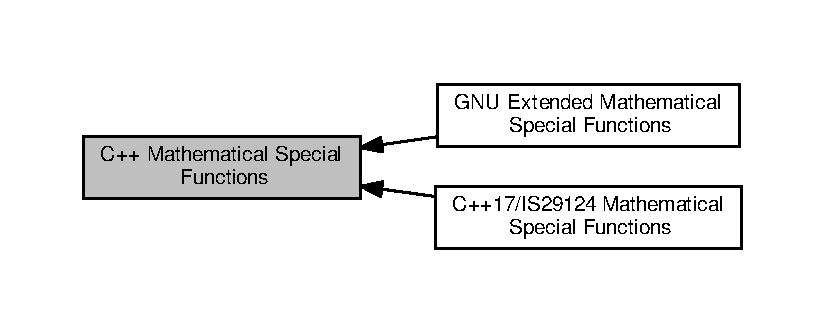
\includegraphics[width=350pt]{group__math__spec__func}
\end{center}
\end{figure}
\subsection*{Modules}
\begin{DoxyCompactItemize}
\item 
\hyperlink{group__cxx17__math__spec__func}{C++17/\+I\+S29124 Mathematical Special Functions}
\item 
\hyperlink{group__gnu__math__spec__func}{G\+N\+U Extended Mathematical Special Functions}
\end{DoxyCompactItemize}


\subsection{Detailed Description}
A collection of advanced mathematical special functions. 
\hypertarget{group__tr29124__math__spec__func}{}\section{C++17/\+I\+S29124 Mathematical Special Functions}
\label{group__tr29124__math__spec__func}\index{C++17/\+I\+S29124 Mathematical Special Functions@{C++17/\+I\+S29124 Mathematical Special Functions}}
Collaboration diagram for C++17/\+I\+S29124 Mathematical Special Functions\+:
\nopagebreak
\begin{figure}[H]
\begin{center}
\leavevmode
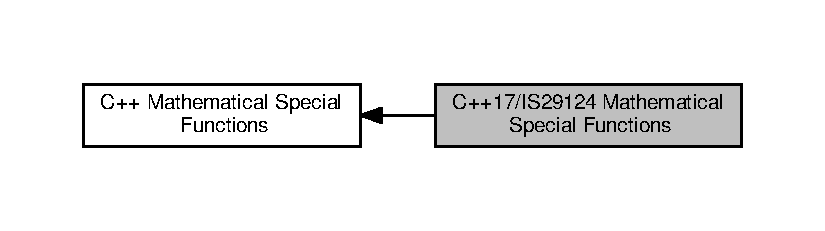
\includegraphics[width=350pt]{group__tr29124__math__spec__func}
\end{center}
\end{figure}
\subsection*{Functions}
\begin{DoxyCompactItemize}
\item 
{\footnotesize template$<$typename \+\_\+\+Tp $>$ }\\\+\_\+\+\_\+gnu\+\_\+cxx\+::\+\_\+\+\_\+promote$<$ \+\_\+\+Tp $>$\+::\+\_\+\+\_\+type \hyperlink{group__tr29124__math__spec__func_ga377bb7e038c464a27dfe0573fd2d7b33}{std\+::assoc\+\_\+laguerre} (unsigned int \+\_\+\+\_\+n, unsigned int \+\_\+\+\_\+m, \+\_\+\+Tp \+\_\+\+\_\+x)
\item 
float \hyperlink{group__tr29124__math__spec__func_gaf83d98f350a1cfcebee6a1f723cf90d2}{std\+::assoc\+\_\+laguerref} (unsigned int \+\_\+\+\_\+n, unsigned int \+\_\+\+\_\+m, float \+\_\+\+\_\+x)
\item 
long double \hyperlink{group__tr29124__math__spec__func_gac8e245671fb2df5de5fd978d03081f6c}{std\+::assoc\+\_\+laguerrel} (unsigned int \+\_\+\+\_\+n, unsigned int \+\_\+\+\_\+m, long double \+\_\+\+\_\+x)
\item 
{\footnotesize template$<$typename \+\_\+\+Tp $>$ }\\\+\_\+\+\_\+gnu\+\_\+cxx\+::\+\_\+\+\_\+promote$<$ \+\_\+\+Tp $>$\+::\+\_\+\+\_\+type \hyperlink{group__tr29124__math__spec__func_ga355349f79119c1fd1e2a9351cec57f0f}{std\+::assoc\+\_\+legendre} (unsigned int \+\_\+\+\_\+l, unsigned int \+\_\+\+\_\+m, \+\_\+\+Tp \+\_\+\+\_\+x)
\item 
float \hyperlink{group__tr29124__math__spec__func_ga3ced07ddd24bf4af56e2712d148e7f57}{std\+::assoc\+\_\+legendref} (unsigned int \+\_\+\+\_\+l, unsigned int \+\_\+\+\_\+m, float \+\_\+\+\_\+x)
\item 
long double \hyperlink{group__tr29124__math__spec__func_ga55977b425a539146f060dec1c8003344}{std\+::assoc\+\_\+legendrel} (unsigned int \+\_\+\+\_\+l, unsigned int \+\_\+\+\_\+m, long double \+\_\+\+\_\+x)
\item 
{\footnotesize template$<$typename \+\_\+\+Tpa , typename \+\_\+\+Tpb $>$ }\\\+\_\+\+\_\+gnu\+\_\+cxx\+::\+\_\+\+\_\+promote\+\_\+2$<$ \+\_\+\+Tpa, \+\_\+\+Tpb $>$\+::\+\_\+\+\_\+type \hyperlink{group__tr29124__math__spec__func_ga6a7220c87c942db48b18b527d92bbd2d}{std\+::beta} (\+\_\+\+Tpa \+\_\+\+\_\+a, \+\_\+\+Tpb \+\_\+\+\_\+b)
\item 
float \hyperlink{group__tr29124__math__spec__func_ga12dc61ee4c09172151cf092ed387e203}{std\+::betaf} (float \+\_\+\+\_\+a, float \+\_\+\+\_\+b)
\item 
long double \hyperlink{group__tr29124__math__spec__func_ga8caca1cef099f41a88111209c36ce06c}{std\+::betal} (long double \+\_\+\+\_\+a, long double \+\_\+\+\_\+b)
\item 
{\footnotesize template$<$typename \+\_\+\+Tp $>$ }\\\+\_\+\+\_\+gnu\+\_\+cxx\+::\+\_\+\+\_\+promote$<$ \+\_\+\+Tp $>$\+::\+\_\+\+\_\+type \hyperlink{group__tr29124__math__spec__func_gac559500c604c43ea943d593c9ad9d289}{std\+::comp\+\_\+ellint\+\_\+1} (\+\_\+\+Tp \+\_\+\+\_\+k)
\item 
float \hyperlink{group__tr29124__math__spec__func_ga7fb5be999a8125cf7e55e630eb8444a1}{std\+::comp\+\_\+ellint\+\_\+1f} (float \+\_\+\+\_\+k)
\item 
long double \hyperlink{group__tr29124__math__spec__func_ga7247d3dd77c1ff5df3c059fed862dc48}{std\+::comp\+\_\+ellint\+\_\+1l} (long double \+\_\+\+\_\+k)
\item 
{\footnotesize template$<$typename \+\_\+\+Tp $>$ }\\\+\_\+\+\_\+gnu\+\_\+cxx\+::\+\_\+\+\_\+promote$<$ \+\_\+\+Tp $>$\+::\+\_\+\+\_\+type \hyperlink{group__tr29124__math__spec__func_ga22fcc678829f0daf2de257896378e7e0}{std\+::comp\+\_\+ellint\+\_\+2} (\+\_\+\+Tp \+\_\+\+\_\+k)
\item 
float \hyperlink{group__tr29124__math__spec__func_ga21700f2f125c42b1f1da1f9c7eea1135}{std\+::comp\+\_\+ellint\+\_\+2f} (float \+\_\+\+\_\+k)
\item 
long double \hyperlink{group__tr29124__math__spec__func_ga47b647ec386c8d4b18a030c97842df18}{std\+::comp\+\_\+ellint\+\_\+2l} (long double \+\_\+\+\_\+k)
\item 
{\footnotesize template$<$typename \+\_\+\+Tp , typename \+\_\+\+Tpn $>$ }\\\+\_\+\+\_\+gnu\+\_\+cxx\+::\+\_\+\+\_\+promote\+\_\+2$<$ \+\_\+\+Tp, \+\_\+\+Tpn $>$\+::\+\_\+\+\_\+type \hyperlink{group__tr29124__math__spec__func_gad833404645e24b7f0598a640ff92d623}{std\+::comp\+\_\+ellint\+\_\+3} (\+\_\+\+Tp \+\_\+\+\_\+k, \+\_\+\+Tpn \+\_\+\+\_\+nu)
\item 
float \hyperlink{group__tr29124__math__spec__func_ga76834d3112f777703330892303267a39}{std\+::comp\+\_\+ellint\+\_\+3f} (float \+\_\+\+\_\+k, float \+\_\+\+\_\+nu)
\begin{DoxyCompactList}\small\item\em Return the complete elliptic integral of the third kind $ \Pi(k,\nu) $ for {\ttfamily float} modulus {\ttfamily k}. \end{DoxyCompactList}\item 
long double \hyperlink{group__tr29124__math__spec__func_ga1ca081fee102cd0d4d6b091285e495e5}{std\+::comp\+\_\+ellint\+\_\+3l} (long double \+\_\+\+\_\+k, long double \+\_\+\+\_\+nu)
\begin{DoxyCompactList}\small\item\em Return the complete elliptic integral of the third kind $ \Pi(k,\nu) $ for {\ttfamily long double} modulus {\ttfamily k}. \end{DoxyCompactList}\item 
{\footnotesize template$<$typename \+\_\+\+Tpnu , typename \+\_\+\+Tp $>$ }\\\+\_\+\+\_\+gnu\+\_\+cxx\+::\+\_\+\+\_\+promote\+\_\+2$<$ \+\_\+\+Tpnu, \+\_\+\+Tp $>$\+::\+\_\+\+\_\+type \hyperlink{group__tr29124__math__spec__func_ga1c9b5a5c36f000a4f0a55f7fcc486cb0}{std\+::cyl\+\_\+bessel\+\_\+i} (\+\_\+\+Tpnu \+\_\+\+\_\+nu, \+\_\+\+Tp \+\_\+\+\_\+x)
\item 
float \hyperlink{group__tr29124__math__spec__func_gaaf738427d4da0bda66bc2274dfb853a7}{std\+::cyl\+\_\+bessel\+\_\+if} (float \+\_\+\+\_\+nu, float \+\_\+\+\_\+x)
\item 
long double \hyperlink{group__tr29124__math__spec__func_gab7962629216d03efb8ecaa3f70c6878f}{std\+::cyl\+\_\+bessel\+\_\+il} (long double \+\_\+\+\_\+nu, long double \+\_\+\+\_\+x)
\item 
{\footnotesize template$<$typename \+\_\+\+Tpnu , typename \+\_\+\+Tp $>$ }\\\+\_\+\+\_\+gnu\+\_\+cxx\+::\+\_\+\+\_\+promote\+\_\+2$<$ \+\_\+\+Tpnu, \+\_\+\+Tp $>$\+::\+\_\+\+\_\+type \hyperlink{group__tr29124__math__spec__func_ga47e21a13b6d68d0d7f057699bd3b3ce0}{std\+::cyl\+\_\+bessel\+\_\+j} (\+\_\+\+Tpnu \+\_\+\+\_\+nu, \+\_\+\+Tp \+\_\+\+\_\+x)
\item 
float \hyperlink{group__tr29124__math__spec__func_ga15731a7bccd6351d28353e3c4c2a2d23}{std\+::cyl\+\_\+bessel\+\_\+jf} (float \+\_\+\+\_\+nu, float \+\_\+\+\_\+x)
\item 
long double \hyperlink{group__tr29124__math__spec__func_gade8e94a80520a8b628b2d658755b25c0}{std\+::cyl\+\_\+bessel\+\_\+jl} (long double \+\_\+\+\_\+nu, long double \+\_\+\+\_\+x)
\item 
{\footnotesize template$<$typename \+\_\+\+Tpnu , typename \+\_\+\+Tp $>$ }\\\+\_\+\+\_\+gnu\+\_\+cxx\+::\+\_\+\+\_\+promote\+\_\+2$<$ \+\_\+\+Tpnu, \+\_\+\+Tp $>$\+::\+\_\+\+\_\+type \hyperlink{group__tr29124__math__spec__func_ga76dcd3884620955680112aca0d327ada}{std\+::cyl\+\_\+bessel\+\_\+k} (\+\_\+\+Tpnu \+\_\+\+\_\+nu, \+\_\+\+Tp \+\_\+\+\_\+x)
\item 
float \hyperlink{group__tr29124__math__spec__func_ga1f50047f9aab0ec8b1a1615fe9fbe32f}{std\+::cyl\+\_\+bessel\+\_\+kf} (float \+\_\+\+\_\+nu, float \+\_\+\+\_\+x)
\item 
long double \hyperlink{group__tr29124__math__spec__func_gac35194b926270d7857d651e06198c7d3}{std\+::cyl\+\_\+bessel\+\_\+kl} (long double \+\_\+\+\_\+nu, long double \+\_\+\+\_\+x)
\item 
{\footnotesize template$<$typename \+\_\+\+Tpnu , typename \+\_\+\+Tp $>$ }\\\+\_\+\+\_\+gnu\+\_\+cxx\+::\+\_\+\+\_\+promote\+\_\+2$<$ \+\_\+\+Tpnu, \+\_\+\+Tp $>$\+::\+\_\+\+\_\+type \hyperlink{group__tr29124__math__spec__func_ga5b7c72ab85e361cbd73f1a3b5f0725a6}{std\+::cyl\+\_\+neumann} (\+\_\+\+Tpnu \+\_\+\+\_\+nu, \+\_\+\+Tp \+\_\+\+\_\+x)
\item 
float \hyperlink{group__tr29124__math__spec__func_ga604c13e8f2bb7cd3c7c91d8b19d6b13a}{std\+::cyl\+\_\+neumannf} (float \+\_\+\+\_\+nu, float \+\_\+\+\_\+x)
\item 
long double \hyperlink{group__tr29124__math__spec__func_gaf8986bae9a523c48d861d233835bda8f}{std\+::cyl\+\_\+neumannl} (long double \+\_\+\+\_\+nu, long double \+\_\+\+\_\+x)
\item 
{\footnotesize template$<$typename \+\_\+\+Tp , typename \+\_\+\+Tpp $>$ }\\\+\_\+\+\_\+gnu\+\_\+cxx\+::\+\_\+\+\_\+promote\+\_\+2$<$ \+\_\+\+Tp, \+\_\+\+Tpp $>$\+::\+\_\+\+\_\+type \hyperlink{group__tr29124__math__spec__func_gae6b3df5556f38a7d72f9b4457d856f9c}{std\+::ellint\+\_\+1} (\+\_\+\+Tp \+\_\+\+\_\+k, \+\_\+\+Tpp \+\_\+\+\_\+phi)
\item 
float \hyperlink{group__tr29124__math__spec__func_ga308d23d70f4b5e848eb7a4173628ef3b}{std\+::ellint\+\_\+1f} (float \+\_\+\+\_\+k, float \+\_\+\+\_\+phi)
\item 
long double \hyperlink{group__tr29124__math__spec__func_ga795383fa51e02351000b410b478d824f}{std\+::ellint\+\_\+1l} (long double \+\_\+\+\_\+k, long double \+\_\+\+\_\+phi)
\item 
{\footnotesize template$<$typename \+\_\+\+Tp , typename \+\_\+\+Tpp $>$ }\\\+\_\+\+\_\+gnu\+\_\+cxx\+::\+\_\+\+\_\+promote\+\_\+2$<$ \+\_\+\+Tp, \+\_\+\+Tpp $>$\+::\+\_\+\+\_\+type \hyperlink{group__tr29124__math__spec__func_gad6dd71db2b3f90d24ff49bf8cf37bc37}{std\+::ellint\+\_\+2} (\+\_\+\+Tp \+\_\+\+\_\+k, \+\_\+\+Tpp \+\_\+\+\_\+phi)
\item 
float \hyperlink{group__tr29124__math__spec__func_ga594a730163c6228c75b152462700062b}{std\+::ellint\+\_\+2f} (float \+\_\+\+\_\+k, float \+\_\+\+\_\+phi)
\begin{DoxyCompactList}\small\item\em Return the incomplete elliptic integral of the second kind $ E(k,\phi) $ for {\ttfamily float} argument. \end{DoxyCompactList}\item 
long double \hyperlink{group__tr29124__math__spec__func_ga5c791332d374a809d8ca16c69a1a30f5}{std\+::ellint\+\_\+2l} (long double \+\_\+\+\_\+k, long double \+\_\+\+\_\+phi)
\begin{DoxyCompactList}\small\item\em Return the incomplete elliptic integral of the second kind $ E(k,\phi) $. \end{DoxyCompactList}\item 
{\footnotesize template$<$typename \+\_\+\+Tp , typename \+\_\+\+Tpn , typename \+\_\+\+Tpp $>$ }\\\+\_\+\+\_\+gnu\+\_\+cxx\+::\+\_\+\+\_\+promote\+\_\+3$<$ \+\_\+\+Tp, \+\_\+\+Tpn, \+\_\+\+Tpp $>$\+::\+\_\+\+\_\+type \hyperlink{group__tr29124__math__spec__func_ga20832e3a67d25cc3d415cafc88019ac3}{std\+::ellint\+\_\+3} (\+\_\+\+Tp \+\_\+\+\_\+k, \+\_\+\+Tpn \+\_\+\+\_\+nu, \+\_\+\+Tpp \+\_\+\+\_\+phi)
\begin{DoxyCompactList}\small\item\em Return the incomplete elliptic integral of the third kind $ \Pi(k,\nu,\phi) $. \end{DoxyCompactList}\item 
float \hyperlink{group__tr29124__math__spec__func_ga1a80bd2c15bc9fbecda2630a9e9409e7}{std\+::ellint\+\_\+3f} (float \+\_\+\+\_\+k, float \+\_\+\+\_\+nu, float \+\_\+\+\_\+phi)
\begin{DoxyCompactList}\small\item\em Return the incomplete elliptic integral of the third kind $ \Pi(k,\nu,\phi) $ for {\ttfamily float} argument. \end{DoxyCompactList}\item 
long double \hyperlink{group__tr29124__math__spec__func_gaa8c0e5864df8769021a7f3e21a30c5d2}{std\+::ellint\+\_\+3l} (long double \+\_\+\+\_\+k, long double \+\_\+\+\_\+nu, long double \+\_\+\+\_\+phi)
\begin{DoxyCompactList}\small\item\em Return the incomplete elliptic integral of the third kind $ \Pi(k,\nu,\phi) $. \end{DoxyCompactList}\item 
{\footnotesize template$<$typename \+\_\+\+Tp $>$ }\\\+\_\+\+\_\+gnu\+\_\+cxx\+::\+\_\+\+\_\+promote$<$ \+\_\+\+Tp $>$\+::\+\_\+\+\_\+type \hyperlink{group__tr29124__math__spec__func_ga88ba17f5d050a6973ca4db1bf6e90590}{std\+::expint} (\+\_\+\+Tp \+\_\+\+\_\+x)
\item 
float \hyperlink{group__tr29124__math__spec__func_ga5842816f6eed2594e0a327df4e4a2a47}{std\+::expintf} (float \+\_\+\+\_\+x)
\item 
long double \hyperlink{group__tr29124__math__spec__func_ga1329130b32328d0666e290ee5931fa4f}{std\+::expintl} (long double \+\_\+\+\_\+x)
\item 
{\footnotesize template$<$typename \+\_\+\+Tp $>$ }\\\+\_\+\+\_\+gnu\+\_\+cxx\+::\+\_\+\+\_\+promote$<$ \+\_\+\+Tp $>$\+::\+\_\+\+\_\+type \hyperlink{group__tr29124__math__spec__func_ga97632b8bf77c323b2369e8d327965bdf}{std\+::hermite} (unsigned int \+\_\+\+\_\+n, \+\_\+\+Tp \+\_\+\+\_\+x)
\item 
float \hyperlink{group__tr29124__math__spec__func_ga94dae7444bb349e33057a92932db8abe}{std\+::hermitef} (unsigned int \+\_\+\+\_\+n, float \+\_\+\+\_\+x)
\item 
long double \hyperlink{group__tr29124__math__spec__func_ga21f8e312ee3e65286f86bf141b0f32e0}{std\+::hermitel} (unsigned int \+\_\+\+\_\+n, long double \+\_\+\+\_\+x)
\item 
{\footnotesize template$<$typename \+\_\+\+Tp $>$ }\\\+\_\+\+\_\+gnu\+\_\+cxx\+::\+\_\+\+\_\+promote$<$ \+\_\+\+Tp $>$\+::\+\_\+\+\_\+type \hyperlink{group__tr29124__math__spec__func_gacae65579b397fddcd27954380d364a58}{std\+::laguerre} (unsigned int \+\_\+\+\_\+n, \+\_\+\+Tp \+\_\+\+\_\+x)
\item 
float \hyperlink{group__tr29124__math__spec__func_gada763419b0e21b38e38daa8b6eb56a8c}{std\+::laguerref} (unsigned int \+\_\+\+\_\+n, float \+\_\+\+\_\+x)
\item 
long double \hyperlink{group__tr29124__math__spec__func_gaaf8b141edf9163b37ea4f2ed3e0191fc}{std\+::laguerrel} (unsigned int \+\_\+\+\_\+n, long double \+\_\+\+\_\+x)
\item 
{\footnotesize template$<$typename \+\_\+\+Tp $>$ }\\\+\_\+\+\_\+gnu\+\_\+cxx\+::\+\_\+\+\_\+promote$<$ \+\_\+\+Tp $>$\+::\+\_\+\+\_\+type \hyperlink{group__tr29124__math__spec__func_gaf6eac7fcb98e25b8f3f7d1b95fa7add8}{std\+::legendre} (unsigned int \+\_\+\+\_\+l, \+\_\+\+Tp \+\_\+\+\_\+x)
\item 
float \hyperlink{group__tr29124__math__spec__func_gaed94e3c664c99f5204da75be75aeac21}{std\+::legendref} (unsigned int \+\_\+\+\_\+l, float \+\_\+\+\_\+x)
\item 
long double \hyperlink{group__tr29124__math__spec__func_ga1b39bc22e3cc4860d08eb54099460391}{std\+::legendrel} (unsigned int \+\_\+\+\_\+l, long double \+\_\+\+\_\+x)
\item 
{\footnotesize template$<$typename \+\_\+\+Tp $>$ }\\\+\_\+\+\_\+gnu\+\_\+cxx\+::\+\_\+\+\_\+promote$<$ \+\_\+\+Tp $>$\+::\+\_\+\+\_\+type \hyperlink{group__tr29124__math__spec__func_ga67a6bfed9b6ab692e8c798b674431424}{std\+::riemann\+\_\+zeta} (\+\_\+\+Tp \+\_\+\+\_\+s)
\item 
float \hyperlink{group__tr29124__math__spec__func_gaf92063315061a56d3e2c4053156d968e}{std\+::riemann\+\_\+zetaf} (float \+\_\+\+\_\+s)
\item 
long double \hyperlink{group__tr29124__math__spec__func_ga1e92da3b878d75270f38d3ec9b513086}{std\+::riemann\+\_\+zetal} (long double \+\_\+\+\_\+s)
\item 
{\footnotesize template$<$typename \+\_\+\+Tp $>$ }\\\+\_\+\+\_\+gnu\+\_\+cxx\+::\+\_\+\+\_\+promote$<$ \+\_\+\+Tp $>$\+::\+\_\+\+\_\+type \hyperlink{group__tr29124__math__spec__func_ga478e517ed975bcb256de230e64f0fda5}{std\+::sph\+\_\+bessel} (unsigned int \+\_\+\+\_\+n, \+\_\+\+Tp \+\_\+\+\_\+x)
\item 
float \hyperlink{group__tr29124__math__spec__func_ga534e36e1dcefad8daec98920db16eec4}{std\+::sph\+\_\+besself} (unsigned int \+\_\+\+\_\+n, float \+\_\+\+\_\+x)
\item 
long double \hyperlink{group__tr29124__math__spec__func_ga11d72b1af81ce9da3c878a25087ee927}{std\+::sph\+\_\+bessell} (unsigned int \+\_\+\+\_\+n, long double \+\_\+\+\_\+x)
\item 
{\footnotesize template$<$typename \+\_\+\+Tp $>$ }\\\+\_\+\+\_\+gnu\+\_\+cxx\+::\+\_\+\+\_\+promote$<$ \+\_\+\+Tp $>$\+::\+\_\+\+\_\+type \hyperlink{group__tr29124__math__spec__func_ga573842c12247b87746b548f1945755a8}{std\+::sph\+\_\+legendre} (unsigned int \+\_\+\+\_\+l, unsigned int \+\_\+\+\_\+m, \+\_\+\+Tp \+\_\+\+\_\+theta)
\item 
float \hyperlink{group__tr29124__math__spec__func_gaae635d28c06a3be2679901b382090852}{std\+::sph\+\_\+legendref} (unsigned int \+\_\+\+\_\+l, unsigned int \+\_\+\+\_\+m, float \+\_\+\+\_\+theta)
\item 
long double \hyperlink{group__tr29124__math__spec__func_ga2f6618dea1847f09fd67f3c974c1910d}{std\+::sph\+\_\+legendrel} (unsigned int \+\_\+\+\_\+l, unsigned int \+\_\+\+\_\+m, long double \+\_\+\+\_\+theta)
\item 
{\footnotesize template$<$typename \+\_\+\+Tp $>$ }\\\+\_\+\+\_\+gnu\+\_\+cxx\+::\+\_\+\+\_\+promote$<$ \+\_\+\+Tp $>$\+::\+\_\+\+\_\+type \hyperlink{group__tr29124__math__spec__func_ga1cf4362a67ab5bae9e6b69c867e85371}{std\+::sph\+\_\+neumann} (unsigned int \+\_\+\+\_\+n, \+\_\+\+Tp \+\_\+\+\_\+x)
\item 
float \hyperlink{group__tr29124__math__spec__func_ga789143122fa99536329bc2d1b1aac2f0}{std\+::sph\+\_\+neumannf} (unsigned int \+\_\+\+\_\+n, float \+\_\+\+\_\+x)
\item 
long double \hyperlink{group__tr29124__math__spec__func_ga3cededa9b6e4601f190c3811e6aabfd6}{std\+::sph\+\_\+neumannl} (unsigned int \+\_\+\+\_\+n, long double \+\_\+\+\_\+x)
\end{DoxyCompactItemize}


\subsection{Detailed Description}
A collection of advanced mathematical special functions for C++17 and I\+S29124. 

\subsection{Function Documentation}
\hypertarget{group__tr29124__math__spec__func_ga377bb7e038c464a27dfe0573fd2d7b33}{}\index{C++17/\+I\+S29124 Mathematical Special Functions@{C++17/\+I\+S29124 Mathematical Special Functions}!assoc\+\_\+laguerre@{assoc\+\_\+laguerre}}
\index{assoc\+\_\+laguerre@{assoc\+\_\+laguerre}!C++17/\+I\+S29124 Mathematical Special Functions@{C++17/\+I\+S29124 Mathematical Special Functions}}
\subsubsection[{assoc\+\_\+laguerre}]{\setlength{\rightskip}{0pt plus 5cm}template$<$typename \+\_\+\+Tp $>$ \+\_\+\+\_\+gnu\+\_\+cxx\+::\+\_\+\+\_\+promote$<$\+\_\+\+Tp$>$\+::\+\_\+\+\_\+type std\+::assoc\+\_\+laguerre (
\begin{DoxyParamCaption}
\item[{unsigned int}]{\+\_\+\+\_\+n, }
\item[{unsigned int}]{\+\_\+\+\_\+m, }
\item[{\+\_\+\+Tp}]{\+\_\+\+\_\+x}
\end{DoxyParamCaption}
)\hspace{0.3cm}{\ttfamily [inline]}}\label{group__tr29124__math__spec__func_ga377bb7e038c464a27dfe0573fd2d7b33}
Return the associated Laguerre polynomial of nonnegative order {\ttfamily n}, nonnegative degree {\ttfamily m} and real argument {\ttfamily x\+:} $ L_n^m(x) $.

The associated Laguerre function of real degree $ \alpha $, $ L_n^\alpha(x) $, is defined by \[ L_n^\alpha(x) = \frac{(\alpha + 1)_n}{n!} {}_1F_1(-n; \alpha + 1; x) \] where $ (\alpha)_n $ is the Pochhammer symbol and $ {}_1F_1(a; c; x) $ is the confluent hypergeometric function.

The associated Laguerre polynomial is defined for integral degree $ \alpha = m $ by\+: \[ L_n^m(x) = (-1)^m \frac{d^m}{dx^m} L_{n + m}(x) \] where the Laguerre polynomial is defined by\+: \[ L_n(x) = \frac{e^x}{n!} \frac{d^n}{dx^n} (x^ne^{-x}) \] and $ x >= 0 $. \begin{DoxySeeAlso}{See also}
\hyperlink{group__tr29124__math__spec__func_gacae65579b397fddcd27954380d364a58}{laguerre} for details of the Laguerre function of degree {\ttfamily n} 
\end{DoxySeeAlso}

\begin{DoxyTemplParams}{Template Parameters}
{\em \+\_\+\+Tp} & The floating-\/point type of the argument {\ttfamily \+\_\+\+\_\+x}. \\
\hline
\end{DoxyTemplParams}

\begin{DoxyParams}{Parameters}
{\em \+\_\+\+\_\+n} & The order of the Laguerre function, {\ttfamily \+\_\+\+\_\+n $>$= 0}. \\
\hline
{\em \+\_\+\+\_\+m} & The degree of the Laguerre function, {\ttfamily \+\_\+\+\_\+m $>$= 0}. \\
\hline
{\em \+\_\+\+\_\+x} & The argument of the Laguerre function, {\ttfamily \+\_\+\+\_\+x $>$= 0}. \\
\hline
\end{DoxyParams}

\begin{DoxyExceptions}{Exceptions}
{\em std\+::domain\+\_\+error} & if {\ttfamily \+\_\+\+\_\+x $<$ 0}. \\
\hline
\end{DoxyExceptions}


Definition at line 299 of file specfun.\+h.

\hypertarget{group__tr29124__math__spec__func_gaf83d98f350a1cfcebee6a1f723cf90d2}{}\index{C++17/\+I\+S29124 Mathematical Special Functions@{C++17/\+I\+S29124 Mathematical Special Functions}!assoc\+\_\+laguerref@{assoc\+\_\+laguerref}}
\index{assoc\+\_\+laguerref@{assoc\+\_\+laguerref}!C++17/\+I\+S29124 Mathematical Special Functions@{C++17/\+I\+S29124 Mathematical Special Functions}}
\subsubsection[{assoc\+\_\+laguerref}]{\setlength{\rightskip}{0pt plus 5cm}float std\+::assoc\+\_\+laguerref (
\begin{DoxyParamCaption}
\item[{unsigned int}]{\+\_\+\+\_\+n, }
\item[{unsigned int}]{\+\_\+\+\_\+m, }
\item[{float}]{\+\_\+\+\_\+x}
\end{DoxyParamCaption}
)\hspace{0.3cm}{\ttfamily [inline]}}\label{group__tr29124__math__spec__func_gaf83d98f350a1cfcebee6a1f723cf90d2}
Return the associated Laguerre polynomial of order {\ttfamily n}, degree {\ttfamily m\+:} $ L_n^m(x) $ for {\ttfamily float} argument.

\begin{DoxySeeAlso}{See also}
\hyperlink{group__tr29124__math__spec__func_ga377bb7e038c464a27dfe0573fd2d7b33}{assoc\+\_\+laguerre} for more details. 
\end{DoxySeeAlso}


Definition at line 253 of file specfun.\+h.

\hypertarget{group__tr29124__math__spec__func_gac8e245671fb2df5de5fd978d03081f6c}{}\index{C++17/\+I\+S29124 Mathematical Special Functions@{C++17/\+I\+S29124 Mathematical Special Functions}!assoc\+\_\+laguerrel@{assoc\+\_\+laguerrel}}
\index{assoc\+\_\+laguerrel@{assoc\+\_\+laguerrel}!C++17/\+I\+S29124 Mathematical Special Functions@{C++17/\+I\+S29124 Mathematical Special Functions}}
\subsubsection[{assoc\+\_\+laguerrel}]{\setlength{\rightskip}{0pt plus 5cm}long double std\+::assoc\+\_\+laguerrel (
\begin{DoxyParamCaption}
\item[{unsigned int}]{\+\_\+\+\_\+n, }
\item[{unsigned int}]{\+\_\+\+\_\+m, }
\item[{long double}]{\+\_\+\+\_\+x}
\end{DoxyParamCaption}
)\hspace{0.3cm}{\ttfamily [inline]}}\label{group__tr29124__math__spec__func_gac8e245671fb2df5de5fd978d03081f6c}
Return the associated Laguerre polynomial of order {\ttfamily n}, degree {\ttfamily m\+:} $ L_n^m(x) $.

\begin{DoxySeeAlso}{See also}
\hyperlink{group__tr29124__math__spec__func_ga377bb7e038c464a27dfe0573fd2d7b33}{assoc\+\_\+laguerre} for more details. 
\end{DoxySeeAlso}


Definition at line 263 of file specfun.\+h.

\hypertarget{group__tr29124__math__spec__func_ga355349f79119c1fd1e2a9351cec57f0f}{}\index{C++17/\+I\+S29124 Mathematical Special Functions@{C++17/\+I\+S29124 Mathematical Special Functions}!assoc\+\_\+legendre@{assoc\+\_\+legendre}}
\index{assoc\+\_\+legendre@{assoc\+\_\+legendre}!C++17/\+I\+S29124 Mathematical Special Functions@{C++17/\+I\+S29124 Mathematical Special Functions}}
\subsubsection[{assoc\+\_\+legendre}]{\setlength{\rightskip}{0pt plus 5cm}template$<$typename \+\_\+\+Tp $>$ \+\_\+\+\_\+gnu\+\_\+cxx\+::\+\_\+\+\_\+promote$<$\+\_\+\+Tp$>$\+::\+\_\+\+\_\+type std\+::assoc\+\_\+legendre (
\begin{DoxyParamCaption}
\item[{unsigned int}]{\+\_\+\+\_\+l, }
\item[{unsigned int}]{\+\_\+\+\_\+m, }
\item[{\+\_\+\+Tp}]{\+\_\+\+\_\+x}
\end{DoxyParamCaption}
)\hspace{0.3cm}{\ttfamily [inline]}}\label{group__tr29124__math__spec__func_ga355349f79119c1fd1e2a9351cec57f0f}
Return the associated Legendre function of degree {\ttfamily l} and order {\ttfamily m}.

The associated Legendre function is derived from the Legendre function $ P_l(x) $ by the Rodrigues formula\+: \[ P_l^m(x) = (1 - x^2)^{m/2}\frac{d^m}{dx^m}P_l(x) \] \begin{DoxySeeAlso}{See also}
\hyperlink{group__tr29124__math__spec__func_gaf6eac7fcb98e25b8f3f7d1b95fa7add8}{legendre} for details of the Legendre function of degree {\ttfamily l} 
\end{DoxySeeAlso}

\begin{DoxyTemplParams}{Template Parameters}
{\em \+\_\+\+Tp} & The floating-\/point type of the argument {\ttfamily \+\_\+\+\_\+x}. \\
\hline
\end{DoxyTemplParams}

\begin{DoxyParams}{Parameters}
{\em \+\_\+\+\_\+l} & The degree {\ttfamily \+\_\+\+\_\+l $>$= 0}. \\
\hline
{\em \+\_\+\+\_\+m} & The order {\ttfamily \+\_\+\+\_\+m $<$= l}. \\
\hline
{\em \+\_\+\+\_\+x} & The argument, {\ttfamily abs(\+\_\+\+\_\+x) $<$= 1}. \\
\hline
\end{DoxyParams}

\begin{DoxyExceptions}{Exceptions}
{\em std\+::domain\+\_\+error} & if {\ttfamily abs(\+\_\+\+\_\+x) $>$ 1}. \\
\hline
\end{DoxyExceptions}


Definition at line 344 of file specfun.\+h.

\hypertarget{group__tr29124__math__spec__func_ga3ced07ddd24bf4af56e2712d148e7f57}{}\index{C++17/\+I\+S29124 Mathematical Special Functions@{C++17/\+I\+S29124 Mathematical Special Functions}!assoc\+\_\+legendref@{assoc\+\_\+legendref}}
\index{assoc\+\_\+legendref@{assoc\+\_\+legendref}!C++17/\+I\+S29124 Mathematical Special Functions@{C++17/\+I\+S29124 Mathematical Special Functions}}
\subsubsection[{assoc\+\_\+legendref}]{\setlength{\rightskip}{0pt plus 5cm}float std\+::assoc\+\_\+legendref (
\begin{DoxyParamCaption}
\item[{unsigned int}]{\+\_\+\+\_\+l, }
\item[{unsigned int}]{\+\_\+\+\_\+m, }
\item[{float}]{\+\_\+\+\_\+x}
\end{DoxyParamCaption}
)\hspace{0.3cm}{\ttfamily [inline]}}\label{group__tr29124__math__spec__func_ga3ced07ddd24bf4af56e2712d148e7f57}
Return the associated Legendre function of degree {\ttfamily l} and order {\ttfamily m} for {\ttfamily float} argument.

\begin{DoxySeeAlso}{See also}
\hyperlink{group__tr29124__math__spec__func_ga355349f79119c1fd1e2a9351cec57f0f}{assoc\+\_\+legendre} for more details. 
\end{DoxySeeAlso}


Definition at line 314 of file specfun.\+h.

\hypertarget{group__tr29124__math__spec__func_ga55977b425a539146f060dec1c8003344}{}\index{C++17/\+I\+S29124 Mathematical Special Functions@{C++17/\+I\+S29124 Mathematical Special Functions}!assoc\+\_\+legendrel@{assoc\+\_\+legendrel}}
\index{assoc\+\_\+legendrel@{assoc\+\_\+legendrel}!C++17/\+I\+S29124 Mathematical Special Functions@{C++17/\+I\+S29124 Mathematical Special Functions}}
\subsubsection[{assoc\+\_\+legendrel}]{\setlength{\rightskip}{0pt plus 5cm}long double std\+::assoc\+\_\+legendrel (
\begin{DoxyParamCaption}
\item[{unsigned int}]{\+\_\+\+\_\+l, }
\item[{unsigned int}]{\+\_\+\+\_\+m, }
\item[{long double}]{\+\_\+\+\_\+x}
\end{DoxyParamCaption}
)\hspace{0.3cm}{\ttfamily [inline]}}\label{group__tr29124__math__spec__func_ga55977b425a539146f060dec1c8003344}
Return the associated Legendre function of degree {\ttfamily l} and order {\ttfamily m}.

\begin{DoxySeeAlso}{See also}
\hyperlink{group__tr29124__math__spec__func_ga355349f79119c1fd1e2a9351cec57f0f}{assoc\+\_\+legendre} for more details. 
\end{DoxySeeAlso}


Definition at line 323 of file specfun.\+h.

\hypertarget{group__tr29124__math__spec__func_ga6a7220c87c942db48b18b527d92bbd2d}{}\index{C++17/\+I\+S29124 Mathematical Special Functions@{C++17/\+I\+S29124 Mathematical Special Functions}!beta@{beta}}
\index{beta@{beta}!C++17/\+I\+S29124 Mathematical Special Functions@{C++17/\+I\+S29124 Mathematical Special Functions}}
\subsubsection[{beta}]{\setlength{\rightskip}{0pt plus 5cm}template$<$typename \+\_\+\+Tpa , typename \+\_\+\+Tpb $>$ \+\_\+\+\_\+gnu\+\_\+cxx\+::\+\_\+\+\_\+promote\+\_\+2$<$\+\_\+\+Tpa, \+\_\+\+Tpb$>$\+::\+\_\+\+\_\+type std\+::beta (
\begin{DoxyParamCaption}
\item[{\+\_\+\+Tpa}]{\+\_\+\+\_\+a, }
\item[{\+\_\+\+Tpb}]{\+\_\+\+\_\+b}
\end{DoxyParamCaption}
)\hspace{0.3cm}{\ttfamily [inline]}}\label{group__tr29124__math__spec__func_ga6a7220c87c942db48b18b527d92bbd2d}
Return the beta function, $B(a,b)$, for real parameters {\ttfamily a}, {\ttfamily b}.

The beta function is defined by \[ B(a,b) = \int_0^1 t^{a - 1} (1 - t)^{b - 1} dt = \frac{\Gamma(a)\Gamma(b)}{\Gamma(a+b)} \] where $ x > 0 $ and $ y > 0 $


\begin{DoxyTemplParams}{Template Parameters}
{\em \+\_\+\+Tpa} & The floating-\/point type of the parameter {\ttfamily \+\_\+\+\_\+a}. \\
\hline
{\em \+\_\+\+Tpb} & The floating-\/point type of the parameter {\ttfamily \+\_\+\+\_\+b}. \\
\hline
\end{DoxyTemplParams}

\begin{DoxyParams}{Parameters}
{\em \+\_\+\+\_\+a} & The first argument of the beta function, {\ttfamily  \+\_\+\+\_\+a $>$ 0 }. \\
\hline
{\em \+\_\+\+\_\+b} & The second argument of the beta function, {\ttfamily  \+\_\+\+\_\+b $>$ 0 }. \\
\hline
\end{DoxyParams}

\begin{DoxyExceptions}{Exceptions}
{\em std\+::domain\+\_\+error} & if {\ttfamily  \+\_\+\+\_\+a $<$ 0 } or {\ttfamily  \+\_\+\+\_\+b $<$ 0 }. \\
\hline
\end{DoxyExceptions}


Definition at line 389 of file specfun.\+h.

\hypertarget{group__tr29124__math__spec__func_ga12dc61ee4c09172151cf092ed387e203}{}\index{C++17/\+I\+S29124 Mathematical Special Functions@{C++17/\+I\+S29124 Mathematical Special Functions}!betaf@{betaf}}
\index{betaf@{betaf}!C++17/\+I\+S29124 Mathematical Special Functions@{C++17/\+I\+S29124 Mathematical Special Functions}}
\subsubsection[{betaf}]{\setlength{\rightskip}{0pt plus 5cm}float std\+::betaf (
\begin{DoxyParamCaption}
\item[{float}]{\+\_\+\+\_\+a, }
\item[{float}]{\+\_\+\+\_\+b}
\end{DoxyParamCaption}
)\hspace{0.3cm}{\ttfamily [inline]}}\label{group__tr29124__math__spec__func_ga12dc61ee4c09172151cf092ed387e203}
Return the beta function, $ B(a,b) $, for {\ttfamily float} parameters {\ttfamily a}, {\ttfamily b}.

\begin{DoxySeeAlso}{See also}
\hyperlink{group__tr29124__math__spec__func_ga6a7220c87c942db48b18b527d92bbd2d}{beta} for more details. 
\end{DoxySeeAlso}


Definition at line 358 of file specfun.\+h.

\hypertarget{group__tr29124__math__spec__func_ga8caca1cef099f41a88111209c36ce06c}{}\index{C++17/\+I\+S29124 Mathematical Special Functions@{C++17/\+I\+S29124 Mathematical Special Functions}!betal@{betal}}
\index{betal@{betal}!C++17/\+I\+S29124 Mathematical Special Functions@{C++17/\+I\+S29124 Mathematical Special Functions}}
\subsubsection[{betal}]{\setlength{\rightskip}{0pt plus 5cm}long double std\+::betal (
\begin{DoxyParamCaption}
\item[{long double}]{\+\_\+\+\_\+a, }
\item[{long double}]{\+\_\+\+\_\+b}
\end{DoxyParamCaption}
)\hspace{0.3cm}{\ttfamily [inline]}}\label{group__tr29124__math__spec__func_ga8caca1cef099f41a88111209c36ce06c}
Return the beta function, $B(a,b)$, for long double parameters {\ttfamily a}, {\ttfamily b}.

\begin{DoxySeeAlso}{See also}
\hyperlink{group__tr29124__math__spec__func_ga6a7220c87c942db48b18b527d92bbd2d}{beta} for more details. 
\end{DoxySeeAlso}


Definition at line 368 of file specfun.\+h.

\hypertarget{group__tr29124__math__spec__func_gac559500c604c43ea943d593c9ad9d289}{}\index{C++17/\+I\+S29124 Mathematical Special Functions@{C++17/\+I\+S29124 Mathematical Special Functions}!comp\+\_\+ellint\+\_\+1@{comp\+\_\+ellint\+\_\+1}}
\index{comp\+\_\+ellint\+\_\+1@{comp\+\_\+ellint\+\_\+1}!C++17/\+I\+S29124 Mathematical Special Functions@{C++17/\+I\+S29124 Mathematical Special Functions}}
\subsubsection[{comp\+\_\+ellint\+\_\+1}]{\setlength{\rightskip}{0pt plus 5cm}template$<$typename \+\_\+\+Tp $>$ \+\_\+\+\_\+gnu\+\_\+cxx\+::\+\_\+\+\_\+promote$<$\+\_\+\+Tp$>$\+::\+\_\+\+\_\+type std\+::comp\+\_\+ellint\+\_\+1 (
\begin{DoxyParamCaption}
\item[{\+\_\+\+Tp}]{\+\_\+\+\_\+k}
\end{DoxyParamCaption}
)\hspace{0.3cm}{\ttfamily [inline]}}\label{group__tr29124__math__spec__func_gac559500c604c43ea943d593c9ad9d289}
Return the complete elliptic integral of the first kind $ K(k) $ for real modulus {\ttfamily k}.

The complete elliptic integral of the first kind is defined as \[ K(k) = F(k,\pi/2) = \int_0^{\pi/2}\frac{d\theta} {\sqrt{1 - k^2 sin^2\theta}} \] where $ F(k,\phi) $ is the incomplete elliptic integral of the first kind and the modulus $ |k| <= 1 $. \begin{DoxySeeAlso}{See also}
\hyperlink{group__tr29124__math__spec__func_gae6b3df5556f38a7d72f9b4457d856f9c}{ellint\+\_\+1} for details of the incomplete elliptic function of the first kind.
\end{DoxySeeAlso}

\begin{DoxyTemplParams}{Template Parameters}
{\em \+\_\+\+Tp} & The floating-\/point type of the modulus {\ttfamily \+\_\+\+\_\+k}. \\
\hline
\end{DoxyTemplParams}

\begin{DoxyParams}{Parameters}
{\em \+\_\+\+\_\+k} & The modulus, {\ttfamily  abs(\+\_\+\+\_\+k) $<$= 1 } \\
\hline
\end{DoxyParams}

\begin{DoxyExceptions}{Exceptions}
{\em std\+::domain\+\_\+error} & if {\ttfamily  abs(\+\_\+\+\_\+k) $>$ 1 }. \\
\hline
\end{DoxyExceptions}


Definition at line 437 of file specfun.\+h.

\hypertarget{group__tr29124__math__spec__func_ga7fb5be999a8125cf7e55e630eb8444a1}{}\index{C++17/\+I\+S29124 Mathematical Special Functions@{C++17/\+I\+S29124 Mathematical Special Functions}!comp\+\_\+ellint\+\_\+1f@{comp\+\_\+ellint\+\_\+1f}}
\index{comp\+\_\+ellint\+\_\+1f@{comp\+\_\+ellint\+\_\+1f}!C++17/\+I\+S29124 Mathematical Special Functions@{C++17/\+I\+S29124 Mathematical Special Functions}}
\subsubsection[{comp\+\_\+ellint\+\_\+1f}]{\setlength{\rightskip}{0pt plus 5cm}float std\+::comp\+\_\+ellint\+\_\+1f (
\begin{DoxyParamCaption}
\item[{float}]{\+\_\+\+\_\+k}
\end{DoxyParamCaption}
)\hspace{0.3cm}{\ttfamily [inline]}}\label{group__tr29124__math__spec__func_ga7fb5be999a8125cf7e55e630eb8444a1}
Return the complete elliptic integral of the first kind $ E(k) $ for {\ttfamily float} modulus {\ttfamily k}.

\begin{DoxySeeAlso}{See also}
\hyperlink{group__tr29124__math__spec__func_gac559500c604c43ea943d593c9ad9d289}{comp\+\_\+ellint\+\_\+1} for details. 
\end{DoxySeeAlso}


Definition at line 404 of file specfun.\+h.

\hypertarget{group__tr29124__math__spec__func_ga7247d3dd77c1ff5df3c059fed862dc48}{}\index{C++17/\+I\+S29124 Mathematical Special Functions@{C++17/\+I\+S29124 Mathematical Special Functions}!comp\+\_\+ellint\+\_\+1l@{comp\+\_\+ellint\+\_\+1l}}
\index{comp\+\_\+ellint\+\_\+1l@{comp\+\_\+ellint\+\_\+1l}!C++17/\+I\+S29124 Mathematical Special Functions@{C++17/\+I\+S29124 Mathematical Special Functions}}
\subsubsection[{comp\+\_\+ellint\+\_\+1l}]{\setlength{\rightskip}{0pt plus 5cm}long double std\+::comp\+\_\+ellint\+\_\+1l (
\begin{DoxyParamCaption}
\item[{long double}]{\+\_\+\+\_\+k}
\end{DoxyParamCaption}
)\hspace{0.3cm}{\ttfamily [inline]}}\label{group__tr29124__math__spec__func_ga7247d3dd77c1ff5df3c059fed862dc48}
Return the complete elliptic integral of the first kind $ E(k) $ for long double modulus {\ttfamily k}.

\begin{DoxySeeAlso}{See also}
\hyperlink{group__tr29124__math__spec__func_gac559500c604c43ea943d593c9ad9d289}{comp\+\_\+ellint\+\_\+1} for details. 
\end{DoxySeeAlso}


Definition at line 414 of file specfun.\+h.

\hypertarget{group__tr29124__math__spec__func_ga22fcc678829f0daf2de257896378e7e0}{}\index{C++17/\+I\+S29124 Mathematical Special Functions@{C++17/\+I\+S29124 Mathematical Special Functions}!comp\+\_\+ellint\+\_\+2@{comp\+\_\+ellint\+\_\+2}}
\index{comp\+\_\+ellint\+\_\+2@{comp\+\_\+ellint\+\_\+2}!C++17/\+I\+S29124 Mathematical Special Functions@{C++17/\+I\+S29124 Mathematical Special Functions}}
\subsubsection[{comp\+\_\+ellint\+\_\+2}]{\setlength{\rightskip}{0pt plus 5cm}template$<$typename \+\_\+\+Tp $>$ \+\_\+\+\_\+gnu\+\_\+cxx\+::\+\_\+\+\_\+promote$<$\+\_\+\+Tp$>$\+::\+\_\+\+\_\+type std\+::comp\+\_\+ellint\+\_\+2 (
\begin{DoxyParamCaption}
\item[{\+\_\+\+Tp}]{\+\_\+\+\_\+k}
\end{DoxyParamCaption}
)\hspace{0.3cm}{\ttfamily [inline]}}\label{group__tr29124__math__spec__func_ga22fcc678829f0daf2de257896378e7e0}
Return the complete elliptic integral of the second kind $ E(k) $ for real modulus {\ttfamily k}.

The complete elliptic integral of the second kind is defined as \[ E(k) = E(k,\pi/2) = \int_0^{\pi/2}\sqrt{1 - k^2 sin^2\theta} \] where $ E(k,\phi) $ is the incomplete elliptic integral of the second kind and the modulus $ |k| <= 1 $. \begin{DoxySeeAlso}{See also}
\hyperlink{group__tr29124__math__spec__func_gad6dd71db2b3f90d24ff49bf8cf37bc37}{ellint\+\_\+2} for details of the incomplete elliptic function of the second kind.
\end{DoxySeeAlso}

\begin{DoxyTemplParams}{Template Parameters}
{\em \+\_\+\+Tp} & The floating-\/point type of the modulus {\ttfamily \+\_\+\+\_\+k}. \\
\hline
\end{DoxyTemplParams}

\begin{DoxyParams}{Parameters}
{\em \+\_\+\+\_\+k} & The modulus, {\ttfamily abs(\+\_\+\+\_\+k)} $<$= 1 \\
\hline
\end{DoxyParams}

\begin{DoxyExceptions}{Exceptions}
{\em std\+::domain\+\_\+error} & if {\ttfamily abs(\+\_\+\+\_\+k)} $>$ 1. \\
\hline
\end{DoxyExceptions}


Definition at line 484 of file specfun.\+h.

\hypertarget{group__tr29124__math__spec__func_ga21700f2f125c42b1f1da1f9c7eea1135}{}\index{C++17/\+I\+S29124 Mathematical Special Functions@{C++17/\+I\+S29124 Mathematical Special Functions}!comp\+\_\+ellint\+\_\+2f@{comp\+\_\+ellint\+\_\+2f}}
\index{comp\+\_\+ellint\+\_\+2f@{comp\+\_\+ellint\+\_\+2f}!C++17/\+I\+S29124 Mathematical Special Functions@{C++17/\+I\+S29124 Mathematical Special Functions}}
\subsubsection[{comp\+\_\+ellint\+\_\+2f}]{\setlength{\rightskip}{0pt plus 5cm}float std\+::comp\+\_\+ellint\+\_\+2f (
\begin{DoxyParamCaption}
\item[{float}]{\+\_\+\+\_\+k}
\end{DoxyParamCaption}
)\hspace{0.3cm}{\ttfamily [inline]}}\label{group__tr29124__math__spec__func_ga21700f2f125c42b1f1da1f9c7eea1135}
Return the complete elliptic integral of the second kind $ E(k) $ for {\ttfamily float} modulus {\ttfamily k}.

\begin{DoxySeeAlso}{See also}
\hyperlink{group__tr29124__math__spec__func_ga22fcc678829f0daf2de257896378e7e0}{comp\+\_\+ellint\+\_\+2} for details. 
\end{DoxySeeAlso}


Definition at line 452 of file specfun.\+h.

\hypertarget{group__tr29124__math__spec__func_ga47b647ec386c8d4b18a030c97842df18}{}\index{C++17/\+I\+S29124 Mathematical Special Functions@{C++17/\+I\+S29124 Mathematical Special Functions}!comp\+\_\+ellint\+\_\+2l@{comp\+\_\+ellint\+\_\+2l}}
\index{comp\+\_\+ellint\+\_\+2l@{comp\+\_\+ellint\+\_\+2l}!C++17/\+I\+S29124 Mathematical Special Functions@{C++17/\+I\+S29124 Mathematical Special Functions}}
\subsubsection[{comp\+\_\+ellint\+\_\+2l}]{\setlength{\rightskip}{0pt plus 5cm}long double std\+::comp\+\_\+ellint\+\_\+2l (
\begin{DoxyParamCaption}
\item[{long double}]{\+\_\+\+\_\+k}
\end{DoxyParamCaption}
)\hspace{0.3cm}{\ttfamily [inline]}}\label{group__tr29124__math__spec__func_ga47b647ec386c8d4b18a030c97842df18}
Return the complete elliptic integral of the second kind $ E(k) $ for long double modulus {\ttfamily k}.

\begin{DoxySeeAlso}{See also}
\hyperlink{group__tr29124__math__spec__func_ga22fcc678829f0daf2de257896378e7e0}{comp\+\_\+ellint\+\_\+2} for details. 
\end{DoxySeeAlso}


Definition at line 462 of file specfun.\+h.

\hypertarget{group__tr29124__math__spec__func_gad833404645e24b7f0598a640ff92d623}{}\index{C++17/\+I\+S29124 Mathematical Special Functions@{C++17/\+I\+S29124 Mathematical Special Functions}!comp\+\_\+ellint\+\_\+3@{comp\+\_\+ellint\+\_\+3}}
\index{comp\+\_\+ellint\+\_\+3@{comp\+\_\+ellint\+\_\+3}!C++17/\+I\+S29124 Mathematical Special Functions@{C++17/\+I\+S29124 Mathematical Special Functions}}
\subsubsection[{comp\+\_\+ellint\+\_\+3}]{\setlength{\rightskip}{0pt plus 5cm}template$<$typename \+\_\+\+Tp , typename \+\_\+\+Tpn $>$ \+\_\+\+\_\+gnu\+\_\+cxx\+::\+\_\+\+\_\+promote\+\_\+2$<$\+\_\+\+Tp, \+\_\+\+Tpn$>$\+::\+\_\+\+\_\+type std\+::comp\+\_\+ellint\+\_\+3 (
\begin{DoxyParamCaption}
\item[{\+\_\+\+Tp}]{\+\_\+\+\_\+k, }
\item[{\+\_\+\+Tpn}]{\+\_\+\+\_\+nu}
\end{DoxyParamCaption}
)\hspace{0.3cm}{\ttfamily [inline]}}\label{group__tr29124__math__spec__func_gad833404645e24b7f0598a640ff92d623}
Return the complete elliptic integral of the third kind $ \Pi(k,\nu) = \Pi(k,\nu,\pi/2) $ for real modulus {\ttfamily k}.

The complete elliptic integral of the third kind is defined as \[ \Pi(k,\nu) = \Pi(k,\nu,\pi/2) = \int_0^{\pi/2} \frac{d\theta} {(1 - \nu \sin^2\theta)\sqrt{1 - k^2 \sin^2\theta}} \] where $ \Pi(k,\nu,\phi) $ is the incomplete elliptic integral of the second kind and the modulus $ |k| <= 1 $. \begin{DoxySeeAlso}{See also}
\hyperlink{group__tr29124__math__spec__func_ga20832e3a67d25cc3d415cafc88019ac3}{ellint\+\_\+3} for details of the incomplete elliptic function of the third kind.
\end{DoxySeeAlso}

\begin{DoxyTemplParams}{Template Parameters}
{\em \+\_\+\+Tp} & The floating-\/point type of the modulus {\ttfamily \+\_\+\+\_\+k}. \\
\hline
{\em \+\_\+\+Tpn} & The floating-\/point type of the argument {\ttfamily \+\_\+\+\_\+nu}. \\
\hline
\end{DoxyTemplParams}

\begin{DoxyParams}{Parameters}
{\em \+\_\+\+\_\+k} & The modulus, {\ttfamily abs(\+\_\+\+\_\+k)} $<$= 1 \\
\hline
{\em \+\_\+\+\_\+nu} & The argument \\
\hline
\end{DoxyParams}

\begin{DoxyExceptions}{Exceptions}
{\em std\+::domain\+\_\+error} & if {\ttfamily abs(\+\_\+\+\_\+k)} $>$ 1. \\
\hline
\end{DoxyExceptions}


Definition at line 535 of file specfun.\+h.

\hypertarget{group__tr29124__math__spec__func_ga76834d3112f777703330892303267a39}{}\index{C++17/\+I\+S29124 Mathematical Special Functions@{C++17/\+I\+S29124 Mathematical Special Functions}!comp\+\_\+ellint\+\_\+3f@{comp\+\_\+ellint\+\_\+3f}}
\index{comp\+\_\+ellint\+\_\+3f@{comp\+\_\+ellint\+\_\+3f}!C++17/\+I\+S29124 Mathematical Special Functions@{C++17/\+I\+S29124 Mathematical Special Functions}}
\subsubsection[{comp\+\_\+ellint\+\_\+3f}]{\setlength{\rightskip}{0pt plus 5cm}float std\+::comp\+\_\+ellint\+\_\+3f (
\begin{DoxyParamCaption}
\item[{float}]{\+\_\+\+\_\+k, }
\item[{float}]{\+\_\+\+\_\+nu}
\end{DoxyParamCaption}
)\hspace{0.3cm}{\ttfamily [inline]}}\label{group__tr29124__math__spec__func_ga76834d3112f777703330892303267a39}


Return the complete elliptic integral of the third kind $ \Pi(k,\nu) $ for {\ttfamily float} modulus {\ttfamily k}. 

\begin{DoxySeeAlso}{See also}
\hyperlink{group__tr29124__math__spec__func_gad833404645e24b7f0598a640ff92d623}{comp\+\_\+ellint\+\_\+3} for details. 
\end{DoxySeeAlso}


Definition at line 499 of file specfun.\+h.

\hypertarget{group__tr29124__math__spec__func_ga1ca081fee102cd0d4d6b091285e495e5}{}\index{C++17/\+I\+S29124 Mathematical Special Functions@{C++17/\+I\+S29124 Mathematical Special Functions}!comp\+\_\+ellint\+\_\+3l@{comp\+\_\+ellint\+\_\+3l}}
\index{comp\+\_\+ellint\+\_\+3l@{comp\+\_\+ellint\+\_\+3l}!C++17/\+I\+S29124 Mathematical Special Functions@{C++17/\+I\+S29124 Mathematical Special Functions}}
\subsubsection[{comp\+\_\+ellint\+\_\+3l}]{\setlength{\rightskip}{0pt plus 5cm}long double std\+::comp\+\_\+ellint\+\_\+3l (
\begin{DoxyParamCaption}
\item[{long double}]{\+\_\+\+\_\+k, }
\item[{long double}]{\+\_\+\+\_\+nu}
\end{DoxyParamCaption}
)\hspace{0.3cm}{\ttfamily [inline]}}\label{group__tr29124__math__spec__func_ga1ca081fee102cd0d4d6b091285e495e5}


Return the complete elliptic integral of the third kind $ \Pi(k,\nu) $ for {\ttfamily long double} modulus {\ttfamily k}. 

\begin{DoxySeeAlso}{See also}
\hyperlink{group__tr29124__math__spec__func_gad833404645e24b7f0598a640ff92d623}{comp\+\_\+ellint\+\_\+3} for details. 
\end{DoxySeeAlso}


Definition at line 509 of file specfun.\+h.

\hypertarget{group__tr29124__math__spec__func_ga1c9b5a5c36f000a4f0a55f7fcc486cb0}{}\index{C++17/\+I\+S29124 Mathematical Special Functions@{C++17/\+I\+S29124 Mathematical Special Functions}!cyl\+\_\+bessel\+\_\+i@{cyl\+\_\+bessel\+\_\+i}}
\index{cyl\+\_\+bessel\+\_\+i@{cyl\+\_\+bessel\+\_\+i}!C++17/\+I\+S29124 Mathematical Special Functions@{C++17/\+I\+S29124 Mathematical Special Functions}}
\subsubsection[{cyl\+\_\+bessel\+\_\+i}]{\setlength{\rightskip}{0pt plus 5cm}template$<$typename \+\_\+\+Tpnu , typename \+\_\+\+Tp $>$ \+\_\+\+\_\+gnu\+\_\+cxx\+::\+\_\+\+\_\+promote\+\_\+2$<$\+\_\+\+Tpnu, \+\_\+\+Tp$>$\+::\+\_\+\+\_\+type std\+::cyl\+\_\+bessel\+\_\+i (
\begin{DoxyParamCaption}
\item[{\+\_\+\+Tpnu}]{\+\_\+\+\_\+nu, }
\item[{\+\_\+\+Tp}]{\+\_\+\+\_\+x}
\end{DoxyParamCaption}
)\hspace{0.3cm}{\ttfamily [inline]}}\label{group__tr29124__math__spec__func_ga1c9b5a5c36f000a4f0a55f7fcc486cb0}
Return the regular modified Bessel function $ I_{\nu}(x) $ for real order $ \nu $ and argument $ x >= 0 $.

The regular modified cylindrical Bessel function is\+: \[ I_{\nu}(x) = i^{-\nu}J_\nu(ix) = \sum_{k=0}^{\infty} \frac{(x/2)^{\nu + 2k}}{k!\Gamma(\nu+k+1)} \]


\begin{DoxyTemplParams}{Template Parameters}
{\em \+\_\+\+Tpnu} & The floating-\/point type of the order {\ttfamily \+\_\+\+\_\+nu}. \\
\hline
{\em \+\_\+\+Tp} & The floating-\/point type of the argument {\ttfamily \+\_\+\+\_\+x}. \\
\hline
\end{DoxyTemplParams}

\begin{DoxyParams}{Parameters}
{\em \+\_\+\+\_\+nu} & The order \\
\hline
{\em \+\_\+\+\_\+x} & The argument, {\ttfamily  \+\_\+\+\_\+x $>$= 0 } \\
\hline
\end{DoxyParams}

\begin{DoxyExceptions}{Exceptions}
{\em std\+::domain\+\_\+error} & if {\ttfamily  \+\_\+\+\_\+x $<$ 0 }. \\
\hline
\end{DoxyExceptions}


Definition at line 581 of file specfun.\+h.

\hypertarget{group__tr29124__math__spec__func_gaaf738427d4da0bda66bc2274dfb853a7}{}\index{C++17/\+I\+S29124 Mathematical Special Functions@{C++17/\+I\+S29124 Mathematical Special Functions}!cyl\+\_\+bessel\+\_\+if@{cyl\+\_\+bessel\+\_\+if}}
\index{cyl\+\_\+bessel\+\_\+if@{cyl\+\_\+bessel\+\_\+if}!C++17/\+I\+S29124 Mathematical Special Functions@{C++17/\+I\+S29124 Mathematical Special Functions}}
\subsubsection[{cyl\+\_\+bessel\+\_\+if}]{\setlength{\rightskip}{0pt plus 5cm}float std\+::cyl\+\_\+bessel\+\_\+if (
\begin{DoxyParamCaption}
\item[{float}]{\+\_\+\+\_\+nu, }
\item[{float}]{\+\_\+\+\_\+x}
\end{DoxyParamCaption}
)\hspace{0.3cm}{\ttfamily [inline]}}\label{group__tr29124__math__spec__func_gaaf738427d4da0bda66bc2274dfb853a7}
Return the regular modified Bessel function $ I_{\nu}(x) $ for {\ttfamily float} order $ \nu $ and argument $ x >= 0 $.

\begin{DoxySeeAlso}{See also}
\hyperlink{group__tr29124__math__spec__func_ga1c9b5a5c36f000a4f0a55f7fcc486cb0}{cyl\+\_\+bessel\+\_\+i} for setails. 
\end{DoxySeeAlso}


Definition at line 550 of file specfun.\+h.

\hypertarget{group__tr29124__math__spec__func_gab7962629216d03efb8ecaa3f70c6878f}{}\index{C++17/\+I\+S29124 Mathematical Special Functions@{C++17/\+I\+S29124 Mathematical Special Functions}!cyl\+\_\+bessel\+\_\+il@{cyl\+\_\+bessel\+\_\+il}}
\index{cyl\+\_\+bessel\+\_\+il@{cyl\+\_\+bessel\+\_\+il}!C++17/\+I\+S29124 Mathematical Special Functions@{C++17/\+I\+S29124 Mathematical Special Functions}}
\subsubsection[{cyl\+\_\+bessel\+\_\+il}]{\setlength{\rightskip}{0pt plus 5cm}long double std\+::cyl\+\_\+bessel\+\_\+il (
\begin{DoxyParamCaption}
\item[{long double}]{\+\_\+\+\_\+nu, }
\item[{long double}]{\+\_\+\+\_\+x}
\end{DoxyParamCaption}
)\hspace{0.3cm}{\ttfamily [inline]}}\label{group__tr29124__math__spec__func_gab7962629216d03efb8ecaa3f70c6878f}
Return the regular modified Bessel function $ I_{\nu}(x) $ for {\ttfamily long double} order $ \nu $ and argument $ x >= 0 $.

\begin{DoxySeeAlso}{See also}
\hyperlink{group__tr29124__math__spec__func_ga1c9b5a5c36f000a4f0a55f7fcc486cb0}{cyl\+\_\+bessel\+\_\+i} for setails. 
\end{DoxySeeAlso}


Definition at line 560 of file specfun.\+h.

\hypertarget{group__tr29124__math__spec__func_ga47e21a13b6d68d0d7f057699bd3b3ce0}{}\index{C++17/\+I\+S29124 Mathematical Special Functions@{C++17/\+I\+S29124 Mathematical Special Functions}!cyl\+\_\+bessel\+\_\+j@{cyl\+\_\+bessel\+\_\+j}}
\index{cyl\+\_\+bessel\+\_\+j@{cyl\+\_\+bessel\+\_\+j}!C++17/\+I\+S29124 Mathematical Special Functions@{C++17/\+I\+S29124 Mathematical Special Functions}}
\subsubsection[{cyl\+\_\+bessel\+\_\+j}]{\setlength{\rightskip}{0pt plus 5cm}template$<$typename \+\_\+\+Tpnu , typename \+\_\+\+Tp $>$ \+\_\+\+\_\+gnu\+\_\+cxx\+::\+\_\+\+\_\+promote\+\_\+2$<$\+\_\+\+Tpnu, \+\_\+\+Tp$>$\+::\+\_\+\+\_\+type std\+::cyl\+\_\+bessel\+\_\+j (
\begin{DoxyParamCaption}
\item[{\+\_\+\+Tpnu}]{\+\_\+\+\_\+nu, }
\item[{\+\_\+\+Tp}]{\+\_\+\+\_\+x}
\end{DoxyParamCaption}
)\hspace{0.3cm}{\ttfamily [inline]}}\label{group__tr29124__math__spec__func_ga47e21a13b6d68d0d7f057699bd3b3ce0}
Return the Bessel function $ J_{\nu}(x) $ of real order $ \nu $ and argument $ x >= 0 $.

The cylindrical Bessel function is\+: \[ J_{\nu}(x) = \sum_{k=0}^{\infty} \frac{(-1)^k (x/2)^{\nu + 2k}}{k!\Gamma(\nu+k+1)} \]


\begin{DoxyTemplParams}{Template Parameters}
{\em \+\_\+\+Tpnu} & The floating-\/point type of the order {\ttfamily \+\_\+\+\_\+nu}. \\
\hline
{\em \+\_\+\+Tp} & The floating-\/point type of the argument {\ttfamily \+\_\+\+\_\+x}. \\
\hline
\end{DoxyTemplParams}

\begin{DoxyParams}{Parameters}
{\em \+\_\+\+\_\+nu} & The order \\
\hline
{\em \+\_\+\+\_\+x} & The argument, {\ttfamily  \+\_\+\+\_\+x $>$= 0 } \\
\hline
\end{DoxyParams}

\begin{DoxyExceptions}{Exceptions}
{\em std\+::domain\+\_\+error} & if {\ttfamily  \+\_\+\+\_\+x $<$ 0 }. \\
\hline
\end{DoxyExceptions}


Definition at line 627 of file specfun.\+h.

\hypertarget{group__tr29124__math__spec__func_ga15731a7bccd6351d28353e3c4c2a2d23}{}\index{C++17/\+I\+S29124 Mathematical Special Functions@{C++17/\+I\+S29124 Mathematical Special Functions}!cyl\+\_\+bessel\+\_\+jf@{cyl\+\_\+bessel\+\_\+jf}}
\index{cyl\+\_\+bessel\+\_\+jf@{cyl\+\_\+bessel\+\_\+jf}!C++17/\+I\+S29124 Mathematical Special Functions@{C++17/\+I\+S29124 Mathematical Special Functions}}
\subsubsection[{cyl\+\_\+bessel\+\_\+jf}]{\setlength{\rightskip}{0pt plus 5cm}float std\+::cyl\+\_\+bessel\+\_\+jf (
\begin{DoxyParamCaption}
\item[{float}]{\+\_\+\+\_\+nu, }
\item[{float}]{\+\_\+\+\_\+x}
\end{DoxyParamCaption}
)\hspace{0.3cm}{\ttfamily [inline]}}\label{group__tr29124__math__spec__func_ga15731a7bccd6351d28353e3c4c2a2d23}
Return the Bessel function of the first kind $ J_{\nu}(x) $ for {\ttfamily float} order $ \nu $ and argument $ x >= 0 $.

\begin{DoxySeeAlso}{See also}
\hyperlink{group__tr29124__math__spec__func_ga47e21a13b6d68d0d7f057699bd3b3ce0}{cyl\+\_\+bessel\+\_\+j} for setails. 
\end{DoxySeeAlso}


Definition at line 596 of file specfun.\+h.

\hypertarget{group__tr29124__math__spec__func_gade8e94a80520a8b628b2d658755b25c0}{}\index{C++17/\+I\+S29124 Mathematical Special Functions@{C++17/\+I\+S29124 Mathematical Special Functions}!cyl\+\_\+bessel\+\_\+jl@{cyl\+\_\+bessel\+\_\+jl}}
\index{cyl\+\_\+bessel\+\_\+jl@{cyl\+\_\+bessel\+\_\+jl}!C++17/\+I\+S29124 Mathematical Special Functions@{C++17/\+I\+S29124 Mathematical Special Functions}}
\subsubsection[{cyl\+\_\+bessel\+\_\+jl}]{\setlength{\rightskip}{0pt plus 5cm}long double std\+::cyl\+\_\+bessel\+\_\+jl (
\begin{DoxyParamCaption}
\item[{long double}]{\+\_\+\+\_\+nu, }
\item[{long double}]{\+\_\+\+\_\+x}
\end{DoxyParamCaption}
)\hspace{0.3cm}{\ttfamily [inline]}}\label{group__tr29124__math__spec__func_gade8e94a80520a8b628b2d658755b25c0}
Return the Bessel function of the first kind $ J_{\nu}(x) $ for {\ttfamily long double} order $ \nu $ and argument $ x >= 0 $.

\begin{DoxySeeAlso}{See also}
\hyperlink{group__tr29124__math__spec__func_ga47e21a13b6d68d0d7f057699bd3b3ce0}{cyl\+\_\+bessel\+\_\+j} for setails. 
\end{DoxySeeAlso}


Definition at line 606 of file specfun.\+h.

\hypertarget{group__tr29124__math__spec__func_ga76dcd3884620955680112aca0d327ada}{}\index{C++17/\+I\+S29124 Mathematical Special Functions@{C++17/\+I\+S29124 Mathematical Special Functions}!cyl\+\_\+bessel\+\_\+k@{cyl\+\_\+bessel\+\_\+k}}
\index{cyl\+\_\+bessel\+\_\+k@{cyl\+\_\+bessel\+\_\+k}!C++17/\+I\+S29124 Mathematical Special Functions@{C++17/\+I\+S29124 Mathematical Special Functions}}
\subsubsection[{cyl\+\_\+bessel\+\_\+k}]{\setlength{\rightskip}{0pt plus 5cm}template$<$typename \+\_\+\+Tpnu , typename \+\_\+\+Tp $>$ \+\_\+\+\_\+gnu\+\_\+cxx\+::\+\_\+\+\_\+promote\+\_\+2$<$\+\_\+\+Tpnu, \+\_\+\+Tp$>$\+::\+\_\+\+\_\+type std\+::cyl\+\_\+bessel\+\_\+k (
\begin{DoxyParamCaption}
\item[{\+\_\+\+Tpnu}]{\+\_\+\+\_\+nu, }
\item[{\+\_\+\+Tp}]{\+\_\+\+\_\+x}
\end{DoxyParamCaption}
)\hspace{0.3cm}{\ttfamily [inline]}}\label{group__tr29124__math__spec__func_ga76dcd3884620955680112aca0d327ada}
Return the irregular modified Bessel function $ K_{\nu}(x) $ of real order $ \nu $ and argument $ x $.

The irregular modified Bessel function is defined by\+: \[ K_{\nu}(x) = \frac{\pi}{2} \frac{I_{-\nu}(x) - I_{\nu}(x)}{\sin \nu\pi} \] where for integral $ \nu = n $ a limit is taken\+: $ lim_{\nu \to n} $. For negative argument we have simply\+: \[ K_{-\nu}(x) = K_{\nu}(x) \]


\begin{DoxyTemplParams}{Template Parameters}
{\em \+\_\+\+Tpnu} & The floating-\/point type of the order {\ttfamily \+\_\+\+\_\+nu}. \\
\hline
{\em \+\_\+\+Tp} & The floating-\/point type of the argument {\ttfamily \+\_\+\+\_\+x}. \\
\hline
\end{DoxyTemplParams}

\begin{DoxyParams}{Parameters}
{\em \+\_\+\+\_\+nu} & The order \\
\hline
{\em \+\_\+\+\_\+x} & The argument, {\ttfamily  \+\_\+\+\_\+x $>$= 0 } \\
\hline
\end{DoxyParams}

\begin{DoxyExceptions}{Exceptions}
{\em std\+::domain\+\_\+error} & if {\ttfamily  \+\_\+\+\_\+x $<$ 0 }. \\
\hline
\end{DoxyExceptions}


Definition at line 679 of file specfun.\+h.

\hypertarget{group__tr29124__math__spec__func_ga1f50047f9aab0ec8b1a1615fe9fbe32f}{}\index{C++17/\+I\+S29124 Mathematical Special Functions@{C++17/\+I\+S29124 Mathematical Special Functions}!cyl\+\_\+bessel\+\_\+kf@{cyl\+\_\+bessel\+\_\+kf}}
\index{cyl\+\_\+bessel\+\_\+kf@{cyl\+\_\+bessel\+\_\+kf}!C++17/\+I\+S29124 Mathematical Special Functions@{C++17/\+I\+S29124 Mathematical Special Functions}}
\subsubsection[{cyl\+\_\+bessel\+\_\+kf}]{\setlength{\rightskip}{0pt plus 5cm}float std\+::cyl\+\_\+bessel\+\_\+kf (
\begin{DoxyParamCaption}
\item[{float}]{\+\_\+\+\_\+nu, }
\item[{float}]{\+\_\+\+\_\+x}
\end{DoxyParamCaption}
)\hspace{0.3cm}{\ttfamily [inline]}}\label{group__tr29124__math__spec__func_ga1f50047f9aab0ec8b1a1615fe9fbe32f}
Return the irregular modified Bessel function $ K_{\nu}(x) $ for {\ttfamily float} order $ \nu $ and argument $ x >= 0 $.

\begin{DoxySeeAlso}{See also}
\hyperlink{group__tr29124__math__spec__func_ga76dcd3884620955680112aca0d327ada}{cyl\+\_\+bessel\+\_\+k} for setails. 
\end{DoxySeeAlso}


Definition at line 642 of file specfun.\+h.

\hypertarget{group__tr29124__math__spec__func_gac35194b926270d7857d651e06198c7d3}{}\index{C++17/\+I\+S29124 Mathematical Special Functions@{C++17/\+I\+S29124 Mathematical Special Functions}!cyl\+\_\+bessel\+\_\+kl@{cyl\+\_\+bessel\+\_\+kl}}
\index{cyl\+\_\+bessel\+\_\+kl@{cyl\+\_\+bessel\+\_\+kl}!C++17/\+I\+S29124 Mathematical Special Functions@{C++17/\+I\+S29124 Mathematical Special Functions}}
\subsubsection[{cyl\+\_\+bessel\+\_\+kl}]{\setlength{\rightskip}{0pt plus 5cm}long double std\+::cyl\+\_\+bessel\+\_\+kl (
\begin{DoxyParamCaption}
\item[{long double}]{\+\_\+\+\_\+nu, }
\item[{long double}]{\+\_\+\+\_\+x}
\end{DoxyParamCaption}
)\hspace{0.3cm}{\ttfamily [inline]}}\label{group__tr29124__math__spec__func_gac35194b926270d7857d651e06198c7d3}
Return the irregular modified Bessel function $ K_{\nu}(x) $ for {\ttfamily long double} order $ \nu $ and argument $ x >= 0 $.

\begin{DoxySeeAlso}{See also}
\hyperlink{group__tr29124__math__spec__func_ga76dcd3884620955680112aca0d327ada}{cyl\+\_\+bessel\+\_\+k} for setails. 
\end{DoxySeeAlso}


Definition at line 652 of file specfun.\+h.

\hypertarget{group__tr29124__math__spec__func_ga5b7c72ab85e361cbd73f1a3b5f0725a6}{}\index{C++17/\+I\+S29124 Mathematical Special Functions@{C++17/\+I\+S29124 Mathematical Special Functions}!cyl\+\_\+neumann@{cyl\+\_\+neumann}}
\index{cyl\+\_\+neumann@{cyl\+\_\+neumann}!C++17/\+I\+S29124 Mathematical Special Functions@{C++17/\+I\+S29124 Mathematical Special Functions}}
\subsubsection[{cyl\+\_\+neumann}]{\setlength{\rightskip}{0pt plus 5cm}template$<$typename \+\_\+\+Tpnu , typename \+\_\+\+Tp $>$ \+\_\+\+\_\+gnu\+\_\+cxx\+::\+\_\+\+\_\+promote\+\_\+2$<$\+\_\+\+Tpnu, \+\_\+\+Tp$>$\+::\+\_\+\+\_\+type std\+::cyl\+\_\+neumann (
\begin{DoxyParamCaption}
\item[{\+\_\+\+Tpnu}]{\+\_\+\+\_\+nu, }
\item[{\+\_\+\+Tp}]{\+\_\+\+\_\+x}
\end{DoxyParamCaption}
)\hspace{0.3cm}{\ttfamily [inline]}}\label{group__tr29124__math__spec__func_ga5b7c72ab85e361cbd73f1a3b5f0725a6}
Return the Neumann function $ N_{\nu}(x) $ of real order $ \nu $ and argument $ x >= 0 $.

The Neumann function is defined by\+: \[ N_{\nu}(x) = \frac{J_{\nu}(x) \cos \nu\pi - J_{-\nu}(x)} {\sin \nu\pi} \] where $ x >= 0 $ and for integral order $ \nu = n $ a limit is taken\+: $ lim_{\nu \to n} $.


\begin{DoxyTemplParams}{Template Parameters}
{\em \+\_\+\+Tpnu} & The floating-\/point type of the order {\ttfamily \+\_\+\+\_\+nu}. \\
\hline
{\em \+\_\+\+Tp} & The floating-\/point type of the argument {\ttfamily \+\_\+\+\_\+x}. \\
\hline
\end{DoxyTemplParams}

\begin{DoxyParams}{Parameters}
{\em \+\_\+\+\_\+nu} & The order \\
\hline
{\em \+\_\+\+\_\+x} & The argument, {\ttfamily  \+\_\+\+\_\+x $>$= 0 } \\
\hline
\end{DoxyParams}

\begin{DoxyExceptions}{Exceptions}
{\em std\+::domain\+\_\+error} & if {\ttfamily  \+\_\+\+\_\+x $<$ 0 }. \\
\hline
\end{DoxyExceptions}


Definition at line 727 of file specfun.\+h.

\hypertarget{group__tr29124__math__spec__func_ga604c13e8f2bb7cd3c7c91d8b19d6b13a}{}\index{C++17/\+I\+S29124 Mathematical Special Functions@{C++17/\+I\+S29124 Mathematical Special Functions}!cyl\+\_\+neumannf@{cyl\+\_\+neumannf}}
\index{cyl\+\_\+neumannf@{cyl\+\_\+neumannf}!C++17/\+I\+S29124 Mathematical Special Functions@{C++17/\+I\+S29124 Mathematical Special Functions}}
\subsubsection[{cyl\+\_\+neumannf}]{\setlength{\rightskip}{0pt plus 5cm}float std\+::cyl\+\_\+neumannf (
\begin{DoxyParamCaption}
\item[{float}]{\+\_\+\+\_\+nu, }
\item[{float}]{\+\_\+\+\_\+x}
\end{DoxyParamCaption}
)\hspace{0.3cm}{\ttfamily [inline]}}\label{group__tr29124__math__spec__func_ga604c13e8f2bb7cd3c7c91d8b19d6b13a}
Return the Neumann function $ N_{\nu}(x) $ of {\ttfamily float} order $ \nu $ and argument $ x $.

\begin{DoxySeeAlso}{See also}
\hyperlink{group__tr29124__math__spec__func_ga5b7c72ab85e361cbd73f1a3b5f0725a6}{cyl\+\_\+neumann} for setails. 
\end{DoxySeeAlso}


Definition at line 694 of file specfun.\+h.

\hypertarget{group__tr29124__math__spec__func_gaf8986bae9a523c48d861d233835bda8f}{}\index{C++17/\+I\+S29124 Mathematical Special Functions@{C++17/\+I\+S29124 Mathematical Special Functions}!cyl\+\_\+neumannl@{cyl\+\_\+neumannl}}
\index{cyl\+\_\+neumannl@{cyl\+\_\+neumannl}!C++17/\+I\+S29124 Mathematical Special Functions@{C++17/\+I\+S29124 Mathematical Special Functions}}
\subsubsection[{cyl\+\_\+neumannl}]{\setlength{\rightskip}{0pt plus 5cm}long double std\+::cyl\+\_\+neumannl (
\begin{DoxyParamCaption}
\item[{long double}]{\+\_\+\+\_\+nu, }
\item[{long double}]{\+\_\+\+\_\+x}
\end{DoxyParamCaption}
)\hspace{0.3cm}{\ttfamily [inline]}}\label{group__tr29124__math__spec__func_gaf8986bae9a523c48d861d233835bda8f}
Return the Neumann function $ N_{\nu}(x) $ of {\ttfamily long double} order $ \nu $ and argument $ x $.

\begin{DoxySeeAlso}{See also}
\hyperlink{group__tr29124__math__spec__func_ga5b7c72ab85e361cbd73f1a3b5f0725a6}{cyl\+\_\+neumann} for setails. 
\end{DoxySeeAlso}


Definition at line 704 of file specfun.\+h.

\hypertarget{group__tr29124__math__spec__func_gae6b3df5556f38a7d72f9b4457d856f9c}{}\index{C++17/\+I\+S29124 Mathematical Special Functions@{C++17/\+I\+S29124 Mathematical Special Functions}!ellint\+\_\+1@{ellint\+\_\+1}}
\index{ellint\+\_\+1@{ellint\+\_\+1}!C++17/\+I\+S29124 Mathematical Special Functions@{C++17/\+I\+S29124 Mathematical Special Functions}}
\subsubsection[{ellint\+\_\+1}]{\setlength{\rightskip}{0pt plus 5cm}template$<$typename \+\_\+\+Tp , typename \+\_\+\+Tpp $>$ \+\_\+\+\_\+gnu\+\_\+cxx\+::\+\_\+\+\_\+promote\+\_\+2$<$\+\_\+\+Tp, \+\_\+\+Tpp$>$\+::\+\_\+\+\_\+type std\+::ellint\+\_\+1 (
\begin{DoxyParamCaption}
\item[{\+\_\+\+Tp}]{\+\_\+\+\_\+k, }
\item[{\+\_\+\+Tpp}]{\+\_\+\+\_\+phi}
\end{DoxyParamCaption}
)\hspace{0.3cm}{\ttfamily [inline]}}\label{group__tr29124__math__spec__func_gae6b3df5556f38a7d72f9b4457d856f9c}
Return the incomplete elliptic integral of the first kind $ F(k,\phi) $ for {\ttfamily real} modulus $ k $ and angle $ \phi $.

The incomplete elliptic integral of the first kind is defined as \[ F(k,\phi) = \int_0^{\phi}\frac{d\theta} {\sqrt{1 - k^2 sin^2\theta}} \] For $ \phi= \pi/2 $ this becomes the complete elliptic integral of the first kind, $ K(k) $. \begin{DoxySeeAlso}{See also}
\hyperlink{group__tr29124__math__spec__func_gac559500c604c43ea943d593c9ad9d289}{comp\+\_\+ellint\+\_\+1}.
\end{DoxySeeAlso}

\begin{DoxyTemplParams}{Template Parameters}
{\em \+\_\+\+Tp} & The floating-\/point type of the modulus {\ttfamily \+\_\+\+\_\+k}. \\
\hline
{\em \+\_\+\+Tpp} & The floating-\/point type of the angle {\ttfamily \+\_\+\+\_\+phi}. \\
\hline
\end{DoxyTemplParams}

\begin{DoxyParams}{Parameters}
{\em \+\_\+\+\_\+k} & The modulus, {\ttfamily  abs(\+\_\+\+\_\+k) $<$= 1 } \\
\hline
{\em \+\_\+\+\_\+phi} & The integral limit argument in radians \\
\hline
\end{DoxyParams}

\begin{DoxyExceptions}{Exceptions}
{\em std\+::domain\+\_\+error} & if {\ttfamily  abs(\+\_\+\+\_\+k) $>$ 1 }. \\
\hline
\end{DoxyExceptions}


Definition at line 775 of file specfun.\+h.

\hypertarget{group__tr29124__math__spec__func_ga308d23d70f4b5e848eb7a4173628ef3b}{}\index{C++17/\+I\+S29124 Mathematical Special Functions@{C++17/\+I\+S29124 Mathematical Special Functions}!ellint\+\_\+1f@{ellint\+\_\+1f}}
\index{ellint\+\_\+1f@{ellint\+\_\+1f}!C++17/\+I\+S29124 Mathematical Special Functions@{C++17/\+I\+S29124 Mathematical Special Functions}}
\subsubsection[{ellint\+\_\+1f}]{\setlength{\rightskip}{0pt plus 5cm}float std\+::ellint\+\_\+1f (
\begin{DoxyParamCaption}
\item[{float}]{\+\_\+\+\_\+k, }
\item[{float}]{\+\_\+\+\_\+phi}
\end{DoxyParamCaption}
)\hspace{0.3cm}{\ttfamily [inline]}}\label{group__tr29124__math__spec__func_ga308d23d70f4b5e848eb7a4173628ef3b}
Return the incomplete elliptic integral of the first kind $ E(k,\phi) $ for {\ttfamily float} modulus $ k $ and angle $ \phi $.

\begin{DoxySeeAlso}{See also}
\hyperlink{group__tr29124__math__spec__func_gae6b3df5556f38a7d72f9b4457d856f9c}{ellint\+\_\+1} for details. 
\end{DoxySeeAlso}


Definition at line 742 of file specfun.\+h.

\hypertarget{group__tr29124__math__spec__func_ga795383fa51e02351000b410b478d824f}{}\index{C++17/\+I\+S29124 Mathematical Special Functions@{C++17/\+I\+S29124 Mathematical Special Functions}!ellint\+\_\+1l@{ellint\+\_\+1l}}
\index{ellint\+\_\+1l@{ellint\+\_\+1l}!C++17/\+I\+S29124 Mathematical Special Functions@{C++17/\+I\+S29124 Mathematical Special Functions}}
\subsubsection[{ellint\+\_\+1l}]{\setlength{\rightskip}{0pt plus 5cm}long double std\+::ellint\+\_\+1l (
\begin{DoxyParamCaption}
\item[{long double}]{\+\_\+\+\_\+k, }
\item[{long double}]{\+\_\+\+\_\+phi}
\end{DoxyParamCaption}
)\hspace{0.3cm}{\ttfamily [inline]}}\label{group__tr29124__math__spec__func_ga795383fa51e02351000b410b478d824f}
Return the incomplete elliptic integral of the first kind $ E(k,\phi) $ for {\ttfamily long double} modulus $ k $ and angle $ \phi $.

\begin{DoxySeeAlso}{See also}
\hyperlink{group__tr29124__math__spec__func_gae6b3df5556f38a7d72f9b4457d856f9c}{ellint\+\_\+1} for details. 
\end{DoxySeeAlso}


Definition at line 752 of file specfun.\+h.

\hypertarget{group__tr29124__math__spec__func_gad6dd71db2b3f90d24ff49bf8cf37bc37}{}\index{C++17/\+I\+S29124 Mathematical Special Functions@{C++17/\+I\+S29124 Mathematical Special Functions}!ellint\+\_\+2@{ellint\+\_\+2}}
\index{ellint\+\_\+2@{ellint\+\_\+2}!C++17/\+I\+S29124 Mathematical Special Functions@{C++17/\+I\+S29124 Mathematical Special Functions}}
\subsubsection[{ellint\+\_\+2}]{\setlength{\rightskip}{0pt plus 5cm}template$<$typename \+\_\+\+Tp , typename \+\_\+\+Tpp $>$ \+\_\+\+\_\+gnu\+\_\+cxx\+::\+\_\+\+\_\+promote\+\_\+2$<$\+\_\+\+Tp, \+\_\+\+Tpp$>$\+::\+\_\+\+\_\+type std\+::ellint\+\_\+2 (
\begin{DoxyParamCaption}
\item[{\+\_\+\+Tp}]{\+\_\+\+\_\+k, }
\item[{\+\_\+\+Tpp}]{\+\_\+\+\_\+phi}
\end{DoxyParamCaption}
)\hspace{0.3cm}{\ttfamily [inline]}}\label{group__tr29124__math__spec__func_gad6dd71db2b3f90d24ff49bf8cf37bc37}
Return the incomplete elliptic integral of the second kind $ E(k,\phi) $.

The incomplete elliptic integral of the second kind is defined as \[ E(k,\phi) = \int_0^{\phi} \sqrt{1 - k^2 sin^2\theta} \] For $ \phi= \pi/2 $ this becomes the complete elliptic integral of the second kind, $ E(k) $. \begin{DoxySeeAlso}{See also}
\hyperlink{group__tr29124__math__spec__func_ga22fcc678829f0daf2de257896378e7e0}{comp\+\_\+ellint\+\_\+2}.
\end{DoxySeeAlso}

\begin{DoxyTemplParams}{Template Parameters}
{\em \+\_\+\+Tp} & The floating-\/point type of the modulus {\ttfamily \+\_\+\+\_\+k}. \\
\hline
{\em \+\_\+\+Tpp} & The floating-\/point type of the angle {\ttfamily \+\_\+\+\_\+phi}. \\
\hline
\end{DoxyTemplParams}

\begin{DoxyParams}{Parameters}
{\em \+\_\+\+\_\+k} & The modulus, {\ttfamily  abs(\+\_\+\+\_\+k) $<$= 1 } \\
\hline
{\em \+\_\+\+\_\+phi} & The integral limit argument in radians \\
\hline
\end{DoxyParams}
\begin{DoxyReturn}{Returns}
The elliptic function of the second kind. 
\end{DoxyReturn}

\begin{DoxyExceptions}{Exceptions}
{\em std\+::domain\+\_\+error} & if {\ttfamily  abs(\+\_\+\+\_\+k) $>$ 1 }. \\
\hline
\end{DoxyExceptions}


Definition at line 823 of file specfun.\+h.

\hypertarget{group__tr29124__math__spec__func_ga594a730163c6228c75b152462700062b}{}\index{C++17/\+I\+S29124 Mathematical Special Functions@{C++17/\+I\+S29124 Mathematical Special Functions}!ellint\+\_\+2f@{ellint\+\_\+2f}}
\index{ellint\+\_\+2f@{ellint\+\_\+2f}!C++17/\+I\+S29124 Mathematical Special Functions@{C++17/\+I\+S29124 Mathematical Special Functions}}
\subsubsection[{ellint\+\_\+2f}]{\setlength{\rightskip}{0pt plus 5cm}float std\+::ellint\+\_\+2f (
\begin{DoxyParamCaption}
\item[{float}]{\+\_\+\+\_\+k, }
\item[{float}]{\+\_\+\+\_\+phi}
\end{DoxyParamCaption}
)\hspace{0.3cm}{\ttfamily [inline]}}\label{group__tr29124__math__spec__func_ga594a730163c6228c75b152462700062b}


Return the incomplete elliptic integral of the second kind $ E(k,\phi) $ for {\ttfamily float} argument. 

\begin{DoxySeeAlso}{See also}
\hyperlink{group__tr29124__math__spec__func_gad6dd71db2b3f90d24ff49bf8cf37bc37}{ellint\+\_\+2} for details. 
\end{DoxySeeAlso}


Definition at line 790 of file specfun.\+h.

\hypertarget{group__tr29124__math__spec__func_ga5c791332d374a809d8ca16c69a1a30f5}{}\index{C++17/\+I\+S29124 Mathematical Special Functions@{C++17/\+I\+S29124 Mathematical Special Functions}!ellint\+\_\+2l@{ellint\+\_\+2l}}
\index{ellint\+\_\+2l@{ellint\+\_\+2l}!C++17/\+I\+S29124 Mathematical Special Functions@{C++17/\+I\+S29124 Mathematical Special Functions}}
\subsubsection[{ellint\+\_\+2l}]{\setlength{\rightskip}{0pt plus 5cm}long double std\+::ellint\+\_\+2l (
\begin{DoxyParamCaption}
\item[{long double}]{\+\_\+\+\_\+k, }
\item[{long double}]{\+\_\+\+\_\+phi}
\end{DoxyParamCaption}
)\hspace{0.3cm}{\ttfamily [inline]}}\label{group__tr29124__math__spec__func_ga5c791332d374a809d8ca16c69a1a30f5}


Return the incomplete elliptic integral of the second kind $ E(k,\phi) $. 

\begin{DoxySeeAlso}{See also}
\hyperlink{group__tr29124__math__spec__func_gad6dd71db2b3f90d24ff49bf8cf37bc37}{ellint\+\_\+2} for details. 
\end{DoxySeeAlso}


Definition at line 800 of file specfun.\+h.

\hypertarget{group__tr29124__math__spec__func_ga20832e3a67d25cc3d415cafc88019ac3}{}\index{C++17/\+I\+S29124 Mathematical Special Functions@{C++17/\+I\+S29124 Mathematical Special Functions}!ellint\+\_\+3@{ellint\+\_\+3}}
\index{ellint\+\_\+3@{ellint\+\_\+3}!C++17/\+I\+S29124 Mathematical Special Functions@{C++17/\+I\+S29124 Mathematical Special Functions}}
\subsubsection[{ellint\+\_\+3}]{\setlength{\rightskip}{0pt plus 5cm}template$<$typename \+\_\+\+Tp , typename \+\_\+\+Tpn , typename \+\_\+\+Tpp $>$ \+\_\+\+\_\+gnu\+\_\+cxx\+::\+\_\+\+\_\+promote\+\_\+3$<$\+\_\+\+Tp, \+\_\+\+Tpn, \+\_\+\+Tpp$>$\+::\+\_\+\+\_\+type std\+::ellint\+\_\+3 (
\begin{DoxyParamCaption}
\item[{\+\_\+\+Tp}]{\+\_\+\+\_\+k, }
\item[{\+\_\+\+Tpn}]{\+\_\+\+\_\+nu, }
\item[{\+\_\+\+Tpp}]{\+\_\+\+\_\+phi}
\end{DoxyParamCaption}
)\hspace{0.3cm}{\ttfamily [inline]}}\label{group__tr29124__math__spec__func_ga20832e3a67d25cc3d415cafc88019ac3}


Return the incomplete elliptic integral of the third kind $ \Pi(k,\nu,\phi) $. 

The incomplete elliptic integral of the third kind is defined by\+: \[ \Pi(k,\nu,\phi) = \int_0^{\phi} \frac{d\theta} {(1 - \nu \sin^2\theta) \sqrt{1 - k^2 \sin^2\theta}} \] For $ \phi= \pi/2 $ this becomes the complete elliptic integral of the third kind, $ \Pi(k,\nu) $. \begin{DoxySeeAlso}{See also}
\hyperlink{group__tr29124__math__spec__func_gad833404645e24b7f0598a640ff92d623}{comp\+\_\+ellint\+\_\+3}.
\end{DoxySeeAlso}

\begin{DoxyTemplParams}{Template Parameters}
{\em \+\_\+\+Tp} & The floating-\/point type of the modulus {\ttfamily \+\_\+\+\_\+k}. \\
\hline
{\em \+\_\+\+Tpn} & The floating-\/point type of the argument {\ttfamily \+\_\+\+\_\+nu}. \\
\hline
{\em \+\_\+\+Tpp} & The floating-\/point type of the angle {\ttfamily \+\_\+\+\_\+phi}. \\
\hline
\end{DoxyTemplParams}

\begin{DoxyParams}{Parameters}
{\em \+\_\+\+\_\+k} & The modulus, {\ttfamily  abs(\+\_\+\+\_\+k) $<$= 1 } \\
\hline
{\em \+\_\+\+\_\+nu} & The second argument \\
\hline
{\em \+\_\+\+\_\+phi} & The integral limit argument in radians \\
\hline
\end{DoxyParams}
\begin{DoxyReturn}{Returns}
The elliptic function of the third kind. 
\end{DoxyReturn}

\begin{DoxyExceptions}{Exceptions}
{\em std\+::domain\+\_\+error} & if {\ttfamily  abs(\+\_\+\+\_\+k) $>$ 1 }. \\
\hline
\end{DoxyExceptions}


Definition at line 876 of file specfun.\+h.

\hypertarget{group__tr29124__math__spec__func_ga1a80bd2c15bc9fbecda2630a9e9409e7}{}\index{C++17/\+I\+S29124 Mathematical Special Functions@{C++17/\+I\+S29124 Mathematical Special Functions}!ellint\+\_\+3f@{ellint\+\_\+3f}}
\index{ellint\+\_\+3f@{ellint\+\_\+3f}!C++17/\+I\+S29124 Mathematical Special Functions@{C++17/\+I\+S29124 Mathematical Special Functions}}
\subsubsection[{ellint\+\_\+3f}]{\setlength{\rightskip}{0pt plus 5cm}float std\+::ellint\+\_\+3f (
\begin{DoxyParamCaption}
\item[{float}]{\+\_\+\+\_\+k, }
\item[{float}]{\+\_\+\+\_\+nu, }
\item[{float}]{\+\_\+\+\_\+phi}
\end{DoxyParamCaption}
)\hspace{0.3cm}{\ttfamily [inline]}}\label{group__tr29124__math__spec__func_ga1a80bd2c15bc9fbecda2630a9e9409e7}


Return the incomplete elliptic integral of the third kind $ \Pi(k,\nu,\phi) $ for {\ttfamily float} argument. 

\begin{DoxySeeAlso}{See also}
\hyperlink{group__tr29124__math__spec__func_ga20832e3a67d25cc3d415cafc88019ac3}{ellint\+\_\+3} for details. 
\end{DoxySeeAlso}


Definition at line 838 of file specfun.\+h.

\hypertarget{group__tr29124__math__spec__func_gaa8c0e5864df8769021a7f3e21a30c5d2}{}\index{C++17/\+I\+S29124 Mathematical Special Functions@{C++17/\+I\+S29124 Mathematical Special Functions}!ellint\+\_\+3l@{ellint\+\_\+3l}}
\index{ellint\+\_\+3l@{ellint\+\_\+3l}!C++17/\+I\+S29124 Mathematical Special Functions@{C++17/\+I\+S29124 Mathematical Special Functions}}
\subsubsection[{ellint\+\_\+3l}]{\setlength{\rightskip}{0pt plus 5cm}long double std\+::ellint\+\_\+3l (
\begin{DoxyParamCaption}
\item[{long double}]{\+\_\+\+\_\+k, }
\item[{long double}]{\+\_\+\+\_\+nu, }
\item[{long double}]{\+\_\+\+\_\+phi}
\end{DoxyParamCaption}
)\hspace{0.3cm}{\ttfamily [inline]}}\label{group__tr29124__math__spec__func_gaa8c0e5864df8769021a7f3e21a30c5d2}


Return the incomplete elliptic integral of the third kind $ \Pi(k,\nu,\phi) $. 

\begin{DoxySeeAlso}{See also}
\hyperlink{group__tr29124__math__spec__func_ga20832e3a67d25cc3d415cafc88019ac3}{ellint\+\_\+3} for details. 
\end{DoxySeeAlso}


Definition at line 848 of file specfun.\+h.

\hypertarget{group__tr29124__math__spec__func_ga88ba17f5d050a6973ca4db1bf6e90590}{}\index{C++17/\+I\+S29124 Mathematical Special Functions@{C++17/\+I\+S29124 Mathematical Special Functions}!expint@{expint}}
\index{expint@{expint}!C++17/\+I\+S29124 Mathematical Special Functions@{C++17/\+I\+S29124 Mathematical Special Functions}}
\subsubsection[{expint}]{\setlength{\rightskip}{0pt plus 5cm}template$<$typename \+\_\+\+Tp $>$ \+\_\+\+\_\+gnu\+\_\+cxx\+::\+\_\+\+\_\+promote$<$\+\_\+\+Tp$>$\+::\+\_\+\+\_\+type std\+::expint (
\begin{DoxyParamCaption}
\item[{\+\_\+\+Tp}]{\+\_\+\+\_\+x}
\end{DoxyParamCaption}
)\hspace{0.3cm}{\ttfamily [inline]}}\label{group__tr29124__math__spec__func_ga88ba17f5d050a6973ca4db1bf6e90590}
Return the exponential integral $ Ei(x) $ for {\ttfamily real} argument {\ttfamily x}.

The exponential integral is given by \[ Ei(x) = -\int_{-x}^\infty \frac{e^t}{t} dt \]


\begin{DoxyTemplParams}{Template Parameters}
{\em \+\_\+\+Tp} & The floating-\/point type of the argument {\ttfamily \+\_\+\+\_\+x}. \\
\hline
\end{DoxyTemplParams}

\begin{DoxyParams}{Parameters}
{\em \+\_\+\+\_\+x} & The argument of the exponential integral function. \\
\hline
\end{DoxyParams}


Definition at line 916 of file specfun.\+h.

\hypertarget{group__tr29124__math__spec__func_ga5842816f6eed2594e0a327df4e4a2a47}{}\index{C++17/\+I\+S29124 Mathematical Special Functions@{C++17/\+I\+S29124 Mathematical Special Functions}!expintf@{expintf}}
\index{expintf@{expintf}!C++17/\+I\+S29124 Mathematical Special Functions@{C++17/\+I\+S29124 Mathematical Special Functions}}
\subsubsection[{expintf}]{\setlength{\rightskip}{0pt plus 5cm}float std\+::expintf (
\begin{DoxyParamCaption}
\item[{float}]{\+\_\+\+\_\+x}
\end{DoxyParamCaption}
)\hspace{0.3cm}{\ttfamily [inline]}}\label{group__tr29124__math__spec__func_ga5842816f6eed2594e0a327df4e4a2a47}
Return the exponential integral $ Ei(x) $ for {\ttfamily float} argument {\ttfamily x}.

\begin{DoxySeeAlso}{See also}
\hyperlink{group__tr29124__math__spec__func_ga88ba17f5d050a6973ca4db1bf6e90590}{expint} for details. 
\end{DoxySeeAlso}


Definition at line 890 of file specfun.\+h.

\hypertarget{group__tr29124__math__spec__func_ga1329130b32328d0666e290ee5931fa4f}{}\index{C++17/\+I\+S29124 Mathematical Special Functions@{C++17/\+I\+S29124 Mathematical Special Functions}!expintl@{expintl}}
\index{expintl@{expintl}!C++17/\+I\+S29124 Mathematical Special Functions@{C++17/\+I\+S29124 Mathematical Special Functions}}
\subsubsection[{expintl}]{\setlength{\rightskip}{0pt plus 5cm}long double std\+::expintl (
\begin{DoxyParamCaption}
\item[{long double}]{\+\_\+\+\_\+x}
\end{DoxyParamCaption}
)\hspace{0.3cm}{\ttfamily [inline]}}\label{group__tr29124__math__spec__func_ga1329130b32328d0666e290ee5931fa4f}
Return the exponential integral $ Ei(x) $ for {\ttfamily long double} argument {\ttfamily x}.

\begin{DoxySeeAlso}{See also}
\hyperlink{group__tr29124__math__spec__func_ga88ba17f5d050a6973ca4db1bf6e90590}{expint} for details. 
\end{DoxySeeAlso}


Definition at line 900 of file specfun.\+h.

\hypertarget{group__tr29124__math__spec__func_ga97632b8bf77c323b2369e8d327965bdf}{}\index{C++17/\+I\+S29124 Mathematical Special Functions@{C++17/\+I\+S29124 Mathematical Special Functions}!hermite@{hermite}}
\index{hermite@{hermite}!C++17/\+I\+S29124 Mathematical Special Functions@{C++17/\+I\+S29124 Mathematical Special Functions}}
\subsubsection[{hermite}]{\setlength{\rightskip}{0pt plus 5cm}template$<$typename \+\_\+\+Tp $>$ \+\_\+\+\_\+gnu\+\_\+cxx\+::\+\_\+\+\_\+promote$<$\+\_\+\+Tp$>$\+::\+\_\+\+\_\+type std\+::hermite (
\begin{DoxyParamCaption}
\item[{unsigned int}]{\+\_\+\+\_\+n, }
\item[{\+\_\+\+Tp}]{\+\_\+\+\_\+x}
\end{DoxyParamCaption}
)\hspace{0.3cm}{\ttfamily [inline]}}\label{group__tr29124__math__spec__func_ga97632b8bf77c323b2369e8d327965bdf}
Return the Hermite polynomial $ H_n(x) $ of order n and {\ttfamily real} argument {\ttfamily x}.

The Hermite polynomial is defined by\+: \[ H_n(x) = (-1)^n e^{x^2} \frac{d^n}{dx^n} e^{-x^2} \]

The Hermite polynomial obeys a reflection formula\+: \[ H_n(-x) = (-1)^n H_n(x) \]


\begin{DoxyTemplParams}{Template Parameters}
{\em \+\_\+\+Tp} & The floating-\/point type of the argument {\ttfamily \+\_\+\+\_\+x}. \\
\hline
\end{DoxyTemplParams}

\begin{DoxyParams}{Parameters}
{\em \+\_\+\+\_\+n} & The order \\
\hline
{\em \+\_\+\+\_\+x} & The argument \\
\hline
\end{DoxyParams}


Definition at line 964 of file specfun.\+h.

\hypertarget{group__tr29124__math__spec__func_ga94dae7444bb349e33057a92932db8abe}{}\index{C++17/\+I\+S29124 Mathematical Special Functions@{C++17/\+I\+S29124 Mathematical Special Functions}!hermitef@{hermitef}}
\index{hermitef@{hermitef}!C++17/\+I\+S29124 Mathematical Special Functions@{C++17/\+I\+S29124 Mathematical Special Functions}}
\subsubsection[{hermitef}]{\setlength{\rightskip}{0pt plus 5cm}float std\+::hermitef (
\begin{DoxyParamCaption}
\item[{unsigned int}]{\+\_\+\+\_\+n, }
\item[{float}]{\+\_\+\+\_\+x}
\end{DoxyParamCaption}
)\hspace{0.3cm}{\ttfamily [inline]}}\label{group__tr29124__math__spec__func_ga94dae7444bb349e33057a92932db8abe}
Return the Hermite polynomial $ H_n(x) $ of nonnegative order n and float argument {\ttfamily x}.

\begin{DoxySeeAlso}{See also}
\hyperlink{group__tr29124__math__spec__func_ga97632b8bf77c323b2369e8d327965bdf}{hermite} for details. 
\end{DoxySeeAlso}


Definition at line 931 of file specfun.\+h.

\hypertarget{group__tr29124__math__spec__func_ga21f8e312ee3e65286f86bf141b0f32e0}{}\index{C++17/\+I\+S29124 Mathematical Special Functions@{C++17/\+I\+S29124 Mathematical Special Functions}!hermitel@{hermitel}}
\index{hermitel@{hermitel}!C++17/\+I\+S29124 Mathematical Special Functions@{C++17/\+I\+S29124 Mathematical Special Functions}}
\subsubsection[{hermitel}]{\setlength{\rightskip}{0pt plus 5cm}long double std\+::hermitel (
\begin{DoxyParamCaption}
\item[{unsigned int}]{\+\_\+\+\_\+n, }
\item[{long double}]{\+\_\+\+\_\+x}
\end{DoxyParamCaption}
)\hspace{0.3cm}{\ttfamily [inline]}}\label{group__tr29124__math__spec__func_ga21f8e312ee3e65286f86bf141b0f32e0}
Return the Hermite polynomial $ H_n(x) $ of nonnegative order n and {\ttfamily long double} argument {\ttfamily x}.

\begin{DoxySeeAlso}{See also}
\hyperlink{group__tr29124__math__spec__func_ga97632b8bf77c323b2369e8d327965bdf}{hermite} for details. 
\end{DoxySeeAlso}


Definition at line 941 of file specfun.\+h.

\hypertarget{group__tr29124__math__spec__func_gacae65579b397fddcd27954380d364a58}{}\index{C++17/\+I\+S29124 Mathematical Special Functions@{C++17/\+I\+S29124 Mathematical Special Functions}!laguerre@{laguerre}}
\index{laguerre@{laguerre}!C++17/\+I\+S29124 Mathematical Special Functions@{C++17/\+I\+S29124 Mathematical Special Functions}}
\subsubsection[{laguerre}]{\setlength{\rightskip}{0pt plus 5cm}template$<$typename \+\_\+\+Tp $>$ \+\_\+\+\_\+gnu\+\_\+cxx\+::\+\_\+\+\_\+promote$<$\+\_\+\+Tp$>$\+::\+\_\+\+\_\+type std\+::laguerre (
\begin{DoxyParamCaption}
\item[{unsigned int}]{\+\_\+\+\_\+n, }
\item[{\+\_\+\+Tp}]{\+\_\+\+\_\+x}
\end{DoxyParamCaption}
)\hspace{0.3cm}{\ttfamily [inline]}}\label{group__tr29124__math__spec__func_gacae65579b397fddcd27954380d364a58}
Returns the Laguerre polynomial $ L_n(x) $ of nonnegative degree {\ttfamily n} and real argument $ x >= 0 $.

The Laguerre polynomial is defined by\+: \[ L_n(x) = \frac{e^x}{n!} \frac{d^n}{dx^n} (x^ne^{-x}) \]


\begin{DoxyTemplParams}{Template Parameters}
{\em \+\_\+\+Tp} & The floating-\/point type of the argument {\ttfamily \+\_\+\+\_\+x}. \\
\hline
\end{DoxyTemplParams}

\begin{DoxyParams}{Parameters}
{\em \+\_\+\+\_\+n} & The nonnegative order \\
\hline
{\em \+\_\+\+\_\+x} & The argument {\ttfamily  \+\_\+\+\_\+x $>$= 0 } \\
\hline
\end{DoxyParams}

\begin{DoxyExceptions}{Exceptions}
{\em std\+::domain\+\_\+error} & if {\ttfamily  \+\_\+\+\_\+x $<$ 0 }. \\
\hline
\end{DoxyExceptions}


Definition at line 1008 of file specfun.\+h.

\hypertarget{group__tr29124__math__spec__func_gada763419b0e21b38e38daa8b6eb56a8c}{}\index{C++17/\+I\+S29124 Mathematical Special Functions@{C++17/\+I\+S29124 Mathematical Special Functions}!laguerref@{laguerref}}
\index{laguerref@{laguerref}!C++17/\+I\+S29124 Mathematical Special Functions@{C++17/\+I\+S29124 Mathematical Special Functions}}
\subsubsection[{laguerref}]{\setlength{\rightskip}{0pt plus 5cm}float std\+::laguerref (
\begin{DoxyParamCaption}
\item[{unsigned int}]{\+\_\+\+\_\+n, }
\item[{float}]{\+\_\+\+\_\+x}
\end{DoxyParamCaption}
)\hspace{0.3cm}{\ttfamily [inline]}}\label{group__tr29124__math__spec__func_gada763419b0e21b38e38daa8b6eb56a8c}
Returns the Laguerre polynomial $ L_n(x) $ of nonnegative degree {\ttfamily n} and {\ttfamily float} argument $ x >= 0 $.

\begin{DoxySeeAlso}{See also}
\hyperlink{group__tr29124__math__spec__func_gacae65579b397fddcd27954380d364a58}{laguerre} for more details. 
\end{DoxySeeAlso}


Definition at line 979 of file specfun.\+h.

\hypertarget{group__tr29124__math__spec__func_gaaf8b141edf9163b37ea4f2ed3e0191fc}{}\index{C++17/\+I\+S29124 Mathematical Special Functions@{C++17/\+I\+S29124 Mathematical Special Functions}!laguerrel@{laguerrel}}
\index{laguerrel@{laguerrel}!C++17/\+I\+S29124 Mathematical Special Functions@{C++17/\+I\+S29124 Mathematical Special Functions}}
\subsubsection[{laguerrel}]{\setlength{\rightskip}{0pt plus 5cm}long double std\+::laguerrel (
\begin{DoxyParamCaption}
\item[{unsigned int}]{\+\_\+\+\_\+n, }
\item[{long double}]{\+\_\+\+\_\+x}
\end{DoxyParamCaption}
)\hspace{0.3cm}{\ttfamily [inline]}}\label{group__tr29124__math__spec__func_gaaf8b141edf9163b37ea4f2ed3e0191fc}
Returns the Laguerre polynomial $ L_n(x) $ of nonnegative degree {\ttfamily n} and {\ttfamily long double} argument $ x >= 0 $.

\begin{DoxySeeAlso}{See also}
\hyperlink{group__tr29124__math__spec__func_gacae65579b397fddcd27954380d364a58}{laguerre} for more details. 
\end{DoxySeeAlso}


Definition at line 989 of file specfun.\+h.

\hypertarget{group__tr29124__math__spec__func_gaf6eac7fcb98e25b8f3f7d1b95fa7add8}{}\index{C++17/\+I\+S29124 Mathematical Special Functions@{C++17/\+I\+S29124 Mathematical Special Functions}!legendre@{legendre}}
\index{legendre@{legendre}!C++17/\+I\+S29124 Mathematical Special Functions@{C++17/\+I\+S29124 Mathematical Special Functions}}
\subsubsection[{legendre}]{\setlength{\rightskip}{0pt plus 5cm}template$<$typename \+\_\+\+Tp $>$ \+\_\+\+\_\+gnu\+\_\+cxx\+::\+\_\+\+\_\+promote$<$\+\_\+\+Tp$>$\+::\+\_\+\+\_\+type std\+::legendre (
\begin{DoxyParamCaption}
\item[{unsigned int}]{\+\_\+\+\_\+l, }
\item[{\+\_\+\+Tp}]{\+\_\+\+\_\+x}
\end{DoxyParamCaption}
)\hspace{0.3cm}{\ttfamily [inline]}}\label{group__tr29124__math__spec__func_gaf6eac7fcb98e25b8f3f7d1b95fa7add8}
Return the Legendre polynomial $ P_l(x) $ of nonnegative degree $ l $ and real argument $ |x| <= 0 $.

The Legendre function of order $ l $ and argument $ x $, $ P_l(x) $, is defined by\+: \[ P_l(x) = \frac{1}{2^l l!}\frac{d^l}{dx^l}(x^2 - 1)^{l} \]


\begin{DoxyTemplParams}{Template Parameters}
{\em \+\_\+\+Tp} & The floating-\/point type of the argument {\ttfamily \+\_\+\+\_\+x}. \\
\hline
\end{DoxyTemplParams}

\begin{DoxyParams}{Parameters}
{\em \+\_\+\+\_\+l} & The degree $ l >= 0 $ \\
\hline
{\em \+\_\+\+\_\+x} & The argument {\ttfamily abs(\+\_\+\+\_\+x)} $<$= 1 \\
\hline
\end{DoxyParams}

\begin{DoxyExceptions}{Exceptions}
{\em std\+::domain\+\_\+error} & if {\ttfamily abs(\+\_\+\+\_\+x)} $>$ 1 \\
\hline
\end{DoxyExceptions}


Definition at line 1053 of file specfun.\+h.

\hypertarget{group__tr29124__math__spec__func_gaed94e3c664c99f5204da75be75aeac21}{}\index{C++17/\+I\+S29124 Mathematical Special Functions@{C++17/\+I\+S29124 Mathematical Special Functions}!legendref@{legendref}}
\index{legendref@{legendref}!C++17/\+I\+S29124 Mathematical Special Functions@{C++17/\+I\+S29124 Mathematical Special Functions}}
\subsubsection[{legendref}]{\setlength{\rightskip}{0pt plus 5cm}float std\+::legendref (
\begin{DoxyParamCaption}
\item[{unsigned int}]{\+\_\+\+\_\+l, }
\item[{float}]{\+\_\+\+\_\+x}
\end{DoxyParamCaption}
)\hspace{0.3cm}{\ttfamily [inline]}}\label{group__tr29124__math__spec__func_gaed94e3c664c99f5204da75be75aeac21}
Return the Legendre polynomial $ P_l(x) $ of nonnegative degree $ l $ and {\ttfamily float} argument $ |x| <= 0 $.

\begin{DoxySeeAlso}{See also}
\hyperlink{group__tr29124__math__spec__func_gaf6eac7fcb98e25b8f3f7d1b95fa7add8}{legendre} for more details. 
\end{DoxySeeAlso}


Definition at line 1023 of file specfun.\+h.

\hypertarget{group__tr29124__math__spec__func_ga1b39bc22e3cc4860d08eb54099460391}{}\index{C++17/\+I\+S29124 Mathematical Special Functions@{C++17/\+I\+S29124 Mathematical Special Functions}!legendrel@{legendrel}}
\index{legendrel@{legendrel}!C++17/\+I\+S29124 Mathematical Special Functions@{C++17/\+I\+S29124 Mathematical Special Functions}}
\subsubsection[{legendrel}]{\setlength{\rightskip}{0pt plus 5cm}long double std\+::legendrel (
\begin{DoxyParamCaption}
\item[{unsigned int}]{\+\_\+\+\_\+l, }
\item[{long double}]{\+\_\+\+\_\+x}
\end{DoxyParamCaption}
)\hspace{0.3cm}{\ttfamily [inline]}}\label{group__tr29124__math__spec__func_ga1b39bc22e3cc4860d08eb54099460391}
Return the Legendre polynomial $ P_l(x) $ of nonnegative degree $ l $ and {\ttfamily long double} argument $ |x| <= 0 $.

\begin{DoxySeeAlso}{See also}
\hyperlink{group__tr29124__math__spec__func_gaf6eac7fcb98e25b8f3f7d1b95fa7add8}{legendre} for more details. 
\end{DoxySeeAlso}


Definition at line 1033 of file specfun.\+h.

\hypertarget{group__tr29124__math__spec__func_ga67a6bfed9b6ab692e8c798b674431424}{}\index{C++17/\+I\+S29124 Mathematical Special Functions@{C++17/\+I\+S29124 Mathematical Special Functions}!riemann\+\_\+zeta@{riemann\+\_\+zeta}}
\index{riemann\+\_\+zeta@{riemann\+\_\+zeta}!C++17/\+I\+S29124 Mathematical Special Functions@{C++17/\+I\+S29124 Mathematical Special Functions}}
\subsubsection[{riemann\+\_\+zeta}]{\setlength{\rightskip}{0pt plus 5cm}template$<$typename \+\_\+\+Tp $>$ \+\_\+\+\_\+gnu\+\_\+cxx\+::\+\_\+\+\_\+promote$<$\+\_\+\+Tp$>$\+::\+\_\+\+\_\+type std\+::riemann\+\_\+zeta (
\begin{DoxyParamCaption}
\item[{\+\_\+\+Tp}]{\+\_\+\+\_\+s}
\end{DoxyParamCaption}
)\hspace{0.3cm}{\ttfamily [inline]}}\label{group__tr29124__math__spec__func_ga67a6bfed9b6ab692e8c798b674431424}
Return the Riemann zeta function $ \zeta(s) $ for real argument $ s $.

The Riemann zeta function is defined by\+: \[ \zeta(s) = \sum_{k=1}^{\infty} k^{-s} \hbox{ for } s > 1 \] and \[ \zeta(s) = \frac{1}{1-2^{1-s}}\sum_{k=1}^{\infty}(-1)^{k-1}k^{-s} \hbox{ for } 0 <= s <= 1 \] For s $<$ 1 use the reflection formula\+: \[ \zeta(s) = 2^s \pi^{s-1} \sin(\frac{\pi s}{2}) \Gamma(1-s) \zeta(1-s) \]


\begin{DoxyTemplParams}{Template Parameters}
{\em \+\_\+\+Tp} & The floating-\/point type of the argument {\ttfamily \+\_\+\+\_\+s}. \\
\hline
\end{DoxyTemplParams}

\begin{DoxyParams}{Parameters}
{\em \+\_\+\+\_\+s} & The argument {\ttfamily  s != 1 } \\
\hline
\end{DoxyParams}


Definition at line 1104 of file specfun.\+h.

\hypertarget{group__tr29124__math__spec__func_gaf92063315061a56d3e2c4053156d968e}{}\index{C++17/\+I\+S29124 Mathematical Special Functions@{C++17/\+I\+S29124 Mathematical Special Functions}!riemann\+\_\+zetaf@{riemann\+\_\+zetaf}}
\index{riemann\+\_\+zetaf@{riemann\+\_\+zetaf}!C++17/\+I\+S29124 Mathematical Special Functions@{C++17/\+I\+S29124 Mathematical Special Functions}}
\subsubsection[{riemann\+\_\+zetaf}]{\setlength{\rightskip}{0pt plus 5cm}float std\+::riemann\+\_\+zetaf (
\begin{DoxyParamCaption}
\item[{float}]{\+\_\+\+\_\+s}
\end{DoxyParamCaption}
)\hspace{0.3cm}{\ttfamily [inline]}}\label{group__tr29124__math__spec__func_gaf92063315061a56d3e2c4053156d968e}
Return the Riemann zeta function $ \zeta(s) $ for {\ttfamily float} argument $ s $.

\begin{DoxySeeAlso}{See also}
\hyperlink{group__tr29124__math__spec__func_ga67a6bfed9b6ab692e8c798b674431424}{riemann\+\_\+zeta} for more details. 
\end{DoxySeeAlso}


Definition at line 1068 of file specfun.\+h.

\hypertarget{group__tr29124__math__spec__func_ga1e92da3b878d75270f38d3ec9b513086}{}\index{C++17/\+I\+S29124 Mathematical Special Functions@{C++17/\+I\+S29124 Mathematical Special Functions}!riemann\+\_\+zetal@{riemann\+\_\+zetal}}
\index{riemann\+\_\+zetal@{riemann\+\_\+zetal}!C++17/\+I\+S29124 Mathematical Special Functions@{C++17/\+I\+S29124 Mathematical Special Functions}}
\subsubsection[{riemann\+\_\+zetal}]{\setlength{\rightskip}{0pt plus 5cm}long double std\+::riemann\+\_\+zetal (
\begin{DoxyParamCaption}
\item[{long double}]{\+\_\+\+\_\+s}
\end{DoxyParamCaption}
)\hspace{0.3cm}{\ttfamily [inline]}}\label{group__tr29124__math__spec__func_ga1e92da3b878d75270f38d3ec9b513086}
Return the Riemann zeta function $ \zeta(s) $ for {\ttfamily long double} argument $ s $.

\begin{DoxySeeAlso}{See also}
\hyperlink{group__tr29124__math__spec__func_ga67a6bfed9b6ab692e8c798b674431424}{riemann\+\_\+zeta} for more details. 
\end{DoxySeeAlso}


Definition at line 1078 of file specfun.\+h.

\hypertarget{group__tr29124__math__spec__func_ga478e517ed975bcb256de230e64f0fda5}{}\index{C++17/\+I\+S29124 Mathematical Special Functions@{C++17/\+I\+S29124 Mathematical Special Functions}!sph\+\_\+bessel@{sph\+\_\+bessel}}
\index{sph\+\_\+bessel@{sph\+\_\+bessel}!C++17/\+I\+S29124 Mathematical Special Functions@{C++17/\+I\+S29124 Mathematical Special Functions}}
\subsubsection[{sph\+\_\+bessel}]{\setlength{\rightskip}{0pt plus 5cm}template$<$typename \+\_\+\+Tp $>$ \+\_\+\+\_\+gnu\+\_\+cxx\+::\+\_\+\+\_\+promote$<$\+\_\+\+Tp$>$\+::\+\_\+\+\_\+type std\+::sph\+\_\+bessel (
\begin{DoxyParamCaption}
\item[{unsigned int}]{\+\_\+\+\_\+n, }
\item[{\+\_\+\+Tp}]{\+\_\+\+\_\+x}
\end{DoxyParamCaption}
)\hspace{0.3cm}{\ttfamily [inline]}}\label{group__tr29124__math__spec__func_ga478e517ed975bcb256de230e64f0fda5}
Return the spherical Bessel function $ j_n(x) $ of nonnegative order n and real argument $ x >= 0 $.

The spherical Bessel function is defined by\+: \[ j_n(x) = \left(\frac{\pi}{2x} \right) ^{1/2} J_{n+1/2}(x) \]


\begin{DoxyTemplParams}{Template Parameters}
{\em \+\_\+\+Tp} & The floating-\/point type of the argument {\ttfamily \+\_\+\+\_\+x}. \\
\hline
\end{DoxyTemplParams}

\begin{DoxyParams}{Parameters}
{\em \+\_\+\+\_\+n} & The integral order {\ttfamily  n $>$= 0 } \\
\hline
{\em \+\_\+\+\_\+x} & The real argument {\ttfamily  x $>$= 0 } \\
\hline
\end{DoxyParams}

\begin{DoxyExceptions}{Exceptions}
{\em std\+::domain\+\_\+error} & if {\ttfamily  \+\_\+\+\_\+x $<$ 0 }. \\
\hline
\end{DoxyExceptions}


Definition at line 1148 of file specfun.\+h.

\hypertarget{group__tr29124__math__spec__func_ga534e36e1dcefad8daec98920db16eec4}{}\index{C++17/\+I\+S29124 Mathematical Special Functions@{C++17/\+I\+S29124 Mathematical Special Functions}!sph\+\_\+besself@{sph\+\_\+besself}}
\index{sph\+\_\+besself@{sph\+\_\+besself}!C++17/\+I\+S29124 Mathematical Special Functions@{C++17/\+I\+S29124 Mathematical Special Functions}}
\subsubsection[{sph\+\_\+besself}]{\setlength{\rightskip}{0pt plus 5cm}float std\+::sph\+\_\+besself (
\begin{DoxyParamCaption}
\item[{unsigned int}]{\+\_\+\+\_\+n, }
\item[{float}]{\+\_\+\+\_\+x}
\end{DoxyParamCaption}
)\hspace{0.3cm}{\ttfamily [inline]}}\label{group__tr29124__math__spec__func_ga534e36e1dcefad8daec98920db16eec4}
Return the spherical Bessel function $ j_n(x) $ of nonnegative order n and {\ttfamily float} argument $ x >= 0 $.

\begin{DoxySeeAlso}{See also}
\hyperlink{group__tr29124__math__spec__func_ga478e517ed975bcb256de230e64f0fda5}{sph\+\_\+bessel} for more details. 
\end{DoxySeeAlso}


Definition at line 1119 of file specfun.\+h.

\hypertarget{group__tr29124__math__spec__func_ga11d72b1af81ce9da3c878a25087ee927}{}\index{C++17/\+I\+S29124 Mathematical Special Functions@{C++17/\+I\+S29124 Mathematical Special Functions}!sph\+\_\+bessell@{sph\+\_\+bessell}}
\index{sph\+\_\+bessell@{sph\+\_\+bessell}!C++17/\+I\+S29124 Mathematical Special Functions@{C++17/\+I\+S29124 Mathematical Special Functions}}
\subsubsection[{sph\+\_\+bessell}]{\setlength{\rightskip}{0pt plus 5cm}long double std\+::sph\+\_\+bessell (
\begin{DoxyParamCaption}
\item[{unsigned int}]{\+\_\+\+\_\+n, }
\item[{long double}]{\+\_\+\+\_\+x}
\end{DoxyParamCaption}
)\hspace{0.3cm}{\ttfamily [inline]}}\label{group__tr29124__math__spec__func_ga11d72b1af81ce9da3c878a25087ee927}
Return the spherical Bessel function $ j_n(x) $ of nonnegative order n and {\ttfamily long double} argument $ x >= 0 $.

\begin{DoxySeeAlso}{See also}
\hyperlink{group__tr29124__math__spec__func_ga478e517ed975bcb256de230e64f0fda5}{sph\+\_\+bessel} for more details. 
\end{DoxySeeAlso}


Definition at line 1129 of file specfun.\+h.

\hypertarget{group__tr29124__math__spec__func_ga573842c12247b87746b548f1945755a8}{}\index{C++17/\+I\+S29124 Mathematical Special Functions@{C++17/\+I\+S29124 Mathematical Special Functions}!sph\+\_\+legendre@{sph\+\_\+legendre}}
\index{sph\+\_\+legendre@{sph\+\_\+legendre}!C++17/\+I\+S29124 Mathematical Special Functions@{C++17/\+I\+S29124 Mathematical Special Functions}}
\subsubsection[{sph\+\_\+legendre}]{\setlength{\rightskip}{0pt plus 5cm}template$<$typename \+\_\+\+Tp $>$ \+\_\+\+\_\+gnu\+\_\+cxx\+::\+\_\+\+\_\+promote$<$\+\_\+\+Tp$>$\+::\+\_\+\+\_\+type std\+::sph\+\_\+legendre (
\begin{DoxyParamCaption}
\item[{unsigned int}]{\+\_\+\+\_\+l, }
\item[{unsigned int}]{\+\_\+\+\_\+m, }
\item[{\+\_\+\+Tp}]{\+\_\+\+\_\+theta}
\end{DoxyParamCaption}
)\hspace{0.3cm}{\ttfamily [inline]}}\label{group__tr29124__math__spec__func_ga573842c12247b87746b548f1945755a8}
Return the spherical Legendre function of nonnegative integral degree {\ttfamily l} and order {\ttfamily m} and real angle $ \theta $ in radians.

The spherical Legendre function is defined by \[ Y_l^m(\theta,\phi) = (-1)^m[\frac{(2l+1)}{4\pi} \frac{(l-m)!}{(l+m)!}] P_l^m(\cos\theta) \exp^{im\phi} \]


\begin{DoxyTemplParams}{Template Parameters}
{\em \+\_\+\+Tp} & The floating-\/point type of the angle {\ttfamily \+\_\+\+\_\+theta}. \\
\hline
\end{DoxyTemplParams}

\begin{DoxyParams}{Parameters}
{\em \+\_\+\+\_\+l} & The order {\ttfamily  \+\_\+\+\_\+l $>$= 0 } \\
\hline
{\em \+\_\+\+\_\+m} & The degree {\ttfamily  \+\_\+\+\_\+m $>$= 0 } and {\ttfamily  \+\_\+\+\_\+m $<$= \+\_\+\+\_\+l } \\
\hline
{\em \+\_\+\+\_\+theta} & The radian polar angle argument \\
\hline
\end{DoxyParams}


Definition at line 1195 of file specfun.\+h.

\hypertarget{group__tr29124__math__spec__func_gaae635d28c06a3be2679901b382090852}{}\index{C++17/\+I\+S29124 Mathematical Special Functions@{C++17/\+I\+S29124 Mathematical Special Functions}!sph\+\_\+legendref@{sph\+\_\+legendref}}
\index{sph\+\_\+legendref@{sph\+\_\+legendref}!C++17/\+I\+S29124 Mathematical Special Functions@{C++17/\+I\+S29124 Mathematical Special Functions}}
\subsubsection[{sph\+\_\+legendref}]{\setlength{\rightskip}{0pt plus 5cm}float std\+::sph\+\_\+legendref (
\begin{DoxyParamCaption}
\item[{unsigned int}]{\+\_\+\+\_\+l, }
\item[{unsigned int}]{\+\_\+\+\_\+m, }
\item[{float}]{\+\_\+\+\_\+theta}
\end{DoxyParamCaption}
)\hspace{0.3cm}{\ttfamily [inline]}}\label{group__tr29124__math__spec__func_gaae635d28c06a3be2679901b382090852}
Return the spherical Legendre function of nonnegative integral degree {\ttfamily l} and order {\ttfamily m} and float angle $ \theta $ in radians.

\begin{DoxySeeAlso}{See also}
\hyperlink{group__tr29124__math__spec__func_ga573842c12247b87746b548f1945755a8}{sph\+\_\+legendre} for details. 
\end{DoxySeeAlso}


Definition at line 1163 of file specfun.\+h.

\hypertarget{group__tr29124__math__spec__func_ga2f6618dea1847f09fd67f3c974c1910d}{}\index{C++17/\+I\+S29124 Mathematical Special Functions@{C++17/\+I\+S29124 Mathematical Special Functions}!sph\+\_\+legendrel@{sph\+\_\+legendrel}}
\index{sph\+\_\+legendrel@{sph\+\_\+legendrel}!C++17/\+I\+S29124 Mathematical Special Functions@{C++17/\+I\+S29124 Mathematical Special Functions}}
\subsubsection[{sph\+\_\+legendrel}]{\setlength{\rightskip}{0pt plus 5cm}long double std\+::sph\+\_\+legendrel (
\begin{DoxyParamCaption}
\item[{unsigned int}]{\+\_\+\+\_\+l, }
\item[{unsigned int}]{\+\_\+\+\_\+m, }
\item[{long double}]{\+\_\+\+\_\+theta}
\end{DoxyParamCaption}
)\hspace{0.3cm}{\ttfamily [inline]}}\label{group__tr29124__math__spec__func_ga2f6618dea1847f09fd67f3c974c1910d}
Return the spherical Legendre function of nonnegative integral degree {\ttfamily l} and order {\ttfamily m} and {\ttfamily long double} angle $ \theta $ in radians.

\begin{DoxySeeAlso}{See also}
\hyperlink{group__tr29124__math__spec__func_ga573842c12247b87746b548f1945755a8}{sph\+\_\+legendre} for details. 
\end{DoxySeeAlso}


Definition at line 1174 of file specfun.\+h.

\hypertarget{group__tr29124__math__spec__func_ga1cf4362a67ab5bae9e6b69c867e85371}{}\index{C++17/\+I\+S29124 Mathematical Special Functions@{C++17/\+I\+S29124 Mathematical Special Functions}!sph\+\_\+neumann@{sph\+\_\+neumann}}
\index{sph\+\_\+neumann@{sph\+\_\+neumann}!C++17/\+I\+S29124 Mathematical Special Functions@{C++17/\+I\+S29124 Mathematical Special Functions}}
\subsubsection[{sph\+\_\+neumann}]{\setlength{\rightskip}{0pt plus 5cm}template$<$typename \+\_\+\+Tp $>$ \+\_\+\+\_\+gnu\+\_\+cxx\+::\+\_\+\+\_\+promote$<$\+\_\+\+Tp$>$\+::\+\_\+\+\_\+type std\+::sph\+\_\+neumann (
\begin{DoxyParamCaption}
\item[{unsigned int}]{\+\_\+\+\_\+n, }
\item[{\+\_\+\+Tp}]{\+\_\+\+\_\+x}
\end{DoxyParamCaption}
)\hspace{0.3cm}{\ttfamily [inline]}}\label{group__tr29124__math__spec__func_ga1cf4362a67ab5bae9e6b69c867e85371}
Return the spherical Neumann function of integral order $ n >= 0 $ and real argument $ x >= 0 $.

The spherical Neumann function is defined by \[ n_n(x) = \left(\frac{\pi}{2x} \right) ^{1/2} N_{n+1/2}(x) \]


\begin{DoxyTemplParams}{Template Parameters}
{\em \+\_\+\+Tp} & The floating-\/point type of the argument {\ttfamily \+\_\+\+\_\+x}. \\
\hline
\end{DoxyTemplParams}

\begin{DoxyParams}{Parameters}
{\em \+\_\+\+\_\+n} & The integral order {\ttfamily  n $>$= 0 } \\
\hline
{\em \+\_\+\+\_\+x} & The real argument {\ttfamily  \+\_\+\+\_\+x $>$= 0 } \\
\hline
\end{DoxyParams}

\begin{DoxyExceptions}{Exceptions}
{\em std\+::domain\+\_\+error} & if {\ttfamily  \+\_\+\+\_\+x $<$ 0 }. \\
\hline
\end{DoxyExceptions}


Definition at line 1239 of file specfun.\+h.

\hypertarget{group__tr29124__math__spec__func_ga789143122fa99536329bc2d1b1aac2f0}{}\index{C++17/\+I\+S29124 Mathematical Special Functions@{C++17/\+I\+S29124 Mathematical Special Functions}!sph\+\_\+neumannf@{sph\+\_\+neumannf}}
\index{sph\+\_\+neumannf@{sph\+\_\+neumannf}!C++17/\+I\+S29124 Mathematical Special Functions@{C++17/\+I\+S29124 Mathematical Special Functions}}
\subsubsection[{sph\+\_\+neumannf}]{\setlength{\rightskip}{0pt plus 5cm}float std\+::sph\+\_\+neumannf (
\begin{DoxyParamCaption}
\item[{unsigned int}]{\+\_\+\+\_\+n, }
\item[{float}]{\+\_\+\+\_\+x}
\end{DoxyParamCaption}
)\hspace{0.3cm}{\ttfamily [inline]}}\label{group__tr29124__math__spec__func_ga789143122fa99536329bc2d1b1aac2f0}
Return the spherical Neumann function of integral order $ n >= 0 $ and {\ttfamily float} argument $ x >= 0 $.

\begin{DoxySeeAlso}{See also}
\hyperlink{group__tr29124__math__spec__func_ga1cf4362a67ab5bae9e6b69c867e85371}{sph\+\_\+neumann} for details. 
\end{DoxySeeAlso}


Definition at line 1210 of file specfun.\+h.

\hypertarget{group__tr29124__math__spec__func_ga3cededa9b6e4601f190c3811e6aabfd6}{}\index{C++17/\+I\+S29124 Mathematical Special Functions@{C++17/\+I\+S29124 Mathematical Special Functions}!sph\+\_\+neumannl@{sph\+\_\+neumannl}}
\index{sph\+\_\+neumannl@{sph\+\_\+neumannl}!C++17/\+I\+S29124 Mathematical Special Functions@{C++17/\+I\+S29124 Mathematical Special Functions}}
\subsubsection[{sph\+\_\+neumannl}]{\setlength{\rightskip}{0pt plus 5cm}long double std\+::sph\+\_\+neumannl (
\begin{DoxyParamCaption}
\item[{unsigned int}]{\+\_\+\+\_\+n, }
\item[{long double}]{\+\_\+\+\_\+x}
\end{DoxyParamCaption}
)\hspace{0.3cm}{\ttfamily [inline]}}\label{group__tr29124__math__spec__func_ga3cededa9b6e4601f190c3811e6aabfd6}
Return the spherical Neumann function of integral order $ n >= 0 $ and {\ttfamily long double} $ x >= 0 $.

\begin{DoxySeeAlso}{See also}
\hyperlink{group__tr29124__math__spec__func_ga1cf4362a67ab5bae9e6b69c867e85371}{sph\+\_\+neumann} for details. 
\end{DoxySeeAlso}


Definition at line 1220 of file specfun.\+h.


\hypertarget{group__gnu__math__spec__func}{}\section{G\+NU Extended Mathematical Special Functions}
\label{group__gnu__math__spec__func}\index{G\+N\+U Extended Mathematical Special Functions@{G\+N\+U Extended Mathematical Special Functions}}
Collaboration diagram for G\+NU Extended Mathematical Special Functions\+:
\nopagebreak
\begin{figure}[H]
\begin{center}
\leavevmode
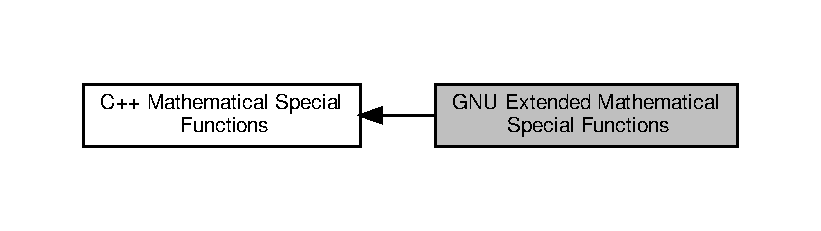
\includegraphics[width=350pt]{group__gnu__math__spec__func}
\end{center}
\end{figure}
\subsection*{Enumerations}
\begin{DoxyCompactItemize}
\item 
enum \{ \hyperlink{group__gnu__math__spec__func_ggad6c62dd86a596716cece6ac2d4cfd4b3a3f3a4942031777493cbc33f592c941c7}{\+\_\+\+\_\+gnu\+\_\+cxx\+::\+\_\+\+G\+L\+I\+B\+C\+X\+X\+\_\+\+J\+A\+C\+O\+B\+I\+\_\+\+SN}, 
\hyperlink{group__gnu__math__spec__func_ggad6c62dd86a596716cece6ac2d4cfd4b3a86d36c2efbbbfddcfb1e552853d72d65}{\+\_\+\+\_\+gnu\+\_\+cxx\+::\+\_\+\+G\+L\+I\+B\+C\+X\+X\+\_\+\+J\+A\+C\+O\+B\+I\+\_\+\+CN}, 
\hyperlink{group__gnu__math__spec__func_ggad6c62dd86a596716cece6ac2d4cfd4b3a4576182edcbe93595def76dd1e61e0f7}{\+\_\+\+\_\+gnu\+\_\+cxx\+::\+\_\+\+G\+L\+I\+B\+C\+X\+X\+\_\+\+J\+A\+C\+O\+B\+I\+\_\+\+DN}
 \}
\end{DoxyCompactItemize}
\subsection*{Functions}
\begin{DoxyCompactItemize}
\item 
{\footnotesize template$<$typename \+\_\+\+Tp $>$ }\\\+\_\+\+\_\+gnu\+\_\+cxx\+::\+\_\+\+\_\+promote\+\_\+fp\+\_\+t$<$ \+\_\+\+Tp $>$ \hyperlink{group__gnu__math__spec__func_ga53243cdb83abeb008fa90d8a098768af}{\+\_\+\+\_\+gnu\+\_\+cxx\+::airy\+\_\+ai} (\+\_\+\+Tp \+\_\+\+\_\+x)
\item 
{\footnotesize template$<$typename \+\_\+\+Tp $>$ }\\std\+::complex$<$ \+\_\+\+\_\+gnu\+\_\+cxx\+::\+\_\+\+\_\+promote\+\_\+fp\+\_\+t$<$ \+\_\+\+Tp $>$ $>$ \hyperlink{group__gnu__math__spec__func_gab61dcd6c20c602711544b39d2429038b}{\+\_\+\+\_\+gnu\+\_\+cxx\+::airy\+\_\+ai} (std\+::complex$<$ \+\_\+\+Tp $>$ \+\_\+\+\_\+x)
\item 
float \hyperlink{group__gnu__math__spec__func_gaf317ba724c44b3a8271fe341d9870173}{\+\_\+\+\_\+gnu\+\_\+cxx\+::airy\+\_\+aif} (float \+\_\+\+\_\+x)
\item 
long double \hyperlink{group__gnu__math__spec__func_ga800fdb61c672ae1831f4ca4250d657de}{\+\_\+\+\_\+gnu\+\_\+cxx\+::airy\+\_\+ail} (long double \+\_\+\+\_\+x)
\item 
{\footnotesize template$<$typename \+\_\+\+Tp $>$ }\\\+\_\+\+\_\+gnu\+\_\+cxx\+::\+\_\+\+\_\+promote\+\_\+fp\+\_\+t$<$ \+\_\+\+Tp $>$ \hyperlink{group__gnu__math__spec__func_ga812ca309bff1b0ae2bbe1183a0bc47d5}{\+\_\+\+\_\+gnu\+\_\+cxx\+::airy\+\_\+bi} (\+\_\+\+Tp \+\_\+\+\_\+x)
\item 
{\footnotesize template$<$typename \+\_\+\+Tp $>$ }\\std\+::complex$<$ \+\_\+\+\_\+gnu\+\_\+cxx\+::\+\_\+\+\_\+promote\+\_\+fp\+\_\+t$<$ \+\_\+\+Tp $>$ $>$ \hyperlink{group__gnu__math__spec__func_ga6dee14118a9bc3ccfa6f1d2b96b4be10}{\+\_\+\+\_\+gnu\+\_\+cxx\+::airy\+\_\+bi} (std\+::complex$<$ \+\_\+\+Tp $>$ \+\_\+\+\_\+x)
\item 
float \hyperlink{group__gnu__math__spec__func_ga2ade465827bdba7370abbcce78e54912}{\+\_\+\+\_\+gnu\+\_\+cxx\+::airy\+\_\+bif} (float \+\_\+\+\_\+x)
\item 
long double \hyperlink{group__gnu__math__spec__func_ga59240b3f40177e5187f3f194f624f0f8}{\+\_\+\+\_\+gnu\+\_\+cxx\+::airy\+\_\+bil} (long double \+\_\+\+\_\+x)
\item 
{\footnotesize template$<$typename \+\_\+\+Tp $>$ }\\\+\_\+\+\_\+gnu\+\_\+cxx\+::\+\_\+\+\_\+promote\+\_\+fp\+\_\+t$<$ \+\_\+\+Tp $>$ \hyperlink{group__gnu__math__spec__func_gaebe41d6ec250e8fcc213eee9b392fd5f}{\+\_\+\+\_\+gnu\+\_\+cxx\+::bernoulli} (unsigned int \+\_\+\+\_\+n)
\item 
float \hyperlink{group__gnu__math__spec__func_gabcd77f012ae74989c4bb9ca61978481d}{\+\_\+\+\_\+gnu\+\_\+cxx\+::bernoullif} (unsigned int \+\_\+\+\_\+n)
\item 
long double \hyperlink{group__gnu__math__spec__func_gaac8f04abfdd6b744d11cb73ec1f564b1}{\+\_\+\+\_\+gnu\+\_\+cxx\+::bernoullil} (unsigned int \+\_\+\+\_\+n)
\item 
{\footnotesize template$<$typename \+\_\+\+Tp $>$ }\\\+\_\+\+\_\+gnu\+\_\+cxx\+::\+\_\+\+\_\+promote\+\_\+fp\+\_\+t$<$ \+\_\+\+Tp $>$ \hyperlink{group__gnu__math__spec__func_ga2934ccfb8bbd5877efd369a3ecd9ac4d}{\+\_\+\+\_\+gnu\+\_\+cxx\+::bincoef} (unsigned int \+\_\+\+\_\+n, unsigned int \+\_\+\+\_\+k)
\item 
float \hyperlink{group__gnu__math__spec__func_ga20ff8c4c82808c78c299634d02f3f8bd}{\+\_\+\+\_\+gnu\+\_\+cxx\+::bincoeff} (unsigned int \+\_\+\+\_\+n, unsigned int \+\_\+\+\_\+k)
\item 
long double \hyperlink{group__gnu__math__spec__func_ga6874da4660b1ef35c03e28bf09e81796}{\+\_\+\+\_\+gnu\+\_\+cxx\+::bincoefl} (unsigned int \+\_\+\+\_\+n, unsigned int \+\_\+\+\_\+k)
\item 
{\footnotesize template$<$typename \+\_\+\+Tps , typename \+\_\+\+Tp $>$ }\\\+\_\+\+\_\+gnu\+\_\+cxx\+::\+\_\+\+\_\+promote\+\_\+fp\+\_\+t$<$ \+\_\+\+Tps, \+\_\+\+Tp $>$ \hyperlink{group__gnu__math__spec__func_gacf63ebbc67ea21d569cf510ed0da95fd}{\+\_\+\+\_\+gnu\+\_\+cxx\+::bose\+\_\+einstein} (\+\_\+\+Tps \+\_\+\+\_\+s, \+\_\+\+Tp \+\_\+\+\_\+x)
\item 
float \hyperlink{group__gnu__math__spec__func_gac1fb313fba5639d4168b6ee682507688}{\+\_\+\+\_\+gnu\+\_\+cxx\+::bose\+\_\+einsteinf} (float \+\_\+\+\_\+s, float \+\_\+\+\_\+x)
\item 
long double \hyperlink{group__gnu__math__spec__func_ga995c3ff580f81afb139f9cd50f445b48}{\+\_\+\+\_\+gnu\+\_\+cxx\+::bose\+\_\+einsteinl} (long double \+\_\+\+\_\+s, long double \+\_\+\+\_\+x)
\item 
{\footnotesize template$<$typename \+\_\+\+Tp $>$ }\\\+\_\+\+\_\+gnu\+\_\+cxx\+::\+\_\+\+\_\+promote\+\_\+fp\+\_\+t$<$ \+\_\+\+Tp $>$ \hyperlink{group__gnu__math__spec__func_gae35c0bc63248e3bcdb9b490477975eb4}{\+\_\+\+\_\+gnu\+\_\+cxx\+::chebyshev\+\_\+t} (unsigned int \+\_\+\+\_\+n, \+\_\+\+Tp \+\_\+\+\_\+x)
\item 
float \hyperlink{group__gnu__math__spec__func_gab8cdb55702d9c8b85af4ecc3d8c6a134}{\+\_\+\+\_\+gnu\+\_\+cxx\+::chebyshev\+\_\+tf} (unsigned int \+\_\+\+\_\+n, float \+\_\+\+\_\+x)
\item 
long double \hyperlink{group__gnu__math__spec__func_ga0c421700d244cdf58e3ac5ff267664d1}{\+\_\+\+\_\+gnu\+\_\+cxx\+::chebyshev\+\_\+tl} (unsigned int \+\_\+\+\_\+n, long double \+\_\+\+\_\+x)
\item 
{\footnotesize template$<$typename \+\_\+\+Tp $>$ }\\\+\_\+\+\_\+gnu\+\_\+cxx\+::\+\_\+\+\_\+promote\+\_\+fp\+\_\+t$<$ \+\_\+\+Tp $>$ \hyperlink{group__gnu__math__spec__func_gaea7ea830fe6be79ca84fba1bb94691a4}{\+\_\+\+\_\+gnu\+\_\+cxx\+::chebyshev\+\_\+u} (unsigned int \+\_\+\+\_\+n, \+\_\+\+Tp \+\_\+\+\_\+x)
\item 
float \hyperlink{group__gnu__math__spec__func_ga4b28c2a079eae2e9612c9902801ca256}{\+\_\+\+\_\+gnu\+\_\+cxx\+::chebyshev\+\_\+uf} (unsigned int \+\_\+\+\_\+n, float \+\_\+\+\_\+x)
\item 
long double \hyperlink{group__gnu__math__spec__func_ga11ec202d6aacafba1182e962ecf02978}{\+\_\+\+\_\+gnu\+\_\+cxx\+::chebyshev\+\_\+ul} (unsigned int \+\_\+\+\_\+n, long double \+\_\+\+\_\+x)
\item 
{\footnotesize template$<$typename \+\_\+\+Tp $>$ }\\\+\_\+\+\_\+gnu\+\_\+cxx\+::\+\_\+\+\_\+promote\+\_\+fp\+\_\+t$<$ \+\_\+\+Tp $>$ \hyperlink{group__gnu__math__spec__func_ga674e3d97204a74620eb0d408873aefb9}{\+\_\+\+\_\+gnu\+\_\+cxx\+::chebyshev\+\_\+v} (unsigned int \+\_\+\+\_\+n, \+\_\+\+Tp \+\_\+\+\_\+x)
\item 
float \hyperlink{group__gnu__math__spec__func_gaa9635a0da4bdeaa8060ae5cf03c3a12d}{\+\_\+\+\_\+gnu\+\_\+cxx\+::chebyshev\+\_\+vf} (unsigned int \+\_\+\+\_\+n, float \+\_\+\+\_\+x)
\item 
long double \hyperlink{group__gnu__math__spec__func_gae387ee1bfcd52555ad4d690f5888a078}{\+\_\+\+\_\+gnu\+\_\+cxx\+::chebyshev\+\_\+vl} (unsigned int \+\_\+\+\_\+n, long double \+\_\+\+\_\+x)
\item 
{\footnotesize template$<$typename \+\_\+\+Tp $>$ }\\\+\_\+\+\_\+gnu\+\_\+cxx\+::\+\_\+\+\_\+promote\+\_\+fp\+\_\+t$<$ \+\_\+\+Tp $>$ \hyperlink{group__gnu__math__spec__func_ga55ebf3cda76302bc6e0f173fc1c1425e}{\+\_\+\+\_\+gnu\+\_\+cxx\+::chebyshev\+\_\+w} (unsigned int \+\_\+\+\_\+n, \+\_\+\+Tp \+\_\+\+\_\+x)
\item 
float \hyperlink{group__gnu__math__spec__func_gae6d468cee53df584e40afe294127b090}{\+\_\+\+\_\+gnu\+\_\+cxx\+::chebyshev\+\_\+wf} (unsigned int \+\_\+\+\_\+n, float \+\_\+\+\_\+x)
\item 
long double \hyperlink{group__gnu__math__spec__func_ga1297dfd9b9a0f584435de7d83eb9e9c3}{\+\_\+\+\_\+gnu\+\_\+cxx\+::chebyshev\+\_\+wl} (unsigned int \+\_\+\+\_\+n, long double \+\_\+\+\_\+x)
\item 
{\footnotesize template$<$typename \+\_\+\+Tp $>$ }\\\+\_\+\+\_\+gnu\+\_\+cxx\+::\+\_\+\+\_\+promote\+\_\+fp\+\_\+t$<$ \+\_\+\+Tp $>$ \hyperlink{group__gnu__math__spec__func_ga7959ce3dea7f8d98b1dfee5715303f1c}{\+\_\+\+\_\+gnu\+\_\+cxx\+::clausen} (unsigned int \+\_\+\+\_\+m, \+\_\+\+Tp \+\_\+\+\_\+w)
\item 
{\footnotesize template$<$typename \+\_\+\+Tp $>$ }\\std\+::complex$<$ \+\_\+\+\_\+gnu\+\_\+cxx\+::\+\_\+\+\_\+promote\+\_\+fp\+\_\+t$<$ \+\_\+\+Tp $>$ $>$ \hyperlink{group__gnu__math__spec__func_ga4ffe44c8ee15518ac2577ba0aa94a99c}{\+\_\+\+\_\+gnu\+\_\+cxx\+::clausen} (unsigned int \+\_\+\+\_\+m, std\+::complex$<$ \+\_\+\+Tp $>$ \+\_\+\+\_\+w)
\item 
{\footnotesize template$<$typename \+\_\+\+Tp $>$ }\\\+\_\+\+\_\+gnu\+\_\+cxx\+::\+\_\+\+\_\+promote\+\_\+fp\+\_\+t$<$ \+\_\+\+Tp $>$ \hyperlink{group__gnu__math__spec__func_gabbdae75b253a0b19e8ae3d42c14f6be3}{\+\_\+\+\_\+gnu\+\_\+cxx\+::clausen\+\_\+c} (unsigned int \+\_\+\+\_\+m, \+\_\+\+Tp \+\_\+\+\_\+w)
\item 
float \hyperlink{group__gnu__math__spec__func_ga515b9b6bca8f97e696ac5be85a44b3bd}{\+\_\+\+\_\+gnu\+\_\+cxx\+::clausen\+\_\+cf} (unsigned int \+\_\+\+\_\+m, float \+\_\+\+\_\+w)
\item 
long double \hyperlink{group__gnu__math__spec__func_ga5ff89833dc529ca3de5099e1b9c8525f}{\+\_\+\+\_\+gnu\+\_\+cxx\+::clausen\+\_\+cl} (unsigned int \+\_\+\+\_\+m, long double \+\_\+\+\_\+w)
\item 
{\footnotesize template$<$typename \+\_\+\+Tp $>$ }\\\+\_\+\+\_\+gnu\+\_\+cxx\+::\+\_\+\+\_\+promote\+\_\+fp\+\_\+t$<$ \+\_\+\+Tp $>$ \hyperlink{group__gnu__math__spec__func_ga3ed0e444799410cda76ccbc62181ce0c}{\+\_\+\+\_\+gnu\+\_\+cxx\+::clausen\+\_\+s} (unsigned int \+\_\+\+\_\+m, \+\_\+\+Tp \+\_\+\+\_\+w)
\item 
float \hyperlink{group__gnu__math__spec__func_ga2308b5828b5a8003d16cfa0f90826f94}{\+\_\+\+\_\+gnu\+\_\+cxx\+::clausen\+\_\+sf} (unsigned int \+\_\+\+\_\+m, float \+\_\+\+\_\+w)
\item 
long double \hyperlink{group__gnu__math__spec__func_ga6eb205278e3807367b62e07c3f39d915}{\+\_\+\+\_\+gnu\+\_\+cxx\+::clausen\+\_\+sl} (unsigned int \+\_\+\+\_\+m, long double \+\_\+\+\_\+w)
\item 
float \hyperlink{group__gnu__math__spec__func_ga9e228490e55e7936f77ae7a5ef9821dc}{\+\_\+\+\_\+gnu\+\_\+cxx\+::clausenf} (unsigned int \+\_\+\+\_\+m, float \+\_\+\+\_\+w)
\item 
std\+::complex$<$ float $>$ \hyperlink{group__gnu__math__spec__func_ga769ee593c5f1c1d8148abb9bebe50821}{\+\_\+\+\_\+gnu\+\_\+cxx\+::clausenf} (unsigned int \+\_\+\+\_\+m, std\+::complex$<$ float $>$ \+\_\+\+\_\+w)
\item 
long double \hyperlink{group__gnu__math__spec__func_gaac0a4d039044c04cd26c9b8559c441fd}{\+\_\+\+\_\+gnu\+\_\+cxx\+::clausenl} (unsigned int \+\_\+\+\_\+m, long double \+\_\+\+\_\+w)
\item 
std\+::complex$<$ long double $>$ \hyperlink{group__gnu__math__spec__func_ga6e1e9929ace5a66d970c308554473a26}{\+\_\+\+\_\+gnu\+\_\+cxx\+::clausenl} (unsigned int \+\_\+\+\_\+m, std\+::complex$<$ long double $>$ \+\_\+\+\_\+w)
\item 
{\footnotesize template$<$typename \+\_\+\+Tk $>$ }\\\+\_\+\+\_\+gnu\+\_\+cxx\+::\+\_\+\+\_\+promote\+\_\+fp\+\_\+t$<$ \+\_\+\+Tk $>$ \hyperlink{group__gnu__math__spec__func_ga2c6b6c5a44ea00f0aed05c02f1072c31}{\+\_\+\+\_\+gnu\+\_\+cxx\+::comp\+\_\+ellint\+\_\+d} (\+\_\+\+Tk \+\_\+\+\_\+k)
\item 
float \hyperlink{group__gnu__math__spec__func_ga34ac6488b0e7531d5d4b7a8e31ff864e}{\+\_\+\+\_\+gnu\+\_\+cxx\+::comp\+\_\+ellint\+\_\+df} (float \+\_\+\+\_\+k)
\item 
long double \hyperlink{group__gnu__math__spec__func_ga494931ec0a271b79f1fdcfdf929e3138}{\+\_\+\+\_\+gnu\+\_\+cxx\+::comp\+\_\+ellint\+\_\+dl} (long double \+\_\+\+\_\+k)
\item 
float \hyperlink{group__gnu__math__spec__func_ga55ae30b4f8ff15017d18a80050e14e38}{\+\_\+\+\_\+gnu\+\_\+cxx\+::comp\+\_\+ellint\+\_\+rf} (float \+\_\+\+\_\+x, float \+\_\+\+\_\+y)
\item 
long double \hyperlink{group__gnu__math__spec__func_gae1d468487f1711e91719a9c6392f3c35}{\+\_\+\+\_\+gnu\+\_\+cxx\+::comp\+\_\+ellint\+\_\+rf} (long double \+\_\+\+\_\+x, long double \+\_\+\+\_\+y)
\item 
{\footnotesize template$<$typename \+\_\+\+Tx , typename \+\_\+\+Ty $>$ }\\\+\_\+\+\_\+gnu\+\_\+cxx\+::\+\_\+\+\_\+promote\+\_\+fp\+\_\+t$<$ \+\_\+\+Tx, \+\_\+\+Ty $>$ \hyperlink{group__gnu__math__spec__func_ga78dc5f41ec8b69ed822612a72d326109}{\+\_\+\+\_\+gnu\+\_\+cxx\+::comp\+\_\+ellint\+\_\+rf} (\+\_\+\+Tx \+\_\+\+\_\+x, \+\_\+\+Ty \+\_\+\+\_\+y)
\item 
float \hyperlink{group__gnu__math__spec__func_ga978f8eec6e5edc918b243925dbacb65b}{\+\_\+\+\_\+gnu\+\_\+cxx\+::comp\+\_\+ellint\+\_\+rg} (float \+\_\+\+\_\+x, float \+\_\+\+\_\+y)
\item 
long double \hyperlink{group__gnu__math__spec__func_gaca5fa8ee8125afc8f35ec6b27806e873}{\+\_\+\+\_\+gnu\+\_\+cxx\+::comp\+\_\+ellint\+\_\+rg} (long double \+\_\+\+\_\+x, long double \+\_\+\+\_\+y)
\item 
{\footnotesize template$<$typename \+\_\+\+Tx , typename \+\_\+\+Ty $>$ }\\\+\_\+\+\_\+gnu\+\_\+cxx\+::\+\_\+\+\_\+promote\+\_\+fp\+\_\+t$<$ \+\_\+\+Tx, \+\_\+\+Ty $>$ \hyperlink{group__gnu__math__spec__func_gad0ab2cfa6c4669440c47ab53cfa332ec}{\+\_\+\+\_\+gnu\+\_\+cxx\+::comp\+\_\+ellint\+\_\+rg} (\+\_\+\+Tx \+\_\+\+\_\+x, \+\_\+\+Ty \+\_\+\+\_\+y)
\item 
{\footnotesize template$<$typename \+\_\+\+Tpa , typename \+\_\+\+Tpc , typename \+\_\+\+Tp $>$ }\\\+\_\+\+\_\+gnu\+\_\+cxx\+::\+\_\+\+\_\+promote\+\_\+fp\+\_\+t$<$ \+\_\+\+Tpa, \+\_\+\+Tpc, \+\_\+\+Tp $>$ \hyperlink{group__gnu__math__spec__func_ga5e71f453c84b767792dc26ffda96f8fb}{\+\_\+\+\_\+gnu\+\_\+cxx\+::conf\+\_\+hyperg} (\+\_\+\+Tpa \+\_\+\+\_\+a, \+\_\+\+Tpc \+\_\+\+\_\+c, \+\_\+\+Tp \+\_\+\+\_\+x)
\item 
{\footnotesize template$<$typename \+\_\+\+Tpc , typename \+\_\+\+Tp $>$ }\\\+\_\+\+\_\+gnu\+\_\+cxx\+::\+\_\+\+\_\+promote\+\_\+2$<$ \+\_\+\+Tpc, \+\_\+\+Tp $>$\+::\+\_\+\+\_\+type \hyperlink{group__gnu__math__spec__func_gab923b5a9e67469a5145d7bfcb20b3396}{\+\_\+\+\_\+gnu\+\_\+cxx\+::conf\+\_\+hyperg\+\_\+lim} (\+\_\+\+Tpc \+\_\+\+\_\+c, \+\_\+\+Tp \+\_\+\+\_\+x)
\item 
float \hyperlink{group__gnu__math__spec__func_ga609879a370bc4e9fc70563806bc49cb9}{\+\_\+\+\_\+gnu\+\_\+cxx\+::conf\+\_\+hyperg\+\_\+limf} (float \+\_\+\+\_\+c, float \+\_\+\+\_\+x)
\item 
long double \hyperlink{group__gnu__math__spec__func_ga367be9b77eb1f9ccc2971d5300da48d1}{\+\_\+\+\_\+gnu\+\_\+cxx\+::conf\+\_\+hyperg\+\_\+liml} (long double \+\_\+\+\_\+c, long double \+\_\+\+\_\+x)
\item 
float \hyperlink{group__gnu__math__spec__func_gabd18e600aa78c3f2b2f835039506c810}{\+\_\+\+\_\+gnu\+\_\+cxx\+::conf\+\_\+hypergf} (float \+\_\+\+\_\+a, float \+\_\+\+\_\+c, float \+\_\+\+\_\+x)
\item 
long double \hyperlink{group__gnu__math__spec__func_ga0a9853f30d8fa515a12cd45a92da832e}{\+\_\+\+\_\+gnu\+\_\+cxx\+::conf\+\_\+hypergl} (long double \+\_\+\+\_\+a, long double \+\_\+\+\_\+c, long double \+\_\+\+\_\+x)
\item 
{\footnotesize template$<$typename \+\_\+\+Tp $>$ }\\\+\_\+\+\_\+gnu\+\_\+cxx\+::\+\_\+\+\_\+promote\+\_\+fp\+\_\+t$<$ \+\_\+\+Tp $>$ \hyperlink{group__gnu__math__spec__func_ga05f183d57b1726136ba9795ba1b158c5}{\+\_\+\+\_\+gnu\+\_\+cxx\+::cos\+\_\+pi} (\+\_\+\+Tp \+\_\+\+\_\+x)
\item 
float \hyperlink{group__gnu__math__spec__func_gaddcae99c1572af6fa1d79b9cfa053033}{\+\_\+\+\_\+gnu\+\_\+cxx\+::cos\+\_\+pif} (float \+\_\+\+\_\+x)
\item 
long double \hyperlink{group__gnu__math__spec__func_ga9b6816c0abf30fd88417d79a33cb5465}{\+\_\+\+\_\+gnu\+\_\+cxx\+::cos\+\_\+pil} (long double \+\_\+\+\_\+x)
\item 
{\footnotesize template$<$typename \+\_\+\+Tp $>$ }\\\+\_\+\+\_\+gnu\+\_\+cxx\+::\+\_\+\+\_\+promote\+\_\+fp\+\_\+t$<$ \+\_\+\+Tp $>$ \hyperlink{group__gnu__math__spec__func_ga633224563637e80a4cda93863a693ad6}{\+\_\+\+\_\+gnu\+\_\+cxx\+::cosh\+\_\+pi} (\+\_\+\+Tp \+\_\+\+\_\+x)
\item 
float \hyperlink{group__gnu__math__spec__func_ga79a2f5c9da96b5ea6c663d6efca24944}{\+\_\+\+\_\+gnu\+\_\+cxx\+::cosh\+\_\+pif} (float \+\_\+\+\_\+x)
\item 
long double \hyperlink{group__gnu__math__spec__func_gab7bf4f591dd35af2bdb88a8219f5e248}{\+\_\+\+\_\+gnu\+\_\+cxx\+::cosh\+\_\+pil} (long double \+\_\+\+\_\+x)
\item 
{\footnotesize template$<$typename \+\_\+\+Tp $>$ }\\\+\_\+\+\_\+gnu\+\_\+cxx\+::\+\_\+\+\_\+promote\+\_\+fp\+\_\+t$<$ \+\_\+\+Tp $>$ \hyperlink{group__gnu__math__spec__func_ga901c23871fded7d4467a864fe06bbf07}{\+\_\+\+\_\+gnu\+\_\+cxx\+::coshint} (\+\_\+\+Tp \+\_\+\+\_\+x)
\item 
float \hyperlink{group__gnu__math__spec__func_ga1af4d48209169967a836bd97e625a128}{\+\_\+\+\_\+gnu\+\_\+cxx\+::coshintf} (float \+\_\+\+\_\+x)
\item 
long double \hyperlink{group__gnu__math__spec__func_ga6d24ab53fad13d421f07d9a9a509de14}{\+\_\+\+\_\+gnu\+\_\+cxx\+::coshintl} (long double \+\_\+\+\_\+x)
\item 
{\footnotesize template$<$typename \+\_\+\+Tp $>$ }\\\+\_\+\+\_\+gnu\+\_\+cxx\+::\+\_\+\+\_\+promote\+\_\+fp\+\_\+t$<$ \+\_\+\+Tp $>$ \hyperlink{group__gnu__math__spec__func_ga06eed76a045a73ad72fcf4ad00b05f96}{\+\_\+\+\_\+gnu\+\_\+cxx\+::cosint} (\+\_\+\+Tp \+\_\+\+\_\+x)
\item 
float \hyperlink{group__gnu__math__spec__func_ga87202351dc97d2c69e42bf58f911fb5a}{\+\_\+\+\_\+gnu\+\_\+cxx\+::cosintf} (float \+\_\+\+\_\+x)
\item 
long double \hyperlink{group__gnu__math__spec__func_ga5f01f17ae8859129860118b09d51791c}{\+\_\+\+\_\+gnu\+\_\+cxx\+::cosintl} (long double \+\_\+\+\_\+x)
\item 
{\footnotesize template$<$typename \+\_\+\+Tpnu , typename \+\_\+\+Tp $>$ }\\std\+::complex$<$ \+\_\+\+\_\+gnu\+\_\+cxx\+::\+\_\+\+\_\+promote\+\_\+fp\+\_\+t$<$ \+\_\+\+Tpnu, \+\_\+\+Tp $>$ $>$ \hyperlink{group__gnu__math__spec__func_gafa5ad1cfd4cc30caaeb06bdab71e600b}{\+\_\+\+\_\+gnu\+\_\+cxx\+::cyl\+\_\+hankel\+\_\+1} (\+\_\+\+Tpnu \+\_\+\+\_\+nu, \+\_\+\+Tp \+\_\+\+\_\+z)
\item 
{\footnotesize template$<$typename \+\_\+\+Tpnu , typename \+\_\+\+Tp $>$ }\\std\+::complex$<$ \+\_\+\+\_\+gnu\+\_\+cxx\+::\+\_\+\+\_\+promote\+\_\+fp\+\_\+t$<$ \+\_\+\+Tpnu, \+\_\+\+Tp $>$ $>$ \hyperlink{group__gnu__math__spec__func_ga0f0b05c483ed1d713ef9a96e844c1979}{\+\_\+\+\_\+gnu\+\_\+cxx\+::cyl\+\_\+hankel\+\_\+1} (std\+::complex$<$ \+\_\+\+Tpnu $>$ \+\_\+\+\_\+nu, std\+::complex$<$ \+\_\+\+Tp $>$ \+\_\+\+\_\+x)
\item 
std\+::complex$<$ float $>$ \hyperlink{group__gnu__math__spec__func_ga89758ed03e56567baa62b90cc4784f71}{\+\_\+\+\_\+gnu\+\_\+cxx\+::cyl\+\_\+hankel\+\_\+1f} (float \+\_\+\+\_\+nu, float \+\_\+\+\_\+z)
\item 
std\+::complex$<$ float $>$ \hyperlink{group__gnu__math__spec__func_ga810e021a3f11c1b2253c15c6f4d41143}{\+\_\+\+\_\+gnu\+\_\+cxx\+::cyl\+\_\+hankel\+\_\+1f} (std\+::complex$<$ float $>$ \+\_\+\+\_\+nu, std\+::complex$<$ float $>$ \+\_\+\+\_\+x)
\item 
std\+::complex$<$ long double $>$ \hyperlink{group__gnu__math__spec__func_gacb49c66b4267fbc56906db02f14365f2}{\+\_\+\+\_\+gnu\+\_\+cxx\+::cyl\+\_\+hankel\+\_\+1l} (long double \+\_\+\+\_\+nu, long double \+\_\+\+\_\+z)
\item 
std\+::complex$<$ long double $>$ \hyperlink{group__gnu__math__spec__func_ga6900f79ec70673bcb001538aec74e07c}{\+\_\+\+\_\+gnu\+\_\+cxx\+::cyl\+\_\+hankel\+\_\+1l} (std\+::complex$<$ long double $>$ \+\_\+\+\_\+nu, std\+::complex$<$ long double $>$ \+\_\+\+\_\+x)
\item 
{\footnotesize template$<$typename \+\_\+\+Tpnu , typename \+\_\+\+Tp $>$ }\\std\+::complex$<$ \+\_\+\+\_\+gnu\+\_\+cxx\+::\+\_\+\+\_\+promote\+\_\+fp\+\_\+t$<$ \+\_\+\+Tpnu, \+\_\+\+Tp $>$ $>$ \hyperlink{group__gnu__math__spec__func_ga6c1d2d390e547ded9e0f4cc46395d90c}{\+\_\+\+\_\+gnu\+\_\+cxx\+::cyl\+\_\+hankel\+\_\+2} (\+\_\+\+Tpnu \+\_\+\+\_\+nu, \+\_\+\+Tp \+\_\+\+\_\+z)
\item 
{\footnotesize template$<$typename \+\_\+\+Tpnu , typename \+\_\+\+Tp $>$ }\\std\+::complex$<$ \+\_\+\+\_\+gnu\+\_\+cxx\+::\+\_\+\+\_\+promote\+\_\+fp\+\_\+t$<$ \+\_\+\+Tpnu, \+\_\+\+Tp $>$ $>$ \hyperlink{group__gnu__math__spec__func_ga378002c9d6cb4f64683bdb128da1df47}{\+\_\+\+\_\+gnu\+\_\+cxx\+::cyl\+\_\+hankel\+\_\+2} (std\+::complex$<$ \+\_\+\+Tpnu $>$ \+\_\+\+\_\+nu, std\+::complex$<$ \+\_\+\+Tp $>$ \+\_\+\+\_\+x)
\item 
std\+::complex$<$ float $>$ \hyperlink{group__gnu__math__spec__func_ga2b75361870975c47d57bed71b4064ce7}{\+\_\+\+\_\+gnu\+\_\+cxx\+::cyl\+\_\+hankel\+\_\+2f} (float \+\_\+\+\_\+nu, float \+\_\+\+\_\+z)
\item 
std\+::complex$<$ float $>$ \hyperlink{group__gnu__math__spec__func_gae21f9d09b937eaf9729982da5a382f20}{\+\_\+\+\_\+gnu\+\_\+cxx\+::cyl\+\_\+hankel\+\_\+2f} (std\+::complex$<$ float $>$ \+\_\+\+\_\+nu, std\+::complex$<$ float $>$ \+\_\+\+\_\+x)
\item 
std\+::complex$<$ long double $>$ \hyperlink{group__gnu__math__spec__func_ga4babb91ca6906f237e8bd1f0f1a10509}{\+\_\+\+\_\+gnu\+\_\+cxx\+::cyl\+\_\+hankel\+\_\+2l} (long double \+\_\+\+\_\+nu, long double \+\_\+\+\_\+z)
\item 
std\+::complex$<$ long double $>$ \hyperlink{group__gnu__math__spec__func_ga1ac6434925254bd02e108f5a4e52b34d}{\+\_\+\+\_\+gnu\+\_\+cxx\+::cyl\+\_\+hankel\+\_\+2l} (std\+::complex$<$ long double $>$ \+\_\+\+\_\+nu, std\+::complex$<$ long double $>$ \+\_\+\+\_\+x)
\item 
{\footnotesize template$<$typename \+\_\+\+Tp $>$ }\\\+\_\+\+\_\+gnu\+\_\+cxx\+::\+\_\+\+\_\+promote\+\_\+fp\+\_\+t$<$ \+\_\+\+Tp $>$ \hyperlink{group__gnu__math__spec__func_ga0623ddcbfdce696781e19648fde6f33a}{\+\_\+\+\_\+gnu\+\_\+cxx\+::dawson} (\+\_\+\+Tp \+\_\+\+\_\+x)
\item 
float \hyperlink{group__gnu__math__spec__func_ga0a1b8e6760b8c7869127d41d96209318}{\+\_\+\+\_\+gnu\+\_\+cxx\+::dawsonf} (float \+\_\+\+\_\+x)
\item 
long double \hyperlink{group__gnu__math__spec__func_ga6647a7444ff9c7c1f2a8ed36761bfeb2}{\+\_\+\+\_\+gnu\+\_\+cxx\+::dawsonl} (long double \+\_\+\+\_\+x)
\item 
{\footnotesize template$<$typename \+\_\+\+Tp $>$ }\\\+\_\+\+\_\+gnu\+\_\+cxx\+::\+\_\+\+\_\+promote\+\_\+fp\+\_\+t$<$ \+\_\+\+Tp $>$ \hyperlink{group__gnu__math__spec__func_ga7a95a3cb9a53aca2a1ff9752ce9d5e3c}{\+\_\+\+\_\+gnu\+\_\+cxx\+::dilog} (\+\_\+\+Tp \+\_\+\+\_\+x)
\item 
float \hyperlink{group__gnu__math__spec__func_ga901091e0e7ce7d6113ae6a86f4865a92}{\+\_\+\+\_\+gnu\+\_\+cxx\+::dilogf} (float \+\_\+\+\_\+x)
\item 
long double \hyperlink{group__gnu__math__spec__func_gae90c13ee690ebaf10a18a900fe2646f9}{\+\_\+\+\_\+gnu\+\_\+cxx\+::dilogl} (long double \+\_\+\+\_\+x)
\item 
{\footnotesize template$<$typename \+\_\+\+Tp $>$ }\\\+\_\+\+Tp \hyperlink{group__gnu__math__spec__func_ga87466a2d429a2815d794acc21c882b08}{\+\_\+\+\_\+gnu\+\_\+cxx\+::dirichlet\+\_\+beta} (\+\_\+\+Tp \+\_\+\+\_\+s)
\item 
float \hyperlink{group__gnu__math__spec__func_ga9bb40e20b18e3eb822e70af955940830}{\+\_\+\+\_\+gnu\+\_\+cxx\+::dirichlet\+\_\+betaf} (float \+\_\+\+\_\+s)
\item 
long double \hyperlink{group__gnu__math__spec__func_gaed6fd85a4577f4de66d74742a1850a13}{\+\_\+\+\_\+gnu\+\_\+cxx\+::dirichlet\+\_\+betal} (long double \+\_\+\+\_\+s)
\item 
{\footnotesize template$<$typename \+\_\+\+Tp $>$ }\\\+\_\+\+Tp \hyperlink{group__gnu__math__spec__func_gae46e26e4107675d285c79a2d6202e6c7}{\+\_\+\+\_\+gnu\+\_\+cxx\+::dirichlet\+\_\+eta} (\+\_\+\+Tp \+\_\+\+\_\+s)
\item 
float \hyperlink{group__gnu__math__spec__func_ga6f05d076600b1de9193e586cf89547c9}{\+\_\+\+\_\+gnu\+\_\+cxx\+::dirichlet\+\_\+etaf} (float \+\_\+\+\_\+s)
\item 
long double \hyperlink{group__gnu__math__spec__func_ga408e2267b648f29445522dbafb7a0e1a}{\+\_\+\+\_\+gnu\+\_\+cxx\+::dirichlet\+\_\+etal} (long double \+\_\+\+\_\+s)
\item 
{\footnotesize template$<$typename \+\_\+\+Tp $>$ }\\\+\_\+\+Tp \hyperlink{group__gnu__math__spec__func_ga06842a81bdcabf9c62252dde992d42ee}{\+\_\+\+\_\+gnu\+\_\+cxx\+::dirichlet\+\_\+lambda} (\+\_\+\+Tp \+\_\+\+\_\+s)
\item 
float \hyperlink{group__gnu__math__spec__func_gaafd3ca6b0d71d55d3835536396eece8f}{\+\_\+\+\_\+gnu\+\_\+cxx\+::dirichlet\+\_\+lambdaf} (float \+\_\+\+\_\+s)
\item 
long double \hyperlink{group__gnu__math__spec__func_gab28d06c4e3c7457f1fa3663168678fb2}{\+\_\+\+\_\+gnu\+\_\+cxx\+::dirichlet\+\_\+lambdal} (long double \+\_\+\+\_\+s)
\item 
{\footnotesize template$<$typename \+\_\+\+Tp $>$ }\\\+\_\+\+\_\+gnu\+\_\+cxx\+::\+\_\+\+\_\+promote\+\_\+fp\+\_\+t$<$ \+\_\+\+Tp $>$ \hyperlink{group__gnu__math__spec__func_ga08c31a5dd1686a7633b46f923c47af46}{\+\_\+\+\_\+gnu\+\_\+cxx\+::double\+\_\+factorial} (int \+\_\+\+\_\+n)
\item 
float \hyperlink{group__gnu__math__spec__func_ga85ec284e603f32d18970bbdbb12d5150}{\+\_\+\+\_\+gnu\+\_\+cxx\+::double\+\_\+factorialf} (int \+\_\+\+\_\+n)
\item 
long double \hyperlink{group__gnu__math__spec__func_ga0366730a4a775256217ef1cd9d0c3a04}{\+\_\+\+\_\+gnu\+\_\+cxx\+::double\+\_\+factoriall} (int \+\_\+\+\_\+n)
\item 
{\footnotesize template$<$typename \+\_\+\+Tk , typename \+\_\+\+Tp , typename \+\_\+\+Ta , typename \+\_\+\+Tb $>$ }\\\+\_\+\+\_\+gnu\+\_\+cxx\+::\+\_\+\+\_\+promote\+\_\+fp\+\_\+t$<$ \+\_\+\+Tk, \+\_\+\+Tp, \+\_\+\+Ta, \+\_\+\+Tb $>$ \hyperlink{group__gnu__math__spec__func_ga45ad61f29827bcf27d05ead27490fe84}{\+\_\+\+\_\+gnu\+\_\+cxx\+::ellint\+\_\+cel} (\+\_\+\+Tk \+\_\+\+\_\+k\+\_\+c, \+\_\+\+Tp \+\_\+\+\_\+p, \+\_\+\+Ta \+\_\+\+\_\+a, \+\_\+\+Tb \+\_\+\+\_\+b)
\item 
float \hyperlink{group__gnu__math__spec__func_ga6d8fbef7853cf37de11278b1ff7127e8}{\+\_\+\+\_\+gnu\+\_\+cxx\+::ellint\+\_\+celf} (float \+\_\+\+\_\+k\+\_\+c, float \+\_\+\+\_\+p, float \+\_\+\+\_\+a, float \+\_\+\+\_\+b)
\item 
long double \hyperlink{group__gnu__math__spec__func_gaa5add699fb2b4b02e63f8725a3a79750}{\+\_\+\+\_\+gnu\+\_\+cxx\+::ellint\+\_\+cell} (long double \+\_\+\+\_\+k\+\_\+c, long double \+\_\+\+\_\+p, long double \+\_\+\+\_\+a, long double \+\_\+\+\_\+b)
\item 
{\footnotesize template$<$typename \+\_\+\+Tk , typename \+\_\+\+Tphi $>$ }\\\+\_\+\+\_\+gnu\+\_\+cxx\+::\+\_\+\+\_\+promote\+\_\+fp\+\_\+t$<$ \+\_\+\+Tk, \+\_\+\+Tphi $>$ \hyperlink{group__gnu__math__spec__func_ga71785ba6bad83f009cb2dc4d2d574194}{\+\_\+\+\_\+gnu\+\_\+cxx\+::ellint\+\_\+d} (\+\_\+\+Tk \+\_\+\+\_\+k, \+\_\+\+Tphi \+\_\+\+\_\+phi)
\item 
float \hyperlink{group__gnu__math__spec__func_ga02ed50be21fdd84ad6bed003f94a9e69}{\+\_\+\+\_\+gnu\+\_\+cxx\+::ellint\+\_\+df} (float \+\_\+\+\_\+k, float \+\_\+\+\_\+phi)
\item 
long double \hyperlink{group__gnu__math__spec__func_gaa34bcb8e316f2e8b2b2bf48cd89abd98}{\+\_\+\+\_\+gnu\+\_\+cxx\+::ellint\+\_\+dl} (long double \+\_\+\+\_\+k, long double \+\_\+\+\_\+phi)
\item 
{\footnotesize template$<$typename \+\_\+\+Tp , typename \+\_\+\+Tk $>$ }\\\+\_\+\+\_\+gnu\+\_\+cxx\+::\+\_\+\+\_\+promote\+\_\+fp\+\_\+t$<$ \+\_\+\+Tp, \+\_\+\+Tk $>$ \hyperlink{group__gnu__math__spec__func_gac012a02a3d206b2f2a0638ffd3693b83}{\+\_\+\+\_\+gnu\+\_\+cxx\+::ellint\+\_\+el1} (\+\_\+\+Tp \+\_\+\+\_\+x, \+\_\+\+Tk \+\_\+\+\_\+k\+\_\+c)
\item 
float \hyperlink{group__gnu__math__spec__func_ga8d8342bb4f42c7fe09b5589c54d4e713}{\+\_\+\+\_\+gnu\+\_\+cxx\+::ellint\+\_\+el1f} (float \+\_\+\+\_\+x, float \+\_\+\+\_\+k\+\_\+c)
\item 
long double \hyperlink{group__gnu__math__spec__func_gaeed1201e421be410460739048cba5cd8}{\+\_\+\+\_\+gnu\+\_\+cxx\+::ellint\+\_\+el1l} (long double \+\_\+\+\_\+x, long double \+\_\+\+\_\+k\+\_\+c)
\item 
{\footnotesize template$<$typename \+\_\+\+Tp , typename \+\_\+\+Tk , typename \+\_\+\+Ta , typename \+\_\+\+Tb $>$ }\\\+\_\+\+\_\+gnu\+\_\+cxx\+::\+\_\+\+\_\+promote\+\_\+fp\+\_\+t$<$ \+\_\+\+Tp, \+\_\+\+Tk, \+\_\+\+Ta, \+\_\+\+Tb $>$ \hyperlink{group__gnu__math__spec__func_ga43159d9468e4e31a0fbe391561f195be}{\+\_\+\+\_\+gnu\+\_\+cxx\+::ellint\+\_\+el2} (\+\_\+\+Tp \+\_\+\+\_\+x, \+\_\+\+Tk \+\_\+\+\_\+k\+\_\+c, \+\_\+\+Ta \+\_\+\+\_\+a, \+\_\+\+Tb \+\_\+\+\_\+b)
\item 
float \hyperlink{group__gnu__math__spec__func_ga0bf7469fe7ac92e9a2ffa0f92ea62248}{\+\_\+\+\_\+gnu\+\_\+cxx\+::ellint\+\_\+el2f} (float \+\_\+\+\_\+x, float \+\_\+\+\_\+k\+\_\+c, float \+\_\+\+\_\+a, float \+\_\+\+\_\+b)
\item 
long double \hyperlink{group__gnu__math__spec__func_ga491439a09e6000659444f52dc3c9f215}{\+\_\+\+\_\+gnu\+\_\+cxx\+::ellint\+\_\+el2l} (long double \+\_\+\+\_\+x, long double \+\_\+\+\_\+k\+\_\+c, long double \+\_\+\+\_\+a, long double \+\_\+\+\_\+b)
\item 
{\footnotesize template$<$typename \+\_\+\+Tx , typename \+\_\+\+Tk , typename \+\_\+\+Tp $>$ }\\\+\_\+\+\_\+gnu\+\_\+cxx\+::\+\_\+\+\_\+promote\+\_\+fp\+\_\+t$<$ \+\_\+\+Tx, \+\_\+\+Tk, \+\_\+\+Tp $>$ \hyperlink{group__gnu__math__spec__func_ga57b418ec87f207cdd1c9e5fa48b29333}{\+\_\+\+\_\+gnu\+\_\+cxx\+::ellint\+\_\+el3} (\+\_\+\+Tx \+\_\+\+\_\+x, \+\_\+\+Tk \+\_\+\+\_\+k\+\_\+c, \+\_\+\+Tp \+\_\+\+\_\+p)
\item 
float \hyperlink{group__gnu__math__spec__func_ga66131a8ecc14b5228a73a01121f60a35}{\+\_\+\+\_\+gnu\+\_\+cxx\+::ellint\+\_\+el3f} (float \+\_\+\+\_\+x, float \+\_\+\+\_\+k\+\_\+c, float \+\_\+\+\_\+p)
\item 
long double \hyperlink{group__gnu__math__spec__func_ga0d90e66f799a2ebe4bec43eef0d53355}{\+\_\+\+\_\+gnu\+\_\+cxx\+::ellint\+\_\+el3l} (long double \+\_\+\+\_\+x, long double \+\_\+\+\_\+k\+\_\+c, long double \+\_\+\+\_\+p)
\item 
{\footnotesize template$<$typename \+\_\+\+Tp , typename \+\_\+\+Up $>$ }\\\+\_\+\+\_\+gnu\+\_\+cxx\+::\+\_\+\+\_\+promote\+\_\+fp\+\_\+t$<$ \+\_\+\+Tp, \+\_\+\+Up $>$ \hyperlink{group__gnu__math__spec__func_ga21b90daf6c8d705b052304905809d2db}{\+\_\+\+\_\+gnu\+\_\+cxx\+::ellint\+\_\+rc} (\+\_\+\+Tp \+\_\+\+\_\+x, \+\_\+\+Up \+\_\+\+\_\+y)
\item 
float \hyperlink{group__gnu__math__spec__func_gaad5316092224ec3d92b66e79ef266adf}{\+\_\+\+\_\+gnu\+\_\+cxx\+::ellint\+\_\+rcf} (float \+\_\+\+\_\+x, float \+\_\+\+\_\+y)
\item 
long double \hyperlink{group__gnu__math__spec__func_ga9b2f1cdeacd3615c702a77d995a0129c}{\+\_\+\+\_\+gnu\+\_\+cxx\+::ellint\+\_\+rcl} (long double \+\_\+\+\_\+x, long double \+\_\+\+\_\+y)
\item 
{\footnotesize template$<$typename \+\_\+\+Tp , typename \+\_\+\+Up , typename \+\_\+\+Vp $>$ }\\\+\_\+\+\_\+gnu\+\_\+cxx\+::\+\_\+\+\_\+promote\+\_\+fp\+\_\+t$<$ \+\_\+\+Tp, \+\_\+\+Up, \+\_\+\+Vp $>$ \hyperlink{group__gnu__math__spec__func_ga6467a19028332392df825e232a97139f}{\+\_\+\+\_\+gnu\+\_\+cxx\+::ellint\+\_\+rd} (\+\_\+\+Tp \+\_\+\+\_\+x, \+\_\+\+Up \+\_\+\+\_\+y, \+\_\+\+Vp \+\_\+\+\_\+z)
\item 
float \hyperlink{group__gnu__math__spec__func_ga52e7cc797b9d199b7468cdbec6505357}{\+\_\+\+\_\+gnu\+\_\+cxx\+::ellint\+\_\+rdf} (float \+\_\+\+\_\+x, float \+\_\+\+\_\+y, float \+\_\+\+\_\+z)
\item 
long double \hyperlink{group__gnu__math__spec__func_ga68a38a5f320a7184cec4b120ddef6a65}{\+\_\+\+\_\+gnu\+\_\+cxx\+::ellint\+\_\+rdl} (long double \+\_\+\+\_\+x, long double \+\_\+\+\_\+y, long double \+\_\+\+\_\+z)
\item 
{\footnotesize template$<$typename \+\_\+\+Tp , typename \+\_\+\+Up , typename \+\_\+\+Vp $>$ }\\\+\_\+\+\_\+gnu\+\_\+cxx\+::\+\_\+\+\_\+promote\+\_\+fp\+\_\+t$<$ \+\_\+\+Tp, \+\_\+\+Up, \+\_\+\+Vp $>$ \hyperlink{group__gnu__math__spec__func_ga9242fbc43bd340e0def2a6f15b755c1c}{\+\_\+\+\_\+gnu\+\_\+cxx\+::ellint\+\_\+rf} (\+\_\+\+Tp \+\_\+\+\_\+x, \+\_\+\+Up \+\_\+\+\_\+y, \+\_\+\+Vp \+\_\+\+\_\+z)
\item 
float \hyperlink{group__gnu__math__spec__func_ga39acf5c69a85f9b687478b32847156da}{\+\_\+\+\_\+gnu\+\_\+cxx\+::ellint\+\_\+rff} (float \+\_\+\+\_\+x, float \+\_\+\+\_\+y, float \+\_\+\+\_\+z)
\item 
long double \hyperlink{group__gnu__math__spec__func_ga38dd36b3db5bbe5da516d0cbe3ff1f21}{\+\_\+\+\_\+gnu\+\_\+cxx\+::ellint\+\_\+rfl} (long double \+\_\+\+\_\+x, long double \+\_\+\+\_\+y, long double \+\_\+\+\_\+z)
\item 
{\footnotesize template$<$typename \+\_\+\+Tp , typename \+\_\+\+Up , typename \+\_\+\+Vp $>$ }\\\+\_\+\+\_\+gnu\+\_\+cxx\+::\+\_\+\+\_\+promote\+\_\+fp\+\_\+t$<$ \+\_\+\+Tp, \+\_\+\+Up, \+\_\+\+Vp $>$ \hyperlink{group__gnu__math__spec__func_gab525116e1b311da90e2745366ac314eb}{\+\_\+\+\_\+gnu\+\_\+cxx\+::ellint\+\_\+rg} (\+\_\+\+Tp \+\_\+\+\_\+x, \+\_\+\+Up \+\_\+\+\_\+y, \+\_\+\+Vp \+\_\+\+\_\+z)
\item 
float \hyperlink{group__gnu__math__spec__func_ga7a4ab348bf312a3425501ac8a3d16494}{\+\_\+\+\_\+gnu\+\_\+cxx\+::ellint\+\_\+rgf} (float \+\_\+\+\_\+x, float \+\_\+\+\_\+y, float \+\_\+\+\_\+z)
\item 
long double \hyperlink{group__gnu__math__spec__func_ga563455d515ed845988552432108a21be}{\+\_\+\+\_\+gnu\+\_\+cxx\+::ellint\+\_\+rgl} (long double \+\_\+\+\_\+x, long double \+\_\+\+\_\+y, long double \+\_\+\+\_\+z)
\item 
{\footnotesize template$<$typename \+\_\+\+Tp , typename \+\_\+\+Up , typename \+\_\+\+Vp , typename \+\_\+\+Wp $>$ }\\\+\_\+\+\_\+gnu\+\_\+cxx\+::\+\_\+\+\_\+promote\+\_\+fp\+\_\+t$<$ \+\_\+\+Tp, \+\_\+\+Up, \+\_\+\+Vp, \+\_\+\+Wp $>$ \hyperlink{group__gnu__math__spec__func_gaf9a96979913713963c5f4edeba8c7f5a}{\+\_\+\+\_\+gnu\+\_\+cxx\+::ellint\+\_\+rj} (\+\_\+\+Tp \+\_\+\+\_\+x, \+\_\+\+Up \+\_\+\+\_\+y, \+\_\+\+Vp \+\_\+\+\_\+z, \+\_\+\+Wp \+\_\+\+\_\+p)
\item 
float \hyperlink{group__gnu__math__spec__func_gace85b5190b04f57493878c5d672cfabd}{\+\_\+\+\_\+gnu\+\_\+cxx\+::ellint\+\_\+rjf} (float \+\_\+\+\_\+x, float \+\_\+\+\_\+y, float \+\_\+\+\_\+z, float \+\_\+\+\_\+p)
\item 
long double \hyperlink{group__gnu__math__spec__func_gab5405f1669b3ce8b560dc33aa5b97287}{\+\_\+\+\_\+gnu\+\_\+cxx\+::ellint\+\_\+rjl} (long double \+\_\+\+\_\+x, long double \+\_\+\+\_\+y, long double \+\_\+\+\_\+z, long double \+\_\+\+\_\+p)
\item 
{\footnotesize template$<$typename \+\_\+\+Tp $>$ }\\\+\_\+\+Tp \hyperlink{group__gnu__math__spec__func_ga7bfb34f8b5c0ed7c72040f9cb7034bba}{\+\_\+\+\_\+gnu\+\_\+cxx\+::ellnome} (\+\_\+\+Tp \+\_\+\+\_\+k)
\item 
float \hyperlink{group__gnu__math__spec__func_gad3ba08e5843ea0ec2bb9ddde3033adff}{\+\_\+\+\_\+gnu\+\_\+cxx\+::ellnomef} (float \+\_\+\+\_\+k)
\item 
long double \hyperlink{group__gnu__math__spec__func_ga0774570b24f654f8ae39e1865613a4e2}{\+\_\+\+\_\+gnu\+\_\+cxx\+::ellnomel} (long double \+\_\+\+\_\+k)
\item 
{\footnotesize template$<$typename \+\_\+\+Tp $>$ }\\\+\_\+\+\_\+gnu\+\_\+cxx\+::\+\_\+\+\_\+promote\+\_\+fp\+\_\+t$<$ \+\_\+\+Tp $>$ \hyperlink{group__gnu__math__spec__func_ga2cfc699129ceac9cfed87c61e6dc0e08}{\+\_\+\+\_\+gnu\+\_\+cxx\+::expint} (unsigned int \+\_\+\+\_\+n, \+\_\+\+Tp \+\_\+\+\_\+x)
\item 
float \hyperlink{group__gnu__math__spec__func_ga85751691a29807d99e990fcba61312f3}{\+\_\+\+\_\+gnu\+\_\+cxx\+::expintf} (unsigned int \+\_\+\+\_\+n, float \+\_\+\+\_\+x)
\item 
long double \hyperlink{group__gnu__math__spec__func_ga720ca0b275784c8b82193f427a2b3553}{\+\_\+\+\_\+gnu\+\_\+cxx\+::expintl} (unsigned int \+\_\+\+\_\+n, long double \+\_\+\+\_\+x)
\item 
{\footnotesize template$<$typename \+\_\+\+Tp $>$ }\\\+\_\+\+\_\+gnu\+\_\+cxx\+::\+\_\+\+\_\+promote\+\_\+fp\+\_\+t$<$ \+\_\+\+Tp $>$ \hyperlink{group__gnu__math__spec__func_ga48bc268969bfc03eaeaf4bfd457bb25c}{\+\_\+\+\_\+gnu\+\_\+cxx\+::factorial} (unsigned int \+\_\+\+\_\+n)
\item 
float \hyperlink{group__gnu__math__spec__func_ga5a288283a8ed63e1d2b0145f313a5378}{\+\_\+\+\_\+gnu\+\_\+cxx\+::factorialf} (unsigned int \+\_\+\+\_\+n)
\item 
long double \hyperlink{group__gnu__math__spec__func_ga0904e504fdc3c8b9b6f5c66a73531584}{\+\_\+\+\_\+gnu\+\_\+cxx\+::factoriall} (unsigned int \+\_\+\+\_\+n)
\item 
{\footnotesize template$<$typename \+\_\+\+Tps , typename \+\_\+\+Tp $>$ }\\\+\_\+\+\_\+gnu\+\_\+cxx\+::\+\_\+\+\_\+promote\+\_\+fp\+\_\+t$<$ \+\_\+\+Tps, \+\_\+\+Tp $>$ \hyperlink{group__gnu__math__spec__func_ga47dd583a4f3a19f797a5e074e357ba36}{\+\_\+\+\_\+gnu\+\_\+cxx\+::fermi\+\_\+dirac} (\+\_\+\+Tps \+\_\+\+\_\+s, \+\_\+\+Tp \+\_\+\+\_\+x)
\item 
float \hyperlink{group__gnu__math__spec__func_gacf7f49b2b7bf50fd37d939236712cbe2}{\+\_\+\+\_\+gnu\+\_\+cxx\+::fermi\+\_\+diracf} (float \+\_\+\+\_\+s, float \+\_\+\+\_\+x)
\item 
long double \hyperlink{group__gnu__math__spec__func_ga3876af54a92853036cc88ec6b8ea5d67}{\+\_\+\+\_\+gnu\+\_\+cxx\+::fermi\+\_\+diracl} (long double \+\_\+\+\_\+s, long double \+\_\+\+\_\+x)
\item 
{\footnotesize template$<$typename \+\_\+\+Tp $>$ }\\\+\_\+\+\_\+gnu\+\_\+cxx\+::\+\_\+\+\_\+promote\+\_\+fp\+\_\+t$<$ \+\_\+\+Tp $>$ \hyperlink{group__gnu__math__spec__func_gab6a34ce43bad4e8181ad9c40aebb9ada}{\+\_\+\+\_\+gnu\+\_\+cxx\+::fresnel\+\_\+c} (\+\_\+\+Tp \+\_\+\+\_\+x)
\item 
float \hyperlink{group__gnu__math__spec__func_ga02ca7579d5aef96cba69e38e988e7a42}{\+\_\+\+\_\+gnu\+\_\+cxx\+::fresnel\+\_\+cf} (float \+\_\+\+\_\+x)
\item 
long double \hyperlink{group__gnu__math__spec__func_gaa3f82a7569d61c2f7c194d2e64b616f8}{\+\_\+\+\_\+gnu\+\_\+cxx\+::fresnel\+\_\+cl} (long double \+\_\+\+\_\+x)
\item 
{\footnotesize template$<$typename \+\_\+\+Tp $>$ }\\\+\_\+\+\_\+gnu\+\_\+cxx\+::\+\_\+\+\_\+promote\+\_\+fp\+\_\+t$<$ \+\_\+\+Tp $>$ \hyperlink{group__gnu__math__spec__func_gaaf6e2b182d0abde6fde72c0b8b9f959c}{\+\_\+\+\_\+gnu\+\_\+cxx\+::fresnel\+\_\+s} (\+\_\+\+Tp \+\_\+\+\_\+x)
\item 
float \hyperlink{group__gnu__math__spec__func_ga73450b8fd4abd5d8d3191dd6cbcda808}{\+\_\+\+\_\+gnu\+\_\+cxx\+::fresnel\+\_\+sf} (float \+\_\+\+\_\+x)
\item 
long double \hyperlink{group__gnu__math__spec__func_ga5d6ac976fa316df9b943f92bafe1407d}{\+\_\+\+\_\+gnu\+\_\+cxx\+::fresnel\+\_\+sl} (long double \+\_\+\+\_\+x)
\item 
{\footnotesize template$<$typename \+\_\+\+Talpha , typename \+\_\+\+Tp $>$ }\\\+\_\+\+\_\+gnu\+\_\+cxx\+::\+\_\+\+\_\+promote\+\_\+fp\+\_\+t$<$ \+\_\+\+Talpha, \+\_\+\+Tp $>$ \hyperlink{group__gnu__math__spec__func_ga793df814fb4e1b60e926ead0be14cc87}{\+\_\+\+\_\+gnu\+\_\+cxx\+::gegenbauer} (unsigned int \+\_\+\+\_\+n, \+\_\+\+Talpha \+\_\+\+\_\+alpha, \+\_\+\+Tp \+\_\+\+\_\+x)
\item 
float \hyperlink{group__gnu__math__spec__func_ga0f16dd9c771c8c177f377381b6e3387c}{\+\_\+\+\_\+gnu\+\_\+cxx\+::gegenbauerf} (unsigned int \+\_\+\+\_\+n, float \+\_\+\+\_\+alpha, float \+\_\+\+\_\+x)
\item 
long double \hyperlink{group__gnu__math__spec__func_gabf1644841deefbb162ade9fa508591cb}{\+\_\+\+\_\+gnu\+\_\+cxx\+::gegenbauerl} (unsigned int \+\_\+\+\_\+n, long double \+\_\+\+\_\+alpha, long double \+\_\+\+\_\+x)
\item 
{\footnotesize template$<$typename \+\_\+\+Tk , typename \+\_\+\+Tphi $>$ }\\\+\_\+\+\_\+gnu\+\_\+cxx\+::\+\_\+\+\_\+promote\+\_\+fp\+\_\+t$<$ \+\_\+\+Tk, \+\_\+\+Tphi $>$ \hyperlink{group__gnu__math__spec__func_gab73b2a75a662785fa102926dca3be59f}{\+\_\+\+\_\+gnu\+\_\+cxx\+::heuman\+\_\+lambda} (\+\_\+\+Tk \+\_\+\+\_\+k, \+\_\+\+Tphi \+\_\+\+\_\+phi)
\item 
float \hyperlink{group__gnu__math__spec__func_ga10cf5d54d985aa3a58cb197601040ac8}{\+\_\+\+\_\+gnu\+\_\+cxx\+::heuman\+\_\+lambdaf} (float \+\_\+\+\_\+k, float \+\_\+\+\_\+phi)
\item 
long double \hyperlink{group__gnu__math__spec__func_gadadaeb83b3d9c2fccd33ab8ec3188df5}{\+\_\+\+\_\+gnu\+\_\+cxx\+::heuman\+\_\+lambdal} (long double \+\_\+\+\_\+k, long double \+\_\+\+\_\+phi)
\item 
{\footnotesize template$<$typename \+\_\+\+Tp , typename \+\_\+\+Up $>$ }\\\+\_\+\+\_\+gnu\+\_\+cxx\+::\+\_\+\+\_\+promote\+\_\+fp\+\_\+t$<$ \+\_\+\+Tp, \+\_\+\+Up $>$ \hyperlink{group__gnu__math__spec__func_ga19b3014d94dd102c59a5c7776474be41}{\+\_\+\+\_\+gnu\+\_\+cxx\+::hurwitz\+\_\+zeta} (\+\_\+\+Tp \+\_\+\+\_\+s, \+\_\+\+Up \+\_\+\+\_\+a)
\item 
{\footnotesize template$<$typename \+\_\+\+Tp , typename \+\_\+\+Up $>$ }\\std\+::complex$<$ \+\_\+\+Tp $>$ \hyperlink{group__gnu__math__spec__func_gaa7f0d1fbba9d2ce07a30d907302d527f}{\+\_\+\+\_\+gnu\+\_\+cxx\+::hurwitz\+\_\+zeta} (\+\_\+\+Tp \+\_\+\+\_\+s, std\+::complex$<$ \+\_\+\+Up $>$ \+\_\+\+\_\+a)
\item 
float \hyperlink{group__gnu__math__spec__func_gaa745d7f2edde060ed2f22817ad89df1f}{\+\_\+\+\_\+gnu\+\_\+cxx\+::hurwitz\+\_\+zetaf} (float \+\_\+\+\_\+s, float \+\_\+\+\_\+a)
\item 
long double \hyperlink{group__gnu__math__spec__func_gad8f2cfc7e198755968bae35d46b49d5a}{\+\_\+\+\_\+gnu\+\_\+cxx\+::hurwitz\+\_\+zetal} (long double \+\_\+\+\_\+s, long double \+\_\+\+\_\+a)
\item 
{\footnotesize template$<$typename \+\_\+\+Tpa , typename \+\_\+\+Tpb , typename \+\_\+\+Tpc , typename \+\_\+\+Tp $>$ }\\\+\_\+\+\_\+gnu\+\_\+cxx\+::\+\_\+\+\_\+promote\+\_\+fp\+\_\+t$<$ \+\_\+\+Tpa, \+\_\+\+Tpb, \+\_\+\+Tpc, \+\_\+\+Tp $>$ \hyperlink{group__gnu__math__spec__func_ga40de7f02b2adfe6a883a85698720d7fd}{\+\_\+\+\_\+gnu\+\_\+cxx\+::hyperg} (\+\_\+\+Tpa \+\_\+\+\_\+a, \+\_\+\+Tpb \+\_\+\+\_\+b, \+\_\+\+Tpc \+\_\+\+\_\+c, \+\_\+\+Tp \+\_\+\+\_\+x)
\item 
float \hyperlink{group__gnu__math__spec__func_gac4c81e4ea9cef149fe40291ca10d7e15}{\+\_\+\+\_\+gnu\+\_\+cxx\+::hypergf} (float \+\_\+\+\_\+a, float \+\_\+\+\_\+b, float \+\_\+\+\_\+c, float \+\_\+\+\_\+x)
\item 
long double \hyperlink{group__gnu__math__spec__func_ga9961967087216e97f76283f29e1be152}{\+\_\+\+\_\+gnu\+\_\+cxx\+::hypergl} (long double \+\_\+\+\_\+a, long double \+\_\+\+\_\+b, long double \+\_\+\+\_\+c, long double \+\_\+\+\_\+x)
\item 
{\footnotesize template$<$typename \+\_\+\+Ta , typename \+\_\+\+Tb , typename \+\_\+\+Tp $>$ }\\\+\_\+\+\_\+gnu\+\_\+cxx\+::\+\_\+\+\_\+promote\+\_\+fp\+\_\+t$<$ \+\_\+\+Ta, \+\_\+\+Tb, \+\_\+\+Tp $>$ \hyperlink{group__gnu__math__spec__func_gae9a18423e325171ca0c61b411258fa65}{\+\_\+\+\_\+gnu\+\_\+cxx\+::ibeta} (\+\_\+\+Ta \+\_\+\+\_\+a, \+\_\+\+Tb \+\_\+\+\_\+b, \+\_\+\+Tp \+\_\+\+\_\+x)
\item 
{\footnotesize template$<$typename \+\_\+\+Ta , typename \+\_\+\+Tb , typename \+\_\+\+Tp $>$ }\\\+\_\+\+\_\+gnu\+\_\+cxx\+::\+\_\+\+\_\+promote\+\_\+fp\+\_\+t$<$ \+\_\+\+Ta, \+\_\+\+Tb, \+\_\+\+Tp $>$ \hyperlink{group__gnu__math__spec__func_ga43708e36e01ce6d628ada3aee9be9490}{\+\_\+\+\_\+gnu\+\_\+cxx\+::ibetac} (\+\_\+\+Ta \+\_\+\+\_\+a, \+\_\+\+Tb \+\_\+\+\_\+b, \+\_\+\+Tp \+\_\+\+\_\+x)
\item 
float \hyperlink{group__gnu__math__spec__func_gabd7fa090deead18b167c26b8994b9f53}{\+\_\+\+\_\+gnu\+\_\+cxx\+::ibetacf} (float \+\_\+\+\_\+a, float \+\_\+\+\_\+b, float \+\_\+\+\_\+x)
\item 
long double \hyperlink{group__gnu__math__spec__func_ga48995d537b82e426362a4831ffa1be39}{\+\_\+\+\_\+gnu\+\_\+cxx\+::ibetacl} (long double \+\_\+\+\_\+a, long double \+\_\+\+\_\+b, long double \+\_\+\+\_\+x)
\item 
float \hyperlink{group__gnu__math__spec__func_ga97a5e3afdd990a2d3e199df6856bcf9f}{\+\_\+\+\_\+gnu\+\_\+cxx\+::ibetaf} (float \+\_\+\+\_\+a, float \+\_\+\+\_\+b, float \+\_\+\+\_\+x)
\item 
long double \hyperlink{group__gnu__math__spec__func_ga5c9c5b583e4f1c9785a1c4582551c97f}{\+\_\+\+\_\+gnu\+\_\+cxx\+::ibetal} (long double \+\_\+\+\_\+a, long double \+\_\+\+\_\+b, long double \+\_\+\+\_\+x)
\item 
{\footnotesize template$<$typename \+\_\+\+Talpha , typename \+\_\+\+Tbeta , typename \+\_\+\+Tp $>$ }\\\+\_\+\+\_\+gnu\+\_\+cxx\+::\+\_\+\+\_\+promote\+\_\+fp\+\_\+t$<$ \+\_\+\+Talpha, \+\_\+\+Tbeta, \+\_\+\+Tp $>$ \hyperlink{group__gnu__math__spec__func_ga3dea9ec3774ee5db50276597bbfb0afa}{\+\_\+\+\_\+gnu\+\_\+cxx\+::jacobi} (unsigned \+\_\+\+\_\+n, \+\_\+\+Talpha \+\_\+\+\_\+alpha, \+\_\+\+Tbeta \+\_\+\+\_\+beta, \+\_\+\+Tp \+\_\+\+\_\+x)
\item 
{\footnotesize template$<$typename \+\_\+\+Kp , typename \+\_\+\+Up $>$ }\\\+\_\+\+\_\+gnu\+\_\+cxx\+::\+\_\+\+\_\+promote\+\_\+fp\+\_\+t$<$ \+\_\+\+Kp, \+\_\+\+Up $>$ \hyperlink{group__gnu__math__spec__func_ga51512996a910489b4554daa7507a48f1}{\+\_\+\+\_\+gnu\+\_\+cxx\+::jacobi\+\_\+cn} (\+\_\+\+Kp \+\_\+\+\_\+k, \+\_\+\+Up \+\_\+\+\_\+u)
\item 
float \hyperlink{group__gnu__math__spec__func_gadbd6320123f45ae10d539cf8df0373cd}{\+\_\+\+\_\+gnu\+\_\+cxx\+::jacobi\+\_\+cnf} (float \+\_\+\+\_\+k, float \+\_\+\+\_\+u)
\item 
long double \hyperlink{group__gnu__math__spec__func_ga08892965ea520116cc53a764513fe685}{\+\_\+\+\_\+gnu\+\_\+cxx\+::jacobi\+\_\+cnl} (long double \+\_\+\+\_\+k, long double \+\_\+\+\_\+u)
\item 
{\footnotesize template$<$typename \+\_\+\+Kp , typename \+\_\+\+Up $>$ }\\\+\_\+\+\_\+gnu\+\_\+cxx\+::\+\_\+\+\_\+promote\+\_\+fp\+\_\+t$<$ \+\_\+\+Kp, \+\_\+\+Up $>$ \hyperlink{group__gnu__math__spec__func_ga4c2e5ff17abaab5217d4dbcbfd7366d8}{\+\_\+\+\_\+gnu\+\_\+cxx\+::jacobi\+\_\+dn} (\+\_\+\+Kp \+\_\+\+\_\+k, \+\_\+\+Up \+\_\+\+\_\+u)
\item 
float \hyperlink{group__gnu__math__spec__func_gae96327d678adc6b5c4051f1c3649549a}{\+\_\+\+\_\+gnu\+\_\+cxx\+::jacobi\+\_\+dnf} (float \+\_\+\+\_\+k, float \+\_\+\+\_\+u)
\item 
long double \hyperlink{group__gnu__math__spec__func_gae59786991abbf8359deef49b6323065a}{\+\_\+\+\_\+gnu\+\_\+cxx\+::jacobi\+\_\+dnl} (long double \+\_\+\+\_\+k, long double \+\_\+\+\_\+u)
\item 
{\footnotesize template$<$typename \+\_\+\+Kp , typename \+\_\+\+Up $>$ }\\\+\_\+\+\_\+gnu\+\_\+cxx\+::\+\_\+\+\_\+promote\+\_\+fp\+\_\+t$<$ \+\_\+\+Kp, \+\_\+\+Up $>$ \hyperlink{group__gnu__math__spec__func_ga5e39ec723669e132e27980dfdf766c19}{\+\_\+\+\_\+gnu\+\_\+cxx\+::jacobi\+\_\+sn} (\+\_\+\+Kp \+\_\+\+\_\+k, \+\_\+\+Up \+\_\+\+\_\+u)
\item 
float \hyperlink{group__gnu__math__spec__func_ga5981245b7343da6e21d445bb01fdba9c}{\+\_\+\+\_\+gnu\+\_\+cxx\+::jacobi\+\_\+snf} (float \+\_\+\+\_\+k, float \+\_\+\+\_\+u)
\item 
long double \hyperlink{group__gnu__math__spec__func_ga1c13539e3b051a07b1c28aa8a0aeb1b4}{\+\_\+\+\_\+gnu\+\_\+cxx\+::jacobi\+\_\+snl} (long double \+\_\+\+\_\+k, long double \+\_\+\+\_\+u)
\item 
{\footnotesize template$<$typename \+\_\+\+Tk , typename \+\_\+\+Tphi $>$ }\\\+\_\+\+\_\+gnu\+\_\+cxx\+::\+\_\+\+\_\+promote\+\_\+fp\+\_\+t$<$ \+\_\+\+Tk, \+\_\+\+Tphi $>$ \hyperlink{group__gnu__math__spec__func_gafe1fc209cfe90ceee3b42e077a922045}{\+\_\+\+\_\+gnu\+\_\+cxx\+::jacobi\+\_\+zeta} (\+\_\+\+Tk \+\_\+\+\_\+k, \+\_\+\+Tphi \+\_\+\+\_\+phi)
\item 
float \hyperlink{group__gnu__math__spec__func_gaedb6b352331c67b9dea73660e2045668}{\+\_\+\+\_\+gnu\+\_\+cxx\+::jacobi\+\_\+zetaf} (float \+\_\+\+\_\+k, float \+\_\+\+\_\+phi)
\item 
long double \hyperlink{group__gnu__math__spec__func_ga9db158df9459aa12c840724338753913}{\+\_\+\+\_\+gnu\+\_\+cxx\+::jacobi\+\_\+zetal} (long double \+\_\+\+\_\+k, long double \+\_\+\+\_\+phi)
\item 
float \hyperlink{group__gnu__math__spec__func_ga450db12e06d6993d169afab5b3f6d0b8}{\+\_\+\+\_\+gnu\+\_\+cxx\+::jacobif} (unsigned \+\_\+\+\_\+n, float \+\_\+\+\_\+alpha, float \+\_\+\+\_\+beta, float \+\_\+\+\_\+x)
\item 
long double \hyperlink{group__gnu__math__spec__func_ga2898a5ebf451eaf259ecfcdd171aa72b}{\+\_\+\+\_\+gnu\+\_\+cxx\+::jacobil} (unsigned \+\_\+\+\_\+n, long double \+\_\+\+\_\+alpha, long double \+\_\+\+\_\+beta, long double \+\_\+\+\_\+x)
\item 
{\footnotesize template$<$typename \+\_\+\+Tp $>$ }\\\+\_\+\+\_\+gnu\+\_\+cxx\+::\+\_\+\+\_\+promote\+\_\+fp\+\_\+t$<$ \+\_\+\+Tp $>$ \hyperlink{group__gnu__math__spec__func_gab6a2243313b6286cbd466c96fc7f69ed}{\+\_\+\+\_\+gnu\+\_\+cxx\+::lbincoef} (unsigned int \+\_\+\+\_\+n, unsigned int \+\_\+\+\_\+k)
\item 
float \hyperlink{group__gnu__math__spec__func_gab48439faacd87f02d088a04e7cee0853}{\+\_\+\+\_\+gnu\+\_\+cxx\+::lbincoeff} (unsigned int \+\_\+\+\_\+n, unsigned int \+\_\+\+\_\+k)
\item 
long double \hyperlink{group__gnu__math__spec__func_gab5b5d92a2a522aaef999106f5d602163}{\+\_\+\+\_\+gnu\+\_\+cxx\+::lbincoefl} (unsigned int \+\_\+\+\_\+n, unsigned int \+\_\+\+\_\+k)
\item 
{\footnotesize template$<$typename \+\_\+\+Tp $>$ }\\\+\_\+\+\_\+gnu\+\_\+cxx\+::\+\_\+\+\_\+promote\+\_\+fp\+\_\+t$<$ \+\_\+\+Tp $>$ \hyperlink{group__gnu__math__spec__func_ga31ca8e7a5b1f5c883e727ed9c053edd8}{\+\_\+\+\_\+gnu\+\_\+cxx\+::ldouble\+\_\+factorial} (int \+\_\+\+\_\+n)
\item 
float \hyperlink{group__gnu__math__spec__func_ga33ecc59a7ff139b483cebf42ecd4fe79}{\+\_\+\+\_\+gnu\+\_\+cxx\+::ldouble\+\_\+factorialf} (int \+\_\+\+\_\+n)
\item 
long double \hyperlink{group__gnu__math__spec__func_gae8fa4b4866cfd20349c985b33ed2936e}{\+\_\+\+\_\+gnu\+\_\+cxx\+::ldouble\+\_\+factoriall} (int \+\_\+\+\_\+n)
\item 
{\footnotesize template$<$typename \+\_\+\+Tp $>$ }\\\+\_\+\+\_\+gnu\+\_\+cxx\+::\+\_\+\+\_\+promote\+\_\+fp\+\_\+t$<$ \+\_\+\+Tp $>$ \hyperlink{group__gnu__math__spec__func_ga4ad68133a4ff354cb99e4d3608ce6e4d}{\+\_\+\+\_\+gnu\+\_\+cxx\+::legendre\+\_\+q} (unsigned int \+\_\+\+\_\+l, \+\_\+\+Tp \+\_\+\+\_\+x)
\item 
float \hyperlink{group__gnu__math__spec__func_ga46cf4d58886af402c6776bc090b4e4a7}{\+\_\+\+\_\+gnu\+\_\+cxx\+::legendre\+\_\+qf} (unsigned int \+\_\+\+\_\+l, float \+\_\+\+\_\+x)
\item 
long double \hyperlink{group__gnu__math__spec__func_ga60feac5a8bd733abee6610adf15208f2}{\+\_\+\+\_\+gnu\+\_\+cxx\+::legendre\+\_\+ql} (unsigned int \+\_\+\+\_\+l, long double \+\_\+\+\_\+x)
\item 
{\footnotesize template$<$typename \+\_\+\+Tp $>$ }\\\+\_\+\+\_\+gnu\+\_\+cxx\+::\+\_\+\+\_\+promote\+\_\+fp\+\_\+t$<$ \+\_\+\+Tp $>$ \hyperlink{group__gnu__math__spec__func_gaee28cc03db944a3e02fd10542016cfa8}{\+\_\+\+\_\+gnu\+\_\+cxx\+::lfactorial} (unsigned int \+\_\+\+\_\+n)
\item 
float \hyperlink{group__gnu__math__spec__func_ga65af05c4093d4895a564a8d67e389a9b}{\+\_\+\+\_\+gnu\+\_\+cxx\+::lfactorialf} (unsigned int \+\_\+\+\_\+n)
\item 
long double \hyperlink{group__gnu__math__spec__func_ga3a0c196f34916dc68c29c89f26cbe1ee}{\+\_\+\+\_\+gnu\+\_\+cxx\+::lfactoriall} (unsigned int \+\_\+\+\_\+n)
\item 
{\footnotesize template$<$typename \+\_\+\+Ta $>$ }\\std\+::complex$<$ \+\_\+\+\_\+gnu\+\_\+cxx\+::\+\_\+\+\_\+promote\+\_\+fp\+\_\+t$<$ \+\_\+\+Ta $>$ $>$ \hyperlink{group__gnu__math__spec__func_gaf70747491390b1bfc27b93ff4be6376e}{\+\_\+\+\_\+gnu\+\_\+cxx\+::lgamma} (std\+::complex$<$ \+\_\+\+Ta $>$ \+\_\+\+\_\+a)
\item 
std\+::complex$<$ float $>$ \hyperlink{group__gnu__math__spec__func_ga5b10ee6e92d8707a151b00086889b2ea}{\+\_\+\+\_\+gnu\+\_\+cxx\+::lgammaf} (std\+::complex$<$ float $>$ \+\_\+\+\_\+a)
\item 
std\+::complex$<$ long double $>$ \hyperlink{group__gnu__math__spec__func_ga5f12f60afe9a47f4ca04964f642bbf0d}{\+\_\+\+\_\+gnu\+\_\+cxx\+::lgammal} (std\+::complex$<$ long double $>$ \+\_\+\+\_\+a)
\item 
{\footnotesize template$<$typename \+\_\+\+Tp $>$ }\\\+\_\+\+\_\+gnu\+\_\+cxx\+::\+\_\+\+\_\+promote\+\_\+fp\+\_\+t$<$ \+\_\+\+Tp $>$ \hyperlink{group__gnu__math__spec__func_gab9635c9acbe4120358c3cba8931dc54d}{\+\_\+\+\_\+gnu\+\_\+cxx\+::logint} (\+\_\+\+Tp \+\_\+\+\_\+x)
\item 
float \hyperlink{group__gnu__math__spec__func_gab878da3ba2f5c1d49d96eadde533b233}{\+\_\+\+\_\+gnu\+\_\+cxx\+::logintf} (float \+\_\+\+\_\+x)
\item 
long double \hyperlink{group__gnu__math__spec__func_gab17f5cadc8f77ba2666d0d5ecc78de5d}{\+\_\+\+\_\+gnu\+\_\+cxx\+::logintl} (long double \+\_\+\+\_\+x)
\item 
{\footnotesize template$<$typename \+\_\+\+Tp , typename \+\_\+\+Tn $>$ }\\\+\_\+\+\_\+gnu\+\_\+cxx\+::\+\_\+\+\_\+promote\+\_\+fp\+\_\+t$<$ \+\_\+\+Tp, \+\_\+\+Tn $>$ \hyperlink{group__gnu__math__spec__func_ga68c4a9e8b38757a21ac54c55fe4e8dda}{\+\_\+\+\_\+gnu\+\_\+cxx\+::lpochhammer} (\+\_\+\+Tp \+\_\+\+\_\+a, \+\_\+\+Tn \+\_\+\+\_\+n)
\item 
{\footnotesize template$<$typename \+\_\+\+Tp , typename \+\_\+\+Tn $>$ }\\\+\_\+\+\_\+gnu\+\_\+cxx\+::\+\_\+\+\_\+promote\+\_\+fp\+\_\+t$<$ \+\_\+\+Tp, \+\_\+\+Tn $>$ \hyperlink{group__gnu__math__spec__func_ga4975d412b8e15f499a4da7b4e3f535c6}{\+\_\+\+\_\+gnu\+\_\+cxx\+::lpochhammer\+\_\+lower} (\+\_\+\+Tp \+\_\+\+\_\+a, \+\_\+\+Tn \+\_\+\+\_\+n)
\item 
float \hyperlink{group__gnu__math__spec__func_ga7a6c48d5e06ffa4972d78db3ce46f8de}{\+\_\+\+\_\+gnu\+\_\+cxx\+::lpochhammer\+\_\+lowerf} (float \+\_\+\+\_\+a, float \+\_\+\+\_\+n)
\item 
long double \hyperlink{group__gnu__math__spec__func_ga39e5ecc81b33d28a54672855b7da3235}{\+\_\+\+\_\+gnu\+\_\+cxx\+::lpochhammer\+\_\+lowerl} (long double \+\_\+\+\_\+a, long double \+\_\+\+\_\+n)
\item 
float \hyperlink{group__gnu__math__spec__func_ga0b14e36032c36b1ebf79ea2af65f4f90}{\+\_\+\+\_\+gnu\+\_\+cxx\+::lpochhammerf} (float \+\_\+\+\_\+a, float \+\_\+\+\_\+n)
\item 
long double \hyperlink{group__gnu__math__spec__func_ga1057026f8679c601ecddd7c8d33edbc9}{\+\_\+\+\_\+gnu\+\_\+cxx\+::lpochhammerl} (long double \+\_\+\+\_\+a, long double \+\_\+\+\_\+n)
\item 
{\footnotesize template$<$typename \+\_\+\+Tph , typename \+\_\+\+Tpa $>$ }\\\+\_\+\+\_\+gnu\+\_\+cxx\+::\+\_\+\+\_\+promote\+\_\+fp\+\_\+t$<$ \+\_\+\+Tph, \+\_\+\+Tpa $>$ \hyperlink{group__gnu__math__spec__func_gaa6ca4f2127c6c2101dc360673304cc2c}{\+\_\+\+\_\+gnu\+\_\+cxx\+::owens\+\_\+t} (\+\_\+\+Tph \+\_\+\+\_\+h, \+\_\+\+Tpa \+\_\+\+\_\+a)
\item 
float \hyperlink{group__gnu__math__spec__func_gac24d32e9b072c4953654d5559f992871}{\+\_\+\+\_\+gnu\+\_\+cxx\+::owens\+\_\+tf} (float \+\_\+\+\_\+h, float \+\_\+\+\_\+a)
\item 
long double \hyperlink{group__gnu__math__spec__func_ga7a8bc60dc0ef4a009586872eb7cac2d0}{\+\_\+\+\_\+gnu\+\_\+cxx\+::owens\+\_\+tl} (long double \+\_\+\+\_\+h, long double \+\_\+\+\_\+a)
\item 
{\footnotesize template$<$typename \+\_\+\+Ta , typename \+\_\+\+Tp $>$ }\\\+\_\+\+\_\+gnu\+\_\+cxx\+::\+\_\+\+\_\+promote\+\_\+fp\+\_\+t$<$ \+\_\+\+Ta, \+\_\+\+Tp $>$ \hyperlink{group__gnu__math__spec__func_gaa78927de2c62e6c63f4b3506f5e1a8f6}{\+\_\+\+\_\+gnu\+\_\+cxx\+::pgamma} (\+\_\+\+Ta \+\_\+\+\_\+a, \+\_\+\+Tp \+\_\+\+\_\+x)
\item 
float \hyperlink{group__gnu__math__spec__func_ga980f118a42eabd526da7988d96bf16a0}{\+\_\+\+\_\+gnu\+\_\+cxx\+::pgammaf} (float \+\_\+\+\_\+a, float \+\_\+\+\_\+x)
\item 
long double \hyperlink{group__gnu__math__spec__func_gab7975808066fe4a4c05823c57d4c5e73}{\+\_\+\+\_\+gnu\+\_\+cxx\+::pgammal} (long double \+\_\+\+\_\+a, long double \+\_\+\+\_\+x)
\item 
{\footnotesize template$<$typename \+\_\+\+Tp , typename \+\_\+\+Tn $>$ }\\\+\_\+\+\_\+gnu\+\_\+cxx\+::\+\_\+\+\_\+promote\+\_\+fp\+\_\+t$<$ \+\_\+\+Tp, \+\_\+\+Tn $>$ \hyperlink{group__gnu__math__spec__func_ga77878c3e202c7ec3d857c3fbf661001e}{\+\_\+\+\_\+gnu\+\_\+cxx\+::pochhammer} (\+\_\+\+Tp \+\_\+\+\_\+a, \+\_\+\+Tn \+\_\+\+\_\+n)
\item 
{\footnotesize template$<$typename \+\_\+\+Tp , typename \+\_\+\+Tn $>$ }\\\+\_\+\+\_\+gnu\+\_\+cxx\+::\+\_\+\+\_\+promote\+\_\+fp\+\_\+t$<$ \+\_\+\+Tp, \+\_\+\+Tn $>$ \hyperlink{group__gnu__math__spec__func_ga306d65eeea07613a777f506ffadac509}{\+\_\+\+\_\+gnu\+\_\+cxx\+::pochhammer\+\_\+lower} (\+\_\+\+Tp \+\_\+\+\_\+a, \+\_\+\+Tn \+\_\+\+\_\+n)
\item 
float \hyperlink{group__gnu__math__spec__func_gad8a0f1a68021c9b5efafd6230b578224}{\+\_\+\+\_\+gnu\+\_\+cxx\+::pochhammer\+\_\+lowerf} (float \+\_\+\+\_\+a, float \+\_\+\+\_\+n)
\item 
long double \hyperlink{group__gnu__math__spec__func_gad6457ba41c5cfe350e9ab3434cfc8950}{\+\_\+\+\_\+gnu\+\_\+cxx\+::pochhammer\+\_\+lowerl} (long double \+\_\+\+\_\+a, long double \+\_\+\+\_\+n)
\item 
float \hyperlink{group__gnu__math__spec__func_ga8e1312229e1bb432ae36010f8e53f8cd}{\+\_\+\+\_\+gnu\+\_\+cxx\+::pochhammerf} (float \+\_\+\+\_\+a, float \+\_\+\+\_\+n)
\item 
long double \hyperlink{group__gnu__math__spec__func_ga3b60f88a723ed82c6323303136b07de7}{\+\_\+\+\_\+gnu\+\_\+cxx\+::pochhammerl} (long double \+\_\+\+\_\+a, long double \+\_\+\+\_\+n)
\item 
{\footnotesize template$<$typename \+\_\+\+Tp , typename \+\_\+\+Wp $>$ }\\\+\_\+\+\_\+gnu\+\_\+cxx\+::\+\_\+\+\_\+promote\+\_\+fp\+\_\+t$<$ \+\_\+\+Tp, \+\_\+\+Wp $>$ \hyperlink{group__gnu__math__spec__func_gac2e50fbb0f648209e667af0111277134}{\+\_\+\+\_\+gnu\+\_\+cxx\+::polylog} (\+\_\+\+Tp \+\_\+\+\_\+s, \+\_\+\+Wp \+\_\+\+\_\+w)
\item 
{\footnotesize template$<$typename \+\_\+\+Tp , typename \+\_\+\+Wp $>$ }\\std\+::complex$<$ \+\_\+\+\_\+gnu\+\_\+cxx\+::\+\_\+\+\_\+promote\+\_\+fp\+\_\+t$<$ \+\_\+\+Tp, \+\_\+\+Wp $>$ $>$ \hyperlink{group__gnu__math__spec__func_ga665f8375c4e48394bca251d8bf8379f9}{\+\_\+\+\_\+gnu\+\_\+cxx\+::polylog} (\+\_\+\+Tp \+\_\+\+\_\+s, std\+::complex$<$ \+\_\+\+Tp $>$ \+\_\+\+\_\+w)
\item 
float \hyperlink{group__gnu__math__spec__func_ga5bcdd35473144a6d8efc258a79bc82d8}{\+\_\+\+\_\+gnu\+\_\+cxx\+::polylogf} (float \+\_\+\+\_\+s, float \+\_\+\+\_\+w)
\item 
std\+::complex$<$ float $>$ \hyperlink{group__gnu__math__spec__func_ga5376edb72358b777035a78b929deb49f}{\+\_\+\+\_\+gnu\+\_\+cxx\+::polylogf} (float \+\_\+\+\_\+s, std\+::complex$<$ float $>$ \+\_\+\+\_\+w)
\item 
long double \hyperlink{group__gnu__math__spec__func_ga3aa007b4b4e345c30be015ab145d5598}{\+\_\+\+\_\+gnu\+\_\+cxx\+::polylogl} (long double \+\_\+\+\_\+s, long double \+\_\+\+\_\+w)
\item 
std\+::complex$<$ long double $>$ \hyperlink{group__gnu__math__spec__func_ga9eb79e506eda210610bc59c1912b4d0f}{\+\_\+\+\_\+gnu\+\_\+cxx\+::polylogl} (long double \+\_\+\+\_\+s, std\+::complex$<$ long double $>$ \+\_\+\+\_\+w)
\item 
{\footnotesize template$<$typename \+\_\+\+Tp $>$ }\\\+\_\+\+\_\+gnu\+\_\+cxx\+::\+\_\+\+\_\+promote\+\_\+fp\+\_\+t$<$ \+\_\+\+Tp $>$ \hyperlink{group__gnu__math__spec__func_gaae7574990cdbb6a637d39c2c036928c0}{\+\_\+\+\_\+gnu\+\_\+cxx\+::psi} (\+\_\+\+Tp \+\_\+\+\_\+x)
\item 
float \hyperlink{group__gnu__math__spec__func_ga47ae74abfaa3f549eed4a87b1b63449d}{\+\_\+\+\_\+gnu\+\_\+cxx\+::psif} (float \+\_\+\+\_\+x)
\item 
long double \hyperlink{group__gnu__math__spec__func_gaaf230aedcb20a1c5a43fc71132bb0dc1}{\+\_\+\+\_\+gnu\+\_\+cxx\+::psil} (long double \+\_\+\+\_\+x)
\item 
{\footnotesize template$<$typename \+\_\+\+Ta , typename \+\_\+\+Tp $>$ }\\\+\_\+\+\_\+gnu\+\_\+cxx\+::\+\_\+\+\_\+promote\+\_\+fp\+\_\+t$<$ \+\_\+\+Ta, \+\_\+\+Tp $>$ \hyperlink{group__gnu__math__spec__func_ga3ef7aeaa55f9e7b02f02d1d605a716a6}{\+\_\+\+\_\+gnu\+\_\+cxx\+::qgamma} (\+\_\+\+Ta \+\_\+\+\_\+a, \+\_\+\+Tp \+\_\+\+\_\+x)
\item 
float \hyperlink{group__gnu__math__spec__func_ga6749b7a7d3b403e79ca4cf676719dd72}{\+\_\+\+\_\+gnu\+\_\+cxx\+::qgammaf} (float \+\_\+\+\_\+a, float \+\_\+\+\_\+x)
\item 
long double \hyperlink{group__gnu__math__spec__func_ga8062654272cc446bb9a36f62d9fc5ab0}{\+\_\+\+\_\+gnu\+\_\+cxx\+::qgammal} (long double \+\_\+\+\_\+a, long double \+\_\+\+\_\+x)
\item 
{\footnotesize template$<$typename \+\_\+\+Tp $>$ }\\\+\_\+\+\_\+gnu\+\_\+cxx\+::\+\_\+\+\_\+promote\+\_\+fp\+\_\+t$<$ \+\_\+\+Tp $>$ \hyperlink{group__gnu__math__spec__func_gac44ad9bda660a21a6b297d313f0ecf48}{\+\_\+\+\_\+gnu\+\_\+cxx\+::radpoly} (unsigned int \+\_\+\+\_\+n, unsigned int \+\_\+\+\_\+m, \+\_\+\+Tp \+\_\+\+\_\+rho)
\item 
float \hyperlink{group__gnu__math__spec__func_ga8a98d7c7c14f1aadff90123a114fa2c9}{\+\_\+\+\_\+gnu\+\_\+cxx\+::radpolyf} (unsigned int \+\_\+\+\_\+n, unsigned int \+\_\+\+\_\+m, float \+\_\+\+\_\+rho)
\item 
long double \hyperlink{group__gnu__math__spec__func_ga377febebd1096400897170bb7a76cd3a}{\+\_\+\+\_\+gnu\+\_\+cxx\+::radpolyl} (unsigned int \+\_\+\+\_\+n, unsigned int \+\_\+\+\_\+m, long double \+\_\+\+\_\+rho)
\item 
{\footnotesize template$<$typename \+\_\+\+Tp $>$ }\\\+\_\+\+\_\+gnu\+\_\+cxx\+::\+\_\+\+\_\+promote\+\_\+fp\+\_\+t$<$ \+\_\+\+Tp $>$ \hyperlink{group__gnu__math__spec__func_ga8fcd01a56e0c16d7568026c0bb4312eb}{\+\_\+\+\_\+gnu\+\_\+cxx\+::sin\+\_\+pi} (\+\_\+\+Tp \+\_\+\+\_\+x)
\item 
float \hyperlink{group__gnu__math__spec__func_ga74fc8e2dd770850e7ea8bf8a28a71777}{\+\_\+\+\_\+gnu\+\_\+cxx\+::sin\+\_\+pif} (float \+\_\+\+\_\+x)
\item 
long double \hyperlink{group__gnu__math__spec__func_ga0bda860961b0a121e266b278f260634b}{\+\_\+\+\_\+gnu\+\_\+cxx\+::sin\+\_\+pil} (long double \+\_\+\+\_\+x)
\item 
{\footnotesize template$<$typename \+\_\+\+Tp $>$ }\\\+\_\+\+\_\+gnu\+\_\+cxx\+::\+\_\+\+\_\+promote\+\_\+fp\+\_\+t$<$ \+\_\+\+Tp $>$ \hyperlink{group__gnu__math__spec__func_ga6a11b9d949ab86f9fd170dcf0d3b1251}{\+\_\+\+\_\+gnu\+\_\+cxx\+::sinc} (\+\_\+\+Tp \+\_\+\+\_\+x)
\item 
{\footnotesize template$<$typename \+\_\+\+Tp $>$ }\\\+\_\+\+\_\+gnu\+\_\+cxx\+::\+\_\+\+\_\+promote\+\_\+fp\+\_\+t$<$ \+\_\+\+Tp $>$ \hyperlink{group__gnu__math__spec__func_ga3dbc3831c1bd9f2a8be05496db9375a0}{\+\_\+\+\_\+gnu\+\_\+cxx\+::sinc\+\_\+pi} (\+\_\+\+Tp \+\_\+\+\_\+x)
\item 
float \hyperlink{group__gnu__math__spec__func_gad92d43d5332c80d1a27c90bfe3f6417e}{\+\_\+\+\_\+gnu\+\_\+cxx\+::sinc\+\_\+pif} (float \+\_\+\+\_\+x)
\item 
long double \hyperlink{group__gnu__math__spec__func_gaad38a6e40b1272391a26dbb32a684b3c}{\+\_\+\+\_\+gnu\+\_\+cxx\+::sinc\+\_\+pil} (long double \+\_\+\+\_\+x)
\item 
float \hyperlink{group__gnu__math__spec__func_gaa87f0734cfe7823c932511ac2f0a876c}{\+\_\+\+\_\+gnu\+\_\+cxx\+::sincf} (float \+\_\+\+\_\+x)
\item 
long double \hyperlink{group__gnu__math__spec__func_ga79a8fd931f5ad4f737e2931e636149ac}{\+\_\+\+\_\+gnu\+\_\+cxx\+::sincl} (long double \+\_\+\+\_\+x)
\item 
\hyperlink{struct____gnu__cxx_1_1____sincos__t}{\+\_\+\+\_\+gnu\+\_\+cxx\+::\+\_\+\+\_\+sincos\+\_\+t}$<$ double $>$ \hyperlink{group__gnu__math__spec__func_ga8041c24b528475bcf8a4178e484652a3}{\+\_\+\+\_\+gnu\+\_\+cxx\+::sincos} (double \+\_\+\+\_\+x)
\item 
{\footnotesize template$<$typename \+\_\+\+Tp $>$ }\\\hyperlink{struct____gnu__cxx_1_1____sincos__t}{\+\_\+\+\_\+gnu\+\_\+cxx\+::\+\_\+\+\_\+sincos\+\_\+t}$<$ \+\_\+\+Tp $>$ \hyperlink{group__gnu__math__spec__func_ga49243d9883994c9c10c82ae79596457b}{\+\_\+\+\_\+gnu\+\_\+cxx\+::sincos} (\+\_\+\+Tp \+\_\+\+\_\+x)
\item 
{\footnotesize template$<$typename \+\_\+\+Tp $>$ }\\\hyperlink{struct____gnu__cxx_1_1____sincos__t}{\+\_\+\+\_\+gnu\+\_\+cxx\+::\+\_\+\+\_\+sincos\+\_\+t}$<$ \+\_\+\+Tp $>$ \hyperlink{group__gnu__math__spec__func_ga3152cfc9d5fa04fbe61781b45b3d4c04}{\+\_\+\+\_\+gnu\+\_\+cxx\+::sincos\+\_\+pi} (\+\_\+\+Tp \+\_\+\+\_\+x)
\item 
\hyperlink{struct____gnu__cxx_1_1____sincos__t}{\+\_\+\+\_\+gnu\+\_\+cxx\+::\+\_\+\+\_\+sincos\+\_\+t}$<$ float $>$ \hyperlink{group__gnu__math__spec__func_gacf416c867a8a456f8f0e3d8b45ca8bd5}{\+\_\+\+\_\+gnu\+\_\+cxx\+::sincos\+\_\+pif} (float \+\_\+\+\_\+x)
\item 
\hyperlink{struct____gnu__cxx_1_1____sincos__t}{\+\_\+\+\_\+gnu\+\_\+cxx\+::\+\_\+\+\_\+sincos\+\_\+t}$<$ long double $>$ \hyperlink{group__gnu__math__spec__func_ga1f1efc07313a3de1e994d89c3b83b957}{\+\_\+\+\_\+gnu\+\_\+cxx\+::sincos\+\_\+pil} (long double \+\_\+\+\_\+x)
\item 
\hyperlink{struct____gnu__cxx_1_1____sincos__t}{\+\_\+\+\_\+gnu\+\_\+cxx\+::\+\_\+\+\_\+sincos\+\_\+t}$<$ float $>$ \hyperlink{group__gnu__math__spec__func_ga3929d13e38535418cd24db5cee80660c}{\+\_\+\+\_\+gnu\+\_\+cxx\+::sincosf} (float \+\_\+\+\_\+x)
\item 
\hyperlink{struct____gnu__cxx_1_1____sincos__t}{\+\_\+\+\_\+gnu\+\_\+cxx\+::\+\_\+\+\_\+sincos\+\_\+t}$<$ long double $>$ \hyperlink{group__gnu__math__spec__func_ga96a7222e47d430a228973658ca9f6f35}{\+\_\+\+\_\+gnu\+\_\+cxx\+::sincosl} (long double \+\_\+\+\_\+x)
\item 
{\footnotesize template$<$typename \+\_\+\+Tp $>$ }\\\+\_\+\+\_\+gnu\+\_\+cxx\+::\+\_\+\+\_\+promote\+\_\+fp\+\_\+t$<$ \+\_\+\+Tp $>$ \hyperlink{group__gnu__math__spec__func_gab004f7356231c96ae819d72e5d75b8dd}{\+\_\+\+\_\+gnu\+\_\+cxx\+::sinh\+\_\+pi} (\+\_\+\+Tp \+\_\+\+\_\+x)
\item 
float \hyperlink{group__gnu__math__spec__func_ga74103f57ab0d97126732f3cb276c5ab3}{\+\_\+\+\_\+gnu\+\_\+cxx\+::sinh\+\_\+pif} (float \+\_\+\+\_\+x)
\item 
long double \hyperlink{group__gnu__math__spec__func_ga2232ee554ef2a902824db42e2e09c483}{\+\_\+\+\_\+gnu\+\_\+cxx\+::sinh\+\_\+pil} (long double \+\_\+\+\_\+x)
\item 
{\footnotesize template$<$typename \+\_\+\+Tp $>$ }\\\+\_\+\+\_\+gnu\+\_\+cxx\+::\+\_\+\+\_\+promote\+\_\+fp\+\_\+t$<$ \+\_\+\+Tp $>$ \hyperlink{group__gnu__math__spec__func_gabafa26d8a2e592a0e080beae71ccbb7e}{\+\_\+\+\_\+gnu\+\_\+cxx\+::sinhc} (\+\_\+\+Tp \+\_\+\+\_\+x)
\item 
{\footnotesize template$<$typename \+\_\+\+Tp $>$ }\\\+\_\+\+\_\+gnu\+\_\+cxx\+::\+\_\+\+\_\+promote\+\_\+fp\+\_\+t$<$ \+\_\+\+Tp $>$ \hyperlink{group__gnu__math__spec__func_ga56bea42a4701761e82567f7100d9ca5e}{\+\_\+\+\_\+gnu\+\_\+cxx\+::sinhc\+\_\+pi} (\+\_\+\+Tp \+\_\+\+\_\+x)
\item 
float \hyperlink{group__gnu__math__spec__func_ga26e54504db6541550266140f5264acbe}{\+\_\+\+\_\+gnu\+\_\+cxx\+::sinhc\+\_\+pif} (float \+\_\+\+\_\+x)
\item 
long double \hyperlink{group__gnu__math__spec__func_gaa572bf7633f457c86cef65bfd6ec4ad9}{\+\_\+\+\_\+gnu\+\_\+cxx\+::sinhc\+\_\+pil} (long double \+\_\+\+\_\+x)
\item 
float \hyperlink{group__gnu__math__spec__func_gadaa7ea78625cc2eeb70213a50719813d}{\+\_\+\+\_\+gnu\+\_\+cxx\+::sinhcf} (float \+\_\+\+\_\+x)
\item 
long double \hyperlink{group__gnu__math__spec__func_ga7467a001bb18ef8bff0a7e9927bab356}{\+\_\+\+\_\+gnu\+\_\+cxx\+::sinhcl} (long double \+\_\+\+\_\+x)
\item 
{\footnotesize template$<$typename \+\_\+\+Tp $>$ }\\\+\_\+\+\_\+gnu\+\_\+cxx\+::\+\_\+\+\_\+promote\+\_\+fp\+\_\+t$<$ \+\_\+\+Tp $>$ \hyperlink{group__gnu__math__spec__func_ga203079a2b70127f16a8c434ea55d4e06}{\+\_\+\+\_\+gnu\+\_\+cxx\+::sinhint} (\+\_\+\+Tp \+\_\+\+\_\+x)
\item 
float \hyperlink{group__gnu__math__spec__func_ga375ca3ceb1eafd678e298d0aea4bb3e6}{\+\_\+\+\_\+gnu\+\_\+cxx\+::sinhintf} (float \+\_\+\+\_\+x)
\item 
long double \hyperlink{group__gnu__math__spec__func_ga8b7f1a070be7233a3179e3cbded387ee}{\+\_\+\+\_\+gnu\+\_\+cxx\+::sinhintl} (long double \+\_\+\+\_\+x)
\item 
{\footnotesize template$<$typename \+\_\+\+Tp $>$ }\\\+\_\+\+\_\+gnu\+\_\+cxx\+::\+\_\+\+\_\+promote\+\_\+fp\+\_\+t$<$ \+\_\+\+Tp $>$ \hyperlink{group__gnu__math__spec__func_gaa588265d28710d36c7c4efa7d4f44ca4}{\+\_\+\+\_\+gnu\+\_\+cxx\+::sinint} (\+\_\+\+Tp \+\_\+\+\_\+x)
\item 
float \hyperlink{group__gnu__math__spec__func_ga8b63406fec50d7e00470521b82fb32a2}{\+\_\+\+\_\+gnu\+\_\+cxx\+::sinintf} (float \+\_\+\+\_\+x)
\item 
long double \hyperlink{group__gnu__math__spec__func_ga3ff83e5c5f1435064b6942ca8b7c8779}{\+\_\+\+\_\+gnu\+\_\+cxx\+::sinintl} (long double \+\_\+\+\_\+x)
\item 
{\footnotesize template$<$typename \+\_\+\+Tp $>$ }\\\+\_\+\+\_\+gnu\+\_\+cxx\+::\+\_\+\+\_\+promote\+\_\+fp\+\_\+t$<$ \+\_\+\+Tp $>$ \hyperlink{group__gnu__math__spec__func_gad168511a86d4d25db99e2b08d5da038b}{\+\_\+\+\_\+gnu\+\_\+cxx\+::sph\+\_\+bessel\+\_\+i} (unsigned int \+\_\+\+\_\+n, \+\_\+\+Tp \+\_\+\+\_\+x)
\item 
float \hyperlink{group__gnu__math__spec__func_gacc6738f18c1ba19452b9dd814d11c00c}{\+\_\+\+\_\+gnu\+\_\+cxx\+::sph\+\_\+bessel\+\_\+if} (unsigned int \+\_\+\+\_\+n, float \+\_\+\+\_\+x)
\item 
long double \hyperlink{group__gnu__math__spec__func_gaf4392d9ed177913febdcbfccb947dbca}{\+\_\+\+\_\+gnu\+\_\+cxx\+::sph\+\_\+bessel\+\_\+il} (unsigned int \+\_\+\+\_\+n, long double \+\_\+\+\_\+x)
\item 
{\footnotesize template$<$typename \+\_\+\+Tp $>$ }\\\+\_\+\+\_\+gnu\+\_\+cxx\+::\+\_\+\+\_\+promote\+\_\+fp\+\_\+t$<$ \+\_\+\+Tp $>$ \hyperlink{group__gnu__math__spec__func_ga9ad96c43b15e2c53d2f1b743e2eaa90f}{\+\_\+\+\_\+gnu\+\_\+cxx\+::sph\+\_\+bessel\+\_\+k} (unsigned int \+\_\+\+\_\+n, \+\_\+\+Tp \+\_\+\+\_\+x)
\item 
float \hyperlink{group__gnu__math__spec__func_gaf886e8f8dfd2af0c4a9c5929d193d12f}{\+\_\+\+\_\+gnu\+\_\+cxx\+::sph\+\_\+bessel\+\_\+kf} (unsigned int \+\_\+\+\_\+n, float \+\_\+\+\_\+x)
\item 
long double \hyperlink{group__gnu__math__spec__func_ga22f6a73e50e7020a7c2fa64ce1b9be41}{\+\_\+\+\_\+gnu\+\_\+cxx\+::sph\+\_\+bessel\+\_\+kl} (unsigned int \+\_\+\+\_\+n, long double \+\_\+\+\_\+x)
\item 
{\footnotesize template$<$typename \+\_\+\+Tp $>$ }\\std\+::complex$<$ \+\_\+\+\_\+gnu\+\_\+cxx\+::\+\_\+\+\_\+promote\+\_\+fp\+\_\+t$<$ \+\_\+\+Tp $>$ $>$ \hyperlink{group__gnu__math__spec__func_ga04c91059810f366e3366fadef9084be7}{\+\_\+\+\_\+gnu\+\_\+cxx\+::sph\+\_\+hankel\+\_\+1} (unsigned int \+\_\+\+\_\+n, \+\_\+\+Tp \+\_\+\+\_\+z)
\item 
{\footnotesize template$<$typename \+\_\+\+Tp $>$ }\\std\+::complex$<$ \+\_\+\+\_\+gnu\+\_\+cxx\+::\+\_\+\+\_\+promote\+\_\+fp\+\_\+t$<$ \+\_\+\+Tp $>$ $>$ \hyperlink{group__gnu__math__spec__func_ga931f55fae4db5194ac96330908cba3f0}{\+\_\+\+\_\+gnu\+\_\+cxx\+::sph\+\_\+hankel\+\_\+1} (unsigned int \+\_\+\+\_\+n, std\+::complex$<$ \+\_\+\+Tp $>$ \+\_\+\+\_\+x)
\item 
std\+::complex$<$ float $>$ \hyperlink{group__gnu__math__spec__func_ga70d4fc01069f3f0ac0e3b52fe1dffea4}{\+\_\+\+\_\+gnu\+\_\+cxx\+::sph\+\_\+hankel\+\_\+1f} (unsigned int \+\_\+\+\_\+n, float \+\_\+\+\_\+z)
\item 
std\+::complex$<$ float $>$ \hyperlink{group__gnu__math__spec__func_gadbb875cd50abb62ac75386143486bb2c}{\+\_\+\+\_\+gnu\+\_\+cxx\+::sph\+\_\+hankel\+\_\+1f} (unsigned int \+\_\+\+\_\+n, std\+::complex$<$ float $>$ \+\_\+\+\_\+x)
\item 
std\+::complex$<$ long double $>$ \hyperlink{group__gnu__math__spec__func_ga6e77fd5cddfbd57d9120b20fc6c30e6f}{\+\_\+\+\_\+gnu\+\_\+cxx\+::sph\+\_\+hankel\+\_\+1l} (unsigned int \+\_\+\+\_\+n, long double \+\_\+\+\_\+z)
\item 
std\+::complex$<$ long double $>$ \hyperlink{group__gnu__math__spec__func_ga3e9d889d8f2e4792e892b12b1f5948b9}{\+\_\+\+\_\+gnu\+\_\+cxx\+::sph\+\_\+hankel\+\_\+1l} (unsigned int \+\_\+\+\_\+n, std\+::complex$<$ long double $>$ \+\_\+\+\_\+x)
\item 
{\footnotesize template$<$typename \+\_\+\+Tp $>$ }\\std\+::complex$<$ \+\_\+\+\_\+gnu\+\_\+cxx\+::\+\_\+\+\_\+promote\+\_\+fp\+\_\+t$<$ \+\_\+\+Tp $>$ $>$ \hyperlink{group__gnu__math__spec__func_gafb5debe7f7db9e9e456c065acf738f64}{\+\_\+\+\_\+gnu\+\_\+cxx\+::sph\+\_\+hankel\+\_\+2} (unsigned int \+\_\+\+\_\+n, \+\_\+\+Tp \+\_\+\+\_\+z)
\item 
{\footnotesize template$<$typename \+\_\+\+Tp $>$ }\\std\+::complex$<$ \+\_\+\+\_\+gnu\+\_\+cxx\+::\+\_\+\+\_\+promote\+\_\+fp\+\_\+t$<$ \+\_\+\+Tp $>$ $>$ \hyperlink{group__gnu__math__spec__func_ga211067788880febb07e9b49e20db001e}{\+\_\+\+\_\+gnu\+\_\+cxx\+::sph\+\_\+hankel\+\_\+2} (unsigned int \+\_\+\+\_\+n, std\+::complex$<$ \+\_\+\+Tp $>$ \+\_\+\+\_\+x)
\item 
std\+::complex$<$ float $>$ \hyperlink{group__gnu__math__spec__func_ga9496b81f94b8ba0162cf45df72be1e71}{\+\_\+\+\_\+gnu\+\_\+cxx\+::sph\+\_\+hankel\+\_\+2f} (unsigned int \+\_\+\+\_\+n, float \+\_\+\+\_\+z)
\item 
std\+::complex$<$ float $>$ \hyperlink{group__gnu__math__spec__func_ga4c3194b71831b265811f987cbbf6e031}{\+\_\+\+\_\+gnu\+\_\+cxx\+::sph\+\_\+hankel\+\_\+2f} (unsigned int \+\_\+\+\_\+n, std\+::complex$<$ float $>$ \+\_\+\+\_\+x)
\item 
std\+::complex$<$ long double $>$ \hyperlink{group__gnu__math__spec__func_ga6d3ead73a4f0bfeeb0aa1fd99daaf3b1}{\+\_\+\+\_\+gnu\+\_\+cxx\+::sph\+\_\+hankel\+\_\+2l} (unsigned int \+\_\+\+\_\+n, long double \+\_\+\+\_\+z)
\item 
std\+::complex$<$ long double $>$ \hyperlink{group__gnu__math__spec__func_ga3d9d9aaceba455a5ddc79d178ee1cb6d}{\+\_\+\+\_\+gnu\+\_\+cxx\+::sph\+\_\+hankel\+\_\+2l} (unsigned int \+\_\+\+\_\+n, std\+::complex$<$ long double $>$ \+\_\+\+\_\+x)
\item 
{\footnotesize template$<$typename \+\_\+\+Ttheta , typename \+\_\+\+Tphi $>$ }\\std\+::complex$<$ \+\_\+\+\_\+gnu\+\_\+cxx\+::\+\_\+\+\_\+promote\+\_\+fp\+\_\+t$<$ \+\_\+\+Ttheta, \+\_\+\+Tphi $>$ $>$ \hyperlink{group__gnu__math__spec__func_gadca3d25c4f7eed15099d8f80681d4055}{\+\_\+\+\_\+gnu\+\_\+cxx\+::sph\+\_\+harmonic} (unsigned int \+\_\+\+\_\+l, int \+\_\+\+\_\+m, \+\_\+\+Ttheta \+\_\+\+\_\+theta, \+\_\+\+Tphi \+\_\+\+\_\+phi)
\item 
std\+::complex$<$ float $>$ \hyperlink{group__gnu__math__spec__func_ga062b1156f5646fe42719439bb3dcc9e5}{\+\_\+\+\_\+gnu\+\_\+cxx\+::sph\+\_\+harmonicf} (unsigned int \+\_\+\+\_\+l, int \+\_\+\+\_\+m, float \+\_\+\+\_\+theta, float \+\_\+\+\_\+phi)
\item 
std\+::complex$<$ long double $>$ \hyperlink{group__gnu__math__spec__func_ga414c8374b4579aa14e38f5401304b6fa}{\+\_\+\+\_\+gnu\+\_\+cxx\+::sph\+\_\+harmonicl} (unsigned int \+\_\+\+\_\+l, int \+\_\+\+\_\+m, long double \+\_\+\+\_\+theta, long double \+\_\+\+\_\+phi)
\item 
{\footnotesize template$<$typename \+\_\+\+Tp $>$ }\\\+\_\+\+\_\+gnu\+\_\+cxx\+::\+\_\+\+\_\+promote\+\_\+fp\+\_\+t$<$ \+\_\+\+Tp $>$ \hyperlink{group__gnu__math__spec__func_ga5029c1e804c1c9b28949b5ef00237c08}{\+\_\+\+\_\+gnu\+\_\+cxx\+::tan\+\_\+pi} (\+\_\+\+Tp \+\_\+\+\_\+x)
\item 
float \hyperlink{group__gnu__math__spec__func_gaab32e2d76da811451e84232320ddf80c}{\+\_\+\+\_\+gnu\+\_\+cxx\+::tan\+\_\+pif} (float \+\_\+\+\_\+x)
\item 
long double \hyperlink{group__gnu__math__spec__func_ga3546906a5bb8f128c893dddef72e2f20}{\+\_\+\+\_\+gnu\+\_\+cxx\+::tan\+\_\+pil} (long double \+\_\+\+\_\+x)
\item 
{\footnotesize template$<$typename \+\_\+\+Tp $>$ }\\\+\_\+\+\_\+gnu\+\_\+cxx\+::\+\_\+\+\_\+promote\+\_\+fp\+\_\+t$<$ \+\_\+\+Tp $>$ \hyperlink{group__gnu__math__spec__func_ga5f0c92cb16210a8d087327ff2c048115}{\+\_\+\+\_\+gnu\+\_\+cxx\+::tanh\+\_\+pi} (\+\_\+\+Tp \+\_\+\+\_\+x)
\item 
float \hyperlink{group__gnu__math__spec__func_gab6cbfb582127f997ad9a198903d08889}{\+\_\+\+\_\+gnu\+\_\+cxx\+::tanh\+\_\+pif} (float \+\_\+\+\_\+x)
\item 
long double \hyperlink{group__gnu__math__spec__func_ga4bc71ee5cf3df2ba35e6504027e5c6c6}{\+\_\+\+\_\+gnu\+\_\+cxx\+::tanh\+\_\+pil} (long double \+\_\+\+\_\+x)
\item 
{\footnotesize template$<$typename \+\_\+\+Ta $>$ }\\std\+::complex$<$ \+\_\+\+\_\+gnu\+\_\+cxx\+::\+\_\+\+\_\+promote\+\_\+fp\+\_\+t$<$ \+\_\+\+Ta $>$ $>$ \hyperlink{group__gnu__math__spec__func_ga6133351c7602e917fd08d62d897e57d0}{\+\_\+\+\_\+gnu\+\_\+cxx\+::tgamma} (std\+::complex$<$ \+\_\+\+Ta $>$ \+\_\+\+\_\+a)
\item 
{\footnotesize template$<$typename \+\_\+\+Ta , typename \+\_\+\+Tp $>$ }\\\+\_\+\+\_\+gnu\+\_\+cxx\+::\+\_\+\+\_\+promote\+\_\+fp\+\_\+t$<$ \+\_\+\+Ta, \+\_\+\+Tp $>$ \hyperlink{group__gnu__math__spec__func_ga5e8ff98ee1e04d90965f2a8b2f639a18}{\+\_\+\+\_\+gnu\+\_\+cxx\+::tgamma} (\+\_\+\+Ta \+\_\+\+\_\+a, \+\_\+\+Tp \+\_\+\+\_\+x)
\item 
{\footnotesize template$<$typename \+\_\+\+Ta , typename \+\_\+\+Tp $>$ }\\\+\_\+\+\_\+gnu\+\_\+cxx\+::\+\_\+\+\_\+promote\+\_\+fp\+\_\+t$<$ \+\_\+\+Ta, \+\_\+\+Tp $>$ \hyperlink{group__gnu__math__spec__func_ga973fba718e906a5179d954c56b991c8d}{\+\_\+\+\_\+gnu\+\_\+cxx\+::tgamma\+\_\+lower} (\+\_\+\+Ta \+\_\+\+\_\+a, \+\_\+\+Tp \+\_\+\+\_\+x)
\item 
float \hyperlink{group__gnu__math__spec__func_ga8f2aabeaa29d21b19c43972efb26798c}{\+\_\+\+\_\+gnu\+\_\+cxx\+::tgamma\+\_\+lowerf} (float \+\_\+\+\_\+a, float \+\_\+\+\_\+x)
\item 
long double \hyperlink{group__gnu__math__spec__func_gad057fe49a5bf95b1550f5f0a6e60bb19}{\+\_\+\+\_\+gnu\+\_\+cxx\+::tgamma\+\_\+lowerl} (long double \+\_\+\+\_\+a, long double \+\_\+\+\_\+x)
\item 
std\+::complex$<$ float $>$ \hyperlink{group__gnu__math__spec__func_gaf548b80db1501cbc067de1564e721972}{\+\_\+\+\_\+gnu\+\_\+cxx\+::tgammaf} (std\+::complex$<$ float $>$ \+\_\+\+\_\+a)
\item 
float \hyperlink{group__gnu__math__spec__func_ga942773871e9c21a50cf13ec160e7e8d9}{\+\_\+\+\_\+gnu\+\_\+cxx\+::tgammaf} (float \+\_\+\+\_\+a, float \+\_\+\+\_\+x)
\item 
std\+::complex$<$ long double $>$ \hyperlink{group__gnu__math__spec__func_ga8d53515dba9c860fd6058a4b75aaff58}{\+\_\+\+\_\+gnu\+\_\+cxx\+::tgammal} (std\+::complex$<$ long double $>$ \+\_\+\+\_\+a)
\item 
long double \hyperlink{group__gnu__math__spec__func_gabebff9ffba6acf55f3a3cd716ef5007a}{\+\_\+\+\_\+gnu\+\_\+cxx\+::tgammal} (long double \+\_\+\+\_\+a, long double \+\_\+\+\_\+x)
\item 
{\footnotesize template$<$typename \+\_\+\+Tpnu , typename \+\_\+\+Tp $>$ }\\\+\_\+\+\_\+gnu\+\_\+cxx\+::\+\_\+\+\_\+promote\+\_\+fp\+\_\+t$<$ \+\_\+\+Tpnu, \+\_\+\+Tp $>$ \hyperlink{group__gnu__math__spec__func_gac122af3ffd2e5536fdf021afce79b7d4}{\+\_\+\+\_\+gnu\+\_\+cxx\+::theta\+\_\+1} (\+\_\+\+Tpnu \+\_\+\+\_\+nu, \+\_\+\+Tp \+\_\+\+\_\+x)
\item 
float \hyperlink{group__gnu__math__spec__func_ga5bbf256b875da28132f9049f5984cb14}{\+\_\+\+\_\+gnu\+\_\+cxx\+::theta\+\_\+1f} (float \+\_\+\+\_\+nu, float \+\_\+\+\_\+x)
\item 
long double \hyperlink{group__gnu__math__spec__func_ga3520684c78771ffa57180060c8b6d1ca}{\+\_\+\+\_\+gnu\+\_\+cxx\+::theta\+\_\+1l} (long double \+\_\+\+\_\+nu, long double \+\_\+\+\_\+x)
\item 
{\footnotesize template$<$typename \+\_\+\+Tpnu , typename \+\_\+\+Tp $>$ }\\\+\_\+\+\_\+gnu\+\_\+cxx\+::\+\_\+\+\_\+promote\+\_\+fp\+\_\+t$<$ \+\_\+\+Tpnu, \+\_\+\+Tp $>$ \hyperlink{group__gnu__math__spec__func_gacec36dc316e561bbaa371c60c06e52f7}{\+\_\+\+\_\+gnu\+\_\+cxx\+::theta\+\_\+2} (\+\_\+\+Tpnu \+\_\+\+\_\+nu, \+\_\+\+Tp \+\_\+\+\_\+x)
\item 
float \hyperlink{group__gnu__math__spec__func_ga78e832796aedf5159b142801e1184392}{\+\_\+\+\_\+gnu\+\_\+cxx\+::theta\+\_\+2f} (float \+\_\+\+\_\+nu, float \+\_\+\+\_\+x)
\item 
long double \hyperlink{group__gnu__math__spec__func_gac5a30c772d4888442665945e7f3fa017}{\+\_\+\+\_\+gnu\+\_\+cxx\+::theta\+\_\+2l} (long double \+\_\+\+\_\+nu, long double \+\_\+\+\_\+x)
\item 
{\footnotesize template$<$typename \+\_\+\+Tpnu , typename \+\_\+\+Tp $>$ }\\\+\_\+\+\_\+gnu\+\_\+cxx\+::\+\_\+\+\_\+promote\+\_\+fp\+\_\+t$<$ \+\_\+\+Tpnu, \+\_\+\+Tp $>$ \hyperlink{group__gnu__math__spec__func_ga34e5d79e6ba8b8b104e690fc1ebc7fd6}{\+\_\+\+\_\+gnu\+\_\+cxx\+::theta\+\_\+3} (\+\_\+\+Tpnu \+\_\+\+\_\+nu, \+\_\+\+Tp \+\_\+\+\_\+x)
\item 
float \hyperlink{group__gnu__math__spec__func_ga9a7c967d2a456f1a6aceee9a53f024b1}{\+\_\+\+\_\+gnu\+\_\+cxx\+::theta\+\_\+3f} (float \+\_\+\+\_\+nu, float \+\_\+\+\_\+x)
\item 
long double \hyperlink{group__gnu__math__spec__func_gaf88874ff6c69940d2191f7947d2ea119}{\+\_\+\+\_\+gnu\+\_\+cxx\+::theta\+\_\+3l} (long double \+\_\+\+\_\+nu, long double \+\_\+\+\_\+x)
\item 
{\footnotesize template$<$typename \+\_\+\+Tpnu , typename \+\_\+\+Tp $>$ }\\\+\_\+\+\_\+gnu\+\_\+cxx\+::\+\_\+\+\_\+promote\+\_\+fp\+\_\+t$<$ \+\_\+\+Tpnu, \+\_\+\+Tp $>$ \hyperlink{group__gnu__math__spec__func_ga25e72f2b50b53d168f8fa653b1a0d012}{\+\_\+\+\_\+gnu\+\_\+cxx\+::theta\+\_\+4} (\+\_\+\+Tpnu \+\_\+\+\_\+nu, \+\_\+\+Tp \+\_\+\+\_\+x)
\item 
float \hyperlink{group__gnu__math__spec__func_ga0c5cbf87e304844ed4c3423be5ca09a5}{\+\_\+\+\_\+gnu\+\_\+cxx\+::theta\+\_\+4f} (float \+\_\+\+\_\+nu, float \+\_\+\+\_\+x)
\item 
long double \hyperlink{group__gnu__math__spec__func_gaaf63a80e90cdcdd66ebb18cd3a84afae}{\+\_\+\+\_\+gnu\+\_\+cxx\+::theta\+\_\+4l} (long double \+\_\+\+\_\+nu, long double \+\_\+\+\_\+x)
\item 
{\footnotesize template$<$typename \+\_\+\+Tpk , typename \+\_\+\+Tp $>$ }\\\+\_\+\+\_\+gnu\+\_\+cxx\+::\+\_\+\+\_\+promote\+\_\+fp\+\_\+t$<$ \+\_\+\+Tpk, \+\_\+\+Tp $>$ \hyperlink{group__gnu__math__spec__func_gaa42db2270eba189b0b82c5a98c52ab9e}{\+\_\+\+\_\+gnu\+\_\+cxx\+::theta\+\_\+c} (\+\_\+\+Tpk \+\_\+\+\_\+k, \+\_\+\+Tp \+\_\+\+\_\+x)
\item 
float \hyperlink{group__gnu__math__spec__func_ga409f898afeaad5e25726ad552cfe6946}{\+\_\+\+\_\+gnu\+\_\+cxx\+::theta\+\_\+cf} (float \+\_\+\+\_\+k, float \+\_\+\+\_\+x)
\item 
long double \hyperlink{group__gnu__math__spec__func_ga0531098c628999cf396217ff997cfdda}{\+\_\+\+\_\+gnu\+\_\+cxx\+::theta\+\_\+cl} (long double \+\_\+\+\_\+k, long double \+\_\+\+\_\+x)
\item 
{\footnotesize template$<$typename \+\_\+\+Tpk , typename \+\_\+\+Tp $>$ }\\\+\_\+\+\_\+gnu\+\_\+cxx\+::\+\_\+\+\_\+promote\+\_\+fp\+\_\+t$<$ \+\_\+\+Tpk, \+\_\+\+Tp $>$ \hyperlink{group__gnu__math__spec__func_ga72e083b0e6457c928e31c590b22e728c}{\+\_\+\+\_\+gnu\+\_\+cxx\+::theta\+\_\+d} (\+\_\+\+Tpk \+\_\+\+\_\+k, \+\_\+\+Tp \+\_\+\+\_\+x)
\item 
float \hyperlink{group__gnu__math__spec__func_gad2dc6fcaf54d25cbfaad082623941118}{\+\_\+\+\_\+gnu\+\_\+cxx\+::theta\+\_\+df} (float \+\_\+\+\_\+k, float \+\_\+\+\_\+x)
\item 
long double \hyperlink{group__gnu__math__spec__func_gacce4474168b9638ebeaad1c7b351fa04}{\+\_\+\+\_\+gnu\+\_\+cxx\+::theta\+\_\+dl} (long double \+\_\+\+\_\+k, long double \+\_\+\+\_\+x)
\item 
{\footnotesize template$<$typename \+\_\+\+Tpk , typename \+\_\+\+Tp $>$ }\\\+\_\+\+\_\+gnu\+\_\+cxx\+::\+\_\+\+\_\+promote\+\_\+fp\+\_\+t$<$ \+\_\+\+Tpk, \+\_\+\+Tp $>$ \hyperlink{group__gnu__math__spec__func_ga42cbac5ad88b02d05e2e615ffc4375f9}{\+\_\+\+\_\+gnu\+\_\+cxx\+::theta\+\_\+n} (\+\_\+\+Tpk \+\_\+\+\_\+k, \+\_\+\+Tp \+\_\+\+\_\+x)
\item 
float \hyperlink{group__gnu__math__spec__func_ga5298a95e02bd909d55e59c1f2a0b51f8}{\+\_\+\+\_\+gnu\+\_\+cxx\+::theta\+\_\+nf} (float \+\_\+\+\_\+k, float \+\_\+\+\_\+x)
\item 
long double \hyperlink{group__gnu__math__spec__func_ga907f6c147387d55d2dfccbc58d1f1bc5}{\+\_\+\+\_\+gnu\+\_\+cxx\+::theta\+\_\+nl} (long double \+\_\+\+\_\+k, long double \+\_\+\+\_\+x)
\item 
{\footnotesize template$<$typename \+\_\+\+Tpk , typename \+\_\+\+Tp $>$ }\\\+\_\+\+\_\+gnu\+\_\+cxx\+::\+\_\+\+\_\+promote\+\_\+fp\+\_\+t$<$ \+\_\+\+Tpk, \+\_\+\+Tp $>$ \hyperlink{group__gnu__math__spec__func_gad224ed8fcc65152f2af9e52a80bfad8a}{\+\_\+\+\_\+gnu\+\_\+cxx\+::theta\+\_\+s} (\+\_\+\+Tpk \+\_\+\+\_\+k, \+\_\+\+Tp \+\_\+\+\_\+x)
\item 
float \hyperlink{group__gnu__math__spec__func_ga5e69cf30c9a4cc057accc43e8c4bf7a3}{\+\_\+\+\_\+gnu\+\_\+cxx\+::theta\+\_\+sf} (float \+\_\+\+\_\+k, float \+\_\+\+\_\+x)
\item 
long double \hyperlink{group__gnu__math__spec__func_gac574077067a4e7b24a0a9ff2d537d885}{\+\_\+\+\_\+gnu\+\_\+cxx\+::theta\+\_\+sl} (long double \+\_\+\+\_\+k, long double \+\_\+\+\_\+x)
\item 
{\footnotesize template$<$typename \+\_\+\+Trho , typename \+\_\+\+Tphi $>$ }\\\+\_\+\+\_\+gnu\+\_\+cxx\+::\+\_\+\+\_\+promote\+\_\+fp\+\_\+t$<$ \+\_\+\+Trho, \+\_\+\+Tphi $>$ \hyperlink{group__gnu__math__spec__func_ga5df3bb50b78cd1bc676763dbf9e64929}{\+\_\+\+\_\+gnu\+\_\+cxx\+::zernike} (unsigned int \+\_\+\+\_\+n, int \+\_\+\+\_\+m, \+\_\+\+Trho \+\_\+\+\_\+rho, \+\_\+\+Tphi \+\_\+\+\_\+phi)
\item 
float \hyperlink{group__gnu__math__spec__func_gababce1066ecef7258070b9b7fcea975f}{\+\_\+\+\_\+gnu\+\_\+cxx\+::zernikef} (unsigned int \+\_\+\+\_\+n, int \+\_\+\+\_\+m, float \+\_\+\+\_\+rho, float \+\_\+\+\_\+phi)
\item 
long double \hyperlink{group__gnu__math__spec__func_ga9236dd8545b448da9cb05dd8b7cf6811}{\+\_\+\+\_\+gnu\+\_\+cxx\+::zernikel} (unsigned int \+\_\+\+\_\+n, int \+\_\+\+\_\+m, long double \+\_\+\+\_\+rho, long double \+\_\+\+\_\+phi)
\end{DoxyCompactItemize}


\subsection{Detailed Description}
An extended collection of advanced mathematical special functions for G\+NU. 

\subsection{Enumeration Type Documentation}
\subsubsection[{\texorpdfstring{anonymous enum}{anonymous enum}}]{\setlength{\rightskip}{0pt plus 5cm}anonymous enum}\hypertarget{group__gnu__math__spec__func_gad6c62dd86a596716cece6ac2d4cfd4b3}{}\label{group__gnu__math__spec__func_gad6c62dd86a596716cece6ac2d4cfd4b3}
\begin{Desc}
\item[Enumerator]\par
\begin{description}
\index{\+\_\+\+G\+L\+I\+B\+C\+X\+X\+\_\+\+J\+A\+C\+O\+B\+I\+\_\+\+SN@{\+\_\+\+G\+L\+I\+B\+C\+X\+X\+\_\+\+J\+A\+C\+O\+B\+I\+\_\+\+SN}!G\+N\+U Extended Mathematical Special Functions@{G\+N\+U Extended Mathematical Special Functions}}\index{G\+N\+U Extended Mathematical Special Functions@{G\+N\+U Extended Mathematical Special Functions}!\+\_\+\+G\+L\+I\+B\+C\+X\+X\+\_\+\+J\+A\+C\+O\+B\+I\+\_\+\+SN@{\+\_\+\+G\+L\+I\+B\+C\+X\+X\+\_\+\+J\+A\+C\+O\+B\+I\+\_\+\+SN}}\item[{\em 
\+\_\+\+G\+L\+I\+B\+C\+X\+X\+\_\+\+J\+A\+C\+O\+B\+I\+\_\+\+SN\hypertarget{group__gnu__math__spec__func_ggad6c62dd86a596716cece6ac2d4cfd4b3a3f3a4942031777493cbc33f592c941c7}{}\label{group__gnu__math__spec__func_ggad6c62dd86a596716cece6ac2d4cfd4b3a3f3a4942031777493cbc33f592c941c7}
}]\index{\+\_\+\+G\+L\+I\+B\+C\+X\+X\+\_\+\+J\+A\+C\+O\+B\+I\+\_\+\+CN@{\+\_\+\+G\+L\+I\+B\+C\+X\+X\+\_\+\+J\+A\+C\+O\+B\+I\+\_\+\+CN}!G\+N\+U Extended Mathematical Special Functions@{G\+N\+U Extended Mathematical Special Functions}}\index{G\+N\+U Extended Mathematical Special Functions@{G\+N\+U Extended Mathematical Special Functions}!\+\_\+\+G\+L\+I\+B\+C\+X\+X\+\_\+\+J\+A\+C\+O\+B\+I\+\_\+\+CN@{\+\_\+\+G\+L\+I\+B\+C\+X\+X\+\_\+\+J\+A\+C\+O\+B\+I\+\_\+\+CN}}\item[{\em 
\+\_\+\+G\+L\+I\+B\+C\+X\+X\+\_\+\+J\+A\+C\+O\+B\+I\+\_\+\+CN\hypertarget{group__gnu__math__spec__func_ggad6c62dd86a596716cece6ac2d4cfd4b3a86d36c2efbbbfddcfb1e552853d72d65}{}\label{group__gnu__math__spec__func_ggad6c62dd86a596716cece6ac2d4cfd4b3a86d36c2efbbbfddcfb1e552853d72d65}
}]\index{\+\_\+\+G\+L\+I\+B\+C\+X\+X\+\_\+\+J\+A\+C\+O\+B\+I\+\_\+\+DN@{\+\_\+\+G\+L\+I\+B\+C\+X\+X\+\_\+\+J\+A\+C\+O\+B\+I\+\_\+\+DN}!G\+N\+U Extended Mathematical Special Functions@{G\+N\+U Extended Mathematical Special Functions}}\index{G\+N\+U Extended Mathematical Special Functions@{G\+N\+U Extended Mathematical Special Functions}!\+\_\+\+G\+L\+I\+B\+C\+X\+X\+\_\+\+J\+A\+C\+O\+B\+I\+\_\+\+DN@{\+\_\+\+G\+L\+I\+B\+C\+X\+X\+\_\+\+J\+A\+C\+O\+B\+I\+\_\+\+DN}}\item[{\em 
\+\_\+\+G\+L\+I\+B\+C\+X\+X\+\_\+\+J\+A\+C\+O\+B\+I\+\_\+\+DN\hypertarget{group__gnu__math__spec__func_ggad6c62dd86a596716cece6ac2d4cfd4b3a4576182edcbe93595def76dd1e61e0f7}{}\label{group__gnu__math__spec__func_ggad6c62dd86a596716cece6ac2d4cfd4b3a4576182edcbe93595def76dd1e61e0f7}
}]\end{description}
\end{Desc}


Definition at line 1782 of file specfun.\+h.



\subsection{Function Documentation}
\index{G\+N\+U Extended Mathematical Special Functions@{G\+N\+U Extended Mathematical Special Functions}!airy\+\_\+ai@{airy\+\_\+ai}}
\index{airy\+\_\+ai@{airy\+\_\+ai}!G\+N\+U Extended Mathematical Special Functions@{G\+N\+U Extended Mathematical Special Functions}}
\subsubsection[{\texorpdfstring{airy\+\_\+ai(\+\_\+\+Tp \+\_\+\+\_\+x)}{airy_ai(_Tp __x)}}]{\setlength{\rightskip}{0pt plus 5cm}template$<$typename \+\_\+\+Tp $>$ \+\_\+\+\_\+gnu\+\_\+cxx\+::\+\_\+\+\_\+promote\+\_\+fp\+\_\+t$<$\+\_\+\+Tp$>$ \+\_\+\+\_\+gnu\+\_\+cxx\+::airy\+\_\+ai (
\begin{DoxyParamCaption}
\item[{\+\_\+\+Tp}]{\+\_\+\+\_\+x}
\end{DoxyParamCaption}
)\hspace{0.3cm}{\ttfamily [inline]}}\hypertarget{group__gnu__math__spec__func_ga53243cdb83abeb008fa90d8a098768af}{}\label{group__gnu__math__spec__func_ga53243cdb83abeb008fa90d8a098768af}
Return the Airy function $ Ai(x) $ of real argument $ x $.

The Airy function is defined by\+: \[ Ai(x) = \frac{1}{\pi}\int_0^\infty \cos \left(\frac{t^3}{3} + xt \right)dt \]


\begin{DoxyTemplParams}{Template Parameters}
{\em \+\_\+\+Tp} & The real type of the argument \\
\hline
\end{DoxyTemplParams}

\begin{DoxyParams}{Parameters}
{\em \+\_\+\+\_\+x} & The argument \\
\hline
\end{DoxyParams}


Definition at line 2730 of file specfun.\+h.

\index{G\+N\+U Extended Mathematical Special Functions@{G\+N\+U Extended Mathematical Special Functions}!airy\+\_\+ai@{airy\+\_\+ai}}
\index{airy\+\_\+ai@{airy\+\_\+ai}!G\+N\+U Extended Mathematical Special Functions@{G\+N\+U Extended Mathematical Special Functions}}
\subsubsection[{\texorpdfstring{airy\+\_\+ai(std\+::complex$<$ \+\_\+\+Tp $>$ \+\_\+\+\_\+x)}{airy_ai(std::complex< _Tp > __x)}}]{\setlength{\rightskip}{0pt plus 5cm}template$<$typename \+\_\+\+Tp $>$ std\+::complex$<$\+\_\+\+\_\+gnu\+\_\+cxx\+::\+\_\+\+\_\+promote\+\_\+fp\+\_\+t$<$\+\_\+\+Tp$>$ $>$ \+\_\+\+\_\+gnu\+\_\+cxx\+::airy\+\_\+ai (
\begin{DoxyParamCaption}
\item[{std\+::complex$<$ \+\_\+\+Tp $>$}]{\+\_\+\+\_\+x}
\end{DoxyParamCaption}
)\hspace{0.3cm}{\ttfamily [inline]}}\hypertarget{group__gnu__math__spec__func_gab61dcd6c20c602711544b39d2429038b}{}\label{group__gnu__math__spec__func_gab61dcd6c20c602711544b39d2429038b}
Return the Airy function $ Ai(x) $ of complex argument $ x $.

The Airy function is defined by\+: \[ Ai(x) = \frac{1}{\pi}\int_0^\infty \cos \left(\frac{t^3}{3} + xt \right)dt \]


\begin{DoxyTemplParams}{Template Parameters}
{\em \+\_\+\+Tp} & The real type of the argument \\
\hline
\end{DoxyTemplParams}

\begin{DoxyParams}{Parameters}
{\em \+\_\+\+\_\+x} & The complex argument \\
\hline
\end{DoxyParams}


Definition at line 2750 of file specfun.\+h.

\index{G\+N\+U Extended Mathematical Special Functions@{G\+N\+U Extended Mathematical Special Functions}!airy\+\_\+aif@{airy\+\_\+aif}}
\index{airy\+\_\+aif@{airy\+\_\+aif}!G\+N\+U Extended Mathematical Special Functions@{G\+N\+U Extended Mathematical Special Functions}}
\subsubsection[{\texorpdfstring{airy\+\_\+aif(float \+\_\+\+\_\+x)}{airy_aif(float __x)}}]{\setlength{\rightskip}{0pt plus 5cm}float \+\_\+\+\_\+gnu\+\_\+cxx\+::airy\+\_\+aif (
\begin{DoxyParamCaption}
\item[{float}]{\+\_\+\+\_\+x}
\end{DoxyParamCaption}
)\hspace{0.3cm}{\ttfamily [inline]}}\hypertarget{group__gnu__math__spec__func_gaf317ba724c44b3a8271fe341d9870173}{}\label{group__gnu__math__spec__func_gaf317ba724c44b3a8271fe341d9870173}
Return the Airy function $ Ai(x) $ for {\ttfamily float} argument $ x $.

\begin{DoxySeeAlso}{See also}
\hyperlink{group__gnu__math__spec__func_ga53243cdb83abeb008fa90d8a098768af}{airy\+\_\+ai} for details. 
\end{DoxySeeAlso}


Definition at line 2703 of file specfun.\+h.

\index{G\+N\+U Extended Mathematical Special Functions@{G\+N\+U Extended Mathematical Special Functions}!airy\+\_\+ail@{airy\+\_\+ail}}
\index{airy\+\_\+ail@{airy\+\_\+ail}!G\+N\+U Extended Mathematical Special Functions@{G\+N\+U Extended Mathematical Special Functions}}
\subsubsection[{\texorpdfstring{airy\+\_\+ail(long double \+\_\+\+\_\+x)}{airy_ail(long double __x)}}]{\setlength{\rightskip}{0pt plus 5cm}long double \+\_\+\+\_\+gnu\+\_\+cxx\+::airy\+\_\+ail (
\begin{DoxyParamCaption}
\item[{long double}]{\+\_\+\+\_\+x}
\end{DoxyParamCaption}
)\hspace{0.3cm}{\ttfamily [inline]}}\hypertarget{group__gnu__math__spec__func_ga800fdb61c672ae1831f4ca4250d657de}{}\label{group__gnu__math__spec__func_ga800fdb61c672ae1831f4ca4250d657de}
Return the Airy function $ Ai(x) $ for {\ttfamily long double} argument $ x $.

\begin{DoxySeeAlso}{See also}
\hyperlink{group__gnu__math__spec__func_ga53243cdb83abeb008fa90d8a098768af}{airy\+\_\+ai} for details. 
\end{DoxySeeAlso}


Definition at line 2713 of file specfun.\+h.

\index{G\+N\+U Extended Mathematical Special Functions@{G\+N\+U Extended Mathematical Special Functions}!airy\+\_\+bi@{airy\+\_\+bi}}
\index{airy\+\_\+bi@{airy\+\_\+bi}!G\+N\+U Extended Mathematical Special Functions@{G\+N\+U Extended Mathematical Special Functions}}
\subsubsection[{\texorpdfstring{airy\+\_\+bi(\+\_\+\+Tp \+\_\+\+\_\+x)}{airy_bi(_Tp __x)}}]{\setlength{\rightskip}{0pt plus 5cm}template$<$typename \+\_\+\+Tp $>$ \+\_\+\+\_\+gnu\+\_\+cxx\+::\+\_\+\+\_\+promote\+\_\+fp\+\_\+t$<$\+\_\+\+Tp$>$ \+\_\+\+\_\+gnu\+\_\+cxx\+::airy\+\_\+bi (
\begin{DoxyParamCaption}
\item[{\+\_\+\+Tp}]{\+\_\+\+\_\+x}
\end{DoxyParamCaption}
)\hspace{0.3cm}{\ttfamily [inline]}}\hypertarget{group__gnu__math__spec__func_ga812ca309bff1b0ae2bbe1183a0bc47d5}{}\label{group__gnu__math__spec__func_ga812ca309bff1b0ae2bbe1183a0bc47d5}
Return the Airy function $ Bi(x) $ of real argument $ x $.

The Airy function is defined by\+: \[ Bi(x) = \frac{1}{\pi}\int_0^\infty \left[ \exp \left(-\frac{t^3}{3} + xt \right) + \sin \left(\frac{t^3}{3} + xt \right) \right] dt \]


\begin{DoxyTemplParams}{Template Parameters}
{\em \+\_\+\+Tp} & The real type of the argument \\
\hline
\end{DoxyTemplParams}

\begin{DoxyParams}{Parameters}
{\em \+\_\+\+\_\+x} & The argument \\
\hline
\end{DoxyParams}


Definition at line 2792 of file specfun.\+h.

\index{G\+N\+U Extended Mathematical Special Functions@{G\+N\+U Extended Mathematical Special Functions}!airy\+\_\+bi@{airy\+\_\+bi}}
\index{airy\+\_\+bi@{airy\+\_\+bi}!G\+N\+U Extended Mathematical Special Functions@{G\+N\+U Extended Mathematical Special Functions}}
\subsubsection[{\texorpdfstring{airy\+\_\+bi(std\+::complex$<$ \+\_\+\+Tp $>$ \+\_\+\+\_\+x)}{airy_bi(std::complex< _Tp > __x)}}]{\setlength{\rightskip}{0pt plus 5cm}template$<$typename \+\_\+\+Tp $>$ std\+::complex$<$\+\_\+\+\_\+gnu\+\_\+cxx\+::\+\_\+\+\_\+promote\+\_\+fp\+\_\+t$<$\+\_\+\+Tp$>$ $>$ \+\_\+\+\_\+gnu\+\_\+cxx\+::airy\+\_\+bi (
\begin{DoxyParamCaption}
\item[{std\+::complex$<$ \+\_\+\+Tp $>$}]{\+\_\+\+\_\+x}
\end{DoxyParamCaption}
)\hspace{0.3cm}{\ttfamily [inline]}}\hypertarget{group__gnu__math__spec__func_ga6dee14118a9bc3ccfa6f1d2b96b4be10}{}\label{group__gnu__math__spec__func_ga6dee14118a9bc3ccfa6f1d2b96b4be10}
Return the Airy function $ Bi(x) $ of complex argument $ x $.

The Airy function is defined by\+: \[ Bi(x) = \frac{1}{\pi}\int_0^\infty \left[ \exp \left(-\frac{t^3}{3} + xt \right) + \sin \left(\frac{t^3}{3} + xt \right) \right] dt \]


\begin{DoxyTemplParams}{Template Parameters}
{\em \+\_\+\+Tp} & The real type of the argument \\
\hline
\end{DoxyTemplParams}

\begin{DoxyParams}{Parameters}
{\em \+\_\+\+\_\+x} & The complex argument \\
\hline
\end{DoxyParams}


Definition at line 2813 of file specfun.\+h.

\index{G\+N\+U Extended Mathematical Special Functions@{G\+N\+U Extended Mathematical Special Functions}!airy\+\_\+bif@{airy\+\_\+bif}}
\index{airy\+\_\+bif@{airy\+\_\+bif}!G\+N\+U Extended Mathematical Special Functions@{G\+N\+U Extended Mathematical Special Functions}}
\subsubsection[{\texorpdfstring{airy\+\_\+bif(float \+\_\+\+\_\+x)}{airy_bif(float __x)}}]{\setlength{\rightskip}{0pt plus 5cm}float \+\_\+\+\_\+gnu\+\_\+cxx\+::airy\+\_\+bif (
\begin{DoxyParamCaption}
\item[{float}]{\+\_\+\+\_\+x}
\end{DoxyParamCaption}
)\hspace{0.3cm}{\ttfamily [inline]}}\hypertarget{group__gnu__math__spec__func_ga2ade465827bdba7370abbcce78e54912}{}\label{group__gnu__math__spec__func_ga2ade465827bdba7370abbcce78e54912}
Return the Airy function $ Bi(x) $ for {\ttfamily float} argument $ x $.

\begin{DoxySeeAlso}{See also}
\hyperlink{group__gnu__math__spec__func_ga812ca309bff1b0ae2bbe1183a0bc47d5}{airy\+\_\+bi} for details. 
\end{DoxySeeAlso}


Definition at line 2764 of file specfun.\+h.

\index{G\+N\+U Extended Mathematical Special Functions@{G\+N\+U Extended Mathematical Special Functions}!airy\+\_\+bil@{airy\+\_\+bil}}
\index{airy\+\_\+bil@{airy\+\_\+bil}!G\+N\+U Extended Mathematical Special Functions@{G\+N\+U Extended Mathematical Special Functions}}
\subsubsection[{\texorpdfstring{airy\+\_\+bil(long double \+\_\+\+\_\+x)}{airy_bil(long double __x)}}]{\setlength{\rightskip}{0pt plus 5cm}long double \+\_\+\+\_\+gnu\+\_\+cxx\+::airy\+\_\+bil (
\begin{DoxyParamCaption}
\item[{long double}]{\+\_\+\+\_\+x}
\end{DoxyParamCaption}
)\hspace{0.3cm}{\ttfamily [inline]}}\hypertarget{group__gnu__math__spec__func_ga59240b3f40177e5187f3f194f624f0f8}{}\label{group__gnu__math__spec__func_ga59240b3f40177e5187f3f194f624f0f8}
Return the Airy function $ Bi(x) $ for {\ttfamily long double} argument $ x $.

\begin{DoxySeeAlso}{See also}
\hyperlink{group__gnu__math__spec__func_ga812ca309bff1b0ae2bbe1183a0bc47d5}{airy\+\_\+bi} for details. 
\end{DoxySeeAlso}


Definition at line 2774 of file specfun.\+h.

\index{G\+N\+U Extended Mathematical Special Functions@{G\+N\+U Extended Mathematical Special Functions}!bernoulli@{bernoulli}}
\index{bernoulli@{bernoulli}!G\+N\+U Extended Mathematical Special Functions@{G\+N\+U Extended Mathematical Special Functions}}
\subsubsection[{\texorpdfstring{bernoulli(unsigned int \+\_\+\+\_\+n)}{bernoulli(unsigned int __n)}}]{\setlength{\rightskip}{0pt plus 5cm}template$<$typename \+\_\+\+Tp $>$ \+\_\+\+\_\+gnu\+\_\+cxx\+::\+\_\+\+\_\+promote\+\_\+fp\+\_\+t$<$\+\_\+\+Tp$>$ \+\_\+\+\_\+gnu\+\_\+cxx\+::bernoulli (
\begin{DoxyParamCaption}
\item[{unsigned int}]{\+\_\+\+\_\+n}
\end{DoxyParamCaption}
)\hspace{0.3cm}{\ttfamily [inline]}}\hypertarget{group__gnu__math__spec__func_gaebe41d6ec250e8fcc213eee9b392fd5f}{}\label{group__gnu__math__spec__func_gaebe41d6ec250e8fcc213eee9b392fd5f}
Return the Bernoulli number of integer order $ n $.

The Bernoulli numbers are defined by \[ \]


\begin{DoxyParams}{Parameters}
{\em \+\_\+\+\_\+n} & The order. \\
\hline
\end{DoxyParams}


Definition at line 3886 of file specfun.\+h.

\index{G\+N\+U Extended Mathematical Special Functions@{G\+N\+U Extended Mathematical Special Functions}!bernoullif@{bernoullif}}
\index{bernoullif@{bernoullif}!G\+N\+U Extended Mathematical Special Functions@{G\+N\+U Extended Mathematical Special Functions}}
\subsubsection[{\texorpdfstring{bernoullif(unsigned int \+\_\+\+\_\+n)}{bernoullif(unsigned int __n)}}]{\setlength{\rightskip}{0pt plus 5cm}float \+\_\+\+\_\+gnu\+\_\+cxx\+::bernoullif (
\begin{DoxyParamCaption}
\item[{unsigned int}]{\+\_\+\+\_\+n}
\end{DoxyParamCaption}
)\hspace{0.3cm}{\ttfamily [inline]}}\hypertarget{group__gnu__math__spec__func_gabcd77f012ae74989c4bb9ca61978481d}{}\label{group__gnu__math__spec__func_gabcd77f012ae74989c4bb9ca61978481d}
Return the Bernoulli number of integer order $ n $ as a {\ttfamily float}.

\begin{DoxySeeAlso}{See also}
\hyperlink{group__gnu__math__spec__func_gaebe41d6ec250e8fcc213eee9b392fd5f}{bernoulli} for details. 
\end{DoxySeeAlso}


Definition at line 3861 of file specfun.\+h.

\index{G\+N\+U Extended Mathematical Special Functions@{G\+N\+U Extended Mathematical Special Functions}!bernoullil@{bernoullil}}
\index{bernoullil@{bernoullil}!G\+N\+U Extended Mathematical Special Functions@{G\+N\+U Extended Mathematical Special Functions}}
\subsubsection[{\texorpdfstring{bernoullil(unsigned int \+\_\+\+\_\+n)}{bernoullil(unsigned int __n)}}]{\setlength{\rightskip}{0pt plus 5cm}long double \+\_\+\+\_\+gnu\+\_\+cxx\+::bernoullil (
\begin{DoxyParamCaption}
\item[{unsigned int}]{\+\_\+\+\_\+n}
\end{DoxyParamCaption}
)\hspace{0.3cm}{\ttfamily [inline]}}\hypertarget{group__gnu__math__spec__func_gaac8f04abfdd6b744d11cb73ec1f564b1}{}\label{group__gnu__math__spec__func_gaac8f04abfdd6b744d11cb73ec1f564b1}
Return the Bernoulli number of integer order $ n $ as a {\ttfamily long double}.

\begin{DoxySeeAlso}{See also}
\hyperlink{group__gnu__math__spec__func_gaebe41d6ec250e8fcc213eee9b392fd5f}{bernoulli} for details. 
\end{DoxySeeAlso}


Definition at line 3871 of file specfun.\+h.

\index{G\+N\+U Extended Mathematical Special Functions@{G\+N\+U Extended Mathematical Special Functions}!bincoef@{bincoef}}
\index{bincoef@{bincoef}!G\+N\+U Extended Mathematical Special Functions@{G\+N\+U Extended Mathematical Special Functions}}
\subsubsection[{\texorpdfstring{bincoef(unsigned int \+\_\+\+\_\+n, unsigned int \+\_\+\+\_\+k)}{bincoef(unsigned int __n, unsigned int __k)}}]{\setlength{\rightskip}{0pt plus 5cm}template$<$typename \+\_\+\+Tp $>$ \+\_\+\+\_\+gnu\+\_\+cxx\+::\+\_\+\+\_\+promote\+\_\+fp\+\_\+t$<$\+\_\+\+Tp$>$ \+\_\+\+\_\+gnu\+\_\+cxx\+::bincoef (
\begin{DoxyParamCaption}
\item[{unsigned int}]{\+\_\+\+\_\+n, }
\item[{unsigned int}]{\+\_\+\+\_\+k}
\end{DoxyParamCaption}
)\hspace{0.3cm}{\ttfamily [inline]}}\hypertarget{group__gnu__math__spec__func_ga2934ccfb8bbd5877efd369a3ecd9ac4d}{}\label{group__gnu__math__spec__func_ga2934ccfb8bbd5877efd369a3ecd9ac4d}


Definition at line 3826 of file specfun.\+h.

\index{G\+N\+U Extended Mathematical Special Functions@{G\+N\+U Extended Mathematical Special Functions}!bincoeff@{bincoeff}}
\index{bincoeff@{bincoeff}!G\+N\+U Extended Mathematical Special Functions@{G\+N\+U Extended Mathematical Special Functions}}
\subsubsection[{\texorpdfstring{bincoeff(unsigned int \+\_\+\+\_\+n, unsigned int \+\_\+\+\_\+k)}{bincoeff(unsigned int __n, unsigned int __k)}}]{\setlength{\rightskip}{0pt plus 5cm}float \+\_\+\+\_\+gnu\+\_\+cxx\+::bincoeff (
\begin{DoxyParamCaption}
\item[{unsigned int}]{\+\_\+\+\_\+n, }
\item[{unsigned int}]{\+\_\+\+\_\+k}
\end{DoxyParamCaption}
)\hspace{0.3cm}{\ttfamily [inline]}}\hypertarget{group__gnu__math__spec__func_ga20ff8c4c82808c78c299634d02f3f8bd}{}\label{group__gnu__math__spec__func_ga20ff8c4c82808c78c299634d02f3f8bd}


Definition at line 3814 of file specfun.\+h.

\index{G\+N\+U Extended Mathematical Special Functions@{G\+N\+U Extended Mathematical Special Functions}!bincoefl@{bincoefl}}
\index{bincoefl@{bincoefl}!G\+N\+U Extended Mathematical Special Functions@{G\+N\+U Extended Mathematical Special Functions}}
\subsubsection[{\texorpdfstring{bincoefl(unsigned int \+\_\+\+\_\+n, unsigned int \+\_\+\+\_\+k)}{bincoefl(unsigned int __n, unsigned int __k)}}]{\setlength{\rightskip}{0pt plus 5cm}long double \+\_\+\+\_\+gnu\+\_\+cxx\+::bincoefl (
\begin{DoxyParamCaption}
\item[{unsigned int}]{\+\_\+\+\_\+n, }
\item[{unsigned int}]{\+\_\+\+\_\+k}
\end{DoxyParamCaption}
)\hspace{0.3cm}{\ttfamily [inline]}}\hypertarget{group__gnu__math__spec__func_ga6874da4660b1ef35c03e28bf09e81796}{}\label{group__gnu__math__spec__func_ga6874da4660b1ef35c03e28bf09e81796}


Definition at line 3818 of file specfun.\+h.

\index{G\+N\+U Extended Mathematical Special Functions@{G\+N\+U Extended Mathematical Special Functions}!bose\+\_\+einstein@{bose\+\_\+einstein}}
\index{bose\+\_\+einstein@{bose\+\_\+einstein}!G\+N\+U Extended Mathematical Special Functions@{G\+N\+U Extended Mathematical Special Functions}}
\subsubsection[{\texorpdfstring{bose\+\_\+einstein(\+\_\+\+Tps \+\_\+\+\_\+s, \+\_\+\+Tp \+\_\+\+\_\+x)}{bose_einstein(_Tps __s, _Tp __x)}}]{\setlength{\rightskip}{0pt plus 5cm}template$<$typename \+\_\+\+Tps , typename \+\_\+\+Tp $>$ \+\_\+\+\_\+gnu\+\_\+cxx\+::\+\_\+\+\_\+promote\+\_\+fp\+\_\+t$<$\+\_\+\+Tps, \+\_\+\+Tp$>$ \+\_\+\+\_\+gnu\+\_\+cxx\+::bose\+\_\+einstein (
\begin{DoxyParamCaption}
\item[{\+\_\+\+Tps}]{\+\_\+\+\_\+s, }
\item[{\+\_\+\+Tp}]{\+\_\+\+\_\+x}
\end{DoxyParamCaption}
)\hspace{0.3cm}{\ttfamily [inline]}}\hypertarget{group__gnu__math__spec__func_gacf63ebbc67ea21d569cf510ed0da95fd}{}\label{group__gnu__math__spec__func_gacf63ebbc67ea21d569cf510ed0da95fd}


Definition at line 5402 of file specfun.\+h.

\index{G\+N\+U Extended Mathematical Special Functions@{G\+N\+U Extended Mathematical Special Functions}!bose\+\_\+einsteinf@{bose\+\_\+einsteinf}}
\index{bose\+\_\+einsteinf@{bose\+\_\+einsteinf}!G\+N\+U Extended Mathematical Special Functions@{G\+N\+U Extended Mathematical Special Functions}}
\subsubsection[{\texorpdfstring{bose\+\_\+einsteinf(float \+\_\+\+\_\+s, float \+\_\+\+\_\+x)}{bose_einsteinf(float __s, float __x)}}]{\setlength{\rightskip}{0pt plus 5cm}float \+\_\+\+\_\+gnu\+\_\+cxx\+::bose\+\_\+einsteinf (
\begin{DoxyParamCaption}
\item[{float}]{\+\_\+\+\_\+s, }
\item[{float}]{\+\_\+\+\_\+x}
\end{DoxyParamCaption}
)\hspace{0.3cm}{\ttfamily [inline]}}\hypertarget{group__gnu__math__spec__func_gac1fb313fba5639d4168b6ee682507688}{}\label{group__gnu__math__spec__func_gac1fb313fba5639d4168b6ee682507688}


Definition at line 5393 of file specfun.\+h.

\index{G\+N\+U Extended Mathematical Special Functions@{G\+N\+U Extended Mathematical Special Functions}!bose\+\_\+einsteinl@{bose\+\_\+einsteinl}}
\index{bose\+\_\+einsteinl@{bose\+\_\+einsteinl}!G\+N\+U Extended Mathematical Special Functions@{G\+N\+U Extended Mathematical Special Functions}}
\subsubsection[{\texorpdfstring{bose\+\_\+einsteinl(long double \+\_\+\+\_\+s, long double \+\_\+\+\_\+x)}{bose_einsteinl(long double __s, long double __x)}}]{\setlength{\rightskip}{0pt plus 5cm}long double \+\_\+\+\_\+gnu\+\_\+cxx\+::bose\+\_\+einsteinl (
\begin{DoxyParamCaption}
\item[{long double}]{\+\_\+\+\_\+s, }
\item[{long double}]{\+\_\+\+\_\+x}
\end{DoxyParamCaption}
)\hspace{0.3cm}{\ttfamily [inline]}}\hypertarget{group__gnu__math__spec__func_ga995c3ff580f81afb139f9cd50f445b48}{}\label{group__gnu__math__spec__func_ga995c3ff580f81afb139f9cd50f445b48}


Definition at line 5397 of file specfun.\+h.

\index{G\+N\+U Extended Mathematical Special Functions@{G\+N\+U Extended Mathematical Special Functions}!chebyshev\+\_\+t@{chebyshev\+\_\+t}}
\index{chebyshev\+\_\+t@{chebyshev\+\_\+t}!G\+N\+U Extended Mathematical Special Functions@{G\+N\+U Extended Mathematical Special Functions}}
\subsubsection[{\texorpdfstring{chebyshev\+\_\+t(unsigned int \+\_\+\+\_\+n, \+\_\+\+Tp \+\_\+\+\_\+x)}{chebyshev_t(unsigned int __n, _Tp __x)}}]{\setlength{\rightskip}{0pt plus 5cm}template$<$typename \+\_\+\+Tp $>$ \+\_\+\+\_\+gnu\+\_\+cxx\+::\+\_\+\+\_\+promote\+\_\+fp\+\_\+t$<$\+\_\+\+Tp$>$ \+\_\+\+\_\+gnu\+\_\+cxx\+::chebyshev\+\_\+t (
\begin{DoxyParamCaption}
\item[{unsigned int}]{\+\_\+\+\_\+n, }
\item[{\+\_\+\+Tp}]{\+\_\+\+\_\+x}
\end{DoxyParamCaption}
)\hspace{0.3cm}{\ttfamily [inline]}}\hypertarget{group__gnu__math__spec__func_gae35c0bc63248e3bcdb9b490477975eb4}{}\label{group__gnu__math__spec__func_gae35c0bc63248e3bcdb9b490477975eb4}
Return the Chebyshev polynomial of the first kind $ T_n(x) $ of non-\/negative order $ n $ and real argument $ x $.

The Chebyshev polynomial of the first kind is defined by\+: \[ T_n(x) = \cos(n \theta) \] where $ \theta = \arccos(x) $, $ -1 <= x <= +1 $.


\begin{DoxyTemplParams}{Template Parameters}
{\em \+\_\+\+Tp} & The real type of the argument \\
\hline
\end{DoxyTemplParams}

\begin{DoxyParams}{Parameters}
{\em \+\_\+\+\_\+n} & The non-\/negative integral order \\
\hline
{\em \+\_\+\+\_\+x} & The real argument $ -1 <= x <= +1 $ \\
\hline
\end{DoxyParams}


Definition at line 1983 of file specfun.\+h.

\index{G\+N\+U Extended Mathematical Special Functions@{G\+N\+U Extended Mathematical Special Functions}!chebyshev\+\_\+tf@{chebyshev\+\_\+tf}}
\index{chebyshev\+\_\+tf@{chebyshev\+\_\+tf}!G\+N\+U Extended Mathematical Special Functions@{G\+N\+U Extended Mathematical Special Functions}}
\subsubsection[{\texorpdfstring{chebyshev\+\_\+tf(unsigned int \+\_\+\+\_\+n, float \+\_\+\+\_\+x)}{chebyshev_tf(unsigned int __n, float __x)}}]{\setlength{\rightskip}{0pt plus 5cm}float \+\_\+\+\_\+gnu\+\_\+cxx\+::chebyshev\+\_\+tf (
\begin{DoxyParamCaption}
\item[{unsigned int}]{\+\_\+\+\_\+n, }
\item[{float}]{\+\_\+\+\_\+x}
\end{DoxyParamCaption}
)\hspace{0.3cm}{\ttfamily [inline]}}\hypertarget{group__gnu__math__spec__func_gab8cdb55702d9c8b85af4ecc3d8c6a134}{}\label{group__gnu__math__spec__func_gab8cdb55702d9c8b85af4ecc3d8c6a134}
Return the Chebyshev polynomials of the first kind $ T_n(x) $ of non-\/negative order $ n $ and {\ttfamily float} argument $ x $.

\begin{DoxySeeAlso}{See also}
\hyperlink{group__gnu__math__spec__func_gae35c0bc63248e3bcdb9b490477975eb4}{chebyshev\+\_\+t} for details. 
\end{DoxySeeAlso}


Definition at line 1954 of file specfun.\+h.

\index{G\+N\+U Extended Mathematical Special Functions@{G\+N\+U Extended Mathematical Special Functions}!chebyshev\+\_\+tl@{chebyshev\+\_\+tl}}
\index{chebyshev\+\_\+tl@{chebyshev\+\_\+tl}!G\+N\+U Extended Mathematical Special Functions@{G\+N\+U Extended Mathematical Special Functions}}
\subsubsection[{\texorpdfstring{chebyshev\+\_\+tl(unsigned int \+\_\+\+\_\+n, long double \+\_\+\+\_\+x)}{chebyshev_tl(unsigned int __n, long double __x)}}]{\setlength{\rightskip}{0pt plus 5cm}long double \+\_\+\+\_\+gnu\+\_\+cxx\+::chebyshev\+\_\+tl (
\begin{DoxyParamCaption}
\item[{unsigned int}]{\+\_\+\+\_\+n, }
\item[{long double}]{\+\_\+\+\_\+x}
\end{DoxyParamCaption}
)\hspace{0.3cm}{\ttfamily [inline]}}\hypertarget{group__gnu__math__spec__func_ga0c421700d244cdf58e3ac5ff267664d1}{}\label{group__gnu__math__spec__func_ga0c421700d244cdf58e3ac5ff267664d1}
Return the Chebyshev polynomials of the first kind $ T_n(x) $ of non-\/negative order $ n $ and real argument $ x $.

\begin{DoxySeeAlso}{See also}
\hyperlink{group__gnu__math__spec__func_gae35c0bc63248e3bcdb9b490477975eb4}{chebyshev\+\_\+t} for details. 
\end{DoxySeeAlso}


Definition at line 1964 of file specfun.\+h.

\index{G\+N\+U Extended Mathematical Special Functions@{G\+N\+U Extended Mathematical Special Functions}!chebyshev\+\_\+u@{chebyshev\+\_\+u}}
\index{chebyshev\+\_\+u@{chebyshev\+\_\+u}!G\+N\+U Extended Mathematical Special Functions@{G\+N\+U Extended Mathematical Special Functions}}
\subsubsection[{\texorpdfstring{chebyshev\+\_\+u(unsigned int \+\_\+\+\_\+n, \+\_\+\+Tp \+\_\+\+\_\+x)}{chebyshev_u(unsigned int __n, _Tp __x)}}]{\setlength{\rightskip}{0pt plus 5cm}template$<$typename \+\_\+\+Tp $>$ \+\_\+\+\_\+gnu\+\_\+cxx\+::\+\_\+\+\_\+promote\+\_\+fp\+\_\+t$<$\+\_\+\+Tp$>$ \+\_\+\+\_\+gnu\+\_\+cxx\+::chebyshev\+\_\+u (
\begin{DoxyParamCaption}
\item[{unsigned int}]{\+\_\+\+\_\+n, }
\item[{\+\_\+\+Tp}]{\+\_\+\+\_\+x}
\end{DoxyParamCaption}
)\hspace{0.3cm}{\ttfamily [inline]}}\hypertarget{group__gnu__math__spec__func_gaea7ea830fe6be79ca84fba1bb94691a4}{}\label{group__gnu__math__spec__func_gaea7ea830fe6be79ca84fba1bb94691a4}
Return the Chebyshev polynomial of the second kind $ U_n(x) $ of non-\/negative order $ n $ and real argument $ x $.

The Chebyshev polynomial of the second kind is defined by\+: \[ U_n(x) = \frac{\sin \left[(n+1)\theta \right]}{\sin(\theta)} \] where $ \theta = \arccos(x) $, $ -1 <= x <= +1 $.


\begin{DoxyTemplParams}{Template Parameters}
{\em \+\_\+\+Tp} & The real type of the argument \\
\hline
\end{DoxyTemplParams}

\begin{DoxyParams}{Parameters}
{\em \+\_\+\+\_\+n} & The non-\/negative integral order \\
\hline
{\em \+\_\+\+\_\+x} & The real argument $ -1 <= x <= +1 $ \\
\hline
\end{DoxyParams}


Definition at line 2027 of file specfun.\+h.

\index{G\+N\+U Extended Mathematical Special Functions@{G\+N\+U Extended Mathematical Special Functions}!chebyshev\+\_\+uf@{chebyshev\+\_\+uf}}
\index{chebyshev\+\_\+uf@{chebyshev\+\_\+uf}!G\+N\+U Extended Mathematical Special Functions@{G\+N\+U Extended Mathematical Special Functions}}
\subsubsection[{\texorpdfstring{chebyshev\+\_\+uf(unsigned int \+\_\+\+\_\+n, float \+\_\+\+\_\+x)}{chebyshev_uf(unsigned int __n, float __x)}}]{\setlength{\rightskip}{0pt plus 5cm}float \+\_\+\+\_\+gnu\+\_\+cxx\+::chebyshev\+\_\+uf (
\begin{DoxyParamCaption}
\item[{unsigned int}]{\+\_\+\+\_\+n, }
\item[{float}]{\+\_\+\+\_\+x}
\end{DoxyParamCaption}
)\hspace{0.3cm}{\ttfamily [inline]}}\hypertarget{group__gnu__math__spec__func_ga4b28c2a079eae2e9612c9902801ca256}{}\label{group__gnu__math__spec__func_ga4b28c2a079eae2e9612c9902801ca256}
Return the Chebyshev polynomials of the second kind $ U_n(x) $ of non-\/negative order $ n $ and {\ttfamily float} argument $ x $.

\begin{DoxySeeAlso}{See also}
\hyperlink{group__gnu__math__spec__func_gaea7ea830fe6be79ca84fba1bb94691a4}{chebyshev\+\_\+u} for details. 
\end{DoxySeeAlso}


Definition at line 1998 of file specfun.\+h.

\index{G\+N\+U Extended Mathematical Special Functions@{G\+N\+U Extended Mathematical Special Functions}!chebyshev\+\_\+ul@{chebyshev\+\_\+ul}}
\index{chebyshev\+\_\+ul@{chebyshev\+\_\+ul}!G\+N\+U Extended Mathematical Special Functions@{G\+N\+U Extended Mathematical Special Functions}}
\subsubsection[{\texorpdfstring{chebyshev\+\_\+ul(unsigned int \+\_\+\+\_\+n, long double \+\_\+\+\_\+x)}{chebyshev_ul(unsigned int __n, long double __x)}}]{\setlength{\rightskip}{0pt plus 5cm}long double \+\_\+\+\_\+gnu\+\_\+cxx\+::chebyshev\+\_\+ul (
\begin{DoxyParamCaption}
\item[{unsigned int}]{\+\_\+\+\_\+n, }
\item[{long double}]{\+\_\+\+\_\+x}
\end{DoxyParamCaption}
)\hspace{0.3cm}{\ttfamily [inline]}}\hypertarget{group__gnu__math__spec__func_ga11ec202d6aacafba1182e962ecf02978}{}\label{group__gnu__math__spec__func_ga11ec202d6aacafba1182e962ecf02978}
Return the Chebyshev polynomials of the second kind $ U_n(x) $ of non-\/negative order $ n $ and real argument $ x $.

\begin{DoxySeeAlso}{See also}
\hyperlink{group__gnu__math__spec__func_gaea7ea830fe6be79ca84fba1bb94691a4}{chebyshev\+\_\+u} for details. 
\end{DoxySeeAlso}


Definition at line 2008 of file specfun.\+h.

\index{G\+N\+U Extended Mathematical Special Functions@{G\+N\+U Extended Mathematical Special Functions}!chebyshev\+\_\+v@{chebyshev\+\_\+v}}
\index{chebyshev\+\_\+v@{chebyshev\+\_\+v}!G\+N\+U Extended Mathematical Special Functions@{G\+N\+U Extended Mathematical Special Functions}}
\subsubsection[{\texorpdfstring{chebyshev\+\_\+v(unsigned int \+\_\+\+\_\+n, \+\_\+\+Tp \+\_\+\+\_\+x)}{chebyshev_v(unsigned int __n, _Tp __x)}}]{\setlength{\rightskip}{0pt plus 5cm}template$<$typename \+\_\+\+Tp $>$ \+\_\+\+\_\+gnu\+\_\+cxx\+::\+\_\+\+\_\+promote\+\_\+fp\+\_\+t$<$\+\_\+\+Tp$>$ \+\_\+\+\_\+gnu\+\_\+cxx\+::chebyshev\+\_\+v (
\begin{DoxyParamCaption}
\item[{unsigned int}]{\+\_\+\+\_\+n, }
\item[{\+\_\+\+Tp}]{\+\_\+\+\_\+x}
\end{DoxyParamCaption}
)\hspace{0.3cm}{\ttfamily [inline]}}\hypertarget{group__gnu__math__spec__func_ga674e3d97204a74620eb0d408873aefb9}{}\label{group__gnu__math__spec__func_ga674e3d97204a74620eb0d408873aefb9}
Return the Chebyshev polynomial of the third kind $ V_n(x) $ of non-\/negative order $ n $ and real argument $ x $.

The Chebyshev polynomial of the third kind is defined by\+: \[ V_n(x) = \frac{\cos \left[ \left(n+\frac{1}{2}\right)\theta \right]} {\cos \left(\frac{\theta}{2}\right)} \] where $ \theta = \arccos(x) $, $ -1 <= x <= +1 $.


\begin{DoxyTemplParams}{Template Parameters}
{\em \+\_\+\+Tp} & The real type of the argument \\
\hline
\end{DoxyTemplParams}

\begin{DoxyParams}{Parameters}
{\em \+\_\+\+\_\+n} & The non-\/negative integral order \\
\hline
{\em \+\_\+\+\_\+x} & The real argument $ -1 <= x <= +1 $ \\
\hline
\end{DoxyParams}


Definition at line 2072 of file specfun.\+h.

\index{G\+N\+U Extended Mathematical Special Functions@{G\+N\+U Extended Mathematical Special Functions}!chebyshev\+\_\+vf@{chebyshev\+\_\+vf}}
\index{chebyshev\+\_\+vf@{chebyshev\+\_\+vf}!G\+N\+U Extended Mathematical Special Functions@{G\+N\+U Extended Mathematical Special Functions}}
\subsubsection[{\texorpdfstring{chebyshev\+\_\+vf(unsigned int \+\_\+\+\_\+n, float \+\_\+\+\_\+x)}{chebyshev_vf(unsigned int __n, float __x)}}]{\setlength{\rightskip}{0pt plus 5cm}float \+\_\+\+\_\+gnu\+\_\+cxx\+::chebyshev\+\_\+vf (
\begin{DoxyParamCaption}
\item[{unsigned int}]{\+\_\+\+\_\+n, }
\item[{float}]{\+\_\+\+\_\+x}
\end{DoxyParamCaption}
)\hspace{0.3cm}{\ttfamily [inline]}}\hypertarget{group__gnu__math__spec__func_gaa9635a0da4bdeaa8060ae5cf03c3a12d}{}\label{group__gnu__math__spec__func_gaa9635a0da4bdeaa8060ae5cf03c3a12d}
Return the Chebyshev polynomials of the third kind $ V_n(x) $ of non-\/negative order $ n $ and {\ttfamily float} argument $ x $.

\begin{DoxySeeAlso}{See also}
\hyperlink{group__gnu__math__spec__func_ga674e3d97204a74620eb0d408873aefb9}{chebyshev\+\_\+v} for details. 
\end{DoxySeeAlso}


Definition at line 2042 of file specfun.\+h.

\index{G\+N\+U Extended Mathematical Special Functions@{G\+N\+U Extended Mathematical Special Functions}!chebyshev\+\_\+vl@{chebyshev\+\_\+vl}}
\index{chebyshev\+\_\+vl@{chebyshev\+\_\+vl}!G\+N\+U Extended Mathematical Special Functions@{G\+N\+U Extended Mathematical Special Functions}}
\subsubsection[{\texorpdfstring{chebyshev\+\_\+vl(unsigned int \+\_\+\+\_\+n, long double \+\_\+\+\_\+x)}{chebyshev_vl(unsigned int __n, long double __x)}}]{\setlength{\rightskip}{0pt plus 5cm}long double \+\_\+\+\_\+gnu\+\_\+cxx\+::chebyshev\+\_\+vl (
\begin{DoxyParamCaption}
\item[{unsigned int}]{\+\_\+\+\_\+n, }
\item[{long double}]{\+\_\+\+\_\+x}
\end{DoxyParamCaption}
)\hspace{0.3cm}{\ttfamily [inline]}}\hypertarget{group__gnu__math__spec__func_gae387ee1bfcd52555ad4d690f5888a078}{}\label{group__gnu__math__spec__func_gae387ee1bfcd52555ad4d690f5888a078}
Return the Chebyshev polynomials of the third kind $ V_n(x) $ of non-\/negative order $ n $ and real argument $ x $.

\begin{DoxySeeAlso}{See also}
\hyperlink{group__gnu__math__spec__func_ga674e3d97204a74620eb0d408873aefb9}{chebyshev\+\_\+v} for details. 
\end{DoxySeeAlso}


Definition at line 2052 of file specfun.\+h.

\index{G\+N\+U Extended Mathematical Special Functions@{G\+N\+U Extended Mathematical Special Functions}!chebyshev\+\_\+w@{chebyshev\+\_\+w}}
\index{chebyshev\+\_\+w@{chebyshev\+\_\+w}!G\+N\+U Extended Mathematical Special Functions@{G\+N\+U Extended Mathematical Special Functions}}
\subsubsection[{\texorpdfstring{chebyshev\+\_\+w(unsigned int \+\_\+\+\_\+n, \+\_\+\+Tp \+\_\+\+\_\+x)}{chebyshev_w(unsigned int __n, _Tp __x)}}]{\setlength{\rightskip}{0pt plus 5cm}template$<$typename \+\_\+\+Tp $>$ \+\_\+\+\_\+gnu\+\_\+cxx\+::\+\_\+\+\_\+promote\+\_\+fp\+\_\+t$<$\+\_\+\+Tp$>$ \+\_\+\+\_\+gnu\+\_\+cxx\+::chebyshev\+\_\+w (
\begin{DoxyParamCaption}
\item[{unsigned int}]{\+\_\+\+\_\+n, }
\item[{\+\_\+\+Tp}]{\+\_\+\+\_\+x}
\end{DoxyParamCaption}
)\hspace{0.3cm}{\ttfamily [inline]}}\hypertarget{group__gnu__math__spec__func_ga55ebf3cda76302bc6e0f173fc1c1425e}{}\label{group__gnu__math__spec__func_ga55ebf3cda76302bc6e0f173fc1c1425e}
Return the Chebyshev polynomial of the fourth kind $ W_n(x) $ of non-\/negative order $ n $ and real argument $ x $.

The Chebyshev polynomial of the fourth kind is defined by\+: \[ W_n(x) = \frac{\sin \left[ \left(n+\frac{1}{2}\right)\theta \right]} {\sin \left(\frac{\theta}{2}\right)} \] where $ \theta = \arccos(x) $, $ -1 <= x <= +1 $.


\begin{DoxyTemplParams}{Template Parameters}
{\em \+\_\+\+Tp} & The real type of the argument \\
\hline
\end{DoxyTemplParams}

\begin{DoxyParams}{Parameters}
{\em \+\_\+\+\_\+n} & The non-\/negative integral order \\
\hline
{\em \+\_\+\+\_\+x} & The real argument $ -1 <= x <= +1 $ \\
\hline
\end{DoxyParams}


Definition at line 2117 of file specfun.\+h.

\index{G\+N\+U Extended Mathematical Special Functions@{G\+N\+U Extended Mathematical Special Functions}!chebyshev\+\_\+wf@{chebyshev\+\_\+wf}}
\index{chebyshev\+\_\+wf@{chebyshev\+\_\+wf}!G\+N\+U Extended Mathematical Special Functions@{G\+N\+U Extended Mathematical Special Functions}}
\subsubsection[{\texorpdfstring{chebyshev\+\_\+wf(unsigned int \+\_\+\+\_\+n, float \+\_\+\+\_\+x)}{chebyshev_wf(unsigned int __n, float __x)}}]{\setlength{\rightskip}{0pt plus 5cm}float \+\_\+\+\_\+gnu\+\_\+cxx\+::chebyshev\+\_\+wf (
\begin{DoxyParamCaption}
\item[{unsigned int}]{\+\_\+\+\_\+n, }
\item[{float}]{\+\_\+\+\_\+x}
\end{DoxyParamCaption}
)\hspace{0.3cm}{\ttfamily [inline]}}\hypertarget{group__gnu__math__spec__func_gae6d468cee53df584e40afe294127b090}{}\label{group__gnu__math__spec__func_gae6d468cee53df584e40afe294127b090}
Return the Chebyshev polynomials of the fourth kind $ W_n(x) $ of non-\/negative order $ n $ and {\ttfamily float} argument $ x $.

\begin{DoxySeeAlso}{See also}
\hyperlink{group__gnu__math__spec__func_ga55ebf3cda76302bc6e0f173fc1c1425e}{chebyshev\+\_\+w} for details. 
\end{DoxySeeAlso}


Definition at line 2087 of file specfun.\+h.

\index{G\+N\+U Extended Mathematical Special Functions@{G\+N\+U Extended Mathematical Special Functions}!chebyshev\+\_\+wl@{chebyshev\+\_\+wl}}
\index{chebyshev\+\_\+wl@{chebyshev\+\_\+wl}!G\+N\+U Extended Mathematical Special Functions@{G\+N\+U Extended Mathematical Special Functions}}
\subsubsection[{\texorpdfstring{chebyshev\+\_\+wl(unsigned int \+\_\+\+\_\+n, long double \+\_\+\+\_\+x)}{chebyshev_wl(unsigned int __n, long double __x)}}]{\setlength{\rightskip}{0pt plus 5cm}long double \+\_\+\+\_\+gnu\+\_\+cxx\+::chebyshev\+\_\+wl (
\begin{DoxyParamCaption}
\item[{unsigned int}]{\+\_\+\+\_\+n, }
\item[{long double}]{\+\_\+\+\_\+x}
\end{DoxyParamCaption}
)\hspace{0.3cm}{\ttfamily [inline]}}\hypertarget{group__gnu__math__spec__func_ga1297dfd9b9a0f584435de7d83eb9e9c3}{}\label{group__gnu__math__spec__func_ga1297dfd9b9a0f584435de7d83eb9e9c3}
Return the Chebyshev polynomials of the fourth kind $ W_n(x) $ of non-\/negative order $ n $ and real argument $ x $.

\begin{DoxySeeAlso}{See also}
\hyperlink{group__gnu__math__spec__func_ga55ebf3cda76302bc6e0f173fc1c1425e}{chebyshev\+\_\+w} for details. 
\end{DoxySeeAlso}


Definition at line 2097 of file specfun.\+h.

\index{G\+N\+U Extended Mathematical Special Functions@{G\+N\+U Extended Mathematical Special Functions}!clausen@{clausen}}
\index{clausen@{clausen}!G\+N\+U Extended Mathematical Special Functions@{G\+N\+U Extended Mathematical Special Functions}}
\subsubsection[{\texorpdfstring{clausen(unsigned int \+\_\+\+\_\+m, \+\_\+\+Tp \+\_\+\+\_\+w)}{clausen(unsigned int __m, _Tp __w)}}]{\setlength{\rightskip}{0pt plus 5cm}template$<$typename \+\_\+\+Tp $>$ \+\_\+\+\_\+gnu\+\_\+cxx\+::\+\_\+\+\_\+promote\+\_\+fp\+\_\+t$<$\+\_\+\+Tp$>$ \+\_\+\+\_\+gnu\+\_\+cxx\+::clausen (
\begin{DoxyParamCaption}
\item[{unsigned int}]{\+\_\+\+\_\+m, }
\item[{\+\_\+\+Tp}]{\+\_\+\+\_\+w}
\end{DoxyParamCaption}
)\hspace{0.3cm}{\ttfamily [inline]}}\hypertarget{group__gnu__math__spec__func_ga7959ce3dea7f8d98b1dfee5715303f1c}{}\label{group__gnu__math__spec__func_ga7959ce3dea7f8d98b1dfee5715303f1c}
Return the Clausen function $ Cl_n(w) $ of integer order $ m $ and real argument $ w $.

The Clausen function is defined by \[ Cl_n(w) = S_n(w) = \sum_{k=1}^\infty\frac{\sin(kx)}{k^n} \mbox{ for even } m = C_n(w) = \sum_{k=1}^\infty\frac{\cos(kx)}{k^n} \mbox{ for odd } m \]


\begin{DoxyTemplParams}{Template Parameters}
{\em \+\_\+\+Tp} & The real type of the argument \\
\hline
\end{DoxyTemplParams}

\begin{DoxyParams}{Parameters}
{\em \+\_\+\+\_\+m} & The integral order \\
\hline
{\em \+\_\+\+\_\+w} & The complex argument \\
\hline
\end{DoxyParams}


Definition at line 4897 of file specfun.\+h.

\index{G\+N\+U Extended Mathematical Special Functions@{G\+N\+U Extended Mathematical Special Functions}!clausen@{clausen}}
\index{clausen@{clausen}!G\+N\+U Extended Mathematical Special Functions@{G\+N\+U Extended Mathematical Special Functions}}
\subsubsection[{\texorpdfstring{clausen(unsigned int \+\_\+\+\_\+m, std\+::complex$<$ \+\_\+\+Tp $>$ \+\_\+\+\_\+w)}{clausen(unsigned int __m, std::complex< _Tp > __w)}}]{\setlength{\rightskip}{0pt plus 5cm}template$<$typename \+\_\+\+Tp $>$ std\+::complex$<$\+\_\+\+\_\+gnu\+\_\+cxx\+::\+\_\+\+\_\+promote\+\_\+fp\+\_\+t$<$\+\_\+\+Tp$>$ $>$ \+\_\+\+\_\+gnu\+\_\+cxx\+::clausen (
\begin{DoxyParamCaption}
\item[{unsigned int}]{\+\_\+\+\_\+m, }
\item[{std\+::complex$<$ \+\_\+\+Tp $>$}]{\+\_\+\+\_\+w}
\end{DoxyParamCaption}
)\hspace{0.3cm}{\ttfamily [inline]}}\hypertarget{group__gnu__math__spec__func_ga4ffe44c8ee15518ac2577ba0aa94a99c}{}\label{group__gnu__math__spec__func_ga4ffe44c8ee15518ac2577ba0aa94a99c}
Return the Clausen function $ Cl_n(w) $ of integer order $ m $ and complex argument $ w $.

The Clausen function is defined by \[ Cl_n(w) = S_n(w) = \sum_{k=1}^\infty\frac{\sin(kx)}{k^n} \mbox{ for even } m = C_n(w) = \sum_{k=1}^\infty\frac{\cos(kx)}{k^n} \mbox{ for odd } m \]


\begin{DoxyTemplParams}{Template Parameters}
{\em \+\_\+\+Tp} & The real type of the complex components \\
\hline
\end{DoxyTemplParams}

\begin{DoxyParams}{Parameters}
{\em \+\_\+\+\_\+m} & The integral order \\
\hline
{\em \+\_\+\+\_\+w} & The complex argument \\
\hline
\end{DoxyParams}


Definition at line 4941 of file specfun.\+h.

\index{G\+N\+U Extended Mathematical Special Functions@{G\+N\+U Extended Mathematical Special Functions}!clausen\+\_\+c@{clausen\+\_\+c}}
\index{clausen\+\_\+c@{clausen\+\_\+c}!G\+N\+U Extended Mathematical Special Functions@{G\+N\+U Extended Mathematical Special Functions}}
\subsubsection[{\texorpdfstring{clausen\+\_\+c(unsigned int \+\_\+\+\_\+m, \+\_\+\+Tp \+\_\+\+\_\+w)}{clausen_c(unsigned int __m, _Tp __w)}}]{\setlength{\rightskip}{0pt plus 5cm}template$<$typename \+\_\+\+Tp $>$ \+\_\+\+\_\+gnu\+\_\+cxx\+::\+\_\+\+\_\+promote\+\_\+fp\+\_\+t$<$\+\_\+\+Tp$>$ \+\_\+\+\_\+gnu\+\_\+cxx\+::clausen\+\_\+c (
\begin{DoxyParamCaption}
\item[{unsigned int}]{\+\_\+\+\_\+m, }
\item[{\+\_\+\+Tp}]{\+\_\+\+\_\+w}
\end{DoxyParamCaption}
)\hspace{0.3cm}{\ttfamily [inline]}}\hypertarget{group__gnu__math__spec__func_gabbdae75b253a0b19e8ae3d42c14f6be3}{}\label{group__gnu__math__spec__func_gabbdae75b253a0b19e8ae3d42c14f6be3}
Return the Clausen cosine function $ C_n(w) $ of order $ m $ and real argument $ w $.

The Clausen cosine function is defined by \[ C_n(w) = \sum_{k=1}^\infty\frac{\cos(kx)}{k^n} \]


\begin{DoxyTemplParams}{Template Parameters}
{\em \+\_\+\+Tp} & The real type of the argument \\
\hline
\end{DoxyTemplParams}

\begin{DoxyParams}{Parameters}
{\em \+\_\+\+\_\+m} & The unsigned integer order \\
\hline
{\em \+\_\+\+\_\+w} & The real argument \\
\hline
\end{DoxyParams}


Definition at line 4853 of file specfun.\+h.

\index{G\+N\+U Extended Mathematical Special Functions@{G\+N\+U Extended Mathematical Special Functions}!clausen\+\_\+cf@{clausen\+\_\+cf}}
\index{clausen\+\_\+cf@{clausen\+\_\+cf}!G\+N\+U Extended Mathematical Special Functions@{G\+N\+U Extended Mathematical Special Functions}}
\subsubsection[{\texorpdfstring{clausen\+\_\+cf(unsigned int \+\_\+\+\_\+m, float \+\_\+\+\_\+w)}{clausen_cf(unsigned int __m, float __w)}}]{\setlength{\rightskip}{0pt plus 5cm}float \+\_\+\+\_\+gnu\+\_\+cxx\+::clausen\+\_\+cf (
\begin{DoxyParamCaption}
\item[{unsigned int}]{\+\_\+\+\_\+m, }
\item[{float}]{\+\_\+\+\_\+w}
\end{DoxyParamCaption}
)\hspace{0.3cm}{\ttfamily [inline]}}\hypertarget{group__gnu__math__spec__func_ga515b9b6bca8f97e696ac5be85a44b3bd}{}\label{group__gnu__math__spec__func_ga515b9b6bca8f97e696ac5be85a44b3bd}
Return the Clausen cosine function $ C_n(w) $ of order $ m $ and {\ttfamily float} argument $ w $.

\begin{DoxySeeAlso}{See also}
\hyperlink{group__gnu__math__spec__func_gabbdae75b253a0b19e8ae3d42c14f6be3}{clausen\+\_\+c} for details. 
\end{DoxySeeAlso}


Definition at line 4825 of file specfun.\+h.

\index{G\+N\+U Extended Mathematical Special Functions@{G\+N\+U Extended Mathematical Special Functions}!clausen\+\_\+cl@{clausen\+\_\+cl}}
\index{clausen\+\_\+cl@{clausen\+\_\+cl}!G\+N\+U Extended Mathematical Special Functions@{G\+N\+U Extended Mathematical Special Functions}}
\subsubsection[{\texorpdfstring{clausen\+\_\+cl(unsigned int \+\_\+\+\_\+m, long double \+\_\+\+\_\+w)}{clausen_cl(unsigned int __m, long double __w)}}]{\setlength{\rightskip}{0pt plus 5cm}long double \+\_\+\+\_\+gnu\+\_\+cxx\+::clausen\+\_\+cl (
\begin{DoxyParamCaption}
\item[{unsigned int}]{\+\_\+\+\_\+m, }
\item[{long double}]{\+\_\+\+\_\+w}
\end{DoxyParamCaption}
)\hspace{0.3cm}{\ttfamily [inline]}}\hypertarget{group__gnu__math__spec__func_ga5ff89833dc529ca3de5099e1b9c8525f}{}\label{group__gnu__math__spec__func_ga5ff89833dc529ca3de5099e1b9c8525f}
Return the Clausen cosine function $ C_n(w) $ of order $ m $ and {\ttfamily long double} argument $ w $.

\begin{DoxySeeAlso}{See also}
\hyperlink{group__gnu__math__spec__func_gabbdae75b253a0b19e8ae3d42c14f6be3}{clausen\+\_\+c} for details. 
\end{DoxySeeAlso}


Definition at line 4835 of file specfun.\+h.

\index{G\+N\+U Extended Mathematical Special Functions@{G\+N\+U Extended Mathematical Special Functions}!clausen\+\_\+s@{clausen\+\_\+s}}
\index{clausen\+\_\+s@{clausen\+\_\+s}!G\+N\+U Extended Mathematical Special Functions@{G\+N\+U Extended Mathematical Special Functions}}
\subsubsection[{\texorpdfstring{clausen\+\_\+s(unsigned int \+\_\+\+\_\+m, \+\_\+\+Tp \+\_\+\+\_\+w)}{clausen_s(unsigned int __m, _Tp __w)}}]{\setlength{\rightskip}{0pt plus 5cm}template$<$typename \+\_\+\+Tp $>$ \+\_\+\+\_\+gnu\+\_\+cxx\+::\+\_\+\+\_\+promote\+\_\+fp\+\_\+t$<$\+\_\+\+Tp$>$ \+\_\+\+\_\+gnu\+\_\+cxx\+::clausen\+\_\+s (
\begin{DoxyParamCaption}
\item[{unsigned int}]{\+\_\+\+\_\+m, }
\item[{\+\_\+\+Tp}]{\+\_\+\+\_\+w}
\end{DoxyParamCaption}
)\hspace{0.3cm}{\ttfamily [inline]}}\hypertarget{group__gnu__math__spec__func_ga3ed0e444799410cda76ccbc62181ce0c}{}\label{group__gnu__math__spec__func_ga3ed0e444799410cda76ccbc62181ce0c}
Return the Clausen sine function $ S_n(w) $ of order $ m $ and real argument $ w $.

The Clausen sine function is defined by \[ S_n(w) = \sum_{k=1}^\infty\frac{\sin(kx)}{k^n} \]


\begin{DoxyTemplParams}{Template Parameters}
{\em \+\_\+\+Tp} & The real type of the argument \\
\hline
\end{DoxyTemplParams}

\begin{DoxyParams}{Parameters}
{\em \+\_\+\+\_\+m} & The unsigned integer order \\
\hline
{\em \+\_\+\+\_\+w} & The real argument \\
\hline
\end{DoxyParams}


Definition at line 4810 of file specfun.\+h.

\index{G\+N\+U Extended Mathematical Special Functions@{G\+N\+U Extended Mathematical Special Functions}!clausen\+\_\+sf@{clausen\+\_\+sf}}
\index{clausen\+\_\+sf@{clausen\+\_\+sf}!G\+N\+U Extended Mathematical Special Functions@{G\+N\+U Extended Mathematical Special Functions}}
\subsubsection[{\texorpdfstring{clausen\+\_\+sf(unsigned int \+\_\+\+\_\+m, float \+\_\+\+\_\+w)}{clausen_sf(unsigned int __m, float __w)}}]{\setlength{\rightskip}{0pt plus 5cm}float \+\_\+\+\_\+gnu\+\_\+cxx\+::clausen\+\_\+sf (
\begin{DoxyParamCaption}
\item[{unsigned int}]{\+\_\+\+\_\+m, }
\item[{float}]{\+\_\+\+\_\+w}
\end{DoxyParamCaption}
)\hspace{0.3cm}{\ttfamily [inline]}}\hypertarget{group__gnu__math__spec__func_ga2308b5828b5a8003d16cfa0f90826f94}{}\label{group__gnu__math__spec__func_ga2308b5828b5a8003d16cfa0f90826f94}
Return the Clausen sine function $ S_n(w) $ of order $ m $ and {\ttfamily float} argument $ w $.

\begin{DoxySeeAlso}{See also}
\hyperlink{group__gnu__math__spec__func_ga3ed0e444799410cda76ccbc62181ce0c}{clausen\+\_\+s} for details. 
\end{DoxySeeAlso}


Definition at line 4782 of file specfun.\+h.

\index{G\+N\+U Extended Mathematical Special Functions@{G\+N\+U Extended Mathematical Special Functions}!clausen\+\_\+sl@{clausen\+\_\+sl}}
\index{clausen\+\_\+sl@{clausen\+\_\+sl}!G\+N\+U Extended Mathematical Special Functions@{G\+N\+U Extended Mathematical Special Functions}}
\subsubsection[{\texorpdfstring{clausen\+\_\+sl(unsigned int \+\_\+\+\_\+m, long double \+\_\+\+\_\+w)}{clausen_sl(unsigned int __m, long double __w)}}]{\setlength{\rightskip}{0pt plus 5cm}long double \+\_\+\+\_\+gnu\+\_\+cxx\+::clausen\+\_\+sl (
\begin{DoxyParamCaption}
\item[{unsigned int}]{\+\_\+\+\_\+m, }
\item[{long double}]{\+\_\+\+\_\+w}
\end{DoxyParamCaption}
)\hspace{0.3cm}{\ttfamily [inline]}}\hypertarget{group__gnu__math__spec__func_ga6eb205278e3807367b62e07c3f39d915}{}\label{group__gnu__math__spec__func_ga6eb205278e3807367b62e07c3f39d915}
Return the Clausen sine function $ S_n(w) $ of order $ m $ and {\ttfamily long double} argument $ w $.

\begin{DoxySeeAlso}{See also}
\hyperlink{group__gnu__math__spec__func_ga3ed0e444799410cda76ccbc62181ce0c}{clausen\+\_\+s} for details. 
\end{DoxySeeAlso}


Definition at line 4792 of file specfun.\+h.

\index{G\+N\+U Extended Mathematical Special Functions@{G\+N\+U Extended Mathematical Special Functions}!clausenf@{clausenf}}
\index{clausenf@{clausenf}!G\+N\+U Extended Mathematical Special Functions@{G\+N\+U Extended Mathematical Special Functions}}
\subsubsection[{\texorpdfstring{clausenf(unsigned int \+\_\+\+\_\+m, float \+\_\+\+\_\+w)}{clausenf(unsigned int __m, float __w)}}]{\setlength{\rightskip}{0pt plus 5cm}float \+\_\+\+\_\+gnu\+\_\+cxx\+::clausenf (
\begin{DoxyParamCaption}
\item[{unsigned int}]{\+\_\+\+\_\+m, }
\item[{float}]{\+\_\+\+\_\+w}
\end{DoxyParamCaption}
)\hspace{0.3cm}{\ttfamily [inline]}}\hypertarget{group__gnu__math__spec__func_ga9e228490e55e7936f77ae7a5ef9821dc}{}\label{group__gnu__math__spec__func_ga9e228490e55e7936f77ae7a5ef9821dc}
Return the Clausen function $ Cl_n(w) $ of integer order $ m $ and {\ttfamily float} argument $ w $.

\begin{DoxySeeAlso}{See also}
\hyperlink{group__gnu__math__spec__func_ga7959ce3dea7f8d98b1dfee5715303f1c}{clausen} for details. 
\end{DoxySeeAlso}


Definition at line 4868 of file specfun.\+h.

\index{G\+N\+U Extended Mathematical Special Functions@{G\+N\+U Extended Mathematical Special Functions}!clausenf@{clausenf}}
\index{clausenf@{clausenf}!G\+N\+U Extended Mathematical Special Functions@{G\+N\+U Extended Mathematical Special Functions}}
\subsubsection[{\texorpdfstring{clausenf(unsigned int \+\_\+\+\_\+m, std\+::complex$<$ float $>$ \+\_\+\+\_\+w)}{clausenf(unsigned int __m, std::complex< float > __w)}}]{\setlength{\rightskip}{0pt plus 5cm}std\+::complex$<$float$>$ \+\_\+\+\_\+gnu\+\_\+cxx\+::clausenf (
\begin{DoxyParamCaption}
\item[{unsigned int}]{\+\_\+\+\_\+m, }
\item[{std\+::complex$<$ float $>$}]{\+\_\+\+\_\+w}
\end{DoxyParamCaption}
)\hspace{0.3cm}{\ttfamily [inline]}}\hypertarget{group__gnu__math__spec__func_ga769ee593c5f1c1d8148abb9bebe50821}{}\label{group__gnu__math__spec__func_ga769ee593c5f1c1d8148abb9bebe50821}
Return the Clausen function $ Cl_n(w) $ of integer order $ m $ and {\ttfamily std\+::complex$<$float$>$} argument $ w $.

\begin{DoxySeeAlso}{See also}
\hyperlink{group__gnu__math__spec__func_ga7959ce3dea7f8d98b1dfee5715303f1c}{clausen} for details. 
\end{DoxySeeAlso}


Definition at line 4912 of file specfun.\+h.

\index{G\+N\+U Extended Mathematical Special Functions@{G\+N\+U Extended Mathematical Special Functions}!clausenl@{clausenl}}
\index{clausenl@{clausenl}!G\+N\+U Extended Mathematical Special Functions@{G\+N\+U Extended Mathematical Special Functions}}
\subsubsection[{\texorpdfstring{clausenl(unsigned int \+\_\+\+\_\+m, long double \+\_\+\+\_\+w)}{clausenl(unsigned int __m, long double __w)}}]{\setlength{\rightskip}{0pt plus 5cm}long double \+\_\+\+\_\+gnu\+\_\+cxx\+::clausenl (
\begin{DoxyParamCaption}
\item[{unsigned int}]{\+\_\+\+\_\+m, }
\item[{long double}]{\+\_\+\+\_\+w}
\end{DoxyParamCaption}
)\hspace{0.3cm}{\ttfamily [inline]}}\hypertarget{group__gnu__math__spec__func_gaac0a4d039044c04cd26c9b8559c441fd}{}\label{group__gnu__math__spec__func_gaac0a4d039044c04cd26c9b8559c441fd}
Return the Clausen function $ Cl_n(w) $ of integer order $ m $ and {\ttfamily long double} argument $ w $.

\begin{DoxySeeAlso}{See also}
\hyperlink{group__gnu__math__spec__func_ga7959ce3dea7f8d98b1dfee5715303f1c}{clausen} for details. 
\end{DoxySeeAlso}


Definition at line 4878 of file specfun.\+h.

\index{G\+N\+U Extended Mathematical Special Functions@{G\+N\+U Extended Mathematical Special Functions}!clausenl@{clausenl}}
\index{clausenl@{clausenl}!G\+N\+U Extended Mathematical Special Functions@{G\+N\+U Extended Mathematical Special Functions}}
\subsubsection[{\texorpdfstring{clausenl(unsigned int \+\_\+\+\_\+m, std\+::complex$<$ long double $>$ \+\_\+\+\_\+w)}{clausenl(unsigned int __m, std::complex< long double > __w)}}]{\setlength{\rightskip}{0pt plus 5cm}std\+::complex$<$long double$>$ \+\_\+\+\_\+gnu\+\_\+cxx\+::clausenl (
\begin{DoxyParamCaption}
\item[{unsigned int}]{\+\_\+\+\_\+m, }
\item[{std\+::complex$<$ long double $>$}]{\+\_\+\+\_\+w}
\end{DoxyParamCaption}
)\hspace{0.3cm}{\ttfamily [inline]}}\hypertarget{group__gnu__math__spec__func_ga6e1e9929ace5a66d970c308554473a26}{}\label{group__gnu__math__spec__func_ga6e1e9929ace5a66d970c308554473a26}
Return the Clausen function $ Cl_n(w) $ of integer order $ m $ and {\ttfamily std\+::complex$<$long double$>$} argument $ w $.

\begin{DoxySeeAlso}{See also}
\hyperlink{group__gnu__math__spec__func_ga7959ce3dea7f8d98b1dfee5715303f1c}{clausen} for details. 
\end{DoxySeeAlso}


Definition at line 4922 of file specfun.\+h.

\index{G\+N\+U Extended Mathematical Special Functions@{G\+N\+U Extended Mathematical Special Functions}!comp\+\_\+ellint\+\_\+d@{comp\+\_\+ellint\+\_\+d}}
\index{comp\+\_\+ellint\+\_\+d@{comp\+\_\+ellint\+\_\+d}!G\+N\+U Extended Mathematical Special Functions@{G\+N\+U Extended Mathematical Special Functions}}
\subsubsection[{\texorpdfstring{comp\+\_\+ellint\+\_\+d(\+\_\+\+Tk \+\_\+\+\_\+k)}{comp_ellint_d(_Tk __k)}}]{\setlength{\rightskip}{0pt plus 5cm}template$<$typename \+\_\+\+Tk $>$ \+\_\+\+\_\+gnu\+\_\+cxx\+::\+\_\+\+\_\+promote\+\_\+fp\+\_\+t$<$\+\_\+\+Tk$>$ \+\_\+\+\_\+gnu\+\_\+cxx\+::comp\+\_\+ellint\+\_\+d (
\begin{DoxyParamCaption}
\item[{\+\_\+\+Tk}]{\+\_\+\+\_\+k}
\end{DoxyParamCaption}
)\hspace{0.3cm}{\ttfamily [inline]}}\hypertarget{group__gnu__math__spec__func_ga2c6b6c5a44ea00f0aed05c02f1072c31}{}\label{group__gnu__math__spec__func_ga2c6b6c5a44ea00f0aed05c02f1072c31}
Return the complete Legendre elliptic integral $ D(k) $ of real modulus $ k $.

The complete Legendre elliptic integral D is defined by \[ D(k) = \int_0^{\pi/2} \frac{\sin^2\theta d\theta}{\sqrt{1-k^2sin2\theta}} \]


\begin{DoxyTemplParams}{Template Parameters}
{\em \+\_\+\+Tk} & The type of the modulus {\ttfamily k} \\
\hline
\end{DoxyTemplParams}

\begin{DoxyParams}{Parameters}
{\em \+\_\+\+\_\+k} & The modulus {\ttfamily -\/1 $<$= \+\_\+\+\_\+k $<$= +1} \\
\hline
\end{DoxyParams}


Definition at line 4088 of file specfun.\+h.

\index{G\+N\+U Extended Mathematical Special Functions@{G\+N\+U Extended Mathematical Special Functions}!comp\+\_\+ellint\+\_\+df@{comp\+\_\+ellint\+\_\+df}}
\index{comp\+\_\+ellint\+\_\+df@{comp\+\_\+ellint\+\_\+df}!G\+N\+U Extended Mathematical Special Functions@{G\+N\+U Extended Mathematical Special Functions}}
\subsubsection[{\texorpdfstring{comp\+\_\+ellint\+\_\+df(float \+\_\+\+\_\+k)}{comp_ellint_df(float __k)}}]{\setlength{\rightskip}{0pt plus 5cm}float \+\_\+\+\_\+gnu\+\_\+cxx\+::comp\+\_\+ellint\+\_\+df (
\begin{DoxyParamCaption}
\item[{float}]{\+\_\+\+\_\+k}
\end{DoxyParamCaption}
)\hspace{0.3cm}{\ttfamily [inline]}}\hypertarget{group__gnu__math__spec__func_ga34ac6488b0e7531d5d4b7a8e31ff864e}{}\label{group__gnu__math__spec__func_ga34ac6488b0e7531d5d4b7a8e31ff864e}
Return the complete Legendre elliptic integral $ D(k) $ of {\ttfamily float} modulus $ k $.

\begin{DoxySeeAlso}{See also}
\hyperlink{group__gnu__math__spec__func_ga2c6b6c5a44ea00f0aed05c02f1072c31}{comp\+\_\+ellint\+\_\+d} for details. 
\end{DoxySeeAlso}


Definition at line 4061 of file specfun.\+h.

\index{G\+N\+U Extended Mathematical Special Functions@{G\+N\+U Extended Mathematical Special Functions}!comp\+\_\+ellint\+\_\+dl@{comp\+\_\+ellint\+\_\+dl}}
\index{comp\+\_\+ellint\+\_\+dl@{comp\+\_\+ellint\+\_\+dl}!G\+N\+U Extended Mathematical Special Functions@{G\+N\+U Extended Mathematical Special Functions}}
\subsubsection[{\texorpdfstring{comp\+\_\+ellint\+\_\+dl(long double \+\_\+\+\_\+k)}{comp_ellint_dl(long double __k)}}]{\setlength{\rightskip}{0pt plus 5cm}long double \+\_\+\+\_\+gnu\+\_\+cxx\+::comp\+\_\+ellint\+\_\+dl (
\begin{DoxyParamCaption}
\item[{long double}]{\+\_\+\+\_\+k}
\end{DoxyParamCaption}
)\hspace{0.3cm}{\ttfamily [inline]}}\hypertarget{group__gnu__math__spec__func_ga494931ec0a271b79f1fdcfdf929e3138}{}\label{group__gnu__math__spec__func_ga494931ec0a271b79f1fdcfdf929e3138}
Return the complete Legendre elliptic integral $ D(k) $ of {\ttfamily long double} modulus $ k $.

\begin{DoxySeeAlso}{See also}
\hyperlink{group__gnu__math__spec__func_ga2c6b6c5a44ea00f0aed05c02f1072c31}{comp\+\_\+ellint\+\_\+d} for details. 
\end{DoxySeeAlso}


Definition at line 4071 of file specfun.\+h.

\index{G\+N\+U Extended Mathematical Special Functions@{G\+N\+U Extended Mathematical Special Functions}!comp\+\_\+ellint\+\_\+rf@{comp\+\_\+ellint\+\_\+rf}}
\index{comp\+\_\+ellint\+\_\+rf@{comp\+\_\+ellint\+\_\+rf}!G\+N\+U Extended Mathematical Special Functions@{G\+N\+U Extended Mathematical Special Functions}}
\subsubsection[{\texorpdfstring{comp\+\_\+ellint\+\_\+rf(float \+\_\+\+\_\+x, float \+\_\+\+\_\+y)}{comp_ellint_rf(float __x, float __y)}}]{\setlength{\rightskip}{0pt plus 5cm}float \+\_\+\+\_\+gnu\+\_\+cxx\+::comp\+\_\+ellint\+\_\+rf (
\begin{DoxyParamCaption}
\item[{float}]{\+\_\+\+\_\+x, }
\item[{float}]{\+\_\+\+\_\+y}
\end{DoxyParamCaption}
)\hspace{0.3cm}{\ttfamily [inline]}}\hypertarget{group__gnu__math__spec__func_ga55ae30b4f8ff15017d18a80050e14e38}{}\label{group__gnu__math__spec__func_ga55ae30b4f8ff15017d18a80050e14e38}
Return the complete Carlson elliptic function $ R_F(x,y,z) $ for {\ttfamily float} arguments.

\begin{DoxySeeAlso}{See also}
\hyperlink{group__gnu__math__spec__func_ga55ae30b4f8ff15017d18a80050e14e38}{comp\+\_\+ellint\+\_\+rf} for details. 
\end{DoxySeeAlso}


Definition at line 3008 of file specfun.\+h.

\index{G\+N\+U Extended Mathematical Special Functions@{G\+N\+U Extended Mathematical Special Functions}!comp\+\_\+ellint\+\_\+rf@{comp\+\_\+ellint\+\_\+rf}}
\index{comp\+\_\+ellint\+\_\+rf@{comp\+\_\+ellint\+\_\+rf}!G\+N\+U Extended Mathematical Special Functions@{G\+N\+U Extended Mathematical Special Functions}}
\subsubsection[{\texorpdfstring{comp\+\_\+ellint\+\_\+rf(long double \+\_\+\+\_\+x, long double \+\_\+\+\_\+y)}{comp_ellint_rf(long double __x, long double __y)}}]{\setlength{\rightskip}{0pt plus 5cm}long double \+\_\+\+\_\+gnu\+\_\+cxx\+::comp\+\_\+ellint\+\_\+rf (
\begin{DoxyParamCaption}
\item[{long double}]{\+\_\+\+\_\+x, }
\item[{long double}]{\+\_\+\+\_\+y}
\end{DoxyParamCaption}
)\hspace{0.3cm}{\ttfamily [inline]}}\hypertarget{group__gnu__math__spec__func_gae1d468487f1711e91719a9c6392f3c35}{}\label{group__gnu__math__spec__func_gae1d468487f1711e91719a9c6392f3c35}
Return the complete Carlson elliptic function $ R_F(x,y) $ for {\ttfamily long double} arguments.

\begin{DoxySeeAlso}{See also}
\hyperlink{group__gnu__math__spec__func_ga55ae30b4f8ff15017d18a80050e14e38}{comp\+\_\+ellint\+\_\+rf} for details. 
\end{DoxySeeAlso}


Definition at line 3018 of file specfun.\+h.

\index{G\+N\+U Extended Mathematical Special Functions@{G\+N\+U Extended Mathematical Special Functions}!comp\+\_\+ellint\+\_\+rf@{comp\+\_\+ellint\+\_\+rf}}
\index{comp\+\_\+ellint\+\_\+rf@{comp\+\_\+ellint\+\_\+rf}!G\+N\+U Extended Mathematical Special Functions@{G\+N\+U Extended Mathematical Special Functions}}
\subsubsection[{\texorpdfstring{comp\+\_\+ellint\+\_\+rf(\+\_\+\+Tx \+\_\+\+\_\+x, \+\_\+\+Ty \+\_\+\+\_\+y)}{comp_ellint_rf(_Tx __x, _Ty __y)}}]{\setlength{\rightskip}{0pt plus 5cm}template$<$typename \+\_\+\+Tx , typename \+\_\+\+Ty $>$ \+\_\+\+\_\+gnu\+\_\+cxx\+::\+\_\+\+\_\+promote\+\_\+fp\+\_\+t$<$\+\_\+\+Tx, \+\_\+\+Ty$>$ \+\_\+\+\_\+gnu\+\_\+cxx\+::comp\+\_\+ellint\+\_\+rf (
\begin{DoxyParamCaption}
\item[{\+\_\+\+Tx}]{\+\_\+\+\_\+x, }
\item[{\+\_\+\+Ty}]{\+\_\+\+\_\+y}
\end{DoxyParamCaption}
)\hspace{0.3cm}{\ttfamily [inline]}}\hypertarget{group__gnu__math__spec__func_ga78dc5f41ec8b69ed822612a72d326109}{}\label{group__gnu__math__spec__func_ga78dc5f41ec8b69ed822612a72d326109}
Return the complete Carlson elliptic function $ R_F(x,y) $ for real arguments.

The complete Carlson elliptic function of the first kind is defined by\+: \[ R_F(x,y) = R_F(x,y,y) = \frac{1}{2} \int_0^\infty \frac{dt}{(t + x)^{1/2}(t + y)} \]


\begin{DoxyParams}{Parameters}
{\em \+\_\+\+\_\+x} & The first argument. \\
\hline
{\em \+\_\+\+\_\+y} & The second argument. \\
\hline
\end{DoxyParams}


Definition at line 3036 of file specfun.\+h.

\index{G\+N\+U Extended Mathematical Special Functions@{G\+N\+U Extended Mathematical Special Functions}!comp\+\_\+ellint\+\_\+rg@{comp\+\_\+ellint\+\_\+rg}}
\index{comp\+\_\+ellint\+\_\+rg@{comp\+\_\+ellint\+\_\+rg}!G\+N\+U Extended Mathematical Special Functions@{G\+N\+U Extended Mathematical Special Functions}}
\subsubsection[{\texorpdfstring{comp\+\_\+ellint\+\_\+rg(float \+\_\+\+\_\+x, float \+\_\+\+\_\+y)}{comp_ellint_rg(float __x, float __y)}}]{\setlength{\rightskip}{0pt plus 5cm}float \+\_\+\+\_\+gnu\+\_\+cxx\+::comp\+\_\+ellint\+\_\+rg (
\begin{DoxyParamCaption}
\item[{float}]{\+\_\+\+\_\+x, }
\item[{float}]{\+\_\+\+\_\+y}
\end{DoxyParamCaption}
)\hspace{0.3cm}{\ttfamily [inline]}}\hypertarget{group__gnu__math__spec__func_ga978f8eec6e5edc918b243925dbacb65b}{}\label{group__gnu__math__spec__func_ga978f8eec6e5edc918b243925dbacb65b}
Return the Carlson complementary elliptic function $ R_G(x,y) $.

\begin{DoxySeeAlso}{See also}
\hyperlink{group__gnu__math__spec__func_ga978f8eec6e5edc918b243925dbacb65b}{comp\+\_\+ellint\+\_\+rg} for details. 
\end{DoxySeeAlso}


Definition at line 3241 of file specfun.\+h.

\index{G\+N\+U Extended Mathematical Special Functions@{G\+N\+U Extended Mathematical Special Functions}!comp\+\_\+ellint\+\_\+rg@{comp\+\_\+ellint\+\_\+rg}}
\index{comp\+\_\+ellint\+\_\+rg@{comp\+\_\+ellint\+\_\+rg}!G\+N\+U Extended Mathematical Special Functions@{G\+N\+U Extended Mathematical Special Functions}}
\subsubsection[{\texorpdfstring{comp\+\_\+ellint\+\_\+rg(long double \+\_\+\+\_\+x, long double \+\_\+\+\_\+y)}{comp_ellint_rg(long double __x, long double __y)}}]{\setlength{\rightskip}{0pt plus 5cm}long double \+\_\+\+\_\+gnu\+\_\+cxx\+::comp\+\_\+ellint\+\_\+rg (
\begin{DoxyParamCaption}
\item[{long double}]{\+\_\+\+\_\+x, }
\item[{long double}]{\+\_\+\+\_\+y}
\end{DoxyParamCaption}
)\hspace{0.3cm}{\ttfamily [inline]}}\hypertarget{group__gnu__math__spec__func_gaca5fa8ee8125afc8f35ec6b27806e873}{}\label{group__gnu__math__spec__func_gaca5fa8ee8125afc8f35ec6b27806e873}
Return the Carlson complementary elliptic function $ R_G(x,y) $.

\begin{DoxySeeAlso}{See also}
\hyperlink{group__gnu__math__spec__func_ga978f8eec6e5edc918b243925dbacb65b}{comp\+\_\+ellint\+\_\+rg} for details. 
\end{DoxySeeAlso}


Definition at line 3250 of file specfun.\+h.

\index{G\+N\+U Extended Mathematical Special Functions@{G\+N\+U Extended Mathematical Special Functions}!comp\+\_\+ellint\+\_\+rg@{comp\+\_\+ellint\+\_\+rg}}
\index{comp\+\_\+ellint\+\_\+rg@{comp\+\_\+ellint\+\_\+rg}!G\+N\+U Extended Mathematical Special Functions@{G\+N\+U Extended Mathematical Special Functions}}
\subsubsection[{\texorpdfstring{comp\+\_\+ellint\+\_\+rg(\+\_\+\+Tx \+\_\+\+\_\+x, \+\_\+\+Ty \+\_\+\+\_\+y)}{comp_ellint_rg(_Tx __x, _Ty __y)}}]{\setlength{\rightskip}{0pt plus 5cm}template$<$typename \+\_\+\+Tx , typename \+\_\+\+Ty $>$ \+\_\+\+\_\+gnu\+\_\+cxx\+::\+\_\+\+\_\+promote\+\_\+fp\+\_\+t$<$\+\_\+\+Tx, \+\_\+\+Ty$>$ \+\_\+\+\_\+gnu\+\_\+cxx\+::comp\+\_\+ellint\+\_\+rg (
\begin{DoxyParamCaption}
\item[{\+\_\+\+Tx}]{\+\_\+\+\_\+x, }
\item[{\+\_\+\+Ty}]{\+\_\+\+\_\+y}
\end{DoxyParamCaption}
)\hspace{0.3cm}{\ttfamily [inline]}}\hypertarget{group__gnu__math__spec__func_gad0ab2cfa6c4669440c47ab53cfa332ec}{}\label{group__gnu__math__spec__func_gad0ab2cfa6c4669440c47ab53cfa332ec}
Return the complete Carlson elliptic function $ R_G(x,y) $ for real arguments.

The complete Carlson elliptic function is defined by\+: \[ R_G(x,y) = R_G(x,y,y) = \frac{1}{4} \int_0^\infty dt t (t + x)^{-1/2}(t + y)^{-1} (\frac{x}{t + x} + \frac{2y}{t + y}) \]


\begin{DoxyParams}{Parameters}
{\em \+\_\+\+\_\+x} & The first argument. \\
\hline
{\em \+\_\+\+\_\+y} & The second argument. \\
\hline
\end{DoxyParams}


Definition at line 3269 of file specfun.\+h.

\index{G\+N\+U Extended Mathematical Special Functions@{G\+N\+U Extended Mathematical Special Functions}!conf\+\_\+hyperg@{conf\+\_\+hyperg}}
\index{conf\+\_\+hyperg@{conf\+\_\+hyperg}!G\+N\+U Extended Mathematical Special Functions@{G\+N\+U Extended Mathematical Special Functions}}
\subsubsection[{\texorpdfstring{conf\+\_\+hyperg(\+\_\+\+Tpa \+\_\+\+\_\+a, \+\_\+\+Tpc \+\_\+\+\_\+c, \+\_\+\+Tp \+\_\+\+\_\+x)}{conf_hyperg(_Tpa __a, _Tpc __c, _Tp __x)}}]{\setlength{\rightskip}{0pt plus 5cm}template$<$typename \+\_\+\+Tpa , typename \+\_\+\+Tpc , typename \+\_\+\+Tp $>$ \+\_\+\+\_\+gnu\+\_\+cxx\+::\+\_\+\+\_\+promote\+\_\+fp\+\_\+t$<$\+\_\+\+Tpa, \+\_\+\+Tpc, \+\_\+\+Tp$>$ \+\_\+\+\_\+gnu\+\_\+cxx\+::conf\+\_\+hyperg (
\begin{DoxyParamCaption}
\item[{\+\_\+\+Tpa}]{\+\_\+\+\_\+a, }
\item[{\+\_\+\+Tpc}]{\+\_\+\+\_\+c, }
\item[{\+\_\+\+Tp}]{\+\_\+\+\_\+x}
\end{DoxyParamCaption}
)\hspace{0.3cm}{\ttfamily [inline]}}\hypertarget{group__gnu__math__spec__func_ga5e71f453c84b767792dc26ffda96f8fb}{}\label{group__gnu__math__spec__func_ga5e71f453c84b767792dc26ffda96f8fb}
Return the confluent hypergeometric function $ {}_1F_1(a;c;x) $ of real numeratorial parameter $ a $, denominatorial parameter $ c $, and argument $ x $.

The confluent hypergeometric function is defined by \[ {}_1F_1(a;c;x) = \sum_{n=0}^{\infty} \frac{(a)_n x^n}{(c)_n n!} \] where the Pochhammer symbol is $ (x)_k = (x)(x+1)...(x+k-1) $, $ (x)_0 = 1 $


\begin{DoxyParams}{Parameters}
{\em \+\_\+\+\_\+a} & The numeratorial parameter \\
\hline
{\em \+\_\+\+\_\+c} & The denominatorial parameter \\
\hline
{\em \+\_\+\+\_\+x} & The argument \\
\hline
\end{DoxyParams}


Definition at line 1398 of file specfun.\+h.

\index{G\+N\+U Extended Mathematical Special Functions@{G\+N\+U Extended Mathematical Special Functions}!conf\+\_\+hyperg\+\_\+lim@{conf\+\_\+hyperg\+\_\+lim}}
\index{conf\+\_\+hyperg\+\_\+lim@{conf\+\_\+hyperg\+\_\+lim}!G\+N\+U Extended Mathematical Special Functions@{G\+N\+U Extended Mathematical Special Functions}}
\subsubsection[{\texorpdfstring{conf\+\_\+hyperg\+\_\+lim(\+\_\+\+Tpc \+\_\+\+\_\+c, \+\_\+\+Tp \+\_\+\+\_\+x)}{conf_hyperg_lim(_Tpc __c, _Tp __x)}}]{\setlength{\rightskip}{0pt plus 5cm}template$<$typename \+\_\+\+Tpc , typename \+\_\+\+Tp $>$ \+\_\+\+\_\+gnu\+\_\+cxx\+::\+\_\+\+\_\+promote\+\_\+2$<$\+\_\+\+Tpc, \+\_\+\+Tp$>$\+::\+\_\+\+\_\+type \+\_\+\+\_\+gnu\+\_\+cxx\+::conf\+\_\+hyperg\+\_\+lim (
\begin{DoxyParamCaption}
\item[{\+\_\+\+Tpc}]{\+\_\+\+\_\+c, }
\item[{\+\_\+\+Tp}]{\+\_\+\+\_\+x}
\end{DoxyParamCaption}
)\hspace{0.3cm}{\ttfamily [inline]}}\hypertarget{group__gnu__math__spec__func_gab923b5a9e67469a5145d7bfcb20b3396}{}\label{group__gnu__math__spec__func_gab923b5a9e67469a5145d7bfcb20b3396}
Return the confluent hypergeometric limit function $ {}_0F_1(;c;x) $ of real numeratorial parameter $ c $ and argument $ x $.

The confluent hypergeometric limit function is defined by \[ {}_0F_1(;c;x) = \sum_{n=0}^{\infty} \frac{x^n}{(c)_n n!} \] where the Pochhammer symbol is $ (x)_k = (x)(x+1)...(x+k-1) $, $ (x)_0 = 1 $


\begin{DoxyParams}{Parameters}
{\em \+\_\+\+\_\+c} & The denominatorial parameter \\
\hline
{\em \+\_\+\+\_\+x} & The argument \\
\hline
\end{DoxyParams}


Definition at line 1493 of file specfun.\+h.

\index{G\+N\+U Extended Mathematical Special Functions@{G\+N\+U Extended Mathematical Special Functions}!conf\+\_\+hyperg\+\_\+limf@{conf\+\_\+hyperg\+\_\+limf}}
\index{conf\+\_\+hyperg\+\_\+limf@{conf\+\_\+hyperg\+\_\+limf}!G\+N\+U Extended Mathematical Special Functions@{G\+N\+U Extended Mathematical Special Functions}}
\subsubsection[{\texorpdfstring{conf\+\_\+hyperg\+\_\+limf(float \+\_\+\+\_\+c, float \+\_\+\+\_\+x)}{conf_hyperg_limf(float __c, float __x)}}]{\setlength{\rightskip}{0pt plus 5cm}float \+\_\+\+\_\+gnu\+\_\+cxx\+::conf\+\_\+hyperg\+\_\+limf (
\begin{DoxyParamCaption}
\item[{float}]{\+\_\+\+\_\+c, }
\item[{float}]{\+\_\+\+\_\+x}
\end{DoxyParamCaption}
)\hspace{0.3cm}{\ttfamily [inline]}}\hypertarget{group__gnu__math__spec__func_ga609879a370bc4e9fc70563806bc49cb9}{}\label{group__gnu__math__spec__func_ga609879a370bc4e9fc70563806bc49cb9}
Return the confluent hypergeometric limit function $ {}_0F_1(;c;x) $ of {\ttfamily float} numeratorial parameter $ c $ and argument $ x $.

\begin{DoxySeeAlso}{See also}
\hyperlink{group__gnu__math__spec__func_gab923b5a9e67469a5145d7bfcb20b3396}{conf\+\_\+hyperg\+\_\+lim} for details. 
\end{DoxySeeAlso}


Definition at line 1464 of file specfun.\+h.

\index{G\+N\+U Extended Mathematical Special Functions@{G\+N\+U Extended Mathematical Special Functions}!conf\+\_\+hyperg\+\_\+liml@{conf\+\_\+hyperg\+\_\+liml}}
\index{conf\+\_\+hyperg\+\_\+liml@{conf\+\_\+hyperg\+\_\+liml}!G\+N\+U Extended Mathematical Special Functions@{G\+N\+U Extended Mathematical Special Functions}}
\subsubsection[{\texorpdfstring{conf\+\_\+hyperg\+\_\+liml(long double \+\_\+\+\_\+c, long double \+\_\+\+\_\+x)}{conf_hyperg_liml(long double __c, long double __x)}}]{\setlength{\rightskip}{0pt plus 5cm}long double \+\_\+\+\_\+gnu\+\_\+cxx\+::conf\+\_\+hyperg\+\_\+liml (
\begin{DoxyParamCaption}
\item[{long double}]{\+\_\+\+\_\+c, }
\item[{long double}]{\+\_\+\+\_\+x}
\end{DoxyParamCaption}
)\hspace{0.3cm}{\ttfamily [inline]}}\hypertarget{group__gnu__math__spec__func_ga367be9b77eb1f9ccc2971d5300da48d1}{}\label{group__gnu__math__spec__func_ga367be9b77eb1f9ccc2971d5300da48d1}
Return the confluent hypergeometric limit function $ {}_0F_1(;c;x) $ of {\ttfamily long double} numeratorial parameter $ c $ and argument $ x $.

\begin{DoxySeeAlso}{See also}
\hyperlink{group__gnu__math__spec__func_gab923b5a9e67469a5145d7bfcb20b3396}{conf\+\_\+hyperg\+\_\+lim} for details. 
\end{DoxySeeAlso}


Definition at line 1474 of file specfun.\+h.

\index{G\+N\+U Extended Mathematical Special Functions@{G\+N\+U Extended Mathematical Special Functions}!conf\+\_\+hypergf@{conf\+\_\+hypergf}}
\index{conf\+\_\+hypergf@{conf\+\_\+hypergf}!G\+N\+U Extended Mathematical Special Functions@{G\+N\+U Extended Mathematical Special Functions}}
\subsubsection[{\texorpdfstring{conf\+\_\+hypergf(float \+\_\+\+\_\+a, float \+\_\+\+\_\+c, float \+\_\+\+\_\+x)}{conf_hypergf(float __a, float __c, float __x)}}]{\setlength{\rightskip}{0pt plus 5cm}float \+\_\+\+\_\+gnu\+\_\+cxx\+::conf\+\_\+hypergf (
\begin{DoxyParamCaption}
\item[{float}]{\+\_\+\+\_\+a, }
\item[{float}]{\+\_\+\+\_\+c, }
\item[{float}]{\+\_\+\+\_\+x}
\end{DoxyParamCaption}
)\hspace{0.3cm}{\ttfamily [inline]}}\hypertarget{group__gnu__math__spec__func_gabd18e600aa78c3f2b2f835039506c810}{}\label{group__gnu__math__spec__func_gabd18e600aa78c3f2b2f835039506c810}
Return the confluent hypergeometric function $ {}_1F_1(a;c;x) $ of {\ttfamily float} numeratorial parameter $ a $, denominatorial parameter $ c $, and argument $ x $.

\begin{DoxySeeAlso}{See also}
\hyperlink{group__gnu__math__spec__func_ga5e71f453c84b767792dc26ffda96f8fb}{conf\+\_\+hyperg} for details. 
\end{DoxySeeAlso}


Definition at line 1366 of file specfun.\+h.

\index{G\+N\+U Extended Mathematical Special Functions@{G\+N\+U Extended Mathematical Special Functions}!conf\+\_\+hypergl@{conf\+\_\+hypergl}}
\index{conf\+\_\+hypergl@{conf\+\_\+hypergl}!G\+N\+U Extended Mathematical Special Functions@{G\+N\+U Extended Mathematical Special Functions}}
\subsubsection[{\texorpdfstring{conf\+\_\+hypergl(long double \+\_\+\+\_\+a, long double \+\_\+\+\_\+c, long double \+\_\+\+\_\+x)}{conf_hypergl(long double __a, long double __c, long double __x)}}]{\setlength{\rightskip}{0pt plus 5cm}long double \+\_\+\+\_\+gnu\+\_\+cxx\+::conf\+\_\+hypergl (
\begin{DoxyParamCaption}
\item[{long double}]{\+\_\+\+\_\+a, }
\item[{long double}]{\+\_\+\+\_\+c, }
\item[{long double}]{\+\_\+\+\_\+x}
\end{DoxyParamCaption}
)\hspace{0.3cm}{\ttfamily [inline]}}\hypertarget{group__gnu__math__spec__func_ga0a9853f30d8fa515a12cd45a92da832e}{}\label{group__gnu__math__spec__func_ga0a9853f30d8fa515a12cd45a92da832e}
Return the confluent hypergeometric function $ {}_1F_1(a;c;x) $ of {\ttfamily long double} numeratorial parameter $ a $, denominatorial parameter $ c $, and argument $ x $.

\begin{DoxySeeAlso}{See also}
\hyperlink{group__gnu__math__spec__func_ga5e71f453c84b767792dc26ffda96f8fb}{conf\+\_\+hyperg} for details. 
\end{DoxySeeAlso}


Definition at line 1377 of file specfun.\+h.

\index{G\+N\+U Extended Mathematical Special Functions@{G\+N\+U Extended Mathematical Special Functions}!cos\+\_\+pi@{cos\+\_\+pi}}
\index{cos\+\_\+pi@{cos\+\_\+pi}!G\+N\+U Extended Mathematical Special Functions@{G\+N\+U Extended Mathematical Special Functions}}
\subsubsection[{\texorpdfstring{cos\+\_\+pi(\+\_\+\+Tp \+\_\+\+\_\+x)}{cos_pi(_Tp __x)}}]{\setlength{\rightskip}{0pt plus 5cm}template$<$typename \+\_\+\+Tp $>$ \+\_\+\+\_\+gnu\+\_\+cxx\+::\+\_\+\+\_\+promote\+\_\+fp\+\_\+t$<$\+\_\+\+Tp$>$ \+\_\+\+\_\+gnu\+\_\+cxx\+::cos\+\_\+pi (
\begin{DoxyParamCaption}
\item[{\+\_\+\+Tp}]{\+\_\+\+\_\+x}
\end{DoxyParamCaption}
)\hspace{0.3cm}{\ttfamily [inline]}}\hypertarget{group__gnu__math__spec__func_ga05f183d57b1726136ba9795ba1b158c5}{}\label{group__gnu__math__spec__func_ga05f183d57b1726136ba9795ba1b158c5}
Return the reperiodized cosine function $ \cos_\pi(x) $ for real argument $ x $.

The reperiodized cosine function is defined by\+: \[ \cos_\pi(x) = \cos(\pi x) \]


\begin{DoxyTemplParams}{Template Parameters}
{\em \+\_\+\+Tp} & The floating-\/point type of the argument {\ttfamily \+\_\+\+\_\+x}. \\
\hline
\end{DoxyTemplParams}

\begin{DoxyParams}{Parameters}
{\em \+\_\+\+\_\+x} & The argument \\
\hline
\end{DoxyParams}


Definition at line 5528 of file specfun.\+h.

\index{G\+N\+U Extended Mathematical Special Functions@{G\+N\+U Extended Mathematical Special Functions}!cos\+\_\+pif@{cos\+\_\+pif}}
\index{cos\+\_\+pif@{cos\+\_\+pif}!G\+N\+U Extended Mathematical Special Functions@{G\+N\+U Extended Mathematical Special Functions}}
\subsubsection[{\texorpdfstring{cos\+\_\+pif(float \+\_\+\+\_\+x)}{cos_pif(float __x)}}]{\setlength{\rightskip}{0pt plus 5cm}float \+\_\+\+\_\+gnu\+\_\+cxx\+::cos\+\_\+pif (
\begin{DoxyParamCaption}
\item[{float}]{\+\_\+\+\_\+x}
\end{DoxyParamCaption}
)\hspace{0.3cm}{\ttfamily [inline]}}\hypertarget{group__gnu__math__spec__func_gaddcae99c1572af6fa1d79b9cfa053033}{}\label{group__gnu__math__spec__func_gaddcae99c1572af6fa1d79b9cfa053033}
Return the reperiodized cosine function $ \cos_\pi(x) $ for {\ttfamily float} argument $ x $.

\begin{DoxySeeAlso}{See also}
\hyperlink{group__gnu__math__spec__func_ga05f183d57b1726136ba9795ba1b158c5}{cos\+\_\+pi} for more details. 
\end{DoxySeeAlso}


Definition at line 5501 of file specfun.\+h.

\index{G\+N\+U Extended Mathematical Special Functions@{G\+N\+U Extended Mathematical Special Functions}!cos\+\_\+pil@{cos\+\_\+pil}}
\index{cos\+\_\+pil@{cos\+\_\+pil}!G\+N\+U Extended Mathematical Special Functions@{G\+N\+U Extended Mathematical Special Functions}}
\subsubsection[{\texorpdfstring{cos\+\_\+pil(long double \+\_\+\+\_\+x)}{cos_pil(long double __x)}}]{\setlength{\rightskip}{0pt plus 5cm}long double \+\_\+\+\_\+gnu\+\_\+cxx\+::cos\+\_\+pil (
\begin{DoxyParamCaption}
\item[{long double}]{\+\_\+\+\_\+x}
\end{DoxyParamCaption}
)\hspace{0.3cm}{\ttfamily [inline]}}\hypertarget{group__gnu__math__spec__func_ga9b6816c0abf30fd88417d79a33cb5465}{}\label{group__gnu__math__spec__func_ga9b6816c0abf30fd88417d79a33cb5465}
Return the reperiodized cosine function $ \cos_\pi(x) $ for {\ttfamily long double} argument $ x $.

\begin{DoxySeeAlso}{See also}
\hyperlink{group__gnu__math__spec__func_ga05f183d57b1726136ba9795ba1b158c5}{cos\+\_\+pi} for more details. 
\end{DoxySeeAlso}


Definition at line 5511 of file specfun.\+h.

\index{G\+N\+U Extended Mathematical Special Functions@{G\+N\+U Extended Mathematical Special Functions}!cosh\+\_\+pi@{cosh\+\_\+pi}}
\index{cosh\+\_\+pi@{cosh\+\_\+pi}!G\+N\+U Extended Mathematical Special Functions@{G\+N\+U Extended Mathematical Special Functions}}
\subsubsection[{\texorpdfstring{cosh\+\_\+pi(\+\_\+\+Tp \+\_\+\+\_\+x)}{cosh_pi(_Tp __x)}}]{\setlength{\rightskip}{0pt plus 5cm}template$<$typename \+\_\+\+Tp $>$ \+\_\+\+\_\+gnu\+\_\+cxx\+::\+\_\+\+\_\+promote\+\_\+fp\+\_\+t$<$\+\_\+\+Tp$>$ \+\_\+\+\_\+gnu\+\_\+cxx\+::cosh\+\_\+pi (
\begin{DoxyParamCaption}
\item[{\+\_\+\+Tp}]{\+\_\+\+\_\+x}
\end{DoxyParamCaption}
)\hspace{0.3cm}{\ttfamily [inline]}}\hypertarget{group__gnu__math__spec__func_ga633224563637e80a4cda93863a693ad6}{}\label{group__gnu__math__spec__func_ga633224563637e80a4cda93863a693ad6}
Return the reperiodized hyperbolic cosine function $ \cosh_\pi(x) $ for real argument $ x $.

The reperiodized hyperbolic cosine function is defined by\+: \[ \cosh_\pi(x) = \cosh(\pi x) \]


\begin{DoxyTemplParams}{Template Parameters}
{\em \+\_\+\+Tp} & The floating-\/point type of the argument {\ttfamily \+\_\+\+\_\+x}. \\
\hline
\end{DoxyTemplParams}

\begin{DoxyParams}{Parameters}
{\em \+\_\+\+\_\+x} & The argument \\
\hline
\end{DoxyParams}


Definition at line 5570 of file specfun.\+h.

\index{G\+N\+U Extended Mathematical Special Functions@{G\+N\+U Extended Mathematical Special Functions}!cosh\+\_\+pif@{cosh\+\_\+pif}}
\index{cosh\+\_\+pif@{cosh\+\_\+pif}!G\+N\+U Extended Mathematical Special Functions@{G\+N\+U Extended Mathematical Special Functions}}
\subsubsection[{\texorpdfstring{cosh\+\_\+pif(float \+\_\+\+\_\+x)}{cosh_pif(float __x)}}]{\setlength{\rightskip}{0pt plus 5cm}float \+\_\+\+\_\+gnu\+\_\+cxx\+::cosh\+\_\+pif (
\begin{DoxyParamCaption}
\item[{float}]{\+\_\+\+\_\+x}
\end{DoxyParamCaption}
)\hspace{0.3cm}{\ttfamily [inline]}}\hypertarget{group__gnu__math__spec__func_ga79a2f5c9da96b5ea6c663d6efca24944}{}\label{group__gnu__math__spec__func_ga79a2f5c9da96b5ea6c663d6efca24944}
Return the reperiodized hyperbolic cosine function $ \cosh_\pi(x) $ for {\ttfamily float} argument $ x $.

\begin{DoxySeeAlso}{See also}
\hyperlink{group__gnu__math__spec__func_ga633224563637e80a4cda93863a693ad6}{cosh\+\_\+pi} for more details. 
\end{DoxySeeAlso}


Definition at line 5543 of file specfun.\+h.

\index{G\+N\+U Extended Mathematical Special Functions@{G\+N\+U Extended Mathematical Special Functions}!cosh\+\_\+pil@{cosh\+\_\+pil}}
\index{cosh\+\_\+pil@{cosh\+\_\+pil}!G\+N\+U Extended Mathematical Special Functions@{G\+N\+U Extended Mathematical Special Functions}}
\subsubsection[{\texorpdfstring{cosh\+\_\+pil(long double \+\_\+\+\_\+x)}{cosh_pil(long double __x)}}]{\setlength{\rightskip}{0pt plus 5cm}long double \+\_\+\+\_\+gnu\+\_\+cxx\+::cosh\+\_\+pil (
\begin{DoxyParamCaption}
\item[{long double}]{\+\_\+\+\_\+x}
\end{DoxyParamCaption}
)\hspace{0.3cm}{\ttfamily [inline]}}\hypertarget{group__gnu__math__spec__func_gab7bf4f591dd35af2bdb88a8219f5e248}{}\label{group__gnu__math__spec__func_gab7bf4f591dd35af2bdb88a8219f5e248}
Return the reperiodized hyperbolic cosine function $ \cosh_\pi(x) $ for {\ttfamily long double} argument $ x $.

\begin{DoxySeeAlso}{See also}
\hyperlink{group__gnu__math__spec__func_ga633224563637e80a4cda93863a693ad6}{cosh\+\_\+pi} for more details. 
\end{DoxySeeAlso}


Definition at line 5553 of file specfun.\+h.

\index{G\+N\+U Extended Mathematical Special Functions@{G\+N\+U Extended Mathematical Special Functions}!coshint@{coshint}}
\index{coshint@{coshint}!G\+N\+U Extended Mathematical Special Functions@{G\+N\+U Extended Mathematical Special Functions}}
\subsubsection[{\texorpdfstring{coshint(\+\_\+\+Tp \+\_\+\+\_\+x)}{coshint(_Tp __x)}}]{\setlength{\rightskip}{0pt plus 5cm}template$<$typename \+\_\+\+Tp $>$ \+\_\+\+\_\+gnu\+\_\+cxx\+::\+\_\+\+\_\+promote\+\_\+fp\+\_\+t$<$\+\_\+\+Tp$>$ \+\_\+\+\_\+gnu\+\_\+cxx\+::coshint (
\begin{DoxyParamCaption}
\item[{\+\_\+\+Tp}]{\+\_\+\+\_\+x}
\end{DoxyParamCaption}
)\hspace{0.3cm}{\ttfamily [inline]}}\hypertarget{group__gnu__math__spec__func_ga901c23871fded7d4467a864fe06bbf07}{}\label{group__gnu__math__spec__func_ga901c23871fded7d4467a864fe06bbf07}
Return the hyperbolic cosine integral $ Chi(x) $ of real argument $ x $.

The hyperbolic cosine integral is defined by \[ Chi(x) = -\int_x^\infty \frac{\cosh(t)}{t}dt = \gamma_E + ln(x) + \int_0^x \frac{\cosh(t)-1}{t}dt \]


\begin{DoxyTemplParams}{Template Parameters}
{\em \+\_\+\+Tp} & The type of the real argument \\
\hline
\end{DoxyTemplParams}

\begin{DoxyParams}{Parameters}
{\em \+\_\+\+\_\+x} & The real argument \\
\hline
\end{DoxyParams}


Definition at line 1775 of file specfun.\+h.

\index{G\+N\+U Extended Mathematical Special Functions@{G\+N\+U Extended Mathematical Special Functions}!coshintf@{coshintf}}
\index{coshintf@{coshintf}!G\+N\+U Extended Mathematical Special Functions@{G\+N\+U Extended Mathematical Special Functions}}
\subsubsection[{\texorpdfstring{coshintf(float \+\_\+\+\_\+x)}{coshintf(float __x)}}]{\setlength{\rightskip}{0pt plus 5cm}float \+\_\+\+\_\+gnu\+\_\+cxx\+::coshintf (
\begin{DoxyParamCaption}
\item[{float}]{\+\_\+\+\_\+x}
\end{DoxyParamCaption}
)\hspace{0.3cm}{\ttfamily [inline]}}\hypertarget{group__gnu__math__spec__func_ga1af4d48209169967a836bd97e625a128}{}\label{group__gnu__math__spec__func_ga1af4d48209169967a836bd97e625a128}
Return the hyperbolic cosine integral of {\ttfamily float} argument $ x $.

\begin{DoxySeeAlso}{See also}
\hyperlink{group__gnu__math__spec__func_ga901c23871fded7d4467a864fe06bbf07}{coshint} for details. 
\end{DoxySeeAlso}


Definition at line 1747 of file specfun.\+h.

\index{G\+N\+U Extended Mathematical Special Functions@{G\+N\+U Extended Mathematical Special Functions}!coshintl@{coshintl}}
\index{coshintl@{coshintl}!G\+N\+U Extended Mathematical Special Functions@{G\+N\+U Extended Mathematical Special Functions}}
\subsubsection[{\texorpdfstring{coshintl(long double \+\_\+\+\_\+x)}{coshintl(long double __x)}}]{\setlength{\rightskip}{0pt plus 5cm}long double \+\_\+\+\_\+gnu\+\_\+cxx\+::coshintl (
\begin{DoxyParamCaption}
\item[{long double}]{\+\_\+\+\_\+x}
\end{DoxyParamCaption}
)\hspace{0.3cm}{\ttfamily [inline]}}\hypertarget{group__gnu__math__spec__func_ga6d24ab53fad13d421f07d9a9a509de14}{}\label{group__gnu__math__spec__func_ga6d24ab53fad13d421f07d9a9a509de14}
Return the hyperbolic cosine integral $ Chi(x) $ of {\ttfamily long double} argument $ x $.

\begin{DoxySeeAlso}{See also}
\hyperlink{group__gnu__math__spec__func_ga901c23871fded7d4467a864fe06bbf07}{coshint} for details. 
\end{DoxySeeAlso}


Definition at line 1757 of file specfun.\+h.

\index{G\+N\+U Extended Mathematical Special Functions@{G\+N\+U Extended Mathematical Special Functions}!cosint@{cosint}}
\index{cosint@{cosint}!G\+N\+U Extended Mathematical Special Functions@{G\+N\+U Extended Mathematical Special Functions}}
\subsubsection[{\texorpdfstring{cosint(\+\_\+\+Tp \+\_\+\+\_\+x)}{cosint(_Tp __x)}}]{\setlength{\rightskip}{0pt plus 5cm}template$<$typename \+\_\+\+Tp $>$ \+\_\+\+\_\+gnu\+\_\+cxx\+::\+\_\+\+\_\+promote\+\_\+fp\+\_\+t$<$\+\_\+\+Tp$>$ \+\_\+\+\_\+gnu\+\_\+cxx\+::cosint (
\begin{DoxyParamCaption}
\item[{\+\_\+\+Tp}]{\+\_\+\+\_\+x}
\end{DoxyParamCaption}
)\hspace{0.3cm}{\ttfamily [inline]}}\hypertarget{group__gnu__math__spec__func_ga06eed76a045a73ad72fcf4ad00b05f96}{}\label{group__gnu__math__spec__func_ga06eed76a045a73ad72fcf4ad00b05f96}
Return the cosine integral $ Ci(x) $ of real argument $ x $.

The cosine integral is defined by \[ Ci(x) = -\int_x^\infty \frac{cos(t)}{t}dt = \gamma_E + ln(x) + \int_0^x \frac{cos(t)-1}{t}dt \]


\begin{DoxyParams}{Parameters}
{\em \+\_\+\+\_\+x} & The real upper integration limit \\
\hline
\end{DoxyParams}


Definition at line 1692 of file specfun.\+h.

\index{G\+N\+U Extended Mathematical Special Functions@{G\+N\+U Extended Mathematical Special Functions}!cosintf@{cosintf}}
\index{cosintf@{cosintf}!G\+N\+U Extended Mathematical Special Functions@{G\+N\+U Extended Mathematical Special Functions}}
\subsubsection[{\texorpdfstring{cosintf(float \+\_\+\+\_\+x)}{cosintf(float __x)}}]{\setlength{\rightskip}{0pt plus 5cm}float \+\_\+\+\_\+gnu\+\_\+cxx\+::cosintf (
\begin{DoxyParamCaption}
\item[{float}]{\+\_\+\+\_\+x}
\end{DoxyParamCaption}
)\hspace{0.3cm}{\ttfamily [inline]}}\hypertarget{group__gnu__math__spec__func_ga87202351dc97d2c69e42bf58f911fb5a}{}\label{group__gnu__math__spec__func_ga87202351dc97d2c69e42bf58f911fb5a}
Return the cosine integral $ Ci(x) $ of {\ttfamily float} argument $ x $.

\begin{DoxySeeAlso}{See also}
\hyperlink{group__gnu__math__spec__func_ga06eed76a045a73ad72fcf4ad00b05f96}{cosint} for details. 
\end{DoxySeeAlso}


Definition at line 1666 of file specfun.\+h.

\index{G\+N\+U Extended Mathematical Special Functions@{G\+N\+U Extended Mathematical Special Functions}!cosintl@{cosintl}}
\index{cosintl@{cosintl}!G\+N\+U Extended Mathematical Special Functions@{G\+N\+U Extended Mathematical Special Functions}}
\subsubsection[{\texorpdfstring{cosintl(long double \+\_\+\+\_\+x)}{cosintl(long double __x)}}]{\setlength{\rightskip}{0pt plus 5cm}long double \+\_\+\+\_\+gnu\+\_\+cxx\+::cosintl (
\begin{DoxyParamCaption}
\item[{long double}]{\+\_\+\+\_\+x}
\end{DoxyParamCaption}
)\hspace{0.3cm}{\ttfamily [inline]}}\hypertarget{group__gnu__math__spec__func_ga5f01f17ae8859129860118b09d51791c}{}\label{group__gnu__math__spec__func_ga5f01f17ae8859129860118b09d51791c}
Return the cosine integral $ Ci(x) $ of {\ttfamily long double} argument $ x $.

\begin{DoxySeeAlso}{See also}
\hyperlink{group__gnu__math__spec__func_ga06eed76a045a73ad72fcf4ad00b05f96}{cosint} for details. 
\end{DoxySeeAlso}


Definition at line 1676 of file specfun.\+h.

\index{G\+N\+U Extended Mathematical Special Functions@{G\+N\+U Extended Mathematical Special Functions}!cyl\+\_\+hankel\+\_\+1@{cyl\+\_\+hankel\+\_\+1}}
\index{cyl\+\_\+hankel\+\_\+1@{cyl\+\_\+hankel\+\_\+1}!G\+N\+U Extended Mathematical Special Functions@{G\+N\+U Extended Mathematical Special Functions}}
\subsubsection[{\texorpdfstring{cyl\+\_\+hankel\+\_\+1(\+\_\+\+Tpnu \+\_\+\+\_\+nu, \+\_\+\+Tp \+\_\+\+\_\+z)}{cyl_hankel_1(_Tpnu __nu, _Tp __z)}}]{\setlength{\rightskip}{0pt plus 5cm}template$<$typename \+\_\+\+Tpnu , typename \+\_\+\+Tp $>$ std\+::complex$<$\+\_\+\+\_\+gnu\+\_\+cxx\+::\+\_\+\+\_\+promote\+\_\+fp\+\_\+t$<$\+\_\+\+Tpnu, \+\_\+\+Tp$>$ $>$ \+\_\+\+\_\+gnu\+\_\+cxx\+::cyl\+\_\+hankel\+\_\+1 (
\begin{DoxyParamCaption}
\item[{\+\_\+\+Tpnu}]{\+\_\+\+\_\+nu, }
\item[{\+\_\+\+Tp}]{\+\_\+\+\_\+z}
\end{DoxyParamCaption}
)\hspace{0.3cm}{\ttfamily [inline]}}\hypertarget{group__gnu__math__spec__func_gafa5ad1cfd4cc30caaeb06bdab71e600b}{}\label{group__gnu__math__spec__func_gafa5ad1cfd4cc30caaeb06bdab71e600b}
Return the cylindrical Hankel function of the first kind $ H^{(1)}_n(x) $ of real order $ \nu $ and argument $ x >= 0 $.

The cylindrical Hankel function of the first kind is defined by\+: \[ H^{(1)}_\nu(x) = \left(\frac{\pi}{2x} \right) ^{1/2} \left[ J_{n+1/2}(x) + iN_{n+1/2}(x) \right] \] where $ J_\nu(x) $ and $ N_\nu(x) $ are the cylindrical Bessel and Neumann functions respectively (\begin{DoxySeeAlso}{See also}
cyl\+\_\+bessel and cyl\+\_\+neumann).
\end{DoxySeeAlso}

\begin{DoxyTemplParams}{Template Parameters}
{\em \+\_\+\+Tp} & The real type of the argument \\
\hline
\end{DoxyTemplParams}

\begin{DoxyParams}{Parameters}
{\em \+\_\+\+\_\+nu} & The real order \\
\hline
{\em \+\_\+\+\_\+z} & The real argument \\
\hline
\end{DoxyParams}


Definition at line 2466 of file specfun.\+h.

\index{G\+N\+U Extended Mathematical Special Functions@{G\+N\+U Extended Mathematical Special Functions}!cyl\+\_\+hankel\+\_\+1@{cyl\+\_\+hankel\+\_\+1}}
\index{cyl\+\_\+hankel\+\_\+1@{cyl\+\_\+hankel\+\_\+1}!G\+N\+U Extended Mathematical Special Functions@{G\+N\+U Extended Mathematical Special Functions}}
\subsubsection[{\texorpdfstring{cyl\+\_\+hankel\+\_\+1(std\+::complex$<$ \+\_\+\+Tpnu $>$ \+\_\+\+\_\+nu, std\+::complex$<$ \+\_\+\+Tp $>$ \+\_\+\+\_\+x)}{cyl_hankel_1(std::complex< _Tpnu > __nu, std::complex< _Tp > __x)}}]{\setlength{\rightskip}{0pt plus 5cm}template$<$typename \+\_\+\+Tpnu , typename \+\_\+\+Tp $>$ std\+::complex$<$\+\_\+\+\_\+gnu\+\_\+cxx\+::\+\_\+\+\_\+promote\+\_\+fp\+\_\+t$<$\+\_\+\+Tpnu, \+\_\+\+Tp$>$ $>$ \+\_\+\+\_\+gnu\+\_\+cxx\+::cyl\+\_\+hankel\+\_\+1 (
\begin{DoxyParamCaption}
\item[{std\+::complex$<$ \+\_\+\+Tpnu $>$}]{\+\_\+\+\_\+nu, }
\item[{std\+::complex$<$ \+\_\+\+Tp $>$}]{\+\_\+\+\_\+x}
\end{DoxyParamCaption}
)\hspace{0.3cm}{\ttfamily [inline]}}\hypertarget{group__gnu__math__spec__func_ga0f0b05c483ed1d713ef9a96e844c1979}{}\label{group__gnu__math__spec__func_ga0f0b05c483ed1d713ef9a96e844c1979}
Return the complex cylindrical Hankel function of the first kind $ H^{(1)}_\nu(x) $ of complex order $ \nu $ and argument $ x $.

The cylindrical Hankel function of the first kind is defined by \[ H^{(1)}_\nu(x) = J_\nu(x) + i N_\nu(x) \]


\begin{DoxyTemplParams}{Template Parameters}
{\em \+\_\+\+Tpnu} & The complex type of the order \\
\hline
{\em \+\_\+\+Tp} & The complex type of the argument \\
\hline
\end{DoxyTemplParams}

\begin{DoxyParams}{Parameters}
{\em \+\_\+\+\_\+nu} & The complex order \\
\hline
{\em \+\_\+\+\_\+x} & The complex argument \\
\hline
\end{DoxyParams}


Definition at line 4365 of file specfun.\+h.

\index{G\+N\+U Extended Mathematical Special Functions@{G\+N\+U Extended Mathematical Special Functions}!cyl\+\_\+hankel\+\_\+1f@{cyl\+\_\+hankel\+\_\+1f}}
\index{cyl\+\_\+hankel\+\_\+1f@{cyl\+\_\+hankel\+\_\+1f}!G\+N\+U Extended Mathematical Special Functions@{G\+N\+U Extended Mathematical Special Functions}}
\subsubsection[{\texorpdfstring{cyl\+\_\+hankel\+\_\+1f(float \+\_\+\+\_\+nu, float \+\_\+\+\_\+z)}{cyl_hankel_1f(float __nu, float __z)}}]{\setlength{\rightskip}{0pt plus 5cm}std\+::complex$<$float$>$ \+\_\+\+\_\+gnu\+\_\+cxx\+::cyl\+\_\+hankel\+\_\+1f (
\begin{DoxyParamCaption}
\item[{float}]{\+\_\+\+\_\+nu, }
\item[{float}]{\+\_\+\+\_\+z}
\end{DoxyParamCaption}
)\hspace{0.3cm}{\ttfamily [inline]}}\hypertarget{group__gnu__math__spec__func_ga89758ed03e56567baa62b90cc4784f71}{}\label{group__gnu__math__spec__func_ga89758ed03e56567baa62b90cc4784f71}
Return the cylindrical Hankel function of the first kind $ H^{(1)}_\nu(x) $ of {\ttfamily float} order $ \nu $ and argument $ x >= 0 $.

\begin{DoxySeeAlso}{See also}
\hyperlink{group__gnu__math__spec__func_gafa5ad1cfd4cc30caaeb06bdab71e600b}{cyl\+\_\+hankel\+\_\+1} for details. 
\end{DoxySeeAlso}


Definition at line 2433 of file specfun.\+h.

\index{G\+N\+U Extended Mathematical Special Functions@{G\+N\+U Extended Mathematical Special Functions}!cyl\+\_\+hankel\+\_\+1f@{cyl\+\_\+hankel\+\_\+1f}}
\index{cyl\+\_\+hankel\+\_\+1f@{cyl\+\_\+hankel\+\_\+1f}!G\+N\+U Extended Mathematical Special Functions@{G\+N\+U Extended Mathematical Special Functions}}
\subsubsection[{\texorpdfstring{cyl\+\_\+hankel\+\_\+1f(std\+::complex$<$ float $>$ \+\_\+\+\_\+nu, std\+::complex$<$ float $>$ \+\_\+\+\_\+x)}{cyl_hankel_1f(std::complex< float > __nu, std::complex< float > __x)}}]{\setlength{\rightskip}{0pt plus 5cm}std\+::complex$<$float$>$ \+\_\+\+\_\+gnu\+\_\+cxx\+::cyl\+\_\+hankel\+\_\+1f (
\begin{DoxyParamCaption}
\item[{std\+::complex$<$ float $>$}]{\+\_\+\+\_\+nu, }
\item[{std\+::complex$<$ float $>$}]{\+\_\+\+\_\+x}
\end{DoxyParamCaption}
)\hspace{0.3cm}{\ttfamily [inline]}}\hypertarget{group__gnu__math__spec__func_ga810e021a3f11c1b2253c15c6f4d41143}{}\label{group__gnu__math__spec__func_ga810e021a3f11c1b2253c15c6f4d41143}
Return the complex cylindrical Hankel function of the first kind $ H^{(1)}_\nu(x) $ of {\ttfamily std\+::complex$<$float$>$} order $ \nu $ and argument $ x $.

\begin{DoxySeeAlso}{See also}
\hyperlink{group__gnu__math__spec__func_gafa5ad1cfd4cc30caaeb06bdab71e600b}{cyl\+\_\+hankel\+\_\+1} for more details. 
\end{DoxySeeAlso}


Definition at line 4334 of file specfun.\+h.

\index{G\+N\+U Extended Mathematical Special Functions@{G\+N\+U Extended Mathematical Special Functions}!cyl\+\_\+hankel\+\_\+1l@{cyl\+\_\+hankel\+\_\+1l}}
\index{cyl\+\_\+hankel\+\_\+1l@{cyl\+\_\+hankel\+\_\+1l}!G\+N\+U Extended Mathematical Special Functions@{G\+N\+U Extended Mathematical Special Functions}}
\subsubsection[{\texorpdfstring{cyl\+\_\+hankel\+\_\+1l(long double \+\_\+\+\_\+nu, long double \+\_\+\+\_\+z)}{cyl_hankel_1l(long double __nu, long double __z)}}]{\setlength{\rightskip}{0pt plus 5cm}std\+::complex$<$long double$>$ \+\_\+\+\_\+gnu\+\_\+cxx\+::cyl\+\_\+hankel\+\_\+1l (
\begin{DoxyParamCaption}
\item[{long double}]{\+\_\+\+\_\+nu, }
\item[{long double}]{\+\_\+\+\_\+z}
\end{DoxyParamCaption}
)\hspace{0.3cm}{\ttfamily [inline]}}\hypertarget{group__gnu__math__spec__func_gacb49c66b4267fbc56906db02f14365f2}{}\label{group__gnu__math__spec__func_gacb49c66b4267fbc56906db02f14365f2}
Return the cylindrical Hankel function of the first kind $ H^{(1)}_\nu(x) $ of {\ttfamily long double} order $ \nu $ and argument $ x >= 0 $.

\begin{DoxySeeAlso}{See also}
\hyperlink{group__gnu__math__spec__func_gafa5ad1cfd4cc30caaeb06bdab71e600b}{cyl\+\_\+hankel\+\_\+1} for details. 
\end{DoxySeeAlso}


Definition at line 2444 of file specfun.\+h.

\index{G\+N\+U Extended Mathematical Special Functions@{G\+N\+U Extended Mathematical Special Functions}!cyl\+\_\+hankel\+\_\+1l@{cyl\+\_\+hankel\+\_\+1l}}
\index{cyl\+\_\+hankel\+\_\+1l@{cyl\+\_\+hankel\+\_\+1l}!G\+N\+U Extended Mathematical Special Functions@{G\+N\+U Extended Mathematical Special Functions}}
\subsubsection[{\texorpdfstring{cyl\+\_\+hankel\+\_\+1l(std\+::complex$<$ long double $>$ \+\_\+\+\_\+nu, std\+::complex$<$ long double $>$ \+\_\+\+\_\+x)}{cyl_hankel_1l(std::complex< long double > __nu, std::complex< long double > __x)}}]{\setlength{\rightskip}{0pt plus 5cm}std\+::complex$<$long double$>$ \+\_\+\+\_\+gnu\+\_\+cxx\+::cyl\+\_\+hankel\+\_\+1l (
\begin{DoxyParamCaption}
\item[{std\+::complex$<$ long double $>$}]{\+\_\+\+\_\+nu, }
\item[{std\+::complex$<$ long double $>$}]{\+\_\+\+\_\+x}
\end{DoxyParamCaption}
)\hspace{0.3cm}{\ttfamily [inline]}}\hypertarget{group__gnu__math__spec__func_ga6900f79ec70673bcb001538aec74e07c}{}\label{group__gnu__math__spec__func_ga6900f79ec70673bcb001538aec74e07c}
Return the complex cylindrical Hankel function of the first kind $ H^{(1)}_\nu(x) $ of {\ttfamily std\+::complex$<$long double$>$} order $ \nu $ and argument $ x $.

\begin{DoxySeeAlso}{See also}
\hyperlink{group__gnu__math__spec__func_gafa5ad1cfd4cc30caaeb06bdab71e600b}{cyl\+\_\+hankel\+\_\+1} for more details. 
\end{DoxySeeAlso}


Definition at line 4345 of file specfun.\+h.

\index{G\+N\+U Extended Mathematical Special Functions@{G\+N\+U Extended Mathematical Special Functions}!cyl\+\_\+hankel\+\_\+2@{cyl\+\_\+hankel\+\_\+2}}
\index{cyl\+\_\+hankel\+\_\+2@{cyl\+\_\+hankel\+\_\+2}!G\+N\+U Extended Mathematical Special Functions@{G\+N\+U Extended Mathematical Special Functions}}
\subsubsection[{\texorpdfstring{cyl\+\_\+hankel\+\_\+2(\+\_\+\+Tpnu \+\_\+\+\_\+nu, \+\_\+\+Tp \+\_\+\+\_\+z)}{cyl_hankel_2(_Tpnu __nu, _Tp __z)}}]{\setlength{\rightskip}{0pt plus 5cm}template$<$typename \+\_\+\+Tpnu , typename \+\_\+\+Tp $>$ std\+::complex$<$\+\_\+\+\_\+gnu\+\_\+cxx\+::\+\_\+\+\_\+promote\+\_\+fp\+\_\+t$<$\+\_\+\+Tpnu, \+\_\+\+Tp$>$ $>$ \+\_\+\+\_\+gnu\+\_\+cxx\+::cyl\+\_\+hankel\+\_\+2 (
\begin{DoxyParamCaption}
\item[{\+\_\+\+Tpnu}]{\+\_\+\+\_\+nu, }
\item[{\+\_\+\+Tp}]{\+\_\+\+\_\+z}
\end{DoxyParamCaption}
)\hspace{0.3cm}{\ttfamily [inline]}}\hypertarget{group__gnu__math__spec__func_ga6c1d2d390e547ded9e0f4cc46395d90c}{}\label{group__gnu__math__spec__func_ga6c1d2d390e547ded9e0f4cc46395d90c}
Return the cylindrical Hankel function of the second kind $ H^{(2)}_n(x) $ of real order $ \nu $ and argument $ x >= 0 $.

The cylindrical Hankel function of the second kind is defined by\+: \[ H^{(2)}_\nu(x) = \left(\frac{\pi}{2x} \right) ^{1/2} \left[ J_{n+1/2}(x) - iN_{n+1/2}(x) \right] \] where $ J_\nu(x) $ and $ N_\nu(x) $ are the cylindrical Bessel and Neumann functions respectively (\begin{DoxySeeAlso}{See also}
cyl\+\_\+bessel and cyl\+\_\+neumann).
\end{DoxySeeAlso}

\begin{DoxyTemplParams}{Template Parameters}
{\em \+\_\+\+Tp} & The real type of the argument \\
\hline
\end{DoxyTemplParams}

\begin{DoxyParams}{Parameters}
{\em \+\_\+\+\_\+nu} & The real order \\
\hline
{\em \+\_\+\+\_\+z} & The real argument \\
\hline
\end{DoxyParams}


Definition at line 2515 of file specfun.\+h.

\index{G\+N\+U Extended Mathematical Special Functions@{G\+N\+U Extended Mathematical Special Functions}!cyl\+\_\+hankel\+\_\+2@{cyl\+\_\+hankel\+\_\+2}}
\index{cyl\+\_\+hankel\+\_\+2@{cyl\+\_\+hankel\+\_\+2}!G\+N\+U Extended Mathematical Special Functions@{G\+N\+U Extended Mathematical Special Functions}}
\subsubsection[{\texorpdfstring{cyl\+\_\+hankel\+\_\+2(std\+::complex$<$ \+\_\+\+Tpnu $>$ \+\_\+\+\_\+nu, std\+::complex$<$ \+\_\+\+Tp $>$ \+\_\+\+\_\+x)}{cyl_hankel_2(std::complex< _Tpnu > __nu, std::complex< _Tp > __x)}}]{\setlength{\rightskip}{0pt plus 5cm}template$<$typename \+\_\+\+Tpnu , typename \+\_\+\+Tp $>$ std\+::complex$<$\+\_\+\+\_\+gnu\+\_\+cxx\+::\+\_\+\+\_\+promote\+\_\+fp\+\_\+t$<$\+\_\+\+Tpnu, \+\_\+\+Tp$>$ $>$ \+\_\+\+\_\+gnu\+\_\+cxx\+::cyl\+\_\+hankel\+\_\+2 (
\begin{DoxyParamCaption}
\item[{std\+::complex$<$ \+\_\+\+Tpnu $>$}]{\+\_\+\+\_\+nu, }
\item[{std\+::complex$<$ \+\_\+\+Tp $>$}]{\+\_\+\+\_\+x}
\end{DoxyParamCaption}
)\hspace{0.3cm}{\ttfamily [inline]}}\hypertarget{group__gnu__math__spec__func_ga378002c9d6cb4f64683bdb128da1df47}{}\label{group__gnu__math__spec__func_ga378002c9d6cb4f64683bdb128da1df47}
Return the complex cylindrical Hankel function of the second kind $ H^{(2)}_\nu(x) $ of complex order $ \nu $ and argument $ x $.

The cylindrical Hankel function of the second kind is defined by \[ H^{(2)}_\nu(x) = J_\nu(x) - i N_\nu(x) \]


\begin{DoxyTemplParams}{Template Parameters}
{\em \+\_\+\+Tpnu} & The complex type of the order \\
\hline
{\em \+\_\+\+Tp} & The complex type of the argument \\
\hline
\end{DoxyTemplParams}

\begin{DoxyParams}{Parameters}
{\em \+\_\+\+\_\+nu} & The complex order \\
\hline
{\em \+\_\+\+\_\+x} & The complex argument \\
\hline
\end{DoxyParams}


Definition at line 4412 of file specfun.\+h.

\index{G\+N\+U Extended Mathematical Special Functions@{G\+N\+U Extended Mathematical Special Functions}!cyl\+\_\+hankel\+\_\+2f@{cyl\+\_\+hankel\+\_\+2f}}
\index{cyl\+\_\+hankel\+\_\+2f@{cyl\+\_\+hankel\+\_\+2f}!G\+N\+U Extended Mathematical Special Functions@{G\+N\+U Extended Mathematical Special Functions}}
\subsubsection[{\texorpdfstring{cyl\+\_\+hankel\+\_\+2f(float \+\_\+\+\_\+nu, float \+\_\+\+\_\+z)}{cyl_hankel_2f(float __nu, float __z)}}]{\setlength{\rightskip}{0pt plus 5cm}std\+::complex$<$float$>$ \+\_\+\+\_\+gnu\+\_\+cxx\+::cyl\+\_\+hankel\+\_\+2f (
\begin{DoxyParamCaption}
\item[{float}]{\+\_\+\+\_\+nu, }
\item[{float}]{\+\_\+\+\_\+z}
\end{DoxyParamCaption}
)\hspace{0.3cm}{\ttfamily [inline]}}\hypertarget{group__gnu__math__spec__func_ga2b75361870975c47d57bed71b4064ce7}{}\label{group__gnu__math__spec__func_ga2b75361870975c47d57bed71b4064ce7}
Return the cylindrical Hankel function of the second kind $ H^{(2)}_\nu(x) $ of {\ttfamily float} order $ \nu $ and argument $ x >= 0 $.

\begin{DoxySeeAlso}{See also}
\hyperlink{group__gnu__math__spec__func_ga6c1d2d390e547ded9e0f4cc46395d90c}{cyl\+\_\+hankel\+\_\+2} for details. 
\end{DoxySeeAlso}


Definition at line 2482 of file specfun.\+h.

\index{G\+N\+U Extended Mathematical Special Functions@{G\+N\+U Extended Mathematical Special Functions}!cyl\+\_\+hankel\+\_\+2f@{cyl\+\_\+hankel\+\_\+2f}}
\index{cyl\+\_\+hankel\+\_\+2f@{cyl\+\_\+hankel\+\_\+2f}!G\+N\+U Extended Mathematical Special Functions@{G\+N\+U Extended Mathematical Special Functions}}
\subsubsection[{\texorpdfstring{cyl\+\_\+hankel\+\_\+2f(std\+::complex$<$ float $>$ \+\_\+\+\_\+nu, std\+::complex$<$ float $>$ \+\_\+\+\_\+x)}{cyl_hankel_2f(std::complex< float > __nu, std::complex< float > __x)}}]{\setlength{\rightskip}{0pt plus 5cm}std\+::complex$<$float$>$ \+\_\+\+\_\+gnu\+\_\+cxx\+::cyl\+\_\+hankel\+\_\+2f (
\begin{DoxyParamCaption}
\item[{std\+::complex$<$ float $>$}]{\+\_\+\+\_\+nu, }
\item[{std\+::complex$<$ float $>$}]{\+\_\+\+\_\+x}
\end{DoxyParamCaption}
)\hspace{0.3cm}{\ttfamily [inline]}}\hypertarget{group__gnu__math__spec__func_gae21f9d09b937eaf9729982da5a382f20}{}\label{group__gnu__math__spec__func_gae21f9d09b937eaf9729982da5a382f20}
Return the complex cylindrical Hankel function of the second kind $ H^{(2)}_\nu(x) $ of {\ttfamily std\+::complex$<$float$>$} order $ \nu $ and argument $ x $.

\begin{DoxySeeAlso}{See also}
\hyperlink{group__gnu__math__spec__func_ga6c1d2d390e547ded9e0f4cc46395d90c}{cyl\+\_\+hankel\+\_\+2} for more details. 
\end{DoxySeeAlso}


Definition at line 4381 of file specfun.\+h.

\index{G\+N\+U Extended Mathematical Special Functions@{G\+N\+U Extended Mathematical Special Functions}!cyl\+\_\+hankel\+\_\+2l@{cyl\+\_\+hankel\+\_\+2l}}
\index{cyl\+\_\+hankel\+\_\+2l@{cyl\+\_\+hankel\+\_\+2l}!G\+N\+U Extended Mathematical Special Functions@{G\+N\+U Extended Mathematical Special Functions}}
\subsubsection[{\texorpdfstring{cyl\+\_\+hankel\+\_\+2l(long double \+\_\+\+\_\+nu, long double \+\_\+\+\_\+z)}{cyl_hankel_2l(long double __nu, long double __z)}}]{\setlength{\rightskip}{0pt plus 5cm}std\+::complex$<$long double$>$ \+\_\+\+\_\+gnu\+\_\+cxx\+::cyl\+\_\+hankel\+\_\+2l (
\begin{DoxyParamCaption}
\item[{long double}]{\+\_\+\+\_\+nu, }
\item[{long double}]{\+\_\+\+\_\+z}
\end{DoxyParamCaption}
)\hspace{0.3cm}{\ttfamily [inline]}}\hypertarget{group__gnu__math__spec__func_ga4babb91ca6906f237e8bd1f0f1a10509}{}\label{group__gnu__math__spec__func_ga4babb91ca6906f237e8bd1f0f1a10509}
Return the cylindrical Hankel function of the second kind $ H^{(2)}_\nu(x) $ of {\ttfamily long double} order $ \nu $ and argument $ x >= 0 $.

\begin{DoxySeeAlso}{See also}
\hyperlink{group__gnu__math__spec__func_ga6c1d2d390e547ded9e0f4cc46395d90c}{cyl\+\_\+hankel\+\_\+2} for details. 
\end{DoxySeeAlso}


Definition at line 2493 of file specfun.\+h.

\index{G\+N\+U Extended Mathematical Special Functions@{G\+N\+U Extended Mathematical Special Functions}!cyl\+\_\+hankel\+\_\+2l@{cyl\+\_\+hankel\+\_\+2l}}
\index{cyl\+\_\+hankel\+\_\+2l@{cyl\+\_\+hankel\+\_\+2l}!G\+N\+U Extended Mathematical Special Functions@{G\+N\+U Extended Mathematical Special Functions}}
\subsubsection[{\texorpdfstring{cyl\+\_\+hankel\+\_\+2l(std\+::complex$<$ long double $>$ \+\_\+\+\_\+nu, std\+::complex$<$ long double $>$ \+\_\+\+\_\+x)}{cyl_hankel_2l(std::complex< long double > __nu, std::complex< long double > __x)}}]{\setlength{\rightskip}{0pt plus 5cm}std\+::complex$<$long double$>$ \+\_\+\+\_\+gnu\+\_\+cxx\+::cyl\+\_\+hankel\+\_\+2l (
\begin{DoxyParamCaption}
\item[{std\+::complex$<$ long double $>$}]{\+\_\+\+\_\+nu, }
\item[{std\+::complex$<$ long double $>$}]{\+\_\+\+\_\+x}
\end{DoxyParamCaption}
)\hspace{0.3cm}{\ttfamily [inline]}}\hypertarget{group__gnu__math__spec__func_ga1ac6434925254bd02e108f5a4e52b34d}{}\label{group__gnu__math__spec__func_ga1ac6434925254bd02e108f5a4e52b34d}
Return the complex cylindrical Hankel function of the second kind $ H^{(2)}_\nu(x) $ of {\ttfamily std\+::complex$<$long double$>$} order $ \nu $ and argument $ x $.

\begin{DoxySeeAlso}{See also}
\hyperlink{group__gnu__math__spec__func_ga6c1d2d390e547ded9e0f4cc46395d90c}{cyl\+\_\+hankel\+\_\+2} for more details. 
\end{DoxySeeAlso}


Definition at line 4392 of file specfun.\+h.

\index{G\+N\+U Extended Mathematical Special Functions@{G\+N\+U Extended Mathematical Special Functions}!dawson@{dawson}}
\index{dawson@{dawson}!G\+N\+U Extended Mathematical Special Functions@{G\+N\+U Extended Mathematical Special Functions}}
\subsubsection[{\texorpdfstring{dawson(\+\_\+\+Tp \+\_\+\+\_\+x)}{dawson(_Tp __x)}}]{\setlength{\rightskip}{0pt plus 5cm}template$<$typename \+\_\+\+Tp $>$ \+\_\+\+\_\+gnu\+\_\+cxx\+::\+\_\+\+\_\+promote\+\_\+fp\+\_\+t$<$\+\_\+\+Tp$>$ \+\_\+\+\_\+gnu\+\_\+cxx\+::dawson (
\begin{DoxyParamCaption}
\item[{\+\_\+\+Tp}]{\+\_\+\+\_\+x}
\end{DoxyParamCaption}
)\hspace{0.3cm}{\ttfamily [inline]}}\hypertarget{group__gnu__math__spec__func_ga0623ddcbfdce696781e19648fde6f33a}{}\label{group__gnu__math__spec__func_ga0623ddcbfdce696781e19648fde6f33a}
Return the Dawson integral, $ F(x) $, for real argument $ x $.

The Dawson integral is defined by\+: \[ F(x) = e^{-x^2}\int_0^x e^{y^2}dy \] and it\textquotesingle{}s derivative is\+: \[ F'(x) = 1 - 2xF(x) \]


\begin{DoxyParams}{Parameters}
{\em \+\_\+\+\_\+x} & The argument $ -inf < x < inf $. \\
\hline
\end{DoxyParams}


Definition at line 3591 of file specfun.\+h.

\index{G\+N\+U Extended Mathematical Special Functions@{G\+N\+U Extended Mathematical Special Functions}!dawsonf@{dawsonf}}
\index{dawsonf@{dawsonf}!G\+N\+U Extended Mathematical Special Functions@{G\+N\+U Extended Mathematical Special Functions}}
\subsubsection[{\texorpdfstring{dawsonf(float \+\_\+\+\_\+x)}{dawsonf(float __x)}}]{\setlength{\rightskip}{0pt plus 5cm}float \+\_\+\+\_\+gnu\+\_\+cxx\+::dawsonf (
\begin{DoxyParamCaption}
\item[{float}]{\+\_\+\+\_\+x}
\end{DoxyParamCaption}
)\hspace{0.3cm}{\ttfamily [inline]}}\hypertarget{group__gnu__math__spec__func_ga0a1b8e6760b8c7869127d41d96209318}{}\label{group__gnu__math__spec__func_ga0a1b8e6760b8c7869127d41d96209318}
Return the Dawson integral, $ F(x) $, for {\ttfamily float} argument $ x $.

\begin{DoxySeeAlso}{See also}
\hyperlink{group__gnu__math__spec__func_ga0623ddcbfdce696781e19648fde6f33a}{dawson} for details. 
\end{DoxySeeAlso}


Definition at line 3563 of file specfun.\+h.

\index{G\+N\+U Extended Mathematical Special Functions@{G\+N\+U Extended Mathematical Special Functions}!dawsonl@{dawsonl}}
\index{dawsonl@{dawsonl}!G\+N\+U Extended Mathematical Special Functions@{G\+N\+U Extended Mathematical Special Functions}}
\subsubsection[{\texorpdfstring{dawsonl(long double \+\_\+\+\_\+x)}{dawsonl(long double __x)}}]{\setlength{\rightskip}{0pt plus 5cm}long double \+\_\+\+\_\+gnu\+\_\+cxx\+::dawsonl (
\begin{DoxyParamCaption}
\item[{long double}]{\+\_\+\+\_\+x}
\end{DoxyParamCaption}
)\hspace{0.3cm}{\ttfamily [inline]}}\hypertarget{group__gnu__math__spec__func_ga6647a7444ff9c7c1f2a8ed36761bfeb2}{}\label{group__gnu__math__spec__func_ga6647a7444ff9c7c1f2a8ed36761bfeb2}
Return the Dawson integral, $ F(x) $, for {\ttfamily long double} argument $ x $.

\begin{DoxySeeAlso}{See also}
\hyperlink{group__gnu__math__spec__func_ga0623ddcbfdce696781e19648fde6f33a}{dawson} for details. 
\end{DoxySeeAlso}


Definition at line 3572 of file specfun.\+h.

\index{G\+N\+U Extended Mathematical Special Functions@{G\+N\+U Extended Mathematical Special Functions}!dilog@{dilog}}
\index{dilog@{dilog}!G\+N\+U Extended Mathematical Special Functions@{G\+N\+U Extended Mathematical Special Functions}}
\subsubsection[{\texorpdfstring{dilog(\+\_\+\+Tp \+\_\+\+\_\+x)}{dilog(_Tp __x)}}]{\setlength{\rightskip}{0pt plus 5cm}template$<$typename \+\_\+\+Tp $>$ \+\_\+\+\_\+gnu\+\_\+cxx\+::\+\_\+\+\_\+promote\+\_\+fp\+\_\+t$<$\+\_\+\+Tp$>$ \+\_\+\+\_\+gnu\+\_\+cxx\+::dilog (
\begin{DoxyParamCaption}
\item[{\+\_\+\+Tp}]{\+\_\+\+\_\+x}
\end{DoxyParamCaption}
)\hspace{0.3cm}{\ttfamily [inline]}}\hypertarget{group__gnu__math__spec__func_ga7a95a3cb9a53aca2a1ff9752ce9d5e3c}{}\label{group__gnu__math__spec__func_ga7a95a3cb9a53aca2a1ff9752ce9d5e3c}
Return the dilogarithm function $ \psi(z) $ for real argument.

The dilogarithm is defined by\+: \[ Li_2(x) = \sum_{k=1}^{\infty}\frac{x^k}{k^2} \]


\begin{DoxyParams}{Parameters}
{\em \+\_\+\+\_\+x} & The argument. \\
\hline
\end{DoxyParams}


Definition at line 2993 of file specfun.\+h.

\index{G\+N\+U Extended Mathematical Special Functions@{G\+N\+U Extended Mathematical Special Functions}!dilogf@{dilogf}}
\index{dilogf@{dilogf}!G\+N\+U Extended Mathematical Special Functions@{G\+N\+U Extended Mathematical Special Functions}}
\subsubsection[{\texorpdfstring{dilogf(float \+\_\+\+\_\+x)}{dilogf(float __x)}}]{\setlength{\rightskip}{0pt plus 5cm}float \+\_\+\+\_\+gnu\+\_\+cxx\+::dilogf (
\begin{DoxyParamCaption}
\item[{float}]{\+\_\+\+\_\+x}
\end{DoxyParamCaption}
)\hspace{0.3cm}{\ttfamily [inline]}}\hypertarget{group__gnu__math__spec__func_ga901091e0e7ce7d6113ae6a86f4865a92}{}\label{group__gnu__math__spec__func_ga901091e0e7ce7d6113ae6a86f4865a92}
Return the dilogarithm function $ \psi(z) $ for {\ttfamily float} argument.

\begin{DoxySeeAlso}{See also}
\hyperlink{group__gnu__math__spec__func_ga7a95a3cb9a53aca2a1ff9752ce9d5e3c}{dilog} for details. 
\end{DoxySeeAlso}


Definition at line 2967 of file specfun.\+h.

\index{G\+N\+U Extended Mathematical Special Functions@{G\+N\+U Extended Mathematical Special Functions}!dilogl@{dilogl}}
\index{dilogl@{dilogl}!G\+N\+U Extended Mathematical Special Functions@{G\+N\+U Extended Mathematical Special Functions}}
\subsubsection[{\texorpdfstring{dilogl(long double \+\_\+\+\_\+x)}{dilogl(long double __x)}}]{\setlength{\rightskip}{0pt plus 5cm}long double \+\_\+\+\_\+gnu\+\_\+cxx\+::dilogl (
\begin{DoxyParamCaption}
\item[{long double}]{\+\_\+\+\_\+x}
\end{DoxyParamCaption}
)\hspace{0.3cm}{\ttfamily [inline]}}\hypertarget{group__gnu__math__spec__func_gae90c13ee690ebaf10a18a900fe2646f9}{}\label{group__gnu__math__spec__func_gae90c13ee690ebaf10a18a900fe2646f9}
Return the dilogarithm function $ \psi(z) $ for {\ttfamily long double} argument.

\begin{DoxySeeAlso}{See also}
\hyperlink{group__gnu__math__spec__func_ga7a95a3cb9a53aca2a1ff9752ce9d5e3c}{dilog} for details. 
\end{DoxySeeAlso}


Definition at line 2977 of file specfun.\+h.

\index{G\+N\+U Extended Mathematical Special Functions@{G\+N\+U Extended Mathematical Special Functions}!dirichlet\+\_\+beta@{dirichlet\+\_\+beta}}
\index{dirichlet\+\_\+beta@{dirichlet\+\_\+beta}!G\+N\+U Extended Mathematical Special Functions@{G\+N\+U Extended Mathematical Special Functions}}
\subsubsection[{\texorpdfstring{dirichlet\+\_\+beta(\+\_\+\+Tp \+\_\+\+\_\+s)}{dirichlet_beta(_Tp __s)}}]{\setlength{\rightskip}{0pt plus 5cm}template$<$typename \+\_\+\+Tp $>$ \+\_\+\+Tp \+\_\+\+\_\+gnu\+\_\+cxx\+::dirichlet\+\_\+beta (
\begin{DoxyParamCaption}
\item[{\+\_\+\+Tp}]{\+\_\+\+\_\+s}
\end{DoxyParamCaption}
)\hspace{0.3cm}{\ttfamily [inline]}}\hypertarget{group__gnu__math__spec__func_ga87466a2d429a2815d794acc21c882b08}{}\label{group__gnu__math__spec__func_ga87466a2d429a2815d794acc21c882b08}
Return the Dirichlet beta function of real argument $ s $.

The Dirichlet beta function is defined by\+: \[ \beta(s) = \sum_{k=0}^\infty \frac{(-1)^k}{(2k+1)^s} \] An important reflection formula is\+: \[ \beta(1-s) = \left( \frac{2}{\pi}\right)^s \sin(\frac{\pi s}{2}) \Gamma(s) \beta(s) \]


\begin{DoxyParams}{Parameters}
{\em \+\_\+\+\_\+s} & \\
\hline
\end{DoxyParams}


Definition at line 4728 of file specfun.\+h.

\index{G\+N\+U Extended Mathematical Special Functions@{G\+N\+U Extended Mathematical Special Functions}!dirichlet\+\_\+betaf@{dirichlet\+\_\+betaf}}
\index{dirichlet\+\_\+betaf@{dirichlet\+\_\+betaf}!G\+N\+U Extended Mathematical Special Functions@{G\+N\+U Extended Mathematical Special Functions}}
\subsubsection[{\texorpdfstring{dirichlet\+\_\+betaf(float \+\_\+\+\_\+s)}{dirichlet_betaf(float __s)}}]{\setlength{\rightskip}{0pt plus 5cm}float \+\_\+\+\_\+gnu\+\_\+cxx\+::dirichlet\+\_\+betaf (
\begin{DoxyParamCaption}
\item[{float}]{\+\_\+\+\_\+s}
\end{DoxyParamCaption}
)\hspace{0.3cm}{\ttfamily [inline]}}\hypertarget{group__gnu__math__spec__func_ga9bb40e20b18e3eb822e70af955940830}{}\label{group__gnu__math__spec__func_ga9bb40e20b18e3eb822e70af955940830}
Return the Dirichlet beta function of real argument $ s $.

\begin{DoxySeeAlso}{See also}
\hyperlink{group__gnu__math__spec__func_ga87466a2d429a2815d794acc21c882b08}{dirichlet\+\_\+beta} for details. 
\end{DoxySeeAlso}


Definition at line 4699 of file specfun.\+h.

\index{G\+N\+U Extended Mathematical Special Functions@{G\+N\+U Extended Mathematical Special Functions}!dirichlet\+\_\+betal@{dirichlet\+\_\+betal}}
\index{dirichlet\+\_\+betal@{dirichlet\+\_\+betal}!G\+N\+U Extended Mathematical Special Functions@{G\+N\+U Extended Mathematical Special Functions}}
\subsubsection[{\texorpdfstring{dirichlet\+\_\+betal(long double \+\_\+\+\_\+s)}{dirichlet_betal(long double __s)}}]{\setlength{\rightskip}{0pt plus 5cm}long double \+\_\+\+\_\+gnu\+\_\+cxx\+::dirichlet\+\_\+betal (
\begin{DoxyParamCaption}
\item[{long double}]{\+\_\+\+\_\+s}
\end{DoxyParamCaption}
)\hspace{0.3cm}{\ttfamily [inline]}}\hypertarget{group__gnu__math__spec__func_gaed6fd85a4577f4de66d74742a1850a13}{}\label{group__gnu__math__spec__func_gaed6fd85a4577f4de66d74742a1850a13}
Return the Dirichlet beta function of real argument $ s $.

\begin{DoxySeeAlso}{See also}
\hyperlink{group__gnu__math__spec__func_ga87466a2d429a2815d794acc21c882b08}{dirichlet\+\_\+beta} for details. 
\end{DoxySeeAlso}


Definition at line 4708 of file specfun.\+h.

\index{G\+N\+U Extended Mathematical Special Functions@{G\+N\+U Extended Mathematical Special Functions}!dirichlet\+\_\+eta@{dirichlet\+\_\+eta}}
\index{dirichlet\+\_\+eta@{dirichlet\+\_\+eta}!G\+N\+U Extended Mathematical Special Functions@{G\+N\+U Extended Mathematical Special Functions}}
\subsubsection[{\texorpdfstring{dirichlet\+\_\+eta(\+\_\+\+Tp \+\_\+\+\_\+s)}{dirichlet_eta(_Tp __s)}}]{\setlength{\rightskip}{0pt plus 5cm}template$<$typename \+\_\+\+Tp $>$ \+\_\+\+Tp \+\_\+\+\_\+gnu\+\_\+cxx\+::dirichlet\+\_\+eta (
\begin{DoxyParamCaption}
\item[{\+\_\+\+Tp}]{\+\_\+\+\_\+s}
\end{DoxyParamCaption}
)\hspace{0.3cm}{\ttfamily [inline]}}\hypertarget{group__gnu__math__spec__func_gae46e26e4107675d285c79a2d6202e6c7}{}\label{group__gnu__math__spec__func_gae46e26e4107675d285c79a2d6202e6c7}
Return the Dirichlet eta function of real argument $ s $.

The Dirichlet eta function is defined by \[ \eta(s) = \sum_{k=1}^\infty \frac{(-1)^k}{k^s} = \left( 1 - 2^{1-s} \right) \zeta(s) \] An important reflection formula is\+: \[ \eta(-s) = 2 \frac{1-2^{-s-1}}{1-2^{-s}} \pi^{-s-1} s \sin(\frac{\pi s}{2}) \Gamma(s) \eta(s+1) \]


\begin{DoxyParams}{Parameters}
{\em \+\_\+\+\_\+s} & \\
\hline
\end{DoxyParams}


Definition at line 4685 of file specfun.\+h.

\index{G\+N\+U Extended Mathematical Special Functions@{G\+N\+U Extended Mathematical Special Functions}!dirichlet\+\_\+etaf@{dirichlet\+\_\+etaf}}
\index{dirichlet\+\_\+etaf@{dirichlet\+\_\+etaf}!G\+N\+U Extended Mathematical Special Functions@{G\+N\+U Extended Mathematical Special Functions}}
\subsubsection[{\texorpdfstring{dirichlet\+\_\+etaf(float \+\_\+\+\_\+s)}{dirichlet_etaf(float __s)}}]{\setlength{\rightskip}{0pt plus 5cm}float \+\_\+\+\_\+gnu\+\_\+cxx\+::dirichlet\+\_\+etaf (
\begin{DoxyParamCaption}
\item[{float}]{\+\_\+\+\_\+s}
\end{DoxyParamCaption}
)\hspace{0.3cm}{\ttfamily [inline]}}\hypertarget{group__gnu__math__spec__func_ga6f05d076600b1de9193e586cf89547c9}{}\label{group__gnu__math__spec__func_ga6f05d076600b1de9193e586cf89547c9}
Return the Dirichlet eta function of real argument $ s $.

\begin{DoxySeeAlso}{See also}
\hyperlink{group__gnu__math__spec__func_gae46e26e4107675d285c79a2d6202e6c7}{dirichlet\+\_\+eta} for details. 
\end{DoxySeeAlso}


Definition at line 4655 of file specfun.\+h.

\index{G\+N\+U Extended Mathematical Special Functions@{G\+N\+U Extended Mathematical Special Functions}!dirichlet\+\_\+etal@{dirichlet\+\_\+etal}}
\index{dirichlet\+\_\+etal@{dirichlet\+\_\+etal}!G\+N\+U Extended Mathematical Special Functions@{G\+N\+U Extended Mathematical Special Functions}}
\subsubsection[{\texorpdfstring{dirichlet\+\_\+etal(long double \+\_\+\+\_\+s)}{dirichlet_etal(long double __s)}}]{\setlength{\rightskip}{0pt plus 5cm}long double \+\_\+\+\_\+gnu\+\_\+cxx\+::dirichlet\+\_\+etal (
\begin{DoxyParamCaption}
\item[{long double}]{\+\_\+\+\_\+s}
\end{DoxyParamCaption}
)\hspace{0.3cm}{\ttfamily [inline]}}\hypertarget{group__gnu__math__spec__func_ga408e2267b648f29445522dbafb7a0e1a}{}\label{group__gnu__math__spec__func_ga408e2267b648f29445522dbafb7a0e1a}
Return the Dirichlet eta function of real argument $ s $.

\begin{DoxySeeAlso}{See also}
\hyperlink{group__gnu__math__spec__func_gae46e26e4107675d285c79a2d6202e6c7}{dirichlet\+\_\+eta} for details. 
\end{DoxySeeAlso}


Definition at line 4664 of file specfun.\+h.

\index{G\+N\+U Extended Mathematical Special Functions@{G\+N\+U Extended Mathematical Special Functions}!dirichlet\+\_\+lambda@{dirichlet\+\_\+lambda}}
\index{dirichlet\+\_\+lambda@{dirichlet\+\_\+lambda}!G\+N\+U Extended Mathematical Special Functions@{G\+N\+U Extended Mathematical Special Functions}}
\subsubsection[{\texorpdfstring{dirichlet\+\_\+lambda(\+\_\+\+Tp \+\_\+\+\_\+s)}{dirichlet_lambda(_Tp __s)}}]{\setlength{\rightskip}{0pt plus 5cm}template$<$typename \+\_\+\+Tp $>$ \+\_\+\+Tp \+\_\+\+\_\+gnu\+\_\+cxx\+::dirichlet\+\_\+lambda (
\begin{DoxyParamCaption}
\item[{\+\_\+\+Tp}]{\+\_\+\+\_\+s}
\end{DoxyParamCaption}
)\hspace{0.3cm}{\ttfamily [inline]}}\hypertarget{group__gnu__math__spec__func_ga06842a81bdcabf9c62252dde992d42ee}{}\label{group__gnu__math__spec__func_ga06842a81bdcabf9c62252dde992d42ee}
Return the Dirichlet lambda function of real argument $ s $.

The Dirichlet lambda function is defined by \[ \lambda(s) = \sum_{k=0}^\infty \frac{1}{(2k+1)^s} = \left( 1 - 2^{-s} \right) \zeta(s) \]


\begin{DoxyParams}{Parameters}
{\em \+\_\+\+\_\+s} & \\
\hline
\end{DoxyParams}


Definition at line 4767 of file specfun.\+h.

\index{G\+N\+U Extended Mathematical Special Functions@{G\+N\+U Extended Mathematical Special Functions}!dirichlet\+\_\+lambdaf@{dirichlet\+\_\+lambdaf}}
\index{dirichlet\+\_\+lambdaf@{dirichlet\+\_\+lambdaf}!G\+N\+U Extended Mathematical Special Functions@{G\+N\+U Extended Mathematical Special Functions}}
\subsubsection[{\texorpdfstring{dirichlet\+\_\+lambdaf(float \+\_\+\+\_\+s)}{dirichlet_lambdaf(float __s)}}]{\setlength{\rightskip}{0pt plus 5cm}float \+\_\+\+\_\+gnu\+\_\+cxx\+::dirichlet\+\_\+lambdaf (
\begin{DoxyParamCaption}
\item[{float}]{\+\_\+\+\_\+s}
\end{DoxyParamCaption}
)\hspace{0.3cm}{\ttfamily [inline]}}\hypertarget{group__gnu__math__spec__func_gaafd3ca6b0d71d55d3835536396eece8f}{}\label{group__gnu__math__spec__func_gaafd3ca6b0d71d55d3835536396eece8f}
Return the Dirichlet lambda function of real argument $ s $.

\begin{DoxySeeAlso}{See also}
\hyperlink{group__gnu__math__spec__func_ga06842a81bdcabf9c62252dde992d42ee}{dirichlet\+\_\+lambda} for details. 
\end{DoxySeeAlso}


Definition at line 4742 of file specfun.\+h.

\index{G\+N\+U Extended Mathematical Special Functions@{G\+N\+U Extended Mathematical Special Functions}!dirichlet\+\_\+lambdal@{dirichlet\+\_\+lambdal}}
\index{dirichlet\+\_\+lambdal@{dirichlet\+\_\+lambdal}!G\+N\+U Extended Mathematical Special Functions@{G\+N\+U Extended Mathematical Special Functions}}
\subsubsection[{\texorpdfstring{dirichlet\+\_\+lambdal(long double \+\_\+\+\_\+s)}{dirichlet_lambdal(long double __s)}}]{\setlength{\rightskip}{0pt plus 5cm}long double \+\_\+\+\_\+gnu\+\_\+cxx\+::dirichlet\+\_\+lambdal (
\begin{DoxyParamCaption}
\item[{long double}]{\+\_\+\+\_\+s}
\end{DoxyParamCaption}
)\hspace{0.3cm}{\ttfamily [inline]}}\hypertarget{group__gnu__math__spec__func_gab28d06c4e3c7457f1fa3663168678fb2}{}\label{group__gnu__math__spec__func_gab28d06c4e3c7457f1fa3663168678fb2}
Return the Dirichlet lambda function of real argument $ s $.

\begin{DoxySeeAlso}{See also}
\hyperlink{group__gnu__math__spec__func_ga06842a81bdcabf9c62252dde992d42ee}{dirichlet\+\_\+lambda} for details. 
\end{DoxySeeAlso}


Definition at line 4751 of file specfun.\+h.

\index{G\+N\+U Extended Mathematical Special Functions@{G\+N\+U Extended Mathematical Special Functions}!double\+\_\+factorial@{double\+\_\+factorial}}
\index{double\+\_\+factorial@{double\+\_\+factorial}!G\+N\+U Extended Mathematical Special Functions@{G\+N\+U Extended Mathematical Special Functions}}
\subsubsection[{\texorpdfstring{double\+\_\+factorial(int \+\_\+\+\_\+n)}{double_factorial(int __n)}}]{\setlength{\rightskip}{0pt plus 5cm}template$<$typename \+\_\+\+Tp $>$ \+\_\+\+\_\+gnu\+\_\+cxx\+::\+\_\+\+\_\+promote\+\_\+fp\+\_\+t$<$\+\_\+\+Tp$>$ \+\_\+\+\_\+gnu\+\_\+cxx\+::double\+\_\+factorial (
\begin{DoxyParamCaption}
\item[{int}]{\+\_\+\+\_\+n}
\end{DoxyParamCaption}
)\hspace{0.3cm}{\ttfamily [inline]}}\hypertarget{group__gnu__math__spec__func_ga08c31a5dd1686a7633b46f923c47af46}{}\label{group__gnu__math__spec__func_ga08c31a5dd1686a7633b46f923c47af46}


Definition at line 3763 of file specfun.\+h.

\index{G\+N\+U Extended Mathematical Special Functions@{G\+N\+U Extended Mathematical Special Functions}!double\+\_\+factorialf@{double\+\_\+factorialf}}
\index{double\+\_\+factorialf@{double\+\_\+factorialf}!G\+N\+U Extended Mathematical Special Functions@{G\+N\+U Extended Mathematical Special Functions}}
\subsubsection[{\texorpdfstring{double\+\_\+factorialf(int \+\_\+\+\_\+n)}{double_factorialf(int __n)}}]{\setlength{\rightskip}{0pt plus 5cm}float \+\_\+\+\_\+gnu\+\_\+cxx\+::double\+\_\+factorialf (
\begin{DoxyParamCaption}
\item[{int}]{\+\_\+\+\_\+n}
\end{DoxyParamCaption}
)\hspace{0.3cm}{\ttfamily [inline]}}\hypertarget{group__gnu__math__spec__func_ga85ec284e603f32d18970bbdbb12d5150}{}\label{group__gnu__math__spec__func_ga85ec284e603f32d18970bbdbb12d5150}


Definition at line 3751 of file specfun.\+h.

\index{G\+N\+U Extended Mathematical Special Functions@{G\+N\+U Extended Mathematical Special Functions}!double\+\_\+factoriall@{double\+\_\+factoriall}}
\index{double\+\_\+factoriall@{double\+\_\+factoriall}!G\+N\+U Extended Mathematical Special Functions@{G\+N\+U Extended Mathematical Special Functions}}
\subsubsection[{\texorpdfstring{double\+\_\+factoriall(int \+\_\+\+\_\+n)}{double_factoriall(int __n)}}]{\setlength{\rightskip}{0pt plus 5cm}long double \+\_\+\+\_\+gnu\+\_\+cxx\+::double\+\_\+factoriall (
\begin{DoxyParamCaption}
\item[{int}]{\+\_\+\+\_\+n}
\end{DoxyParamCaption}
)\hspace{0.3cm}{\ttfamily [inline]}}\hypertarget{group__gnu__math__spec__func_ga0366730a4a775256217ef1cd9d0c3a04}{}\label{group__gnu__math__spec__func_ga0366730a4a775256217ef1cd9d0c3a04}


Definition at line 3755 of file specfun.\+h.

\index{G\+N\+U Extended Mathematical Special Functions@{G\+N\+U Extended Mathematical Special Functions}!ellint\+\_\+cel@{ellint\+\_\+cel}}
\index{ellint\+\_\+cel@{ellint\+\_\+cel}!G\+N\+U Extended Mathematical Special Functions@{G\+N\+U Extended Mathematical Special Functions}}
\subsubsection[{\texorpdfstring{ellint\+\_\+cel(\+\_\+\+Tk \+\_\+\+\_\+k\+\_\+c, \+\_\+\+Tp \+\_\+\+\_\+p, \+\_\+\+Ta \+\_\+\+\_\+a, \+\_\+\+Tb \+\_\+\+\_\+b)}{ellint_cel(_Tk __k_c, _Tp __p, _Ta __a, _Tb __b)}}]{\setlength{\rightskip}{0pt plus 5cm}template$<$typename \+\_\+\+Tk , typename \+\_\+\+Tp , typename \+\_\+\+Ta , typename \+\_\+\+Tb $>$ \+\_\+\+\_\+gnu\+\_\+cxx\+::\+\_\+\+\_\+promote\+\_\+fp\+\_\+t$<$\+\_\+\+Tk, \+\_\+\+Tp, \+\_\+\+Ta, \+\_\+\+Tb$>$ \+\_\+\+\_\+gnu\+\_\+cxx\+::ellint\+\_\+cel (
\begin{DoxyParamCaption}
\item[{\+\_\+\+Tk}]{\+\_\+\+\_\+k\+\_\+c, }
\item[{\+\_\+\+Tp}]{\+\_\+\+\_\+p, }
\item[{\+\_\+\+Ta}]{\+\_\+\+\_\+a, }
\item[{\+\_\+\+Tb}]{\+\_\+\+\_\+b}
\end{DoxyParamCaption}
)\hspace{0.3cm}{\ttfamily [inline]}}\hypertarget{group__gnu__math__spec__func_ga45ad61f29827bcf27d05ead27490fe84}{}\label{group__gnu__math__spec__func_ga45ad61f29827bcf27d05ead27490fe84}
Return the Bulirsch complete elliptic integral $ cel(k_c,p,a,b) $ of real complementary modulus $ k_c $, and parameters $ p $, $ a $, and $ b $.

The Bulirsch complete elliptic integral is defined by \[ cel(k_c,p,a,b)=\int_0^{\pi/2} \frac{a\cos^2\theta + b\sin^2\theta}{cos^2\theta + p\sin^2\theta} \frac{d\theta}{\sqrt{cos^2\theta + k_c^2\sin^2\theta}} \]


\begin{DoxyParams}{Parameters}
{\em \+\_\+\+\_\+k\+\_\+c} & The complementary modulus $ k_c = \sqrt{1 - k^2} $ \\
\hline
{\em \+\_\+\+\_\+p} & The parameter \\
\hline
{\em \+\_\+\+\_\+a} & The parameter \\
\hline
{\em \+\_\+\+\_\+b} & The parameter \\
\hline
\end{DoxyParams}


Definition at line 4318 of file specfun.\+h.

\index{G\+N\+U Extended Mathematical Special Functions@{G\+N\+U Extended Mathematical Special Functions}!ellint\+\_\+celf@{ellint\+\_\+celf}}
\index{ellint\+\_\+celf@{ellint\+\_\+celf}!G\+N\+U Extended Mathematical Special Functions@{G\+N\+U Extended Mathematical Special Functions}}
\subsubsection[{\texorpdfstring{ellint\+\_\+celf(float \+\_\+\+\_\+k\+\_\+c, float \+\_\+\+\_\+p, float \+\_\+\+\_\+a, float \+\_\+\+\_\+b)}{ellint_celf(float __k_c, float __p, float __a, float __b)}}]{\setlength{\rightskip}{0pt plus 5cm}float \+\_\+\+\_\+gnu\+\_\+cxx\+::ellint\+\_\+celf (
\begin{DoxyParamCaption}
\item[{float}]{\+\_\+\+\_\+k\+\_\+c, }
\item[{float}]{\+\_\+\+\_\+p, }
\item[{float}]{\+\_\+\+\_\+a, }
\item[{float}]{\+\_\+\+\_\+b}
\end{DoxyParamCaption}
)\hspace{0.3cm}{\ttfamily [inline]}}\hypertarget{group__gnu__math__spec__func_ga6d8fbef7853cf37de11278b1ff7127e8}{}\label{group__gnu__math__spec__func_ga6d8fbef7853cf37de11278b1ff7127e8}
Return the Bulirsch complete elliptic integral $ cel(k_c,p,a,b) $ of real complementary modulus $ k_c $, and parameters $ p $, $ a $, and $ b $.

\begin{DoxySeeAlso}{See also}
\hyperlink{group__gnu__math__spec__func_ga45ad61f29827bcf27d05ead27490fe84}{ellint\+\_\+cel} for details. 
\end{DoxySeeAlso}


Definition at line 4286 of file specfun.\+h.

\index{G\+N\+U Extended Mathematical Special Functions@{G\+N\+U Extended Mathematical Special Functions}!ellint\+\_\+cell@{ellint\+\_\+cell}}
\index{ellint\+\_\+cell@{ellint\+\_\+cell}!G\+N\+U Extended Mathematical Special Functions@{G\+N\+U Extended Mathematical Special Functions}}
\subsubsection[{\texorpdfstring{ellint\+\_\+cell(long double \+\_\+\+\_\+k\+\_\+c, long double \+\_\+\+\_\+p, long double \+\_\+\+\_\+a, long double \+\_\+\+\_\+b)}{ellint_cell(long double __k_c, long double __p, long double __a, long double __b)}}]{\setlength{\rightskip}{0pt plus 5cm}long double \+\_\+\+\_\+gnu\+\_\+cxx\+::ellint\+\_\+cell (
\begin{DoxyParamCaption}
\item[{long double}]{\+\_\+\+\_\+k\+\_\+c, }
\item[{long double}]{\+\_\+\+\_\+p, }
\item[{long double}]{\+\_\+\+\_\+a, }
\item[{long double}]{\+\_\+\+\_\+b}
\end{DoxyParamCaption}
)\hspace{0.3cm}{\ttfamily [inline]}}\hypertarget{group__gnu__math__spec__func_gaa5add699fb2b4b02e63f8725a3a79750}{}\label{group__gnu__math__spec__func_gaa5add699fb2b4b02e63f8725a3a79750}
Return the Bulirsch complete elliptic integral $ cel(k_c,p,a,b) $.

\begin{DoxySeeAlso}{See also}
\hyperlink{group__gnu__math__spec__func_ga45ad61f29827bcf27d05ead27490fe84}{ellint\+\_\+cel} for details. 
\end{DoxySeeAlso}


Definition at line 4295 of file specfun.\+h.

\index{G\+N\+U Extended Mathematical Special Functions@{G\+N\+U Extended Mathematical Special Functions}!ellint\+\_\+d@{ellint\+\_\+d}}
\index{ellint\+\_\+d@{ellint\+\_\+d}!G\+N\+U Extended Mathematical Special Functions@{G\+N\+U Extended Mathematical Special Functions}}
\subsubsection[{\texorpdfstring{ellint\+\_\+d(\+\_\+\+Tk \+\_\+\+\_\+k, \+\_\+\+Tphi \+\_\+\+\_\+phi)}{ellint_d(_Tk __k, _Tphi __phi)}}]{\setlength{\rightskip}{0pt plus 5cm}template$<$typename \+\_\+\+Tk , typename \+\_\+\+Tphi $>$ \+\_\+\+\_\+gnu\+\_\+cxx\+::\+\_\+\+\_\+promote\+\_\+fp\+\_\+t$<$\+\_\+\+Tk, \+\_\+\+Tphi$>$ \+\_\+\+\_\+gnu\+\_\+cxx\+::ellint\+\_\+d (
\begin{DoxyParamCaption}
\item[{\+\_\+\+Tk}]{\+\_\+\+\_\+k, }
\item[{\+\_\+\+Tphi}]{\+\_\+\+\_\+phi}
\end{DoxyParamCaption}
)\hspace{0.3cm}{\ttfamily [inline]}}\hypertarget{group__gnu__math__spec__func_ga71785ba6bad83f009cb2dc4d2d574194}{}\label{group__gnu__math__spec__func_ga71785ba6bad83f009cb2dc4d2d574194}
Return the incomplete Legendre elliptic integral $ D(k,\phi) $ of real modulus $ k $ and angular limit $ \phi $.

The Legendre elliptic integral D is defined by \[ D(k,\phi) = \int_0^\phi \frac{\sin^2\theta d\theta}{\sqrt{1-k^2sin^2\theta}} \]


\begin{DoxyParams}{Parameters}
{\em \+\_\+\+\_\+k} & The modulus {\ttfamily -\/1 $<$= \+\_\+\+\_\+k $<$= +1} \\
\hline
{\em \+\_\+\+\_\+phi} & The angle \\
\hline
\end{DoxyParams}


Definition at line 4131 of file specfun.\+h.

\index{G\+N\+U Extended Mathematical Special Functions@{G\+N\+U Extended Mathematical Special Functions}!ellint\+\_\+df@{ellint\+\_\+df}}
\index{ellint\+\_\+df@{ellint\+\_\+df}!G\+N\+U Extended Mathematical Special Functions@{G\+N\+U Extended Mathematical Special Functions}}
\subsubsection[{\texorpdfstring{ellint\+\_\+df(float \+\_\+\+\_\+k, float \+\_\+\+\_\+phi)}{ellint_df(float __k, float __phi)}}]{\setlength{\rightskip}{0pt plus 5cm}float \+\_\+\+\_\+gnu\+\_\+cxx\+::ellint\+\_\+df (
\begin{DoxyParamCaption}
\item[{float}]{\+\_\+\+\_\+k, }
\item[{float}]{\+\_\+\+\_\+phi}
\end{DoxyParamCaption}
)\hspace{0.3cm}{\ttfamily [inline]}}\hypertarget{group__gnu__math__spec__func_ga02ed50be21fdd84ad6bed003f94a9e69}{}\label{group__gnu__math__spec__func_ga02ed50be21fdd84ad6bed003f94a9e69}
Return the incomplete Legendre elliptic integral $ D(k, \phi) $ of {\ttfamily float} modulus $ k $ and angular limit $ \phi $.

\begin{DoxySeeAlso}{See also}
\hyperlink{group__gnu__math__spec__func_ga71785ba6bad83f009cb2dc4d2d574194}{ellint\+\_\+d} for details. 
\end{DoxySeeAlso}


Definition at line 4103 of file specfun.\+h.

\index{G\+N\+U Extended Mathematical Special Functions@{G\+N\+U Extended Mathematical Special Functions}!ellint\+\_\+dl@{ellint\+\_\+dl}}
\index{ellint\+\_\+dl@{ellint\+\_\+dl}!G\+N\+U Extended Mathematical Special Functions@{G\+N\+U Extended Mathematical Special Functions}}
\subsubsection[{\texorpdfstring{ellint\+\_\+dl(long double \+\_\+\+\_\+k, long double \+\_\+\+\_\+phi)}{ellint_dl(long double __k, long double __phi)}}]{\setlength{\rightskip}{0pt plus 5cm}long double \+\_\+\+\_\+gnu\+\_\+cxx\+::ellint\+\_\+dl (
\begin{DoxyParamCaption}
\item[{long double}]{\+\_\+\+\_\+k, }
\item[{long double}]{\+\_\+\+\_\+phi}
\end{DoxyParamCaption}
)\hspace{0.3cm}{\ttfamily [inline]}}\hypertarget{group__gnu__math__spec__func_gaa34bcb8e316f2e8b2b2bf48cd89abd98}{}\label{group__gnu__math__spec__func_gaa34bcb8e316f2e8b2b2bf48cd89abd98}
Return the incomplete Legendre elliptic integral $ D(k, \phi) $ of {\ttfamily long double} modulus $ k $ and angular limit $ \phi $.

\begin{DoxySeeAlso}{See also}
\hyperlink{group__gnu__math__spec__func_ga71785ba6bad83f009cb2dc4d2d574194}{ellint\+\_\+d} for details. 
\end{DoxySeeAlso}


Definition at line 4113 of file specfun.\+h.

\index{G\+N\+U Extended Mathematical Special Functions@{G\+N\+U Extended Mathematical Special Functions}!ellint\+\_\+el1@{ellint\+\_\+el1}}
\index{ellint\+\_\+el1@{ellint\+\_\+el1}!G\+N\+U Extended Mathematical Special Functions@{G\+N\+U Extended Mathematical Special Functions}}
\subsubsection[{\texorpdfstring{ellint\+\_\+el1(\+\_\+\+Tp \+\_\+\+\_\+x, \+\_\+\+Tk \+\_\+\+\_\+k\+\_\+c)}{ellint_el1(_Tp __x, _Tk __k_c)}}]{\setlength{\rightskip}{0pt plus 5cm}template$<$typename \+\_\+\+Tp , typename \+\_\+\+Tk $>$ \+\_\+\+\_\+gnu\+\_\+cxx\+::\+\_\+\+\_\+promote\+\_\+fp\+\_\+t$<$\+\_\+\+Tp, \+\_\+\+Tk$>$ \+\_\+\+\_\+gnu\+\_\+cxx\+::ellint\+\_\+el1 (
\begin{DoxyParamCaption}
\item[{\+\_\+\+Tp}]{\+\_\+\+\_\+x, }
\item[{\+\_\+\+Tk}]{\+\_\+\+\_\+k\+\_\+c}
\end{DoxyParamCaption}
)\hspace{0.3cm}{\ttfamily [inline]}}\hypertarget{group__gnu__math__spec__func_gac012a02a3d206b2f2a0638ffd3693b83}{}\label{group__gnu__math__spec__func_gac012a02a3d206b2f2a0638ffd3693b83}
Return the Bulirsch elliptic integral $ el1(x,k_c) $ of the first kind of real tangent limit $ x $ and complementary modulus $ k_c $.

The Bulirsch elliptic integral of the first kind is defined by \[ el1(x,k_c) = el2(x,k_c,1,1) = \int_0^{\arctan x} \frac{1+1\tan^2\theta} {\sqrt{(1+\tan^2\theta)(1+k_c^2\tan^2\theta)}}d\theta \]


\begin{DoxyParams}{Parameters}
{\em \+\_\+\+\_\+x} & The tangent of the angular integration limit \\
\hline
{\em \+\_\+\+\_\+k\+\_\+c} & The complementary modulus $ k_c = \sqrt{1 - k^2} $ \\
\hline
\end{DoxyParams}


Definition at line 4177 of file specfun.\+h.

\index{G\+N\+U Extended Mathematical Special Functions@{G\+N\+U Extended Mathematical Special Functions}!ellint\+\_\+el1f@{ellint\+\_\+el1f}}
\index{ellint\+\_\+el1f@{ellint\+\_\+el1f}!G\+N\+U Extended Mathematical Special Functions@{G\+N\+U Extended Mathematical Special Functions}}
\subsubsection[{\texorpdfstring{ellint\+\_\+el1f(float \+\_\+\+\_\+x, float \+\_\+\+\_\+k\+\_\+c)}{ellint_el1f(float __x, float __k_c)}}]{\setlength{\rightskip}{0pt plus 5cm}float \+\_\+\+\_\+gnu\+\_\+cxx\+::ellint\+\_\+el1f (
\begin{DoxyParamCaption}
\item[{float}]{\+\_\+\+\_\+x, }
\item[{float}]{\+\_\+\+\_\+k\+\_\+c}
\end{DoxyParamCaption}
)\hspace{0.3cm}{\ttfamily [inline]}}\hypertarget{group__gnu__math__spec__func_ga8d8342bb4f42c7fe09b5589c54d4e713}{}\label{group__gnu__math__spec__func_ga8d8342bb4f42c7fe09b5589c54d4e713}
Return the Bulirsch elliptic integral $ el1(x,k_c) $ of the first kind of {\ttfamily float} tangent limit $ x $ and complementary modulus $ k_c $.

\begin{DoxySeeAlso}{See also}
\hyperlink{group__gnu__math__spec__func_gac012a02a3d206b2f2a0638ffd3693b83}{ellint\+\_\+el1} for details. 
\end{DoxySeeAlso}


Definition at line 4147 of file specfun.\+h.

\index{G\+N\+U Extended Mathematical Special Functions@{G\+N\+U Extended Mathematical Special Functions}!ellint\+\_\+el1l@{ellint\+\_\+el1l}}
\index{ellint\+\_\+el1l@{ellint\+\_\+el1l}!G\+N\+U Extended Mathematical Special Functions@{G\+N\+U Extended Mathematical Special Functions}}
\subsubsection[{\texorpdfstring{ellint\+\_\+el1l(long double \+\_\+\+\_\+x, long double \+\_\+\+\_\+k\+\_\+c)}{ellint_el1l(long double __x, long double __k_c)}}]{\setlength{\rightskip}{0pt plus 5cm}long double \+\_\+\+\_\+gnu\+\_\+cxx\+::ellint\+\_\+el1l (
\begin{DoxyParamCaption}
\item[{long double}]{\+\_\+\+\_\+x, }
\item[{long double}]{\+\_\+\+\_\+k\+\_\+c}
\end{DoxyParamCaption}
)\hspace{0.3cm}{\ttfamily [inline]}}\hypertarget{group__gnu__math__spec__func_gaeed1201e421be410460739048cba5cd8}{}\label{group__gnu__math__spec__func_gaeed1201e421be410460739048cba5cd8}
Return the Bulirsch elliptic integral $ el1(x,k_c) $ of the first kind of real tangent limit $ x $ and complementary modulus $ k_c $.

\begin{DoxySeeAlso}{See also}
\hyperlink{group__gnu__math__spec__func_gac012a02a3d206b2f2a0638ffd3693b83}{ellint\+\_\+el1} for details. 
\end{DoxySeeAlso}


Definition at line 4158 of file specfun.\+h.

\index{G\+N\+U Extended Mathematical Special Functions@{G\+N\+U Extended Mathematical Special Functions}!ellint\+\_\+el2@{ellint\+\_\+el2}}
\index{ellint\+\_\+el2@{ellint\+\_\+el2}!G\+N\+U Extended Mathematical Special Functions@{G\+N\+U Extended Mathematical Special Functions}}
\subsubsection[{\texorpdfstring{ellint\+\_\+el2(\+\_\+\+Tp \+\_\+\+\_\+x, \+\_\+\+Tk \+\_\+\+\_\+k\+\_\+c, \+\_\+\+Ta \+\_\+\+\_\+a, \+\_\+\+Tb \+\_\+\+\_\+b)}{ellint_el2(_Tp __x, _Tk __k_c, _Ta __a, _Tb __b)}}]{\setlength{\rightskip}{0pt plus 5cm}template$<$typename \+\_\+\+Tp , typename \+\_\+\+Tk , typename \+\_\+\+Ta , typename \+\_\+\+Tb $>$ \+\_\+\+\_\+gnu\+\_\+cxx\+::\+\_\+\+\_\+promote\+\_\+fp\+\_\+t$<$\+\_\+\+Tp, \+\_\+\+Tk, \+\_\+\+Ta, \+\_\+\+Tb$>$ \+\_\+\+\_\+gnu\+\_\+cxx\+::ellint\+\_\+el2 (
\begin{DoxyParamCaption}
\item[{\+\_\+\+Tp}]{\+\_\+\+\_\+x, }
\item[{\+\_\+\+Tk}]{\+\_\+\+\_\+k\+\_\+c, }
\item[{\+\_\+\+Ta}]{\+\_\+\+\_\+a, }
\item[{\+\_\+\+Tb}]{\+\_\+\+\_\+b}
\end{DoxyParamCaption}
)\hspace{0.3cm}{\ttfamily [inline]}}\hypertarget{group__gnu__math__spec__func_ga43159d9468e4e31a0fbe391561f195be}{}\label{group__gnu__math__spec__func_ga43159d9468e4e31a0fbe391561f195be}
Return the Bulirsch elliptic integral of the second kind $ el2(x,k_c,a,b) $.

The Bulirsch elliptic integral of the second kind is defined by \[ el2(x,k_c,a,b) = \int_0^{\arctan x} \frac{a+b\tan^2\theta} {\sqrt{(1+\tan^2\theta)(1+k_c^2\tan^2\theta)}}d\theta \]


\begin{DoxyParams}{Parameters}
{\em \+\_\+\+\_\+x} & The tangent of the angular integration limit \\
\hline
{\em \+\_\+\+\_\+k\+\_\+c} & The complementary modulus $ k_c = \sqrt{1 - k^2} $ \\
\hline
{\em \+\_\+\+\_\+a} & The parameter \\
\hline
{\em \+\_\+\+\_\+b} & The parameter \\
\hline
\end{DoxyParams}


Definition at line 4223 of file specfun.\+h.

\index{G\+N\+U Extended Mathematical Special Functions@{G\+N\+U Extended Mathematical Special Functions}!ellint\+\_\+el2f@{ellint\+\_\+el2f}}
\index{ellint\+\_\+el2f@{ellint\+\_\+el2f}!G\+N\+U Extended Mathematical Special Functions@{G\+N\+U Extended Mathematical Special Functions}}
\subsubsection[{\texorpdfstring{ellint\+\_\+el2f(float \+\_\+\+\_\+x, float \+\_\+\+\_\+k\+\_\+c, float \+\_\+\+\_\+a, float \+\_\+\+\_\+b)}{ellint_el2f(float __x, float __k_c, float __a, float __b)}}]{\setlength{\rightskip}{0pt plus 5cm}float \+\_\+\+\_\+gnu\+\_\+cxx\+::ellint\+\_\+el2f (
\begin{DoxyParamCaption}
\item[{float}]{\+\_\+\+\_\+x, }
\item[{float}]{\+\_\+\+\_\+k\+\_\+c, }
\item[{float}]{\+\_\+\+\_\+a, }
\item[{float}]{\+\_\+\+\_\+b}
\end{DoxyParamCaption}
)\hspace{0.3cm}{\ttfamily [inline]}}\hypertarget{group__gnu__math__spec__func_ga0bf7469fe7ac92e9a2ffa0f92ea62248}{}\label{group__gnu__math__spec__func_ga0bf7469fe7ac92e9a2ffa0f92ea62248}
Return the Bulirsch elliptic integral of the second kind $ el2(x,k_c,a,b) $.

\begin{DoxySeeAlso}{See also}
\hyperlink{group__gnu__math__spec__func_ga43159d9468e4e31a0fbe391561f195be}{ellint\+\_\+el2} for details. 
\end{DoxySeeAlso}


Definition at line 4192 of file specfun.\+h.

\index{G\+N\+U Extended Mathematical Special Functions@{G\+N\+U Extended Mathematical Special Functions}!ellint\+\_\+el2l@{ellint\+\_\+el2l}}
\index{ellint\+\_\+el2l@{ellint\+\_\+el2l}!G\+N\+U Extended Mathematical Special Functions@{G\+N\+U Extended Mathematical Special Functions}}
\subsubsection[{\texorpdfstring{ellint\+\_\+el2l(long double \+\_\+\+\_\+x, long double \+\_\+\+\_\+k\+\_\+c, long double \+\_\+\+\_\+a, long double \+\_\+\+\_\+b)}{ellint_el2l(long double __x, long double __k_c, long double __a, long double __b)}}]{\setlength{\rightskip}{0pt plus 5cm}long double \+\_\+\+\_\+gnu\+\_\+cxx\+::ellint\+\_\+el2l (
\begin{DoxyParamCaption}
\item[{long double}]{\+\_\+\+\_\+x, }
\item[{long double}]{\+\_\+\+\_\+k\+\_\+c, }
\item[{long double}]{\+\_\+\+\_\+a, }
\item[{long double}]{\+\_\+\+\_\+b}
\end{DoxyParamCaption}
)\hspace{0.3cm}{\ttfamily [inline]}}\hypertarget{group__gnu__math__spec__func_ga491439a09e6000659444f52dc3c9f215}{}\label{group__gnu__math__spec__func_ga491439a09e6000659444f52dc3c9f215}
Return the Bulirsch elliptic integral of the second kind $ el2(x,k_c,a,b) $.

\begin{DoxySeeAlso}{See also}
\hyperlink{group__gnu__math__spec__func_ga43159d9468e4e31a0fbe391561f195be}{ellint\+\_\+el2} for details. 
\end{DoxySeeAlso}


Definition at line 4202 of file specfun.\+h.

\index{G\+N\+U Extended Mathematical Special Functions@{G\+N\+U Extended Mathematical Special Functions}!ellint\+\_\+el3@{ellint\+\_\+el3}}
\index{ellint\+\_\+el3@{ellint\+\_\+el3}!G\+N\+U Extended Mathematical Special Functions@{G\+N\+U Extended Mathematical Special Functions}}
\subsubsection[{\texorpdfstring{ellint\+\_\+el3(\+\_\+\+Tx \+\_\+\+\_\+x, \+\_\+\+Tk \+\_\+\+\_\+k\+\_\+c, \+\_\+\+Tp \+\_\+\+\_\+p)}{ellint_el3(_Tx __x, _Tk __k_c, _Tp __p)}}]{\setlength{\rightskip}{0pt plus 5cm}template$<$typename \+\_\+\+Tx , typename \+\_\+\+Tk , typename \+\_\+\+Tp $>$ \+\_\+\+\_\+gnu\+\_\+cxx\+::\+\_\+\+\_\+promote\+\_\+fp\+\_\+t$<$\+\_\+\+Tx, \+\_\+\+Tk, \+\_\+\+Tp$>$ \+\_\+\+\_\+gnu\+\_\+cxx\+::ellint\+\_\+el3 (
\begin{DoxyParamCaption}
\item[{\+\_\+\+Tx}]{\+\_\+\+\_\+x, }
\item[{\+\_\+\+Tk}]{\+\_\+\+\_\+k\+\_\+c, }
\item[{\+\_\+\+Tp}]{\+\_\+\+\_\+p}
\end{DoxyParamCaption}
)\hspace{0.3cm}{\ttfamily [inline]}}\hypertarget{group__gnu__math__spec__func_ga57b418ec87f207cdd1c9e5fa48b29333}{}\label{group__gnu__math__spec__func_ga57b418ec87f207cdd1c9e5fa48b29333}
Return the Bulirsch elliptic integral of the third kind $ el3(x,k_c,p) $ of real tangent limit $ x $, complementary modulus $ k_c $, and parameter $ p $.

The Bulirsch elliptic integral of the third kind is defined by \[ el3(x,k_c,p) = \int_0^{\arctan x} \frac{d\theta} {(cos^2\theta+p\sin^2\theta)\sqrt{cos^2\theta+k_c^2\sin^2\theta}} \]


\begin{DoxyParams}{Parameters}
{\em \+\_\+\+\_\+x} & The tangent of the angular integration limit \\
\hline
{\em \+\_\+\+\_\+k\+\_\+c} & The complementary modulus $ k_c = \sqrt{1 - k^2} $ \\
\hline
{\em \+\_\+\+\_\+p} & The paramenter \\
\hline
\end{DoxyParams}


Definition at line 4270 of file specfun.\+h.

\index{G\+N\+U Extended Mathematical Special Functions@{G\+N\+U Extended Mathematical Special Functions}!ellint\+\_\+el3f@{ellint\+\_\+el3f}}
\index{ellint\+\_\+el3f@{ellint\+\_\+el3f}!G\+N\+U Extended Mathematical Special Functions@{G\+N\+U Extended Mathematical Special Functions}}
\subsubsection[{\texorpdfstring{ellint\+\_\+el3f(float \+\_\+\+\_\+x, float \+\_\+\+\_\+k\+\_\+c, float \+\_\+\+\_\+p)}{ellint_el3f(float __x, float __k_c, float __p)}}]{\setlength{\rightskip}{0pt plus 5cm}float \+\_\+\+\_\+gnu\+\_\+cxx\+::ellint\+\_\+el3f (
\begin{DoxyParamCaption}
\item[{float}]{\+\_\+\+\_\+x, }
\item[{float}]{\+\_\+\+\_\+k\+\_\+c, }
\item[{float}]{\+\_\+\+\_\+p}
\end{DoxyParamCaption}
)\hspace{0.3cm}{\ttfamily [inline]}}\hypertarget{group__gnu__math__spec__func_ga66131a8ecc14b5228a73a01121f60a35}{}\label{group__gnu__math__spec__func_ga66131a8ecc14b5228a73a01121f60a35}
Return the Bulirsch elliptic integral of the third kind $ el3(x,k_c,p) $ of {\ttfamily float} tangent limit $ x $, complementary modulus $ k_c $, and parameter $ p $.

\begin{DoxySeeAlso}{See also}
\hyperlink{group__gnu__math__spec__func_ga57b418ec87f207cdd1c9e5fa48b29333}{ellint\+\_\+el3} for details. 
\end{DoxySeeAlso}


Definition at line 4239 of file specfun.\+h.

\index{G\+N\+U Extended Mathematical Special Functions@{G\+N\+U Extended Mathematical Special Functions}!ellint\+\_\+el3l@{ellint\+\_\+el3l}}
\index{ellint\+\_\+el3l@{ellint\+\_\+el3l}!G\+N\+U Extended Mathematical Special Functions@{G\+N\+U Extended Mathematical Special Functions}}
\subsubsection[{\texorpdfstring{ellint\+\_\+el3l(long double \+\_\+\+\_\+x, long double \+\_\+\+\_\+k\+\_\+c, long double \+\_\+\+\_\+p)}{ellint_el3l(long double __x, long double __k_c, long double __p)}}]{\setlength{\rightskip}{0pt plus 5cm}long double \+\_\+\+\_\+gnu\+\_\+cxx\+::ellint\+\_\+el3l (
\begin{DoxyParamCaption}
\item[{long double}]{\+\_\+\+\_\+x, }
\item[{long double}]{\+\_\+\+\_\+k\+\_\+c, }
\item[{long double}]{\+\_\+\+\_\+p}
\end{DoxyParamCaption}
)\hspace{0.3cm}{\ttfamily [inline]}}\hypertarget{group__gnu__math__spec__func_ga0d90e66f799a2ebe4bec43eef0d53355}{}\label{group__gnu__math__spec__func_ga0d90e66f799a2ebe4bec43eef0d53355}
Return the Bulirsch elliptic integral of the third kind $ el3(x,k_c,p) $ of {\ttfamily long double} tangent limit $ x $, complementary modulus $ k_c $, and parameter $ p $.

\begin{DoxySeeAlso}{See also}
\hyperlink{group__gnu__math__spec__func_ga57b418ec87f207cdd1c9e5fa48b29333}{ellint\+\_\+el3} for details. 
\end{DoxySeeAlso}


Definition at line 4250 of file specfun.\+h.

\index{G\+N\+U Extended Mathematical Special Functions@{G\+N\+U Extended Mathematical Special Functions}!ellint\+\_\+rc@{ellint\+\_\+rc}}
\index{ellint\+\_\+rc@{ellint\+\_\+rc}!G\+N\+U Extended Mathematical Special Functions@{G\+N\+U Extended Mathematical Special Functions}}
\subsubsection[{\texorpdfstring{ellint\+\_\+rc(\+\_\+\+Tp \+\_\+\+\_\+x, \+\_\+\+Up \+\_\+\+\_\+y)}{ellint_rc(_Tp __x, _Up __y)}}]{\setlength{\rightskip}{0pt plus 5cm}template$<$typename \+\_\+\+Tp , typename \+\_\+\+Up $>$ \+\_\+\+\_\+gnu\+\_\+cxx\+::\+\_\+\+\_\+promote\+\_\+fp\+\_\+t$<$\+\_\+\+Tp, \+\_\+\+Up$>$ \+\_\+\+\_\+gnu\+\_\+cxx\+::ellint\+\_\+rc (
\begin{DoxyParamCaption}
\item[{\+\_\+\+Tp}]{\+\_\+\+\_\+x, }
\item[{\+\_\+\+Up}]{\+\_\+\+\_\+y}
\end{DoxyParamCaption}
)\hspace{0.3cm}{\ttfamily [inline]}}\hypertarget{group__gnu__math__spec__func_ga21b90daf6c8d705b052304905809d2db}{}\label{group__gnu__math__spec__func_ga21b90daf6c8d705b052304905809d2db}
Return the Carlson elliptic function $ R_C(x,y) = R_F(x,y,y) $ where $ R_F(x,y,z) $ is the Carlson elliptic function of the first kind.

The Carlson elliptic function is defined by\+: \[ R_C(x,y) = \frac{1}{2} \int_0^\infty \frac{dt}{(t + x)^{1/2}(t + y)} \]

Based on Carlson\textquotesingle{}s algorithms\+:
\begin{DoxyItemize}
\item B. C. Carlson Numer. Math. 33, 1 (1979)
\item B. C. Carlson, Special Functions of Applied Mathematics (1977)
\item Numerical Recipes in C, 2nd ed, pp. 261-\/269, by Press, Teukolsky, Vetterling, Flannery (1992)
\end{DoxyItemize}


\begin{DoxyParams}{Parameters}
{\em \+\_\+\+\_\+x} & The first argument. \\
\hline
{\em \+\_\+\+\_\+y} & The second argument. \\
\hline
\end{DoxyParams}


Definition at line 3128 of file specfun.\+h.

\index{G\+N\+U Extended Mathematical Special Functions@{G\+N\+U Extended Mathematical Special Functions}!ellint\+\_\+rcf@{ellint\+\_\+rcf}}
\index{ellint\+\_\+rcf@{ellint\+\_\+rcf}!G\+N\+U Extended Mathematical Special Functions@{G\+N\+U Extended Mathematical Special Functions}}
\subsubsection[{\texorpdfstring{ellint\+\_\+rcf(float \+\_\+\+\_\+x, float \+\_\+\+\_\+y)}{ellint_rcf(float __x, float __y)}}]{\setlength{\rightskip}{0pt plus 5cm}float \+\_\+\+\_\+gnu\+\_\+cxx\+::ellint\+\_\+rcf (
\begin{DoxyParamCaption}
\item[{float}]{\+\_\+\+\_\+x, }
\item[{float}]{\+\_\+\+\_\+y}
\end{DoxyParamCaption}
)\hspace{0.3cm}{\ttfamily [inline]}}\hypertarget{group__gnu__math__spec__func_gaad5316092224ec3d92b66e79ef266adf}{}\label{group__gnu__math__spec__func_gaad5316092224ec3d92b66e79ef266adf}
Return the Carlson elliptic function $ R_C(x,y) $.

\begin{DoxySeeAlso}{See also}
\hyperlink{group__gnu__math__spec__func_ga21b90daf6c8d705b052304905809d2db}{ellint\+\_\+rc} for details. 
\end{DoxySeeAlso}


Definition at line 3094 of file specfun.\+h.

\index{G\+N\+U Extended Mathematical Special Functions@{G\+N\+U Extended Mathematical Special Functions}!ellint\+\_\+rcl@{ellint\+\_\+rcl}}
\index{ellint\+\_\+rcl@{ellint\+\_\+rcl}!G\+N\+U Extended Mathematical Special Functions@{G\+N\+U Extended Mathematical Special Functions}}
\subsubsection[{\texorpdfstring{ellint\+\_\+rcl(long double \+\_\+\+\_\+x, long double \+\_\+\+\_\+y)}{ellint_rcl(long double __x, long double __y)}}]{\setlength{\rightskip}{0pt plus 5cm}long double \+\_\+\+\_\+gnu\+\_\+cxx\+::ellint\+\_\+rcl (
\begin{DoxyParamCaption}
\item[{long double}]{\+\_\+\+\_\+x, }
\item[{long double}]{\+\_\+\+\_\+y}
\end{DoxyParamCaption}
)\hspace{0.3cm}{\ttfamily [inline]}}\hypertarget{group__gnu__math__spec__func_ga9b2f1cdeacd3615c702a77d995a0129c}{}\label{group__gnu__math__spec__func_ga9b2f1cdeacd3615c702a77d995a0129c}
Return the Carlson elliptic function $ R_C(x,y) $.

\begin{DoxySeeAlso}{See also}
\hyperlink{group__gnu__math__spec__func_ga21b90daf6c8d705b052304905809d2db}{ellint\+\_\+rc} for details. 
\end{DoxySeeAlso}


Definition at line 3103 of file specfun.\+h.

\index{G\+N\+U Extended Mathematical Special Functions@{G\+N\+U Extended Mathematical Special Functions}!ellint\+\_\+rd@{ellint\+\_\+rd}}
\index{ellint\+\_\+rd@{ellint\+\_\+rd}!G\+N\+U Extended Mathematical Special Functions@{G\+N\+U Extended Mathematical Special Functions}}
\subsubsection[{\texorpdfstring{ellint\+\_\+rd(\+\_\+\+Tp \+\_\+\+\_\+x, \+\_\+\+Up \+\_\+\+\_\+y, \+\_\+\+Vp \+\_\+\+\_\+z)}{ellint_rd(_Tp __x, _Up __y, _Vp __z)}}]{\setlength{\rightskip}{0pt plus 5cm}template$<$typename \+\_\+\+Tp , typename \+\_\+\+Up , typename \+\_\+\+Vp $>$ \+\_\+\+\_\+gnu\+\_\+cxx\+::\+\_\+\+\_\+promote\+\_\+fp\+\_\+t$<$\+\_\+\+Tp, \+\_\+\+Up, \+\_\+\+Vp$>$ \+\_\+\+\_\+gnu\+\_\+cxx\+::ellint\+\_\+rd (
\begin{DoxyParamCaption}
\item[{\+\_\+\+Tp}]{\+\_\+\+\_\+x, }
\item[{\+\_\+\+Up}]{\+\_\+\+\_\+y, }
\item[{\+\_\+\+Vp}]{\+\_\+\+\_\+z}
\end{DoxyParamCaption}
)\hspace{0.3cm}{\ttfamily [inline]}}\hypertarget{group__gnu__math__spec__func_ga6467a19028332392df825e232a97139f}{}\label{group__gnu__math__spec__func_ga6467a19028332392df825e232a97139f}
Return the Carlson elliptic function of the second kind $ R_D(x,y,z) = R_J(x,y,z,z) $ where $ R_J(x,y,z,p) $ is the Carlson elliptic function of the third kind.

The Carlson elliptic function of the second kind is defined by\+: \[ R_D(x,y,z) = \frac{3}{2} \int_0^\infty \frac{dt}{(t + x)^{1/2}(t + y)^{1/2}(t + z)^{3/2}} \]

Based on Carlson\textquotesingle{}s algorithms\+:
\begin{DoxyItemize}
\item B. C. Carlson Numer. Math. 33, 1 (1979)
\item B. C. Carlson, Special Functions of Applied Mathematics (1977)
\item Numerical Recipes in C, 2nd ed, pp. 261-\/269, by Press, Teukolsky, Vetterling, Flannery (1992)
\end{DoxyItemize}


\begin{DoxyParams}{Parameters}
{\em \+\_\+\+\_\+x} & The first of two symmetric arguments. \\
\hline
{\em \+\_\+\+\_\+y} & The second of two symmetric arguments. \\
\hline
{\em \+\_\+\+\_\+z} & The third argument. \\
\hline
\end{DoxyParams}


Definition at line 3227 of file specfun.\+h.

\index{G\+N\+U Extended Mathematical Special Functions@{G\+N\+U Extended Mathematical Special Functions}!ellint\+\_\+rdf@{ellint\+\_\+rdf}}
\index{ellint\+\_\+rdf@{ellint\+\_\+rdf}!G\+N\+U Extended Mathematical Special Functions@{G\+N\+U Extended Mathematical Special Functions}}
\subsubsection[{\texorpdfstring{ellint\+\_\+rdf(float \+\_\+\+\_\+x, float \+\_\+\+\_\+y, float \+\_\+\+\_\+z)}{ellint_rdf(float __x, float __y, float __z)}}]{\setlength{\rightskip}{0pt plus 5cm}float \+\_\+\+\_\+gnu\+\_\+cxx\+::ellint\+\_\+rdf (
\begin{DoxyParamCaption}
\item[{float}]{\+\_\+\+\_\+x, }
\item[{float}]{\+\_\+\+\_\+y, }
\item[{float}]{\+\_\+\+\_\+z}
\end{DoxyParamCaption}
)\hspace{0.3cm}{\ttfamily [inline]}}\hypertarget{group__gnu__math__spec__func_ga52e7cc797b9d199b7468cdbec6505357}{}\label{group__gnu__math__spec__func_ga52e7cc797b9d199b7468cdbec6505357}
Return the Carlson elliptic function $ R_D(x,y,z) $.

\begin{DoxySeeAlso}{See also}
\hyperlink{group__gnu__math__spec__func_ga6467a19028332392df825e232a97139f}{ellint\+\_\+rd} for details. 
\end{DoxySeeAlso}


Definition at line 3191 of file specfun.\+h.

\index{G\+N\+U Extended Mathematical Special Functions@{G\+N\+U Extended Mathematical Special Functions}!ellint\+\_\+rdl@{ellint\+\_\+rdl}}
\index{ellint\+\_\+rdl@{ellint\+\_\+rdl}!G\+N\+U Extended Mathematical Special Functions@{G\+N\+U Extended Mathematical Special Functions}}
\subsubsection[{\texorpdfstring{ellint\+\_\+rdl(long double \+\_\+\+\_\+x, long double \+\_\+\+\_\+y, long double \+\_\+\+\_\+z)}{ellint_rdl(long double __x, long double __y, long double __z)}}]{\setlength{\rightskip}{0pt plus 5cm}long double \+\_\+\+\_\+gnu\+\_\+cxx\+::ellint\+\_\+rdl (
\begin{DoxyParamCaption}
\item[{long double}]{\+\_\+\+\_\+x, }
\item[{long double}]{\+\_\+\+\_\+y, }
\item[{long double}]{\+\_\+\+\_\+z}
\end{DoxyParamCaption}
)\hspace{0.3cm}{\ttfamily [inline]}}\hypertarget{group__gnu__math__spec__func_ga68a38a5f320a7184cec4b120ddef6a65}{}\label{group__gnu__math__spec__func_ga68a38a5f320a7184cec4b120ddef6a65}
Return the Carlson elliptic function $ R_D(x,y,z) $.

\begin{DoxySeeAlso}{See also}
\hyperlink{group__gnu__math__spec__func_ga6467a19028332392df825e232a97139f}{ellint\+\_\+rd} for details. 
\end{DoxySeeAlso}


Definition at line 3200 of file specfun.\+h.

\index{G\+N\+U Extended Mathematical Special Functions@{G\+N\+U Extended Mathematical Special Functions}!ellint\+\_\+rf@{ellint\+\_\+rf}}
\index{ellint\+\_\+rf@{ellint\+\_\+rf}!G\+N\+U Extended Mathematical Special Functions@{G\+N\+U Extended Mathematical Special Functions}}
\subsubsection[{\texorpdfstring{ellint\+\_\+rf(\+\_\+\+Tp \+\_\+\+\_\+x, \+\_\+\+Up \+\_\+\+\_\+y, \+\_\+\+Vp \+\_\+\+\_\+z)}{ellint_rf(_Tp __x, _Up __y, _Vp __z)}}]{\setlength{\rightskip}{0pt plus 5cm}template$<$typename \+\_\+\+Tp , typename \+\_\+\+Up , typename \+\_\+\+Vp $>$ \+\_\+\+\_\+gnu\+\_\+cxx\+::\+\_\+\+\_\+promote\+\_\+fp\+\_\+t$<$\+\_\+\+Tp, \+\_\+\+Up, \+\_\+\+Vp$>$ \+\_\+\+\_\+gnu\+\_\+cxx\+::ellint\+\_\+rf (
\begin{DoxyParamCaption}
\item[{\+\_\+\+Tp}]{\+\_\+\+\_\+x, }
\item[{\+\_\+\+Up}]{\+\_\+\+\_\+y, }
\item[{\+\_\+\+Vp}]{\+\_\+\+\_\+z}
\end{DoxyParamCaption}
)\hspace{0.3cm}{\ttfamily [inline]}}\hypertarget{group__gnu__math__spec__func_ga9242fbc43bd340e0def2a6f15b755c1c}{}\label{group__gnu__math__spec__func_ga9242fbc43bd340e0def2a6f15b755c1c}
Return the Carlson elliptic function $ R_F(x,y,z) $ of the first kind for real arguments.

The Carlson elliptic function of the first kind is defined by\+: \[ R_F(x,y,z) = \frac{1}{2} \int_0^\infty \frac{dt}{(t + x)^{1/2}(t + y)^{1/2}(t + z)^{1/2}} \]


\begin{DoxyParams}{Parameters}
{\em \+\_\+\+\_\+x} & The first of three symmetric arguments. \\
\hline
{\em \+\_\+\+\_\+y} & The second of three symmetric arguments. \\
\hline
{\em \+\_\+\+\_\+z} & The third of three symmetric arguments. \\
\hline
\end{DoxyParams}


Definition at line 3080 of file specfun.\+h.

\index{G\+N\+U Extended Mathematical Special Functions@{G\+N\+U Extended Mathematical Special Functions}!ellint\+\_\+rff@{ellint\+\_\+rff}}
\index{ellint\+\_\+rff@{ellint\+\_\+rff}!G\+N\+U Extended Mathematical Special Functions@{G\+N\+U Extended Mathematical Special Functions}}
\subsubsection[{\texorpdfstring{ellint\+\_\+rff(float \+\_\+\+\_\+x, float \+\_\+\+\_\+y, float \+\_\+\+\_\+z)}{ellint_rff(float __x, float __y, float __z)}}]{\setlength{\rightskip}{0pt plus 5cm}float \+\_\+\+\_\+gnu\+\_\+cxx\+::ellint\+\_\+rff (
\begin{DoxyParamCaption}
\item[{float}]{\+\_\+\+\_\+x, }
\item[{float}]{\+\_\+\+\_\+y, }
\item[{float}]{\+\_\+\+\_\+z}
\end{DoxyParamCaption}
)\hspace{0.3cm}{\ttfamily [inline]}}\hypertarget{group__gnu__math__spec__func_ga39acf5c69a85f9b687478b32847156da}{}\label{group__gnu__math__spec__func_ga39acf5c69a85f9b687478b32847156da}
Return the Carlson elliptic function $ R_F(x,y,z) $ of the first kind for {\ttfamily float} arguments.

\begin{DoxySeeAlso}{See also}
\hyperlink{group__gnu__math__spec__func_ga9242fbc43bd340e0def2a6f15b755c1c}{ellint\+\_\+rf} for details. 
\end{DoxySeeAlso}


Definition at line 3051 of file specfun.\+h.

\index{G\+N\+U Extended Mathematical Special Functions@{G\+N\+U Extended Mathematical Special Functions}!ellint\+\_\+rfl@{ellint\+\_\+rfl}}
\index{ellint\+\_\+rfl@{ellint\+\_\+rfl}!G\+N\+U Extended Mathematical Special Functions@{G\+N\+U Extended Mathematical Special Functions}}
\subsubsection[{\texorpdfstring{ellint\+\_\+rfl(long double \+\_\+\+\_\+x, long double \+\_\+\+\_\+y, long double \+\_\+\+\_\+z)}{ellint_rfl(long double __x, long double __y, long double __z)}}]{\setlength{\rightskip}{0pt plus 5cm}long double \+\_\+\+\_\+gnu\+\_\+cxx\+::ellint\+\_\+rfl (
\begin{DoxyParamCaption}
\item[{long double}]{\+\_\+\+\_\+x, }
\item[{long double}]{\+\_\+\+\_\+y, }
\item[{long double}]{\+\_\+\+\_\+z}
\end{DoxyParamCaption}
)\hspace{0.3cm}{\ttfamily [inline]}}\hypertarget{group__gnu__math__spec__func_ga38dd36b3db5bbe5da516d0cbe3ff1f21}{}\label{group__gnu__math__spec__func_ga38dd36b3db5bbe5da516d0cbe3ff1f21}
Return the Carlson elliptic function $ R_F(x,y,z) $ of the first kind for {\ttfamily long double} arguments.

\begin{DoxySeeAlso}{See also}
\hyperlink{group__gnu__math__spec__func_ga9242fbc43bd340e0def2a6f15b755c1c}{ellint\+\_\+rf} for details. 
\end{DoxySeeAlso}


Definition at line 3061 of file specfun.\+h.

\index{G\+N\+U Extended Mathematical Special Functions@{G\+N\+U Extended Mathematical Special Functions}!ellint\+\_\+rg@{ellint\+\_\+rg}}
\index{ellint\+\_\+rg@{ellint\+\_\+rg}!G\+N\+U Extended Mathematical Special Functions@{G\+N\+U Extended Mathematical Special Functions}}
\subsubsection[{\texorpdfstring{ellint\+\_\+rg(\+\_\+\+Tp \+\_\+\+\_\+x, \+\_\+\+Up \+\_\+\+\_\+y, \+\_\+\+Vp \+\_\+\+\_\+z)}{ellint_rg(_Tp __x, _Up __y, _Vp __z)}}]{\setlength{\rightskip}{0pt plus 5cm}template$<$typename \+\_\+\+Tp , typename \+\_\+\+Up , typename \+\_\+\+Vp $>$ \+\_\+\+\_\+gnu\+\_\+cxx\+::\+\_\+\+\_\+promote\+\_\+fp\+\_\+t$<$\+\_\+\+Tp, \+\_\+\+Up, \+\_\+\+Vp$>$ \+\_\+\+\_\+gnu\+\_\+cxx\+::ellint\+\_\+rg (
\begin{DoxyParamCaption}
\item[{\+\_\+\+Tp}]{\+\_\+\+\_\+x, }
\item[{\+\_\+\+Up}]{\+\_\+\+\_\+y, }
\item[{\+\_\+\+Vp}]{\+\_\+\+\_\+z}
\end{DoxyParamCaption}
)\hspace{0.3cm}{\ttfamily [inline]}}\hypertarget{group__gnu__math__spec__func_gab525116e1b311da90e2745366ac314eb}{}\label{group__gnu__math__spec__func_gab525116e1b311da90e2745366ac314eb}
Return the symmetric Carlson elliptic function of the second kind $ R_G(x,y,z) $.

The Carlson symmetric elliptic function of the second kind is defined by\+: \[ R_G(x,y,z) = \frac{1}{4} \int_0^\infty dt t [(t + x)(t + y)(t + z)]^{-1/2} (\frac{x}{t + x} + \frac{y}{t + y} + \frac{z}{t + z}) \]

Based on Carlson\textquotesingle{}s algorithms\+:
\begin{DoxyItemize}
\item B. C. Carlson Numer. Math. 33, 1 (1979)
\item B. C. Carlson, Special Functions of Applied Mathematics (1977)
\item Numerical Recipes in C, 2nd ed, pp. 261-\/269, by Press, Teukolsky, Vetterling, Flannery (1992)
\end{DoxyItemize}


\begin{DoxyParams}{Parameters}
{\em \+\_\+\+\_\+x} & The first of three symmetric arguments. \\
\hline
{\em \+\_\+\+\_\+y} & The second of three symmetric arguments. \\
\hline
{\em \+\_\+\+\_\+z} & The third of three symmetric arguments. \\
\hline
\end{DoxyParams}


Definition at line 3318 of file specfun.\+h.

\index{G\+N\+U Extended Mathematical Special Functions@{G\+N\+U Extended Mathematical Special Functions}!ellint\+\_\+rgf@{ellint\+\_\+rgf}}
\index{ellint\+\_\+rgf@{ellint\+\_\+rgf}!G\+N\+U Extended Mathematical Special Functions@{G\+N\+U Extended Mathematical Special Functions}}
\subsubsection[{\texorpdfstring{ellint\+\_\+rgf(float \+\_\+\+\_\+x, float \+\_\+\+\_\+y, float \+\_\+\+\_\+z)}{ellint_rgf(float __x, float __y, float __z)}}]{\setlength{\rightskip}{0pt plus 5cm}float \+\_\+\+\_\+gnu\+\_\+cxx\+::ellint\+\_\+rgf (
\begin{DoxyParamCaption}
\item[{float}]{\+\_\+\+\_\+x, }
\item[{float}]{\+\_\+\+\_\+y, }
\item[{float}]{\+\_\+\+\_\+z}
\end{DoxyParamCaption}
)\hspace{0.3cm}{\ttfamily [inline]}}\hypertarget{group__gnu__math__spec__func_ga7a4ab348bf312a3425501ac8a3d16494}{}\label{group__gnu__math__spec__func_ga7a4ab348bf312a3425501ac8a3d16494}
Return the Carlson elliptic function $ R_G(x,y) $.

\begin{DoxySeeAlso}{See also}
\hyperlink{group__gnu__math__spec__func_gab525116e1b311da90e2745366ac314eb}{ellint\+\_\+rg} for details. 
\end{DoxySeeAlso}


Definition at line 3283 of file specfun.\+h.

\index{G\+N\+U Extended Mathematical Special Functions@{G\+N\+U Extended Mathematical Special Functions}!ellint\+\_\+rgl@{ellint\+\_\+rgl}}
\index{ellint\+\_\+rgl@{ellint\+\_\+rgl}!G\+N\+U Extended Mathematical Special Functions@{G\+N\+U Extended Mathematical Special Functions}}
\subsubsection[{\texorpdfstring{ellint\+\_\+rgl(long double \+\_\+\+\_\+x, long double \+\_\+\+\_\+y, long double \+\_\+\+\_\+z)}{ellint_rgl(long double __x, long double __y, long double __z)}}]{\setlength{\rightskip}{0pt plus 5cm}long double \+\_\+\+\_\+gnu\+\_\+cxx\+::ellint\+\_\+rgl (
\begin{DoxyParamCaption}
\item[{long double}]{\+\_\+\+\_\+x, }
\item[{long double}]{\+\_\+\+\_\+y, }
\item[{long double}]{\+\_\+\+\_\+z}
\end{DoxyParamCaption}
)\hspace{0.3cm}{\ttfamily [inline]}}\hypertarget{group__gnu__math__spec__func_ga563455d515ed845988552432108a21be}{}\label{group__gnu__math__spec__func_ga563455d515ed845988552432108a21be}
Return the Carlson elliptic function $ R_G(x,y) $.

\begin{DoxySeeAlso}{See also}
\hyperlink{group__gnu__math__spec__func_gab525116e1b311da90e2745366ac314eb}{ellint\+\_\+rg} for details. 
\end{DoxySeeAlso}


Definition at line 3292 of file specfun.\+h.

\index{G\+N\+U Extended Mathematical Special Functions@{G\+N\+U Extended Mathematical Special Functions}!ellint\+\_\+rj@{ellint\+\_\+rj}}
\index{ellint\+\_\+rj@{ellint\+\_\+rj}!G\+N\+U Extended Mathematical Special Functions@{G\+N\+U Extended Mathematical Special Functions}}
\subsubsection[{\texorpdfstring{ellint\+\_\+rj(\+\_\+\+Tp \+\_\+\+\_\+x, \+\_\+\+Up \+\_\+\+\_\+y, \+\_\+\+Vp \+\_\+\+\_\+z, \+\_\+\+Wp \+\_\+\+\_\+p)}{ellint_rj(_Tp __x, _Up __y, _Vp __z, _Wp __p)}}]{\setlength{\rightskip}{0pt plus 5cm}template$<$typename \+\_\+\+Tp , typename \+\_\+\+Up , typename \+\_\+\+Vp , typename \+\_\+\+Wp $>$ \+\_\+\+\_\+gnu\+\_\+cxx\+::\+\_\+\+\_\+promote\+\_\+fp\+\_\+t$<$\+\_\+\+Tp, \+\_\+\+Up, \+\_\+\+Vp, \+\_\+\+Wp$>$ \+\_\+\+\_\+gnu\+\_\+cxx\+::ellint\+\_\+rj (
\begin{DoxyParamCaption}
\item[{\+\_\+\+Tp}]{\+\_\+\+\_\+x, }
\item[{\+\_\+\+Up}]{\+\_\+\+\_\+y, }
\item[{\+\_\+\+Vp}]{\+\_\+\+\_\+z, }
\item[{\+\_\+\+Wp}]{\+\_\+\+\_\+p}
\end{DoxyParamCaption}
)\hspace{0.3cm}{\ttfamily [inline]}}\hypertarget{group__gnu__math__spec__func_gaf9a96979913713963c5f4edeba8c7f5a}{}\label{group__gnu__math__spec__func_gaf9a96979913713963c5f4edeba8c7f5a}
Return the Carlson elliptic function $ R_J(x,y,z,p) $ of the third kind.

The Carlson elliptic function of the third kind is defined by\+: \[ R_J(x,y,z,p) = \frac{3}{2} \int_0^\infty \frac{dt}{(t + x)^{1/2}(t + y)^{1/2}(t + z)^{1/2}(t + p)} \]

Based on Carlson\textquotesingle{}s algorithms\+:
\begin{DoxyItemize}
\item B. C. Carlson Numer. Math. 33, 1 (1979)
\item B. C. Carlson, Special Functions of Applied Mathematics (1977)
\item Numerical Recipes in C, 2nd ed, pp. 261-\/269, by Press, Teukolsky, Vetterling, Flannery (1992)
\end{DoxyItemize}


\begin{DoxyParams}{Parameters}
{\em \+\_\+\+\_\+x} & The first of three symmetric arguments. \\
\hline
{\em \+\_\+\+\_\+y} & The second of three symmetric arguments. \\
\hline
{\em \+\_\+\+\_\+z} & The third of three symmetric arguments. \\
\hline
{\em \+\_\+\+\_\+p} & The fourth argument. \\
\hline
\end{DoxyParams}


Definition at line 3177 of file specfun.\+h.

\index{G\+N\+U Extended Mathematical Special Functions@{G\+N\+U Extended Mathematical Special Functions}!ellint\+\_\+rjf@{ellint\+\_\+rjf}}
\index{ellint\+\_\+rjf@{ellint\+\_\+rjf}!G\+N\+U Extended Mathematical Special Functions@{G\+N\+U Extended Mathematical Special Functions}}
\subsubsection[{\texorpdfstring{ellint\+\_\+rjf(float \+\_\+\+\_\+x, float \+\_\+\+\_\+y, float \+\_\+\+\_\+z, float \+\_\+\+\_\+p)}{ellint_rjf(float __x, float __y, float __z, float __p)}}]{\setlength{\rightskip}{0pt plus 5cm}float \+\_\+\+\_\+gnu\+\_\+cxx\+::ellint\+\_\+rjf (
\begin{DoxyParamCaption}
\item[{float}]{\+\_\+\+\_\+x, }
\item[{float}]{\+\_\+\+\_\+y, }
\item[{float}]{\+\_\+\+\_\+z, }
\item[{float}]{\+\_\+\+\_\+p}
\end{DoxyParamCaption}
)\hspace{0.3cm}{\ttfamily [inline]}}\hypertarget{group__gnu__math__spec__func_gace85b5190b04f57493878c5d672cfabd}{}\label{group__gnu__math__spec__func_gace85b5190b04f57493878c5d672cfabd}
Return the Carlson elliptic function $ R_J(x,y,z,p) $.

\begin{DoxySeeAlso}{See also}
\hyperlink{group__gnu__math__spec__func_gaf9a96979913713963c5f4edeba8c7f5a}{ellint\+\_\+rj} for details. 
\end{DoxySeeAlso}


Definition at line 3142 of file specfun.\+h.

\index{G\+N\+U Extended Mathematical Special Functions@{G\+N\+U Extended Mathematical Special Functions}!ellint\+\_\+rjl@{ellint\+\_\+rjl}}
\index{ellint\+\_\+rjl@{ellint\+\_\+rjl}!G\+N\+U Extended Mathematical Special Functions@{G\+N\+U Extended Mathematical Special Functions}}
\subsubsection[{\texorpdfstring{ellint\+\_\+rjl(long double \+\_\+\+\_\+x, long double \+\_\+\+\_\+y, long double \+\_\+\+\_\+z, long double \+\_\+\+\_\+p)}{ellint_rjl(long double __x, long double __y, long double __z, long double __p)}}]{\setlength{\rightskip}{0pt plus 5cm}long double \+\_\+\+\_\+gnu\+\_\+cxx\+::ellint\+\_\+rjl (
\begin{DoxyParamCaption}
\item[{long double}]{\+\_\+\+\_\+x, }
\item[{long double}]{\+\_\+\+\_\+y, }
\item[{long double}]{\+\_\+\+\_\+z, }
\item[{long double}]{\+\_\+\+\_\+p}
\end{DoxyParamCaption}
)\hspace{0.3cm}{\ttfamily [inline]}}\hypertarget{group__gnu__math__spec__func_gab5405f1669b3ce8b560dc33aa5b97287}{}\label{group__gnu__math__spec__func_gab5405f1669b3ce8b560dc33aa5b97287}
Return the Carlson elliptic function $ R_J(x,y,z,p) $.

\begin{DoxySeeAlso}{See also}
\hyperlink{group__gnu__math__spec__func_gaf9a96979913713963c5f4edeba8c7f5a}{ellint\+\_\+rj} for details. 
\end{DoxySeeAlso}


Definition at line 3151 of file specfun.\+h.

\index{G\+N\+U Extended Mathematical Special Functions@{G\+N\+U Extended Mathematical Special Functions}!ellnome@{ellnome}}
\index{ellnome@{ellnome}!G\+N\+U Extended Mathematical Special Functions@{G\+N\+U Extended Mathematical Special Functions}}
\subsubsection[{\texorpdfstring{ellnome(\+\_\+\+Tp \+\_\+\+\_\+k)}{ellnome(_Tp __k)}}]{\setlength{\rightskip}{0pt plus 5cm}template$<$typename \+\_\+\+Tp $>$ \+\_\+\+Tp \+\_\+\+\_\+gnu\+\_\+cxx\+::ellnome (
\begin{DoxyParamCaption}
\item[{\+\_\+\+Tp}]{\+\_\+\+\_\+k}
\end{DoxyParamCaption}
)\hspace{0.3cm}{\ttfamily [inline]}}\hypertarget{group__gnu__math__spec__func_ga7bfb34f8b5c0ed7c72040f9cb7034bba}{}\label{group__gnu__math__spec__func_ga7bfb34f8b5c0ed7c72040f9cb7034bba}
Return the elliptic nome function $ q(k) $ of modulus $ k $.

The elliptic nome function is defined by \[ q(k) = \exp \left(-\pi\frac{K(k)}{K(\sqrt{1-k^2})} \right) \] where $ K(k) $ is the complete elliptic function of the first kind.


\begin{DoxyTemplParams}{Template Parameters}
{\em \+\_\+\+Tp} & The real type of the modulus \\
\hline
\end{DoxyTemplParams}

\begin{DoxyParams}{Parameters}
{\em \+\_\+\+\_\+k} & The modulus $ -1 <= k <= +1 $ \\
\hline
\end{DoxyParams}


Definition at line 5155 of file specfun.\+h.

\index{G\+N\+U Extended Mathematical Special Functions@{G\+N\+U Extended Mathematical Special Functions}!ellnomef@{ellnomef}}
\index{ellnomef@{ellnomef}!G\+N\+U Extended Mathematical Special Functions@{G\+N\+U Extended Mathematical Special Functions}}
\subsubsection[{\texorpdfstring{ellnomef(float \+\_\+\+\_\+k)}{ellnomef(float __k)}}]{\setlength{\rightskip}{0pt plus 5cm}float \+\_\+\+\_\+gnu\+\_\+cxx\+::ellnomef (
\begin{DoxyParamCaption}
\item[{float}]{\+\_\+\+\_\+k}
\end{DoxyParamCaption}
)\hspace{0.3cm}{\ttfamily [inline]}}\hypertarget{group__gnu__math__spec__func_gad3ba08e5843ea0ec2bb9ddde3033adff}{}\label{group__gnu__math__spec__func_gad3ba08e5843ea0ec2bb9ddde3033adff}
Return the elliptic nome function $ q(k) $ of modulus $ k $.

\begin{DoxySeeAlso}{See also}
\hyperlink{group__gnu__math__spec__func_ga7bfb34f8b5c0ed7c72040f9cb7034bba}{ellnome} for details. 
\end{DoxySeeAlso}


Definition at line 5128 of file specfun.\+h.

\index{G\+N\+U Extended Mathematical Special Functions@{G\+N\+U Extended Mathematical Special Functions}!ellnomel@{ellnomel}}
\index{ellnomel@{ellnomel}!G\+N\+U Extended Mathematical Special Functions@{G\+N\+U Extended Mathematical Special Functions}}
\subsubsection[{\texorpdfstring{ellnomel(long double \+\_\+\+\_\+k)}{ellnomel(long double __k)}}]{\setlength{\rightskip}{0pt plus 5cm}long double \+\_\+\+\_\+gnu\+\_\+cxx\+::ellnomel (
\begin{DoxyParamCaption}
\item[{long double}]{\+\_\+\+\_\+k}
\end{DoxyParamCaption}
)\hspace{0.3cm}{\ttfamily [inline]}}\hypertarget{group__gnu__math__spec__func_ga0774570b24f654f8ae39e1865613a4e2}{}\label{group__gnu__math__spec__func_ga0774570b24f654f8ae39e1865613a4e2}
Return the elliptic nome function $ q(k) $ of {\ttfamily long double} modulus $ k $.

\begin{DoxySeeAlso}{See also}
\hyperlink{group__gnu__math__spec__func_ga7bfb34f8b5c0ed7c72040f9cb7034bba}{ellnome} for details. 
\end{DoxySeeAlso}


Definition at line 5138 of file specfun.\+h.

\index{G\+N\+U Extended Mathematical Special Functions@{G\+N\+U Extended Mathematical Special Functions}!expint@{expint}}
\index{expint@{expint}!G\+N\+U Extended Mathematical Special Functions@{G\+N\+U Extended Mathematical Special Functions}}
\subsubsection[{\texorpdfstring{expint(unsigned int \+\_\+\+\_\+n, \+\_\+\+Tp \+\_\+\+\_\+x)}{expint(unsigned int __n, _Tp __x)}}]{\setlength{\rightskip}{0pt plus 5cm}template$<$typename \+\_\+\+Tp $>$ \+\_\+\+\_\+gnu\+\_\+cxx\+::\+\_\+\+\_\+promote\+\_\+fp\+\_\+t$<$\+\_\+\+Tp$>$ \+\_\+\+\_\+gnu\+\_\+cxx\+::expint (
\begin{DoxyParamCaption}
\item[{unsigned int}]{\+\_\+\+\_\+n, }
\item[{\+\_\+\+Tp}]{\+\_\+\+\_\+x}
\end{DoxyParamCaption}
)\hspace{0.3cm}{\ttfamily [inline]}}\hypertarget{group__gnu__math__spec__func_ga2cfc699129ceac9cfed87c61e6dc0e08}{}\label{group__gnu__math__spec__func_ga2cfc699129ceac9cfed87c61e6dc0e08}
Return the exponential integral $ E_n(x) $ of integral order $ n $ and real argument $ x $. The exponential integral is defined by\+: \[ E_n(x) = \int_1^\infty \frac{e^{-tx}}{t^n}dt \] In particular \[ E_1(x) = \int_1^\infty \frac{e^{-tx}}{t}dt = -Ei(-x) \]


\begin{DoxyTemplParams}{Template Parameters}
{\em \+\_\+\+Tp} & The real type of the argument \\
\hline
\end{DoxyTemplParams}

\begin{DoxyParams}{Parameters}
{\em \+\_\+\+\_\+n} & The integral order \\
\hline
{\em \+\_\+\+\_\+x} & The real argument \\
\hline
\end{DoxyParams}


Definition at line 3637 of file specfun.\+h.

\index{G\+N\+U Extended Mathematical Special Functions@{G\+N\+U Extended Mathematical Special Functions}!expintf@{expintf}}
\index{expintf@{expintf}!G\+N\+U Extended Mathematical Special Functions@{G\+N\+U Extended Mathematical Special Functions}}
\subsubsection[{\texorpdfstring{expintf(unsigned int \+\_\+\+\_\+n, float \+\_\+\+\_\+x)}{expintf(unsigned int __n, float __x)}}]{\setlength{\rightskip}{0pt plus 5cm}float \+\_\+\+\_\+gnu\+\_\+cxx\+::expintf (
\begin{DoxyParamCaption}
\item[{unsigned int}]{\+\_\+\+\_\+n, }
\item[{float}]{\+\_\+\+\_\+x}
\end{DoxyParamCaption}
)\hspace{0.3cm}{\ttfamily [inline]}}\hypertarget{group__gnu__math__spec__func_ga85751691a29807d99e990fcba61312f3}{}\label{group__gnu__math__spec__func_ga85751691a29807d99e990fcba61312f3}
Return the exponential integral $ E_n(x) $ for integral order $ n $ and {\ttfamily float} argument $ x $.

\begin{DoxySeeAlso}{See also}
\hyperlink{group__gnu__math__spec__func_ga2cfc699129ceac9cfed87c61e6dc0e08}{expint} for details. 
\end{DoxySeeAlso}


Definition at line 3606 of file specfun.\+h.

\index{G\+N\+U Extended Mathematical Special Functions@{G\+N\+U Extended Mathematical Special Functions}!expintl@{expintl}}
\index{expintl@{expintl}!G\+N\+U Extended Mathematical Special Functions@{G\+N\+U Extended Mathematical Special Functions}}
\subsubsection[{\texorpdfstring{expintl(unsigned int \+\_\+\+\_\+n, long double \+\_\+\+\_\+x)}{expintl(unsigned int __n, long double __x)}}]{\setlength{\rightskip}{0pt plus 5cm}long double \+\_\+\+\_\+gnu\+\_\+cxx\+::expintl (
\begin{DoxyParamCaption}
\item[{unsigned int}]{\+\_\+\+\_\+n, }
\item[{long double}]{\+\_\+\+\_\+x}
\end{DoxyParamCaption}
)\hspace{0.3cm}{\ttfamily [inline]}}\hypertarget{group__gnu__math__spec__func_ga720ca0b275784c8b82193f427a2b3553}{}\label{group__gnu__math__spec__func_ga720ca0b275784c8b82193f427a2b3553}
Return the exponential integral $ E_n(x) $ for integral order $ n $ and {\ttfamily long double} argument $ x $.

\begin{DoxySeeAlso}{See also}
\hyperlink{group__gnu__math__spec__func_ga2cfc699129ceac9cfed87c61e6dc0e08}{expint} for details. 
\end{DoxySeeAlso}


Definition at line 3616 of file specfun.\+h.

\index{G\+N\+U Extended Mathematical Special Functions@{G\+N\+U Extended Mathematical Special Functions}!factorial@{factorial}}
\index{factorial@{factorial}!G\+N\+U Extended Mathematical Special Functions@{G\+N\+U Extended Mathematical Special Functions}}
\subsubsection[{\texorpdfstring{factorial(unsigned int \+\_\+\+\_\+n)}{factorial(unsigned int __n)}}]{\setlength{\rightskip}{0pt plus 5cm}template$<$typename \+\_\+\+Tp $>$ \+\_\+\+\_\+gnu\+\_\+cxx\+::\+\_\+\+\_\+promote\+\_\+fp\+\_\+t$<$\+\_\+\+Tp$>$ \+\_\+\+\_\+gnu\+\_\+cxx\+::factorial (
\begin{DoxyParamCaption}
\item[{unsigned int}]{\+\_\+\+\_\+n}
\end{DoxyParamCaption}
)\hspace{0.3cm}{\ttfamily [inline]}}\hypertarget{group__gnu__math__spec__func_ga48bc268969bfc03eaeaf4bfd457bb25c}{}\label{group__gnu__math__spec__func_ga48bc268969bfc03eaeaf4bfd457bb25c}


Definition at line 3742 of file specfun.\+h.

\index{G\+N\+U Extended Mathematical Special Functions@{G\+N\+U Extended Mathematical Special Functions}!factorialf@{factorialf}}
\index{factorialf@{factorialf}!G\+N\+U Extended Mathematical Special Functions@{G\+N\+U Extended Mathematical Special Functions}}
\subsubsection[{\texorpdfstring{factorialf(unsigned int \+\_\+\+\_\+n)}{factorialf(unsigned int __n)}}]{\setlength{\rightskip}{0pt plus 5cm}float \+\_\+\+\_\+gnu\+\_\+cxx\+::factorialf (
\begin{DoxyParamCaption}
\item[{unsigned int}]{\+\_\+\+\_\+n}
\end{DoxyParamCaption}
)\hspace{0.3cm}{\ttfamily [inline]}}\hypertarget{group__gnu__math__spec__func_ga5a288283a8ed63e1d2b0145f313a5378}{}\label{group__gnu__math__spec__func_ga5a288283a8ed63e1d2b0145f313a5378}


Definition at line 3730 of file specfun.\+h.

\index{G\+N\+U Extended Mathematical Special Functions@{G\+N\+U Extended Mathematical Special Functions}!factoriall@{factoriall}}
\index{factoriall@{factoriall}!G\+N\+U Extended Mathematical Special Functions@{G\+N\+U Extended Mathematical Special Functions}}
\subsubsection[{\texorpdfstring{factoriall(unsigned int \+\_\+\+\_\+n)}{factoriall(unsigned int __n)}}]{\setlength{\rightskip}{0pt plus 5cm}long double \+\_\+\+\_\+gnu\+\_\+cxx\+::factoriall (
\begin{DoxyParamCaption}
\item[{unsigned int}]{\+\_\+\+\_\+n}
\end{DoxyParamCaption}
)\hspace{0.3cm}{\ttfamily [inline]}}\hypertarget{group__gnu__math__spec__func_ga0904e504fdc3c8b9b6f5c66a73531584}{}\label{group__gnu__math__spec__func_ga0904e504fdc3c8b9b6f5c66a73531584}


Definition at line 3734 of file specfun.\+h.

\index{G\+N\+U Extended Mathematical Special Functions@{G\+N\+U Extended Mathematical Special Functions}!fermi\+\_\+dirac@{fermi\+\_\+dirac}}
\index{fermi\+\_\+dirac@{fermi\+\_\+dirac}!G\+N\+U Extended Mathematical Special Functions@{G\+N\+U Extended Mathematical Special Functions}}
\subsubsection[{\texorpdfstring{fermi\+\_\+dirac(\+\_\+\+Tps \+\_\+\+\_\+s, \+\_\+\+Tp \+\_\+\+\_\+x)}{fermi_dirac(_Tps __s, _Tp __x)}}]{\setlength{\rightskip}{0pt plus 5cm}template$<$typename \+\_\+\+Tps , typename \+\_\+\+Tp $>$ \+\_\+\+\_\+gnu\+\_\+cxx\+::\+\_\+\+\_\+promote\+\_\+fp\+\_\+t$<$\+\_\+\+Tps, \+\_\+\+Tp$>$ \+\_\+\+\_\+gnu\+\_\+cxx\+::fermi\+\_\+dirac (
\begin{DoxyParamCaption}
\item[{\+\_\+\+Tps}]{\+\_\+\+\_\+s, }
\item[{\+\_\+\+Tp}]{\+\_\+\+\_\+x}
\end{DoxyParamCaption}
)\hspace{0.3cm}{\ttfamily [inline]}}\hypertarget{group__gnu__math__spec__func_ga47dd583a4f3a19f797a5e074e357ba36}{}\label{group__gnu__math__spec__func_ga47dd583a4f3a19f797a5e074e357ba36}


Definition at line 5384 of file specfun.\+h.

\index{G\+N\+U Extended Mathematical Special Functions@{G\+N\+U Extended Mathematical Special Functions}!fermi\+\_\+diracf@{fermi\+\_\+diracf}}
\index{fermi\+\_\+diracf@{fermi\+\_\+diracf}!G\+N\+U Extended Mathematical Special Functions@{G\+N\+U Extended Mathematical Special Functions}}
\subsubsection[{\texorpdfstring{fermi\+\_\+diracf(float \+\_\+\+\_\+s, float \+\_\+\+\_\+x)}{fermi_diracf(float __s, float __x)}}]{\setlength{\rightskip}{0pt plus 5cm}float \+\_\+\+\_\+gnu\+\_\+cxx\+::fermi\+\_\+diracf (
\begin{DoxyParamCaption}
\item[{float}]{\+\_\+\+\_\+s, }
\item[{float}]{\+\_\+\+\_\+x}
\end{DoxyParamCaption}
)\hspace{0.3cm}{\ttfamily [inline]}}\hypertarget{group__gnu__math__spec__func_gacf7f49b2b7bf50fd37d939236712cbe2}{}\label{group__gnu__math__spec__func_gacf7f49b2b7bf50fd37d939236712cbe2}


Definition at line 5375 of file specfun.\+h.

\index{G\+N\+U Extended Mathematical Special Functions@{G\+N\+U Extended Mathematical Special Functions}!fermi\+\_\+diracl@{fermi\+\_\+diracl}}
\index{fermi\+\_\+diracl@{fermi\+\_\+diracl}!G\+N\+U Extended Mathematical Special Functions@{G\+N\+U Extended Mathematical Special Functions}}
\subsubsection[{\texorpdfstring{fermi\+\_\+diracl(long double \+\_\+\+\_\+s, long double \+\_\+\+\_\+x)}{fermi_diracl(long double __s, long double __x)}}]{\setlength{\rightskip}{0pt plus 5cm}long double \+\_\+\+\_\+gnu\+\_\+cxx\+::fermi\+\_\+diracl (
\begin{DoxyParamCaption}
\item[{long double}]{\+\_\+\+\_\+s, }
\item[{long double}]{\+\_\+\+\_\+x}
\end{DoxyParamCaption}
)\hspace{0.3cm}{\ttfamily [inline]}}\hypertarget{group__gnu__math__spec__func_ga3876af54a92853036cc88ec6b8ea5d67}{}\label{group__gnu__math__spec__func_ga3876af54a92853036cc88ec6b8ea5d67}


Definition at line 5379 of file specfun.\+h.

\index{G\+N\+U Extended Mathematical Special Functions@{G\+N\+U Extended Mathematical Special Functions}!fresnel\+\_\+c@{fresnel\+\_\+c}}
\index{fresnel\+\_\+c@{fresnel\+\_\+c}!G\+N\+U Extended Mathematical Special Functions@{G\+N\+U Extended Mathematical Special Functions}}
\subsubsection[{\texorpdfstring{fresnel\+\_\+c(\+\_\+\+Tp \+\_\+\+\_\+x)}{fresnel_c(_Tp __x)}}]{\setlength{\rightskip}{0pt plus 5cm}template$<$typename \+\_\+\+Tp $>$ \+\_\+\+\_\+gnu\+\_\+cxx\+::\+\_\+\+\_\+promote\+\_\+fp\+\_\+t$<$\+\_\+\+Tp$>$ \+\_\+\+\_\+gnu\+\_\+cxx\+::fresnel\+\_\+c (
\begin{DoxyParamCaption}
\item[{\+\_\+\+Tp}]{\+\_\+\+\_\+x}
\end{DoxyParamCaption}
)\hspace{0.3cm}{\ttfamily [inline]}}\hypertarget{group__gnu__math__spec__func_gab6a34ce43bad4e8181ad9c40aebb9ada}{}\label{group__gnu__math__spec__func_gab6a34ce43bad4e8181ad9c40aebb9ada}
Return the Fresnel cosine integral of argument $ x $.

The Fresnel cosine integral is defined by \[ C(x) = \int_0^x \cos(\frac{\pi}{2}t^2) dt \]


\begin{DoxyParams}{Parameters}
{\em \+\_\+\+\_\+x} & The argument \\
\hline
\end{DoxyParams}


Definition at line 3549 of file specfun.\+h.

\index{G\+N\+U Extended Mathematical Special Functions@{G\+N\+U Extended Mathematical Special Functions}!fresnel\+\_\+cf@{fresnel\+\_\+cf}}
\index{fresnel\+\_\+cf@{fresnel\+\_\+cf}!G\+N\+U Extended Mathematical Special Functions@{G\+N\+U Extended Mathematical Special Functions}}
\subsubsection[{\texorpdfstring{fresnel\+\_\+cf(float \+\_\+\+\_\+x)}{fresnel_cf(float __x)}}]{\setlength{\rightskip}{0pt plus 5cm}float \+\_\+\+\_\+gnu\+\_\+cxx\+::fresnel\+\_\+cf (
\begin{DoxyParamCaption}
\item[{float}]{\+\_\+\+\_\+x}
\end{DoxyParamCaption}
)\hspace{0.3cm}{\ttfamily [inline]}}\hypertarget{group__gnu__math__spec__func_ga02ca7579d5aef96cba69e38e988e7a42}{}\label{group__gnu__math__spec__func_ga02ca7579d5aef96cba69e38e988e7a42}


Definition at line 3530 of file specfun.\+h.

\index{G\+N\+U Extended Mathematical Special Functions@{G\+N\+U Extended Mathematical Special Functions}!fresnel\+\_\+cl@{fresnel\+\_\+cl}}
\index{fresnel\+\_\+cl@{fresnel\+\_\+cl}!G\+N\+U Extended Mathematical Special Functions@{G\+N\+U Extended Mathematical Special Functions}}
\subsubsection[{\texorpdfstring{fresnel\+\_\+cl(long double \+\_\+\+\_\+x)}{fresnel_cl(long double __x)}}]{\setlength{\rightskip}{0pt plus 5cm}long double \+\_\+\+\_\+gnu\+\_\+cxx\+::fresnel\+\_\+cl (
\begin{DoxyParamCaption}
\item[{long double}]{\+\_\+\+\_\+x}
\end{DoxyParamCaption}
)\hspace{0.3cm}{\ttfamily [inline]}}\hypertarget{group__gnu__math__spec__func_gaa3f82a7569d61c2f7c194d2e64b616f8}{}\label{group__gnu__math__spec__func_gaa3f82a7569d61c2f7c194d2e64b616f8}


Definition at line 3534 of file specfun.\+h.

\index{G\+N\+U Extended Mathematical Special Functions@{G\+N\+U Extended Mathematical Special Functions}!fresnel\+\_\+s@{fresnel\+\_\+s}}
\index{fresnel\+\_\+s@{fresnel\+\_\+s}!G\+N\+U Extended Mathematical Special Functions@{G\+N\+U Extended Mathematical Special Functions}}
\subsubsection[{\texorpdfstring{fresnel\+\_\+s(\+\_\+\+Tp \+\_\+\+\_\+x)}{fresnel_s(_Tp __x)}}]{\setlength{\rightskip}{0pt plus 5cm}template$<$typename \+\_\+\+Tp $>$ \+\_\+\+\_\+gnu\+\_\+cxx\+::\+\_\+\+\_\+promote\+\_\+fp\+\_\+t$<$\+\_\+\+Tp$>$ \+\_\+\+\_\+gnu\+\_\+cxx\+::fresnel\+\_\+s (
\begin{DoxyParamCaption}
\item[{\+\_\+\+Tp}]{\+\_\+\+\_\+x}
\end{DoxyParamCaption}
)\hspace{0.3cm}{\ttfamily [inline]}}\hypertarget{group__gnu__math__spec__func_gaaf6e2b182d0abde6fde72c0b8b9f959c}{}\label{group__gnu__math__spec__func_gaaf6e2b182d0abde6fde72c0b8b9f959c}
Return the Fresnel sine integral of argument $ x $.

The Fresnel sine integral is defined by \[ S(x) = \int_0^x \sin(\frac{\pi}{2}t^2) dt \]


\begin{DoxyParams}{Parameters}
{\em \+\_\+\+\_\+x} & The argument \\
\hline
\end{DoxyParams}


Definition at line 3521 of file specfun.\+h.

\index{G\+N\+U Extended Mathematical Special Functions@{G\+N\+U Extended Mathematical Special Functions}!fresnel\+\_\+sf@{fresnel\+\_\+sf}}
\index{fresnel\+\_\+sf@{fresnel\+\_\+sf}!G\+N\+U Extended Mathematical Special Functions@{G\+N\+U Extended Mathematical Special Functions}}
\subsubsection[{\texorpdfstring{fresnel\+\_\+sf(float \+\_\+\+\_\+x)}{fresnel_sf(float __x)}}]{\setlength{\rightskip}{0pt plus 5cm}float \+\_\+\+\_\+gnu\+\_\+cxx\+::fresnel\+\_\+sf (
\begin{DoxyParamCaption}
\item[{float}]{\+\_\+\+\_\+x}
\end{DoxyParamCaption}
)\hspace{0.3cm}{\ttfamily [inline]}}\hypertarget{group__gnu__math__spec__func_ga73450b8fd4abd5d8d3191dd6cbcda808}{}\label{group__gnu__math__spec__func_ga73450b8fd4abd5d8d3191dd6cbcda808}


Definition at line 3502 of file specfun.\+h.

\index{G\+N\+U Extended Mathematical Special Functions@{G\+N\+U Extended Mathematical Special Functions}!fresnel\+\_\+sl@{fresnel\+\_\+sl}}
\index{fresnel\+\_\+sl@{fresnel\+\_\+sl}!G\+N\+U Extended Mathematical Special Functions@{G\+N\+U Extended Mathematical Special Functions}}
\subsubsection[{\texorpdfstring{fresnel\+\_\+sl(long double \+\_\+\+\_\+x)}{fresnel_sl(long double __x)}}]{\setlength{\rightskip}{0pt plus 5cm}long double \+\_\+\+\_\+gnu\+\_\+cxx\+::fresnel\+\_\+sl (
\begin{DoxyParamCaption}
\item[{long double}]{\+\_\+\+\_\+x}
\end{DoxyParamCaption}
)\hspace{0.3cm}{\ttfamily [inline]}}\hypertarget{group__gnu__math__spec__func_ga5d6ac976fa316df9b943f92bafe1407d}{}\label{group__gnu__math__spec__func_ga5d6ac976fa316df9b943f92bafe1407d}


Definition at line 3506 of file specfun.\+h.

\index{G\+N\+U Extended Mathematical Special Functions@{G\+N\+U Extended Mathematical Special Functions}!gegenbauer@{gegenbauer}}
\index{gegenbauer@{gegenbauer}!G\+N\+U Extended Mathematical Special Functions@{G\+N\+U Extended Mathematical Special Functions}}
\subsubsection[{\texorpdfstring{gegenbauer(unsigned int \+\_\+\+\_\+n, \+\_\+\+Talpha \+\_\+\+\_\+alpha, \+\_\+\+Tp \+\_\+\+\_\+x)}{gegenbauer(unsigned int __n, _Talpha __alpha, _Tp __x)}}]{\setlength{\rightskip}{0pt plus 5cm}template$<$typename \+\_\+\+Talpha , typename \+\_\+\+Tp $>$ \+\_\+\+\_\+gnu\+\_\+cxx\+::\+\_\+\+\_\+promote\+\_\+fp\+\_\+t$<$\+\_\+\+Talpha, \+\_\+\+Tp$>$ \+\_\+\+\_\+gnu\+\_\+cxx\+::gegenbauer (
\begin{DoxyParamCaption}
\item[{unsigned int}]{\+\_\+\+\_\+n, }
\item[{\+\_\+\+Talpha}]{\+\_\+\+\_\+alpha, }
\item[{\+\_\+\+Tp}]{\+\_\+\+\_\+x}
\end{DoxyParamCaption}
)\hspace{0.3cm}{\ttfamily [inline]}}\hypertarget{group__gnu__math__spec__func_ga793df814fb4e1b60e926ead0be14cc87}{}\label{group__gnu__math__spec__func_ga793df814fb4e1b60e926ead0be14cc87}
Return the Gegenbauer polynomial $ C_n^{\alpha}(x) $ of degree {\ttfamily n} and real order $ \alpha > -1/2, \alpha \neq 0 $ and argument $ x $.

The Gegenbauer polynomials are generated by a three-\/term recursion relation\+: \[ C_n^{\alpha}(x) = \frac{1}{n}\left[ 2x(n+\alpha-1)C_{n-1}^{\alpha}(x) - (n+2\alpha-2)C_{n-2}^{\alpha}(x) \right] \] and $ C_0^{\alpha}(x) = 1 $, $ C_1^{\alpha}(x) = 2\alpha x $.


\begin{DoxyTemplParams}{Template Parameters}
{\em \+\_\+\+Talpha} & The real type of the order \\
\hline
{\em \+\_\+\+Tp} & The real type of the argument \\
\hline
\end{DoxyTemplParams}

\begin{DoxyParams}{Parameters}
{\em \+\_\+\+\_\+n} & The non-\/negative integral degree \\
\hline
{\em \+\_\+\+\_\+alpha} & The real order \\
\hline
{\em \+\_\+\+\_\+x} & The real argument \\
\hline
\end{DoxyParams}


Definition at line 2225 of file specfun.\+h.

\index{G\+N\+U Extended Mathematical Special Functions@{G\+N\+U Extended Mathematical Special Functions}!gegenbauerf@{gegenbauerf}}
\index{gegenbauerf@{gegenbauerf}!G\+N\+U Extended Mathematical Special Functions@{G\+N\+U Extended Mathematical Special Functions}}
\subsubsection[{\texorpdfstring{gegenbauerf(unsigned int \+\_\+\+\_\+n, float \+\_\+\+\_\+alpha, float \+\_\+\+\_\+x)}{gegenbauerf(unsigned int __n, float __alpha, float __x)}}]{\setlength{\rightskip}{0pt plus 5cm}float \+\_\+\+\_\+gnu\+\_\+cxx\+::gegenbauerf (
\begin{DoxyParamCaption}
\item[{unsigned int}]{\+\_\+\+\_\+n, }
\item[{float}]{\+\_\+\+\_\+alpha, }
\item[{float}]{\+\_\+\+\_\+x}
\end{DoxyParamCaption}
)\hspace{0.3cm}{\ttfamily [inline]}}\hypertarget{group__gnu__math__spec__func_ga0f16dd9c771c8c177f377381b6e3387c}{}\label{group__gnu__math__spec__func_ga0f16dd9c771c8c177f377381b6e3387c}
Return the Gegenbauer polynomial $ C_n^{\alpha}(x) $ of degree {\ttfamily n} and {\ttfamily float} order $ \alpha > -1/2, \alpha \neq 0 $ and argument $ x $.

\begin{DoxySeeAlso}{See also}
\hyperlink{group__gnu__math__spec__func_ga793df814fb4e1b60e926ead0be14cc87}{gegenbauer} for details. 
\end{DoxySeeAlso}


Definition at line 2192 of file specfun.\+h.

\index{G\+N\+U Extended Mathematical Special Functions@{G\+N\+U Extended Mathematical Special Functions}!gegenbauerl@{gegenbauerl}}
\index{gegenbauerl@{gegenbauerl}!G\+N\+U Extended Mathematical Special Functions@{G\+N\+U Extended Mathematical Special Functions}}
\subsubsection[{\texorpdfstring{gegenbauerl(unsigned int \+\_\+\+\_\+n, long double \+\_\+\+\_\+alpha, long double \+\_\+\+\_\+x)}{gegenbauerl(unsigned int __n, long double __alpha, long double __x)}}]{\setlength{\rightskip}{0pt plus 5cm}long double \+\_\+\+\_\+gnu\+\_\+cxx\+::gegenbauerl (
\begin{DoxyParamCaption}
\item[{unsigned int}]{\+\_\+\+\_\+n, }
\item[{long double}]{\+\_\+\+\_\+alpha, }
\item[{long double}]{\+\_\+\+\_\+x}
\end{DoxyParamCaption}
)\hspace{0.3cm}{\ttfamily [inline]}}\hypertarget{group__gnu__math__spec__func_gabf1644841deefbb162ade9fa508591cb}{}\label{group__gnu__math__spec__func_gabf1644841deefbb162ade9fa508591cb}
Return the Gegenbauer polynomial $ C_n^{\alpha}(x) $ of degree {\ttfamily n} and {\ttfamily long double} order $ \alpha > -1/2, \alpha \neq 0 $ and argument $ x $.

\begin{DoxySeeAlso}{See also}
\hyperlink{group__gnu__math__spec__func_ga793df814fb4e1b60e926ead0be14cc87}{gegenbauer} for details. 
\end{DoxySeeAlso}


Definition at line 2203 of file specfun.\+h.

\index{G\+N\+U Extended Mathematical Special Functions@{G\+N\+U Extended Mathematical Special Functions}!heuman\+\_\+lambda@{heuman\+\_\+lambda}}
\index{heuman\+\_\+lambda@{heuman\+\_\+lambda}!G\+N\+U Extended Mathematical Special Functions@{G\+N\+U Extended Mathematical Special Functions}}
\subsubsection[{\texorpdfstring{heuman\+\_\+lambda(\+\_\+\+Tk \+\_\+\+\_\+k, \+\_\+\+Tphi \+\_\+\+\_\+phi)}{heuman_lambda(_Tk __k, _Tphi __phi)}}]{\setlength{\rightskip}{0pt plus 5cm}template$<$typename \+\_\+\+Tk , typename \+\_\+\+Tphi $>$ \+\_\+\+\_\+gnu\+\_\+cxx\+::\+\_\+\+\_\+promote\+\_\+fp\+\_\+t$<$\+\_\+\+Tk, \+\_\+\+Tphi$>$ \+\_\+\+\_\+gnu\+\_\+cxx\+::heuman\+\_\+lambda (
\begin{DoxyParamCaption}
\item[{\+\_\+\+Tk}]{\+\_\+\+\_\+k, }
\item[{\+\_\+\+Tphi}]{\+\_\+\+\_\+phi}
\end{DoxyParamCaption}
)\hspace{0.3cm}{\ttfamily [inline]}}\hypertarget{group__gnu__math__spec__func_gab73b2a75a662785fa102926dca3be59f}{}\label{group__gnu__math__spec__func_gab73b2a75a662785fa102926dca3be59f}
Return the Heuman lambda function $ \Lambda(k,\phi) $ of modulus $ k $ and angular limit $ \phi $.

The complete Heuman lambda function is defined by \[ \Lambda(k,\phi) = \frac{F(1-m,\phi)}{K(1-m)} + \frac{2}{\pi} K(m) Z(1-m,\phi) \] where $ m = k^2 $, $ K(k) $ is the complete elliptic function of the first kind, and $ Z(k,phi) $ is the Jacobi zeta function.


\begin{DoxyTemplParams}{Template Parameters}
{\em \+\_\+\+Tk} & the floating-\/point type of the modulus \\
\hline
{\em \+\_\+\+Tphi} & the floating-\/point type of the angular limit argument \\
\hline
\end{DoxyTemplParams}

\begin{DoxyParams}{Parameters}
{\em \+\_\+\+\_\+k} & The modulus \\
\hline
{\em \+\_\+\+\_\+phi} & The angle \\
\hline
\end{DoxyParams}


Definition at line 4046 of file specfun.\+h.

\index{G\+N\+U Extended Mathematical Special Functions@{G\+N\+U Extended Mathematical Special Functions}!heuman\+\_\+lambdaf@{heuman\+\_\+lambdaf}}
\index{heuman\+\_\+lambdaf@{heuman\+\_\+lambdaf}!G\+N\+U Extended Mathematical Special Functions@{G\+N\+U Extended Mathematical Special Functions}}
\subsubsection[{\texorpdfstring{heuman\+\_\+lambdaf(float \+\_\+\+\_\+k, float \+\_\+\+\_\+phi)}{heuman_lambdaf(float __k, float __phi)}}]{\setlength{\rightskip}{0pt plus 5cm}float \+\_\+\+\_\+gnu\+\_\+cxx\+::heuman\+\_\+lambdaf (
\begin{DoxyParamCaption}
\item[{float}]{\+\_\+\+\_\+k, }
\item[{float}]{\+\_\+\+\_\+phi}
\end{DoxyParamCaption}
)\hspace{0.3cm}{\ttfamily [inline]}}\hypertarget{group__gnu__math__spec__func_ga10cf5d54d985aa3a58cb197601040ac8}{}\label{group__gnu__math__spec__func_ga10cf5d54d985aa3a58cb197601040ac8}


Definition at line 4020 of file specfun.\+h.

\index{G\+N\+U Extended Mathematical Special Functions@{G\+N\+U Extended Mathematical Special Functions}!heuman\+\_\+lambdal@{heuman\+\_\+lambdal}}
\index{heuman\+\_\+lambdal@{heuman\+\_\+lambdal}!G\+N\+U Extended Mathematical Special Functions@{G\+N\+U Extended Mathematical Special Functions}}
\subsubsection[{\texorpdfstring{heuman\+\_\+lambdal(long double \+\_\+\+\_\+k, long double \+\_\+\+\_\+phi)}{heuman_lambdal(long double __k, long double __phi)}}]{\setlength{\rightskip}{0pt plus 5cm}long double \+\_\+\+\_\+gnu\+\_\+cxx\+::heuman\+\_\+lambdal (
\begin{DoxyParamCaption}
\item[{long double}]{\+\_\+\+\_\+k, }
\item[{long double}]{\+\_\+\+\_\+phi}
\end{DoxyParamCaption}
)\hspace{0.3cm}{\ttfamily [inline]}}\hypertarget{group__gnu__math__spec__func_gadadaeb83b3d9c2fccd33ab8ec3188df5}{}\label{group__gnu__math__spec__func_gadadaeb83b3d9c2fccd33ab8ec3188df5}


Definition at line 4024 of file specfun.\+h.

\index{G\+N\+U Extended Mathematical Special Functions@{G\+N\+U Extended Mathematical Special Functions}!hurwitz\+\_\+zeta@{hurwitz\+\_\+zeta}}
\index{hurwitz\+\_\+zeta@{hurwitz\+\_\+zeta}!G\+N\+U Extended Mathematical Special Functions@{G\+N\+U Extended Mathematical Special Functions}}
\subsubsection[{\texorpdfstring{hurwitz\+\_\+zeta(\+\_\+\+Tp \+\_\+\+\_\+s, \+\_\+\+Up \+\_\+\+\_\+a)}{hurwitz_zeta(_Tp __s, _Up __a)}}]{\setlength{\rightskip}{0pt plus 5cm}template$<$typename \+\_\+\+Tp , typename \+\_\+\+Up $>$ \+\_\+\+\_\+gnu\+\_\+cxx\+::\+\_\+\+\_\+promote\+\_\+fp\+\_\+t$<$\+\_\+\+Tp, \+\_\+\+Up$>$ \+\_\+\+\_\+gnu\+\_\+cxx\+::hurwitz\+\_\+zeta (
\begin{DoxyParamCaption}
\item[{\+\_\+\+Tp}]{\+\_\+\+\_\+s, }
\item[{\+\_\+\+Up}]{\+\_\+\+\_\+a}
\end{DoxyParamCaption}
)\hspace{0.3cm}{\ttfamily [inline]}}\hypertarget{group__gnu__math__spec__func_ga19b3014d94dd102c59a5c7776474be41}{}\label{group__gnu__math__spec__func_ga19b3014d94dd102c59a5c7776474be41}
Return the Hurwitz zeta function of real argument $ s $, and parameter $ a $.

The the Hurwitz zeta function is defined by \[ \zeta(s, a) = \sum_{n=0}^{\infty}\frac{1}{(a + n)^s} \]


\begin{DoxyParams}{Parameters}
{\em \+\_\+\+\_\+s} & The argument \\
\hline
{\em \+\_\+\+\_\+a} & The parameter \\
\hline
\end{DoxyParams}


Definition at line 3359 of file specfun.\+h.

\index{G\+N\+U Extended Mathematical Special Functions@{G\+N\+U Extended Mathematical Special Functions}!hurwitz\+\_\+zeta@{hurwitz\+\_\+zeta}}
\index{hurwitz\+\_\+zeta@{hurwitz\+\_\+zeta}!G\+N\+U Extended Mathematical Special Functions@{G\+N\+U Extended Mathematical Special Functions}}
\subsubsection[{\texorpdfstring{hurwitz\+\_\+zeta(\+\_\+\+Tp \+\_\+\+\_\+s, std\+::complex$<$ \+\_\+\+Up $>$ \+\_\+\+\_\+a)}{hurwitz_zeta(_Tp __s, std::complex< _Up > __a)}}]{\setlength{\rightskip}{0pt plus 5cm}template$<$typename \+\_\+\+Tp , typename \+\_\+\+Up $>$ std\+::complex$<$\+\_\+\+Tp$>$ \+\_\+\+\_\+gnu\+\_\+cxx\+::hurwitz\+\_\+zeta (
\begin{DoxyParamCaption}
\item[{\+\_\+\+Tp}]{\+\_\+\+\_\+s, }
\item[{std\+::complex$<$ \+\_\+\+Up $>$}]{\+\_\+\+\_\+a}
\end{DoxyParamCaption}
)}\hypertarget{group__gnu__math__spec__func_gaa7f0d1fbba9d2ce07a30d907302d527f}{}\label{group__gnu__math__spec__func_gaa7f0d1fbba9d2ce07a30d907302d527f}
Return the Hurwitz zeta function of real argument $ s $, and complex parameter $ a $.

\begin{DoxySeeAlso}{See also}
\hyperlink{group__gnu__math__spec__func_ga19b3014d94dd102c59a5c7776474be41}{hurwitz\+\_\+zeta} for details. 
\end{DoxySeeAlso}


Definition at line 3373 of file specfun.\+h.

\index{G\+N\+U Extended Mathematical Special Functions@{G\+N\+U Extended Mathematical Special Functions}!hurwitz\+\_\+zetaf@{hurwitz\+\_\+zetaf}}
\index{hurwitz\+\_\+zetaf@{hurwitz\+\_\+zetaf}!G\+N\+U Extended Mathematical Special Functions@{G\+N\+U Extended Mathematical Special Functions}}
\subsubsection[{\texorpdfstring{hurwitz\+\_\+zetaf(float \+\_\+\+\_\+s, float \+\_\+\+\_\+a)}{hurwitz_zetaf(float __s, float __a)}}]{\setlength{\rightskip}{0pt plus 5cm}float \+\_\+\+\_\+gnu\+\_\+cxx\+::hurwitz\+\_\+zetaf (
\begin{DoxyParamCaption}
\item[{float}]{\+\_\+\+\_\+s, }
\item[{float}]{\+\_\+\+\_\+a}
\end{DoxyParamCaption}
)\hspace{0.3cm}{\ttfamily [inline]}}\hypertarget{group__gnu__math__spec__func_gaa745d7f2edde060ed2f22817ad89df1f}{}\label{group__gnu__math__spec__func_gaa745d7f2edde060ed2f22817ad89df1f}
Return the Hurwitz zeta function of {\ttfamily float} argument $ s $, and parameter $ a $.

\begin{DoxySeeAlso}{See also}
\hyperlink{group__gnu__math__spec__func_ga19b3014d94dd102c59a5c7776474be41}{hurwitz\+\_\+zeta} for details. 
\end{DoxySeeAlso}


Definition at line 3333 of file specfun.\+h.

\index{G\+N\+U Extended Mathematical Special Functions@{G\+N\+U Extended Mathematical Special Functions}!hurwitz\+\_\+zetal@{hurwitz\+\_\+zetal}}
\index{hurwitz\+\_\+zetal@{hurwitz\+\_\+zetal}!G\+N\+U Extended Mathematical Special Functions@{G\+N\+U Extended Mathematical Special Functions}}
\subsubsection[{\texorpdfstring{hurwitz\+\_\+zetal(long double \+\_\+\+\_\+s, long double \+\_\+\+\_\+a)}{hurwitz_zetal(long double __s, long double __a)}}]{\setlength{\rightskip}{0pt plus 5cm}long double \+\_\+\+\_\+gnu\+\_\+cxx\+::hurwitz\+\_\+zetal (
\begin{DoxyParamCaption}
\item[{long double}]{\+\_\+\+\_\+s, }
\item[{long double}]{\+\_\+\+\_\+a}
\end{DoxyParamCaption}
)\hspace{0.3cm}{\ttfamily [inline]}}\hypertarget{group__gnu__math__spec__func_gad8f2cfc7e198755968bae35d46b49d5a}{}\label{group__gnu__math__spec__func_gad8f2cfc7e198755968bae35d46b49d5a}
Return the Hurwitz zeta function of {\ttfamily long double} argument $ s $, and parameter $ a $.

\begin{DoxySeeAlso}{See also}
\hyperlink{group__gnu__math__spec__func_ga19b3014d94dd102c59a5c7776474be41}{hurwitz\+\_\+zeta} for details. 
\end{DoxySeeAlso}


Definition at line 3343 of file specfun.\+h.

\index{G\+N\+U Extended Mathematical Special Functions@{G\+N\+U Extended Mathematical Special Functions}!hyperg@{hyperg}}
\index{hyperg@{hyperg}!G\+N\+U Extended Mathematical Special Functions@{G\+N\+U Extended Mathematical Special Functions}}
\subsubsection[{\texorpdfstring{hyperg(\+\_\+\+Tpa \+\_\+\+\_\+a, \+\_\+\+Tpb \+\_\+\+\_\+b, \+\_\+\+Tpc \+\_\+\+\_\+c, \+\_\+\+Tp \+\_\+\+\_\+x)}{hyperg(_Tpa __a, _Tpb __b, _Tpc __c, _Tp __x)}}]{\setlength{\rightskip}{0pt plus 5cm}template$<$typename \+\_\+\+Tpa , typename \+\_\+\+Tpb , typename \+\_\+\+Tpc , typename \+\_\+\+Tp $>$ \+\_\+\+\_\+gnu\+\_\+cxx\+::\+\_\+\+\_\+promote\+\_\+fp\+\_\+t$<$\+\_\+\+Tpa, \+\_\+\+Tpb, \+\_\+\+Tpc, \+\_\+\+Tp$>$ \+\_\+\+\_\+gnu\+\_\+cxx\+::hyperg (
\begin{DoxyParamCaption}
\item[{\+\_\+\+Tpa}]{\+\_\+\+\_\+a, }
\item[{\+\_\+\+Tpb}]{\+\_\+\+\_\+b, }
\item[{\+\_\+\+Tpc}]{\+\_\+\+\_\+c, }
\item[{\+\_\+\+Tp}]{\+\_\+\+\_\+x}
\end{DoxyParamCaption}
)\hspace{0.3cm}{\ttfamily [inline]}}\hypertarget{group__gnu__math__spec__func_ga40de7f02b2adfe6a883a85698720d7fd}{}\label{group__gnu__math__spec__func_ga40de7f02b2adfe6a883a85698720d7fd}
Return the hypergeometric function $ {}_2F_1(a,b;c;x) $ of real numeratorial parameters $ a $ and $ b $, denominatorial parameter $ c $, and argument $ x $.

The hypergeometric function is defined by \[ {}_2F_1(a,b;c;x) = \sum_{n=0}^{\infty} \frac{(a)_n (b)_n x^n}{(c)_n n!} \] where the Pochhammer symbol is $ (x)_k = (x)(x+1)...(x+k-1) $, $ (x)_0 = 1 $


\begin{DoxyParams}{Parameters}
{\em \+\_\+\+\_\+a} & The first numeratorial parameter \\
\hline
{\em \+\_\+\+\_\+b} & The second numeratorial parameter \\
\hline
{\em \+\_\+\+\_\+c} & The denominatorial parameter \\
\hline
{\em \+\_\+\+\_\+x} & The argument \\
\hline
\end{DoxyParams}


Definition at line 1447 of file specfun.\+h.

\index{G\+N\+U Extended Mathematical Special Functions@{G\+N\+U Extended Mathematical Special Functions}!hypergf@{hypergf}}
\index{hypergf@{hypergf}!G\+N\+U Extended Mathematical Special Functions@{G\+N\+U Extended Mathematical Special Functions}}
\subsubsection[{\texorpdfstring{hypergf(float \+\_\+\+\_\+a, float \+\_\+\+\_\+b, float \+\_\+\+\_\+c, float \+\_\+\+\_\+x)}{hypergf(float __a, float __b, float __c, float __x)}}]{\setlength{\rightskip}{0pt plus 5cm}float \+\_\+\+\_\+gnu\+\_\+cxx\+::hypergf (
\begin{DoxyParamCaption}
\item[{float}]{\+\_\+\+\_\+a, }
\item[{float}]{\+\_\+\+\_\+b, }
\item[{float}]{\+\_\+\+\_\+c, }
\item[{float}]{\+\_\+\+\_\+x}
\end{DoxyParamCaption}
)\hspace{0.3cm}{\ttfamily [inline]}}\hypertarget{group__gnu__math__spec__func_gac4c81e4ea9cef149fe40291ca10d7e15}{}\label{group__gnu__math__spec__func_gac4c81e4ea9cef149fe40291ca10d7e15}
Return the hypergeometric function $ {}_2F_1(a,b;c;x) $ of @ float numeratorial parameters $ a $ and $ b $, denominatorial parameter $ c $, and argument $ x $.

\begin{DoxySeeAlso}{See also}
\hyperlink{group__gnu__math__spec__func_ga40de7f02b2adfe6a883a85698720d7fd}{hyperg} for details. 
\end{DoxySeeAlso}


Definition at line 1414 of file specfun.\+h.

\index{G\+N\+U Extended Mathematical Special Functions@{G\+N\+U Extended Mathematical Special Functions}!hypergl@{hypergl}}
\index{hypergl@{hypergl}!G\+N\+U Extended Mathematical Special Functions@{G\+N\+U Extended Mathematical Special Functions}}
\subsubsection[{\texorpdfstring{hypergl(long double \+\_\+\+\_\+a, long double \+\_\+\+\_\+b, long double \+\_\+\+\_\+c, long double \+\_\+\+\_\+x)}{hypergl(long double __a, long double __b, long double __c, long double __x)}}]{\setlength{\rightskip}{0pt plus 5cm}long double \+\_\+\+\_\+gnu\+\_\+cxx\+::hypergl (
\begin{DoxyParamCaption}
\item[{long double}]{\+\_\+\+\_\+a, }
\item[{long double}]{\+\_\+\+\_\+b, }
\item[{long double}]{\+\_\+\+\_\+c, }
\item[{long double}]{\+\_\+\+\_\+x}
\end{DoxyParamCaption}
)\hspace{0.3cm}{\ttfamily [inline]}}\hypertarget{group__gnu__math__spec__func_ga9961967087216e97f76283f29e1be152}{}\label{group__gnu__math__spec__func_ga9961967087216e97f76283f29e1be152}
Return the hypergeometric function $ {}_2F_1(a,b;c;x) $ of {\ttfamily long double} numeratorial parameters $ a $ and $ b $, denominatorial parameter $ c $, and argument $ x $.

\begin{DoxySeeAlso}{See also}
\hyperlink{group__gnu__math__spec__func_ga40de7f02b2adfe6a883a85698720d7fd}{hyperg} for details. 
\end{DoxySeeAlso}


Definition at line 1425 of file specfun.\+h.

\index{G\+N\+U Extended Mathematical Special Functions@{G\+N\+U Extended Mathematical Special Functions}!ibeta@{ibeta}}
\index{ibeta@{ibeta}!G\+N\+U Extended Mathematical Special Functions@{G\+N\+U Extended Mathematical Special Functions}}
\subsubsection[{\texorpdfstring{ibeta(\+\_\+\+Ta \+\_\+\+\_\+a, \+\_\+\+Tb \+\_\+\+\_\+b, \+\_\+\+Tp \+\_\+\+\_\+x)}{ibeta(_Ta __a, _Tb __b, _Tp __x)}}]{\setlength{\rightskip}{0pt plus 5cm}template$<$typename \+\_\+\+Ta , typename \+\_\+\+Tb , typename \+\_\+\+Tp $>$ \+\_\+\+\_\+gnu\+\_\+cxx\+::\+\_\+\+\_\+promote\+\_\+fp\+\_\+t$<$\+\_\+\+Ta, \+\_\+\+Tb, \+\_\+\+Tp$>$ \+\_\+\+\_\+gnu\+\_\+cxx\+::ibeta (
\begin{DoxyParamCaption}
\item[{\+\_\+\+Ta}]{\+\_\+\+\_\+a, }
\item[{\+\_\+\+Tb}]{\+\_\+\+\_\+b, }
\item[{\+\_\+\+Tp}]{\+\_\+\+\_\+x}
\end{DoxyParamCaption}
)\hspace{0.3cm}{\ttfamily [inline]}}\hypertarget{group__gnu__math__spec__func_gae9a18423e325171ca0c61b411258fa65}{}\label{group__gnu__math__spec__func_gae9a18423e325171ca0c61b411258fa65}
Return the regularized incomplete beta function of parameters $ a $, $ b $, and argument $ x $.

The regularized incomplete beta function is defined by \[ I_x(a, b) = \frac{B_x(a,b)}{B(a,b)} \] where \[ B_x(a,b) = \int_0^x t^{a - 1} (1 - t)^{b - 1} dt \] is the non-\/regularized incomplete beta function and $ B(a,b) $ is the usual beta function.


\begin{DoxyParams}{Parameters}
{\em \+\_\+\+\_\+a} & The first parameter \\
\hline
{\em \+\_\+\+\_\+b} & The second parameter \\
\hline
{\em \+\_\+\+\_\+x} & The argument \\
\hline
\end{DoxyParams}


Definition at line 3462 of file specfun.\+h.

\index{G\+N\+U Extended Mathematical Special Functions@{G\+N\+U Extended Mathematical Special Functions}!ibetac@{ibetac}}
\index{ibetac@{ibetac}!G\+N\+U Extended Mathematical Special Functions@{G\+N\+U Extended Mathematical Special Functions}}
\subsubsection[{\texorpdfstring{ibetac(\+\_\+\+Ta \+\_\+\+\_\+a, \+\_\+\+Tb \+\_\+\+\_\+b, \+\_\+\+Tp \+\_\+\+\_\+x)}{ibetac(_Ta __a, _Tb __b, _Tp __x)}}]{\setlength{\rightskip}{0pt plus 5cm}template$<$typename \+\_\+\+Ta , typename \+\_\+\+Tb , typename \+\_\+\+Tp $>$ \+\_\+\+\_\+gnu\+\_\+cxx\+::\+\_\+\+\_\+promote\+\_\+fp\+\_\+t$<$\+\_\+\+Ta, \+\_\+\+Tb, \+\_\+\+Tp$>$ \+\_\+\+\_\+gnu\+\_\+cxx\+::ibetac (
\begin{DoxyParamCaption}
\item[{\+\_\+\+Ta}]{\+\_\+\+\_\+a, }
\item[{\+\_\+\+Tb}]{\+\_\+\+\_\+b, }
\item[{\+\_\+\+Tp}]{\+\_\+\+\_\+x}
\end{DoxyParamCaption}
)\hspace{0.3cm}{\ttfamily [inline]}}\hypertarget{group__gnu__math__spec__func_ga43708e36e01ce6d628ada3aee9be9490}{}\label{group__gnu__math__spec__func_ga43708e36e01ce6d628ada3aee9be9490}
Return the regularized complementary incomplete beta function of parameters $ a $, $ b $, and argument $ x $.

The regularized complementary incomplete beta function is defined by \[ I_x(a, b) = I_x(a, b) \]


\begin{DoxyParams}{Parameters}
{\em \+\_\+\+\_\+a} & The parameter \\
\hline
{\em \+\_\+\+\_\+b} & The parameter \\
\hline
{\em \+\_\+\+\_\+x} & The argument \\
\hline
\end{DoxyParams}


Definition at line 3493 of file specfun.\+h.

\index{G\+N\+U Extended Mathematical Special Functions@{G\+N\+U Extended Mathematical Special Functions}!ibetacf@{ibetacf}}
\index{ibetacf@{ibetacf}!G\+N\+U Extended Mathematical Special Functions@{G\+N\+U Extended Mathematical Special Functions}}
\subsubsection[{\texorpdfstring{ibetacf(float \+\_\+\+\_\+a, float \+\_\+\+\_\+b, float \+\_\+\+\_\+x)}{ibetacf(float __a, float __b, float __x)}}]{\setlength{\rightskip}{0pt plus 5cm}float \+\_\+\+\_\+gnu\+\_\+cxx\+::ibetacf (
\begin{DoxyParamCaption}
\item[{float}]{\+\_\+\+\_\+a, }
\item[{float}]{\+\_\+\+\_\+b, }
\item[{float}]{\+\_\+\+\_\+x}
\end{DoxyParamCaption}
)\hspace{0.3cm}{\ttfamily [inline]}}\hypertarget{group__gnu__math__spec__func_gabd7fa090deead18b167c26b8994b9f53}{}\label{group__gnu__math__spec__func_gabd7fa090deead18b167c26b8994b9f53}


Definition at line 3471 of file specfun.\+h.



References \+\_\+\+\_\+gnu\+\_\+cxx\+::ibetaf().

\index{G\+N\+U Extended Mathematical Special Functions@{G\+N\+U Extended Mathematical Special Functions}!ibetacl@{ibetacl}}
\index{ibetacl@{ibetacl}!G\+N\+U Extended Mathematical Special Functions@{G\+N\+U Extended Mathematical Special Functions}}
\subsubsection[{\texorpdfstring{ibetacl(long double \+\_\+\+\_\+a, long double \+\_\+\+\_\+b, long double \+\_\+\+\_\+x)}{ibetacl(long double __a, long double __b, long double __x)}}]{\setlength{\rightskip}{0pt plus 5cm}long double \+\_\+\+\_\+gnu\+\_\+cxx\+::ibetacl (
\begin{DoxyParamCaption}
\item[{long double}]{\+\_\+\+\_\+a, }
\item[{long double}]{\+\_\+\+\_\+b, }
\item[{long double}]{\+\_\+\+\_\+x}
\end{DoxyParamCaption}
)\hspace{0.3cm}{\ttfamily [inline]}}\hypertarget{group__gnu__math__spec__func_ga48995d537b82e426362a4831ffa1be39}{}\label{group__gnu__math__spec__func_ga48995d537b82e426362a4831ffa1be39}


Definition at line 3475 of file specfun.\+h.



References \+\_\+\+\_\+gnu\+\_\+cxx\+::ibetal().

\index{G\+N\+U Extended Mathematical Special Functions@{G\+N\+U Extended Mathematical Special Functions}!ibetaf@{ibetaf}}
\index{ibetaf@{ibetaf}!G\+N\+U Extended Mathematical Special Functions@{G\+N\+U Extended Mathematical Special Functions}}
\subsubsection[{\texorpdfstring{ibetaf(float \+\_\+\+\_\+a, float \+\_\+\+\_\+b, float \+\_\+\+\_\+x)}{ibetaf(float __a, float __b, float __x)}}]{\setlength{\rightskip}{0pt plus 5cm}float \+\_\+\+\_\+gnu\+\_\+cxx\+::ibetaf (
\begin{DoxyParamCaption}
\item[{float}]{\+\_\+\+\_\+a, }
\item[{float}]{\+\_\+\+\_\+b, }
\item[{float}]{\+\_\+\+\_\+x}
\end{DoxyParamCaption}
)\hspace{0.3cm}{\ttfamily [inline]}}\hypertarget{group__gnu__math__spec__func_ga97a5e3afdd990a2d3e199df6856bcf9f}{}\label{group__gnu__math__spec__func_ga97a5e3afdd990a2d3e199df6856bcf9f}
Return the regularized incomplete beta function of parameters $ a $, $ b $, and argument $ x $.

See ibeta for details. 

Definition at line 3428 of file specfun.\+h.



Referenced by \+\_\+\+\_\+gnu\+\_\+cxx\+::ibetacf().

\index{G\+N\+U Extended Mathematical Special Functions@{G\+N\+U Extended Mathematical Special Functions}!ibetal@{ibetal}}
\index{ibetal@{ibetal}!G\+N\+U Extended Mathematical Special Functions@{G\+N\+U Extended Mathematical Special Functions}}
\subsubsection[{\texorpdfstring{ibetal(long double \+\_\+\+\_\+a, long double \+\_\+\+\_\+b, long double \+\_\+\+\_\+x)}{ibetal(long double __a, long double __b, long double __x)}}]{\setlength{\rightskip}{0pt plus 5cm}long double \+\_\+\+\_\+gnu\+\_\+cxx\+::ibetal (
\begin{DoxyParamCaption}
\item[{long double}]{\+\_\+\+\_\+a, }
\item[{long double}]{\+\_\+\+\_\+b, }
\item[{long double}]{\+\_\+\+\_\+x}
\end{DoxyParamCaption}
)\hspace{0.3cm}{\ttfamily [inline]}}\hypertarget{group__gnu__math__spec__func_ga5c9c5b583e4f1c9785a1c4582551c97f}{}\label{group__gnu__math__spec__func_ga5c9c5b583e4f1c9785a1c4582551c97f}
Return the regularized incomplete beta function of parameters $ a $, $ b $, and argument $ x $.

See ibeta for details. 

Definition at line 3438 of file specfun.\+h.



Referenced by \+\_\+\+\_\+gnu\+\_\+cxx\+::ibetacl().

\index{G\+N\+U Extended Mathematical Special Functions@{G\+N\+U Extended Mathematical Special Functions}!jacobi@{jacobi}}
\index{jacobi@{jacobi}!G\+N\+U Extended Mathematical Special Functions@{G\+N\+U Extended Mathematical Special Functions}}
\subsubsection[{\texorpdfstring{jacobi(unsigned \+\_\+\+\_\+n, \+\_\+\+Talpha \+\_\+\+\_\+alpha, \+\_\+\+Tbeta \+\_\+\+\_\+beta, \+\_\+\+Tp \+\_\+\+\_\+x)}{jacobi(unsigned __n, _Talpha __alpha, _Tbeta __beta, _Tp __x)}}]{\setlength{\rightskip}{0pt plus 5cm}template$<$typename \+\_\+\+Talpha , typename \+\_\+\+Tbeta , typename \+\_\+\+Tp $>$ \+\_\+\+\_\+gnu\+\_\+cxx\+::\+\_\+\+\_\+promote\+\_\+fp\+\_\+t$<$\+\_\+\+Talpha, \+\_\+\+Tbeta, \+\_\+\+Tp$>$ \+\_\+\+\_\+gnu\+\_\+cxx\+::jacobi (
\begin{DoxyParamCaption}
\item[{unsigned}]{\+\_\+\+\_\+n, }
\item[{\+\_\+\+Talpha}]{\+\_\+\+\_\+alpha, }
\item[{\+\_\+\+Tbeta}]{\+\_\+\+\_\+beta, }
\item[{\+\_\+\+Tp}]{\+\_\+\+\_\+x}
\end{DoxyParamCaption}
)\hspace{0.3cm}{\ttfamily [inline]}}\hypertarget{group__gnu__math__spec__func_ga3dea9ec3774ee5db50276597bbfb0afa}{}\label{group__gnu__math__spec__func_ga3dea9ec3774ee5db50276597bbfb0afa}
Return the Jacobi polynomial $ P_n^{(\alpha,\beta)}(x) $ of degree $ n $ and {\ttfamily float} orders $ \alpha, \beta > -1 $ and argument $ x $.

The Jacobi polynomials are generated by a three-\/term recursion relation\+: \[ 2 n(\alpha + \beta + n) (\alpha + \beta + 2n - 2) P^{(\alpha, \beta)}_{n}(x) = (\alpha + \beta + 2n - 1) ((\alpha^2 - \beta^2) + x(\alpha + \beta + 2n - 2)(\alpha + \beta + 2n)) P^{(\alpha, \beta)}_{n-1}(x) - 2 (\alpha + n - 1)(\beta + n - 1)(\alpha + \beta + 2n) P^{(\alpha, \beta)}_{n-2}(x) \] where $ P_0^{(\alpha,\beta)}(x) = 1 $ and $ P_1^{(\alpha,\beta)}(x) = ((\alpha-\beta) + (2 + (\alpha+\beta)) * x) / 2 $.


\begin{DoxyTemplParams}{Template Parameters}
{\em \+\_\+\+Talpha} & The real type of the order $ \alpha $ \\
\hline
{\em \+\_\+\+Tbeta} & The real type of the order $ \beta $ \\
\hline
{\em \+\_\+\+Tp} & The real type of the argument \\
\hline
\end{DoxyTemplParams}

\begin{DoxyParams}{Parameters}
{\em \+\_\+\+\_\+n} & The non-\/negative integral degree \\
\hline
{\em \+\_\+\+\_\+alpha} & The real order \\
\hline
{\em \+\_\+\+\_\+beta} & The real order \\
\hline
{\em \+\_\+\+\_\+x} & The real argument \\
\hline
\end{DoxyParams}


Definition at line 2177 of file specfun.\+h.



References std\+::\+\_\+\+\_\+detail\+::\+\_\+\+\_\+beta().

\index{G\+N\+U Extended Mathematical Special Functions@{G\+N\+U Extended Mathematical Special Functions}!jacobi\+\_\+cn@{jacobi\+\_\+cn}}
\index{jacobi\+\_\+cn@{jacobi\+\_\+cn}!G\+N\+U Extended Mathematical Special Functions@{G\+N\+U Extended Mathematical Special Functions}}
\subsubsection[{\texorpdfstring{jacobi\+\_\+cn(\+\_\+\+Kp \+\_\+\+\_\+k, \+\_\+\+Up \+\_\+\+\_\+u)}{jacobi_cn(_Kp __k, _Up __u)}}]{\setlength{\rightskip}{0pt plus 5cm}template$<$typename \+\_\+\+Kp , typename \+\_\+\+Up $>$ \+\_\+\+\_\+gnu\+\_\+cxx\+::\+\_\+\+\_\+promote\+\_\+fp\+\_\+t$<$\+\_\+\+Kp, \+\_\+\+Up$>$ \+\_\+\+\_\+gnu\+\_\+cxx\+::jacobi\+\_\+cn (
\begin{DoxyParamCaption}
\item[{\+\_\+\+Kp}]{\+\_\+\+\_\+k, }
\item[{\+\_\+\+Up}]{\+\_\+\+\_\+u}
\end{DoxyParamCaption}
)\hspace{0.3cm}{\ttfamily [inline]}}\hypertarget{group__gnu__math__spec__func_ga51512996a910489b4554daa7507a48f1}{}\label{group__gnu__math__spec__func_ga51512996a910489b4554daa7507a48f1}
Return the Jacobi elliptic $ cn(k,u) $ integral of real modulus $ k $ and argument $ u $.

The Jacobi elliptic {\ttfamily cn} integral is defined by \[ \cos(\phi) = cn(k, F(k,\phi)) \] where $ F(k,\phi) $ is the elliptic integral of the first kind.


\begin{DoxyTemplParams}{Template Parameters}
{\em \+\_\+\+Kp} & The type of the real modulus \\
\hline
{\em \+\_\+\+Up} & The type of the real argument \\
\hline
\end{DoxyTemplParams}

\begin{DoxyParams}{Parameters}
{\em \+\_\+\+\_\+k} & The real modulus \\
\hline
{\em \+\_\+\+\_\+u} & The real argument \\
\hline
\end{DoxyParams}


Definition at line 1886 of file specfun.\+h.

\index{G\+N\+U Extended Mathematical Special Functions@{G\+N\+U Extended Mathematical Special Functions}!jacobi\+\_\+cnf@{jacobi\+\_\+cnf}}
\index{jacobi\+\_\+cnf@{jacobi\+\_\+cnf}!G\+N\+U Extended Mathematical Special Functions@{G\+N\+U Extended Mathematical Special Functions}}
\subsubsection[{\texorpdfstring{jacobi\+\_\+cnf(float \+\_\+\+\_\+k, float \+\_\+\+\_\+u)}{jacobi_cnf(float __k, float __u)}}]{\setlength{\rightskip}{0pt plus 5cm}float \+\_\+\+\_\+gnu\+\_\+cxx\+::jacobi\+\_\+cnf (
\begin{DoxyParamCaption}
\item[{float}]{\+\_\+\+\_\+k, }
\item[{float}]{\+\_\+\+\_\+u}
\end{DoxyParamCaption}
)\hspace{0.3cm}{\ttfamily [inline]}}\hypertarget{group__gnu__math__spec__func_gadbd6320123f45ae10d539cf8df0373cd}{}\label{group__gnu__math__spec__func_gadbd6320123f45ae10d539cf8df0373cd}
Return the Jacobi elliptic $ cn(k,u) $ integral of {\ttfamily float} modulus $ k $ and argument $ u $.

\begin{DoxySeeAlso}{See also}
\hyperlink{group__gnu__math__spec__func_ga51512996a910489b4554daa7507a48f1}{jacobi\+\_\+cn} for details. 
\end{DoxySeeAlso}


Definition at line 1850 of file specfun.\+h.

\index{G\+N\+U Extended Mathematical Special Functions@{G\+N\+U Extended Mathematical Special Functions}!jacobi\+\_\+cnl@{jacobi\+\_\+cnl}}
\index{jacobi\+\_\+cnl@{jacobi\+\_\+cnl}!G\+N\+U Extended Mathematical Special Functions@{G\+N\+U Extended Mathematical Special Functions}}
\subsubsection[{\texorpdfstring{jacobi\+\_\+cnl(long double \+\_\+\+\_\+k, long double \+\_\+\+\_\+u)}{jacobi_cnl(long double __k, long double __u)}}]{\setlength{\rightskip}{0pt plus 5cm}long double \+\_\+\+\_\+gnu\+\_\+cxx\+::jacobi\+\_\+cnl (
\begin{DoxyParamCaption}
\item[{long double}]{\+\_\+\+\_\+k, }
\item[{long double}]{\+\_\+\+\_\+u}
\end{DoxyParamCaption}
)\hspace{0.3cm}{\ttfamily [inline]}}\hypertarget{group__gnu__math__spec__func_ga08892965ea520116cc53a764513fe685}{}\label{group__gnu__math__spec__func_ga08892965ea520116cc53a764513fe685}
Return the Jacobi elliptic $ cn(k,u) $ integral of {\ttfamily long double} modulus $ k $ and argument $ u $.

\begin{DoxySeeAlso}{See also}
\hyperlink{group__gnu__math__spec__func_ga51512996a910489b4554daa7507a48f1}{jacobi\+\_\+cn} for details. 
\end{DoxySeeAlso}


Definition at line 1863 of file specfun.\+h.

\index{G\+N\+U Extended Mathematical Special Functions@{G\+N\+U Extended Mathematical Special Functions}!jacobi\+\_\+dn@{jacobi\+\_\+dn}}
\index{jacobi\+\_\+dn@{jacobi\+\_\+dn}!G\+N\+U Extended Mathematical Special Functions@{G\+N\+U Extended Mathematical Special Functions}}
\subsubsection[{\texorpdfstring{jacobi\+\_\+dn(\+\_\+\+Kp \+\_\+\+\_\+k, \+\_\+\+Up \+\_\+\+\_\+u)}{jacobi_dn(_Kp __k, _Up __u)}}]{\setlength{\rightskip}{0pt plus 5cm}template$<$typename \+\_\+\+Kp , typename \+\_\+\+Up $>$ \+\_\+\+\_\+gnu\+\_\+cxx\+::\+\_\+\+\_\+promote\+\_\+fp\+\_\+t$<$\+\_\+\+Kp, \+\_\+\+Up$>$ \+\_\+\+\_\+gnu\+\_\+cxx\+::jacobi\+\_\+dn (
\begin{DoxyParamCaption}
\item[{\+\_\+\+Kp}]{\+\_\+\+\_\+k, }
\item[{\+\_\+\+Up}]{\+\_\+\+\_\+u}
\end{DoxyParamCaption}
)\hspace{0.3cm}{\ttfamily [inline]}}\hypertarget{group__gnu__math__spec__func_ga4c2e5ff17abaab5217d4dbcbfd7366d8}{}\label{group__gnu__math__spec__func_ga4c2e5ff17abaab5217d4dbcbfd7366d8}
Return the Jacobi elliptic $ dn(k,u) $ integral of real modulus $ k $ and argument $ u $.

The Jacobi elliptic {\ttfamily dn} integral is defined by \[ \sqrt{1 - k^2\sin(\phi)} = dn(k, F(k,\phi)) \] where $ F(k,\phi) $ is the elliptic integral of the first kind.


\begin{DoxyTemplParams}{Template Parameters}
{\em \+\_\+\+Kp} & The type of the real modulus \\
\hline
{\em \+\_\+\+Up} & The type of the real argument \\
\hline
\end{DoxyTemplParams}

\begin{DoxyParams}{Parameters}
{\em \+\_\+\+\_\+k} & The real modulus \\
\hline
{\em \+\_\+\+\_\+u} & The real argument \\
\hline
\end{DoxyParams}


Definition at line 1938 of file specfun.\+h.

\index{G\+N\+U Extended Mathematical Special Functions@{G\+N\+U Extended Mathematical Special Functions}!jacobi\+\_\+dnf@{jacobi\+\_\+dnf}}
\index{jacobi\+\_\+dnf@{jacobi\+\_\+dnf}!G\+N\+U Extended Mathematical Special Functions@{G\+N\+U Extended Mathematical Special Functions}}
\subsubsection[{\texorpdfstring{jacobi\+\_\+dnf(float \+\_\+\+\_\+k, float \+\_\+\+\_\+u)}{jacobi_dnf(float __k, float __u)}}]{\setlength{\rightskip}{0pt plus 5cm}float \+\_\+\+\_\+gnu\+\_\+cxx\+::jacobi\+\_\+dnf (
\begin{DoxyParamCaption}
\item[{float}]{\+\_\+\+\_\+k, }
\item[{float}]{\+\_\+\+\_\+u}
\end{DoxyParamCaption}
)\hspace{0.3cm}{\ttfamily [inline]}}\hypertarget{group__gnu__math__spec__func_gae96327d678adc6b5c4051f1c3649549a}{}\label{group__gnu__math__spec__func_gae96327d678adc6b5c4051f1c3649549a}
Return the Jacobi elliptic $ dn(k,u) $ integral of {\ttfamily float} modulus $ k $ and argument $ u $.

\begin{DoxySeeAlso}{See also}
\hyperlink{group__gnu__math__spec__func_ga4c2e5ff17abaab5217d4dbcbfd7366d8}{jacobi\+\_\+dn} for details. 
\end{DoxySeeAlso}


Definition at line 1902 of file specfun.\+h.

\index{G\+N\+U Extended Mathematical Special Functions@{G\+N\+U Extended Mathematical Special Functions}!jacobi\+\_\+dnl@{jacobi\+\_\+dnl}}
\index{jacobi\+\_\+dnl@{jacobi\+\_\+dnl}!G\+N\+U Extended Mathematical Special Functions@{G\+N\+U Extended Mathematical Special Functions}}
\subsubsection[{\texorpdfstring{jacobi\+\_\+dnl(long double \+\_\+\+\_\+k, long double \+\_\+\+\_\+u)}{jacobi_dnl(long double __k, long double __u)}}]{\setlength{\rightskip}{0pt plus 5cm}long double \+\_\+\+\_\+gnu\+\_\+cxx\+::jacobi\+\_\+dnl (
\begin{DoxyParamCaption}
\item[{long double}]{\+\_\+\+\_\+k, }
\item[{long double}]{\+\_\+\+\_\+u}
\end{DoxyParamCaption}
)\hspace{0.3cm}{\ttfamily [inline]}}\hypertarget{group__gnu__math__spec__func_gae59786991abbf8359deef49b6323065a}{}\label{group__gnu__math__spec__func_gae59786991abbf8359deef49b6323065a}
Return the Jacobi elliptic $ dn(k,u) $ integral of {\ttfamily long double} modulus $ k $ and argument $ u $.

\begin{DoxySeeAlso}{See also}
\hyperlink{group__gnu__math__spec__func_ga4c2e5ff17abaab5217d4dbcbfd7366d8}{jacobi\+\_\+dn} for details. 
\end{DoxySeeAlso}


Definition at line 1915 of file specfun.\+h.

\index{G\+N\+U Extended Mathematical Special Functions@{G\+N\+U Extended Mathematical Special Functions}!jacobi\+\_\+sn@{jacobi\+\_\+sn}}
\index{jacobi\+\_\+sn@{jacobi\+\_\+sn}!G\+N\+U Extended Mathematical Special Functions@{G\+N\+U Extended Mathematical Special Functions}}
\subsubsection[{\texorpdfstring{jacobi\+\_\+sn(\+\_\+\+Kp \+\_\+\+\_\+k, \+\_\+\+Up \+\_\+\+\_\+u)}{jacobi_sn(_Kp __k, _Up __u)}}]{\setlength{\rightskip}{0pt plus 5cm}template$<$typename \+\_\+\+Kp , typename \+\_\+\+Up $>$ \+\_\+\+\_\+gnu\+\_\+cxx\+::\+\_\+\+\_\+promote\+\_\+fp\+\_\+t$<$\+\_\+\+Kp, \+\_\+\+Up$>$ \+\_\+\+\_\+gnu\+\_\+cxx\+::jacobi\+\_\+sn (
\begin{DoxyParamCaption}
\item[{\+\_\+\+Kp}]{\+\_\+\+\_\+k, }
\item[{\+\_\+\+Up}]{\+\_\+\+\_\+u}
\end{DoxyParamCaption}
)\hspace{0.3cm}{\ttfamily [inline]}}\hypertarget{group__gnu__math__spec__func_ga5e39ec723669e132e27980dfdf766c19}{}\label{group__gnu__math__spec__func_ga5e39ec723669e132e27980dfdf766c19}
Return the Jacobi elliptic $ sn(k,u) $ integral of real modulus $ k $ and argument $ u $.

The Jacobi elliptic {\ttfamily sn} integral is defined by \[ \sin(\phi) = sn(k, F(k,\phi)) \] where $ F(k,\phi) $ is the elliptic integral of the first kind.


\begin{DoxyTemplParams}{Template Parameters}
{\em \+\_\+\+Kp} & The type of the real modulus \\
\hline
{\em \+\_\+\+Up} & The type of the real argument \\
\hline
\end{DoxyTemplParams}

\begin{DoxyParams}{Parameters}
{\em \+\_\+\+\_\+k} & The real modulus \\
\hline
{\em \+\_\+\+\_\+u} & The real argument \\
\hline
\end{DoxyParams}


Definition at line 1834 of file specfun.\+h.

\index{G\+N\+U Extended Mathematical Special Functions@{G\+N\+U Extended Mathematical Special Functions}!jacobi\+\_\+snf@{jacobi\+\_\+snf}}
\index{jacobi\+\_\+snf@{jacobi\+\_\+snf}!G\+N\+U Extended Mathematical Special Functions@{G\+N\+U Extended Mathematical Special Functions}}
\subsubsection[{\texorpdfstring{jacobi\+\_\+snf(float \+\_\+\+\_\+k, float \+\_\+\+\_\+u)}{jacobi_snf(float __k, float __u)}}]{\setlength{\rightskip}{0pt plus 5cm}float \+\_\+\+\_\+gnu\+\_\+cxx\+::jacobi\+\_\+snf (
\begin{DoxyParamCaption}
\item[{float}]{\+\_\+\+\_\+k, }
\item[{float}]{\+\_\+\+\_\+u}
\end{DoxyParamCaption}
)\hspace{0.3cm}{\ttfamily [inline]}}\hypertarget{group__gnu__math__spec__func_ga5981245b7343da6e21d445bb01fdba9c}{}\label{group__gnu__math__spec__func_ga5981245b7343da6e21d445bb01fdba9c}
Return the Jacobi elliptic $ sn(k,u) $ integral of {\ttfamily float} modulus $ k $ and argument $ u $.

\begin{DoxySeeAlso}{See also}
\hyperlink{group__gnu__math__spec__func_ga5e39ec723669e132e27980dfdf766c19}{jacobi\+\_\+sn} for details. 
\end{DoxySeeAlso}


Definition at line 1798 of file specfun.\+h.

\index{G\+N\+U Extended Mathematical Special Functions@{G\+N\+U Extended Mathematical Special Functions}!jacobi\+\_\+snl@{jacobi\+\_\+snl}}
\index{jacobi\+\_\+snl@{jacobi\+\_\+snl}!G\+N\+U Extended Mathematical Special Functions@{G\+N\+U Extended Mathematical Special Functions}}
\subsubsection[{\texorpdfstring{jacobi\+\_\+snl(long double \+\_\+\+\_\+k, long double \+\_\+\+\_\+u)}{jacobi_snl(long double __k, long double __u)}}]{\setlength{\rightskip}{0pt plus 5cm}long double \+\_\+\+\_\+gnu\+\_\+cxx\+::jacobi\+\_\+snl (
\begin{DoxyParamCaption}
\item[{long double}]{\+\_\+\+\_\+k, }
\item[{long double}]{\+\_\+\+\_\+u}
\end{DoxyParamCaption}
)\hspace{0.3cm}{\ttfamily [inline]}}\hypertarget{group__gnu__math__spec__func_ga1c13539e3b051a07b1c28aa8a0aeb1b4}{}\label{group__gnu__math__spec__func_ga1c13539e3b051a07b1c28aa8a0aeb1b4}
Return the Jacobi elliptic $ sn(k,u) $ integral of {\ttfamily long double} modulus $ k $ and argument $ u $.

\begin{DoxySeeAlso}{See also}
\hyperlink{group__gnu__math__spec__func_ga5e39ec723669e132e27980dfdf766c19}{jacobi\+\_\+sn} for details. 
\end{DoxySeeAlso}


Definition at line 1811 of file specfun.\+h.

\index{G\+N\+U Extended Mathematical Special Functions@{G\+N\+U Extended Mathematical Special Functions}!jacobi\+\_\+zeta@{jacobi\+\_\+zeta}}
\index{jacobi\+\_\+zeta@{jacobi\+\_\+zeta}!G\+N\+U Extended Mathematical Special Functions@{G\+N\+U Extended Mathematical Special Functions}}
\subsubsection[{\texorpdfstring{jacobi\+\_\+zeta(\+\_\+\+Tk \+\_\+\+\_\+k, \+\_\+\+Tphi \+\_\+\+\_\+phi)}{jacobi_zeta(_Tk __k, _Tphi __phi)}}]{\setlength{\rightskip}{0pt plus 5cm}template$<$typename \+\_\+\+Tk , typename \+\_\+\+Tphi $>$ \+\_\+\+\_\+gnu\+\_\+cxx\+::\+\_\+\+\_\+promote\+\_\+fp\+\_\+t$<$\+\_\+\+Tk, \+\_\+\+Tphi$>$ \+\_\+\+\_\+gnu\+\_\+cxx\+::jacobi\+\_\+zeta (
\begin{DoxyParamCaption}
\item[{\+\_\+\+Tk}]{\+\_\+\+\_\+k, }
\item[{\+\_\+\+Tphi}]{\+\_\+\+\_\+phi}
\end{DoxyParamCaption}
)\hspace{0.3cm}{\ttfamily [inline]}}\hypertarget{group__gnu__math__spec__func_gafe1fc209cfe90ceee3b42e077a922045}{}\label{group__gnu__math__spec__func_gafe1fc209cfe90ceee3b42e077a922045}
Return the Jacobi zeta function of $ k $ and $ \phi $.

The Jacobi zeta function is defined by \[ Z(m,\phi) = E(m,\phi) - \frac{E(m)F(m,\phi)}{K(m)} \] where $ E(m,\phi) $ is the elliptic function of the second kind, $ E(m) $ is the complete ellitic function of the second kind, and $ F(m,\phi) $ is the elliptic function of the first kind.


\begin{DoxyTemplParams}{Template Parameters}
{\em \+\_\+\+Tk} & the real type of the modulus \\
\hline
{\em \+\_\+\+Tphi} & the real type of the angle limit \\
\hline
\end{DoxyTemplParams}

\begin{DoxyParams}{Parameters}
{\em \+\_\+\+\_\+k} & The modulus \\
\hline
{\em \+\_\+\+\_\+phi} & The angle \\
\hline
\end{DoxyParams}


Definition at line 4011 of file specfun.\+h.

\index{G\+N\+U Extended Mathematical Special Functions@{G\+N\+U Extended Mathematical Special Functions}!jacobi\+\_\+zetaf@{jacobi\+\_\+zetaf}}
\index{jacobi\+\_\+zetaf@{jacobi\+\_\+zetaf}!G\+N\+U Extended Mathematical Special Functions@{G\+N\+U Extended Mathematical Special Functions}}
\subsubsection[{\texorpdfstring{jacobi\+\_\+zetaf(float \+\_\+\+\_\+k, float \+\_\+\+\_\+phi)}{jacobi_zetaf(float __k, float __phi)}}]{\setlength{\rightskip}{0pt plus 5cm}float \+\_\+\+\_\+gnu\+\_\+cxx\+::jacobi\+\_\+zetaf (
\begin{DoxyParamCaption}
\item[{float}]{\+\_\+\+\_\+k, }
\item[{float}]{\+\_\+\+\_\+phi}
\end{DoxyParamCaption}
)\hspace{0.3cm}{\ttfamily [inline]}}\hypertarget{group__gnu__math__spec__func_gaedb6b352331c67b9dea73660e2045668}{}\label{group__gnu__math__spec__func_gaedb6b352331c67b9dea73660e2045668}


Definition at line 3986 of file specfun.\+h.

\index{G\+N\+U Extended Mathematical Special Functions@{G\+N\+U Extended Mathematical Special Functions}!jacobi\+\_\+zetal@{jacobi\+\_\+zetal}}
\index{jacobi\+\_\+zetal@{jacobi\+\_\+zetal}!G\+N\+U Extended Mathematical Special Functions@{G\+N\+U Extended Mathematical Special Functions}}
\subsubsection[{\texorpdfstring{jacobi\+\_\+zetal(long double \+\_\+\+\_\+k, long double \+\_\+\+\_\+phi)}{jacobi_zetal(long double __k, long double __phi)}}]{\setlength{\rightskip}{0pt plus 5cm}long double \+\_\+\+\_\+gnu\+\_\+cxx\+::jacobi\+\_\+zetal (
\begin{DoxyParamCaption}
\item[{long double}]{\+\_\+\+\_\+k, }
\item[{long double}]{\+\_\+\+\_\+phi}
\end{DoxyParamCaption}
)\hspace{0.3cm}{\ttfamily [inline]}}\hypertarget{group__gnu__math__spec__func_ga9db158df9459aa12c840724338753913}{}\label{group__gnu__math__spec__func_ga9db158df9459aa12c840724338753913}


Definition at line 3990 of file specfun.\+h.

\index{G\+N\+U Extended Mathematical Special Functions@{G\+N\+U Extended Mathematical Special Functions}!jacobif@{jacobif}}
\index{jacobif@{jacobif}!G\+N\+U Extended Mathematical Special Functions@{G\+N\+U Extended Mathematical Special Functions}}
\subsubsection[{\texorpdfstring{jacobif(unsigned \+\_\+\+\_\+n, float \+\_\+\+\_\+alpha, float \+\_\+\+\_\+beta, float \+\_\+\+\_\+x)}{jacobif(unsigned __n, float __alpha, float __beta, float __x)}}]{\setlength{\rightskip}{0pt plus 5cm}float \+\_\+\+\_\+gnu\+\_\+cxx\+::jacobif (
\begin{DoxyParamCaption}
\item[{unsigned}]{\+\_\+\+\_\+n, }
\item[{float}]{\+\_\+\+\_\+alpha, }
\item[{float}]{\+\_\+\+\_\+beta, }
\item[{float}]{\+\_\+\+\_\+x}
\end{DoxyParamCaption}
)\hspace{0.3cm}{\ttfamily [inline]}}\hypertarget{group__gnu__math__spec__func_ga450db12e06d6993d169afab5b3f6d0b8}{}\label{group__gnu__math__spec__func_ga450db12e06d6993d169afab5b3f6d0b8}
Return the Jacobi polynomial $ P_n^{(\alpha,\beta)}(x) $ of degree $ n $ and {\ttfamily float} orders $ \alpha, \beta > -1 $ and argument $ x $.

\begin{DoxySeeAlso}{See also}
\hyperlink{group__gnu__math__spec__func_ga3dea9ec3774ee5db50276597bbfb0afa}{jacobi} for details. 
\end{DoxySeeAlso}


Definition at line 2133 of file specfun.\+h.



References std\+::\+\_\+\+\_\+detail\+::\+\_\+\+\_\+beta().

\index{G\+N\+U Extended Mathematical Special Functions@{G\+N\+U Extended Mathematical Special Functions}!jacobil@{jacobil}}
\index{jacobil@{jacobil}!G\+N\+U Extended Mathematical Special Functions@{G\+N\+U Extended Mathematical Special Functions}}
\subsubsection[{\texorpdfstring{jacobil(unsigned \+\_\+\+\_\+n, long double \+\_\+\+\_\+alpha, long double \+\_\+\+\_\+beta, long double \+\_\+\+\_\+x)}{jacobil(unsigned __n, long double __alpha, long double __beta, long double __x)}}]{\setlength{\rightskip}{0pt plus 5cm}long double \+\_\+\+\_\+gnu\+\_\+cxx\+::jacobil (
\begin{DoxyParamCaption}
\item[{unsigned}]{\+\_\+\+\_\+n, }
\item[{long double}]{\+\_\+\+\_\+alpha, }
\item[{long double}]{\+\_\+\+\_\+beta, }
\item[{long double}]{\+\_\+\+\_\+x}
\end{DoxyParamCaption}
)\hspace{0.3cm}{\ttfamily [inline]}}\hypertarget{group__gnu__math__spec__func_ga2898a5ebf451eaf259ecfcdd171aa72b}{}\label{group__gnu__math__spec__func_ga2898a5ebf451eaf259ecfcdd171aa72b}
Return the Jacobi polynomial $ P_n^{(\alpha,\beta)}(x) $ of degree $ n $ and {\ttfamily {\ttfamily long} double} orders $ \alpha, \beta > -1 $ and argument $ x $.

\begin{DoxySeeAlso}{See also}
\hyperlink{group__gnu__math__spec__func_ga3dea9ec3774ee5db50276597bbfb0afa}{jacobi} for details. 
\end{DoxySeeAlso}


Definition at line 2144 of file specfun.\+h.



References std\+::\+\_\+\+\_\+detail\+::\+\_\+\+\_\+beta().

\index{G\+N\+U Extended Mathematical Special Functions@{G\+N\+U Extended Mathematical Special Functions}!lbincoef@{lbincoef}}
\index{lbincoef@{lbincoef}!G\+N\+U Extended Mathematical Special Functions@{G\+N\+U Extended Mathematical Special Functions}}
\subsubsection[{\texorpdfstring{lbincoef(unsigned int \+\_\+\+\_\+n, unsigned int \+\_\+\+\_\+k)}{lbincoef(unsigned int __n, unsigned int __k)}}]{\setlength{\rightskip}{0pt plus 5cm}template$<$typename \+\_\+\+Tp $>$ \+\_\+\+\_\+gnu\+\_\+cxx\+::\+\_\+\+\_\+promote\+\_\+fp\+\_\+t$<$\+\_\+\+Tp$>$ \+\_\+\+\_\+gnu\+\_\+cxx\+::lbincoef (
\begin{DoxyParamCaption}
\item[{unsigned int}]{\+\_\+\+\_\+n, }
\item[{unsigned int}]{\+\_\+\+\_\+k}
\end{DoxyParamCaption}
)\hspace{0.3cm}{\ttfamily [inline]}}\hypertarget{group__gnu__math__spec__func_gab6a2243313b6286cbd466c96fc7f69ed}{}\label{group__gnu__math__spec__func_gab6a2243313b6286cbd466c96fc7f69ed}


Definition at line 3847 of file specfun.\+h.

\index{G\+N\+U Extended Mathematical Special Functions@{G\+N\+U Extended Mathematical Special Functions}!lbincoeff@{lbincoeff}}
\index{lbincoeff@{lbincoeff}!G\+N\+U Extended Mathematical Special Functions@{G\+N\+U Extended Mathematical Special Functions}}
\subsubsection[{\texorpdfstring{lbincoeff(unsigned int \+\_\+\+\_\+n, unsigned int \+\_\+\+\_\+k)}{lbincoeff(unsigned int __n, unsigned int __k)}}]{\setlength{\rightskip}{0pt plus 5cm}float \+\_\+\+\_\+gnu\+\_\+cxx\+::lbincoeff (
\begin{DoxyParamCaption}
\item[{unsigned int}]{\+\_\+\+\_\+n, }
\item[{unsigned int}]{\+\_\+\+\_\+k}
\end{DoxyParamCaption}
)\hspace{0.3cm}{\ttfamily [inline]}}\hypertarget{group__gnu__math__spec__func_gab48439faacd87f02d088a04e7cee0853}{}\label{group__gnu__math__spec__func_gab48439faacd87f02d088a04e7cee0853}


Definition at line 3835 of file specfun.\+h.

\index{G\+N\+U Extended Mathematical Special Functions@{G\+N\+U Extended Mathematical Special Functions}!lbincoefl@{lbincoefl}}
\index{lbincoefl@{lbincoefl}!G\+N\+U Extended Mathematical Special Functions@{G\+N\+U Extended Mathematical Special Functions}}
\subsubsection[{\texorpdfstring{lbincoefl(unsigned int \+\_\+\+\_\+n, unsigned int \+\_\+\+\_\+k)}{lbincoefl(unsigned int __n, unsigned int __k)}}]{\setlength{\rightskip}{0pt plus 5cm}long double \+\_\+\+\_\+gnu\+\_\+cxx\+::lbincoefl (
\begin{DoxyParamCaption}
\item[{unsigned int}]{\+\_\+\+\_\+n, }
\item[{unsigned int}]{\+\_\+\+\_\+k}
\end{DoxyParamCaption}
)\hspace{0.3cm}{\ttfamily [inline]}}\hypertarget{group__gnu__math__spec__func_gab5b5d92a2a522aaef999106f5d602163}{}\label{group__gnu__math__spec__func_gab5b5d92a2a522aaef999106f5d602163}


Definition at line 3839 of file specfun.\+h.

\index{G\+N\+U Extended Mathematical Special Functions@{G\+N\+U Extended Mathematical Special Functions}!ldouble\+\_\+factorial@{ldouble\+\_\+factorial}}
\index{ldouble\+\_\+factorial@{ldouble\+\_\+factorial}!G\+N\+U Extended Mathematical Special Functions@{G\+N\+U Extended Mathematical Special Functions}}
\subsubsection[{\texorpdfstring{ldouble\+\_\+factorial(int \+\_\+\+\_\+n)}{ldouble_factorial(int __n)}}]{\setlength{\rightskip}{0pt plus 5cm}template$<$typename \+\_\+\+Tp $>$ \+\_\+\+\_\+gnu\+\_\+cxx\+::\+\_\+\+\_\+promote\+\_\+fp\+\_\+t$<$\+\_\+\+Tp$>$ \+\_\+\+\_\+gnu\+\_\+cxx\+::ldouble\+\_\+factorial (
\begin{DoxyParamCaption}
\item[{int}]{\+\_\+\+\_\+n}
\end{DoxyParamCaption}
)\hspace{0.3cm}{\ttfamily [inline]}}\hypertarget{group__gnu__math__spec__func_ga31ca8e7a5b1f5c883e727ed9c053edd8}{}\label{group__gnu__math__spec__func_ga31ca8e7a5b1f5c883e727ed9c053edd8}


Definition at line 3805 of file specfun.\+h.

\index{G\+N\+U Extended Mathematical Special Functions@{G\+N\+U Extended Mathematical Special Functions}!ldouble\+\_\+factorialf@{ldouble\+\_\+factorialf}}
\index{ldouble\+\_\+factorialf@{ldouble\+\_\+factorialf}!G\+N\+U Extended Mathematical Special Functions@{G\+N\+U Extended Mathematical Special Functions}}
\subsubsection[{\texorpdfstring{ldouble\+\_\+factorialf(int \+\_\+\+\_\+n)}{ldouble_factorialf(int __n)}}]{\setlength{\rightskip}{0pt plus 5cm}float \+\_\+\+\_\+gnu\+\_\+cxx\+::ldouble\+\_\+factorialf (
\begin{DoxyParamCaption}
\item[{int}]{\+\_\+\+\_\+n}
\end{DoxyParamCaption}
)\hspace{0.3cm}{\ttfamily [inline]}}\hypertarget{group__gnu__math__spec__func_ga33ecc59a7ff139b483cebf42ecd4fe79}{}\label{group__gnu__math__spec__func_ga33ecc59a7ff139b483cebf42ecd4fe79}


Definition at line 3793 of file specfun.\+h.

\index{G\+N\+U Extended Mathematical Special Functions@{G\+N\+U Extended Mathematical Special Functions}!ldouble\+\_\+factoriall@{ldouble\+\_\+factoriall}}
\index{ldouble\+\_\+factoriall@{ldouble\+\_\+factoriall}!G\+N\+U Extended Mathematical Special Functions@{G\+N\+U Extended Mathematical Special Functions}}
\subsubsection[{\texorpdfstring{ldouble\+\_\+factoriall(int \+\_\+\+\_\+n)}{ldouble_factoriall(int __n)}}]{\setlength{\rightskip}{0pt plus 5cm}long double \+\_\+\+\_\+gnu\+\_\+cxx\+::ldouble\+\_\+factoriall (
\begin{DoxyParamCaption}
\item[{int}]{\+\_\+\+\_\+n}
\end{DoxyParamCaption}
)\hspace{0.3cm}{\ttfamily [inline]}}\hypertarget{group__gnu__math__spec__func_gae8fa4b4866cfd20349c985b33ed2936e}{}\label{group__gnu__math__spec__func_gae8fa4b4866cfd20349c985b33ed2936e}


Definition at line 3797 of file specfun.\+h.

\index{G\+N\+U Extended Mathematical Special Functions@{G\+N\+U Extended Mathematical Special Functions}!legendre\+\_\+q@{legendre\+\_\+q}}
\index{legendre\+\_\+q@{legendre\+\_\+q}!G\+N\+U Extended Mathematical Special Functions@{G\+N\+U Extended Mathematical Special Functions}}
\subsubsection[{\texorpdfstring{legendre\+\_\+q(unsigned int \+\_\+\+\_\+l, \+\_\+\+Tp \+\_\+\+\_\+x)}{legendre_q(unsigned int __l, _Tp __x)}}]{\setlength{\rightskip}{0pt plus 5cm}template$<$typename \+\_\+\+Tp $>$ \+\_\+\+\_\+gnu\+\_\+cxx\+::\+\_\+\+\_\+promote\+\_\+fp\+\_\+t$<$\+\_\+\+Tp$>$ \+\_\+\+\_\+gnu\+\_\+cxx\+::legendre\+\_\+q (
\begin{DoxyParamCaption}
\item[{unsigned int}]{\+\_\+\+\_\+l, }
\item[{\+\_\+\+Tp}]{\+\_\+\+\_\+x}
\end{DoxyParamCaption}
)\hspace{0.3cm}{\ttfamily [inline]}}\hypertarget{group__gnu__math__spec__func_ga4ad68133a4ff354cb99e4d3608ce6e4d}{}\label{group__gnu__math__spec__func_ga4ad68133a4ff354cb99e4d3608ce6e4d}
Return the Legendre function of the second kind $ Q_l(x) $ of nonnegative degree $ l $ and real argument $ |x| <= 0 $.

The Legendre function of the second kind of order $ l $ and argument $ x $, $ Q_l(x) $, is defined by\+: \[ Q_l(x) = \frac{1}{2} \log{\frac{x+1}{x-1}} P_l(x) - \sum_{k=0}^{l-1}\frac{(l+k)!}{(l-k)!(k!)^2s^k} \left[\psi(l+1) - \psi(k+1)\right](x-1)^k \] where $ P_l(x) $ is the Legendre polynomial of degree $ l $ and $ \psi(x) $ is the psi or dilogarithm function.


\begin{DoxyTemplParams}{Template Parameters}
{\em \+\_\+\+Tp} & The floating-\/point type of the argument {\ttfamily \+\_\+\+\_\+x}. \\
\hline
\end{DoxyTemplParams}

\begin{DoxyParams}{Parameters}
{\em \+\_\+\+\_\+l} & The degree $ l >= 0 $ \\
\hline
{\em \+\_\+\+\_\+x} & The argument {\ttfamily abs(\+\_\+\+\_\+x)} $<$= 1 \\
\hline
\end{DoxyParams}

\begin{DoxyExceptions}{Exceptions}
{\em std\+::domain\+\_\+error} & if {\ttfamily abs(\+\_\+\+\_\+x)} $>$ 1 \\
\hline
\end{DoxyExceptions}


Definition at line 3935 of file specfun.\+h.

\index{G\+N\+U Extended Mathematical Special Functions@{G\+N\+U Extended Mathematical Special Functions}!legendre\+\_\+qf@{legendre\+\_\+qf}}
\index{legendre\+\_\+qf@{legendre\+\_\+qf}!G\+N\+U Extended Mathematical Special Functions@{G\+N\+U Extended Mathematical Special Functions}}
\subsubsection[{\texorpdfstring{legendre\+\_\+qf(unsigned int \+\_\+\+\_\+l, float \+\_\+\+\_\+x)}{legendre_qf(unsigned int __l, float __x)}}]{\setlength{\rightskip}{0pt plus 5cm}float \+\_\+\+\_\+gnu\+\_\+cxx\+::legendre\+\_\+qf (
\begin{DoxyParamCaption}
\item[{unsigned int}]{\+\_\+\+\_\+l, }
\item[{float}]{\+\_\+\+\_\+x}
\end{DoxyParamCaption}
)\hspace{0.3cm}{\ttfamily [inline]}}\hypertarget{group__gnu__math__spec__func_ga46cf4d58886af402c6776bc090b4e4a7}{}\label{group__gnu__math__spec__func_ga46cf4d58886af402c6776bc090b4e4a7}
Return the Legendre function of the second kind $ Q_l(x) $ of nonnegative degree $ l $ and {\ttfamily float} argument.

\begin{DoxySeeAlso}{See also}
\hyperlink{group__gnu__math__spec__func_ga4ad68133a4ff354cb99e4d3608ce6e4d}{legendre\+\_\+q} for details. 
\end{DoxySeeAlso}


Definition at line 3901 of file specfun.\+h.

\index{G\+N\+U Extended Mathematical Special Functions@{G\+N\+U Extended Mathematical Special Functions}!legendre\+\_\+ql@{legendre\+\_\+ql}}
\index{legendre\+\_\+ql@{legendre\+\_\+ql}!G\+N\+U Extended Mathematical Special Functions@{G\+N\+U Extended Mathematical Special Functions}}
\subsubsection[{\texorpdfstring{legendre\+\_\+ql(unsigned int \+\_\+\+\_\+l, long double \+\_\+\+\_\+x)}{legendre_ql(unsigned int __l, long double __x)}}]{\setlength{\rightskip}{0pt plus 5cm}long double \+\_\+\+\_\+gnu\+\_\+cxx\+::legendre\+\_\+ql (
\begin{DoxyParamCaption}
\item[{unsigned int}]{\+\_\+\+\_\+l, }
\item[{long double}]{\+\_\+\+\_\+x}
\end{DoxyParamCaption}
)\hspace{0.3cm}{\ttfamily [inline]}}\hypertarget{group__gnu__math__spec__func_ga60feac5a8bd733abee6610adf15208f2}{}\label{group__gnu__math__spec__func_ga60feac5a8bd733abee6610adf15208f2}
Return the Legendre function of the second kind $ Q_l(x) $ of nonnegative degree $ l $ and {\ttfamily long double} argument.

\begin{DoxySeeAlso}{See also}
\hyperlink{group__gnu__math__spec__func_ga4ad68133a4ff354cb99e4d3608ce6e4d}{legendre\+\_\+q} for details. 
\end{DoxySeeAlso}


Definition at line 3911 of file specfun.\+h.

\index{G\+N\+U Extended Mathematical Special Functions@{G\+N\+U Extended Mathematical Special Functions}!lfactorial@{lfactorial}}
\index{lfactorial@{lfactorial}!G\+N\+U Extended Mathematical Special Functions@{G\+N\+U Extended Mathematical Special Functions}}
\subsubsection[{\texorpdfstring{lfactorial(unsigned int \+\_\+\+\_\+n)}{lfactorial(unsigned int __n)}}]{\setlength{\rightskip}{0pt plus 5cm}template$<$typename \+\_\+\+Tp $>$ \+\_\+\+\_\+gnu\+\_\+cxx\+::\+\_\+\+\_\+promote\+\_\+fp\+\_\+t$<$\+\_\+\+Tp$>$ \+\_\+\+\_\+gnu\+\_\+cxx\+::lfactorial (
\begin{DoxyParamCaption}
\item[{unsigned int}]{\+\_\+\+\_\+n}
\end{DoxyParamCaption}
)\hspace{0.3cm}{\ttfamily [inline]}}\hypertarget{group__gnu__math__spec__func_gaee28cc03db944a3e02fd10542016cfa8}{}\label{group__gnu__math__spec__func_gaee28cc03db944a3e02fd10542016cfa8}


Definition at line 3784 of file specfun.\+h.

\index{G\+N\+U Extended Mathematical Special Functions@{G\+N\+U Extended Mathematical Special Functions}!lfactorialf@{lfactorialf}}
\index{lfactorialf@{lfactorialf}!G\+N\+U Extended Mathematical Special Functions@{G\+N\+U Extended Mathematical Special Functions}}
\subsubsection[{\texorpdfstring{lfactorialf(unsigned int \+\_\+\+\_\+n)}{lfactorialf(unsigned int __n)}}]{\setlength{\rightskip}{0pt plus 5cm}float \+\_\+\+\_\+gnu\+\_\+cxx\+::lfactorialf (
\begin{DoxyParamCaption}
\item[{unsigned int}]{\+\_\+\+\_\+n}
\end{DoxyParamCaption}
)\hspace{0.3cm}{\ttfamily [inline]}}\hypertarget{group__gnu__math__spec__func_ga65af05c4093d4895a564a8d67e389a9b}{}\label{group__gnu__math__spec__func_ga65af05c4093d4895a564a8d67e389a9b}


Definition at line 3772 of file specfun.\+h.

\index{G\+N\+U Extended Mathematical Special Functions@{G\+N\+U Extended Mathematical Special Functions}!lfactoriall@{lfactoriall}}
\index{lfactoriall@{lfactoriall}!G\+N\+U Extended Mathematical Special Functions@{G\+N\+U Extended Mathematical Special Functions}}
\subsubsection[{\texorpdfstring{lfactoriall(unsigned int \+\_\+\+\_\+n)}{lfactoriall(unsigned int __n)}}]{\setlength{\rightskip}{0pt plus 5cm}long double \+\_\+\+\_\+gnu\+\_\+cxx\+::lfactoriall (
\begin{DoxyParamCaption}
\item[{unsigned int}]{\+\_\+\+\_\+n}
\end{DoxyParamCaption}
)\hspace{0.3cm}{\ttfamily [inline]}}\hypertarget{group__gnu__math__spec__func_ga3a0c196f34916dc68c29c89f26cbe1ee}{}\label{group__gnu__math__spec__func_ga3a0c196f34916dc68c29c89f26cbe1ee}


Definition at line 3776 of file specfun.\+h.

\index{G\+N\+U Extended Mathematical Special Functions@{G\+N\+U Extended Mathematical Special Functions}!lgamma@{lgamma}}
\index{lgamma@{lgamma}!G\+N\+U Extended Mathematical Special Functions@{G\+N\+U Extended Mathematical Special Functions}}
\subsubsection[{\texorpdfstring{lgamma(std\+::complex$<$ \+\_\+\+Ta $>$ \+\_\+\+\_\+a)}{lgamma(std::complex< _Ta > __a)}}]{\setlength{\rightskip}{0pt plus 5cm}template$<$typename \+\_\+\+Ta $>$ std\+::complex$<$\+\_\+\+\_\+gnu\+\_\+cxx\+::\+\_\+\+\_\+promote\+\_\+fp\+\_\+t$<$\+\_\+\+Ta$>$ $>$ \+\_\+\+\_\+gnu\+\_\+cxx\+::lgamma (
\begin{DoxyParamCaption}
\item[{std\+::complex$<$ \+\_\+\+Ta $>$}]{\+\_\+\+\_\+a}
\end{DoxyParamCaption}
)\hspace{0.3cm}{\ttfamily [inline]}}\hypertarget{group__gnu__math__spec__func_gaf70747491390b1bfc27b93ff4be6376e}{}\label{group__gnu__math__spec__func_gaf70747491390b1bfc27b93ff4be6376e}
Return the logarithm of the gamma function for complex argument. 

Definition at line 2846 of file specfun.\+h.

\index{G\+N\+U Extended Mathematical Special Functions@{G\+N\+U Extended Mathematical Special Functions}!lgammaf@{lgammaf}}
\index{lgammaf@{lgammaf}!G\+N\+U Extended Mathematical Special Functions@{G\+N\+U Extended Mathematical Special Functions}}
\subsubsection[{\texorpdfstring{lgammaf(std\+::complex$<$ float $>$ \+\_\+\+\_\+a)}{lgammaf(std::complex< float > __a)}}]{\setlength{\rightskip}{0pt plus 5cm}std\+::complex$<$float$>$ \+\_\+\+\_\+gnu\+\_\+cxx\+::lgammaf (
\begin{DoxyParamCaption}
\item[{std\+::complex$<$ float $>$}]{\+\_\+\+\_\+a}
\end{DoxyParamCaption}
)\hspace{0.3cm}{\ttfamily [inline]}}\hypertarget{group__gnu__math__spec__func_ga5b10ee6e92d8707a151b00086889b2ea}{}\label{group__gnu__math__spec__func_ga5b10ee6e92d8707a151b00086889b2ea}
Return the logarithm of the gamma function for {\ttfamily  std\+::complex$<$float$>$ } argument.

\begin{DoxySeeAlso}{See also}
\hyperlink{group__gnu__math__spec__func_gaf70747491390b1bfc27b93ff4be6376e}{lgamma} for details. 
\end{DoxySeeAlso}


Definition at line 2828 of file specfun.\+h.

\index{G\+N\+U Extended Mathematical Special Functions@{G\+N\+U Extended Mathematical Special Functions}!lgammal@{lgammal}}
\index{lgammal@{lgammal}!G\+N\+U Extended Mathematical Special Functions@{G\+N\+U Extended Mathematical Special Functions}}
\subsubsection[{\texorpdfstring{lgammal(std\+::complex$<$ long double $>$ \+\_\+\+\_\+a)}{lgammal(std::complex< long double > __a)}}]{\setlength{\rightskip}{0pt plus 5cm}std\+::complex$<$long double$>$ \+\_\+\+\_\+gnu\+\_\+cxx\+::lgammal (
\begin{DoxyParamCaption}
\item[{std\+::complex$<$ long double $>$}]{\+\_\+\+\_\+a}
\end{DoxyParamCaption}
)\hspace{0.3cm}{\ttfamily [inline]}}\hypertarget{group__gnu__math__spec__func_ga5f12f60afe9a47f4ca04964f642bbf0d}{}\label{group__gnu__math__spec__func_ga5f12f60afe9a47f4ca04964f642bbf0d}
Return the logarithm of the gamma function for {\ttfamily  std\+::complex$<$long double$>$ } argument.

\begin{DoxySeeAlso}{See also}
\hyperlink{group__gnu__math__spec__func_gaf70747491390b1bfc27b93ff4be6376e}{lgamma} for details. 
\end{DoxySeeAlso}


Definition at line 2838 of file specfun.\+h.

\index{G\+N\+U Extended Mathematical Special Functions@{G\+N\+U Extended Mathematical Special Functions}!logint@{logint}}
\index{logint@{logint}!G\+N\+U Extended Mathematical Special Functions@{G\+N\+U Extended Mathematical Special Functions}}
\subsubsection[{\texorpdfstring{logint(\+\_\+\+Tp \+\_\+\+\_\+x)}{logint(_Tp __x)}}]{\setlength{\rightskip}{0pt plus 5cm}template$<$typename \+\_\+\+Tp $>$ \+\_\+\+\_\+gnu\+\_\+cxx\+::\+\_\+\+\_\+promote\+\_\+fp\+\_\+t$<$\+\_\+\+Tp$>$ \+\_\+\+\_\+gnu\+\_\+cxx\+::logint (
\begin{DoxyParamCaption}
\item[{\+\_\+\+Tp}]{\+\_\+\+\_\+x}
\end{DoxyParamCaption}
)\hspace{0.3cm}{\ttfamily [inline]}}\hypertarget{group__gnu__math__spec__func_gab9635c9acbe4120358c3cba8931dc54d}{}\label{group__gnu__math__spec__func_gab9635c9acbe4120358c3cba8931dc54d}
Return the logarithmic integral of argument $ x $.

The logarithmic integral is defined by \[ li(x) = \int_0^x \frac{dt}{ln(t)} \]


\begin{DoxyParams}{Parameters}
{\em \+\_\+\+\_\+x} & The real upper integration limit \\
\hline
\end{DoxyParams}


Definition at line 1613 of file specfun.\+h.

\index{G\+N\+U Extended Mathematical Special Functions@{G\+N\+U Extended Mathematical Special Functions}!logintf@{logintf}}
\index{logintf@{logintf}!G\+N\+U Extended Mathematical Special Functions@{G\+N\+U Extended Mathematical Special Functions}}
\subsubsection[{\texorpdfstring{logintf(float \+\_\+\+\_\+x)}{logintf(float __x)}}]{\setlength{\rightskip}{0pt plus 5cm}float \+\_\+\+\_\+gnu\+\_\+cxx\+::logintf (
\begin{DoxyParamCaption}
\item[{float}]{\+\_\+\+\_\+x}
\end{DoxyParamCaption}
)\hspace{0.3cm}{\ttfamily [inline]}}\hypertarget{group__gnu__math__spec__func_gab878da3ba2f5c1d49d96eadde533b233}{}\label{group__gnu__math__spec__func_gab878da3ba2f5c1d49d96eadde533b233}
Return the logarithmic integral of argument $ x $.

\begin{DoxySeeAlso}{See also}
\hyperlink{group__gnu__math__spec__func_gab9635c9acbe4120358c3cba8931dc54d}{logint} for details. 
\end{DoxySeeAlso}


Definition at line 1589 of file specfun.\+h.

\index{G\+N\+U Extended Mathematical Special Functions@{G\+N\+U Extended Mathematical Special Functions}!logintl@{logintl}}
\index{logintl@{logintl}!G\+N\+U Extended Mathematical Special Functions@{G\+N\+U Extended Mathematical Special Functions}}
\subsubsection[{\texorpdfstring{logintl(long double \+\_\+\+\_\+x)}{logintl(long double __x)}}]{\setlength{\rightskip}{0pt plus 5cm}long double \+\_\+\+\_\+gnu\+\_\+cxx\+::logintl (
\begin{DoxyParamCaption}
\item[{long double}]{\+\_\+\+\_\+x}
\end{DoxyParamCaption}
)\hspace{0.3cm}{\ttfamily [inline]}}\hypertarget{group__gnu__math__spec__func_gab17f5cadc8f77ba2666d0d5ecc78de5d}{}\label{group__gnu__math__spec__func_gab17f5cadc8f77ba2666d0d5ecc78de5d}
Return the logarithmic integral of argument $ x $.

\begin{DoxySeeAlso}{See also}
\hyperlink{group__gnu__math__spec__func_gab9635c9acbe4120358c3cba8931dc54d}{logint} for details. 
\end{DoxySeeAlso}


Definition at line 1598 of file specfun.\+h.

\index{G\+N\+U Extended Mathematical Special Functions@{G\+N\+U Extended Mathematical Special Functions}!lpochhammer@{lpochhammer}}
\index{lpochhammer@{lpochhammer}!G\+N\+U Extended Mathematical Special Functions@{G\+N\+U Extended Mathematical Special Functions}}
\subsubsection[{\texorpdfstring{lpochhammer(\+\_\+\+Tp \+\_\+\+\_\+a, \+\_\+\+Tn \+\_\+\+\_\+n)}{lpochhammer(_Tp __a, _Tn __n)}}]{\setlength{\rightskip}{0pt plus 5cm}template$<$typename \+\_\+\+Tp , typename \+\_\+\+Tn $>$ \+\_\+\+\_\+gnu\+\_\+cxx\+::\+\_\+\+\_\+promote\+\_\+fp\+\_\+t$<$\+\_\+\+Tp, \+\_\+\+Tn$>$ \+\_\+\+\_\+gnu\+\_\+cxx\+::lpochhammer (
\begin{DoxyParamCaption}
\item[{\+\_\+\+Tp}]{\+\_\+\+\_\+a, }
\item[{\+\_\+\+Tn}]{\+\_\+\+\_\+n}
\end{DoxyParamCaption}
)\hspace{0.3cm}{\ttfamily [inline]}}\hypertarget{group__gnu__math__spec__func_ga68c4a9e8b38757a21ac54c55fe4e8dda}{}\label{group__gnu__math__spec__func_ga68c4a9e8b38757a21ac54c55fe4e8dda}


Definition at line 3658 of file specfun.\+h.

\index{G\+N\+U Extended Mathematical Special Functions@{G\+N\+U Extended Mathematical Special Functions}!lpochhammer\+\_\+lower@{lpochhammer\+\_\+lower}}
\index{lpochhammer\+\_\+lower@{lpochhammer\+\_\+lower}!G\+N\+U Extended Mathematical Special Functions@{G\+N\+U Extended Mathematical Special Functions}}
\subsubsection[{\texorpdfstring{lpochhammer\+\_\+lower(\+\_\+\+Tp \+\_\+\+\_\+a, \+\_\+\+Tn \+\_\+\+\_\+n)}{lpochhammer_lower(_Tp __a, _Tn __n)}}]{\setlength{\rightskip}{0pt plus 5cm}template$<$typename \+\_\+\+Tp , typename \+\_\+\+Tn $>$ \+\_\+\+\_\+gnu\+\_\+cxx\+::\+\_\+\+\_\+promote\+\_\+fp\+\_\+t$<$\+\_\+\+Tp, \+\_\+\+Tn$>$ \+\_\+\+\_\+gnu\+\_\+cxx\+::lpochhammer\+\_\+lower (
\begin{DoxyParamCaption}
\item[{\+\_\+\+Tp}]{\+\_\+\+\_\+a, }
\item[{\+\_\+\+Tn}]{\+\_\+\+\_\+n}
\end{DoxyParamCaption}
)\hspace{0.3cm}{\ttfamily [inline]}}\hypertarget{group__gnu__math__spec__func_ga4975d412b8e15f499a4da7b4e3f535c6}{}\label{group__gnu__math__spec__func_ga4975d412b8e15f499a4da7b4e3f535c6}


Definition at line 3679 of file specfun.\+h.

\index{G\+N\+U Extended Mathematical Special Functions@{G\+N\+U Extended Mathematical Special Functions}!lpochhammer\+\_\+lowerf@{lpochhammer\+\_\+lowerf}}
\index{lpochhammer\+\_\+lowerf@{lpochhammer\+\_\+lowerf}!G\+N\+U Extended Mathematical Special Functions@{G\+N\+U Extended Mathematical Special Functions}}
\subsubsection[{\texorpdfstring{lpochhammer\+\_\+lowerf(float \+\_\+\+\_\+a, float \+\_\+\+\_\+n)}{lpochhammer_lowerf(float __a, float __n)}}]{\setlength{\rightskip}{0pt plus 5cm}float \+\_\+\+\_\+gnu\+\_\+cxx\+::lpochhammer\+\_\+lowerf (
\begin{DoxyParamCaption}
\item[{float}]{\+\_\+\+\_\+a, }
\item[{float}]{\+\_\+\+\_\+n}
\end{DoxyParamCaption}
)\hspace{0.3cm}{\ttfamily [inline]}}\hypertarget{group__gnu__math__spec__func_ga7a6c48d5e06ffa4972d78db3ce46f8de}{}\label{group__gnu__math__spec__func_ga7a6c48d5e06ffa4972d78db3ce46f8de}


Definition at line 3667 of file specfun.\+h.

\index{G\+N\+U Extended Mathematical Special Functions@{G\+N\+U Extended Mathematical Special Functions}!lpochhammer\+\_\+lowerl@{lpochhammer\+\_\+lowerl}}
\index{lpochhammer\+\_\+lowerl@{lpochhammer\+\_\+lowerl}!G\+N\+U Extended Mathematical Special Functions@{G\+N\+U Extended Mathematical Special Functions}}
\subsubsection[{\texorpdfstring{lpochhammer\+\_\+lowerl(long double \+\_\+\+\_\+a, long double \+\_\+\+\_\+n)}{lpochhammer_lowerl(long double __a, long double __n)}}]{\setlength{\rightskip}{0pt plus 5cm}long double \+\_\+\+\_\+gnu\+\_\+cxx\+::lpochhammer\+\_\+lowerl (
\begin{DoxyParamCaption}
\item[{long double}]{\+\_\+\+\_\+a, }
\item[{long double}]{\+\_\+\+\_\+n}
\end{DoxyParamCaption}
)\hspace{0.3cm}{\ttfamily [inline]}}\hypertarget{group__gnu__math__spec__func_ga39e5ecc81b33d28a54672855b7da3235}{}\label{group__gnu__math__spec__func_ga39e5ecc81b33d28a54672855b7da3235}


Definition at line 3671 of file specfun.\+h.

\index{G\+N\+U Extended Mathematical Special Functions@{G\+N\+U Extended Mathematical Special Functions}!lpochhammerf@{lpochhammerf}}
\index{lpochhammerf@{lpochhammerf}!G\+N\+U Extended Mathematical Special Functions@{G\+N\+U Extended Mathematical Special Functions}}
\subsubsection[{\texorpdfstring{lpochhammerf(float \+\_\+\+\_\+a, float \+\_\+\+\_\+n)}{lpochhammerf(float __a, float __n)}}]{\setlength{\rightskip}{0pt plus 5cm}float \+\_\+\+\_\+gnu\+\_\+cxx\+::lpochhammerf (
\begin{DoxyParamCaption}
\item[{float}]{\+\_\+\+\_\+a, }
\item[{float}]{\+\_\+\+\_\+n}
\end{DoxyParamCaption}
)\hspace{0.3cm}{\ttfamily [inline]}}\hypertarget{group__gnu__math__spec__func_ga0b14e36032c36b1ebf79ea2af65f4f90}{}\label{group__gnu__math__spec__func_ga0b14e36032c36b1ebf79ea2af65f4f90}


Definition at line 3646 of file specfun.\+h.

\index{G\+N\+U Extended Mathematical Special Functions@{G\+N\+U Extended Mathematical Special Functions}!lpochhammerl@{lpochhammerl}}
\index{lpochhammerl@{lpochhammerl}!G\+N\+U Extended Mathematical Special Functions@{G\+N\+U Extended Mathematical Special Functions}}
\subsubsection[{\texorpdfstring{lpochhammerl(long double \+\_\+\+\_\+a, long double \+\_\+\+\_\+n)}{lpochhammerl(long double __a, long double __n)}}]{\setlength{\rightskip}{0pt plus 5cm}long double \+\_\+\+\_\+gnu\+\_\+cxx\+::lpochhammerl (
\begin{DoxyParamCaption}
\item[{long double}]{\+\_\+\+\_\+a, }
\item[{long double}]{\+\_\+\+\_\+n}
\end{DoxyParamCaption}
)\hspace{0.3cm}{\ttfamily [inline]}}\hypertarget{group__gnu__math__spec__func_ga1057026f8679c601ecddd7c8d33edbc9}{}\label{group__gnu__math__spec__func_ga1057026f8679c601ecddd7c8d33edbc9}


Definition at line 3650 of file specfun.\+h.

\index{G\+N\+U Extended Mathematical Special Functions@{G\+N\+U Extended Mathematical Special Functions}!owens\+\_\+t@{owens\+\_\+t}}
\index{owens\+\_\+t@{owens\+\_\+t}!G\+N\+U Extended Mathematical Special Functions@{G\+N\+U Extended Mathematical Special Functions}}
\subsubsection[{\texorpdfstring{owens\+\_\+t(\+\_\+\+Tph \+\_\+\+\_\+h, \+\_\+\+Tpa \+\_\+\+\_\+a)}{owens_t(_Tph __h, _Tpa __a)}}]{\setlength{\rightskip}{0pt plus 5cm}template$<$typename \+\_\+\+Tph , typename \+\_\+\+Tpa $>$ \+\_\+\+\_\+gnu\+\_\+cxx\+::\+\_\+\+\_\+promote\+\_\+fp\+\_\+t$<$\+\_\+\+Tph, \+\_\+\+Tpa$>$ \+\_\+\+\_\+gnu\+\_\+cxx\+::owens\+\_\+t (
\begin{DoxyParamCaption}
\item[{\+\_\+\+Tph}]{\+\_\+\+\_\+h, }
\item[{\+\_\+\+Tpa}]{\+\_\+\+\_\+a}
\end{DoxyParamCaption}
)\hspace{0.3cm}{\ttfamily [inline]}}\hypertarget{group__gnu__math__spec__func_gaa6ca4f2127c6c2101dc360673304cc2c}{}\label{group__gnu__math__spec__func_gaa6ca4f2127c6c2101dc360673304cc2c}
Return the Owens T function $ T(h,a) $ of shape factor $ h $ and integration limit $ a $.

The Owens T function is defined by \[ T(h,a) = \frac{1}{2\pi}\int_0^a \frac{\exp\left[-\frac{1}{2}h^2(1+x^2)\right]}{1+x^2} dx \]


\begin{DoxyParams}{Parameters}
{\em \+\_\+\+\_\+h} & The shape factor \\
\hline
{\em \+\_\+\+\_\+a} & The integration limit \\
\hline
\end{DoxyParams}


Definition at line 5366 of file specfun.\+h.

\index{G\+N\+U Extended Mathematical Special Functions@{G\+N\+U Extended Mathematical Special Functions}!owens\+\_\+tf@{owens\+\_\+tf}}
\index{owens\+\_\+tf@{owens\+\_\+tf}!G\+N\+U Extended Mathematical Special Functions@{G\+N\+U Extended Mathematical Special Functions}}
\subsubsection[{\texorpdfstring{owens\+\_\+tf(float \+\_\+\+\_\+h, float \+\_\+\+\_\+a)}{owens_tf(float __h, float __a)}}]{\setlength{\rightskip}{0pt plus 5cm}float \+\_\+\+\_\+gnu\+\_\+cxx\+::owens\+\_\+tf (
\begin{DoxyParamCaption}
\item[{float}]{\+\_\+\+\_\+h, }
\item[{float}]{\+\_\+\+\_\+a}
\end{DoxyParamCaption}
)\hspace{0.3cm}{\ttfamily [inline]}}\hypertarget{group__gnu__math__spec__func_gac24d32e9b072c4953654d5559f992871}{}\label{group__gnu__math__spec__func_gac24d32e9b072c4953654d5559f992871}
Return the Owens T function $ T(h,a) $ of shape factor $ h $ and integration limit $ a $.

\begin{DoxySeeAlso}{See also}
\hyperlink{group__gnu__math__spec__func_gaa6ca4f2127c6c2101dc360673304cc2c}{owens\+\_\+t} for details. 
\end{DoxySeeAlso}


Definition at line 5338 of file specfun.\+h.

\index{G\+N\+U Extended Mathematical Special Functions@{G\+N\+U Extended Mathematical Special Functions}!owens\+\_\+tl@{owens\+\_\+tl}}
\index{owens\+\_\+tl@{owens\+\_\+tl}!G\+N\+U Extended Mathematical Special Functions@{G\+N\+U Extended Mathematical Special Functions}}
\subsubsection[{\texorpdfstring{owens\+\_\+tl(long double \+\_\+\+\_\+h, long double \+\_\+\+\_\+a)}{owens_tl(long double __h, long double __a)}}]{\setlength{\rightskip}{0pt plus 5cm}long double \+\_\+\+\_\+gnu\+\_\+cxx\+::owens\+\_\+tl (
\begin{DoxyParamCaption}
\item[{long double}]{\+\_\+\+\_\+h, }
\item[{long double}]{\+\_\+\+\_\+a}
\end{DoxyParamCaption}
)\hspace{0.3cm}{\ttfamily [inline]}}\hypertarget{group__gnu__math__spec__func_ga7a8bc60dc0ef4a009586872eb7cac2d0}{}\label{group__gnu__math__spec__func_ga7a8bc60dc0ef4a009586872eb7cac2d0}
Return the Owens T function $ T(h,a) $ of {\ttfamily long double} shape factor $ h $ and integration limit $ a $.

\begin{DoxySeeAlso}{See also}
\hyperlink{group__gnu__math__spec__func_gaa6ca4f2127c6c2101dc360673304cc2c}{owens\+\_\+t} for details. 
\end{DoxySeeAlso}


Definition at line 5348 of file specfun.\+h.

\index{G\+N\+U Extended Mathematical Special Functions@{G\+N\+U Extended Mathematical Special Functions}!pgamma@{pgamma}}
\index{pgamma@{pgamma}!G\+N\+U Extended Mathematical Special Functions@{G\+N\+U Extended Mathematical Special Functions}}
\subsubsection[{\texorpdfstring{pgamma(\+\_\+\+Ta \+\_\+\+\_\+a, \+\_\+\+Tp \+\_\+\+\_\+x)}{pgamma(_Ta __a, _Tp __x)}}]{\setlength{\rightskip}{0pt plus 5cm}template$<$typename \+\_\+\+Ta , typename \+\_\+\+Tp $>$ \+\_\+\+\_\+gnu\+\_\+cxx\+::\+\_\+\+\_\+promote\+\_\+fp\+\_\+t$<$\+\_\+\+Ta, \+\_\+\+Tp$>$ \+\_\+\+\_\+gnu\+\_\+cxx\+::pgamma (
\begin{DoxyParamCaption}
\item[{\+\_\+\+Ta}]{\+\_\+\+\_\+a, }
\item[{\+\_\+\+Tp}]{\+\_\+\+\_\+x}
\end{DoxyParamCaption}
)\hspace{0.3cm}{\ttfamily [inline]}}\hypertarget{group__gnu__math__spec__func_gaa78927de2c62e6c63f4b3506f5e1a8f6}{}\label{group__gnu__math__spec__func_gaa78927de2c62e6c63f4b3506f5e1a8f6}


Definition at line 3956 of file specfun.\+h.

\index{G\+N\+U Extended Mathematical Special Functions@{G\+N\+U Extended Mathematical Special Functions}!pgammaf@{pgammaf}}
\index{pgammaf@{pgammaf}!G\+N\+U Extended Mathematical Special Functions@{G\+N\+U Extended Mathematical Special Functions}}
\subsubsection[{\texorpdfstring{pgammaf(float \+\_\+\+\_\+a, float \+\_\+\+\_\+x)}{pgammaf(float __a, float __x)}}]{\setlength{\rightskip}{0pt plus 5cm}float \+\_\+\+\_\+gnu\+\_\+cxx\+::pgammaf (
\begin{DoxyParamCaption}
\item[{float}]{\+\_\+\+\_\+a, }
\item[{float}]{\+\_\+\+\_\+x}
\end{DoxyParamCaption}
)\hspace{0.3cm}{\ttfamily [inline]}}\hypertarget{group__gnu__math__spec__func_ga980f118a42eabd526da7988d96bf16a0}{}\label{group__gnu__math__spec__func_ga980f118a42eabd526da7988d96bf16a0}


Definition at line 3944 of file specfun.\+h.

\index{G\+N\+U Extended Mathematical Special Functions@{G\+N\+U Extended Mathematical Special Functions}!pgammal@{pgammal}}
\index{pgammal@{pgammal}!G\+N\+U Extended Mathematical Special Functions@{G\+N\+U Extended Mathematical Special Functions}}
\subsubsection[{\texorpdfstring{pgammal(long double \+\_\+\+\_\+a, long double \+\_\+\+\_\+x)}{pgammal(long double __a, long double __x)}}]{\setlength{\rightskip}{0pt plus 5cm}long double \+\_\+\+\_\+gnu\+\_\+cxx\+::pgammal (
\begin{DoxyParamCaption}
\item[{long double}]{\+\_\+\+\_\+a, }
\item[{long double}]{\+\_\+\+\_\+x}
\end{DoxyParamCaption}
)\hspace{0.3cm}{\ttfamily [inline]}}\hypertarget{group__gnu__math__spec__func_gab7975808066fe4a4c05823c57d4c5e73}{}\label{group__gnu__math__spec__func_gab7975808066fe4a4c05823c57d4c5e73}


Definition at line 3948 of file specfun.\+h.

\index{G\+N\+U Extended Mathematical Special Functions@{G\+N\+U Extended Mathematical Special Functions}!pochhammer@{pochhammer}}
\index{pochhammer@{pochhammer}!G\+N\+U Extended Mathematical Special Functions@{G\+N\+U Extended Mathematical Special Functions}}
\subsubsection[{\texorpdfstring{pochhammer(\+\_\+\+Tp \+\_\+\+\_\+a, \+\_\+\+Tn \+\_\+\+\_\+n)}{pochhammer(_Tp __a, _Tn __n)}}]{\setlength{\rightskip}{0pt plus 5cm}template$<$typename \+\_\+\+Tp , typename \+\_\+\+Tn $>$ \+\_\+\+\_\+gnu\+\_\+cxx\+::\+\_\+\+\_\+promote\+\_\+fp\+\_\+t$<$\+\_\+\+Tp, \+\_\+\+Tn$>$ \+\_\+\+\_\+gnu\+\_\+cxx\+::pochhammer (
\begin{DoxyParamCaption}
\item[{\+\_\+\+Tp}]{\+\_\+\+\_\+a, }
\item[{\+\_\+\+Tn}]{\+\_\+\+\_\+n}
\end{DoxyParamCaption}
)\hspace{0.3cm}{\ttfamily [inline]}}\hypertarget{group__gnu__math__spec__func_ga77878c3e202c7ec3d857c3fbf661001e}{}\label{group__gnu__math__spec__func_ga77878c3e202c7ec3d857c3fbf661001e}


Definition at line 3700 of file specfun.\+h.

\index{G\+N\+U Extended Mathematical Special Functions@{G\+N\+U Extended Mathematical Special Functions}!pochhammer\+\_\+lower@{pochhammer\+\_\+lower}}
\index{pochhammer\+\_\+lower@{pochhammer\+\_\+lower}!G\+N\+U Extended Mathematical Special Functions@{G\+N\+U Extended Mathematical Special Functions}}
\subsubsection[{\texorpdfstring{pochhammer\+\_\+lower(\+\_\+\+Tp \+\_\+\+\_\+a, \+\_\+\+Tn \+\_\+\+\_\+n)}{pochhammer_lower(_Tp __a, _Tn __n)}}]{\setlength{\rightskip}{0pt plus 5cm}template$<$typename \+\_\+\+Tp , typename \+\_\+\+Tn $>$ \+\_\+\+\_\+gnu\+\_\+cxx\+::\+\_\+\+\_\+promote\+\_\+fp\+\_\+t$<$\+\_\+\+Tp, \+\_\+\+Tn$>$ \+\_\+\+\_\+gnu\+\_\+cxx\+::pochhammer\+\_\+lower (
\begin{DoxyParamCaption}
\item[{\+\_\+\+Tp}]{\+\_\+\+\_\+a, }
\item[{\+\_\+\+Tn}]{\+\_\+\+\_\+n}
\end{DoxyParamCaption}
)\hspace{0.3cm}{\ttfamily [inline]}}\hypertarget{group__gnu__math__spec__func_ga306d65eeea07613a777f506ffadac509}{}\label{group__gnu__math__spec__func_ga306d65eeea07613a777f506ffadac509}


Definition at line 3721 of file specfun.\+h.

\index{G\+N\+U Extended Mathematical Special Functions@{G\+N\+U Extended Mathematical Special Functions}!pochhammer\+\_\+lowerf@{pochhammer\+\_\+lowerf}}
\index{pochhammer\+\_\+lowerf@{pochhammer\+\_\+lowerf}!G\+N\+U Extended Mathematical Special Functions@{G\+N\+U Extended Mathematical Special Functions}}
\subsubsection[{\texorpdfstring{pochhammer\+\_\+lowerf(float \+\_\+\+\_\+a, float \+\_\+\+\_\+n)}{pochhammer_lowerf(float __a, float __n)}}]{\setlength{\rightskip}{0pt plus 5cm}float \+\_\+\+\_\+gnu\+\_\+cxx\+::pochhammer\+\_\+lowerf (
\begin{DoxyParamCaption}
\item[{float}]{\+\_\+\+\_\+a, }
\item[{float}]{\+\_\+\+\_\+n}
\end{DoxyParamCaption}
)\hspace{0.3cm}{\ttfamily [inline]}}\hypertarget{group__gnu__math__spec__func_gad8a0f1a68021c9b5efafd6230b578224}{}\label{group__gnu__math__spec__func_gad8a0f1a68021c9b5efafd6230b578224}


Definition at line 3709 of file specfun.\+h.

\index{G\+N\+U Extended Mathematical Special Functions@{G\+N\+U Extended Mathematical Special Functions}!pochhammer\+\_\+lowerl@{pochhammer\+\_\+lowerl}}
\index{pochhammer\+\_\+lowerl@{pochhammer\+\_\+lowerl}!G\+N\+U Extended Mathematical Special Functions@{G\+N\+U Extended Mathematical Special Functions}}
\subsubsection[{\texorpdfstring{pochhammer\+\_\+lowerl(long double \+\_\+\+\_\+a, long double \+\_\+\+\_\+n)}{pochhammer_lowerl(long double __a, long double __n)}}]{\setlength{\rightskip}{0pt plus 5cm}long double \+\_\+\+\_\+gnu\+\_\+cxx\+::pochhammer\+\_\+lowerl (
\begin{DoxyParamCaption}
\item[{long double}]{\+\_\+\+\_\+a, }
\item[{long double}]{\+\_\+\+\_\+n}
\end{DoxyParamCaption}
)\hspace{0.3cm}{\ttfamily [inline]}}\hypertarget{group__gnu__math__spec__func_gad6457ba41c5cfe350e9ab3434cfc8950}{}\label{group__gnu__math__spec__func_gad6457ba41c5cfe350e9ab3434cfc8950}


Definition at line 3713 of file specfun.\+h.

\index{G\+N\+U Extended Mathematical Special Functions@{G\+N\+U Extended Mathematical Special Functions}!pochhammerf@{pochhammerf}}
\index{pochhammerf@{pochhammerf}!G\+N\+U Extended Mathematical Special Functions@{G\+N\+U Extended Mathematical Special Functions}}
\subsubsection[{\texorpdfstring{pochhammerf(float \+\_\+\+\_\+a, float \+\_\+\+\_\+n)}{pochhammerf(float __a, float __n)}}]{\setlength{\rightskip}{0pt plus 5cm}float \+\_\+\+\_\+gnu\+\_\+cxx\+::pochhammerf (
\begin{DoxyParamCaption}
\item[{float}]{\+\_\+\+\_\+a, }
\item[{float}]{\+\_\+\+\_\+n}
\end{DoxyParamCaption}
)\hspace{0.3cm}{\ttfamily [inline]}}\hypertarget{group__gnu__math__spec__func_ga8e1312229e1bb432ae36010f8e53f8cd}{}\label{group__gnu__math__spec__func_ga8e1312229e1bb432ae36010f8e53f8cd}


Definition at line 3688 of file specfun.\+h.

\index{G\+N\+U Extended Mathematical Special Functions@{G\+N\+U Extended Mathematical Special Functions}!pochhammerl@{pochhammerl}}
\index{pochhammerl@{pochhammerl}!G\+N\+U Extended Mathematical Special Functions@{G\+N\+U Extended Mathematical Special Functions}}
\subsubsection[{\texorpdfstring{pochhammerl(long double \+\_\+\+\_\+a, long double \+\_\+\+\_\+n)}{pochhammerl(long double __a, long double __n)}}]{\setlength{\rightskip}{0pt plus 5cm}long double \+\_\+\+\_\+gnu\+\_\+cxx\+::pochhammerl (
\begin{DoxyParamCaption}
\item[{long double}]{\+\_\+\+\_\+a, }
\item[{long double}]{\+\_\+\+\_\+n}
\end{DoxyParamCaption}
)\hspace{0.3cm}{\ttfamily [inline]}}\hypertarget{group__gnu__math__spec__func_ga3b60f88a723ed82c6323303136b07de7}{}\label{group__gnu__math__spec__func_ga3b60f88a723ed82c6323303136b07de7}


Definition at line 3692 of file specfun.\+h.

\index{G\+N\+U Extended Mathematical Special Functions@{G\+N\+U Extended Mathematical Special Functions}!polylog@{polylog}}
\index{polylog@{polylog}!G\+N\+U Extended Mathematical Special Functions@{G\+N\+U Extended Mathematical Special Functions}}
\subsubsection[{\texorpdfstring{polylog(\+\_\+\+Tp \+\_\+\+\_\+s, \+\_\+\+Wp \+\_\+\+\_\+w)}{polylog(_Tp __s, _Wp __w)}}]{\setlength{\rightskip}{0pt plus 5cm}template$<$typename \+\_\+\+Tp , typename \+\_\+\+Wp $>$ \+\_\+\+\_\+gnu\+\_\+cxx\+::\+\_\+\+\_\+promote\+\_\+fp\+\_\+t$<$\+\_\+\+Tp, \+\_\+\+Wp$>$ \+\_\+\+\_\+gnu\+\_\+cxx\+::polylog (
\begin{DoxyParamCaption}
\item[{\+\_\+\+Tp}]{\+\_\+\+\_\+s, }
\item[{\+\_\+\+Wp}]{\+\_\+\+\_\+w}
\end{DoxyParamCaption}
)\hspace{0.3cm}{\ttfamily [inline]}}\hypertarget{group__gnu__math__spec__func_gac2e50fbb0f648209e667af0111277134}{}\label{group__gnu__math__spec__func_gac2e50fbb0f648209e667af0111277134}
Return the complex polylogarithm function of real thing {\ttfamily s} and complex argument $ w $.

The polylogarithm function is defined by \[ \]


\begin{DoxyParams}{Parameters}
{\em \+\_\+\+\_\+s} & \\
\hline
{\em \+\_\+\+\_\+w} & \\
\hline
\end{DoxyParams}


Definition at line 4601 of file specfun.\+h.

\index{G\+N\+U Extended Mathematical Special Functions@{G\+N\+U Extended Mathematical Special Functions}!polylog@{polylog}}
\index{polylog@{polylog}!G\+N\+U Extended Mathematical Special Functions@{G\+N\+U Extended Mathematical Special Functions}}
\subsubsection[{\texorpdfstring{polylog(\+\_\+\+Tp \+\_\+\+\_\+s, std\+::complex$<$ \+\_\+\+Tp $>$ \+\_\+\+\_\+w)}{polylog(_Tp __s, std::complex< _Tp > __w)}}]{\setlength{\rightskip}{0pt plus 5cm}template$<$typename \+\_\+\+Tp , typename \+\_\+\+Wp $>$ std\+::complex$<$\+\_\+\+\_\+gnu\+\_\+cxx\+::\+\_\+\+\_\+promote\+\_\+fp\+\_\+t$<$\+\_\+\+Tp, \+\_\+\+Wp$>$ $>$ \+\_\+\+\_\+gnu\+\_\+cxx\+::polylog (
\begin{DoxyParamCaption}
\item[{\+\_\+\+Tp}]{\+\_\+\+\_\+s, }
\item[{std\+::complex$<$ \+\_\+\+Tp $>$}]{\+\_\+\+\_\+w}
\end{DoxyParamCaption}
)\hspace{0.3cm}{\ttfamily [inline]}}\hypertarget{group__gnu__math__spec__func_ga665f8375c4e48394bca251d8bf8379f9}{}\label{group__gnu__math__spec__func_ga665f8375c4e48394bca251d8bf8379f9}
Return the complex polylogarithm function of real thing {\ttfamily s} and complex argument $ w $.

The polylogarithm function is defined by \[ \]


\begin{DoxyParams}{Parameters}
{\em \+\_\+\+\_\+s} & \\
\hline
{\em \+\_\+\+\_\+w} & \\
\hline
\end{DoxyParams}


Definition at line 4641 of file specfun.\+h.

\index{G\+N\+U Extended Mathematical Special Functions@{G\+N\+U Extended Mathematical Special Functions}!polylogf@{polylogf}}
\index{polylogf@{polylogf}!G\+N\+U Extended Mathematical Special Functions@{G\+N\+U Extended Mathematical Special Functions}}
\subsubsection[{\texorpdfstring{polylogf(float \+\_\+\+\_\+s, float \+\_\+\+\_\+w)}{polylogf(float __s, float __w)}}]{\setlength{\rightskip}{0pt plus 5cm}float \+\_\+\+\_\+gnu\+\_\+cxx\+::polylogf (
\begin{DoxyParamCaption}
\item[{float}]{\+\_\+\+\_\+s, }
\item[{float}]{\+\_\+\+\_\+w}
\end{DoxyParamCaption}
)\hspace{0.3cm}{\ttfamily [inline]}}\hypertarget{group__gnu__math__spec__func_ga5bcdd35473144a6d8efc258a79bc82d8}{}\label{group__gnu__math__spec__func_ga5bcdd35473144a6d8efc258a79bc82d8}
Return the real polylogarithm function of real thing {\ttfamily s} and real argument $ w $.

\begin{DoxySeeAlso}{See also}
\hyperlink{group__gnu__math__spec__func_gac2e50fbb0f648209e667af0111277134}{polylog} for details. 
\end{DoxySeeAlso}


Definition at line 4574 of file specfun.\+h.

\index{G\+N\+U Extended Mathematical Special Functions@{G\+N\+U Extended Mathematical Special Functions}!polylogf@{polylogf}}
\index{polylogf@{polylogf}!G\+N\+U Extended Mathematical Special Functions@{G\+N\+U Extended Mathematical Special Functions}}
\subsubsection[{\texorpdfstring{polylogf(float \+\_\+\+\_\+s, std\+::complex$<$ float $>$ \+\_\+\+\_\+w)}{polylogf(float __s, std::complex< float > __w)}}]{\setlength{\rightskip}{0pt plus 5cm}std\+::complex$<$float$>$ \+\_\+\+\_\+gnu\+\_\+cxx\+::polylogf (
\begin{DoxyParamCaption}
\item[{float}]{\+\_\+\+\_\+s, }
\item[{std\+::complex$<$ float $>$}]{\+\_\+\+\_\+w}
\end{DoxyParamCaption}
)\hspace{0.3cm}{\ttfamily [inline]}}\hypertarget{group__gnu__math__spec__func_ga5376edb72358b777035a78b929deb49f}{}\label{group__gnu__math__spec__func_ga5376edb72358b777035a78b929deb49f}
Return the complex polylogarithm function of real thing {\ttfamily s} and complex argument $ w $.

\begin{DoxySeeAlso}{See also}
\hyperlink{group__gnu__math__spec__func_gac2e50fbb0f648209e667af0111277134}{polylog} for details. 
\end{DoxySeeAlso}


Definition at line 4614 of file specfun.\+h.

\index{G\+N\+U Extended Mathematical Special Functions@{G\+N\+U Extended Mathematical Special Functions}!polylogl@{polylogl}}
\index{polylogl@{polylogl}!G\+N\+U Extended Mathematical Special Functions@{G\+N\+U Extended Mathematical Special Functions}}
\subsubsection[{\texorpdfstring{polylogl(long double \+\_\+\+\_\+s, long double \+\_\+\+\_\+w)}{polylogl(long double __s, long double __w)}}]{\setlength{\rightskip}{0pt plus 5cm}long double \+\_\+\+\_\+gnu\+\_\+cxx\+::polylogl (
\begin{DoxyParamCaption}
\item[{long double}]{\+\_\+\+\_\+s, }
\item[{long double}]{\+\_\+\+\_\+w}
\end{DoxyParamCaption}
)\hspace{0.3cm}{\ttfamily [inline]}}\hypertarget{group__gnu__math__spec__func_ga3aa007b4b4e345c30be015ab145d5598}{}\label{group__gnu__math__spec__func_ga3aa007b4b4e345c30be015ab145d5598}
Return the complex polylogarithm function of real thing {\ttfamily s} and complex argument $ w $.

\begin{DoxySeeAlso}{See also}
\hyperlink{group__gnu__math__spec__func_gac2e50fbb0f648209e667af0111277134}{polylog} for details. 
\end{DoxySeeAlso}


Definition at line 4584 of file specfun.\+h.

\index{G\+N\+U Extended Mathematical Special Functions@{G\+N\+U Extended Mathematical Special Functions}!polylogl@{polylogl}}
\index{polylogl@{polylogl}!G\+N\+U Extended Mathematical Special Functions@{G\+N\+U Extended Mathematical Special Functions}}
\subsubsection[{\texorpdfstring{polylogl(long double \+\_\+\+\_\+s, std\+::complex$<$ long double $>$ \+\_\+\+\_\+w)}{polylogl(long double __s, std::complex< long double > __w)}}]{\setlength{\rightskip}{0pt plus 5cm}std\+::complex$<$long double$>$ \+\_\+\+\_\+gnu\+\_\+cxx\+::polylogl (
\begin{DoxyParamCaption}
\item[{long double}]{\+\_\+\+\_\+s, }
\item[{std\+::complex$<$ long double $>$}]{\+\_\+\+\_\+w}
\end{DoxyParamCaption}
)\hspace{0.3cm}{\ttfamily [inline]}}\hypertarget{group__gnu__math__spec__func_ga9eb79e506eda210610bc59c1912b4d0f}{}\label{group__gnu__math__spec__func_ga9eb79e506eda210610bc59c1912b4d0f}
Return the complex polylogarithm function of real thing {\ttfamily s} and complex argument $ w $.

\begin{DoxySeeAlso}{See also}
\hyperlink{group__gnu__math__spec__func_gac2e50fbb0f648209e667af0111277134}{polylog} for details. 
\end{DoxySeeAlso}


Definition at line 4624 of file specfun.\+h.

\index{G\+N\+U Extended Mathematical Special Functions@{G\+N\+U Extended Mathematical Special Functions}!psi@{psi}}
\index{psi@{psi}!G\+N\+U Extended Mathematical Special Functions@{G\+N\+U Extended Mathematical Special Functions}}
\subsubsection[{\texorpdfstring{psi(\+\_\+\+Tp \+\_\+\+\_\+x)}{psi(_Tp __x)}}]{\setlength{\rightskip}{0pt plus 5cm}template$<$typename \+\_\+\+Tp $>$ \+\_\+\+\_\+gnu\+\_\+cxx\+::\+\_\+\+\_\+promote\+\_\+fp\+\_\+t$<$\+\_\+\+Tp$>$ \+\_\+\+\_\+gnu\+\_\+cxx\+::psi (
\begin{DoxyParamCaption}
\item[{\+\_\+\+Tp}]{\+\_\+\+\_\+x}
\end{DoxyParamCaption}
)\hspace{0.3cm}{\ttfamily [inline]}}\hypertarget{group__gnu__math__spec__func_gaae7574990cdbb6a637d39c2c036928c0}{}\label{group__gnu__math__spec__func_gaae7574990cdbb6a637d39c2c036928c0}
Return the psi or digamma function of argument $ x $.

The the psi or digamma function is defined by \[ \psi(x) = \frac{d}{dx}log\left(\Gamma(x)\right) = \frac{\Gamma'(x)}{\Gamma(x)} \]


\begin{DoxyParams}{Parameters}
{\em \+\_\+\+\_\+x} & The parameter \\
\hline
\end{DoxyParams}


Definition at line 3413 of file specfun.\+h.

\index{G\+N\+U Extended Mathematical Special Functions@{G\+N\+U Extended Mathematical Special Functions}!psif@{psif}}
\index{psif@{psif}!G\+N\+U Extended Mathematical Special Functions@{G\+N\+U Extended Mathematical Special Functions}}
\subsubsection[{\texorpdfstring{psif(float \+\_\+\+\_\+x)}{psif(float __x)}}]{\setlength{\rightskip}{0pt plus 5cm}float \+\_\+\+\_\+gnu\+\_\+cxx\+::psif (
\begin{DoxyParamCaption}
\item[{float}]{\+\_\+\+\_\+x}
\end{DoxyParamCaption}
)\hspace{0.3cm}{\ttfamily [inline]}}\hypertarget{group__gnu__math__spec__func_ga47ae74abfaa3f549eed4a87b1b63449d}{}\label{group__gnu__math__spec__func_ga47ae74abfaa3f549eed4a87b1b63449d}
Return the psi or digamma function of {\ttfamily float} argument $ x $.

\begin{DoxySeeAlso}{See also}
\hyperlink{group__gnu__math__spec__func_gaae7574990cdbb6a637d39c2c036928c0}{psi} for details. 
\end{DoxySeeAlso}


Definition at line 3387 of file specfun.\+h.

\index{G\+N\+U Extended Mathematical Special Functions@{G\+N\+U Extended Mathematical Special Functions}!psil@{psil}}
\index{psil@{psil}!G\+N\+U Extended Mathematical Special Functions@{G\+N\+U Extended Mathematical Special Functions}}
\subsubsection[{\texorpdfstring{psil(long double \+\_\+\+\_\+x)}{psil(long double __x)}}]{\setlength{\rightskip}{0pt plus 5cm}long double \+\_\+\+\_\+gnu\+\_\+cxx\+::psil (
\begin{DoxyParamCaption}
\item[{long double}]{\+\_\+\+\_\+x}
\end{DoxyParamCaption}
)\hspace{0.3cm}{\ttfamily [inline]}}\hypertarget{group__gnu__math__spec__func_gaaf230aedcb20a1c5a43fc71132bb0dc1}{}\label{group__gnu__math__spec__func_gaaf230aedcb20a1c5a43fc71132bb0dc1}
Return the psi or digamma function of {\ttfamily long double} argument $ x $.

\begin{DoxySeeAlso}{See also}
\hyperlink{group__gnu__math__spec__func_gaae7574990cdbb6a637d39c2c036928c0}{psi} for details. 
\end{DoxySeeAlso}


Definition at line 3397 of file specfun.\+h.

\index{G\+N\+U Extended Mathematical Special Functions@{G\+N\+U Extended Mathematical Special Functions}!qgamma@{qgamma}}
\index{qgamma@{qgamma}!G\+N\+U Extended Mathematical Special Functions@{G\+N\+U Extended Mathematical Special Functions}}
\subsubsection[{\texorpdfstring{qgamma(\+\_\+\+Ta \+\_\+\+\_\+a, \+\_\+\+Tp \+\_\+\+\_\+x)}{qgamma(_Ta __a, _Tp __x)}}]{\setlength{\rightskip}{0pt plus 5cm}template$<$typename \+\_\+\+Ta , typename \+\_\+\+Tp $>$ \+\_\+\+\_\+gnu\+\_\+cxx\+::\+\_\+\+\_\+promote\+\_\+fp\+\_\+t$<$\+\_\+\+Ta, \+\_\+\+Tp$>$ \+\_\+\+\_\+gnu\+\_\+cxx\+::qgamma (
\begin{DoxyParamCaption}
\item[{\+\_\+\+Ta}]{\+\_\+\+\_\+a, }
\item[{\+\_\+\+Tp}]{\+\_\+\+\_\+x}
\end{DoxyParamCaption}
)\hspace{0.3cm}{\ttfamily [inline]}}\hypertarget{group__gnu__math__spec__func_ga3ef7aeaa55f9e7b02f02d1d605a716a6}{}\label{group__gnu__math__spec__func_ga3ef7aeaa55f9e7b02f02d1d605a716a6}


Definition at line 3977 of file specfun.\+h.

\index{G\+N\+U Extended Mathematical Special Functions@{G\+N\+U Extended Mathematical Special Functions}!qgammaf@{qgammaf}}
\index{qgammaf@{qgammaf}!G\+N\+U Extended Mathematical Special Functions@{G\+N\+U Extended Mathematical Special Functions}}
\subsubsection[{\texorpdfstring{qgammaf(float \+\_\+\+\_\+a, float \+\_\+\+\_\+x)}{qgammaf(float __a, float __x)}}]{\setlength{\rightskip}{0pt plus 5cm}float \+\_\+\+\_\+gnu\+\_\+cxx\+::qgammaf (
\begin{DoxyParamCaption}
\item[{float}]{\+\_\+\+\_\+a, }
\item[{float}]{\+\_\+\+\_\+x}
\end{DoxyParamCaption}
)\hspace{0.3cm}{\ttfamily [inline]}}\hypertarget{group__gnu__math__spec__func_ga6749b7a7d3b403e79ca4cf676719dd72}{}\label{group__gnu__math__spec__func_ga6749b7a7d3b403e79ca4cf676719dd72}


Definition at line 3965 of file specfun.\+h.

\index{G\+N\+U Extended Mathematical Special Functions@{G\+N\+U Extended Mathematical Special Functions}!qgammal@{qgammal}}
\index{qgammal@{qgammal}!G\+N\+U Extended Mathematical Special Functions@{G\+N\+U Extended Mathematical Special Functions}}
\subsubsection[{\texorpdfstring{qgammal(long double \+\_\+\+\_\+a, long double \+\_\+\+\_\+x)}{qgammal(long double __a, long double __x)}}]{\setlength{\rightskip}{0pt plus 5cm}long double \+\_\+\+\_\+gnu\+\_\+cxx\+::qgammal (
\begin{DoxyParamCaption}
\item[{long double}]{\+\_\+\+\_\+a, }
\item[{long double}]{\+\_\+\+\_\+x}
\end{DoxyParamCaption}
)\hspace{0.3cm}{\ttfamily [inline]}}\hypertarget{group__gnu__math__spec__func_ga8062654272cc446bb9a36f62d9fc5ab0}{}\label{group__gnu__math__spec__func_ga8062654272cc446bb9a36f62d9fc5ab0}


Definition at line 3969 of file specfun.\+h.

\index{G\+N\+U Extended Mathematical Special Functions@{G\+N\+U Extended Mathematical Special Functions}!radpoly@{radpoly}}
\index{radpoly@{radpoly}!G\+N\+U Extended Mathematical Special Functions@{G\+N\+U Extended Mathematical Special Functions}}
\subsubsection[{\texorpdfstring{radpoly(unsigned int \+\_\+\+\_\+n, unsigned int \+\_\+\+\_\+m, \+\_\+\+Tp \+\_\+\+\_\+rho)}{radpoly(unsigned int __n, unsigned int __m, _Tp __rho)}}]{\setlength{\rightskip}{0pt plus 5cm}template$<$typename \+\_\+\+Tp $>$ \+\_\+\+\_\+gnu\+\_\+cxx\+::\+\_\+\+\_\+promote\+\_\+fp\+\_\+t$<$\+\_\+\+Tp$>$ \+\_\+\+\_\+gnu\+\_\+cxx\+::radpoly (
\begin{DoxyParamCaption}
\item[{unsigned int}]{\+\_\+\+\_\+n, }
\item[{unsigned int}]{\+\_\+\+\_\+m, }
\item[{\+\_\+\+Tp}]{\+\_\+\+\_\+rho}
\end{DoxyParamCaption}
)\hspace{0.3cm}{\ttfamily [inline]}}\hypertarget{group__gnu__math__spec__func_gac44ad9bda660a21a6b297d313f0ecf48}{}\label{group__gnu__math__spec__func_gac44ad9bda660a21a6b297d313f0ecf48}
Return the radial polynomial $ R_n^m(\rho) $ for non-\/negative degree $ n $, order $ m <= n $, and real radial argument $ \rho $.

The radial polynomials are defined by \[ R_n^m(\rho) = \sum_{k=0}^{\frac{n-m}{2}} \frac{(-1)^k(n-k)!}{k!(\frac{n+m}{2}-k)!(\frac{n-m}{2}-k)!} \rho^{n-2k} \] for $ n - m $ even and identically 0 for $ n - m $ odd. The radial polynomials can be related to the Jacobi polynomials\+: \[ R_n^m(\rho) = \] \begin{DoxySeeAlso}{See also}
\hyperlink{group__gnu__math__spec__func_ga3dea9ec3774ee5db50276597bbfb0afa}{jacobi} for details on the Jacobi polynomials.
\end{DoxySeeAlso}

\begin{DoxyTemplParams}{Template Parameters}
{\em \+\_\+\+Tp} & The real type of the radial coordinate \\
\hline
\end{DoxyTemplParams}

\begin{DoxyParams}{Parameters}
{\em \+\_\+\+\_\+n} & The non-\/negative degree. \\
\hline
{\em \+\_\+\+\_\+m} & The non-\/negative azimuthal order \\
\hline
{\em \+\_\+\+\_\+rho} & The radial argument \\
\hline
\end{DoxyParams}


Definition at line 2335 of file specfun.\+h.

\index{G\+N\+U Extended Mathematical Special Functions@{G\+N\+U Extended Mathematical Special Functions}!radpolyf@{radpolyf}}
\index{radpolyf@{radpolyf}!G\+N\+U Extended Mathematical Special Functions@{G\+N\+U Extended Mathematical Special Functions}}
\subsubsection[{\texorpdfstring{radpolyf(unsigned int \+\_\+\+\_\+n, unsigned int \+\_\+\+\_\+m, float \+\_\+\+\_\+rho)}{radpolyf(unsigned int __n, unsigned int __m, float __rho)}}]{\setlength{\rightskip}{0pt plus 5cm}float \+\_\+\+\_\+gnu\+\_\+cxx\+::radpolyf (
\begin{DoxyParamCaption}
\item[{unsigned int}]{\+\_\+\+\_\+n, }
\item[{unsigned int}]{\+\_\+\+\_\+m, }
\item[{float}]{\+\_\+\+\_\+rho}
\end{DoxyParamCaption}
)\hspace{0.3cm}{\ttfamily [inline]}}\hypertarget{group__gnu__math__spec__func_ga8a98d7c7c14f1aadff90123a114fa2c9}{}\label{group__gnu__math__spec__func_ga8a98d7c7c14f1aadff90123a114fa2c9}
Return the radial polynomial $ R_n^m(\rho) $ for non-\/negative degree $ n $, order $ m <= n $, and {\ttfamily float} radial argument $ \rho $.

\begin{DoxySeeAlso}{See also}
\hyperlink{group__gnu__math__spec__func_gac44ad9bda660a21a6b297d313f0ecf48}{radpoly} for details. 
\end{DoxySeeAlso}


Definition at line 2296 of file specfun.\+h.



References std\+::\+\_\+\+\_\+detail\+::\+\_\+\+\_\+poly\+\_\+radial\+\_\+jacobi().

\index{G\+N\+U Extended Mathematical Special Functions@{G\+N\+U Extended Mathematical Special Functions}!radpolyl@{radpolyl}}
\index{radpolyl@{radpolyl}!G\+N\+U Extended Mathematical Special Functions@{G\+N\+U Extended Mathematical Special Functions}}
\subsubsection[{\texorpdfstring{radpolyl(unsigned int \+\_\+\+\_\+n, unsigned int \+\_\+\+\_\+m, long double \+\_\+\+\_\+rho)}{radpolyl(unsigned int __n, unsigned int __m, long double __rho)}}]{\setlength{\rightskip}{0pt plus 5cm}long double \+\_\+\+\_\+gnu\+\_\+cxx\+::radpolyl (
\begin{DoxyParamCaption}
\item[{unsigned int}]{\+\_\+\+\_\+n, }
\item[{unsigned int}]{\+\_\+\+\_\+m, }
\item[{long double}]{\+\_\+\+\_\+rho}
\end{DoxyParamCaption}
)\hspace{0.3cm}{\ttfamily [inline]}}\hypertarget{group__gnu__math__spec__func_ga377febebd1096400897170bb7a76cd3a}{}\label{group__gnu__math__spec__func_ga377febebd1096400897170bb7a76cd3a}
Return the radial polynomial $ R_n^m(\rho) $ for non-\/negative degree $ n $, order $ m <= n $, and {\ttfamily long double} radial argument $ \rho $.

\begin{DoxySeeAlso}{See also}
\hyperlink{group__gnu__math__spec__func_gac44ad9bda660a21a6b297d313f0ecf48}{radpoly} for details. 
\end{DoxySeeAlso}


Definition at line 2307 of file specfun.\+h.



References std\+::\+\_\+\+\_\+detail\+::\+\_\+\+\_\+poly\+\_\+radial\+\_\+jacobi().

\index{G\+N\+U Extended Mathematical Special Functions@{G\+N\+U Extended Mathematical Special Functions}!sin\+\_\+pi@{sin\+\_\+pi}}
\index{sin\+\_\+pi@{sin\+\_\+pi}!G\+N\+U Extended Mathematical Special Functions@{G\+N\+U Extended Mathematical Special Functions}}
\subsubsection[{\texorpdfstring{sin\+\_\+pi(\+\_\+\+Tp \+\_\+\+\_\+x)}{sin_pi(_Tp __x)}}]{\setlength{\rightskip}{0pt plus 5cm}template$<$typename \+\_\+\+Tp $>$ \+\_\+\+\_\+gnu\+\_\+cxx\+::\+\_\+\+\_\+promote\+\_\+fp\+\_\+t$<$\+\_\+\+Tp$>$ \+\_\+\+\_\+gnu\+\_\+cxx\+::sin\+\_\+pi (
\begin{DoxyParamCaption}
\item[{\+\_\+\+Tp}]{\+\_\+\+\_\+x}
\end{DoxyParamCaption}
)\hspace{0.3cm}{\ttfamily [inline]}}\hypertarget{group__gnu__math__spec__func_ga8fcd01a56e0c16d7568026c0bb4312eb}{}\label{group__gnu__math__spec__func_ga8fcd01a56e0c16d7568026c0bb4312eb}
Return the reperiodized sine function $ \sin_\pi(x) $ for real argument $ x $.

The reperiodized sine function is defined by\+: \[ \sin_\pi(x) = \sin(\pi x) \]


\begin{DoxyTemplParams}{Template Parameters}
{\em \+\_\+\+Tp} & The floating-\/point type of the argument {\ttfamily \+\_\+\+\_\+x}. \\
\hline
\end{DoxyTemplParams}

\begin{DoxyParams}{Parameters}
{\em \+\_\+\+\_\+x} & The argument \\
\hline
\end{DoxyParams}


Definition at line 5444 of file specfun.\+h.

\index{G\+N\+U Extended Mathematical Special Functions@{G\+N\+U Extended Mathematical Special Functions}!sin\+\_\+pif@{sin\+\_\+pif}}
\index{sin\+\_\+pif@{sin\+\_\+pif}!G\+N\+U Extended Mathematical Special Functions@{G\+N\+U Extended Mathematical Special Functions}}
\subsubsection[{\texorpdfstring{sin\+\_\+pif(float \+\_\+\+\_\+x)}{sin_pif(float __x)}}]{\setlength{\rightskip}{0pt plus 5cm}float \+\_\+\+\_\+gnu\+\_\+cxx\+::sin\+\_\+pif (
\begin{DoxyParamCaption}
\item[{float}]{\+\_\+\+\_\+x}
\end{DoxyParamCaption}
)\hspace{0.3cm}{\ttfamily [inline]}}\hypertarget{group__gnu__math__spec__func_ga74fc8e2dd770850e7ea8bf8a28a71777}{}\label{group__gnu__math__spec__func_ga74fc8e2dd770850e7ea8bf8a28a71777}
Return the reperiodized sine function $ \sin_\pi(x) $ for {\ttfamily float} argument $ x $.

\begin{DoxySeeAlso}{See also}
\hyperlink{group__gnu__math__spec__func_ga8fcd01a56e0c16d7568026c0bb4312eb}{sin\+\_\+pi} for more details. 
\end{DoxySeeAlso}


Definition at line 5417 of file specfun.\+h.

\index{G\+N\+U Extended Mathematical Special Functions@{G\+N\+U Extended Mathematical Special Functions}!sin\+\_\+pil@{sin\+\_\+pil}}
\index{sin\+\_\+pil@{sin\+\_\+pil}!G\+N\+U Extended Mathematical Special Functions@{G\+N\+U Extended Mathematical Special Functions}}
\subsubsection[{\texorpdfstring{sin\+\_\+pil(long double \+\_\+\+\_\+x)}{sin_pil(long double __x)}}]{\setlength{\rightskip}{0pt plus 5cm}long double \+\_\+\+\_\+gnu\+\_\+cxx\+::sin\+\_\+pil (
\begin{DoxyParamCaption}
\item[{long double}]{\+\_\+\+\_\+x}
\end{DoxyParamCaption}
)\hspace{0.3cm}{\ttfamily [inline]}}\hypertarget{group__gnu__math__spec__func_ga0bda860961b0a121e266b278f260634b}{}\label{group__gnu__math__spec__func_ga0bda860961b0a121e266b278f260634b}
Return the reperiodized sine function $ \sin_\pi(x) $ for {\ttfamily long double} argument $ x $.

\begin{DoxySeeAlso}{See also}
\hyperlink{group__gnu__math__spec__func_ga8fcd01a56e0c16d7568026c0bb4312eb}{sin\+\_\+pi} for more details. 
\end{DoxySeeAlso}


Definition at line 5427 of file specfun.\+h.

\index{G\+N\+U Extended Mathematical Special Functions@{G\+N\+U Extended Mathematical Special Functions}!sinc@{sinc}}
\index{sinc@{sinc}!G\+N\+U Extended Mathematical Special Functions@{G\+N\+U Extended Mathematical Special Functions}}
\subsubsection[{\texorpdfstring{sinc(\+\_\+\+Tp \+\_\+\+\_\+x)}{sinc(_Tp __x)}}]{\setlength{\rightskip}{0pt plus 5cm}template$<$typename \+\_\+\+Tp $>$ \+\_\+\+\_\+gnu\+\_\+cxx\+::\+\_\+\+\_\+promote\+\_\+fp\+\_\+t$<$\+\_\+\+Tp$>$ \+\_\+\+\_\+gnu\+\_\+cxx\+::sinc (
\begin{DoxyParamCaption}
\item[{\+\_\+\+Tp}]{\+\_\+\+\_\+x}
\end{DoxyParamCaption}
)\hspace{0.3cm}{\ttfamily [inline]}}\hypertarget{group__gnu__math__spec__func_ga6a11b9d949ab86f9fd170dcf0d3b1251}{}\label{group__gnu__math__spec__func_ga6a11b9d949ab86f9fd170dcf0d3b1251}
Return the sinus cardinal function $ sinc_\pi(x) $ for real argument {\ttfamily \+\_\+\+\_\+x}. The sinus cardinal function is defined by\+: \[ sinc(x) = \frac{sin(x)}{x} \]


\begin{DoxyTemplParams}{Template Parameters}
{\em \+\_\+\+Tp} & The real type of the argument \\
\hline
\end{DoxyTemplParams}

\begin{DoxyParams}{Parameters}
{\em \+\_\+\+\_\+x} & The argument \\
\hline
\end{DoxyParams}


Definition at line 1534 of file specfun.\+h.

\index{G\+N\+U Extended Mathematical Special Functions@{G\+N\+U Extended Mathematical Special Functions}!sinc\+\_\+pi@{sinc\+\_\+pi}}
\index{sinc\+\_\+pi@{sinc\+\_\+pi}!G\+N\+U Extended Mathematical Special Functions@{G\+N\+U Extended Mathematical Special Functions}}
\subsubsection[{\texorpdfstring{sinc\+\_\+pi(\+\_\+\+Tp \+\_\+\+\_\+x)}{sinc_pi(_Tp __x)}}]{\setlength{\rightskip}{0pt plus 5cm}template$<$typename \+\_\+\+Tp $>$ \+\_\+\+\_\+gnu\+\_\+cxx\+::\+\_\+\+\_\+promote\+\_\+fp\+\_\+t$<$\+\_\+\+Tp$>$ \+\_\+\+\_\+gnu\+\_\+cxx\+::sinc\+\_\+pi (
\begin{DoxyParamCaption}
\item[{\+\_\+\+Tp}]{\+\_\+\+\_\+x}
\end{DoxyParamCaption}
)\hspace{0.3cm}{\ttfamily [inline]}}\hypertarget{group__gnu__math__spec__func_ga3dbc3831c1bd9f2a8be05496db9375a0}{}\label{group__gnu__math__spec__func_ga3dbc3831c1bd9f2a8be05496db9375a0}
Return the reperiodized sinus cardinal function $ sinc(x) $ for real argument {\ttfamily \+\_\+\+\_\+x}. The normalized sinus cardinal function is defined by\+: \[ sinc_\pi(x) = \frac{sin(\pi x)}{\pi x} \]


\begin{DoxyTemplParams}{Template Parameters}
{\em \+\_\+\+Tp} & The real type of the argument \\
\hline
\end{DoxyTemplParams}

\begin{DoxyParams}{Parameters}
{\em \+\_\+\+\_\+x} & The argument \\
\hline
\end{DoxyParams}


Definition at line 1575 of file specfun.\+h.

\index{G\+N\+U Extended Mathematical Special Functions@{G\+N\+U Extended Mathematical Special Functions}!sinc\+\_\+pif@{sinc\+\_\+pif}}
\index{sinc\+\_\+pif@{sinc\+\_\+pif}!G\+N\+U Extended Mathematical Special Functions@{G\+N\+U Extended Mathematical Special Functions}}
\subsubsection[{\texorpdfstring{sinc\+\_\+pif(float \+\_\+\+\_\+x)}{sinc_pif(float __x)}}]{\setlength{\rightskip}{0pt plus 5cm}float \+\_\+\+\_\+gnu\+\_\+cxx\+::sinc\+\_\+pif (
\begin{DoxyParamCaption}
\item[{float}]{\+\_\+\+\_\+x}
\end{DoxyParamCaption}
)\hspace{0.3cm}{\ttfamily [inline]}}\hypertarget{group__gnu__math__spec__func_gad92d43d5332c80d1a27c90bfe3f6417e}{}\label{group__gnu__math__spec__func_gad92d43d5332c80d1a27c90bfe3f6417e}
Return the reperiodized sinus cardinal function $ sinc(x) $ for {\ttfamily float} argument {\ttfamily \+\_\+\+\_\+x}.

\begin{DoxySeeAlso}{See also}
\hyperlink{group__gnu__math__spec__func_ga6a11b9d949ab86f9fd170dcf0d3b1251}{sinc} for details. 
\end{DoxySeeAlso}


Definition at line 1549 of file specfun.\+h.

\index{G\+N\+U Extended Mathematical Special Functions@{G\+N\+U Extended Mathematical Special Functions}!sinc\+\_\+pil@{sinc\+\_\+pil}}
\index{sinc\+\_\+pil@{sinc\+\_\+pil}!G\+N\+U Extended Mathematical Special Functions@{G\+N\+U Extended Mathematical Special Functions}}
\subsubsection[{\texorpdfstring{sinc\+\_\+pil(long double \+\_\+\+\_\+x)}{sinc_pil(long double __x)}}]{\setlength{\rightskip}{0pt plus 5cm}long double \+\_\+\+\_\+gnu\+\_\+cxx\+::sinc\+\_\+pil (
\begin{DoxyParamCaption}
\item[{long double}]{\+\_\+\+\_\+x}
\end{DoxyParamCaption}
)\hspace{0.3cm}{\ttfamily [inline]}}\hypertarget{group__gnu__math__spec__func_gaad38a6e40b1272391a26dbb32a684b3c}{}\label{group__gnu__math__spec__func_gaad38a6e40b1272391a26dbb32a684b3c}
Return the reperiodized sinus cardinal function $ sinc(x) $ for {\ttfamily long double} argument {\ttfamily \+\_\+\+\_\+x}.

\begin{DoxySeeAlso}{See also}
\hyperlink{group__gnu__math__spec__func_ga6a11b9d949ab86f9fd170dcf0d3b1251}{sinc} for details. 
\end{DoxySeeAlso}


Definition at line 1559 of file specfun.\+h.

\index{G\+N\+U Extended Mathematical Special Functions@{G\+N\+U Extended Mathematical Special Functions}!sincf@{sincf}}
\index{sincf@{sincf}!G\+N\+U Extended Mathematical Special Functions@{G\+N\+U Extended Mathematical Special Functions}}
\subsubsection[{\texorpdfstring{sincf(float \+\_\+\+\_\+x)}{sincf(float __x)}}]{\setlength{\rightskip}{0pt plus 5cm}float \+\_\+\+\_\+gnu\+\_\+cxx\+::sincf (
\begin{DoxyParamCaption}
\item[{float}]{\+\_\+\+\_\+x}
\end{DoxyParamCaption}
)\hspace{0.3cm}{\ttfamily [inline]}}\hypertarget{group__gnu__math__spec__func_gaa87f0734cfe7823c932511ac2f0a876c}{}\label{group__gnu__math__spec__func_gaa87f0734cfe7823c932511ac2f0a876c}
Return the sinus cardinal function $ sinc_\pi(x) $ for {\ttfamily float} argument {\ttfamily \+\_\+\+\_\+x}.

\begin{DoxySeeAlso}{See also}
\hyperlink{group__gnu__math__spec__func_ga3dbc3831c1bd9f2a8be05496db9375a0}{sinc\+\_\+pi} for details. 
\end{DoxySeeAlso}


Definition at line 1508 of file specfun.\+h.

\index{G\+N\+U Extended Mathematical Special Functions@{G\+N\+U Extended Mathematical Special Functions}!sincl@{sincl}}
\index{sincl@{sincl}!G\+N\+U Extended Mathematical Special Functions@{G\+N\+U Extended Mathematical Special Functions}}
\subsubsection[{\texorpdfstring{sincl(long double \+\_\+\+\_\+x)}{sincl(long double __x)}}]{\setlength{\rightskip}{0pt plus 5cm}long double \+\_\+\+\_\+gnu\+\_\+cxx\+::sincl (
\begin{DoxyParamCaption}
\item[{long double}]{\+\_\+\+\_\+x}
\end{DoxyParamCaption}
)\hspace{0.3cm}{\ttfamily [inline]}}\hypertarget{group__gnu__math__spec__func_ga79a8fd931f5ad4f737e2931e636149ac}{}\label{group__gnu__math__spec__func_ga79a8fd931f5ad4f737e2931e636149ac}
Return the sinus cardinal function $ sinc_\pi(x) $ for {\ttfamily long double} argument {\ttfamily \+\_\+\+\_\+x}.

\begin{DoxySeeAlso}{See also}
\hyperlink{group__gnu__math__spec__func_ga3dbc3831c1bd9f2a8be05496db9375a0}{sinc\+\_\+pi} for details. 
\end{DoxySeeAlso}


Definition at line 1518 of file specfun.\+h.

\index{G\+N\+U Extended Mathematical Special Functions@{G\+N\+U Extended Mathematical Special Functions}!sincos@{sincos}}
\index{sincos@{sincos}!G\+N\+U Extended Mathematical Special Functions@{G\+N\+U Extended Mathematical Special Functions}}
\subsubsection[{\texorpdfstring{sincos(double \+\_\+\+\_\+x)}{sincos(double __x)}}]{\setlength{\rightskip}{0pt plus 5cm}{\bf \+\_\+\+\_\+gnu\+\_\+cxx\+::\+\_\+\+\_\+sincos\+\_\+t}$<$double$>$ \+\_\+\+\_\+gnu\+\_\+cxx\+::sincos (
\begin{DoxyParamCaption}
\item[{double}]{\+\_\+\+\_\+x}
\end{DoxyParamCaption}
)\hspace{0.3cm}{\ttfamily [inline]}}\hypertarget{group__gnu__math__spec__func_ga8041c24b528475bcf8a4178e484652a3}{}\label{group__gnu__math__spec__func_ga8041c24b528475bcf8a4178e484652a3}
Return both the sine and the cosine of a {\ttfamily double} argument.

\begin{DoxySeeAlso}{See also}
\hyperlink{group__gnu__math__spec__func_ga8041c24b528475bcf8a4178e484652a3}{sincos} for details. 
\end{DoxySeeAlso}


Definition at line 5682 of file specfun.\+h.

\index{G\+N\+U Extended Mathematical Special Functions@{G\+N\+U Extended Mathematical Special Functions}!sincos@{sincos}}
\index{sincos@{sincos}!G\+N\+U Extended Mathematical Special Functions@{G\+N\+U Extended Mathematical Special Functions}}
\subsubsection[{\texorpdfstring{sincos(\+\_\+\+Tp \+\_\+\+\_\+x)}{sincos(_Tp __x)}}]{\setlength{\rightskip}{0pt plus 5cm}template$<$typename \+\_\+\+Tp $>$ {\bf \+\_\+\+\_\+gnu\+\_\+cxx\+::\+\_\+\+\_\+sincos\+\_\+t}$<$\+\_\+\+Tp$>$ \+\_\+\+\_\+gnu\+\_\+cxx\+::sincos (
\begin{DoxyParamCaption}
\item[{\+\_\+\+Tp}]{\+\_\+\+\_\+x}
\end{DoxyParamCaption}
)\hspace{0.3cm}{\ttfamily [inline]}}\hypertarget{group__gnu__math__spec__func_ga49243d9883994c9c10c82ae79596457b}{}\label{group__gnu__math__spec__func_ga49243d9883994c9c10c82ae79596457b}
Return both the sine and the cosine of a reperiodized argument. \[ sincos(x) = {\sin(x), \cos(x)} \] 

Definition at line 5693 of file specfun.\+h.

\index{G\+N\+U Extended Mathematical Special Functions@{G\+N\+U Extended Mathematical Special Functions}!sincos\+\_\+pi@{sincos\+\_\+pi}}
\index{sincos\+\_\+pi@{sincos\+\_\+pi}!G\+N\+U Extended Mathematical Special Functions@{G\+N\+U Extended Mathematical Special Functions}}
\subsubsection[{\texorpdfstring{sincos\+\_\+pi(\+\_\+\+Tp \+\_\+\+\_\+x)}{sincos_pi(_Tp __x)}}]{\setlength{\rightskip}{0pt plus 5cm}template$<$typename \+\_\+\+Tp $>$ {\bf \+\_\+\+\_\+gnu\+\_\+cxx\+::\+\_\+\+\_\+sincos\+\_\+t}$<$\+\_\+\+Tp$>$ \+\_\+\+\_\+gnu\+\_\+cxx\+::sincos\+\_\+pi (
\begin{DoxyParamCaption}
\item[{\+\_\+\+Tp}]{\+\_\+\+\_\+x}
\end{DoxyParamCaption}
)\hspace{0.3cm}{\ttfamily [inline]}}\hypertarget{group__gnu__math__spec__func_ga3152cfc9d5fa04fbe61781b45b3d4c04}{}\label{group__gnu__math__spec__func_ga3152cfc9d5fa04fbe61781b45b3d4c04}
Return both the sine and the cosine of a reperiodized real argument.

\[ sincos_\pi(x) = {\sin(\pi x), \cos(\pi x)} \] 

Definition at line 5727 of file specfun.\+h.

\index{G\+N\+U Extended Mathematical Special Functions@{G\+N\+U Extended Mathematical Special Functions}!sincos\+\_\+pif@{sincos\+\_\+pif}}
\index{sincos\+\_\+pif@{sincos\+\_\+pif}!G\+N\+U Extended Mathematical Special Functions@{G\+N\+U Extended Mathematical Special Functions}}
\subsubsection[{\texorpdfstring{sincos\+\_\+pif(float \+\_\+\+\_\+x)}{sincos_pif(float __x)}}]{\setlength{\rightskip}{0pt plus 5cm}{\bf \+\_\+\+\_\+gnu\+\_\+cxx\+::\+\_\+\+\_\+sincos\+\_\+t}$<$float$>$ \+\_\+\+\_\+gnu\+\_\+cxx\+::sincos\+\_\+pif (
\begin{DoxyParamCaption}
\item[{float}]{\+\_\+\+\_\+x}
\end{DoxyParamCaption}
)\hspace{0.3cm}{\ttfamily [inline]}}\hypertarget{group__gnu__math__spec__func_gacf416c867a8a456f8f0e3d8b45ca8bd5}{}\label{group__gnu__math__spec__func_gacf416c867a8a456f8f0e3d8b45ca8bd5}
Return both the sine and the cosine of a reperiodized {\ttfamily float} argument.

\begin{DoxySeeAlso}{See also}
\hyperlink{group__gnu__math__spec__func_ga3152cfc9d5fa04fbe61781b45b3d4c04}{sincos\+\_\+pi} for details. 
\end{DoxySeeAlso}


Definition at line 5705 of file specfun.\+h.

\index{G\+N\+U Extended Mathematical Special Functions@{G\+N\+U Extended Mathematical Special Functions}!sincos\+\_\+pil@{sincos\+\_\+pil}}
\index{sincos\+\_\+pil@{sincos\+\_\+pil}!G\+N\+U Extended Mathematical Special Functions@{G\+N\+U Extended Mathematical Special Functions}}
\subsubsection[{\texorpdfstring{sincos\+\_\+pil(long double \+\_\+\+\_\+x)}{sincos_pil(long double __x)}}]{\setlength{\rightskip}{0pt plus 5cm}{\bf \+\_\+\+\_\+gnu\+\_\+cxx\+::\+\_\+\+\_\+sincos\+\_\+t}$<$long double$>$ \+\_\+\+\_\+gnu\+\_\+cxx\+::sincos\+\_\+pil (
\begin{DoxyParamCaption}
\item[{long double}]{\+\_\+\+\_\+x}
\end{DoxyParamCaption}
)\hspace{0.3cm}{\ttfamily [inline]}}\hypertarget{group__gnu__math__spec__func_ga1f1efc07313a3de1e994d89c3b83b957}{}\label{group__gnu__math__spec__func_ga1f1efc07313a3de1e994d89c3b83b957}
Return both the sine and the cosine of a reperiodized {\ttfamily  long double } argument.

\begin{DoxySeeAlso}{See also}
\hyperlink{group__gnu__math__spec__func_ga3152cfc9d5fa04fbe61781b45b3d4c04}{sincos\+\_\+pi} for details. 
\end{DoxySeeAlso}


Definition at line 5715 of file specfun.\+h.

\index{G\+N\+U Extended Mathematical Special Functions@{G\+N\+U Extended Mathematical Special Functions}!sincosf@{sincosf}}
\index{sincosf@{sincosf}!G\+N\+U Extended Mathematical Special Functions@{G\+N\+U Extended Mathematical Special Functions}}
\subsubsection[{\texorpdfstring{sincosf(float \+\_\+\+\_\+x)}{sincosf(float __x)}}]{\setlength{\rightskip}{0pt plus 5cm}{\bf \+\_\+\+\_\+gnu\+\_\+cxx\+::\+\_\+\+\_\+sincos\+\_\+t}$<$float$>$ \+\_\+\+\_\+gnu\+\_\+cxx\+::sincosf (
\begin{DoxyParamCaption}
\item[{float}]{\+\_\+\+\_\+x}
\end{DoxyParamCaption}
)\hspace{0.3cm}{\ttfamily [inline]}}\hypertarget{group__gnu__math__spec__func_ga3929d13e38535418cd24db5cee80660c}{}\label{group__gnu__math__spec__func_ga3929d13e38535418cd24db5cee80660c}
Return both the sine and the cosine of a {\ttfamily float} argument. 

Definition at line 5664 of file specfun.\+h.

\index{G\+N\+U Extended Mathematical Special Functions@{G\+N\+U Extended Mathematical Special Functions}!sincosl@{sincosl}}
\index{sincosl@{sincosl}!G\+N\+U Extended Mathematical Special Functions@{G\+N\+U Extended Mathematical Special Functions}}
\subsubsection[{\texorpdfstring{sincosl(long double \+\_\+\+\_\+x)}{sincosl(long double __x)}}]{\setlength{\rightskip}{0pt plus 5cm}{\bf \+\_\+\+\_\+gnu\+\_\+cxx\+::\+\_\+\+\_\+sincos\+\_\+t}$<$long double$>$ \+\_\+\+\_\+gnu\+\_\+cxx\+::sincosl (
\begin{DoxyParamCaption}
\item[{long double}]{\+\_\+\+\_\+x}
\end{DoxyParamCaption}
)\hspace{0.3cm}{\ttfamily [inline]}}\hypertarget{group__gnu__math__spec__func_ga96a7222e47d430a228973658ca9f6f35}{}\label{group__gnu__math__spec__func_ga96a7222e47d430a228973658ca9f6f35}
Return both the sine and the cosine of a {\ttfamily  long double } argument.

\begin{DoxySeeAlso}{See also}
\hyperlink{group__gnu__math__spec__func_ga8041c24b528475bcf8a4178e484652a3}{sincos} for details. 
\end{DoxySeeAlso}


Definition at line 5673 of file specfun.\+h.

\index{G\+N\+U Extended Mathematical Special Functions@{G\+N\+U Extended Mathematical Special Functions}!sinh\+\_\+pi@{sinh\+\_\+pi}}
\index{sinh\+\_\+pi@{sinh\+\_\+pi}!G\+N\+U Extended Mathematical Special Functions@{G\+N\+U Extended Mathematical Special Functions}}
\subsubsection[{\texorpdfstring{sinh\+\_\+pi(\+\_\+\+Tp \+\_\+\+\_\+x)}{sinh_pi(_Tp __x)}}]{\setlength{\rightskip}{0pt plus 5cm}template$<$typename \+\_\+\+Tp $>$ \+\_\+\+\_\+gnu\+\_\+cxx\+::\+\_\+\+\_\+promote\+\_\+fp\+\_\+t$<$\+\_\+\+Tp$>$ \+\_\+\+\_\+gnu\+\_\+cxx\+::sinh\+\_\+pi (
\begin{DoxyParamCaption}
\item[{\+\_\+\+Tp}]{\+\_\+\+\_\+x}
\end{DoxyParamCaption}
)\hspace{0.3cm}{\ttfamily [inline]}}\hypertarget{group__gnu__math__spec__func_gab004f7356231c96ae819d72e5d75b8dd}{}\label{group__gnu__math__spec__func_gab004f7356231c96ae819d72e5d75b8dd}
Return the reperiodized hyperbolic sine function $ \sinh_\pi(x) $ for real argument $ x $.

The reperiodized hyperbolic sine function is defined by\+: \[ \sinh_\pi(x) = \sinh(\pi x) \]


\begin{DoxyTemplParams}{Template Parameters}
{\em \+\_\+\+Tp} & The floating-\/point type of the argument {\ttfamily \+\_\+\+\_\+x}. \\
\hline
\end{DoxyTemplParams}

\begin{DoxyParams}{Parameters}
{\em \+\_\+\+\_\+x} & The argument \\
\hline
\end{DoxyParams}


Definition at line 5486 of file specfun.\+h.

\index{G\+N\+U Extended Mathematical Special Functions@{G\+N\+U Extended Mathematical Special Functions}!sinh\+\_\+pif@{sinh\+\_\+pif}}
\index{sinh\+\_\+pif@{sinh\+\_\+pif}!G\+N\+U Extended Mathematical Special Functions@{G\+N\+U Extended Mathematical Special Functions}}
\subsubsection[{\texorpdfstring{sinh\+\_\+pif(float \+\_\+\+\_\+x)}{sinh_pif(float __x)}}]{\setlength{\rightskip}{0pt plus 5cm}float \+\_\+\+\_\+gnu\+\_\+cxx\+::sinh\+\_\+pif (
\begin{DoxyParamCaption}
\item[{float}]{\+\_\+\+\_\+x}
\end{DoxyParamCaption}
)\hspace{0.3cm}{\ttfamily [inline]}}\hypertarget{group__gnu__math__spec__func_ga74103f57ab0d97126732f3cb276c5ab3}{}\label{group__gnu__math__spec__func_ga74103f57ab0d97126732f3cb276c5ab3}
Return the reperiodized hyperbolic sine function $ \sinh_\pi(x) $ for {\ttfamily float} argument $ x $.

\begin{DoxySeeAlso}{See also}
\hyperlink{group__gnu__math__spec__func_gab004f7356231c96ae819d72e5d75b8dd}{sinh\+\_\+pi} for more details. 
\end{DoxySeeAlso}


Definition at line 5459 of file specfun.\+h.

\index{G\+N\+U Extended Mathematical Special Functions@{G\+N\+U Extended Mathematical Special Functions}!sinh\+\_\+pil@{sinh\+\_\+pil}}
\index{sinh\+\_\+pil@{sinh\+\_\+pil}!G\+N\+U Extended Mathematical Special Functions@{G\+N\+U Extended Mathematical Special Functions}}
\subsubsection[{\texorpdfstring{sinh\+\_\+pil(long double \+\_\+\+\_\+x)}{sinh_pil(long double __x)}}]{\setlength{\rightskip}{0pt plus 5cm}long double \+\_\+\+\_\+gnu\+\_\+cxx\+::sinh\+\_\+pil (
\begin{DoxyParamCaption}
\item[{long double}]{\+\_\+\+\_\+x}
\end{DoxyParamCaption}
)\hspace{0.3cm}{\ttfamily [inline]}}\hypertarget{group__gnu__math__spec__func_ga2232ee554ef2a902824db42e2e09c483}{}\label{group__gnu__math__spec__func_ga2232ee554ef2a902824db42e2e09c483}
Return the reperiodized hyperbolic sine function $ \sinh_\pi(x) $ for {\ttfamily long double} argument $ x $.

\begin{DoxySeeAlso}{See also}
\hyperlink{group__gnu__math__spec__func_gab004f7356231c96ae819d72e5d75b8dd}{sinh\+\_\+pi} for more details. 
\end{DoxySeeAlso}


Definition at line 5469 of file specfun.\+h.

\index{G\+N\+U Extended Mathematical Special Functions@{G\+N\+U Extended Mathematical Special Functions}!sinhc@{sinhc}}
\index{sinhc@{sinhc}!G\+N\+U Extended Mathematical Special Functions@{G\+N\+U Extended Mathematical Special Functions}}
\subsubsection[{\texorpdfstring{sinhc(\+\_\+\+Tp \+\_\+\+\_\+x)}{sinhc(_Tp __x)}}]{\setlength{\rightskip}{0pt plus 5cm}template$<$typename \+\_\+\+Tp $>$ \+\_\+\+\_\+gnu\+\_\+cxx\+::\+\_\+\+\_\+promote\+\_\+fp\+\_\+t$<$\+\_\+\+Tp$>$ \+\_\+\+\_\+gnu\+\_\+cxx\+::sinhc (
\begin{DoxyParamCaption}
\item[{\+\_\+\+Tp}]{\+\_\+\+\_\+x}
\end{DoxyParamCaption}
)\hspace{0.3cm}{\ttfamily [inline]}}\hypertarget{group__gnu__math__spec__func_gabafa26d8a2e592a0e080beae71ccbb7e}{}\label{group__gnu__math__spec__func_gabafa26d8a2e592a0e080beae71ccbb7e}
Return the normalized hyperbolic sinus cardinal function $ sinhc(x) $ for real argument {\ttfamily \+\_\+\+\_\+x}. The normalized hyperbolic sinus cardinal function is defined by\+: \[ sinhc(x) = \frac{\sinh(\pi x)}{\pi x} \]


\begin{DoxyTemplParams}{Template Parameters}
{\em \+\_\+\+Tp} & The real type of the argument \\
\hline
\end{DoxyTemplParams}

\begin{DoxyParams}{Parameters}
{\em \+\_\+\+\_\+x} & The argument \\
\hline
\end{DoxyParams}


Definition at line 2417 of file specfun.\+h.

\index{G\+N\+U Extended Mathematical Special Functions@{G\+N\+U Extended Mathematical Special Functions}!sinhc\+\_\+pi@{sinhc\+\_\+pi}}
\index{sinhc\+\_\+pi@{sinhc\+\_\+pi}!G\+N\+U Extended Mathematical Special Functions@{G\+N\+U Extended Mathematical Special Functions}}
\subsubsection[{\texorpdfstring{sinhc\+\_\+pi(\+\_\+\+Tp \+\_\+\+\_\+x)}{sinhc_pi(_Tp __x)}}]{\setlength{\rightskip}{0pt plus 5cm}template$<$typename \+\_\+\+Tp $>$ \+\_\+\+\_\+gnu\+\_\+cxx\+::\+\_\+\+\_\+promote\+\_\+fp\+\_\+t$<$\+\_\+\+Tp$>$ \+\_\+\+\_\+gnu\+\_\+cxx\+::sinhc\+\_\+pi (
\begin{DoxyParamCaption}
\item[{\+\_\+\+Tp}]{\+\_\+\+\_\+x}
\end{DoxyParamCaption}
)\hspace{0.3cm}{\ttfamily [inline]}}\hypertarget{group__gnu__math__spec__func_ga56bea42a4701761e82567f7100d9ca5e}{}\label{group__gnu__math__spec__func_ga56bea42a4701761e82567f7100d9ca5e}
Return the hyperbolic sinus cardinal function $ sinhc_\pi(x) $ for real argument {\ttfamily \+\_\+\+\_\+x}. The sinus cardinal function is defined by\+: \[ sinhc_\pi(x) = \frac{\sinh(x)}{x} \]


\begin{DoxyTemplParams}{Template Parameters}
{\em \+\_\+\+Tp} & The real type of the argument \\
\hline
\end{DoxyTemplParams}

\begin{DoxyParams}{Parameters}
{\em \+\_\+\+\_\+x} & The argument \\
\hline
\end{DoxyParams}


Definition at line 2376 of file specfun.\+h.

\index{G\+N\+U Extended Mathematical Special Functions@{G\+N\+U Extended Mathematical Special Functions}!sinhc\+\_\+pif@{sinhc\+\_\+pif}}
\index{sinhc\+\_\+pif@{sinhc\+\_\+pif}!G\+N\+U Extended Mathematical Special Functions@{G\+N\+U Extended Mathematical Special Functions}}
\subsubsection[{\texorpdfstring{sinhc\+\_\+pif(float \+\_\+\+\_\+x)}{sinhc_pif(float __x)}}]{\setlength{\rightskip}{0pt plus 5cm}float \+\_\+\+\_\+gnu\+\_\+cxx\+::sinhc\+\_\+pif (
\begin{DoxyParamCaption}
\item[{float}]{\+\_\+\+\_\+x}
\end{DoxyParamCaption}
)\hspace{0.3cm}{\ttfamily [inline]}}\hypertarget{group__gnu__math__spec__func_ga26e54504db6541550266140f5264acbe}{}\label{group__gnu__math__spec__func_ga26e54504db6541550266140f5264acbe}
Return the hyperbolic sinus cardinal function $ sinhc_\pi(x) $ for {\ttfamily float} argument {\ttfamily \+\_\+\+\_\+x}.

\begin{DoxySeeAlso}{See also}
\hyperlink{group__gnu__math__spec__func_ga56bea42a4701761e82567f7100d9ca5e}{sinhc\+\_\+pi} for details. 
\end{DoxySeeAlso}


Definition at line 2350 of file specfun.\+h.

\index{G\+N\+U Extended Mathematical Special Functions@{G\+N\+U Extended Mathematical Special Functions}!sinhc\+\_\+pil@{sinhc\+\_\+pil}}
\index{sinhc\+\_\+pil@{sinhc\+\_\+pil}!G\+N\+U Extended Mathematical Special Functions@{G\+N\+U Extended Mathematical Special Functions}}
\subsubsection[{\texorpdfstring{sinhc\+\_\+pil(long double \+\_\+\+\_\+x)}{sinhc_pil(long double __x)}}]{\setlength{\rightskip}{0pt plus 5cm}long double \+\_\+\+\_\+gnu\+\_\+cxx\+::sinhc\+\_\+pil (
\begin{DoxyParamCaption}
\item[{long double}]{\+\_\+\+\_\+x}
\end{DoxyParamCaption}
)\hspace{0.3cm}{\ttfamily [inline]}}\hypertarget{group__gnu__math__spec__func_gaa572bf7633f457c86cef65bfd6ec4ad9}{}\label{group__gnu__math__spec__func_gaa572bf7633f457c86cef65bfd6ec4ad9}
Return the hyperbolic sinus cardinal function $ sinhc_\pi(x) $ for {\ttfamily long double} argument {\ttfamily \+\_\+\+\_\+x}.

\begin{DoxySeeAlso}{See also}
\hyperlink{group__gnu__math__spec__func_ga56bea42a4701761e82567f7100d9ca5e}{sinhc\+\_\+pi} for details. 
\end{DoxySeeAlso}


Definition at line 2360 of file specfun.\+h.

\index{G\+N\+U Extended Mathematical Special Functions@{G\+N\+U Extended Mathematical Special Functions}!sinhcf@{sinhcf}}
\index{sinhcf@{sinhcf}!G\+N\+U Extended Mathematical Special Functions@{G\+N\+U Extended Mathematical Special Functions}}
\subsubsection[{\texorpdfstring{sinhcf(float \+\_\+\+\_\+x)}{sinhcf(float __x)}}]{\setlength{\rightskip}{0pt plus 5cm}float \+\_\+\+\_\+gnu\+\_\+cxx\+::sinhcf (
\begin{DoxyParamCaption}
\item[{float}]{\+\_\+\+\_\+x}
\end{DoxyParamCaption}
)\hspace{0.3cm}{\ttfamily [inline]}}\hypertarget{group__gnu__math__spec__func_gadaa7ea78625cc2eeb70213a50719813d}{}\label{group__gnu__math__spec__func_gadaa7ea78625cc2eeb70213a50719813d}
Return the normalized hyperbolic sinus cardinal function $ sinhc(x) $ for {\ttfamily float} argument {\ttfamily \+\_\+\+\_\+x}.

\begin{DoxySeeAlso}{See also}
\hyperlink{group__gnu__math__spec__func_gabafa26d8a2e592a0e080beae71ccbb7e}{sinhc} for details. 
\end{DoxySeeAlso}


Definition at line 2391 of file specfun.\+h.

\index{G\+N\+U Extended Mathematical Special Functions@{G\+N\+U Extended Mathematical Special Functions}!sinhcl@{sinhcl}}
\index{sinhcl@{sinhcl}!G\+N\+U Extended Mathematical Special Functions@{G\+N\+U Extended Mathematical Special Functions}}
\subsubsection[{\texorpdfstring{sinhcl(long double \+\_\+\+\_\+x)}{sinhcl(long double __x)}}]{\setlength{\rightskip}{0pt plus 5cm}long double \+\_\+\+\_\+gnu\+\_\+cxx\+::sinhcl (
\begin{DoxyParamCaption}
\item[{long double}]{\+\_\+\+\_\+x}
\end{DoxyParamCaption}
)\hspace{0.3cm}{\ttfamily [inline]}}\hypertarget{group__gnu__math__spec__func_ga7467a001bb18ef8bff0a7e9927bab356}{}\label{group__gnu__math__spec__func_ga7467a001bb18ef8bff0a7e9927bab356}
Return the normalized hyperbolic sinus cardinal function $ sinhc(x) $ for {\ttfamily long double} argument {\ttfamily \+\_\+\+\_\+x}.

\begin{DoxySeeAlso}{See also}
\hyperlink{group__gnu__math__spec__func_gabafa26d8a2e592a0e080beae71ccbb7e}{sinhc} for details. 
\end{DoxySeeAlso}


Definition at line 2401 of file specfun.\+h.

\index{G\+N\+U Extended Mathematical Special Functions@{G\+N\+U Extended Mathematical Special Functions}!sinhint@{sinhint}}
\index{sinhint@{sinhint}!G\+N\+U Extended Mathematical Special Functions@{G\+N\+U Extended Mathematical Special Functions}}
\subsubsection[{\texorpdfstring{sinhint(\+\_\+\+Tp \+\_\+\+\_\+x)}{sinhint(_Tp __x)}}]{\setlength{\rightskip}{0pt plus 5cm}template$<$typename \+\_\+\+Tp $>$ \+\_\+\+\_\+gnu\+\_\+cxx\+::\+\_\+\+\_\+promote\+\_\+fp\+\_\+t$<$\+\_\+\+Tp$>$ \+\_\+\+\_\+gnu\+\_\+cxx\+::sinhint (
\begin{DoxyParamCaption}
\item[{\+\_\+\+Tp}]{\+\_\+\+\_\+x}
\end{DoxyParamCaption}
)\hspace{0.3cm}{\ttfamily [inline]}}\hypertarget{group__gnu__math__spec__func_ga203079a2b70127f16a8c434ea55d4e06}{}\label{group__gnu__math__spec__func_ga203079a2b70127f16a8c434ea55d4e06}
Return the hyperbolic sine integral $ Shi(x) $ of real argument $ x $.

The hyperbolic sine integral is defined by \[ Shi(x) = \int_0^x \frac{\sinh(t)}{t}dt \]


\begin{DoxyTemplParams}{Template Parameters}
{\em \+\_\+\+Tp} & The type of the real argument \\
\hline
\end{DoxyTemplParams}

\begin{DoxyParams}{Parameters}
{\em \+\_\+\+\_\+x} & The argument \\
\hline
\end{DoxyParams}


Definition at line 1733 of file specfun.\+h.

\index{G\+N\+U Extended Mathematical Special Functions@{G\+N\+U Extended Mathematical Special Functions}!sinhintf@{sinhintf}}
\index{sinhintf@{sinhintf}!G\+N\+U Extended Mathematical Special Functions@{G\+N\+U Extended Mathematical Special Functions}}
\subsubsection[{\texorpdfstring{sinhintf(float \+\_\+\+\_\+x)}{sinhintf(float __x)}}]{\setlength{\rightskip}{0pt plus 5cm}float \+\_\+\+\_\+gnu\+\_\+cxx\+::sinhintf (
\begin{DoxyParamCaption}
\item[{float}]{\+\_\+\+\_\+x}
\end{DoxyParamCaption}
)\hspace{0.3cm}{\ttfamily [inline]}}\hypertarget{group__gnu__math__spec__func_ga375ca3ceb1eafd678e298d0aea4bb3e6}{}\label{group__gnu__math__spec__func_ga375ca3ceb1eafd678e298d0aea4bb3e6}
Return the hyperbolic sine integral of {\ttfamily float} argument $ x $.

\begin{DoxySeeAlso}{See also}
\hyperlink{group__gnu__math__spec__func_ga203079a2b70127f16a8c434ea55d4e06}{sinhint} for details. 
\end{DoxySeeAlso}


Definition at line 1706 of file specfun.\+h.

\index{G\+N\+U Extended Mathematical Special Functions@{G\+N\+U Extended Mathematical Special Functions}!sinhintl@{sinhintl}}
\index{sinhintl@{sinhintl}!G\+N\+U Extended Mathematical Special Functions@{G\+N\+U Extended Mathematical Special Functions}}
\subsubsection[{\texorpdfstring{sinhintl(long double \+\_\+\+\_\+x)}{sinhintl(long double __x)}}]{\setlength{\rightskip}{0pt plus 5cm}long double \+\_\+\+\_\+gnu\+\_\+cxx\+::sinhintl (
\begin{DoxyParamCaption}
\item[{long double}]{\+\_\+\+\_\+x}
\end{DoxyParamCaption}
)\hspace{0.3cm}{\ttfamily [inline]}}\hypertarget{group__gnu__math__spec__func_ga8b7f1a070be7233a3179e3cbded387ee}{}\label{group__gnu__math__spec__func_ga8b7f1a070be7233a3179e3cbded387ee}
Return the hyperbolic sine integral $ Shi(x) $ of {\ttfamily long double} argument $ x $.

\begin{DoxySeeAlso}{See also}
\hyperlink{group__gnu__math__spec__func_ga203079a2b70127f16a8c434ea55d4e06}{sinhint} for details. 
\end{DoxySeeAlso}


Definition at line 1716 of file specfun.\+h.

\index{G\+N\+U Extended Mathematical Special Functions@{G\+N\+U Extended Mathematical Special Functions}!sinint@{sinint}}
\index{sinint@{sinint}!G\+N\+U Extended Mathematical Special Functions@{G\+N\+U Extended Mathematical Special Functions}}
\subsubsection[{\texorpdfstring{sinint(\+\_\+\+Tp \+\_\+\+\_\+x)}{sinint(_Tp __x)}}]{\setlength{\rightskip}{0pt plus 5cm}template$<$typename \+\_\+\+Tp $>$ \+\_\+\+\_\+gnu\+\_\+cxx\+::\+\_\+\+\_\+promote\+\_\+fp\+\_\+t$<$\+\_\+\+Tp$>$ \+\_\+\+\_\+gnu\+\_\+cxx\+::sinint (
\begin{DoxyParamCaption}
\item[{\+\_\+\+Tp}]{\+\_\+\+\_\+x}
\end{DoxyParamCaption}
)\hspace{0.3cm}{\ttfamily [inline]}}\hypertarget{group__gnu__math__spec__func_gaa588265d28710d36c7c4efa7d4f44ca4}{}\label{group__gnu__math__spec__func_gaa588265d28710d36c7c4efa7d4f44ca4}
Return the sine integral $ Si(x) $ of real argument $ x $.

The sine integral is defined by \[ Si(x) = \int_0^x \frac{sin(t)}{t}dt \]


\begin{DoxyParams}{Parameters}
{\em \+\_\+\+\_\+x} & The real upper integration limit \\
\hline
\end{DoxyParams}


Definition at line 1652 of file specfun.\+h.

\index{G\+N\+U Extended Mathematical Special Functions@{G\+N\+U Extended Mathematical Special Functions}!sinintf@{sinintf}}
\index{sinintf@{sinintf}!G\+N\+U Extended Mathematical Special Functions@{G\+N\+U Extended Mathematical Special Functions}}
\subsubsection[{\texorpdfstring{sinintf(float \+\_\+\+\_\+x)}{sinintf(float __x)}}]{\setlength{\rightskip}{0pt plus 5cm}float \+\_\+\+\_\+gnu\+\_\+cxx\+::sinintf (
\begin{DoxyParamCaption}
\item[{float}]{\+\_\+\+\_\+x}
\end{DoxyParamCaption}
)\hspace{0.3cm}{\ttfamily [inline]}}\hypertarget{group__gnu__math__spec__func_ga8b63406fec50d7e00470521b82fb32a2}{}\label{group__gnu__math__spec__func_ga8b63406fec50d7e00470521b82fb32a2}
Return the sine integral $ Si(x) $ of {\ttfamily float} argument $ x $.

\begin{DoxySeeAlso}{See also}
\hyperlink{group__gnu__math__spec__func_gaa588265d28710d36c7c4efa7d4f44ca4}{sinint} for details. 
\end{DoxySeeAlso}


Definition at line 1627 of file specfun.\+h.

\index{G\+N\+U Extended Mathematical Special Functions@{G\+N\+U Extended Mathematical Special Functions}!sinintl@{sinintl}}
\index{sinintl@{sinintl}!G\+N\+U Extended Mathematical Special Functions@{G\+N\+U Extended Mathematical Special Functions}}
\subsubsection[{\texorpdfstring{sinintl(long double \+\_\+\+\_\+x)}{sinintl(long double __x)}}]{\setlength{\rightskip}{0pt plus 5cm}long double \+\_\+\+\_\+gnu\+\_\+cxx\+::sinintl (
\begin{DoxyParamCaption}
\item[{long double}]{\+\_\+\+\_\+x}
\end{DoxyParamCaption}
)\hspace{0.3cm}{\ttfamily [inline]}}\hypertarget{group__gnu__math__spec__func_ga3ff83e5c5f1435064b6942ca8b7c8779}{}\label{group__gnu__math__spec__func_ga3ff83e5c5f1435064b6942ca8b7c8779}
Return the sine integral $ Si(x) $ of {\ttfamily long double} argument $ x $.

\begin{DoxySeeAlso}{See also}
\hyperlink{group__gnu__math__spec__func_gaa588265d28710d36c7c4efa7d4f44ca4}{sinint} for details. 
\end{DoxySeeAlso}


Definition at line 1637 of file specfun.\+h.

\index{G\+N\+U Extended Mathematical Special Functions@{G\+N\+U Extended Mathematical Special Functions}!sph\+\_\+bessel\+\_\+i@{sph\+\_\+bessel\+\_\+i}}
\index{sph\+\_\+bessel\+\_\+i@{sph\+\_\+bessel\+\_\+i}!G\+N\+U Extended Mathematical Special Functions@{G\+N\+U Extended Mathematical Special Functions}}
\subsubsection[{\texorpdfstring{sph\+\_\+bessel\+\_\+i(unsigned int \+\_\+\+\_\+n, \+\_\+\+Tp \+\_\+\+\_\+x)}{sph_bessel_i(unsigned int __n, _Tp __x)}}]{\setlength{\rightskip}{0pt plus 5cm}template$<$typename \+\_\+\+Tp $>$ \+\_\+\+\_\+gnu\+\_\+cxx\+::\+\_\+\+\_\+promote\+\_\+fp\+\_\+t$<$\+\_\+\+Tp$>$ \+\_\+\+\_\+gnu\+\_\+cxx\+::sph\+\_\+bessel\+\_\+i (
\begin{DoxyParamCaption}
\item[{unsigned int}]{\+\_\+\+\_\+n, }
\item[{\+\_\+\+Tp}]{\+\_\+\+\_\+x}
\end{DoxyParamCaption}
)\hspace{0.3cm}{\ttfamily [inline]}}\hypertarget{group__gnu__math__spec__func_gad168511a86d4d25db99e2b08d5da038b}{}\label{group__gnu__math__spec__func_gad168511a86d4d25db99e2b08d5da038b}
Return the regular modified spherical Bessel function $ i_n(x) $ of nonnegative order n and real argument $ x >= 0 $.

The spherical Bessel function is defined by\+: \[ i_n(x) = \left(\frac{\pi}{2x} \right) ^{1/2} I_{n+1/2}(x) \]


\begin{DoxyTemplParams}{Template Parameters}
{\em \+\_\+\+Tp} & The floating-\/point type of the argument {\ttfamily \+\_\+\+\_\+x}. \\
\hline
\end{DoxyTemplParams}

\begin{DoxyParams}{Parameters}
{\em \+\_\+\+\_\+n} & The integral order {\ttfamily  n $>$= 0 } \\
\hline
{\em \+\_\+\+\_\+x} & The real argument {\ttfamily  x $>$= 0 } \\
\hline
\end{DoxyParams}

\begin{DoxyExceptions}{Exceptions}
{\em std\+::domain\+\_\+error} & if {\ttfamily  \+\_\+\+\_\+x $<$ 0 }. \\
\hline
\end{DoxyExceptions}


Definition at line 2645 of file specfun.\+h.

\index{G\+N\+U Extended Mathematical Special Functions@{G\+N\+U Extended Mathematical Special Functions}!sph\+\_\+bessel\+\_\+if@{sph\+\_\+bessel\+\_\+if}}
\index{sph\+\_\+bessel\+\_\+if@{sph\+\_\+bessel\+\_\+if}!G\+N\+U Extended Mathematical Special Functions@{G\+N\+U Extended Mathematical Special Functions}}
\subsubsection[{\texorpdfstring{sph\+\_\+bessel\+\_\+if(unsigned int \+\_\+\+\_\+n, float \+\_\+\+\_\+x)}{sph_bessel_if(unsigned int __n, float __x)}}]{\setlength{\rightskip}{0pt plus 5cm}float \+\_\+\+\_\+gnu\+\_\+cxx\+::sph\+\_\+bessel\+\_\+if (
\begin{DoxyParamCaption}
\item[{unsigned int}]{\+\_\+\+\_\+n, }
\item[{float}]{\+\_\+\+\_\+x}
\end{DoxyParamCaption}
)\hspace{0.3cm}{\ttfamily [inline]}}\hypertarget{group__gnu__math__spec__func_gacc6738f18c1ba19452b9dd814d11c00c}{}\label{group__gnu__math__spec__func_gacc6738f18c1ba19452b9dd814d11c00c}
Return the regular modified spherical Bessel function $ i_n(x) $ of nonnegative order n and {\ttfamily float} argument $ x >= 0 $.

\begin{DoxySeeAlso}{See also}
\hyperlink{group__gnu__math__spec__func_gad168511a86d4d25db99e2b08d5da038b}{sph\+\_\+bessel\+\_\+i} for details. 
\end{DoxySeeAlso}


Definition at line 2616 of file specfun.\+h.

\index{G\+N\+U Extended Mathematical Special Functions@{G\+N\+U Extended Mathematical Special Functions}!sph\+\_\+bessel\+\_\+il@{sph\+\_\+bessel\+\_\+il}}
\index{sph\+\_\+bessel\+\_\+il@{sph\+\_\+bessel\+\_\+il}!G\+N\+U Extended Mathematical Special Functions@{G\+N\+U Extended Mathematical Special Functions}}
\subsubsection[{\texorpdfstring{sph\+\_\+bessel\+\_\+il(unsigned int \+\_\+\+\_\+n, long double \+\_\+\+\_\+x)}{sph_bessel_il(unsigned int __n, long double __x)}}]{\setlength{\rightskip}{0pt plus 5cm}long double \+\_\+\+\_\+gnu\+\_\+cxx\+::sph\+\_\+bessel\+\_\+il (
\begin{DoxyParamCaption}
\item[{unsigned int}]{\+\_\+\+\_\+n, }
\item[{long double}]{\+\_\+\+\_\+x}
\end{DoxyParamCaption}
)\hspace{0.3cm}{\ttfamily [inline]}}\hypertarget{group__gnu__math__spec__func_gaf4392d9ed177913febdcbfccb947dbca}{}\label{group__gnu__math__spec__func_gaf4392d9ed177913febdcbfccb947dbca}
Return the regular modified spherical Bessel function $ i_n(x) $ of nonnegative order n and {\ttfamily long double} argument $ x >= 0 $.

\begin{DoxySeeAlso}{See also}
\hyperlink{group__gnu__math__spec__func_gad168511a86d4d25db99e2b08d5da038b}{sph\+\_\+bessel\+\_\+i} for details. 
\end{DoxySeeAlso}


Definition at line 2626 of file specfun.\+h.

\index{G\+N\+U Extended Mathematical Special Functions@{G\+N\+U Extended Mathematical Special Functions}!sph\+\_\+bessel\+\_\+k@{sph\+\_\+bessel\+\_\+k}}
\index{sph\+\_\+bessel\+\_\+k@{sph\+\_\+bessel\+\_\+k}!G\+N\+U Extended Mathematical Special Functions@{G\+N\+U Extended Mathematical Special Functions}}
\subsubsection[{\texorpdfstring{sph\+\_\+bessel\+\_\+k(unsigned int \+\_\+\+\_\+n, \+\_\+\+Tp \+\_\+\+\_\+x)}{sph_bessel_k(unsigned int __n, _Tp __x)}}]{\setlength{\rightskip}{0pt plus 5cm}template$<$typename \+\_\+\+Tp $>$ \+\_\+\+\_\+gnu\+\_\+cxx\+::\+\_\+\+\_\+promote\+\_\+fp\+\_\+t$<$\+\_\+\+Tp$>$ \+\_\+\+\_\+gnu\+\_\+cxx\+::sph\+\_\+bessel\+\_\+k (
\begin{DoxyParamCaption}
\item[{unsigned int}]{\+\_\+\+\_\+n, }
\item[{\+\_\+\+Tp}]{\+\_\+\+\_\+x}
\end{DoxyParamCaption}
)\hspace{0.3cm}{\ttfamily [inline]}}\hypertarget{group__gnu__math__spec__func_ga9ad96c43b15e2c53d2f1b743e2eaa90f}{}\label{group__gnu__math__spec__func_ga9ad96c43b15e2c53d2f1b743e2eaa90f}
Return the irregular modified spherical Bessel function $ k_n(x) $ of nonnegative order n and real argument $ x >= 0 $.

The spherical Bessel function is defined by\+: \[ k_n(x) = \left(\frac{\pi}{2x} \right) ^{1/2} K_{n+1/2}(x) \]


\begin{DoxyTemplParams}{Template Parameters}
{\em \+\_\+\+Tp} & The floating-\/point type of the argument {\ttfamily \+\_\+\+\_\+x}. \\
\hline
\end{DoxyTemplParams}

\begin{DoxyParams}{Parameters}
{\em \+\_\+\+\_\+n} & The integral order {\ttfamily  n $>$= 0 } \\
\hline
{\em \+\_\+\+\_\+x} & The real argument {\ttfamily  x $>$= 0 } \\
\hline
\end{DoxyParams}

\begin{DoxyExceptions}{Exceptions}
{\em std\+::domain\+\_\+error} & if {\ttfamily  \+\_\+\+\_\+x $<$ 0 }. \\
\hline
\end{DoxyExceptions}


Definition at line 2689 of file specfun.\+h.

\index{G\+N\+U Extended Mathematical Special Functions@{G\+N\+U Extended Mathematical Special Functions}!sph\+\_\+bessel\+\_\+kf@{sph\+\_\+bessel\+\_\+kf}}
\index{sph\+\_\+bessel\+\_\+kf@{sph\+\_\+bessel\+\_\+kf}!G\+N\+U Extended Mathematical Special Functions@{G\+N\+U Extended Mathematical Special Functions}}
\subsubsection[{\texorpdfstring{sph\+\_\+bessel\+\_\+kf(unsigned int \+\_\+\+\_\+n, float \+\_\+\+\_\+x)}{sph_bessel_kf(unsigned int __n, float __x)}}]{\setlength{\rightskip}{0pt plus 5cm}float \+\_\+\+\_\+gnu\+\_\+cxx\+::sph\+\_\+bessel\+\_\+kf (
\begin{DoxyParamCaption}
\item[{unsigned int}]{\+\_\+\+\_\+n, }
\item[{float}]{\+\_\+\+\_\+x}
\end{DoxyParamCaption}
)\hspace{0.3cm}{\ttfamily [inline]}}\hypertarget{group__gnu__math__spec__func_gaf886e8f8dfd2af0c4a9c5929d193d12f}{}\label{group__gnu__math__spec__func_gaf886e8f8dfd2af0c4a9c5929d193d12f}
Return the irregular modified spherical Bessel function $ k_n(x) $ of nonnegative order n and {\ttfamily float} argument $ x >= 0 $.

\begin{DoxySeeAlso}{See also}
\hyperlink{group__gnu__math__spec__func_ga9ad96c43b15e2c53d2f1b743e2eaa90f}{sph\+\_\+bessel\+\_\+k} for more details. 
\end{DoxySeeAlso}


Definition at line 2660 of file specfun.\+h.

\index{G\+N\+U Extended Mathematical Special Functions@{G\+N\+U Extended Mathematical Special Functions}!sph\+\_\+bessel\+\_\+kl@{sph\+\_\+bessel\+\_\+kl}}
\index{sph\+\_\+bessel\+\_\+kl@{sph\+\_\+bessel\+\_\+kl}!G\+N\+U Extended Mathematical Special Functions@{G\+N\+U Extended Mathematical Special Functions}}
\subsubsection[{\texorpdfstring{sph\+\_\+bessel\+\_\+kl(unsigned int \+\_\+\+\_\+n, long double \+\_\+\+\_\+x)}{sph_bessel_kl(unsigned int __n, long double __x)}}]{\setlength{\rightskip}{0pt plus 5cm}long double \+\_\+\+\_\+gnu\+\_\+cxx\+::sph\+\_\+bessel\+\_\+kl (
\begin{DoxyParamCaption}
\item[{unsigned int}]{\+\_\+\+\_\+n, }
\item[{long double}]{\+\_\+\+\_\+x}
\end{DoxyParamCaption}
)\hspace{0.3cm}{\ttfamily [inline]}}\hypertarget{group__gnu__math__spec__func_ga22f6a73e50e7020a7c2fa64ce1b9be41}{}\label{group__gnu__math__spec__func_ga22f6a73e50e7020a7c2fa64ce1b9be41}
Return the irregular modified spherical Bessel function $ k_n(x) $ of nonnegative order n and {\ttfamily long double} argument $ x >= 0 $.

\begin{DoxySeeAlso}{See also}
\hyperlink{group__gnu__math__spec__func_ga9ad96c43b15e2c53d2f1b743e2eaa90f}{sph\+\_\+bessel\+\_\+k} for more details. 
\end{DoxySeeAlso}


Definition at line 2670 of file specfun.\+h.

\index{G\+N\+U Extended Mathematical Special Functions@{G\+N\+U Extended Mathematical Special Functions}!sph\+\_\+hankel\+\_\+1@{sph\+\_\+hankel\+\_\+1}}
\index{sph\+\_\+hankel\+\_\+1@{sph\+\_\+hankel\+\_\+1}!G\+N\+U Extended Mathematical Special Functions@{G\+N\+U Extended Mathematical Special Functions}}
\subsubsection[{\texorpdfstring{sph\+\_\+hankel\+\_\+1(unsigned int \+\_\+\+\_\+n, \+\_\+\+Tp \+\_\+\+\_\+z)}{sph_hankel_1(unsigned int __n, _Tp __z)}}]{\setlength{\rightskip}{0pt plus 5cm}template$<$typename \+\_\+\+Tp $>$ std\+::complex$<$\+\_\+\+\_\+gnu\+\_\+cxx\+::\+\_\+\+\_\+promote\+\_\+fp\+\_\+t$<$\+\_\+\+Tp$>$ $>$ \+\_\+\+\_\+gnu\+\_\+cxx\+::sph\+\_\+hankel\+\_\+1 (
\begin{DoxyParamCaption}
\item[{unsigned int}]{\+\_\+\+\_\+n, }
\item[{\+\_\+\+Tp}]{\+\_\+\+\_\+z}
\end{DoxyParamCaption}
)\hspace{0.3cm}{\ttfamily [inline]}}\hypertarget{group__gnu__math__spec__func_ga04c91059810f366e3366fadef9084be7}{}\label{group__gnu__math__spec__func_ga04c91059810f366e3366fadef9084be7}
Return the spherical Hankel function of the first kind $ h^{(1)}_n(x) $ of nonnegative order $ n $ and real argument $ x >= 0 $.

The spherical Hankel function of the first kind is defined by\+: \[ h^{(1)}_n(x) = \left(\frac{\pi}{2x} \right) ^{1/2} H^{(1)}_{n+1/2}(x) \]


\begin{DoxyTemplParams}{Template Parameters}
{\em \+\_\+\+Tp} & The real type of the argument \\
\hline
\end{DoxyTemplParams}

\begin{DoxyParams}{Parameters}
{\em \+\_\+\+\_\+n} & The non-\/negative order \\
\hline
{\em \+\_\+\+\_\+z} & The real argument \\
\hline
\end{DoxyParams}


Definition at line 2558 of file specfun.\+h.

\index{G\+N\+U Extended Mathematical Special Functions@{G\+N\+U Extended Mathematical Special Functions}!sph\+\_\+hankel\+\_\+1@{sph\+\_\+hankel\+\_\+1}}
\index{sph\+\_\+hankel\+\_\+1@{sph\+\_\+hankel\+\_\+1}!G\+N\+U Extended Mathematical Special Functions@{G\+N\+U Extended Mathematical Special Functions}}
\subsubsection[{\texorpdfstring{sph\+\_\+hankel\+\_\+1(unsigned int \+\_\+\+\_\+n, std\+::complex$<$ \+\_\+\+Tp $>$ \+\_\+\+\_\+x)}{sph_hankel_1(unsigned int __n, std::complex< _Tp > __x)}}]{\setlength{\rightskip}{0pt plus 5cm}template$<$typename \+\_\+\+Tp $>$ std\+::complex$<$\+\_\+\+\_\+gnu\+\_\+cxx\+::\+\_\+\+\_\+promote\+\_\+fp\+\_\+t$<$\+\_\+\+Tp$>$ $>$ \+\_\+\+\_\+gnu\+\_\+cxx\+::sph\+\_\+hankel\+\_\+1 (
\begin{DoxyParamCaption}
\item[{unsigned int}]{\+\_\+\+\_\+n, }
\item[{std\+::complex$<$ \+\_\+\+Tp $>$}]{\+\_\+\+\_\+x}
\end{DoxyParamCaption}
)\hspace{0.3cm}{\ttfamily [inline]}}\hypertarget{group__gnu__math__spec__func_ga931f55fae4db5194ac96330908cba3f0}{}\label{group__gnu__math__spec__func_ga931f55fae4db5194ac96330908cba3f0}
Return the complex spherical Hankel function of the first kind $ h^{(1)}_n(x) $ of non-\/negative integral $ n $ and complex argument $ x $.

The spherical Hankel function of the first kind is defined by \[ h^{(1)}_n(x) = \left(\frac{\pi}{2x} \right) ^{1/2} H^{(1)}_{n+1/2}(x) = j_n(x) + i n_n(x) \] where $ j_n(x) $ and $ n_n(x) $ are the spherical Bessel and Neumann functions respectively.


\begin{DoxyParams}{Parameters}
{\em \+\_\+\+\_\+n} & The integral order $>$= 0 \\
\hline
{\em \+\_\+\+\_\+x} & The complex argument \\
\hline
\end{DoxyParams}


Definition at line 4460 of file specfun.\+h.

\index{G\+N\+U Extended Mathematical Special Functions@{G\+N\+U Extended Mathematical Special Functions}!sph\+\_\+hankel\+\_\+1f@{sph\+\_\+hankel\+\_\+1f}}
\index{sph\+\_\+hankel\+\_\+1f@{sph\+\_\+hankel\+\_\+1f}!G\+N\+U Extended Mathematical Special Functions@{G\+N\+U Extended Mathematical Special Functions}}
\subsubsection[{\texorpdfstring{sph\+\_\+hankel\+\_\+1f(unsigned int \+\_\+\+\_\+n, float \+\_\+\+\_\+z)}{sph_hankel_1f(unsigned int __n, float __z)}}]{\setlength{\rightskip}{0pt plus 5cm}std\+::complex$<$float$>$ \+\_\+\+\_\+gnu\+\_\+cxx\+::sph\+\_\+hankel\+\_\+1f (
\begin{DoxyParamCaption}
\item[{unsigned int}]{\+\_\+\+\_\+n, }
\item[{float}]{\+\_\+\+\_\+z}
\end{DoxyParamCaption}
)\hspace{0.3cm}{\ttfamily [inline]}}\hypertarget{group__gnu__math__spec__func_ga70d4fc01069f3f0ac0e3b52fe1dffea4}{}\label{group__gnu__math__spec__func_ga70d4fc01069f3f0ac0e3b52fe1dffea4}
Return the spherical Hankel function of the first kind $ h^{(1)}_n(x) $ of nonnegative order n and {\ttfamily float} argument $ x >= 0 $.

\begin{DoxySeeAlso}{See also}
\hyperlink{group__gnu__math__spec__func_ga04c91059810f366e3366fadef9084be7}{sph\+\_\+hankel\+\_\+1} for details. 
\end{DoxySeeAlso}


Definition at line 2530 of file specfun.\+h.

\index{G\+N\+U Extended Mathematical Special Functions@{G\+N\+U Extended Mathematical Special Functions}!sph\+\_\+hankel\+\_\+1f@{sph\+\_\+hankel\+\_\+1f}}
\index{sph\+\_\+hankel\+\_\+1f@{sph\+\_\+hankel\+\_\+1f}!G\+N\+U Extended Mathematical Special Functions@{G\+N\+U Extended Mathematical Special Functions}}
\subsubsection[{\texorpdfstring{sph\+\_\+hankel\+\_\+1f(unsigned int \+\_\+\+\_\+n, std\+::complex$<$ float $>$ \+\_\+\+\_\+x)}{sph_hankel_1f(unsigned int __n, std::complex< float > __x)}}]{\setlength{\rightskip}{0pt plus 5cm}std\+::complex$<$float$>$ \+\_\+\+\_\+gnu\+\_\+cxx\+::sph\+\_\+hankel\+\_\+1f (
\begin{DoxyParamCaption}
\item[{unsigned int}]{\+\_\+\+\_\+n, }
\item[{std\+::complex$<$ float $>$}]{\+\_\+\+\_\+x}
\end{DoxyParamCaption}
)\hspace{0.3cm}{\ttfamily [inline]}}\hypertarget{group__gnu__math__spec__func_gadbb875cd50abb62ac75386143486bb2c}{}\label{group__gnu__math__spec__func_gadbb875cd50abb62ac75386143486bb2c}
Return the complex spherical Hankel function of the first kind $ h^{(1)}_n(x) $ of non-\/negative integral $ n $ and {\ttfamily std\+::complex$<$float$>$} argument $ x $.

\begin{DoxySeeAlso}{See also}
\hyperlink{group__gnu__math__spec__func_ga04c91059810f366e3366fadef9084be7}{sph\+\_\+hankel\+\_\+1} for more details. 
\end{DoxySeeAlso}


Definition at line 4428 of file specfun.\+h.

\index{G\+N\+U Extended Mathematical Special Functions@{G\+N\+U Extended Mathematical Special Functions}!sph\+\_\+hankel\+\_\+1l@{sph\+\_\+hankel\+\_\+1l}}
\index{sph\+\_\+hankel\+\_\+1l@{sph\+\_\+hankel\+\_\+1l}!G\+N\+U Extended Mathematical Special Functions@{G\+N\+U Extended Mathematical Special Functions}}
\subsubsection[{\texorpdfstring{sph\+\_\+hankel\+\_\+1l(unsigned int \+\_\+\+\_\+n, long double \+\_\+\+\_\+z)}{sph_hankel_1l(unsigned int __n, long double __z)}}]{\setlength{\rightskip}{0pt plus 5cm}std\+::complex$<$long double$>$ \+\_\+\+\_\+gnu\+\_\+cxx\+::sph\+\_\+hankel\+\_\+1l (
\begin{DoxyParamCaption}
\item[{unsigned int}]{\+\_\+\+\_\+n, }
\item[{long double}]{\+\_\+\+\_\+z}
\end{DoxyParamCaption}
)\hspace{0.3cm}{\ttfamily [inline]}}\hypertarget{group__gnu__math__spec__func_ga6e77fd5cddfbd57d9120b20fc6c30e6f}{}\label{group__gnu__math__spec__func_ga6e77fd5cddfbd57d9120b20fc6c30e6f}
Return the spherical Hankel function of the first kind $ h^{(1)}_n(x) $ of nonnegative order n and {\ttfamily {\ttfamily long} double} argument $ x >= 0 $.

\begin{DoxySeeAlso}{See also}
\hyperlink{group__gnu__math__spec__func_ga04c91059810f366e3366fadef9084be7}{sph\+\_\+hankel\+\_\+1} for details. 
\end{DoxySeeAlso}


Definition at line 2540 of file specfun.\+h.

\index{G\+N\+U Extended Mathematical Special Functions@{G\+N\+U Extended Mathematical Special Functions}!sph\+\_\+hankel\+\_\+1l@{sph\+\_\+hankel\+\_\+1l}}
\index{sph\+\_\+hankel\+\_\+1l@{sph\+\_\+hankel\+\_\+1l}!G\+N\+U Extended Mathematical Special Functions@{G\+N\+U Extended Mathematical Special Functions}}
\subsubsection[{\texorpdfstring{sph\+\_\+hankel\+\_\+1l(unsigned int \+\_\+\+\_\+n, std\+::complex$<$ long double $>$ \+\_\+\+\_\+x)}{sph_hankel_1l(unsigned int __n, std::complex< long double > __x)}}]{\setlength{\rightskip}{0pt plus 5cm}std\+::complex$<$long double$>$ \+\_\+\+\_\+gnu\+\_\+cxx\+::sph\+\_\+hankel\+\_\+1l (
\begin{DoxyParamCaption}
\item[{unsigned int}]{\+\_\+\+\_\+n, }
\item[{std\+::complex$<$ long double $>$}]{\+\_\+\+\_\+x}
\end{DoxyParamCaption}
)\hspace{0.3cm}{\ttfamily [inline]}}\hypertarget{group__gnu__math__spec__func_ga3e9d889d8f2e4792e892b12b1f5948b9}{}\label{group__gnu__math__spec__func_ga3e9d889d8f2e4792e892b12b1f5948b9}
Return the complex spherical Hankel function of the first kind $ h^{(1)}_n(x) $ of non-\/negative integral $ n $ and {\ttfamily std\+::complex$<$long double$>$} argument $ x $.

\begin{DoxySeeAlso}{See also}
\hyperlink{group__gnu__math__spec__func_ga04c91059810f366e3366fadef9084be7}{sph\+\_\+hankel\+\_\+1} for more details. 
\end{DoxySeeAlso}


Definition at line 4439 of file specfun.\+h.

\index{G\+N\+U Extended Mathematical Special Functions@{G\+N\+U Extended Mathematical Special Functions}!sph\+\_\+hankel\+\_\+2@{sph\+\_\+hankel\+\_\+2}}
\index{sph\+\_\+hankel\+\_\+2@{sph\+\_\+hankel\+\_\+2}!G\+N\+U Extended Mathematical Special Functions@{G\+N\+U Extended Mathematical Special Functions}}
\subsubsection[{\texorpdfstring{sph\+\_\+hankel\+\_\+2(unsigned int \+\_\+\+\_\+n, \+\_\+\+Tp \+\_\+\+\_\+z)}{sph_hankel_2(unsigned int __n, _Tp __z)}}]{\setlength{\rightskip}{0pt plus 5cm}template$<$typename \+\_\+\+Tp $>$ std\+::complex$<$\+\_\+\+\_\+gnu\+\_\+cxx\+::\+\_\+\+\_\+promote\+\_\+fp\+\_\+t$<$\+\_\+\+Tp$>$ $>$ \+\_\+\+\_\+gnu\+\_\+cxx\+::sph\+\_\+hankel\+\_\+2 (
\begin{DoxyParamCaption}
\item[{unsigned int}]{\+\_\+\+\_\+n, }
\item[{\+\_\+\+Tp}]{\+\_\+\+\_\+z}
\end{DoxyParamCaption}
)\hspace{0.3cm}{\ttfamily [inline]}}\hypertarget{group__gnu__math__spec__func_gafb5debe7f7db9e9e456c065acf738f64}{}\label{group__gnu__math__spec__func_gafb5debe7f7db9e9e456c065acf738f64}
Return the spherical Hankel function of the second kind $ h^{(2)}_n(x)$ of nonnegative order $ n $ and real argument $ x >= 0 $.

The spherical Hankel function of the second kind is defined by\+: \[ h^{(2)}_n(x) = \left(\frac{\pi}{2x} \right) ^{1/2} H^{(2)}_{n+1/2}(x) \]


\begin{DoxyTemplParams}{Template Parameters}
{\em \+\_\+\+Tp} & The real type of the argument \\
\hline
\end{DoxyTemplParams}

\begin{DoxyParams}{Parameters}
{\em \+\_\+\+\_\+n} & The non-\/negative order \\
\hline
{\em \+\_\+\+\_\+z} & The real argument \\
\hline
\end{DoxyParams}


Definition at line 2601 of file specfun.\+h.

\index{G\+N\+U Extended Mathematical Special Functions@{G\+N\+U Extended Mathematical Special Functions}!sph\+\_\+hankel\+\_\+2@{sph\+\_\+hankel\+\_\+2}}
\index{sph\+\_\+hankel\+\_\+2@{sph\+\_\+hankel\+\_\+2}!G\+N\+U Extended Mathematical Special Functions@{G\+N\+U Extended Mathematical Special Functions}}
\subsubsection[{\texorpdfstring{sph\+\_\+hankel\+\_\+2(unsigned int \+\_\+\+\_\+n, std\+::complex$<$ \+\_\+\+Tp $>$ \+\_\+\+\_\+x)}{sph_hankel_2(unsigned int __n, std::complex< _Tp > __x)}}]{\setlength{\rightskip}{0pt plus 5cm}template$<$typename \+\_\+\+Tp $>$ std\+::complex$<$\+\_\+\+\_\+gnu\+\_\+cxx\+::\+\_\+\+\_\+promote\+\_\+fp\+\_\+t$<$\+\_\+\+Tp$>$ $>$ \+\_\+\+\_\+gnu\+\_\+cxx\+::sph\+\_\+hankel\+\_\+2 (
\begin{DoxyParamCaption}
\item[{unsigned int}]{\+\_\+\+\_\+n, }
\item[{std\+::complex$<$ \+\_\+\+Tp $>$}]{\+\_\+\+\_\+x}
\end{DoxyParamCaption}
)\hspace{0.3cm}{\ttfamily [inline]}}\hypertarget{group__gnu__math__spec__func_ga211067788880febb07e9b49e20db001e}{}\label{group__gnu__math__spec__func_ga211067788880febb07e9b49e20db001e}
Return the complex spherical Hankel function of the second kind $ h^{(2)}_n(x) $ of nonnegative order $ n $ and complex argument $ x $.

The spherical Hankel function of the second kind is defined by \[ h^{(2)}_n(x) = \left(\frac{\pi}{2x} \right) ^{1/2} H^{(2)}_{n+1/2}(x) = j_n(x) - i n_n(x) \] where $ j_n(x) $ and $ n_n(x) $ are the spherical Bessel and Neumann functions respectively.


\begin{DoxyParams}{Parameters}
{\em \+\_\+\+\_\+n} & The integral order $>$= 0 \\
\hline
{\em \+\_\+\+\_\+x} & The complex argument \\
\hline
\end{DoxyParams}


Definition at line 4508 of file specfun.\+h.

\index{G\+N\+U Extended Mathematical Special Functions@{G\+N\+U Extended Mathematical Special Functions}!sph\+\_\+hankel\+\_\+2f@{sph\+\_\+hankel\+\_\+2f}}
\index{sph\+\_\+hankel\+\_\+2f@{sph\+\_\+hankel\+\_\+2f}!G\+N\+U Extended Mathematical Special Functions@{G\+N\+U Extended Mathematical Special Functions}}
\subsubsection[{\texorpdfstring{sph\+\_\+hankel\+\_\+2f(unsigned int \+\_\+\+\_\+n, float \+\_\+\+\_\+z)}{sph_hankel_2f(unsigned int __n, float __z)}}]{\setlength{\rightskip}{0pt plus 5cm}std\+::complex$<$float$>$ \+\_\+\+\_\+gnu\+\_\+cxx\+::sph\+\_\+hankel\+\_\+2f (
\begin{DoxyParamCaption}
\item[{unsigned int}]{\+\_\+\+\_\+n, }
\item[{float}]{\+\_\+\+\_\+z}
\end{DoxyParamCaption}
)\hspace{0.3cm}{\ttfamily [inline]}}\hypertarget{group__gnu__math__spec__func_ga9496b81f94b8ba0162cf45df72be1e71}{}\label{group__gnu__math__spec__func_ga9496b81f94b8ba0162cf45df72be1e71}
Return the spherical Hankel function of the second kind $ h^{(2)}_n(x)$ of nonnegative order n and {\ttfamily float} argument $ x >= 0 $.

\begin{DoxySeeAlso}{See also}
\hyperlink{group__gnu__math__spec__func_gafb5debe7f7db9e9e456c065acf738f64}{sph\+\_\+hankel\+\_\+2} for details. 
\end{DoxySeeAlso}


Definition at line 2573 of file specfun.\+h.

\index{G\+N\+U Extended Mathematical Special Functions@{G\+N\+U Extended Mathematical Special Functions}!sph\+\_\+hankel\+\_\+2f@{sph\+\_\+hankel\+\_\+2f}}
\index{sph\+\_\+hankel\+\_\+2f@{sph\+\_\+hankel\+\_\+2f}!G\+N\+U Extended Mathematical Special Functions@{G\+N\+U Extended Mathematical Special Functions}}
\subsubsection[{\texorpdfstring{sph\+\_\+hankel\+\_\+2f(unsigned int \+\_\+\+\_\+n, std\+::complex$<$ float $>$ \+\_\+\+\_\+x)}{sph_hankel_2f(unsigned int __n, std::complex< float > __x)}}]{\setlength{\rightskip}{0pt plus 5cm}std\+::complex$<$float$>$ \+\_\+\+\_\+gnu\+\_\+cxx\+::sph\+\_\+hankel\+\_\+2f (
\begin{DoxyParamCaption}
\item[{unsigned int}]{\+\_\+\+\_\+n, }
\item[{std\+::complex$<$ float $>$}]{\+\_\+\+\_\+x}
\end{DoxyParamCaption}
)\hspace{0.3cm}{\ttfamily [inline]}}\hypertarget{group__gnu__math__spec__func_ga4c3194b71831b265811f987cbbf6e031}{}\label{group__gnu__math__spec__func_ga4c3194b71831b265811f987cbbf6e031}
Return the complex spherical Hankel function of the second kind $ h^{(2)}_n(x) $ of non-\/negative integral $ n $ and {\ttfamily std\+::complex$<$float$>$} argument $ x $.

\begin{DoxySeeAlso}{See also}
\hyperlink{group__gnu__math__spec__func_gafb5debe7f7db9e9e456c065acf738f64}{sph\+\_\+hankel\+\_\+2} for more details. 
\end{DoxySeeAlso}


Definition at line 4476 of file specfun.\+h.

\index{G\+N\+U Extended Mathematical Special Functions@{G\+N\+U Extended Mathematical Special Functions}!sph\+\_\+hankel\+\_\+2l@{sph\+\_\+hankel\+\_\+2l}}
\index{sph\+\_\+hankel\+\_\+2l@{sph\+\_\+hankel\+\_\+2l}!G\+N\+U Extended Mathematical Special Functions@{G\+N\+U Extended Mathematical Special Functions}}
\subsubsection[{\texorpdfstring{sph\+\_\+hankel\+\_\+2l(unsigned int \+\_\+\+\_\+n, long double \+\_\+\+\_\+z)}{sph_hankel_2l(unsigned int __n, long double __z)}}]{\setlength{\rightskip}{0pt plus 5cm}std\+::complex$<$long double$>$ \+\_\+\+\_\+gnu\+\_\+cxx\+::sph\+\_\+hankel\+\_\+2l (
\begin{DoxyParamCaption}
\item[{unsigned int}]{\+\_\+\+\_\+n, }
\item[{long double}]{\+\_\+\+\_\+z}
\end{DoxyParamCaption}
)\hspace{0.3cm}{\ttfamily [inline]}}\hypertarget{group__gnu__math__spec__func_ga6d3ead73a4f0bfeeb0aa1fd99daaf3b1}{}\label{group__gnu__math__spec__func_ga6d3ead73a4f0bfeeb0aa1fd99daaf3b1}
Return the spherical Hankel function of the second kind $ h^{(2)}_n(x)$ of nonnegative order n and {\ttfamily {\ttfamily long} double} argument $ x >= 0 $.

\begin{DoxySeeAlso}{See also}
\hyperlink{group__gnu__math__spec__func_gafb5debe7f7db9e9e456c065acf738f64}{sph\+\_\+hankel\+\_\+2} for details. 
\end{DoxySeeAlso}


Definition at line 2583 of file specfun.\+h.

\index{G\+N\+U Extended Mathematical Special Functions@{G\+N\+U Extended Mathematical Special Functions}!sph\+\_\+hankel\+\_\+2l@{sph\+\_\+hankel\+\_\+2l}}
\index{sph\+\_\+hankel\+\_\+2l@{sph\+\_\+hankel\+\_\+2l}!G\+N\+U Extended Mathematical Special Functions@{G\+N\+U Extended Mathematical Special Functions}}
\subsubsection[{\texorpdfstring{sph\+\_\+hankel\+\_\+2l(unsigned int \+\_\+\+\_\+n, std\+::complex$<$ long double $>$ \+\_\+\+\_\+x)}{sph_hankel_2l(unsigned int __n, std::complex< long double > __x)}}]{\setlength{\rightskip}{0pt plus 5cm}std\+::complex$<$long double$>$ \+\_\+\+\_\+gnu\+\_\+cxx\+::sph\+\_\+hankel\+\_\+2l (
\begin{DoxyParamCaption}
\item[{unsigned int}]{\+\_\+\+\_\+n, }
\item[{std\+::complex$<$ long double $>$}]{\+\_\+\+\_\+x}
\end{DoxyParamCaption}
)\hspace{0.3cm}{\ttfamily [inline]}}\hypertarget{group__gnu__math__spec__func_ga3d9d9aaceba455a5ddc79d178ee1cb6d}{}\label{group__gnu__math__spec__func_ga3d9d9aaceba455a5ddc79d178ee1cb6d}
Return the complex spherical Hankel function of the second kind $ h^{(2)}_n(x) $ of non-\/negative integral $ n $ and {\ttfamily std\+::complex$<$long double$>$} argument $ x $.

\begin{DoxySeeAlso}{See also}
\hyperlink{group__gnu__math__spec__func_gafb5debe7f7db9e9e456c065acf738f64}{sph\+\_\+hankel\+\_\+2} for more details. 
\end{DoxySeeAlso}


Definition at line 4487 of file specfun.\+h.

\index{G\+N\+U Extended Mathematical Special Functions@{G\+N\+U Extended Mathematical Special Functions}!sph\+\_\+harmonic@{sph\+\_\+harmonic}}
\index{sph\+\_\+harmonic@{sph\+\_\+harmonic}!G\+N\+U Extended Mathematical Special Functions@{G\+N\+U Extended Mathematical Special Functions}}
\subsubsection[{\texorpdfstring{sph\+\_\+harmonic(unsigned int \+\_\+\+\_\+l, int \+\_\+\+\_\+m, \+\_\+\+Ttheta \+\_\+\+\_\+theta, \+\_\+\+Tphi \+\_\+\+\_\+phi)}{sph_harmonic(unsigned int __l, int __m, _Ttheta __theta, _Tphi __phi)}}]{\setlength{\rightskip}{0pt plus 5cm}template$<$typename \+\_\+\+Ttheta , typename \+\_\+\+Tphi $>$ std\+::complex$<$\+\_\+\+\_\+gnu\+\_\+cxx\+::\+\_\+\+\_\+promote\+\_\+fp\+\_\+t$<$\+\_\+\+Ttheta, \+\_\+\+Tphi$>$ $>$ \+\_\+\+\_\+gnu\+\_\+cxx\+::sph\+\_\+harmonic (
\begin{DoxyParamCaption}
\item[{unsigned int}]{\+\_\+\+\_\+l, }
\item[{int}]{\+\_\+\+\_\+m, }
\item[{\+\_\+\+Ttheta}]{\+\_\+\+\_\+theta, }
\item[{\+\_\+\+Tphi}]{\+\_\+\+\_\+phi}
\end{DoxyParamCaption}
)\hspace{0.3cm}{\ttfamily [inline]}}\hypertarget{group__gnu__math__spec__func_gadca3d25c4f7eed15099d8f80681d4055}{}\label{group__gnu__math__spec__func_gadca3d25c4f7eed15099d8f80681d4055}
Return the complex spherical harmonic function of degree $ l $, order $ m $, and real zenith angle $ \theta $, and azimuth angle $ \phi $.

The spherical harmonic function is defined by\+: \[ Y_l^m(\theta,\phi) = (-1)^m[\frac{(2l+1)}{4\pi} \frac{(l-m)!}{(l+m)!}] P_l^{|m|}(\cos\theta) \exp^{im\phi} \]


\begin{DoxyParams}{Parameters}
{\em \+\_\+\+\_\+l} & The order \\
\hline
{\em \+\_\+\+\_\+m} & The degree \\
\hline
{\em \+\_\+\+\_\+theta} & The zenith angle in radians \\
\hline
{\em \+\_\+\+\_\+phi} & The azimuth angle in radians \\
\hline
\end{DoxyParams}


Definition at line 4559 of file specfun.\+h.

\index{G\+N\+U Extended Mathematical Special Functions@{G\+N\+U Extended Mathematical Special Functions}!sph\+\_\+harmonicf@{sph\+\_\+harmonicf}}
\index{sph\+\_\+harmonicf@{sph\+\_\+harmonicf}!G\+N\+U Extended Mathematical Special Functions@{G\+N\+U Extended Mathematical Special Functions}}
\subsubsection[{\texorpdfstring{sph\+\_\+harmonicf(unsigned int \+\_\+\+\_\+l, int \+\_\+\+\_\+m, float \+\_\+\+\_\+theta, float \+\_\+\+\_\+phi)}{sph_harmonicf(unsigned int __l, int __m, float __theta, float __phi)}}]{\setlength{\rightskip}{0pt plus 5cm}std\+::complex$<$float$>$ \+\_\+\+\_\+gnu\+\_\+cxx\+::sph\+\_\+harmonicf (
\begin{DoxyParamCaption}
\item[{unsigned int}]{\+\_\+\+\_\+l, }
\item[{int}]{\+\_\+\+\_\+m, }
\item[{float}]{\+\_\+\+\_\+theta, }
\item[{float}]{\+\_\+\+\_\+phi}
\end{DoxyParamCaption}
)\hspace{0.3cm}{\ttfamily [inline]}}\hypertarget{group__gnu__math__spec__func_ga062b1156f5646fe42719439bb3dcc9e5}{}\label{group__gnu__math__spec__func_ga062b1156f5646fe42719439bb3dcc9e5}
Return the complex spherical harmonic function of degree $ l $, order $ m $, and {\ttfamily float} zenith angle $ \theta $, and azimuth angle $ \phi $.

\begin{DoxySeeAlso}{See also}
\hyperlink{group__gnu__math__spec__func_gadca3d25c4f7eed15099d8f80681d4055}{sph\+\_\+harmonic} for details. 
\end{DoxySeeAlso}


Definition at line 4523 of file specfun.\+h.

\index{G\+N\+U Extended Mathematical Special Functions@{G\+N\+U Extended Mathematical Special Functions}!sph\+\_\+harmonicl@{sph\+\_\+harmonicl}}
\index{sph\+\_\+harmonicl@{sph\+\_\+harmonicl}!G\+N\+U Extended Mathematical Special Functions@{G\+N\+U Extended Mathematical Special Functions}}
\subsubsection[{\texorpdfstring{sph\+\_\+harmonicl(unsigned int \+\_\+\+\_\+l, int \+\_\+\+\_\+m, long double \+\_\+\+\_\+theta, long double \+\_\+\+\_\+phi)}{sph_harmonicl(unsigned int __l, int __m, long double __theta, long double __phi)}}]{\setlength{\rightskip}{0pt plus 5cm}std\+::complex$<$long double$>$ \+\_\+\+\_\+gnu\+\_\+cxx\+::sph\+\_\+harmonicl (
\begin{DoxyParamCaption}
\item[{unsigned int}]{\+\_\+\+\_\+l, }
\item[{int}]{\+\_\+\+\_\+m, }
\item[{long double}]{\+\_\+\+\_\+theta, }
\item[{long double}]{\+\_\+\+\_\+phi}
\end{DoxyParamCaption}
)\hspace{0.3cm}{\ttfamily [inline]}}\hypertarget{group__gnu__math__spec__func_ga414c8374b4579aa14e38f5401304b6fa}{}\label{group__gnu__math__spec__func_ga414c8374b4579aa14e38f5401304b6fa}
Return the complex spherical harmonic function of degree $ l $, order $ m $, and {\ttfamily long double} zenith angle $ \theta $, and azimuth angle $ \phi $.

\begin{DoxySeeAlso}{See also}
\hyperlink{group__gnu__math__spec__func_gadca3d25c4f7eed15099d8f80681d4055}{sph\+\_\+harmonic} for details. 
\end{DoxySeeAlso}


Definition at line 4535 of file specfun.\+h.

\index{G\+N\+U Extended Mathematical Special Functions@{G\+N\+U Extended Mathematical Special Functions}!tan\+\_\+pi@{tan\+\_\+pi}}
\index{tan\+\_\+pi@{tan\+\_\+pi}!G\+N\+U Extended Mathematical Special Functions@{G\+N\+U Extended Mathematical Special Functions}}
\subsubsection[{\texorpdfstring{tan\+\_\+pi(\+\_\+\+Tp \+\_\+\+\_\+x)}{tan_pi(_Tp __x)}}]{\setlength{\rightskip}{0pt plus 5cm}template$<$typename \+\_\+\+Tp $>$ \+\_\+\+\_\+gnu\+\_\+cxx\+::\+\_\+\+\_\+promote\+\_\+fp\+\_\+t$<$\+\_\+\+Tp$>$ \+\_\+\+\_\+gnu\+\_\+cxx\+::tan\+\_\+pi (
\begin{DoxyParamCaption}
\item[{\+\_\+\+Tp}]{\+\_\+\+\_\+x}
\end{DoxyParamCaption}
)\hspace{0.3cm}{\ttfamily [inline]}}\hypertarget{group__gnu__math__spec__func_ga5029c1e804c1c9b28949b5ef00237c08}{}\label{group__gnu__math__spec__func_ga5029c1e804c1c9b28949b5ef00237c08}
Return the reperiodized tangent function $ \tan_\pi(x) $ for real argument $ x $.

The reperiodized tangent function is defined by\+: \[ \tan_\pi(x) = \tan(\pi x) \]


\begin{DoxyTemplParams}{Template Parameters}
{\em \+\_\+\+Tp} & The floating-\/point type of the argument {\ttfamily \+\_\+\+\_\+x}. \\
\hline
\end{DoxyTemplParams}

\begin{DoxyParams}{Parameters}
{\em \+\_\+\+\_\+x} & The argument \\
\hline
\end{DoxyParams}


Definition at line 5612 of file specfun.\+h.

\index{G\+N\+U Extended Mathematical Special Functions@{G\+N\+U Extended Mathematical Special Functions}!tan\+\_\+pif@{tan\+\_\+pif}}
\index{tan\+\_\+pif@{tan\+\_\+pif}!G\+N\+U Extended Mathematical Special Functions@{G\+N\+U Extended Mathematical Special Functions}}
\subsubsection[{\texorpdfstring{tan\+\_\+pif(float \+\_\+\+\_\+x)}{tan_pif(float __x)}}]{\setlength{\rightskip}{0pt plus 5cm}float \+\_\+\+\_\+gnu\+\_\+cxx\+::tan\+\_\+pif (
\begin{DoxyParamCaption}
\item[{float}]{\+\_\+\+\_\+x}
\end{DoxyParamCaption}
)\hspace{0.3cm}{\ttfamily [inline]}}\hypertarget{group__gnu__math__spec__func_gaab32e2d76da811451e84232320ddf80c}{}\label{group__gnu__math__spec__func_gaab32e2d76da811451e84232320ddf80c}
Return the reperiodized tangent function $ \tan_\pi(x) $ for {\ttfamily float} argument $ x $.

\begin{DoxySeeAlso}{See also}
\hyperlink{group__gnu__math__spec__func_ga5029c1e804c1c9b28949b5ef00237c08}{tan\+\_\+pi} for more details. 
\end{DoxySeeAlso}


Definition at line 5585 of file specfun.\+h.

\index{G\+N\+U Extended Mathematical Special Functions@{G\+N\+U Extended Mathematical Special Functions}!tan\+\_\+pil@{tan\+\_\+pil}}
\index{tan\+\_\+pil@{tan\+\_\+pil}!G\+N\+U Extended Mathematical Special Functions@{G\+N\+U Extended Mathematical Special Functions}}
\subsubsection[{\texorpdfstring{tan\+\_\+pil(long double \+\_\+\+\_\+x)}{tan_pil(long double __x)}}]{\setlength{\rightskip}{0pt plus 5cm}long double \+\_\+\+\_\+gnu\+\_\+cxx\+::tan\+\_\+pil (
\begin{DoxyParamCaption}
\item[{long double}]{\+\_\+\+\_\+x}
\end{DoxyParamCaption}
)\hspace{0.3cm}{\ttfamily [inline]}}\hypertarget{group__gnu__math__spec__func_ga3546906a5bb8f128c893dddef72e2f20}{}\label{group__gnu__math__spec__func_ga3546906a5bb8f128c893dddef72e2f20}
Return the reperiodized tangent function $ \tan_\pi(x) $ for {\ttfamily long double} argument $ x $.

\begin{DoxySeeAlso}{See also}
\hyperlink{group__gnu__math__spec__func_ga5029c1e804c1c9b28949b5ef00237c08}{tan\+\_\+pi} for more details. 
\end{DoxySeeAlso}


Definition at line 5595 of file specfun.\+h.

\index{G\+N\+U Extended Mathematical Special Functions@{G\+N\+U Extended Mathematical Special Functions}!tanh\+\_\+pi@{tanh\+\_\+pi}}
\index{tanh\+\_\+pi@{tanh\+\_\+pi}!G\+N\+U Extended Mathematical Special Functions@{G\+N\+U Extended Mathematical Special Functions}}
\subsubsection[{\texorpdfstring{tanh\+\_\+pi(\+\_\+\+Tp \+\_\+\+\_\+x)}{tanh_pi(_Tp __x)}}]{\setlength{\rightskip}{0pt plus 5cm}template$<$typename \+\_\+\+Tp $>$ \+\_\+\+\_\+gnu\+\_\+cxx\+::\+\_\+\+\_\+promote\+\_\+fp\+\_\+t$<$\+\_\+\+Tp$>$ \+\_\+\+\_\+gnu\+\_\+cxx\+::tanh\+\_\+pi (
\begin{DoxyParamCaption}
\item[{\+\_\+\+Tp}]{\+\_\+\+\_\+x}
\end{DoxyParamCaption}
)\hspace{0.3cm}{\ttfamily [inline]}}\hypertarget{group__gnu__math__spec__func_ga5f0c92cb16210a8d087327ff2c048115}{}\label{group__gnu__math__spec__func_ga5f0c92cb16210a8d087327ff2c048115}
Return the reperiodized hyperbolic tangent function $ \tanh_\pi(x) $ for real argument $ x $.

The reperiodized hyperbolic tangent function is defined by\+: \[ \tanh_\pi(x) = \tanh(\pi x) \]


\begin{DoxyTemplParams}{Template Parameters}
{\em \+\_\+\+Tp} & The floating-\/point type of the argument {\ttfamily \+\_\+\+\_\+x}. \\
\hline
\end{DoxyTemplParams}

\begin{DoxyParams}{Parameters}
{\em \+\_\+\+\_\+x} & The argument \\
\hline
\end{DoxyParams}


Definition at line 5654 of file specfun.\+h.

\index{G\+N\+U Extended Mathematical Special Functions@{G\+N\+U Extended Mathematical Special Functions}!tanh\+\_\+pif@{tanh\+\_\+pif}}
\index{tanh\+\_\+pif@{tanh\+\_\+pif}!G\+N\+U Extended Mathematical Special Functions@{G\+N\+U Extended Mathematical Special Functions}}
\subsubsection[{\texorpdfstring{tanh\+\_\+pif(float \+\_\+\+\_\+x)}{tanh_pif(float __x)}}]{\setlength{\rightskip}{0pt plus 5cm}float \+\_\+\+\_\+gnu\+\_\+cxx\+::tanh\+\_\+pif (
\begin{DoxyParamCaption}
\item[{float}]{\+\_\+\+\_\+x}
\end{DoxyParamCaption}
)\hspace{0.3cm}{\ttfamily [inline]}}\hypertarget{group__gnu__math__spec__func_gab6cbfb582127f997ad9a198903d08889}{}\label{group__gnu__math__spec__func_gab6cbfb582127f997ad9a198903d08889}
Return the reperiodized hyperbolic tangent function $ \tanh_\pi(x) $ for {\ttfamily float} argument $ x $.

\begin{DoxySeeAlso}{See also}
\hyperlink{group__gnu__math__spec__func_ga5f0c92cb16210a8d087327ff2c048115}{tanh\+\_\+pi} for more details. 
\end{DoxySeeAlso}


Definition at line 5627 of file specfun.\+h.

\index{G\+N\+U Extended Mathematical Special Functions@{G\+N\+U Extended Mathematical Special Functions}!tanh\+\_\+pil@{tanh\+\_\+pil}}
\index{tanh\+\_\+pil@{tanh\+\_\+pil}!G\+N\+U Extended Mathematical Special Functions@{G\+N\+U Extended Mathematical Special Functions}}
\subsubsection[{\texorpdfstring{tanh\+\_\+pil(long double \+\_\+\+\_\+x)}{tanh_pil(long double __x)}}]{\setlength{\rightskip}{0pt plus 5cm}long double \+\_\+\+\_\+gnu\+\_\+cxx\+::tanh\+\_\+pil (
\begin{DoxyParamCaption}
\item[{long double}]{\+\_\+\+\_\+x}
\end{DoxyParamCaption}
)\hspace{0.3cm}{\ttfamily [inline]}}\hypertarget{group__gnu__math__spec__func_ga4bc71ee5cf3df2ba35e6504027e5c6c6}{}\label{group__gnu__math__spec__func_ga4bc71ee5cf3df2ba35e6504027e5c6c6}
Return the reperiodized hyperbolic tangent function $ \tanh_\pi(x) $ for {\ttfamily long double} argument $ x $.

\begin{DoxySeeAlso}{See also}
\hyperlink{group__gnu__math__spec__func_ga5f0c92cb16210a8d087327ff2c048115}{tanh\+\_\+pi} for more details. 
\end{DoxySeeAlso}


Definition at line 5637 of file specfun.\+h.

\index{G\+N\+U Extended Mathematical Special Functions@{G\+N\+U Extended Mathematical Special Functions}!tgamma@{tgamma}}
\index{tgamma@{tgamma}!G\+N\+U Extended Mathematical Special Functions@{G\+N\+U Extended Mathematical Special Functions}}
\subsubsection[{\texorpdfstring{tgamma(std\+::complex$<$ \+\_\+\+Ta $>$ \+\_\+\+\_\+a)}{tgamma(std::complex< _Ta > __a)}}]{\setlength{\rightskip}{0pt plus 5cm}template$<$typename \+\_\+\+Ta $>$ std\+::complex$<$\+\_\+\+\_\+gnu\+\_\+cxx\+::\+\_\+\+\_\+promote\+\_\+fp\+\_\+t$<$\+\_\+\+Ta$>$ $>$ \+\_\+\+\_\+gnu\+\_\+cxx\+::tgamma (
\begin{DoxyParamCaption}
\item[{std\+::complex$<$ \+\_\+\+Ta $>$}]{\+\_\+\+\_\+a}
\end{DoxyParamCaption}
)\hspace{0.3cm}{\ttfamily [inline]}}\hypertarget{group__gnu__math__spec__func_ga6133351c7602e917fd08d62d897e57d0}{}\label{group__gnu__math__spec__func_ga6133351c7602e917fd08d62d897e57d0}
Return the gamma function for complex argument. 

Definition at line 2878 of file specfun.\+h.

\index{G\+N\+U Extended Mathematical Special Functions@{G\+N\+U Extended Mathematical Special Functions}!tgamma@{tgamma}}
\index{tgamma@{tgamma}!G\+N\+U Extended Mathematical Special Functions@{G\+N\+U Extended Mathematical Special Functions}}
\subsubsection[{\texorpdfstring{tgamma(\+\_\+\+Ta \+\_\+\+\_\+a, \+\_\+\+Tp \+\_\+\+\_\+x)}{tgamma(_Ta __a, _Tp __x)}}]{\setlength{\rightskip}{0pt plus 5cm}template$<$typename \+\_\+\+Ta , typename \+\_\+\+Tp $>$ \+\_\+\+\_\+gnu\+\_\+cxx\+::\+\_\+\+\_\+promote\+\_\+fp\+\_\+t$<$\+\_\+\+Ta, \+\_\+\+Tp$>$ \+\_\+\+\_\+gnu\+\_\+cxx\+::tgamma (
\begin{DoxyParamCaption}
\item[{\+\_\+\+Ta}]{\+\_\+\+\_\+a, }
\item[{\+\_\+\+Tp}]{\+\_\+\+\_\+x}
\end{DoxyParamCaption}
)\hspace{0.3cm}{\ttfamily [inline]}}\hypertarget{group__gnu__math__spec__func_ga5e8ff98ee1e04d90965f2a8b2f639a18}{}\label{group__gnu__math__spec__func_ga5e8ff98ee1e04d90965f2a8b2f639a18}
Return the upper incomplete gamma function $ \Gamma(a,x) $. The (upper) incomplete gamma function is defined by \[ \Gamma(a,x) = \int_x^\infty t^{a-1}e^{-t}dt \] 

Definition at line 2915 of file specfun.\+h.

\index{G\+N\+U Extended Mathematical Special Functions@{G\+N\+U Extended Mathematical Special Functions}!tgamma\+\_\+lower@{tgamma\+\_\+lower}}
\index{tgamma\+\_\+lower@{tgamma\+\_\+lower}!G\+N\+U Extended Mathematical Special Functions@{G\+N\+U Extended Mathematical Special Functions}}
\subsubsection[{\texorpdfstring{tgamma\+\_\+lower(\+\_\+\+Ta \+\_\+\+\_\+a, \+\_\+\+Tp \+\_\+\+\_\+x)}{tgamma_lower(_Ta __a, _Tp __x)}}]{\setlength{\rightskip}{0pt plus 5cm}template$<$typename \+\_\+\+Ta , typename \+\_\+\+Tp $>$ \+\_\+\+\_\+gnu\+\_\+cxx\+::\+\_\+\+\_\+promote\+\_\+fp\+\_\+t$<$\+\_\+\+Ta, \+\_\+\+Tp$>$ \+\_\+\+\_\+gnu\+\_\+cxx\+::tgamma\+\_\+lower (
\begin{DoxyParamCaption}
\item[{\+\_\+\+Ta}]{\+\_\+\+\_\+a, }
\item[{\+\_\+\+Tp}]{\+\_\+\+\_\+x}
\end{DoxyParamCaption}
)\hspace{0.3cm}{\ttfamily [inline]}}\hypertarget{group__gnu__math__spec__func_ga973fba718e906a5179d954c56b991c8d}{}\label{group__gnu__math__spec__func_ga973fba718e906a5179d954c56b991c8d}
Return the lower incomplete gamma function $ \gamma(a,x) $. The lower incomplete gamma function is defined by \[ \gamma(a,x) = \int_0^x t^{a-1}e^{-t}dt \] 

Definition at line 2952 of file specfun.\+h.

\index{G\+N\+U Extended Mathematical Special Functions@{G\+N\+U Extended Mathematical Special Functions}!tgamma\+\_\+lowerf@{tgamma\+\_\+lowerf}}
\index{tgamma\+\_\+lowerf@{tgamma\+\_\+lowerf}!G\+N\+U Extended Mathematical Special Functions@{G\+N\+U Extended Mathematical Special Functions}}
\subsubsection[{\texorpdfstring{tgamma\+\_\+lowerf(float \+\_\+\+\_\+a, float \+\_\+\+\_\+x)}{tgamma_lowerf(float __a, float __x)}}]{\setlength{\rightskip}{0pt plus 5cm}float \+\_\+\+\_\+gnu\+\_\+cxx\+::tgamma\+\_\+lowerf (
\begin{DoxyParamCaption}
\item[{float}]{\+\_\+\+\_\+a, }
\item[{float}]{\+\_\+\+\_\+x}
\end{DoxyParamCaption}
)\hspace{0.3cm}{\ttfamily [inline]}}\hypertarget{group__gnu__math__spec__func_ga8f2aabeaa29d21b19c43972efb26798c}{}\label{group__gnu__math__spec__func_ga8f2aabeaa29d21b19c43972efb26798c}
Return the lower incomplete gamma function $ \gamma(a,x) $ for {\ttfamily float} argument.

\begin{DoxySeeAlso}{See also}
\hyperlink{group__gnu__math__spec__func_ga973fba718e906a5179d954c56b991c8d}{tgamma\+\_\+lower} for details. 
\end{DoxySeeAlso}


Definition at line 2930 of file specfun.\+h.

\index{G\+N\+U Extended Mathematical Special Functions@{G\+N\+U Extended Mathematical Special Functions}!tgamma\+\_\+lowerl@{tgamma\+\_\+lowerl}}
\index{tgamma\+\_\+lowerl@{tgamma\+\_\+lowerl}!G\+N\+U Extended Mathematical Special Functions@{G\+N\+U Extended Mathematical Special Functions}}
\subsubsection[{\texorpdfstring{tgamma\+\_\+lowerl(long double \+\_\+\+\_\+a, long double \+\_\+\+\_\+x)}{tgamma_lowerl(long double __a, long double __x)}}]{\setlength{\rightskip}{0pt plus 5cm}long double \+\_\+\+\_\+gnu\+\_\+cxx\+::tgamma\+\_\+lowerl (
\begin{DoxyParamCaption}
\item[{long double}]{\+\_\+\+\_\+a, }
\item[{long double}]{\+\_\+\+\_\+x}
\end{DoxyParamCaption}
)\hspace{0.3cm}{\ttfamily [inline]}}\hypertarget{group__gnu__math__spec__func_gad057fe49a5bf95b1550f5f0a6e60bb19}{}\label{group__gnu__math__spec__func_gad057fe49a5bf95b1550f5f0a6e60bb19}
Return the lower incomplete gamma function $ \gamma(a,x) $ for {\ttfamily long double} argument.

\begin{DoxySeeAlso}{See also}
\hyperlink{group__gnu__math__spec__func_ga973fba718e906a5179d954c56b991c8d}{tgamma\+\_\+lower} for details. 
\end{DoxySeeAlso}


Definition at line 2940 of file specfun.\+h.

\index{G\+N\+U Extended Mathematical Special Functions@{G\+N\+U Extended Mathematical Special Functions}!tgammaf@{tgammaf}}
\index{tgammaf@{tgammaf}!G\+N\+U Extended Mathematical Special Functions@{G\+N\+U Extended Mathematical Special Functions}}
\subsubsection[{\texorpdfstring{tgammaf(std\+::complex$<$ float $>$ \+\_\+\+\_\+a)}{tgammaf(std::complex< float > __a)}}]{\setlength{\rightskip}{0pt plus 5cm}std\+::complex$<$float$>$ \+\_\+\+\_\+gnu\+\_\+cxx\+::tgammaf (
\begin{DoxyParamCaption}
\item[{std\+::complex$<$ float $>$}]{\+\_\+\+\_\+a}
\end{DoxyParamCaption}
)\hspace{0.3cm}{\ttfamily [inline]}}\hypertarget{group__gnu__math__spec__func_gaf548b80db1501cbc067de1564e721972}{}\label{group__gnu__math__spec__func_gaf548b80db1501cbc067de1564e721972}
Return the gamma function for {\ttfamily  std\+::complex$<$float$>$ } argument.

\begin{DoxySeeAlso}{See also}
\hyperlink{group__gnu__math__spec__func_gaf70747491390b1bfc27b93ff4be6376e}{lgamma} for details. 
\end{DoxySeeAlso}


Definition at line 2860 of file specfun.\+h.

\index{G\+N\+U Extended Mathematical Special Functions@{G\+N\+U Extended Mathematical Special Functions}!tgammaf@{tgammaf}}
\index{tgammaf@{tgammaf}!G\+N\+U Extended Mathematical Special Functions@{G\+N\+U Extended Mathematical Special Functions}}
\subsubsection[{\texorpdfstring{tgammaf(float \+\_\+\+\_\+a, float \+\_\+\+\_\+x)}{tgammaf(float __a, float __x)}}]{\setlength{\rightskip}{0pt plus 5cm}float \+\_\+\+\_\+gnu\+\_\+cxx\+::tgammaf (
\begin{DoxyParamCaption}
\item[{float}]{\+\_\+\+\_\+a, }
\item[{float}]{\+\_\+\+\_\+x}
\end{DoxyParamCaption}
)\hspace{0.3cm}{\ttfamily [inline]}}\hypertarget{group__gnu__math__spec__func_ga942773871e9c21a50cf13ec160e7e8d9}{}\label{group__gnu__math__spec__func_ga942773871e9c21a50cf13ec160e7e8d9}
Return the upper incomplete gamma function $ \Gamma(a,x) $ for {\ttfamily float} argument.

\begin{DoxySeeAlso}{See also}
\hyperlink{group__gnu__math__spec__func_ga6133351c7602e917fd08d62d897e57d0}{tgamma} for details. 
\end{DoxySeeAlso}


Definition at line 2893 of file specfun.\+h.

\index{G\+N\+U Extended Mathematical Special Functions@{G\+N\+U Extended Mathematical Special Functions}!tgammal@{tgammal}}
\index{tgammal@{tgammal}!G\+N\+U Extended Mathematical Special Functions@{G\+N\+U Extended Mathematical Special Functions}}
\subsubsection[{\texorpdfstring{tgammal(std\+::complex$<$ long double $>$ \+\_\+\+\_\+a)}{tgammal(std::complex< long double > __a)}}]{\setlength{\rightskip}{0pt plus 5cm}std\+::complex$<$long double$>$ \+\_\+\+\_\+gnu\+\_\+cxx\+::tgammal (
\begin{DoxyParamCaption}
\item[{std\+::complex$<$ long double $>$}]{\+\_\+\+\_\+a}
\end{DoxyParamCaption}
)\hspace{0.3cm}{\ttfamily [inline]}}\hypertarget{group__gnu__math__spec__func_ga8d53515dba9c860fd6058a4b75aaff58}{}\label{group__gnu__math__spec__func_ga8d53515dba9c860fd6058a4b75aaff58}
Return the gamma function for {\ttfamily  std\+::complex$<$long double$>$ } argument.

\begin{DoxySeeAlso}{See also}
\hyperlink{group__gnu__math__spec__func_gaf70747491390b1bfc27b93ff4be6376e}{lgamma} for details. 
\end{DoxySeeAlso}


Definition at line 2870 of file specfun.\+h.

\index{G\+N\+U Extended Mathematical Special Functions@{G\+N\+U Extended Mathematical Special Functions}!tgammal@{tgammal}}
\index{tgammal@{tgammal}!G\+N\+U Extended Mathematical Special Functions@{G\+N\+U Extended Mathematical Special Functions}}
\subsubsection[{\texorpdfstring{tgammal(long double \+\_\+\+\_\+a, long double \+\_\+\+\_\+x)}{tgammal(long double __a, long double __x)}}]{\setlength{\rightskip}{0pt plus 5cm}long double \+\_\+\+\_\+gnu\+\_\+cxx\+::tgammal (
\begin{DoxyParamCaption}
\item[{long double}]{\+\_\+\+\_\+a, }
\item[{long double}]{\+\_\+\+\_\+x}
\end{DoxyParamCaption}
)\hspace{0.3cm}{\ttfamily [inline]}}\hypertarget{group__gnu__math__spec__func_gabebff9ffba6acf55f3a3cd716ef5007a}{}\label{group__gnu__math__spec__func_gabebff9ffba6acf55f3a3cd716ef5007a}
Return the upper incomplete gamma function $ \Gamma(a,x) $ for {\ttfamily long double} argument.

\begin{DoxySeeAlso}{See also}
\hyperlink{group__gnu__math__spec__func_ga6133351c7602e917fd08d62d897e57d0}{tgamma} for details. 
\end{DoxySeeAlso}


Definition at line 2903 of file specfun.\+h.

\index{G\+N\+U Extended Mathematical Special Functions@{G\+N\+U Extended Mathematical Special Functions}!theta\+\_\+1@{theta\+\_\+1}}
\index{theta\+\_\+1@{theta\+\_\+1}!G\+N\+U Extended Mathematical Special Functions@{G\+N\+U Extended Mathematical Special Functions}}
\subsubsection[{\texorpdfstring{theta\+\_\+1(\+\_\+\+Tpnu \+\_\+\+\_\+nu, \+\_\+\+Tp \+\_\+\+\_\+x)}{theta_1(_Tpnu __nu, _Tp __x)}}]{\setlength{\rightskip}{0pt plus 5cm}template$<$typename \+\_\+\+Tpnu , typename \+\_\+\+Tp $>$ \+\_\+\+\_\+gnu\+\_\+cxx\+::\+\_\+\+\_\+promote\+\_\+fp\+\_\+t$<$\+\_\+\+Tpnu, \+\_\+\+Tp$>$ \+\_\+\+\_\+gnu\+\_\+cxx\+::theta\+\_\+1 (
\begin{DoxyParamCaption}
\item[{\+\_\+\+Tpnu}]{\+\_\+\+\_\+nu, }
\item[{\+\_\+\+Tp}]{\+\_\+\+\_\+x}
\end{DoxyParamCaption}
)\hspace{0.3cm}{\ttfamily [inline]}}\hypertarget{group__gnu__math__spec__func_gac122af3ffd2e5536fdf021afce79b7d4}{}\label{group__gnu__math__spec__func_gac122af3ffd2e5536fdf021afce79b7d4}
Return the exponential theta-\/1 function $ \theta_1(\nu,x) $ of period $ nu $ and argument $ x $.

The Neville theta-\/1 function is defined by \[ \theta_1(\nu,x) = \frac{1}{\sqrt{\pi x}} \sum_{j=-\infty}^{+\infty} (-1)^j \exp\left( \frac{-(\nu + j - 1/2)^2}{x} \right) \]


\begin{DoxyParams}{Parameters}
{\em \+\_\+\+\_\+nu} & The periodic (period = 2) argument \\
\hline
{\em \+\_\+\+\_\+x} & The argument \\
\hline
\end{DoxyParams}


Definition at line 4984 of file specfun.\+h.

\index{G\+N\+U Extended Mathematical Special Functions@{G\+N\+U Extended Mathematical Special Functions}!theta\+\_\+1f@{theta\+\_\+1f}}
\index{theta\+\_\+1f@{theta\+\_\+1f}!G\+N\+U Extended Mathematical Special Functions@{G\+N\+U Extended Mathematical Special Functions}}
\subsubsection[{\texorpdfstring{theta\+\_\+1f(float \+\_\+\+\_\+nu, float \+\_\+\+\_\+x)}{theta_1f(float __nu, float __x)}}]{\setlength{\rightskip}{0pt plus 5cm}float \+\_\+\+\_\+gnu\+\_\+cxx\+::theta\+\_\+1f (
\begin{DoxyParamCaption}
\item[{float}]{\+\_\+\+\_\+nu, }
\item[{float}]{\+\_\+\+\_\+x}
\end{DoxyParamCaption}
)\hspace{0.3cm}{\ttfamily [inline]}}\hypertarget{group__gnu__math__spec__func_ga5bbf256b875da28132f9049f5984cb14}{}\label{group__gnu__math__spec__func_ga5bbf256b875da28132f9049f5984cb14}
Return the exponential theta-\/1 function $ \theta_1(\nu,x) $ of period $ nu $ and argument $ x $.

\begin{DoxySeeAlso}{See also}
\hyperlink{group__gnu__math__spec__func_gac122af3ffd2e5536fdf021afce79b7d4}{theta\+\_\+1} for details. 
\end{DoxySeeAlso}


Definition at line 4956 of file specfun.\+h.

\index{G\+N\+U Extended Mathematical Special Functions@{G\+N\+U Extended Mathematical Special Functions}!theta\+\_\+1l@{theta\+\_\+1l}}
\index{theta\+\_\+1l@{theta\+\_\+1l}!G\+N\+U Extended Mathematical Special Functions@{G\+N\+U Extended Mathematical Special Functions}}
\subsubsection[{\texorpdfstring{theta\+\_\+1l(long double \+\_\+\+\_\+nu, long double \+\_\+\+\_\+x)}{theta_1l(long double __nu, long double __x)}}]{\setlength{\rightskip}{0pt plus 5cm}long double \+\_\+\+\_\+gnu\+\_\+cxx\+::theta\+\_\+1l (
\begin{DoxyParamCaption}
\item[{long double}]{\+\_\+\+\_\+nu, }
\item[{long double}]{\+\_\+\+\_\+x}
\end{DoxyParamCaption}
)\hspace{0.3cm}{\ttfamily [inline]}}\hypertarget{group__gnu__math__spec__func_ga3520684c78771ffa57180060c8b6d1ca}{}\label{group__gnu__math__spec__func_ga3520684c78771ffa57180060c8b6d1ca}
Return the exponential theta-\/1 function $ \theta_1(\nu,x) $ of period $ nu $ and argument $ x $.

\begin{DoxySeeAlso}{See also}
\hyperlink{group__gnu__math__spec__func_gac122af3ffd2e5536fdf021afce79b7d4}{theta\+\_\+1} for details. 
\end{DoxySeeAlso}


Definition at line 4966 of file specfun.\+h.

\index{G\+N\+U Extended Mathematical Special Functions@{G\+N\+U Extended Mathematical Special Functions}!theta\+\_\+2@{theta\+\_\+2}}
\index{theta\+\_\+2@{theta\+\_\+2}!G\+N\+U Extended Mathematical Special Functions@{G\+N\+U Extended Mathematical Special Functions}}
\subsubsection[{\texorpdfstring{theta\+\_\+2(\+\_\+\+Tpnu \+\_\+\+\_\+nu, \+\_\+\+Tp \+\_\+\+\_\+x)}{theta_2(_Tpnu __nu, _Tp __x)}}]{\setlength{\rightskip}{0pt plus 5cm}template$<$typename \+\_\+\+Tpnu , typename \+\_\+\+Tp $>$ \+\_\+\+\_\+gnu\+\_\+cxx\+::\+\_\+\+\_\+promote\+\_\+fp\+\_\+t$<$\+\_\+\+Tpnu, \+\_\+\+Tp$>$ \+\_\+\+\_\+gnu\+\_\+cxx\+::theta\+\_\+2 (
\begin{DoxyParamCaption}
\item[{\+\_\+\+Tpnu}]{\+\_\+\+\_\+nu, }
\item[{\+\_\+\+Tp}]{\+\_\+\+\_\+x}
\end{DoxyParamCaption}
)\hspace{0.3cm}{\ttfamily [inline]}}\hypertarget{group__gnu__math__spec__func_gacec36dc316e561bbaa371c60c06e52f7}{}\label{group__gnu__math__spec__func_gacec36dc316e561bbaa371c60c06e52f7}
Return the exponential theta-\/2 function $ \theta_2(\nu,x) $ of period $ nu $ and argument $ x $.

The exponential theta-\/2 function is defined by \[ \theta_2(\nu,x) = \frac{1}{\sqrt{\pi x}} \sum_{j=-\infty}^{+\infty} (-1)^j \exp\left( \frac{-(\nu + j)^2}{x} \right) \]


\begin{DoxyParams}{Parameters}
{\em \+\_\+\+\_\+nu} & The periodic (period = 2) argument \\
\hline
{\em \+\_\+\+\_\+x} & The argument \\
\hline
\end{DoxyParams}


Definition at line 5027 of file specfun.\+h.

\index{G\+N\+U Extended Mathematical Special Functions@{G\+N\+U Extended Mathematical Special Functions}!theta\+\_\+2f@{theta\+\_\+2f}}
\index{theta\+\_\+2f@{theta\+\_\+2f}!G\+N\+U Extended Mathematical Special Functions@{G\+N\+U Extended Mathematical Special Functions}}
\subsubsection[{\texorpdfstring{theta\+\_\+2f(float \+\_\+\+\_\+nu, float \+\_\+\+\_\+x)}{theta_2f(float __nu, float __x)}}]{\setlength{\rightskip}{0pt plus 5cm}float \+\_\+\+\_\+gnu\+\_\+cxx\+::theta\+\_\+2f (
\begin{DoxyParamCaption}
\item[{float}]{\+\_\+\+\_\+nu, }
\item[{float}]{\+\_\+\+\_\+x}
\end{DoxyParamCaption}
)\hspace{0.3cm}{\ttfamily [inline]}}\hypertarget{group__gnu__math__spec__func_ga78e832796aedf5159b142801e1184392}{}\label{group__gnu__math__spec__func_ga78e832796aedf5159b142801e1184392}
Return the exponential theta-\/2 function $ \theta_2(\nu,x) $ of period $ nu $ and argument $ x $.

\begin{DoxySeeAlso}{See also}
\hyperlink{group__gnu__math__spec__func_gacec36dc316e561bbaa371c60c06e52f7}{theta\+\_\+2} for details. 
\end{DoxySeeAlso}


Definition at line 4999 of file specfun.\+h.

\index{G\+N\+U Extended Mathematical Special Functions@{G\+N\+U Extended Mathematical Special Functions}!theta\+\_\+2l@{theta\+\_\+2l}}
\index{theta\+\_\+2l@{theta\+\_\+2l}!G\+N\+U Extended Mathematical Special Functions@{G\+N\+U Extended Mathematical Special Functions}}
\subsubsection[{\texorpdfstring{theta\+\_\+2l(long double \+\_\+\+\_\+nu, long double \+\_\+\+\_\+x)}{theta_2l(long double __nu, long double __x)}}]{\setlength{\rightskip}{0pt plus 5cm}long double \+\_\+\+\_\+gnu\+\_\+cxx\+::theta\+\_\+2l (
\begin{DoxyParamCaption}
\item[{long double}]{\+\_\+\+\_\+nu, }
\item[{long double}]{\+\_\+\+\_\+x}
\end{DoxyParamCaption}
)\hspace{0.3cm}{\ttfamily [inline]}}\hypertarget{group__gnu__math__spec__func_gac5a30c772d4888442665945e7f3fa017}{}\label{group__gnu__math__spec__func_gac5a30c772d4888442665945e7f3fa017}
Return the exponential theta-\/2 function $ \theta_2(\nu,x) $ of period $ nu $ and argument $ x $.

\begin{DoxySeeAlso}{See also}
\hyperlink{group__gnu__math__spec__func_gacec36dc316e561bbaa371c60c06e52f7}{theta\+\_\+2} for details. 
\end{DoxySeeAlso}


Definition at line 5009 of file specfun.\+h.

\index{G\+N\+U Extended Mathematical Special Functions@{G\+N\+U Extended Mathematical Special Functions}!theta\+\_\+3@{theta\+\_\+3}}
\index{theta\+\_\+3@{theta\+\_\+3}!G\+N\+U Extended Mathematical Special Functions@{G\+N\+U Extended Mathematical Special Functions}}
\subsubsection[{\texorpdfstring{theta\+\_\+3(\+\_\+\+Tpnu \+\_\+\+\_\+nu, \+\_\+\+Tp \+\_\+\+\_\+x)}{theta_3(_Tpnu __nu, _Tp __x)}}]{\setlength{\rightskip}{0pt plus 5cm}template$<$typename \+\_\+\+Tpnu , typename \+\_\+\+Tp $>$ \+\_\+\+\_\+gnu\+\_\+cxx\+::\+\_\+\+\_\+promote\+\_\+fp\+\_\+t$<$\+\_\+\+Tpnu, \+\_\+\+Tp$>$ \+\_\+\+\_\+gnu\+\_\+cxx\+::theta\+\_\+3 (
\begin{DoxyParamCaption}
\item[{\+\_\+\+Tpnu}]{\+\_\+\+\_\+nu, }
\item[{\+\_\+\+Tp}]{\+\_\+\+\_\+x}
\end{DoxyParamCaption}
)\hspace{0.3cm}{\ttfamily [inline]}}\hypertarget{group__gnu__math__spec__func_ga34e5d79e6ba8b8b104e690fc1ebc7fd6}{}\label{group__gnu__math__spec__func_ga34e5d79e6ba8b8b104e690fc1ebc7fd6}
Return the exponential theta-\/3 function $ \theta_3(\nu,x) $ of period $ nu $ and argument $ x $.

The exponential theta-\/3 function is defined by \[ \theta_3(\nu,x) = \frac{1}{\sqrt{\pi x}} \sum_{j=-\infty}^{+\infty} \exp\left( \frac{-(\nu+j)^2}{x} \right) \]


\begin{DoxyParams}{Parameters}
{\em \+\_\+\+\_\+nu} & The periodic (period = 1) argument \\
\hline
{\em \+\_\+\+\_\+x} & The argument \\
\hline
\end{DoxyParams}


Definition at line 5070 of file specfun.\+h.

\index{G\+N\+U Extended Mathematical Special Functions@{G\+N\+U Extended Mathematical Special Functions}!theta\+\_\+3f@{theta\+\_\+3f}}
\index{theta\+\_\+3f@{theta\+\_\+3f}!G\+N\+U Extended Mathematical Special Functions@{G\+N\+U Extended Mathematical Special Functions}}
\subsubsection[{\texorpdfstring{theta\+\_\+3f(float \+\_\+\+\_\+nu, float \+\_\+\+\_\+x)}{theta_3f(float __nu, float __x)}}]{\setlength{\rightskip}{0pt plus 5cm}float \+\_\+\+\_\+gnu\+\_\+cxx\+::theta\+\_\+3f (
\begin{DoxyParamCaption}
\item[{float}]{\+\_\+\+\_\+nu, }
\item[{float}]{\+\_\+\+\_\+x}
\end{DoxyParamCaption}
)\hspace{0.3cm}{\ttfamily [inline]}}\hypertarget{group__gnu__math__spec__func_ga9a7c967d2a456f1a6aceee9a53f024b1}{}\label{group__gnu__math__spec__func_ga9a7c967d2a456f1a6aceee9a53f024b1}
Return the exponential theta-\/3 function $ \theta_3(\nu,x) $ of period $ nu $ and argument $ x $.

\begin{DoxySeeAlso}{See also}
\hyperlink{group__gnu__math__spec__func_ga34e5d79e6ba8b8b104e690fc1ebc7fd6}{theta\+\_\+3} for details. 
\end{DoxySeeAlso}


Definition at line 5042 of file specfun.\+h.

\index{G\+N\+U Extended Mathematical Special Functions@{G\+N\+U Extended Mathematical Special Functions}!theta\+\_\+3l@{theta\+\_\+3l}}
\index{theta\+\_\+3l@{theta\+\_\+3l}!G\+N\+U Extended Mathematical Special Functions@{G\+N\+U Extended Mathematical Special Functions}}
\subsubsection[{\texorpdfstring{theta\+\_\+3l(long double \+\_\+\+\_\+nu, long double \+\_\+\+\_\+x)}{theta_3l(long double __nu, long double __x)}}]{\setlength{\rightskip}{0pt plus 5cm}long double \+\_\+\+\_\+gnu\+\_\+cxx\+::theta\+\_\+3l (
\begin{DoxyParamCaption}
\item[{long double}]{\+\_\+\+\_\+nu, }
\item[{long double}]{\+\_\+\+\_\+x}
\end{DoxyParamCaption}
)\hspace{0.3cm}{\ttfamily [inline]}}\hypertarget{group__gnu__math__spec__func_gaf88874ff6c69940d2191f7947d2ea119}{}\label{group__gnu__math__spec__func_gaf88874ff6c69940d2191f7947d2ea119}
Return the exponential theta-\/3 function $ \theta_3(\nu,x) $ of period $ nu $ and argument $ x $.

\begin{DoxySeeAlso}{See also}
\hyperlink{group__gnu__math__spec__func_ga34e5d79e6ba8b8b104e690fc1ebc7fd6}{theta\+\_\+3} for details. 
\end{DoxySeeAlso}


Definition at line 5052 of file specfun.\+h.

\index{G\+N\+U Extended Mathematical Special Functions@{G\+N\+U Extended Mathematical Special Functions}!theta\+\_\+4@{theta\+\_\+4}}
\index{theta\+\_\+4@{theta\+\_\+4}!G\+N\+U Extended Mathematical Special Functions@{G\+N\+U Extended Mathematical Special Functions}}
\subsubsection[{\texorpdfstring{theta\+\_\+4(\+\_\+\+Tpnu \+\_\+\+\_\+nu, \+\_\+\+Tp \+\_\+\+\_\+x)}{theta_4(_Tpnu __nu, _Tp __x)}}]{\setlength{\rightskip}{0pt plus 5cm}template$<$typename \+\_\+\+Tpnu , typename \+\_\+\+Tp $>$ \+\_\+\+\_\+gnu\+\_\+cxx\+::\+\_\+\+\_\+promote\+\_\+fp\+\_\+t$<$\+\_\+\+Tpnu, \+\_\+\+Tp$>$ \+\_\+\+\_\+gnu\+\_\+cxx\+::theta\+\_\+4 (
\begin{DoxyParamCaption}
\item[{\+\_\+\+Tpnu}]{\+\_\+\+\_\+nu, }
\item[{\+\_\+\+Tp}]{\+\_\+\+\_\+x}
\end{DoxyParamCaption}
)\hspace{0.3cm}{\ttfamily [inline]}}\hypertarget{group__gnu__math__spec__func_ga25e72f2b50b53d168f8fa653b1a0d012}{}\label{group__gnu__math__spec__func_ga25e72f2b50b53d168f8fa653b1a0d012}
Return the exponential theta-\/4 function $ \theta_4(\nu,x) $ of period $ nu $ and argument $ x $.

The exponential theta-\/4 function is defined by \[ \theta_4(\nu,x) = \frac{1}{\sqrt{\pi x}} \sum_{j=-\infty}^{+\infty} \exp\left( \frac{-(\nu + j + 1/2)^2}{x} \right) \]


\begin{DoxyParams}{Parameters}
{\em \+\_\+\+\_\+nu} & The periodic (period = 1) argument \\
\hline
{\em \+\_\+\+\_\+x} & The argument \\
\hline
\end{DoxyParams}


Definition at line 5113 of file specfun.\+h.

\index{G\+N\+U Extended Mathematical Special Functions@{G\+N\+U Extended Mathematical Special Functions}!theta\+\_\+4f@{theta\+\_\+4f}}
\index{theta\+\_\+4f@{theta\+\_\+4f}!G\+N\+U Extended Mathematical Special Functions@{G\+N\+U Extended Mathematical Special Functions}}
\subsubsection[{\texorpdfstring{theta\+\_\+4f(float \+\_\+\+\_\+nu, float \+\_\+\+\_\+x)}{theta_4f(float __nu, float __x)}}]{\setlength{\rightskip}{0pt plus 5cm}float \+\_\+\+\_\+gnu\+\_\+cxx\+::theta\+\_\+4f (
\begin{DoxyParamCaption}
\item[{float}]{\+\_\+\+\_\+nu, }
\item[{float}]{\+\_\+\+\_\+x}
\end{DoxyParamCaption}
)\hspace{0.3cm}{\ttfamily [inline]}}\hypertarget{group__gnu__math__spec__func_ga0c5cbf87e304844ed4c3423be5ca09a5}{}\label{group__gnu__math__spec__func_ga0c5cbf87e304844ed4c3423be5ca09a5}
Return the exponential theta-\/4 function $ \theta_4(\nu,x) $ of period $ nu $ and argument $ x $.

\begin{DoxySeeAlso}{See also}
\hyperlink{group__gnu__math__spec__func_ga25e72f2b50b53d168f8fa653b1a0d012}{theta\+\_\+4} for details. 
\end{DoxySeeAlso}


Definition at line 5085 of file specfun.\+h.

\index{G\+N\+U Extended Mathematical Special Functions@{G\+N\+U Extended Mathematical Special Functions}!theta\+\_\+4l@{theta\+\_\+4l}}
\index{theta\+\_\+4l@{theta\+\_\+4l}!G\+N\+U Extended Mathematical Special Functions@{G\+N\+U Extended Mathematical Special Functions}}
\subsubsection[{\texorpdfstring{theta\+\_\+4l(long double \+\_\+\+\_\+nu, long double \+\_\+\+\_\+x)}{theta_4l(long double __nu, long double __x)}}]{\setlength{\rightskip}{0pt plus 5cm}long double \+\_\+\+\_\+gnu\+\_\+cxx\+::theta\+\_\+4l (
\begin{DoxyParamCaption}
\item[{long double}]{\+\_\+\+\_\+nu, }
\item[{long double}]{\+\_\+\+\_\+x}
\end{DoxyParamCaption}
)\hspace{0.3cm}{\ttfamily [inline]}}\hypertarget{group__gnu__math__spec__func_gaaf63a80e90cdcdd66ebb18cd3a84afae}{}\label{group__gnu__math__spec__func_gaaf63a80e90cdcdd66ebb18cd3a84afae}
Return the exponential theta-\/4 function $ \theta_4(\nu,x) $ of period $ nu $ and argument $ x $.

\begin{DoxySeeAlso}{See also}
\hyperlink{group__gnu__math__spec__func_ga25e72f2b50b53d168f8fa653b1a0d012}{theta\+\_\+4} for details. 
\end{DoxySeeAlso}


Definition at line 5095 of file specfun.\+h.

\index{G\+N\+U Extended Mathematical Special Functions@{G\+N\+U Extended Mathematical Special Functions}!theta\+\_\+c@{theta\+\_\+c}}
\index{theta\+\_\+c@{theta\+\_\+c}!G\+N\+U Extended Mathematical Special Functions@{G\+N\+U Extended Mathematical Special Functions}}
\subsubsection[{\texorpdfstring{theta\+\_\+c(\+\_\+\+Tpk \+\_\+\+\_\+k, \+\_\+\+Tp \+\_\+\+\_\+x)}{theta_c(_Tpk __k, _Tp __x)}}]{\setlength{\rightskip}{0pt plus 5cm}template$<$typename \+\_\+\+Tpk , typename \+\_\+\+Tp $>$ \+\_\+\+\_\+gnu\+\_\+cxx\+::\+\_\+\+\_\+promote\+\_\+fp\+\_\+t$<$\+\_\+\+Tpk, \+\_\+\+Tp$>$ \+\_\+\+\_\+gnu\+\_\+cxx\+::theta\+\_\+c (
\begin{DoxyParamCaption}
\item[{\+\_\+\+Tpk}]{\+\_\+\+\_\+k, }
\item[{\+\_\+\+Tp}]{\+\_\+\+\_\+x}
\end{DoxyParamCaption}
)\hspace{0.3cm}{\ttfamily [inline]}}\hypertarget{group__gnu__math__spec__func_gaa42db2270eba189b0b82c5a98c52ab9e}{}\label{group__gnu__math__spec__func_gaa42db2270eba189b0b82c5a98c52ab9e}
Return the Neville theta-\/c function $ \theta_c(k,x) $ of modulus $ k $ and argument $ x $.

The Neville theta-\/c function is defined by \[ \]


\begin{DoxyParams}{Parameters}
{\em \+\_\+\+\_\+k} & The modulus $ -1 <= k <= +1 $ \\
\hline
{\em \+\_\+\+\_\+x} & The argument \\
\hline
\end{DoxyParams}


Definition at line 5239 of file specfun.\+h.

\index{G\+N\+U Extended Mathematical Special Functions@{G\+N\+U Extended Mathematical Special Functions}!theta\+\_\+cf@{theta\+\_\+cf}}
\index{theta\+\_\+cf@{theta\+\_\+cf}!G\+N\+U Extended Mathematical Special Functions@{G\+N\+U Extended Mathematical Special Functions}}
\subsubsection[{\texorpdfstring{theta\+\_\+cf(float \+\_\+\+\_\+k, float \+\_\+\+\_\+x)}{theta_cf(float __k, float __x)}}]{\setlength{\rightskip}{0pt plus 5cm}float \+\_\+\+\_\+gnu\+\_\+cxx\+::theta\+\_\+cf (
\begin{DoxyParamCaption}
\item[{float}]{\+\_\+\+\_\+k, }
\item[{float}]{\+\_\+\+\_\+x}
\end{DoxyParamCaption}
)\hspace{0.3cm}{\ttfamily [inline]}}\hypertarget{group__gnu__math__spec__func_ga409f898afeaad5e25726ad552cfe6946}{}\label{group__gnu__math__spec__func_ga409f898afeaad5e25726ad552cfe6946}
Return the Neville theta-\/c function $ \theta_c(k,x) $ of modulus $ k $ and argument $ x $.

\begin{DoxySeeAlso}{See also}
\hyperlink{group__gnu__math__spec__func_gaa42db2270eba189b0b82c5a98c52ab9e}{theta\+\_\+c} for details. 
\end{DoxySeeAlso}


Definition at line 5212 of file specfun.\+h.

\index{G\+N\+U Extended Mathematical Special Functions@{G\+N\+U Extended Mathematical Special Functions}!theta\+\_\+cl@{theta\+\_\+cl}}
\index{theta\+\_\+cl@{theta\+\_\+cl}!G\+N\+U Extended Mathematical Special Functions@{G\+N\+U Extended Mathematical Special Functions}}
\subsubsection[{\texorpdfstring{theta\+\_\+cl(long double \+\_\+\+\_\+k, long double \+\_\+\+\_\+x)}{theta_cl(long double __k, long double __x)}}]{\setlength{\rightskip}{0pt plus 5cm}long double \+\_\+\+\_\+gnu\+\_\+cxx\+::theta\+\_\+cl (
\begin{DoxyParamCaption}
\item[{long double}]{\+\_\+\+\_\+k, }
\item[{long double}]{\+\_\+\+\_\+x}
\end{DoxyParamCaption}
)\hspace{0.3cm}{\ttfamily [inline]}}\hypertarget{group__gnu__math__spec__func_ga0531098c628999cf396217ff997cfdda}{}\label{group__gnu__math__spec__func_ga0531098c628999cf396217ff997cfdda}
Return the Neville theta-\/c function $ \theta_c(k,x) $ of {\ttfamily long double} modulus $ k $ and argument $ x $.

\begin{DoxySeeAlso}{See also}
\hyperlink{group__gnu__math__spec__func_gaa42db2270eba189b0b82c5a98c52ab9e}{theta\+\_\+c} for details. 
\end{DoxySeeAlso}


Definition at line 5222 of file specfun.\+h.

\index{G\+N\+U Extended Mathematical Special Functions@{G\+N\+U Extended Mathematical Special Functions}!theta\+\_\+d@{theta\+\_\+d}}
\index{theta\+\_\+d@{theta\+\_\+d}!G\+N\+U Extended Mathematical Special Functions@{G\+N\+U Extended Mathematical Special Functions}}
\subsubsection[{\texorpdfstring{theta\+\_\+d(\+\_\+\+Tpk \+\_\+\+\_\+k, \+\_\+\+Tp \+\_\+\+\_\+x)}{theta_d(_Tpk __k, _Tp __x)}}]{\setlength{\rightskip}{0pt plus 5cm}template$<$typename \+\_\+\+Tpk , typename \+\_\+\+Tp $>$ \+\_\+\+\_\+gnu\+\_\+cxx\+::\+\_\+\+\_\+promote\+\_\+fp\+\_\+t$<$\+\_\+\+Tpk, \+\_\+\+Tp$>$ \+\_\+\+\_\+gnu\+\_\+cxx\+::theta\+\_\+d (
\begin{DoxyParamCaption}
\item[{\+\_\+\+Tpk}]{\+\_\+\+\_\+k, }
\item[{\+\_\+\+Tp}]{\+\_\+\+\_\+x}
\end{DoxyParamCaption}
)\hspace{0.3cm}{\ttfamily [inline]}}\hypertarget{group__gnu__math__spec__func_ga72e083b0e6457c928e31c590b22e728c}{}\label{group__gnu__math__spec__func_ga72e083b0e6457c928e31c590b22e728c}
Return the Neville theta-\/d function $ \theta_d(k,x) $ of modulus $ k $ and argument $ x $.

The Neville theta-\/d function is defined by \[ \theta_d(k,x) = \]


\begin{DoxyParams}{Parameters}
{\em \+\_\+\+\_\+k} & The modulus $ -1 <= k <= +1 $ \\
\hline
{\em \+\_\+\+\_\+x} & The argument \\
\hline
\end{DoxyParams}


Definition at line 5281 of file specfun.\+h.

\index{G\+N\+U Extended Mathematical Special Functions@{G\+N\+U Extended Mathematical Special Functions}!theta\+\_\+df@{theta\+\_\+df}}
\index{theta\+\_\+df@{theta\+\_\+df}!G\+N\+U Extended Mathematical Special Functions@{G\+N\+U Extended Mathematical Special Functions}}
\subsubsection[{\texorpdfstring{theta\+\_\+df(float \+\_\+\+\_\+k, float \+\_\+\+\_\+x)}{theta_df(float __k, float __x)}}]{\setlength{\rightskip}{0pt plus 5cm}float \+\_\+\+\_\+gnu\+\_\+cxx\+::theta\+\_\+df (
\begin{DoxyParamCaption}
\item[{float}]{\+\_\+\+\_\+k, }
\item[{float}]{\+\_\+\+\_\+x}
\end{DoxyParamCaption}
)\hspace{0.3cm}{\ttfamily [inline]}}\hypertarget{group__gnu__math__spec__func_gad2dc6fcaf54d25cbfaad082623941118}{}\label{group__gnu__math__spec__func_gad2dc6fcaf54d25cbfaad082623941118}
Return the Neville theta-\/d function $ \theta_d(k,x) $ of modulus $ k $ and argument $ x $.

\begin{DoxySeeAlso}{See also}
\hyperlink{group__gnu__math__spec__func_ga72e083b0e6457c928e31c590b22e728c}{theta\+\_\+d} for details. 
\end{DoxySeeAlso}


Definition at line 5254 of file specfun.\+h.

\index{G\+N\+U Extended Mathematical Special Functions@{G\+N\+U Extended Mathematical Special Functions}!theta\+\_\+dl@{theta\+\_\+dl}}
\index{theta\+\_\+dl@{theta\+\_\+dl}!G\+N\+U Extended Mathematical Special Functions@{G\+N\+U Extended Mathematical Special Functions}}
\subsubsection[{\texorpdfstring{theta\+\_\+dl(long double \+\_\+\+\_\+k, long double \+\_\+\+\_\+x)}{theta_dl(long double __k, long double __x)}}]{\setlength{\rightskip}{0pt plus 5cm}long double \+\_\+\+\_\+gnu\+\_\+cxx\+::theta\+\_\+dl (
\begin{DoxyParamCaption}
\item[{long double}]{\+\_\+\+\_\+k, }
\item[{long double}]{\+\_\+\+\_\+x}
\end{DoxyParamCaption}
)\hspace{0.3cm}{\ttfamily [inline]}}\hypertarget{group__gnu__math__spec__func_gacce4474168b9638ebeaad1c7b351fa04}{}\label{group__gnu__math__spec__func_gacce4474168b9638ebeaad1c7b351fa04}
Return the Neville theta-\/d function $ \theta_d(k,x) $ of {\ttfamily long double} modulus $ k $ and argument $ x $.

\begin{DoxySeeAlso}{See also}
\hyperlink{group__gnu__math__spec__func_ga72e083b0e6457c928e31c590b22e728c}{theta\+\_\+d} for details. 
\end{DoxySeeAlso}


Definition at line 5264 of file specfun.\+h.

\index{G\+N\+U Extended Mathematical Special Functions@{G\+N\+U Extended Mathematical Special Functions}!theta\+\_\+n@{theta\+\_\+n}}
\index{theta\+\_\+n@{theta\+\_\+n}!G\+N\+U Extended Mathematical Special Functions@{G\+N\+U Extended Mathematical Special Functions}}
\subsubsection[{\texorpdfstring{theta\+\_\+n(\+\_\+\+Tpk \+\_\+\+\_\+k, \+\_\+\+Tp \+\_\+\+\_\+x)}{theta_n(_Tpk __k, _Tp __x)}}]{\setlength{\rightskip}{0pt plus 5cm}template$<$typename \+\_\+\+Tpk , typename \+\_\+\+Tp $>$ \+\_\+\+\_\+gnu\+\_\+cxx\+::\+\_\+\+\_\+promote\+\_\+fp\+\_\+t$<$\+\_\+\+Tpk, \+\_\+\+Tp$>$ \+\_\+\+\_\+gnu\+\_\+cxx\+::theta\+\_\+n (
\begin{DoxyParamCaption}
\item[{\+\_\+\+Tpk}]{\+\_\+\+\_\+k, }
\item[{\+\_\+\+Tp}]{\+\_\+\+\_\+x}
\end{DoxyParamCaption}
)\hspace{0.3cm}{\ttfamily [inline]}}\hypertarget{group__gnu__math__spec__func_ga42cbac5ad88b02d05e2e615ffc4375f9}{}\label{group__gnu__math__spec__func_ga42cbac5ad88b02d05e2e615ffc4375f9}
Return the Neville theta-\/n function $ \theta_n(k,x) $ of modulus $ k $ and argument $ x $.

The Neville theta-\/n function is defined by \[ \theta_n(k,x) = \]


\begin{DoxyParams}{Parameters}
{\em \+\_\+\+\_\+k} & The modulus $ -1 <= k <= +1 $ \\
\hline
{\em \+\_\+\+\_\+x} & The argument \\
\hline
\end{DoxyParams}


Definition at line 5323 of file specfun.\+h.

\index{G\+N\+U Extended Mathematical Special Functions@{G\+N\+U Extended Mathematical Special Functions}!theta\+\_\+nf@{theta\+\_\+nf}}
\index{theta\+\_\+nf@{theta\+\_\+nf}!G\+N\+U Extended Mathematical Special Functions@{G\+N\+U Extended Mathematical Special Functions}}
\subsubsection[{\texorpdfstring{theta\+\_\+nf(float \+\_\+\+\_\+k, float \+\_\+\+\_\+x)}{theta_nf(float __k, float __x)}}]{\setlength{\rightskip}{0pt plus 5cm}float \+\_\+\+\_\+gnu\+\_\+cxx\+::theta\+\_\+nf (
\begin{DoxyParamCaption}
\item[{float}]{\+\_\+\+\_\+k, }
\item[{float}]{\+\_\+\+\_\+x}
\end{DoxyParamCaption}
)\hspace{0.3cm}{\ttfamily [inline]}}\hypertarget{group__gnu__math__spec__func_ga5298a95e02bd909d55e59c1f2a0b51f8}{}\label{group__gnu__math__spec__func_ga5298a95e02bd909d55e59c1f2a0b51f8}
Return the Neville theta-\/n function $ \theta_n(k,x) $ of modulus $ k $ and argument $ x $.

\begin{DoxySeeAlso}{See also}
\hyperlink{group__gnu__math__spec__func_ga42cbac5ad88b02d05e2e615ffc4375f9}{theta\+\_\+n} for details. 
\end{DoxySeeAlso}


Definition at line 5296 of file specfun.\+h.

\index{G\+N\+U Extended Mathematical Special Functions@{G\+N\+U Extended Mathematical Special Functions}!theta\+\_\+nl@{theta\+\_\+nl}}
\index{theta\+\_\+nl@{theta\+\_\+nl}!G\+N\+U Extended Mathematical Special Functions@{G\+N\+U Extended Mathematical Special Functions}}
\subsubsection[{\texorpdfstring{theta\+\_\+nl(long double \+\_\+\+\_\+k, long double \+\_\+\+\_\+x)}{theta_nl(long double __k, long double __x)}}]{\setlength{\rightskip}{0pt plus 5cm}long double \+\_\+\+\_\+gnu\+\_\+cxx\+::theta\+\_\+nl (
\begin{DoxyParamCaption}
\item[{long double}]{\+\_\+\+\_\+k, }
\item[{long double}]{\+\_\+\+\_\+x}
\end{DoxyParamCaption}
)\hspace{0.3cm}{\ttfamily [inline]}}\hypertarget{group__gnu__math__spec__func_ga907f6c147387d55d2dfccbc58d1f1bc5}{}\label{group__gnu__math__spec__func_ga907f6c147387d55d2dfccbc58d1f1bc5}
Return the Neville theta-\/n function $ \theta_n(k,x) $ of {\ttfamily long double} modulus $ k $ and argument $ x $.

\begin{DoxySeeAlso}{See also}
\hyperlink{group__gnu__math__spec__func_ga42cbac5ad88b02d05e2e615ffc4375f9}{theta\+\_\+n} for details. 
\end{DoxySeeAlso}


Definition at line 5306 of file specfun.\+h.

\index{G\+N\+U Extended Mathematical Special Functions@{G\+N\+U Extended Mathematical Special Functions}!theta\+\_\+s@{theta\+\_\+s}}
\index{theta\+\_\+s@{theta\+\_\+s}!G\+N\+U Extended Mathematical Special Functions@{G\+N\+U Extended Mathematical Special Functions}}
\subsubsection[{\texorpdfstring{theta\+\_\+s(\+\_\+\+Tpk \+\_\+\+\_\+k, \+\_\+\+Tp \+\_\+\+\_\+x)}{theta_s(_Tpk __k, _Tp __x)}}]{\setlength{\rightskip}{0pt plus 5cm}template$<$typename \+\_\+\+Tpk , typename \+\_\+\+Tp $>$ \+\_\+\+\_\+gnu\+\_\+cxx\+::\+\_\+\+\_\+promote\+\_\+fp\+\_\+t$<$\+\_\+\+Tpk, \+\_\+\+Tp$>$ \+\_\+\+\_\+gnu\+\_\+cxx\+::theta\+\_\+s (
\begin{DoxyParamCaption}
\item[{\+\_\+\+Tpk}]{\+\_\+\+\_\+k, }
\item[{\+\_\+\+Tp}]{\+\_\+\+\_\+x}
\end{DoxyParamCaption}
)\hspace{0.3cm}{\ttfamily [inline]}}\hypertarget{group__gnu__math__spec__func_gad224ed8fcc65152f2af9e52a80bfad8a}{}\label{group__gnu__math__spec__func_gad224ed8fcc65152f2af9e52a80bfad8a}
Return the Neville theta-\/s function $ \theta_s(k,x) $ of modulus $ k $ and argument $ x $.

The Neville theta-\/s function is defined by \[ \]


\begin{DoxyParams}{Parameters}
{\em \+\_\+\+\_\+k} & The modulus $ -1 <= k <= +1 $ \\
\hline
{\em \+\_\+\+\_\+x} & The argument \\
\hline
\end{DoxyParams}


Definition at line 5197 of file specfun.\+h.

\index{G\+N\+U Extended Mathematical Special Functions@{G\+N\+U Extended Mathematical Special Functions}!theta\+\_\+sf@{theta\+\_\+sf}}
\index{theta\+\_\+sf@{theta\+\_\+sf}!G\+N\+U Extended Mathematical Special Functions@{G\+N\+U Extended Mathematical Special Functions}}
\subsubsection[{\texorpdfstring{theta\+\_\+sf(float \+\_\+\+\_\+k, float \+\_\+\+\_\+x)}{theta_sf(float __k, float __x)}}]{\setlength{\rightskip}{0pt plus 5cm}float \+\_\+\+\_\+gnu\+\_\+cxx\+::theta\+\_\+sf (
\begin{DoxyParamCaption}
\item[{float}]{\+\_\+\+\_\+k, }
\item[{float}]{\+\_\+\+\_\+x}
\end{DoxyParamCaption}
)\hspace{0.3cm}{\ttfamily [inline]}}\hypertarget{group__gnu__math__spec__func_ga5e69cf30c9a4cc057accc43e8c4bf7a3}{}\label{group__gnu__math__spec__func_ga5e69cf30c9a4cc057accc43e8c4bf7a3}
Return the Neville theta-\/s function $ \theta_s(k,x) $ of modulus $ k $ and argument $ x $.

\begin{DoxySeeAlso}{See also}
\hyperlink{group__gnu__math__spec__func_gad224ed8fcc65152f2af9e52a80bfad8a}{theta\+\_\+s} for details. 
\end{DoxySeeAlso}


Definition at line 5170 of file specfun.\+h.

\index{G\+N\+U Extended Mathematical Special Functions@{G\+N\+U Extended Mathematical Special Functions}!theta\+\_\+sl@{theta\+\_\+sl}}
\index{theta\+\_\+sl@{theta\+\_\+sl}!G\+N\+U Extended Mathematical Special Functions@{G\+N\+U Extended Mathematical Special Functions}}
\subsubsection[{\texorpdfstring{theta\+\_\+sl(long double \+\_\+\+\_\+k, long double \+\_\+\+\_\+x)}{theta_sl(long double __k, long double __x)}}]{\setlength{\rightskip}{0pt plus 5cm}long double \+\_\+\+\_\+gnu\+\_\+cxx\+::theta\+\_\+sl (
\begin{DoxyParamCaption}
\item[{long double}]{\+\_\+\+\_\+k, }
\item[{long double}]{\+\_\+\+\_\+x}
\end{DoxyParamCaption}
)\hspace{0.3cm}{\ttfamily [inline]}}\hypertarget{group__gnu__math__spec__func_gac574077067a4e7b24a0a9ff2d537d885}{}\label{group__gnu__math__spec__func_gac574077067a4e7b24a0a9ff2d537d885}
Return the Neville theta-\/s function $ \theta_s(k,x) $ of {\ttfamily long double} modulus $ k $ and argument $ x $.

\begin{DoxySeeAlso}{See also}
\hyperlink{group__gnu__math__spec__func_gad224ed8fcc65152f2af9e52a80bfad8a}{theta\+\_\+s} for details. 
\end{DoxySeeAlso}


Definition at line 5180 of file specfun.\+h.

\index{G\+N\+U Extended Mathematical Special Functions@{G\+N\+U Extended Mathematical Special Functions}!zernike@{zernike}}
\index{zernike@{zernike}!G\+N\+U Extended Mathematical Special Functions@{G\+N\+U Extended Mathematical Special Functions}}
\subsubsection[{\texorpdfstring{zernike(unsigned int \+\_\+\+\_\+n, int \+\_\+\+\_\+m, \+\_\+\+Trho \+\_\+\+\_\+rho, \+\_\+\+Tphi \+\_\+\+\_\+phi)}{zernike(unsigned int __n, int __m, _Trho __rho, _Tphi __phi)}}]{\setlength{\rightskip}{0pt plus 5cm}template$<$typename \+\_\+\+Trho , typename \+\_\+\+Tphi $>$ \+\_\+\+\_\+gnu\+\_\+cxx\+::\+\_\+\+\_\+promote\+\_\+fp\+\_\+t$<$\+\_\+\+Trho, \+\_\+\+Tphi$>$ \+\_\+\+\_\+gnu\+\_\+cxx\+::zernike (
\begin{DoxyParamCaption}
\item[{unsigned int}]{\+\_\+\+\_\+n, }
\item[{int}]{\+\_\+\+\_\+m, }
\item[{\+\_\+\+Trho}]{\+\_\+\+\_\+rho, }
\item[{\+\_\+\+Tphi}]{\+\_\+\+\_\+phi}
\end{DoxyParamCaption}
)\hspace{0.3cm}{\ttfamily [inline]}}\hypertarget{group__gnu__math__spec__func_ga5df3bb50b78cd1bc676763dbf9e64929}{}\label{group__gnu__math__spec__func_ga5df3bb50b78cd1bc676763dbf9e64929}
Return the Zernicke polynomial $ Z_n^m(\rho,\phi) $ for non-\/negative degree $ n $, signed order $ m $, and real radial argument $ \rho $ and azimuthal angle $ \phi $.

The even Zernicke polynomials are defined by\+: \[ Z_n^m(\rho,\phi) = R_n^m(\rho)\cos(m\phi) \] and the odd Zernicke polynomials are defined by\+: \[ Z_n^{-m}(\rho,\phi) = R_n^m(\rho)\sin(m\phi) \] for non-\/negative degree $ m $ and $ m <= n $ and where $ R_n^m(\rho) $ is the radial polynomial (\begin{DoxySeeAlso}{See also}
\hyperlink{group__gnu__math__spec__func_gac44ad9bda660a21a6b297d313f0ecf48}{radpoly}).
\end{DoxySeeAlso}

\begin{DoxyTemplParams}{Template Parameters}
{\em \+\_\+\+Trho} & The real type of the radial coordinate \\
\hline
{\em \+\_\+\+Tphi} & The real type of the azimuthal angle \\
\hline
\end{DoxyTemplParams}

\begin{DoxyParams}{Parameters}
{\em \+\_\+\+\_\+n} & The non-\/negative degree. \\
\hline
{\em \+\_\+\+\_\+m} & The (signed) azimuthal order \\
\hline
{\em \+\_\+\+\_\+rho} & The radial coordinate \\
\hline
{\em \+\_\+\+\_\+phi} & The azimuthal angle \\
\hline
\end{DoxyParams}


Definition at line 2280 of file specfun.\+h.

\index{G\+N\+U Extended Mathematical Special Functions@{G\+N\+U Extended Mathematical Special Functions}!zernikef@{zernikef}}
\index{zernikef@{zernikef}!G\+N\+U Extended Mathematical Special Functions@{G\+N\+U Extended Mathematical Special Functions}}
\subsubsection[{\texorpdfstring{zernikef(unsigned int \+\_\+\+\_\+n, int \+\_\+\+\_\+m, float \+\_\+\+\_\+rho, float \+\_\+\+\_\+phi)}{zernikef(unsigned int __n, int __m, float __rho, float __phi)}}]{\setlength{\rightskip}{0pt plus 5cm}float \+\_\+\+\_\+gnu\+\_\+cxx\+::zernikef (
\begin{DoxyParamCaption}
\item[{unsigned int}]{\+\_\+\+\_\+n, }
\item[{int}]{\+\_\+\+\_\+m, }
\item[{float}]{\+\_\+\+\_\+rho, }
\item[{float}]{\+\_\+\+\_\+phi}
\end{DoxyParamCaption}
)\hspace{0.3cm}{\ttfamily [inline]}}\hypertarget{group__gnu__math__spec__func_gababce1066ecef7258070b9b7fcea975f}{}\label{group__gnu__math__spec__func_gababce1066ecef7258070b9b7fcea975f}
Return the Zernicke polynomial $ Z_n^m(\rho,\phi) $ for non-\/negative degree $ n $, signed order $ m $, and real radial argument $ \rho $ and azimuthal angle $ \phi $.

\begin{DoxySeeAlso}{See also}
\hyperlink{group__gnu__math__spec__func_ga5df3bb50b78cd1bc676763dbf9e64929}{zernike} for details. 
\end{DoxySeeAlso}


Definition at line 2241 of file specfun.\+h.

\index{G\+N\+U Extended Mathematical Special Functions@{G\+N\+U Extended Mathematical Special Functions}!zernikel@{zernikel}}
\index{zernikel@{zernikel}!G\+N\+U Extended Mathematical Special Functions@{G\+N\+U Extended Mathematical Special Functions}}
\subsubsection[{\texorpdfstring{zernikel(unsigned int \+\_\+\+\_\+n, int \+\_\+\+\_\+m, long double \+\_\+\+\_\+rho, long double \+\_\+\+\_\+phi)}{zernikel(unsigned int __n, int __m, long double __rho, long double __phi)}}]{\setlength{\rightskip}{0pt plus 5cm}long double \+\_\+\+\_\+gnu\+\_\+cxx\+::zernikel (
\begin{DoxyParamCaption}
\item[{unsigned int}]{\+\_\+\+\_\+n, }
\item[{int}]{\+\_\+\+\_\+m, }
\item[{long double}]{\+\_\+\+\_\+rho, }
\item[{long double}]{\+\_\+\+\_\+phi}
\end{DoxyParamCaption}
)\hspace{0.3cm}{\ttfamily [inline]}}\hypertarget{group__gnu__math__spec__func_ga9236dd8545b448da9cb05dd8b7cf6811}{}\label{group__gnu__math__spec__func_ga9236dd8545b448da9cb05dd8b7cf6811}
Return the Zernicke polynomial $ Z_n^m(\rho,\phi) $ for non-\/negative degree $ n $, signed order $ m $, and real radial argument $ \rho $ and azimuthal angle $ \phi $.

\begin{DoxySeeAlso}{See also}
\hyperlink{group__gnu__math__spec__func_ga5df3bb50b78cd1bc676763dbf9e64929}{zernike} for details. 
\end{DoxySeeAlso}


Definition at line 2252 of file specfun.\+h.


\chapter{Namespace Documentation}
\hypertarget{namespace____gnu__cxx}{}\section{\+\_\+\+\_\+gnu\+\_\+cxx Namespace Reference}
\label{namespace____gnu__cxx}\index{\+\_\+\+\_\+gnu\+\_\+cxx@{\+\_\+\+\_\+gnu\+\_\+cxx}}
\subsection*{Classes}
\begin{DoxyCompactItemize}
\item 
struct \hyperlink{struct____gnu__cxx_1_1____sincos__t}{\+\_\+\+\_\+sincos\+\_\+t}
\end{DoxyCompactItemize}
\subsection*{Enumerations}
\begin{DoxyCompactItemize}
\item 
enum \{ \hyperlink{group__gnu__math__spec__func_ggad6c62dd86a596716cece6ac2d4cfd4b3a3f3a4942031777493cbc33f592c941c7}{\+\_\+\+G\+L\+I\+B\+C\+X\+X\+\_\+\+J\+A\+C\+O\+B\+I\+\_\+\+SN}, 
\hyperlink{group__gnu__math__spec__func_ggad6c62dd86a596716cece6ac2d4cfd4b3a86d36c2efbbbfddcfb1e552853d72d65}{\+\_\+\+G\+L\+I\+B\+C\+X\+X\+\_\+\+J\+A\+C\+O\+B\+I\+\_\+\+CN}, 
\hyperlink{group__gnu__math__spec__func_ggad6c62dd86a596716cece6ac2d4cfd4b3a4576182edcbe93595def76dd1e61e0f7}{\+\_\+\+G\+L\+I\+B\+C\+X\+X\+\_\+\+J\+A\+C\+O\+B\+I\+\_\+\+DN}
 \}
\end{DoxyCompactItemize}
\subsection*{Functions}
\begin{DoxyCompactItemize}
\item 
{\footnotesize template$<$typename \+\_\+\+Tp $>$ }\\\+\_\+\+\_\+gnu\+\_\+cxx\+::\+\_\+\+\_\+promote\+\_\+fp\+\_\+t$<$ \+\_\+\+Tp $>$ \hyperlink{group__gnu__math__spec__func_ga53243cdb83abeb008fa90d8a098768af}{airy\+\_\+ai} (\+\_\+\+Tp \+\_\+\+\_\+x)
\item 
{\footnotesize template$<$typename \+\_\+\+Tp $>$ }\\std\+::complex$<$ \+\_\+\+\_\+gnu\+\_\+cxx\+::\+\_\+\+\_\+promote\+\_\+fp\+\_\+t$<$ \+\_\+\+Tp $>$ $>$ \hyperlink{group__gnu__math__spec__func_gab61dcd6c20c602711544b39d2429038b}{airy\+\_\+ai} (std\+::complex$<$ \+\_\+\+Tp $>$ \+\_\+\+\_\+x)
\item 
float \hyperlink{group__gnu__math__spec__func_gaf317ba724c44b3a8271fe341d9870173}{airy\+\_\+aif} (float \+\_\+\+\_\+x)
\item 
long double \hyperlink{group__gnu__math__spec__func_ga800fdb61c672ae1831f4ca4250d657de}{airy\+\_\+ail} (long double \+\_\+\+\_\+x)
\item 
{\footnotesize template$<$typename \+\_\+\+Tp $>$ }\\\+\_\+\+\_\+gnu\+\_\+cxx\+::\+\_\+\+\_\+promote\+\_\+fp\+\_\+t$<$ \+\_\+\+Tp $>$ \hyperlink{group__gnu__math__spec__func_ga812ca309bff1b0ae2bbe1183a0bc47d5}{airy\+\_\+bi} (\+\_\+\+Tp \+\_\+\+\_\+x)
\item 
{\footnotesize template$<$typename \+\_\+\+Tp $>$ }\\std\+::complex$<$ \+\_\+\+\_\+gnu\+\_\+cxx\+::\+\_\+\+\_\+promote\+\_\+fp\+\_\+t$<$ \+\_\+\+Tp $>$ $>$ \hyperlink{group__gnu__math__spec__func_ga6dee14118a9bc3ccfa6f1d2b96b4be10}{airy\+\_\+bi} (std\+::complex$<$ \+\_\+\+Tp $>$ \+\_\+\+\_\+x)
\item 
float \hyperlink{group__gnu__math__spec__func_ga2ade465827bdba7370abbcce78e54912}{airy\+\_\+bif} (float \+\_\+\+\_\+x)
\item 
long double \hyperlink{group__gnu__math__spec__func_ga59240b3f40177e5187f3f194f624f0f8}{airy\+\_\+bil} (long double \+\_\+\+\_\+x)
\item 
{\footnotesize template$<$typename \+\_\+\+Tp $>$ }\\\+\_\+\+\_\+gnu\+\_\+cxx\+::\+\_\+\+\_\+promote\+\_\+fp\+\_\+t$<$ \+\_\+\+Tp $>$ \hyperlink{group__gnu__math__spec__func_gaebe41d6ec250e8fcc213eee9b392fd5f}{bernoulli} (unsigned int \+\_\+\+\_\+n)
\item 
float \hyperlink{group__gnu__math__spec__func_gabcd77f012ae74989c4bb9ca61978481d}{bernoullif} (unsigned int \+\_\+\+\_\+n)
\item 
long double \hyperlink{group__gnu__math__spec__func_gaac8f04abfdd6b744d11cb73ec1f564b1}{bernoullil} (unsigned int \+\_\+\+\_\+n)
\item 
{\footnotesize template$<$typename \+\_\+\+Tp $>$ }\\\+\_\+\+\_\+gnu\+\_\+cxx\+::\+\_\+\+\_\+promote\+\_\+fp\+\_\+t$<$ \+\_\+\+Tp $>$ \hyperlink{group__gnu__math__spec__func_ga2934ccfb8bbd5877efd369a3ecd9ac4d}{bincoef} (unsigned int \+\_\+\+\_\+n, unsigned int \+\_\+\+\_\+k)
\item 
float \hyperlink{group__gnu__math__spec__func_ga20ff8c4c82808c78c299634d02f3f8bd}{bincoeff} (unsigned int \+\_\+\+\_\+n, unsigned int \+\_\+\+\_\+k)
\item 
long double \hyperlink{group__gnu__math__spec__func_ga6874da4660b1ef35c03e28bf09e81796}{bincoefl} (unsigned int \+\_\+\+\_\+n, unsigned int \+\_\+\+\_\+k)
\item 
{\footnotesize template$<$typename \+\_\+\+Tps , typename \+\_\+\+Tp $>$ }\\\+\_\+\+\_\+gnu\+\_\+cxx\+::\+\_\+\+\_\+promote\+\_\+fp\+\_\+t$<$ \+\_\+\+Tps, \+\_\+\+Tp $>$ \hyperlink{group__gnu__math__spec__func_gacf63ebbc67ea21d569cf510ed0da95fd}{bose\+\_\+einstein} (\+\_\+\+Tps \+\_\+\+\_\+s, \+\_\+\+Tp \+\_\+\+\_\+x)
\item 
float \hyperlink{group__gnu__math__spec__func_gac1fb313fba5639d4168b6ee682507688}{bose\+\_\+einsteinf} (float \+\_\+\+\_\+s, float \+\_\+\+\_\+x)
\item 
long double \hyperlink{group__gnu__math__spec__func_ga995c3ff580f81afb139f9cd50f445b48}{bose\+\_\+einsteinl} (long double \+\_\+\+\_\+s, long double \+\_\+\+\_\+x)
\item 
{\footnotesize template$<$typename \+\_\+\+Tp $>$ }\\\+\_\+\+\_\+gnu\+\_\+cxx\+::\+\_\+\+\_\+promote\+\_\+fp\+\_\+t$<$ \+\_\+\+Tp $>$ \hyperlink{group__gnu__math__spec__func_gae35c0bc63248e3bcdb9b490477975eb4}{chebyshev\+\_\+t} (unsigned int \+\_\+\+\_\+n, \+\_\+\+Tp \+\_\+\+\_\+x)
\item 
float \hyperlink{group__gnu__math__spec__func_gab8cdb55702d9c8b85af4ecc3d8c6a134}{chebyshev\+\_\+tf} (unsigned int \+\_\+\+\_\+n, float \+\_\+\+\_\+x)
\item 
long double \hyperlink{group__gnu__math__spec__func_ga0c421700d244cdf58e3ac5ff267664d1}{chebyshev\+\_\+tl} (unsigned int \+\_\+\+\_\+n, long double \+\_\+\+\_\+x)
\item 
{\footnotesize template$<$typename \+\_\+\+Tp $>$ }\\\+\_\+\+\_\+gnu\+\_\+cxx\+::\+\_\+\+\_\+promote\+\_\+fp\+\_\+t$<$ \+\_\+\+Tp $>$ \hyperlink{group__gnu__math__spec__func_gaea7ea830fe6be79ca84fba1bb94691a4}{chebyshev\+\_\+u} (unsigned int \+\_\+\+\_\+n, \+\_\+\+Tp \+\_\+\+\_\+x)
\item 
float \hyperlink{group__gnu__math__spec__func_ga4b28c2a079eae2e9612c9902801ca256}{chebyshev\+\_\+uf} (unsigned int \+\_\+\+\_\+n, float \+\_\+\+\_\+x)
\item 
long double \hyperlink{group__gnu__math__spec__func_ga11ec202d6aacafba1182e962ecf02978}{chebyshev\+\_\+ul} (unsigned int \+\_\+\+\_\+n, long double \+\_\+\+\_\+x)
\item 
{\footnotesize template$<$typename \+\_\+\+Tp $>$ }\\\+\_\+\+\_\+gnu\+\_\+cxx\+::\+\_\+\+\_\+promote\+\_\+fp\+\_\+t$<$ \+\_\+\+Tp $>$ \hyperlink{group__gnu__math__spec__func_ga674e3d97204a74620eb0d408873aefb9}{chebyshev\+\_\+v} (unsigned int \+\_\+\+\_\+n, \+\_\+\+Tp \+\_\+\+\_\+x)
\item 
float \hyperlink{group__gnu__math__spec__func_gaa9635a0da4bdeaa8060ae5cf03c3a12d}{chebyshev\+\_\+vf} (unsigned int \+\_\+\+\_\+n, float \+\_\+\+\_\+x)
\item 
long double \hyperlink{group__gnu__math__spec__func_gae387ee1bfcd52555ad4d690f5888a078}{chebyshev\+\_\+vl} (unsigned int \+\_\+\+\_\+n, long double \+\_\+\+\_\+x)
\item 
{\footnotesize template$<$typename \+\_\+\+Tp $>$ }\\\+\_\+\+\_\+gnu\+\_\+cxx\+::\+\_\+\+\_\+promote\+\_\+fp\+\_\+t$<$ \+\_\+\+Tp $>$ \hyperlink{group__gnu__math__spec__func_ga55ebf3cda76302bc6e0f173fc1c1425e}{chebyshev\+\_\+w} (unsigned int \+\_\+\+\_\+n, \+\_\+\+Tp \+\_\+\+\_\+x)
\item 
float \hyperlink{group__gnu__math__spec__func_gae6d468cee53df584e40afe294127b090}{chebyshev\+\_\+wf} (unsigned int \+\_\+\+\_\+n, float \+\_\+\+\_\+x)
\item 
long double \hyperlink{group__gnu__math__spec__func_ga1297dfd9b9a0f584435de7d83eb9e9c3}{chebyshev\+\_\+wl} (unsigned int \+\_\+\+\_\+n, long double \+\_\+\+\_\+x)
\item 
{\footnotesize template$<$typename \+\_\+\+Tp $>$ }\\\+\_\+\+\_\+gnu\+\_\+cxx\+::\+\_\+\+\_\+promote\+\_\+fp\+\_\+t$<$ \+\_\+\+Tp $>$ \hyperlink{group__gnu__math__spec__func_ga7959ce3dea7f8d98b1dfee5715303f1c}{clausen} (unsigned int \+\_\+\+\_\+m, \+\_\+\+Tp \+\_\+\+\_\+w)
\item 
{\footnotesize template$<$typename \+\_\+\+Tp $>$ }\\std\+::complex$<$ \+\_\+\+\_\+gnu\+\_\+cxx\+::\+\_\+\+\_\+promote\+\_\+fp\+\_\+t$<$ \+\_\+\+Tp $>$ $>$ \hyperlink{group__gnu__math__spec__func_ga4ffe44c8ee15518ac2577ba0aa94a99c}{clausen} (unsigned int \+\_\+\+\_\+m, std\+::complex$<$ \+\_\+\+Tp $>$ \+\_\+\+\_\+w)
\item 
{\footnotesize template$<$typename \+\_\+\+Tp $>$ }\\\+\_\+\+\_\+gnu\+\_\+cxx\+::\+\_\+\+\_\+promote\+\_\+fp\+\_\+t$<$ \+\_\+\+Tp $>$ \hyperlink{group__gnu__math__spec__func_gabbdae75b253a0b19e8ae3d42c14f6be3}{clausen\+\_\+c} (unsigned int \+\_\+\+\_\+m, \+\_\+\+Tp \+\_\+\+\_\+w)
\item 
float \hyperlink{group__gnu__math__spec__func_ga515b9b6bca8f97e696ac5be85a44b3bd}{clausen\+\_\+cf} (unsigned int \+\_\+\+\_\+m, float \+\_\+\+\_\+w)
\item 
long double \hyperlink{group__gnu__math__spec__func_ga5ff89833dc529ca3de5099e1b9c8525f}{clausen\+\_\+cl} (unsigned int \+\_\+\+\_\+m, long double \+\_\+\+\_\+w)
\item 
{\footnotesize template$<$typename \+\_\+\+Tp $>$ }\\\+\_\+\+\_\+gnu\+\_\+cxx\+::\+\_\+\+\_\+promote\+\_\+fp\+\_\+t$<$ \+\_\+\+Tp $>$ \hyperlink{group__gnu__math__spec__func_ga3ed0e444799410cda76ccbc62181ce0c}{clausen\+\_\+s} (unsigned int \+\_\+\+\_\+m, \+\_\+\+Tp \+\_\+\+\_\+w)
\item 
float \hyperlink{group__gnu__math__spec__func_ga2308b5828b5a8003d16cfa0f90826f94}{clausen\+\_\+sf} (unsigned int \+\_\+\+\_\+m, float \+\_\+\+\_\+w)
\item 
long double \hyperlink{group__gnu__math__spec__func_ga6eb205278e3807367b62e07c3f39d915}{clausen\+\_\+sl} (unsigned int \+\_\+\+\_\+m, long double \+\_\+\+\_\+w)
\item 
float \hyperlink{group__gnu__math__spec__func_ga9e228490e55e7936f77ae7a5ef9821dc}{clausenf} (unsigned int \+\_\+\+\_\+m, float \+\_\+\+\_\+w)
\item 
std\+::complex$<$ float $>$ \hyperlink{group__gnu__math__spec__func_ga769ee593c5f1c1d8148abb9bebe50821}{clausenf} (unsigned int \+\_\+\+\_\+m, std\+::complex$<$ float $>$ \+\_\+\+\_\+w)
\item 
long double \hyperlink{group__gnu__math__spec__func_gaac0a4d039044c04cd26c9b8559c441fd}{clausenl} (unsigned int \+\_\+\+\_\+m, long double \+\_\+\+\_\+w)
\item 
std\+::complex$<$ long double $>$ \hyperlink{group__gnu__math__spec__func_ga6e1e9929ace5a66d970c308554473a26}{clausenl} (unsigned int \+\_\+\+\_\+m, std\+::complex$<$ long double $>$ \+\_\+\+\_\+w)
\item 
{\footnotesize template$<$typename \+\_\+\+Tk $>$ }\\\+\_\+\+\_\+gnu\+\_\+cxx\+::\+\_\+\+\_\+promote\+\_\+fp\+\_\+t$<$ \+\_\+\+Tk $>$ \hyperlink{group__gnu__math__spec__func_ga2c6b6c5a44ea00f0aed05c02f1072c31}{comp\+\_\+ellint\+\_\+d} (\+\_\+\+Tk \+\_\+\+\_\+k)
\item 
float \hyperlink{group__gnu__math__spec__func_ga34ac6488b0e7531d5d4b7a8e31ff864e}{comp\+\_\+ellint\+\_\+df} (float \+\_\+\+\_\+k)
\item 
long double \hyperlink{group__gnu__math__spec__func_ga494931ec0a271b79f1fdcfdf929e3138}{comp\+\_\+ellint\+\_\+dl} (long double \+\_\+\+\_\+k)
\item 
float \hyperlink{group__gnu__math__spec__func_ga55ae30b4f8ff15017d18a80050e14e38}{comp\+\_\+ellint\+\_\+rf} (float \+\_\+\+\_\+x, float \+\_\+\+\_\+y)
\item 
long double \hyperlink{group__gnu__math__spec__func_gae1d468487f1711e91719a9c6392f3c35}{comp\+\_\+ellint\+\_\+rf} (long double \+\_\+\+\_\+x, long double \+\_\+\+\_\+y)
\item 
{\footnotesize template$<$typename \+\_\+\+Tx , typename \+\_\+\+Ty $>$ }\\\+\_\+\+\_\+gnu\+\_\+cxx\+::\+\_\+\+\_\+promote\+\_\+fp\+\_\+t$<$ \+\_\+\+Tx, \+\_\+\+Ty $>$ \hyperlink{group__gnu__math__spec__func_ga78dc5f41ec8b69ed822612a72d326109}{comp\+\_\+ellint\+\_\+rf} (\+\_\+\+Tx \+\_\+\+\_\+x, \+\_\+\+Ty \+\_\+\+\_\+y)
\item 
float \hyperlink{group__gnu__math__spec__func_ga978f8eec6e5edc918b243925dbacb65b}{comp\+\_\+ellint\+\_\+rg} (float \+\_\+\+\_\+x, float \+\_\+\+\_\+y)
\item 
long double \hyperlink{group__gnu__math__spec__func_gaca5fa8ee8125afc8f35ec6b27806e873}{comp\+\_\+ellint\+\_\+rg} (long double \+\_\+\+\_\+x, long double \+\_\+\+\_\+y)
\item 
{\footnotesize template$<$typename \+\_\+\+Tx , typename \+\_\+\+Ty $>$ }\\\+\_\+\+\_\+gnu\+\_\+cxx\+::\+\_\+\+\_\+promote\+\_\+fp\+\_\+t$<$ \+\_\+\+Tx, \+\_\+\+Ty $>$ \hyperlink{group__gnu__math__spec__func_gad0ab2cfa6c4669440c47ab53cfa332ec}{comp\+\_\+ellint\+\_\+rg} (\+\_\+\+Tx \+\_\+\+\_\+x, \+\_\+\+Ty \+\_\+\+\_\+y)
\item 
{\footnotesize template$<$typename \+\_\+\+Tpa , typename \+\_\+\+Tpc , typename \+\_\+\+Tp $>$ }\\\+\_\+\+\_\+gnu\+\_\+cxx\+::\+\_\+\+\_\+promote\+\_\+3$<$ \+\_\+\+Tpa, \+\_\+\+Tpc, \+\_\+\+Tp $>$\+::\+\_\+\+\_\+type \hyperlink{group__gnu__math__spec__func_ga2e17ccbbc4cbb99c987e875531d4a3de}{conf\+\_\+hyperg} (\+\_\+\+Tpa \+\_\+\+\_\+a, \+\_\+\+Tpc \+\_\+\+\_\+c, \+\_\+\+Tp \+\_\+\+\_\+x)
\item 
{\footnotesize template$<$typename \+\_\+\+Tpc , typename \+\_\+\+Tp $>$ }\\\+\_\+\+\_\+gnu\+\_\+cxx\+::\+\_\+\+\_\+promote\+\_\+2$<$ \+\_\+\+Tpc, \+\_\+\+Tp $>$\+::\+\_\+\+\_\+type \hyperlink{group__gnu__math__spec__func_gab923b5a9e67469a5145d7bfcb20b3396}{conf\+\_\+hyperg\+\_\+lim} (\+\_\+\+Tpc \+\_\+\+\_\+c, \+\_\+\+Tp \+\_\+\+\_\+x)
\item 
float \hyperlink{group__gnu__math__spec__func_ga609879a370bc4e9fc70563806bc49cb9}{conf\+\_\+hyperg\+\_\+limf} (float \+\_\+\+\_\+c, float \+\_\+\+\_\+x)
\item 
long double \hyperlink{group__gnu__math__spec__func_ga367be9b77eb1f9ccc2971d5300da48d1}{conf\+\_\+hyperg\+\_\+liml} (long double \+\_\+\+\_\+c, long double \+\_\+\+\_\+x)
\item 
float \hyperlink{group__gnu__math__spec__func_gabd18e600aa78c3f2b2f835039506c810}{conf\+\_\+hypergf} (float \+\_\+\+\_\+a, float \+\_\+\+\_\+c, float \+\_\+\+\_\+x)
\item 
long double \hyperlink{group__gnu__math__spec__func_ga0a9853f30d8fa515a12cd45a92da832e}{conf\+\_\+hypergl} (long double \+\_\+\+\_\+a, long double \+\_\+\+\_\+c, long double \+\_\+\+\_\+x)
\item 
{\footnotesize template$<$typename \+\_\+\+Tp $>$ }\\\+\_\+\+\_\+gnu\+\_\+cxx\+::\+\_\+\+\_\+promote$<$ \+\_\+\+Tp $>$\+::\+\_\+\+\_\+type \hyperlink{group__gnu__math__spec__func_ga5ebda736a00921a739ed657cab0643ec}{cos\+\_\+pi} (\+\_\+\+Tp \+\_\+\+\_\+x)
\item 
float \hyperlink{group__gnu__math__spec__func_gaddcae99c1572af6fa1d79b9cfa053033}{cos\+\_\+pif} (float \+\_\+\+\_\+x)
\item 
long double \hyperlink{group__gnu__math__spec__func_ga9b6816c0abf30fd88417d79a33cb5465}{cos\+\_\+pil} (long double \+\_\+\+\_\+x)
\item 
{\footnotesize template$<$typename \+\_\+\+Tp $>$ }\\\+\_\+\+\_\+gnu\+\_\+cxx\+::\+\_\+\+\_\+promote$<$ \+\_\+\+Tp $>$\+::\+\_\+\+\_\+type \hyperlink{group__gnu__math__spec__func_ga4400f758578400b7a10f8202f854c8b4}{cosh\+\_\+pi} (\+\_\+\+Tp \+\_\+\+\_\+x)
\item 
float \hyperlink{group__gnu__math__spec__func_ga79a2f5c9da96b5ea6c663d6efca24944}{cosh\+\_\+pif} (float \+\_\+\+\_\+x)
\item 
long double \hyperlink{group__gnu__math__spec__func_gab7bf4f591dd35af2bdb88a8219f5e248}{cosh\+\_\+pil} (long double \+\_\+\+\_\+x)
\item 
{\footnotesize template$<$typename \+\_\+\+Tp $>$ }\\\+\_\+\+\_\+gnu\+\_\+cxx\+::\+\_\+\+\_\+promote\+\_\+fp\+\_\+t$<$ \+\_\+\+Tp $>$ \hyperlink{group__gnu__math__spec__func_ga901c23871fded7d4467a864fe06bbf07}{coshint} (\+\_\+\+Tp \+\_\+\+\_\+x)
\item 
float \hyperlink{group__gnu__math__spec__func_ga1af4d48209169967a836bd97e625a128}{coshintf} (float \+\_\+\+\_\+x)
\item 
long double \hyperlink{group__gnu__math__spec__func_ga6d24ab53fad13d421f07d9a9a509de14}{coshintl} (long double \+\_\+\+\_\+x)
\item 
{\footnotesize template$<$typename \+\_\+\+Tp $>$ }\\\+\_\+\+\_\+gnu\+\_\+cxx\+::\+\_\+\+\_\+promote\+\_\+fp\+\_\+t$<$ \+\_\+\+Tp $>$ \hyperlink{group__gnu__math__spec__func_ga06eed76a045a73ad72fcf4ad00b05f96}{cosint} (\+\_\+\+Tp \+\_\+\+\_\+x)
\item 
float \hyperlink{group__gnu__math__spec__func_ga87202351dc97d2c69e42bf58f911fb5a}{cosintf} (float \+\_\+\+\_\+x)
\item 
long double \hyperlink{group__gnu__math__spec__func_ga5f01f17ae8859129860118b09d51791c}{cosintl} (long double \+\_\+\+\_\+x)
\item 
{\footnotesize template$<$typename \+\_\+\+Tpnu , typename \+\_\+\+Tp $>$ }\\std\+::complex$<$ \+\_\+\+\_\+gnu\+\_\+cxx\+::\+\_\+\+\_\+promote\+\_\+fp\+\_\+t$<$ \+\_\+\+Tpnu, \+\_\+\+Tp $>$ $>$ \hyperlink{group__gnu__math__spec__func_gafa5ad1cfd4cc30caaeb06bdab71e600b}{cyl\+\_\+hankel\+\_\+1} (\+\_\+\+Tpnu \+\_\+\+\_\+nu, \+\_\+\+Tp \+\_\+\+\_\+z)
\item 
{\footnotesize template$<$typename \+\_\+\+Tpnu , typename \+\_\+\+Tp $>$ }\\std\+::complex$<$ \+\_\+\+\_\+gnu\+\_\+cxx\+::\+\_\+\+\_\+promote\+\_\+fp\+\_\+t$<$ \+\_\+\+Tpnu, \+\_\+\+Tp $>$ $>$ \hyperlink{group__gnu__math__spec__func_ga0f0b05c483ed1d713ef9a96e844c1979}{cyl\+\_\+hankel\+\_\+1} (std\+::complex$<$ \+\_\+\+Tpnu $>$ \+\_\+\+\_\+nu, std\+::complex$<$ \+\_\+\+Tp $>$ \+\_\+\+\_\+x)
\item 
std\+::complex$<$ float $>$ \hyperlink{group__gnu__math__spec__func_ga89758ed03e56567baa62b90cc4784f71}{cyl\+\_\+hankel\+\_\+1f} (float \+\_\+\+\_\+nu, float \+\_\+\+\_\+z)
\item 
std\+::complex$<$ float $>$ \hyperlink{group__gnu__math__spec__func_ga810e021a3f11c1b2253c15c6f4d41143}{cyl\+\_\+hankel\+\_\+1f} (std\+::complex$<$ float $>$ \+\_\+\+\_\+nu, std\+::complex$<$ float $>$ \+\_\+\+\_\+x)
\item 
std\+::complex$<$ long double $>$ \hyperlink{group__gnu__math__spec__func_gacb49c66b4267fbc56906db02f14365f2}{cyl\+\_\+hankel\+\_\+1l} (long double \+\_\+\+\_\+nu, long double \+\_\+\+\_\+z)
\item 
std\+::complex$<$ long double $>$ \hyperlink{group__gnu__math__spec__func_ga6900f79ec70673bcb001538aec74e07c}{cyl\+\_\+hankel\+\_\+1l} (std\+::complex$<$ long double $>$ \+\_\+\+\_\+nu, std\+::complex$<$ long double $>$ \+\_\+\+\_\+x)
\item 
{\footnotesize template$<$typename \+\_\+\+Tpnu , typename \+\_\+\+Tp $>$ }\\std\+::complex$<$ \+\_\+\+\_\+gnu\+\_\+cxx\+::\+\_\+\+\_\+promote\+\_\+fp\+\_\+t$<$ \+\_\+\+Tpnu, \+\_\+\+Tp $>$ $>$ \hyperlink{group__gnu__math__spec__func_ga6c1d2d390e547ded9e0f4cc46395d90c}{cyl\+\_\+hankel\+\_\+2} (\+\_\+\+Tpnu \+\_\+\+\_\+nu, \+\_\+\+Tp \+\_\+\+\_\+z)
\item 
{\footnotesize template$<$typename \+\_\+\+Tpnu , typename \+\_\+\+Tp $>$ }\\std\+::complex$<$ \+\_\+\+\_\+gnu\+\_\+cxx\+::\+\_\+\+\_\+promote\+\_\+fp\+\_\+t$<$ \+\_\+\+Tpnu, \+\_\+\+Tp $>$ $>$ \hyperlink{group__gnu__math__spec__func_ga378002c9d6cb4f64683bdb128da1df47}{cyl\+\_\+hankel\+\_\+2} (std\+::complex$<$ \+\_\+\+Tpnu $>$ \+\_\+\+\_\+nu, std\+::complex$<$ \+\_\+\+Tp $>$ \+\_\+\+\_\+x)
\item 
std\+::complex$<$ float $>$ \hyperlink{group__gnu__math__spec__func_ga2b75361870975c47d57bed71b4064ce7}{cyl\+\_\+hankel\+\_\+2f} (float \+\_\+\+\_\+nu, float \+\_\+\+\_\+z)
\item 
std\+::complex$<$ float $>$ \hyperlink{group__gnu__math__spec__func_gae21f9d09b937eaf9729982da5a382f20}{cyl\+\_\+hankel\+\_\+2f} (std\+::complex$<$ float $>$ \+\_\+\+\_\+nu, std\+::complex$<$ float $>$ \+\_\+\+\_\+x)
\item 
std\+::complex$<$ long double $>$ \hyperlink{group__gnu__math__spec__func_ga4babb91ca6906f237e8bd1f0f1a10509}{cyl\+\_\+hankel\+\_\+2l} (long double \+\_\+\+\_\+nu, long double \+\_\+\+\_\+z)
\item 
std\+::complex$<$ long double $>$ \hyperlink{group__gnu__math__spec__func_ga1ac6434925254bd02e108f5a4e52b34d}{cyl\+\_\+hankel\+\_\+2l} (std\+::complex$<$ long double $>$ \+\_\+\+\_\+nu, std\+::complex$<$ long double $>$ \+\_\+\+\_\+x)
\item 
{\footnotesize template$<$typename \+\_\+\+Tp $>$ }\\\+\_\+\+\_\+gnu\+\_\+cxx\+::\+\_\+\+\_\+promote\+\_\+fp\+\_\+t$<$ \+\_\+\+Tp $>$ \hyperlink{group__gnu__math__spec__func_ga0623ddcbfdce696781e19648fde6f33a}{dawson} (\+\_\+\+Tp \+\_\+\+\_\+x)
\item 
float \hyperlink{group__gnu__math__spec__func_ga0a1b8e6760b8c7869127d41d96209318}{dawsonf} (float \+\_\+\+\_\+x)
\item 
long double \hyperlink{group__gnu__math__spec__func_ga6647a7444ff9c7c1f2a8ed36761bfeb2}{dawsonl} (long double \+\_\+\+\_\+x)
\item 
{\footnotesize template$<$typename \+\_\+\+Tp $>$ }\\\+\_\+\+\_\+gnu\+\_\+cxx\+::\+\_\+\+\_\+promote\+\_\+fp\+\_\+t$<$ \+\_\+\+Tp $>$ \hyperlink{group__gnu__math__spec__func_ga7a95a3cb9a53aca2a1ff9752ce9d5e3c}{dilog} (\+\_\+\+Tp \+\_\+\+\_\+x)
\item 
float \hyperlink{group__gnu__math__spec__func_ga901091e0e7ce7d6113ae6a86f4865a92}{dilogf} (float \+\_\+\+\_\+x)
\item 
long double \hyperlink{group__gnu__math__spec__func_gae90c13ee690ebaf10a18a900fe2646f9}{dilogl} (long double \+\_\+\+\_\+x)
\item 
{\footnotesize template$<$typename \+\_\+\+Tp $>$ }\\\+\_\+\+Tp \hyperlink{group__gnu__math__spec__func_ga87466a2d429a2815d794acc21c882b08}{dirichlet\+\_\+beta} (\+\_\+\+Tp \+\_\+\+\_\+s)
\item 
float \hyperlink{group__gnu__math__spec__func_ga9bb40e20b18e3eb822e70af955940830}{dirichlet\+\_\+betaf} (float \+\_\+\+\_\+s)
\item 
long double \hyperlink{group__gnu__math__spec__func_gaed6fd85a4577f4de66d74742a1850a13}{dirichlet\+\_\+betal} (long double \+\_\+\+\_\+s)
\item 
{\footnotesize template$<$typename \+\_\+\+Tp $>$ }\\\+\_\+\+Tp \hyperlink{group__gnu__math__spec__func_gae46e26e4107675d285c79a2d6202e6c7}{dirichlet\+\_\+eta} (\+\_\+\+Tp \+\_\+\+\_\+s)
\item 
float \hyperlink{group__gnu__math__spec__func_ga6f05d076600b1de9193e586cf89547c9}{dirichlet\+\_\+etaf} (float \+\_\+\+\_\+s)
\item 
long double \hyperlink{group__gnu__math__spec__func_ga408e2267b648f29445522dbafb7a0e1a}{dirichlet\+\_\+etal} (long double \+\_\+\+\_\+s)
\item 
{\footnotesize template$<$typename \+\_\+\+Tp $>$ }\\\+\_\+\+Tp \hyperlink{group__gnu__math__spec__func_ga06842a81bdcabf9c62252dde992d42ee}{dirichlet\+\_\+lambda} (\+\_\+\+Tp \+\_\+\+\_\+s)
\item 
float \hyperlink{group__gnu__math__spec__func_gaafd3ca6b0d71d55d3835536396eece8f}{dirichlet\+\_\+lambdaf} (float \+\_\+\+\_\+s)
\item 
long double \hyperlink{group__gnu__math__spec__func_gab28d06c4e3c7457f1fa3663168678fb2}{dirichlet\+\_\+lambdal} (long double \+\_\+\+\_\+s)
\item 
{\footnotesize template$<$typename \+\_\+\+Tp $>$ }\\\+\_\+\+\_\+gnu\+\_\+cxx\+::\+\_\+\+\_\+promote\+\_\+fp\+\_\+t$<$ \+\_\+\+Tp $>$ \hyperlink{group__gnu__math__spec__func_ga08c31a5dd1686a7633b46f923c47af46}{double\+\_\+factorial} (int \+\_\+\+\_\+n)
\item 
float \hyperlink{group__gnu__math__spec__func_ga85ec284e603f32d18970bbdbb12d5150}{double\+\_\+factorialf} (int \+\_\+\+\_\+n)
\item 
long double \hyperlink{group__gnu__math__spec__func_ga0366730a4a775256217ef1cd9d0c3a04}{double\+\_\+factoriall} (int \+\_\+\+\_\+n)
\item 
{\footnotesize template$<$typename \+\_\+\+Tk , typename \+\_\+\+Tp , typename \+\_\+\+Ta , typename \+\_\+\+Tb $>$ }\\\+\_\+\+\_\+gnu\+\_\+cxx\+::\+\_\+\+\_\+promote\+\_\+fp\+\_\+t$<$ \+\_\+\+Tk, \+\_\+\+Tp, \+\_\+\+Ta, \+\_\+\+Tb $>$ \hyperlink{group__gnu__math__spec__func_ga45ad61f29827bcf27d05ead27490fe84}{ellint\+\_\+cel} (\+\_\+\+Tk \+\_\+\+\_\+k\+\_\+c, \+\_\+\+Tp \+\_\+\+\_\+p, \+\_\+\+Ta \+\_\+\+\_\+a, \+\_\+\+Tb \+\_\+\+\_\+b)
\item 
float \hyperlink{group__gnu__math__spec__func_ga6d8fbef7853cf37de11278b1ff7127e8}{ellint\+\_\+celf} (float \+\_\+\+\_\+k\+\_\+c, float \+\_\+\+\_\+p, float \+\_\+\+\_\+a, float \+\_\+\+\_\+b)
\item 
long double \hyperlink{group__gnu__math__spec__func_gaa5add699fb2b4b02e63f8725a3a79750}{ellint\+\_\+cell} (long double \+\_\+\+\_\+k\+\_\+c, long double \+\_\+\+\_\+p, long double \+\_\+\+\_\+a, long double \+\_\+\+\_\+b)
\item 
{\footnotesize template$<$typename \+\_\+\+Tk , typename \+\_\+\+Tphi $>$ }\\\+\_\+\+\_\+gnu\+\_\+cxx\+::\+\_\+\+\_\+promote\+\_\+fp\+\_\+t$<$ \+\_\+\+Tk, \+\_\+\+Tphi $>$ \hyperlink{group__gnu__math__spec__func_ga71785ba6bad83f009cb2dc4d2d574194}{ellint\+\_\+d} (\+\_\+\+Tk \+\_\+\+\_\+k, \+\_\+\+Tphi \+\_\+\+\_\+phi)
\item 
float \hyperlink{group__gnu__math__spec__func_ga02ed50be21fdd84ad6bed003f94a9e69}{ellint\+\_\+df} (float \+\_\+\+\_\+k, float \+\_\+\+\_\+phi)
\item 
long double \hyperlink{group__gnu__math__spec__func_gaa34bcb8e316f2e8b2b2bf48cd89abd98}{ellint\+\_\+dl} (long double \+\_\+\+\_\+k, long double \+\_\+\+\_\+phi)
\item 
{\footnotesize template$<$typename \+\_\+\+Tp , typename \+\_\+\+Tk $>$ }\\\+\_\+\+\_\+gnu\+\_\+cxx\+::\+\_\+\+\_\+promote\+\_\+fp\+\_\+t$<$ \+\_\+\+Tp, \+\_\+\+Tk $>$ \hyperlink{group__gnu__math__spec__func_gac012a02a3d206b2f2a0638ffd3693b83}{ellint\+\_\+el1} (\+\_\+\+Tp \+\_\+\+\_\+x, \+\_\+\+Tk \+\_\+\+\_\+k\+\_\+c)
\item 
float \hyperlink{group__gnu__math__spec__func_ga8d8342bb4f42c7fe09b5589c54d4e713}{ellint\+\_\+el1f} (float \+\_\+\+\_\+x, float \+\_\+\+\_\+k\+\_\+c)
\item 
long double \hyperlink{group__gnu__math__spec__func_gaeed1201e421be410460739048cba5cd8}{ellint\+\_\+el1l} (long double \+\_\+\+\_\+x, long double \+\_\+\+\_\+k\+\_\+c)
\item 
{\footnotesize template$<$typename \+\_\+\+Tp , typename \+\_\+\+Tk , typename \+\_\+\+Ta , typename \+\_\+\+Tb $>$ }\\\+\_\+\+\_\+gnu\+\_\+cxx\+::\+\_\+\+\_\+promote\+\_\+fp\+\_\+t$<$ \+\_\+\+Tp, \+\_\+\+Tk, \+\_\+\+Ta, \+\_\+\+Tb $>$ \hyperlink{group__gnu__math__spec__func_ga43159d9468e4e31a0fbe391561f195be}{ellint\+\_\+el2} (\+\_\+\+Tp \+\_\+\+\_\+x, \+\_\+\+Tk \+\_\+\+\_\+k\+\_\+c, \+\_\+\+Ta \+\_\+\+\_\+a, \+\_\+\+Tb \+\_\+\+\_\+b)
\item 
float \hyperlink{group__gnu__math__spec__func_ga0bf7469fe7ac92e9a2ffa0f92ea62248}{ellint\+\_\+el2f} (float \+\_\+\+\_\+x, float \+\_\+\+\_\+k\+\_\+c, float \+\_\+\+\_\+a, float \+\_\+\+\_\+b)
\item 
long double \hyperlink{group__gnu__math__spec__func_ga491439a09e6000659444f52dc3c9f215}{ellint\+\_\+el2l} (long double \+\_\+\+\_\+x, long double \+\_\+\+\_\+k\+\_\+c, long double \+\_\+\+\_\+a, long double \+\_\+\+\_\+b)
\item 
{\footnotesize template$<$typename \+\_\+\+Tx , typename \+\_\+\+Tk , typename \+\_\+\+Tp $>$ }\\\+\_\+\+\_\+gnu\+\_\+cxx\+::\+\_\+\+\_\+promote\+\_\+fp\+\_\+t$<$ \+\_\+\+Tx, \+\_\+\+Tk, \+\_\+\+Tp $>$ \hyperlink{group__gnu__math__spec__func_ga57b418ec87f207cdd1c9e5fa48b29333}{ellint\+\_\+el3} (\+\_\+\+Tx \+\_\+\+\_\+x, \+\_\+\+Tk \+\_\+\+\_\+k\+\_\+c, \+\_\+\+Tp \+\_\+\+\_\+p)
\item 
float \hyperlink{group__gnu__math__spec__func_ga66131a8ecc14b5228a73a01121f60a35}{ellint\+\_\+el3f} (float \+\_\+\+\_\+x, float \+\_\+\+\_\+k\+\_\+c, float \+\_\+\+\_\+p)
\item 
long double \hyperlink{group__gnu__math__spec__func_ga0d90e66f799a2ebe4bec43eef0d53355}{ellint\+\_\+el3l} (long double \+\_\+\+\_\+x, long double \+\_\+\+\_\+k\+\_\+c, long double \+\_\+\+\_\+p)
\item 
{\footnotesize template$<$typename \+\_\+\+Tp , typename \+\_\+\+Up $>$ }\\\+\_\+\+\_\+gnu\+\_\+cxx\+::\+\_\+\+\_\+promote\+\_\+fp\+\_\+t$<$ \+\_\+\+Tp, \+\_\+\+Up $>$ \hyperlink{group__gnu__math__spec__func_ga21b90daf6c8d705b052304905809d2db}{ellint\+\_\+rc} (\+\_\+\+Tp \+\_\+\+\_\+x, \+\_\+\+Up \+\_\+\+\_\+y)
\item 
float \hyperlink{group__gnu__math__spec__func_gaad5316092224ec3d92b66e79ef266adf}{ellint\+\_\+rcf} (float \+\_\+\+\_\+x, float \+\_\+\+\_\+y)
\item 
long double \hyperlink{group__gnu__math__spec__func_ga9b2f1cdeacd3615c702a77d995a0129c}{ellint\+\_\+rcl} (long double \+\_\+\+\_\+x, long double \+\_\+\+\_\+y)
\item 
{\footnotesize template$<$typename \+\_\+\+Tp , typename \+\_\+\+Up , typename \+\_\+\+Vp $>$ }\\\+\_\+\+\_\+gnu\+\_\+cxx\+::\+\_\+\+\_\+promote\+\_\+fp\+\_\+t$<$ \+\_\+\+Tp, \+\_\+\+Up, \+\_\+\+Vp $>$ \hyperlink{group__gnu__math__spec__func_ga6467a19028332392df825e232a97139f}{ellint\+\_\+rd} (\+\_\+\+Tp \+\_\+\+\_\+x, \+\_\+\+Up \+\_\+\+\_\+y, \+\_\+\+Vp \+\_\+\+\_\+z)
\item 
float \hyperlink{group__gnu__math__spec__func_ga52e7cc797b9d199b7468cdbec6505357}{ellint\+\_\+rdf} (float \+\_\+\+\_\+x, float \+\_\+\+\_\+y, float \+\_\+\+\_\+z)
\item 
long double \hyperlink{group__gnu__math__spec__func_ga68a38a5f320a7184cec4b120ddef6a65}{ellint\+\_\+rdl} (long double \+\_\+\+\_\+x, long double \+\_\+\+\_\+y, long double \+\_\+\+\_\+z)
\item 
{\footnotesize template$<$typename \+\_\+\+Tp , typename \+\_\+\+Up , typename \+\_\+\+Vp $>$ }\\\+\_\+\+\_\+gnu\+\_\+cxx\+::\+\_\+\+\_\+promote\+\_\+fp\+\_\+t$<$ \+\_\+\+Tp, \+\_\+\+Up, \+\_\+\+Vp $>$ \hyperlink{group__gnu__math__spec__func_ga9242fbc43bd340e0def2a6f15b755c1c}{ellint\+\_\+rf} (\+\_\+\+Tp \+\_\+\+\_\+x, \+\_\+\+Up \+\_\+\+\_\+y, \+\_\+\+Vp \+\_\+\+\_\+z)
\item 
float \hyperlink{group__gnu__math__spec__func_ga39acf5c69a85f9b687478b32847156da}{ellint\+\_\+rff} (float \+\_\+\+\_\+x, float \+\_\+\+\_\+y, float \+\_\+\+\_\+z)
\item 
long double \hyperlink{group__gnu__math__spec__func_ga38dd36b3db5bbe5da516d0cbe3ff1f21}{ellint\+\_\+rfl} (long double \+\_\+\+\_\+x, long double \+\_\+\+\_\+y, long double \+\_\+\+\_\+z)
\item 
{\footnotesize template$<$typename \+\_\+\+Tp , typename \+\_\+\+Up , typename \+\_\+\+Vp $>$ }\\\+\_\+\+\_\+gnu\+\_\+cxx\+::\+\_\+\+\_\+promote\+\_\+fp\+\_\+t$<$ \+\_\+\+Tp, \+\_\+\+Up, \+\_\+\+Vp $>$ \hyperlink{group__gnu__math__spec__func_gab525116e1b311da90e2745366ac314eb}{ellint\+\_\+rg} (\+\_\+\+Tp \+\_\+\+\_\+x, \+\_\+\+Up \+\_\+\+\_\+y, \+\_\+\+Vp \+\_\+\+\_\+z)
\item 
float \hyperlink{group__gnu__math__spec__func_ga7a4ab348bf312a3425501ac8a3d16494}{ellint\+\_\+rgf} (float \+\_\+\+\_\+x, float \+\_\+\+\_\+y, float \+\_\+\+\_\+z)
\item 
long double \hyperlink{group__gnu__math__spec__func_ga563455d515ed845988552432108a21be}{ellint\+\_\+rgl} (long double \+\_\+\+\_\+x, long double \+\_\+\+\_\+y, long double \+\_\+\+\_\+z)
\item 
{\footnotesize template$<$typename \+\_\+\+Tp , typename \+\_\+\+Up , typename \+\_\+\+Vp , typename \+\_\+\+Wp $>$ }\\\+\_\+\+\_\+gnu\+\_\+cxx\+::\+\_\+\+\_\+promote\+\_\+fp\+\_\+t$<$ \+\_\+\+Tp, \+\_\+\+Up, \+\_\+\+Vp, \+\_\+\+Wp $>$ \hyperlink{group__gnu__math__spec__func_gaf9a96979913713963c5f4edeba8c7f5a}{ellint\+\_\+rj} (\+\_\+\+Tp \+\_\+\+\_\+x, \+\_\+\+Up \+\_\+\+\_\+y, \+\_\+\+Vp \+\_\+\+\_\+z, \+\_\+\+Wp \+\_\+\+\_\+p)
\item 
float \hyperlink{group__gnu__math__spec__func_gace85b5190b04f57493878c5d672cfabd}{ellint\+\_\+rjf} (float \+\_\+\+\_\+x, float \+\_\+\+\_\+y, float \+\_\+\+\_\+z, float \+\_\+\+\_\+p)
\item 
long double \hyperlink{group__gnu__math__spec__func_gab5405f1669b3ce8b560dc33aa5b97287}{ellint\+\_\+rjl} (long double \+\_\+\+\_\+x, long double \+\_\+\+\_\+y, long double \+\_\+\+\_\+z, long double \+\_\+\+\_\+p)
\item 
{\footnotesize template$<$typename \+\_\+\+Tp $>$ }\\\+\_\+\+Tp \hyperlink{group__gnu__math__spec__func_ga7bfb34f8b5c0ed7c72040f9cb7034bba}{ellnome} (\+\_\+\+Tp \+\_\+\+\_\+k)
\item 
float \hyperlink{group__gnu__math__spec__func_gad3ba08e5843ea0ec2bb9ddde3033adff}{ellnomef} (float \+\_\+\+\_\+k)
\item 
long double \hyperlink{group__gnu__math__spec__func_ga0774570b24f654f8ae39e1865613a4e2}{ellnomel} (long double \+\_\+\+\_\+k)
\item 
{\footnotesize template$<$typename \+\_\+\+Tp $>$ }\\\+\_\+\+\_\+gnu\+\_\+cxx\+::\+\_\+\+\_\+promote\+\_\+fp\+\_\+t$<$ \+\_\+\+Tp $>$ \hyperlink{group__gnu__math__spec__func_ga2cfc699129ceac9cfed87c61e6dc0e08}{expint} (unsigned int \+\_\+\+\_\+n, \+\_\+\+Tp \+\_\+\+\_\+x)
\item 
float \hyperlink{group__gnu__math__spec__func_ga85751691a29807d99e990fcba61312f3}{expintf} (unsigned int \+\_\+\+\_\+n, float \+\_\+\+\_\+x)
\item 
long double \hyperlink{group__gnu__math__spec__func_ga720ca0b275784c8b82193f427a2b3553}{expintl} (unsigned int \+\_\+\+\_\+n, long double \+\_\+\+\_\+x)
\item 
{\footnotesize template$<$typename \+\_\+\+Tp $>$ }\\\+\_\+\+\_\+gnu\+\_\+cxx\+::\+\_\+\+\_\+promote\+\_\+fp\+\_\+t$<$ \+\_\+\+Tp $>$ \hyperlink{group__gnu__math__spec__func_ga48bc268969bfc03eaeaf4bfd457bb25c}{factorial} (unsigned int \+\_\+\+\_\+n)
\item 
float \hyperlink{group__gnu__math__spec__func_ga5a288283a8ed63e1d2b0145f313a5378}{factorialf} (unsigned int \+\_\+\+\_\+n)
\item 
long double \hyperlink{group__gnu__math__spec__func_ga0904e504fdc3c8b9b6f5c66a73531584}{factoriall} (unsigned int \+\_\+\+\_\+n)
\item 
{\footnotesize template$<$typename \+\_\+\+Tps , typename \+\_\+\+Tp $>$ }\\\+\_\+\+\_\+gnu\+\_\+cxx\+::\+\_\+\+\_\+promote\+\_\+fp\+\_\+t$<$ \+\_\+\+Tps, \+\_\+\+Tp $>$ \hyperlink{group__gnu__math__spec__func_ga47dd583a4f3a19f797a5e074e357ba36}{fermi\+\_\+dirac} (\+\_\+\+Tps \+\_\+\+\_\+s, \+\_\+\+Tp \+\_\+\+\_\+x)
\item 
float \hyperlink{group__gnu__math__spec__func_gacf7f49b2b7bf50fd37d939236712cbe2}{fermi\+\_\+diracf} (float \+\_\+\+\_\+s, float \+\_\+\+\_\+x)
\item 
long double \hyperlink{group__gnu__math__spec__func_ga3876af54a92853036cc88ec6b8ea5d67}{fermi\+\_\+diracl} (long double \+\_\+\+\_\+s, long double \+\_\+\+\_\+x)
\item 
{\footnotesize template$<$typename \+\_\+\+Tp $>$ }\\\+\_\+\+\_\+gnu\+\_\+cxx\+::\+\_\+\+\_\+promote\+\_\+fp\+\_\+t$<$ \+\_\+\+Tp $>$ \hyperlink{group__gnu__math__spec__func_gab6a34ce43bad4e8181ad9c40aebb9ada}{fresnel\+\_\+c} (\+\_\+\+Tp \+\_\+\+\_\+x)
\item 
float \hyperlink{group__gnu__math__spec__func_ga02ca7579d5aef96cba69e38e988e7a42}{fresnel\+\_\+cf} (float \+\_\+\+\_\+x)
\item 
long double \hyperlink{group__gnu__math__spec__func_gaa3f82a7569d61c2f7c194d2e64b616f8}{fresnel\+\_\+cl} (long double \+\_\+\+\_\+x)
\item 
{\footnotesize template$<$typename \+\_\+\+Tp $>$ }\\\+\_\+\+\_\+gnu\+\_\+cxx\+::\+\_\+\+\_\+promote\+\_\+fp\+\_\+t$<$ \+\_\+\+Tp $>$ \hyperlink{group__gnu__math__spec__func_gaaf6e2b182d0abde6fde72c0b8b9f959c}{fresnel\+\_\+s} (\+\_\+\+Tp \+\_\+\+\_\+x)
\item 
float \hyperlink{group__gnu__math__spec__func_ga73450b8fd4abd5d8d3191dd6cbcda808}{fresnel\+\_\+sf} (float \+\_\+\+\_\+x)
\item 
long double \hyperlink{group__gnu__math__spec__func_ga5d6ac976fa316df9b943f92bafe1407d}{fresnel\+\_\+sl} (long double \+\_\+\+\_\+x)
\item 
{\footnotesize template$<$typename \+\_\+\+Talpha , typename \+\_\+\+Tp $>$ }\\\+\_\+\+\_\+gnu\+\_\+cxx\+::\+\_\+\+\_\+promote\+\_\+fp\+\_\+t$<$ \+\_\+\+Talpha, \+\_\+\+Tp $>$ \hyperlink{group__gnu__math__spec__func_ga793df814fb4e1b60e926ead0be14cc87}{gegenbauer} (unsigned int \+\_\+\+\_\+n, \+\_\+\+Talpha \+\_\+\+\_\+alpha, \+\_\+\+Tp \+\_\+\+\_\+x)
\item 
float \hyperlink{group__gnu__math__spec__func_ga0f16dd9c771c8c177f377381b6e3387c}{gegenbauerf} (unsigned int \+\_\+\+\_\+n, float \+\_\+\+\_\+alpha, float \+\_\+\+\_\+x)
\item 
long double \hyperlink{group__gnu__math__spec__func_gabf1644841deefbb162ade9fa508591cb}{gegenbauerl} (unsigned int \+\_\+\+\_\+n, long double \+\_\+\+\_\+alpha, long double \+\_\+\+\_\+x)
\item 
{\footnotesize template$<$typename \+\_\+\+Tk , typename \+\_\+\+Tphi $>$ }\\\+\_\+\+\_\+gnu\+\_\+cxx\+::\+\_\+\+\_\+promote\+\_\+fp\+\_\+t$<$ \+\_\+\+Tk, \+\_\+\+Tphi $>$ \hyperlink{group__gnu__math__spec__func_gab73b2a75a662785fa102926dca3be59f}{heuman\+\_\+lambda} (\+\_\+\+Tk \+\_\+\+\_\+k, \+\_\+\+Tphi \+\_\+\+\_\+phi)
\item 
float \hyperlink{group__gnu__math__spec__func_ga10cf5d54d985aa3a58cb197601040ac8}{heuman\+\_\+lambdaf} (float \+\_\+\+\_\+k, float \+\_\+\+\_\+phi)
\item 
long double \hyperlink{group__gnu__math__spec__func_gadadaeb83b3d9c2fccd33ab8ec3188df5}{heuman\+\_\+lambdal} (long double \+\_\+\+\_\+k, long double \+\_\+\+\_\+phi)
\item 
{\footnotesize template$<$typename \+\_\+\+Tp , typename \+\_\+\+Up $>$ }\\\+\_\+\+\_\+gnu\+\_\+cxx\+::\+\_\+\+\_\+promote\+\_\+fp\+\_\+t$<$ \+\_\+\+Tp, \+\_\+\+Up $>$ \hyperlink{group__gnu__math__spec__func_ga19b3014d94dd102c59a5c7776474be41}{hurwitz\+\_\+zeta} (\+\_\+\+Tp \+\_\+\+\_\+s, \+\_\+\+Up \+\_\+\+\_\+a)
\item 
{\footnotesize template$<$typename \+\_\+\+Tp , typename \+\_\+\+Up $>$ }\\std\+::complex$<$ \+\_\+\+Tp $>$ \hyperlink{group__gnu__math__spec__func_gaa7f0d1fbba9d2ce07a30d907302d527f}{hurwitz\+\_\+zeta} (\+\_\+\+Tp \+\_\+\+\_\+s, std\+::complex$<$ \+\_\+\+Up $>$ \+\_\+\+\_\+a)
\item 
float \hyperlink{group__gnu__math__spec__func_gaa745d7f2edde060ed2f22817ad89df1f}{hurwitz\+\_\+zetaf} (float \+\_\+\+\_\+s, float \+\_\+\+\_\+a)
\item 
long double \hyperlink{group__gnu__math__spec__func_gad8f2cfc7e198755968bae35d46b49d5a}{hurwitz\+\_\+zetal} (long double \+\_\+\+\_\+s, long double \+\_\+\+\_\+a)
\item 
{\footnotesize template$<$typename \+\_\+\+Tpa , typename \+\_\+\+Tpb , typename \+\_\+\+Tpc , typename \+\_\+\+Tp $>$ }\\\+\_\+\+\_\+gnu\+\_\+cxx\+::\+\_\+\+\_\+promote\+\_\+4$<$ \+\_\+\+Tpa, \+\_\+\+Tpb, \+\_\+\+Tpc, \+\_\+\+Tp $>$\+::\+\_\+\+\_\+type \hyperlink{group__gnu__math__spec__func_gaf52cf49736c63b0bb000be98b53c221f}{hyperg} (\+\_\+\+Tpa \+\_\+\+\_\+a, \+\_\+\+Tpb \+\_\+\+\_\+b, \+\_\+\+Tpc \+\_\+\+\_\+c, \+\_\+\+Tp \+\_\+\+\_\+x)
\item 
float \hyperlink{group__gnu__math__spec__func_gac4c81e4ea9cef149fe40291ca10d7e15}{hypergf} (float \+\_\+\+\_\+a, float \+\_\+\+\_\+b, float \+\_\+\+\_\+c, float \+\_\+\+\_\+x)
\item 
long double \hyperlink{group__gnu__math__spec__func_ga9961967087216e97f76283f29e1be152}{hypergl} (long double \+\_\+\+\_\+a, long double \+\_\+\+\_\+b, long double \+\_\+\+\_\+c, long double \+\_\+\+\_\+x)
\item 
{\footnotesize template$<$typename \+\_\+\+Ta , typename \+\_\+\+Tb , typename \+\_\+\+Tp $>$ }\\\+\_\+\+\_\+gnu\+\_\+cxx\+::\+\_\+\+\_\+promote\+\_\+fp\+\_\+t$<$ \+\_\+\+Ta, \+\_\+\+Tb, \+\_\+\+Tp $>$ \hyperlink{group__gnu__math__spec__func_gae9a18423e325171ca0c61b411258fa65}{ibeta} (\+\_\+\+Ta \+\_\+\+\_\+a, \+\_\+\+Tb \+\_\+\+\_\+b, \+\_\+\+Tp \+\_\+\+\_\+x)
\item 
{\footnotesize template$<$typename \+\_\+\+Ta , typename \+\_\+\+Tb , typename \+\_\+\+Tp $>$ }\\\+\_\+\+\_\+gnu\+\_\+cxx\+::\+\_\+\+\_\+promote\+\_\+fp\+\_\+t$<$ \+\_\+\+Ta, \+\_\+\+Tb, \+\_\+\+Tp $>$ \hyperlink{group__gnu__math__spec__func_ga43708e36e01ce6d628ada3aee9be9490}{ibetac} (\+\_\+\+Ta \+\_\+\+\_\+a, \+\_\+\+Tb \+\_\+\+\_\+b, \+\_\+\+Tp \+\_\+\+\_\+x)
\item 
float \hyperlink{group__gnu__math__spec__func_gabd7fa090deead18b167c26b8994b9f53}{ibetacf} (float \+\_\+\+\_\+a, float \+\_\+\+\_\+b, float \+\_\+\+\_\+x)
\item 
long double \hyperlink{group__gnu__math__spec__func_ga48995d537b82e426362a4831ffa1be39}{ibetacl} (long double \+\_\+\+\_\+a, long double \+\_\+\+\_\+b, long double \+\_\+\+\_\+x)
\item 
float \hyperlink{group__gnu__math__spec__func_ga97a5e3afdd990a2d3e199df6856bcf9f}{ibetaf} (float \+\_\+\+\_\+a, float \+\_\+\+\_\+b, float \+\_\+\+\_\+x)
\item 
long double \hyperlink{group__gnu__math__spec__func_ga5c9c5b583e4f1c9785a1c4582551c97f}{ibetal} (long double \+\_\+\+\_\+a, long double \+\_\+\+\_\+b, long double \+\_\+\+\_\+x)
\item 
{\footnotesize template$<$typename \+\_\+\+Talpha , typename \+\_\+\+Tbeta , typename \+\_\+\+Tp $>$ }\\\+\_\+\+\_\+gnu\+\_\+cxx\+::\+\_\+\+\_\+promote\+\_\+fp\+\_\+t$<$ \+\_\+\+Talpha, \+\_\+\+Tbeta, \+\_\+\+Tp $>$ \hyperlink{group__gnu__math__spec__func_ga3dea9ec3774ee5db50276597bbfb0afa}{jacobi} (unsigned \+\_\+\+\_\+n, \+\_\+\+Talpha \+\_\+\+\_\+alpha, \+\_\+\+Tbeta \+\_\+\+\_\+beta, \+\_\+\+Tp \+\_\+\+\_\+x)
\item 
{\footnotesize template$<$typename \+\_\+\+Kp , typename \+\_\+\+Up $>$ }\\\+\_\+\+\_\+gnu\+\_\+cxx\+::\+\_\+\+\_\+promote\+\_\+fp\+\_\+t$<$ \+\_\+\+Kp, \+\_\+\+Up $>$ \hyperlink{group__gnu__math__spec__func_ga51512996a910489b4554daa7507a48f1}{jacobi\+\_\+cn} (\+\_\+\+Kp \+\_\+\+\_\+k, \+\_\+\+Up \+\_\+\+\_\+u)
\item 
float \hyperlink{group__gnu__math__spec__func_gadbd6320123f45ae10d539cf8df0373cd}{jacobi\+\_\+cnf} (float \+\_\+\+\_\+k, float \+\_\+\+\_\+u)
\item 
long double \hyperlink{group__gnu__math__spec__func_ga08892965ea520116cc53a764513fe685}{jacobi\+\_\+cnl} (long double \+\_\+\+\_\+k, long double \+\_\+\+\_\+u)
\item 
{\footnotesize template$<$typename \+\_\+\+Kp , typename \+\_\+\+Up $>$ }\\\+\_\+\+\_\+gnu\+\_\+cxx\+::\+\_\+\+\_\+promote\+\_\+fp\+\_\+t$<$ \+\_\+\+Kp, \+\_\+\+Up $>$ \hyperlink{group__gnu__math__spec__func_ga4c2e5ff17abaab5217d4dbcbfd7366d8}{jacobi\+\_\+dn} (\+\_\+\+Kp \+\_\+\+\_\+k, \+\_\+\+Up \+\_\+\+\_\+u)
\item 
float \hyperlink{group__gnu__math__spec__func_gae96327d678adc6b5c4051f1c3649549a}{jacobi\+\_\+dnf} (float \+\_\+\+\_\+k, float \+\_\+\+\_\+u)
\item 
long double \hyperlink{group__gnu__math__spec__func_gae59786991abbf8359deef49b6323065a}{jacobi\+\_\+dnl} (long double \+\_\+\+\_\+k, long double \+\_\+\+\_\+u)
\item 
{\footnotesize template$<$typename \+\_\+\+Kp , typename \+\_\+\+Up $>$ }\\\+\_\+\+\_\+gnu\+\_\+cxx\+::\+\_\+\+\_\+promote\+\_\+fp\+\_\+t$<$ \+\_\+\+Kp, \+\_\+\+Up $>$ \hyperlink{group__gnu__math__spec__func_ga5e39ec723669e132e27980dfdf766c19}{jacobi\+\_\+sn} (\+\_\+\+Kp \+\_\+\+\_\+k, \+\_\+\+Up \+\_\+\+\_\+u)
\item 
float \hyperlink{group__gnu__math__spec__func_ga5981245b7343da6e21d445bb01fdba9c}{jacobi\+\_\+snf} (float \+\_\+\+\_\+k, float \+\_\+\+\_\+u)
\item 
long double \hyperlink{group__gnu__math__spec__func_ga1c13539e3b051a07b1c28aa8a0aeb1b4}{jacobi\+\_\+snl} (long double \+\_\+\+\_\+k, long double \+\_\+\+\_\+u)
\item 
{\footnotesize template$<$typename \+\_\+\+Tk , typename \+\_\+\+Tphi $>$ }\\\+\_\+\+\_\+gnu\+\_\+cxx\+::\+\_\+\+\_\+promote\+\_\+fp\+\_\+t$<$ \+\_\+\+Tk, \+\_\+\+Tphi $>$ \hyperlink{group__gnu__math__spec__func_gafe1fc209cfe90ceee3b42e077a922045}{jacobi\+\_\+zeta} (\+\_\+\+Tk \+\_\+\+\_\+k, \+\_\+\+Tphi \+\_\+\+\_\+phi)
\item 
float \hyperlink{group__gnu__math__spec__func_gaedb6b352331c67b9dea73660e2045668}{jacobi\+\_\+zetaf} (float \+\_\+\+\_\+k, float \+\_\+\+\_\+phi)
\item 
long double \hyperlink{group__gnu__math__spec__func_ga9db158df9459aa12c840724338753913}{jacobi\+\_\+zetal} (long double \+\_\+\+\_\+k, long double \+\_\+\+\_\+phi)
\item 
float \hyperlink{group__gnu__math__spec__func_ga450db12e06d6993d169afab5b3f6d0b8}{jacobif} (unsigned \+\_\+\+\_\+n, float \+\_\+\+\_\+alpha, float \+\_\+\+\_\+beta, float \+\_\+\+\_\+x)
\item 
long double \hyperlink{group__gnu__math__spec__func_ga2898a5ebf451eaf259ecfcdd171aa72b}{jacobil} (unsigned \+\_\+\+\_\+n, long double \+\_\+\+\_\+alpha, long double \+\_\+\+\_\+beta, long double \+\_\+\+\_\+x)
\item 
{\footnotesize template$<$typename \+\_\+\+Tp $>$ }\\\+\_\+\+\_\+gnu\+\_\+cxx\+::\+\_\+\+\_\+promote\+\_\+fp\+\_\+t$<$ \+\_\+\+Tp $>$ \hyperlink{group__gnu__math__spec__func_gab6a2243313b6286cbd466c96fc7f69ed}{lbincoef} (unsigned int \+\_\+\+\_\+n, unsigned int \+\_\+\+\_\+k)
\item 
float \hyperlink{group__gnu__math__spec__func_gab48439faacd87f02d088a04e7cee0853}{lbincoeff} (unsigned int \+\_\+\+\_\+n, unsigned int \+\_\+\+\_\+k)
\item 
long double \hyperlink{group__gnu__math__spec__func_gab5b5d92a2a522aaef999106f5d602163}{lbincoefl} (unsigned int \+\_\+\+\_\+n, unsigned int \+\_\+\+\_\+k)
\item 
{\footnotesize template$<$typename \+\_\+\+Tp $>$ }\\\+\_\+\+\_\+gnu\+\_\+cxx\+::\+\_\+\+\_\+promote\+\_\+fp\+\_\+t$<$ \+\_\+\+Tp $>$ \hyperlink{group__gnu__math__spec__func_ga31ca8e7a5b1f5c883e727ed9c053edd8}{ldouble\+\_\+factorial} (int \+\_\+\+\_\+n)
\item 
float \hyperlink{group__gnu__math__spec__func_ga33ecc59a7ff139b483cebf42ecd4fe79}{ldouble\+\_\+factorialf} (int \+\_\+\+\_\+n)
\item 
long double \hyperlink{group__gnu__math__spec__func_gae8fa4b4866cfd20349c985b33ed2936e}{ldouble\+\_\+factoriall} (int \+\_\+\+\_\+n)
\item 
{\footnotesize template$<$typename \+\_\+\+Tp $>$ }\\\+\_\+\+\_\+gnu\+\_\+cxx\+::\+\_\+\+\_\+promote\+\_\+fp\+\_\+t$<$ \+\_\+\+Tp $>$ \hyperlink{group__gnu__math__spec__func_ga231012f205e697c7ce1bae78f8754104}{legendre\+\_\+q} (unsigned int \+\_\+\+\_\+n, \+\_\+\+Tp \+\_\+\+\_\+x)
\item 
float \hyperlink{group__gnu__math__spec__func_gaedb2871cec8f0f160524205e9083621d}{legendre\+\_\+qf} (unsigned int \+\_\+\+\_\+n, float \+\_\+\+\_\+x)
\item 
long double \hyperlink{group__gnu__math__spec__func_ga35de372a666b6d530d4b3704ff4a878b}{legendre\+\_\+ql} (unsigned int \+\_\+\+\_\+n, long double \+\_\+\+\_\+x)
\item 
{\footnotesize template$<$typename \+\_\+\+Tp $>$ }\\\+\_\+\+\_\+gnu\+\_\+cxx\+::\+\_\+\+\_\+promote\+\_\+fp\+\_\+t$<$ \+\_\+\+Tp $>$ \hyperlink{group__gnu__math__spec__func_gaee28cc03db944a3e02fd10542016cfa8}{lfactorial} (unsigned int \+\_\+\+\_\+n)
\item 
float \hyperlink{group__gnu__math__spec__func_ga65af05c4093d4895a564a8d67e389a9b}{lfactorialf} (unsigned int \+\_\+\+\_\+n)
\item 
long double \hyperlink{group__gnu__math__spec__func_ga3a0c196f34916dc68c29c89f26cbe1ee}{lfactoriall} (unsigned int \+\_\+\+\_\+n)
\item 
{\footnotesize template$<$typename \+\_\+\+Ta $>$ }\\std\+::complex$<$ \+\_\+\+\_\+gnu\+\_\+cxx\+::\+\_\+\+\_\+promote\+\_\+fp\+\_\+t$<$ \+\_\+\+Ta $>$ $>$ \hyperlink{group__gnu__math__spec__func_gaf70747491390b1bfc27b93ff4be6376e}{lgamma} (std\+::complex$<$ \+\_\+\+Ta $>$ \+\_\+\+\_\+a)
\item 
std\+::complex$<$ float $>$ \hyperlink{group__gnu__math__spec__func_ga5b10ee6e92d8707a151b00086889b2ea}{lgammaf} (std\+::complex$<$ float $>$ \+\_\+\+\_\+a)
\item 
std\+::complex$<$ long double $>$ \hyperlink{group__gnu__math__spec__func_ga5f12f60afe9a47f4ca04964f642bbf0d}{lgammal} (std\+::complex$<$ long double $>$ \+\_\+\+\_\+a)
\item 
{\footnotesize template$<$typename \+\_\+\+Tp $>$ }\\\+\_\+\+\_\+gnu\+\_\+cxx\+::\+\_\+\+\_\+promote\+\_\+fp\+\_\+t$<$ \+\_\+\+Tp $>$ \hyperlink{group__gnu__math__spec__func_gab9635c9acbe4120358c3cba8931dc54d}{logint} (\+\_\+\+Tp \+\_\+\+\_\+x)
\item 
float \hyperlink{group__gnu__math__spec__func_gab878da3ba2f5c1d49d96eadde533b233}{logintf} (float \+\_\+\+\_\+x)
\item 
long double \hyperlink{group__gnu__math__spec__func_gab17f5cadc8f77ba2666d0d5ecc78de5d}{logintl} (long double \+\_\+\+\_\+x)
\item 
{\footnotesize template$<$typename \+\_\+\+Tp , typename \+\_\+\+Tn $>$ }\\\+\_\+\+\_\+gnu\+\_\+cxx\+::\+\_\+\+\_\+promote\+\_\+fp\+\_\+t$<$ \+\_\+\+Tp, \+\_\+\+Tn $>$ \hyperlink{group__gnu__math__spec__func_ga68c4a9e8b38757a21ac54c55fe4e8dda}{lpochhammer} (\+\_\+\+Tp \+\_\+\+\_\+a, \+\_\+\+Tn \+\_\+\+\_\+n)
\item 
{\footnotesize template$<$typename \+\_\+\+Tp , typename \+\_\+\+Tn $>$ }\\\+\_\+\+\_\+gnu\+\_\+cxx\+::\+\_\+\+\_\+promote\+\_\+fp\+\_\+t$<$ \+\_\+\+Tp, \+\_\+\+Tn $>$ \hyperlink{group__gnu__math__spec__func_ga4975d412b8e15f499a4da7b4e3f535c6}{lpochhammer\+\_\+lower} (\+\_\+\+Tp \+\_\+\+\_\+a, \+\_\+\+Tn \+\_\+\+\_\+n)
\item 
float \hyperlink{group__gnu__math__spec__func_ga7a6c48d5e06ffa4972d78db3ce46f8de}{lpochhammer\+\_\+lowerf} (float \+\_\+\+\_\+a, float \+\_\+\+\_\+n)
\item 
long double \hyperlink{group__gnu__math__spec__func_ga39e5ecc81b33d28a54672855b7da3235}{lpochhammer\+\_\+lowerl} (long double \+\_\+\+\_\+a, long double \+\_\+\+\_\+n)
\item 
float \hyperlink{group__gnu__math__spec__func_ga0b14e36032c36b1ebf79ea2af65f4f90}{lpochhammerf} (float \+\_\+\+\_\+a, float \+\_\+\+\_\+n)
\item 
long double \hyperlink{group__gnu__math__spec__func_ga1057026f8679c601ecddd7c8d33edbc9}{lpochhammerl} (long double \+\_\+\+\_\+a, long double \+\_\+\+\_\+n)
\item 
{\footnotesize template$<$typename \+\_\+\+Tph , typename \+\_\+\+Tpa $>$ }\\\+\_\+\+\_\+gnu\+\_\+cxx\+::\+\_\+\+\_\+promote\+\_\+fp\+\_\+t$<$ \+\_\+\+Tph, \+\_\+\+Tpa $>$ \hyperlink{group__gnu__math__spec__func_gaa6ca4f2127c6c2101dc360673304cc2c}{owens\+\_\+t} (\+\_\+\+Tph \+\_\+\+\_\+h, \+\_\+\+Tpa \+\_\+\+\_\+a)
\item 
float \hyperlink{group__gnu__math__spec__func_gac24d32e9b072c4953654d5559f992871}{owens\+\_\+tf} (float \+\_\+\+\_\+h, float \+\_\+\+\_\+a)
\item 
long double \hyperlink{group__gnu__math__spec__func_ga7a8bc60dc0ef4a009586872eb7cac2d0}{owens\+\_\+tl} (long double \+\_\+\+\_\+h, long double \+\_\+\+\_\+a)
\item 
{\footnotesize template$<$typename \+\_\+\+Ta , typename \+\_\+\+Tp $>$ }\\\+\_\+\+\_\+gnu\+\_\+cxx\+::\+\_\+\+\_\+promote\+\_\+fp\+\_\+t$<$ \+\_\+\+Ta, \+\_\+\+Tp $>$ \hyperlink{group__gnu__math__spec__func_gaa78927de2c62e6c63f4b3506f5e1a8f6}{pgamma} (\+\_\+\+Ta \+\_\+\+\_\+a, \+\_\+\+Tp \+\_\+\+\_\+x)
\item 
float \hyperlink{group__gnu__math__spec__func_ga980f118a42eabd526da7988d96bf16a0}{pgammaf} (float \+\_\+\+\_\+a, float \+\_\+\+\_\+x)
\item 
long double \hyperlink{group__gnu__math__spec__func_gab7975808066fe4a4c05823c57d4c5e73}{pgammal} (long double \+\_\+\+\_\+a, long double \+\_\+\+\_\+x)
\item 
{\footnotesize template$<$typename \+\_\+\+Tp , typename \+\_\+\+Tn $>$ }\\\+\_\+\+\_\+gnu\+\_\+cxx\+::\+\_\+\+\_\+promote\+\_\+fp\+\_\+t$<$ \+\_\+\+Tp, \+\_\+\+Tn $>$ \hyperlink{group__gnu__math__spec__func_ga77878c3e202c7ec3d857c3fbf661001e}{pochhammer} (\+\_\+\+Tp \+\_\+\+\_\+a, \+\_\+\+Tn \+\_\+\+\_\+n)
\item 
{\footnotesize template$<$typename \+\_\+\+Tp , typename \+\_\+\+Tn $>$ }\\\+\_\+\+\_\+gnu\+\_\+cxx\+::\+\_\+\+\_\+promote\+\_\+fp\+\_\+t$<$ \+\_\+\+Tp, \+\_\+\+Tn $>$ \hyperlink{group__gnu__math__spec__func_ga306d65eeea07613a777f506ffadac509}{pochhammer\+\_\+lower} (\+\_\+\+Tp \+\_\+\+\_\+a, \+\_\+\+Tn \+\_\+\+\_\+n)
\item 
float \hyperlink{group__gnu__math__spec__func_gad8a0f1a68021c9b5efafd6230b578224}{pochhammer\+\_\+lowerf} (float \+\_\+\+\_\+a, float \+\_\+\+\_\+n)
\item 
long double \hyperlink{group__gnu__math__spec__func_gad6457ba41c5cfe350e9ab3434cfc8950}{pochhammer\+\_\+lowerl} (long double \+\_\+\+\_\+a, long double \+\_\+\+\_\+n)
\item 
float \hyperlink{group__gnu__math__spec__func_ga8e1312229e1bb432ae36010f8e53f8cd}{pochhammerf} (float \+\_\+\+\_\+a, float \+\_\+\+\_\+n)
\item 
long double \hyperlink{group__gnu__math__spec__func_ga3b60f88a723ed82c6323303136b07de7}{pochhammerl} (long double \+\_\+\+\_\+a, long double \+\_\+\+\_\+n)
\item 
{\footnotesize template$<$typename \+\_\+\+Tp , typename \+\_\+\+Wp $>$ }\\\+\_\+\+\_\+gnu\+\_\+cxx\+::\+\_\+\+\_\+promote\+\_\+fp\+\_\+t$<$ \+\_\+\+Tp, \+\_\+\+Wp $>$ \hyperlink{group__gnu__math__spec__func_gac2e50fbb0f648209e667af0111277134}{polylog} (\+\_\+\+Tp \+\_\+\+\_\+s, \+\_\+\+Wp \+\_\+\+\_\+w)
\item 
{\footnotesize template$<$typename \+\_\+\+Tp , typename \+\_\+\+Wp $>$ }\\std\+::complex$<$ \+\_\+\+\_\+gnu\+\_\+cxx\+::\+\_\+\+\_\+promote\+\_\+fp\+\_\+t$<$ \+\_\+\+Tp, \+\_\+\+Wp $>$ $>$ \hyperlink{group__gnu__math__spec__func_ga665f8375c4e48394bca251d8bf8379f9}{polylog} (\+\_\+\+Tp \+\_\+\+\_\+s, std\+::complex$<$ \+\_\+\+Tp $>$ \+\_\+\+\_\+w)
\item 
float \hyperlink{group__gnu__math__spec__func_ga5bcdd35473144a6d8efc258a79bc82d8}{polylogf} (float \+\_\+\+\_\+s, float \+\_\+\+\_\+w)
\item 
std\+::complex$<$ float $>$ \hyperlink{group__gnu__math__spec__func_ga5376edb72358b777035a78b929deb49f}{polylogf} (float \+\_\+\+\_\+s, std\+::complex$<$ float $>$ \+\_\+\+\_\+w)
\item 
long double \hyperlink{group__gnu__math__spec__func_ga3aa007b4b4e345c30be015ab145d5598}{polylogl} (long double \+\_\+\+\_\+s, long double \+\_\+\+\_\+w)
\item 
std\+::complex$<$ long double $>$ \hyperlink{group__gnu__math__spec__func_ga9eb79e506eda210610bc59c1912b4d0f}{polylogl} (long double \+\_\+\+\_\+s, std\+::complex$<$ long double $>$ \+\_\+\+\_\+w)
\item 
{\footnotesize template$<$typename \+\_\+\+Tp $>$ }\\\+\_\+\+\_\+gnu\+\_\+cxx\+::\+\_\+\+\_\+promote\+\_\+fp\+\_\+t$<$ \+\_\+\+Tp $>$ \hyperlink{group__gnu__math__spec__func_gaae7574990cdbb6a637d39c2c036928c0}{psi} (\+\_\+\+Tp \+\_\+\+\_\+x)
\item 
float \hyperlink{group__gnu__math__spec__func_ga47ae74abfaa3f549eed4a87b1b63449d}{psif} (float \+\_\+\+\_\+x)
\item 
long double \hyperlink{group__gnu__math__spec__func_gaaf230aedcb20a1c5a43fc71132bb0dc1}{psil} (long double \+\_\+\+\_\+x)
\item 
{\footnotesize template$<$typename \+\_\+\+Ta , typename \+\_\+\+Tp $>$ }\\\+\_\+\+\_\+gnu\+\_\+cxx\+::\+\_\+\+\_\+promote\+\_\+fp\+\_\+t$<$ \+\_\+\+Ta, \+\_\+\+Tp $>$ \hyperlink{group__gnu__math__spec__func_ga3ef7aeaa55f9e7b02f02d1d605a716a6}{qgamma} (\+\_\+\+Ta \+\_\+\+\_\+a, \+\_\+\+Tp \+\_\+\+\_\+x)
\item 
float \hyperlink{group__gnu__math__spec__func_ga6749b7a7d3b403e79ca4cf676719dd72}{qgammaf} (float \+\_\+\+\_\+a, float \+\_\+\+\_\+x)
\item 
long double \hyperlink{group__gnu__math__spec__func_ga8062654272cc446bb9a36f62d9fc5ab0}{qgammal} (long double \+\_\+\+\_\+a, long double \+\_\+\+\_\+x)
\item 
{\footnotesize template$<$typename \+\_\+\+Tp $>$ }\\\+\_\+\+\_\+gnu\+\_\+cxx\+::\+\_\+\+\_\+promote\+\_\+fp\+\_\+t$<$ \+\_\+\+Tp $>$ \hyperlink{group__gnu__math__spec__func_gac44ad9bda660a21a6b297d313f0ecf48}{radpoly} (unsigned int \+\_\+\+\_\+n, unsigned int \+\_\+\+\_\+m, \+\_\+\+Tp \+\_\+\+\_\+rho)
\item 
float \hyperlink{group__gnu__math__spec__func_ga8a98d7c7c14f1aadff90123a114fa2c9}{radpolyf} (unsigned int \+\_\+\+\_\+n, unsigned int \+\_\+\+\_\+m, float \+\_\+\+\_\+rho)
\item 
long double \hyperlink{group__gnu__math__spec__func_ga377febebd1096400897170bb7a76cd3a}{radpolyl} (unsigned int \+\_\+\+\_\+n, unsigned int \+\_\+\+\_\+m, long double \+\_\+\+\_\+rho)
\item 
{\footnotesize template$<$typename \+\_\+\+Tp $>$ }\\\+\_\+\+\_\+gnu\+\_\+cxx\+::\+\_\+\+\_\+promote$<$ \+\_\+\+Tp $>$\+::\+\_\+\+\_\+type \hyperlink{group__gnu__math__spec__func_gacd465f58d1ff0dbf15cf8d44c0729ba6}{sin\+\_\+pi} (\+\_\+\+Tp \+\_\+\+\_\+x)
\item 
float \hyperlink{group__gnu__math__spec__func_ga74fc8e2dd770850e7ea8bf8a28a71777}{sin\+\_\+pif} (float \+\_\+\+\_\+x)
\item 
long double \hyperlink{group__gnu__math__spec__func_ga0bda860961b0a121e266b278f260634b}{sin\+\_\+pil} (long double \+\_\+\+\_\+x)
\item 
{\footnotesize template$<$typename \+\_\+\+Tp $>$ }\\\+\_\+\+\_\+gnu\+\_\+cxx\+::\+\_\+\+\_\+promote\+\_\+fp\+\_\+t$<$ \+\_\+\+Tp $>$ \hyperlink{group__gnu__math__spec__func_ga6a11b9d949ab86f9fd170dcf0d3b1251}{sinc} (\+\_\+\+Tp \+\_\+\+\_\+x)
\item 
{\footnotesize template$<$typename \+\_\+\+Tp $>$ }\\\+\_\+\+\_\+gnu\+\_\+cxx\+::\+\_\+\+\_\+promote\+\_\+fp\+\_\+t$<$ \+\_\+\+Tp $>$ \hyperlink{group__gnu__math__spec__func_ga3dbc3831c1bd9f2a8be05496db9375a0}{sinc\+\_\+pi} (\+\_\+\+Tp \+\_\+\+\_\+x)
\item 
float \hyperlink{group__gnu__math__spec__func_gad92d43d5332c80d1a27c90bfe3f6417e}{sinc\+\_\+pif} (float \+\_\+\+\_\+x)
\item 
long double \hyperlink{group__gnu__math__spec__func_gaad38a6e40b1272391a26dbb32a684b3c}{sinc\+\_\+pil} (long double \+\_\+\+\_\+x)
\item 
float \hyperlink{group__gnu__math__spec__func_gaa87f0734cfe7823c932511ac2f0a876c}{sincf} (float \+\_\+\+\_\+x)
\item 
long double \hyperlink{group__gnu__math__spec__func_ga79a8fd931f5ad4f737e2931e636149ac}{sincl} (long double \+\_\+\+\_\+x)
\item 
\hyperlink{struct____gnu__cxx_1_1____sincos__t}{\+\_\+\+\_\+gnu\+\_\+cxx\+::\+\_\+\+\_\+sincos\+\_\+t}$<$ double $>$ \hyperlink{group__gnu__math__spec__func_ga8041c24b528475bcf8a4178e484652a3}{sincos} (double \+\_\+\+\_\+x)
\item 
{\footnotesize template$<$typename \+\_\+\+Tp $>$ }\\\hyperlink{struct____gnu__cxx_1_1____sincos__t}{\+\_\+\+\_\+gnu\+\_\+cxx\+::\+\_\+\+\_\+sincos\+\_\+t}$<$ \+\_\+\+Tp $>$ \hyperlink{group__gnu__math__spec__func_ga49243d9883994c9c10c82ae79596457b}{sincos} (\+\_\+\+Tp \+\_\+\+\_\+x)
\item 
{\footnotesize template$<$typename \+\_\+\+Tp $>$ }\\\hyperlink{struct____gnu__cxx_1_1____sincos__t}{\+\_\+\+\_\+gnu\+\_\+cxx\+::\+\_\+\+\_\+sincos\+\_\+t}$<$ \+\_\+\+Tp $>$ \hyperlink{group__gnu__math__spec__func_ga3152cfc9d5fa04fbe61781b45b3d4c04}{sincos\+\_\+pi} (\+\_\+\+Tp \+\_\+\+\_\+x)
\item 
\hyperlink{struct____gnu__cxx_1_1____sincos__t}{\+\_\+\+\_\+gnu\+\_\+cxx\+::\+\_\+\+\_\+sincos\+\_\+t}$<$ float $>$ \hyperlink{group__gnu__math__spec__func_gacf416c867a8a456f8f0e3d8b45ca8bd5}{sincos\+\_\+pif} (float \+\_\+\+\_\+x)
\item 
\hyperlink{struct____gnu__cxx_1_1____sincos__t}{\+\_\+\+\_\+gnu\+\_\+cxx\+::\+\_\+\+\_\+sincos\+\_\+t}$<$ long double $>$ \hyperlink{group__gnu__math__spec__func_ga1f1efc07313a3de1e994d89c3b83b957}{sincos\+\_\+pil} (long double \+\_\+\+\_\+x)
\item 
\hyperlink{struct____gnu__cxx_1_1____sincos__t}{\+\_\+\+\_\+gnu\+\_\+cxx\+::\+\_\+\+\_\+sincos\+\_\+t}$<$ float $>$ \hyperlink{group__gnu__math__spec__func_ga3929d13e38535418cd24db5cee80660c}{sincosf} (float \+\_\+\+\_\+x)
\item 
\hyperlink{struct____gnu__cxx_1_1____sincos__t}{\+\_\+\+\_\+gnu\+\_\+cxx\+::\+\_\+\+\_\+sincos\+\_\+t}$<$ long double $>$ \hyperlink{group__gnu__math__spec__func_ga96a7222e47d430a228973658ca9f6f35}{sincosl} (long double \+\_\+\+\_\+x)
\item 
{\footnotesize template$<$typename \+\_\+\+Tp $>$ }\\\+\_\+\+\_\+gnu\+\_\+cxx\+::\+\_\+\+\_\+promote$<$ \+\_\+\+Tp $>$\+::\+\_\+\+\_\+type \hyperlink{group__gnu__math__spec__func_gaaad53f580876c2dbc7e0e7a45b937990}{sinh\+\_\+pi} (\+\_\+\+Tp \+\_\+\+\_\+x)
\item 
float \hyperlink{group__gnu__math__spec__func_ga74103f57ab0d97126732f3cb276c5ab3}{sinh\+\_\+pif} (float \+\_\+\+\_\+x)
\item 
long double \hyperlink{group__gnu__math__spec__func_ga2232ee554ef2a902824db42e2e09c483}{sinh\+\_\+pil} (long double \+\_\+\+\_\+x)
\item 
{\footnotesize template$<$typename \+\_\+\+Tp $>$ }\\\+\_\+\+\_\+gnu\+\_\+cxx\+::\+\_\+\+\_\+promote\+\_\+fp\+\_\+t$<$ \+\_\+\+Tp $>$ \hyperlink{group__gnu__math__spec__func_gabafa26d8a2e592a0e080beae71ccbb7e}{sinhc} (\+\_\+\+Tp \+\_\+\+\_\+x)
\item 
{\footnotesize template$<$typename \+\_\+\+Tp $>$ }\\\+\_\+\+\_\+gnu\+\_\+cxx\+::\+\_\+\+\_\+promote\+\_\+fp\+\_\+t$<$ \+\_\+\+Tp $>$ \hyperlink{group__gnu__math__spec__func_ga56bea42a4701761e82567f7100d9ca5e}{sinhc\+\_\+pi} (\+\_\+\+Tp \+\_\+\+\_\+x)
\item 
float \hyperlink{group__gnu__math__spec__func_ga26e54504db6541550266140f5264acbe}{sinhc\+\_\+pif} (float \+\_\+\+\_\+x)
\item 
long double \hyperlink{group__gnu__math__spec__func_gaa572bf7633f457c86cef65bfd6ec4ad9}{sinhc\+\_\+pil} (long double \+\_\+\+\_\+x)
\item 
float \hyperlink{group__gnu__math__spec__func_gadaa7ea78625cc2eeb70213a50719813d}{sinhcf} (float \+\_\+\+\_\+x)
\item 
long double \hyperlink{group__gnu__math__spec__func_ga7467a001bb18ef8bff0a7e9927bab356}{sinhcl} (long double \+\_\+\+\_\+x)
\item 
{\footnotesize template$<$typename \+\_\+\+Tp $>$ }\\\+\_\+\+\_\+gnu\+\_\+cxx\+::\+\_\+\+\_\+promote\+\_\+fp\+\_\+t$<$ \+\_\+\+Tp $>$ \hyperlink{group__gnu__math__spec__func_ga203079a2b70127f16a8c434ea55d4e06}{sinhint} (\+\_\+\+Tp \+\_\+\+\_\+x)
\item 
float \hyperlink{group__gnu__math__spec__func_ga375ca3ceb1eafd678e298d0aea4bb3e6}{sinhintf} (float \+\_\+\+\_\+x)
\item 
long double \hyperlink{group__gnu__math__spec__func_ga8b7f1a070be7233a3179e3cbded387ee}{sinhintl} (long double \+\_\+\+\_\+x)
\item 
{\footnotesize template$<$typename \+\_\+\+Tp $>$ }\\\+\_\+\+\_\+gnu\+\_\+cxx\+::\+\_\+\+\_\+promote\+\_\+fp\+\_\+t$<$ \+\_\+\+Tp $>$ \hyperlink{group__gnu__math__spec__func_gaa588265d28710d36c7c4efa7d4f44ca4}{sinint} (\+\_\+\+Tp \+\_\+\+\_\+x)
\item 
float \hyperlink{group__gnu__math__spec__func_ga8b63406fec50d7e00470521b82fb32a2}{sinintf} (float \+\_\+\+\_\+x)
\item 
long double \hyperlink{group__gnu__math__spec__func_ga3ff83e5c5f1435064b6942ca8b7c8779}{sinintl} (long double \+\_\+\+\_\+x)
\item 
{\footnotesize template$<$typename \+\_\+\+Tp $>$ }\\\+\_\+\+\_\+gnu\+\_\+cxx\+::\+\_\+\+\_\+promote\+\_\+fp\+\_\+t$<$ \+\_\+\+Tp $>$ \hyperlink{group__gnu__math__spec__func_gad168511a86d4d25db99e2b08d5da038b}{sph\+\_\+bessel\+\_\+i} (unsigned int \+\_\+\+\_\+n, \+\_\+\+Tp \+\_\+\+\_\+x)
\item 
float \hyperlink{group__gnu__math__spec__func_gacc6738f18c1ba19452b9dd814d11c00c}{sph\+\_\+bessel\+\_\+if} (unsigned int \+\_\+\+\_\+n, float \+\_\+\+\_\+x)
\item 
long double \hyperlink{group__gnu__math__spec__func_gaf4392d9ed177913febdcbfccb947dbca}{sph\+\_\+bessel\+\_\+il} (unsigned int \+\_\+\+\_\+n, long double \+\_\+\+\_\+x)
\item 
{\footnotesize template$<$typename \+\_\+\+Tp $>$ }\\\+\_\+\+\_\+gnu\+\_\+cxx\+::\+\_\+\+\_\+promote\+\_\+fp\+\_\+t$<$ \+\_\+\+Tp $>$ \hyperlink{group__gnu__math__spec__func_ga9ad96c43b15e2c53d2f1b743e2eaa90f}{sph\+\_\+bessel\+\_\+k} (unsigned int \+\_\+\+\_\+n, \+\_\+\+Tp \+\_\+\+\_\+x)
\item 
float \hyperlink{group__gnu__math__spec__func_gaf886e8f8dfd2af0c4a9c5929d193d12f}{sph\+\_\+bessel\+\_\+kf} (unsigned int \+\_\+\+\_\+n, float \+\_\+\+\_\+x)
\item 
long double \hyperlink{group__gnu__math__spec__func_ga22f6a73e50e7020a7c2fa64ce1b9be41}{sph\+\_\+bessel\+\_\+kl} (unsigned int \+\_\+\+\_\+n, long double \+\_\+\+\_\+x)
\item 
{\footnotesize template$<$typename \+\_\+\+Tp $>$ }\\std\+::complex$<$ \+\_\+\+\_\+gnu\+\_\+cxx\+::\+\_\+\+\_\+promote\+\_\+fp\+\_\+t$<$ \+\_\+\+Tp $>$ $>$ \hyperlink{group__gnu__math__spec__func_ga04c91059810f366e3366fadef9084be7}{sph\+\_\+hankel\+\_\+1} (unsigned int \+\_\+\+\_\+n, \+\_\+\+Tp \+\_\+\+\_\+z)
\item 
{\footnotesize template$<$typename \+\_\+\+Tp $>$ }\\std\+::complex$<$ \+\_\+\+\_\+gnu\+\_\+cxx\+::\+\_\+\+\_\+promote\+\_\+fp\+\_\+t$<$ \+\_\+\+Tp $>$ $>$ \hyperlink{group__gnu__math__spec__func_ga931f55fae4db5194ac96330908cba3f0}{sph\+\_\+hankel\+\_\+1} (unsigned int \+\_\+\+\_\+n, std\+::complex$<$ \+\_\+\+Tp $>$ \+\_\+\+\_\+x)
\item 
std\+::complex$<$ float $>$ \hyperlink{group__gnu__math__spec__func_ga70d4fc01069f3f0ac0e3b52fe1dffea4}{sph\+\_\+hankel\+\_\+1f} (unsigned int \+\_\+\+\_\+n, float \+\_\+\+\_\+z)
\item 
std\+::complex$<$ float $>$ \hyperlink{group__gnu__math__spec__func_gadbb875cd50abb62ac75386143486bb2c}{sph\+\_\+hankel\+\_\+1f} (unsigned int \+\_\+\+\_\+n, std\+::complex$<$ float $>$ \+\_\+\+\_\+x)
\item 
std\+::complex$<$ long double $>$ \hyperlink{group__gnu__math__spec__func_ga6e77fd5cddfbd57d9120b20fc6c30e6f}{sph\+\_\+hankel\+\_\+1l} (unsigned int \+\_\+\+\_\+n, long double \+\_\+\+\_\+z)
\item 
std\+::complex$<$ long double $>$ \hyperlink{group__gnu__math__spec__func_ga3e9d889d8f2e4792e892b12b1f5948b9}{sph\+\_\+hankel\+\_\+1l} (unsigned int \+\_\+\+\_\+n, std\+::complex$<$ long double $>$ \+\_\+\+\_\+x)
\item 
{\footnotesize template$<$typename \+\_\+\+Tp $>$ }\\std\+::complex$<$ \+\_\+\+\_\+gnu\+\_\+cxx\+::\+\_\+\+\_\+promote\+\_\+fp\+\_\+t$<$ \+\_\+\+Tp $>$ $>$ \hyperlink{group__gnu__math__spec__func_gafb5debe7f7db9e9e456c065acf738f64}{sph\+\_\+hankel\+\_\+2} (unsigned int \+\_\+\+\_\+n, \+\_\+\+Tp \+\_\+\+\_\+z)
\item 
{\footnotesize template$<$typename \+\_\+\+Tp $>$ }\\std\+::complex$<$ \+\_\+\+\_\+gnu\+\_\+cxx\+::\+\_\+\+\_\+promote\+\_\+fp\+\_\+t$<$ \+\_\+\+Tp $>$ $>$ \hyperlink{group__gnu__math__spec__func_ga211067788880febb07e9b49e20db001e}{sph\+\_\+hankel\+\_\+2} (unsigned int \+\_\+\+\_\+n, std\+::complex$<$ \+\_\+\+Tp $>$ \+\_\+\+\_\+x)
\item 
std\+::complex$<$ float $>$ \hyperlink{group__gnu__math__spec__func_ga9496b81f94b8ba0162cf45df72be1e71}{sph\+\_\+hankel\+\_\+2f} (unsigned int \+\_\+\+\_\+n, float \+\_\+\+\_\+z)
\item 
std\+::complex$<$ float $>$ \hyperlink{group__gnu__math__spec__func_ga4c3194b71831b265811f987cbbf6e031}{sph\+\_\+hankel\+\_\+2f} (unsigned int \+\_\+\+\_\+n, std\+::complex$<$ float $>$ \+\_\+\+\_\+x)
\item 
std\+::complex$<$ long double $>$ \hyperlink{group__gnu__math__spec__func_ga6d3ead73a4f0bfeeb0aa1fd99daaf3b1}{sph\+\_\+hankel\+\_\+2l} (unsigned int \+\_\+\+\_\+n, long double \+\_\+\+\_\+z)
\item 
std\+::complex$<$ long double $>$ \hyperlink{group__gnu__math__spec__func_ga3d9d9aaceba455a5ddc79d178ee1cb6d}{sph\+\_\+hankel\+\_\+2l} (unsigned int \+\_\+\+\_\+n, std\+::complex$<$ long double $>$ \+\_\+\+\_\+x)
\item 
{\footnotesize template$<$typename \+\_\+\+Ttheta , typename \+\_\+\+Tphi $>$ }\\std\+::complex$<$ \+\_\+\+\_\+gnu\+\_\+cxx\+::\+\_\+\+\_\+promote\+\_\+fp\+\_\+t$<$ \+\_\+\+Ttheta, \+\_\+\+Tphi $>$ $>$ \hyperlink{group__gnu__math__spec__func_gadca3d25c4f7eed15099d8f80681d4055}{sph\+\_\+harmonic} (unsigned int \+\_\+\+\_\+l, int \+\_\+\+\_\+m, \+\_\+\+Ttheta \+\_\+\+\_\+theta, \+\_\+\+Tphi \+\_\+\+\_\+phi)
\item 
std\+::complex$<$ float $>$ \hyperlink{group__gnu__math__spec__func_ga062b1156f5646fe42719439bb3dcc9e5}{sph\+\_\+harmonicf} (unsigned int \+\_\+\+\_\+l, int \+\_\+\+\_\+m, float \+\_\+\+\_\+theta, float \+\_\+\+\_\+phi)
\item 
std\+::complex$<$ long double $>$ \hyperlink{group__gnu__math__spec__func_ga414c8374b4579aa14e38f5401304b6fa}{sph\+\_\+harmonicl} (unsigned int \+\_\+\+\_\+l, int \+\_\+\+\_\+m, long double \+\_\+\+\_\+theta, long double \+\_\+\+\_\+phi)
\item 
{\footnotesize template$<$typename \+\_\+\+Tp $>$ }\\\+\_\+\+\_\+gnu\+\_\+cxx\+::\+\_\+\+\_\+promote$<$ \+\_\+\+Tp $>$\+::\+\_\+\+\_\+type \hyperlink{group__gnu__math__spec__func_gaaa0da4a6511e963be61a1e7f43348ff5}{tan\+\_\+pi} (\+\_\+\+Tp \+\_\+\+\_\+x)
\item 
float \hyperlink{group__gnu__math__spec__func_gaab32e2d76da811451e84232320ddf80c}{tan\+\_\+pif} (float \+\_\+\+\_\+x)
\item 
long double \hyperlink{group__gnu__math__spec__func_ga3546906a5bb8f128c893dddef72e2f20}{tan\+\_\+pil} (long double \+\_\+\+\_\+x)
\item 
{\footnotesize template$<$typename \+\_\+\+Tp $>$ }\\\+\_\+\+\_\+gnu\+\_\+cxx\+::\+\_\+\+\_\+promote$<$ \+\_\+\+Tp $>$\+::\+\_\+\+\_\+type \hyperlink{group__gnu__math__spec__func_gae18891254bff63a37d11c8f15010fff4}{tanh\+\_\+pi} (\+\_\+\+Tp \+\_\+\+\_\+x)
\item 
float \hyperlink{group__gnu__math__spec__func_gab6cbfb582127f997ad9a198903d08889}{tanh\+\_\+pif} (float \+\_\+\+\_\+x)
\item 
long double \hyperlink{group__gnu__math__spec__func_ga4bc71ee5cf3df2ba35e6504027e5c6c6}{tanh\+\_\+pil} (long double \+\_\+\+\_\+x)
\item 
{\footnotesize template$<$typename \+\_\+\+Ta $>$ }\\std\+::complex$<$ \+\_\+\+\_\+gnu\+\_\+cxx\+::\+\_\+\+\_\+promote\+\_\+fp\+\_\+t$<$ \+\_\+\+Ta $>$ $>$ \hyperlink{group__gnu__math__spec__func_ga6133351c7602e917fd08d62d897e57d0}{tgamma} (std\+::complex$<$ \+\_\+\+Ta $>$ \+\_\+\+\_\+a)
\item 
{\footnotesize template$<$typename \+\_\+\+Ta , typename \+\_\+\+Tp $>$ }\\\+\_\+\+\_\+gnu\+\_\+cxx\+::\+\_\+\+\_\+promote\+\_\+fp\+\_\+t$<$ \+\_\+\+Ta, \+\_\+\+Tp $>$ \hyperlink{group__gnu__math__spec__func_ga5e8ff98ee1e04d90965f2a8b2f639a18}{tgamma} (\+\_\+\+Ta \+\_\+\+\_\+a, \+\_\+\+Tp \+\_\+\+\_\+x)
\item 
{\footnotesize template$<$typename \+\_\+\+Ta , typename \+\_\+\+Tp $>$ }\\\+\_\+\+\_\+gnu\+\_\+cxx\+::\+\_\+\+\_\+promote\+\_\+fp\+\_\+t$<$ \+\_\+\+Ta, \+\_\+\+Tp $>$ \hyperlink{group__gnu__math__spec__func_ga973fba718e906a5179d954c56b991c8d}{tgamma\+\_\+lower} (\+\_\+\+Ta \+\_\+\+\_\+a, \+\_\+\+Tp \+\_\+\+\_\+x)
\item 
float \hyperlink{group__gnu__math__spec__func_ga8f2aabeaa29d21b19c43972efb26798c}{tgamma\+\_\+lowerf} (float \+\_\+\+\_\+a, float \+\_\+\+\_\+x)
\item 
long double \hyperlink{group__gnu__math__spec__func_gad057fe49a5bf95b1550f5f0a6e60bb19}{tgamma\+\_\+lowerl} (long double \+\_\+\+\_\+a, long double \+\_\+\+\_\+x)
\item 
std\+::complex$<$ float $>$ \hyperlink{group__gnu__math__spec__func_gaf548b80db1501cbc067de1564e721972}{tgammaf} (std\+::complex$<$ float $>$ \+\_\+\+\_\+a)
\item 
float \hyperlink{group__gnu__math__spec__func_ga942773871e9c21a50cf13ec160e7e8d9}{tgammaf} (float \+\_\+\+\_\+a, float \+\_\+\+\_\+x)
\item 
std\+::complex$<$ long double $>$ \hyperlink{group__gnu__math__spec__func_ga8d53515dba9c860fd6058a4b75aaff58}{tgammal} (std\+::complex$<$ long double $>$ \+\_\+\+\_\+a)
\item 
long double \hyperlink{group__gnu__math__spec__func_gabebff9ffba6acf55f3a3cd716ef5007a}{tgammal} (long double \+\_\+\+\_\+a, long double \+\_\+\+\_\+x)
\item 
{\footnotesize template$<$typename \+\_\+\+Tpnu , typename \+\_\+\+Tp $>$ }\\\+\_\+\+\_\+gnu\+\_\+cxx\+::\+\_\+\+\_\+promote\+\_\+fp\+\_\+t$<$ \+\_\+\+Tpnu, \+\_\+\+Tp $>$ \hyperlink{group__gnu__math__spec__func_gac122af3ffd2e5536fdf021afce79b7d4}{theta\+\_\+1} (\+\_\+\+Tpnu \+\_\+\+\_\+nu, \+\_\+\+Tp \+\_\+\+\_\+x)
\item 
float \hyperlink{group__gnu__math__spec__func_ga5bbf256b875da28132f9049f5984cb14}{theta\+\_\+1f} (float \+\_\+\+\_\+nu, float \+\_\+\+\_\+x)
\item 
long double \hyperlink{group__gnu__math__spec__func_ga3520684c78771ffa57180060c8b6d1ca}{theta\+\_\+1l} (long double \+\_\+\+\_\+nu, long double \+\_\+\+\_\+x)
\item 
{\footnotesize template$<$typename \+\_\+\+Tpnu , typename \+\_\+\+Tp $>$ }\\\+\_\+\+\_\+gnu\+\_\+cxx\+::\+\_\+\+\_\+promote\+\_\+fp\+\_\+t$<$ \+\_\+\+Tpnu, \+\_\+\+Tp $>$ \hyperlink{group__gnu__math__spec__func_gacec36dc316e561bbaa371c60c06e52f7}{theta\+\_\+2} (\+\_\+\+Tpnu \+\_\+\+\_\+nu, \+\_\+\+Tp \+\_\+\+\_\+x)
\item 
float \hyperlink{group__gnu__math__spec__func_ga78e832796aedf5159b142801e1184392}{theta\+\_\+2f} (float \+\_\+\+\_\+nu, float \+\_\+\+\_\+x)
\item 
long double \hyperlink{group__gnu__math__spec__func_gac5a30c772d4888442665945e7f3fa017}{theta\+\_\+2l} (long double \+\_\+\+\_\+nu, long double \+\_\+\+\_\+x)
\item 
{\footnotesize template$<$typename \+\_\+\+Tpnu , typename \+\_\+\+Tp $>$ }\\\+\_\+\+\_\+gnu\+\_\+cxx\+::\+\_\+\+\_\+promote\+\_\+fp\+\_\+t$<$ \+\_\+\+Tpnu, \+\_\+\+Tp $>$ \hyperlink{group__gnu__math__spec__func_ga34e5d79e6ba8b8b104e690fc1ebc7fd6}{theta\+\_\+3} (\+\_\+\+Tpnu \+\_\+\+\_\+nu, \+\_\+\+Tp \+\_\+\+\_\+x)
\item 
float \hyperlink{group__gnu__math__spec__func_ga9a7c967d2a456f1a6aceee9a53f024b1}{theta\+\_\+3f} (float \+\_\+\+\_\+nu, float \+\_\+\+\_\+x)
\item 
long double \hyperlink{group__gnu__math__spec__func_gaf88874ff6c69940d2191f7947d2ea119}{theta\+\_\+3l} (long double \+\_\+\+\_\+nu, long double \+\_\+\+\_\+x)
\item 
{\footnotesize template$<$typename \+\_\+\+Tpnu , typename \+\_\+\+Tp $>$ }\\\+\_\+\+\_\+gnu\+\_\+cxx\+::\+\_\+\+\_\+promote\+\_\+fp\+\_\+t$<$ \+\_\+\+Tpnu, \+\_\+\+Tp $>$ \hyperlink{group__gnu__math__spec__func_ga25e72f2b50b53d168f8fa653b1a0d012}{theta\+\_\+4} (\+\_\+\+Tpnu \+\_\+\+\_\+nu, \+\_\+\+Tp \+\_\+\+\_\+x)
\item 
float \hyperlink{group__gnu__math__spec__func_ga0c5cbf87e304844ed4c3423be5ca09a5}{theta\+\_\+4f} (float \+\_\+\+\_\+nu, float \+\_\+\+\_\+x)
\item 
long double \hyperlink{group__gnu__math__spec__func_gaaf63a80e90cdcdd66ebb18cd3a84afae}{theta\+\_\+4l} (long double \+\_\+\+\_\+nu, long double \+\_\+\+\_\+x)
\item 
{\footnotesize template$<$typename \+\_\+\+Tpk , typename \+\_\+\+Tp $>$ }\\\+\_\+\+\_\+gnu\+\_\+cxx\+::\+\_\+\+\_\+promote\+\_\+fp\+\_\+t$<$ \+\_\+\+Tpk, \+\_\+\+Tp $>$ \hyperlink{group__gnu__math__spec__func_gaa42db2270eba189b0b82c5a98c52ab9e}{theta\+\_\+c} (\+\_\+\+Tpk \+\_\+\+\_\+k, \+\_\+\+Tp \+\_\+\+\_\+x)
\item 
float \hyperlink{group__gnu__math__spec__func_ga409f898afeaad5e25726ad552cfe6946}{theta\+\_\+cf} (float \+\_\+\+\_\+k, float \+\_\+\+\_\+x)
\item 
long double \hyperlink{group__gnu__math__spec__func_ga0531098c628999cf396217ff997cfdda}{theta\+\_\+cl} (long double \+\_\+\+\_\+k, long double \+\_\+\+\_\+x)
\item 
{\footnotesize template$<$typename \+\_\+\+Tpk , typename \+\_\+\+Tp $>$ }\\\+\_\+\+\_\+gnu\+\_\+cxx\+::\+\_\+\+\_\+promote\+\_\+fp\+\_\+t$<$ \+\_\+\+Tpk, \+\_\+\+Tp $>$ \hyperlink{group__gnu__math__spec__func_ga72e083b0e6457c928e31c590b22e728c}{theta\+\_\+d} (\+\_\+\+Tpk \+\_\+\+\_\+k, \+\_\+\+Tp \+\_\+\+\_\+x)
\item 
float \hyperlink{group__gnu__math__spec__func_gad2dc6fcaf54d25cbfaad082623941118}{theta\+\_\+df} (float \+\_\+\+\_\+k, float \+\_\+\+\_\+x)
\item 
long double \hyperlink{group__gnu__math__spec__func_gacce4474168b9638ebeaad1c7b351fa04}{theta\+\_\+dl} (long double \+\_\+\+\_\+k, long double \+\_\+\+\_\+x)
\item 
{\footnotesize template$<$typename \+\_\+\+Tpk , typename \+\_\+\+Tp $>$ }\\\+\_\+\+\_\+gnu\+\_\+cxx\+::\+\_\+\+\_\+promote\+\_\+fp\+\_\+t$<$ \+\_\+\+Tpk, \+\_\+\+Tp $>$ \hyperlink{group__gnu__math__spec__func_ga42cbac5ad88b02d05e2e615ffc4375f9}{theta\+\_\+n} (\+\_\+\+Tpk \+\_\+\+\_\+k, \+\_\+\+Tp \+\_\+\+\_\+x)
\item 
float \hyperlink{group__gnu__math__spec__func_ga5298a95e02bd909d55e59c1f2a0b51f8}{theta\+\_\+nf} (float \+\_\+\+\_\+k, float \+\_\+\+\_\+x)
\item 
long double \hyperlink{group__gnu__math__spec__func_ga907f6c147387d55d2dfccbc58d1f1bc5}{theta\+\_\+nl} (long double \+\_\+\+\_\+k, long double \+\_\+\+\_\+x)
\item 
{\footnotesize template$<$typename \+\_\+\+Tpk , typename \+\_\+\+Tp $>$ }\\\+\_\+\+\_\+gnu\+\_\+cxx\+::\+\_\+\+\_\+promote\+\_\+fp\+\_\+t$<$ \+\_\+\+Tpk, \+\_\+\+Tp $>$ \hyperlink{group__gnu__math__spec__func_gad224ed8fcc65152f2af9e52a80bfad8a}{theta\+\_\+s} (\+\_\+\+Tpk \+\_\+\+\_\+k, \+\_\+\+Tp \+\_\+\+\_\+x)
\item 
float \hyperlink{group__gnu__math__spec__func_ga5e69cf30c9a4cc057accc43e8c4bf7a3}{theta\+\_\+sf} (float \+\_\+\+\_\+k, float \+\_\+\+\_\+x)
\item 
long double \hyperlink{group__gnu__math__spec__func_gac574077067a4e7b24a0a9ff2d537d885}{theta\+\_\+sl} (long double \+\_\+\+\_\+k, long double \+\_\+\+\_\+x)
\item 
{\footnotesize template$<$typename \+\_\+\+Trho , typename \+\_\+\+Tphi $>$ }\\\+\_\+\+\_\+gnu\+\_\+cxx\+::\+\_\+\+\_\+promote\+\_\+fp\+\_\+t$<$ \+\_\+\+Trho, \+\_\+\+Tphi $>$ \hyperlink{group__gnu__math__spec__func_ga5df3bb50b78cd1bc676763dbf9e64929}{zernike} (unsigned int \+\_\+\+\_\+n, int \+\_\+\+\_\+m, \+\_\+\+Trho \+\_\+\+\_\+rho, \+\_\+\+Tphi \+\_\+\+\_\+phi)
\item 
float \hyperlink{group__gnu__math__spec__func_gababce1066ecef7258070b9b7fcea975f}{zernikef} (unsigned int \+\_\+\+\_\+n, int \+\_\+\+\_\+m, float \+\_\+\+\_\+rho, float \+\_\+\+\_\+phi)
\item 
long double \hyperlink{group__gnu__math__spec__func_ga9236dd8545b448da9cb05dd8b7cf6811}{zernikel} (unsigned int \+\_\+\+\_\+n, int \+\_\+\+\_\+m, long double \+\_\+\+\_\+rho, long double \+\_\+\+\_\+phi)
\end{DoxyCompactItemize}

\hypertarget{namespacestd}{}\section{std Namespace Reference}
\label{namespacestd}\index{std@{std}}
\subsection*{Namespaces}
\begin{DoxyCompactItemize}
\item 
 \hyperlink{namespacestd_1_1____detail}{\+\_\+\+\_\+detail}
\begin{DoxyCompactList}\small\item\em Implementation-\/space details. \end{DoxyCompactList}\end{DoxyCompactItemize}
\subsection*{Functions}
\begin{DoxyCompactItemize}
\item 
{\footnotesize template$<$typename \+\_\+\+Tp $>$ }\\\+\_\+\+\_\+gnu\+\_\+cxx\+::fp\+\_\+promote\+\_\+t$<$ \+\_\+\+Tp $>$ \hyperlink{group__cxx17__math__spec__func_ga0b33e0ac3066f2353861ce2f34b43f57}{assoc\+\_\+laguerre} (unsigned int \+\_\+\+\_\+n, unsigned int \+\_\+\+\_\+m, \+\_\+\+Tp \+\_\+\+\_\+x)
\item 
{\footnotesize template$<$typename \+\_\+\+Talpha , typename \+\_\+\+Tp $>$ }\\\+\_\+\+\_\+gnu\+\_\+cxx\+::fp\+\_\+promote\+\_\+t$<$ \+\_\+\+Talpha, \+\_\+\+Tp $>$ \hyperlink{group__cxx17__math__spec__func_gab135b6cb6154e6eccb7825ae939602db}{assoc\+\_\+laguerre} (unsigned int \+\_\+\+\_\+n, \+\_\+\+Talpha \+\_\+\+\_\+alpha1, \+\_\+\+Tp \+\_\+\+\_\+x)
\item 
float \hyperlink{group__cxx17__math__spec__func_gaf83d98f350a1cfcebee6a1f723cf90d2}{assoc\+\_\+laguerref} (unsigned int \+\_\+\+\_\+n, unsigned int \+\_\+\+\_\+m, float \+\_\+\+\_\+x)
\item 
long double \hyperlink{group__cxx17__math__spec__func_gac8e245671fb2df5de5fd978d03081f6c}{assoc\+\_\+laguerrel} (unsigned int \+\_\+\+\_\+n, unsigned int \+\_\+\+\_\+m, long double \+\_\+\+\_\+x)
\item 
{\footnotesize template$<$typename \+\_\+\+Tp $>$ }\\\+\_\+\+\_\+gnu\+\_\+cxx\+::fp\+\_\+promote\+\_\+t$<$ \+\_\+\+Tp $>$ \hyperlink{group__cxx17__math__spec__func_ga7aa4182446f687094b12688078517d53}{assoc\+\_\+legendre} (unsigned int \+\_\+\+\_\+l, unsigned int \+\_\+\+\_\+m, \+\_\+\+Tp \+\_\+\+\_\+x)
\item 
float \hyperlink{group__cxx17__math__spec__func_ga3ced07ddd24bf4af56e2712d148e7f57}{assoc\+\_\+legendref} (unsigned int \+\_\+\+\_\+l, unsigned int \+\_\+\+\_\+m, float \+\_\+\+\_\+x)
\item 
long double \hyperlink{group__cxx17__math__spec__func_ga55977b425a539146f060dec1c8003344}{assoc\+\_\+legendrel} (unsigned int \+\_\+\+\_\+l, unsigned int \+\_\+\+\_\+m, long double \+\_\+\+\_\+x)
\item 
{\footnotesize template$<$typename \+\_\+\+Tpa , typename \+\_\+\+Tpb $>$ }\\\+\_\+\+\_\+gnu\+\_\+cxx\+::fp\+\_\+promote\+\_\+t$<$ \+\_\+\+Tpa, \+\_\+\+Tpb $>$ \hyperlink{group__cxx17__math__spec__func_gacd36403ae64b89840b1504f97024dcee}{beta} (\+\_\+\+Tpa \+\_\+\+\_\+a, \+\_\+\+Tpb \+\_\+\+\_\+b)
\item 
float \hyperlink{group__cxx17__math__spec__func_ga12dc61ee4c09172151cf092ed387e203}{betaf} (float \+\_\+\+\_\+a, float \+\_\+\+\_\+b)
\item 
long double \hyperlink{group__cxx17__math__spec__func_ga8caca1cef099f41a88111209c36ce06c}{betal} (long double \+\_\+\+\_\+a, long double \+\_\+\+\_\+b)
\item 
{\footnotesize template$<$typename \+\_\+\+Tp $>$ }\\\+\_\+\+\_\+gnu\+\_\+cxx\+::fp\+\_\+promote\+\_\+t$<$ \+\_\+\+Tp $>$ \hyperlink{group__cxx17__math__spec__func_gad559217fb01e7a8b7a6e23eeedda64be}{comp\+\_\+ellint\+\_\+1} (\+\_\+\+Tp \+\_\+\+\_\+k)
\item 
float \hyperlink{group__cxx17__math__spec__func_ga7fb5be999a8125cf7e55e630eb8444a1}{comp\+\_\+ellint\+\_\+1f} (float \+\_\+\+\_\+k)
\item 
long double \hyperlink{group__cxx17__math__spec__func_ga7247d3dd77c1ff5df3c059fed862dc48}{comp\+\_\+ellint\+\_\+1l} (long double \+\_\+\+\_\+k)
\item 
{\footnotesize template$<$typename \+\_\+\+Tp $>$ }\\\+\_\+\+\_\+gnu\+\_\+cxx\+::fp\+\_\+promote\+\_\+t$<$ \+\_\+\+Tp $>$ \hyperlink{group__cxx17__math__spec__func_gaadf288465eea84ec609d93de96200aaa}{comp\+\_\+ellint\+\_\+2} (\+\_\+\+Tp \+\_\+\+\_\+k)
\item 
float \hyperlink{group__cxx17__math__spec__func_ga21700f2f125c42b1f1da1f9c7eea1135}{comp\+\_\+ellint\+\_\+2f} (float \+\_\+\+\_\+k)
\item 
long double \hyperlink{group__cxx17__math__spec__func_ga47b647ec386c8d4b18a030c97842df18}{comp\+\_\+ellint\+\_\+2l} (long double \+\_\+\+\_\+k)
\item 
{\footnotesize template$<$typename \+\_\+\+Tp , typename \+\_\+\+Tpn $>$ }\\\+\_\+\+\_\+gnu\+\_\+cxx\+::fp\+\_\+promote\+\_\+t$<$ \+\_\+\+Tp, \+\_\+\+Tpn $>$ \hyperlink{group__cxx17__math__spec__func_ga80419d323d3231870bd588525e818974}{comp\+\_\+ellint\+\_\+3} (\+\_\+\+Tp \+\_\+\+\_\+k, \+\_\+\+Tpn \+\_\+\+\_\+nu)
\item 
float \hyperlink{group__cxx17__math__spec__func_ga76834d3112f777703330892303267a39}{comp\+\_\+ellint\+\_\+3f} (float \+\_\+\+\_\+k, float \+\_\+\+\_\+nu)
\begin{DoxyCompactList}\small\item\em Return the complete elliptic integral of the third kind $ \Pi(k,\nu) $ for {\ttfamily float} modulus $ k $. \end{DoxyCompactList}\item 
long double \hyperlink{group__cxx17__math__spec__func_ga1ca081fee102cd0d4d6b091285e495e5}{comp\+\_\+ellint\+\_\+3l} (long double \+\_\+\+\_\+k, long double \+\_\+\+\_\+nu)
\begin{DoxyCompactList}\small\item\em Return the complete elliptic integral of the third kind $ \Pi(k,\nu) $ for {\ttfamily long double} modulus $ k $. \end{DoxyCompactList}\item 
{\footnotesize template$<$typename \+\_\+\+Tpnu , typename \+\_\+\+Tp $>$ }\\\+\_\+\+\_\+gnu\+\_\+cxx\+::fp\+\_\+promote\+\_\+t$<$ \+\_\+\+Tpnu, \+\_\+\+Tp $>$ \hyperlink{group__cxx17__math__spec__func_ga29504b6008798072b0b8d6ea5a50ec60}{cyl\+\_\+bessel\+\_\+i} (\+\_\+\+Tpnu \+\_\+\+\_\+nu, \+\_\+\+Tp \+\_\+\+\_\+x)
\item 
float \hyperlink{group__cxx17__math__spec__func_gaaf738427d4da0bda66bc2274dfb853a7}{cyl\+\_\+bessel\+\_\+if} (float \+\_\+\+\_\+nu, float \+\_\+\+\_\+x)
\item 
long double \hyperlink{group__cxx17__math__spec__func_gab7962629216d03efb8ecaa3f70c6878f}{cyl\+\_\+bessel\+\_\+il} (long double \+\_\+\+\_\+nu, long double \+\_\+\+\_\+x)
\item 
{\footnotesize template$<$typename \+\_\+\+Tpnu , typename \+\_\+\+Tp $>$ }\\\+\_\+\+\_\+gnu\+\_\+cxx\+::fp\+\_\+promote\+\_\+t$<$ \+\_\+\+Tpnu, \+\_\+\+Tp $>$ \hyperlink{group__cxx17__math__spec__func_ga644f7eb975809674db88768f2f115744}{cyl\+\_\+bessel\+\_\+j} (\+\_\+\+Tpnu \+\_\+\+\_\+nu, \+\_\+\+Tp \+\_\+\+\_\+x)
\item 
float \hyperlink{group__cxx17__math__spec__func_ga15731a7bccd6351d28353e3c4c2a2d23}{cyl\+\_\+bessel\+\_\+jf} (float \+\_\+\+\_\+nu, float \+\_\+\+\_\+x)
\item 
long double \hyperlink{group__cxx17__math__spec__func_gade8e94a80520a8b628b2d658755b25c0}{cyl\+\_\+bessel\+\_\+jl} (long double \+\_\+\+\_\+nu, long double \+\_\+\+\_\+x)
\item 
{\footnotesize template$<$typename \+\_\+\+Tpnu , typename \+\_\+\+Tp $>$ }\\\+\_\+\+\_\+gnu\+\_\+cxx\+::fp\+\_\+promote\+\_\+t$<$ \+\_\+\+Tpnu, \+\_\+\+Tp $>$ \hyperlink{group__cxx17__math__spec__func_gac73d664b8e7ceba7f8e786c93e97a084}{cyl\+\_\+bessel\+\_\+k} (\+\_\+\+Tpnu \+\_\+\+\_\+nu, \+\_\+\+Tp \+\_\+\+\_\+x)
\item 
float \hyperlink{group__cxx17__math__spec__func_ga1f50047f9aab0ec8b1a1615fe9fbe32f}{cyl\+\_\+bessel\+\_\+kf} (float \+\_\+\+\_\+nu, float \+\_\+\+\_\+x)
\item 
long double \hyperlink{group__cxx17__math__spec__func_gac35194b926270d7857d651e06198c7d3}{cyl\+\_\+bessel\+\_\+kl} (long double \+\_\+\+\_\+nu, long double \+\_\+\+\_\+x)
\item 
{\footnotesize template$<$typename \+\_\+\+Tpnu , typename \+\_\+\+Tp $>$ }\\\+\_\+\+\_\+gnu\+\_\+cxx\+::fp\+\_\+promote\+\_\+t$<$ \+\_\+\+Tpnu, \+\_\+\+Tp $>$ \hyperlink{group__cxx17__math__spec__func_ga1e4bef23704469b0704cf15c5f04e29e}{cyl\+\_\+neumann} (\+\_\+\+Tpnu \+\_\+\+\_\+nu, \+\_\+\+Tp \+\_\+\+\_\+x)
\item 
float \hyperlink{group__cxx17__math__spec__func_ga604c13e8f2bb7cd3c7c91d8b19d6b13a}{cyl\+\_\+neumannf} (float \+\_\+\+\_\+nu, float \+\_\+\+\_\+x)
\item 
long double \hyperlink{group__cxx17__math__spec__func_gaf8986bae9a523c48d861d233835bda8f}{cyl\+\_\+neumannl} (long double \+\_\+\+\_\+nu, long double \+\_\+\+\_\+x)
\item 
{\footnotesize template$<$typename \+\_\+\+Tp , typename \+\_\+\+Tpp $>$ }\\\+\_\+\+\_\+gnu\+\_\+cxx\+::fp\+\_\+promote\+\_\+t$<$ \+\_\+\+Tp, \+\_\+\+Tpp $>$ \hyperlink{group__cxx17__math__spec__func_ga1550d6947bbbeee9865aabd398102a36}{ellint\+\_\+1} (\+\_\+\+Tp \+\_\+\+\_\+k, \+\_\+\+Tpp \+\_\+\+\_\+phi)
\item 
float \hyperlink{group__cxx17__math__spec__func_ga308d23d70f4b5e848eb7a4173628ef3b}{ellint\+\_\+1f} (float \+\_\+\+\_\+k, float \+\_\+\+\_\+phi)
\item 
long double \hyperlink{group__cxx17__math__spec__func_ga795383fa51e02351000b410b478d824f}{ellint\+\_\+1l} (long double \+\_\+\+\_\+k, long double \+\_\+\+\_\+phi)
\item 
{\footnotesize template$<$typename \+\_\+\+Tp , typename \+\_\+\+Tpp $>$ }\\\+\_\+\+\_\+gnu\+\_\+cxx\+::fp\+\_\+promote\+\_\+t$<$ \+\_\+\+Tp, \+\_\+\+Tpp $>$ \hyperlink{group__cxx17__math__spec__func_gad64cb9babb7837d585912b1a94b2cb7d}{ellint\+\_\+2} (\+\_\+\+Tp \+\_\+\+\_\+k, \+\_\+\+Tpp \+\_\+\+\_\+phi)
\item 
float \hyperlink{group__cxx17__math__spec__func_ga594a730163c6228c75b152462700062b}{ellint\+\_\+2f} (float \+\_\+\+\_\+k, float \+\_\+\+\_\+phi)
\begin{DoxyCompactList}\small\item\em Return the incomplete elliptic integral of the second kind $ E(k,\phi) $ for {\ttfamily float} argument. \end{DoxyCompactList}\item 
long double \hyperlink{group__cxx17__math__spec__func_ga5c791332d374a809d8ca16c69a1a30f5}{ellint\+\_\+2l} (long double \+\_\+\+\_\+k, long double \+\_\+\+\_\+phi)
\begin{DoxyCompactList}\small\item\em Return the incomplete elliptic integral of the second kind $ E(k,\phi) $. \end{DoxyCompactList}\item 
{\footnotesize template$<$typename \+\_\+\+Tp , typename \+\_\+\+Tpn , typename \+\_\+\+Tpp $>$ }\\\+\_\+\+\_\+gnu\+\_\+cxx\+::fp\+\_\+promote\+\_\+t$<$ \+\_\+\+Tp, \+\_\+\+Tpn, \+\_\+\+Tpp $>$ \hyperlink{group__cxx17__math__spec__func_gaac0240d1e7e401e652b9d1adf4c7e029}{ellint\+\_\+3} (\+\_\+\+Tp \+\_\+\+\_\+k, \+\_\+\+Tpn \+\_\+\+\_\+nu, \+\_\+\+Tpp \+\_\+\+\_\+phi)
\begin{DoxyCompactList}\small\item\em Return the incomplete elliptic integral of the third kind $ \Pi(k,\nu,\phi) $. \end{DoxyCompactList}\item 
float \hyperlink{group__cxx17__math__spec__func_ga1a80bd2c15bc9fbecda2630a9e9409e7}{ellint\+\_\+3f} (float \+\_\+\+\_\+k, float \+\_\+\+\_\+nu, float \+\_\+\+\_\+phi)
\begin{DoxyCompactList}\small\item\em Return the incomplete elliptic integral of the third kind $ \Pi(k,\nu,\phi) $ for {\ttfamily float} argument. \end{DoxyCompactList}\item 
long double \hyperlink{group__cxx17__math__spec__func_gaa8c0e5864df8769021a7f3e21a30c5d2}{ellint\+\_\+3l} (long double \+\_\+\+\_\+k, long double \+\_\+\+\_\+nu, long double \+\_\+\+\_\+phi)
\begin{DoxyCompactList}\small\item\em Return the incomplete elliptic integral of the third kind $ \Pi(k,\nu,\phi) $. \end{DoxyCompactList}\item 
{\footnotesize template$<$typename \+\_\+\+Tp $>$ }\\\+\_\+\+\_\+gnu\+\_\+cxx\+::fp\+\_\+promote\+\_\+t$<$ \+\_\+\+Tp $>$ \hyperlink{group__cxx17__math__spec__func_ga0e9ac717a106ef54184b5f058c451782}{expint} (\+\_\+\+Tp \+\_\+\+\_\+x)
\item 
float \hyperlink{group__cxx17__math__spec__func_ga5842816f6eed2594e0a327df4e4a2a47}{expintf} (float \+\_\+\+\_\+x)
\item 
long double \hyperlink{group__cxx17__math__spec__func_ga1329130b32328d0666e290ee5931fa4f}{expintl} (long double \+\_\+\+\_\+x)
\item 
{\footnotesize template$<$typename \+\_\+\+Tp $>$ }\\\+\_\+\+\_\+gnu\+\_\+cxx\+::fp\+\_\+promote\+\_\+t$<$ \+\_\+\+Tp $>$ \hyperlink{group__cxx17__math__spec__func_ga8bd1626f1e3f7256c4fd13579f881183}{hermite} (unsigned int \+\_\+\+\_\+n, \+\_\+\+Tp \+\_\+\+\_\+x)
\item 
float \hyperlink{group__cxx17__math__spec__func_ga94dae7444bb349e33057a92932db8abe}{hermitef} (unsigned int \+\_\+\+\_\+n, float \+\_\+\+\_\+x)
\item 
long double \hyperlink{group__cxx17__math__spec__func_ga21f8e312ee3e65286f86bf141b0f32e0}{hermitel} (unsigned int \+\_\+\+\_\+n, long double \+\_\+\+\_\+x)
\item 
{\footnotesize template$<$typename \+\_\+\+Tp $>$ }\\\+\_\+\+\_\+gnu\+\_\+cxx\+::fp\+\_\+promote\+\_\+t$<$ \+\_\+\+Tp $>$ \hyperlink{group__cxx17__math__spec__func_ga9d7b24a11dad27690387405548973ef9}{laguerre} (unsigned int \+\_\+\+\_\+n, \+\_\+\+Tp \+\_\+\+\_\+x)
\item 
float \hyperlink{group__cxx17__math__spec__func_gada763419b0e21b38e38daa8b6eb56a8c}{laguerref} (unsigned int \+\_\+\+\_\+n, float \+\_\+\+\_\+x)
\item 
long double \hyperlink{group__cxx17__math__spec__func_gaaf8b141edf9163b37ea4f2ed3e0191fc}{laguerrel} (unsigned int \+\_\+\+\_\+n, long double \+\_\+\+\_\+x)
\item 
{\footnotesize template$<$typename \+\_\+\+Tp $>$ }\\\+\_\+\+\_\+gnu\+\_\+cxx\+::fp\+\_\+promote\+\_\+t$<$ \+\_\+\+Tp $>$ \hyperlink{group__cxx17__math__spec__func_gad06811f4e139b0ba84235c1f0d34d86e}{legendre} (unsigned int \+\_\+\+\_\+l, \+\_\+\+Tp \+\_\+\+\_\+x)
\item 
float \hyperlink{group__cxx17__math__spec__func_gaed94e3c664c99f5204da75be75aeac21}{legendref} (unsigned int \+\_\+\+\_\+l, float \+\_\+\+\_\+x)
\item 
long double \hyperlink{group__cxx17__math__spec__func_ga1b39bc22e3cc4860d08eb54099460391}{legendrel} (unsigned int \+\_\+\+\_\+l, long double \+\_\+\+\_\+x)
\item 
{\footnotesize template$<$typename \+\_\+\+Tp $>$ }\\\+\_\+\+\_\+gnu\+\_\+cxx\+::fp\+\_\+promote\+\_\+t$<$ \+\_\+\+Tp $>$ \hyperlink{group__cxx17__math__spec__func_gac4ef9d52ee583c77937c3a420b7c72ca}{riemann\+\_\+zeta} (\+\_\+\+Tp \+\_\+\+\_\+s)
\item 
float \hyperlink{group__cxx17__math__spec__func_gaf92063315061a56d3e2c4053156d968e}{riemann\+\_\+zetaf} (float \+\_\+\+\_\+s)
\item 
long double \hyperlink{group__cxx17__math__spec__func_ga1e92da3b878d75270f38d3ec9b513086}{riemann\+\_\+zetal} (long double \+\_\+\+\_\+s)
\item 
{\footnotesize template$<$typename \+\_\+\+Tp $>$ }\\\+\_\+\+\_\+gnu\+\_\+cxx\+::fp\+\_\+promote\+\_\+t$<$ \+\_\+\+Tp $>$ \hyperlink{group__cxx17__math__spec__func_gad125841d7c85e461cb8954952e3a17c8}{sph\+\_\+bessel} (unsigned int \+\_\+\+\_\+n, \+\_\+\+Tp \+\_\+\+\_\+x)
\item 
float \hyperlink{group__cxx17__math__spec__func_ga534e36e1dcefad8daec98920db16eec4}{sph\+\_\+besself} (unsigned int \+\_\+\+\_\+n, float \+\_\+\+\_\+x)
\item 
long double \hyperlink{group__cxx17__math__spec__func_ga11d72b1af81ce9da3c878a25087ee927}{sph\+\_\+bessell} (unsigned int \+\_\+\+\_\+n, long double \+\_\+\+\_\+x)
\item 
{\footnotesize template$<$typename \+\_\+\+Tp $>$ }\\\+\_\+\+\_\+gnu\+\_\+cxx\+::fp\+\_\+promote\+\_\+t$<$ \+\_\+\+Tp $>$ \hyperlink{group__cxx17__math__spec__func_gacef0d41a7ce572a9ace3437498794ed0}{sph\+\_\+legendre} (unsigned int \+\_\+\+\_\+l, unsigned int \+\_\+\+\_\+m, \+\_\+\+Tp \+\_\+\+\_\+theta)
\item 
float \hyperlink{group__cxx17__math__spec__func_gaae635d28c06a3be2679901b382090852}{sph\+\_\+legendref} (unsigned int \+\_\+\+\_\+l, unsigned int \+\_\+\+\_\+m, float \+\_\+\+\_\+theta)
\item 
long double \hyperlink{group__cxx17__math__spec__func_ga2f6618dea1847f09fd67f3c974c1910d}{sph\+\_\+legendrel} (unsigned int \+\_\+\+\_\+l, unsigned int \+\_\+\+\_\+m, long double \+\_\+\+\_\+theta)
\item 
{\footnotesize template$<$typename \+\_\+\+Tp $>$ }\\\+\_\+\+\_\+gnu\+\_\+cxx\+::fp\+\_\+promote\+\_\+t$<$ \+\_\+\+Tp $>$ \hyperlink{group__cxx17__math__spec__func_ga01cdd716aaca8ff3c08f307800fd5220}{sph\+\_\+neumann} (unsigned int \+\_\+\+\_\+n, \+\_\+\+Tp \+\_\+\+\_\+x)
\item 
float \hyperlink{group__cxx17__math__spec__func_ga789143122fa99536329bc2d1b1aac2f0}{sph\+\_\+neumannf} (unsigned int \+\_\+\+\_\+n, float \+\_\+\+\_\+x)
\item 
long double \hyperlink{group__cxx17__math__spec__func_ga3cededa9b6e4601f190c3811e6aabfd6}{sph\+\_\+neumannl} (unsigned int \+\_\+\+\_\+n, long double \+\_\+\+\_\+x)
\end{DoxyCompactItemize}

\hypertarget{namespacestd_1_1____detail}{}\section{std\+:\+:\+\_\+\+\_\+detail Namespace Reference}
\label{namespacestd_1_1____detail}\index{std\+::\+\_\+\+\_\+detail@{std\+::\+\_\+\+\_\+detail}}


Implementation-\/space details.  


\subsection*{Classes}
\begin{DoxyCompactItemize}
\item 
struct \hyperlink{structstd_1_1____detail_1_1____gamma__lanczos__data}{\+\_\+\+\_\+gamma\+\_\+lanczos\+\_\+data}
\item 
struct \hyperlink{structstd_1_1____detail_1_1____gamma__lanczos__data_3_01double_01_4}{\+\_\+\+\_\+gamma\+\_\+lanczos\+\_\+data$<$ double $>$}
\item 
struct \hyperlink{structstd_1_1____detail_1_1____gamma__lanczos__data_3_01float_01_4}{\+\_\+\+\_\+gamma\+\_\+lanczos\+\_\+data$<$ float $>$}
\item 
struct \hyperlink{structstd_1_1____detail_1_1____gamma__lanczos__data_3_01long_01double_01_4}{\+\_\+\+\_\+gamma\+\_\+lanczos\+\_\+data$<$ long double $>$}
\item 
struct \hyperlink{structstd_1_1____detail_1_1____gamma__spouge__data}{\+\_\+\+\_\+gamma\+\_\+spouge\+\_\+data}
\item 
struct \hyperlink{structstd_1_1____detail_1_1____gamma__spouge__data_3_01double_01_4}{\+\_\+\+\_\+gamma\+\_\+spouge\+\_\+data$<$ double $>$}
\item 
struct \hyperlink{structstd_1_1____detail_1_1____gamma__spouge__data_3_01float_01_4}{\+\_\+\+\_\+gamma\+\_\+spouge\+\_\+data$<$ float $>$}
\item 
struct \hyperlink{structstd_1_1____detail_1_1____gamma__spouge__data_3_01long_01double_01_4}{\+\_\+\+\_\+gamma\+\_\+spouge\+\_\+data$<$ long double $>$}
\item 
struct \hyperlink{structstd_1_1____detail_1_1____jacobi__lattice__t}{\+\_\+\+\_\+jacobi\+\_\+lattice\+\_\+t}
\item 
struct \hyperlink{structstd_1_1____detail_1_1____jacobi__theta__0__t}{\+\_\+\+\_\+jacobi\+\_\+theta\+\_\+0\+\_\+t}
\item 
struct \hyperlink{structstd_1_1____detail_1_1____weierstrass__invariants__t}{\+\_\+\+\_\+weierstrass\+\_\+invariants\+\_\+t}
\item 
struct \hyperlink{structstd_1_1____detail_1_1____weierstrass__roots__t}{\+\_\+\+\_\+weierstrass\+\_\+roots\+\_\+t}
\item 
class \hyperlink{classstd_1_1____detail_1_1__Airy}{\+\_\+\+Airy}
\item 
class \hyperlink{classstd_1_1____detail_1_1__Airy__asymp}{\+\_\+\+Airy\+\_\+asymp}
\item 
struct \hyperlink{structstd_1_1____detail_1_1__Airy__asymp__data}{\+\_\+\+Airy\+\_\+asymp\+\_\+data}
\item 
struct \hyperlink{structstd_1_1____detail_1_1__Airy__asymp__data_3_01double_01_4}{\+\_\+\+Airy\+\_\+asymp\+\_\+data$<$ double $>$}
\item 
struct \hyperlink{structstd_1_1____detail_1_1__Airy__asymp__data_3_01float_01_4}{\+\_\+\+Airy\+\_\+asymp\+\_\+data$<$ float $>$}
\item 
struct \hyperlink{structstd_1_1____detail_1_1__Airy__asymp__data_3_01long_01double_01_4}{\+\_\+\+Airy\+\_\+asymp\+\_\+data$<$ long double $>$}
\item 
class \hyperlink{classstd_1_1____detail_1_1__Airy__asymp__series}{\+\_\+\+Airy\+\_\+asymp\+\_\+series}
\item 
struct \hyperlink{structstd_1_1____detail_1_1__Airy__default__radii}{\+\_\+\+Airy\+\_\+default\+\_\+radii}
\item 
struct \hyperlink{structstd_1_1____detail_1_1__Airy__default__radii_3_01double_01_4}{\+\_\+\+Airy\+\_\+default\+\_\+radii$<$ double $>$}
\item 
struct \hyperlink{structstd_1_1____detail_1_1__Airy__default__radii_3_01float_01_4}{\+\_\+\+Airy\+\_\+default\+\_\+radii$<$ float $>$}
\item 
struct \hyperlink{structstd_1_1____detail_1_1__Airy__default__radii_3_01long_01double_01_4}{\+\_\+\+Airy\+\_\+default\+\_\+radii$<$ long double $>$}
\item 
class \hyperlink{classstd_1_1____detail_1_1__Airy__series}{\+\_\+\+Airy\+\_\+series}
\item 
struct \hyperlink{structstd_1_1____detail_1_1__AiryAuxilliaryState}{\+\_\+\+Airy\+Auxilliary\+State}
\item 
struct \hyperlink{structstd_1_1____detail_1_1__AiryState}{\+\_\+\+Airy\+State}
\item 
class \hyperlink{classstd_1_1____detail_1_1__AsympTerminator}{\+\_\+\+Asymp\+Terminator}
\item 
struct \hyperlink{structstd_1_1____detail_1_1__Factorial__table}{\+\_\+\+Factorial\+\_\+table}
\item 
class \hyperlink{classstd_1_1____detail_1_1__Terminator}{\+\_\+\+Terminator}
\end{DoxyCompactItemize}
\subsection*{Functions}
\begin{DoxyCompactItemize}
\item 
{\footnotesize template$<$typename \+\_\+\+Tp $>$ }\\\hyperlink{struct____gnu__cxx_1_1____airy__t}{\+\_\+\+\_\+gnu\+\_\+cxx\+::\+\_\+\+\_\+airy\+\_\+t}$<$ \+\_\+\+Tp, \+\_\+\+Tp $>$ \hyperlink{namespacestd_1_1____detail_ab88aba2ff9e70425c477043a9fa6a0dc}{\+\_\+\+\_\+airy} (\+\_\+\+Tp \+\_\+\+\_\+z)
\begin{DoxyCompactList}\small\item\em Compute the Airy functions $ Ai(x) $ and $ Bi(x) $ and their first derivatives $ Ai'(x) $ and $ Bi(x) $ respectively. \end{DoxyCompactList}\item 
{\footnotesize template$<$typename \+\_\+\+Tp $>$ }\\std\+::complex$<$ \+\_\+\+Tp $>$ \hyperlink{namespacestd_1_1____detail_afd48b5702344f832a250922ac4ffb917}{\+\_\+\+\_\+airy\+\_\+ai} (std\+::complex$<$ \+\_\+\+Tp $>$ \+\_\+\+\_\+z)
\begin{DoxyCompactList}\small\item\em Return the complex Airy Ai function. \end{DoxyCompactList}\item 
{\footnotesize template$<$typename \+\_\+\+Tp $>$ }\\void \hyperlink{namespacestd_1_1____detail_a2473fe60310e9480137e3b66d3944f15}{\+\_\+\+\_\+airy\+\_\+arg} (std\+::complex$<$ \+\_\+\+Tp $>$ \+\_\+\+\_\+num2d3, std\+::complex$<$ \+\_\+\+Tp $>$ \+\_\+\+\_\+zeta, std\+::complex$<$ \+\_\+\+Tp $>$ \&\+\_\+\+\_\+argp, std\+::complex$<$ \+\_\+\+Tp $>$ \&\+\_\+\+\_\+argm)
\begin{DoxyCompactList}\small\item\em Compute the arguments for the Airy function evaluations carefully to prevent premature overflow. Note that the major work here is in {\ttfamily safe\+\_\+div}. A faster, but less safe implementation can be obtained without use of safe\+\_\+div. \end{DoxyCompactList}\item 
{\footnotesize template$<$typename \+\_\+\+Tp $>$ }\\std\+::complex$<$ \+\_\+\+Tp $>$ \hyperlink{namespacestd_1_1____detail_ae5536305d721e393efe1a74f0e57653e}{\+\_\+\+\_\+airy\+\_\+bi} (std\+::complex$<$ \+\_\+\+Tp $>$ \+\_\+\+\_\+z)
\begin{DoxyCompactList}\small\item\em Return the complex Airy Bi function. \end{DoxyCompactList}\item 
{\footnotesize template$<$typename \+\_\+\+Tp $>$ }\\\+\_\+\+Tp \hyperlink{namespacestd_1_1____detail_a7d47c4512f7c6914f5504fde6ffa31fb}{\+\_\+\+\_\+assoc\+\_\+laguerre} (unsigned int \+\_\+\+\_\+n, unsigned int \+\_\+\+\_\+m, \+\_\+\+Tp \+\_\+\+\_\+x)
\begin{DoxyCompactList}\small\item\em This routine returns the associated Laguerre polynomial of degree n, order m\+: $ L_n^{(m)}(x) $. \end{DoxyCompactList}\item 
{\footnotesize template$<$typename \+\_\+\+Tp $>$ }\\\+\_\+\+Tp \hyperlink{namespacestd_1_1____detail_afd2b7e1cb349f144f5527f4f415bc324}{\+\_\+\+\_\+assoc\+\_\+legendre\+\_\+p} (unsigned int \+\_\+\+\_\+l, unsigned int \+\_\+\+\_\+m, \+\_\+\+Tp \+\_\+\+\_\+x, \+\_\+\+Tp \+\_\+\+\_\+phase=\+\_\+\+Tp\{+1\})
\begin{DoxyCompactList}\small\item\em Return the associated Legendre function by recursion on $ l $ and downward recursion on m. \end{DoxyCompactList}\item 
{\footnotesize template$<$typename \+\_\+\+Tp $>$ }\\\+\_\+\+G\+L\+I\+B\+C\+X\+X14\+\_\+\+C\+O\+N\+S\+T\+E\+X\+PR \+\_\+\+Tp \hyperlink{namespacestd_1_1____detail_a68ae2aecb4cdf37b72cd60409cdc500c}{\+\_\+\+\_\+bernoulli} (unsigned int \+\_\+\+\_\+n)
\begin{DoxyCompactList}\small\item\em This returns Bernoulli number $ B_n $. \end{DoxyCompactList}\item 
{\footnotesize template$<$typename \+\_\+\+Tp $>$ }\\\+\_\+\+Tp \hyperlink{namespacestd_1_1____detail_a1171e65b7fb7712f0181fe7288acb343}{\+\_\+\+\_\+bernoulli} (unsigned int \+\_\+\+\_\+n, \+\_\+\+Tp \+\_\+\+\_\+x)
\item 
{\footnotesize template$<$typename \+\_\+\+Tp $>$ }\\\+\_\+\+G\+L\+I\+B\+C\+X\+X14\+\_\+\+C\+O\+N\+S\+T\+E\+X\+PR \+\_\+\+Tp \hyperlink{namespacestd_1_1____detail_abd0b1f05f2b32a21cad034b38473bb8b}{\+\_\+\+\_\+bernoulli\+\_\+2n} (unsigned int \+\_\+\+\_\+n)
\begin{DoxyCompactList}\small\item\em This returns Bernoulli number $ B_2n $ at even integer arguments $ 2n $. \end{DoxyCompactList}\item 
{\footnotesize template$<$typename \+\_\+\+Tp $>$ }\\\+\_\+\+G\+L\+I\+B\+C\+X\+X14\+\_\+\+C\+O\+N\+S\+T\+E\+X\+PR \+\_\+\+Tp \hyperlink{namespacestd_1_1____detail_ad3d3e44d340742b0362a8ad95080d315}{\+\_\+\+\_\+bernoulli\+\_\+series} (unsigned int \+\_\+\+\_\+n)
\begin{DoxyCompactList}\small\item\em This returns Bernoulli numbers from a table or by summation for larger values. \[ B_{2n} = (-1)^{n+1} 2\frac{(2n)!}{(2\pi)^{2n}} \zeta(2n) \]. \end{DoxyCompactList}\item 
{\footnotesize template$<$typename \+\_\+\+Tp $>$ }\\\+\_\+\+Tp \hyperlink{namespacestd_1_1____detail_a090d2f0920e0d208c467609b2a81d717}{\+\_\+\+\_\+beta} (\+\_\+\+Tp \+\_\+\+\_\+a, \+\_\+\+Tp \+\_\+\+\_\+b)
\begin{DoxyCompactList}\small\item\em Return the beta function $ B(a,b) $. \end{DoxyCompactList}\item 
{\footnotesize template$<$typename \+\_\+\+Tp $>$ }\\\+\_\+\+Tp \hyperlink{namespacestd_1_1____detail_a93cfa67cc3f14564925ed3153e055cd1}{\+\_\+\+\_\+beta\+\_\+gamma} (\+\_\+\+Tp \+\_\+\+\_\+a, \+\_\+\+Tp \+\_\+\+\_\+b)
\begin{DoxyCompactList}\small\item\em Return the beta function\+: $ B(a,b) $. \end{DoxyCompactList}\item 
{\footnotesize template$<$typename \+\_\+\+Tp $>$ }\\\+\_\+\+Tp \hyperlink{namespacestd_1_1____detail_aedfe43a9c0065cc3883df50536a625e4}{\+\_\+\+\_\+beta\+\_\+inc} (\+\_\+\+Tp \+\_\+\+\_\+a, \+\_\+\+Tp \+\_\+\+\_\+b, \+\_\+\+Tp \+\_\+\+\_\+x)
\item 
{\footnotesize template$<$typename \+\_\+\+Tp $>$ }\\\+\_\+\+Tp \hyperlink{namespacestd_1_1____detail_ac4f233100713779d93e4eee7665bd0a5}{\+\_\+\+\_\+beta\+\_\+lgamma} (\+\_\+\+Tp \+\_\+\+\_\+a, \+\_\+\+Tp \+\_\+\+\_\+b)
\begin{DoxyCompactList}\small\item\em Return the beta function $B(a,b)$ using the log gamma functions. \end{DoxyCompactList}\item 
{\footnotesize template$<$typename \+\_\+\+Tp $>$ }\\\+\_\+\+Tp \hyperlink{namespacestd_1_1____detail_ae1ebc99ce7ff6bf261b519ab293f4fd6}{\+\_\+\+\_\+beta\+\_\+p} (\+\_\+\+Tp \+\_\+\+\_\+a, \+\_\+\+Tp \+\_\+\+\_\+b, \+\_\+\+Tp \+\_\+\+\_\+x)
\item 
{\footnotesize template$<$typename \+\_\+\+Tp $>$ }\\\+\_\+\+Tp \hyperlink{namespacestd_1_1____detail_a9baa688a27befab7fa48ccfb4a87a9ca}{\+\_\+\+\_\+beta\+\_\+product} (\+\_\+\+Tp \+\_\+\+\_\+a, \+\_\+\+Tp \+\_\+\+\_\+b)
\begin{DoxyCompactList}\small\item\em Return the beta function $B(x,y)$ using the product form. \end{DoxyCompactList}\item 
{\footnotesize template$<$typename \+\_\+\+Tp $>$ }\\\+\_\+\+Tp \hyperlink{namespacestd_1_1____detail_a4483574682ad034be17c75ef29892b02}{\+\_\+\+\_\+binomial} (unsigned int \+\_\+\+\_\+n, unsigned int \+\_\+\+\_\+k)
\begin{DoxyCompactList}\small\item\em Return the binomial coefficient. The binomial coefficient is given by\+: \[ \binom{n}{k} = \frac{n!}{(n-k)! k!} \] The binomial coefficients are generated by\+: \[ \left(1 + t\right)^n = \sum_{k=0}^n \binom{n}{k} t^k \]. \end{DoxyCompactList}\item 
{\footnotesize template$<$typename \+\_\+\+Tp $>$ }\\\+\_\+\+Tp \hyperlink{namespacestd_1_1____detail_a9ac7d44eebfe3e1a3fb5ebbd9c08bd55}{\+\_\+\+\_\+binomial} (\+\_\+\+Tp \+\_\+\+\_\+nu, unsigned int \+\_\+\+\_\+k)
\begin{DoxyCompactList}\small\item\em Return the binomial coefficient for non-\/integral degree. The binomial coefficient is given by\+: \[ \binom{\nu}{k} = \frac{\Gamma(\nu+1)}{\Gamma(\nu-k+1) \Gamma(k+1)} \] The binomial coefficients are generated by\+: \[ \left(1 + t\right)^\nu = \sum_{k=0}^\infty \binom{\nu}{k} t^k \]. \end{DoxyCompactList}\item 
{\footnotesize template$<$typename \+\_\+\+Tp $>$ }\\\+\_\+\+Tp \hyperlink{namespacestd_1_1____detail_a6efd57f8f3b9ea42df29de116db6081b}{\+\_\+\+\_\+binomial\+\_\+p} (\+\_\+\+Tp \+\_\+\+\_\+p, unsigned int \+\_\+\+\_\+n, unsigned int \+\_\+\+\_\+k)
\begin{DoxyCompactList}\small\item\em Return the binomial cumulative distribution function. \end{DoxyCompactList}\item 
{\footnotesize template$<$typename \+\_\+\+Tp $>$ }\\\+\_\+\+Tp \hyperlink{namespacestd_1_1____detail_acaeb596397431731cba684ca1f04cbfc}{\+\_\+\+\_\+binomial\+\_\+pdf} (\+\_\+\+Tp \+\_\+\+\_\+p, unsigned int \+\_\+\+\_\+n, unsigned int \+\_\+\+\_\+k)
\begin{DoxyCompactList}\small\item\em Return the binomial probability mass function. \end{DoxyCompactList}\item 
{\footnotesize template$<$typename \+\_\+\+Tp $>$ }\\\+\_\+\+Tp \hyperlink{namespacestd_1_1____detail_a710184fcff974a80bd9ba5862081042b}{\+\_\+\+\_\+binomial\+\_\+q} (\+\_\+\+Tp \+\_\+\+\_\+p, unsigned int \+\_\+\+\_\+n, unsigned int \+\_\+\+\_\+k)
\begin{DoxyCompactList}\small\item\em Return the complementary binomial cumulative distribution function. \end{DoxyCompactList}\item 
{\footnotesize template$<$typename \+\_\+\+Sp , typename \+\_\+\+Tp $>$ }\\\+\_\+\+Tp \hyperlink{namespacestd_1_1____detail_a75feb55399bc2c9c2ccff19877c8af2b}{\+\_\+\+\_\+bose\+\_\+einstein} (\+\_\+\+Sp \+\_\+\+\_\+s, \+\_\+\+Tp \+\_\+\+\_\+x)
\item 
{\footnotesize template$<$typename \+\_\+\+Tp $>$ }\\\+\_\+\+Tp \hyperlink{namespacestd_1_1____detail_ac92c91623b3e41c6384c977d5ec594e7}{\+\_\+\+\_\+cauchy\+\_\+p} (\+\_\+\+Tp \+\_\+\+\_\+a, \+\_\+\+Tp \+\_\+\+\_\+b, \+\_\+\+Tp \+\_\+\+\_\+x)
\item 
{\footnotesize template$<$typename \+\_\+\+Tp $>$ }\\std\+::tuple$<$ \+\_\+\+Tp, \+\_\+\+Tp, \+\_\+\+Tp $>$ \hyperlink{namespacestd_1_1____detail_a5fa9d67b4e0af4e0e018a06d198f0280}{\+\_\+\+\_\+chebyshev\+\_\+recur} (unsigned int \+\_\+\+\_\+n, \+\_\+\+Tp \+\_\+\+\_\+x, \+\_\+\+Tp \+\_\+\+C0, \+\_\+\+Tp \+\_\+\+C1)
\item 
{\footnotesize template$<$typename \+\_\+\+Tp $>$ }\\\hyperlink{struct____gnu__cxx_1_1____chebyshev__t__t}{\+\_\+\+\_\+gnu\+\_\+cxx\+::\+\_\+\+\_\+chebyshev\+\_\+t\+\_\+t}$<$ \+\_\+\+Tp $>$ \hyperlink{namespacestd_1_1____detail_ac23b4d357a95f4ba24503350999fd52d}{\+\_\+\+\_\+chebyshev\+\_\+t} (unsigned int \+\_\+\+\_\+n, \+\_\+\+Tp \+\_\+\+\_\+x)
\item 
{\footnotesize template$<$typename \+\_\+\+Tp $>$ }\\\hyperlink{struct____gnu__cxx_1_1____chebyshev__u__t}{\+\_\+\+\_\+gnu\+\_\+cxx\+::\+\_\+\+\_\+chebyshev\+\_\+u\+\_\+t}$<$ \+\_\+\+Tp $>$ \hyperlink{namespacestd_1_1____detail_a0ed32bbc4a1eaf32dc1dc5f423527008}{\+\_\+\+\_\+chebyshev\+\_\+u} (unsigned int \+\_\+\+\_\+n, \+\_\+\+Tp \+\_\+\+\_\+x)
\item 
{\footnotesize template$<$typename \+\_\+\+Tp $>$ }\\\hyperlink{struct____gnu__cxx_1_1____chebyshev__v__t}{\+\_\+\+\_\+gnu\+\_\+cxx\+::\+\_\+\+\_\+chebyshev\+\_\+v\+\_\+t}$<$ \+\_\+\+Tp $>$ \hyperlink{namespacestd_1_1____detail_a2ed217a1032c75d07ff34949de36d653}{\+\_\+\+\_\+chebyshev\+\_\+v} (unsigned int \+\_\+\+\_\+n, \+\_\+\+Tp \+\_\+\+\_\+x)
\item 
{\footnotesize template$<$typename \+\_\+\+Tp $>$ }\\\hyperlink{struct____gnu__cxx_1_1____chebyshev__w__t}{\+\_\+\+\_\+gnu\+\_\+cxx\+::\+\_\+\+\_\+chebyshev\+\_\+w\+\_\+t}$<$ \+\_\+\+Tp $>$ \hyperlink{namespacestd_1_1____detail_ab2a0ec347e56c0fae435c8da507c578c}{\+\_\+\+\_\+chebyshev\+\_\+w} (unsigned int \+\_\+\+\_\+n, \+\_\+\+Tp \+\_\+\+\_\+x)
\item 
{\footnotesize template$<$typename \+\_\+\+Tp $>$ }\\\+\_\+\+Tp \hyperlink{namespacestd_1_1____detail_a2125cbbc3fd3aad11c8025478c7a14fe}{\+\_\+\+\_\+chi\+\_\+squared\+\_\+pdf} (\+\_\+\+Tp \+\_\+\+\_\+chi2, unsigned int \+\_\+\+\_\+nu)
\begin{DoxyCompactList}\small\item\em Return the chi-\/squared propability function. This returns the probability that the observed chi-\/squared for a correct model is less than the value $ \chi^2 $. \end{DoxyCompactList}\item 
{\footnotesize template$<$typename \+\_\+\+Tp $>$ }\\\+\_\+\+Tp \hyperlink{namespacestd_1_1____detail_aa62c16dd75a7411400c7082e6b2b246b}{\+\_\+\+\_\+chi\+\_\+squared\+\_\+pdfc} (\+\_\+\+Tp \+\_\+\+\_\+chi2, unsigned int \+\_\+\+\_\+nu)
\begin{DoxyCompactList}\small\item\em Return the complementary chi-\/squared propability function. This returns the probability that the observed chi-\/squared for a correct model is greater than the value $ \chi^2 $. \end{DoxyCompactList}\item 
{\footnotesize template$<$typename \+\_\+\+Tp $>$ }\\std\+::pair$<$ \+\_\+\+Tp, \+\_\+\+Tp $>$ \hyperlink{namespacestd_1_1____detail_aa07abc4dac6cf589ccd12d3ce40277cf}{\+\_\+\+\_\+chshint} (\+\_\+\+Tp \+\_\+\+\_\+x, \+\_\+\+Tp \&\+\_\+\+Chi, \+\_\+\+Tp \&\+\_\+\+Shi)
\begin{DoxyCompactList}\small\item\em This function returns the hyperbolic cosine $ Ci(x) $ and hyperbolic sine $ Si(x) $ integrals as a pair. \end{DoxyCompactList}\item 
{\footnotesize template$<$typename \+\_\+\+Tp $>$ }\\void \hyperlink{namespacestd_1_1____detail_a07da2303d36d77bfad393a7b8ebdf686}{\+\_\+\+\_\+chshint\+\_\+cont\+\_\+frac} (\+\_\+\+Tp \+\_\+\+\_\+t, \+\_\+\+Tp \&\+\_\+\+Chi, \+\_\+\+Tp \&\+\_\+\+Shi)
\begin{DoxyCompactList}\small\item\em This function computes the hyperbolic cosine $ Chi(x) $ and hyperbolic sine $ Shi(x) $ integrals by continued fraction for positive argument. \end{DoxyCompactList}\item 
{\footnotesize template$<$typename \+\_\+\+Tp $>$ }\\void \hyperlink{namespacestd_1_1____detail_a16055b6e4baa35ffe5c6d9495d9d0158}{\+\_\+\+\_\+chshint\+\_\+series} (\+\_\+\+Tp \+\_\+\+\_\+t, \+\_\+\+Tp \&\+\_\+\+Chi, \+\_\+\+Tp \&\+\_\+\+Shi)
\begin{DoxyCompactList}\small\item\em This function computes the hyperbolic cosine $ Chi(x) $ and hyperbolic sine $ Shi(x) $ integrals by series summation for positive argument. \end{DoxyCompactList}\item 
{\footnotesize template$<$typename \+\_\+\+Tp $>$ }\\std\+::complex$<$ \+\_\+\+Tp $>$ \hyperlink{namespacestd_1_1____detail_a4b52c9c0f24edd3c61c771f55f20002b}{\+\_\+\+\_\+clamp\+\_\+0\+\_\+m2pi} (std\+::complex$<$ \+\_\+\+Tp $>$ \+\_\+\+\_\+z)
\item 
{\footnotesize template$<$typename \+\_\+\+Tp $>$ }\\std\+::complex$<$ \+\_\+\+Tp $>$ \hyperlink{namespacestd_1_1____detail_aa341299d514aa754403a775b9ed51c91}{\+\_\+\+\_\+clamp\+\_\+pi} (std\+::complex$<$ \+\_\+\+Tp $>$ \+\_\+\+\_\+z)
\item 
{\footnotesize template$<$typename \+\_\+\+Tp $>$ }\\std\+::complex$<$ \+\_\+\+Tp $>$ \hyperlink{namespacestd_1_1____detail_a8f7e931e2a93b8d298a4df702a5e41ad}{\+\_\+\+\_\+clausen} (unsigned int \+\_\+\+\_\+m, std\+::complex$<$ \+\_\+\+Tp $>$ \+\_\+\+\_\+z)
\item 
{\footnotesize template$<$typename \+\_\+\+Tp $>$ }\\\+\_\+\+Tp \hyperlink{namespacestd_1_1____detail_a07d0f6b515fec03e423e5cecbb7580cd}{\+\_\+\+\_\+clausen} (unsigned int \+\_\+\+\_\+m, \+\_\+\+Tp \+\_\+\+\_\+x)
\item 
{\footnotesize template$<$typename \+\_\+\+Tp $>$ }\\\+\_\+\+Tp \hyperlink{namespacestd_1_1____detail_ab09b3cb1a96ba96e7fddadd0ea717b1c}{\+\_\+\+\_\+clausen\+\_\+cl} (unsigned int \+\_\+\+\_\+m, std\+::complex$<$ \+\_\+\+Tp $>$ \+\_\+\+\_\+z)
\item 
{\footnotesize template$<$typename \+\_\+\+Tp $>$ }\\\+\_\+\+Tp \hyperlink{namespacestd_1_1____detail_a523b5171a620d8816339c71994e67bb1}{\+\_\+\+\_\+clausen\+\_\+cl} (unsigned int \+\_\+\+\_\+m, \+\_\+\+Tp \+\_\+\+\_\+x)
\item 
{\footnotesize template$<$typename \+\_\+\+Tp $>$ }\\\+\_\+\+Tp \hyperlink{namespacestd_1_1____detail_ab7d250f236ef63ed8bd260881b73524d}{\+\_\+\+\_\+clausen\+\_\+sl} (unsigned int \+\_\+\+\_\+m, std\+::complex$<$ \+\_\+\+Tp $>$ \+\_\+\+\_\+z)
\item 
{\footnotesize template$<$typename \+\_\+\+Tp $>$ }\\\+\_\+\+Tp \hyperlink{namespacestd_1_1____detail_a554bb352d6397ea5991400eb3734165f}{\+\_\+\+\_\+clausen\+\_\+sl} (unsigned int \+\_\+\+\_\+m, \+\_\+\+Tp \+\_\+\+\_\+x)
\item 
{\footnotesize template$<$typename \+\_\+\+Tp $>$ }\\\+\_\+\+Tp \hyperlink{namespacestd_1_1____detail_a7b23bcf7e9f20b1e353a047126e13af1}{\+\_\+\+\_\+comp\+\_\+ellint\+\_\+1} (\+\_\+\+Tp \+\_\+\+\_\+k)
\begin{DoxyCompactList}\small\item\em Return the complete elliptic integral of the first kind $ K(k) $ using the Carlson formulation. \end{DoxyCompactList}\item 
{\footnotesize template$<$typename \+\_\+\+Tp $>$ }\\\+\_\+\+Tp \hyperlink{namespacestd_1_1____detail_a4836f4db24abd037705100750f82d375}{\+\_\+\+\_\+comp\+\_\+ellint\+\_\+2} (\+\_\+\+Tp \+\_\+\+\_\+k)
\begin{DoxyCompactList}\small\item\em Return the complete elliptic integral of the second kind $ E(k) $ using the Carlson formulation. \end{DoxyCompactList}\item 
{\footnotesize template$<$typename \+\_\+\+Tp $>$ }\\\+\_\+\+Tp \hyperlink{namespacestd_1_1____detail_a26b35b5d72366d30ac4644db8f2f8be4}{\+\_\+\+\_\+comp\+\_\+ellint\+\_\+3} (\+\_\+\+Tp \+\_\+\+\_\+k, \+\_\+\+Tp \+\_\+\+\_\+nu)
\begin{DoxyCompactList}\small\item\em Return the complete elliptic integral of the third kind $ \Pi(k,\nu) = \Pi(k,\nu,\pi/2) $ using the Carlson formulation. \end{DoxyCompactList}\item 
{\footnotesize template$<$typename \+\_\+\+Tp $>$ }\\\+\_\+\+Tp \hyperlink{namespacestd_1_1____detail_add5220a1ab03915e4a45dc547bb8eef6}{\+\_\+\+\_\+comp\+\_\+ellint\+\_\+d} (\+\_\+\+Tp \+\_\+\+\_\+k)
\item 
{\footnotesize template$<$typename \+\_\+\+Tp $>$ }\\\+\_\+\+Tp \hyperlink{namespacestd_1_1____detail_a41ecec8820344d3575b464ecd4db5171}{\+\_\+\+\_\+comp\+\_\+ellint\+\_\+rf} (\+\_\+\+Tp \+\_\+\+\_\+x, \+\_\+\+Tp \+\_\+\+\_\+y)
\item 
{\footnotesize template$<$typename \+\_\+\+Tp $>$ }\\\+\_\+\+Tp \hyperlink{namespacestd_1_1____detail_a31bb5a6e359c88b5bece8dd73f76a2f9}{\+\_\+\+\_\+comp\+\_\+ellint\+\_\+rg} (\+\_\+\+Tp \+\_\+\+\_\+x, \+\_\+\+Tp \+\_\+\+\_\+y)
\item 
{\footnotesize template$<$typename \+\_\+\+Tp $>$ }\\\+\_\+\+Tp \hyperlink{namespacestd_1_1____detail_a3cb3151857e9ac01bc442c90301365ee}{\+\_\+\+\_\+conf\+\_\+hyperg} (\+\_\+\+Tp \+\_\+\+\_\+a, \+\_\+\+Tp \+\_\+\+\_\+c, \+\_\+\+Tp \+\_\+\+\_\+x)
\begin{DoxyCompactList}\small\item\em Return the confluent hypergeometric function $ {}_1F_1(a;c;x) = M(a,c,x) $. \end{DoxyCompactList}\item 
{\footnotesize template$<$typename \+\_\+\+Tp $>$ }\\\+\_\+\+Tp \hyperlink{namespacestd_1_1____detail_adc839c2b3faad5d78bf64236c5c7af73}{\+\_\+\+\_\+conf\+\_\+hyperg\+\_\+lim} (\+\_\+\+Tp \+\_\+\+\_\+c, \+\_\+\+Tp \+\_\+\+\_\+x)
\begin{DoxyCompactList}\small\item\em Return the confluent hypergeometric limit function $ {}_0F_1(-;c;x) $. \end{DoxyCompactList}\item 
{\footnotesize template$<$typename \+\_\+\+Tp $>$ }\\\+\_\+\+Tp \hyperlink{namespacestd_1_1____detail_a44b73ec79e0a8cfd1f29a21cb39f2bdc}{\+\_\+\+\_\+conf\+\_\+hyperg\+\_\+lim\+\_\+series} (\+\_\+\+Tp \+\_\+\+\_\+c, \+\_\+\+Tp \+\_\+\+\_\+x)
\begin{DoxyCompactList}\small\item\em This routine returns the confluent hypergeometric limit function by series expansion. \end{DoxyCompactList}\item 
{\footnotesize template$<$typename \+\_\+\+Tp $>$ }\\\+\_\+\+Tp \hyperlink{namespacestd_1_1____detail_ac3b4c72998f9d7deb6d79bda93220e58}{\+\_\+\+\_\+conf\+\_\+hyperg\+\_\+luke} (\+\_\+\+Tp \+\_\+\+\_\+a, \+\_\+\+Tp \+\_\+\+\_\+c, \+\_\+\+Tp \+\_\+\+\_\+xin)
\begin{DoxyCompactList}\small\item\em Return the hypergeometric function $ {}_1F_1(a;c;x) $ by an iterative procedure described in Luke, Algorithms for the Computation of Mathematical Functions. \end{DoxyCompactList}\item 
{\footnotesize template$<$typename \+\_\+\+Tp $>$ }\\\+\_\+\+Tp \hyperlink{namespacestd_1_1____detail_a5f701a63e17238132405dd209660fc1d}{\+\_\+\+\_\+conf\+\_\+hyperg\+\_\+series} (\+\_\+\+Tp \+\_\+\+\_\+a, \+\_\+\+Tp \+\_\+\+\_\+c, \+\_\+\+Tp \+\_\+\+\_\+x)
\begin{DoxyCompactList}\small\item\em This routine returns the confluent hypergeometric function by series expansion. \end{DoxyCompactList}\item 
{\footnotesize template$<$typename \+\_\+\+Tp $>$ }\\\+\_\+\+Tp \hyperlink{namespacestd_1_1____detail_abfdaa500e1321747a0ad391ca3416a0b}{\+\_\+\+\_\+cos\+\_\+pi} (\+\_\+\+Tp \+\_\+\+\_\+x)
\item 
{\footnotesize template$<$typename \+\_\+\+Tp $>$ }\\std\+::complex$<$ \+\_\+\+Tp $>$ \hyperlink{namespacestd_1_1____detail_a0332c7fb29ed7be543103adc8d04d39d}{\+\_\+\+\_\+cos\+\_\+pi} (std\+::complex$<$ \+\_\+\+Tp $>$ \+\_\+\+\_\+z)
\item 
{\footnotesize template$<$typename \+\_\+\+Tp $>$ }\\\+\_\+\+Tp \hyperlink{namespacestd_1_1____detail_ae6e440447e88191b3cd19daaf7fda96e}{\+\_\+\+\_\+cosh\+\_\+pi} (\+\_\+\+Tp \+\_\+\+\_\+x)
\item 
{\footnotesize template$<$typename \+\_\+\+Tp $>$ }\\std\+::complex$<$ \+\_\+\+Tp $>$ \hyperlink{namespacestd_1_1____detail_a257e13bd4fa9711a87ea68a783ee40d9}{\+\_\+\+\_\+cosh\+\_\+pi} (std\+::complex$<$ \+\_\+\+Tp $>$ \+\_\+\+\_\+z)
\item 
{\footnotesize template$<$typename \+\_\+\+Tp $>$ }\\\+\_\+\+Tp \hyperlink{namespacestd_1_1____detail_ad48a89a591f7b58a047f072e6e383663}{\+\_\+\+\_\+coshint} (const \+\_\+\+Tp \+\_\+\+\_\+x)
\begin{DoxyCompactList}\small\item\em Return the hyperbolic cosine integral $ Chi(x) $. \end{DoxyCompactList}\item 
{\footnotesize template$<$typename \+\_\+\+Tp $>$ }\\std\+::pair$<$ \+\_\+\+Tp, \+\_\+\+Tp $>$ \hyperlink{namespacestd_1_1____detail_a0737f268d024ed5d66d3e926239a5c49}{\+\_\+\+\_\+coulomb\+\_\+\+C\+F1} (unsigned int \+\_\+\+\_\+l, \+\_\+\+Tp \+\_\+\+\_\+eta, \+\_\+\+Tp \+\_\+\+\_\+x)
\item 
{\footnotesize template$<$typename \+\_\+\+Tp $>$ }\\std\+::complex$<$ \+\_\+\+Tp $>$ \hyperlink{namespacestd_1_1____detail_a400332397b6d529764b61bdd7726f75c}{\+\_\+\+\_\+coulomb\+\_\+\+C\+F2} (unsigned int \+\_\+\+\_\+l, \+\_\+\+Tp \+\_\+\+\_\+eta, \+\_\+\+Tp \+\_\+\+\_\+x)
\item 
{\footnotesize template$<$typename \+\_\+\+Tp $>$ }\\std\+::pair$<$ \+\_\+\+Tp, \+\_\+\+Tp $>$ \hyperlink{namespacestd_1_1____detail_ab6a730206fba9db024f3c1c26fe6a954}{\+\_\+\+\_\+coulomb\+\_\+f\+\_\+recur} (unsigned int \+\_\+\+\_\+l\+\_\+min, unsigned int \+\_\+\+\_\+k\+\_\+max, \+\_\+\+Tp \+\_\+\+\_\+eta, \+\_\+\+Tp \+\_\+\+\_\+x, \+\_\+\+Tp \+\_\+\+F\+\_\+l\+\_\+max, \+\_\+\+Tp \+\_\+\+Fp\+\_\+l\+\_\+max)
\item 
{\footnotesize template$<$typename \+\_\+\+Tp $>$ }\\std\+::pair$<$ \+\_\+\+Tp, \+\_\+\+Tp $>$ \hyperlink{namespacestd_1_1____detail_ad3bcd9e0587db5699088065900382e8b}{\+\_\+\+\_\+coulomb\+\_\+g\+\_\+recur} (unsigned int \+\_\+\+\_\+l\+\_\+min, unsigned int \+\_\+\+\_\+k\+\_\+max, \+\_\+\+Tp \+\_\+\+\_\+eta, \+\_\+\+Tp \+\_\+\+\_\+x, \+\_\+\+Tp \+\_\+\+G\+\_\+l\+\_\+min, \+\_\+\+Tp \+\_\+\+Gp\+\_\+l\+\_\+min)
\item 
{\footnotesize template$<$typename \+\_\+\+Tp $>$ }\\\+\_\+\+Tp \hyperlink{namespacestd_1_1____detail_a568c1e2b831de815e9ffb1b9c9fe1170}{\+\_\+\+\_\+coulomb\+\_\+norm} (unsigned int \+\_\+\+\_\+l, \+\_\+\+Tp \+\_\+\+\_\+eta)
\item 
{\footnotesize template$<$typename \+\_\+\+Tp $>$ }\\std\+::complex$<$ \+\_\+\+Tp $>$ \hyperlink{namespacestd_1_1____detail_ac4cff6a34fbd90932b47ecdb2445dee2}{\+\_\+\+\_\+cyl\+\_\+bessel} (std\+::complex$<$ \+\_\+\+Tp $>$ \+\_\+\+\_\+nu, std\+::complex$<$ \+\_\+\+Tp $>$ \+\_\+\+\_\+z)
\begin{DoxyCompactList}\small\item\em Return the complex cylindrical Bessel function. \end{DoxyCompactList}\item 
{\footnotesize template$<$typename \+\_\+\+Tp $>$ }\\\+\_\+\+Tp \hyperlink{namespacestd_1_1____detail_a72e3392d5c03c0bc8f2b5ffb8c1304b5}{\+\_\+\+\_\+cyl\+\_\+bessel\+\_\+i} (\+\_\+\+Tp \+\_\+\+\_\+nu, \+\_\+\+Tp \+\_\+\+\_\+x)
\begin{DoxyCompactList}\small\item\em Return the regular modified Bessel function of order $ \nu $\+: $ I_{\nu}(x) $. \end{DoxyCompactList}\item 
{\footnotesize template$<$typename \+\_\+\+Tp $>$ }\\\+\_\+\+Tp \hyperlink{namespacestd_1_1____detail_a8b52f1f93a90b9ed2504521e0ea440f5}{\+\_\+\+\_\+cyl\+\_\+bessel\+\_\+ij\+\_\+series} (\+\_\+\+Tp \+\_\+\+\_\+nu, \+\_\+\+Tp \+\_\+\+\_\+x, \+\_\+\+Tp \+\_\+\+\_\+sgn, unsigned int \+\_\+\+\_\+max\+\_\+iter)
\begin{DoxyCompactList}\small\item\em This routine returns the cylindrical Bessel functions of order $ \nu $\+: $ J_{\nu} $ or $ I_{\nu} $ by series expansion. \end{DoxyCompactList}\item 
{\footnotesize template$<$typename \+\_\+\+Tp $>$ }\\\hyperlink{struct____gnu__cxx_1_1____cyl__mod__bessel__t}{\+\_\+\+\_\+gnu\+\_\+cxx\+::\+\_\+\+\_\+cyl\+\_\+mod\+\_\+bessel\+\_\+t}$<$ \+\_\+\+Tp, \+\_\+\+Tp, \+\_\+\+Tp $>$ \hyperlink{namespacestd_1_1____detail_a9ada6640e605fc21b12191e651e39de1}{\+\_\+\+\_\+cyl\+\_\+bessel\+\_\+ik} (\+\_\+\+Tp \+\_\+\+\_\+nu, \+\_\+\+Tp \+\_\+\+\_\+x)
\begin{DoxyCompactList}\small\item\em Return the modified cylindrical Bessel functions and their derivatives of order $ \nu $ by various means. \end{DoxyCompactList}\item 
{\footnotesize template$<$typename \+\_\+\+Tp $>$ }\\\hyperlink{struct____gnu__cxx_1_1____cyl__mod__bessel__t}{\+\_\+\+\_\+gnu\+\_\+cxx\+::\+\_\+\+\_\+cyl\+\_\+mod\+\_\+bessel\+\_\+t}$<$ \+\_\+\+Tp, \+\_\+\+Tp, \+\_\+\+Tp $>$ \hyperlink{namespacestd_1_1____detail_a9f88b1d2b4158cc854a91a5ae7b4168d}{\+\_\+\+\_\+cyl\+\_\+bessel\+\_\+ik\+\_\+asymp} (\+\_\+\+Tp \+\_\+\+\_\+nu, \+\_\+\+Tp \+\_\+\+\_\+x)
\begin{DoxyCompactList}\small\item\em This routine computes the asymptotic modified cylindrical Bessel and functions of order nu\+: $ I_{\nu}(x) $, $ N_{\nu}(x) $. Use this for $ x >> nu^2 + 1 $. \end{DoxyCompactList}\item 
{\footnotesize template$<$typename \+\_\+\+Tp $>$ }\\\hyperlink{struct____gnu__cxx_1_1____cyl__mod__bessel__t}{\+\_\+\+\_\+gnu\+\_\+cxx\+::\+\_\+\+\_\+cyl\+\_\+mod\+\_\+bessel\+\_\+t}$<$ \+\_\+\+Tp, \+\_\+\+Tp, \+\_\+\+Tp $>$ \hyperlink{namespacestd_1_1____detail_a0995aa3ea71e25f413e73c07f6b47542}{\+\_\+\+\_\+cyl\+\_\+bessel\+\_\+ik\+\_\+steed} (\+\_\+\+Tp \+\_\+\+\_\+nu, \+\_\+\+Tp \+\_\+\+\_\+x)
\begin{DoxyCompactList}\small\item\em Compute the modified Bessel functions $ I_\nu(x) $ and $ K_\nu(x) $ and their first derivatives $ I'_\nu(x) $ and $ K'_\nu(x) $ respectively. These four functions are computed together for numerical stability. \end{DoxyCompactList}\item 
{\footnotesize template$<$typename \+\_\+\+Tp $>$ }\\\+\_\+\+Tp \hyperlink{namespacestd_1_1____detail_a9909fc0c463a7f0b9259fe02e15fce55}{\+\_\+\+\_\+cyl\+\_\+bessel\+\_\+j} (\+\_\+\+Tp \+\_\+\+\_\+nu, \+\_\+\+Tp \+\_\+\+\_\+x)
\begin{DoxyCompactList}\small\item\em Return the Bessel function of order $ \nu $\+: $ J_{\nu}(x) $. \end{DoxyCompactList}\item 
{\footnotesize template$<$typename \+\_\+\+Tp $>$ }\\\hyperlink{struct____gnu__cxx_1_1____cyl__bessel__t}{\+\_\+\+\_\+gnu\+\_\+cxx\+::\+\_\+\+\_\+cyl\+\_\+bessel\+\_\+t}$<$ \+\_\+\+Tp, \+\_\+\+Tp, \+\_\+\+Tp $>$ \hyperlink{namespacestd_1_1____detail_ae70ea3200a43241a3c6a73d3aa2dc1cc}{\+\_\+\+\_\+cyl\+\_\+bessel\+\_\+jn} (\+\_\+\+Tp \+\_\+\+\_\+nu, \+\_\+\+Tp \+\_\+\+\_\+x)
\begin{DoxyCompactList}\small\item\em Return the cylindrical Bessel functions and their derivatives of order $ \nu $ by various means. \end{DoxyCompactList}\item 
{\footnotesize template$<$typename \+\_\+\+Tp $>$ }\\\hyperlink{struct____gnu__cxx_1_1____cyl__bessel__t}{\+\_\+\+\_\+gnu\+\_\+cxx\+::\+\_\+\+\_\+cyl\+\_\+bessel\+\_\+t}$<$ \+\_\+\+Tp, \+\_\+\+Tp, \+\_\+\+Tp $>$ \hyperlink{namespacestd_1_1____detail_aeab3c6b4c96d8885871d2973b77e537f}{\+\_\+\+\_\+cyl\+\_\+bessel\+\_\+jn\+\_\+asymp} (\+\_\+\+Tp \+\_\+\+\_\+nu, \+\_\+\+Tp \+\_\+\+\_\+x)
\begin{DoxyCompactList}\small\item\em This routine computes the asymptotic cylindrical Bessel and Neumann functions of order nu\+: $ J_{\nu}(x) $, $ N_{\nu}(x) $. Use this for $ x >> nu^2 + 1 $. \end{DoxyCompactList}\item 
{\footnotesize template$<$typename \+\_\+\+Tp $>$ }\\\hyperlink{struct____gnu__cxx_1_1____cyl__bessel__t}{\+\_\+\+\_\+gnu\+\_\+cxx\+::\+\_\+\+\_\+cyl\+\_\+bessel\+\_\+t}$<$ \+\_\+\+Tp, \+\_\+\+Tp, std\+::complex$<$ \+\_\+\+Tp $>$ $>$ \hyperlink{namespacestd_1_1____detail_a82d890270a5a8697d4af64c390b4b0e4}{\+\_\+\+\_\+cyl\+\_\+bessel\+\_\+jn\+\_\+neg\+\_\+arg} (\+\_\+\+Tp \+\_\+\+\_\+nu, \+\_\+\+Tp \+\_\+\+\_\+x)
\begin{DoxyCompactList}\small\item\em Return the cylindrical Bessel functions and their derivatives of order $ \nu $ and argument $ x < 0 $. \end{DoxyCompactList}\item 
{\footnotesize template$<$typename \+\_\+\+Tp $>$ }\\\hyperlink{struct____gnu__cxx_1_1____cyl__bessel__t}{\+\_\+\+\_\+gnu\+\_\+cxx\+::\+\_\+\+\_\+cyl\+\_\+bessel\+\_\+t}$<$ \+\_\+\+Tp, \+\_\+\+Tp, \+\_\+\+Tp $>$ \hyperlink{namespacestd_1_1____detail_a92e231f659735cf87c67a35f5ac4dd36}{\+\_\+\+\_\+cyl\+\_\+bessel\+\_\+jn\+\_\+steed} (\+\_\+\+Tp \+\_\+\+\_\+nu, \+\_\+\+Tp \+\_\+\+\_\+x)
\begin{DoxyCompactList}\small\item\em Compute the Bessel $ J_\nu(x) $ and Neumann $ N_\nu(x) $ functions and their first derivatives $ J'_\nu(x) $ and $ N'_\nu(x) $ respectively. These four functions are computed together for numerical stability. \end{DoxyCompactList}\item 
{\footnotesize template$<$typename \+\_\+\+Tp $>$ }\\\+\_\+\+Tp \hyperlink{namespacestd_1_1____detail_ac9152f2369a18aa795fe24ccfa6dcf12}{\+\_\+\+\_\+cyl\+\_\+bessel\+\_\+k} (\+\_\+\+Tp \+\_\+\+\_\+nu, \+\_\+\+Tp \+\_\+\+\_\+x)
\begin{DoxyCompactList}\small\item\em Return the irregular modified Bessel function $ K_{\nu}(x) $ of order $ \nu $. \end{DoxyCompactList}\item 
{\footnotesize template$<$typename \+\_\+\+Tp $>$ }\\std\+::complex$<$ \+\_\+\+Tp $>$ \hyperlink{namespacestd_1_1____detail_aac3fc60c1210e8f2ae3cf05cdc7bad84}{\+\_\+\+\_\+cyl\+\_\+hankel\+\_\+1} (\+\_\+\+Tp \+\_\+\+\_\+nu, \+\_\+\+Tp \+\_\+\+\_\+x)
\begin{DoxyCompactList}\small\item\em Return the cylindrical Hankel function of the first kind $ H^{(1)}_\nu(x) $. \end{DoxyCompactList}\item 
{\footnotesize template$<$typename \+\_\+\+Tp $>$ }\\std\+::complex$<$ \+\_\+\+Tp $>$ \hyperlink{namespacestd_1_1____detail_a9904b6007ef78ef777ac8345f6e47960}{\+\_\+\+\_\+cyl\+\_\+hankel\+\_\+1} (std\+::complex$<$ \+\_\+\+Tp $>$ \+\_\+\+\_\+nu, std\+::complex$<$ \+\_\+\+Tp $>$ \+\_\+\+\_\+z)
\begin{DoxyCompactList}\small\item\em Return the complex cylindrical Hankel function of the first kind. \end{DoxyCompactList}\item 
{\footnotesize template$<$typename \+\_\+\+Tp $>$ }\\std\+::complex$<$ \+\_\+\+Tp $>$ \hyperlink{namespacestd_1_1____detail_a98615677d4042ef02fe2faf326f1a614}{\+\_\+\+\_\+cyl\+\_\+hankel\+\_\+2} (\+\_\+\+Tp \+\_\+\+\_\+nu, \+\_\+\+Tp \+\_\+\+\_\+x)
\begin{DoxyCompactList}\small\item\em Return the cylindrical Hankel function of the second kind $ H^{(2)}_nu(x) $. \end{DoxyCompactList}\item 
{\footnotesize template$<$typename \+\_\+\+Tp $>$ }\\std\+::complex$<$ \+\_\+\+Tp $>$ \hyperlink{namespacestd_1_1____detail_a3a8bdfd85729c705dec2586dfa5b275b}{\+\_\+\+\_\+cyl\+\_\+hankel\+\_\+2} (std\+::complex$<$ \+\_\+\+Tp $>$ \+\_\+\+\_\+nu, std\+::complex$<$ \+\_\+\+Tp $>$ \+\_\+\+\_\+z)
\begin{DoxyCompactList}\small\item\em Return the complex cylindrical Hankel function of the second kind. \end{DoxyCompactList}\item 
{\footnotesize template$<$typename \+\_\+\+Tp $>$ }\\std\+::complex$<$ \+\_\+\+Tp $>$ \hyperlink{namespacestd_1_1____detail_ac73a4e3b8ac311760c998277aadb0fcb}{\+\_\+\+\_\+cyl\+\_\+neumann} (std\+::complex$<$ \+\_\+\+Tp $>$ \+\_\+\+\_\+nu, std\+::complex$<$ \+\_\+\+Tp $>$ \+\_\+\+\_\+z)
\begin{DoxyCompactList}\small\item\em Return the complex cylindrical Neumann function. \end{DoxyCompactList}\item 
{\footnotesize template$<$typename \+\_\+\+Tp $>$ }\\\+\_\+\+Tp \hyperlink{namespacestd_1_1____detail_ae414a6b5c064dc2b9b9a3b28e6cec813}{\+\_\+\+\_\+cyl\+\_\+neumann\+\_\+n} (\+\_\+\+Tp \+\_\+\+\_\+nu, \+\_\+\+Tp \+\_\+\+\_\+x)
\begin{DoxyCompactList}\small\item\em Return the Neumann function of order $ \nu $\+: $ N_{\nu}(x) $. \end{DoxyCompactList}\item 
{\footnotesize template$<$typename \+\_\+\+Tp $>$ }\\\+\_\+\+Tp \hyperlink{namespacestd_1_1____detail_a6384fb4c5af31b41a38c120869a548c7}{\+\_\+\+\_\+dawson} (\+\_\+\+Tp \+\_\+\+\_\+x)
\begin{DoxyCompactList}\small\item\em Return the Dawson integral, $ F(x) $, for real argument {\ttfamily x}. \end{DoxyCompactList}\item 
{\footnotesize template$<$typename \+\_\+\+Tp $>$ }\\\+\_\+\+Tp \hyperlink{namespacestd_1_1____detail_a3ad3b7b4dcebdf69778dbf7a5ba2427c}{\+\_\+\+\_\+dawson\+\_\+cont\+\_\+frac} (\+\_\+\+Tp \+\_\+\+\_\+x)
\begin{DoxyCompactList}\small\item\em Compute the Dawson integral using a sampling theorem representation. \end{DoxyCompactList}\item 
{\footnotesize template$<$typename \+\_\+\+Tp $>$ }\\\+\_\+\+Tp \hyperlink{namespacestd_1_1____detail_a033d91cc1c67280385ff3d1d809a21d1}{\+\_\+\+\_\+dawson\+\_\+series} (\+\_\+\+Tp \+\_\+\+\_\+x)
\begin{DoxyCompactList}\small\item\em Compute the Dawson integral using the series expansion. \end{DoxyCompactList}\item 
{\footnotesize template$<$typename \+\_\+\+Tp $>$ }\\\+\_\+\+Tp \hyperlink{namespacestd_1_1____detail_a26d3f285cfbcaba6fa30d3e4164c6187}{\+\_\+\+\_\+debye} (unsigned int \+\_\+\+\_\+n, \+\_\+\+Tp \+\_\+\+\_\+x)
\item 
{\footnotesize template$<$typename \+\_\+\+Tp $>$ }\\void \hyperlink{namespacestd_1_1____detail_a3212c0a136417e862f2ed8e9684e053c}{\+\_\+\+\_\+debye\+\_\+region} (std\+::complex$<$ \+\_\+\+Tp $>$ \+\_\+\+\_\+alpha, int \&\+\_\+\+\_\+indexr, char \&\+\_\+\+\_\+aorb)
\item 
{\footnotesize template$<$typename \+\_\+\+Tp $>$ }\\\+\_\+\+Tp \hyperlink{namespacestd_1_1____detail_a8ae60de1f8adf628c0b7f243231b98c3}{\+\_\+\+\_\+digamma} (unsigned int \+\_\+\+\_\+n)
\begin{DoxyCompactList}\small\item\em Return the digamma function of integral argument. The digamma or $ \psi(x) $ function is defined as the logarithmic derivative of the gamma function\+: \[ \psi(x) = \frac{\Gamma'(x)}{\Gamma(x)} \] The digamma series for integral argument is given by\+: \[ \psi(n) = -\gamma_E + \sum_{k=1}^{n-1} \frac{1}{k} \] The latter sum is called the harmonic number, $ H_n $. \end{DoxyCompactList}\item 
{\footnotesize template$<$typename \+\_\+\+Tp $>$ }\\\+\_\+\+Tp \hyperlink{namespacestd_1_1____detail_af83cdc6dd8c24e164b8c71491c4b0080}{\+\_\+\+\_\+digamma} (\+\_\+\+Tp \+\_\+\+\_\+x)
\begin{DoxyCompactList}\small\item\em Return the digamma function. The digamma or $ \psi(x) $ function is defined by \[ \psi(x) = \frac{\Gamma'(x)}{\Gamma(x)} \] For negative argument the reflection formula is used\+: \[ \psi(x) = \psi(1-x) - \pi \cot(\pi x) \]. \end{DoxyCompactList}\item 
{\footnotesize template$<$typename \+\_\+\+Tp $>$ }\\\+\_\+\+Tp \hyperlink{namespacestd_1_1____detail_a5264ad32c92b701acb90b543a1a96521}{\+\_\+\+\_\+digamma\+\_\+asymp} (\+\_\+\+Tp \+\_\+\+\_\+x)
\begin{DoxyCompactList}\small\item\em Return the digamma function for large argument. The digamma or $ \psi(x) $ function is defined by \[ \psi(x) = \frac{\Gamma'(x)}{\Gamma(x)} \]. \end{DoxyCompactList}\item 
{\footnotesize template$<$typename \+\_\+\+Tp $>$ }\\\+\_\+\+Tp \hyperlink{namespacestd_1_1____detail_ae9d54f73a3e05c2b242e992a0a93d5de}{\+\_\+\+\_\+digamma\+\_\+series} (\+\_\+\+Tp \+\_\+\+\_\+x)
\begin{DoxyCompactList}\small\item\em Return the digamma function by series expansion. The digamma or $ \psi(x) $ function is defined by \[ \psi(x) = \frac{\Gamma'(x)}{\Gamma(x)} \]. \end{DoxyCompactList}\item 
{\footnotesize template$<$typename \+\_\+\+Tp $>$ }\\\+\_\+\+Tp \hyperlink{namespacestd_1_1____detail_a5083a0c9fce3299593ca22e7dbaeaf19}{\+\_\+\+\_\+dilog} (\+\_\+\+Tp \+\_\+\+\_\+x)
\begin{DoxyCompactList}\small\item\em Compute the dilogarithm function $ Li_2(x) $ by summation for x $<$= 1. \end{DoxyCompactList}\item 
{\footnotesize template$<$typename \+\_\+\+Tp $>$ }\\\+\_\+\+Tp \hyperlink{namespacestd_1_1____detail_ad0c8e975438d30cbfb5cad91f3ac6d01}{\+\_\+\+\_\+dirichlet\+\_\+beta} (std\+::complex$<$ \+\_\+\+Tp $>$ \+\_\+\+\_\+s)
\item 
{\footnotesize template$<$typename \+\_\+\+Tp $>$ }\\\+\_\+\+Tp \hyperlink{namespacestd_1_1____detail_a2e4243f8d092d48e16fc45ba0c4e9489}{\+\_\+\+\_\+dirichlet\+\_\+beta} (\+\_\+\+Tp \+\_\+\+\_\+s)
\item 
{\footnotesize template$<$typename \+\_\+\+Tp $>$ }\\std\+::complex$<$ \+\_\+\+Tp $>$ \hyperlink{namespacestd_1_1____detail_a3d8d694bf430ca3959c9e6b00c332468}{\+\_\+\+\_\+dirichlet\+\_\+eta} (std\+::complex$<$ \+\_\+\+Tp $>$ \+\_\+\+\_\+s)
\item 
{\footnotesize template$<$typename \+\_\+\+Tp $>$ }\\\+\_\+\+Tp \hyperlink{namespacestd_1_1____detail_a88be5bbcdf85bbc487b6b86b5cb65d98}{\+\_\+\+\_\+dirichlet\+\_\+eta} (\+\_\+\+Tp \+\_\+\+\_\+s)
\item 
{\footnotesize template$<$typename \+\_\+\+Tp $>$ }\\\+\_\+\+Tp \hyperlink{namespacestd_1_1____detail_a6ee8ae93ba65207de8ef3d6bb162b192}{\+\_\+\+\_\+dirichlet\+\_\+lambda} (\+\_\+\+Tp \+\_\+\+\_\+s)
\item 
{\footnotesize template$<$typename \+\_\+\+Tp $>$ }\\\+\_\+\+G\+L\+I\+B\+C\+X\+X14\+\_\+\+C\+O\+N\+S\+T\+E\+X\+PR \+\_\+\+Tp \hyperlink{namespacestd_1_1____detail_a06b0d9786afff0919c96f61d5f760c5f}{\+\_\+\+\_\+double\+\_\+factorial} (int \+\_\+\+\_\+n)
\begin{DoxyCompactList}\small\item\em Return the double factorial of the integer n. \end{DoxyCompactList}\item 
{\footnotesize template$<$typename \+\_\+\+Tp $>$ }\\\+\_\+\+Tp \hyperlink{namespacestd_1_1____detail_aa349fe5bcf36d29cfacf6cd3e8aa65b0}{\+\_\+\+\_\+ellint\+\_\+1} (\+\_\+\+Tp \+\_\+\+\_\+k, \+\_\+\+Tp \+\_\+\+\_\+phi)
\begin{DoxyCompactList}\small\item\em Return the incomplete elliptic integral of the first kind $ F(k,\phi) $ using the Carlson formulation. \end{DoxyCompactList}\item 
{\footnotesize template$<$typename \+\_\+\+Tp $>$ }\\\+\_\+\+Tp \hyperlink{namespacestd_1_1____detail_ad3687a38e74e5fbf08265501add0b56a}{\+\_\+\+\_\+ellint\+\_\+2} (\+\_\+\+Tp \+\_\+\+\_\+k, \+\_\+\+Tp \+\_\+\+\_\+phi)
\begin{DoxyCompactList}\small\item\em Return the incomplete elliptic integral of the second kind $ E(k,\phi) $ using the Carlson formulation. \end{DoxyCompactList}\item 
{\footnotesize template$<$typename \+\_\+\+Tp $>$ }\\\+\_\+\+Tp \hyperlink{namespacestd_1_1____detail_a9c6ea96cd5d6907fce278010b992499a}{\+\_\+\+\_\+ellint\+\_\+3} (\+\_\+\+Tp \+\_\+\+\_\+k, \+\_\+\+Tp \+\_\+\+\_\+nu, \+\_\+\+Tp \+\_\+\+\_\+phi)
\begin{DoxyCompactList}\small\item\em Return the incomplete elliptic integral of the third kind $ \Pi(k,\nu,\phi) $ using the Carlson formulation. \end{DoxyCompactList}\item 
{\footnotesize template$<$typename \+\_\+\+Tp $>$ }\\\+\_\+\+Tp \hyperlink{namespacestd_1_1____detail_a7c7d04715f0d40e054299312db35e32d}{\+\_\+\+\_\+ellint\+\_\+cel} (\+\_\+\+Tp \+\_\+\+\_\+k\+\_\+c, \+\_\+\+Tp \+\_\+\+\_\+p, \+\_\+\+Tp \+\_\+\+\_\+a, \+\_\+\+Tp \+\_\+\+\_\+b)
\item 
{\footnotesize template$<$typename \+\_\+\+Tp $>$ }\\\+\_\+\+Tp \hyperlink{namespacestd_1_1____detail_a00da42d89830fd51e9934fe0c5e08b7f}{\+\_\+\+\_\+ellint\+\_\+d} (\+\_\+\+Tp \+\_\+\+\_\+k, \+\_\+\+Tp \+\_\+\+\_\+phi)
\item 
{\footnotesize template$<$typename \+\_\+\+Tp $>$ }\\\+\_\+\+Tp \hyperlink{namespacestd_1_1____detail_aa17b1b382a89552f49fbb8c5eda1d50f}{\+\_\+\+\_\+ellint\+\_\+el1} (\+\_\+\+Tp \+\_\+\+\_\+x, \+\_\+\+Tp \+\_\+\+\_\+k\+\_\+c)
\item 
{\footnotesize template$<$typename \+\_\+\+Tp $>$ }\\\+\_\+\+Tp \hyperlink{namespacestd_1_1____detail_a82449d0f05d40ba2cef6b8fc57dd5bae}{\+\_\+\+\_\+ellint\+\_\+el2} (\+\_\+\+Tp \+\_\+\+\_\+x, \+\_\+\+Tp \+\_\+\+\_\+k\+\_\+c, \+\_\+\+Tp \+\_\+\+\_\+a, \+\_\+\+Tp \+\_\+\+\_\+b)
\item 
{\footnotesize template$<$typename \+\_\+\+Tp $>$ }\\\+\_\+\+Tp \hyperlink{namespacestd_1_1____detail_a2a2b5b80edd39b3d1f852f10c5f277fc}{\+\_\+\+\_\+ellint\+\_\+el3} (\+\_\+\+Tp \+\_\+\+\_\+x, \+\_\+\+Tp \+\_\+\+\_\+k\+\_\+c, \+\_\+\+Tp \+\_\+\+\_\+p)
\item 
{\footnotesize template$<$typename \+\_\+\+Tp $>$ }\\\+\_\+\+Tp \hyperlink{namespacestd_1_1____detail_aa7d81e41240a6d031414c6b117889e36}{\+\_\+\+\_\+ellint\+\_\+rc} (\+\_\+\+Tp \+\_\+\+\_\+x, \+\_\+\+Tp \+\_\+\+\_\+y)
\begin{DoxyCompactList}\small\item\em Return the Carlson elliptic function $ R_C(x,y) = R_F(x,y,y) $ where $ R_F(x,y,z) $ is the Carlson elliptic function of the first kind. \end{DoxyCompactList}\item 
{\footnotesize template$<$typename \+\_\+\+Tp $>$ }\\\+\_\+\+Tp \hyperlink{namespacestd_1_1____detail_ac05883415a662fc6f9855dd8d1da921f}{\+\_\+\+\_\+ellint\+\_\+rd} (\+\_\+\+Tp \+\_\+\+\_\+x, \+\_\+\+Tp \+\_\+\+\_\+y, \+\_\+\+Tp \+\_\+\+\_\+z)
\begin{DoxyCompactList}\small\item\em Return the Carlson elliptic function of the second kind $ R_D(x,y,z) = R_J(x,y,z,z) $ where $ R_J(x,y,z,p) $ is the Carlson elliptic function of the third kind. \end{DoxyCompactList}\item 
{\footnotesize template$<$typename \+\_\+\+Tp $>$ }\\\+\_\+\+Tp \hyperlink{namespacestd_1_1____detail_a2cca271dcbdf22923219eab7a02450d5}{\+\_\+\+\_\+ellint\+\_\+rf} (\+\_\+\+Tp \+\_\+\+\_\+x, \+\_\+\+Tp \+\_\+\+\_\+y, \+\_\+\+Tp \+\_\+\+\_\+z)
\begin{DoxyCompactList}\small\item\em Return the Carlson elliptic function $ R_F(x,y,z) $ of the first kind. \end{DoxyCompactList}\item 
{\footnotesize template$<$typename \+\_\+\+Tp $>$ }\\\+\_\+\+Tp \hyperlink{namespacestd_1_1____detail_aaceff1eb320e0602afee36c60b80f87a}{\+\_\+\+\_\+ellint\+\_\+rg} (\+\_\+\+Tp \+\_\+\+\_\+x, \+\_\+\+Tp \+\_\+\+\_\+y, \+\_\+\+Tp \+\_\+\+\_\+z)
\begin{DoxyCompactList}\small\item\em Return the symmetric Carlson elliptic function of the second kind $ R_G(x,y,z) $. \end{DoxyCompactList}\item 
{\footnotesize template$<$typename \+\_\+\+Tp $>$ }\\\+\_\+\+Tp \hyperlink{namespacestd_1_1____detail_afe05ce66130b5f47389137c3f9aa6949}{\+\_\+\+\_\+ellint\+\_\+rj} (\+\_\+\+Tp \+\_\+\+\_\+x, \+\_\+\+Tp \+\_\+\+\_\+y, \+\_\+\+Tp \+\_\+\+\_\+z, \+\_\+\+Tp \+\_\+\+\_\+p)
\begin{DoxyCompactList}\small\item\em Return the Carlson elliptic function $ R_J(x,y,z,p) $ of the third kind. \end{DoxyCompactList}\item 
{\footnotesize template$<$typename \+\_\+\+Tp $>$ }\\\+\_\+\+Tp \hyperlink{namespacestd_1_1____detail_ac94c9cd28ee7973229e4a63d9b984711}{\+\_\+\+\_\+ellnome} (\+\_\+\+Tp \+\_\+\+\_\+k)
\item 
{\footnotesize template$<$typename \+\_\+\+Tp $>$ }\\\+\_\+\+Tp \hyperlink{namespacestd_1_1____detail_a7631f367a1be34f98cec2021d588457b}{\+\_\+\+\_\+ellnome\+\_\+k} (\+\_\+\+Tp \+\_\+\+\_\+k)
\item 
{\footnotesize template$<$typename \+\_\+\+Tp $>$ }\\\+\_\+\+Tp \hyperlink{namespacestd_1_1____detail_aec07b9131f90495831d349d22768425f}{\+\_\+\+\_\+ellnome\+\_\+series} (\+\_\+\+Tp \+\_\+\+\_\+k)
\item 
{\footnotesize template$<$typename \+\_\+\+Tp $>$ }\\\+\_\+\+Tp \hyperlink{namespacestd_1_1____detail_a38f2ed4541c9876b8549c3917aad3b08}{\+\_\+\+\_\+euler} (unsigned int \+\_\+\+\_\+n)
\begin{DoxyCompactList}\small\item\em This returns Euler number $ E_n $. \end{DoxyCompactList}\item 
{\footnotesize template$<$typename \+\_\+\+Tp $>$ }\\\+\_\+\+Tp \hyperlink{namespacestd_1_1____detail_aa44d18f565c3c36ba0351374dc4af09d}{\+\_\+\+\_\+euler} (unsigned int \+\_\+\+\_\+n, \+\_\+\+Tp \+\_\+\+\_\+x)
\item 
{\footnotesize template$<$typename \+\_\+\+Tp $>$ }\\\+\_\+\+Tp \hyperlink{namespacestd_1_1____detail_a2e3eb67dee4d0b5c96824a4e8e9c227e}{\+\_\+\+\_\+euler\+\_\+series} (unsigned int \+\_\+\+\_\+n)
\item 
{\footnotesize template$<$typename \+\_\+\+Tp $>$ }\\\+\_\+\+Tp \hyperlink{namespacestd_1_1____detail_a4556229d8792527574bfc6fa135908dd}{\+\_\+\+\_\+eulerian\+\_\+1} (unsigned int \+\_\+\+\_\+n, unsigned int \+\_\+\+\_\+m)
\item 
{\footnotesize template$<$typename \+\_\+\+Tp $>$ }\\\+\_\+\+Tp \hyperlink{namespacestd_1_1____detail_afab99319465d188432fa8357d65129e0}{\+\_\+\+\_\+eulerian\+\_\+1\+\_\+recur} (unsigned int \+\_\+\+\_\+n, unsigned int \+\_\+\+\_\+m)
\item 
{\footnotesize template$<$typename \+\_\+\+Tp $>$ }\\\+\_\+\+Tp \hyperlink{namespacestd_1_1____detail_aa93423478ed5fd1fc260cc30466bef73}{\+\_\+\+\_\+eulerian\+\_\+2} (unsigned int \+\_\+\+\_\+n, unsigned int \+\_\+\+\_\+m)
\item 
{\footnotesize template$<$typename \+\_\+\+Tp $>$ }\\\+\_\+\+Tp \hyperlink{namespacestd_1_1____detail_a8a2a09c66c530759ae98ac1f3c1d93e5}{\+\_\+\+\_\+eulerian\+\_\+2\+\_\+recur} (unsigned int \+\_\+\+\_\+n, unsigned int \+\_\+\+\_\+m)
\item 
{\footnotesize template$<$typename \+\_\+\+Tp $>$ }\\\+\_\+\+Tp \hyperlink{namespacestd_1_1____detail_a51c70764063ef329a4ab96f837c99faf}{\+\_\+\+\_\+exp2} (\+\_\+\+Tp \+\_\+\+\_\+x)
\item 
{\footnotesize template$<$typename \+\_\+\+Tp $>$ }\\\+\_\+\+Tp \hyperlink{namespacestd_1_1____detail_a0282700710ec07b8ca095fe2ec140d6e}{\+\_\+\+\_\+expint} (unsigned int \+\_\+\+\_\+n, \+\_\+\+Tp \+\_\+\+\_\+x)
\begin{DoxyCompactList}\small\item\em Return the exponential integral $ E_n(x) $. \end{DoxyCompactList}\item 
{\footnotesize template$<$typename \+\_\+\+Tp $>$ }\\\+\_\+\+Tp \hyperlink{namespacestd_1_1____detail_abefd4102ce8a673604204e360074ceaa}{\+\_\+\+\_\+expint} (\+\_\+\+Tp \+\_\+\+\_\+x)
\begin{DoxyCompactList}\small\item\em Return the exponential integral $ Ei(x) $. \end{DoxyCompactList}\item 
{\footnotesize template$<$typename \+\_\+\+Tp $>$ }\\\+\_\+\+Tp \hyperlink{namespacestd_1_1____detail_a665eb0c524b929c035d88bbb17815917}{\+\_\+\+\_\+expint\+\_\+\+E1} (\+\_\+\+Tp \+\_\+\+\_\+x)
\begin{DoxyCompactList}\small\item\em Return the exponential integral $ E_1(x) $. \end{DoxyCompactList}\item 
{\footnotesize template$<$typename \+\_\+\+Tp $>$ }\\\+\_\+\+Tp \hyperlink{namespacestd_1_1____detail_abd02a300cd209be618a6e054a706c012}{\+\_\+\+\_\+expint\+\_\+\+E1\+\_\+asymp} (\+\_\+\+Tp \+\_\+\+\_\+x)
\begin{DoxyCompactList}\small\item\em Return the exponential integral $ E_1(x) $ by asymptotic expansion. \end{DoxyCompactList}\item 
{\footnotesize template$<$typename \+\_\+\+Tp $>$ }\\\+\_\+\+Tp \hyperlink{namespacestd_1_1____detail_ad162f66405bde5ccd5a7cdabbe1966f7}{\+\_\+\+\_\+expint\+\_\+\+E1\+\_\+series} (\+\_\+\+Tp \+\_\+\+\_\+x)
\begin{DoxyCompactList}\small\item\em Return the exponential integral $ E_1(x) $ by series summation. This should be good for $ x < 1 $. \end{DoxyCompactList}\item 
{\footnotesize template$<$typename \+\_\+\+Tp $>$ }\\\+\_\+\+Tp \hyperlink{namespacestd_1_1____detail_ab2f8bf37caa4993de28306a2a634ed6f}{\+\_\+\+\_\+expint\+\_\+\+Ei} (\+\_\+\+Tp \+\_\+\+\_\+x)
\begin{DoxyCompactList}\small\item\em Return the exponential integral $ Ei(x) $. \end{DoxyCompactList}\item 
{\footnotesize template$<$typename \+\_\+\+Tp $>$ }\\\+\_\+\+Tp \hyperlink{namespacestd_1_1____detail_ac272ec880c6d4be02b56089a1cebc46d}{\+\_\+\+\_\+expint\+\_\+\+Ei\+\_\+asymp} (\+\_\+\+Tp \+\_\+\+\_\+x)
\begin{DoxyCompactList}\small\item\em Return the exponential integral $ Ei(x) $ by asymptotic expansion. \end{DoxyCompactList}\item 
{\footnotesize template$<$typename \+\_\+\+Tp $>$ }\\\+\_\+\+Tp \hyperlink{namespacestd_1_1____detail_a7582d1305e84e0263cc6ec2a00a2bf7d}{\+\_\+\+\_\+expint\+\_\+\+Ei\+\_\+series} (\+\_\+\+Tp \+\_\+\+\_\+x)
\begin{DoxyCompactList}\small\item\em Return the exponential integral $ Ei(x) $ by series summation. \end{DoxyCompactList}\item 
{\footnotesize template$<$typename \+\_\+\+Tp $>$ }\\\+\_\+\+Tp \hyperlink{namespacestd_1_1____detail_a3b9f1cc6d66cbd705f52c520eb96b467}{\+\_\+\+\_\+expint\+\_\+\+En\+\_\+asymp} (unsigned int \+\_\+\+\_\+n, \+\_\+\+Tp \+\_\+\+\_\+x)
\begin{DoxyCompactList}\small\item\em Return the exponential integral $ E_n(x) $ for large argument. \end{DoxyCompactList}\item 
{\footnotesize template$<$typename \+\_\+\+Tp $>$ }\\\+\_\+\+Tp \hyperlink{namespacestd_1_1____detail_a34e1eb1248cdad9ceed2aa33732de6ea}{\+\_\+\+\_\+expint\+\_\+\+En\+\_\+cont\+\_\+frac} (unsigned int \+\_\+\+\_\+n, \+\_\+\+Tp \+\_\+\+\_\+x)
\begin{DoxyCompactList}\small\item\em Return the exponential integral $ E_n(x) $ by continued fractions. \end{DoxyCompactList}\item 
{\footnotesize template$<$typename \+\_\+\+Tp $>$ }\\\+\_\+\+Tp \hyperlink{namespacestd_1_1____detail_a77400748c1315de9be10fa5e469df64b}{\+\_\+\+\_\+expint\+\_\+\+En\+\_\+large\+\_\+n} (unsigned int \+\_\+\+\_\+n, \+\_\+\+Tp \+\_\+\+\_\+x)
\begin{DoxyCompactList}\small\item\em Return the exponential integral $ E_n(x) $ for large order. \end{DoxyCompactList}\item 
{\footnotesize template$<$typename \+\_\+\+Tp $>$ }\\\+\_\+\+Tp \hyperlink{namespacestd_1_1____detail_a9b0a2050324390fb6c4a584170289a99}{\+\_\+\+\_\+expint\+\_\+\+En\+\_\+recursion} (unsigned int \+\_\+\+\_\+n, \+\_\+\+Tp \+\_\+\+\_\+x)
\begin{DoxyCompactList}\small\item\em Return the exponential integral $ E_n(x) $ by recursion. Use upward recursion for $ x < n $ and downward recursion (Miller\textquotesingle{}s algorithm) otherwise. \end{DoxyCompactList}\item 
{\footnotesize template$<$typename \+\_\+\+Tp $>$ }\\\+\_\+\+Tp \hyperlink{namespacestd_1_1____detail_a5c51269e411cd82ffec2e63212f76b41}{\+\_\+\+\_\+expint\+\_\+\+En\+\_\+series} (unsigned int \+\_\+\+\_\+n, \+\_\+\+Tp \+\_\+\+\_\+x)
\begin{DoxyCompactList}\small\item\em Return the exponential integral $ E_n(x) $ by series summation. \end{DoxyCompactList}\item 
{\footnotesize template$<$typename \+\_\+\+Tp $>$ }\\\+\_\+\+Tp \hyperlink{namespacestd_1_1____detail_a0b0c47fc902a5df5bce1ce07eef6ec7b}{\+\_\+\+\_\+exponential\+\_\+p} (\+\_\+\+Tp \+\_\+\+\_\+lambda, \+\_\+\+Tp \+\_\+\+\_\+x)
\begin{DoxyCompactList}\small\item\em Return the exponential cumulative probability density function. \end{DoxyCompactList}\item 
{\footnotesize template$<$typename \+\_\+\+Tp $>$ }\\\+\_\+\+Tp \hyperlink{namespacestd_1_1____detail_add35fd0c4c00f412c0fab7b6018ce2cd}{\+\_\+\+\_\+exponential\+\_\+pdf} (\+\_\+\+Tp \+\_\+\+\_\+lambda, \+\_\+\+Tp \+\_\+\+\_\+x)
\begin{DoxyCompactList}\small\item\em Return the exponential probability density function. \end{DoxyCompactList}\item 
{\footnotesize template$<$typename \+\_\+\+Tp $>$ }\\\+\_\+\+Tp \hyperlink{namespacestd_1_1____detail_a53b59e7ff7bbe2185cbc153a4a5fd472}{\+\_\+\+\_\+exponential\+\_\+q} (\+\_\+\+Tp \+\_\+\+\_\+lambda, \+\_\+\+Tp \+\_\+\+\_\+x)
\begin{DoxyCompactList}\small\item\em Return the complement of the exponential cumulative probability density function. \end{DoxyCompactList}\item 
{\footnotesize template$<$typename \+\_\+\+Tp $>$ }\\\+\_\+\+G\+L\+I\+B\+C\+X\+X14\+\_\+\+C\+O\+N\+S\+T\+E\+X\+PR \+\_\+\+Tp \hyperlink{namespacestd_1_1____detail_a8de5d6069cbef126684be0800f47f8b2}{\+\_\+\+\_\+factorial} (unsigned int \+\_\+\+\_\+n)
\begin{DoxyCompactList}\small\item\em Return the factorial of the integer n. \end{DoxyCompactList}\item 
{\footnotesize template$<$typename \+\_\+\+Tp $>$ }\\\+\_\+\+Tp \hyperlink{namespacestd_1_1____detail_a62ddf0f8d9467f4c3f2cc0b500ca1272}{\+\_\+\+\_\+falling\+\_\+factorial} (\+\_\+\+Tp \+\_\+\+\_\+a, int \+\_\+\+\_\+n)
\begin{DoxyCompactList}\small\item\em Return the logarithm of the falling factorial function or the lower Pochhammer symbol for real argument $ a $ and integral order $ n $. The falling factorial function is defined by \[ a^{\underline{n}} = \prod_{k=0}^{n-1} (a - k), (a)_0 = 1 = \Gamma(a + 1) / \Gamma(a - n + 1) \] In particular, $ n^{\underline{n}} = n! $. \end{DoxyCompactList}\item 
{\footnotesize template$<$typename \+\_\+\+Tp $>$ }\\\+\_\+\+Tp \hyperlink{namespacestd_1_1____detail_a7cde2bf518e7ea3a0db2bec8f41b6465}{\+\_\+\+\_\+falling\+\_\+factorial} (\+\_\+\+Tp \+\_\+\+\_\+a, \+\_\+\+Tp \+\_\+\+\_\+nu)
\begin{DoxyCompactList}\small\item\em Return the logarithm of the falling factorial function or the lower Pochhammer symbol for real argument $ a $ and order $ \nu $. The falling factorial function is defined by \[ a^{\underline{\nu}} = \Gamma(a + 1) / \Gamma(a - \nu + 1) \]. \end{DoxyCompactList}\item 
{\footnotesize template$<$typename \+\_\+\+Sp , typename \+\_\+\+Tp $>$ }\\\+\_\+\+Tp \hyperlink{namespacestd_1_1____detail_a470e563c4e88c433f94dca391814dc61}{\+\_\+\+\_\+fermi\+\_\+dirac} (\+\_\+\+Sp \+\_\+\+\_\+s, \+\_\+\+Tp \+\_\+\+\_\+x)
\item 
{\footnotesize template$<$typename \+\_\+\+Tp $>$ }\\\+\_\+\+Tp \hyperlink{namespacestd_1_1____detail_aee8f7c61fee93660eede2ed37cf58386}{\+\_\+\+\_\+fisher\+\_\+f\+\_\+p} (\+\_\+\+Tp \+\_\+\+\_\+F, unsigned int \+\_\+\+\_\+nu1, unsigned int \+\_\+\+\_\+nu2)
\begin{DoxyCompactList}\small\item\em Return the F-\/distribution propability function. This returns the probability that the observed chi-\/square for a correct model exceeds the value $ \chi^2 $. \end{DoxyCompactList}\item 
{\footnotesize template$<$typename \+\_\+\+Tp $>$ }\\\+\_\+\+Tp \hyperlink{namespacestd_1_1____detail_a2f85415264800034e969f86ac8294f7b}{\+\_\+\+\_\+fisher\+\_\+f\+\_\+pdf} (\+\_\+\+Tp \+\_\+\+\_\+F, unsigned int \+\_\+\+\_\+nu1, unsigned int \+\_\+\+\_\+nu2)
\begin{DoxyCompactList}\small\item\em Return the F-\/distribution propability function. This returns the probability that the observed chi-\/square for a correct model exceeds the value $ \chi^2 $. \end{DoxyCompactList}\item 
{\footnotesize template$<$typename \+\_\+\+Tp $>$ }\\\+\_\+\+Tp \hyperlink{namespacestd_1_1____detail_ab3a5fe5d7e73a36a2d22d6093dfa0c55}{\+\_\+\+\_\+fisher\+\_\+f\+\_\+q} (\+\_\+\+Tp \+\_\+\+\_\+F, unsigned int \+\_\+\+\_\+nu1, unsigned int \+\_\+\+\_\+nu2)
\begin{DoxyCompactList}\small\item\em Return the F-\/distribution propability function. This returns the probability that the observed chi-\/square for a correct model exceeds the value $ \chi^2 $. \end{DoxyCompactList}\item 
{\footnotesize template$<$typename \+\_\+\+Tp $>$ }\\\hyperlink{struct____gnu__cxx_1_1____fock__airy__t}{\+\_\+\+\_\+gnu\+\_\+cxx\+::\+\_\+\+\_\+fock\+\_\+airy\+\_\+t}$<$ \+\_\+\+Tp, std\+::complex$<$ \+\_\+\+Tp $>$ $>$ \hyperlink{namespacestd_1_1____detail_a482936d128727bf73a5953639fd3a7e0}{\+\_\+\+\_\+fock\+\_\+airy} (\+\_\+\+Tp \+\_\+\+\_\+x)
\begin{DoxyCompactList}\small\item\em Compute the Fock-\/type Airy functions $ w_1(x) $ and $ w_2(x) $ and their first derivatives $ w_1'(x) $ and $ w_2'(x) $ respectively. \[ w_1(x) = \sqrt{\pi}(Ai(x) + iBi(x)) \] \[ w_2(x) = \sqrt{\pi}(Ai(x) - iBi(x)) \]. \end{DoxyCompactList}\item 
{\footnotesize template$<$typename \+\_\+\+Tp $>$ }\\std\+::complex$<$ \+\_\+\+Tp $>$ \hyperlink{namespacestd_1_1____detail_a322045015cfbde5a45e7718d533de60d}{\+\_\+\+\_\+fresnel} (const \+\_\+\+Tp \+\_\+\+\_\+x)
\begin{DoxyCompactList}\small\item\em Return the Fresnel cosine and sine integrals as a complex number \$f\mbox{[} C(x) + i\+S(x) \$f\mbox{]}. \end{DoxyCompactList}\item 
{\footnotesize template$<$typename \+\_\+\+Tp $>$ }\\void \hyperlink{namespacestd_1_1____detail_aeae8420e2fa1671f004066525adc99b6}{\+\_\+\+\_\+fresnel\+\_\+cont\+\_\+frac} (const \+\_\+\+Tp \+\_\+\+\_\+ax, \+\_\+\+Tp \&\+\_\+\+Cf, \+\_\+\+Tp \&\+\_\+\+Sf)
\begin{DoxyCompactList}\small\item\em This function computes the Fresnel cosine and sine integrals by continued fractions for positive argument. \end{DoxyCompactList}\item 
{\footnotesize template$<$typename \+\_\+\+Tp $>$ }\\void \hyperlink{namespacestd_1_1____detail_aae7775bc46d621e54fb9d994c2f35e2a}{\+\_\+\+\_\+fresnel\+\_\+series} (const \+\_\+\+Tp \+\_\+\+\_\+ax, \+\_\+\+Tp \&\+\_\+\+Cf, \+\_\+\+Tp \&\+\_\+\+Sf)
\begin{DoxyCompactList}\small\item\em This function returns the Fresnel cosine and sine integrals as a pair by series expansion for positive argument. \end{DoxyCompactList}\item 
{\footnotesize template$<$typename \+\_\+\+Tp $>$ }\\\+\_\+\+Tp \hyperlink{namespacestd_1_1____detail_a178e0b2cc0ae66b7d958e837da4fe4c1}{\+\_\+\+\_\+gamma} (\+\_\+\+Tp \+\_\+\+\_\+a)
\begin{DoxyCompactList}\small\item\em Return the gamma function $ \Gamma(a) $. The gamma function is defined by\+: \[ \Gamma(a) = \int_0^\infty e^{-t}t^{a-1}dt (a > 0) \]. \end{DoxyCompactList}\item 
{\footnotesize template$<$typename \+\_\+\+Tp $>$ }\\std\+::pair$<$ \+\_\+\+Tp, \+\_\+\+Tp $>$ \hyperlink{namespacestd_1_1____detail_a00ade496acee116fb7990d20ff4be762}{\+\_\+\+\_\+gamma} (\+\_\+\+Tp \+\_\+\+\_\+a, \+\_\+\+Tp \+\_\+\+\_\+x)
\begin{DoxyCompactList}\small\item\em Return the incomplete gamma functions. \end{DoxyCompactList}\item 
{\footnotesize template$<$typename \+\_\+\+Tp $>$ }\\std\+::pair$<$ \+\_\+\+Tp, \+\_\+\+Tp $>$ \hyperlink{namespacestd_1_1____detail_afd6319747af991947a02388acee40c26}{\+\_\+\+\_\+gamma\+\_\+cont\+\_\+frac} (\+\_\+\+Tp \+\_\+\+\_\+a, \+\_\+\+Tp \+\_\+\+\_\+x)
\begin{DoxyCompactList}\small\item\em Return the incomplete gamma function by continued fraction. \end{DoxyCompactList}\item 
{\footnotesize template$<$typename \+\_\+\+Tp $>$ }\\\+\_\+\+Tp \hyperlink{namespacestd_1_1____detail_a33f9cf005ecdad199024712cc89c0bc6}{\+\_\+\+\_\+gamma\+\_\+p} (\+\_\+\+Tp \+\_\+\+\_\+alpha, \+\_\+\+Tp \hyperlink{namespacestd_1_1____detail_a090d2f0920e0d208c467609b2a81d717}{\+\_\+\+\_\+beta}, \+\_\+\+Tp \+\_\+\+\_\+x)
\begin{DoxyCompactList}\small\item\em Return the gamma cumulative propability distribution function. \end{DoxyCompactList}\item 
{\footnotesize template$<$typename \+\_\+\+Tp $>$ }\\\+\_\+\+Tp \hyperlink{namespacestd_1_1____detail_a4583981bd73c3d3bba970c2f91dc4ba5}{\+\_\+\+\_\+gamma\+\_\+p} (\+\_\+\+Tp \+\_\+\+\_\+a, \+\_\+\+Tp \+\_\+\+\_\+x)
\begin{DoxyCompactList}\small\item\em Return the regularized lower incomplete gamma function. The regularized lower incomplete gamma function is defined by \[ P(a,x) = \frac{\gamma(a,x)}{\Gamma(a)} \] where $ \Gamma(a) $ is the gamma function and \[ \gamma(a,x) = \int_0^x e^{-t}t^{a-1}dt (a > 0) \] is the lower incomplete gamma function. \end{DoxyCompactList}\item 
{\footnotesize template$<$typename \+\_\+\+Tp $>$ }\\\+\_\+\+Tp \hyperlink{namespacestd_1_1____detail_a13146321e4e094815de990c33b83b02a}{\+\_\+\+\_\+gamma\+\_\+pdf} (\+\_\+\+Tp \+\_\+\+\_\+alpha, \+\_\+\+Tp \hyperlink{namespacestd_1_1____detail_a090d2f0920e0d208c467609b2a81d717}{\+\_\+\+\_\+beta}, \+\_\+\+Tp \+\_\+\+\_\+x)
\begin{DoxyCompactList}\small\item\em Return the gamma propability distribution function. \end{DoxyCompactList}\item 
{\footnotesize template$<$typename \+\_\+\+Tp $>$ }\\\+\_\+\+Tp \hyperlink{namespacestd_1_1____detail_ad979441c8b26be7cfddb93db911743eb}{\+\_\+\+\_\+gamma\+\_\+q} (\+\_\+\+Tp \+\_\+\+\_\+alpha, \+\_\+\+Tp \hyperlink{namespacestd_1_1____detail_a090d2f0920e0d208c467609b2a81d717}{\+\_\+\+\_\+beta}, \+\_\+\+Tp \+\_\+\+\_\+x)
\begin{DoxyCompactList}\small\item\em Return the gamma complementary cumulative propability distribution function. \end{DoxyCompactList}\item 
{\footnotesize template$<$typename \+\_\+\+Tp $>$ }\\\+\_\+\+Tp \hyperlink{namespacestd_1_1____detail_a0ac19486073d0a7b2dc923b45b26777c}{\+\_\+\+\_\+gamma\+\_\+q} (\+\_\+\+Tp \+\_\+\+\_\+a, \+\_\+\+Tp \+\_\+\+\_\+x)
\begin{DoxyCompactList}\small\item\em Return the regularized upper incomplete gamma function. The regularized upper incomplete gamma function is defined by \[ Q(a,x) = \frac{\Gamma(a,x)}{\Gamma(a)} \] where $ \Gamma(a) $ is the gamma function and \[ \Gamma(a,x) = \int_x^\infty e^{-t}t^{a-1}dt (a > 0) \] is the upper incomplete gamma function. \end{DoxyCompactList}\item 
{\footnotesize template$<$typename \+\_\+\+Tp $>$ }\\\+\_\+\+Tp \hyperlink{namespacestd_1_1____detail_a8ac187fda39e0c55614e4c58146f871c}{\+\_\+\+\_\+gamma\+\_\+reciprocal} (\+\_\+\+Tp \+\_\+\+\_\+a)
\item 
{\footnotesize template$<$typename \+\_\+\+Tp $>$ }\\\+\_\+\+Tp \hyperlink{namespacestd_1_1____detail_a08dc6d850e2f02ff45deaa4772298cf3}{\+\_\+\+\_\+gamma\+\_\+reciprocal\+\_\+series} (\+\_\+\+Tp \+\_\+\+\_\+a)
\item 
{\footnotesize template$<$typename \+\_\+\+Tp $>$ }\\std\+::pair$<$ \+\_\+\+Tp, \+\_\+\+Tp $>$ \hyperlink{namespacestd_1_1____detail_aa480c595e1c5b894d76398cf0e8eb02b}{\+\_\+\+\_\+gamma\+\_\+series} (\+\_\+\+Tp \+\_\+\+\_\+a, \+\_\+\+Tp \+\_\+\+\_\+x)
\begin{DoxyCompactList}\small\item\em Return the incomplete gamma function by series summation. \[ \gamma(a,x) = x^a e^{-z}\sum_{k=1}^{\infty} \frac{x^k}{(a)_k} \]. \end{DoxyCompactList}\item 
{\footnotesize template$<$typename \+\_\+\+Tp $>$ }\\\hyperlink{struct____gnu__cxx_1_1____gamma__temme__t}{\+\_\+\+\_\+gnu\+\_\+cxx\+::\+\_\+\+\_\+gamma\+\_\+temme\+\_\+t}$<$ \+\_\+\+Tp $>$ \hyperlink{namespacestd_1_1____detail_a0d4fa90f527fd05d057b27ba0366488a}{\+\_\+\+\_\+gamma\+\_\+temme} (\+\_\+\+Tp \+\_\+\+\_\+mu)
\begin{DoxyCompactList}\small\item\em Compute the gamma functions required by the Temme series expansions of $ N_\nu(x) $ and $ K_\nu(x) $. \[ \Gamma_1 = \frac{1}{2\mu} \left[\frac{1}{\Gamma(1 - \mu)} - \frac{1}{\Gamma(1 + \mu)}\right] \] and \[ \Gamma_2 = \frac{1}{2} \left[\frac{1}{\Gamma(1 - \mu)} + \frac{1}{\Gamma(1 + \mu)}\right] \] where $ -1/2 <= \mu <= 1/2 $ is $ \mu = \nu - N $ and $ N $. is the nearest integer to $ \nu $. The values of $ \Gamma(1 + \mu) $ and $ \Gamma(1 - \mu) $ are returned as well. \end{DoxyCompactList}\item 
{\footnotesize template$<$typename \+\_\+\+Tp $>$ }\\\+\_\+\+Tp \hyperlink{namespacestd_1_1____detail_afdb25beb2328b74d64d9be03de64c442}{\+\_\+\+\_\+gauss} (\+\_\+\+Tp \+\_\+\+\_\+x)
\item 
{\footnotesize template$<$typename \+\_\+\+Tp $>$ }\\\hyperlink{struct____gnu__cxx_1_1____gegenbauer__t}{\+\_\+\+\_\+gnu\+\_\+cxx\+::\+\_\+\+\_\+gegenbauer\+\_\+t}$<$ \+\_\+\+Tp $>$ \hyperlink{namespacestd_1_1____detail_a34e6b1cce7eca17d0929284577124747}{\+\_\+\+\_\+gegenbauer\+\_\+recur} (unsigned int \+\_\+\+\_\+n, \+\_\+\+Tp \+\_\+\+\_\+lambda, \+\_\+\+Tp \+\_\+\+\_\+x)
\item 
{\footnotesize template$<$typename \+\_\+\+Tp $>$ }\\std\+::vector$<$ \hyperlink{struct____gnu__cxx_1_1____quadrature__point__t}{\+\_\+\+\_\+gnu\+\_\+cxx\+::\+\_\+\+\_\+quadrature\+\_\+point\+\_\+t}$<$ \+\_\+\+Tp $>$ $>$ \hyperlink{namespacestd_1_1____detail_ae009135e8f2dfd9e97694c778a15ce08}{\+\_\+\+\_\+gegenbauer\+\_\+zeros} (unsigned int \+\_\+\+\_\+n, \+\_\+\+Tp \+\_\+\+\_\+lambda)
\item 
{\footnotesize template$<$typename \+\_\+\+Tp $>$ }\\\hyperlink{struct____gnu__cxx_1_1____cyl__hankel__t}{\+\_\+\+\_\+gnu\+\_\+cxx\+::\+\_\+\+\_\+cyl\+\_\+hankel\+\_\+t}$<$ std\+::complex$<$ \+\_\+\+Tp $>$, std\+::complex$<$ \+\_\+\+Tp $>$, std\+::complex$<$ \+\_\+\+Tp $>$ $>$ \hyperlink{namespacestd_1_1____detail_a0346301fb5eb7faa659064335675f8c6}{\+\_\+\+\_\+hankel} (std\+::complex$<$ \+\_\+\+Tp $>$ \+\_\+\+\_\+nu, std\+::complex$<$ \+\_\+\+Tp $>$ \+\_\+\+\_\+z)
\item 
{\footnotesize template$<$typename \+\_\+\+Tp $>$ }\\\hyperlink{struct____gnu__cxx_1_1____cyl__hankel__t}{\+\_\+\+\_\+gnu\+\_\+cxx\+::\+\_\+\+\_\+cyl\+\_\+hankel\+\_\+t}$<$ std\+::complex$<$ \+\_\+\+Tp $>$, std\+::complex$<$ \+\_\+\+Tp $>$, std\+::complex$<$ \+\_\+\+Tp $>$ $>$ \hyperlink{namespacestd_1_1____detail_a4051efdcdf6d1ab4a4b26c1c9f6752b6}{\+\_\+\+\_\+hankel\+\_\+debye} (std\+::complex$<$ \+\_\+\+Tp $>$ \+\_\+\+\_\+nu, std\+::complex$<$ \+\_\+\+Tp $>$ \+\_\+\+\_\+z, std\+::complex$<$ \+\_\+\+Tp $>$ \+\_\+\+\_\+alpha, int \+\_\+\+\_\+indexr, char \&\+\_\+\+\_\+aorb, int \&\+\_\+\+\_\+morn)
\item 
{\footnotesize template$<$typename \+\_\+\+Tp $>$ }\\void \hyperlink{namespacestd_1_1____detail_aff42671a79cd3852a57752f79c82f8da}{\+\_\+\+\_\+hankel\+\_\+params} (std\+::complex$<$ \+\_\+\+Tp $>$ \+\_\+\+\_\+nu, std\+::complex$<$ \+\_\+\+Tp $>$ \+\_\+\+\_\+zhat, std\+::complex$<$ \+\_\+\+Tp $>$ \&\+\_\+\+\_\+p, std\+::complex$<$ \+\_\+\+Tp $>$ \&\+\_\+\+\_\+p2, std\+::complex$<$ \+\_\+\+Tp $>$ \&\+\_\+\+\_\+nup2, std\+::complex$<$ \+\_\+\+Tp $>$ \&\+\_\+\+\_\+num2, std\+::complex$<$ \+\_\+\+Tp $>$ \&\+\_\+\+\_\+num1d3, std\+::complex$<$ \+\_\+\+Tp $>$ \&\+\_\+\+\_\+num2d3, std\+::complex$<$ \+\_\+\+Tp $>$ \&\+\_\+\+\_\+num4d3, std\+::complex$<$ \+\_\+\+Tp $>$ \&\+\_\+\+\_\+zeta, std\+::complex$<$ \+\_\+\+Tp $>$ \&\+\_\+\+\_\+zetaphf, std\+::complex$<$ \+\_\+\+Tp $>$ \&\+\_\+\+\_\+zetamhf, std\+::complex$<$ \+\_\+\+Tp $>$ \&\+\_\+\+\_\+zetam3hf, std\+::complex$<$ \+\_\+\+Tp $>$ \&\+\_\+\+\_\+zetrat)
\begin{DoxyCompactList}\small\item\em Compute parameters depending on z and nu that appear in the uniform asymptotic expansions of the Hankel functions and their derivatives, except the arguments to the Airy functions. \end{DoxyCompactList}\item 
{\footnotesize template$<$typename \+\_\+\+Tp $>$ }\\\hyperlink{struct____gnu__cxx_1_1____cyl__hankel__t}{\+\_\+\+\_\+gnu\+\_\+cxx\+::\+\_\+\+\_\+cyl\+\_\+hankel\+\_\+t}$<$ std\+::complex$<$ \+\_\+\+Tp $>$, std\+::complex$<$ \+\_\+\+Tp $>$, std\+::complex$<$ \+\_\+\+Tp $>$ $>$ \hyperlink{namespacestd_1_1____detail_a4de129af45576a92a42fa2b7fc2d17f3}{\+\_\+\+\_\+hankel\+\_\+uniform} (std\+::complex$<$ \+\_\+\+Tp $>$ \+\_\+\+\_\+nu, std\+::complex$<$ \+\_\+\+Tp $>$ \+\_\+\+\_\+z)
\begin{DoxyCompactList}\small\item\em This routine computes the uniform asymptotic approximations of the Hankel functions and their derivatives including a patch for the case when the order equals or nearly equals the argument. At such points, Olver\textquotesingle{}s expressions have zero denominators (and numerators) resulting in numerical problems. This routine averages results from four surrounding points in the complex plane to obtain the result in such cases. \end{DoxyCompactList}\item 
{\footnotesize template$<$typename \+\_\+\+Tp $>$ }\\\hyperlink{struct____gnu__cxx_1_1____cyl__hankel__t}{\+\_\+\+\_\+gnu\+\_\+cxx\+::\+\_\+\+\_\+cyl\+\_\+hankel\+\_\+t}$<$ std\+::complex$<$ \+\_\+\+Tp $>$, std\+::complex$<$ \+\_\+\+Tp $>$, std\+::complex$<$ \+\_\+\+Tp $>$ $>$ \hyperlink{namespacestd_1_1____detail_abbd697ee381eb2e489caa077ba7b00d9}{\+\_\+\+\_\+hankel\+\_\+uniform\+\_\+olver} (std\+::complex$<$ \+\_\+\+Tp $>$ \+\_\+\+\_\+nu, std\+::complex$<$ \+\_\+\+Tp $>$ \+\_\+\+\_\+z)
\begin{DoxyCompactList}\small\item\em Compute approximate values for the Hankel functions of the first and second kinds using Olver\textquotesingle{}s uniform asymptotic expansion to of order {\ttfamily nu} along with their derivatives. \end{DoxyCompactList}\item 
{\footnotesize template$<$typename \+\_\+\+Tp $>$ }\\void \hyperlink{namespacestd_1_1____detail_a099751f2a153283d91f19d6efa52117a}{\+\_\+\+\_\+hankel\+\_\+uniform\+\_\+outer} (std\+::complex$<$ \+\_\+\+Tp $>$ \+\_\+\+\_\+nu, std\+::complex$<$ \+\_\+\+Tp $>$ \+\_\+\+\_\+z, \+\_\+\+Tp \+\_\+\+\_\+eps, std\+::complex$<$ \+\_\+\+Tp $>$ \&\+\_\+\+\_\+zhat, std\+::complex$<$ \+\_\+\+Tp $>$ \&\+\_\+\+\_\+1dnsq, std\+::complex$<$ \+\_\+\+Tp $>$ \&\+\_\+\+\_\+num1d3, std\+::complex$<$ \+\_\+\+Tp $>$ \&\+\_\+\+\_\+num2d3, std\+::complex$<$ \+\_\+\+Tp $>$ \&\+\_\+\+\_\+p, std\+::complex$<$ \+\_\+\+Tp $>$ \&\+\_\+\+\_\+p2, std\+::complex$<$ \+\_\+\+Tp $>$ \&\+\_\+\+\_\+etm3h, std\+::complex$<$ \+\_\+\+Tp $>$ \&\+\_\+\+\_\+etrat, std\+::complex$<$ \+\_\+\+Tp $>$ \&\+\_\+\+Aip, std\+::complex$<$ \+\_\+\+Tp $>$ \&\+\_\+\+\_\+o4dp, std\+::complex$<$ \+\_\+\+Tp $>$ \&\+\_\+\+Aim, std\+::complex$<$ \+\_\+\+Tp $>$ \&\+\_\+\+\_\+o4dm, std\+::complex$<$ \+\_\+\+Tp $>$ \&\+\_\+\+\_\+od2p, std\+::complex$<$ \+\_\+\+Tp $>$ \&\+\_\+\+\_\+od0dp, std\+::complex$<$ \+\_\+\+Tp $>$ \&\+\_\+\+\_\+od2m, std\+::complex$<$ \+\_\+\+Tp $>$ \&\+\_\+\+\_\+od0dm)
\begin{DoxyCompactList}\small\item\em Compute outer factors and associated functions of {\ttfamily z} and {\ttfamily nu} appearing in Olver\textquotesingle{}s uniform asymptotic expansions of the Hankel functions of the first and second kinds and their derivatives. The various functions of z and nu returned by {\ttfamily hankel\+\_\+uniform\+\_\+outer} are available for use in computing further terms in the expansions. \end{DoxyCompactList}\item 
{\footnotesize template$<$typename \+\_\+\+Tp $>$ }\\void \hyperlink{namespacestd_1_1____detail_a561dc02bc44b2dba376d6047289563c7}{\+\_\+\+\_\+hankel\+\_\+uniform\+\_\+sum} (std\+::complex$<$ \+\_\+\+Tp $>$ \+\_\+\+\_\+p, std\+::complex$<$ \+\_\+\+Tp $>$ \+\_\+\+\_\+p2, std\+::complex$<$ \+\_\+\+Tp $>$ \+\_\+\+\_\+num2, std\+::complex$<$ \+\_\+\+Tp $>$ \+\_\+\+\_\+zetam3hf, std\+::complex$<$ \+\_\+\+Tp $>$ \+\_\+\+Aip, std\+::complex$<$ \+\_\+\+Tp $>$ \+\_\+\+\_\+o4dp, std\+::complex$<$ \+\_\+\+Tp $>$ \+\_\+\+Aim, std\+::complex$<$ \+\_\+\+Tp $>$ \+\_\+\+\_\+o4dm, std\+::complex$<$ \+\_\+\+Tp $>$ \+\_\+\+\_\+od2p, std\+::complex$<$ \+\_\+\+Tp $>$ \+\_\+\+\_\+od0dp, std\+::complex$<$ \+\_\+\+Tp $>$ \+\_\+\+\_\+od2m, std\+::complex$<$ \+\_\+\+Tp $>$ \+\_\+\+\_\+od0dm, \+\_\+\+Tp \+\_\+\+\_\+eps, std\+::complex$<$ \+\_\+\+Tp $>$ \&\+\_\+\+H1sum, std\+::complex$<$ \+\_\+\+Tp $>$ \&\+\_\+\+H1psum, std\+::complex$<$ \+\_\+\+Tp $>$ \&\+\_\+\+H2sum, std\+::complex$<$ \+\_\+\+Tp $>$ \&\+\_\+\+H2psum)
\begin{DoxyCompactList}\small\item\em Compute the sums in appropriate linear combinations appearing in Olver\textquotesingle{}s uniform asymptotic expansions for the Hankel functions of the first and second kinds and their derivatives, using up to nterms (less than 5) to achieve relative error {\ttfamily eps}. \end{DoxyCompactList}\item 
{\footnotesize template$<$typename \+\_\+\+Tp $>$ }\\\+\_\+\+Tp \hyperlink{namespacestd_1_1____detail_aeab2857a72e09b180a765bf435f72c2e}{\+\_\+\+\_\+harmonic\+\_\+number} (unsigned int \+\_\+\+\_\+n)
\item 
{\footnotesize template$<$typename \+\_\+\+Tp $>$ }\\\+\_\+\+Tp \hyperlink{namespacestd_1_1____detail_aeb57881dd224320629e184c9118c910b}{\+\_\+\+\_\+hermite} (unsigned int \+\_\+\+\_\+n, \+\_\+\+Tp \+\_\+\+\_\+x)
\begin{DoxyCompactList}\small\item\em This routine returns the Hermite polynomial of order n\+: $ H_n(x) $. \end{DoxyCompactList}\item 
{\footnotesize template$<$typename \+\_\+\+Tp $>$ }\\\+\_\+\+Tp \hyperlink{namespacestd_1_1____detail_ae44761bc16e62979edeccf4535ec553a}{\+\_\+\+\_\+hermite\+\_\+asymp} (unsigned int \+\_\+\+\_\+n, \+\_\+\+Tp \+\_\+\+\_\+x)
\begin{DoxyCompactList}\small\item\em This routine returns the Hermite polynomial of large order n\+: $ H_n(x) $. We assume here that x $>$= 0. \end{DoxyCompactList}\item 
{\footnotesize template$<$typename \+\_\+\+Tp $>$ }\\\hyperlink{struct____gnu__cxx_1_1____hermite__t}{\+\_\+\+\_\+gnu\+\_\+cxx\+::\+\_\+\+\_\+hermite\+\_\+t}$<$ \+\_\+\+Tp $>$ \hyperlink{namespacestd_1_1____detail_addad9d3f5ca8a7ddae63c9e7c5374e70}{\+\_\+\+\_\+hermite\+\_\+recur} (unsigned int \+\_\+\+\_\+n, \+\_\+\+Tp \+\_\+\+\_\+x)
\begin{DoxyCompactList}\small\item\em This routine returns the Hermite polynomial of order n\+: $ H_n(x) $ by recursion on n. \end{DoxyCompactList}\item 
{\footnotesize template$<$typename \+\_\+\+Tp $>$ }\\std\+::vector$<$ \hyperlink{struct____gnu__cxx_1_1____quadrature__point__t}{\+\_\+\+\_\+gnu\+\_\+cxx\+::\+\_\+\+\_\+quadrature\+\_\+point\+\_\+t}$<$ \+\_\+\+Tp $>$ $>$ \hyperlink{namespacestd_1_1____detail_a34e064cf8ddf0680ce559ba3f976c6dd}{\+\_\+\+\_\+hermite\+\_\+zeros} (unsigned int \+\_\+\+\_\+n, \+\_\+\+Tp \+\_\+\+\_\+proto=\+\_\+\+Tp\{\})
\item 
{\footnotesize template$<$typename \+\_\+\+Tp $>$ }\\\+\_\+\+Tp \hyperlink{namespacestd_1_1____detail_a90938823a16cabc06031ebf209066a94}{\+\_\+\+\_\+heuman\+\_\+lambda} (\+\_\+\+Tp \+\_\+\+\_\+k, \+\_\+\+Tp \+\_\+\+\_\+phi)
\item 
{\footnotesize template$<$typename \+\_\+\+Tp $>$ }\\\+\_\+\+Tp \hyperlink{namespacestd_1_1____detail_a63aafed798ada71b2cc58e84a6652169}{\+\_\+\+\_\+hurwitz\+\_\+zeta} (\+\_\+\+Tp \+\_\+\+\_\+s, \+\_\+\+Tp \+\_\+\+\_\+a)
\begin{DoxyCompactList}\small\item\em Return the Hurwitz zeta function $ \zeta(s,a) $ for all s != 1 and a $>$ -\/1. \end{DoxyCompactList}\item 
{\footnotesize template$<$typename \+\_\+\+Tp $>$ }\\\+\_\+\+Tp \hyperlink{namespacestd_1_1____detail_a56c55858723fe9e0c541f0e77572b58d}{\+\_\+\+\_\+hurwitz\+\_\+zeta\+\_\+euler\+\_\+maclaurin} (\+\_\+\+Tp \+\_\+\+\_\+s, \+\_\+\+Tp \+\_\+\+\_\+a)
\begin{DoxyCompactList}\small\item\em Return the Hurwitz zeta function $ \zeta(s,a) $ for all s != 1 and a $>$ -\/1. \end{DoxyCompactList}\item 
{\footnotesize template$<$typename \+\_\+\+Tp $>$ }\\std\+::complex$<$ \+\_\+\+Tp $>$ \hyperlink{namespacestd_1_1____detail_a7c45415c3ec0e137eea2364a6dd3af4e}{\+\_\+\+\_\+hurwitz\+\_\+zeta\+\_\+polylog} (\+\_\+\+Tp \+\_\+\+\_\+s, std\+::complex$<$ \+\_\+\+Tp $>$ \+\_\+\+\_\+a)
\item 
{\footnotesize template$<$typename \+\_\+\+Tp $>$ }\\std\+::complex$<$ \+\_\+\+Tp $>$ \hyperlink{namespacestd_1_1____detail_aba60bcf9f002dc900042065999546bc9}{\+\_\+\+\_\+hydrogen} (unsigned int \+\_\+\+\_\+n, unsigned int \+\_\+\+\_\+l, unsigned int \+\_\+\+\_\+m, \+\_\+\+Tp \+\_\+\+\_\+Z, \+\_\+\+Tp \+\_\+\+\_\+r, \+\_\+\+Tp \+\_\+\+\_\+theta, \+\_\+\+Tp \+\_\+\+\_\+phi)
\item 
{\footnotesize template$<$typename \+\_\+\+Tp $>$ }\\\+\_\+\+Tp \hyperlink{namespacestd_1_1____detail_a316589a60d5e5f50201c2d42b980678c}{\+\_\+\+\_\+hyperg} (\+\_\+\+Tp \+\_\+\+\_\+a, \+\_\+\+Tp \+\_\+\+\_\+b, \+\_\+\+Tp \+\_\+\+\_\+c, \+\_\+\+Tp \+\_\+\+\_\+x)
\begin{DoxyCompactList}\small\item\em Return the hypergeometric function $ {}_2F_1(a,b;c;x) $. \end{DoxyCompactList}\item 
{\footnotesize template$<$typename \+\_\+\+Tp $>$ }\\\+\_\+\+Tp \hyperlink{namespacestd_1_1____detail_a0c1ec62b5c39c93ad70a8229a7a6d84d}{\+\_\+\+\_\+hyperg\+\_\+luke} (\+\_\+\+Tp \+\_\+\+\_\+a, \+\_\+\+Tp \+\_\+\+\_\+b, \+\_\+\+Tp \+\_\+\+\_\+c, \+\_\+\+Tp \+\_\+\+\_\+xin)
\begin{DoxyCompactList}\small\item\em Return the hypergeometric function $ {}_2F_1(a,b;c;x) $ by an iterative procedure described in Luke, Algorithms for the Computation of Mathematical Functions. \end{DoxyCompactList}\item 
{\footnotesize template$<$typename \+\_\+\+Tp $>$ }\\\+\_\+\+Tp \hyperlink{namespacestd_1_1____detail_a945aec89969c51a4778c63eba8741fab}{\+\_\+\+\_\+hyperg\+\_\+recur} (int \+\_\+\+\_\+m, \+\_\+\+Tp \+\_\+\+\_\+b, \+\_\+\+Tp \+\_\+\+\_\+c, \+\_\+\+Tp \+\_\+\+\_\+x)
\begin{DoxyCompactList}\small\item\em Return the hypergeometric polynomial $ {}_2F_1(-m,b;c;x) $ by Holm recursion. \end{DoxyCompactList}\item 
{\footnotesize template$<$typename \+\_\+\+Tp $>$ }\\\+\_\+\+Tp \hyperlink{namespacestd_1_1____detail_a3c3baddc93bfaf1cb368d4b74e53542d}{\+\_\+\+\_\+hyperg\+\_\+reflect} (\+\_\+\+Tp \+\_\+\+\_\+a, \+\_\+\+Tp \+\_\+\+\_\+b, \+\_\+\+Tp \+\_\+\+\_\+c, \+\_\+\+Tp \+\_\+\+\_\+x)
\begin{DoxyCompactList}\small\item\em Return the hypergeometric function $ {}_2F_1(a,b;c;x) $ by the reflection formulae in Abramowitz \& Stegun formula 15.\+3.\+6 for d = c -\/ a -\/ b not integral and formula 15.\+3.\+11 for d = c -\/ a -\/ b integral. This assumes a, b, c != negative integer. \end{DoxyCompactList}\item 
{\footnotesize template$<$typename \+\_\+\+Tp $>$ }\\\+\_\+\+Tp \hyperlink{namespacestd_1_1____detail_ad234e0d31f55cd3748169dccb2533c6a}{\+\_\+\+\_\+hyperg\+\_\+series} (\+\_\+\+Tp \+\_\+\+\_\+a, \+\_\+\+Tp \+\_\+\+\_\+b, \+\_\+\+Tp \+\_\+\+\_\+c, \+\_\+\+Tp \+\_\+\+\_\+x)
\begin{DoxyCompactList}\small\item\em Return the hypergeometric function $ {}_2F_1(a,b;c;x) $ by series expansion. \end{DoxyCompactList}\item 
{\footnotesize template$<$typename \+\_\+\+Tp $>$ }\\\+\_\+\+Tp \hyperlink{namespacestd_1_1____detail_a96a5a5205553de07f98b89b2e1f18000}{\+\_\+\+\_\+ibeta\+\_\+cont\+\_\+frac} (\+\_\+\+Tp \+\_\+\+\_\+a, \+\_\+\+Tp \+\_\+\+\_\+b, \+\_\+\+Tp \+\_\+\+\_\+x)
\item 
{\footnotesize template$<$typename \+\_\+\+Tp $>$ }\\\hyperlink{struct____gnu__cxx_1_1____jacobi__ellint__t}{\+\_\+\+\_\+gnu\+\_\+cxx\+::\+\_\+\+\_\+jacobi\+\_\+ellint\+\_\+t}$<$ \+\_\+\+Tp $>$ \hyperlink{namespacestd_1_1____detail_a9530210ed172894f6a2e2bf4ef7fd47d}{\+\_\+\+\_\+jacobi\+\_\+ellint} (\+\_\+\+Tp \+\_\+\+\_\+k, \+\_\+\+Tp \+\_\+\+\_\+u)
\item 
{\footnotesize template$<$typename \+\_\+\+Tp $>$ }\\\hyperlink{struct____gnu__cxx_1_1____jacobi__t}{\+\_\+\+\_\+gnu\+\_\+cxx\+::\+\_\+\+\_\+jacobi\+\_\+t}$<$ \+\_\+\+Tp $>$ \hyperlink{namespacestd_1_1____detail_a35edf888e09012d7059e690507ef42ad}{\+\_\+\+\_\+jacobi\+\_\+recur} (unsigned int \+\_\+\+\_\+n, \+\_\+\+Tp \+\_\+\+\_\+alpha1, \+\_\+\+Tp \+\_\+\+\_\+beta1, \+\_\+\+Tp \+\_\+\+\_\+x)
\item 
{\footnotesize template$<$typename \+\_\+\+Tp $>$ }\\std\+::complex$<$ \+\_\+\+Tp $>$ \hyperlink{namespacestd_1_1____detail_aa6cd18ad2e630e4d412007bf2371fb34}{\+\_\+\+\_\+jacobi\+\_\+theta\+\_\+1} (std\+::complex$<$ \+\_\+\+Tp $>$ \+\_\+\+\_\+q, std\+::complex$<$ \+\_\+\+Tp $>$ \+\_\+\+\_\+x)
\item 
{\footnotesize template$<$typename \+\_\+\+Tp $>$ }\\\+\_\+\+Tp \hyperlink{namespacestd_1_1____detail_af98af6bb3dd83f6a28c777d8fbaa5e51}{\+\_\+\+\_\+jacobi\+\_\+theta\+\_\+1} (\+\_\+\+Tp \+\_\+\+\_\+q, const \+\_\+\+Tp \+\_\+\+\_\+x)
\item 
{\footnotesize template$<$typename \+\_\+\+Tp $>$ }\\\+\_\+\+Tp \hyperlink{namespacestd_1_1____detail_a6283a61803d2bc02eebf1d1a12b1bb52}{\+\_\+\+\_\+jacobi\+\_\+theta\+\_\+1\+\_\+prod} (\+\_\+\+Tp \+\_\+\+\_\+q, \+\_\+\+Tp \+\_\+\+\_\+x)
\item 
{\footnotesize template$<$typename \+\_\+\+Tp $>$ }\\\+\_\+\+Tp \hyperlink{namespacestd_1_1____detail_adea964551a6650baebe13574d942bf50}{\+\_\+\+\_\+jacobi\+\_\+theta\+\_\+1\+\_\+sum} (\+\_\+\+Tp \+\_\+\+\_\+q, \+\_\+\+Tp \+\_\+\+\_\+x)
\item 
{\footnotesize template$<$typename \+\_\+\+Tp $>$ }\\std\+::complex$<$ \+\_\+\+Tp $>$ \hyperlink{namespacestd_1_1____detail_aba908b579191a0c5f55be7db84ece5c5}{\+\_\+\+\_\+jacobi\+\_\+theta\+\_\+2} (std\+::complex$<$ \+\_\+\+Tp $>$ \+\_\+\+\_\+q, std\+::complex$<$ \+\_\+\+Tp $>$ \+\_\+\+\_\+x)
\item 
{\footnotesize template$<$typename \+\_\+\+Tp $>$ }\\\+\_\+\+Tp \hyperlink{namespacestd_1_1____detail_a5aace3bea7c88443d5bceb503a0452d0}{\+\_\+\+\_\+jacobi\+\_\+theta\+\_\+2} (\+\_\+\+Tp \+\_\+\+\_\+q, const \+\_\+\+Tp \+\_\+\+\_\+x)
\item 
{\footnotesize template$<$typename \+\_\+\+Tp $>$ }\\\+\_\+\+Tp \hyperlink{namespacestd_1_1____detail_acc790f257c25f021704f9c9e1ad9df29}{\+\_\+\+\_\+jacobi\+\_\+theta\+\_\+2\+\_\+prod} (\+\_\+\+Tp \+\_\+\+\_\+q, \+\_\+\+Tp \+\_\+\+\_\+x)
\item 
{\footnotesize template$<$typename \+\_\+\+Tp $>$ }\\\+\_\+\+Tp \hyperlink{namespacestd_1_1____detail_a6eba88f5f854974b7fe7445e9b11a0e0}{\+\_\+\+\_\+jacobi\+\_\+theta\+\_\+2\+\_\+sum} (\+\_\+\+Tp \+\_\+\+\_\+q, \+\_\+\+Tp \+\_\+\+\_\+x)
\item 
{\footnotesize template$<$typename \+\_\+\+Tp $>$ }\\std\+::complex$<$ \+\_\+\+Tp $>$ \hyperlink{namespacestd_1_1____detail_ac7a6c396a102438d2c104f344b4f6a72}{\+\_\+\+\_\+jacobi\+\_\+theta\+\_\+3} (std\+::complex$<$ \+\_\+\+Tp $>$ \+\_\+\+\_\+q, std\+::complex$<$ \+\_\+\+Tp $>$ \+\_\+\+\_\+x)
\item 
{\footnotesize template$<$typename \+\_\+\+Tp $>$ }\\\+\_\+\+Tp \hyperlink{namespacestd_1_1____detail_a6a7102085368188062ef47100ce80239}{\+\_\+\+\_\+jacobi\+\_\+theta\+\_\+3} (\+\_\+\+Tp \+\_\+\+\_\+q, const \+\_\+\+Tp \+\_\+\+\_\+x)
\item 
{\footnotesize template$<$typename \+\_\+\+Tp $>$ }\\\+\_\+\+Tp \hyperlink{namespacestd_1_1____detail_aef15a9b55f5f4ed8b1f6d6113ad0ef12}{\+\_\+\+\_\+jacobi\+\_\+theta\+\_\+3\+\_\+prod} (\+\_\+\+Tp \+\_\+\+\_\+q, \+\_\+\+Tp \+\_\+\+\_\+x)
\item 
{\footnotesize template$<$typename \+\_\+\+Tp $>$ }\\\+\_\+\+Tp \hyperlink{namespacestd_1_1____detail_a07e080795e7f80c5a0b733d6bac49675}{\+\_\+\+\_\+jacobi\+\_\+theta\+\_\+3\+\_\+sum} (\+\_\+\+Tp \+\_\+\+\_\+q, \+\_\+\+Tp \+\_\+\+\_\+x)
\item 
{\footnotesize template$<$typename \+\_\+\+Tp $>$ }\\std\+::complex$<$ \+\_\+\+Tp $>$ \hyperlink{namespacestd_1_1____detail_a1cb3d69015e808baeaf98cd3310f38c3}{\+\_\+\+\_\+jacobi\+\_\+theta\+\_\+4} (std\+::complex$<$ \+\_\+\+Tp $>$ \+\_\+\+\_\+q, std\+::complex$<$ \+\_\+\+Tp $>$ \+\_\+\+\_\+x)
\item 
{\footnotesize template$<$typename \+\_\+\+Tp $>$ }\\\+\_\+\+Tp \hyperlink{namespacestd_1_1____detail_a0e4199a4d77f33d27b09063b25c99b7f}{\+\_\+\+\_\+jacobi\+\_\+theta\+\_\+4} (\+\_\+\+Tp \+\_\+\+\_\+q, const \+\_\+\+Tp \+\_\+\+\_\+x)
\item 
{\footnotesize template$<$typename \+\_\+\+Tp $>$ }\\\+\_\+\+Tp \hyperlink{namespacestd_1_1____detail_a577345a46215dd84c03eb4c760dbf7f4}{\+\_\+\+\_\+jacobi\+\_\+theta\+\_\+4\+\_\+prod} (\+\_\+\+Tp \+\_\+\+\_\+q, \+\_\+\+Tp \+\_\+\+\_\+x)
\item 
{\footnotesize template$<$typename \+\_\+\+Tp $>$ }\\\+\_\+\+Tp \hyperlink{namespacestd_1_1____detail_a6f1dd356335537ad693089ccb8d8c755}{\+\_\+\+\_\+jacobi\+\_\+theta\+\_\+4\+\_\+sum} (\+\_\+\+Tp \+\_\+\+\_\+q, \+\_\+\+Tp \+\_\+\+\_\+x)
\item 
{\footnotesize template$<$typename \+\_\+\+Tp $>$ }\\std\+::vector$<$ \hyperlink{struct____gnu__cxx_1_1____quadrature__point__t}{\+\_\+\+\_\+gnu\+\_\+cxx\+::\+\_\+\+\_\+quadrature\+\_\+point\+\_\+t}$<$ \+\_\+\+Tp $>$ $>$ \hyperlink{namespacestd_1_1____detail_a53800598007d45e144cf147c2408a3d6}{\+\_\+\+\_\+jacobi\+\_\+zeros} (unsigned int \+\_\+\+\_\+n, \+\_\+\+Tp \+\_\+\+\_\+alpha1, \+\_\+\+Tp \+\_\+\+\_\+beta1)
\item 
{\footnotesize template$<$typename \+\_\+\+Tp $>$ }\\\+\_\+\+Tp \hyperlink{namespacestd_1_1____detail_a1d5fc69202703d72974c4370fd7ade03}{\+\_\+\+\_\+jacobi\+\_\+zeta} (\+\_\+\+Tp \+\_\+\+\_\+k, \+\_\+\+Tp \+\_\+\+\_\+phi)
\item 
{\footnotesize template$<$typename \+\_\+\+Tp $>$ }\\\+\_\+\+Tp \hyperlink{namespacestd_1_1____detail_a826af8d14ad1914733d751cbb4561957}{\+\_\+\+\_\+kolmogorov\+\_\+p} (\+\_\+\+Tp \+\_\+\+\_\+a, \+\_\+\+Tp \+\_\+\+\_\+b, \+\_\+\+Tp \+\_\+\+\_\+x)
\item 
{\footnotesize template$<$typename \+\_\+\+Tpa , typename \+\_\+\+Tp $>$ }\\\+\_\+\+Tp \hyperlink{namespacestd_1_1____detail_a9e0b69452cb6c0ca0115c516afd46816}{\+\_\+\+\_\+laguerre} (unsigned int \+\_\+\+\_\+n, \+\_\+\+Tpa \+\_\+\+\_\+alpha1, \+\_\+\+Tp \+\_\+\+\_\+x)
\begin{DoxyCompactList}\small\item\em This routine returns the associated Laguerre polynomial of degree n, order $ \alpha $\+: $ L_n^{(\alpha)}(x) $. \end{DoxyCompactList}\item 
{\footnotesize template$<$typename \+\_\+\+Tp $>$ }\\\+\_\+\+Tp \hyperlink{namespacestd_1_1____detail_aa714c4983a3cb7d9d18e0c2c5a8f6826}{\+\_\+\+\_\+laguerre} (unsigned int \+\_\+\+\_\+n, \+\_\+\+Tp \+\_\+\+\_\+x)
\begin{DoxyCompactList}\small\item\em This routine returns the Laguerre polynomial of degree n\+: $ L_n(x) $. \end{DoxyCompactList}\item 
{\footnotesize template$<$typename \+\_\+\+Tpa , typename \+\_\+\+Tp $>$ }\\\+\_\+\+Tp \hyperlink{namespacestd_1_1____detail_a7908be328a4546d77802076196ae4396}{\+\_\+\+\_\+laguerre\+\_\+hyperg} (unsigned int \+\_\+\+\_\+n, \+\_\+\+Tpa \+\_\+\+\_\+alpha1, \+\_\+\+Tp \+\_\+\+\_\+x)
\begin{DoxyCompactList}\small\item\em Evaluate the polynomial based on the confluent hypergeometric function in a safe way, with no restriction on the arguments. \end{DoxyCompactList}\item 
{\footnotesize template$<$typename \+\_\+\+Tpa , typename \+\_\+\+Tp $>$ }\\\+\_\+\+Tp \hyperlink{namespacestd_1_1____detail_abfce1c88345c266f5bcc9831766ed760}{\+\_\+\+\_\+laguerre\+\_\+large\+\_\+n} (unsigned \+\_\+\+\_\+n, \+\_\+\+Tpa \+\_\+\+\_\+alpha1, \+\_\+\+Tp \+\_\+\+\_\+x)
\begin{DoxyCompactList}\small\item\em This routine returns the associated Laguerre polynomial of degree $ n $, order $ \alpha > -1 $ for large n. Abramowitz \& Stegun, 13.\+5.\+21. \end{DoxyCompactList}\item 
{\footnotesize template$<$typename \+\_\+\+Tpa , typename \+\_\+\+Tp $>$ }\\\hyperlink{struct____gnu__cxx_1_1____laguerre__t}{\+\_\+\+\_\+gnu\+\_\+cxx\+::\+\_\+\+\_\+laguerre\+\_\+t}$<$ \+\_\+\+Tpa, \+\_\+\+Tp $>$ \hyperlink{namespacestd_1_1____detail_ab5344b00cf4ed8b39c9132ce0b9287af}{\+\_\+\+\_\+laguerre\+\_\+recur} (unsigned int \+\_\+\+\_\+n, \+\_\+\+Tpa \+\_\+\+\_\+alpha1, \+\_\+\+Tp \+\_\+\+\_\+x)
\begin{DoxyCompactList}\small\item\em This routine returns the associated Laguerre polynomial of degree {\ttfamily n}, order {\ttfamily $ \alpha $}\+: $ L_n^{(\alpha)}(x) $ by recursion. \end{DoxyCompactList}\item 
{\footnotesize template$<$typename \+\_\+\+Tp $>$ }\\std\+::vector$<$ \hyperlink{struct____gnu__cxx_1_1____quadrature__point__t}{\+\_\+\+\_\+gnu\+\_\+cxx\+::\+\_\+\+\_\+quadrature\+\_\+point\+\_\+t}$<$ \+\_\+\+Tp $>$ $>$ \hyperlink{namespacestd_1_1____detail_a12f5145d6544afee991b30a30020e86b}{\+\_\+\+\_\+laguerre\+\_\+zeros} (unsigned int \+\_\+\+\_\+n, \+\_\+\+Tp \+\_\+\+\_\+alpha1)
\item 
{\footnotesize template$<$typename \+\_\+\+Tp $>$ }\\\+\_\+\+G\+L\+I\+B\+C\+X\+X14\+\_\+\+C\+O\+N\+S\+T\+E\+X\+PR \+\_\+\+Tp \hyperlink{namespacestd_1_1____detail_a84722b82d6d614aa4653eb7559f7d508}{\+\_\+\+\_\+lanczos\+\_\+binet1p} (\+\_\+\+Tp \+\_\+\+\_\+z)
\begin{DoxyCompactList}\small\item\em Return the Binet function $ J(1+z) $ by the Lanczos method. The Binet function is the log of the scaled Gamma function $ log(\Gamma^*(z)) $ defined by \[ J(z) = log(\Gamma^*(z)) = log\left(\Gamma(z)\right) + z - \left(z-\frac{1}{2}\right) log(z) - log(2\pi) \] or \[ \Gamma(z) = \sqrt{2\pi}z^{z-\frac{1}{2}}e^{-z}e^{J(z)} \] where $ \Gamma(z) $ is the gamma function. \end{DoxyCompactList}\item 
{\footnotesize template$<$typename \+\_\+\+Tp $>$ }\\\+\_\+\+G\+L\+I\+B\+C\+X\+X14\+\_\+\+C\+O\+N\+S\+T\+E\+X\+PR \+\_\+\+Tp \hyperlink{namespacestd_1_1____detail_a4586aeea80ba556ab8d6393dadb05c5c}{\+\_\+\+\_\+lanczos\+\_\+log\+\_\+gamma1p} (\+\_\+\+Tp \+\_\+\+\_\+z)
\begin{DoxyCompactList}\small\item\em Return the logarithm of the gamma function $ log(\Gamma(1+z)) $ by the Lanczos method. \end{DoxyCompactList}\item 
{\footnotesize template$<$typename \+\_\+\+Tp $>$ }\\\hyperlink{struct____gnu__cxx_1_1____legendre__p__t}{\+\_\+\+\_\+gnu\+\_\+cxx\+::\+\_\+\+\_\+legendre\+\_\+p\+\_\+t}$<$ \+\_\+\+Tp $>$ \hyperlink{namespacestd_1_1____detail_ab06b50bbac9758b5a2cc7d3d8213daa9}{\+\_\+\+\_\+legendre\+\_\+p} (unsigned int \+\_\+\+\_\+l, \+\_\+\+Tp \+\_\+\+\_\+x)
\begin{DoxyCompactList}\small\item\em Return the Legendre polynomial by upward recursion on degree $ l $. \end{DoxyCompactList}\item 
{\footnotesize template$<$typename \+\_\+\+Tp $>$ }\\\+\_\+\+Tp \hyperlink{namespacestd_1_1____detail_a0643760e0d1701df4db880b2ad969055}{\+\_\+\+\_\+legendre\+\_\+q} (unsigned int \+\_\+\+\_\+l, \+\_\+\+Tp \+\_\+\+\_\+x)
\begin{DoxyCompactList}\small\item\em Return the Legendre function of the second kind by upward recursion on degree $ l $. \end{DoxyCompactList}\item 
{\footnotesize template$<$typename \+\_\+\+Tp $>$ }\\std\+::vector$<$ \hyperlink{struct____gnu__cxx_1_1____quadrature__point__t}{\+\_\+\+\_\+gnu\+\_\+cxx\+::\+\_\+\+\_\+quadrature\+\_\+point\+\_\+t}$<$ \+\_\+\+Tp $>$ $>$ \hyperlink{namespacestd_1_1____detail_a9d53ac0fd39232190e7564fa067a878d}{\+\_\+\+\_\+legendre\+\_\+zeros} (unsigned int \+\_\+\+\_\+l, \+\_\+\+Tp proto=\+\_\+\+Tp\{\})
\item 
{\footnotesize template$<$typename \+\_\+\+Tp $>$ }\\\+\_\+\+Tp \hyperlink{namespacestd_1_1____detail_a087d65f98ba6a6709b4d62fa32445e59}{\+\_\+\+\_\+log\+\_\+binomial} (unsigned int \+\_\+\+\_\+n, unsigned int \+\_\+\+\_\+k)
\begin{DoxyCompactList}\small\item\em Return the logarithm of the binomial coefficient. The binomial coefficient is given by\+: \[ \binom{n}{k} = \frac{n!}{(n-k)! k!} \] The binomial coefficients are generated by\+: \[ \left(1 + t\right)^n = \sum_{k=0}^n \binom{n}{k} t^k \]. \end{DoxyCompactList}\item 
{\footnotesize template$<$typename \+\_\+\+Tp $>$ }\\\+\_\+\+Tp \hyperlink{namespacestd_1_1____detail_af8613458310f575d1a1b162553abe4aa}{\+\_\+\+\_\+log\+\_\+binomial} (\+\_\+\+Tp \+\_\+\+\_\+nu, unsigned int \+\_\+\+\_\+k)
\begin{DoxyCompactList}\small\item\em Return the logarithm of the binomial coefficient for non-\/integral degree. The binomial coefficient is given by\+: \[ \binom{\nu}{k} = \frac{\Gamma(\nu+1)}{\Gamma(\nu-k+1) \Gamma(k+1)} \] The binomial coefficients are generated by\+: \[ \left(1 + t\right)^\nu = \sum_{k=0}^\infty \binom{\nu}{k} t^k \]. \end{DoxyCompactList}\item 
{\footnotesize template$<$typename \+\_\+\+Tp $>$ }\\\+\_\+\+Tp \hyperlink{namespacestd_1_1____detail_aa89a8a5ced6325e1d64782f84e4ad95d}{\+\_\+\+\_\+log\+\_\+binomial\+\_\+sign} (\+\_\+\+Tp \+\_\+\+\_\+nu, unsigned int \+\_\+\+\_\+k)
\begin{DoxyCompactList}\small\item\em Return the sign of the exponentiated logarithm of the binomial coefficient for non-\/integral degree. The binomial coefficient is given by\+: \[ \binom{\nu}{k} = \frac{\Gamma(\nu+1)}{\Gamma(\nu-k+1) \Gamma(k+1)} \] The binomial coefficients are generated by\+: \[ \left(1 + t\right)^\nu = \sum_{k=0}^\infty \binom{\nu}{k} t^k \]. \end{DoxyCompactList}\item 
{\footnotesize template$<$typename \+\_\+\+Tp $>$ }\\std\+::complex$<$ \+\_\+\+Tp $>$ \hyperlink{namespacestd_1_1____detail_ad73e7e0dfab6a4f54af026fa3d9e9c9a}{\+\_\+\+\_\+log\+\_\+binomial\+\_\+sign} (std\+::complex$<$ \+\_\+\+Tp $>$ \+\_\+\+\_\+nu, unsigned int \+\_\+\+\_\+k)
\item 
{\footnotesize template$<$typename \+\_\+\+Tp $>$ }\\\+\_\+\+G\+L\+I\+B\+C\+X\+X14\+\_\+\+C\+O\+N\+S\+T\+E\+X\+PR \+\_\+\+Tp \hyperlink{namespacestd_1_1____detail_ad7606a8224ac0c2256996b91051a48a5}{\+\_\+\+\_\+log\+\_\+double\+\_\+factorial} (\+\_\+\+Tp \+\_\+\+\_\+nu)
\item 
{\footnotesize template$<$typename \+\_\+\+Tp $>$ }\\\+\_\+\+G\+L\+I\+B\+C\+X\+X14\+\_\+\+C\+O\+N\+S\+T\+E\+X\+PR \+\_\+\+Tp \hyperlink{namespacestd_1_1____detail_aa832ed1d29fd41c40cf892cc1feef7e9}{\+\_\+\+\_\+log\+\_\+double\+\_\+factorial} (int \+\_\+\+\_\+n)
\begin{DoxyCompactList}\small\item\em Return the logarithm of the double factorial of the integer n. \end{DoxyCompactList}\item 
{\footnotesize template$<$typename \+\_\+\+Tp $>$ }\\\+\_\+\+G\+L\+I\+B\+C\+X\+X14\+\_\+\+C\+O\+N\+S\+T\+E\+X\+PR \+\_\+\+Tp \hyperlink{namespacestd_1_1____detail_a2809419dbbe9fc60066dacfdc13761d4}{\+\_\+\+\_\+log\+\_\+factorial} (unsigned int \+\_\+\+\_\+n)
\begin{DoxyCompactList}\small\item\em Return the logarithm of the factorial of the integer n. \end{DoxyCompactList}\item 
{\footnotesize template$<$typename \+\_\+\+Tp $>$ }\\\+\_\+\+Tp \hyperlink{namespacestd_1_1____detail_abc3aa91fde134d9f01be8fc8e7c7cc79}{\+\_\+\+\_\+log\+\_\+falling\+\_\+factorial} (\+\_\+\+Tp \+\_\+\+\_\+a, \+\_\+\+Tp \+\_\+\+\_\+nu)
\begin{DoxyCompactList}\small\item\em Return the logarithm of the falling factorial function or the lower Pochhammer symbol. The lower Pochammer symbol is defined by \[ a^{\underline{n}} = \Gamma(a + 1) / \Gamma(a - \nu + 1) = \prod_{k=0}^{n-1} (a - k), (a)_0 = 1 \] In particular, $ n^{\underline{n}} = n! $. Thus this function returns \[ ln[a^{\underline{n}}] = ln[\Gamma(a + 1)] - ln[\Gamma(a - \nu + 1)], ln[a^{\underline{0}}] = 0 \] Many notations exist for this function\+: \[ (a)_\nu \], \[ \{ \begin{array}{c} a \\ \nu \end{array} \} \], and others. \end{DoxyCompactList}\item 
{\footnotesize template$<$typename \+\_\+\+Tp $>$ }\\\+\_\+\+Tp \hyperlink{namespacestd_1_1____detail_af6c4c0192a07f467fd9ddeebb28a34d4}{\+\_\+\+\_\+log\+\_\+gamma} (\+\_\+\+Tp \+\_\+\+\_\+a)
\begin{DoxyCompactList}\small\item\em Return $ log(|\Gamma(a)|) $. This will return values even for $ a < 0 $. To recover the sign of $ \Gamma(a) $ for any argument use {\itshape \+\_\+\+\_\+log\+\_\+gamma\+\_\+sign}. \end{DoxyCompactList}\item 
{\footnotesize template$<$typename \+\_\+\+Tp $>$ }\\std\+::complex$<$ \+\_\+\+Tp $>$ \hyperlink{namespacestd_1_1____detail_ad37ad67a4b856eb97b13c8844f9ef8d8}{\+\_\+\+\_\+log\+\_\+gamma} (std\+::complex$<$ \+\_\+\+Tp $>$ \+\_\+\+\_\+a)
\begin{DoxyCompactList}\small\item\em Return $ log(\Gamma(a)) $ for complex argument. \end{DoxyCompactList}\item 
{\footnotesize template$<$typename \+\_\+\+Tp $>$ }\\\+\_\+\+G\+L\+I\+B\+C\+X\+X14\+\_\+\+C\+O\+N\+S\+T\+E\+X\+PR \+\_\+\+Tp \hyperlink{namespacestd_1_1____detail_ac13e31ebcd3c99d6a7cad9010e039315}{\+\_\+\+\_\+log\+\_\+gamma\+\_\+bernoulli} (\+\_\+\+Tp \+\_\+\+\_\+x)
\begin{DoxyCompactList}\small\item\em Return $log(\Gamma(x))$ by asymptotic expansion with Bernoulli number coefficients. This is like Sterling\textquotesingle{}s approximation. \end{DoxyCompactList}\item 
{\footnotesize template$<$typename \+\_\+\+Tp $>$ }\\\+\_\+\+Tp \hyperlink{namespacestd_1_1____detail_ab17ef141874b20a302d5c142cf304542}{\+\_\+\+\_\+log\+\_\+gamma\+\_\+sign} (\+\_\+\+Tp \+\_\+\+\_\+a)
\begin{DoxyCompactList}\small\item\em Return the sign of $ \Gamma(x) $. At nonpositive integers zero is returned indicating $ \Gamma(x) $ is undefined. \end{DoxyCompactList}\item 
{\footnotesize template$<$typename \+\_\+\+Tp $>$ }\\std\+::complex$<$ \+\_\+\+Tp $>$ \hyperlink{namespacestd_1_1____detail_a4c87b679d9fa1ac20ebe3cb85becb266}{\+\_\+\+\_\+log\+\_\+gamma\+\_\+sign} (std\+::complex$<$ \+\_\+\+Tp $>$ \+\_\+\+\_\+a)
\item 
{\footnotesize template$<$typename \+\_\+\+Tp $>$ }\\\+\_\+\+Tp \hyperlink{namespacestd_1_1____detail_a48998bae6619c9f63574af354b205074}{\+\_\+\+\_\+log\+\_\+rising\+\_\+factorial} (\+\_\+\+Tp \+\_\+\+\_\+a, \+\_\+\+Tp \+\_\+\+\_\+nu)
\begin{DoxyCompactList}\small\item\em Return the logarithm of the rising factorial function or the (upper) Pochhammer symbol. The Pochammer symbol is defined for integer order by \[ a^{\overline{\nu}} = \Gamma(a + \nu) / \Gamma(n) = \prod_{k=0}^{\nu-1} (a + k), (a)_0 = 1 \] Thus this function returns \[ ln[a^{\overline{\nu}}] = ln[\Gamma(a + \nu)] - ln[\Gamma(\nu)], ln[(a)_0] = 0 \] Many notations exist for this function\+: \[ (a)_\nu \] (especially in the literature of special functions), \[ \left[ \begin{array}{c} a \\ \nu \end{array} \right] \], and others. \end{DoxyCompactList}\item 
{\footnotesize template$<$typename \+\_\+\+Tp $>$ }\\\+\_\+\+Tp \hyperlink{namespacestd_1_1____detail_a4924c5c0666c33328d6276b5dbbdfad5}{\+\_\+\+\_\+log\+\_\+stirling\+\_\+1} (unsigned int \+\_\+\+\_\+n, unsigned int \+\_\+\+\_\+m)
\item 
{\footnotesize template$<$typename \+\_\+\+Tp $>$ }\\\+\_\+\+Tp \hyperlink{namespacestd_1_1____detail_af804ed0eecfca835d1338a48892460b0}{\+\_\+\+\_\+log\+\_\+stirling\+\_\+1\+\_\+sign} (unsigned int \+\_\+\+\_\+n, unsigned int \+\_\+\+\_\+m)
\item 
{\footnotesize template$<$typename \+\_\+\+Tp $>$ }\\\+\_\+\+Tp \hyperlink{namespacestd_1_1____detail_a7ba1fde0547236676d579b6405f2fb25}{\+\_\+\+\_\+log\+\_\+stirling\+\_\+2} (unsigned int \+\_\+\+\_\+n, unsigned int \+\_\+\+\_\+m)
\item 
{\footnotesize template$<$typename \+\_\+\+Tp $>$ }\\\+\_\+\+Tp \hyperlink{namespacestd_1_1____detail_a4d5f8cb2b4e6e192faba9418ec14149f}{\+\_\+\+\_\+logint} (const \+\_\+\+Tp \+\_\+\+\_\+x)
\begin{DoxyCompactList}\small\item\em Return the logarithmic integral $ li(x) $. \end{DoxyCompactList}\item 
{\footnotesize template$<$typename \+\_\+\+Tp $>$ }\\\+\_\+\+Tp \hyperlink{namespacestd_1_1____detail_a2ee185d74e39b87c74c3c428f8e73ee7}{\+\_\+\+\_\+logistic\+\_\+p} (\+\_\+\+Tp \+\_\+\+\_\+a, \+\_\+\+Tp \+\_\+\+\_\+b, \+\_\+\+Tp \+\_\+\+\_\+x)
\begin{DoxyCompactList}\small\item\em Return the logistic cumulative distribution function. \end{DoxyCompactList}\item 
{\footnotesize template$<$typename \+\_\+\+Tp $>$ }\\\+\_\+\+Tp \hyperlink{namespacestd_1_1____detail_a4c845b9f17fc3e35dccc0954d82d62f9}{\+\_\+\+\_\+logistic\+\_\+pdf} (\+\_\+\+Tp \+\_\+\+\_\+a, \+\_\+\+Tp \+\_\+\+\_\+b, \+\_\+\+Tp \+\_\+\+\_\+x)
\begin{DoxyCompactList}\small\item\em Return the logistic probability density function. \end{DoxyCompactList}\item 
{\footnotesize template$<$typename \+\_\+\+Tp $>$ }\\\+\_\+\+Tp \hyperlink{namespacestd_1_1____detail_a332aebbc96ef310620918cb6becb9760}{\+\_\+\+\_\+lognormal\+\_\+p} (\+\_\+\+Tp \+\_\+\+\_\+mu, \+\_\+\+Tp \+\_\+\+\_\+sigma, \+\_\+\+Tp \+\_\+\+\_\+x)
\begin{DoxyCompactList}\small\item\em Return the lognormal cumulative probability density function. \end{DoxyCompactList}\item 
{\footnotesize template$<$typename \+\_\+\+Tp $>$ }\\\+\_\+\+Tp \hyperlink{namespacestd_1_1____detail_a46c5dea7a38f38965bce5a84d389a02b}{\+\_\+\+\_\+lognormal\+\_\+pdf} (\+\_\+\+Tp \+\_\+\+\_\+nu, \+\_\+\+Tp \+\_\+\+\_\+sigma, \+\_\+\+Tp \+\_\+\+\_\+x)
\begin{DoxyCompactList}\small\item\em Return the lognormal probability density function. \end{DoxyCompactList}\item 
{\footnotesize template$<$typename \+\_\+\+Tp $>$ }\\\+\_\+\+Tp \hyperlink{namespacestd_1_1____detail_a4a088c2e6ddea7db99af9d114bf31b46}{\+\_\+\+\_\+normal\+\_\+p} (\+\_\+\+Tp \+\_\+\+\_\+mu, \+\_\+\+Tp \+\_\+\+\_\+sigma, \+\_\+\+Tp \+\_\+\+\_\+x)
\begin{DoxyCompactList}\small\item\em Return the normal cumulative probability density function. \end{DoxyCompactList}\item 
{\footnotesize template$<$typename \+\_\+\+Tp $>$ }\\\+\_\+\+Tp \hyperlink{namespacestd_1_1____detail_a6211a0741c8e2dfb219fb52d072295f4}{\+\_\+\+\_\+normal\+\_\+pdf} (\+\_\+\+Tp \+\_\+\+\_\+mu, \+\_\+\+Tp \+\_\+\+\_\+sigma, \+\_\+\+Tp \+\_\+\+\_\+x)
\begin{DoxyCompactList}\small\item\em Return the normal probability density function. \end{DoxyCompactList}\item 
{\footnotesize template$<$typename \+\_\+\+Tp $>$ }\\\+\_\+\+Tp \hyperlink{namespacestd_1_1____detail_a5b50a9d8beaca5a637c8293ab01bf124}{\+\_\+\+\_\+owens\+\_\+t} (\+\_\+\+Tp \+\_\+\+\_\+h, \+\_\+\+Tp \+\_\+\+\_\+a)
\item 
{\footnotesize template$<$typename \+\_\+\+Tp $>$ }\\std\+::complex$<$ \+\_\+\+Tp $>$ \hyperlink{namespacestd_1_1____detail_ac69e259ad511fcc7a54c6ec315adcfa4}{\+\_\+\+\_\+polar\+\_\+pi} (\+\_\+\+Tp \+\_\+\+\_\+rho, \+\_\+\+Tp \+\_\+\+\_\+phi\+\_\+pi)
\item 
{\footnotesize template$<$typename \+\_\+\+Tp $>$ }\\std\+::complex$<$ \+\_\+\+Tp $>$ \hyperlink{namespacestd_1_1____detail_a627c0e19f6b3e90af25735f351662d53}{\+\_\+\+\_\+polar\+\_\+pi} (\+\_\+\+Tp \+\_\+\+\_\+rho, const std\+::complex$<$ \+\_\+\+Tp $>$ \&\+\_\+\+\_\+phi\+\_\+pi)
\item 
{\footnotesize template$<$typename \+\_\+\+Tp $>$ }\\\+\_\+\+Tp \hyperlink{namespacestd_1_1____detail_a25cc1b7c8adbc3b0fc8d4487ab23571c}{\+\_\+\+\_\+polygamma} (unsigned int \+\_\+\+\_\+m, \+\_\+\+Tp \+\_\+\+\_\+x)
\begin{DoxyCompactList}\small\item\em Return the polygamma function $ \psi^{(m)}(x) $. \end{DoxyCompactList}\item 
{\footnotesize template$<$typename \+\_\+\+Tp $>$ }\\\+\_\+\+Tp \hyperlink{namespacestd_1_1____detail_a17fb8cea11706f319aaea277188a29c8}{\+\_\+\+\_\+polylog} (\+\_\+\+Tp \+\_\+\+\_\+s, \+\_\+\+Tp \+\_\+\+\_\+x)
\item 
{\footnotesize template$<$typename \+\_\+\+Tp $>$ }\\std\+::complex$<$ \+\_\+\+Tp $>$ \hyperlink{namespacestd_1_1____detail_aa14e3ca6e4bee5ac1f1e5e1c2cee1d5a}{\+\_\+\+\_\+polylog} (\+\_\+\+Tp \+\_\+\+\_\+s, std\+::complex$<$ \+\_\+\+Tp $>$ \+\_\+\+\_\+w)
\item 
{\footnotesize template$<$typename \+\_\+\+Tp , typename \+\_\+\+Arg\+Type $>$ }\\\+\_\+\+\_\+gnu\+\_\+cxx\+::fp\+\_\+promote\+\_\+t$<$ std\+::complex$<$ \+\_\+\+Tp $>$, \+\_\+\+Arg\+Type $>$ \hyperlink{namespacestd_1_1____detail_a0f6f2fc92d4ccec43975a6b9aca9851a}{\+\_\+\+\_\+polylog\+\_\+exp} (\+\_\+\+Tp \+\_\+\+\_\+s, \+\_\+\+Arg\+Type \+\_\+\+\_\+w)
\item 
{\footnotesize template$<$typename \+\_\+\+Tp $>$ }\\std\+::complex$<$ \+\_\+\+Tp $>$ \hyperlink{namespacestd_1_1____detail_af3684fc449da490e9a43985245618a90}{\+\_\+\+\_\+polylog\+\_\+exp\+\_\+asymp} (\+\_\+\+Tp \+\_\+\+\_\+s, std\+::complex$<$ \+\_\+\+Tp $>$ \+\_\+\+\_\+w)
\item 
{\footnotesize template$<$typename \+\_\+\+Tp $>$ }\\std\+::complex$<$ \+\_\+\+Tp $>$ \hyperlink{namespacestd_1_1____detail_a07b26b8c7ff467310e4e1df6e3efd893}{\+\_\+\+\_\+polylog\+\_\+exp\+\_\+neg} (\+\_\+\+Tp \+\_\+\+\_\+s, std\+::complex$<$ \+\_\+\+Tp $>$ \+\_\+\+\_\+w)
\item 
{\footnotesize template$<$typename \+\_\+\+Tp $>$ }\\std\+::complex$<$ \+\_\+\+Tp $>$ \hyperlink{namespacestd_1_1____detail_a313ae48e1c4ed3c5296c8e45614af3d5}{\+\_\+\+\_\+polylog\+\_\+exp\+\_\+neg} (int \+\_\+\+\_\+n, std\+::complex$<$ \+\_\+\+Tp $>$ \+\_\+\+\_\+w)
\item 
{\footnotesize template$<$typename \+\_\+\+Tp $>$ }\\std\+::complex$<$ \+\_\+\+Tp $>$ \hyperlink{namespacestd_1_1____detail_a02b154619b2e4d0bf50dc303370d74cd}{\+\_\+\+\_\+polylog\+\_\+exp\+\_\+neg\+\_\+int} (int \+\_\+\+\_\+s, std\+::complex$<$ \+\_\+\+Tp $>$ \+\_\+\+\_\+w)
\item 
{\footnotesize template$<$typename \+\_\+\+Tp $>$ }\\std\+::complex$<$ \+\_\+\+Tp $>$ \hyperlink{namespacestd_1_1____detail_a7a186c84c1673a2beabba25c91119c66}{\+\_\+\+\_\+polylog\+\_\+exp\+\_\+neg\+\_\+int} (int \+\_\+\+\_\+s, \+\_\+\+Tp \+\_\+\+\_\+w)
\item 
{\footnotesize template$<$typename \+\_\+\+Tp $>$ }\\std\+::complex$<$ \+\_\+\+Tp $>$ \hyperlink{namespacestd_1_1____detail_a6320926219e1a9a653d9a793c7a3ad37}{\+\_\+\+\_\+polylog\+\_\+exp\+\_\+neg\+\_\+real} (\+\_\+\+Tp \+\_\+\+\_\+s, std\+::complex$<$ \+\_\+\+Tp $>$ \+\_\+\+\_\+w)
\item 
{\footnotesize template$<$typename \+\_\+\+Tp $>$ }\\std\+::complex$<$ \+\_\+\+Tp $>$ \hyperlink{namespacestd_1_1____detail_a65df07847bbb3c92518449fbc5787870}{\+\_\+\+\_\+polylog\+\_\+exp\+\_\+neg\+\_\+real} (\+\_\+\+Tp \+\_\+\+\_\+s, \+\_\+\+Tp \+\_\+\+\_\+w)
\item 
{\footnotesize template$<$typename \+\_\+\+Tp $>$ }\\std\+::complex$<$ \+\_\+\+Tp $>$ \hyperlink{namespacestd_1_1____detail_a0327d2970eba3a0a2d73c71c7a77701c}{\+\_\+\+\_\+polylog\+\_\+exp\+\_\+pos} (unsigned int \+\_\+\+\_\+s, std\+::complex$<$ \+\_\+\+Tp $>$ \+\_\+\+\_\+w)
\item 
{\footnotesize template$<$typename \+\_\+\+Tp $>$ }\\std\+::complex$<$ \+\_\+\+Tp $>$ \hyperlink{namespacestd_1_1____detail_ab13a4be6685dd222b654da3297342d7e}{\+\_\+\+\_\+polylog\+\_\+exp\+\_\+pos} (unsigned int \+\_\+\+\_\+s, \+\_\+\+Tp \+\_\+\+\_\+w)
\item 
{\footnotesize template$<$typename \+\_\+\+Tp $>$ }\\std\+::complex$<$ \+\_\+\+Tp $>$ \hyperlink{namespacestd_1_1____detail_a56b0f5bc6f4955469fd5f83105cbd466}{\+\_\+\+\_\+polylog\+\_\+exp\+\_\+pos} (\+\_\+\+Tp \+\_\+\+\_\+s, std\+::complex$<$ \+\_\+\+Tp $>$ \+\_\+\+\_\+w)
\item 
{\footnotesize template$<$typename \+\_\+\+Tp $>$ }\\std\+::complex$<$ \+\_\+\+Tp $>$ \hyperlink{namespacestd_1_1____detail_a84081b0dd494f4601f2d40768e71b7b4}{\+\_\+\+\_\+polylog\+\_\+exp\+\_\+pos\+\_\+int} (unsigned int \+\_\+\+\_\+s, std\+::complex$<$ \+\_\+\+Tp $>$ \+\_\+\+\_\+w)
\item 
{\footnotesize template$<$typename \+\_\+\+Tp $>$ }\\std\+::complex$<$ \+\_\+\+Tp $>$ \hyperlink{namespacestd_1_1____detail_a6d05f9213f03b1781250cc048739e55b}{\+\_\+\+\_\+polylog\+\_\+exp\+\_\+pos\+\_\+int} (unsigned int \+\_\+\+\_\+s, \+\_\+\+Tp \+\_\+\+\_\+w)
\item 
{\footnotesize template$<$typename \+\_\+\+Tp $>$ }\\std\+::complex$<$ \+\_\+\+Tp $>$ \hyperlink{namespacestd_1_1____detail_a36da38ab2aa8a67c089412937d5a695b}{\+\_\+\+\_\+polylog\+\_\+exp\+\_\+pos\+\_\+real} (\+\_\+\+Tp \+\_\+\+\_\+s, std\+::complex$<$ \+\_\+\+Tp $>$ \+\_\+\+\_\+w)
\item 
{\footnotesize template$<$typename \+\_\+\+Tp $>$ }\\std\+::complex$<$ \+\_\+\+Tp $>$ \hyperlink{namespacestd_1_1____detail_a8a6390a3855283fc27a5d57dd736b62e}{\+\_\+\+\_\+polylog\+\_\+exp\+\_\+pos\+\_\+real} (\+\_\+\+Tp \+\_\+\+\_\+s, \+\_\+\+Tp \+\_\+\+\_\+w)
\item 
{\footnotesize template$<$typename \+\_\+\+Pow\+Tp , typename \+\_\+\+Tp $>$ }\\\+\_\+\+Tp \hyperlink{namespacestd_1_1____detail_acbdb1ad0debb8c919b4dcb1589af734c}{\+\_\+\+\_\+polylog\+\_\+exp\+\_\+sum} (\+\_\+\+Pow\+Tp \+\_\+\+\_\+s, \+\_\+\+Tp \+\_\+\+\_\+w)
\item 
{\footnotesize template$<$typename \+\_\+\+Tp $>$ }\\\hyperlink{struct____gnu__cxx_1_1____hermite__he__t}{\+\_\+\+\_\+gnu\+\_\+cxx\+::\+\_\+\+\_\+hermite\+\_\+he\+\_\+t}$<$ \+\_\+\+Tp $>$ \hyperlink{namespacestd_1_1____detail_a15e668e86c18d01134aded2a1657b1b2}{\+\_\+\+\_\+prob\+\_\+hermite\+\_\+recur} (unsigned int \+\_\+\+\_\+n, \+\_\+\+Tp \+\_\+\+\_\+x)
\begin{DoxyCompactList}\small\item\em This routine returns the Probabilists Hermite polynomial of order n\+: $ He_n(x) $ by recursion on n. \end{DoxyCompactList}\item 
{\footnotesize template$<$typename \+\_\+\+Tp $>$ }\\\+\_\+\+Tp \hyperlink{namespacestd_1_1____detail_a6d85c9848b491999fc80a1cdbd23db66}{\+\_\+\+\_\+radial\+\_\+jacobi} (unsigned int \+\_\+\+\_\+n, unsigned int \+\_\+\+\_\+m, \+\_\+\+Tp \+\_\+\+\_\+rho)
\item 
{\footnotesize template$<$typename \+\_\+\+Tp $>$ }\\std\+::vector$<$ \hyperlink{struct____gnu__cxx_1_1____quadrature__point__t}{\+\_\+\+\_\+gnu\+\_\+cxx\+::\+\_\+\+\_\+quadrature\+\_\+point\+\_\+t}$<$ \+\_\+\+Tp $>$ $>$ \hyperlink{namespacestd_1_1____detail_a805abfff8b2898e15c507f679c0e15f3}{\+\_\+\+\_\+radial\+\_\+jacobi\+\_\+zeros} (unsigned int \+\_\+\+\_\+n, unsigned int \+\_\+\+\_\+m)
\item 
{\footnotesize template$<$typename \+\_\+\+Tp $>$ }\\\+\_\+\+Tp \hyperlink{namespacestd_1_1____detail_a571f37fdf793a91985073a58a873e731}{\+\_\+\+\_\+rice\+\_\+pdf} (\+\_\+\+Tp \+\_\+\+\_\+nu, \+\_\+\+Tp \+\_\+\+\_\+sigma, \+\_\+\+Tp \+\_\+\+\_\+x)
\begin{DoxyCompactList}\small\item\em Return the Rice probability density function. \end{DoxyCompactList}\item 
{\footnotesize template$<$typename \+\_\+\+Tp $>$ }\\\+\_\+\+Tp \hyperlink{namespacestd_1_1____detail_a2be77d9bdd1b8b463be44a0e7558bc2a}{\+\_\+\+\_\+riemann\+\_\+zeta} (\+\_\+\+Tp \+\_\+\+\_\+s)
\begin{DoxyCompactList}\small\item\em Return the Riemann zeta function $ \zeta(s) $. \end{DoxyCompactList}\item 
{\footnotesize template$<$typename \+\_\+\+Tp $>$ }\\\+\_\+\+Tp \hyperlink{namespacestd_1_1____detail_a84ac805996c4eeb8cbfa181e6e47f0ae}{\+\_\+\+\_\+riemann\+\_\+zeta\+\_\+euler\+\_\+maclaurin} (\+\_\+\+Tp \+\_\+\+\_\+s)
\begin{DoxyCompactList}\small\item\em Evaluate the Riemann zeta function $ \zeta(s) $ by an alternate series for s $>$ 0. \end{DoxyCompactList}\item 
{\footnotesize template$<$typename \+\_\+\+Tp $>$ }\\\+\_\+\+Tp \hyperlink{namespacestd_1_1____detail_ab3542ea44b34da3d4865ed9a014e2951}{\+\_\+\+\_\+riemann\+\_\+zeta\+\_\+glob} (\+\_\+\+Tp \+\_\+\+\_\+s)
\item 
{\footnotesize template$<$typename \+\_\+\+Tp $>$ }\\\+\_\+\+Tp \hyperlink{namespacestd_1_1____detail_a5aa95e3482a58e4bd0a7f8395f88fe1c}{\+\_\+\+\_\+riemann\+\_\+zeta\+\_\+laurent} (\+\_\+\+Tp \+\_\+\+\_\+s)
\begin{DoxyCompactList}\small\item\em Compute the Riemann zeta function $ \zeta(s) $ by Laurent expansion about s = 1. \end{DoxyCompactList}\item 
{\footnotesize template$<$typename \+\_\+\+Tp $>$ }\\\+\_\+\+Tp \hyperlink{namespacestd_1_1____detail_a174bfa28eeb176b90ff251b5affbecb2}{\+\_\+\+\_\+riemann\+\_\+zeta\+\_\+m\+\_\+1} (\+\_\+\+Tp \+\_\+\+\_\+s)
\begin{DoxyCompactList}\small\item\em Return the Riemann zeta function $ \zeta(s) - 1 $. \end{DoxyCompactList}\item 
{\footnotesize template$<$typename \+\_\+\+Tp $>$ }\\\+\_\+\+Tp \hyperlink{namespacestd_1_1____detail_ac7a15aa2658fef76642cebd7858fa0ff}{\+\_\+\+\_\+riemann\+\_\+zeta\+\_\+m\+\_\+1\+\_\+glob} (\+\_\+\+Tp \+\_\+\+\_\+s)
\begin{DoxyCompactList}\small\item\em Evaluate the Riemann zeta function by series for all s != 1. Convergence is great until largish negative numbers. Then the convergence of the $>$ 0 sum gets better. \end{DoxyCompactList}\item 
{\footnotesize template$<$typename \+\_\+\+Tp $>$ }\\\+\_\+\+Tp \hyperlink{namespacestd_1_1____detail_a917935f42a21af90b78a19ea81349129}{\+\_\+\+\_\+riemann\+\_\+zeta\+\_\+product} (\+\_\+\+Tp \+\_\+\+\_\+s)
\begin{DoxyCompactList}\small\item\em Compute the Riemann zeta function $ \zeta(s) $ using the product over prime factors. \end{DoxyCompactList}\item 
{\footnotesize template$<$typename \+\_\+\+Tp $>$ }\\\+\_\+\+Tp \hyperlink{namespacestd_1_1____detail_a417dc216465f02bb7ef055fa0e4e1f0b}{\+\_\+\+\_\+riemann\+\_\+zeta\+\_\+sum} (\+\_\+\+Tp \+\_\+\+\_\+s)
\begin{DoxyCompactList}\small\item\em Compute the Riemann zeta function $ \zeta(s) $ by summation for s $>$ 1. \end{DoxyCompactList}\item 
{\footnotesize template$<$typename \+\_\+\+Tp $>$ }\\\+\_\+\+Tp \hyperlink{namespacestd_1_1____detail_a5a4c41ee568639f8de4508051da9954a}{\+\_\+\+\_\+rising\+\_\+factorial} (\+\_\+\+Tp \+\_\+\+\_\+a, int \+\_\+\+\_\+n)
\begin{DoxyCompactList}\small\item\em Return the (upper) Pochhammer function or the rising factorial function. The Pochammer symbol is defined by \[ a^{\overline{n}} = \Gamma(a + \nu) / \Gamma(\nu) = \prod_{k=0}^{n-1} (a + k), (a)_0 = 1 \] Many notations exist for this function\+: \[ (a)_\nu \], (especially in the literature of special functions), \[ \left[ \begin{array}{c} a \\ n \end{array} \right] \], and others. \end{DoxyCompactList}\item 
{\footnotesize template$<$typename \+\_\+\+Tp $>$ }\\\+\_\+\+Tp \hyperlink{namespacestd_1_1____detail_a109a13aa776d60bdc49b1cedc0e77670}{\+\_\+\+\_\+rising\+\_\+factorial} (\+\_\+\+Tp \+\_\+\+\_\+a, \+\_\+\+Tp \+\_\+\+\_\+nu)
\begin{DoxyCompactList}\small\item\em Return the rising factorial function or the (upper) Pochhammer function. The rising factorial function is defined by \[ a^{\overline{\nu}} = \Gamma(a + \nu) / \Gamma(\nu) \] Many notations exist for this function\+: \[ (a)_\nu \], (especially in the literature of special functions), \[ \left[ \begin{array}{c} a \\ n \end{array} \right] \], and others. \end{DoxyCompactList}\item 
{\footnotesize template$<$typename \+\_\+\+Tp $>$ }\\\+\_\+\+Tp \hyperlink{namespacestd_1_1____detail_a763249defff6377195818c2fc6e7bca2}{\+\_\+\+\_\+sin\+\_\+pi} (\+\_\+\+Tp \+\_\+\+\_\+x)
\item 
{\footnotesize template$<$typename \+\_\+\+Tp $>$ }\\std\+::complex$<$ \+\_\+\+Tp $>$ \hyperlink{namespacestd_1_1____detail_a5f26e85b3d646e5c69be173baebd4185}{\+\_\+\+\_\+sin\+\_\+pi} (std\+::complex$<$ \+\_\+\+Tp $>$ \+\_\+\+\_\+z)
\item 
{\footnotesize template$<$typename \+\_\+\+Tp $>$ }\\\+\_\+\+\_\+gnu\+\_\+cxx\+::fp\+\_\+promote\+\_\+t$<$ \+\_\+\+Tp $>$ \hyperlink{namespacestd_1_1____detail_ad0730b2b26df36cc8876a1152d895523}{\+\_\+\+\_\+sinc} (\+\_\+\+Tp \+\_\+\+\_\+x)
\begin{DoxyCompactList}\small\item\em Return the sinus cardinal function \[ sinc(x) = \frac{\sin(x)}{x} \]. \end{DoxyCompactList}\item 
{\footnotesize template$<$typename \+\_\+\+Tp $>$ }\\\+\_\+\+\_\+gnu\+\_\+cxx\+::fp\+\_\+promote\+\_\+t$<$ \+\_\+\+Tp $>$ \hyperlink{namespacestd_1_1____detail_ae73746d4ab5c5087c5d302e428490396}{\+\_\+\+\_\+sinc\+\_\+pi} (\+\_\+\+Tp \+\_\+\+\_\+x)
\begin{DoxyCompactList}\small\item\em Return the reperiodized sinus cardinal function \[ sinc_\pi(x) = \frac{\sin(\pi x)}{\pi x} \]. \end{DoxyCompactList}\item 
{\footnotesize template$<$typename \+\_\+\+Tp $>$ }\\\hyperlink{struct____gnu__cxx_1_1____sincos__t}{\+\_\+\+\_\+gnu\+\_\+cxx\+::\+\_\+\+\_\+sincos\+\_\+t}$<$ \+\_\+\+Tp $>$ \hyperlink{namespacestd_1_1____detail_a59a9ff6922faa1a88da8b485ee9d37cb}{\+\_\+\+\_\+sincos} (\+\_\+\+Tp \+\_\+\+\_\+x)
\item 
{\footnotesize template$<$$>$ }\\\hyperlink{struct____gnu__cxx_1_1____sincos__t}{\+\_\+\+\_\+gnu\+\_\+cxx\+::\+\_\+\+\_\+sincos\+\_\+t}$<$ float $>$ \hyperlink{namespacestd_1_1____detail_a8cfd8b8345ebc359e31ac1631e29aeea}{\+\_\+\+\_\+sincos} (float \+\_\+\+\_\+x)
\item 
{\footnotesize template$<$$>$ }\\\hyperlink{struct____gnu__cxx_1_1____sincos__t}{\+\_\+\+\_\+gnu\+\_\+cxx\+::\+\_\+\+\_\+sincos\+\_\+t}$<$ double $>$ \hyperlink{namespacestd_1_1____detail_a76c185b3a0156ecf557afdbf552a8916}{\+\_\+\+\_\+sincos} (double \+\_\+\+\_\+x)
\item 
{\footnotesize template$<$$>$ }\\\hyperlink{struct____gnu__cxx_1_1____sincos__t}{\+\_\+\+\_\+gnu\+\_\+cxx\+::\+\_\+\+\_\+sincos\+\_\+t}$<$ long double $>$ \hyperlink{namespacestd_1_1____detail_aade98e6318f4459f37e1f79f4c871cf6}{\+\_\+\+\_\+sincos} (long double \+\_\+\+\_\+x)
\item 
{\footnotesize template$<$typename \+\_\+\+Tp $>$ }\\\hyperlink{struct____gnu__cxx_1_1____sincos__t}{\+\_\+\+\_\+gnu\+\_\+cxx\+::\+\_\+\+\_\+sincos\+\_\+t}$<$ \+\_\+\+Tp $>$ \hyperlink{namespacestd_1_1____detail_af17af8caca5ba47597cc314e93ba49cd}{\+\_\+\+\_\+sincos\+\_\+pi} (\+\_\+\+Tp \+\_\+\+\_\+x)
\item 
{\footnotesize template$<$typename \+\_\+\+Tp $>$ }\\std\+::pair$<$ \+\_\+\+Tp, \+\_\+\+Tp $>$ \hyperlink{namespacestd_1_1____detail_a53bf807a99eef68cdb6f917c7ca085bf}{\+\_\+\+\_\+sincosint} (\+\_\+\+Tp \+\_\+\+\_\+x)
\begin{DoxyCompactList}\small\item\em This function returns the sine $ Si(x) $ and cosine $ Ci(x) $ integrals as a {\ttfamily pair}. \end{DoxyCompactList}\item 
{\footnotesize template$<$typename \+\_\+\+Tp $>$ }\\void \hyperlink{namespacestd_1_1____detail_a976c3ff52c54001de3d409900c9bcb9c}{\+\_\+\+\_\+sincosint\+\_\+asymp} (\+\_\+\+Tp \+\_\+\+\_\+t, \+\_\+\+Tp \&\+\_\+\+Si, \+\_\+\+Tp \&\+\_\+\+Ci)
\begin{DoxyCompactList}\small\item\em This function computes the sine $ Si(x) $ and cosine $ Ci(x) $ integrals by asymptotic series summation for positive argument. \end{DoxyCompactList}\item 
{\footnotesize template$<$typename \+\_\+\+Tp $>$ }\\void \hyperlink{namespacestd_1_1____detail_a211f552bca2944f64e3a1f5593690fda}{\+\_\+\+\_\+sincosint\+\_\+cont\+\_\+frac} (\+\_\+\+Tp \+\_\+\+\_\+t, \+\_\+\+Tp \&\+\_\+\+Si, \+\_\+\+Tp \&\+\_\+\+Ci)
\begin{DoxyCompactList}\small\item\em This function computes the sine $ Si(x) $ and cosine $ Ci(x) $ integrals by continued fraction for positive argument. \end{DoxyCompactList}\item 
{\footnotesize template$<$typename \+\_\+\+Tp $>$ }\\void \hyperlink{namespacestd_1_1____detail_aea85e0044476065ed4a067f1aa9647cb}{\+\_\+\+\_\+sincosint\+\_\+series} (\+\_\+\+Tp \+\_\+\+\_\+t, \+\_\+\+Tp \&\+\_\+\+Si, \+\_\+\+Tp \&\+\_\+\+Ci)
\begin{DoxyCompactList}\small\item\em This function computes the sine $ Si(x) $ and cosine $ Ci(x) $ integrals by series summation for positive argument. \end{DoxyCompactList}\item 
{\footnotesize template$<$typename \+\_\+\+Tp $>$ }\\\+\_\+\+Tp \hyperlink{namespacestd_1_1____detail_a6dd7153012cc7885e76a47a5162981da}{\+\_\+\+\_\+sinh\+\_\+pi} (\+\_\+\+Tp \+\_\+\+\_\+x)
\item 
{\footnotesize template$<$typename \+\_\+\+Tp $>$ }\\std\+::complex$<$ \+\_\+\+Tp $>$ \hyperlink{namespacestd_1_1____detail_aa8fe06b3d9584ea9c81b0349ba7eb2dc}{\+\_\+\+\_\+sinh\+\_\+pi} (std\+::complex$<$ \+\_\+\+Tp $>$ \+\_\+\+\_\+z)
\item 
{\footnotesize template$<$typename \+\_\+\+Tp $>$ }\\\+\_\+\+\_\+gnu\+\_\+cxx\+::fp\+\_\+promote\+\_\+t$<$ \+\_\+\+Tp $>$ \hyperlink{namespacestd_1_1____detail_a65db661ebfae979e916e2f4481e6866c}{\+\_\+\+\_\+sinhc} (\+\_\+\+Tp \+\_\+\+\_\+x)
\begin{DoxyCompactList}\small\item\em Return the hyperbolic sinus cardinal function \[ sinhc(x) = \frac{\sinh(x)}{x} \]. \end{DoxyCompactList}\item 
{\footnotesize template$<$typename \+\_\+\+Tp $>$ }\\\+\_\+\+\_\+gnu\+\_\+cxx\+::fp\+\_\+promote\+\_\+t$<$ \+\_\+\+Tp $>$ \hyperlink{namespacestd_1_1____detail_a3478d06aa615f1efb0fd86fd4eb59195}{\+\_\+\+\_\+sinhc\+\_\+pi} (\+\_\+\+Tp \+\_\+\+\_\+x)
\begin{DoxyCompactList}\small\item\em Return the reperiodized hyperbolic sinus cardinal function \[ sinhc_\pi(x) = \frac{\sinh(\pi x)}{\pi x} \]. \end{DoxyCompactList}\item 
{\footnotesize template$<$typename \+\_\+\+Tp $>$ }\\\+\_\+\+Tp \hyperlink{namespacestd_1_1____detail_ac629f9c743a716608af2007d2e34438d}{\+\_\+\+\_\+sinhint} (const \+\_\+\+Tp \+\_\+\+\_\+x)
\begin{DoxyCompactList}\small\item\em Return the hyperbolic sine integral $ Shi(x) $. \end{DoxyCompactList}\item 
{\footnotesize template$<$typename \+\_\+\+Tp $>$ }\\\+\_\+\+Tp \hyperlink{namespacestd_1_1____detail_ac2ae8a144f79bd793e1b5d80a3b082b1}{\+\_\+\+\_\+sph\+\_\+bessel} (unsigned int \+\_\+\+\_\+n, \+\_\+\+Tp \+\_\+\+\_\+x)
\begin{DoxyCompactList}\small\item\em Return the spherical Bessel function $ j_n(x) $ of order n and non-\/negative real argument {\ttfamily x}. \end{DoxyCompactList}\item 
{\footnotesize template$<$typename \+\_\+\+Tp $>$ }\\std\+::complex$<$ \+\_\+\+Tp $>$ \hyperlink{namespacestd_1_1____detail_a28646bd01903e6da9871069a9363c593}{\+\_\+\+\_\+sph\+\_\+bessel} (unsigned int \+\_\+\+\_\+n, std\+::complex$<$ \+\_\+\+Tp $>$ \+\_\+\+\_\+z)
\begin{DoxyCompactList}\small\item\em Return the complex spherical Bessel function. \end{DoxyCompactList}\item 
{\footnotesize template$<$typename \+\_\+\+Tp $>$ }\\\hyperlink{struct____gnu__cxx_1_1____sph__mod__bessel__t}{\+\_\+\+\_\+gnu\+\_\+cxx\+::\+\_\+\+\_\+sph\+\_\+mod\+\_\+bessel\+\_\+t}$<$ unsigned int, \+\_\+\+Tp, \+\_\+\+Tp $>$ \hyperlink{namespacestd_1_1____detail_ad6abfd6ff1313354333c57e7b4c7b34c}{\+\_\+\+\_\+sph\+\_\+bessel\+\_\+ik} (unsigned int \+\_\+\+\_\+n, \+\_\+\+Tp \+\_\+\+\_\+x)
\begin{DoxyCompactList}\small\item\em Compute the spherical modified Bessel functions $ i_n(x) $ and $ k_n(x) $ and their first derivatives $ i'_n(x) $ and $ k'_n(x) $ respectively. \end{DoxyCompactList}\item 
{\footnotesize template$<$typename \+\_\+\+Tp $>$ }\\\hyperlink{struct____gnu__cxx_1_1____sph__bessel__t}{\+\_\+\+\_\+gnu\+\_\+cxx\+::\+\_\+\+\_\+sph\+\_\+bessel\+\_\+t}$<$ unsigned int, \+\_\+\+Tp, \+\_\+\+Tp $>$ \hyperlink{namespacestd_1_1____detail_afd4f4f072924a9396676c437135c27f9}{\+\_\+\+\_\+sph\+\_\+bessel\+\_\+jn} (unsigned int \+\_\+\+\_\+n, \+\_\+\+Tp \+\_\+\+\_\+x)
\begin{DoxyCompactList}\small\item\em Compute the spherical Bessel $ j_n(x) $ and Neumann $ n_n(x) $ functions and their first derivatives $ j_n(x) $ and $ n'_n(x) $ respectively. \end{DoxyCompactList}\item 
{\footnotesize template$<$typename \+\_\+\+Tp $>$ }\\\hyperlink{struct____gnu__cxx_1_1____sph__bessel__t}{\+\_\+\+\_\+gnu\+\_\+cxx\+::\+\_\+\+\_\+sph\+\_\+bessel\+\_\+t}$<$ unsigned int, \+\_\+\+Tp, std\+::complex$<$ \+\_\+\+Tp $>$ $>$ \hyperlink{namespacestd_1_1____detail_a8c2a1782e4030a517568aaebecb09f9d}{\+\_\+\+\_\+sph\+\_\+bessel\+\_\+jn\+\_\+neg\+\_\+arg} (unsigned int \+\_\+\+\_\+n, \+\_\+\+Tp \+\_\+\+\_\+x)
\item 
{\footnotesize template$<$typename \+\_\+\+Tp $>$ }\\\hyperlink{struct____gnu__cxx_1_1____sph__hankel__t}{\+\_\+\+\_\+gnu\+\_\+cxx\+::\+\_\+\+\_\+sph\+\_\+hankel\+\_\+t}$<$ unsigned int, std\+::complex$<$ \+\_\+\+Tp $>$, std\+::complex$<$ \+\_\+\+Tp $>$ $>$ \hyperlink{namespacestd_1_1____detail_a1babbc6df4e260ad0e828044c9f33ca1}{\+\_\+\+\_\+sph\+\_\+hankel} (unsigned int \+\_\+\+\_\+n, std\+::complex$<$ \+\_\+\+Tp $>$ \+\_\+\+\_\+z)
\begin{DoxyCompactList}\small\item\em Helper to compute complex spherical Hankel functions and their derivatives. \end{DoxyCompactList}\item 
{\footnotesize template$<$typename \+\_\+\+Tp $>$ }\\std\+::complex$<$ \+\_\+\+Tp $>$ \hyperlink{namespacestd_1_1____detail_adcc174fe4cb03d428f19abcae8012b50}{\+\_\+\+\_\+sph\+\_\+hankel\+\_\+1} (unsigned int \+\_\+\+\_\+n, \+\_\+\+Tp \+\_\+\+\_\+x)
\begin{DoxyCompactList}\small\item\em Return the spherical Hankel function of the first kind $ h^{(1)}_n(x) $. \end{DoxyCompactList}\item 
{\footnotesize template$<$typename \+\_\+\+Tp $>$ }\\std\+::complex$<$ \+\_\+\+Tp $>$ \hyperlink{namespacestd_1_1____detail_a887838c407a7cdb7c4ee145a18d2aa12}{\+\_\+\+\_\+sph\+\_\+hankel\+\_\+1} (unsigned int \+\_\+\+\_\+n, std\+::complex$<$ \+\_\+\+Tp $>$ \+\_\+\+\_\+z)
\begin{DoxyCompactList}\small\item\em Return the complex spherical Hankel function of the first kind. \end{DoxyCompactList}\item 
{\footnotesize template$<$typename \+\_\+\+Tp $>$ }\\std\+::complex$<$ \+\_\+\+Tp $>$ \hyperlink{namespacestd_1_1____detail_a89fe914f377a138d37369d13bda1162e}{\+\_\+\+\_\+sph\+\_\+hankel\+\_\+2} (unsigned int \+\_\+\+\_\+n, \+\_\+\+Tp \+\_\+\+\_\+x)
\begin{DoxyCompactList}\small\item\em Return the spherical Hankel function of the second kind $ h^{(2)}_n(x) $. \end{DoxyCompactList}\item 
{\footnotesize template$<$typename \+\_\+\+Tp $>$ }\\std\+::complex$<$ \+\_\+\+Tp $>$ \hyperlink{namespacestd_1_1____detail_ade83ff0131b8880428cbd58028d89bc5}{\+\_\+\+\_\+sph\+\_\+hankel\+\_\+2} (unsigned int \+\_\+\+\_\+n, std\+::complex$<$ \+\_\+\+Tp $>$ \+\_\+\+\_\+z)
\begin{DoxyCompactList}\small\item\em Return the complex spherical Hankel function of the second kind. \end{DoxyCompactList}\item 
{\footnotesize template$<$typename \+\_\+\+Tp $>$ }\\std\+::complex$<$ \+\_\+\+Tp $>$ \hyperlink{namespacestd_1_1____detail_a31b9beb882431d61d439862de0366eec}{\+\_\+\+\_\+sph\+\_\+harmonic} (unsigned int \+\_\+\+\_\+l, int \+\_\+\+\_\+m, \+\_\+\+Tp \+\_\+\+\_\+theta, \+\_\+\+Tp \+\_\+\+\_\+phi)
\begin{DoxyCompactList}\small\item\em Return the spherical harmonic function. \end{DoxyCompactList}\item 
{\footnotesize template$<$typename \+\_\+\+Tp $>$ }\\\+\_\+\+Tp \hyperlink{namespacestd_1_1____detail_a1c819d02915bdc2ab5c7693513ce0be0}{\+\_\+\+\_\+sph\+\_\+legendre} (unsigned int \+\_\+\+\_\+l, unsigned int \+\_\+\+\_\+m, \+\_\+\+Tp \+\_\+\+\_\+theta)
\begin{DoxyCompactList}\small\item\em Return the spherical associated Legendre function. \end{DoxyCompactList}\item 
{\footnotesize template$<$typename \+\_\+\+Tp $>$ }\\\+\_\+\+Tp \hyperlink{namespacestd_1_1____detail_a94ac68003333b86b157a3b1e6ce44830}{\+\_\+\+\_\+sph\+\_\+neumann} (unsigned int \+\_\+\+\_\+n, \+\_\+\+Tp \+\_\+\+\_\+x)
\begin{DoxyCompactList}\small\item\em Return the spherical Neumann function $ n_n(x) $ of order n and non-\/negative real argument {\ttfamily x}. \end{DoxyCompactList}\item 
{\footnotesize template$<$typename \+\_\+\+Tp $>$ }\\std\+::complex$<$ \+\_\+\+Tp $>$ \hyperlink{namespacestd_1_1____detail_ac72e28d4d5fb8b0ffa033b9a47b67a8e}{\+\_\+\+\_\+sph\+\_\+neumann} (unsigned int \+\_\+\+\_\+n, std\+::complex$<$ \+\_\+\+Tp $>$ \+\_\+\+\_\+z)
\begin{DoxyCompactList}\small\item\em Return the complex spherical Neumann function. \end{DoxyCompactList}\item 
{\footnotesize template$<$typename \+\_\+\+Tp $>$ }\\\+\_\+\+G\+L\+I\+B\+C\+X\+X14\+\_\+\+C\+O\+N\+S\+T\+E\+X\+PR \+\_\+\+Tp \hyperlink{namespacestd_1_1____detail_afa9284858d2bffbdc5d79fcbab68c307}{\+\_\+\+\_\+spouge\+\_\+binet1p} (\+\_\+\+Tp \+\_\+\+\_\+z)
\begin{DoxyCompactList}\small\item\em Return the Binet function $ J(1+z) $ by the Spouge method. The Binet function is the log of the scaled Gamma function $ log(\Gamma^*(z)) $ defined by \[ J(z) = log(\Gamma^*(z)) = log\left(\Gamma(z)\right) + z - \left(z-\frac{1}{2}\right) log(z) - log(2\pi) \] or \[ \Gamma(z) = \sqrt{2\pi}z^{z-\frac{1}{2}}e^{-z}e^{J(z)} \] where $ \Gamma(z) $ is the gamma function. \end{DoxyCompactList}\item 
{\footnotesize template$<$typename \+\_\+\+Tp $>$ }\\\+\_\+\+G\+L\+I\+B\+C\+X\+X14\+\_\+\+C\+O\+N\+S\+T\+E\+X\+PR \+\_\+\+Tp \hyperlink{namespacestd_1_1____detail_a29cdf96d3726e15cb0652736971ba5a9}{\+\_\+\+\_\+spouge\+\_\+log\+\_\+gamma1p} (\+\_\+\+Tp \+\_\+\+\_\+z)
\begin{DoxyCompactList}\small\item\em Return the logarithm of the gamma function $ log(\Gamma(1+z)) $ by the Spouge algorithm\+: \[ \Gamma(z+1) = (z+a)^{z+1/2}e^{-z-a}\left[ \sqrt{2\pi} + \sum_{k=1}^{\lceil a \rceil + 1}\frac{c_k(a)}{z+k}\right] \] where \[ c_k(a) = \frac{(-1)^{k-1}}{(k-1)!}(a-k)^{k-1/2}e^{a-k} \] and the error is bounded by \[ \epsilon(a) < a^{-1/2}(2\pi)^{-a-1/2} \]. \end{DoxyCompactList}\item 
{\footnotesize template$<$typename \+\_\+\+Tp $>$ }\\\+\_\+\+Tp \hyperlink{namespacestd_1_1____detail_a8b215e4ca28ec9b7b078d7f3d9aecc17}{\+\_\+\+\_\+stirling\+\_\+1} (unsigned int \+\_\+\+\_\+n, unsigned int \+\_\+\+\_\+m)
\item 
{\footnotesize template$<$typename \+\_\+\+Tp $>$ }\\\+\_\+\+Tp \hyperlink{namespacestd_1_1____detail_a0a47b5d34956a55f438f2ba079680acd}{\+\_\+\+\_\+stirling\+\_\+1\+\_\+recur} (unsigned int \+\_\+\+\_\+n, unsigned int \+\_\+\+\_\+m)
\item 
{\footnotesize template$<$typename \+\_\+\+Tp $>$ }\\\+\_\+\+Tp \hyperlink{namespacestd_1_1____detail_adb65db9b399228c604c5f72156695965}{\+\_\+\+\_\+stirling\+\_\+1\+\_\+series} (unsigned int \+\_\+\+\_\+n, unsigned int \+\_\+\+\_\+m)
\item 
{\footnotesize template$<$typename \+\_\+\+Tp $>$ }\\\+\_\+\+Tp \hyperlink{namespacestd_1_1____detail_a4589d459a7a9d1d9e19b33601238a4af}{\+\_\+\+\_\+stirling\+\_\+2} (unsigned int \+\_\+\+\_\+n, unsigned int \+\_\+\+\_\+m)
\item 
{\footnotesize template$<$typename \+\_\+\+Tp $>$ }\\\+\_\+\+Tp \hyperlink{namespacestd_1_1____detail_a23c6eb236cd8ddcfbe43e66ac23324db}{\+\_\+\+\_\+stirling\+\_\+2\+\_\+recur} (unsigned int \+\_\+\+\_\+n, unsigned int \+\_\+\+\_\+m)
\item 
{\footnotesize template$<$typename \+\_\+\+Tp $>$ }\\\+\_\+\+Tp \hyperlink{namespacestd_1_1____detail_a8408f17699eb43a14447c7e4795b277f}{\+\_\+\+\_\+stirling\+\_\+2\+\_\+series} (unsigned int \+\_\+\+\_\+n, unsigned int \+\_\+\+\_\+m)
\item 
{\footnotesize template$<$typename \+\_\+\+Tp $>$ }\\\+\_\+\+Tp \hyperlink{namespacestd_1_1____detail_ab9bb02e26c61e3d9dda4738ed4174338}{\+\_\+\+\_\+student\+\_\+t\+\_\+p} (\+\_\+\+Tp \+\_\+\+\_\+t, unsigned int \+\_\+\+\_\+nu)
\begin{DoxyCompactList}\small\item\em Return the Students T probability function. \end{DoxyCompactList}\item 
{\footnotesize template$<$typename \+\_\+\+Tp $>$ }\\\+\_\+\+Tp \hyperlink{namespacestd_1_1____detail_a866bf8f03fd2d5de5024837727beecd8}{\+\_\+\+\_\+student\+\_\+t\+\_\+pdf} (\+\_\+\+Tp \+\_\+\+\_\+t, unsigned int \+\_\+\+\_\+nu)
\begin{DoxyCompactList}\small\item\em Return the Students T probability density. \end{DoxyCompactList}\item 
{\footnotesize template$<$typename \+\_\+\+Tp $>$ }\\\+\_\+\+Tp \hyperlink{namespacestd_1_1____detail_aa430c479c2f41513393d7cb946d260c3}{\+\_\+\+\_\+student\+\_\+t\+\_\+q} (\+\_\+\+Tp \+\_\+\+\_\+t, unsigned int \+\_\+\+\_\+nu)
\begin{DoxyCompactList}\small\item\em Return the complement of the Students T probability function. \end{DoxyCompactList}\item 
{\footnotesize template$<$typename \+\_\+\+Tp $>$ }\\\+\_\+\+Tp \hyperlink{namespacestd_1_1____detail_a72fd3b7fcf9f49ade9411d782e8dbe4e}{\+\_\+\+\_\+tan\+\_\+pi} (\+\_\+\+Tp \+\_\+\+\_\+x)
\item 
{\footnotesize template$<$typename \+\_\+\+Tp $>$ }\\std\+::complex$<$ \+\_\+\+Tp $>$ \hyperlink{namespacestd_1_1____detail_ae19d579db4245c9c4e53a70a0513bb00}{\+\_\+\+\_\+tan\+\_\+pi} (std\+::complex$<$ \+\_\+\+Tp $>$ \+\_\+\+\_\+z)
\item 
{\footnotesize template$<$typename \+\_\+\+Tp $>$ }\\\+\_\+\+Tp \hyperlink{namespacestd_1_1____detail_ab0c02d3c15b8297df52b74807f22169b}{\+\_\+\+\_\+tanh\+\_\+pi} (\+\_\+\+Tp \+\_\+\+\_\+x)
\item 
{\footnotesize template$<$typename \+\_\+\+Tp $>$ }\\std\+::complex$<$ \+\_\+\+Tp $>$ \hyperlink{namespacestd_1_1____detail_a75775747d40813d5d54c0b7a7d0c39f0}{\+\_\+\+\_\+tanh\+\_\+pi} (std\+::complex$<$ \+\_\+\+Tp $>$ \+\_\+\+\_\+z)
\item 
{\footnotesize template$<$typename \+\_\+\+Tp $>$ }\\\+\_\+\+Tp \hyperlink{namespacestd_1_1____detail_ad2f6546e22348b07d992d522153d7d6b}{\+\_\+\+\_\+tgamma} (\+\_\+\+Tp \+\_\+\+\_\+a, \+\_\+\+Tp \+\_\+\+\_\+x)
\begin{DoxyCompactList}\small\item\em Return the upper incomplete gamma function. The lower incomplete gamma function is defined by \[ \Gamma(a,x) = \int_x^\infty e^{-t}t^{a-1}dt (a > 0) \]. \end{DoxyCompactList}\item 
{\footnotesize template$<$typename \+\_\+\+Tp $>$ }\\\+\_\+\+Tp \hyperlink{namespacestd_1_1____detail_ad85ad5ffdb1bab9b1e3b6fd7a114fb0d}{\+\_\+\+\_\+tgamma\+\_\+lower} (\+\_\+\+Tp \+\_\+\+\_\+a, \+\_\+\+Tp \+\_\+\+\_\+x)
\begin{DoxyCompactList}\small\item\em Return the lower incomplete gamma function. The lower incomplete gamma function is defined by \[ \gamma(a,x) = \int_0^x e^{-t}t^{a-1}dt (a > 0) \]. \end{DoxyCompactList}\item 
{\footnotesize template$<$typename \+\_\+\+Tp $>$ }\\\+\_\+\+Tp \hyperlink{namespacestd_1_1____detail_af7f54a82d2e5f0d8758cf53ebb2500e8}{\+\_\+\+\_\+theta\+\_\+1} (\+\_\+\+Tp \+\_\+\+\_\+nu, \+\_\+\+Tp \+\_\+\+\_\+x)
\item 
{\footnotesize template$<$typename \+\_\+\+Tp $>$ }\\\+\_\+\+Tp \hyperlink{namespacestd_1_1____detail_ae783991fe49b94dff4ac9e3ebb446d4f}{\+\_\+\+\_\+theta\+\_\+2} (\+\_\+\+Tp \+\_\+\+\_\+nu, \+\_\+\+Tp \+\_\+\+\_\+x)
\item 
{\footnotesize template$<$typename \+\_\+\+Tp $>$ }\\\+\_\+\+Tp \hyperlink{namespacestd_1_1____detail_ac7207ce23916e29df96b3b2159b55150}{\+\_\+\+\_\+theta\+\_\+2\+\_\+asymp} (\+\_\+\+Tp \+\_\+\+\_\+nu, \+\_\+\+Tp \+\_\+\+\_\+x)
\item 
{\footnotesize template$<$typename \+\_\+\+Tp $>$ }\\\+\_\+\+Tp \hyperlink{namespacestd_1_1____detail_af434f6a07d92577f40f352aa3d44483c}{\+\_\+\+\_\+theta\+\_\+2\+\_\+sum} (\+\_\+\+Tp \+\_\+\+\_\+nu, \+\_\+\+Tp \+\_\+\+\_\+x)
\item 
{\footnotesize template$<$typename \+\_\+\+Tp $>$ }\\\+\_\+\+Tp \hyperlink{namespacestd_1_1____detail_a6f965c639307555e5979b954a11ca0b8}{\+\_\+\+\_\+theta\+\_\+3} (\+\_\+\+Tp \+\_\+\+\_\+nu, \+\_\+\+Tp \+\_\+\+\_\+x)
\item 
{\footnotesize template$<$typename \+\_\+\+Tp $>$ }\\\+\_\+\+Tp \hyperlink{namespacestd_1_1____detail_a975a9a52a8a483849dd0877c24ca5d74}{\+\_\+\+\_\+theta\+\_\+3\+\_\+asymp} (\+\_\+\+Tp \+\_\+\+\_\+nu, \+\_\+\+Tp \+\_\+\+\_\+x)
\item 
{\footnotesize template$<$typename \+\_\+\+Tp $>$ }\\\+\_\+\+Tp \hyperlink{namespacestd_1_1____detail_a3dc1b5188464b81b6acbb2983ef0f77c}{\+\_\+\+\_\+theta\+\_\+3\+\_\+sum} (\+\_\+\+Tp \+\_\+\+\_\+nu, \+\_\+\+Tp \+\_\+\+\_\+x)
\item 
{\footnotesize template$<$typename \+\_\+\+Tp $>$ }\\\+\_\+\+Tp \hyperlink{namespacestd_1_1____detail_a274d3801b84bcaad13c274c8bab32bcc}{\+\_\+\+\_\+theta\+\_\+4} (\+\_\+\+Tp \+\_\+\+\_\+nu, \+\_\+\+Tp \+\_\+\+\_\+x)
\item 
{\footnotesize template$<$typename \+\_\+\+Tp $>$ }\\\+\_\+\+Tp \hyperlink{namespacestd_1_1____detail_af95cdf16bfcf6c138d621b0c518a3299}{\+\_\+\+\_\+theta\+\_\+c} (\+\_\+\+Tp \+\_\+\+\_\+k, \+\_\+\+Tp \+\_\+\+\_\+x)
\item 
{\footnotesize template$<$typename \+\_\+\+Tp $>$ }\\\+\_\+\+Tp \hyperlink{namespacestd_1_1____detail_ad4ca29063a2f624e185592497d37a670}{\+\_\+\+\_\+theta\+\_\+d} (\+\_\+\+Tp \+\_\+\+\_\+k, \+\_\+\+Tp \+\_\+\+\_\+x)
\item 
{\footnotesize template$<$typename \+\_\+\+Tp $>$ }\\\+\_\+\+Tp \hyperlink{namespacestd_1_1____detail_aace76210c8f70761bb14ab602b88d027}{\+\_\+\+\_\+theta\+\_\+n} (\+\_\+\+Tp \+\_\+\+\_\+k, \+\_\+\+Tp \+\_\+\+\_\+x)
\item 
{\footnotesize template$<$typename \+\_\+\+Tp $>$ }\\\+\_\+\+Tp \hyperlink{namespacestd_1_1____detail_aeac5da2d394fafe6432871abf5c05413}{\+\_\+\+\_\+theta\+\_\+s} (\+\_\+\+Tp \+\_\+\+\_\+k, \+\_\+\+Tp \+\_\+\+\_\+x)
\item 
{\footnotesize template$<$typename \+\_\+\+Tp $>$ }\\\+\_\+\+Tp \hyperlink{namespacestd_1_1____detail_ae67133e463041158ebbffe6c54af6e0a}{\+\_\+\+\_\+tricomi\+\_\+u} (\+\_\+\+Tp \+\_\+\+\_\+a, \+\_\+\+Tp \+\_\+\+\_\+c, \+\_\+\+Tp \+\_\+\+\_\+x)
\begin{DoxyCompactList}\small\item\em Return the Tricomi confluent hypergeometric function \[ U(a,c,x) = \frac{\Gamma(1-c)}{\Gamma(a-c+1)} {}_1F_1(a;c;x) + \frac{\Gamma(c-1)}{\Gamma(a)} x^{1-c} {}_1F_1(a-c+1;2-c;x) \]. \end{DoxyCompactList}\item 
{\footnotesize template$<$typename \+\_\+\+Tp $>$ }\\\+\_\+\+Tp \hyperlink{namespacestd_1_1____detail_adc131cec2eae93bacc28d6afd89def2f}{\+\_\+\+\_\+tricomi\+\_\+u\+\_\+naive} (\+\_\+\+Tp \+\_\+\+\_\+a, \+\_\+\+Tp \+\_\+\+\_\+c, \+\_\+\+Tp \+\_\+\+\_\+x)
\begin{DoxyCompactList}\small\item\em Return the Tricomi confluent hypergeometric function \[ U(a,c,x) = \frac{\Gamma(1-c)}{\Gamma(a-c+1)} {}_1F_1(a;c;x) + \frac{\Gamma(c-1)}{\Gamma(a)} x^{1-c} {}_1F_1(a-c+1;2-c;x) \]. \end{DoxyCompactList}\item 
{\footnotesize template$<$typename \+\_\+\+Tp $>$ }\\\+\_\+\+Tp \hyperlink{namespacestd_1_1____detail_a3a488f2c4057fb927c0e79263a311481}{\+\_\+\+\_\+weibull\+\_\+p} (\+\_\+\+Tp \+\_\+\+\_\+a, \+\_\+\+Tp \+\_\+\+\_\+b, \+\_\+\+Tp \+\_\+\+\_\+x)
\begin{DoxyCompactList}\small\item\em Return the Weibull cumulative probability density function. \end{DoxyCompactList}\item 
{\footnotesize template$<$typename \+\_\+\+Tp $>$ }\\\+\_\+\+Tp \hyperlink{namespacestd_1_1____detail_ab15a21521bc750303938a108c5a0bb0b}{\+\_\+\+\_\+weibull\+\_\+pdf} (\+\_\+\+Tp \+\_\+\+\_\+a, \+\_\+\+Tp \+\_\+\+\_\+b, \+\_\+\+Tp \+\_\+\+\_\+x)
\begin{DoxyCompactList}\small\item\em Return the Weibull probability density function. \end{DoxyCompactList}\item 
{\footnotesize template$<$typename \+\_\+\+Tp $>$ }\\\+\_\+\+\_\+gnu\+\_\+cxx\+::fp\+\_\+promote\+\_\+t$<$ \+\_\+\+Tp $>$ \hyperlink{namespacestd_1_1____detail_afea4164e87d4290c59c0f8b52113b946}{\+\_\+\+\_\+zernike} (unsigned int \+\_\+\+\_\+n, int \+\_\+\+\_\+m, \+\_\+\+Tp \+\_\+\+\_\+rho, \+\_\+\+Tp \+\_\+\+\_\+phi)
\item 
{\footnotesize template$<$typename \+\_\+\+Tp $>$ }\\\+\_\+\+Tp \hyperlink{namespacestd_1_1____detail_a6827b123253cc6a19947406339738bd7}{\+\_\+\+\_\+znorm1} (\+\_\+\+Tp \+\_\+\+\_\+x)
\item 
{\footnotesize template$<$typename \+\_\+\+Tp $>$ }\\\+\_\+\+Tp \hyperlink{namespacestd_1_1____detail_adf930b70ca943c6810ac7d2ea78d2cc3}{\+\_\+\+\_\+znorm2} (\+\_\+\+Tp \+\_\+\+\_\+x)
\end{DoxyCompactItemize}
\subsection*{Variables}
\begin{DoxyCompactItemize}
\item 
{\footnotesize template$<$typename \+\_\+\+Tp $>$ }\\constexpr int \hyperlink{namespacestd_1_1____detail_ae3ef7007b55cd83fa162820c809a2995}{\+\_\+\+\_\+max\+\_\+\+F\+GH} = \hyperlink{classstd_1_1____detail_1_1__Airy__series}{\+\_\+\+Airy\+\_\+series}$<$\+\_\+\+Tp$>$\+::\+\_\+\+N\+\_\+\+F\+GH
\item 
{\footnotesize template$<$$>$ }\\constexpr int \hyperlink{namespacestd_1_1____detail_ac945c3d1897eb356e75d379f67367a4b}{\+\_\+\+\_\+max\+\_\+\+F\+G\+H$<$ double $>$} = 79
\item 
{\footnotesize template$<$$>$ }\\constexpr int \hyperlink{namespacestd_1_1____detail_a67195934ce49105fd7b765e669a5a2a0}{\+\_\+\+\_\+max\+\_\+\+F\+G\+H$<$ float $>$} = 15
\item 
constexpr size\+\_\+t \hyperlink{namespacestd_1_1____detail_ab27e687e1052be7a72de187e0dead124}{\+\_\+\+Num\+\_\+\+Euler\+\_\+\+Maclaurin\+\_\+zeta} = 100
\item 
constexpr size\+\_\+t \hyperlink{namespacestd_1_1____detail_a20c3b4334b0ffa9a5da21768d7830894}{\+\_\+\+Num\+\_\+\+Stieltjes} = 21
\item 
constexpr \hyperlink{structstd_1_1____detail_1_1__Factorial__table}{\+\_\+\+Factorial\+\_\+table}$<$ long double $>$ \hyperlink{namespacestd_1_1____detail_a6d1131fefdb30b2746c76ff801bdc833}{\+\_\+\+S\+\_\+double\+\_\+factorial\+\_\+table} \mbox{[}301\mbox{]}
\item 
constexpr long double \hyperlink{namespacestd_1_1____detail_acd941b49595dd03e93c88107ad2f68c2}{\+\_\+\+S\+\_\+\+Euler\+\_\+\+Maclaurin\+\_\+zeta} \mbox{[}\hyperlink{namespacestd_1_1____detail_ab27e687e1052be7a72de187e0dead124}{\+\_\+\+Num\+\_\+\+Euler\+\_\+\+Maclaurin\+\_\+zeta}\mbox{]}
\item 
constexpr \hyperlink{structstd_1_1____detail_1_1__Factorial__table}{\+\_\+\+Factorial\+\_\+table}$<$ long double $>$ \hyperlink{namespacestd_1_1____detail_a008b54abe31c1027aefdfd7a76a40e99}{\+\_\+\+S\+\_\+factorial\+\_\+table} \mbox{[}171\mbox{]}
\item 
constexpr unsigned long long \hyperlink{namespacestd_1_1____detail_ad2bdb66d93fa4433097b287c7899cd1e}{\+\_\+\+S\+\_\+harmonic\+\_\+denom} \mbox{[}\hyperlink{namespacestd_1_1____detail_a554788747841f6abbfd7572673df32ad}{\+\_\+\+S\+\_\+num\+\_\+harmonic\+\_\+numer}\mbox{]}
\item 
constexpr unsigned long long \hyperlink{namespacestd_1_1____detail_a3976bb1731d7ecfaba4601d1083d7cf6}{\+\_\+\+S\+\_\+harmonic\+\_\+numer} \mbox{[}\hyperlink{namespacestd_1_1____detail_a554788747841f6abbfd7572673df32ad}{\+\_\+\+S\+\_\+num\+\_\+harmonic\+\_\+numer}\mbox{]}
\item 
constexpr \hyperlink{structstd_1_1____detail_1_1__Factorial__table}{\+\_\+\+Factorial\+\_\+table}$<$ long double $>$ \hyperlink{namespacestd_1_1____detail_adb3fbe0d6f7c40b02e479b63d547f57c}{\+\_\+\+S\+\_\+neg\+\_\+double\+\_\+factorial\+\_\+table} \mbox{[}999\mbox{]}
\item 
{\footnotesize template$<$typename \+\_\+\+Tp $>$ }\\constexpr std\+::size\+\_\+t \hyperlink{namespacestd_1_1____detail_a762f5ed905d1f926bfd8b16f8ea2c568}{\+\_\+\+S\+\_\+num\+\_\+double\+\_\+factorials} = 0
\item 
{\footnotesize template$<$$>$ }\\constexpr std\+::size\+\_\+t \hyperlink{namespacestd_1_1____detail_ae829eb6434a90060ee0650f1c71fb92d}{\+\_\+\+S\+\_\+num\+\_\+double\+\_\+factorials$<$ double $>$} = 301
\item 
{\footnotesize template$<$$>$ }\\constexpr std\+::size\+\_\+t \hyperlink{namespacestd_1_1____detail_ac55fdd5d901fcd9335503b16ec897444}{\+\_\+\+S\+\_\+num\+\_\+double\+\_\+factorials$<$ float $>$} = 57
\item 
{\footnotesize template$<$$>$ }\\constexpr std\+::size\+\_\+t \hyperlink{namespacestd_1_1____detail_a46272d8c219cfca2054da99471ed3711}{\+\_\+\+S\+\_\+num\+\_\+double\+\_\+factorials$<$ long double $>$} = 301
\item 
{\footnotesize template$<$typename \+\_\+\+Tp $>$ }\\constexpr std\+::size\+\_\+t \hyperlink{namespacestd_1_1____detail_a671f3ba94c1b06be87992486bca37426}{\+\_\+\+S\+\_\+num\+\_\+factorials} = 0
\item 
{\footnotesize template$<$$>$ }\\constexpr std\+::size\+\_\+t \hyperlink{namespacestd_1_1____detail_ad415b9ec36471d7aca4ebcd22cb7b216}{\+\_\+\+S\+\_\+num\+\_\+factorials$<$ double $>$} = 171
\item 
{\footnotesize template$<$$>$ }\\constexpr std\+::size\+\_\+t \hyperlink{namespacestd_1_1____detail_a3a29651303ca2222246ef6f0a17e92ec}{\+\_\+\+S\+\_\+num\+\_\+factorials$<$ float $>$} = 35
\item 
{\footnotesize template$<$$>$ }\\constexpr std\+::size\+\_\+t \hyperlink{namespacestd_1_1____detail_ab90b8eb39ff963a5ed533a3be0b7f7fd}{\+\_\+\+S\+\_\+num\+\_\+factorials$<$ long double $>$} = 171
\item 
constexpr unsigned long long \hyperlink{namespacestd_1_1____detail_a554788747841f6abbfd7572673df32ad}{\+\_\+\+S\+\_\+num\+\_\+harmonic\+\_\+numer} = 29
\item 
{\footnotesize template$<$typename \+\_\+\+Tp $>$ }\\constexpr std\+::size\+\_\+t \hyperlink{namespacestd_1_1____detail_ac386f200e589ce1fc895c2aac0e47f8c}{\+\_\+\+S\+\_\+num\+\_\+neg\+\_\+double\+\_\+factorials} = 0
\item 
{\footnotesize template$<$$>$ }\\constexpr std\+::size\+\_\+t \hyperlink{namespacestd_1_1____detail_a2d14a1207a6fea22f32586dfd41cf49d}{\+\_\+\+S\+\_\+num\+\_\+neg\+\_\+double\+\_\+factorials$<$ double $>$} = 150
\item 
{\footnotesize template$<$$>$ }\\constexpr std\+::size\+\_\+t \hyperlink{namespacestd_1_1____detail_a3ce62e66e9a196fd89b4d841f7374d68}{\+\_\+\+S\+\_\+num\+\_\+neg\+\_\+double\+\_\+factorials$<$ float $>$} = 27
\item 
{\footnotesize template$<$$>$ }\\constexpr std\+::size\+\_\+t \hyperlink{namespacestd_1_1____detail_a2ef051ec96e521e71489d2327d11c22a}{\+\_\+\+S\+\_\+num\+\_\+neg\+\_\+double\+\_\+factorials$<$ long double $>$} = 999
\item 
constexpr size\+\_\+t \hyperlink{namespacestd_1_1____detail_a807e36c2aec3a9f27fdb21726cd464e2}{\+\_\+\+S\+\_\+num\+\_\+zetam1} = 121
\item 
constexpr long double \hyperlink{namespacestd_1_1____detail_acc0b5ea5ffcc30a404893f434f17a865}{\+\_\+\+S\+\_\+\+Stieltjes} \mbox{[}\hyperlink{namespacestd_1_1____detail_a20c3b4334b0ffa9a5da21768d7830894}{\+\_\+\+Num\+\_\+\+Stieltjes}\mbox{]}
\item 
constexpr long double \hyperlink{namespacestd_1_1____detail_a22ed80d9e5c3bc79e61a3cdb8e79a462}{\+\_\+\+S\+\_\+zetam1} \mbox{[}\hyperlink{namespacestd_1_1____detail_a807e36c2aec3a9f27fdb21726cd464e2}{\+\_\+\+S\+\_\+num\+\_\+zetam1}\mbox{]}
\end{DoxyCompactItemize}


\subsection{Detailed Description}
Implementation-\/space details. 

\subsection{Function Documentation}
\mbox{\Hypertarget{namespacestd_1_1____detail_ab88aba2ff9e70425c477043a9fa6a0dc}\label{namespacestd_1_1____detail_ab88aba2ff9e70425c477043a9fa6a0dc}} 
\index{std\+::\+\_\+\+\_\+detail@{std\+::\+\_\+\+\_\+detail}!\+\_\+\+\_\+airy@{\+\_\+\+\_\+airy}}
\index{\+\_\+\+\_\+airy@{\+\_\+\+\_\+airy}!std\+::\+\_\+\+\_\+detail@{std\+::\+\_\+\+\_\+detail}}
\subsubsection{\texorpdfstring{\+\_\+\+\_\+airy()}{\_\_airy()}}
{\footnotesize\ttfamily template$<$typename \+\_\+\+Tp $>$ \\
\hyperlink{struct____gnu__cxx_1_1____airy__t}{\+\_\+\+\_\+gnu\+\_\+cxx\+::\+\_\+\+\_\+airy\+\_\+t}$<$\+\_\+\+Tp, \+\_\+\+Tp$>$ std\+::\+\_\+\+\_\+detail\+::\+\_\+\+\_\+airy (\begin{DoxyParamCaption}\item[{\+\_\+\+Tp}]{\+\_\+\+\_\+z }\end{DoxyParamCaption})}



Compute the Airy functions $ Ai(x) $ and $ Bi(x) $ and their first derivatives $ Ai'(x) $ and $ Bi(x) $ respectively. 


\begin{DoxyParams}{Parameters}
{\em \+\_\+\+\_\+z} & The argument of the Airy functions. \\
\hline
\end{DoxyParams}
\begin{DoxyReturn}{Returns}
A struct containing the Airy functions of the first and second kinds and their derivatives. 
\end{DoxyReturn}


Definition at line 475 of file sf\+\_\+mod\+\_\+bessel.\+tcc.



References \+\_\+\+\_\+cyl\+\_\+bessel\+\_\+ik(), and \+\_\+\+\_\+cyl\+\_\+bessel\+\_\+jn().



Referenced by \+\_\+\+\_\+airy\+\_\+ai(), \+\_\+\+\_\+airy\+\_\+bi(), \+\_\+\+\_\+fock\+\_\+airy(), and \+\_\+\+\_\+hermite\+\_\+asymp().

\mbox{\Hypertarget{namespacestd_1_1____detail_afd48b5702344f832a250922ac4ffb917}\label{namespacestd_1_1____detail_afd48b5702344f832a250922ac4ffb917}} 
\index{std\+::\+\_\+\+\_\+detail@{std\+::\+\_\+\+\_\+detail}!\+\_\+\+\_\+airy\+\_\+ai@{\+\_\+\+\_\+airy\+\_\+ai}}
\index{\+\_\+\+\_\+airy\+\_\+ai@{\+\_\+\+\_\+airy\+\_\+ai}!std\+::\+\_\+\+\_\+detail@{std\+::\+\_\+\+\_\+detail}}
\subsubsection{\texorpdfstring{\+\_\+\+\_\+airy\+\_\+ai()}{\_\_airy\_ai()}}
{\footnotesize\ttfamily template$<$typename \+\_\+\+Tp $>$ \\
std\+::complex$<$\+\_\+\+Tp$>$ std\+::\+\_\+\+\_\+detail\+::\+\_\+\+\_\+airy\+\_\+ai (\begin{DoxyParamCaption}\item[{std\+::complex$<$ \+\_\+\+Tp $>$}]{\+\_\+\+\_\+z }\end{DoxyParamCaption})}



Return the complex Airy Ai function. 



Definition at line 2628 of file sf\+\_\+airy.\+tcc.



References \+\_\+\+\_\+airy().

\mbox{\Hypertarget{namespacestd_1_1____detail_a2473fe60310e9480137e3b66d3944f15}\label{namespacestd_1_1____detail_a2473fe60310e9480137e3b66d3944f15}} 
\index{std\+::\+\_\+\+\_\+detail@{std\+::\+\_\+\+\_\+detail}!\+\_\+\+\_\+airy\+\_\+arg@{\+\_\+\+\_\+airy\+\_\+arg}}
\index{\+\_\+\+\_\+airy\+\_\+arg@{\+\_\+\+\_\+airy\+\_\+arg}!std\+::\+\_\+\+\_\+detail@{std\+::\+\_\+\+\_\+detail}}
\subsubsection{\texorpdfstring{\+\_\+\+\_\+airy\+\_\+arg()}{\_\_airy\_arg()}}
{\footnotesize\ttfamily template$<$typename \+\_\+\+Tp $>$ \\
void std\+::\+\_\+\+\_\+detail\+::\+\_\+\+\_\+airy\+\_\+arg (\begin{DoxyParamCaption}\item[{std\+::complex$<$ \+\_\+\+Tp $>$}]{\+\_\+\+\_\+num2d3,  }\item[{std\+::complex$<$ \+\_\+\+Tp $>$}]{\+\_\+\+\_\+zeta,  }\item[{std\+::complex$<$ \+\_\+\+Tp $>$ \&}]{\+\_\+\+\_\+argp,  }\item[{std\+::complex$<$ \+\_\+\+Tp $>$ \&}]{\+\_\+\+\_\+argm }\end{DoxyParamCaption})}



Compute the arguments for the Airy function evaluations carefully to prevent premature overflow. Note that the major work here is in {\ttfamily safe\+\_\+div}. A faster, but less safe implementation can be obtained without use of safe\+\_\+div. 


\begin{DoxyParams}[1]{Parameters}
\mbox{\tt in}  & {\em \+\_\+\+\_\+num2d3} & $ \nu^{-2/3} $ -\/ output from hankel\+\_\+params \\
\hline
\mbox{\tt in}  & {\em \+\_\+\+\_\+zeta} & zeta in the uniform asymptotic expansions -\/ output from hankel\+\_\+params \\
\hline
\mbox{\tt out}  & {\em \+\_\+\+\_\+argp} & $ e^{+i2\pi/3} \nu^{2/3} \zeta $ \\
\hline
\mbox{\tt out}  & {\em \+\_\+\+\_\+argm} & $ e^{-i2\pi/3} \nu^{2/3} \zeta $ \\
\hline
\end{DoxyParams}

\begin{DoxyExceptions}{Exceptions}
{\em std\+::runtime\+\_\+error} & if unable to compute Airy function arguments \\
\hline
\end{DoxyExceptions}


Definition at line 214 of file sf\+\_\+hankel.\+tcc.



Referenced by \+\_\+\+\_\+hankel\+\_\+uniform\+\_\+outer().

\mbox{\Hypertarget{namespacestd_1_1____detail_ae5536305d721e393efe1a74f0e57653e}\label{namespacestd_1_1____detail_ae5536305d721e393efe1a74f0e57653e}} 
\index{std\+::\+\_\+\+\_\+detail@{std\+::\+\_\+\+\_\+detail}!\+\_\+\+\_\+airy\+\_\+bi@{\+\_\+\+\_\+airy\+\_\+bi}}
\index{\+\_\+\+\_\+airy\+\_\+bi@{\+\_\+\+\_\+airy\+\_\+bi}!std\+::\+\_\+\+\_\+detail@{std\+::\+\_\+\+\_\+detail}}
\subsubsection{\texorpdfstring{\+\_\+\+\_\+airy\+\_\+bi()}{\_\_airy\_bi()}}
{\footnotesize\ttfamily template$<$typename \+\_\+\+Tp $>$ \\
std\+::complex$<$\+\_\+\+Tp$>$ std\+::\+\_\+\+\_\+detail\+::\+\_\+\+\_\+airy\+\_\+bi (\begin{DoxyParamCaption}\item[{std\+::complex$<$ \+\_\+\+Tp $>$}]{\+\_\+\+\_\+z }\end{DoxyParamCaption})}



Return the complex Airy Bi function. 



Definition at line 2640 of file sf\+\_\+airy.\+tcc.



References \+\_\+\+\_\+airy().

\mbox{\Hypertarget{namespacestd_1_1____detail_a7d47c4512f7c6914f5504fde6ffa31fb}\label{namespacestd_1_1____detail_a7d47c4512f7c6914f5504fde6ffa31fb}} 
\index{std\+::\+\_\+\+\_\+detail@{std\+::\+\_\+\+\_\+detail}!\+\_\+\+\_\+assoc\+\_\+laguerre@{\+\_\+\+\_\+assoc\+\_\+laguerre}}
\index{\+\_\+\+\_\+assoc\+\_\+laguerre@{\+\_\+\+\_\+assoc\+\_\+laguerre}!std\+::\+\_\+\+\_\+detail@{std\+::\+\_\+\+\_\+detail}}
\subsubsection{\texorpdfstring{\+\_\+\+\_\+assoc\+\_\+laguerre()}{\_\_assoc\_laguerre()}}
{\footnotesize\ttfamily template$<$typename \+\_\+\+Tp $>$ \\
\+\_\+\+Tp std\+::\+\_\+\+\_\+detail\+::\+\_\+\+\_\+assoc\+\_\+laguerre (\begin{DoxyParamCaption}\item[{unsigned int}]{\+\_\+\+\_\+n,  }\item[{unsigned int}]{\+\_\+\+\_\+m,  }\item[{\+\_\+\+Tp}]{\+\_\+\+\_\+x }\end{DoxyParamCaption})}



This routine returns the associated Laguerre polynomial of degree n, order m\+: $ L_n^{(m)}(x) $. 

The associated Laguerre polynomial is defined for integral order $ \alpha = m $ by\+: \[ L_n^{(m)}(x) = (-1)^m \frac{d^m}{dx^m} L_{n + m}(x) \] where the Laguerre polynomial is defined by\+: \[ L_n(x) = \frac{e^x}{n!} \frac{d^n}{dx^n} (x^ne^{-x}) \]


\begin{DoxyTemplParams}{Template Parameters}
{\em \+\_\+\+Tp} & The type of the parameter \\
\hline
\end{DoxyTemplParams}

\begin{DoxyParams}{Parameters}
{\em \+\_\+\+\_\+n} & The degree \\
\hline
{\em \+\_\+\+\_\+m} & The order \\
\hline
{\em \+\_\+\+\_\+x} & The argument \\
\hline
\end{DoxyParams}
\begin{DoxyReturn}{Returns}
The value of the associated Laguerre polynomial of order n, degree m, and argument x. 
\end{DoxyReturn}


Definition at line 366 of file sf\+\_\+laguerre.\+tcc.



Referenced by \+\_\+\+\_\+hydrogen().

\mbox{\Hypertarget{namespacestd_1_1____detail_afd2b7e1cb349f144f5527f4f415bc324}\label{namespacestd_1_1____detail_afd2b7e1cb349f144f5527f4f415bc324}} 
\index{std\+::\+\_\+\+\_\+detail@{std\+::\+\_\+\+\_\+detail}!\+\_\+\+\_\+assoc\+\_\+legendre\+\_\+p@{\+\_\+\+\_\+assoc\+\_\+legendre\+\_\+p}}
\index{\+\_\+\+\_\+assoc\+\_\+legendre\+\_\+p@{\+\_\+\+\_\+assoc\+\_\+legendre\+\_\+p}!std\+::\+\_\+\+\_\+detail@{std\+::\+\_\+\+\_\+detail}}
\subsubsection{\texorpdfstring{\+\_\+\+\_\+assoc\+\_\+legendre\+\_\+p()}{\_\_assoc\_legendre\_p()}}
{\footnotesize\ttfamily template$<$typename \+\_\+\+Tp $>$ \\
\+\_\+\+Tp std\+::\+\_\+\+\_\+detail\+::\+\_\+\+\_\+assoc\+\_\+legendre\+\_\+p (\begin{DoxyParamCaption}\item[{unsigned int}]{\+\_\+\+\_\+l,  }\item[{unsigned int}]{\+\_\+\+\_\+m,  }\item[{\+\_\+\+Tp}]{\+\_\+\+\_\+x,  }\item[{\+\_\+\+Tp}]{\+\_\+\+\_\+phase = {\ttfamily \+\_\+Tp\{+1\}} }\end{DoxyParamCaption})}



Return the associated Legendre function by recursion on $ l $ and downward recursion on m. 

The associated Legendre function is derived from the Legendre function $ P_l(x) $ by the Rodrigues formula\+: \[ P_l^m(x) = (1 - x^2)^{m/2}\frac{d^m}{dx^m}P_l(x) \] \begin{DoxyNote}{Note}
The Condon-\/\+Shortley phase factor $ (-1)^m $ is absent by default. 

$ P_l^m(x) = 0 $ if $ m > l $.
\end{DoxyNote}

\begin{DoxyParams}{Parameters}
{\em \+\_\+\+\_\+l} & The degree of the associated Legendre function. $ l >= 0 $. \\
\hline
{\em \+\_\+\+\_\+m} & The order of the associated Legendre function. \\
\hline
{\em \+\_\+\+\_\+x} & The argument of the associated Legendre function. \\
\hline
{\em \+\_\+\+\_\+phase} & The phase of the associated Legendre function. Use -\/1 for the Condon-\/\+Shortley phase convention. \\
\hline
\end{DoxyParams}


Definition at line 199 of file sf\+\_\+legendre.\+tcc.



References \+\_\+\+\_\+legendre\+\_\+p().

\mbox{\Hypertarget{namespacestd_1_1____detail_a68ae2aecb4cdf37b72cd60409cdc500c}\label{namespacestd_1_1____detail_a68ae2aecb4cdf37b72cd60409cdc500c}} 
\index{std\+::\+\_\+\+\_\+detail@{std\+::\+\_\+\+\_\+detail}!\+\_\+\+\_\+bernoulli@{\+\_\+\+\_\+bernoulli}}
\index{\+\_\+\+\_\+bernoulli@{\+\_\+\+\_\+bernoulli}!std\+::\+\_\+\+\_\+detail@{std\+::\+\_\+\+\_\+detail}}
\subsubsection{\texorpdfstring{\+\_\+\+\_\+bernoulli()}{\_\_bernoulli()}\hspace{0.1cm}{\footnotesize\ttfamily [1/2]}}
{\footnotesize\ttfamily template$<$typename \+\_\+\+Tp $>$ \\
\+\_\+\+G\+L\+I\+B\+C\+X\+X14\+\_\+\+C\+O\+N\+S\+T\+E\+X\+PR \+\_\+\+Tp std\+::\+\_\+\+\_\+detail\+::\+\_\+\+\_\+bernoulli (\begin{DoxyParamCaption}\item[{unsigned int}]{\+\_\+\+\_\+n }\end{DoxyParamCaption})}



This returns Bernoulli number $ B_n $. 


\begin{DoxyParams}{Parameters}
{\em \+\_\+\+\_\+n} & the order n of the Bernoulli number. \\
\hline
\end{DoxyParams}
\begin{DoxyReturn}{Returns}
The Bernoulli number of order n. 
\end{DoxyReturn}


Definition at line 128 of file sf\+\_\+bernoulli.\+tcc.



Referenced by \+\_\+\+\_\+euler(), and \+\_\+\+\_\+gnu\+\_\+cxx\+::bernoulli().

\mbox{\Hypertarget{namespacestd_1_1____detail_a1171e65b7fb7712f0181fe7288acb343}\label{namespacestd_1_1____detail_a1171e65b7fb7712f0181fe7288acb343}} 
\index{std\+::\+\_\+\+\_\+detail@{std\+::\+\_\+\+\_\+detail}!\+\_\+\+\_\+bernoulli@{\+\_\+\+\_\+bernoulli}}
\index{\+\_\+\+\_\+bernoulli@{\+\_\+\+\_\+bernoulli}!std\+::\+\_\+\+\_\+detail@{std\+::\+\_\+\+\_\+detail}}
\subsubsection{\texorpdfstring{\+\_\+\+\_\+bernoulli()}{\_\_bernoulli()}\hspace{0.1cm}{\footnotesize\ttfamily [2/2]}}
{\footnotesize\ttfamily template$<$typename \+\_\+\+Tp $>$ \\
\+\_\+\+Tp std\+::\+\_\+\+\_\+detail\+::\+\_\+\+\_\+bernoulli (\begin{DoxyParamCaption}\item[{unsigned int}]{\+\_\+\+\_\+n,  }\item[{\+\_\+\+Tp}]{\+\_\+\+\_\+x }\end{DoxyParamCaption})}

Return the Bernoulli polynomial $ B_n(x) $ of order n at argument x.

The values at 0 and 1 are equal to the corresponding Bernoulli number\+: \[ B_n(0) = B_n(1) = B_n \]

The derivative is proportional to the previous polynomial\+: \[ B_n'(x) = n * B_{n-1}(x) \]

The series expansion is\+: \[ B_n(x) = \sum_{k=0}^{n} B_k binom{n}{k} x^{n-k} \]

A useful argument promotion is\+: \[ B_n(x+1) - B_n(x) = n * x^{n-1} \] 

Definition at line 168 of file sf\+\_\+bernoulli.\+tcc.



References \+\_\+\+\_\+binomial().

\mbox{\Hypertarget{namespacestd_1_1____detail_abd0b1f05f2b32a21cad034b38473bb8b}\label{namespacestd_1_1____detail_abd0b1f05f2b32a21cad034b38473bb8b}} 
\index{std\+::\+\_\+\+\_\+detail@{std\+::\+\_\+\+\_\+detail}!\+\_\+\+\_\+bernoulli\+\_\+2n@{\+\_\+\+\_\+bernoulli\+\_\+2n}}
\index{\+\_\+\+\_\+bernoulli\+\_\+2n@{\+\_\+\+\_\+bernoulli\+\_\+2n}!std\+::\+\_\+\+\_\+detail@{std\+::\+\_\+\+\_\+detail}}
\subsubsection{\texorpdfstring{\+\_\+\+\_\+bernoulli\+\_\+2n()}{\_\_bernoulli\_2n()}}
{\footnotesize\ttfamily template$<$typename \+\_\+\+Tp $>$ \\
\+\_\+\+G\+L\+I\+B\+C\+X\+X14\+\_\+\+C\+O\+N\+S\+T\+E\+X\+PR \+\_\+\+Tp std\+::\+\_\+\+\_\+detail\+::\+\_\+\+\_\+bernoulli\+\_\+2n (\begin{DoxyParamCaption}\item[{unsigned int}]{\+\_\+\+\_\+n }\end{DoxyParamCaption})}



This returns Bernoulli number $ B_2n $ at even integer arguments $ 2n $. 


\begin{DoxyParams}{Parameters}
{\em \+\_\+\+\_\+n} & the half-\/order n of the Bernoulli number. \\
\hline
\end{DoxyParams}
\begin{DoxyReturn}{Returns}
The Bernoulli number of order 2n. 
\end{DoxyReturn}


Definition at line 140 of file sf\+\_\+bernoulli.\+tcc.

\mbox{\Hypertarget{namespacestd_1_1____detail_ad3d3e44d340742b0362a8ad95080d315}\label{namespacestd_1_1____detail_ad3d3e44d340742b0362a8ad95080d315}} 
\index{std\+::\+\_\+\+\_\+detail@{std\+::\+\_\+\+\_\+detail}!\+\_\+\+\_\+bernoulli\+\_\+series@{\+\_\+\+\_\+bernoulli\+\_\+series}}
\index{\+\_\+\+\_\+bernoulli\+\_\+series@{\+\_\+\+\_\+bernoulli\+\_\+series}!std\+::\+\_\+\+\_\+detail@{std\+::\+\_\+\+\_\+detail}}
\subsubsection{\texorpdfstring{\+\_\+\+\_\+bernoulli\+\_\+series()}{\_\_bernoulli\_series()}}
{\footnotesize\ttfamily template$<$typename \+\_\+\+Tp $>$ \\
\+\_\+\+G\+L\+I\+B\+C\+X\+X14\+\_\+\+C\+O\+N\+S\+T\+E\+X\+PR \+\_\+\+Tp std\+::\+\_\+\+\_\+detail\+::\+\_\+\+\_\+bernoulli\+\_\+series (\begin{DoxyParamCaption}\item[{unsigned int}]{\+\_\+\+\_\+n }\end{DoxyParamCaption})}



This returns Bernoulli numbers from a table or by summation for larger values. \[ B_{2n} = (-1)^{n+1} 2\frac{(2n)!}{(2\pi)^{2n}} \zeta(2n) \]. 

Note that \[ \zeta(2n) - 1 = (-1)^{n+1} \frac{(2\pi)^{2n}}{(2n)!} B_{2n} - 2 \] are small and rapidly decreasing finctions of n.


\begin{DoxyParams}{Parameters}
{\em \+\_\+\+\_\+n} & the order n of the Bernoulli number. \\
\hline
\end{DoxyParams}
\begin{DoxyReturn}{Returns}
The Bernoulli number of order n. 
\end{DoxyReturn}


Definition at line 65 of file sf\+\_\+bernoulli.\+tcc.

\mbox{\Hypertarget{namespacestd_1_1____detail_a090d2f0920e0d208c467609b2a81d717}\label{namespacestd_1_1____detail_a090d2f0920e0d208c467609b2a81d717}} 
\index{std\+::\+\_\+\+\_\+detail@{std\+::\+\_\+\+\_\+detail}!\+\_\+\+\_\+beta@{\+\_\+\+\_\+beta}}
\index{\+\_\+\+\_\+beta@{\+\_\+\+\_\+beta}!std\+::\+\_\+\+\_\+detail@{std\+::\+\_\+\+\_\+detail}}
\subsubsection{\texorpdfstring{\+\_\+\+\_\+beta()}{\_\_beta()}}
{\footnotesize\ttfamily template$<$typename \+\_\+\+Tp $>$ \\
\+\_\+\+Tp std\+::\+\_\+\+\_\+detail\+::\+\_\+\+\_\+beta (\begin{DoxyParamCaption}\item[{\+\_\+\+Tp}]{\+\_\+\+\_\+a,  }\item[{\+\_\+\+Tp}]{\+\_\+\+\_\+b }\end{DoxyParamCaption})}



Return the beta function $ B(a,b) $. 

The beta function is defined by \[ B(a,b) = \int_0^1 t^{a - 1} (1 - t)^{b - 1} dt = \frac{\Gamma(a)\Gamma(b)}{\Gamma(a+b)} \]


\begin{DoxyParams}{Parameters}
{\em \+\_\+\+\_\+a} & The first argument of the beta function. \\
\hline
{\em \+\_\+\+\_\+b} & The second argument of the beta function. \\
\hline
\end{DoxyParams}
\begin{DoxyReturn}{Returns}
The beta function. 
\end{DoxyReturn}


Definition at line 215 of file sf\+\_\+beta.\+tcc.



References \+\_\+\+\_\+beta\+\_\+gamma(), and \+\_\+\+\_\+beta\+\_\+lgamma().



Referenced by \+\_\+\+\_\+fisher\+\_\+f\+\_\+pdf(), \+\_\+\+\_\+gnu\+\_\+cxx\+::gamma\+\_\+pdf(), \+\_\+\+\_\+gnu\+\_\+cxx\+::jacobi(), \+\_\+\+\_\+gnu\+\_\+cxx\+::jacobif(), \+\_\+\+\_\+gnu\+\_\+cxx\+::jacobil(), and std\+::\+\_\+\+\_\+detail\+::\+\_\+\+Airy$<$ \+\_\+\+Tp $>$\+::operator()().

\mbox{\Hypertarget{namespacestd_1_1____detail_a93cfa67cc3f14564925ed3153e055cd1}\label{namespacestd_1_1____detail_a93cfa67cc3f14564925ed3153e055cd1}} 
\index{std\+::\+\_\+\+\_\+detail@{std\+::\+\_\+\+\_\+detail}!\+\_\+\+\_\+beta\+\_\+gamma@{\+\_\+\+\_\+beta\+\_\+gamma}}
\index{\+\_\+\+\_\+beta\+\_\+gamma@{\+\_\+\+\_\+beta\+\_\+gamma}!std\+::\+\_\+\+\_\+detail@{std\+::\+\_\+\+\_\+detail}}
\subsubsection{\texorpdfstring{\+\_\+\+\_\+beta\+\_\+gamma()}{\_\_beta\_gamma()}}
{\footnotesize\ttfamily template$<$typename \+\_\+\+Tp $>$ \\
\+\_\+\+Tp std\+::\+\_\+\+\_\+detail\+::\+\_\+\+\_\+beta\+\_\+gamma (\begin{DoxyParamCaption}\item[{\+\_\+\+Tp}]{\+\_\+\+\_\+a,  }\item[{\+\_\+\+Tp}]{\+\_\+\+\_\+b }\end{DoxyParamCaption})}



Return the beta function\+: $ B(a,b) $. 

The beta function is defined by \[ B(a,b) = \int_0^1 t^{a - 1} (1 - t)^{b - 1} dt = \frac{\Gamma(a)\Gamma(b)}{\Gamma(a+b)} \]


\begin{DoxyParams}{Parameters}
{\em \+\_\+\+\_\+a} & The first argument of the beta function. \\
\hline
{\em \+\_\+\+\_\+b} & The second argument of the beta function. \\
\hline
\end{DoxyParams}
\begin{DoxyReturn}{Returns}
The beta function. 
\end{DoxyReturn}


Definition at line 77 of file sf\+\_\+beta.\+tcc.



References \+\_\+\+\_\+gamma().



Referenced by \+\_\+\+\_\+beta().

\mbox{\Hypertarget{namespacestd_1_1____detail_aedfe43a9c0065cc3883df50536a625e4}\label{namespacestd_1_1____detail_aedfe43a9c0065cc3883df50536a625e4}} 
\index{std\+::\+\_\+\+\_\+detail@{std\+::\+\_\+\+\_\+detail}!\+\_\+\+\_\+beta\+\_\+inc@{\+\_\+\+\_\+beta\+\_\+inc}}
\index{\+\_\+\+\_\+beta\+\_\+inc@{\+\_\+\+\_\+beta\+\_\+inc}!std\+::\+\_\+\+\_\+detail@{std\+::\+\_\+\+\_\+detail}}
\subsubsection{\texorpdfstring{\+\_\+\+\_\+beta\+\_\+inc()}{\_\_beta\_inc()}}
{\footnotesize\ttfamily template$<$typename \+\_\+\+Tp $>$ \\
\+\_\+\+Tp std\+::\+\_\+\+\_\+detail\+::\+\_\+\+\_\+beta\+\_\+inc (\begin{DoxyParamCaption}\item[{\+\_\+\+Tp}]{\+\_\+\+\_\+a,  }\item[{\+\_\+\+Tp}]{\+\_\+\+\_\+b,  }\item[{\+\_\+\+Tp}]{\+\_\+\+\_\+x }\end{DoxyParamCaption})}

Return the regularized incomplete beta function, $ I_x(a,b) $, of arguments {\ttfamily a}, {\ttfamily b}, and {\ttfamily x}.

The regularized incomplete beta function is defined by\+: \[ I_x(a,b) = \frac{B_x(a,b)}{B(a,b)} \] where \[ B_x(a,b) = \int_0^x t^{a - 1} (1 - t)^{b - 1} dt \] is the non-\/regularized beta function and $ B(a,b) $ is the usual beta function.


\begin{DoxyParams}{Parameters}
{\em \+\_\+\+\_\+a} & The first parameter \\
\hline
{\em \+\_\+\+\_\+b} & The second parameter \\
\hline
{\em \+\_\+\+\_\+x} & The argument \\
\hline
\end{DoxyParams}


Definition at line 311 of file sf\+\_\+beta.\+tcc.



References \+\_\+\+\_\+ibeta\+\_\+cont\+\_\+frac(), \+\_\+\+\_\+log\+\_\+gamma(), and \+\_\+\+\_\+log\+\_\+gamma\+\_\+sign().



Referenced by \+\_\+\+\_\+beta\+\_\+p(), \+\_\+\+\_\+binomial\+\_\+p(), \+\_\+\+\_\+binomial\+\_\+q(), \+\_\+\+\_\+fisher\+\_\+f\+\_\+p(), \+\_\+\+\_\+fisher\+\_\+f\+\_\+q(), \+\_\+\+\_\+student\+\_\+t\+\_\+p(), and \+\_\+\+\_\+student\+\_\+t\+\_\+q().

\mbox{\Hypertarget{namespacestd_1_1____detail_ac4f233100713779d93e4eee7665bd0a5}\label{namespacestd_1_1____detail_ac4f233100713779d93e4eee7665bd0a5}} 
\index{std\+::\+\_\+\+\_\+detail@{std\+::\+\_\+\+\_\+detail}!\+\_\+\+\_\+beta\+\_\+lgamma@{\+\_\+\+\_\+beta\+\_\+lgamma}}
\index{\+\_\+\+\_\+beta\+\_\+lgamma@{\+\_\+\+\_\+beta\+\_\+lgamma}!std\+::\+\_\+\+\_\+detail@{std\+::\+\_\+\+\_\+detail}}
\subsubsection{\texorpdfstring{\+\_\+\+\_\+beta\+\_\+lgamma()}{\_\_beta\_lgamma()}}
{\footnotesize\ttfamily template$<$typename \+\_\+\+Tp $>$ \\
\+\_\+\+Tp std\+::\+\_\+\+\_\+detail\+::\+\_\+\+\_\+beta\+\_\+lgamma (\begin{DoxyParamCaption}\item[{\+\_\+\+Tp}]{\+\_\+\+\_\+a,  }\item[{\+\_\+\+Tp}]{\+\_\+\+\_\+b }\end{DoxyParamCaption})}



Return the beta function $B(a,b)$ using the log gamma functions. 

The beta function is defined by \[ B(a,b) = \int_0^1 t^{a - 1} (1 - t)^{b - 1} dt = \frac{\Gamma(a)\Gamma(b)}{\Gamma(a+b)} \]


\begin{DoxyParams}{Parameters}
{\em \+\_\+\+\_\+a} & The first argument of the beta function. \\
\hline
{\em \+\_\+\+\_\+b} & The second argument of the beta function. \\
\hline
\end{DoxyParams}
\begin{DoxyReturn}{Returns}
The beta function. 
\end{DoxyReturn}


Definition at line 125 of file sf\+\_\+beta.\+tcc.



References \+\_\+\+\_\+log\+\_\+gamma(), and \+\_\+\+\_\+log\+\_\+gamma\+\_\+sign().



Referenced by \+\_\+\+\_\+beta().

\mbox{\Hypertarget{namespacestd_1_1____detail_ae1ebc99ce7ff6bf261b519ab293f4fd6}\label{namespacestd_1_1____detail_ae1ebc99ce7ff6bf261b519ab293f4fd6}} 
\index{std\+::\+\_\+\+\_\+detail@{std\+::\+\_\+\+\_\+detail}!\+\_\+\+\_\+beta\+\_\+p@{\+\_\+\+\_\+beta\+\_\+p}}
\index{\+\_\+\+\_\+beta\+\_\+p@{\+\_\+\+\_\+beta\+\_\+p}!std\+::\+\_\+\+\_\+detail@{std\+::\+\_\+\+\_\+detail}}
\subsubsection{\texorpdfstring{\+\_\+\+\_\+beta\+\_\+p()}{\_\_beta\_p()}}
{\footnotesize\ttfamily template$<$typename \+\_\+\+Tp $>$ \\
\+\_\+\+Tp std\+::\+\_\+\+\_\+detail\+::\+\_\+\+\_\+beta\+\_\+p (\begin{DoxyParamCaption}\item[{\+\_\+\+Tp}]{\+\_\+\+\_\+a,  }\item[{\+\_\+\+Tp}]{\+\_\+\+\_\+b,  }\item[{\+\_\+\+Tp}]{\+\_\+\+\_\+x }\end{DoxyParamCaption})}



Definition at line 705 of file sf\+\_\+distributions.\+tcc.



References \+\_\+\+\_\+beta\+\_\+inc().

\mbox{\Hypertarget{namespacestd_1_1____detail_a9baa688a27befab7fa48ccfb4a87a9ca}\label{namespacestd_1_1____detail_a9baa688a27befab7fa48ccfb4a87a9ca}} 
\index{std\+::\+\_\+\+\_\+detail@{std\+::\+\_\+\+\_\+detail}!\+\_\+\+\_\+beta\+\_\+product@{\+\_\+\+\_\+beta\+\_\+product}}
\index{\+\_\+\+\_\+beta\+\_\+product@{\+\_\+\+\_\+beta\+\_\+product}!std\+::\+\_\+\+\_\+detail@{std\+::\+\_\+\+\_\+detail}}
\subsubsection{\texorpdfstring{\+\_\+\+\_\+beta\+\_\+product()}{\_\_beta\_product()}}
{\footnotesize\ttfamily template$<$typename \+\_\+\+Tp $>$ \\
\+\_\+\+Tp std\+::\+\_\+\+\_\+detail\+::\+\_\+\+\_\+beta\+\_\+product (\begin{DoxyParamCaption}\item[{\+\_\+\+Tp}]{\+\_\+\+\_\+a,  }\item[{\+\_\+\+Tp}]{\+\_\+\+\_\+b }\end{DoxyParamCaption})}



Return the beta function $B(x,y)$ using the product form. 

The beta function is defined by \[ B(a,b) = \int_0^1 t^{a - 1} (1 - t)^{b - 1} dt = \frac{\Gamma(a)\Gamma(b)}{\Gamma(a+b)} \] Here, we employ the product form\+: \[ B(a,b) = \frac{a + b}{a b} \prod_{k=1}^{\infty} \frac{1 + (a + b) / k}{(1 + a / k) (1 + b / k)} = \frac{a + b}{ab} \prod_{k=1}^{\infty} \left[1 - \frac{ab}{(a + k)(b + k)}\right] \]


\begin{DoxyParams}{Parameters}
{\em \+\_\+\+\_\+a} & The first argument of the beta function. \\
\hline
{\em \+\_\+\+\_\+b} & The second argument of the beta function. \\
\hline
\end{DoxyParams}
\begin{DoxyReturn}{Returns}
The beta function. 
\end{DoxyReturn}


Definition at line 179 of file sf\+\_\+beta.\+tcc.

\mbox{\Hypertarget{namespacestd_1_1____detail_a4483574682ad034be17c75ef29892b02}\label{namespacestd_1_1____detail_a4483574682ad034be17c75ef29892b02}} 
\index{std\+::\+\_\+\+\_\+detail@{std\+::\+\_\+\+\_\+detail}!\+\_\+\+\_\+binomial@{\+\_\+\+\_\+binomial}}
\index{\+\_\+\+\_\+binomial@{\+\_\+\+\_\+binomial}!std\+::\+\_\+\+\_\+detail@{std\+::\+\_\+\+\_\+detail}}
\subsubsection{\texorpdfstring{\+\_\+\+\_\+binomial()}{\_\_binomial()}\hspace{0.1cm}{\footnotesize\ttfamily [1/2]}}
{\footnotesize\ttfamily template$<$typename \+\_\+\+Tp $>$ \\
\+\_\+\+Tp std\+::\+\_\+\+\_\+detail\+::\+\_\+\+\_\+binomial (\begin{DoxyParamCaption}\item[{unsigned int}]{\+\_\+\+\_\+n,  }\item[{unsigned int}]{\+\_\+\+\_\+k }\end{DoxyParamCaption})}



Return the binomial coefficient. The binomial coefficient is given by\+: \[ \binom{n}{k} = \frac{n!}{(n-k)! k!} \] The binomial coefficients are generated by\+: \[ \left(1 + t\right)^n = \sum_{k=0}^n \binom{n}{k} t^k \]. 


\begin{DoxyParams}{Parameters}
{\em \+\_\+\+\_\+n} & The first argument of the binomial coefficient. \\
\hline
{\em \+\_\+\+\_\+k} & The second argument of the binomial coefficient. \\
\hline
\end{DoxyParams}
\begin{DoxyReturn}{Returns}
The binomial coefficient. 
\end{DoxyReturn}


Definition at line 2538 of file sf\+\_\+gamma.\+tcc.



References std\+::\+\_\+\+\_\+detail\+::\+\_\+\+Factorial\+\_\+table$<$ \+\_\+\+Tp $>$\+::\+\_\+\+\_\+n.



Referenced by \+\_\+\+\_\+bernoulli().

\mbox{\Hypertarget{namespacestd_1_1____detail_a9ac7d44eebfe3e1a3fb5ebbd9c08bd55}\label{namespacestd_1_1____detail_a9ac7d44eebfe3e1a3fb5ebbd9c08bd55}} 
\index{std\+::\+\_\+\+\_\+detail@{std\+::\+\_\+\+\_\+detail}!\+\_\+\+\_\+binomial@{\+\_\+\+\_\+binomial}}
\index{\+\_\+\+\_\+binomial@{\+\_\+\+\_\+binomial}!std\+::\+\_\+\+\_\+detail@{std\+::\+\_\+\+\_\+detail}}
\subsubsection{\texorpdfstring{\+\_\+\+\_\+binomial()}{\_\_binomial()}\hspace{0.1cm}{\footnotesize\ttfamily [2/2]}}
{\footnotesize\ttfamily template$<$typename \+\_\+\+Tp $>$ \\
\+\_\+\+Tp std\+::\+\_\+\+\_\+detail\+::\+\_\+\+\_\+binomial (\begin{DoxyParamCaption}\item[{\+\_\+\+Tp}]{\+\_\+\+\_\+nu,  }\item[{unsigned int}]{\+\_\+\+\_\+k }\end{DoxyParamCaption})}



Return the binomial coefficient for non-\/integral degree. The binomial coefficient is given by\+: \[ \binom{\nu}{k} = \frac{\Gamma(\nu+1)}{\Gamma(\nu-k+1) \Gamma(k+1)} \] The binomial coefficients are generated by\+: \[ \left(1 + t\right)^\nu = \sum_{k=0}^\infty \binom{\nu}{k} t^k \]. 


\begin{DoxyParams}{Parameters}
{\em \+\_\+\+\_\+nu} & The real first argument of the binomial coefficient. \\
\hline
{\em \+\_\+\+\_\+k} & The second argument of the binomial coefficient. \\
\hline
\end{DoxyParams}
\begin{DoxyReturn}{Returns}
The binomial coefficient. 
\end{DoxyReturn}


Definition at line 2598 of file sf\+\_\+gamma.\+tcc.



References \+\_\+\+\_\+gamma(), \+\_\+\+\_\+log\+\_\+binomial(), \+\_\+\+\_\+log\+\_\+binomial\+\_\+sign(), and std\+::\+\_\+\+\_\+detail\+::\+\_\+\+Factorial\+\_\+table$<$ \+\_\+\+Tp $>$\+::\+\_\+\+\_\+n.

\mbox{\Hypertarget{namespacestd_1_1____detail_a6efd57f8f3b9ea42df29de116db6081b}\label{namespacestd_1_1____detail_a6efd57f8f3b9ea42df29de116db6081b}} 
\index{std\+::\+\_\+\+\_\+detail@{std\+::\+\_\+\+\_\+detail}!\+\_\+\+\_\+binomial\+\_\+p@{\+\_\+\+\_\+binomial\+\_\+p}}
\index{\+\_\+\+\_\+binomial\+\_\+p@{\+\_\+\+\_\+binomial\+\_\+p}!std\+::\+\_\+\+\_\+detail@{std\+::\+\_\+\+\_\+detail}}
\subsubsection{\texorpdfstring{\+\_\+\+\_\+binomial\+\_\+p()}{\_\_binomial\_p()}}
{\footnotesize\ttfamily template$<$typename \+\_\+\+Tp $>$ \\
\+\_\+\+Tp std\+::\+\_\+\+\_\+detail\+::\+\_\+\+\_\+binomial\+\_\+p (\begin{DoxyParamCaption}\item[{\+\_\+\+Tp}]{\+\_\+\+\_\+p,  }\item[{unsigned int}]{\+\_\+\+\_\+n,  }\item[{unsigned int}]{\+\_\+\+\_\+k }\end{DoxyParamCaption})}



Return the binomial cumulative distribution function. 

The binomial cumulative distribution function is related to the incomplete beta function\+: \[ P(k|n,p) = I_p(k, n-k+1) \]


\begin{DoxyParams}{Parameters}
{\em \+\_\+\+\_\+p} & \\
\hline
{\em \+\_\+\+\_\+n} & \\
\hline
{\em \+\_\+\+\_\+k} & \\
\hline
\end{DoxyParams}


Definition at line 614 of file sf\+\_\+distributions.\+tcc.



References \+\_\+\+\_\+beta\+\_\+inc().

\mbox{\Hypertarget{namespacestd_1_1____detail_acaeb596397431731cba684ca1f04cbfc}\label{namespacestd_1_1____detail_acaeb596397431731cba684ca1f04cbfc}} 
\index{std\+::\+\_\+\+\_\+detail@{std\+::\+\_\+\+\_\+detail}!\+\_\+\+\_\+binomial\+\_\+pdf@{\+\_\+\+\_\+binomial\+\_\+pdf}}
\index{\+\_\+\+\_\+binomial\+\_\+pdf@{\+\_\+\+\_\+binomial\+\_\+pdf}!std\+::\+\_\+\+\_\+detail@{std\+::\+\_\+\+\_\+detail}}
\subsubsection{\texorpdfstring{\+\_\+\+\_\+binomial\+\_\+pdf()}{\_\_binomial\_pdf()}}
{\footnotesize\ttfamily template$<$typename \+\_\+\+Tp $>$ \\
\+\_\+\+Tp std\+::\+\_\+\+\_\+detail\+::\+\_\+\+\_\+binomial\+\_\+pdf (\begin{DoxyParamCaption}\item[{\+\_\+\+Tp}]{\+\_\+\+\_\+p,  }\item[{unsigned int}]{\+\_\+\+\_\+n,  }\item[{unsigned int}]{\+\_\+\+\_\+k }\end{DoxyParamCaption})}



Return the binomial probability mass function. 

The binomial cumulative distribution function is related to the incomplete beta function\+: \[ f(k|n,p) = \binom{n}{k}p^k(1-p)^{n-k} \]


\begin{DoxyParams}{Parameters}
{\em \+\_\+\+\_\+p} & \\
\hline
{\em \+\_\+\+\_\+n} & \\
\hline
{\em \+\_\+\+\_\+k} & \\
\hline
\end{DoxyParams}


Definition at line 578 of file sf\+\_\+distributions.\+tcc.

\mbox{\Hypertarget{namespacestd_1_1____detail_a710184fcff974a80bd9ba5862081042b}\label{namespacestd_1_1____detail_a710184fcff974a80bd9ba5862081042b}} 
\index{std\+::\+\_\+\+\_\+detail@{std\+::\+\_\+\+\_\+detail}!\+\_\+\+\_\+binomial\+\_\+q@{\+\_\+\+\_\+binomial\+\_\+q}}
\index{\+\_\+\+\_\+binomial\+\_\+q@{\+\_\+\+\_\+binomial\+\_\+q}!std\+::\+\_\+\+\_\+detail@{std\+::\+\_\+\+\_\+detail}}
\subsubsection{\texorpdfstring{\+\_\+\+\_\+binomial\+\_\+q()}{\_\_binomial\_q()}}
{\footnotesize\ttfamily template$<$typename \+\_\+\+Tp $>$ \\
\+\_\+\+Tp std\+::\+\_\+\+\_\+detail\+::\+\_\+\+\_\+binomial\+\_\+q (\begin{DoxyParamCaption}\item[{\+\_\+\+Tp}]{\+\_\+\+\_\+p,  }\item[{unsigned int}]{\+\_\+\+\_\+n,  }\item[{unsigned int}]{\+\_\+\+\_\+k }\end{DoxyParamCaption})}



Return the complementary binomial cumulative distribution function. 

The binomial cumulative distribution function is related to the incomplete beta function\+: \[ Q(k|n,p) = I_{1-p}(n-k+1, k) \]


\begin{DoxyParams}{Parameters}
{\em \+\_\+\+\_\+p} & \\
\hline
{\em \+\_\+\+\_\+n} & \\
\hline
{\em \+\_\+\+\_\+k} & \\
\hline
\end{DoxyParams}


Definition at line 644 of file sf\+\_\+distributions.\+tcc.



References \+\_\+\+\_\+beta\+\_\+inc().

\mbox{\Hypertarget{namespacestd_1_1____detail_a75feb55399bc2c9c2ccff19877c8af2b}\label{namespacestd_1_1____detail_a75feb55399bc2c9c2ccff19877c8af2b}} 
\index{std\+::\+\_\+\+\_\+detail@{std\+::\+\_\+\+\_\+detail}!\+\_\+\+\_\+bose\+\_\+einstein@{\+\_\+\+\_\+bose\+\_\+einstein}}
\index{\+\_\+\+\_\+bose\+\_\+einstein@{\+\_\+\+\_\+bose\+\_\+einstein}!std\+::\+\_\+\+\_\+detail@{std\+::\+\_\+\+\_\+detail}}
\subsubsection{\texorpdfstring{\+\_\+\+\_\+bose\+\_\+einstein()}{\_\_bose\_einstein()}}
{\footnotesize\ttfamily template$<$typename \+\_\+\+Sp , typename \+\_\+\+Tp $>$ \\
\+\_\+\+Tp std\+::\+\_\+\+\_\+detail\+::\+\_\+\+\_\+bose\+\_\+einstein (\begin{DoxyParamCaption}\item[{\+\_\+\+Sp}]{\+\_\+\+\_\+s,  }\item[{\+\_\+\+Tp}]{\+\_\+\+\_\+x }\end{DoxyParamCaption})}

Return the Bose-\/\+Einstein integral of integer or real order s and real argument x. \begin{DoxySeeAlso}{See also}
\href{https://en.wikipedia.org/wiki/Clausen_function}{\tt https\+://en.\+wikipedia.\+org/wiki/\+Clausen\+\_\+function} 

\href{http://dlmf.nist.gov/25.12.16}{\tt http\+://dlmf.\+nist.\+gov/25.\+12.\+16}
\end{DoxySeeAlso}
\[ G_s(x) = \frac{1}{\Gamma(s+1)}\int_0^\infty \frac{t^s}{e^{t-x} - 1}dt = Li_{s+1}(e^x) \]


\begin{DoxyParams}{Parameters}
{\em \+\_\+\+\_\+s} & The order s $>$= 0. \\
\hline
{\em \+\_\+\+\_\+x} & The real argument. \\
\hline
\end{DoxyParams}
\begin{DoxyReturn}{Returns}
The real Bose-\/\+Einstein integral G\+\_\+s(x), 
\end{DoxyReturn}


Definition at line 1466 of file sf\+\_\+polylog.\+tcc.



References \+\_\+\+\_\+polylog\+\_\+exp().

\mbox{\Hypertarget{namespacestd_1_1____detail_ac92c91623b3e41c6384c977d5ec594e7}\label{namespacestd_1_1____detail_ac92c91623b3e41c6384c977d5ec594e7}} 
\index{std\+::\+\_\+\+\_\+detail@{std\+::\+\_\+\+\_\+detail}!\+\_\+\+\_\+cauchy\+\_\+p@{\+\_\+\+\_\+cauchy\+\_\+p}}
\index{\+\_\+\+\_\+cauchy\+\_\+p@{\+\_\+\+\_\+cauchy\+\_\+p}!std\+::\+\_\+\+\_\+detail@{std\+::\+\_\+\+\_\+detail}}
\subsubsection{\texorpdfstring{\+\_\+\+\_\+cauchy\+\_\+p()}{\_\_cauchy\_p()}}
{\footnotesize\ttfamily template$<$typename \+\_\+\+Tp $>$ \\
\+\_\+\+Tp std\+::\+\_\+\+\_\+detail\+::\+\_\+\+\_\+cauchy\+\_\+p (\begin{DoxyParamCaption}\item[{\+\_\+\+Tp}]{\+\_\+\+\_\+a,  }\item[{\+\_\+\+Tp}]{\+\_\+\+\_\+b,  }\item[{\+\_\+\+Tp}]{\+\_\+\+\_\+x }\end{DoxyParamCaption})}



Definition at line 697 of file sf\+\_\+distributions.\+tcc.

\mbox{\Hypertarget{namespacestd_1_1____detail_a5fa9d67b4e0af4e0e018a06d198f0280}\label{namespacestd_1_1____detail_a5fa9d67b4e0af4e0e018a06d198f0280}} 
\index{std\+::\+\_\+\+\_\+detail@{std\+::\+\_\+\+\_\+detail}!\+\_\+\+\_\+chebyshev\+\_\+recur@{\+\_\+\+\_\+chebyshev\+\_\+recur}}
\index{\+\_\+\+\_\+chebyshev\+\_\+recur@{\+\_\+\+\_\+chebyshev\+\_\+recur}!std\+::\+\_\+\+\_\+detail@{std\+::\+\_\+\+\_\+detail}}
\subsubsection{\texorpdfstring{\+\_\+\+\_\+chebyshev\+\_\+recur()}{\_\_chebyshev\_recur()}}
{\footnotesize\ttfamily template$<$typename \+\_\+\+Tp $>$ \\
std\+::tuple$<$\+\_\+\+Tp, \+\_\+\+Tp, \+\_\+\+Tp$>$ std\+::\+\_\+\+\_\+detail\+::\+\_\+\+\_\+chebyshev\+\_\+recur (\begin{DoxyParamCaption}\item[{unsigned int}]{\+\_\+\+\_\+n,  }\item[{\+\_\+\+Tp}]{\+\_\+\+\_\+x,  }\item[{\+\_\+\+Tp}]{\+\_\+\+C0,  }\item[{\+\_\+\+Tp}]{\+\_\+\+C1 }\end{DoxyParamCaption})}

Return a Chebyshev polynomial of non-\/negative order $ n $ and real argument $ x $ by the recursion \[ C_n(x) = 2xC_{n-1} - C_{n-2} \]


\begin{DoxyTemplParams}{Template Parameters}
{\em \+\_\+\+Tp} & The real type of the argument \\
\hline
\end{DoxyTemplParams}

\begin{DoxyParams}{Parameters}
{\em \+\_\+\+\_\+n} & The non-\/negative integral order \\
\hline
{\em \+\_\+\+\_\+x} & The real argument $ -1 <= x <= +1 $ \\
\hline
{\em \+\_\+\+C0} & The value of the zeroth-\/order Chebyshev polynomial at $ x $ \\
\hline
{\em \+\_\+\+C1} & The value of the first-\/order Chebyshev polynomial at $ x $ \\
\hline
\end{DoxyParams}


Definition at line 60 of file sf\+\_\+chebyshev.\+tcc.



Referenced by \+\_\+\+\_\+chebyshev\+\_\+t(), \+\_\+\+\_\+chebyshev\+\_\+u(), \+\_\+\+\_\+chebyshev\+\_\+v(), and \+\_\+\+\_\+chebyshev\+\_\+w().

\mbox{\Hypertarget{namespacestd_1_1____detail_ac23b4d357a95f4ba24503350999fd52d}\label{namespacestd_1_1____detail_ac23b4d357a95f4ba24503350999fd52d}} 
\index{std\+::\+\_\+\+\_\+detail@{std\+::\+\_\+\+\_\+detail}!\+\_\+\+\_\+chebyshev\+\_\+t@{\+\_\+\+\_\+chebyshev\+\_\+t}}
\index{\+\_\+\+\_\+chebyshev\+\_\+t@{\+\_\+\+\_\+chebyshev\+\_\+t}!std\+::\+\_\+\+\_\+detail@{std\+::\+\_\+\+\_\+detail}}
\subsubsection{\texorpdfstring{\+\_\+\+\_\+chebyshev\+\_\+t()}{\_\_chebyshev\_t()}}
{\footnotesize\ttfamily template$<$typename \+\_\+\+Tp $>$ \\
\hyperlink{struct____gnu__cxx_1_1____chebyshev__t__t}{\+\_\+\+\_\+gnu\+\_\+cxx\+::\+\_\+\+\_\+chebyshev\+\_\+t\+\_\+t}$<$\+\_\+\+Tp$>$ std\+::\+\_\+\+\_\+detail\+::\+\_\+\+\_\+chebyshev\+\_\+t (\begin{DoxyParamCaption}\item[{unsigned int}]{\+\_\+\+\_\+n,  }\item[{\+\_\+\+Tp}]{\+\_\+\+\_\+x }\end{DoxyParamCaption})}

Return the Chebyshev polynomial of the first kind $ T_n(x) $ of non-\/negative order $ n $ and real argument $ x $.

The Chebyshev polynomial of the first kind is defined by\+: \[ T_n(x) = \cos(n \theta) \] where $ \theta = \arccos(x) $, $ -1 <= x <= +1 $.


\begin{DoxyTemplParams}{Template Parameters}
{\em \+\_\+\+Tp} & The real type of the argument \\
\hline
\end{DoxyTemplParams}

\begin{DoxyParams}{Parameters}
{\em \+\_\+\+\_\+n} & The non-\/negative integral order \\
\hline
{\em \+\_\+\+\_\+x} & The real argument $ -1 <= x <= +1 $ \\
\hline
\end{DoxyParams}


Definition at line 88 of file sf\+\_\+chebyshev.\+tcc.



References \+\_\+\+\_\+chebyshev\+\_\+recur().

\mbox{\Hypertarget{namespacestd_1_1____detail_a0ed32bbc4a1eaf32dc1dc5f423527008}\label{namespacestd_1_1____detail_a0ed32bbc4a1eaf32dc1dc5f423527008}} 
\index{std\+::\+\_\+\+\_\+detail@{std\+::\+\_\+\+\_\+detail}!\+\_\+\+\_\+chebyshev\+\_\+u@{\+\_\+\+\_\+chebyshev\+\_\+u}}
\index{\+\_\+\+\_\+chebyshev\+\_\+u@{\+\_\+\+\_\+chebyshev\+\_\+u}!std\+::\+\_\+\+\_\+detail@{std\+::\+\_\+\+\_\+detail}}
\subsubsection{\texorpdfstring{\+\_\+\+\_\+chebyshev\+\_\+u()}{\_\_chebyshev\_u()}}
{\footnotesize\ttfamily template$<$typename \+\_\+\+Tp $>$ \\
\hyperlink{struct____gnu__cxx_1_1____chebyshev__u__t}{\+\_\+\+\_\+gnu\+\_\+cxx\+::\+\_\+\+\_\+chebyshev\+\_\+u\+\_\+t}$<$\+\_\+\+Tp$>$ std\+::\+\_\+\+\_\+detail\+::\+\_\+\+\_\+chebyshev\+\_\+u (\begin{DoxyParamCaption}\item[{unsigned int}]{\+\_\+\+\_\+n,  }\item[{\+\_\+\+Tp}]{\+\_\+\+\_\+x }\end{DoxyParamCaption})}

Return the Chebyshev polynomial of the second kind $ U_n(x) $ of non-\/negative order $ n $ and real argument $ x $.

The Chebyshev polynomial of the second kind is defined by\+: \[ U_n(x) = \frac{\sin \left[(n+1)\theta \right]}{\sin(\theta)} \] where $ \theta = \arccos(x) $, $ -1 <= x <= +1 $.


\begin{DoxyTemplParams}{Template Parameters}
{\em \+\_\+\+Tp} & The real type of the argument \\
\hline
\end{DoxyTemplParams}

\begin{DoxyParams}{Parameters}
{\em \+\_\+\+\_\+n} & The non-\/negative integral order \\
\hline
{\em \+\_\+\+\_\+x} & The real argument $ -1 <= x <= +1 $ \\
\hline
\end{DoxyParams}


Definition at line 118 of file sf\+\_\+chebyshev.\+tcc.



References \+\_\+\+\_\+chebyshev\+\_\+recur().

\mbox{\Hypertarget{namespacestd_1_1____detail_a2ed217a1032c75d07ff34949de36d653}\label{namespacestd_1_1____detail_a2ed217a1032c75d07ff34949de36d653}} 
\index{std\+::\+\_\+\+\_\+detail@{std\+::\+\_\+\+\_\+detail}!\+\_\+\+\_\+chebyshev\+\_\+v@{\+\_\+\+\_\+chebyshev\+\_\+v}}
\index{\+\_\+\+\_\+chebyshev\+\_\+v@{\+\_\+\+\_\+chebyshev\+\_\+v}!std\+::\+\_\+\+\_\+detail@{std\+::\+\_\+\+\_\+detail}}
\subsubsection{\texorpdfstring{\+\_\+\+\_\+chebyshev\+\_\+v()}{\_\_chebyshev\_v()}}
{\footnotesize\ttfamily template$<$typename \+\_\+\+Tp $>$ \\
\hyperlink{struct____gnu__cxx_1_1____chebyshev__v__t}{\+\_\+\+\_\+gnu\+\_\+cxx\+::\+\_\+\+\_\+chebyshev\+\_\+v\+\_\+t}$<$\+\_\+\+Tp$>$ std\+::\+\_\+\+\_\+detail\+::\+\_\+\+\_\+chebyshev\+\_\+v (\begin{DoxyParamCaption}\item[{unsigned int}]{\+\_\+\+\_\+n,  }\item[{\+\_\+\+Tp}]{\+\_\+\+\_\+x }\end{DoxyParamCaption})}

Return the Chebyshev polynomial of the third kind $ V_n(x) $ of non-\/negative order $ n $ and real argument $ x $.

The Chebyshev polynomial of the third kind is defined by\+: \[ V_n(x) = \frac{\cos \left[ \left(n+\frac{1}{2}\right)\theta \right]} {\cos \left(\frac{\theta}{2}\right)} \] where $ \theta = \arccos(x) $, $ -1 <= x <= +1 $.


\begin{DoxyTemplParams}{Template Parameters}
{\em \+\_\+\+Tp} & The real type of the argument \\
\hline
\end{DoxyTemplParams}

\begin{DoxyParams}{Parameters}
{\em \+\_\+\+\_\+n} & The non-\/negative integral order \\
\hline
{\em \+\_\+\+\_\+x} & The real argument $ -1 <= x <= +1 $ \\
\hline
\end{DoxyParams}


Definition at line 149 of file sf\+\_\+chebyshev.\+tcc.



References \+\_\+\+\_\+chebyshev\+\_\+recur().

\mbox{\Hypertarget{namespacestd_1_1____detail_ab2a0ec347e56c0fae435c8da507c578c}\label{namespacestd_1_1____detail_ab2a0ec347e56c0fae435c8da507c578c}} 
\index{std\+::\+\_\+\+\_\+detail@{std\+::\+\_\+\+\_\+detail}!\+\_\+\+\_\+chebyshev\+\_\+w@{\+\_\+\+\_\+chebyshev\+\_\+w}}
\index{\+\_\+\+\_\+chebyshev\+\_\+w@{\+\_\+\+\_\+chebyshev\+\_\+w}!std\+::\+\_\+\+\_\+detail@{std\+::\+\_\+\+\_\+detail}}
\subsubsection{\texorpdfstring{\+\_\+\+\_\+chebyshev\+\_\+w()}{\_\_chebyshev\_w()}}
{\footnotesize\ttfamily template$<$typename \+\_\+\+Tp $>$ \\
\hyperlink{struct____gnu__cxx_1_1____chebyshev__w__t}{\+\_\+\+\_\+gnu\+\_\+cxx\+::\+\_\+\+\_\+chebyshev\+\_\+w\+\_\+t}$<$\+\_\+\+Tp$>$ std\+::\+\_\+\+\_\+detail\+::\+\_\+\+\_\+chebyshev\+\_\+w (\begin{DoxyParamCaption}\item[{unsigned int}]{\+\_\+\+\_\+n,  }\item[{\+\_\+\+Tp}]{\+\_\+\+\_\+x }\end{DoxyParamCaption})}

Return the Chebyshev polynomial of the fourth kind $ W_n(x) $ of non-\/negative order $ n $ and real argument $ x $.

The Chebyshev polynomial of the fourth kind is defined by\+: \[ W_n(x) = \frac{\sin \left[ \left(n+\frac{1}{2}\right)\theta \right]} {\sin \left(\frac{\theta}{2}\right)} \] where $ \theta = \arccos(x) $, $ -1 <= x <= +1 $.


\begin{DoxyTemplParams}{Template Parameters}
{\em \+\_\+\+Tp} & The real type of the argument \\
\hline
\end{DoxyTemplParams}

\begin{DoxyParams}{Parameters}
{\em \+\_\+\+\_\+n} & The non-\/negative integral order \\
\hline
{\em \+\_\+\+\_\+x} & The real argument $ -1 <= x <= +1 $ \\
\hline
\end{DoxyParams}


Definition at line 180 of file sf\+\_\+chebyshev.\+tcc.



References \+\_\+\+\_\+chebyshev\+\_\+recur().

\mbox{\Hypertarget{namespacestd_1_1____detail_a2125cbbc3fd3aad11c8025478c7a14fe}\label{namespacestd_1_1____detail_a2125cbbc3fd3aad11c8025478c7a14fe}} 
\index{std\+::\+\_\+\+\_\+detail@{std\+::\+\_\+\+\_\+detail}!\+\_\+\+\_\+chi\+\_\+squared\+\_\+pdf@{\+\_\+\+\_\+chi\+\_\+squared\+\_\+pdf}}
\index{\+\_\+\+\_\+chi\+\_\+squared\+\_\+pdf@{\+\_\+\+\_\+chi\+\_\+squared\+\_\+pdf}!std\+::\+\_\+\+\_\+detail@{std\+::\+\_\+\+\_\+detail}}
\subsubsection{\texorpdfstring{\+\_\+\+\_\+chi\+\_\+squared\+\_\+pdf()}{\_\_chi\_squared\_pdf()}}
{\footnotesize\ttfamily template$<$typename \+\_\+\+Tp $>$ \\
\+\_\+\+Tp std\+::\+\_\+\+\_\+detail\+::\+\_\+\+\_\+chi\+\_\+squared\+\_\+pdf (\begin{DoxyParamCaption}\item[{\+\_\+\+Tp}]{\+\_\+\+\_\+chi2,  }\item[{unsigned int}]{\+\_\+\+\_\+nu }\end{DoxyParamCaption})}



Return the chi-\/squared propability function. This returns the probability that the observed chi-\/squared for a correct model is less than the value $ \chi^2 $. 

The chi-\/squared propability function is related to the normalized lower incomplete gamma function\+: \[ P(\chi^2|\nu) = \Gamma_P(\frac{\nu}{2}, \frac{\chi^2}{2}) \] 

Definition at line 75 of file sf\+\_\+distributions.\+tcc.



References \+\_\+\+\_\+gamma\+\_\+p().

\mbox{\Hypertarget{namespacestd_1_1____detail_aa62c16dd75a7411400c7082e6b2b246b}\label{namespacestd_1_1____detail_aa62c16dd75a7411400c7082e6b2b246b}} 
\index{std\+::\+\_\+\+\_\+detail@{std\+::\+\_\+\+\_\+detail}!\+\_\+\+\_\+chi\+\_\+squared\+\_\+pdfc@{\+\_\+\+\_\+chi\+\_\+squared\+\_\+pdfc}}
\index{\+\_\+\+\_\+chi\+\_\+squared\+\_\+pdfc@{\+\_\+\+\_\+chi\+\_\+squared\+\_\+pdfc}!std\+::\+\_\+\+\_\+detail@{std\+::\+\_\+\+\_\+detail}}
\subsubsection{\texorpdfstring{\+\_\+\+\_\+chi\+\_\+squared\+\_\+pdfc()}{\_\_chi\_squared\_pdfc()}}
{\footnotesize\ttfamily template$<$typename \+\_\+\+Tp $>$ \\
\+\_\+\+Tp std\+::\+\_\+\+\_\+detail\+::\+\_\+\+\_\+chi\+\_\+squared\+\_\+pdfc (\begin{DoxyParamCaption}\item[{\+\_\+\+Tp}]{\+\_\+\+\_\+chi2,  }\item[{unsigned int}]{\+\_\+\+\_\+nu }\end{DoxyParamCaption})}



Return the complementary chi-\/squared propability function. This returns the probability that the observed chi-\/squared for a correct model is greater than the value $ \chi^2 $. 

The complementary chi-\/squared propability function is related to the normalized upper incomplete gamma function\+: \[ Q(\chi^2|\nu) = \Gamma_Q(\frac{\nu}{2}, \frac{\chi^2}{2}) \] 

Definition at line 99 of file sf\+\_\+distributions.\+tcc.



References \+\_\+\+\_\+gamma\+\_\+q().

\mbox{\Hypertarget{namespacestd_1_1____detail_aa07abc4dac6cf589ccd12d3ce40277cf}\label{namespacestd_1_1____detail_aa07abc4dac6cf589ccd12d3ce40277cf}} 
\index{std\+::\+\_\+\+\_\+detail@{std\+::\+\_\+\+\_\+detail}!\+\_\+\+\_\+chshint@{\+\_\+\+\_\+chshint}}
\index{\+\_\+\+\_\+chshint@{\+\_\+\+\_\+chshint}!std\+::\+\_\+\+\_\+detail@{std\+::\+\_\+\+\_\+detail}}
\subsubsection{\texorpdfstring{\+\_\+\+\_\+chshint()}{\_\_chshint()}}
{\footnotesize\ttfamily template$<$typename \+\_\+\+Tp $>$ \\
std\+::pair$<$\+\_\+\+Tp, \+\_\+\+Tp$>$ std\+::\+\_\+\+\_\+detail\+::\+\_\+\+\_\+chshint (\begin{DoxyParamCaption}\item[{\+\_\+\+Tp}]{\+\_\+\+\_\+x,  }\item[{\+\_\+\+Tp \&}]{\+\_\+\+Chi,  }\item[{\+\_\+\+Tp \&}]{\+\_\+\+Shi }\end{DoxyParamCaption})}



This function returns the hyperbolic cosine $ Ci(x) $ and hyperbolic sine $ Si(x) $ integrals as a pair. 

The hyperbolic cosine integral is defined by\+: \[ Chi(x) = \gamma_E + \log(x) + \int_0^x dt \frac{\cosh(t) - 1}{t} \]

The hyperbolic sine integral is defined by\+: \[ Shi(x) = \int_0^x dt \frac{\sinh(t)}{t} \] 

Definition at line 166 of file sf\+\_\+hypint.\+tcc.



References \+\_\+\+\_\+chshint\+\_\+cont\+\_\+frac(), and \+\_\+\+\_\+chshint\+\_\+series().

\mbox{\Hypertarget{namespacestd_1_1____detail_a07da2303d36d77bfad393a7b8ebdf686}\label{namespacestd_1_1____detail_a07da2303d36d77bfad393a7b8ebdf686}} 
\index{std\+::\+\_\+\+\_\+detail@{std\+::\+\_\+\+\_\+detail}!\+\_\+\+\_\+chshint\+\_\+cont\+\_\+frac@{\+\_\+\+\_\+chshint\+\_\+cont\+\_\+frac}}
\index{\+\_\+\+\_\+chshint\+\_\+cont\+\_\+frac@{\+\_\+\+\_\+chshint\+\_\+cont\+\_\+frac}!std\+::\+\_\+\+\_\+detail@{std\+::\+\_\+\+\_\+detail}}
\subsubsection{\texorpdfstring{\+\_\+\+\_\+chshint\+\_\+cont\+\_\+frac()}{\_\_chshint\_cont\_frac()}}
{\footnotesize\ttfamily template$<$typename \+\_\+\+Tp $>$ \\
void std\+::\+\_\+\+\_\+detail\+::\+\_\+\+\_\+chshint\+\_\+cont\+\_\+frac (\begin{DoxyParamCaption}\item[{\+\_\+\+Tp}]{\+\_\+\+\_\+t,  }\item[{\+\_\+\+Tp \&}]{\+\_\+\+Chi,  }\item[{\+\_\+\+Tp \&}]{\+\_\+\+Shi }\end{DoxyParamCaption})}



This function computes the hyperbolic cosine $ Chi(x) $ and hyperbolic sine $ Shi(x) $ integrals by continued fraction for positive argument. 



Definition at line 53 of file sf\+\_\+hypint.\+tcc.



Referenced by \+\_\+\+\_\+chshint().

\mbox{\Hypertarget{namespacestd_1_1____detail_a16055b6e4baa35ffe5c6d9495d9d0158}\label{namespacestd_1_1____detail_a16055b6e4baa35ffe5c6d9495d9d0158}} 
\index{std\+::\+\_\+\+\_\+detail@{std\+::\+\_\+\+\_\+detail}!\+\_\+\+\_\+chshint\+\_\+series@{\+\_\+\+\_\+chshint\+\_\+series}}
\index{\+\_\+\+\_\+chshint\+\_\+series@{\+\_\+\+\_\+chshint\+\_\+series}!std\+::\+\_\+\+\_\+detail@{std\+::\+\_\+\+\_\+detail}}
\subsubsection{\texorpdfstring{\+\_\+\+\_\+chshint\+\_\+series()}{\_\_chshint\_series()}}
{\footnotesize\ttfamily template$<$typename \+\_\+\+Tp $>$ \\
void std\+::\+\_\+\+\_\+detail\+::\+\_\+\+\_\+chshint\+\_\+series (\begin{DoxyParamCaption}\item[{\+\_\+\+Tp}]{\+\_\+\+\_\+t,  }\item[{\+\_\+\+Tp \&}]{\+\_\+\+Chi,  }\item[{\+\_\+\+Tp \&}]{\+\_\+\+Shi }\end{DoxyParamCaption})}



This function computes the hyperbolic cosine $ Chi(x) $ and hyperbolic sine $ Shi(x) $ integrals by series summation for positive argument. 



Definition at line 96 of file sf\+\_\+hypint.\+tcc.



Referenced by \+\_\+\+\_\+chshint().

\mbox{\Hypertarget{namespacestd_1_1____detail_a4b52c9c0f24edd3c61c771f55f20002b}\label{namespacestd_1_1____detail_a4b52c9c0f24edd3c61c771f55f20002b}} 
\index{std\+::\+\_\+\+\_\+detail@{std\+::\+\_\+\+\_\+detail}!\+\_\+\+\_\+clamp\+\_\+0\+\_\+m2pi@{\+\_\+\+\_\+clamp\+\_\+0\+\_\+m2pi}}
\index{\+\_\+\+\_\+clamp\+\_\+0\+\_\+m2pi@{\+\_\+\+\_\+clamp\+\_\+0\+\_\+m2pi}!std\+::\+\_\+\+\_\+detail@{std\+::\+\_\+\+\_\+detail}}
\subsubsection{\texorpdfstring{\+\_\+\+\_\+clamp\+\_\+0\+\_\+m2pi()}{\_\_clamp\_0\_m2pi()}}
{\footnotesize\ttfamily template$<$typename \+\_\+\+Tp $>$ \\
std\+::complex$<$\+\_\+\+Tp$>$ std\+::\+\_\+\+\_\+detail\+::\+\_\+\+\_\+clamp\+\_\+0\+\_\+m2pi (\begin{DoxyParamCaption}\item[{std\+::complex$<$ \+\_\+\+Tp $>$}]{\+\_\+\+\_\+z }\end{DoxyParamCaption})}



Definition at line 184 of file sf\+\_\+polylog.\+tcc.



Referenced by \+\_\+\+\_\+polylog\+\_\+exp\+\_\+neg\+\_\+int(), \+\_\+\+\_\+polylog\+\_\+exp\+\_\+neg\+\_\+real(), \+\_\+\+\_\+polylog\+\_\+exp\+\_\+pos\+\_\+int(), and \+\_\+\+\_\+polylog\+\_\+exp\+\_\+pos\+\_\+real().

\mbox{\Hypertarget{namespacestd_1_1____detail_aa341299d514aa754403a775b9ed51c91}\label{namespacestd_1_1____detail_aa341299d514aa754403a775b9ed51c91}} 
\index{std\+::\+\_\+\+\_\+detail@{std\+::\+\_\+\+\_\+detail}!\+\_\+\+\_\+clamp\+\_\+pi@{\+\_\+\+\_\+clamp\+\_\+pi}}
\index{\+\_\+\+\_\+clamp\+\_\+pi@{\+\_\+\+\_\+clamp\+\_\+pi}!std\+::\+\_\+\+\_\+detail@{std\+::\+\_\+\+\_\+detail}}
\subsubsection{\texorpdfstring{\+\_\+\+\_\+clamp\+\_\+pi()}{\_\_clamp\_pi()}}
{\footnotesize\ttfamily template$<$typename \+\_\+\+Tp $>$ \\
std\+::complex$<$\+\_\+\+Tp$>$ std\+::\+\_\+\+\_\+detail\+::\+\_\+\+\_\+clamp\+\_\+pi (\begin{DoxyParamCaption}\item[{std\+::complex$<$ \+\_\+\+Tp $>$}]{\+\_\+\+\_\+z }\end{DoxyParamCaption})}



Definition at line 171 of file sf\+\_\+polylog.\+tcc.



Referenced by \+\_\+\+\_\+polylog\+\_\+exp\+\_\+neg\+\_\+int(), \+\_\+\+\_\+polylog\+\_\+exp\+\_\+neg\+\_\+real(), \+\_\+\+\_\+polylog\+\_\+exp\+\_\+pos\+\_\+int(), and \+\_\+\+\_\+polylog\+\_\+exp\+\_\+pos\+\_\+real().

\mbox{\Hypertarget{namespacestd_1_1____detail_a8f7e931e2a93b8d298a4df702a5e41ad}\label{namespacestd_1_1____detail_a8f7e931e2a93b8d298a4df702a5e41ad}} 
\index{std\+::\+\_\+\+\_\+detail@{std\+::\+\_\+\+\_\+detail}!\+\_\+\+\_\+clausen@{\+\_\+\+\_\+clausen}}
\index{\+\_\+\+\_\+clausen@{\+\_\+\+\_\+clausen}!std\+::\+\_\+\+\_\+detail@{std\+::\+\_\+\+\_\+detail}}
\subsubsection{\texorpdfstring{\+\_\+\+\_\+clausen()}{\_\_clausen()}\hspace{0.1cm}{\footnotesize\ttfamily [1/2]}}
{\footnotesize\ttfamily template$<$typename \+\_\+\+Tp $>$ \\
std\+::complex$<$\+\_\+\+Tp$>$ std\+::\+\_\+\+\_\+detail\+::\+\_\+\+\_\+clausen (\begin{DoxyParamCaption}\item[{unsigned int}]{\+\_\+\+\_\+m,  }\item[{std\+::complex$<$ \+\_\+\+Tp $>$}]{\+\_\+\+\_\+z }\end{DoxyParamCaption})}

Return Clausen\textquotesingle{}s function of integer order m and complex argument {\ttfamily z}. The notation and connection to polylog is from Wikipedia


\begin{DoxyParams}{Parameters}
{\em \+\_\+\+\_\+m} & The non-\/negative integral order. \\
\hline
{\em \+\_\+\+\_\+z} & The complex argument. \\
\hline
\end{DoxyParams}
\begin{DoxyReturn}{Returns}
The complex Clausen function. 
\end{DoxyReturn}


Definition at line 1261 of file sf\+\_\+polylog.\+tcc.



References \+\_\+\+\_\+polylog\+\_\+exp().

\mbox{\Hypertarget{namespacestd_1_1____detail_a07d0f6b515fec03e423e5cecbb7580cd}\label{namespacestd_1_1____detail_a07d0f6b515fec03e423e5cecbb7580cd}} 
\index{std\+::\+\_\+\+\_\+detail@{std\+::\+\_\+\+\_\+detail}!\+\_\+\+\_\+clausen@{\+\_\+\+\_\+clausen}}
\index{\+\_\+\+\_\+clausen@{\+\_\+\+\_\+clausen}!std\+::\+\_\+\+\_\+detail@{std\+::\+\_\+\+\_\+detail}}
\subsubsection{\texorpdfstring{\+\_\+\+\_\+clausen()}{\_\_clausen()}\hspace{0.1cm}{\footnotesize\ttfamily [2/2]}}
{\footnotesize\ttfamily template$<$typename \+\_\+\+Tp $>$ \\
\+\_\+\+Tp std\+::\+\_\+\+\_\+detail\+::\+\_\+\+\_\+clausen (\begin{DoxyParamCaption}\item[{unsigned int}]{\+\_\+\+\_\+m,  }\item[{\+\_\+\+Tp}]{\+\_\+\+\_\+x }\end{DoxyParamCaption})}

Return Clausen\textquotesingle{}s function of integer order m and real argument x. The notation and connection to polylog is from Wikipedia


\begin{DoxyParams}{Parameters}
{\em \+\_\+\+\_\+m} & The integer order m $>$= 1. \\
\hline
{\em \+\_\+\+\_\+x} & The real argument. \\
\hline
\end{DoxyParams}
\begin{DoxyReturn}{Returns}
The Clausen function. 
\end{DoxyReturn}


Definition at line 1288 of file sf\+\_\+polylog.\+tcc.



References \+\_\+\+\_\+polylog\+\_\+exp().

\mbox{\Hypertarget{namespacestd_1_1____detail_ab09b3cb1a96ba96e7fddadd0ea717b1c}\label{namespacestd_1_1____detail_ab09b3cb1a96ba96e7fddadd0ea717b1c}} 
\index{std\+::\+\_\+\+\_\+detail@{std\+::\+\_\+\+\_\+detail}!\+\_\+\+\_\+clausen\+\_\+cl@{\+\_\+\+\_\+clausen\+\_\+cl}}
\index{\+\_\+\+\_\+clausen\+\_\+cl@{\+\_\+\+\_\+clausen\+\_\+cl}!std\+::\+\_\+\+\_\+detail@{std\+::\+\_\+\+\_\+detail}}
\subsubsection{\texorpdfstring{\+\_\+\+\_\+clausen\+\_\+cl()}{\_\_clausen\_cl()}\hspace{0.1cm}{\footnotesize\ttfamily [1/2]}}
{\footnotesize\ttfamily template$<$typename \+\_\+\+Tp $>$ \\
\+\_\+\+Tp std\+::\+\_\+\+\_\+detail\+::\+\_\+\+\_\+clausen\+\_\+cl (\begin{DoxyParamCaption}\item[{unsigned int}]{\+\_\+\+\_\+m,  }\item[{std\+::complex$<$ \+\_\+\+Tp $>$}]{\+\_\+\+\_\+z }\end{DoxyParamCaption})}

Return Clausen\textquotesingle{}s cosine sum Cl\+\_\+m for positive integer order m and complex argument w. \begin{DoxySeeAlso}{See also}
\href{https://en.wikipedia.org/wiki/Clausen_function}{\tt https\+://en.\+wikipedia.\+org/wiki/\+Clausen\+\_\+function}
\end{DoxySeeAlso}

\begin{DoxyParams}{Parameters}
{\em \+\_\+\+\_\+m} & The integer order m $>$= 1. \\
\hline
{\em \+\_\+\+\_\+z} & The complex argument. \\
\hline
\end{DoxyParams}
\begin{DoxyReturn}{Returns}
The Clausen cosine sum Cl\+\_\+m(w), 
\end{DoxyReturn}


Definition at line 1372 of file sf\+\_\+polylog.\+tcc.



References \+\_\+\+\_\+polylog\+\_\+exp().

\mbox{\Hypertarget{namespacestd_1_1____detail_a523b5171a620d8816339c71994e67bb1}\label{namespacestd_1_1____detail_a523b5171a620d8816339c71994e67bb1}} 
\index{std\+::\+\_\+\+\_\+detail@{std\+::\+\_\+\+\_\+detail}!\+\_\+\+\_\+clausen\+\_\+cl@{\+\_\+\+\_\+clausen\+\_\+cl}}
\index{\+\_\+\+\_\+clausen\+\_\+cl@{\+\_\+\+\_\+clausen\+\_\+cl}!std\+::\+\_\+\+\_\+detail@{std\+::\+\_\+\+\_\+detail}}
\subsubsection{\texorpdfstring{\+\_\+\+\_\+clausen\+\_\+cl()}{\_\_clausen\_cl()}\hspace{0.1cm}{\footnotesize\ttfamily [2/2]}}
{\footnotesize\ttfamily template$<$typename \+\_\+\+Tp $>$ \\
\+\_\+\+Tp std\+::\+\_\+\+\_\+detail\+::\+\_\+\+\_\+clausen\+\_\+cl (\begin{DoxyParamCaption}\item[{unsigned int}]{\+\_\+\+\_\+m,  }\item[{\+\_\+\+Tp}]{\+\_\+\+\_\+x }\end{DoxyParamCaption})}

Return Clausen\textquotesingle{}s cosine sum Cl\+\_\+m for positive integer order m and real argument w. \begin{DoxySeeAlso}{See also}
\href{https://en.wikipedia.org/wiki/Clausen_function}{\tt https\+://en.\+wikipedia.\+org/wiki/\+Clausen\+\_\+function}
\end{DoxySeeAlso}

\begin{DoxyParams}{Parameters}
{\em \+\_\+\+\_\+m} & The integer order m $>$= 1. \\
\hline
{\em \+\_\+\+\_\+x} & The real argument. \\
\hline
\end{DoxyParams}
\begin{DoxyReturn}{Returns}
The real Clausen cosine sum Cl\+\_\+m(w), 
\end{DoxyReturn}


Definition at line 1400 of file sf\+\_\+polylog.\+tcc.



References \+\_\+\+\_\+polylog\+\_\+exp().

\mbox{\Hypertarget{namespacestd_1_1____detail_ab7d250f236ef63ed8bd260881b73524d}\label{namespacestd_1_1____detail_ab7d250f236ef63ed8bd260881b73524d}} 
\index{std\+::\+\_\+\+\_\+detail@{std\+::\+\_\+\+\_\+detail}!\+\_\+\+\_\+clausen\+\_\+sl@{\+\_\+\+\_\+clausen\+\_\+sl}}
\index{\+\_\+\+\_\+clausen\+\_\+sl@{\+\_\+\+\_\+clausen\+\_\+sl}!std\+::\+\_\+\+\_\+detail@{std\+::\+\_\+\+\_\+detail}}
\subsubsection{\texorpdfstring{\+\_\+\+\_\+clausen\+\_\+sl()}{\_\_clausen\_sl()}\hspace{0.1cm}{\footnotesize\ttfamily [1/2]}}
{\footnotesize\ttfamily template$<$typename \+\_\+\+Tp $>$ \\
\+\_\+\+Tp std\+::\+\_\+\+\_\+detail\+::\+\_\+\+\_\+clausen\+\_\+sl (\begin{DoxyParamCaption}\item[{unsigned int}]{\+\_\+\+\_\+m,  }\item[{std\+::complex$<$ \+\_\+\+Tp $>$}]{\+\_\+\+\_\+z }\end{DoxyParamCaption})}

Return Clausen\textquotesingle{}s sine sum Sl\+\_\+m for positive integer order m and complex argument z. \begin{DoxySeeAlso}{See also}
\href{https://en.wikipedia.org/wiki/Clausen_function}{\tt https\+://en.\+wikipedia.\+org/wiki/\+Clausen\+\_\+function}
\end{DoxySeeAlso}

\begin{DoxyParams}{Parameters}
{\em \+\_\+\+\_\+m} & The integer order m $>$= 1. \\
\hline
{\em \+\_\+\+\_\+z} & The complex argument. \\
\hline
\end{DoxyParams}
\begin{DoxyReturn}{Returns}
The Clausen sine sum Sl\+\_\+m(w), 
\end{DoxyReturn}


Definition at line 1316 of file sf\+\_\+polylog.\+tcc.



References \+\_\+\+\_\+polylog\+\_\+exp().

\mbox{\Hypertarget{namespacestd_1_1____detail_a554bb352d6397ea5991400eb3734165f}\label{namespacestd_1_1____detail_a554bb352d6397ea5991400eb3734165f}} 
\index{std\+::\+\_\+\+\_\+detail@{std\+::\+\_\+\+\_\+detail}!\+\_\+\+\_\+clausen\+\_\+sl@{\+\_\+\+\_\+clausen\+\_\+sl}}
\index{\+\_\+\+\_\+clausen\+\_\+sl@{\+\_\+\+\_\+clausen\+\_\+sl}!std\+::\+\_\+\+\_\+detail@{std\+::\+\_\+\+\_\+detail}}
\subsubsection{\texorpdfstring{\+\_\+\+\_\+clausen\+\_\+sl()}{\_\_clausen\_sl()}\hspace{0.1cm}{\footnotesize\ttfamily [2/2]}}
{\footnotesize\ttfamily template$<$typename \+\_\+\+Tp $>$ \\
\+\_\+\+Tp std\+::\+\_\+\+\_\+detail\+::\+\_\+\+\_\+clausen\+\_\+sl (\begin{DoxyParamCaption}\item[{unsigned int}]{\+\_\+\+\_\+m,  }\item[{\+\_\+\+Tp}]{\+\_\+\+\_\+x }\end{DoxyParamCaption})}

Return Clausen\textquotesingle{}s sine sum Sl\+\_\+m for positive integer order m and real argument x. \begin{DoxySeeAlso}{See also}
\href{https://en.wikipedia.org/wiki/Clausen_function}{\tt https\+://en.\+wikipedia.\+org/wiki/\+Clausen\+\_\+function}
\end{DoxySeeAlso}

\begin{DoxyParams}{Parameters}
{\em \+\_\+\+\_\+m} & The integer order m $>$= 1. \\
\hline
{\em \+\_\+\+\_\+x} & The real argument. \\
\hline
\end{DoxyParams}
\begin{DoxyReturn}{Returns}
The Clausen sine sum Sl\+\_\+m(w), 
\end{DoxyReturn}


Definition at line 1344 of file sf\+\_\+polylog.\+tcc.



References \+\_\+\+\_\+polylog\+\_\+exp().

\mbox{\Hypertarget{namespacestd_1_1____detail_a7b23bcf7e9f20b1e353a047126e13af1}\label{namespacestd_1_1____detail_a7b23bcf7e9f20b1e353a047126e13af1}} 
\index{std\+::\+\_\+\+\_\+detail@{std\+::\+\_\+\+\_\+detail}!\+\_\+\+\_\+comp\+\_\+ellint\+\_\+1@{\+\_\+\+\_\+comp\+\_\+ellint\+\_\+1}}
\index{\+\_\+\+\_\+comp\+\_\+ellint\+\_\+1@{\+\_\+\+\_\+comp\+\_\+ellint\+\_\+1}!std\+::\+\_\+\+\_\+detail@{std\+::\+\_\+\+\_\+detail}}
\subsubsection{\texorpdfstring{\+\_\+\+\_\+comp\+\_\+ellint\+\_\+1()}{\_\_comp\_ellint\_1()}}
{\footnotesize\ttfamily template$<$typename \+\_\+\+Tp $>$ \\
\+\_\+\+Tp std\+::\+\_\+\+\_\+detail\+::\+\_\+\+\_\+comp\+\_\+ellint\+\_\+1 (\begin{DoxyParamCaption}\item[{\+\_\+\+Tp}]{\+\_\+\+\_\+k }\end{DoxyParamCaption})}



Return the complete elliptic integral of the first kind $ K(k) $ using the Carlson formulation. 

The complete elliptic integral of the first kind is defined as \[ K(k) = F(k,\pi/2) = \int_0^{\pi/2}\frac{d\theta} {\sqrt{1 - k^2 sin^2\theta}} \] where $ F(k,\phi) $ is the incomplete elliptic integral of the first kind.


\begin{DoxyParams}{Parameters}
{\em \+\_\+\+\_\+k} & The modulus of the complete elliptic function. \\
\hline
\end{DoxyParams}
\begin{DoxyReturn}{Returns}
The complete elliptic function of the first kind. 
\end{DoxyReturn}


Definition at line 592 of file sf\+\_\+ellint.\+tcc.



References \+\_\+\+\_\+comp\+\_\+ellint\+\_\+rf().



Referenced by \+\_\+\+\_\+ellint\+\_\+1(), \+\_\+\+\_\+ellnome\+\_\+k(), \+\_\+\+\_\+heuman\+\_\+lambda(), \+\_\+\+\_\+jacobi\+\_\+zeta(), \+\_\+\+\_\+theta\+\_\+c(), \+\_\+\+\_\+theta\+\_\+d(), \+\_\+\+\_\+theta\+\_\+n(), and \+\_\+\+\_\+theta\+\_\+s().

\mbox{\Hypertarget{namespacestd_1_1____detail_a4836f4db24abd037705100750f82d375}\label{namespacestd_1_1____detail_a4836f4db24abd037705100750f82d375}} 
\index{std\+::\+\_\+\+\_\+detail@{std\+::\+\_\+\+\_\+detail}!\+\_\+\+\_\+comp\+\_\+ellint\+\_\+2@{\+\_\+\+\_\+comp\+\_\+ellint\+\_\+2}}
\index{\+\_\+\+\_\+comp\+\_\+ellint\+\_\+2@{\+\_\+\+\_\+comp\+\_\+ellint\+\_\+2}!std\+::\+\_\+\+\_\+detail@{std\+::\+\_\+\+\_\+detail}}
\subsubsection{\texorpdfstring{\+\_\+\+\_\+comp\+\_\+ellint\+\_\+2()}{\_\_comp\_ellint\_2()}}
{\footnotesize\ttfamily template$<$typename \+\_\+\+Tp $>$ \\
\+\_\+\+Tp std\+::\+\_\+\+\_\+detail\+::\+\_\+\+\_\+comp\+\_\+ellint\+\_\+2 (\begin{DoxyParamCaption}\item[{\+\_\+\+Tp}]{\+\_\+\+\_\+k }\end{DoxyParamCaption})}



Return the complete elliptic integral of the second kind $ E(k) $ using the Carlson formulation. 

The complete elliptic integral of the second kind is defined as \[ E(k,\pi/2) = \int_0^{\pi/2}\sqrt{1 - k^2 sin^2\theta} \]


\begin{DoxyParams}{Parameters}
{\em \+\_\+\+\_\+k} & The modulus of the complete elliptic function. \\
\hline
\end{DoxyParams}
\begin{DoxyReturn}{Returns}
The complete elliptic function of the second kind. 
\end{DoxyReturn}


Definition at line 666 of file sf\+\_\+ellint.\+tcc.



References \+\_\+\+\_\+ellint\+\_\+rd(), and \+\_\+\+\_\+ellint\+\_\+rf().



Referenced by \+\_\+\+\_\+ellint\+\_\+2().

\mbox{\Hypertarget{namespacestd_1_1____detail_a26b35b5d72366d30ac4644db8f2f8be4}\label{namespacestd_1_1____detail_a26b35b5d72366d30ac4644db8f2f8be4}} 
\index{std\+::\+\_\+\+\_\+detail@{std\+::\+\_\+\+\_\+detail}!\+\_\+\+\_\+comp\+\_\+ellint\+\_\+3@{\+\_\+\+\_\+comp\+\_\+ellint\+\_\+3}}
\index{\+\_\+\+\_\+comp\+\_\+ellint\+\_\+3@{\+\_\+\+\_\+comp\+\_\+ellint\+\_\+3}!std\+::\+\_\+\+\_\+detail@{std\+::\+\_\+\+\_\+detail}}
\subsubsection{\texorpdfstring{\+\_\+\+\_\+comp\+\_\+ellint\+\_\+3()}{\_\_comp\_ellint\_3()}}
{\footnotesize\ttfamily template$<$typename \+\_\+\+Tp $>$ \\
\+\_\+\+Tp std\+::\+\_\+\+\_\+detail\+::\+\_\+\+\_\+comp\+\_\+ellint\+\_\+3 (\begin{DoxyParamCaption}\item[{\+\_\+\+Tp}]{\+\_\+\+\_\+k,  }\item[{\+\_\+\+Tp}]{\+\_\+\+\_\+nu }\end{DoxyParamCaption})}



Return the complete elliptic integral of the third kind $ \Pi(k,\nu) = \Pi(k,\nu,\pi/2) $ using the Carlson formulation. 

The complete elliptic integral of the third kind is defined as \[ \Pi(k,\nu) = \int_0^{\pi/2} \frac{d\theta} {(1 - \nu \sin^2\theta)\sqrt{1 - k^2 \sin^2\theta}} \]


\begin{DoxyParams}{Parameters}
{\em \+\_\+\+\_\+k} & The argument of the elliptic function. \\
\hline
{\em \+\_\+\+\_\+nu} & The second argument of the elliptic function. \\
\hline
\end{DoxyParams}
\begin{DoxyReturn}{Returns}
The complete elliptic function of the third kind. 
\end{DoxyReturn}


Definition at line 756 of file sf\+\_\+ellint.\+tcc.



References \+\_\+\+\_\+ellint\+\_\+rf(), and \+\_\+\+\_\+ellint\+\_\+rj().



Referenced by \+\_\+\+\_\+ellint\+\_\+3().

\mbox{\Hypertarget{namespacestd_1_1____detail_add5220a1ab03915e4a45dc547bb8eef6}\label{namespacestd_1_1____detail_add5220a1ab03915e4a45dc547bb8eef6}} 
\index{std\+::\+\_\+\+\_\+detail@{std\+::\+\_\+\+\_\+detail}!\+\_\+\+\_\+comp\+\_\+ellint\+\_\+d@{\+\_\+\+\_\+comp\+\_\+ellint\+\_\+d}}
\index{\+\_\+\+\_\+comp\+\_\+ellint\+\_\+d@{\+\_\+\+\_\+comp\+\_\+ellint\+\_\+d}!std\+::\+\_\+\+\_\+detail@{std\+::\+\_\+\+\_\+detail}}
\subsubsection{\texorpdfstring{\+\_\+\+\_\+comp\+\_\+ellint\+\_\+d()}{\_\_comp\_ellint\_d()}}
{\footnotesize\ttfamily template$<$typename \+\_\+\+Tp $>$ \\
\+\_\+\+Tp std\+::\+\_\+\+\_\+detail\+::\+\_\+\+\_\+comp\+\_\+ellint\+\_\+d (\begin{DoxyParamCaption}\item[{\+\_\+\+Tp}]{\+\_\+\+\_\+k }\end{DoxyParamCaption})}

Return the complete Legendre elliptic integral D. 

Definition at line 862 of file sf\+\_\+ellint.\+tcc.



References \+\_\+\+\_\+ellint\+\_\+rd().

\mbox{\Hypertarget{namespacestd_1_1____detail_a41ecec8820344d3575b464ecd4db5171}\label{namespacestd_1_1____detail_a41ecec8820344d3575b464ecd4db5171}} 
\index{std\+::\+\_\+\+\_\+detail@{std\+::\+\_\+\+\_\+detail}!\+\_\+\+\_\+comp\+\_\+ellint\+\_\+rf@{\+\_\+\+\_\+comp\+\_\+ellint\+\_\+rf}}
\index{\+\_\+\+\_\+comp\+\_\+ellint\+\_\+rf@{\+\_\+\+\_\+comp\+\_\+ellint\+\_\+rf}!std\+::\+\_\+\+\_\+detail@{std\+::\+\_\+\+\_\+detail}}
\subsubsection{\texorpdfstring{\+\_\+\+\_\+comp\+\_\+ellint\+\_\+rf()}{\_\_comp\_ellint\_rf()}}
{\footnotesize\ttfamily template$<$typename \+\_\+\+Tp $>$ \\
\+\_\+\+Tp std\+::\+\_\+\+\_\+detail\+::\+\_\+\+\_\+comp\+\_\+ellint\+\_\+rf (\begin{DoxyParamCaption}\item[{\+\_\+\+Tp}]{\+\_\+\+\_\+x,  }\item[{\+\_\+\+Tp}]{\+\_\+\+\_\+y }\end{DoxyParamCaption})}



Definition at line 252 of file sf\+\_\+ellint.\+tcc.



Referenced by \+\_\+\+\_\+comp\+\_\+ellint\+\_\+1(), and \+\_\+\+\_\+ellint\+\_\+rf().

\mbox{\Hypertarget{namespacestd_1_1____detail_a31bb5a6e359c88b5bece8dd73f76a2f9}\label{namespacestd_1_1____detail_a31bb5a6e359c88b5bece8dd73f76a2f9}} 
\index{std\+::\+\_\+\+\_\+detail@{std\+::\+\_\+\+\_\+detail}!\+\_\+\+\_\+comp\+\_\+ellint\+\_\+rg@{\+\_\+\+\_\+comp\+\_\+ellint\+\_\+rg}}
\index{\+\_\+\+\_\+comp\+\_\+ellint\+\_\+rg@{\+\_\+\+\_\+comp\+\_\+ellint\+\_\+rg}!std\+::\+\_\+\+\_\+detail@{std\+::\+\_\+\+\_\+detail}}
\subsubsection{\texorpdfstring{\+\_\+\+\_\+comp\+\_\+ellint\+\_\+rg()}{\_\_comp\_ellint\_rg()}}
{\footnotesize\ttfamily template$<$typename \+\_\+\+Tp $>$ \\
\+\_\+\+Tp std\+::\+\_\+\+\_\+detail\+::\+\_\+\+\_\+comp\+\_\+ellint\+\_\+rg (\begin{DoxyParamCaption}\item[{\+\_\+\+Tp}]{\+\_\+\+\_\+x,  }\item[{\+\_\+\+Tp}]{\+\_\+\+\_\+y }\end{DoxyParamCaption})}



Definition at line 368 of file sf\+\_\+ellint.\+tcc.



Referenced by \+\_\+\+\_\+ellint\+\_\+rg().

\mbox{\Hypertarget{namespacestd_1_1____detail_a3cb3151857e9ac01bc442c90301365ee}\label{namespacestd_1_1____detail_a3cb3151857e9ac01bc442c90301365ee}} 
\index{std\+::\+\_\+\+\_\+detail@{std\+::\+\_\+\+\_\+detail}!\+\_\+\+\_\+conf\+\_\+hyperg@{\+\_\+\+\_\+conf\+\_\+hyperg}}
\index{\+\_\+\+\_\+conf\+\_\+hyperg@{\+\_\+\+\_\+conf\+\_\+hyperg}!std\+::\+\_\+\+\_\+detail@{std\+::\+\_\+\+\_\+detail}}
\subsubsection{\texorpdfstring{\+\_\+\+\_\+conf\+\_\+hyperg()}{\_\_conf\_hyperg()}}
{\footnotesize\ttfamily template$<$typename \+\_\+\+Tp $>$ \\
\+\_\+\+Tp std\+::\+\_\+\+\_\+detail\+::\+\_\+\+\_\+conf\+\_\+hyperg (\begin{DoxyParamCaption}\item[{\+\_\+\+Tp}]{\+\_\+\+\_\+a,  }\item[{\+\_\+\+Tp}]{\+\_\+\+\_\+c,  }\item[{\+\_\+\+Tp}]{\+\_\+\+\_\+x }\end{DoxyParamCaption})}



Return the confluent hypergeometric function $ {}_1F_1(a;c;x) = M(a,c,x) $. 


\begin{DoxyParams}{Parameters}
{\em \+\_\+\+\_\+a} & The {\itshape numerator} parameter. \\
\hline
{\em \+\_\+\+\_\+c} & The {\itshape denominator} parameter. \\
\hline
{\em \+\_\+\+\_\+x} & The argument of the confluent hypergeometric function. \\
\hline
\end{DoxyParams}
\begin{DoxyReturn}{Returns}
The confluent hypergeometric function. 
\end{DoxyReturn}


Definition at line 337 of file sf\+\_\+hyperg.\+tcc.



References \+\_\+\+\_\+conf\+\_\+hyperg\+\_\+luke(), \+\_\+\+\_\+conf\+\_\+hyperg\+\_\+series(), and \+\_\+\+\_\+gnu\+\_\+cxx\+::\+\_\+\+\_\+fp\+\_\+is\+\_\+integer().



Referenced by \+\_\+\+\_\+tricomi\+\_\+u\+\_\+naive().

\mbox{\Hypertarget{namespacestd_1_1____detail_adc839c2b3faad5d78bf64236c5c7af73}\label{namespacestd_1_1____detail_adc839c2b3faad5d78bf64236c5c7af73}} 
\index{std\+::\+\_\+\+\_\+detail@{std\+::\+\_\+\+\_\+detail}!\+\_\+\+\_\+conf\+\_\+hyperg\+\_\+lim@{\+\_\+\+\_\+conf\+\_\+hyperg\+\_\+lim}}
\index{\+\_\+\+\_\+conf\+\_\+hyperg\+\_\+lim@{\+\_\+\+\_\+conf\+\_\+hyperg\+\_\+lim}!std\+::\+\_\+\+\_\+detail@{std\+::\+\_\+\+\_\+detail}}
\subsubsection{\texorpdfstring{\+\_\+\+\_\+conf\+\_\+hyperg\+\_\+lim()}{\_\_conf\_hyperg\_lim()}}
{\footnotesize\ttfamily template$<$typename \+\_\+\+Tp $>$ \\
\+\_\+\+Tp std\+::\+\_\+\+\_\+detail\+::\+\_\+\+\_\+conf\+\_\+hyperg\+\_\+lim (\begin{DoxyParamCaption}\item[{\+\_\+\+Tp}]{\+\_\+\+\_\+c,  }\item[{\+\_\+\+Tp}]{\+\_\+\+\_\+x }\end{DoxyParamCaption})}



Return the confluent hypergeometric limit function $ {}_0F_1(-;c;x) $. 


\begin{DoxyParams}{Parameters}
{\em \+\_\+\+\_\+c} & The {\itshape denominator} parameter. \\
\hline
{\em \+\_\+\+\_\+x} & The argument of the confluent hypergeometric limit function. \\
\hline
\end{DoxyParams}
\begin{DoxyReturn}{Returns}
The confluent limit hypergeometric function. 
\end{DoxyReturn}


Definition at line 163 of file sf\+\_\+hyperg.\+tcc.



References \+\_\+\+\_\+conf\+\_\+hyperg\+\_\+lim\+\_\+series(), and \+\_\+\+\_\+gnu\+\_\+cxx\+::\+\_\+\+\_\+fp\+\_\+is\+\_\+integer().

\mbox{\Hypertarget{namespacestd_1_1____detail_a44b73ec79e0a8cfd1f29a21cb39f2bdc}\label{namespacestd_1_1____detail_a44b73ec79e0a8cfd1f29a21cb39f2bdc}} 
\index{std\+::\+\_\+\+\_\+detail@{std\+::\+\_\+\+\_\+detail}!\+\_\+\+\_\+conf\+\_\+hyperg\+\_\+lim\+\_\+series@{\+\_\+\+\_\+conf\+\_\+hyperg\+\_\+lim\+\_\+series}}
\index{\+\_\+\+\_\+conf\+\_\+hyperg\+\_\+lim\+\_\+series@{\+\_\+\+\_\+conf\+\_\+hyperg\+\_\+lim\+\_\+series}!std\+::\+\_\+\+\_\+detail@{std\+::\+\_\+\+\_\+detail}}
\subsubsection{\texorpdfstring{\+\_\+\+\_\+conf\+\_\+hyperg\+\_\+lim\+\_\+series()}{\_\_conf\_hyperg\_lim\_series()}}
{\footnotesize\ttfamily template$<$typename \+\_\+\+Tp $>$ \\
\+\_\+\+Tp std\+::\+\_\+\+\_\+detail\+::\+\_\+\+\_\+conf\+\_\+hyperg\+\_\+lim\+\_\+series (\begin{DoxyParamCaption}\item[{\+\_\+\+Tp}]{\+\_\+\+\_\+c,  }\item[{\+\_\+\+Tp}]{\+\_\+\+\_\+x }\end{DoxyParamCaption})}



This routine returns the confluent hypergeometric limit function by series expansion. 

\[ {}_0F_1(-;c;x) = \Gamma(c) \sum_{n=0}^{\infty} \frac{1}{\Gamma(c+n)} \frac{x^n}{n!} \]

If a and b are integers and a $<$ 0 and either b $>$ 0 or b $<$ a then the series is a polynomial with a finite number of terms.


\begin{DoxyParams}{Parameters}
{\em \+\_\+\+\_\+c} & The \char`\"{}denominator\char`\"{} parameter. \\
\hline
{\em \+\_\+\+\_\+x} & The argument of the confluent hypergeometric limit function. \\
\hline
\end{DoxyParams}
\begin{DoxyReturn}{Returns}
The confluent hypergeometric limit function. 
\end{DoxyReturn}


Definition at line 130 of file sf\+\_\+hyperg.\+tcc.



Referenced by \+\_\+\+\_\+conf\+\_\+hyperg\+\_\+lim().

\mbox{\Hypertarget{namespacestd_1_1____detail_ac3b4c72998f9d7deb6d79bda93220e58}\label{namespacestd_1_1____detail_ac3b4c72998f9d7deb6d79bda93220e58}} 
\index{std\+::\+\_\+\+\_\+detail@{std\+::\+\_\+\+\_\+detail}!\+\_\+\+\_\+conf\+\_\+hyperg\+\_\+luke@{\+\_\+\+\_\+conf\+\_\+hyperg\+\_\+luke}}
\index{\+\_\+\+\_\+conf\+\_\+hyperg\+\_\+luke@{\+\_\+\+\_\+conf\+\_\+hyperg\+\_\+luke}!std\+::\+\_\+\+\_\+detail@{std\+::\+\_\+\+\_\+detail}}
\subsubsection{\texorpdfstring{\+\_\+\+\_\+conf\+\_\+hyperg\+\_\+luke()}{\_\_conf\_hyperg\_luke()}}
{\footnotesize\ttfamily template$<$typename \+\_\+\+Tp $>$ \\
\+\_\+\+Tp std\+::\+\_\+\+\_\+detail\+::\+\_\+\+\_\+conf\+\_\+hyperg\+\_\+luke (\begin{DoxyParamCaption}\item[{\+\_\+\+Tp}]{\+\_\+\+\_\+a,  }\item[{\+\_\+\+Tp}]{\+\_\+\+\_\+c,  }\item[{\+\_\+\+Tp}]{\+\_\+\+\_\+xin }\end{DoxyParamCaption})}



Return the hypergeometric function $ {}_1F_1(a;c;x) $ by an iterative procedure described in Luke, Algorithms for the Computation of Mathematical Functions. 

Like the case of the 2\+F1 rational approximations, these are probably guaranteed to converge for x $<$ 0, barring gross numerical instability in the pre-\/asymptotic regime. 

Definition at line 231 of file sf\+\_\+hyperg.\+tcc.



Referenced by \+\_\+\+\_\+conf\+\_\+hyperg().

\mbox{\Hypertarget{namespacestd_1_1____detail_a5f701a63e17238132405dd209660fc1d}\label{namespacestd_1_1____detail_a5f701a63e17238132405dd209660fc1d}} 
\index{std\+::\+\_\+\+\_\+detail@{std\+::\+\_\+\+\_\+detail}!\+\_\+\+\_\+conf\+\_\+hyperg\+\_\+series@{\+\_\+\+\_\+conf\+\_\+hyperg\+\_\+series}}
\index{\+\_\+\+\_\+conf\+\_\+hyperg\+\_\+series@{\+\_\+\+\_\+conf\+\_\+hyperg\+\_\+series}!std\+::\+\_\+\+\_\+detail@{std\+::\+\_\+\+\_\+detail}}
\subsubsection{\texorpdfstring{\+\_\+\+\_\+conf\+\_\+hyperg\+\_\+series()}{\_\_conf\_hyperg\_series()}}
{\footnotesize\ttfamily template$<$typename \+\_\+\+Tp $>$ \\
\+\_\+\+Tp std\+::\+\_\+\+\_\+detail\+::\+\_\+\+\_\+conf\+\_\+hyperg\+\_\+series (\begin{DoxyParamCaption}\item[{\+\_\+\+Tp}]{\+\_\+\+\_\+a,  }\item[{\+\_\+\+Tp}]{\+\_\+\+\_\+c,  }\item[{\+\_\+\+Tp}]{\+\_\+\+\_\+x }\end{DoxyParamCaption})}



This routine returns the confluent hypergeometric function by series expansion. 

\[ {}_1F_1(a;c;x) = \frac{\Gamma(c)}{\Gamma(a)} \sum_{n=0}^{\infty} \frac{\Gamma(a+n)}{\Gamma(c+n)} \frac{x^n}{n!} \]


\begin{DoxyParams}{Parameters}
{\em \+\_\+\+\_\+a} & The \char`\"{}numerator\char`\"{} parameter. \\
\hline
{\em \+\_\+\+\_\+c} & The \char`\"{}denominator\char`\"{} parameter. \\
\hline
{\em \+\_\+\+\_\+x} & The argument of the confluent hypergeometric function. \\
\hline
\end{DoxyParams}
\begin{DoxyReturn}{Returns}
The confluent hypergeometric function. 
\end{DoxyReturn}


Definition at line 196 of file sf\+\_\+hyperg.\+tcc.



Referenced by \+\_\+\+\_\+conf\+\_\+hyperg().

\mbox{\Hypertarget{namespacestd_1_1____detail_abfdaa500e1321747a0ad391ca3416a0b}\label{namespacestd_1_1____detail_abfdaa500e1321747a0ad391ca3416a0b}} 
\index{std\+::\+\_\+\+\_\+detail@{std\+::\+\_\+\+\_\+detail}!\+\_\+\+\_\+cos\+\_\+pi@{\+\_\+\+\_\+cos\+\_\+pi}}
\index{\+\_\+\+\_\+cos\+\_\+pi@{\+\_\+\+\_\+cos\+\_\+pi}!std\+::\+\_\+\+\_\+detail@{std\+::\+\_\+\+\_\+detail}}
\subsubsection{\texorpdfstring{\+\_\+\+\_\+cos\+\_\+pi()}{\_\_cos\_pi()}\hspace{0.1cm}{\footnotesize\ttfamily [1/2]}}
{\footnotesize\ttfamily template$<$typename \+\_\+\+Tp $>$ \\
\+\_\+\+Tp std\+::\+\_\+\+\_\+detail\+::\+\_\+\+\_\+cos\+\_\+pi (\begin{DoxyParamCaption}\item[{\+\_\+\+Tp}]{\+\_\+\+\_\+x }\end{DoxyParamCaption})}

Return the reperiodized cosine of argument x\+: \[ \mathrm{cos_\pi}(x) = \cos(\pi x) \] 

Definition at line 104 of file sf\+\_\+trig.\+tcc.



Referenced by \+\_\+\+\_\+cos\+\_\+pi(), \+\_\+\+\_\+cosh\+\_\+pi(), \+\_\+\+\_\+cyl\+\_\+bessel\+\_\+jn(), \+\_\+\+\_\+cyl\+\_\+bessel\+\_\+jn\+\_\+neg\+\_\+arg(), \+\_\+\+\_\+log\+\_\+double\+\_\+factorial(), \+\_\+\+\_\+sin\+\_\+pi(), and \+\_\+\+\_\+sinh\+\_\+pi().

\mbox{\Hypertarget{namespacestd_1_1____detail_a0332c7fb29ed7be543103adc8d04d39d}\label{namespacestd_1_1____detail_a0332c7fb29ed7be543103adc8d04d39d}} 
\index{std\+::\+\_\+\+\_\+detail@{std\+::\+\_\+\+\_\+detail}!\+\_\+\+\_\+cos\+\_\+pi@{\+\_\+\+\_\+cos\+\_\+pi}}
\index{\+\_\+\+\_\+cos\+\_\+pi@{\+\_\+\+\_\+cos\+\_\+pi}!std\+::\+\_\+\+\_\+detail@{std\+::\+\_\+\+\_\+detail}}
\subsubsection{\texorpdfstring{\+\_\+\+\_\+cos\+\_\+pi()}{\_\_cos\_pi()}\hspace{0.1cm}{\footnotesize\ttfamily [2/2]}}
{\footnotesize\ttfamily template$<$typename \+\_\+\+Tp $>$ \\
std\+::complex$<$\+\_\+\+Tp$>$ std\+::\+\_\+\+\_\+detail\+::\+\_\+\+\_\+cos\+\_\+pi (\begin{DoxyParamCaption}\item[{std\+::complex$<$ \+\_\+\+Tp $>$}]{\+\_\+\+\_\+z }\end{DoxyParamCaption})}

Return the reperiodized cosine of complex argument z\+: \[ \mathrm{cos_\pi}(z) = \cos(\pi z) = \mathrm{cos_\pi}(x) \mathrm{cosh_\pi}(y) - i \mathrm{sin_\pi}(x) \mathrm{sinh_\pi}(y) \] 

Definition at line 231 of file sf\+\_\+trig.\+tcc.



References \+\_\+\+\_\+cos\+\_\+pi(), and \+\_\+\+\_\+sin\+\_\+pi().

\mbox{\Hypertarget{namespacestd_1_1____detail_ae6e440447e88191b3cd19daaf7fda96e}\label{namespacestd_1_1____detail_ae6e440447e88191b3cd19daaf7fda96e}} 
\index{std\+::\+\_\+\+\_\+detail@{std\+::\+\_\+\+\_\+detail}!\+\_\+\+\_\+cosh\+\_\+pi@{\+\_\+\+\_\+cosh\+\_\+pi}}
\index{\+\_\+\+\_\+cosh\+\_\+pi@{\+\_\+\+\_\+cosh\+\_\+pi}!std\+::\+\_\+\+\_\+detail@{std\+::\+\_\+\+\_\+detail}}
\subsubsection{\texorpdfstring{\+\_\+\+\_\+cosh\+\_\+pi()}{\_\_cosh\_pi()}\hspace{0.1cm}{\footnotesize\ttfamily [1/2]}}
{\footnotesize\ttfamily template$<$typename \+\_\+\+Tp $>$ \\
\+\_\+\+Tp std\+::\+\_\+\+\_\+detail\+::\+\_\+\+\_\+cosh\+\_\+pi (\begin{DoxyParamCaption}\item[{\+\_\+\+Tp}]{\+\_\+\+\_\+x }\end{DoxyParamCaption})}

Return the reperiodized hyperbolic cosine of argument x\+: \[ \mathrm{cosh_\pi}(x) = \cosh(\pi x) \] 

Definition at line 133 of file sf\+\_\+trig.\+tcc.

\mbox{\Hypertarget{namespacestd_1_1____detail_a257e13bd4fa9711a87ea68a783ee40d9}\label{namespacestd_1_1____detail_a257e13bd4fa9711a87ea68a783ee40d9}} 
\index{std\+::\+\_\+\+\_\+detail@{std\+::\+\_\+\+\_\+detail}!\+\_\+\+\_\+cosh\+\_\+pi@{\+\_\+\+\_\+cosh\+\_\+pi}}
\index{\+\_\+\+\_\+cosh\+\_\+pi@{\+\_\+\+\_\+cosh\+\_\+pi}!std\+::\+\_\+\+\_\+detail@{std\+::\+\_\+\+\_\+detail}}
\subsubsection{\texorpdfstring{\+\_\+\+\_\+cosh\+\_\+pi()}{\_\_cosh\_pi()}\hspace{0.1cm}{\footnotesize\ttfamily [2/2]}}
{\footnotesize\ttfamily template$<$typename \+\_\+\+Tp $>$ \\
std\+::complex$<$\+\_\+\+Tp$>$ std\+::\+\_\+\+\_\+detail\+::\+\_\+\+\_\+cosh\+\_\+pi (\begin{DoxyParamCaption}\item[{std\+::complex$<$ \+\_\+\+Tp $>$}]{\+\_\+\+\_\+z }\end{DoxyParamCaption})}

Return the reperiodized hyperbolic cosine of complex argument z\+: \[ \mathrm{cosh_\pi}(z) = \mathrm{cosh_\pi}(z) = \mathrm{cosh_\pi}(x) \mathrm{cos_\pi}(y) + i \mathrm{sinh_\pi}(x) \mathrm{sin_\pi}(y) \] 

Definition at line 253 of file sf\+\_\+trig.\+tcc.



References \+\_\+\+\_\+cos\+\_\+pi(), and \+\_\+\+\_\+sin\+\_\+pi().

\mbox{\Hypertarget{namespacestd_1_1____detail_ad48a89a591f7b58a047f072e6e383663}\label{namespacestd_1_1____detail_ad48a89a591f7b58a047f072e6e383663}} 
\index{std\+::\+\_\+\+\_\+detail@{std\+::\+\_\+\+\_\+detail}!\+\_\+\+\_\+coshint@{\+\_\+\+\_\+coshint}}
\index{\+\_\+\+\_\+coshint@{\+\_\+\+\_\+coshint}!std\+::\+\_\+\+\_\+detail@{std\+::\+\_\+\+\_\+detail}}
\subsubsection{\texorpdfstring{\+\_\+\+\_\+coshint()}{\_\_coshint()}}
{\footnotesize\ttfamily template$<$typename \+\_\+\+Tp $>$ \\
\+\_\+\+Tp std\+::\+\_\+\+\_\+detail\+::\+\_\+\+\_\+coshint (\begin{DoxyParamCaption}\item[{const \+\_\+\+Tp}]{\+\_\+\+\_\+x }\end{DoxyParamCaption})}



Return the hyperbolic cosine integral $ Chi(x) $. 

The hyperbolic cosine integral is given by \[ Chi(x) = (Ei(x) - E_1(x))/ 2 = (Ei(x) + Ei(-x))/2 \]


\begin{DoxyParams}{Parameters}
{\em \+\_\+\+\_\+x} & The argument of the hyperbolic cosine integral function. \\
\hline
\end{DoxyParams}
\begin{DoxyReturn}{Returns}
The hyperbolic cosine integral. 
\end{DoxyReturn}


Definition at line 561 of file sf\+\_\+expint.\+tcc.



References \+\_\+\+\_\+expint\+\_\+\+E1(), and \+\_\+\+\_\+expint\+\_\+\+Ei().

\mbox{\Hypertarget{namespacestd_1_1____detail_a0737f268d024ed5d66d3e926239a5c49}\label{namespacestd_1_1____detail_a0737f268d024ed5d66d3e926239a5c49}} 
\index{std\+::\+\_\+\+\_\+detail@{std\+::\+\_\+\+\_\+detail}!\+\_\+\+\_\+coulomb\+\_\+\+C\+F1@{\+\_\+\+\_\+coulomb\+\_\+\+C\+F1}}
\index{\+\_\+\+\_\+coulomb\+\_\+\+C\+F1@{\+\_\+\+\_\+coulomb\+\_\+\+C\+F1}!std\+::\+\_\+\+\_\+detail@{std\+::\+\_\+\+\_\+detail}}
\subsubsection{\texorpdfstring{\+\_\+\+\_\+coulomb\+\_\+\+C\+F1()}{\_\_coulomb\_CF1()}}
{\footnotesize\ttfamily template$<$typename \+\_\+\+Tp $>$ \\
std\+::pair$<$\+\_\+\+Tp, \+\_\+\+Tp$>$ std\+::\+\_\+\+\_\+detail\+::\+\_\+\+\_\+coulomb\+\_\+\+C\+F1 (\begin{DoxyParamCaption}\item[{unsigned int}]{\+\_\+\+\_\+l,  }\item[{\+\_\+\+Tp}]{\+\_\+\+\_\+eta,  }\item[{\+\_\+\+Tp}]{\+\_\+\+\_\+x }\end{DoxyParamCaption})}

Evaluate the first continued fraction, giving the ratio F\textquotesingle{}/F at the upper l value. We also determine the sign of F at that point, since it is the sign of the last denominator in the continued fraction. 

Definition at line 146 of file sf\+\_\+coulomb.\+tcc.

\mbox{\Hypertarget{namespacestd_1_1____detail_a400332397b6d529764b61bdd7726f75c}\label{namespacestd_1_1____detail_a400332397b6d529764b61bdd7726f75c}} 
\index{std\+::\+\_\+\+\_\+detail@{std\+::\+\_\+\+\_\+detail}!\+\_\+\+\_\+coulomb\+\_\+\+C\+F2@{\+\_\+\+\_\+coulomb\+\_\+\+C\+F2}}
\index{\+\_\+\+\_\+coulomb\+\_\+\+C\+F2@{\+\_\+\+\_\+coulomb\+\_\+\+C\+F2}!std\+::\+\_\+\+\_\+detail@{std\+::\+\_\+\+\_\+detail}}
\subsubsection{\texorpdfstring{\+\_\+\+\_\+coulomb\+\_\+\+C\+F2()}{\_\_coulomb\_CF2()}}
{\footnotesize\ttfamily template$<$typename \+\_\+\+Tp $>$ \\
std\+::complex$<$\+\_\+\+Tp$>$ std\+::\+\_\+\+\_\+detail\+::\+\_\+\+\_\+coulomb\+\_\+\+C\+F2 (\begin{DoxyParamCaption}\item[{unsigned int}]{\+\_\+\+\_\+l,  }\item[{\+\_\+\+Tp}]{\+\_\+\+\_\+eta,  }\item[{\+\_\+\+Tp}]{\+\_\+\+\_\+x }\end{DoxyParamCaption})}

Evaluate the second continued fraction to obtain the ratio \[ (G' + i F') / (G + i F) := P + i Q \] at the specified l value. 

Definition at line 204 of file sf\+\_\+coulomb.\+tcc.

\mbox{\Hypertarget{namespacestd_1_1____detail_ab6a730206fba9db024f3c1c26fe6a954}\label{namespacestd_1_1____detail_ab6a730206fba9db024f3c1c26fe6a954}} 
\index{std\+::\+\_\+\+\_\+detail@{std\+::\+\_\+\+\_\+detail}!\+\_\+\+\_\+coulomb\+\_\+f\+\_\+recur@{\+\_\+\+\_\+coulomb\+\_\+f\+\_\+recur}}
\index{\+\_\+\+\_\+coulomb\+\_\+f\+\_\+recur@{\+\_\+\+\_\+coulomb\+\_\+f\+\_\+recur}!std\+::\+\_\+\+\_\+detail@{std\+::\+\_\+\+\_\+detail}}
\subsubsection{\texorpdfstring{\+\_\+\+\_\+coulomb\+\_\+f\+\_\+recur()}{\_\_coulomb\_f\_recur()}}
{\footnotesize\ttfamily template$<$typename \+\_\+\+Tp $>$ \\
std\+::pair$<$\+\_\+\+Tp, \+\_\+\+Tp$>$ std\+::\+\_\+\+\_\+detail\+::\+\_\+\+\_\+coulomb\+\_\+f\+\_\+recur (\begin{DoxyParamCaption}\item[{unsigned int}]{\+\_\+\+\_\+l\+\_\+min,  }\item[{unsigned int}]{\+\_\+\+\_\+k\+\_\+max,  }\item[{\+\_\+\+Tp}]{\+\_\+\+\_\+eta,  }\item[{\+\_\+\+Tp}]{\+\_\+\+\_\+x,  }\item[{\+\_\+\+Tp}]{\+\_\+\+F\+\_\+l\+\_\+max,  }\item[{\+\_\+\+Tp}]{\+\_\+\+Fp\+\_\+l\+\_\+max }\end{DoxyParamCaption})}

Evolve the backwards recurrence for F, F\textquotesingle{}. \[ F_{l-1} = (S_l F_l + F_l') / R_l F_{l-1}' = (S_l F_{l-1} - R_l F_l) \] where \[ R_l = \sqrt{1 + (\eta / l)^2} S_l = l / x + \eta / l \] 

Definition at line 77 of file sf\+\_\+coulomb.\+tcc.

\mbox{\Hypertarget{namespacestd_1_1____detail_ad3bcd9e0587db5699088065900382e8b}\label{namespacestd_1_1____detail_ad3bcd9e0587db5699088065900382e8b}} 
\index{std\+::\+\_\+\+\_\+detail@{std\+::\+\_\+\+\_\+detail}!\+\_\+\+\_\+coulomb\+\_\+g\+\_\+recur@{\+\_\+\+\_\+coulomb\+\_\+g\+\_\+recur}}
\index{\+\_\+\+\_\+coulomb\+\_\+g\+\_\+recur@{\+\_\+\+\_\+coulomb\+\_\+g\+\_\+recur}!std\+::\+\_\+\+\_\+detail@{std\+::\+\_\+\+\_\+detail}}
\subsubsection{\texorpdfstring{\+\_\+\+\_\+coulomb\+\_\+g\+\_\+recur()}{\_\_coulomb\_g\_recur()}}
{\footnotesize\ttfamily template$<$typename \+\_\+\+Tp $>$ \\
std\+::pair$<$\+\_\+\+Tp, \+\_\+\+Tp$>$ std\+::\+\_\+\+\_\+detail\+::\+\_\+\+\_\+coulomb\+\_\+g\+\_\+recur (\begin{DoxyParamCaption}\item[{unsigned int}]{\+\_\+\+\_\+l\+\_\+min,  }\item[{unsigned int}]{\+\_\+\+\_\+k\+\_\+max,  }\item[{\+\_\+\+Tp}]{\+\_\+\+\_\+eta,  }\item[{\+\_\+\+Tp}]{\+\_\+\+\_\+x,  }\item[{\+\_\+\+Tp}]{\+\_\+\+G\+\_\+l\+\_\+min,  }\item[{\+\_\+\+Tp}]{\+\_\+\+Gp\+\_\+l\+\_\+min }\end{DoxyParamCaption})}

Evolve the forward recurrence for G, G\textquotesingle{}. \[ G_{l+1} = (S_l G_l - G_l')/R_l G_{l+1}' = R_{l+1} G_l - S_l G_{l+1} \] where \[ R_l = \sqrt{1 + (\eta / l)^2} S_l = l / x + \eta / l \] 

Definition at line 115 of file sf\+\_\+coulomb.\+tcc.

\mbox{\Hypertarget{namespacestd_1_1____detail_a568c1e2b831de815e9ffb1b9c9fe1170}\label{namespacestd_1_1____detail_a568c1e2b831de815e9ffb1b9c9fe1170}} 
\index{std\+::\+\_\+\+\_\+detail@{std\+::\+\_\+\+\_\+detail}!\+\_\+\+\_\+coulomb\+\_\+norm@{\+\_\+\+\_\+coulomb\+\_\+norm}}
\index{\+\_\+\+\_\+coulomb\+\_\+norm@{\+\_\+\+\_\+coulomb\+\_\+norm}!std\+::\+\_\+\+\_\+detail@{std\+::\+\_\+\+\_\+detail}}
\subsubsection{\texorpdfstring{\+\_\+\+\_\+coulomb\+\_\+norm()}{\_\_coulomb\_norm()}}
{\footnotesize\ttfamily template$<$typename \+\_\+\+Tp $>$ \\
\+\_\+\+Tp std\+::\+\_\+\+\_\+detail\+::\+\_\+\+\_\+coulomb\+\_\+norm (\begin{DoxyParamCaption}\item[{unsigned int}]{\+\_\+\+\_\+l,  }\item[{\+\_\+\+Tp}]{\+\_\+\+\_\+eta }\end{DoxyParamCaption})}



Definition at line 49 of file sf\+\_\+coulomb.\+tcc.

\mbox{\Hypertarget{namespacestd_1_1____detail_ac4cff6a34fbd90932b47ecdb2445dee2}\label{namespacestd_1_1____detail_ac4cff6a34fbd90932b47ecdb2445dee2}} 
\index{std\+::\+\_\+\+\_\+detail@{std\+::\+\_\+\+\_\+detail}!\+\_\+\+\_\+cyl\+\_\+bessel@{\+\_\+\+\_\+cyl\+\_\+bessel}}
\index{\+\_\+\+\_\+cyl\+\_\+bessel@{\+\_\+\+\_\+cyl\+\_\+bessel}!std\+::\+\_\+\+\_\+detail@{std\+::\+\_\+\+\_\+detail}}
\subsubsection{\texorpdfstring{\+\_\+\+\_\+cyl\+\_\+bessel()}{\_\_cyl\_bessel()}}
{\footnotesize\ttfamily template$<$typename \+\_\+\+Tp $>$ \\
std\+::complex$<$\+\_\+\+Tp$>$ std\+::\+\_\+\+\_\+detail\+::\+\_\+\+\_\+cyl\+\_\+bessel (\begin{DoxyParamCaption}\item[{std\+::complex$<$ \+\_\+\+Tp $>$}]{\+\_\+\+\_\+nu,  }\item[{std\+::complex$<$ \+\_\+\+Tp $>$}]{\+\_\+\+\_\+z }\end{DoxyParamCaption})}



Return the complex cylindrical Bessel function. 


\begin{DoxyParams}[1]{Parameters}
\mbox{\tt in}  & {\em \+\_\+\+\_\+nu} & The order for which the cylindrical Bessel function is evaluated. \\
\hline
\mbox{\tt in}  & {\em \+\_\+\+\_\+z} & The argument at which the cylindrical Bessel function is evaluated. \\
\hline
\end{DoxyParams}
\begin{DoxyReturn}{Returns}
The complex cylindrical Bessel function. 
\end{DoxyReturn}


Definition at line 1173 of file sf\+\_\+hankel.\+tcc.



References \+\_\+\+\_\+hankel().

\mbox{\Hypertarget{namespacestd_1_1____detail_a72e3392d5c03c0bc8f2b5ffb8c1304b5}\label{namespacestd_1_1____detail_a72e3392d5c03c0bc8f2b5ffb8c1304b5}} 
\index{std\+::\+\_\+\+\_\+detail@{std\+::\+\_\+\+\_\+detail}!\+\_\+\+\_\+cyl\+\_\+bessel\+\_\+i@{\+\_\+\+\_\+cyl\+\_\+bessel\+\_\+i}}
\index{\+\_\+\+\_\+cyl\+\_\+bessel\+\_\+i@{\+\_\+\+\_\+cyl\+\_\+bessel\+\_\+i}!std\+::\+\_\+\+\_\+detail@{std\+::\+\_\+\+\_\+detail}}
\subsubsection{\texorpdfstring{\+\_\+\+\_\+cyl\+\_\+bessel\+\_\+i()}{\_\_cyl\_bessel\_i()}}
{\footnotesize\ttfamily template$<$typename \+\_\+\+Tp $>$ \\
\+\_\+\+Tp std\+::\+\_\+\+\_\+detail\+::\+\_\+\+\_\+cyl\+\_\+bessel\+\_\+i (\begin{DoxyParamCaption}\item[{\+\_\+\+Tp}]{\+\_\+\+\_\+nu,  }\item[{\+\_\+\+Tp}]{\+\_\+\+\_\+x }\end{DoxyParamCaption})}



Return the regular modified Bessel function of order $ \nu $\+: $ I_{\nu}(x) $. 

The regular modified cylindrical Bessel function is\+: \[ I_{\nu}(x) = \sum_{k=0}^{\infty} \frac{(x/2)^{\nu + 2k}}{k!\Gamma(\nu+k+1)} \]


\begin{DoxyParams}{Parameters}
{\em \+\_\+\+\_\+nu} & The order of the regular modified Bessel function. \\
\hline
{\em \+\_\+\+\_\+x} & The argument of the regular modified Bessel function. \\
\hline
\end{DoxyParams}
\begin{DoxyReturn}{Returns}
The output regular modified Bessel function. 
\end{DoxyReturn}


Definition at line 371 of file sf\+\_\+mod\+\_\+bessel.\+tcc.



References \+\_\+\+\_\+cyl\+\_\+bessel\+\_\+ij\+\_\+series(), and \+\_\+\+\_\+cyl\+\_\+bessel\+\_\+ik().



Referenced by \+\_\+\+\_\+rice\+\_\+pdf().

\mbox{\Hypertarget{namespacestd_1_1____detail_a8b52f1f93a90b9ed2504521e0ea440f5}\label{namespacestd_1_1____detail_a8b52f1f93a90b9ed2504521e0ea440f5}} 
\index{std\+::\+\_\+\+\_\+detail@{std\+::\+\_\+\+\_\+detail}!\+\_\+\+\_\+cyl\+\_\+bessel\+\_\+ij\+\_\+series@{\+\_\+\+\_\+cyl\+\_\+bessel\+\_\+ij\+\_\+series}}
\index{\+\_\+\+\_\+cyl\+\_\+bessel\+\_\+ij\+\_\+series@{\+\_\+\+\_\+cyl\+\_\+bessel\+\_\+ij\+\_\+series}!std\+::\+\_\+\+\_\+detail@{std\+::\+\_\+\+\_\+detail}}
\subsubsection{\texorpdfstring{\+\_\+\+\_\+cyl\+\_\+bessel\+\_\+ij\+\_\+series()}{\_\_cyl\_bessel\_ij\_series()}}
{\footnotesize\ttfamily template$<$typename \+\_\+\+Tp $>$ \\
\+\_\+\+Tp std\+::\+\_\+\+\_\+detail\+::\+\_\+\+\_\+cyl\+\_\+bessel\+\_\+ij\+\_\+series (\begin{DoxyParamCaption}\item[{\+\_\+\+Tp}]{\+\_\+\+\_\+nu,  }\item[{\+\_\+\+Tp}]{\+\_\+\+\_\+x,  }\item[{\+\_\+\+Tp}]{\+\_\+\+\_\+sgn,  }\item[{unsigned int}]{\+\_\+\+\_\+max\+\_\+iter }\end{DoxyParamCaption})}



This routine returns the cylindrical Bessel functions of order $ \nu $\+: $ J_{\nu} $ or $ I_{\nu} $ by series expansion. 

The modified cylindrical Bessel function is\+: \[ Z_{\nu}(x) = \sum_{k=0}^{\infty} \frac{\sigma^k (x/2)^{\nu + 2k}}{k!\Gamma(\nu+k+1)} \] where $ \sigma = +1 $ or $ -1 $ for $ Z = I $ or $ J $ respectively.

See Abramowitz \& Stegun, 9.\+1.\+10 Abramowitz \& Stegun, 9.\+6.\+7 (1) Handbook of Mathematical Functions, ed. Milton Abramowitz and Irene A. Stegun, Dover Publications, Equation 9.\+1.\+10 p. 360 and Equation 9.\+6.\+10 p. 375


\begin{DoxyParams}{Parameters}
{\em \+\_\+\+\_\+nu} & The order of the Bessel function. \\
\hline
{\em \+\_\+\+\_\+x} & The argument of the Bessel function. \\
\hline
{\em \+\_\+\+\_\+sgn} & The sign of the alternate terms -\/1 for the Bessel function of the first kind. +1 for the modified Bessel function of the first kind. \\
\hline
{\em \+\_\+\+\_\+max\+\_\+iter} & The maximum number of iterations for sum. \\
\hline
\end{DoxyParams}
\begin{DoxyReturn}{Returns}
The output Bessel function. 
\end{DoxyReturn}


Definition at line 434 of file sf\+\_\+bessel.\+tcc.



References \+\_\+\+\_\+log\+\_\+gamma().



Referenced by \+\_\+\+\_\+cyl\+\_\+bessel\+\_\+i(), and \+\_\+\+\_\+cyl\+\_\+bessel\+\_\+j().

\mbox{\Hypertarget{namespacestd_1_1____detail_a9ada6640e605fc21b12191e651e39de1}\label{namespacestd_1_1____detail_a9ada6640e605fc21b12191e651e39de1}} 
\index{std\+::\+\_\+\+\_\+detail@{std\+::\+\_\+\+\_\+detail}!\+\_\+\+\_\+cyl\+\_\+bessel\+\_\+ik@{\+\_\+\+\_\+cyl\+\_\+bessel\+\_\+ik}}
\index{\+\_\+\+\_\+cyl\+\_\+bessel\+\_\+ik@{\+\_\+\+\_\+cyl\+\_\+bessel\+\_\+ik}!std\+::\+\_\+\+\_\+detail@{std\+::\+\_\+\+\_\+detail}}
\subsubsection{\texorpdfstring{\+\_\+\+\_\+cyl\+\_\+bessel\+\_\+ik()}{\_\_cyl\_bessel\_ik()}}
{\footnotesize\ttfamily template$<$typename \+\_\+\+Tp $>$ \\
\hyperlink{struct____gnu__cxx_1_1____cyl__mod__bessel__t}{\+\_\+\+\_\+gnu\+\_\+cxx\+::\+\_\+\+\_\+cyl\+\_\+mod\+\_\+bessel\+\_\+t}$<$\+\_\+\+Tp, \+\_\+\+Tp, \+\_\+\+Tp$>$ std\+::\+\_\+\+\_\+detail\+::\+\_\+\+\_\+cyl\+\_\+bessel\+\_\+ik (\begin{DoxyParamCaption}\item[{\+\_\+\+Tp}]{\+\_\+\+\_\+nu,  }\item[{\+\_\+\+Tp}]{\+\_\+\+\_\+x }\end{DoxyParamCaption})}



Return the modified cylindrical Bessel functions and their derivatives of order $ \nu $ by various means. 


\begin{DoxyParams}{Parameters}
{\em \+\_\+\+\_\+nu} & The order of the Bessel functions. \\
\hline
{\em \+\_\+\+\_\+x} & The argument of the Bessel functions. \\
\hline
\end{DoxyParams}
\begin{DoxyReturn}{Returns}
A struct containing the modified cylindrical Bessel functions of the first and second kinds and their derivatives. 
\end{DoxyReturn}


Definition at line 309 of file sf\+\_\+mod\+\_\+bessel.\+tcc.



References \+\_\+\+\_\+cyl\+\_\+bessel\+\_\+ik\+\_\+asymp(), \+\_\+\+\_\+cyl\+\_\+bessel\+\_\+ik\+\_\+steed(), and \+\_\+\+\_\+sin\+\_\+pi().



Referenced by \+\_\+\+\_\+airy(), \+\_\+\+\_\+cyl\+\_\+bessel\+\_\+i(), \+\_\+\+\_\+cyl\+\_\+bessel\+\_\+k(), and \+\_\+\+\_\+sph\+\_\+bessel\+\_\+ik().

\mbox{\Hypertarget{namespacestd_1_1____detail_a9f88b1d2b4158cc854a91a5ae7b4168d}\label{namespacestd_1_1____detail_a9f88b1d2b4158cc854a91a5ae7b4168d}} 
\index{std\+::\+\_\+\+\_\+detail@{std\+::\+\_\+\+\_\+detail}!\+\_\+\+\_\+cyl\+\_\+bessel\+\_\+ik\+\_\+asymp@{\+\_\+\+\_\+cyl\+\_\+bessel\+\_\+ik\+\_\+asymp}}
\index{\+\_\+\+\_\+cyl\+\_\+bessel\+\_\+ik\+\_\+asymp@{\+\_\+\+\_\+cyl\+\_\+bessel\+\_\+ik\+\_\+asymp}!std\+::\+\_\+\+\_\+detail@{std\+::\+\_\+\+\_\+detail}}
\subsubsection{\texorpdfstring{\+\_\+\+\_\+cyl\+\_\+bessel\+\_\+ik\+\_\+asymp()}{\_\_cyl\_bessel\_ik\_asymp()}}
{\footnotesize\ttfamily template$<$typename \+\_\+\+Tp $>$ \\
\hyperlink{struct____gnu__cxx_1_1____cyl__mod__bessel__t}{\+\_\+\+\_\+gnu\+\_\+cxx\+::\+\_\+\+\_\+cyl\+\_\+mod\+\_\+bessel\+\_\+t}$<$\+\_\+\+Tp, \+\_\+\+Tp, \+\_\+\+Tp$>$ std\+::\+\_\+\+\_\+detail\+::\+\_\+\+\_\+cyl\+\_\+bessel\+\_\+ik\+\_\+asymp (\begin{DoxyParamCaption}\item[{\+\_\+\+Tp}]{\+\_\+\+\_\+nu,  }\item[{\+\_\+\+Tp}]{\+\_\+\+\_\+x }\end{DoxyParamCaption})}



This routine computes the asymptotic modified cylindrical Bessel and functions of order nu\+: $ I_{\nu}(x) $, $ N_{\nu}(x) $. Use this for $ x >> nu^2 + 1 $. 

References\+: (1) Handbook of Mathematical Functions, ed. Milton Abramowitz and Irene A. Stegun, Dover Publications, Section 9 p. 364, Equations 9.\+2.\+5-\/9.\+2.\+10


\begin{DoxyParams}{Parameters}
{\em \+\_\+\+\_\+nu} & The order of the Bessel functions. \\
\hline
{\em \+\_\+\+\_\+x} & The argument of the Bessel functions. \\
\hline
\end{DoxyParams}
\begin{DoxyReturn}{Returns}
A struct containing the modified cylindrical Bessel functions of the first and second kinds and their derivatives. 
\end{DoxyReturn}


Definition at line 79 of file sf\+\_\+mod\+\_\+bessel.\+tcc.



Referenced by \+\_\+\+\_\+cyl\+\_\+bessel\+\_\+ik(), and \+\_\+\+\_\+cyl\+\_\+bessel\+\_\+ik\+\_\+steed().

\mbox{\Hypertarget{namespacestd_1_1____detail_a0995aa3ea71e25f413e73c07f6b47542}\label{namespacestd_1_1____detail_a0995aa3ea71e25f413e73c07f6b47542}} 
\index{std\+::\+\_\+\+\_\+detail@{std\+::\+\_\+\+\_\+detail}!\+\_\+\+\_\+cyl\+\_\+bessel\+\_\+ik\+\_\+steed@{\+\_\+\+\_\+cyl\+\_\+bessel\+\_\+ik\+\_\+steed}}
\index{\+\_\+\+\_\+cyl\+\_\+bessel\+\_\+ik\+\_\+steed@{\+\_\+\+\_\+cyl\+\_\+bessel\+\_\+ik\+\_\+steed}!std\+::\+\_\+\+\_\+detail@{std\+::\+\_\+\+\_\+detail}}
\subsubsection{\texorpdfstring{\+\_\+\+\_\+cyl\+\_\+bessel\+\_\+ik\+\_\+steed()}{\_\_cyl\_bessel\_ik\_steed()}}
{\footnotesize\ttfamily template$<$typename \+\_\+\+Tp $>$ \\
\hyperlink{struct____gnu__cxx_1_1____cyl__mod__bessel__t}{\+\_\+\+\_\+gnu\+\_\+cxx\+::\+\_\+\+\_\+cyl\+\_\+mod\+\_\+bessel\+\_\+t}$<$\+\_\+\+Tp, \+\_\+\+Tp, \+\_\+\+Tp$>$ std\+::\+\_\+\+\_\+detail\+::\+\_\+\+\_\+cyl\+\_\+bessel\+\_\+ik\+\_\+steed (\begin{DoxyParamCaption}\item[{\+\_\+\+Tp}]{\+\_\+\+\_\+nu,  }\item[{\+\_\+\+Tp}]{\+\_\+\+\_\+x }\end{DoxyParamCaption})}



Compute the modified Bessel functions $ I_\nu(x) $ and $ K_\nu(x) $ and their first derivatives $ I'_\nu(x) $ and $ K'_\nu(x) $ respectively. These four functions are computed together for numerical stability. 


\begin{DoxyParams}{Parameters}
{\em \+\_\+\+\_\+nu} & The order of the Bessel functions. \\
\hline
{\em \+\_\+\+\_\+x} & The argument of the Bessel functions. \\
\hline
\end{DoxyParams}
\begin{DoxyReturn}{Returns}
A struct containing the modified cylindrical Bessel functions of the first and second kinds and their derivatives. 
\end{DoxyReturn}


Definition at line 153 of file sf\+\_\+mod\+\_\+bessel.\+tcc.



References \+\_\+\+\_\+cyl\+\_\+bessel\+\_\+ik\+\_\+asymp(), and \+\_\+\+\_\+gamma\+\_\+temme().



Referenced by \+\_\+\+\_\+cyl\+\_\+bessel\+\_\+ik().

\mbox{\Hypertarget{namespacestd_1_1____detail_a9909fc0c463a7f0b9259fe02e15fce55}\label{namespacestd_1_1____detail_a9909fc0c463a7f0b9259fe02e15fce55}} 
\index{std\+::\+\_\+\+\_\+detail@{std\+::\+\_\+\+\_\+detail}!\+\_\+\+\_\+cyl\+\_\+bessel\+\_\+j@{\+\_\+\+\_\+cyl\+\_\+bessel\+\_\+j}}
\index{\+\_\+\+\_\+cyl\+\_\+bessel\+\_\+j@{\+\_\+\+\_\+cyl\+\_\+bessel\+\_\+j}!std\+::\+\_\+\+\_\+detail@{std\+::\+\_\+\+\_\+detail}}
\subsubsection{\texorpdfstring{\+\_\+\+\_\+cyl\+\_\+bessel\+\_\+j()}{\_\_cyl\_bessel\_j()}}
{\footnotesize\ttfamily template$<$typename \+\_\+\+Tp $>$ \\
\+\_\+\+Tp std\+::\+\_\+\+\_\+detail\+::\+\_\+\+\_\+cyl\+\_\+bessel\+\_\+j (\begin{DoxyParamCaption}\item[{\+\_\+\+Tp}]{\+\_\+\+\_\+nu,  }\item[{\+\_\+\+Tp}]{\+\_\+\+\_\+x }\end{DoxyParamCaption})}



Return the Bessel function of order $ \nu $\+: $ J_{\nu}(x) $. 

The cylindrical Bessel function is\+: \[ J_{\nu}(x) = \sum_{k=0}^{\infty} \frac{(-1)^k (x/2)^{\nu + 2k}}{k!\Gamma(\nu+k+1)} \]


\begin{DoxyParams}{Parameters}
{\em \+\_\+\+\_\+nu} & The order of the Bessel function. \\
\hline
{\em \+\_\+\+\_\+x} & The argument of the Bessel function. \\
\hline
\end{DoxyParams}
\begin{DoxyReturn}{Returns}
The output Bessel function. 
\end{DoxyReturn}


Definition at line 581 of file sf\+\_\+bessel.\+tcc.



References \+\_\+\+\_\+cyl\+\_\+bessel\+\_\+ij\+\_\+series(), and \+\_\+\+\_\+cyl\+\_\+bessel\+\_\+jn().

\mbox{\Hypertarget{namespacestd_1_1____detail_ae70ea3200a43241a3c6a73d3aa2dc1cc}\label{namespacestd_1_1____detail_ae70ea3200a43241a3c6a73d3aa2dc1cc}} 
\index{std\+::\+\_\+\+\_\+detail@{std\+::\+\_\+\+\_\+detail}!\+\_\+\+\_\+cyl\+\_\+bessel\+\_\+jn@{\+\_\+\+\_\+cyl\+\_\+bessel\+\_\+jn}}
\index{\+\_\+\+\_\+cyl\+\_\+bessel\+\_\+jn@{\+\_\+\+\_\+cyl\+\_\+bessel\+\_\+jn}!std\+::\+\_\+\+\_\+detail@{std\+::\+\_\+\+\_\+detail}}
\subsubsection{\texorpdfstring{\+\_\+\+\_\+cyl\+\_\+bessel\+\_\+jn()}{\_\_cyl\_bessel\_jn()}}
{\footnotesize\ttfamily template$<$typename \+\_\+\+Tp $>$ \\
\hyperlink{struct____gnu__cxx_1_1____cyl__bessel__t}{\+\_\+\+\_\+gnu\+\_\+cxx\+::\+\_\+\+\_\+cyl\+\_\+bessel\+\_\+t}$<$\+\_\+\+Tp, \+\_\+\+Tp, \+\_\+\+Tp$>$ std\+::\+\_\+\+\_\+detail\+::\+\_\+\+\_\+cyl\+\_\+bessel\+\_\+jn (\begin{DoxyParamCaption}\item[{\+\_\+\+Tp}]{\+\_\+\+\_\+nu,  }\item[{\+\_\+\+Tp}]{\+\_\+\+\_\+x }\end{DoxyParamCaption})}



Return the cylindrical Bessel functions and their derivatives of order $ \nu $ by various means. 



Definition at line 473 of file sf\+\_\+bessel.\+tcc.



References \+\_\+\+\_\+cos\+\_\+pi(), \+\_\+\+\_\+cyl\+\_\+bessel\+\_\+jn\+\_\+asymp(), \+\_\+\+\_\+cyl\+\_\+bessel\+\_\+jn\+\_\+steed(), and \+\_\+\+\_\+sin\+\_\+pi().



Referenced by \+\_\+\+\_\+airy(), \+\_\+\+\_\+cyl\+\_\+bessel\+\_\+j(), \+\_\+\+\_\+cyl\+\_\+bessel\+\_\+jn\+\_\+neg\+\_\+arg(), \+\_\+\+\_\+cyl\+\_\+hankel\+\_\+1(), \+\_\+\+\_\+cyl\+\_\+hankel\+\_\+2(), \+\_\+\+\_\+cyl\+\_\+neumann\+\_\+n(), and \+\_\+\+\_\+sph\+\_\+bessel\+\_\+jn().

\mbox{\Hypertarget{namespacestd_1_1____detail_aeab3c6b4c96d8885871d2973b77e537f}\label{namespacestd_1_1____detail_aeab3c6b4c96d8885871d2973b77e537f}} 
\index{std\+::\+\_\+\+\_\+detail@{std\+::\+\_\+\+\_\+detail}!\+\_\+\+\_\+cyl\+\_\+bessel\+\_\+jn\+\_\+asymp@{\+\_\+\+\_\+cyl\+\_\+bessel\+\_\+jn\+\_\+asymp}}
\index{\+\_\+\+\_\+cyl\+\_\+bessel\+\_\+jn\+\_\+asymp@{\+\_\+\+\_\+cyl\+\_\+bessel\+\_\+jn\+\_\+asymp}!std\+::\+\_\+\+\_\+detail@{std\+::\+\_\+\+\_\+detail}}
\subsubsection{\texorpdfstring{\+\_\+\+\_\+cyl\+\_\+bessel\+\_\+jn\+\_\+asymp()}{\_\_cyl\_bessel\_jn\_asymp()}}
{\footnotesize\ttfamily template$<$typename \+\_\+\+Tp $>$ \\
\hyperlink{struct____gnu__cxx_1_1____cyl__bessel__t}{\+\_\+\+\_\+gnu\+\_\+cxx\+::\+\_\+\+\_\+cyl\+\_\+bessel\+\_\+t}$<$\+\_\+\+Tp, \+\_\+\+Tp, \+\_\+\+Tp$>$ std\+::\+\_\+\+\_\+detail\+::\+\_\+\+\_\+cyl\+\_\+bessel\+\_\+jn\+\_\+asymp (\begin{DoxyParamCaption}\item[{\+\_\+\+Tp}]{\+\_\+\+\_\+nu,  }\item[{\+\_\+\+Tp}]{\+\_\+\+\_\+x }\end{DoxyParamCaption})}



This routine computes the asymptotic cylindrical Bessel and Neumann functions of order nu\+: $ J_{\nu}(x) $, $ N_{\nu}(x) $. Use this for $ x >> nu^2 + 1 $. 

\[ J_{\nu}(z) = \left(\frac{2}{\pi z}\right)^{1/2} \left( \cos(\omega)\sum_{k=0}^{\infty}(-1)^k\frac{a_{2k}(\nu)}{z^{2k}} - \sin(\omega)\sum_{k=0}^{\infty}(-1)^k\frac{a_{2k+1}(\nu)}{z^{2k+1}} \right) \] and \[ N_{\nu}(z) = \left(\frac{2}{\pi z}\right)^{1/2} \left( \sin(\omega)\sum_{k=0}^{\infty}(-1)^k\frac{a_{2k}(\nu)}{z^{2k}} + \cos(\omega)\sum_{k=0}^{\infty}(-1)^k\frac{a_{2k+1}(\nu)}{z^{2k+1}} \right) \] where $ \omega = z - \nu\pi/2 - \pi/4 $ and \[ a_{k}(\nu) = \frac{(4\nu^2 - 1^2)(4\nu^2 - 3^2)...(4\nu^2 - (2k-1)^2)} {8^k k!} \] There sums work everywhere but on the negative real axis\+: $ |ph(z)| < \pi - \delta $.

References\+: (1) Handbook of Mathematical Functions, ed. Milton Abramowitz and Irene A. Stegun, Dover Publications, Section 9 p. 364, Equations 9.\+2.\+5-\/9.\+2.\+10


\begin{DoxyParams}{Parameters}
{\em \+\_\+\+\_\+nu} & The order of the Bessel functions. \\
\hline
{\em \+\_\+\+\_\+x} & The argument of the Bessel functions. \\
\hline
\end{DoxyParams}
\begin{DoxyReturn}{Returns}
A struct containing the cylindrical Bessel functions of the first and second kinds and their derivatives. 
\end{DoxyReturn}


Definition at line 100 of file sf\+\_\+bessel.\+tcc.



Referenced by \+\_\+\+\_\+cyl\+\_\+bessel\+\_\+jn(), and \+\_\+\+\_\+cyl\+\_\+bessel\+\_\+jn\+\_\+steed().

\mbox{\Hypertarget{namespacestd_1_1____detail_a82d890270a5a8697d4af64c390b4b0e4}\label{namespacestd_1_1____detail_a82d890270a5a8697d4af64c390b4b0e4}} 
\index{std\+::\+\_\+\+\_\+detail@{std\+::\+\_\+\+\_\+detail}!\+\_\+\+\_\+cyl\+\_\+bessel\+\_\+jn\+\_\+neg\+\_\+arg@{\+\_\+\+\_\+cyl\+\_\+bessel\+\_\+jn\+\_\+neg\+\_\+arg}}
\index{\+\_\+\+\_\+cyl\+\_\+bessel\+\_\+jn\+\_\+neg\+\_\+arg@{\+\_\+\+\_\+cyl\+\_\+bessel\+\_\+jn\+\_\+neg\+\_\+arg}!std\+::\+\_\+\+\_\+detail@{std\+::\+\_\+\+\_\+detail}}
\subsubsection{\texorpdfstring{\+\_\+\+\_\+cyl\+\_\+bessel\+\_\+jn\+\_\+neg\+\_\+arg()}{\_\_cyl\_bessel\_jn\_neg\_arg()}}
{\footnotesize\ttfamily template$<$typename \+\_\+\+Tp $>$ \\
\hyperlink{struct____gnu__cxx_1_1____cyl__bessel__t}{\+\_\+\+\_\+gnu\+\_\+cxx\+::\+\_\+\+\_\+cyl\+\_\+bessel\+\_\+t}$<$\+\_\+\+Tp, \+\_\+\+Tp, std\+::complex$<$\+\_\+\+Tp$>$ $>$ std\+::\+\_\+\+\_\+detail\+::\+\_\+\+\_\+cyl\+\_\+bessel\+\_\+jn\+\_\+neg\+\_\+arg (\begin{DoxyParamCaption}\item[{\+\_\+\+Tp}]{\+\_\+\+\_\+nu,  }\item[{\+\_\+\+Tp}]{\+\_\+\+\_\+x }\end{DoxyParamCaption})}



Return the cylindrical Bessel functions and their derivatives of order $ \nu $ and argument $ x < 0 $. 



Definition at line 539 of file sf\+\_\+bessel.\+tcc.



References \+\_\+\+\_\+cos\+\_\+pi(), \+\_\+\+\_\+cyl\+\_\+bessel\+\_\+jn(), and \+\_\+\+\_\+polar\+\_\+pi().



Referenced by \+\_\+\+\_\+cyl\+\_\+hankel\+\_\+1(), \+\_\+\+\_\+cyl\+\_\+hankel\+\_\+2(), and \+\_\+\+\_\+sph\+\_\+bessel\+\_\+jn\+\_\+neg\+\_\+arg().

\mbox{\Hypertarget{namespacestd_1_1____detail_a92e231f659735cf87c67a35f5ac4dd36}\label{namespacestd_1_1____detail_a92e231f659735cf87c67a35f5ac4dd36}} 
\index{std\+::\+\_\+\+\_\+detail@{std\+::\+\_\+\+\_\+detail}!\+\_\+\+\_\+cyl\+\_\+bessel\+\_\+jn\+\_\+steed@{\+\_\+\+\_\+cyl\+\_\+bessel\+\_\+jn\+\_\+steed}}
\index{\+\_\+\+\_\+cyl\+\_\+bessel\+\_\+jn\+\_\+steed@{\+\_\+\+\_\+cyl\+\_\+bessel\+\_\+jn\+\_\+steed}!std\+::\+\_\+\+\_\+detail@{std\+::\+\_\+\+\_\+detail}}
\subsubsection{\texorpdfstring{\+\_\+\+\_\+cyl\+\_\+bessel\+\_\+jn\+\_\+steed()}{\_\_cyl\_bessel\_jn\_steed()}}
{\footnotesize\ttfamily template$<$typename \+\_\+\+Tp $>$ \\
\hyperlink{struct____gnu__cxx_1_1____cyl__bessel__t}{\+\_\+\+\_\+gnu\+\_\+cxx\+::\+\_\+\+\_\+cyl\+\_\+bessel\+\_\+t}$<$\+\_\+\+Tp, \+\_\+\+Tp, \+\_\+\+Tp$>$ std\+::\+\_\+\+\_\+detail\+::\+\_\+\+\_\+cyl\+\_\+bessel\+\_\+jn\+\_\+steed (\begin{DoxyParamCaption}\item[{\+\_\+\+Tp}]{\+\_\+\+\_\+nu,  }\item[{\+\_\+\+Tp}]{\+\_\+\+\_\+x }\end{DoxyParamCaption})}



Compute the Bessel $ J_\nu(x) $ and Neumann $ N_\nu(x) $ functions and their first derivatives $ J'_\nu(x) $ and $ N'_\nu(x) $ respectively. These four functions are computed together for numerical stability. 


\begin{DoxyParams}{Parameters}
{\em \+\_\+\+\_\+nu} & The order of the Bessel functions. \\
\hline
{\em \+\_\+\+\_\+x} & The argument of the Bessel functions. \\
\hline
\end{DoxyParams}
\begin{DoxyReturn}{Returns}
A struct containing the cylindrical Bessel functions of the first and second kinds and their derivatives. 
\end{DoxyReturn}


Definition at line 229 of file sf\+\_\+bessel.\+tcc.



References \+\_\+\+\_\+cyl\+\_\+bessel\+\_\+jn\+\_\+asymp(), and \+\_\+\+\_\+gamma\+\_\+temme().



Referenced by \+\_\+\+\_\+cyl\+\_\+bessel\+\_\+jn().

\mbox{\Hypertarget{namespacestd_1_1____detail_ac9152f2369a18aa795fe24ccfa6dcf12}\label{namespacestd_1_1____detail_ac9152f2369a18aa795fe24ccfa6dcf12}} 
\index{std\+::\+\_\+\+\_\+detail@{std\+::\+\_\+\+\_\+detail}!\+\_\+\+\_\+cyl\+\_\+bessel\+\_\+k@{\+\_\+\+\_\+cyl\+\_\+bessel\+\_\+k}}
\index{\+\_\+\+\_\+cyl\+\_\+bessel\+\_\+k@{\+\_\+\+\_\+cyl\+\_\+bessel\+\_\+k}!std\+::\+\_\+\+\_\+detail@{std\+::\+\_\+\+\_\+detail}}
\subsubsection{\texorpdfstring{\+\_\+\+\_\+cyl\+\_\+bessel\+\_\+k()}{\_\_cyl\_bessel\_k()}}
{\footnotesize\ttfamily template$<$typename \+\_\+\+Tp $>$ \\
\+\_\+\+Tp std\+::\+\_\+\+\_\+detail\+::\+\_\+\+\_\+cyl\+\_\+bessel\+\_\+k (\begin{DoxyParamCaption}\item[{\+\_\+\+Tp}]{\+\_\+\+\_\+nu,  }\item[{\+\_\+\+Tp}]{\+\_\+\+\_\+x }\end{DoxyParamCaption})}



Return the irregular modified Bessel function $ K_{\nu}(x) $ of order $ \nu $. 

The irregular modified Bessel function is defined by\+: \[ K_{\nu}(x) = \frac{\pi}{2} \frac{I_{-\nu}(x) - I_{\nu}(x)}{\sin \nu\pi} \] where for integral $ \nu = n $ a limit is taken\+: $ lim_{\nu \to n} $. For negative argument we have simply\+: \[ K_{-\nu}(x) = K_{\nu}(x) \]


\begin{DoxyParams}{Parameters}
{\em \+\_\+\+\_\+nu} & The order of the irregular modified Bessel function. \\
\hline
{\em \+\_\+\+\_\+x} & The argument of the irregular modified Bessel function. \\
\hline
\end{DoxyParams}
\begin{DoxyReturn}{Returns}
The output irregular modified Bessel function. 
\end{DoxyReturn}


Definition at line 405 of file sf\+\_\+mod\+\_\+bessel.\+tcc.



References \+\_\+\+\_\+cyl\+\_\+bessel\+\_\+ik().

\mbox{\Hypertarget{namespacestd_1_1____detail_aac3fc60c1210e8f2ae3cf05cdc7bad84}\label{namespacestd_1_1____detail_aac3fc60c1210e8f2ae3cf05cdc7bad84}} 
\index{std\+::\+\_\+\+\_\+detail@{std\+::\+\_\+\+\_\+detail}!\+\_\+\+\_\+cyl\+\_\+hankel\+\_\+1@{\+\_\+\+\_\+cyl\+\_\+hankel\+\_\+1}}
\index{\+\_\+\+\_\+cyl\+\_\+hankel\+\_\+1@{\+\_\+\+\_\+cyl\+\_\+hankel\+\_\+1}!std\+::\+\_\+\+\_\+detail@{std\+::\+\_\+\+\_\+detail}}
\subsubsection{\texorpdfstring{\+\_\+\+\_\+cyl\+\_\+hankel\+\_\+1()}{\_\_cyl\_hankel\_1()}\hspace{0.1cm}{\footnotesize\ttfamily [1/2]}}
{\footnotesize\ttfamily template$<$typename \+\_\+\+Tp $>$ \\
std\+::complex$<$\+\_\+\+Tp$>$ std\+::\+\_\+\+\_\+detail\+::\+\_\+\+\_\+cyl\+\_\+hankel\+\_\+1 (\begin{DoxyParamCaption}\item[{\+\_\+\+Tp}]{\+\_\+\+\_\+nu,  }\item[{\+\_\+\+Tp}]{\+\_\+\+\_\+x }\end{DoxyParamCaption})}



Return the cylindrical Hankel function of the first kind $ H^{(1)}_\nu(x) $. 

The cylindrical Hankel function of the first kind is defined by\+: \[ H^{(1)}_\nu(x) = J_\nu(x) + i N_\nu(x) \]


\begin{DoxyParams}{Parameters}
{\em \+\_\+\+\_\+nu} & The order of the spherical Neumann function. \\
\hline
{\em \+\_\+\+\_\+x} & The argument of the spherical Neumann function. \\
\hline
\end{DoxyParams}
\begin{DoxyReturn}{Returns}
The output spherical Neumann function. 
\end{DoxyReturn}


Definition at line 638 of file sf\+\_\+bessel.\+tcc.



References \+\_\+\+\_\+cyl\+\_\+bessel\+\_\+jn(), \+\_\+\+\_\+cyl\+\_\+bessel\+\_\+jn\+\_\+neg\+\_\+arg(), and \+\_\+\+\_\+polar\+\_\+pi().

\mbox{\Hypertarget{namespacestd_1_1____detail_a9904b6007ef78ef777ac8345f6e47960}\label{namespacestd_1_1____detail_a9904b6007ef78ef777ac8345f6e47960}} 
\index{std\+::\+\_\+\+\_\+detail@{std\+::\+\_\+\+\_\+detail}!\+\_\+\+\_\+cyl\+\_\+hankel\+\_\+1@{\+\_\+\+\_\+cyl\+\_\+hankel\+\_\+1}}
\index{\+\_\+\+\_\+cyl\+\_\+hankel\+\_\+1@{\+\_\+\+\_\+cyl\+\_\+hankel\+\_\+1}!std\+::\+\_\+\+\_\+detail@{std\+::\+\_\+\+\_\+detail}}
\subsubsection{\texorpdfstring{\+\_\+\+\_\+cyl\+\_\+hankel\+\_\+1()}{\_\_cyl\_hankel\_1()}\hspace{0.1cm}{\footnotesize\ttfamily [2/2]}}
{\footnotesize\ttfamily template$<$typename \+\_\+\+Tp $>$ \\
std\+::complex$<$\+\_\+\+Tp$>$ std\+::\+\_\+\+\_\+detail\+::\+\_\+\+\_\+cyl\+\_\+hankel\+\_\+1 (\begin{DoxyParamCaption}\item[{std\+::complex$<$ \+\_\+\+Tp $>$}]{\+\_\+\+\_\+nu,  }\item[{std\+::complex$<$ \+\_\+\+Tp $>$}]{\+\_\+\+\_\+z }\end{DoxyParamCaption})}



Return the complex cylindrical Hankel function of the first kind. 


\begin{DoxyParams}[1]{Parameters}
\mbox{\tt in}  & {\em \+\_\+\+\_\+nu} & The order for which the cylindrical Hankel function of the first kind is evaluated. \\
\hline
\mbox{\tt in}  & {\em \+\_\+\+\_\+z} & The argument at which the cylindrical Hankel function of the first kind is evaluated. \\
\hline
\end{DoxyParams}
\begin{DoxyReturn}{Returns}
The complex cylindrical Hankel function of the first kind. 
\end{DoxyReturn}


Definition at line 1139 of file sf\+\_\+hankel.\+tcc.



References \+\_\+\+\_\+hankel().

\mbox{\Hypertarget{namespacestd_1_1____detail_a98615677d4042ef02fe2faf326f1a614}\label{namespacestd_1_1____detail_a98615677d4042ef02fe2faf326f1a614}} 
\index{std\+::\+\_\+\+\_\+detail@{std\+::\+\_\+\+\_\+detail}!\+\_\+\+\_\+cyl\+\_\+hankel\+\_\+2@{\+\_\+\+\_\+cyl\+\_\+hankel\+\_\+2}}
\index{\+\_\+\+\_\+cyl\+\_\+hankel\+\_\+2@{\+\_\+\+\_\+cyl\+\_\+hankel\+\_\+2}!std\+::\+\_\+\+\_\+detail@{std\+::\+\_\+\+\_\+detail}}
\subsubsection{\texorpdfstring{\+\_\+\+\_\+cyl\+\_\+hankel\+\_\+2()}{\_\_cyl\_hankel\_2()}\hspace{0.1cm}{\footnotesize\ttfamily [1/2]}}
{\footnotesize\ttfamily template$<$typename \+\_\+\+Tp $>$ \\
std\+::complex$<$\+\_\+\+Tp$>$ std\+::\+\_\+\+\_\+detail\+::\+\_\+\+\_\+cyl\+\_\+hankel\+\_\+2 (\begin{DoxyParamCaption}\item[{\+\_\+\+Tp}]{\+\_\+\+\_\+nu,  }\item[{\+\_\+\+Tp}]{\+\_\+\+\_\+x }\end{DoxyParamCaption})}



Return the cylindrical Hankel function of the second kind $ H^{(2)}_nu(x) $. 

The cylindrical Hankel function of the second kind is defined by\+: \[ H^{(2)}_\nu(x) = J_\nu(x) - i N_\nu(x) \]


\begin{DoxyParams}{Parameters}
{\em \+\_\+\+\_\+nu} & The order of the spherical Neumann function. \\
\hline
{\em \+\_\+\+\_\+x} & The argument of the spherical Neumann function. \\
\hline
\end{DoxyParams}
\begin{DoxyReturn}{Returns}
The output spherical Neumann function. 
\end{DoxyReturn}


Definition at line 677 of file sf\+\_\+bessel.\+tcc.



References \+\_\+\+\_\+cyl\+\_\+bessel\+\_\+jn(), \+\_\+\+\_\+cyl\+\_\+bessel\+\_\+jn\+\_\+neg\+\_\+arg(), and \+\_\+\+\_\+polar\+\_\+pi().

\mbox{\Hypertarget{namespacestd_1_1____detail_a3a8bdfd85729c705dec2586dfa5b275b}\label{namespacestd_1_1____detail_a3a8bdfd85729c705dec2586dfa5b275b}} 
\index{std\+::\+\_\+\+\_\+detail@{std\+::\+\_\+\+\_\+detail}!\+\_\+\+\_\+cyl\+\_\+hankel\+\_\+2@{\+\_\+\+\_\+cyl\+\_\+hankel\+\_\+2}}
\index{\+\_\+\+\_\+cyl\+\_\+hankel\+\_\+2@{\+\_\+\+\_\+cyl\+\_\+hankel\+\_\+2}!std\+::\+\_\+\+\_\+detail@{std\+::\+\_\+\+\_\+detail}}
\subsubsection{\texorpdfstring{\+\_\+\+\_\+cyl\+\_\+hankel\+\_\+2()}{\_\_cyl\_hankel\_2()}\hspace{0.1cm}{\footnotesize\ttfamily [2/2]}}
{\footnotesize\ttfamily template$<$typename \+\_\+\+Tp $>$ \\
std\+::complex$<$\+\_\+\+Tp$>$ std\+::\+\_\+\+\_\+detail\+::\+\_\+\+\_\+cyl\+\_\+hankel\+\_\+2 (\begin{DoxyParamCaption}\item[{std\+::complex$<$ \+\_\+\+Tp $>$}]{\+\_\+\+\_\+nu,  }\item[{std\+::complex$<$ \+\_\+\+Tp $>$}]{\+\_\+\+\_\+z }\end{DoxyParamCaption})}



Return the complex cylindrical Hankel function of the second kind. 


\begin{DoxyParams}[1]{Parameters}
\mbox{\tt in}  & {\em \+\_\+\+\_\+nu} & The order for which the cylindrical Hankel function of the second kind is evaluated. \\
\hline
\mbox{\tt in}  & {\em \+\_\+\+\_\+z} & The argument at which the cylindrical Hankel function of the second kind is evaluated. \\
\hline
\end{DoxyParams}
\begin{DoxyReturn}{Returns}
The complex cylindrical Hankel function of the second kind. 
\end{DoxyReturn}


Definition at line 1156 of file sf\+\_\+hankel.\+tcc.



References \+\_\+\+\_\+hankel().

\mbox{\Hypertarget{namespacestd_1_1____detail_ac73a4e3b8ac311760c998277aadb0fcb}\label{namespacestd_1_1____detail_ac73a4e3b8ac311760c998277aadb0fcb}} 
\index{std\+::\+\_\+\+\_\+detail@{std\+::\+\_\+\+\_\+detail}!\+\_\+\+\_\+cyl\+\_\+neumann@{\+\_\+\+\_\+cyl\+\_\+neumann}}
\index{\+\_\+\+\_\+cyl\+\_\+neumann@{\+\_\+\+\_\+cyl\+\_\+neumann}!std\+::\+\_\+\+\_\+detail@{std\+::\+\_\+\+\_\+detail}}
\subsubsection{\texorpdfstring{\+\_\+\+\_\+cyl\+\_\+neumann()}{\_\_cyl\_neumann()}}
{\footnotesize\ttfamily template$<$typename \+\_\+\+Tp $>$ \\
std\+::complex$<$\+\_\+\+Tp$>$ std\+::\+\_\+\+\_\+detail\+::\+\_\+\+\_\+cyl\+\_\+neumann (\begin{DoxyParamCaption}\item[{std\+::complex$<$ \+\_\+\+Tp $>$}]{\+\_\+\+\_\+nu,  }\item[{std\+::complex$<$ \+\_\+\+Tp $>$}]{\+\_\+\+\_\+z }\end{DoxyParamCaption})}



Return the complex cylindrical Neumann function. 


\begin{DoxyParams}[1]{Parameters}
\mbox{\tt in}  & {\em \+\_\+\+\_\+nu} & The order for which the cylindrical Neumann function is evaluated. \\
\hline
\mbox{\tt in}  & {\em \+\_\+\+\_\+z} & The argument at which the cylindrical Neumann function is evaluated. \\
\hline
\end{DoxyParams}
\begin{DoxyReturn}{Returns}
The complex cylindrical Neumann function. 
\end{DoxyReturn}


Definition at line 1190 of file sf\+\_\+hankel.\+tcc.



References \+\_\+\+\_\+hankel().

\mbox{\Hypertarget{namespacestd_1_1____detail_ae414a6b5c064dc2b9b9a3b28e6cec813}\label{namespacestd_1_1____detail_ae414a6b5c064dc2b9b9a3b28e6cec813}} 
\index{std\+::\+\_\+\+\_\+detail@{std\+::\+\_\+\+\_\+detail}!\+\_\+\+\_\+cyl\+\_\+neumann\+\_\+n@{\+\_\+\+\_\+cyl\+\_\+neumann\+\_\+n}}
\index{\+\_\+\+\_\+cyl\+\_\+neumann\+\_\+n@{\+\_\+\+\_\+cyl\+\_\+neumann\+\_\+n}!std\+::\+\_\+\+\_\+detail@{std\+::\+\_\+\+\_\+detail}}
\subsubsection{\texorpdfstring{\+\_\+\+\_\+cyl\+\_\+neumann\+\_\+n()}{\_\_cyl\_neumann\_n()}}
{\footnotesize\ttfamily template$<$typename \+\_\+\+Tp $>$ \\
\+\_\+\+Tp std\+::\+\_\+\+\_\+detail\+::\+\_\+\+\_\+cyl\+\_\+neumann\+\_\+n (\begin{DoxyParamCaption}\item[{\+\_\+\+Tp}]{\+\_\+\+\_\+nu,  }\item[{\+\_\+\+Tp}]{\+\_\+\+\_\+x }\end{DoxyParamCaption})}



Return the Neumann function of order $ \nu $\+: $ N_{\nu}(x) $. 

The Neumann function is defined by\+: \[ N_{\nu}(x) = \frac{J_{\nu}(x) \cos \nu\pi - J_{-\nu}(x)} {\sin \nu\pi} \] where for integral $ \nu = n $ a limit is taken\+: $ lim_{\nu \to n} $.


\begin{DoxyParams}{Parameters}
{\em \+\_\+\+\_\+nu} & The order of the Neumann function. \\
\hline
{\em \+\_\+\+\_\+x} & The argument of the Neumann function. \\
\hline
\end{DoxyParams}
\begin{DoxyReturn}{Returns}
The output Neumann function. 
\end{DoxyReturn}


Definition at line 612 of file sf\+\_\+bessel.\+tcc.



References \+\_\+\+\_\+cyl\+\_\+bessel\+\_\+jn().

\mbox{\Hypertarget{namespacestd_1_1____detail_a6384fb4c5af31b41a38c120869a548c7}\label{namespacestd_1_1____detail_a6384fb4c5af31b41a38c120869a548c7}} 
\index{std\+::\+\_\+\+\_\+detail@{std\+::\+\_\+\+\_\+detail}!\+\_\+\+\_\+dawson@{\+\_\+\+\_\+dawson}}
\index{\+\_\+\+\_\+dawson@{\+\_\+\+\_\+dawson}!std\+::\+\_\+\+\_\+detail@{std\+::\+\_\+\+\_\+detail}}
\subsubsection{\texorpdfstring{\+\_\+\+\_\+dawson()}{\_\_dawson()}}
{\footnotesize\ttfamily template$<$typename \+\_\+\+Tp $>$ \\
\+\_\+\+Tp std\+::\+\_\+\+\_\+detail\+::\+\_\+\+\_\+dawson (\begin{DoxyParamCaption}\item[{\+\_\+\+Tp}]{\+\_\+\+\_\+x }\end{DoxyParamCaption})}



Return the Dawson integral, $ F(x) $, for real argument {\ttfamily x}. 

The Dawson integral is defined by\+: \[ F(x) = e^{-x^2} \int_0^x e^{y^2} dy \] and it\textquotesingle{}s derivative is\+: \[ F'(x) = 1 - 2xF(x) \]


\begin{DoxyParams}{Parameters}
{\em \+\_\+\+\_\+x} & The argument $ -inf < x < inf $. \\
\hline
\end{DoxyParams}


Definition at line 235 of file sf\+\_\+dawson.\+tcc.



References \+\_\+\+\_\+dawson\+\_\+cont\+\_\+frac(), and \+\_\+\+\_\+dawson\+\_\+series().

\mbox{\Hypertarget{namespacestd_1_1____detail_a3ad3b7b4dcebdf69778dbf7a5ba2427c}\label{namespacestd_1_1____detail_a3ad3b7b4dcebdf69778dbf7a5ba2427c}} 
\index{std\+::\+\_\+\+\_\+detail@{std\+::\+\_\+\+\_\+detail}!\+\_\+\+\_\+dawson\+\_\+cont\+\_\+frac@{\+\_\+\+\_\+dawson\+\_\+cont\+\_\+frac}}
\index{\+\_\+\+\_\+dawson\+\_\+cont\+\_\+frac@{\+\_\+\+\_\+dawson\+\_\+cont\+\_\+frac}!std\+::\+\_\+\+\_\+detail@{std\+::\+\_\+\+\_\+detail}}
\subsubsection{\texorpdfstring{\+\_\+\+\_\+dawson\+\_\+cont\+\_\+frac()}{\_\_dawson\_cont\_frac()}}
{\footnotesize\ttfamily template$<$typename \+\_\+\+Tp $>$ \\
\+\_\+\+Tp std\+::\+\_\+\+\_\+detail\+::\+\_\+\+\_\+dawson\+\_\+cont\+\_\+frac (\begin{DoxyParamCaption}\item[{\+\_\+\+Tp}]{\+\_\+\+\_\+x }\end{DoxyParamCaption})}



Compute the Dawson integral using a sampling theorem representation. 

This array could be built on a thread-\/local basis. 

Definition at line 73 of file sf\+\_\+dawson.\+tcc.



Referenced by \+\_\+\+\_\+dawson().

\mbox{\Hypertarget{namespacestd_1_1____detail_a033d91cc1c67280385ff3d1d809a21d1}\label{namespacestd_1_1____detail_a033d91cc1c67280385ff3d1d809a21d1}} 
\index{std\+::\+\_\+\+\_\+detail@{std\+::\+\_\+\+\_\+detail}!\+\_\+\+\_\+dawson\+\_\+series@{\+\_\+\+\_\+dawson\+\_\+series}}
\index{\+\_\+\+\_\+dawson\+\_\+series@{\+\_\+\+\_\+dawson\+\_\+series}!std\+::\+\_\+\+\_\+detail@{std\+::\+\_\+\+\_\+detail}}
\subsubsection{\texorpdfstring{\+\_\+\+\_\+dawson\+\_\+series()}{\_\_dawson\_series()}}
{\footnotesize\ttfamily template$<$typename \+\_\+\+Tp $>$ \\
\+\_\+\+Tp std\+::\+\_\+\+\_\+detail\+::\+\_\+\+\_\+dawson\+\_\+series (\begin{DoxyParamCaption}\item[{\+\_\+\+Tp}]{\+\_\+\+\_\+x }\end{DoxyParamCaption})}



Compute the Dawson integral using the series expansion. 



Definition at line 49 of file sf\+\_\+dawson.\+tcc.



Referenced by \+\_\+\+\_\+dawson().

\mbox{\Hypertarget{namespacestd_1_1____detail_a26d3f285cfbcaba6fa30d3e4164c6187}\label{namespacestd_1_1____detail_a26d3f285cfbcaba6fa30d3e4164c6187}} 
\index{std\+::\+\_\+\+\_\+detail@{std\+::\+\_\+\+\_\+detail}!\+\_\+\+\_\+debye@{\+\_\+\+\_\+debye}}
\index{\+\_\+\+\_\+debye@{\+\_\+\+\_\+debye}!std\+::\+\_\+\+\_\+detail@{std\+::\+\_\+\+\_\+detail}}
\subsubsection{\texorpdfstring{\+\_\+\+\_\+debye()}{\_\_debye()}}
{\footnotesize\ttfamily template$<$typename \+\_\+\+Tp $>$ \\
\+\_\+\+Tp std\+::\+\_\+\+\_\+detail\+::\+\_\+\+\_\+debye (\begin{DoxyParamCaption}\item[{unsigned int}]{\+\_\+\+\_\+n,  }\item[{\+\_\+\+Tp}]{\+\_\+\+\_\+x }\end{DoxyParamCaption})}

Return the Debye function. The Debye functions are related to the incomplete Riemann zeta function\+: \[ \zeta_x(s) = \frac{1}{\Gamma(s)}\int_{0}^{x}\frac{t^{s-1}}{e^t-1}dt = \sum_{k=1}^{\infty}\frac{P(s,kx)}{k^s} \] \[ Z_x(s) = \frac{1}{\Gamma(s)}\int_{x}^{\infty}\frac{t^{s-1}}{e^t-1}dt = \sum_{k=1}^{\infty}\frac{Q(s,kx)}{k^s} \] where $ P(a,x), Q(a,x) $ is the incomplete gamma function ratios. The Debye function is\+: \[ D_n(x) = \frac{n}{x^n}\int_{0}^{x}\frac{t^n}{e^t-1}dt = \Gamma(n+1)\zeta_x(n+1) \] Note the infinite limit\+: \[ D_n(\infty) = \int_{0}^{\infty}\frac{t^n}{e^t-1}dt = n!\zeta(n+1) \]

\begin{DoxyRefDesc}{Todo}
\item[\hyperlink{todo__todo000020}{Todo}]\+: We should return both the Debye function and it\textquotesingle{}s complement. \end{DoxyRefDesc}
Compute the Debye function\+: \[ D_n(x) = 1 - \sum_{k = 1}^{\infty} e^{-kx} \frac{n}{k}\sum_{m=0}^{n}\frac{n!}{(n-m)!}frac{1}{(kx)^m} \] Abramowitz \& Stegun 27.\+1.\+2

Compute the Debye function\+: \[ D_n(x) = 1 - \frac{n x}{2(n+1)} + n \sum_{k = 1}^{\infty} \frac{B_{2k} x^{2k}}{(2k + n)(2k)!} \] for $ |x| < 2\pi $. Abramowitz-\/\+Stegun 27.\+1.\+1

\begin{DoxyRefDesc}{Todo}
\item[\hyperlink{todo__todo000021}{Todo}]Find Debye for x $<$ -\/2pi! \end{DoxyRefDesc}


Definition at line 916 of file sf\+\_\+zeta.\+tcc.

\mbox{\Hypertarget{namespacestd_1_1____detail_a3212c0a136417e862f2ed8e9684e053c}\label{namespacestd_1_1____detail_a3212c0a136417e862f2ed8e9684e053c}} 
\index{std\+::\+\_\+\+\_\+detail@{std\+::\+\_\+\+\_\+detail}!\+\_\+\+\_\+debye\+\_\+region@{\+\_\+\+\_\+debye\+\_\+region}}
\index{\+\_\+\+\_\+debye\+\_\+region@{\+\_\+\+\_\+debye\+\_\+region}!std\+::\+\_\+\+\_\+detail@{std\+::\+\_\+\+\_\+detail}}
\subsubsection{\texorpdfstring{\+\_\+\+\_\+debye\+\_\+region()}{\_\_debye\_region()}}
{\footnotesize\ttfamily template$<$typename \+\_\+\+Tp $>$ \\
void std\+::\+\_\+\+\_\+detail\+::\+\_\+\+\_\+debye\+\_\+region (\begin{DoxyParamCaption}\item[{std\+::complex$<$ \+\_\+\+Tp $>$}]{\+\_\+\+\_\+alpha,  }\item[{int \&}]{\+\_\+\+\_\+indexr,  }\item[{char \&}]{\+\_\+\+\_\+aorb }\end{DoxyParamCaption})}

Compute the Debye region in the complex plane. 

Definition at line 53 of file sf\+\_\+hankel.\+tcc.



Referenced by \+\_\+\+\_\+hankel().

\mbox{\Hypertarget{namespacestd_1_1____detail_a8ae60de1f8adf628c0b7f243231b98c3}\label{namespacestd_1_1____detail_a8ae60de1f8adf628c0b7f243231b98c3}} 
\index{std\+::\+\_\+\+\_\+detail@{std\+::\+\_\+\+\_\+detail}!\+\_\+\+\_\+digamma@{\+\_\+\+\_\+digamma}}
\index{\+\_\+\+\_\+digamma@{\+\_\+\+\_\+digamma}!std\+::\+\_\+\+\_\+detail@{std\+::\+\_\+\+\_\+detail}}
\subsubsection{\texorpdfstring{\+\_\+\+\_\+digamma()}{\_\_digamma()}\hspace{0.1cm}{\footnotesize\ttfamily [1/2]}}
{\footnotesize\ttfamily template$<$typename \+\_\+\+Tp $>$ \\
\+\_\+\+Tp std\+::\+\_\+\+\_\+detail\+::\+\_\+\+\_\+digamma (\begin{DoxyParamCaption}\item[{unsigned int}]{\+\_\+\+\_\+n }\end{DoxyParamCaption})}



Return the digamma function of integral argument. The digamma or $ \psi(x) $ function is defined as the logarithmic derivative of the gamma function\+: \[ \psi(x) = \frac{\Gamma'(x)}{\Gamma(x)} \] The digamma series for integral argument is given by\+: \[ \psi(n) = -\gamma_E + \sum_{k=1}^{n-1} \frac{1}{k} \] The latter sum is called the harmonic number, $ H_n $. 



Definition at line 3317 of file sf\+\_\+gamma.\+tcc.



Referenced by \+\_\+\+\_\+digamma(), \+\_\+\+\_\+hyperg\+\_\+reflect(), and \+\_\+\+\_\+polygamma().

\mbox{\Hypertarget{namespacestd_1_1____detail_af83cdc6dd8c24e164b8c71491c4b0080}\label{namespacestd_1_1____detail_af83cdc6dd8c24e164b8c71491c4b0080}} 
\index{std\+::\+\_\+\+\_\+detail@{std\+::\+\_\+\+\_\+detail}!\+\_\+\+\_\+digamma@{\+\_\+\+\_\+digamma}}
\index{\+\_\+\+\_\+digamma@{\+\_\+\+\_\+digamma}!std\+::\+\_\+\+\_\+detail@{std\+::\+\_\+\+\_\+detail}}
\subsubsection{\texorpdfstring{\+\_\+\+\_\+digamma()}{\_\_digamma()}\hspace{0.1cm}{\footnotesize\ttfamily [2/2]}}
{\footnotesize\ttfamily template$<$typename \+\_\+\+Tp $>$ \\
\+\_\+\+Tp std\+::\+\_\+\+\_\+detail\+::\+\_\+\+\_\+digamma (\begin{DoxyParamCaption}\item[{\+\_\+\+Tp}]{\+\_\+\+\_\+x }\end{DoxyParamCaption})}



Return the digamma function. The digamma or $ \psi(x) $ function is defined by \[ \psi(x) = \frac{\Gamma'(x)}{\Gamma(x)} \] For negative argument the reflection formula is used\+: \[ \psi(x) = \psi(1-x) - \pi \cot(\pi x) \]. 



Definition at line 3407 of file sf\+\_\+gamma.\+tcc.



References \+\_\+\+\_\+digamma(), \+\_\+\+\_\+digamma\+\_\+asymp(), \+\_\+\+\_\+gnu\+\_\+cxx\+::\+\_\+\+\_\+fp\+\_\+is\+\_\+half\+\_\+odd\+\_\+integer(), \+\_\+\+\_\+gnu\+\_\+cxx\+::\+\_\+\+\_\+fp\+\_\+is\+\_\+integer(), \+\_\+\+\_\+hurwitz\+\_\+zeta(), std\+::\+\_\+\+\_\+detail\+::\+\_\+\+Factorial\+\_\+table$<$ \+\_\+\+Tp $>$\+::\+\_\+\+\_\+n, and \+\_\+\+\_\+tan\+\_\+pi().

\mbox{\Hypertarget{namespacestd_1_1____detail_a5264ad32c92b701acb90b543a1a96521}\label{namespacestd_1_1____detail_a5264ad32c92b701acb90b543a1a96521}} 
\index{std\+::\+\_\+\+\_\+detail@{std\+::\+\_\+\+\_\+detail}!\+\_\+\+\_\+digamma\+\_\+asymp@{\+\_\+\+\_\+digamma\+\_\+asymp}}
\index{\+\_\+\+\_\+digamma\+\_\+asymp@{\+\_\+\+\_\+digamma\+\_\+asymp}!std\+::\+\_\+\+\_\+detail@{std\+::\+\_\+\+\_\+detail}}
\subsubsection{\texorpdfstring{\+\_\+\+\_\+digamma\+\_\+asymp()}{\_\_digamma\_asymp()}}
{\footnotesize\ttfamily template$<$typename \+\_\+\+Tp $>$ \\
\+\_\+\+Tp std\+::\+\_\+\+\_\+detail\+::\+\_\+\+\_\+digamma\+\_\+asymp (\begin{DoxyParamCaption}\item[{\+\_\+\+Tp}]{\+\_\+\+\_\+x }\end{DoxyParamCaption})}



Return the digamma function for large argument. The digamma or $ \psi(x) $ function is defined by \[ \psi(x) = \frac{\Gamma'(x)}{\Gamma(x)} \]. 

The asymptotic series is given by\+: \[ \psi(x) = \ln(x) - \frac{1}{2x} - \sum_{n=1}^{\infty} \frac{B_{2n}}{2 n x^{2n}} \] 

Definition at line 3374 of file sf\+\_\+gamma.\+tcc.



Referenced by \+\_\+\+\_\+digamma().

\mbox{\Hypertarget{namespacestd_1_1____detail_ae9d54f73a3e05c2b242e992a0a93d5de}\label{namespacestd_1_1____detail_ae9d54f73a3e05c2b242e992a0a93d5de}} 
\index{std\+::\+\_\+\+\_\+detail@{std\+::\+\_\+\+\_\+detail}!\+\_\+\+\_\+digamma\+\_\+series@{\+\_\+\+\_\+digamma\+\_\+series}}
\index{\+\_\+\+\_\+digamma\+\_\+series@{\+\_\+\+\_\+digamma\+\_\+series}!std\+::\+\_\+\+\_\+detail@{std\+::\+\_\+\+\_\+detail}}
\subsubsection{\texorpdfstring{\+\_\+\+\_\+digamma\+\_\+series()}{\_\_digamma\_series()}}
{\footnotesize\ttfamily template$<$typename \+\_\+\+Tp $>$ \\
\+\_\+\+Tp std\+::\+\_\+\+\_\+detail\+::\+\_\+\+\_\+digamma\+\_\+series (\begin{DoxyParamCaption}\item[{\+\_\+\+Tp}]{\+\_\+\+\_\+x }\end{DoxyParamCaption})}



Return the digamma function by series expansion. The digamma or $ \psi(x) $ function is defined by \[ \psi(x) = \frac{\Gamma'(x)}{\Gamma(x)} \]. 

The series is given by\+: \[ \psi(x) = -\gamma_E - \frac{1}{x} \sum_{k=1}^{\infty} \frac{x - 1}{(k + 1)(x + k)} \] 

Definition at line 3342 of file sf\+\_\+gamma.\+tcc.

\mbox{\Hypertarget{namespacestd_1_1____detail_a5083a0c9fce3299593ca22e7dbaeaf19}\label{namespacestd_1_1____detail_a5083a0c9fce3299593ca22e7dbaeaf19}} 
\index{std\+::\+\_\+\+\_\+detail@{std\+::\+\_\+\+\_\+detail}!\+\_\+\+\_\+dilog@{\+\_\+\+\_\+dilog}}
\index{\+\_\+\+\_\+dilog@{\+\_\+\+\_\+dilog}!std\+::\+\_\+\+\_\+detail@{std\+::\+\_\+\+\_\+detail}}
\subsubsection{\texorpdfstring{\+\_\+\+\_\+dilog()}{\_\_dilog()}}
{\footnotesize\ttfamily template$<$typename \+\_\+\+Tp $>$ \\
\+\_\+\+Tp std\+::\+\_\+\+\_\+detail\+::\+\_\+\+\_\+dilog (\begin{DoxyParamCaption}\item[{\+\_\+\+Tp}]{\+\_\+\+\_\+x }\end{DoxyParamCaption})}



Compute the dilogarithm function $ Li_2(x) $ by summation for x $<$= 1. 

The dilogarithm function is defined by\+: \[ Li_2(x) = \sum_{k=1}^{\infty} \frac{1}{k^{s}} \mbox{ for } s > 1 \] For $\vert$x$\vert$ near 1 use the reflection formulae\+: \[ Li_2(-x) + Li_2(1-x) = \frac{\pi^2}{6} - \ln(x) \ln(1-x) \] \[ Li_2(-x) - Li_2(1-x) - \frac{1}{2}Li_2(1-x^2) = -\frac{\pi^2}{12} - \ln(x) \ln(1-x) \] For x $<$ -\/1 use the reflection formula\+: \[ Li_2(1-x) - Li_2(1-\frac{1}{1-x}) - \frac{1}{2}(\ln(x))^2 \] 

Definition at line 246 of file sf\+\_\+zeta.\+tcc.

\mbox{\Hypertarget{namespacestd_1_1____detail_ad0c8e975438d30cbfb5cad91f3ac6d01}\label{namespacestd_1_1____detail_ad0c8e975438d30cbfb5cad91f3ac6d01}} 
\index{std\+::\+\_\+\+\_\+detail@{std\+::\+\_\+\+\_\+detail}!\+\_\+\+\_\+dirichlet\+\_\+beta@{\+\_\+\+\_\+dirichlet\+\_\+beta}}
\index{\+\_\+\+\_\+dirichlet\+\_\+beta@{\+\_\+\+\_\+dirichlet\+\_\+beta}!std\+::\+\_\+\+\_\+detail@{std\+::\+\_\+\+\_\+detail}}
\subsubsection{\texorpdfstring{\+\_\+\+\_\+dirichlet\+\_\+beta()}{\_\_dirichlet\_beta()}\hspace{0.1cm}{\footnotesize\ttfamily [1/2]}}
{\footnotesize\ttfamily template$<$typename \+\_\+\+Tp $>$ \\
\+\_\+\+Tp std\+::\+\_\+\+\_\+detail\+::\+\_\+\+\_\+dirichlet\+\_\+beta (\begin{DoxyParamCaption}\item[{std\+::complex$<$ \+\_\+\+Tp $>$}]{\+\_\+\+\_\+s }\end{DoxyParamCaption})}

Return the Dirichlet beta function. Currently, s must be real (complex type but negligible imaginary part.) Otherwise std\+::domain\+\_\+error is thrown. The Dirichlet beta function, in terms of the polylogarithm, is \[ \renewcommand\Re{\operatorname{Re}} \renewcommand\Im{\operatorname{Im}} \beta(s) = \Im{Li_s(i)} \]


\begin{DoxyParams}{Parameters}
{\em \+\_\+\+\_\+s} & The complex (but on-\/real-\/axis) argument. \\
\hline
\end{DoxyParams}
\begin{DoxyReturn}{Returns}
The Dirichlet Beta function of real argument. 
\end{DoxyReturn}

\begin{DoxyExceptions}{Exceptions}
{\em std\+::domain\+\_\+error} & if the argument has a significant imaginary part. \\
\hline
\end{DoxyExceptions}


Definition at line 1198 of file sf\+\_\+polylog.\+tcc.



References \+\_\+\+\_\+polylog().

\mbox{\Hypertarget{namespacestd_1_1____detail_a2e4243f8d092d48e16fc45ba0c4e9489}\label{namespacestd_1_1____detail_a2e4243f8d092d48e16fc45ba0c4e9489}} 
\index{std\+::\+\_\+\+\_\+detail@{std\+::\+\_\+\+\_\+detail}!\+\_\+\+\_\+dirichlet\+\_\+beta@{\+\_\+\+\_\+dirichlet\+\_\+beta}}
\index{\+\_\+\+\_\+dirichlet\+\_\+beta@{\+\_\+\+\_\+dirichlet\+\_\+beta}!std\+::\+\_\+\+\_\+detail@{std\+::\+\_\+\+\_\+detail}}
\subsubsection{\texorpdfstring{\+\_\+\+\_\+dirichlet\+\_\+beta()}{\_\_dirichlet\_beta()}\hspace{0.1cm}{\footnotesize\ttfamily [2/2]}}
{\footnotesize\ttfamily template$<$typename \+\_\+\+Tp $>$ \\
\+\_\+\+Tp std\+::\+\_\+\+\_\+detail\+::\+\_\+\+\_\+dirichlet\+\_\+beta (\begin{DoxyParamCaption}\item[{\+\_\+\+Tp}]{\+\_\+\+\_\+s }\end{DoxyParamCaption})}

Return the Dirichlet beta function for real argument. The Dirichlet beta function, in terms of the polylogarithm, is \[ \renewcommand\Re{\operatorname{Re}} \renewcommand\Im{\operatorname{Im}} \beta(s) = \Im{Li_s(i)} \]


\begin{DoxyParams}{Parameters}
{\em \+\_\+\+\_\+s} & The real argument. \\
\hline
\end{DoxyParams}
\begin{DoxyReturn}{Returns}
The Dirichlet Beta function of real argument. 
\end{DoxyReturn}


Definition at line 1223 of file sf\+\_\+polylog.\+tcc.



References \+\_\+\+\_\+polylog().

\mbox{\Hypertarget{namespacestd_1_1____detail_a3d8d694bf430ca3959c9e6b00c332468}\label{namespacestd_1_1____detail_a3d8d694bf430ca3959c9e6b00c332468}} 
\index{std\+::\+\_\+\+\_\+detail@{std\+::\+\_\+\+\_\+detail}!\+\_\+\+\_\+dirichlet\+\_\+eta@{\+\_\+\+\_\+dirichlet\+\_\+eta}}
\index{\+\_\+\+\_\+dirichlet\+\_\+eta@{\+\_\+\+\_\+dirichlet\+\_\+eta}!std\+::\+\_\+\+\_\+detail@{std\+::\+\_\+\+\_\+detail}}
\subsubsection{\texorpdfstring{\+\_\+\+\_\+dirichlet\+\_\+eta()}{\_\_dirichlet\_eta()}\hspace{0.1cm}{\footnotesize\ttfamily [1/2]}}
{\footnotesize\ttfamily template$<$typename \+\_\+\+Tp $>$ \\
std\+::complex$<$\+\_\+\+Tp$>$ std\+::\+\_\+\+\_\+detail\+::\+\_\+\+\_\+dirichlet\+\_\+eta (\begin{DoxyParamCaption}\item[{std\+::complex$<$ \+\_\+\+Tp $>$}]{\+\_\+\+\_\+s }\end{DoxyParamCaption})}

Return the Dirichlet eta function. Currently, s must be real (complex type but negligible imaginary part.) Otherwise std\+::domain\+\_\+error is thrown. The Dirichlet eta function, in terms of the polylogarithm, is \[ \renewcommand\Re{\operatorname{Re}} \renewcommand\Im{\operatorname{Im}} \eta(s) = -\Re{Li_s(-1)} \]


\begin{DoxyParams}{Parameters}
{\em \+\_\+\+\_\+s} & The complex (but on-\/real-\/axis) argument. \\
\hline
\end{DoxyParams}
\begin{DoxyReturn}{Returns}
The complex Dirichlet eta function. 
\end{DoxyReturn}

\begin{DoxyExceptions}{Exceptions}
{\em std\+::domain\+\_\+error} & if the argument has a significant imaginary part. \\
\hline
\end{DoxyExceptions}


Definition at line 1134 of file sf\+\_\+polylog.\+tcc.



References \+\_\+\+\_\+polylog().



Referenced by \+\_\+\+\_\+dirichlet\+\_\+eta(), and \+\_\+\+\_\+dirichlet\+\_\+lambda().

\mbox{\Hypertarget{namespacestd_1_1____detail_a88be5bbcdf85bbc487b6b86b5cb65d98}\label{namespacestd_1_1____detail_a88be5bbcdf85bbc487b6b86b5cb65d98}} 
\index{std\+::\+\_\+\+\_\+detail@{std\+::\+\_\+\+\_\+detail}!\+\_\+\+\_\+dirichlet\+\_\+eta@{\+\_\+\+\_\+dirichlet\+\_\+eta}}
\index{\+\_\+\+\_\+dirichlet\+\_\+eta@{\+\_\+\+\_\+dirichlet\+\_\+eta}!std\+::\+\_\+\+\_\+detail@{std\+::\+\_\+\+\_\+detail}}
\subsubsection{\texorpdfstring{\+\_\+\+\_\+dirichlet\+\_\+eta()}{\_\_dirichlet\_eta()}\hspace{0.1cm}{\footnotesize\ttfamily [2/2]}}
{\footnotesize\ttfamily template$<$typename \+\_\+\+Tp $>$ \\
\+\_\+\+Tp std\+::\+\_\+\+\_\+detail\+::\+\_\+\+\_\+dirichlet\+\_\+eta (\begin{DoxyParamCaption}\item[{\+\_\+\+Tp}]{\+\_\+\+\_\+s }\end{DoxyParamCaption})}

Return the Dirichlet eta function for real argument. The Dirichlet eta function, in terms of the polylogarithm, is \[ \renewcommand\Re{\operatorname{Re}} \renewcommand\Im{\operatorname{Im}} \eta(s) = -\Re{Li_s(-1)} \]


\begin{DoxyParams}{Parameters}
{\em \+\_\+\+\_\+s} & The real argument. \\
\hline
\end{DoxyParams}
\begin{DoxyReturn}{Returns}
The Dirichlet eta function. 
\end{DoxyReturn}


Definition at line 1158 of file sf\+\_\+polylog.\+tcc.



References \+\_\+\+\_\+dirichlet\+\_\+eta(), \+\_\+\+\_\+gnu\+\_\+cxx\+::\+\_\+\+\_\+fp\+\_\+is\+\_\+integer(), \+\_\+\+\_\+gamma(), \+\_\+\+\_\+polylog(), and \+\_\+\+\_\+sin\+\_\+pi().

\mbox{\Hypertarget{namespacestd_1_1____detail_a6ee8ae93ba65207de8ef3d6bb162b192}\label{namespacestd_1_1____detail_a6ee8ae93ba65207de8ef3d6bb162b192}} 
\index{std\+::\+\_\+\+\_\+detail@{std\+::\+\_\+\+\_\+detail}!\+\_\+\+\_\+dirichlet\+\_\+lambda@{\+\_\+\+\_\+dirichlet\+\_\+lambda}}
\index{\+\_\+\+\_\+dirichlet\+\_\+lambda@{\+\_\+\+\_\+dirichlet\+\_\+lambda}!std\+::\+\_\+\+\_\+detail@{std\+::\+\_\+\+\_\+detail}}
\subsubsection{\texorpdfstring{\+\_\+\+\_\+dirichlet\+\_\+lambda()}{\_\_dirichlet\_lambda()}}
{\footnotesize\ttfamily template$<$typename \+\_\+\+Tp $>$ \\
\+\_\+\+Tp std\+::\+\_\+\+\_\+detail\+::\+\_\+\+\_\+dirichlet\+\_\+lambda (\begin{DoxyParamCaption}\item[{\+\_\+\+Tp}]{\+\_\+\+\_\+s }\end{DoxyParamCaption})}

Return the Dirichlet lambda function for real argument. \[ \lambda(s) = \frac{1}{2}(\zeta(s) + \eta(s)) \]


\begin{DoxyParams}{Parameters}
{\em \+\_\+\+\_\+s} & The real argument. \\
\hline
\end{DoxyParams}
\begin{DoxyReturn}{Returns}
The Dirichlet lambda function. 
\end{DoxyReturn}


Definition at line 1243 of file sf\+\_\+polylog.\+tcc.



References \+\_\+\+\_\+dirichlet\+\_\+eta(), and \+\_\+\+\_\+riemann\+\_\+zeta().

\mbox{\Hypertarget{namespacestd_1_1____detail_a06b0d9786afff0919c96f61d5f760c5f}\label{namespacestd_1_1____detail_a06b0d9786afff0919c96f61d5f760c5f}} 
\index{std\+::\+\_\+\+\_\+detail@{std\+::\+\_\+\+\_\+detail}!\+\_\+\+\_\+double\+\_\+factorial@{\+\_\+\+\_\+double\+\_\+factorial}}
\index{\+\_\+\+\_\+double\+\_\+factorial@{\+\_\+\+\_\+double\+\_\+factorial}!std\+::\+\_\+\+\_\+detail@{std\+::\+\_\+\+\_\+detail}}
\subsubsection{\texorpdfstring{\+\_\+\+\_\+double\+\_\+factorial()}{\_\_double\_factorial()}}
{\footnotesize\ttfamily template$<$typename \+\_\+\+Tp $>$ \\
\+\_\+\+G\+L\+I\+B\+C\+X\+X14\+\_\+\+C\+O\+N\+S\+T\+E\+X\+PR \+\_\+\+Tp std\+::\+\_\+\+\_\+detail\+::\+\_\+\+\_\+double\+\_\+factorial (\begin{DoxyParamCaption}\item[{int}]{\+\_\+\+\_\+n }\end{DoxyParamCaption})}



Return the double factorial of the integer n. 

The double factorial is defined for integral n by\+: \[ n!! = 1 3 5 ... (n-2) n, n odd n!! = 2 4 6 ... (n-2) n, n even -1!! = 1 0!! = 1 \] The double factorial is defined for odd negative integers in the obvious way\+: \[ (-2m - 1)!! = 1 / (1 (-1) (-3) ... (-2m + 1) (-2m - 1)) = \frac{(-1)^m}{(2m-1)!!} \] for \$f\mbox{[} n = -\/2m -\/ 1 \$f\mbox{]}. 

Definition at line 1687 of file sf\+\_\+gamma.\+tcc.



References std\+::\+\_\+\+\_\+detail\+::\+\_\+\+Factorial\+\_\+table$<$ \+\_\+\+Tp $>$\+::\+\_\+\+\_\+factorial, \+\_\+\+\_\+log\+\_\+double\+\_\+factorial(), std\+::\+\_\+\+\_\+detail\+::\+\_\+\+Factorial\+\_\+table$<$ \+\_\+\+Tp $>$\+::\+\_\+\+\_\+n, \+\_\+\+S\+\_\+double\+\_\+factorial\+\_\+table, and \+\_\+\+S\+\_\+neg\+\_\+double\+\_\+factorial\+\_\+table.

\mbox{\Hypertarget{namespacestd_1_1____detail_aa349fe5bcf36d29cfacf6cd3e8aa65b0}\label{namespacestd_1_1____detail_aa349fe5bcf36d29cfacf6cd3e8aa65b0}} 
\index{std\+::\+\_\+\+\_\+detail@{std\+::\+\_\+\+\_\+detail}!\+\_\+\+\_\+ellint\+\_\+1@{\+\_\+\+\_\+ellint\+\_\+1}}
\index{\+\_\+\+\_\+ellint\+\_\+1@{\+\_\+\+\_\+ellint\+\_\+1}!std\+::\+\_\+\+\_\+detail@{std\+::\+\_\+\+\_\+detail}}
\subsubsection{\texorpdfstring{\+\_\+\+\_\+ellint\+\_\+1()}{\_\_ellint\_1()}}
{\footnotesize\ttfamily template$<$typename \+\_\+\+Tp $>$ \\
\+\_\+\+Tp std\+::\+\_\+\+\_\+detail\+::\+\_\+\+\_\+ellint\+\_\+1 (\begin{DoxyParamCaption}\item[{\+\_\+\+Tp}]{\+\_\+\+\_\+k,  }\item[{\+\_\+\+Tp}]{\+\_\+\+\_\+phi }\end{DoxyParamCaption})}



Return the incomplete elliptic integral of the first kind $ F(k,\phi) $ using the Carlson formulation. 

The incomplete elliptic integral of the first kind is defined as \[ F(k,\phi) = \int_0^{\phi}\frac{d\theta} {\sqrt{1 - k^2 sin^2\theta}} \]


\begin{DoxyParams}{Parameters}
{\em \+\_\+\+\_\+k} & The argument of the elliptic function. \\
\hline
{\em \+\_\+\+\_\+phi} & The integral limit argument of the elliptic function. \\
\hline
\end{DoxyParams}
\begin{DoxyReturn}{Returns}
The elliptic function of the first kind. 
\end{DoxyReturn}


Definition at line 621 of file sf\+\_\+ellint.\+tcc.



References \+\_\+\+\_\+comp\+\_\+ellint\+\_\+1(), and \+\_\+\+\_\+ellint\+\_\+rf().



Referenced by \+\_\+\+\_\+heuman\+\_\+lambda().

\mbox{\Hypertarget{namespacestd_1_1____detail_ad3687a38e74e5fbf08265501add0b56a}\label{namespacestd_1_1____detail_ad3687a38e74e5fbf08265501add0b56a}} 
\index{std\+::\+\_\+\+\_\+detail@{std\+::\+\_\+\+\_\+detail}!\+\_\+\+\_\+ellint\+\_\+2@{\+\_\+\+\_\+ellint\+\_\+2}}
\index{\+\_\+\+\_\+ellint\+\_\+2@{\+\_\+\+\_\+ellint\+\_\+2}!std\+::\+\_\+\+\_\+detail@{std\+::\+\_\+\+\_\+detail}}
\subsubsection{\texorpdfstring{\+\_\+\+\_\+ellint\+\_\+2()}{\_\_ellint\_2()}}
{\footnotesize\ttfamily template$<$typename \+\_\+\+Tp $>$ \\
\+\_\+\+Tp std\+::\+\_\+\+\_\+detail\+::\+\_\+\+\_\+ellint\+\_\+2 (\begin{DoxyParamCaption}\item[{\+\_\+\+Tp}]{\+\_\+\+\_\+k,  }\item[{\+\_\+\+Tp}]{\+\_\+\+\_\+phi }\end{DoxyParamCaption})}



Return the incomplete elliptic integral of the second kind $ E(k,\phi) $ using the Carlson formulation. 

The incomplete elliptic integral of the second kind is defined as \[ E(k,\phi) = \int_0^{\phi} \sqrt{1 - k^2 sin^2\theta} \]


\begin{DoxyParams}{Parameters}
{\em \+\_\+\+\_\+k} & The argument of the elliptic function. \\
\hline
{\em \+\_\+\+\_\+phi} & The integral limit argument of the elliptic function. \\
\hline
\end{DoxyParams}
\begin{DoxyReturn}{Returns}
The elliptic function of the second kind. 
\end{DoxyReturn}


Definition at line 702 of file sf\+\_\+ellint.\+tcc.



References \+\_\+\+\_\+comp\+\_\+ellint\+\_\+2(), \+\_\+\+\_\+ellint\+\_\+rd(), and \+\_\+\+\_\+ellint\+\_\+rf().

\mbox{\Hypertarget{namespacestd_1_1____detail_a9c6ea96cd5d6907fce278010b992499a}\label{namespacestd_1_1____detail_a9c6ea96cd5d6907fce278010b992499a}} 
\index{std\+::\+\_\+\+\_\+detail@{std\+::\+\_\+\+\_\+detail}!\+\_\+\+\_\+ellint\+\_\+3@{\+\_\+\+\_\+ellint\+\_\+3}}
\index{\+\_\+\+\_\+ellint\+\_\+3@{\+\_\+\+\_\+ellint\+\_\+3}!std\+::\+\_\+\+\_\+detail@{std\+::\+\_\+\+\_\+detail}}
\subsubsection{\texorpdfstring{\+\_\+\+\_\+ellint\+\_\+3()}{\_\_ellint\_3()}}
{\footnotesize\ttfamily template$<$typename \+\_\+\+Tp $>$ \\
\+\_\+\+Tp std\+::\+\_\+\+\_\+detail\+::\+\_\+\+\_\+ellint\+\_\+3 (\begin{DoxyParamCaption}\item[{\+\_\+\+Tp}]{\+\_\+\+\_\+k,  }\item[{\+\_\+\+Tp}]{\+\_\+\+\_\+nu,  }\item[{\+\_\+\+Tp}]{\+\_\+\+\_\+phi }\end{DoxyParamCaption})}



Return the incomplete elliptic integral of the third kind $ \Pi(k,\nu,\phi) $ using the Carlson formulation. 

The incomplete elliptic integral of the third kind is defined as \[ \Pi(k,\nu,\phi) = \int_0^{\phi} \frac{d\theta} {(1 - \nu \sin^2\theta) \sqrt{1 - k^2 \sin^2\theta}} \]


\begin{DoxyParams}{Parameters}
{\em \+\_\+\+\_\+k} & The argument of the elliptic function. \\
\hline
{\em \+\_\+\+\_\+nu} & The second argument of the elliptic function. \\
\hline
{\em \+\_\+\+\_\+phi} & The integral limit argument of the elliptic function. \\
\hline
\end{DoxyParams}
\begin{DoxyReturn}{Returns}
The elliptic function of the third kind. 
\end{DoxyReturn}


Definition at line 795 of file sf\+\_\+ellint.\+tcc.



References \+\_\+\+\_\+comp\+\_\+ellint\+\_\+3(), \+\_\+\+\_\+ellint\+\_\+rf(), and \+\_\+\+\_\+ellint\+\_\+rj().

\mbox{\Hypertarget{namespacestd_1_1____detail_a7c7d04715f0d40e054299312db35e32d}\label{namespacestd_1_1____detail_a7c7d04715f0d40e054299312db35e32d}} 
\index{std\+::\+\_\+\+\_\+detail@{std\+::\+\_\+\+\_\+detail}!\+\_\+\+\_\+ellint\+\_\+cel@{\+\_\+\+\_\+ellint\+\_\+cel}}
\index{\+\_\+\+\_\+ellint\+\_\+cel@{\+\_\+\+\_\+ellint\+\_\+cel}!std\+::\+\_\+\+\_\+detail@{std\+::\+\_\+\+\_\+detail}}
\subsubsection{\texorpdfstring{\+\_\+\+\_\+ellint\+\_\+cel()}{\_\_ellint\_cel()}}
{\footnotesize\ttfamily template$<$typename \+\_\+\+Tp $>$ \\
\+\_\+\+Tp std\+::\+\_\+\+\_\+detail\+::\+\_\+\+\_\+ellint\+\_\+cel (\begin{DoxyParamCaption}\item[{\+\_\+\+Tp}]{\+\_\+\+\_\+k\+\_\+c,  }\item[{\+\_\+\+Tp}]{\+\_\+\+\_\+p,  }\item[{\+\_\+\+Tp}]{\+\_\+\+\_\+a,  }\item[{\+\_\+\+Tp}]{\+\_\+\+\_\+b }\end{DoxyParamCaption})}

Return the Bulirsch complete elliptic integrals. 

Definition at line 950 of file sf\+\_\+ellint.\+tcc.



References \+\_\+\+\_\+ellint\+\_\+rf(), and \+\_\+\+\_\+ellint\+\_\+rj().

\mbox{\Hypertarget{namespacestd_1_1____detail_a00da42d89830fd51e9934fe0c5e08b7f}\label{namespacestd_1_1____detail_a00da42d89830fd51e9934fe0c5e08b7f}} 
\index{std\+::\+\_\+\+\_\+detail@{std\+::\+\_\+\+\_\+detail}!\+\_\+\+\_\+ellint\+\_\+d@{\+\_\+\+\_\+ellint\+\_\+d}}
\index{\+\_\+\+\_\+ellint\+\_\+d@{\+\_\+\+\_\+ellint\+\_\+d}!std\+::\+\_\+\+\_\+detail@{std\+::\+\_\+\+\_\+detail}}
\subsubsection{\texorpdfstring{\+\_\+\+\_\+ellint\+\_\+d()}{\_\_ellint\_d()}}
{\footnotesize\ttfamily template$<$typename \+\_\+\+Tp $>$ \\
\+\_\+\+Tp std\+::\+\_\+\+\_\+detail\+::\+\_\+\+\_\+ellint\+\_\+d (\begin{DoxyParamCaption}\item[{\+\_\+\+Tp}]{\+\_\+\+\_\+k,  }\item[{\+\_\+\+Tp}]{\+\_\+\+\_\+phi }\end{DoxyParamCaption})}

Return the Legendre elliptic integral D. 

Definition at line 836 of file sf\+\_\+ellint.\+tcc.



References \+\_\+\+\_\+ellint\+\_\+rd().

\mbox{\Hypertarget{namespacestd_1_1____detail_aa17b1b382a89552f49fbb8c5eda1d50f}\label{namespacestd_1_1____detail_aa17b1b382a89552f49fbb8c5eda1d50f}} 
\index{std\+::\+\_\+\+\_\+detail@{std\+::\+\_\+\+\_\+detail}!\+\_\+\+\_\+ellint\+\_\+el1@{\+\_\+\+\_\+ellint\+\_\+el1}}
\index{\+\_\+\+\_\+ellint\+\_\+el1@{\+\_\+\+\_\+ellint\+\_\+el1}!std\+::\+\_\+\+\_\+detail@{std\+::\+\_\+\+\_\+detail}}
\subsubsection{\texorpdfstring{\+\_\+\+\_\+ellint\+\_\+el1()}{\_\_ellint\_el1()}}
{\footnotesize\ttfamily template$<$typename \+\_\+\+Tp $>$ \\
\+\_\+\+Tp std\+::\+\_\+\+\_\+detail\+::\+\_\+\+\_\+ellint\+\_\+el1 (\begin{DoxyParamCaption}\item[{\+\_\+\+Tp}]{\+\_\+\+\_\+x,  }\item[{\+\_\+\+Tp}]{\+\_\+\+\_\+k\+\_\+c }\end{DoxyParamCaption})}

Return the Bulirsch elliptic integrals of the first kind. 

Definition at line 878 of file sf\+\_\+ellint.\+tcc.



References \+\_\+\+\_\+ellint\+\_\+rf().

\mbox{\Hypertarget{namespacestd_1_1____detail_a82449d0f05d40ba2cef6b8fc57dd5bae}\label{namespacestd_1_1____detail_a82449d0f05d40ba2cef6b8fc57dd5bae}} 
\index{std\+::\+\_\+\+\_\+detail@{std\+::\+\_\+\+\_\+detail}!\+\_\+\+\_\+ellint\+\_\+el2@{\+\_\+\+\_\+ellint\+\_\+el2}}
\index{\+\_\+\+\_\+ellint\+\_\+el2@{\+\_\+\+\_\+ellint\+\_\+el2}!std\+::\+\_\+\+\_\+detail@{std\+::\+\_\+\+\_\+detail}}
\subsubsection{\texorpdfstring{\+\_\+\+\_\+ellint\+\_\+el2()}{\_\_ellint\_el2()}}
{\footnotesize\ttfamily template$<$typename \+\_\+\+Tp $>$ \\
\+\_\+\+Tp std\+::\+\_\+\+\_\+detail\+::\+\_\+\+\_\+ellint\+\_\+el2 (\begin{DoxyParamCaption}\item[{\+\_\+\+Tp}]{\+\_\+\+\_\+x,  }\item[{\+\_\+\+Tp}]{\+\_\+\+\_\+k\+\_\+c,  }\item[{\+\_\+\+Tp}]{\+\_\+\+\_\+a,  }\item[{\+\_\+\+Tp}]{\+\_\+\+\_\+b }\end{DoxyParamCaption})}

Return the Bulirsch elliptic integrals of the second kind. 

Definition at line 899 of file sf\+\_\+ellint.\+tcc.



References \+\_\+\+\_\+ellint\+\_\+rd(), and \+\_\+\+\_\+ellint\+\_\+rf().

\mbox{\Hypertarget{namespacestd_1_1____detail_a2a2b5b80edd39b3d1f852f10c5f277fc}\label{namespacestd_1_1____detail_a2a2b5b80edd39b3d1f852f10c5f277fc}} 
\index{std\+::\+\_\+\+\_\+detail@{std\+::\+\_\+\+\_\+detail}!\+\_\+\+\_\+ellint\+\_\+el3@{\+\_\+\+\_\+ellint\+\_\+el3}}
\index{\+\_\+\+\_\+ellint\+\_\+el3@{\+\_\+\+\_\+ellint\+\_\+el3}!std\+::\+\_\+\+\_\+detail@{std\+::\+\_\+\+\_\+detail}}
\subsubsection{\texorpdfstring{\+\_\+\+\_\+ellint\+\_\+el3()}{\_\_ellint\_el3()}}
{\footnotesize\ttfamily template$<$typename \+\_\+\+Tp $>$ \\
\+\_\+\+Tp std\+::\+\_\+\+\_\+detail\+::\+\_\+\+\_\+ellint\+\_\+el3 (\begin{DoxyParamCaption}\item[{\+\_\+\+Tp}]{\+\_\+\+\_\+x,  }\item[{\+\_\+\+Tp}]{\+\_\+\+\_\+k\+\_\+c,  }\item[{\+\_\+\+Tp}]{\+\_\+\+\_\+p }\end{DoxyParamCaption})}

Return the Bulirsch elliptic integrals of the third kind. 

Definition at line 924 of file sf\+\_\+ellint.\+tcc.



References \+\_\+\+\_\+ellint\+\_\+rf(), and \+\_\+\+\_\+ellint\+\_\+rj().

\mbox{\Hypertarget{namespacestd_1_1____detail_aa7d81e41240a6d031414c6b117889e36}\label{namespacestd_1_1____detail_aa7d81e41240a6d031414c6b117889e36}} 
\index{std\+::\+\_\+\+\_\+detail@{std\+::\+\_\+\+\_\+detail}!\+\_\+\+\_\+ellint\+\_\+rc@{\+\_\+\+\_\+ellint\+\_\+rc}}
\index{\+\_\+\+\_\+ellint\+\_\+rc@{\+\_\+\+\_\+ellint\+\_\+rc}!std\+::\+\_\+\+\_\+detail@{std\+::\+\_\+\+\_\+detail}}
\subsubsection{\texorpdfstring{\+\_\+\+\_\+ellint\+\_\+rc()}{\_\_ellint\_rc()}}
{\footnotesize\ttfamily template$<$typename \+\_\+\+Tp $>$ \\
\+\_\+\+Tp std\+::\+\_\+\+\_\+detail\+::\+\_\+\+\_\+ellint\+\_\+rc (\begin{DoxyParamCaption}\item[{\+\_\+\+Tp}]{\+\_\+\+\_\+x,  }\item[{\+\_\+\+Tp}]{\+\_\+\+\_\+y }\end{DoxyParamCaption})}



Return the Carlson elliptic function $ R_C(x,y) = R_F(x,y,y) $ where $ R_F(x,y,z) $ is the Carlson elliptic function of the first kind. 

The Carlson elliptic function is defined by\+: \[ R_C(x,y) = \frac{1}{2} \int_0^\infty \frac{dt}{(t + x)^{1/2}(t + y)} \]

Based on Carlson\textquotesingle{}s algorithms\+:
\begin{DoxyItemize}
\item B. C. Carlson Numer. Math. 33, 1 (1979)
\item B. C. Carlson, Special Functions of Applied Mathematics (1977)
\item Numerical Recipes in C, 2nd ed, pp. 261-\/269, by Press, Teukolsky, Vetterling, Flannery (1992)
\end{DoxyItemize}


\begin{DoxyParams}{Parameters}
{\em \+\_\+\+\_\+x} & The first argument. \\
\hline
{\em \+\_\+\+\_\+y} & The second argument. \\
\hline
\end{DoxyParams}
\begin{DoxyReturn}{Returns}
The Carlson elliptic function. 
\end{DoxyReturn}


Definition at line 84 of file sf\+\_\+ellint.\+tcc.



Referenced by \+\_\+\+\_\+ellint\+\_\+rf(), and \+\_\+\+\_\+ellint\+\_\+rj().

\mbox{\Hypertarget{namespacestd_1_1____detail_ac05883415a662fc6f9855dd8d1da921f}\label{namespacestd_1_1____detail_ac05883415a662fc6f9855dd8d1da921f}} 
\index{std\+::\+\_\+\+\_\+detail@{std\+::\+\_\+\+\_\+detail}!\+\_\+\+\_\+ellint\+\_\+rd@{\+\_\+\+\_\+ellint\+\_\+rd}}
\index{\+\_\+\+\_\+ellint\+\_\+rd@{\+\_\+\+\_\+ellint\+\_\+rd}!std\+::\+\_\+\+\_\+detail@{std\+::\+\_\+\+\_\+detail}}
\subsubsection{\texorpdfstring{\+\_\+\+\_\+ellint\+\_\+rd()}{\_\_ellint\_rd()}}
{\footnotesize\ttfamily template$<$typename \+\_\+\+Tp $>$ \\
\+\_\+\+Tp std\+::\+\_\+\+\_\+detail\+::\+\_\+\+\_\+ellint\+\_\+rd (\begin{DoxyParamCaption}\item[{\+\_\+\+Tp}]{\+\_\+\+\_\+x,  }\item[{\+\_\+\+Tp}]{\+\_\+\+\_\+y,  }\item[{\+\_\+\+Tp}]{\+\_\+\+\_\+z }\end{DoxyParamCaption})}



Return the Carlson elliptic function of the second kind $ R_D(x,y,z) = R_J(x,y,z,z) $ where $ R_J(x,y,z,p) $ is the Carlson elliptic function of the third kind. 

The Carlson elliptic function of the second kind is defined by\+: \[ R_D(x,y,z) = \frac{3}{2} \int_0^\infty \frac{dt}{(t + x)^{1/2}(t + y)^{1/2}(t + z)^{3/2}} \]

Based on Carlson\textquotesingle{}s algorithms\+:
\begin{DoxyItemize}
\item B. C. Carlson Numer. Math. 33, 1 (1979)
\item B. C. Carlson, Special Functions of Applied Mathematics (1977)
\item Numerical Recipes in C, 2nd ed, pp. 261-\/269, by Press, Teukolsky, Vetterling, Flannery (1992)
\end{DoxyItemize}


\begin{DoxyParams}{Parameters}
{\em \+\_\+\+\_\+x} & The first of two symmetric arguments. \\
\hline
{\em \+\_\+\+\_\+y} & The second of two symmetric arguments. \\
\hline
{\em \+\_\+\+\_\+z} & The third argument. \\
\hline
\end{DoxyParams}
\begin{DoxyReturn}{Returns}
The Carlson elliptic function of the second kind. 
\end{DoxyReturn}


Definition at line 175 of file sf\+\_\+ellint.\+tcc.



Referenced by \+\_\+\+\_\+comp\+\_\+ellint\+\_\+2(), \+\_\+\+\_\+comp\+\_\+ellint\+\_\+d(), \+\_\+\+\_\+ellint\+\_\+2(), \+\_\+\+\_\+ellint\+\_\+d(), \+\_\+\+\_\+ellint\+\_\+el2(), \+\_\+\+\_\+ellint\+\_\+rg(), and \+\_\+\+\_\+ellint\+\_\+rj().

\mbox{\Hypertarget{namespacestd_1_1____detail_a2cca271dcbdf22923219eab7a02450d5}\label{namespacestd_1_1____detail_a2cca271dcbdf22923219eab7a02450d5}} 
\index{std\+::\+\_\+\+\_\+detail@{std\+::\+\_\+\+\_\+detail}!\+\_\+\+\_\+ellint\+\_\+rf@{\+\_\+\+\_\+ellint\+\_\+rf}}
\index{\+\_\+\+\_\+ellint\+\_\+rf@{\+\_\+\+\_\+ellint\+\_\+rf}!std\+::\+\_\+\+\_\+detail@{std\+::\+\_\+\+\_\+detail}}
\subsubsection{\texorpdfstring{\+\_\+\+\_\+ellint\+\_\+rf()}{\_\_ellint\_rf()}}
{\footnotesize\ttfamily template$<$typename \+\_\+\+Tp $>$ \\
\+\_\+\+Tp std\+::\+\_\+\+\_\+detail\+::\+\_\+\+\_\+ellint\+\_\+rf (\begin{DoxyParamCaption}\item[{\+\_\+\+Tp}]{\+\_\+\+\_\+x,  }\item[{\+\_\+\+Tp}]{\+\_\+\+\_\+y,  }\item[{\+\_\+\+Tp}]{\+\_\+\+\_\+z }\end{DoxyParamCaption})}



Return the Carlson elliptic function $ R_F(x,y,z) $ of the first kind. 

The Carlson elliptic function of the first kind is defined by\+: \[ R_F(x,y,z) = \frac{1}{2} \int_0^\infty \frac{dt}{(t + x)^{1/2}(t + y)^{1/2}(t + z)^{1/2}} \]


\begin{DoxyParams}{Parameters}
{\em \+\_\+\+\_\+x} & The first of three symmetric arguments. \\
\hline
{\em \+\_\+\+\_\+y} & The second of three symmetric arguments. \\
\hline
{\em \+\_\+\+\_\+z} & The third of three symmetric arguments. \\
\hline
\end{DoxyParams}
\begin{DoxyReturn}{Returns}
The Carlson elliptic function of the first kind. 
\end{DoxyReturn}


Definition at line 294 of file sf\+\_\+ellint.\+tcc.



References \+\_\+\+\_\+comp\+\_\+ellint\+\_\+rf(), and \+\_\+\+\_\+ellint\+\_\+rc().



Referenced by \+\_\+\+\_\+comp\+\_\+ellint\+\_\+2(), \+\_\+\+\_\+comp\+\_\+ellint\+\_\+3(), \+\_\+\+\_\+ellint\+\_\+1(), \+\_\+\+\_\+ellint\+\_\+2(), \+\_\+\+\_\+ellint\+\_\+3(), \+\_\+\+\_\+ellint\+\_\+cel(), \+\_\+\+\_\+ellint\+\_\+el1(), \+\_\+\+\_\+ellint\+\_\+el2(), \+\_\+\+\_\+ellint\+\_\+el3(), and \+\_\+\+\_\+heuman\+\_\+lambda().

\mbox{\Hypertarget{namespacestd_1_1____detail_aaceff1eb320e0602afee36c60b80f87a}\label{namespacestd_1_1____detail_aaceff1eb320e0602afee36c60b80f87a}} 
\index{std\+::\+\_\+\+\_\+detail@{std\+::\+\_\+\+\_\+detail}!\+\_\+\+\_\+ellint\+\_\+rg@{\+\_\+\+\_\+ellint\+\_\+rg}}
\index{\+\_\+\+\_\+ellint\+\_\+rg@{\+\_\+\+\_\+ellint\+\_\+rg}!std\+::\+\_\+\+\_\+detail@{std\+::\+\_\+\+\_\+detail}}
\subsubsection{\texorpdfstring{\+\_\+\+\_\+ellint\+\_\+rg()}{\_\_ellint\_rg()}}
{\footnotesize\ttfamily template$<$typename \+\_\+\+Tp $>$ \\
\+\_\+\+Tp std\+::\+\_\+\+\_\+detail\+::\+\_\+\+\_\+ellint\+\_\+rg (\begin{DoxyParamCaption}\item[{\+\_\+\+Tp}]{\+\_\+\+\_\+x,  }\item[{\+\_\+\+Tp}]{\+\_\+\+\_\+y,  }\item[{\+\_\+\+Tp}]{\+\_\+\+\_\+z }\end{DoxyParamCaption})}



Return the symmetric Carlson elliptic function of the second kind $ R_G(x,y,z) $. 

The Carlson symmetric elliptic function of the second kind is defined by\+: \[ R_G(x,y,z) = \frac{1}{4} \int_0^\infty dt t [(t + x)(t + y)(t + z)]^{-1/2} (\frac{x}{t + x} + \frac{y}{t + y} + \frac{z}{t + z}) \]

Based on Carlson\textquotesingle{}s algorithms\+:
\begin{DoxyItemize}
\item B. C. Carlson Numer. Math. 33, 1 (1979)
\item B. C. Carlson, Special Functions of Applied Mathematics (1977)
\item Numerical Recipes in C, 2nd ed, pp. 261-\/269, by Press, Teukolsky, Vetterling, Flannery (1992)
\end{DoxyItemize}


\begin{DoxyParams}{Parameters}
{\em \+\_\+\+\_\+x} & The first of three symmetric arguments. \\
\hline
{\em \+\_\+\+\_\+y} & The second of three symmetric arguments. \\
\hline
{\em \+\_\+\+\_\+z} & The third of three symmetric arguments. \\
\hline
\end{DoxyParams}
\begin{DoxyReturn}{Returns}
The Carlson symmetric elliptic function of the second kind. 
\end{DoxyReturn}


Definition at line 430 of file sf\+\_\+ellint.\+tcc.



References \+\_\+\+\_\+comp\+\_\+ellint\+\_\+rg(), and \+\_\+\+\_\+ellint\+\_\+rd().

\mbox{\Hypertarget{namespacestd_1_1____detail_afe05ce66130b5f47389137c3f9aa6949}\label{namespacestd_1_1____detail_afe05ce66130b5f47389137c3f9aa6949}} 
\index{std\+::\+\_\+\+\_\+detail@{std\+::\+\_\+\+\_\+detail}!\+\_\+\+\_\+ellint\+\_\+rj@{\+\_\+\+\_\+ellint\+\_\+rj}}
\index{\+\_\+\+\_\+ellint\+\_\+rj@{\+\_\+\+\_\+ellint\+\_\+rj}!std\+::\+\_\+\+\_\+detail@{std\+::\+\_\+\+\_\+detail}}
\subsubsection{\texorpdfstring{\+\_\+\+\_\+ellint\+\_\+rj()}{\_\_ellint\_rj()}}
{\footnotesize\ttfamily template$<$typename \+\_\+\+Tp $>$ \\
\+\_\+\+Tp std\+::\+\_\+\+\_\+detail\+::\+\_\+\+\_\+ellint\+\_\+rj (\begin{DoxyParamCaption}\item[{\+\_\+\+Tp}]{\+\_\+\+\_\+x,  }\item[{\+\_\+\+Tp}]{\+\_\+\+\_\+y,  }\item[{\+\_\+\+Tp}]{\+\_\+\+\_\+z,  }\item[{\+\_\+\+Tp}]{\+\_\+\+\_\+p }\end{DoxyParamCaption})}



Return the Carlson elliptic function $ R_J(x,y,z,p) $ of the third kind. 

The Carlson elliptic function of the third kind is defined by\+: \[ R_J(x,y,z,p) = \frac{3}{2} \int_0^\infty \frac{dt}{(t + x)^{1/2}(t + y)^{1/2}(t + z)^{1/2}(t + p)} \]

Based on Carlson\textquotesingle{}s algorithms\+:
\begin{DoxyItemize}
\item B. C. Carlson Numer. Math. 33, 1 (1979)
\item B. C. Carlson, Special Functions of Applied Mathematics (1977)
\item Numerical Recipes in C, 2nd ed, pp. 261-\/269, by Press, Teukolsky, Vetterling, Flannery (1992)
\end{DoxyItemize}


\begin{DoxyParams}{Parameters}
{\em \+\_\+\+\_\+x} & The first of three symmetric arguments. \\
\hline
{\em \+\_\+\+\_\+y} & The second of three symmetric arguments. \\
\hline
{\em \+\_\+\+\_\+z} & The third of three symmetric arguments. \\
\hline
{\em \+\_\+\+\_\+p} & The fourth argument. \\
\hline
\end{DoxyParams}
\begin{DoxyReturn}{Returns}
The Carlson elliptic function of the fourth kind. 
\end{DoxyReturn}


Definition at line 478 of file sf\+\_\+ellint.\+tcc.



References \+\_\+\+\_\+ellint\+\_\+rc(), and \+\_\+\+\_\+ellint\+\_\+rd().



Referenced by \+\_\+\+\_\+comp\+\_\+ellint\+\_\+3(), \+\_\+\+\_\+ellint\+\_\+3(), \+\_\+\+\_\+ellint\+\_\+cel(), \+\_\+\+\_\+ellint\+\_\+el3(), \+\_\+\+\_\+heuman\+\_\+lambda(), and \+\_\+\+\_\+jacobi\+\_\+zeta().

\mbox{\Hypertarget{namespacestd_1_1____detail_ac94c9cd28ee7973229e4a63d9b984711}\label{namespacestd_1_1____detail_ac94c9cd28ee7973229e4a63d9b984711}} 
\index{std\+::\+\_\+\+\_\+detail@{std\+::\+\_\+\+\_\+detail}!\+\_\+\+\_\+ellnome@{\+\_\+\+\_\+ellnome}}
\index{\+\_\+\+\_\+ellnome@{\+\_\+\+\_\+ellnome}!std\+::\+\_\+\+\_\+detail@{std\+::\+\_\+\+\_\+detail}}
\subsubsection{\texorpdfstring{\+\_\+\+\_\+ellnome()}{\_\_ellnome()}}
{\footnotesize\ttfamily template$<$typename \+\_\+\+Tp $>$ \\
\+\_\+\+Tp std\+::\+\_\+\+\_\+detail\+::\+\_\+\+\_\+ellnome (\begin{DoxyParamCaption}\item[{\+\_\+\+Tp}]{\+\_\+\+\_\+k }\end{DoxyParamCaption})}

Return the elliptic nome given the modulus {\ttfamily k}. \[ q(k) = exp\left(-\pi\frac{K(k')}{K(k)}\right) \] 

Definition at line 329 of file sf\+\_\+theta.\+tcc.



References \+\_\+\+\_\+ellnome\+\_\+k(), and \+\_\+\+\_\+ellnome\+\_\+series().



Referenced by \+\_\+\+\_\+theta\+\_\+c(), \+\_\+\+\_\+theta\+\_\+d(), \+\_\+\+\_\+theta\+\_\+n(), and \+\_\+\+\_\+theta\+\_\+s().

\mbox{\Hypertarget{namespacestd_1_1____detail_a7631f367a1be34f98cec2021d588457b}\label{namespacestd_1_1____detail_a7631f367a1be34f98cec2021d588457b}} 
\index{std\+::\+\_\+\+\_\+detail@{std\+::\+\_\+\+\_\+detail}!\+\_\+\+\_\+ellnome\+\_\+k@{\+\_\+\+\_\+ellnome\+\_\+k}}
\index{\+\_\+\+\_\+ellnome\+\_\+k@{\+\_\+\+\_\+ellnome\+\_\+k}!std\+::\+\_\+\+\_\+detail@{std\+::\+\_\+\+\_\+detail}}
\subsubsection{\texorpdfstring{\+\_\+\+\_\+ellnome\+\_\+k()}{\_\_ellnome\_k()}}
{\footnotesize\ttfamily template$<$typename \+\_\+\+Tp $>$ \\
\+\_\+\+Tp std\+::\+\_\+\+\_\+detail\+::\+\_\+\+\_\+ellnome\+\_\+k (\begin{DoxyParamCaption}\item[{\+\_\+\+Tp}]{\+\_\+\+\_\+k }\end{DoxyParamCaption})}

Use the arithmetic-\/geometric mean to calculate the elliptic nome given the elliptic argument k. \[ q(k) = exp\left(-\pi\frac{K(k')}{K(k)}\right) \] where $ k' = \sqrt{1 - k^2} $ is the complementary elliptic argument and $ $ is the Legendre elliptic integral of the first kind. 

Definition at line 312 of file sf\+\_\+theta.\+tcc.



References \+\_\+\+\_\+comp\+\_\+ellint\+\_\+1().



Referenced by \+\_\+\+\_\+ellnome().

\mbox{\Hypertarget{namespacestd_1_1____detail_aec07b9131f90495831d349d22768425f}\label{namespacestd_1_1____detail_aec07b9131f90495831d349d22768425f}} 
\index{std\+::\+\_\+\+\_\+detail@{std\+::\+\_\+\+\_\+detail}!\+\_\+\+\_\+ellnome\+\_\+series@{\+\_\+\+\_\+ellnome\+\_\+series}}
\index{\+\_\+\+\_\+ellnome\+\_\+series@{\+\_\+\+\_\+ellnome\+\_\+series}!std\+::\+\_\+\+\_\+detail@{std\+::\+\_\+\+\_\+detail}}
\subsubsection{\texorpdfstring{\+\_\+\+\_\+ellnome\+\_\+series()}{\_\_ellnome\_series()}}
{\footnotesize\ttfamily template$<$typename \+\_\+\+Tp $>$ \\
\+\_\+\+Tp std\+::\+\_\+\+\_\+detail\+::\+\_\+\+\_\+ellnome\+\_\+series (\begin{DoxyParamCaption}\item[{\+\_\+\+Tp}]{\+\_\+\+\_\+k }\end{DoxyParamCaption})}

Use Mac\+Laurin series to calculate the elliptic nome given the elliptic argument k. \[ q(k) = exp\left(-\pi\frac{K(k')}{K(k)}\right) \] where $ k' = \sqrt{1 - k^2} $ is the complementary elliptic argument and $ $ is the Legendre elliptic integral of the first kind. 

Definition at line 291 of file sf\+\_\+theta.\+tcc.



Referenced by \+\_\+\+\_\+ellnome().

\mbox{\Hypertarget{namespacestd_1_1____detail_a38f2ed4541c9876b8549c3917aad3b08}\label{namespacestd_1_1____detail_a38f2ed4541c9876b8549c3917aad3b08}} 
\index{std\+::\+\_\+\+\_\+detail@{std\+::\+\_\+\+\_\+detail}!\+\_\+\+\_\+euler@{\+\_\+\+\_\+euler}}
\index{\+\_\+\+\_\+euler@{\+\_\+\+\_\+euler}!std\+::\+\_\+\+\_\+detail@{std\+::\+\_\+\+\_\+detail}}
\subsubsection{\texorpdfstring{\+\_\+\+\_\+euler()}{\_\_euler()}\hspace{0.1cm}{\footnotesize\ttfamily [1/2]}}
{\footnotesize\ttfamily template$<$typename \+\_\+\+Tp $>$ \\
\+\_\+\+Tp std\+::\+\_\+\+\_\+detail\+::\+\_\+\+\_\+euler (\begin{DoxyParamCaption}\item[{unsigned int}]{\+\_\+\+\_\+n }\end{DoxyParamCaption})\hspace{0.3cm}{\ttfamily [inline]}}



This returns Euler number $ E_n $. 


\begin{DoxyParams}{Parameters}
{\em \+\_\+\+\_\+n} & the order n of the Euler number. \\
\hline
\end{DoxyParams}
\begin{DoxyReturn}{Returns}
The Euler number of order n. 
\end{DoxyReturn}


Definition at line 119 of file sf\+\_\+euler.\+tcc.

\mbox{\Hypertarget{namespacestd_1_1____detail_aa44d18f565c3c36ba0351374dc4af09d}\label{namespacestd_1_1____detail_aa44d18f565c3c36ba0351374dc4af09d}} 
\index{std\+::\+\_\+\+\_\+detail@{std\+::\+\_\+\+\_\+detail}!\+\_\+\+\_\+euler@{\+\_\+\+\_\+euler}}
\index{\+\_\+\+\_\+euler@{\+\_\+\+\_\+euler}!std\+::\+\_\+\+\_\+detail@{std\+::\+\_\+\+\_\+detail}}
\subsubsection{\texorpdfstring{\+\_\+\+\_\+euler()}{\_\_euler()}\hspace{0.1cm}{\footnotesize\ttfamily [2/2]}}
{\footnotesize\ttfamily template$<$typename \+\_\+\+Tp $>$ \\
\+\_\+\+Tp std\+::\+\_\+\+\_\+detail\+::\+\_\+\+\_\+euler (\begin{DoxyParamCaption}\item[{unsigned int}]{\+\_\+\+\_\+n,  }\item[{\+\_\+\+Tp}]{\+\_\+\+\_\+x }\end{DoxyParamCaption})}

Return the Euler polynomial $ E_n(x) $ of order n at argument x.

The derivative is proportional to the previous polynomial\+: \[ E_n'(x) = n E_{n-1}(x) \]

\[ E_n(1/2) = \frac{E_n}{2^n}, \mbox{ where } E_n \mbox{ is the n-th Euler number.} \] 

Definition at line 137 of file sf\+\_\+euler.\+tcc.



References \+\_\+\+\_\+bernoulli().

\mbox{\Hypertarget{namespacestd_1_1____detail_a2e3eb67dee4d0b5c96824a4e8e9c227e}\label{namespacestd_1_1____detail_a2e3eb67dee4d0b5c96824a4e8e9c227e}} 
\index{std\+::\+\_\+\+\_\+detail@{std\+::\+\_\+\+\_\+detail}!\+\_\+\+\_\+euler\+\_\+series@{\+\_\+\+\_\+euler\+\_\+series}}
\index{\+\_\+\+\_\+euler\+\_\+series@{\+\_\+\+\_\+euler\+\_\+series}!std\+::\+\_\+\+\_\+detail@{std\+::\+\_\+\+\_\+detail}}
\subsubsection{\texorpdfstring{\+\_\+\+\_\+euler\+\_\+series()}{\_\_euler\_series()}}
{\footnotesize\ttfamily template$<$typename \+\_\+\+Tp $>$ \\
\+\_\+\+Tp std\+::\+\_\+\+\_\+detail\+::\+\_\+\+\_\+euler\+\_\+series (\begin{DoxyParamCaption}\item[{unsigned int}]{\+\_\+\+\_\+n }\end{DoxyParamCaption})}

Return the Euler number from lookup or by series expansion.

The Euler numbers are given by the recursive sum\+: \[ E_n = B_n(1) = B_n \] where $ E_0 = 1 $, $ E_1 = 0 $, $ E_2 = -1 $

\begin{DoxyRefDesc}{Todo}
\item[\hyperlink{todo__todo000008}{Todo}]Find a way to predict the maximum Euler number for a type. \end{DoxyRefDesc}


Definition at line 61 of file sf\+\_\+euler.\+tcc.

\mbox{\Hypertarget{namespacestd_1_1____detail_a4556229d8792527574bfc6fa135908dd}\label{namespacestd_1_1____detail_a4556229d8792527574bfc6fa135908dd}} 
\index{std\+::\+\_\+\+\_\+detail@{std\+::\+\_\+\+\_\+detail}!\+\_\+\+\_\+eulerian\+\_\+1@{\+\_\+\+\_\+eulerian\+\_\+1}}
\index{\+\_\+\+\_\+eulerian\+\_\+1@{\+\_\+\+\_\+eulerian\+\_\+1}!std\+::\+\_\+\+\_\+detail@{std\+::\+\_\+\+\_\+detail}}
\subsubsection{\texorpdfstring{\+\_\+\+\_\+eulerian\+\_\+1()}{\_\_eulerian\_1()}}
{\footnotesize\ttfamily template$<$typename \+\_\+\+Tp $>$ \\
\+\_\+\+Tp std\+::\+\_\+\+\_\+detail\+::\+\_\+\+\_\+eulerian\+\_\+1 (\begin{DoxyParamCaption}\item[{unsigned int}]{\+\_\+\+\_\+n,  }\item[{unsigned int}]{\+\_\+\+\_\+m }\end{DoxyParamCaption})\hspace{0.3cm}{\ttfamily [inline]}}

Return the Eulerian number of the first kind. The Eulerian numbers of the first kind are defined by recursion\+: \[ \genfrac\langle\rangle{0pt}{0}{n}{m} = (n-m)\genfrac\langle\rangle{0pt}{0}{n-1}{m-1} + (m+1)\genfrac\langle\rangle{0pt}{0}{n-1}{m} \mbox{ for } n > 0 \] Note that $ A(n,m) $ is a common older notation. 

Definition at line 207 of file sf\+\_\+euler.\+tcc.

\mbox{\Hypertarget{namespacestd_1_1____detail_afab99319465d188432fa8357d65129e0}\label{namespacestd_1_1____detail_afab99319465d188432fa8357d65129e0}} 
\index{std\+::\+\_\+\+\_\+detail@{std\+::\+\_\+\+\_\+detail}!\+\_\+\+\_\+eulerian\+\_\+1\+\_\+recur@{\+\_\+\+\_\+eulerian\+\_\+1\+\_\+recur}}
\index{\+\_\+\+\_\+eulerian\+\_\+1\+\_\+recur@{\+\_\+\+\_\+eulerian\+\_\+1\+\_\+recur}!std\+::\+\_\+\+\_\+detail@{std\+::\+\_\+\+\_\+detail}}
\subsubsection{\texorpdfstring{\+\_\+\+\_\+eulerian\+\_\+1\+\_\+recur()}{\_\_eulerian\_1\_recur()}}
{\footnotesize\ttfamily template$<$typename \+\_\+\+Tp $>$ \\
\+\_\+\+Tp std\+::\+\_\+\+\_\+detail\+::\+\_\+\+\_\+eulerian\+\_\+1\+\_\+recur (\begin{DoxyParamCaption}\item[{unsigned int}]{\+\_\+\+\_\+n,  }\item[{unsigned int}]{\+\_\+\+\_\+m }\end{DoxyParamCaption})}

Return the Eulerian number of the first kind. The Eulerian numbers of the first kind are defined by recursion\+: \[ \newcommand{\eulerian}[2]{\genfrac{\langle}{\rangle}{0pt}{0}{#1}{#2}} \eulerian{n}{m} = (n-m)\eulerian{n-1}{m-1} + (m+1)\eulerian{n-1}{m} \mbox{ for } n > 0 \] Note that $ A(n,m) $ is a common older notation. 

Definition at line 166 of file sf\+\_\+euler.\+tcc.

\mbox{\Hypertarget{namespacestd_1_1____detail_aa93423478ed5fd1fc260cc30466bef73}\label{namespacestd_1_1____detail_aa93423478ed5fd1fc260cc30466bef73}} 
\index{std\+::\+\_\+\+\_\+detail@{std\+::\+\_\+\+\_\+detail}!\+\_\+\+\_\+eulerian\+\_\+2@{\+\_\+\+\_\+eulerian\+\_\+2}}
\index{\+\_\+\+\_\+eulerian\+\_\+2@{\+\_\+\+\_\+eulerian\+\_\+2}!std\+::\+\_\+\+\_\+detail@{std\+::\+\_\+\+\_\+detail}}
\subsubsection{\texorpdfstring{\+\_\+\+\_\+eulerian\+\_\+2()}{\_\_eulerian\_2()}}
{\footnotesize\ttfamily template$<$typename \+\_\+\+Tp $>$ \\
\+\_\+\+Tp std\+::\+\_\+\+\_\+detail\+::\+\_\+\+\_\+eulerian\+\_\+2 (\begin{DoxyParamCaption}\item[{unsigned int}]{\+\_\+\+\_\+n,  }\item[{unsigned int}]{\+\_\+\+\_\+m }\end{DoxyParamCaption})\hspace{0.3cm}{\ttfamily [inline]}}

Return the Eulerian number of the second kind. The Eulerian numbers of the second kind are defined by recursion\+: \[ A(n,m) = (2n-m-1)A(n-1,m-1) + (m+1)A(n-1,m) \mbox{ for } n > 0 \] 

Definition at line 254 of file sf\+\_\+euler.\+tcc.

\mbox{\Hypertarget{namespacestd_1_1____detail_a8a2a09c66c530759ae98ac1f3c1d93e5}\label{namespacestd_1_1____detail_a8a2a09c66c530759ae98ac1f3c1d93e5}} 
\index{std\+::\+\_\+\+\_\+detail@{std\+::\+\_\+\+\_\+detail}!\+\_\+\+\_\+eulerian\+\_\+2\+\_\+recur@{\+\_\+\+\_\+eulerian\+\_\+2\+\_\+recur}}
\index{\+\_\+\+\_\+eulerian\+\_\+2\+\_\+recur@{\+\_\+\+\_\+eulerian\+\_\+2\+\_\+recur}!std\+::\+\_\+\+\_\+detail@{std\+::\+\_\+\+\_\+detail}}
\subsubsection{\texorpdfstring{\+\_\+\+\_\+eulerian\+\_\+2\+\_\+recur()}{\_\_eulerian\_2\_recur()}}
{\footnotesize\ttfamily template$<$typename \+\_\+\+Tp $>$ \\
\+\_\+\+Tp std\+::\+\_\+\+\_\+detail\+::\+\_\+\+\_\+eulerian\+\_\+2\+\_\+recur (\begin{DoxyParamCaption}\item[{unsigned int}]{\+\_\+\+\_\+n,  }\item[{unsigned int}]{\+\_\+\+\_\+m }\end{DoxyParamCaption})}

Return the Eulerian number of the second kind by recursion. The recursion is\+: \[ A(n,m) = (2n-m-1)A(n-1,m-1) + (m+1)A(n-1,m) \mbox{ for } n > 0 \] 

Definition at line 219 of file sf\+\_\+euler.\+tcc.

\mbox{\Hypertarget{namespacestd_1_1____detail_a51c70764063ef329a4ab96f837c99faf}\label{namespacestd_1_1____detail_a51c70764063ef329a4ab96f837c99faf}} 
\index{std\+::\+\_\+\+\_\+detail@{std\+::\+\_\+\+\_\+detail}!\+\_\+\+\_\+exp2@{\+\_\+\+\_\+exp2}}
\index{\+\_\+\+\_\+exp2@{\+\_\+\+\_\+exp2}!std\+::\+\_\+\+\_\+detail@{std\+::\+\_\+\+\_\+detail}}
\subsubsection{\texorpdfstring{\+\_\+\+\_\+exp2()}{\_\_exp2()}}
{\footnotesize\ttfamily template$<$typename \+\_\+\+Tp $>$ \\
\+\_\+\+Tp std\+::\+\_\+\+\_\+detail\+::\+\_\+\+\_\+exp2 (\begin{DoxyParamCaption}\item[{\+\_\+\+Tp}]{\+\_\+\+\_\+x }\end{DoxyParamCaption})}

Make exp2 available to complex and real types. 

Definition at line 64 of file sf\+\_\+zeta.\+tcc.



Referenced by \+\_\+\+\_\+riemann\+\_\+zeta().

\mbox{\Hypertarget{namespacestd_1_1____detail_a0282700710ec07b8ca095fe2ec140d6e}\label{namespacestd_1_1____detail_a0282700710ec07b8ca095fe2ec140d6e}} 
\index{std\+::\+\_\+\+\_\+detail@{std\+::\+\_\+\+\_\+detail}!\+\_\+\+\_\+expint@{\+\_\+\+\_\+expint}}
\index{\+\_\+\+\_\+expint@{\+\_\+\+\_\+expint}!std\+::\+\_\+\+\_\+detail@{std\+::\+\_\+\+\_\+detail}}
\subsubsection{\texorpdfstring{\+\_\+\+\_\+expint()}{\_\_expint()}\hspace{0.1cm}{\footnotesize\ttfamily [1/2]}}
{\footnotesize\ttfamily template$<$typename \+\_\+\+Tp $>$ \\
\+\_\+\+Tp std\+::\+\_\+\+\_\+detail\+::\+\_\+\+\_\+expint (\begin{DoxyParamCaption}\item[{unsigned int}]{\+\_\+\+\_\+n,  }\item[{\+\_\+\+Tp}]{\+\_\+\+\_\+x }\end{DoxyParamCaption})}



Return the exponential integral $ E_n(x) $. 

The exponential integral is given by \[ E_n(x) = \int_{1}^\infty \frac{e^{-xt}}{t^n} dt \]


\begin{DoxyParams}{Parameters}
{\em \+\_\+\+\_\+n} & The order of the exponential integral function. \\
\hline
{\em \+\_\+\+\_\+x} & The argument of the exponential integral function. \\
\hline
\end{DoxyParams}
\begin{DoxyReturn}{Returns}
The exponential integral. 
\end{DoxyReturn}
\begin{DoxyRefDesc}{Todo}
\item[\hyperlink{todo__todo000011}{Todo}]Study arbitrary switch to large-\/n $ E_n(x) $. \end{DoxyRefDesc}


\begin{DoxyRefDesc}{Todo}
\item[\hyperlink{todo__todo000012}{Todo}]Find a good asymptotic switch point in $ E_n(x) $. \end{DoxyRefDesc}


Definition at line 476 of file sf\+\_\+expint.\+tcc.



References \+\_\+\+\_\+expint\+\_\+\+E1(), \+\_\+\+\_\+expint\+\_\+\+En\+\_\+asymp(), \+\_\+\+\_\+expint\+\_\+\+En\+\_\+cont\+\_\+frac(), \+\_\+\+\_\+expint\+\_\+\+En\+\_\+large\+\_\+n(), and \+\_\+\+\_\+expint\+\_\+\+En\+\_\+series().



Referenced by \+\_\+\+\_\+logint().

\mbox{\Hypertarget{namespacestd_1_1____detail_abefd4102ce8a673604204e360074ceaa}\label{namespacestd_1_1____detail_abefd4102ce8a673604204e360074ceaa}} 
\index{std\+::\+\_\+\+\_\+detail@{std\+::\+\_\+\+\_\+detail}!\+\_\+\+\_\+expint@{\+\_\+\+\_\+expint}}
\index{\+\_\+\+\_\+expint@{\+\_\+\+\_\+expint}!std\+::\+\_\+\+\_\+detail@{std\+::\+\_\+\+\_\+detail}}
\subsubsection{\texorpdfstring{\+\_\+\+\_\+expint()}{\_\_expint()}\hspace{0.1cm}{\footnotesize\ttfamily [2/2]}}
{\footnotesize\ttfamily template$<$typename \+\_\+\+Tp $>$ \\
\+\_\+\+Tp std\+::\+\_\+\+\_\+detail\+::\+\_\+\+\_\+expint (\begin{DoxyParamCaption}\item[{\+\_\+\+Tp}]{\+\_\+\+\_\+x }\end{DoxyParamCaption})}



Return the exponential integral $ Ei(x) $. 

The exponential integral is given by \[ Ei(x) = -\int_{-x}^\infty \frac{e^t}{t} dt \]


\begin{DoxyParams}{Parameters}
{\em \+\_\+\+\_\+x} & The argument of the exponential integral function. \\
\hline
\end{DoxyParams}
\begin{DoxyReturn}{Returns}
The exponential integral. 
\end{DoxyReturn}


Definition at line 517 of file sf\+\_\+expint.\+tcc.



References \+\_\+\+\_\+expint\+\_\+\+Ei().

\mbox{\Hypertarget{namespacestd_1_1____detail_a665eb0c524b929c035d88bbb17815917}\label{namespacestd_1_1____detail_a665eb0c524b929c035d88bbb17815917}} 
\index{std\+::\+\_\+\+\_\+detail@{std\+::\+\_\+\+\_\+detail}!\+\_\+\+\_\+expint\+\_\+\+E1@{\+\_\+\+\_\+expint\+\_\+\+E1}}
\index{\+\_\+\+\_\+expint\+\_\+\+E1@{\+\_\+\+\_\+expint\+\_\+\+E1}!std\+::\+\_\+\+\_\+detail@{std\+::\+\_\+\+\_\+detail}}
\subsubsection{\texorpdfstring{\+\_\+\+\_\+expint\+\_\+\+E1()}{\_\_expint\_E1()}}
{\footnotesize\ttfamily template$<$typename \+\_\+\+Tp $>$ \\
\+\_\+\+Tp std\+::\+\_\+\+\_\+detail\+::\+\_\+\+\_\+expint\+\_\+\+E1 (\begin{DoxyParamCaption}\item[{\+\_\+\+Tp}]{\+\_\+\+\_\+x }\end{DoxyParamCaption})}



Return the exponential integral $ E_1(x) $. 

The exponential integral is given by \[ E_1(x) = \int_{1}^\infty \frac{e^{-xt}}{t} dt \]


\begin{DoxyParams}{Parameters}
{\em \+\_\+\+\_\+x} & The argument of the exponential integral function. \\
\hline
\end{DoxyParams}
\begin{DoxyReturn}{Returns}
The exponential integral. 
\end{DoxyReturn}
\begin{DoxyRefDesc}{Todo}
\item[\hyperlink{todo__todo000010}{Todo}]Find a good asymptotic switch point in $ E_1(x) $. \end{DoxyRefDesc}


\begin{DoxyRefDesc}{Todo}
\item[\hyperlink{todo__todo000010}{Todo}]Find a good asymptotic switch point in $ E_1(x) $. \end{DoxyRefDesc}


Definition at line 381 of file sf\+\_\+expint.\+tcc.



References \+\_\+\+\_\+expint\+\_\+\+E1\+\_\+asymp(), \+\_\+\+\_\+expint\+\_\+\+E1\+\_\+series(), \+\_\+\+\_\+expint\+\_\+\+Ei(), and \+\_\+\+\_\+expint\+\_\+\+En\+\_\+cont\+\_\+frac().



Referenced by \+\_\+\+\_\+coshint(), \+\_\+\+\_\+expint(), \+\_\+\+\_\+expint\+\_\+\+Ei(), \+\_\+\+\_\+expint\+\_\+\+En\+\_\+recursion(), and \+\_\+\+\_\+sinhint().

\mbox{\Hypertarget{namespacestd_1_1____detail_abd02a300cd209be618a6e054a706c012}\label{namespacestd_1_1____detail_abd02a300cd209be618a6e054a706c012}} 
\index{std\+::\+\_\+\+\_\+detail@{std\+::\+\_\+\+\_\+detail}!\+\_\+\+\_\+expint\+\_\+\+E1\+\_\+asymp@{\+\_\+\+\_\+expint\+\_\+\+E1\+\_\+asymp}}
\index{\+\_\+\+\_\+expint\+\_\+\+E1\+\_\+asymp@{\+\_\+\+\_\+expint\+\_\+\+E1\+\_\+asymp}!std\+::\+\_\+\+\_\+detail@{std\+::\+\_\+\+\_\+detail}}
\subsubsection{\texorpdfstring{\+\_\+\+\_\+expint\+\_\+\+E1\+\_\+asymp()}{\_\_expint\_E1\_asymp()}}
{\footnotesize\ttfamily template$<$typename \+\_\+\+Tp $>$ \\
\+\_\+\+Tp std\+::\+\_\+\+\_\+detail\+::\+\_\+\+\_\+expint\+\_\+\+E1\+\_\+asymp (\begin{DoxyParamCaption}\item[{\+\_\+\+Tp}]{\+\_\+\+\_\+x }\end{DoxyParamCaption})}



Return the exponential integral $ E_1(x) $ by asymptotic expansion. 

The exponential integral is given by \[ E_1(x) = \int_{1}^\infty \frac{e^{-xt}}{t} dt \]


\begin{DoxyParams}{Parameters}
{\em \+\_\+\+\_\+x} & The argument of the exponential integral function. \\
\hline
\end{DoxyParams}
\begin{DoxyReturn}{Returns}
The exponential integral. 
\end{DoxyReturn}


Definition at line 114 of file sf\+\_\+expint.\+tcc.



Referenced by \+\_\+\+\_\+expint\+\_\+\+E1().

\mbox{\Hypertarget{namespacestd_1_1____detail_ad162f66405bde5ccd5a7cdabbe1966f7}\label{namespacestd_1_1____detail_ad162f66405bde5ccd5a7cdabbe1966f7}} 
\index{std\+::\+\_\+\+\_\+detail@{std\+::\+\_\+\+\_\+detail}!\+\_\+\+\_\+expint\+\_\+\+E1\+\_\+series@{\+\_\+\+\_\+expint\+\_\+\+E1\+\_\+series}}
\index{\+\_\+\+\_\+expint\+\_\+\+E1\+\_\+series@{\+\_\+\+\_\+expint\+\_\+\+E1\+\_\+series}!std\+::\+\_\+\+\_\+detail@{std\+::\+\_\+\+\_\+detail}}
\subsubsection{\texorpdfstring{\+\_\+\+\_\+expint\+\_\+\+E1\+\_\+series()}{\_\_expint\_E1\_series()}}
{\footnotesize\ttfamily template$<$typename \+\_\+\+Tp $>$ \\
\+\_\+\+Tp std\+::\+\_\+\+\_\+detail\+::\+\_\+\+\_\+expint\+\_\+\+E1\+\_\+series (\begin{DoxyParamCaption}\item[{\+\_\+\+Tp}]{\+\_\+\+\_\+x }\end{DoxyParamCaption})}



Return the exponential integral $ E_1(x) $ by series summation. This should be good for $ x < 1 $. 

The exponential integral is given by \[ E_1(x) = \int_{1}^{\infty} \frac{e^{-xt}}{t} dt \]


\begin{DoxyParams}{Parameters}
{\em \+\_\+\+\_\+x} & The argument of the exponential integral function. \\
\hline
\end{DoxyParams}
\begin{DoxyReturn}{Returns}
The exponential integral. 
\end{DoxyReturn}


Definition at line 76 of file sf\+\_\+expint.\+tcc.



Referenced by \+\_\+\+\_\+expint\+\_\+\+E1().

\mbox{\Hypertarget{namespacestd_1_1____detail_ab2f8bf37caa4993de28306a2a634ed6f}\label{namespacestd_1_1____detail_ab2f8bf37caa4993de28306a2a634ed6f}} 
\index{std\+::\+\_\+\+\_\+detail@{std\+::\+\_\+\+\_\+detail}!\+\_\+\+\_\+expint\+\_\+\+Ei@{\+\_\+\+\_\+expint\+\_\+\+Ei}}
\index{\+\_\+\+\_\+expint\+\_\+\+Ei@{\+\_\+\+\_\+expint\+\_\+\+Ei}!std\+::\+\_\+\+\_\+detail@{std\+::\+\_\+\+\_\+detail}}
\subsubsection{\texorpdfstring{\+\_\+\+\_\+expint\+\_\+\+Ei()}{\_\_expint\_Ei()}}
{\footnotesize\ttfamily template$<$typename \+\_\+\+Tp $>$ \\
\+\_\+\+Tp std\+::\+\_\+\+\_\+detail\+::\+\_\+\+\_\+expint\+\_\+\+Ei (\begin{DoxyParamCaption}\item[{\+\_\+\+Tp}]{\+\_\+\+\_\+x }\end{DoxyParamCaption})}



Return the exponential integral $ Ei(x) $. 

The exponential integral is given by \[ Ei(x) = -\int_{-x}^\infty \frac{e^t}{t} dt \]


\begin{DoxyParams}{Parameters}
{\em \+\_\+\+\_\+x} & The argument of the exponential integral function. \\
\hline
\end{DoxyParams}
\begin{DoxyReturn}{Returns}
The exponential integral. 
\end{DoxyReturn}


Definition at line 356 of file sf\+\_\+expint.\+tcc.



References \+\_\+\+\_\+expint\+\_\+\+E1(), \+\_\+\+\_\+expint\+\_\+\+Ei\+\_\+asymp(), and \+\_\+\+\_\+expint\+\_\+\+Ei\+\_\+series().



Referenced by \+\_\+\+\_\+coshint(), \+\_\+\+\_\+expint(), \+\_\+\+\_\+expint\+\_\+\+E1(), and \+\_\+\+\_\+sinhint().

\mbox{\Hypertarget{namespacestd_1_1____detail_ac272ec880c6d4be02b56089a1cebc46d}\label{namespacestd_1_1____detail_ac272ec880c6d4be02b56089a1cebc46d}} 
\index{std\+::\+\_\+\+\_\+detail@{std\+::\+\_\+\+\_\+detail}!\+\_\+\+\_\+expint\+\_\+\+Ei\+\_\+asymp@{\+\_\+\+\_\+expint\+\_\+\+Ei\+\_\+asymp}}
\index{\+\_\+\+\_\+expint\+\_\+\+Ei\+\_\+asymp@{\+\_\+\+\_\+expint\+\_\+\+Ei\+\_\+asymp}!std\+::\+\_\+\+\_\+detail@{std\+::\+\_\+\+\_\+detail}}
\subsubsection{\texorpdfstring{\+\_\+\+\_\+expint\+\_\+\+Ei\+\_\+asymp()}{\_\_expint\_Ei\_asymp()}}
{\footnotesize\ttfamily template$<$typename \+\_\+\+Tp $>$ \\
\+\_\+\+Tp std\+::\+\_\+\+\_\+detail\+::\+\_\+\+\_\+expint\+\_\+\+Ei\+\_\+asymp (\begin{DoxyParamCaption}\item[{\+\_\+\+Tp}]{\+\_\+\+\_\+x }\end{DoxyParamCaption})}



Return the exponential integral $ Ei(x) $ by asymptotic expansion. 

The exponential integral is given by \[ Ei(x) = -\int_{-x}^\infty \frac{e^t}{t} dt \]


\begin{DoxyParams}{Parameters}
{\em \+\_\+\+\_\+x} & The argument of the exponential integral function. \\
\hline
\end{DoxyParams}
\begin{DoxyReturn}{Returns}
The exponential integral. 
\end{DoxyReturn}


Definition at line 322 of file sf\+\_\+expint.\+tcc.



Referenced by \+\_\+\+\_\+expint\+\_\+\+Ei().

\mbox{\Hypertarget{namespacestd_1_1____detail_a7582d1305e84e0263cc6ec2a00a2bf7d}\label{namespacestd_1_1____detail_a7582d1305e84e0263cc6ec2a00a2bf7d}} 
\index{std\+::\+\_\+\+\_\+detail@{std\+::\+\_\+\+\_\+detail}!\+\_\+\+\_\+expint\+\_\+\+Ei\+\_\+series@{\+\_\+\+\_\+expint\+\_\+\+Ei\+\_\+series}}
\index{\+\_\+\+\_\+expint\+\_\+\+Ei\+\_\+series@{\+\_\+\+\_\+expint\+\_\+\+Ei\+\_\+series}!std\+::\+\_\+\+\_\+detail@{std\+::\+\_\+\+\_\+detail}}
\subsubsection{\texorpdfstring{\+\_\+\+\_\+expint\+\_\+\+Ei\+\_\+series()}{\_\_expint\_Ei\_series()}}
{\footnotesize\ttfamily template$<$typename \+\_\+\+Tp $>$ \\
\+\_\+\+Tp std\+::\+\_\+\+\_\+detail\+::\+\_\+\+\_\+expint\+\_\+\+Ei\+\_\+series (\begin{DoxyParamCaption}\item[{\+\_\+\+Tp}]{\+\_\+\+\_\+x }\end{DoxyParamCaption})}



Return the exponential integral $ Ei(x) $ by series summation. 

The exponential integral is given by \[ Ei(x) = -\int_{-x}^\infty \frac{e^t}{t} dt \]


\begin{DoxyParams}{Parameters}
{\em \+\_\+\+\_\+x} & The argument of the exponential integral function. \\
\hline
\end{DoxyParams}
\begin{DoxyReturn}{Returns}
The exponential integral. 
\end{DoxyReturn}


Definition at line 289 of file sf\+\_\+expint.\+tcc.



Referenced by \+\_\+\+\_\+expint\+\_\+\+Ei().

\mbox{\Hypertarget{namespacestd_1_1____detail_a3b9f1cc6d66cbd705f52c520eb96b467}\label{namespacestd_1_1____detail_a3b9f1cc6d66cbd705f52c520eb96b467}} 
\index{std\+::\+\_\+\+\_\+detail@{std\+::\+\_\+\+\_\+detail}!\+\_\+\+\_\+expint\+\_\+\+En\+\_\+asymp@{\+\_\+\+\_\+expint\+\_\+\+En\+\_\+asymp}}
\index{\+\_\+\+\_\+expint\+\_\+\+En\+\_\+asymp@{\+\_\+\+\_\+expint\+\_\+\+En\+\_\+asymp}!std\+::\+\_\+\+\_\+detail@{std\+::\+\_\+\+\_\+detail}}
\subsubsection{\texorpdfstring{\+\_\+\+\_\+expint\+\_\+\+En\+\_\+asymp()}{\_\_expint\_En\_asymp()}}
{\footnotesize\ttfamily template$<$typename \+\_\+\+Tp $>$ \\
\+\_\+\+Tp std\+::\+\_\+\+\_\+detail\+::\+\_\+\+\_\+expint\+\_\+\+En\+\_\+asymp (\begin{DoxyParamCaption}\item[{unsigned int}]{\+\_\+\+\_\+n,  }\item[{\+\_\+\+Tp}]{\+\_\+\+\_\+x }\end{DoxyParamCaption})}



Return the exponential integral $ E_n(x) $ for large argument. 

The exponential integral is given by \[ E_n(x) = \int_{1}^\infty \frac{e^{-xt}}{t^n} dt \]


\begin{DoxyParams}{Parameters}
{\em \+\_\+\+\_\+n} & The order of the exponential integral function. \\
\hline
{\em \+\_\+\+\_\+x} & The argument of the exponential integral function. \\
\hline
\end{DoxyParams}
\begin{DoxyReturn}{Returns}
The exponential integral. 
\end{DoxyReturn}


Definition at line 410 of file sf\+\_\+expint.\+tcc.



Referenced by \+\_\+\+\_\+expint().

\mbox{\Hypertarget{namespacestd_1_1____detail_a34e1eb1248cdad9ceed2aa33732de6ea}\label{namespacestd_1_1____detail_a34e1eb1248cdad9ceed2aa33732de6ea}} 
\index{std\+::\+\_\+\+\_\+detail@{std\+::\+\_\+\+\_\+detail}!\+\_\+\+\_\+expint\+\_\+\+En\+\_\+cont\+\_\+frac@{\+\_\+\+\_\+expint\+\_\+\+En\+\_\+cont\+\_\+frac}}
\index{\+\_\+\+\_\+expint\+\_\+\+En\+\_\+cont\+\_\+frac@{\+\_\+\+\_\+expint\+\_\+\+En\+\_\+cont\+\_\+frac}!std\+::\+\_\+\+\_\+detail@{std\+::\+\_\+\+\_\+detail}}
\subsubsection{\texorpdfstring{\+\_\+\+\_\+expint\+\_\+\+En\+\_\+cont\+\_\+frac()}{\_\_expint\_En\_cont\_frac()}}
{\footnotesize\ttfamily template$<$typename \+\_\+\+Tp $>$ \\
\+\_\+\+Tp std\+::\+\_\+\+\_\+detail\+::\+\_\+\+\_\+expint\+\_\+\+En\+\_\+cont\+\_\+frac (\begin{DoxyParamCaption}\item[{unsigned int}]{\+\_\+\+\_\+n,  }\item[{\+\_\+\+Tp}]{\+\_\+\+\_\+x }\end{DoxyParamCaption})}



Return the exponential integral $ E_n(x) $ by continued fractions. 

The exponential integral is given by \[ E_n(x) = \int_{1}^\infty \frac{e^{-xt}}{t^n} dt \]


\begin{DoxyParams}{Parameters}
{\em \+\_\+\+\_\+n} & The order of the exponential integral function. \\
\hline
{\em \+\_\+\+\_\+x} & The argument of the exponential integral function. \\
\hline
\end{DoxyParams}
\begin{DoxyReturn}{Returns}
The exponential integral. 
\end{DoxyReturn}


Definition at line 198 of file sf\+\_\+expint.\+tcc.



Referenced by \+\_\+\+\_\+expint(), and \+\_\+\+\_\+expint\+\_\+\+E1().

\mbox{\Hypertarget{namespacestd_1_1____detail_a77400748c1315de9be10fa5e469df64b}\label{namespacestd_1_1____detail_a77400748c1315de9be10fa5e469df64b}} 
\index{std\+::\+\_\+\+\_\+detail@{std\+::\+\_\+\+\_\+detail}!\+\_\+\+\_\+expint\+\_\+\+En\+\_\+large\+\_\+n@{\+\_\+\+\_\+expint\+\_\+\+En\+\_\+large\+\_\+n}}
\index{\+\_\+\+\_\+expint\+\_\+\+En\+\_\+large\+\_\+n@{\+\_\+\+\_\+expint\+\_\+\+En\+\_\+large\+\_\+n}!std\+::\+\_\+\+\_\+detail@{std\+::\+\_\+\+\_\+detail}}
\subsubsection{\texorpdfstring{\+\_\+\+\_\+expint\+\_\+\+En\+\_\+large\+\_\+n()}{\_\_expint\_En\_large\_n()}}
{\footnotesize\ttfamily template$<$typename \+\_\+\+Tp $>$ \\
\+\_\+\+Tp std\+::\+\_\+\+\_\+detail\+::\+\_\+\+\_\+expint\+\_\+\+En\+\_\+large\+\_\+n (\begin{DoxyParamCaption}\item[{unsigned int}]{\+\_\+\+\_\+n,  }\item[{\+\_\+\+Tp}]{\+\_\+\+\_\+x }\end{DoxyParamCaption})}



Return the exponential integral $ E_n(x) $ for large order. 

The exponential integral is given by \[ E_n(x) = \int_{1}^\infty \frac{e^{-xt}}{t^n} dt \]


\begin{DoxyParams}{Parameters}
{\em \+\_\+\+\_\+n} & The order of the exponential integral function. \\
\hline
{\em \+\_\+\+\_\+x} & The argument of the exponential integral function. \\
\hline
\end{DoxyParams}
\begin{DoxyReturn}{Returns}
The exponential integral. 
\end{DoxyReturn}


Definition at line 442 of file sf\+\_\+expint.\+tcc.



Referenced by \+\_\+\+\_\+expint().

\mbox{\Hypertarget{namespacestd_1_1____detail_a9b0a2050324390fb6c4a584170289a99}\label{namespacestd_1_1____detail_a9b0a2050324390fb6c4a584170289a99}} 
\index{std\+::\+\_\+\+\_\+detail@{std\+::\+\_\+\+\_\+detail}!\+\_\+\+\_\+expint\+\_\+\+En\+\_\+recursion@{\+\_\+\+\_\+expint\+\_\+\+En\+\_\+recursion}}
\index{\+\_\+\+\_\+expint\+\_\+\+En\+\_\+recursion@{\+\_\+\+\_\+expint\+\_\+\+En\+\_\+recursion}!std\+::\+\_\+\+\_\+detail@{std\+::\+\_\+\+\_\+detail}}
\subsubsection{\texorpdfstring{\+\_\+\+\_\+expint\+\_\+\+En\+\_\+recursion()}{\_\_expint\_En\_recursion()}}
{\footnotesize\ttfamily template$<$typename \+\_\+\+Tp $>$ \\
\+\_\+\+Tp std\+::\+\_\+\+\_\+detail\+::\+\_\+\+\_\+expint\+\_\+\+En\+\_\+recursion (\begin{DoxyParamCaption}\item[{unsigned int}]{\+\_\+\+\_\+n,  }\item[{\+\_\+\+Tp}]{\+\_\+\+\_\+x }\end{DoxyParamCaption})}



Return the exponential integral $ E_n(x) $ by recursion. Use upward recursion for $ x < n $ and downward recursion (Miller\textquotesingle{}s algorithm) otherwise. 

The exponential integral is given by \[ E_n(x) = \int_{1}^\infty \frac{e^{-xt}}{t^n} dt \]


\begin{DoxyParams}{Parameters}
{\em \+\_\+\+\_\+n} & The order of the exponential integral function. \\
\hline
{\em \+\_\+\+\_\+x} & The argument of the exponential integral function. \\
\hline
\end{DoxyParams}
\begin{DoxyReturn}{Returns}
The exponential integral. 
\end{DoxyReturn}
\begin{DoxyRefDesc}{Todo}
\item[\hyperlink{todo__todo000009}{Todo}]Find a principled starting number for the $ E_n(x) $ downward recursion. \end{DoxyRefDesc}


Definition at line 244 of file sf\+\_\+expint.\+tcc.



References \+\_\+\+\_\+expint\+\_\+\+E1().

\mbox{\Hypertarget{namespacestd_1_1____detail_a5c51269e411cd82ffec2e63212f76b41}\label{namespacestd_1_1____detail_a5c51269e411cd82ffec2e63212f76b41}} 
\index{std\+::\+\_\+\+\_\+detail@{std\+::\+\_\+\+\_\+detail}!\+\_\+\+\_\+expint\+\_\+\+En\+\_\+series@{\+\_\+\+\_\+expint\+\_\+\+En\+\_\+series}}
\index{\+\_\+\+\_\+expint\+\_\+\+En\+\_\+series@{\+\_\+\+\_\+expint\+\_\+\+En\+\_\+series}!std\+::\+\_\+\+\_\+detail@{std\+::\+\_\+\+\_\+detail}}
\subsubsection{\texorpdfstring{\+\_\+\+\_\+expint\+\_\+\+En\+\_\+series()}{\_\_expint\_En\_series()}}
{\footnotesize\ttfamily template$<$typename \+\_\+\+Tp $>$ \\
\+\_\+\+Tp std\+::\+\_\+\+\_\+detail\+::\+\_\+\+\_\+expint\+\_\+\+En\+\_\+series (\begin{DoxyParamCaption}\item[{unsigned int}]{\+\_\+\+\_\+n,  }\item[{\+\_\+\+Tp}]{\+\_\+\+\_\+x }\end{DoxyParamCaption})}



Return the exponential integral $ E_n(x) $ by series summation. 

The exponential integral is given by \[ E_n(x) = \int_{1}^\infty \frac{e^{-xt}}{t^n} dt \]


\begin{DoxyParams}{Parameters}
{\em \+\_\+\+\_\+n} & The order of the exponential integral function. \\
\hline
{\em \+\_\+\+\_\+x} & The argument of the exponential integral function. \\
\hline
\end{DoxyParams}
\begin{DoxyReturn}{Returns}
The exponential integral. 
\end{DoxyReturn}


Definition at line 150 of file sf\+\_\+expint.\+tcc.



Referenced by \+\_\+\+\_\+expint().

\mbox{\Hypertarget{namespacestd_1_1____detail_a0b0c47fc902a5df5bce1ce07eef6ec7b}\label{namespacestd_1_1____detail_a0b0c47fc902a5df5bce1ce07eef6ec7b}} 
\index{std\+::\+\_\+\+\_\+detail@{std\+::\+\_\+\+\_\+detail}!\+\_\+\+\_\+exponential\+\_\+p@{\+\_\+\+\_\+exponential\+\_\+p}}
\index{\+\_\+\+\_\+exponential\+\_\+p@{\+\_\+\+\_\+exponential\+\_\+p}!std\+::\+\_\+\+\_\+detail@{std\+::\+\_\+\+\_\+detail}}
\subsubsection{\texorpdfstring{\+\_\+\+\_\+exponential\+\_\+p()}{\_\_exponential\_p()}}
{\footnotesize\ttfamily template$<$typename \+\_\+\+Tp $>$ \\
\+\_\+\+Tp std\+::\+\_\+\+\_\+detail\+::\+\_\+\+\_\+exponential\+\_\+p (\begin{DoxyParamCaption}\item[{\+\_\+\+Tp}]{\+\_\+\+\_\+lambda,  }\item[{\+\_\+\+Tp}]{\+\_\+\+\_\+x }\end{DoxyParamCaption})}



Return the exponential cumulative probability density function. 

The formula for the exponential cumulative probability density function is \[ F(x|\lambda) = 1 - e^{-\lambda x} \mbox{ for } x >= 0 \] 

Definition at line 328 of file sf\+\_\+distributions.\+tcc.

\mbox{\Hypertarget{namespacestd_1_1____detail_add35fd0c4c00f412c0fab7b6018ce2cd}\label{namespacestd_1_1____detail_add35fd0c4c00f412c0fab7b6018ce2cd}} 
\index{std\+::\+\_\+\+\_\+detail@{std\+::\+\_\+\+\_\+detail}!\+\_\+\+\_\+exponential\+\_\+pdf@{\+\_\+\+\_\+exponential\+\_\+pdf}}
\index{\+\_\+\+\_\+exponential\+\_\+pdf@{\+\_\+\+\_\+exponential\+\_\+pdf}!std\+::\+\_\+\+\_\+detail@{std\+::\+\_\+\+\_\+detail}}
\subsubsection{\texorpdfstring{\+\_\+\+\_\+exponential\+\_\+pdf()}{\_\_exponential\_pdf()}}
{\footnotesize\ttfamily template$<$typename \+\_\+\+Tp $>$ \\
\+\_\+\+Tp std\+::\+\_\+\+\_\+detail\+::\+\_\+\+\_\+exponential\+\_\+pdf (\begin{DoxyParamCaption}\item[{\+\_\+\+Tp}]{\+\_\+\+\_\+lambda,  }\item[{\+\_\+\+Tp}]{\+\_\+\+\_\+x }\end{DoxyParamCaption})}



Return the exponential probability density function. 

The formula for the exponential probability density function is \[ f(x|\lambda) = \lambda e^{-\lambda x} \mbox{ for } x >= 0 \] 

Definition at line 308 of file sf\+\_\+distributions.\+tcc.

\mbox{\Hypertarget{namespacestd_1_1____detail_a53b59e7ff7bbe2185cbc153a4a5fd472}\label{namespacestd_1_1____detail_a53b59e7ff7bbe2185cbc153a4a5fd472}} 
\index{std\+::\+\_\+\+\_\+detail@{std\+::\+\_\+\+\_\+detail}!\+\_\+\+\_\+exponential\+\_\+q@{\+\_\+\+\_\+exponential\+\_\+q}}
\index{\+\_\+\+\_\+exponential\+\_\+q@{\+\_\+\+\_\+exponential\+\_\+q}!std\+::\+\_\+\+\_\+detail@{std\+::\+\_\+\+\_\+detail}}
\subsubsection{\texorpdfstring{\+\_\+\+\_\+exponential\+\_\+q()}{\_\_exponential\_q()}}
{\footnotesize\ttfamily template$<$typename \+\_\+\+Tp $>$ \\
\+\_\+\+Tp std\+::\+\_\+\+\_\+detail\+::\+\_\+\+\_\+exponential\+\_\+q (\begin{DoxyParamCaption}\item[{\+\_\+\+Tp}]{\+\_\+\+\_\+lambda,  }\item[{\+\_\+\+Tp}]{\+\_\+\+\_\+x }\end{DoxyParamCaption})}



Return the complement of the exponential cumulative probability density function. 

The formula for the complement of the exponential cumulative probability density function is \[ F(x|\lambda) = e^{-\lambda x} \mbox{ for } x >= 0 \] 

Definition at line 350 of file sf\+\_\+distributions.\+tcc.

\mbox{\Hypertarget{namespacestd_1_1____detail_a8de5d6069cbef126684be0800f47f8b2}\label{namespacestd_1_1____detail_a8de5d6069cbef126684be0800f47f8b2}} 
\index{std\+::\+\_\+\+\_\+detail@{std\+::\+\_\+\+\_\+detail}!\+\_\+\+\_\+factorial@{\+\_\+\+\_\+factorial}}
\index{\+\_\+\+\_\+factorial@{\+\_\+\+\_\+factorial}!std\+::\+\_\+\+\_\+detail@{std\+::\+\_\+\+\_\+detail}}
\subsubsection{\texorpdfstring{\+\_\+\+\_\+factorial()}{\_\_factorial()}}
{\footnotesize\ttfamily template$<$typename \+\_\+\+Tp $>$ \\
\+\_\+\+G\+L\+I\+B\+C\+X\+X14\+\_\+\+C\+O\+N\+S\+T\+E\+X\+PR \+\_\+\+Tp std\+::\+\_\+\+\_\+detail\+::\+\_\+\+\_\+factorial (\begin{DoxyParamCaption}\item[{unsigned int}]{\+\_\+\+\_\+n }\end{DoxyParamCaption})}



Return the factorial of the integer n. 

The factorial is\+: \[ n! = 1 2 ... (n-1) n, 0! = 1 \] 

Definition at line 1617 of file sf\+\_\+gamma.\+tcc.



References std\+::\+\_\+\+\_\+detail\+::\+\_\+\+Factorial\+\_\+table$<$ \+\_\+\+Tp $>$\+::\+\_\+\+\_\+n, and \+\_\+\+S\+\_\+factorial\+\_\+table.

\mbox{\Hypertarget{namespacestd_1_1____detail_a62ddf0f8d9467f4c3f2cc0b500ca1272}\label{namespacestd_1_1____detail_a62ddf0f8d9467f4c3f2cc0b500ca1272}} 
\index{std\+::\+\_\+\+\_\+detail@{std\+::\+\_\+\+\_\+detail}!\+\_\+\+\_\+falling\+\_\+factorial@{\+\_\+\+\_\+falling\+\_\+factorial}}
\index{\+\_\+\+\_\+falling\+\_\+factorial@{\+\_\+\+\_\+falling\+\_\+factorial}!std\+::\+\_\+\+\_\+detail@{std\+::\+\_\+\+\_\+detail}}
\subsubsection{\texorpdfstring{\+\_\+\+\_\+falling\+\_\+factorial()}{\_\_falling\_factorial()}\hspace{0.1cm}{\footnotesize\ttfamily [1/2]}}
{\footnotesize\ttfamily template$<$typename \+\_\+\+Tp $>$ \\
\+\_\+\+Tp std\+::\+\_\+\+\_\+detail\+::\+\_\+\+\_\+falling\+\_\+factorial (\begin{DoxyParamCaption}\item[{\+\_\+\+Tp}]{\+\_\+\+\_\+a,  }\item[{int}]{\+\_\+\+\_\+n }\end{DoxyParamCaption})}



Return the logarithm of the falling factorial function or the lower Pochhammer symbol for real argument $ a $ and integral order $ n $. The falling factorial function is defined by \[ a^{\underline{n}} = \prod_{k=0}^{n-1} (a - k), (a)_0 = 1 = \Gamma(a + 1) / \Gamma(a - n + 1) \] In particular, $ n^{\underline{n}} = n! $. 



Definition at line 2941 of file sf\+\_\+gamma.\+tcc.



References \+\_\+\+\_\+gnu\+\_\+cxx\+::\+\_\+\+\_\+fp\+\_\+is\+\_\+integer(), \+\_\+\+\_\+log\+\_\+gamma(), \+\_\+\+\_\+log\+\_\+gamma\+\_\+sign(), and std\+::\+\_\+\+\_\+detail\+::\+\_\+\+Factorial\+\_\+table$<$ \+\_\+\+Tp $>$\+::\+\_\+\+\_\+n.



Referenced by \+\_\+\+\_\+falling\+\_\+factorial(), and \+\_\+\+\_\+log\+\_\+falling\+\_\+factorial().

\mbox{\Hypertarget{namespacestd_1_1____detail_a7cde2bf518e7ea3a0db2bec8f41b6465}\label{namespacestd_1_1____detail_a7cde2bf518e7ea3a0db2bec8f41b6465}} 
\index{std\+::\+\_\+\+\_\+detail@{std\+::\+\_\+\+\_\+detail}!\+\_\+\+\_\+falling\+\_\+factorial@{\+\_\+\+\_\+falling\+\_\+factorial}}
\index{\+\_\+\+\_\+falling\+\_\+factorial@{\+\_\+\+\_\+falling\+\_\+factorial}!std\+::\+\_\+\+\_\+detail@{std\+::\+\_\+\+\_\+detail}}
\subsubsection{\texorpdfstring{\+\_\+\+\_\+falling\+\_\+factorial()}{\_\_falling\_factorial()}\hspace{0.1cm}{\footnotesize\ttfamily [2/2]}}
{\footnotesize\ttfamily template$<$typename \+\_\+\+Tp $>$ \\
\+\_\+\+Tp std\+::\+\_\+\+\_\+detail\+::\+\_\+\+\_\+falling\+\_\+factorial (\begin{DoxyParamCaption}\item[{\+\_\+\+Tp}]{\+\_\+\+\_\+a,  }\item[{\+\_\+\+Tp}]{\+\_\+\+\_\+nu }\end{DoxyParamCaption})}



Return the logarithm of the falling factorial function or the lower Pochhammer symbol for real argument $ a $ and order $ \nu $. The falling factorial function is defined by \[ a^{\underline{\nu}} = \Gamma(a + 1) / \Gamma(a - \nu + 1) \]. 



Definition at line 2996 of file sf\+\_\+gamma.\+tcc.



References \+\_\+\+\_\+falling\+\_\+factorial(), \+\_\+\+\_\+gnu\+\_\+cxx\+::\+\_\+\+\_\+fp\+\_\+is\+\_\+integer(), \+\_\+\+\_\+log\+\_\+gamma(), and \+\_\+\+\_\+log\+\_\+gamma\+\_\+sign().

\mbox{\Hypertarget{namespacestd_1_1____detail_a470e563c4e88c433f94dca391814dc61}\label{namespacestd_1_1____detail_a470e563c4e88c433f94dca391814dc61}} 
\index{std\+::\+\_\+\+\_\+detail@{std\+::\+\_\+\+\_\+detail}!\+\_\+\+\_\+fermi\+\_\+dirac@{\+\_\+\+\_\+fermi\+\_\+dirac}}
\index{\+\_\+\+\_\+fermi\+\_\+dirac@{\+\_\+\+\_\+fermi\+\_\+dirac}!std\+::\+\_\+\+\_\+detail@{std\+::\+\_\+\+\_\+detail}}
\subsubsection{\texorpdfstring{\+\_\+\+\_\+fermi\+\_\+dirac()}{\_\_fermi\_dirac()}}
{\footnotesize\ttfamily template$<$typename \+\_\+\+Sp , typename \+\_\+\+Tp $>$ \\
\+\_\+\+Tp std\+::\+\_\+\+\_\+detail\+::\+\_\+\+\_\+fermi\+\_\+dirac (\begin{DoxyParamCaption}\item[{\+\_\+\+Sp}]{\+\_\+\+\_\+s,  }\item[{\+\_\+\+Tp}]{\+\_\+\+\_\+x }\end{DoxyParamCaption})}

Return the Fermi-\/\+Dirac integral of integer or real order s and real argument x. \begin{DoxySeeAlso}{See also}
\href{https://en.wikipedia.org/wiki/Clausen_function}{\tt https\+://en.\+wikipedia.\+org/wiki/\+Clausen\+\_\+function} 

\href{http://dlmf.nist.gov/25.12.16}{\tt http\+://dlmf.\+nist.\+gov/25.\+12.\+16}
\end{DoxySeeAlso}
\[ F_s(x) = \frac{1}{\Gamma(s+1)}\int_0^\infty \frac{t^s}{e^{t-x} + 1}dt = -Li_{s+1}(-e^x) \]


\begin{DoxyParams}{Parameters}
{\em \+\_\+\+\_\+s} & The order s $>$ -\/1. \\
\hline
{\em \+\_\+\+\_\+x} & The real argument. \\
\hline
\end{DoxyParams}
\begin{DoxyReturn}{Returns}
The real Fermi-\/\+Dirac integral F\+\_\+s(x), 
\end{DoxyReturn}


Definition at line 1434 of file sf\+\_\+polylog.\+tcc.



References \+\_\+\+\_\+polylog\+\_\+exp().

\mbox{\Hypertarget{namespacestd_1_1____detail_aee8f7c61fee93660eede2ed37cf58386}\label{namespacestd_1_1____detail_aee8f7c61fee93660eede2ed37cf58386}} 
\index{std\+::\+\_\+\+\_\+detail@{std\+::\+\_\+\+\_\+detail}!\+\_\+\+\_\+fisher\+\_\+f\+\_\+p@{\+\_\+\+\_\+fisher\+\_\+f\+\_\+p}}
\index{\+\_\+\+\_\+fisher\+\_\+f\+\_\+p@{\+\_\+\+\_\+fisher\+\_\+f\+\_\+p}!std\+::\+\_\+\+\_\+detail@{std\+::\+\_\+\+\_\+detail}}
\subsubsection{\texorpdfstring{\+\_\+\+\_\+fisher\+\_\+f\+\_\+p()}{\_\_fisher\_f\_p()}}
{\footnotesize\ttfamily template$<$typename \+\_\+\+Tp $>$ \\
\+\_\+\+Tp std\+::\+\_\+\+\_\+detail\+::\+\_\+\+\_\+fisher\+\_\+f\+\_\+p (\begin{DoxyParamCaption}\item[{\+\_\+\+Tp}]{\+\_\+\+\_\+F,  }\item[{unsigned int}]{\+\_\+\+\_\+nu1,  }\item[{unsigned int}]{\+\_\+\+\_\+nu2 }\end{DoxyParamCaption})}



Return the F-\/distribution propability function. This returns the probability that the observed chi-\/square for a correct model exceeds the value $ \chi^2 $. 

The f-\/distribution propability function is related to the incomplete beta function\+: \[ Q(F|\nu_1, \nu_2) = I_{\frac{\nu_2}{\nu_2 + \nu_1 F}} (\frac{\nu_2}{2}, \frac{\nu_1}{2}) \]


\begin{DoxyParams}{Parameters}
{\em \+\_\+\+\_\+nu1} & The number of degrees of freedom of sample 1 \\
\hline
{\em \+\_\+\+\_\+nu2} & The number of degrees of freedom of sample 2 \\
\hline
{\em \+\_\+\+\_\+F} & The F statistic \\
\hline
\end{DoxyParams}


Definition at line 523 of file sf\+\_\+distributions.\+tcc.



References \+\_\+\+\_\+beta\+\_\+inc().

\mbox{\Hypertarget{namespacestd_1_1____detail_a2f85415264800034e969f86ac8294f7b}\label{namespacestd_1_1____detail_a2f85415264800034e969f86ac8294f7b}} 
\index{std\+::\+\_\+\+\_\+detail@{std\+::\+\_\+\+\_\+detail}!\+\_\+\+\_\+fisher\+\_\+f\+\_\+pdf@{\+\_\+\+\_\+fisher\+\_\+f\+\_\+pdf}}
\index{\+\_\+\+\_\+fisher\+\_\+f\+\_\+pdf@{\+\_\+\+\_\+fisher\+\_\+f\+\_\+pdf}!std\+::\+\_\+\+\_\+detail@{std\+::\+\_\+\+\_\+detail}}
\subsubsection{\texorpdfstring{\+\_\+\+\_\+fisher\+\_\+f\+\_\+pdf()}{\_\_fisher\_f\_pdf()}}
{\footnotesize\ttfamily template$<$typename \+\_\+\+Tp $>$ \\
\+\_\+\+Tp std\+::\+\_\+\+\_\+detail\+::\+\_\+\+\_\+fisher\+\_\+f\+\_\+pdf (\begin{DoxyParamCaption}\item[{\+\_\+\+Tp}]{\+\_\+\+\_\+F,  }\item[{unsigned int}]{\+\_\+\+\_\+nu1,  }\item[{unsigned int}]{\+\_\+\+\_\+nu2 }\end{DoxyParamCaption})}



Return the F-\/distribution propability function. This returns the probability that the observed chi-\/square for a correct model exceeds the value $ \chi^2 $. 

The f-\/distribution propability function is related to the incomplete beta function\+: \[ Q(F|\nu_1, \nu_2) = I_{\frac{\nu_2}{\nu_2 + \nu_1 F}} (\frac{\nu_2}{2}, \frac{\nu_1}{2}) \]


\begin{DoxyParams}{Parameters}
{\em \+\_\+\+\_\+nu1} & The number of degrees of freedom of sample 1 \\
\hline
{\em \+\_\+\+\_\+nu2} & The number of degrees of freedom of sample 2 \\
\hline
{\em \+\_\+\+\_\+F} & The F statistic \\
\hline
\end{DoxyParams}


Definition at line 493 of file sf\+\_\+distributions.\+tcc.



References \+\_\+\+\_\+beta().

\mbox{\Hypertarget{namespacestd_1_1____detail_ab3a5fe5d7e73a36a2d22d6093dfa0c55}\label{namespacestd_1_1____detail_ab3a5fe5d7e73a36a2d22d6093dfa0c55}} 
\index{std\+::\+\_\+\+\_\+detail@{std\+::\+\_\+\+\_\+detail}!\+\_\+\+\_\+fisher\+\_\+f\+\_\+q@{\+\_\+\+\_\+fisher\+\_\+f\+\_\+q}}
\index{\+\_\+\+\_\+fisher\+\_\+f\+\_\+q@{\+\_\+\+\_\+fisher\+\_\+f\+\_\+q}!std\+::\+\_\+\+\_\+detail@{std\+::\+\_\+\+\_\+detail}}
\subsubsection{\texorpdfstring{\+\_\+\+\_\+fisher\+\_\+f\+\_\+q()}{\_\_fisher\_f\_q()}}
{\footnotesize\ttfamily template$<$typename \+\_\+\+Tp $>$ \\
\+\_\+\+Tp std\+::\+\_\+\+\_\+detail\+::\+\_\+\+\_\+fisher\+\_\+f\+\_\+q (\begin{DoxyParamCaption}\item[{\+\_\+\+Tp}]{\+\_\+\+\_\+F,  }\item[{unsigned int}]{\+\_\+\+\_\+nu1,  }\item[{unsigned int}]{\+\_\+\+\_\+nu2 }\end{DoxyParamCaption})}



Return the F-\/distribution propability function. This returns the probability that the observed chi-\/square for a correct model exceeds the value $ \chi^2 $. 

The f-\/distribution propability function is related to the incomplete beta function\+: \[ P(F|\nu_1, \nu_2) = 1 - I_{\frac{\nu_2}{\nu_2 + \nu_1 F}} (\frac{\nu_2}{2}, \frac{\nu_1}{2}) = 1 - Q(F|\nu_1, \nu_2) \]


\begin{DoxyParams}{Parameters}
{\em \+\_\+\+\_\+F} & \\
\hline
{\em \+\_\+\+\_\+nu1} & \\
\hline
{\em \+\_\+\+\_\+nu2} & \\
\hline
\end{DoxyParams}


Definition at line 552 of file sf\+\_\+distributions.\+tcc.



References \+\_\+\+\_\+beta\+\_\+inc().

\mbox{\Hypertarget{namespacestd_1_1____detail_a482936d128727bf73a5953639fd3a7e0}\label{namespacestd_1_1____detail_a482936d128727bf73a5953639fd3a7e0}} 
\index{std\+::\+\_\+\+\_\+detail@{std\+::\+\_\+\+\_\+detail}!\+\_\+\+\_\+fock\+\_\+airy@{\+\_\+\+\_\+fock\+\_\+airy}}
\index{\+\_\+\+\_\+fock\+\_\+airy@{\+\_\+\+\_\+fock\+\_\+airy}!std\+::\+\_\+\+\_\+detail@{std\+::\+\_\+\+\_\+detail}}
\subsubsection{\texorpdfstring{\+\_\+\+\_\+fock\+\_\+airy()}{\_\_fock\_airy()}}
{\footnotesize\ttfamily template$<$typename \+\_\+\+Tp $>$ \\
\hyperlink{struct____gnu__cxx_1_1____fock__airy__t}{\+\_\+\+\_\+gnu\+\_\+cxx\+::\+\_\+\+\_\+fock\+\_\+airy\+\_\+t}$<$\+\_\+\+Tp, std\+::complex$<$\+\_\+\+Tp$>$ $>$ std\+::\+\_\+\+\_\+detail\+::\+\_\+\+\_\+fock\+\_\+airy (\begin{DoxyParamCaption}\item[{\+\_\+\+Tp}]{\+\_\+\+\_\+x }\end{DoxyParamCaption})}



Compute the Fock-\/type Airy functions $ w_1(x) $ and $ w_2(x) $ and their first derivatives $ w_1'(x) $ and $ w_2'(x) $ respectively. \[ w_1(x) = \sqrt{\pi}(Ai(x) + iBi(x)) \] \[ w_2(x) = \sqrt{\pi}(Ai(x) - iBi(x)) \]. 


\begin{DoxyParams}{Parameters}
{\em \+\_\+\+\_\+x} & The argument of the Airy functions. \\
\hline
\end{DoxyParams}
\begin{DoxyReturn}{Returns}
A struct containing the Fock-\/type Airy functions of the first and second kinds and their derivatives. 
\end{DoxyReturn}


Definition at line 560 of file sf\+\_\+mod\+\_\+bessel.\+tcc.



References \+\_\+\+\_\+airy().

\mbox{\Hypertarget{namespacestd_1_1____detail_a322045015cfbde5a45e7718d533de60d}\label{namespacestd_1_1____detail_a322045015cfbde5a45e7718d533de60d}} 
\index{std\+::\+\_\+\+\_\+detail@{std\+::\+\_\+\+\_\+detail}!\+\_\+\+\_\+fresnel@{\+\_\+\+\_\+fresnel}}
\index{\+\_\+\+\_\+fresnel@{\+\_\+\+\_\+fresnel}!std\+::\+\_\+\+\_\+detail@{std\+::\+\_\+\+\_\+detail}}
\subsubsection{\texorpdfstring{\+\_\+\+\_\+fresnel()}{\_\_fresnel()}}
{\footnotesize\ttfamily template$<$typename \+\_\+\+Tp $>$ \\
std\+::complex$<$\+\_\+\+Tp$>$ std\+::\+\_\+\+\_\+detail\+::\+\_\+\+\_\+fresnel (\begin{DoxyParamCaption}\item[{const \+\_\+\+Tp}]{\+\_\+\+\_\+x }\end{DoxyParamCaption})}



Return the Fresnel cosine and sine integrals as a complex number \$f\mbox{[} C(x) + i\+S(x) \$f\mbox{]}. 

The Fresnel cosine integral is defined by\+: \[ C(x) = \int_0^x \cos(\frac{\pi}{2}t^2) dt \]

The Fresnel sine integral is defined by\+: \[ S(x) = \int_0^x \sin(\frac{\pi}{2}t^2) dt \]


\begin{DoxyParams}{Parameters}
{\em \+\_\+\+\_\+x} & The argument \\
\hline
\end{DoxyParams}


Definition at line 170 of file sf\+\_\+fresnel.\+tcc.



References \+\_\+\+\_\+fresnel\+\_\+cont\+\_\+frac(), and \+\_\+\+\_\+fresnel\+\_\+series().

\mbox{\Hypertarget{namespacestd_1_1____detail_aeae8420e2fa1671f004066525adc99b6}\label{namespacestd_1_1____detail_aeae8420e2fa1671f004066525adc99b6}} 
\index{std\+::\+\_\+\+\_\+detail@{std\+::\+\_\+\+\_\+detail}!\+\_\+\+\_\+fresnel\+\_\+cont\+\_\+frac@{\+\_\+\+\_\+fresnel\+\_\+cont\+\_\+frac}}
\index{\+\_\+\+\_\+fresnel\+\_\+cont\+\_\+frac@{\+\_\+\+\_\+fresnel\+\_\+cont\+\_\+frac}!std\+::\+\_\+\+\_\+detail@{std\+::\+\_\+\+\_\+detail}}
\subsubsection{\texorpdfstring{\+\_\+\+\_\+fresnel\+\_\+cont\+\_\+frac()}{\_\_fresnel\_cont\_frac()}}
{\footnotesize\ttfamily template$<$typename \+\_\+\+Tp $>$ \\
void std\+::\+\_\+\+\_\+detail\+::\+\_\+\+\_\+fresnel\+\_\+cont\+\_\+frac (\begin{DoxyParamCaption}\item[{const \+\_\+\+Tp}]{\+\_\+\+\_\+ax,  }\item[{\+\_\+\+Tp \&}]{\+\_\+\+Cf,  }\item[{\+\_\+\+Tp \&}]{\+\_\+\+Sf }\end{DoxyParamCaption})}



This function computes the Fresnel cosine and sine integrals by continued fractions for positive argument. 



Definition at line 109 of file sf\+\_\+fresnel.\+tcc.



Referenced by \+\_\+\+\_\+fresnel().

\mbox{\Hypertarget{namespacestd_1_1____detail_aae7775bc46d621e54fb9d994c2f35e2a}\label{namespacestd_1_1____detail_aae7775bc46d621e54fb9d994c2f35e2a}} 
\index{std\+::\+\_\+\+\_\+detail@{std\+::\+\_\+\+\_\+detail}!\+\_\+\+\_\+fresnel\+\_\+series@{\+\_\+\+\_\+fresnel\+\_\+series}}
\index{\+\_\+\+\_\+fresnel\+\_\+series@{\+\_\+\+\_\+fresnel\+\_\+series}!std\+::\+\_\+\+\_\+detail@{std\+::\+\_\+\+\_\+detail}}
\subsubsection{\texorpdfstring{\+\_\+\+\_\+fresnel\+\_\+series()}{\_\_fresnel\_series()}}
{\footnotesize\ttfamily template$<$typename \+\_\+\+Tp $>$ \\
void std\+::\+\_\+\+\_\+detail\+::\+\_\+\+\_\+fresnel\+\_\+series (\begin{DoxyParamCaption}\item[{const \+\_\+\+Tp}]{\+\_\+\+\_\+ax,  }\item[{\+\_\+\+Tp \&}]{\+\_\+\+Cf,  }\item[{\+\_\+\+Tp \&}]{\+\_\+\+Sf }\end{DoxyParamCaption})}



This function returns the Fresnel cosine and sine integrals as a pair by series expansion for positive argument. 



Definition at line 51 of file sf\+\_\+fresnel.\+tcc.



Referenced by \+\_\+\+\_\+fresnel().

\mbox{\Hypertarget{namespacestd_1_1____detail_a178e0b2cc0ae66b7d958e837da4fe4c1}\label{namespacestd_1_1____detail_a178e0b2cc0ae66b7d958e837da4fe4c1}} 
\index{std\+::\+\_\+\+\_\+detail@{std\+::\+\_\+\+\_\+detail}!\+\_\+\+\_\+gamma@{\+\_\+\+\_\+gamma}}
\index{\+\_\+\+\_\+gamma@{\+\_\+\+\_\+gamma}!std\+::\+\_\+\+\_\+detail@{std\+::\+\_\+\+\_\+detail}}
\subsubsection{\texorpdfstring{\+\_\+\+\_\+gamma()}{\_\_gamma()}\hspace{0.1cm}{\footnotesize\ttfamily [1/2]}}
{\footnotesize\ttfamily template$<$typename \+\_\+\+Tp $>$ \\
\+\_\+\+Tp std\+::\+\_\+\+\_\+detail\+::\+\_\+\+\_\+gamma (\begin{DoxyParamCaption}\item[{\+\_\+\+Tp}]{\+\_\+\+\_\+a }\end{DoxyParamCaption})}



Return the gamma function $ \Gamma(a) $. The gamma function is defined by\+: \[ \Gamma(a) = \int_0^\infty e^{-t}t^{a-1}dt (a > 0) \]. 


\begin{DoxyParams}{Parameters}
{\em \+\_\+\+\_\+a} & The argument of the gamma function. \\
\hline
\end{DoxyParams}
\begin{DoxyReturn}{Returns}
The gamma function. 
\end{DoxyReturn}


Definition at line 2639 of file sf\+\_\+gamma.\+tcc.



References \+\_\+\+\_\+gnu\+\_\+cxx\+::\+\_\+\+\_\+fp\+\_\+is\+\_\+integer(), \+\_\+\+\_\+gamma\+\_\+reciprocal\+\_\+series(), \+\_\+\+\_\+log\+\_\+gamma(), \+\_\+\+\_\+log\+\_\+gamma\+\_\+sign(), std\+::\+\_\+\+\_\+detail\+::\+\_\+\+Factorial\+\_\+table$<$ \+\_\+\+Tp $>$\+::\+\_\+\+\_\+n, and \+\_\+\+S\+\_\+factorial\+\_\+table.



Referenced by \+\_\+\+\_\+beta\+\_\+gamma(), \+\_\+\+\_\+binomial(), \+\_\+\+\_\+dirichlet\+\_\+eta(), \+\_\+\+\_\+gamma\+\_\+p(), \+\_\+\+\_\+gamma\+\_\+pdf(), \+\_\+\+\_\+gamma\+\_\+q(), \+\_\+\+\_\+gamma\+\_\+reciprocal(), \+\_\+\+\_\+gamma\+\_\+reciprocal\+\_\+series(), \+\_\+\+\_\+hurwitz\+\_\+zeta\+\_\+polylog(), \+\_\+\+\_\+polylog\+\_\+exp\+\_\+pos(), \+\_\+\+\_\+riemann\+\_\+zeta(), \+\_\+\+\_\+riemann\+\_\+zeta\+\_\+glob(), \+\_\+\+\_\+riemann\+\_\+zeta\+\_\+m\+\_\+1(), \+\_\+\+\_\+riemann\+\_\+zeta\+\_\+sum(), \+\_\+\+\_\+student\+\_\+t\+\_\+pdf(), and std\+::\+\_\+\+\_\+detail\+::\+\_\+\+Airy\+\_\+series$<$ \+\_\+\+Tp $>$\+::\+\_\+\+S\+\_\+\+Scorer2().

\mbox{\Hypertarget{namespacestd_1_1____detail_a00ade496acee116fb7990d20ff4be762}\label{namespacestd_1_1____detail_a00ade496acee116fb7990d20ff4be762}} 
\index{std\+::\+\_\+\+\_\+detail@{std\+::\+\_\+\+\_\+detail}!\+\_\+\+\_\+gamma@{\+\_\+\+\_\+gamma}}
\index{\+\_\+\+\_\+gamma@{\+\_\+\+\_\+gamma}!std\+::\+\_\+\+\_\+detail@{std\+::\+\_\+\+\_\+detail}}
\subsubsection{\texorpdfstring{\+\_\+\+\_\+gamma()}{\_\_gamma()}\hspace{0.1cm}{\footnotesize\ttfamily [2/2]}}
{\footnotesize\ttfamily template$<$typename \+\_\+\+Tp $>$ \\
std\+::pair$<$\+\_\+\+Tp, \+\_\+\+Tp$>$ std\+::\+\_\+\+\_\+detail\+::\+\_\+\+\_\+gamma (\begin{DoxyParamCaption}\item[{\+\_\+\+Tp}]{\+\_\+\+\_\+a,  }\item[{\+\_\+\+Tp}]{\+\_\+\+\_\+x }\end{DoxyParamCaption})}



Return the incomplete gamma functions. 



Definition at line 2766 of file sf\+\_\+gamma.\+tcc.



References \+\_\+\+\_\+gnu\+\_\+cxx\+::\+\_\+\+\_\+fp\+\_\+is\+\_\+integer(), \+\_\+\+\_\+gamma\+\_\+cont\+\_\+frac(), and \+\_\+\+\_\+gamma\+\_\+series().

\mbox{\Hypertarget{namespacestd_1_1____detail_afd6319747af991947a02388acee40c26}\label{namespacestd_1_1____detail_afd6319747af991947a02388acee40c26}} 
\index{std\+::\+\_\+\+\_\+detail@{std\+::\+\_\+\+\_\+detail}!\+\_\+\+\_\+gamma\+\_\+cont\+\_\+frac@{\+\_\+\+\_\+gamma\+\_\+cont\+\_\+frac}}
\index{\+\_\+\+\_\+gamma\+\_\+cont\+\_\+frac@{\+\_\+\+\_\+gamma\+\_\+cont\+\_\+frac}!std\+::\+\_\+\+\_\+detail@{std\+::\+\_\+\+\_\+detail}}
\subsubsection{\texorpdfstring{\+\_\+\+\_\+gamma\+\_\+cont\+\_\+frac()}{\_\_gamma\_cont\_frac()}}
{\footnotesize\ttfamily template$<$typename \+\_\+\+Tp $>$ \\
std\+::pair$<$\+\_\+\+Tp, \+\_\+\+Tp$>$ std\+::\+\_\+\+\_\+detail\+::\+\_\+\+\_\+gamma\+\_\+cont\+\_\+frac (\begin{DoxyParamCaption}\item[{\+\_\+\+Tp}]{\+\_\+\+\_\+a,  }\item[{\+\_\+\+Tp}]{\+\_\+\+\_\+x }\end{DoxyParamCaption})}



Return the incomplete gamma function by continued fraction. 



Definition at line 2721 of file sf\+\_\+gamma.\+tcc.



References \+\_\+\+\_\+log\+\_\+gamma(), \+\_\+\+\_\+log\+\_\+gamma\+\_\+sign(), and std\+::\+\_\+\+\_\+detail\+::\+\_\+\+Factorial\+\_\+table$<$ \+\_\+\+Tp $>$\+::\+\_\+\+\_\+n.



Referenced by \+\_\+\+\_\+gamma(), \+\_\+\+\_\+gamma\+\_\+p(), \+\_\+\+\_\+gamma\+\_\+q(), \+\_\+\+\_\+tgamma(), and \+\_\+\+\_\+tgamma\+\_\+lower().

\mbox{\Hypertarget{namespacestd_1_1____detail_a33f9cf005ecdad199024712cc89c0bc6}\label{namespacestd_1_1____detail_a33f9cf005ecdad199024712cc89c0bc6}} 
\index{std\+::\+\_\+\+\_\+detail@{std\+::\+\_\+\+\_\+detail}!\+\_\+\+\_\+gamma\+\_\+p@{\+\_\+\+\_\+gamma\+\_\+p}}
\index{\+\_\+\+\_\+gamma\+\_\+p@{\+\_\+\+\_\+gamma\+\_\+p}!std\+::\+\_\+\+\_\+detail@{std\+::\+\_\+\+\_\+detail}}
\subsubsection{\texorpdfstring{\+\_\+\+\_\+gamma\+\_\+p()}{\_\_gamma\_p()}\hspace{0.1cm}{\footnotesize\ttfamily [1/2]}}
{\footnotesize\ttfamily template$<$typename \+\_\+\+Tp $>$ \\
\+\_\+\+Tp std\+::\+\_\+\+\_\+detail\+::\+\_\+\+\_\+gamma\+\_\+p (\begin{DoxyParamCaption}\item[{\+\_\+\+Tp}]{\+\_\+\+\_\+alpha,  }\item[{\+\_\+\+Tp}]{\+\_\+\+\_\+beta,  }\item[{\+\_\+\+Tp}]{\+\_\+\+\_\+x }\end{DoxyParamCaption})}



Return the gamma cumulative propability distribution function. 

The formula for the gamma probability density function is\+: \[ \Gamma(x|\alpha,\beta) = \frac{1}{\beta\Gamma(\alpha)} (x/\beta)^{\alpha - 1} e^{-x/\beta} \] 

Definition at line 141 of file sf\+\_\+distributions.\+tcc.



References \+\_\+\+\_\+gamma(), and \+\_\+\+\_\+tgamma\+\_\+lower().



Referenced by \+\_\+\+\_\+chi\+\_\+squared\+\_\+pdf().

\mbox{\Hypertarget{namespacestd_1_1____detail_a4583981bd73c3d3bba970c2f91dc4ba5}\label{namespacestd_1_1____detail_a4583981bd73c3d3bba970c2f91dc4ba5}} 
\index{std\+::\+\_\+\+\_\+detail@{std\+::\+\_\+\+\_\+detail}!\+\_\+\+\_\+gamma\+\_\+p@{\+\_\+\+\_\+gamma\+\_\+p}}
\index{\+\_\+\+\_\+gamma\+\_\+p@{\+\_\+\+\_\+gamma\+\_\+p}!std\+::\+\_\+\+\_\+detail@{std\+::\+\_\+\+\_\+detail}}
\subsubsection{\texorpdfstring{\+\_\+\+\_\+gamma\+\_\+p()}{\_\_gamma\_p()}\hspace{0.1cm}{\footnotesize\ttfamily [2/2]}}
{\footnotesize\ttfamily template$<$typename \+\_\+\+Tp $>$ \\
\+\_\+\+Tp std\+::\+\_\+\+\_\+detail\+::\+\_\+\+\_\+gamma\+\_\+p (\begin{DoxyParamCaption}\item[{\+\_\+\+Tp}]{\+\_\+\+\_\+a,  }\item[{\+\_\+\+Tp}]{\+\_\+\+\_\+x }\end{DoxyParamCaption})}



Return the regularized lower incomplete gamma function. The regularized lower incomplete gamma function is defined by \[ P(a,x) = \frac{\gamma(a,x)}{\Gamma(a)} \] where $ \Gamma(a) $ is the gamma function and \[ \gamma(a,x) = \int_0^x e^{-t}t^{a-1}dt (a > 0) \] is the lower incomplete gamma function. 



Definition at line 2805 of file sf\+\_\+gamma.\+tcc.



References \+\_\+\+\_\+gnu\+\_\+cxx\+::\+\_\+\+\_\+fp\+\_\+is\+\_\+integer(), \+\_\+\+\_\+gamma\+\_\+cont\+\_\+frac(), and \+\_\+\+\_\+gamma\+\_\+series().

\mbox{\Hypertarget{namespacestd_1_1____detail_a13146321e4e094815de990c33b83b02a}\label{namespacestd_1_1____detail_a13146321e4e094815de990c33b83b02a}} 
\index{std\+::\+\_\+\+\_\+detail@{std\+::\+\_\+\+\_\+detail}!\+\_\+\+\_\+gamma\+\_\+pdf@{\+\_\+\+\_\+gamma\+\_\+pdf}}
\index{\+\_\+\+\_\+gamma\+\_\+pdf@{\+\_\+\+\_\+gamma\+\_\+pdf}!std\+::\+\_\+\+\_\+detail@{std\+::\+\_\+\+\_\+detail}}
\subsubsection{\texorpdfstring{\+\_\+\+\_\+gamma\+\_\+pdf()}{\_\_gamma\_pdf()}}
{\footnotesize\ttfamily template$<$typename \+\_\+\+Tp $>$ \\
\+\_\+\+Tp std\+::\+\_\+\+\_\+detail\+::\+\_\+\+\_\+gamma\+\_\+pdf (\begin{DoxyParamCaption}\item[{\+\_\+\+Tp}]{\+\_\+\+\_\+alpha,  }\item[{\+\_\+\+Tp}]{\+\_\+\+\_\+beta,  }\item[{\+\_\+\+Tp}]{\+\_\+\+\_\+x }\end{DoxyParamCaption})}



Return the gamma propability distribution function. 

The formula for the gamma probability density function is\+: \[ \Gamma(x|\alpha,\beta) = \frac{1}{\beta\Gamma(\alpha)} (x/\beta)^{\alpha - 1} e^{-x/\beta} \] 

Definition at line 121 of file sf\+\_\+distributions.\+tcc.



References \+\_\+\+\_\+gamma().

\mbox{\Hypertarget{namespacestd_1_1____detail_ad979441c8b26be7cfddb93db911743eb}\label{namespacestd_1_1____detail_ad979441c8b26be7cfddb93db911743eb}} 
\index{std\+::\+\_\+\+\_\+detail@{std\+::\+\_\+\+\_\+detail}!\+\_\+\+\_\+gamma\+\_\+q@{\+\_\+\+\_\+gamma\+\_\+q}}
\index{\+\_\+\+\_\+gamma\+\_\+q@{\+\_\+\+\_\+gamma\+\_\+q}!std\+::\+\_\+\+\_\+detail@{std\+::\+\_\+\+\_\+detail}}
\subsubsection{\texorpdfstring{\+\_\+\+\_\+gamma\+\_\+q()}{\_\_gamma\_q()}\hspace{0.1cm}{\footnotesize\ttfamily [1/2]}}
{\footnotesize\ttfamily template$<$typename \+\_\+\+Tp $>$ \\
\+\_\+\+Tp std\+::\+\_\+\+\_\+detail\+::\+\_\+\+\_\+gamma\+\_\+q (\begin{DoxyParamCaption}\item[{\+\_\+\+Tp}]{\+\_\+\+\_\+alpha,  }\item[{\+\_\+\+Tp}]{\+\_\+\+\_\+beta,  }\item[{\+\_\+\+Tp}]{\+\_\+\+\_\+x }\end{DoxyParamCaption})}



Return the gamma complementary cumulative propability distribution function. 

The formula for the gamma probability density function is\+: \[ \Gamma(x|\alpha,\beta) = \frac{1}{\beta\Gamma(\alpha)} (x/\beta)^{\alpha - 1} e^{-x/\beta} \] 

Definition at line 162 of file sf\+\_\+distributions.\+tcc.



References \+\_\+\+\_\+gamma(), and \+\_\+\+\_\+tgamma().



Referenced by \+\_\+\+\_\+chi\+\_\+squared\+\_\+pdfc().

\mbox{\Hypertarget{namespacestd_1_1____detail_a0ac19486073d0a7b2dc923b45b26777c}\label{namespacestd_1_1____detail_a0ac19486073d0a7b2dc923b45b26777c}} 
\index{std\+::\+\_\+\+\_\+detail@{std\+::\+\_\+\+\_\+detail}!\+\_\+\+\_\+gamma\+\_\+q@{\+\_\+\+\_\+gamma\+\_\+q}}
\index{\+\_\+\+\_\+gamma\+\_\+q@{\+\_\+\+\_\+gamma\+\_\+q}!std\+::\+\_\+\+\_\+detail@{std\+::\+\_\+\+\_\+detail}}
\subsubsection{\texorpdfstring{\+\_\+\+\_\+gamma\+\_\+q()}{\_\_gamma\_q()}\hspace{0.1cm}{\footnotesize\ttfamily [2/2]}}
{\footnotesize\ttfamily template$<$typename \+\_\+\+Tp $>$ \\
\+\_\+\+Tp std\+::\+\_\+\+\_\+detail\+::\+\_\+\+\_\+gamma\+\_\+q (\begin{DoxyParamCaption}\item[{\+\_\+\+Tp}]{\+\_\+\+\_\+a,  }\item[{\+\_\+\+Tp}]{\+\_\+\+\_\+x }\end{DoxyParamCaption})}



Return the regularized upper incomplete gamma function. The regularized upper incomplete gamma function is defined by \[ Q(a,x) = \frac{\Gamma(a,x)}{\Gamma(a)} \] where $ \Gamma(a) $ is the gamma function and \[ \Gamma(a,x) = \int_x^\infty e^{-t}t^{a-1}dt (a > 0) \] is the upper incomplete gamma function. 



Definition at line 2839 of file sf\+\_\+gamma.\+tcc.



References \+\_\+\+\_\+gnu\+\_\+cxx\+::\+\_\+\+\_\+fp\+\_\+is\+\_\+integer(), \+\_\+\+\_\+gamma\+\_\+cont\+\_\+frac(), and \+\_\+\+\_\+gamma\+\_\+series().

\mbox{\Hypertarget{namespacestd_1_1____detail_a8ac187fda39e0c55614e4c58146f871c}\label{namespacestd_1_1____detail_a8ac187fda39e0c55614e4c58146f871c}} 
\index{std\+::\+\_\+\+\_\+detail@{std\+::\+\_\+\+\_\+detail}!\+\_\+\+\_\+gamma\+\_\+reciprocal@{\+\_\+\+\_\+gamma\+\_\+reciprocal}}
\index{\+\_\+\+\_\+gamma\+\_\+reciprocal@{\+\_\+\+\_\+gamma\+\_\+reciprocal}!std\+::\+\_\+\+\_\+detail@{std\+::\+\_\+\+\_\+detail}}
\subsubsection{\texorpdfstring{\+\_\+\+\_\+gamma\+\_\+reciprocal()}{\_\_gamma\_reciprocal()}}
{\footnotesize\ttfamily template$<$typename \+\_\+\+Tp $>$ \\
\+\_\+\+Tp std\+::\+\_\+\+\_\+detail\+::\+\_\+\+\_\+gamma\+\_\+reciprocal (\begin{DoxyParamCaption}\item[{\+\_\+\+Tp}]{\+\_\+\+\_\+a }\end{DoxyParamCaption})}

Return the reciprocal of the Gamma function\+: \[ \frac{1}{\Gamma(a)} \]


\begin{DoxyParams}{Parameters}
{\em \+\_\+\+\_\+a} & The argument of the reciprocal of the gamma function. \\
\hline
\end{DoxyParams}
\begin{DoxyReturn}{Returns}
The reciprocal of the gamma function. 
\end{DoxyReturn}


Definition at line 2269 of file sf\+\_\+gamma.\+tcc.



References std\+::\+\_\+\+\_\+detail\+::\+\_\+\+Factorial\+\_\+table$<$ \+\_\+\+Tp $>$\+::\+\_\+\+\_\+factorial, \+\_\+\+\_\+gnu\+\_\+cxx\+::\+\_\+\+\_\+fp\+\_\+is\+\_\+integer(), \+\_\+\+\_\+gamma(), \+\_\+\+\_\+gamma\+\_\+reciprocal\+\_\+series(), std\+::\+\_\+\+\_\+detail\+::\+\_\+\+Factorial\+\_\+table$<$ \+\_\+\+Tp $>$\+::\+\_\+\+\_\+n, \+\_\+\+\_\+sin\+\_\+pi(), and \+\_\+\+S\+\_\+factorial\+\_\+table.



Referenced by \+\_\+\+\_\+polylog\+\_\+exp\+\_\+asymp().

\mbox{\Hypertarget{namespacestd_1_1____detail_a08dc6d850e2f02ff45deaa4772298cf3}\label{namespacestd_1_1____detail_a08dc6d850e2f02ff45deaa4772298cf3}} 
\index{std\+::\+\_\+\+\_\+detail@{std\+::\+\_\+\+\_\+detail}!\+\_\+\+\_\+gamma\+\_\+reciprocal\+\_\+series@{\+\_\+\+\_\+gamma\+\_\+reciprocal\+\_\+series}}
\index{\+\_\+\+\_\+gamma\+\_\+reciprocal\+\_\+series@{\+\_\+\+\_\+gamma\+\_\+reciprocal\+\_\+series}!std\+::\+\_\+\+\_\+detail@{std\+::\+\_\+\+\_\+detail}}
\subsubsection{\texorpdfstring{\+\_\+\+\_\+gamma\+\_\+reciprocal\+\_\+series()}{\_\_gamma\_reciprocal\_series()}}
{\footnotesize\ttfamily template$<$typename \+\_\+\+Tp $>$ \\
\+\_\+\+Tp std\+::\+\_\+\+\_\+detail\+::\+\_\+\+\_\+gamma\+\_\+reciprocal\+\_\+series (\begin{DoxyParamCaption}\item[{\+\_\+\+Tp}]{\+\_\+\+\_\+a }\end{DoxyParamCaption})}

Return the reciprocal of the Gamma function by series. The reciprocal of the Gamma function is given by \[ \frac{1}{\Gamma(a)} = \sum_{k=1}^{\infty} c_k a^k \] where the coefficients are defined by recursion\+: \[ c_{k+1} = \frac{1}{k}\left[\gamma_E c_k + (-1)^k\sum_{j=1}^{k-1}(-1)^j\zeta(j+1-k)c_j\right] \] where $ c_1 = 1 $


\begin{DoxyParams}{Parameters}
{\em \+\_\+\+\_\+a} & The argument of the reciprocal of the gamma function. \\
\hline
\end{DoxyParams}
\begin{DoxyReturn}{Returns}
The reciprocal of the gamma function. 
\end{DoxyReturn}


Definition at line 2203 of file sf\+\_\+gamma.\+tcc.



References \+\_\+\+\_\+gamma().



Referenced by \+\_\+\+\_\+gamma(), \+\_\+\+\_\+gamma\+\_\+reciprocal(), and \+\_\+\+\_\+gamma\+\_\+temme().

\mbox{\Hypertarget{namespacestd_1_1____detail_aa480c595e1c5b894d76398cf0e8eb02b}\label{namespacestd_1_1____detail_aa480c595e1c5b894d76398cf0e8eb02b}} 
\index{std\+::\+\_\+\+\_\+detail@{std\+::\+\_\+\+\_\+detail}!\+\_\+\+\_\+gamma\+\_\+series@{\+\_\+\+\_\+gamma\+\_\+series}}
\index{\+\_\+\+\_\+gamma\+\_\+series@{\+\_\+\+\_\+gamma\+\_\+series}!std\+::\+\_\+\+\_\+detail@{std\+::\+\_\+\+\_\+detail}}
\subsubsection{\texorpdfstring{\+\_\+\+\_\+gamma\+\_\+series()}{\_\_gamma\_series()}}
{\footnotesize\ttfamily template$<$typename \+\_\+\+Tp $>$ \\
std\+::pair$<$\+\_\+\+Tp, \+\_\+\+Tp$>$ std\+::\+\_\+\+\_\+detail\+::\+\_\+\+\_\+gamma\+\_\+series (\begin{DoxyParamCaption}\item[{\+\_\+\+Tp}]{\+\_\+\+\_\+a,  }\item[{\+\_\+\+Tp}]{\+\_\+\+\_\+x }\end{DoxyParamCaption})}



Return the incomplete gamma function by series summation. \[ \gamma(a,x) = x^a e^{-z}\sum_{k=1}^{\infty} \frac{x^k}{(a)_k} \]. 



Definition at line 2676 of file sf\+\_\+gamma.\+tcc.



References \+\_\+\+\_\+gnu\+\_\+cxx\+::\+\_\+\+\_\+fp\+\_\+is\+\_\+integer(), \+\_\+\+\_\+log\+\_\+gamma(), \+\_\+\+\_\+log\+\_\+gamma\+\_\+sign(), and std\+::\+\_\+\+\_\+detail\+::\+\_\+\+Factorial\+\_\+table$<$ \+\_\+\+Tp $>$\+::\+\_\+\+\_\+n.



Referenced by \+\_\+\+\_\+gamma(), \+\_\+\+\_\+gamma\+\_\+p(), \+\_\+\+\_\+gamma\+\_\+q(), \+\_\+\+\_\+tgamma(), and \+\_\+\+\_\+tgamma\+\_\+lower().

\mbox{\Hypertarget{namespacestd_1_1____detail_a0d4fa90f527fd05d057b27ba0366488a}\label{namespacestd_1_1____detail_a0d4fa90f527fd05d057b27ba0366488a}} 
\index{std\+::\+\_\+\+\_\+detail@{std\+::\+\_\+\+\_\+detail}!\+\_\+\+\_\+gamma\+\_\+temme@{\+\_\+\+\_\+gamma\+\_\+temme}}
\index{\+\_\+\+\_\+gamma\+\_\+temme@{\+\_\+\+\_\+gamma\+\_\+temme}!std\+::\+\_\+\+\_\+detail@{std\+::\+\_\+\+\_\+detail}}
\subsubsection{\texorpdfstring{\+\_\+\+\_\+gamma\+\_\+temme()}{\_\_gamma\_temme()}}
{\footnotesize\ttfamily template$<$typename \+\_\+\+Tp $>$ \\
\hyperlink{struct____gnu__cxx_1_1____gamma__temme__t}{\+\_\+\+\_\+gnu\+\_\+cxx\+::\+\_\+\+\_\+gamma\+\_\+temme\+\_\+t}$<$\+\_\+\+Tp$>$ std\+::\+\_\+\+\_\+detail\+::\+\_\+\+\_\+gamma\+\_\+temme (\begin{DoxyParamCaption}\item[{\+\_\+\+Tp}]{\+\_\+\+\_\+mu }\end{DoxyParamCaption})}



Compute the gamma functions required by the Temme series expansions of $ N_\nu(x) $ and $ K_\nu(x) $. \[ \Gamma_1 = \frac{1}{2\mu} \left[\frac{1}{\Gamma(1 - \mu)} - \frac{1}{\Gamma(1 + \mu)}\right] \] and \[ \Gamma_2 = \frac{1}{2} \left[\frac{1}{\Gamma(1 - \mu)} + \frac{1}{\Gamma(1 + \mu)}\right] \] where $ -1/2 <= \mu <= 1/2 $ is $ \mu = \nu - N $ and $ N $. is the nearest integer to $ \nu $. The values of $ \Gamma(1 + \mu) $ and $ \Gamma(1 - \mu) $ are returned as well. 

The accuracy requirements on this are exquisite.


\begin{DoxyParams}{Parameters}
{\em \+\_\+\+\_\+mu} & The input parameter of the gamma functions. \\
\hline
\end{DoxyParams}
\begin{DoxyReturn}{Returns}
An output structure containing four gamma functions. 
\end{DoxyReturn}


Definition at line 188 of file sf\+\_\+bessel.\+tcc.



References \+\_\+\+\_\+gamma\+\_\+reciprocal\+\_\+series().



Referenced by \+\_\+\+\_\+cyl\+\_\+bessel\+\_\+ik\+\_\+steed(), and \+\_\+\+\_\+cyl\+\_\+bessel\+\_\+jn\+\_\+steed().

\mbox{\Hypertarget{namespacestd_1_1____detail_afdb25beb2328b74d64d9be03de64c442}\label{namespacestd_1_1____detail_afdb25beb2328b74d64d9be03de64c442}} 
\index{std\+::\+\_\+\+\_\+detail@{std\+::\+\_\+\+\_\+detail}!\+\_\+\+\_\+gauss@{\+\_\+\+\_\+gauss}}
\index{\+\_\+\+\_\+gauss@{\+\_\+\+\_\+gauss}!std\+::\+\_\+\+\_\+detail@{std\+::\+\_\+\+\_\+detail}}
\subsubsection{\texorpdfstring{\+\_\+\+\_\+gauss()}{\_\_gauss()}}
{\footnotesize\ttfamily template$<$typename \+\_\+\+Tp $>$ \\
\+\_\+\+Tp std\+::\+\_\+\+\_\+detail\+::\+\_\+\+\_\+gauss (\begin{DoxyParamCaption}\item[{\+\_\+\+Tp}]{\+\_\+\+\_\+x }\end{DoxyParamCaption})}

The C\+DF of the normal distribution. i.\+e. the integrated lower tail of the normal P\+DF. 

Definition at line 70 of file sf\+\_\+owens\+\_\+t.\+tcc.

\mbox{\Hypertarget{namespacestd_1_1____detail_a34e6b1cce7eca17d0929284577124747}\label{namespacestd_1_1____detail_a34e6b1cce7eca17d0929284577124747}} 
\index{std\+::\+\_\+\+\_\+detail@{std\+::\+\_\+\+\_\+detail}!\+\_\+\+\_\+gegenbauer\+\_\+recur@{\+\_\+\+\_\+gegenbauer\+\_\+recur}}
\index{\+\_\+\+\_\+gegenbauer\+\_\+recur@{\+\_\+\+\_\+gegenbauer\+\_\+recur}!std\+::\+\_\+\+\_\+detail@{std\+::\+\_\+\+\_\+detail}}
\subsubsection{\texorpdfstring{\+\_\+\+\_\+gegenbauer\+\_\+recur()}{\_\_gegenbauer\_recur()}}
{\footnotesize\ttfamily template$<$typename \+\_\+\+Tp $>$ \\
\hyperlink{struct____gnu__cxx_1_1____gegenbauer__t}{\+\_\+\+\_\+gnu\+\_\+cxx\+::\+\_\+\+\_\+gegenbauer\+\_\+t}$<$\+\_\+\+Tp$>$ std\+::\+\_\+\+\_\+detail\+::\+\_\+\+\_\+gegenbauer\+\_\+recur (\begin{DoxyParamCaption}\item[{unsigned int}]{\+\_\+\+\_\+n,  }\item[{\+\_\+\+Tp}]{\+\_\+\+\_\+lambda,  }\item[{\+\_\+\+Tp}]{\+\_\+\+\_\+x }\end{DoxyParamCaption})}

Return the Gegenbauer polynomial $ C_n^{(\lambda)}(x) $ of degree {\ttfamily n} and real order $ \lambda $ and argument {\ttfamily x}.

The Gegenbauer polynomials are generated by a three-\/term recursion relation\+: \[ C_n^{(\lambda)}(x) = \frac{1}{n}\left[ 2x(n+\lambda-1)C_{n-1}^{(\lambda)}(x) - (n + 2\lambda-2)C_{n-2}^{(\lambda)}(x) \right] \] and $ C_0^{(\lambda)}(x) = 1 $, $ C_1^{(\lambda)}(x) = 2\lambda x $.


\begin{DoxyTemplParams}{Template Parameters}
{\em \+\_\+\+Tp} & The real type of the argument \\
\hline
\end{DoxyTemplParams}

\begin{DoxyParams}{Parameters}
{\em \+\_\+\+\_\+n} & The non-\/negative integral degree \\
\hline
{\em \+\_\+\+\_\+lambda} & The order \\
\hline
{\em \+\_\+\+\_\+x} & The real argument \\
\hline
\end{DoxyParams}


Definition at line 63 of file sf\+\_\+gegenbauer.\+tcc.

\mbox{\Hypertarget{namespacestd_1_1____detail_ae009135e8f2dfd9e97694c778a15ce08}\label{namespacestd_1_1____detail_ae009135e8f2dfd9e97694c778a15ce08}} 
\index{std\+::\+\_\+\+\_\+detail@{std\+::\+\_\+\+\_\+detail}!\+\_\+\+\_\+gegenbauer\+\_\+zeros@{\+\_\+\+\_\+gegenbauer\+\_\+zeros}}
\index{\+\_\+\+\_\+gegenbauer\+\_\+zeros@{\+\_\+\+\_\+gegenbauer\+\_\+zeros}!std\+::\+\_\+\+\_\+detail@{std\+::\+\_\+\+\_\+detail}}
\subsubsection{\texorpdfstring{\+\_\+\+\_\+gegenbauer\+\_\+zeros()}{\_\_gegenbauer\_zeros()}}
{\footnotesize\ttfamily template$<$typename \+\_\+\+Tp $>$ \\
std\+::vector$<$\hyperlink{struct____gnu__cxx_1_1____quadrature__point__t}{\+\_\+\+\_\+gnu\+\_\+cxx\+::\+\_\+\+\_\+quadrature\+\_\+point\+\_\+t}$<$\+\_\+\+Tp$>$ $>$ std\+::\+\_\+\+\_\+detail\+::\+\_\+\+\_\+gegenbauer\+\_\+zeros (\begin{DoxyParamCaption}\item[{unsigned int}]{\+\_\+\+\_\+n,  }\item[{\+\_\+\+Tp}]{\+\_\+\+\_\+lambda }\end{DoxyParamCaption})}

Return a vector containing the zeros of the Gegenbauer or ultraspherical polynomial $ C_n^{(\lambda)}$. 

Definition at line 97 of file sf\+\_\+gegenbauer.\+tcc.



References \+\_\+\+\_\+gnu\+\_\+cxx\+::lgamma().

\mbox{\Hypertarget{namespacestd_1_1____detail_a0346301fb5eb7faa659064335675f8c6}\label{namespacestd_1_1____detail_a0346301fb5eb7faa659064335675f8c6}} 
\index{std\+::\+\_\+\+\_\+detail@{std\+::\+\_\+\+\_\+detail}!\+\_\+\+\_\+hankel@{\+\_\+\+\_\+hankel}}
\index{\+\_\+\+\_\+hankel@{\+\_\+\+\_\+hankel}!std\+::\+\_\+\+\_\+detail@{std\+::\+\_\+\+\_\+detail}}
\subsubsection{\texorpdfstring{\+\_\+\+\_\+hankel()}{\_\_hankel()}}
{\footnotesize\ttfamily template$<$typename \+\_\+\+Tp $>$ \\
\hyperlink{struct____gnu__cxx_1_1____cyl__hankel__t}{\+\_\+\+\_\+gnu\+\_\+cxx\+::\+\_\+\+\_\+cyl\+\_\+hankel\+\_\+t}$<$std\+::complex$<$\+\_\+\+Tp$>$, std\+::complex$<$\+\_\+\+Tp$>$, std\+::complex$<$\+\_\+\+Tp$>$ $>$ std\+::\+\_\+\+\_\+detail\+::\+\_\+\+\_\+hankel (\begin{DoxyParamCaption}\item[{std\+::complex$<$ \+\_\+\+Tp $>$}]{\+\_\+\+\_\+nu,  }\item[{std\+::complex$<$ \+\_\+\+Tp $>$}]{\+\_\+\+\_\+z }\end{DoxyParamCaption})}


\begin{DoxyParams}[1]{Parameters}
\mbox{\tt in}  & {\em \+\_\+\+\_\+nu} & The order for which the Hankel functions are evaluated. \\
\hline
\mbox{\tt in}  & {\em \+\_\+\+\_\+z} & The argument at which the Hankel functions are evaluated. \\
\hline
\end{DoxyParams}
\begin{DoxyReturn}{Returns}
A struct containing the cylindrical Hankel functions of the first and second kinds and their derivatives. 
\end{DoxyReturn}


Definition at line 1080 of file sf\+\_\+hankel.\+tcc.



References \+\_\+\+\_\+debye\+\_\+region(), \+\_\+\+\_\+hankel\+\_\+debye(), and \+\_\+\+\_\+hankel\+\_\+uniform().



Referenced by \+\_\+\+\_\+cyl\+\_\+bessel(), \+\_\+\+\_\+cyl\+\_\+hankel\+\_\+1(), \+\_\+\+\_\+cyl\+\_\+hankel\+\_\+2(), \+\_\+\+\_\+cyl\+\_\+neumann(), and \+\_\+\+\_\+sph\+\_\+hankel().

\mbox{\Hypertarget{namespacestd_1_1____detail_a4051efdcdf6d1ab4a4b26c1c9f6752b6}\label{namespacestd_1_1____detail_a4051efdcdf6d1ab4a4b26c1c9f6752b6}} 
\index{std\+::\+\_\+\+\_\+detail@{std\+::\+\_\+\+\_\+detail}!\+\_\+\+\_\+hankel\+\_\+debye@{\+\_\+\+\_\+hankel\+\_\+debye}}
\index{\+\_\+\+\_\+hankel\+\_\+debye@{\+\_\+\+\_\+hankel\+\_\+debye}!std\+::\+\_\+\+\_\+detail@{std\+::\+\_\+\+\_\+detail}}
\subsubsection{\texorpdfstring{\+\_\+\+\_\+hankel\+\_\+debye()}{\_\_hankel\_debye()}}
{\footnotesize\ttfamily template$<$typename \+\_\+\+Tp $>$ \\
\hyperlink{struct____gnu__cxx_1_1____cyl__hankel__t}{\+\_\+\+\_\+gnu\+\_\+cxx\+::\+\_\+\+\_\+cyl\+\_\+hankel\+\_\+t}$<$std\+::complex$<$\+\_\+\+Tp$>$, std\+::complex$<$\+\_\+\+Tp$>$, std\+::complex$<$\+\_\+\+Tp$>$ $>$ std\+::\+\_\+\+\_\+detail\+::\+\_\+\+\_\+hankel\+\_\+debye (\begin{DoxyParamCaption}\item[{std\+::complex$<$ \+\_\+\+Tp $>$}]{\+\_\+\+\_\+nu,  }\item[{std\+::complex$<$ \+\_\+\+Tp $>$}]{\+\_\+\+\_\+z,  }\item[{std\+::complex$<$ \+\_\+\+Tp $>$}]{\+\_\+\+\_\+alpha,  }\item[{int}]{\+\_\+\+\_\+indexr,  }\item[{char \&}]{\+\_\+\+\_\+aorb,  }\item[{int \&}]{\+\_\+\+\_\+morn }\end{DoxyParamCaption})}


\begin{DoxyParams}[1]{Parameters}
\mbox{\tt in}  & {\em \+\_\+\+\_\+nu} & The order for which the Hankel functions are evaluated. \\
\hline
\mbox{\tt in}  & {\em \+\_\+\+\_\+z} & The argument at which the Hankel functions are evaluated. \\
\hline
\mbox{\tt in}  & {\em \+\_\+\+\_\+alpha} & \\
\hline
\mbox{\tt in}  & {\em \+\_\+\+\_\+indexr} & \\
\hline
\mbox{\tt out}  & {\em \+\_\+\+\_\+aorb} & \\
\hline
\mbox{\tt out}  & {\em \+\_\+\+\_\+morn} & \\
\hline
\end{DoxyParams}
\begin{DoxyReturn}{Returns}
A struct containing the cylindrical Hankel functions of the first and second kinds and their derivatives. 
\end{DoxyReturn}


Definition at line 913 of file sf\+\_\+hankel.\+tcc.



References \+\_\+\+\_\+sin\+\_\+pi().



Referenced by \+\_\+\+\_\+hankel().

\mbox{\Hypertarget{namespacestd_1_1____detail_aff42671a79cd3852a57752f79c82f8da}\label{namespacestd_1_1____detail_aff42671a79cd3852a57752f79c82f8da}} 
\index{std\+::\+\_\+\+\_\+detail@{std\+::\+\_\+\+\_\+detail}!\+\_\+\+\_\+hankel\+\_\+params@{\+\_\+\+\_\+hankel\+\_\+params}}
\index{\+\_\+\+\_\+hankel\+\_\+params@{\+\_\+\+\_\+hankel\+\_\+params}!std\+::\+\_\+\+\_\+detail@{std\+::\+\_\+\+\_\+detail}}
\subsubsection{\texorpdfstring{\+\_\+\+\_\+hankel\+\_\+params()}{\_\_hankel\_params()}}
{\footnotesize\ttfamily template$<$typename \+\_\+\+Tp $>$ \\
void std\+::\+\_\+\+\_\+detail\+::\+\_\+\+\_\+hankel\+\_\+params (\begin{DoxyParamCaption}\item[{std\+::complex$<$ \+\_\+\+Tp $>$}]{\+\_\+\+\_\+nu,  }\item[{std\+::complex$<$ \+\_\+\+Tp $>$}]{\+\_\+\+\_\+zhat,  }\item[{std\+::complex$<$ \+\_\+\+Tp $>$ \&}]{\+\_\+\+\_\+p,  }\item[{std\+::complex$<$ \+\_\+\+Tp $>$ \&}]{\+\_\+\+\_\+p2,  }\item[{std\+::complex$<$ \+\_\+\+Tp $>$ \&}]{\+\_\+\+\_\+nup2,  }\item[{std\+::complex$<$ \+\_\+\+Tp $>$ \&}]{\+\_\+\+\_\+num2,  }\item[{std\+::complex$<$ \+\_\+\+Tp $>$ \&}]{\+\_\+\+\_\+num1d3,  }\item[{std\+::complex$<$ \+\_\+\+Tp $>$ \&}]{\+\_\+\+\_\+num2d3,  }\item[{std\+::complex$<$ \+\_\+\+Tp $>$ \&}]{\+\_\+\+\_\+num4d3,  }\item[{std\+::complex$<$ \+\_\+\+Tp $>$ \&}]{\+\_\+\+\_\+zeta,  }\item[{std\+::complex$<$ \+\_\+\+Tp $>$ \&}]{\+\_\+\+\_\+zetaphf,  }\item[{std\+::complex$<$ \+\_\+\+Tp $>$ \&}]{\+\_\+\+\_\+zetamhf,  }\item[{std\+::complex$<$ \+\_\+\+Tp $>$ \&}]{\+\_\+\+\_\+zetam3hf,  }\item[{std\+::complex$<$ \+\_\+\+Tp $>$ \&}]{\+\_\+\+\_\+zetrat }\end{DoxyParamCaption})}



Compute parameters depending on z and nu that appear in the uniform asymptotic expansions of the Hankel functions and their derivatives, except the arguments to the Airy functions. 



Definition at line 108 of file sf\+\_\+hankel.\+tcc.



Referenced by \+\_\+\+\_\+hankel\+\_\+uniform\+\_\+outer().

\mbox{\Hypertarget{namespacestd_1_1____detail_a4de129af45576a92a42fa2b7fc2d17f3}\label{namespacestd_1_1____detail_a4de129af45576a92a42fa2b7fc2d17f3}} 
\index{std\+::\+\_\+\+\_\+detail@{std\+::\+\_\+\+\_\+detail}!\+\_\+\+\_\+hankel\+\_\+uniform@{\+\_\+\+\_\+hankel\+\_\+uniform}}
\index{\+\_\+\+\_\+hankel\+\_\+uniform@{\+\_\+\+\_\+hankel\+\_\+uniform}!std\+::\+\_\+\+\_\+detail@{std\+::\+\_\+\+\_\+detail}}
\subsubsection{\texorpdfstring{\+\_\+\+\_\+hankel\+\_\+uniform()}{\_\_hankel\_uniform()}}
{\footnotesize\ttfamily template$<$typename \+\_\+\+Tp $>$ \\
\hyperlink{struct____gnu__cxx_1_1____cyl__hankel__t}{\+\_\+\+\_\+gnu\+\_\+cxx\+::\+\_\+\+\_\+cyl\+\_\+hankel\+\_\+t}$<$std\+::complex$<$\+\_\+\+Tp$>$, std\+::complex$<$\+\_\+\+Tp$>$, std\+::complex$<$\+\_\+\+Tp$>$ $>$ std\+::\+\_\+\+\_\+detail\+::\+\_\+\+\_\+hankel\+\_\+uniform (\begin{DoxyParamCaption}\item[{std\+::complex$<$ \+\_\+\+Tp $>$}]{\+\_\+\+\_\+nu,  }\item[{std\+::complex$<$ \+\_\+\+Tp $>$}]{\+\_\+\+\_\+z }\end{DoxyParamCaption})}



This routine computes the uniform asymptotic approximations of the Hankel functions and their derivatives including a patch for the case when the order equals or nearly equals the argument. At such points, Olver\textquotesingle{}s expressions have zero denominators (and numerators) resulting in numerical problems. This routine averages results from four surrounding points in the complex plane to obtain the result in such cases. 


\begin{DoxyParams}[1]{Parameters}
\mbox{\tt in}  & {\em \+\_\+\+\_\+nu} & The order for which the Hankel functions are evaluated. \\
\hline
\mbox{\tt in}  & {\em \+\_\+\+\_\+z} & The argument at which the Hankel functions are evaluated. \\
\hline
\end{DoxyParams}
\begin{DoxyReturn}{Returns}
A struct containing the cylindrical Hankel functions of the first and second kinds and their derivatives. 
\end{DoxyReturn}


Definition at line 860 of file sf\+\_\+hankel.\+tcc.



References \+\_\+\+\_\+hankel\+\_\+uniform\+\_\+olver().



Referenced by \+\_\+\+\_\+hankel().

\mbox{\Hypertarget{namespacestd_1_1____detail_abbd697ee381eb2e489caa077ba7b00d9}\label{namespacestd_1_1____detail_abbd697ee381eb2e489caa077ba7b00d9}} 
\index{std\+::\+\_\+\+\_\+detail@{std\+::\+\_\+\+\_\+detail}!\+\_\+\+\_\+hankel\+\_\+uniform\+\_\+olver@{\+\_\+\+\_\+hankel\+\_\+uniform\+\_\+olver}}
\index{\+\_\+\+\_\+hankel\+\_\+uniform\+\_\+olver@{\+\_\+\+\_\+hankel\+\_\+uniform\+\_\+olver}!std\+::\+\_\+\+\_\+detail@{std\+::\+\_\+\+\_\+detail}}
\subsubsection{\texorpdfstring{\+\_\+\+\_\+hankel\+\_\+uniform\+\_\+olver()}{\_\_hankel\_uniform\_olver()}}
{\footnotesize\ttfamily template$<$typename \+\_\+\+Tp $>$ \\
\hyperlink{struct____gnu__cxx_1_1____cyl__hankel__t}{\+\_\+\+\_\+gnu\+\_\+cxx\+::\+\_\+\+\_\+cyl\+\_\+hankel\+\_\+t}$<$std\+::complex$<$\+\_\+\+Tp$>$, std\+::complex$<$\+\_\+\+Tp$>$, std\+::complex$<$\+\_\+\+Tp$>$ $>$ std\+::\+\_\+\+\_\+detail\+::\+\_\+\+\_\+hankel\+\_\+uniform\+\_\+olver (\begin{DoxyParamCaption}\item[{std\+::complex$<$ \+\_\+\+Tp $>$}]{\+\_\+\+\_\+nu,  }\item[{std\+::complex$<$ \+\_\+\+Tp $>$}]{\+\_\+\+\_\+z }\end{DoxyParamCaption})}



Compute approximate values for the Hankel functions of the first and second kinds using Olver\textquotesingle{}s uniform asymptotic expansion to of order {\ttfamily nu} along with their derivatives. 


\begin{DoxyParams}[1]{Parameters}
\mbox{\tt in}  & {\em \+\_\+\+\_\+nu} & The order for which the Hankel functions are evaluated. \\
\hline
\mbox{\tt in}  & {\em \+\_\+\+\_\+z} & The argument at which the Hankel functions are evaluated. \\
\hline
\end{DoxyParams}
\begin{DoxyReturn}{Returns}
A struct containing the cylindrical Hankel functions of the first and second kinds and their derivatives. 
\end{DoxyReturn}


Definition at line 777 of file sf\+\_\+hankel.\+tcc.



References \+\_\+\+\_\+hankel\+\_\+uniform\+\_\+outer(), and \+\_\+\+\_\+hankel\+\_\+uniform\+\_\+sum().



Referenced by \+\_\+\+\_\+hankel\+\_\+uniform().

\mbox{\Hypertarget{namespacestd_1_1____detail_a099751f2a153283d91f19d6efa52117a}\label{namespacestd_1_1____detail_a099751f2a153283d91f19d6efa52117a}} 
\index{std\+::\+\_\+\+\_\+detail@{std\+::\+\_\+\+\_\+detail}!\+\_\+\+\_\+hankel\+\_\+uniform\+\_\+outer@{\+\_\+\+\_\+hankel\+\_\+uniform\+\_\+outer}}
\index{\+\_\+\+\_\+hankel\+\_\+uniform\+\_\+outer@{\+\_\+\+\_\+hankel\+\_\+uniform\+\_\+outer}!std\+::\+\_\+\+\_\+detail@{std\+::\+\_\+\+\_\+detail}}
\subsubsection{\texorpdfstring{\+\_\+\+\_\+hankel\+\_\+uniform\+\_\+outer()}{\_\_hankel\_uniform\_outer()}}
{\footnotesize\ttfamily template$<$typename \+\_\+\+Tp $>$ \\
void std\+::\+\_\+\+\_\+detail\+::\+\_\+\+\_\+hankel\+\_\+uniform\+\_\+outer (\begin{DoxyParamCaption}\item[{std\+::complex$<$ \+\_\+\+Tp $>$}]{\+\_\+\+\_\+nu,  }\item[{std\+::complex$<$ \+\_\+\+Tp $>$}]{\+\_\+\+\_\+z,  }\item[{\+\_\+\+Tp}]{\+\_\+\+\_\+eps,  }\item[{std\+::complex$<$ \+\_\+\+Tp $>$ \&}]{\+\_\+\+\_\+zhat,  }\item[{std\+::complex$<$ \+\_\+\+Tp $>$ \&}]{\+\_\+\+\_\+1dnsq,  }\item[{std\+::complex$<$ \+\_\+\+Tp $>$ \&}]{\+\_\+\+\_\+num1d3,  }\item[{std\+::complex$<$ \+\_\+\+Tp $>$ \&}]{\+\_\+\+\_\+num2d3,  }\item[{std\+::complex$<$ \+\_\+\+Tp $>$ \&}]{\+\_\+\+\_\+p,  }\item[{std\+::complex$<$ \+\_\+\+Tp $>$ \&}]{\+\_\+\+\_\+p2,  }\item[{std\+::complex$<$ \+\_\+\+Tp $>$ \&}]{\+\_\+\+\_\+etm3h,  }\item[{std\+::complex$<$ \+\_\+\+Tp $>$ \&}]{\+\_\+\+\_\+etrat,  }\item[{std\+::complex$<$ \+\_\+\+Tp $>$ \&}]{\+\_\+\+Aip,  }\item[{std\+::complex$<$ \+\_\+\+Tp $>$ \&}]{\+\_\+\+\_\+o4dp,  }\item[{std\+::complex$<$ \+\_\+\+Tp $>$ \&}]{\+\_\+\+Aim,  }\item[{std\+::complex$<$ \+\_\+\+Tp $>$ \&}]{\+\_\+\+\_\+o4dm,  }\item[{std\+::complex$<$ \+\_\+\+Tp $>$ \&}]{\+\_\+\+\_\+od2p,  }\item[{std\+::complex$<$ \+\_\+\+Tp $>$ \&}]{\+\_\+\+\_\+od0dp,  }\item[{std\+::complex$<$ \+\_\+\+Tp $>$ \&}]{\+\_\+\+\_\+od2m,  }\item[{std\+::complex$<$ \+\_\+\+Tp $>$ \&}]{\+\_\+\+\_\+od0dm }\end{DoxyParamCaption})}



Compute outer factors and associated functions of {\ttfamily z} and {\ttfamily nu} appearing in Olver\textquotesingle{}s uniform asymptotic expansions of the Hankel functions of the first and second kinds and their derivatives. The various functions of z and nu returned by {\ttfamily hankel\+\_\+uniform\+\_\+outer} are available for use in computing further terms in the expansions. 



Definition at line 247 of file sf\+\_\+hankel.\+tcc.



References \+\_\+\+\_\+airy\+\_\+arg(), and \+\_\+\+\_\+hankel\+\_\+params().



Referenced by \+\_\+\+\_\+hankel\+\_\+uniform\+\_\+olver().

\mbox{\Hypertarget{namespacestd_1_1____detail_a561dc02bc44b2dba376d6047289563c7}\label{namespacestd_1_1____detail_a561dc02bc44b2dba376d6047289563c7}} 
\index{std\+::\+\_\+\+\_\+detail@{std\+::\+\_\+\+\_\+detail}!\+\_\+\+\_\+hankel\+\_\+uniform\+\_\+sum@{\+\_\+\+\_\+hankel\+\_\+uniform\+\_\+sum}}
\index{\+\_\+\+\_\+hankel\+\_\+uniform\+\_\+sum@{\+\_\+\+\_\+hankel\+\_\+uniform\+\_\+sum}!std\+::\+\_\+\+\_\+detail@{std\+::\+\_\+\+\_\+detail}}
\subsubsection{\texorpdfstring{\+\_\+\+\_\+hankel\+\_\+uniform\+\_\+sum()}{\_\_hankel\_uniform\_sum()}}
{\footnotesize\ttfamily template$<$typename \+\_\+\+Tp $>$ \\
void std\+::\+\_\+\+\_\+detail\+::\+\_\+\+\_\+hankel\+\_\+uniform\+\_\+sum (\begin{DoxyParamCaption}\item[{std\+::complex$<$ \+\_\+\+Tp $>$}]{\+\_\+\+\_\+p,  }\item[{std\+::complex$<$ \+\_\+\+Tp $>$}]{\+\_\+\+\_\+p2,  }\item[{std\+::complex$<$ \+\_\+\+Tp $>$}]{\+\_\+\+\_\+num2,  }\item[{std\+::complex$<$ \+\_\+\+Tp $>$}]{\+\_\+\+\_\+zetam3hf,  }\item[{std\+::complex$<$ \+\_\+\+Tp $>$}]{\+\_\+\+Aip,  }\item[{std\+::complex$<$ \+\_\+\+Tp $>$}]{\+\_\+\+\_\+o4dp,  }\item[{std\+::complex$<$ \+\_\+\+Tp $>$}]{\+\_\+\+Aim,  }\item[{std\+::complex$<$ \+\_\+\+Tp $>$}]{\+\_\+\+\_\+o4dm,  }\item[{std\+::complex$<$ \+\_\+\+Tp $>$}]{\+\_\+\+\_\+od2p,  }\item[{std\+::complex$<$ \+\_\+\+Tp $>$}]{\+\_\+\+\_\+od0dp,  }\item[{std\+::complex$<$ \+\_\+\+Tp $>$}]{\+\_\+\+\_\+od2m,  }\item[{std\+::complex$<$ \+\_\+\+Tp $>$}]{\+\_\+\+\_\+od0dm,  }\item[{\+\_\+\+Tp}]{\+\_\+\+\_\+eps,  }\item[{std\+::complex$<$ \+\_\+\+Tp $>$ \&}]{\+\_\+\+H1sum,  }\item[{std\+::complex$<$ \+\_\+\+Tp $>$ \&}]{\+\_\+\+H1psum,  }\item[{std\+::complex$<$ \+\_\+\+Tp $>$ \&}]{\+\_\+\+H2sum,  }\item[{std\+::complex$<$ \+\_\+\+Tp $>$ \&}]{\+\_\+\+H2psum }\end{DoxyParamCaption})}



Compute the sums in appropriate linear combinations appearing in Olver\textquotesingle{}s uniform asymptotic expansions for the Hankel functions of the first and second kinds and their derivatives, using up to nterms (less than 5) to achieve relative error {\ttfamily eps}. 


\begin{DoxyParams}[1]{Parameters}
\mbox{\tt in}  & {\em \+\_\+\+\_\+p} & \\
\hline
\mbox{\tt in}  & {\em \+\_\+\+\_\+p2} & \\
\hline
\mbox{\tt in}  & {\em \+\_\+\+\_\+num2} & \\
\hline
\mbox{\tt in}  & {\em \+\_\+\+\_\+zetam3hf} & \\
\hline
\mbox{\tt in}  & {\em \+\_\+\+Aip} & The Airy function value $ Ai() $. \\
\hline
\mbox{\tt in}  & {\em \+\_\+\+\_\+o4dp} & \\
\hline
\mbox{\tt in}  & {\em \+\_\+\+Aim} & The Airy function value $ Ai() $. \\
\hline
\mbox{\tt in}  & {\em \+\_\+\+\_\+o4dm} & \\
\hline
\mbox{\tt in}  & {\em \+\_\+\+\_\+od2p} & \\
\hline
\mbox{\tt in}  & {\em \+\_\+\+\_\+od0dp} & \\
\hline
\mbox{\tt in}  & {\em \+\_\+\+\_\+od2m} & \\
\hline
\mbox{\tt in}  & {\em \+\_\+\+\_\+od0dm} & \\
\hline
\mbox{\tt in}  & {\em \+\_\+\+\_\+eps} & The error tolerance \\
\hline
\mbox{\tt out}  & {\em \+\_\+\+H1sum} & The Hankel function of the first kind. \\
\hline
\mbox{\tt out}  & {\em \+\_\+\+H1psum} & The derivative of the Hankel function of the first kind. \\
\hline
\mbox{\tt out}  & {\em \+\_\+\+H2sum} & The Hankel function of the second kind. \\
\hline
\mbox{\tt out}  & {\em \+\_\+\+H2psum} & The derivative of the Hankel function of the second kind. \\
\hline
\end{DoxyParams}


Definition at line 324 of file sf\+\_\+hankel.\+tcc.



Referenced by \+\_\+\+\_\+hankel\+\_\+uniform\+\_\+olver().

\mbox{\Hypertarget{namespacestd_1_1____detail_aeab2857a72e09b180a765bf435f72c2e}\label{namespacestd_1_1____detail_aeab2857a72e09b180a765bf435f72c2e}} 
\index{std\+::\+\_\+\+\_\+detail@{std\+::\+\_\+\+\_\+detail}!\+\_\+\+\_\+harmonic\+\_\+number@{\+\_\+\+\_\+harmonic\+\_\+number}}
\index{\+\_\+\+\_\+harmonic\+\_\+number@{\+\_\+\+\_\+harmonic\+\_\+number}!std\+::\+\_\+\+\_\+detail@{std\+::\+\_\+\+\_\+detail}}
\subsubsection{\texorpdfstring{\+\_\+\+\_\+harmonic\+\_\+number()}{\_\_harmonic\_number()}}
{\footnotesize\ttfamily template$<$typename \+\_\+\+Tp $>$ \\
\+\_\+\+Tp std\+::\+\_\+\+\_\+detail\+::\+\_\+\+\_\+harmonic\+\_\+number (\begin{DoxyParamCaption}\item[{unsigned int}]{\+\_\+\+\_\+n }\end{DoxyParamCaption})}



Definition at line 3286 of file sf\+\_\+gamma.\+tcc.



References std\+::\+\_\+\+\_\+detail\+::\+\_\+\+Factorial\+\_\+table$<$ \+\_\+\+Tp $>$\+::\+\_\+\+\_\+n, \+\_\+\+S\+\_\+harmonic\+\_\+denom, \+\_\+\+S\+\_\+harmonic\+\_\+numer, and \+\_\+\+S\+\_\+num\+\_\+harmonic\+\_\+numer.

\mbox{\Hypertarget{namespacestd_1_1____detail_aeb57881dd224320629e184c9118c910b}\label{namespacestd_1_1____detail_aeb57881dd224320629e184c9118c910b}} 
\index{std\+::\+\_\+\+\_\+detail@{std\+::\+\_\+\+\_\+detail}!\+\_\+\+\_\+hermite@{\+\_\+\+\_\+hermite}}
\index{\+\_\+\+\_\+hermite@{\+\_\+\+\_\+hermite}!std\+::\+\_\+\+\_\+detail@{std\+::\+\_\+\+\_\+detail}}
\subsubsection{\texorpdfstring{\+\_\+\+\_\+hermite()}{\_\_hermite()}}
{\footnotesize\ttfamily template$<$typename \+\_\+\+Tp $>$ \\
\+\_\+\+Tp std\+::\+\_\+\+\_\+detail\+::\+\_\+\+\_\+hermite (\begin{DoxyParamCaption}\item[{unsigned int}]{\+\_\+\+\_\+n,  }\item[{\+\_\+\+Tp}]{\+\_\+\+\_\+x }\end{DoxyParamCaption})}



This routine returns the Hermite polynomial of order n\+: $ H_n(x) $. 

The Hermite polynomial is defined by\+: \[ H_n(x) = (-1)^n e^{x^2} \frac{d^n}{dx^n} e^{-x^2} \] An explicit series formula is\+: \[ H_n(x) = \sum_{k=0}^{m} \frac{(-1)^k}{k!(n-2k)!}(2x)^{n-2k} \mbox{ where } m = \left\lfloor{\frac{n}{2}}\right\rfloor \]

The Hermite polynomial obeys a reflection formula\+: \[ H_n(-x) = (-1)^n H_n(x) \]


\begin{DoxyParams}{Parameters}
{\em \+\_\+\+\_\+n} & The order of the Hermite polynomial. \\
\hline
{\em \+\_\+\+\_\+x} & The argument of the Hermite polynomial. \\
\hline
\end{DoxyParams}
\begin{DoxyReturn}{Returns}
The value of the Hermite polynomial of order n and argument x. 
\end{DoxyReturn}


Definition at line 212 of file sf\+\_\+hermite.\+tcc.



References \+\_\+\+\_\+hermite\+\_\+asymp(), and \+\_\+\+\_\+hermite\+\_\+recur().

\mbox{\Hypertarget{namespacestd_1_1____detail_ae44761bc16e62979edeccf4535ec553a}\label{namespacestd_1_1____detail_ae44761bc16e62979edeccf4535ec553a}} 
\index{std\+::\+\_\+\+\_\+detail@{std\+::\+\_\+\+\_\+detail}!\+\_\+\+\_\+hermite\+\_\+asymp@{\+\_\+\+\_\+hermite\+\_\+asymp}}
\index{\+\_\+\+\_\+hermite\+\_\+asymp@{\+\_\+\+\_\+hermite\+\_\+asymp}!std\+::\+\_\+\+\_\+detail@{std\+::\+\_\+\+\_\+detail}}
\subsubsection{\texorpdfstring{\+\_\+\+\_\+hermite\+\_\+asymp()}{\_\_hermite\_asymp()}}
{\footnotesize\ttfamily template$<$typename \+\_\+\+Tp $>$ \\
\+\_\+\+Tp std\+::\+\_\+\+\_\+detail\+::\+\_\+\+\_\+hermite\+\_\+asymp (\begin{DoxyParamCaption}\item[{unsigned int}]{\+\_\+\+\_\+n,  }\item[{\+\_\+\+Tp}]{\+\_\+\+\_\+x }\end{DoxyParamCaption})}



This routine returns the Hermite polynomial of large order n\+: $ H_n(x) $. We assume here that x $>$= 0. 

The Hermite polynomial is defined by\+: \[ H_n(x) = (-1)^n e^{x^2} \frac{d^n}{dx^n} e^{-x^2} \]

\begin{DoxySeeAlso}{See also}
\char`\"{}\+Asymptotic analysis of the Hermite polynomials
      from their differential-\/difference equation\char`\"{}, Diego Dominici, ar\+Xiv\+:math/0601078v1 \mbox{[}math.\+CA\mbox{]} 4 Jan 2006 
\end{DoxySeeAlso}

\begin{DoxyParams}{Parameters}
{\em \+\_\+\+\_\+n} & The order of the Hermite polynomial. \\
\hline
{\em \+\_\+\+\_\+x} & The argument of the Hermite polynomial. \\
\hline
\end{DoxyParams}
\begin{DoxyReturn}{Returns}
The value of the Hermite polynomial of order n and argument x. 
\end{DoxyReturn}


Definition at line 143 of file sf\+\_\+hermite.\+tcc.



References \+\_\+\+\_\+airy().



Referenced by \+\_\+\+\_\+hermite().

\mbox{\Hypertarget{namespacestd_1_1____detail_addad9d3f5ca8a7ddae63c9e7c5374e70}\label{namespacestd_1_1____detail_addad9d3f5ca8a7ddae63c9e7c5374e70}} 
\index{std\+::\+\_\+\+\_\+detail@{std\+::\+\_\+\+\_\+detail}!\+\_\+\+\_\+hermite\+\_\+recur@{\+\_\+\+\_\+hermite\+\_\+recur}}
\index{\+\_\+\+\_\+hermite\+\_\+recur@{\+\_\+\+\_\+hermite\+\_\+recur}!std\+::\+\_\+\+\_\+detail@{std\+::\+\_\+\+\_\+detail}}
\subsubsection{\texorpdfstring{\+\_\+\+\_\+hermite\+\_\+recur()}{\_\_hermite\_recur()}}
{\footnotesize\ttfamily template$<$typename \+\_\+\+Tp $>$ \\
\hyperlink{struct____gnu__cxx_1_1____hermite__t}{\+\_\+\+\_\+gnu\+\_\+cxx\+::\+\_\+\+\_\+hermite\+\_\+t}$<$\+\_\+\+Tp$>$ std\+::\+\_\+\+\_\+detail\+::\+\_\+\+\_\+hermite\+\_\+recur (\begin{DoxyParamCaption}\item[{unsigned int}]{\+\_\+\+\_\+n,  }\item[{\+\_\+\+Tp}]{\+\_\+\+\_\+x }\end{DoxyParamCaption})}



This routine returns the Hermite polynomial of order n\+: $ H_n(x) $ by recursion on n. 

The Hermite polynomial is defined by\+: \[ H_n(x) = (-1)^n e^{x^2} \frac{d^n}{dx^n} e^{-x^2} \]

The Hermite polynomial has first and second derivatives\+: \[ H'_n(x) = 2n H_{n-1}(x) \] and \[ H''_n(x) = 4n(n - 1) H_{n-2}(x) \]

The Physicists Hermite polynomials have highest-\/order coefficient $ 2^n $ and are orthogonal with respect to the weight function \[ w(x) = e^{x^2} \]


\begin{DoxyParams}{Parameters}
{\em \+\_\+\+\_\+n} & The order of the Hermite polynomial. \\
\hline
{\em \+\_\+\+\_\+x} & The argument of the Hermite polynomial. \\
\hline
\end{DoxyParams}
\begin{DoxyReturn}{Returns}
The value of the Hermite polynomial of order n and argument x. 
\end{DoxyReturn}
\begin{DoxyRefDesc}{Todo}
\item[\hyperlink{todo__todo000013}{Todo}]Find the sign of Hermite blowup values. \end{DoxyRefDesc}


Definition at line 86 of file sf\+\_\+hermite.\+tcc.



Referenced by \+\_\+\+\_\+hermite().

\mbox{\Hypertarget{namespacestd_1_1____detail_a34e064cf8ddf0680ce559ba3f976c6dd}\label{namespacestd_1_1____detail_a34e064cf8ddf0680ce559ba3f976c6dd}} 
\index{std\+::\+\_\+\+\_\+detail@{std\+::\+\_\+\+\_\+detail}!\+\_\+\+\_\+hermite\+\_\+zeros@{\+\_\+\+\_\+hermite\+\_\+zeros}}
\index{\+\_\+\+\_\+hermite\+\_\+zeros@{\+\_\+\+\_\+hermite\+\_\+zeros}!std\+::\+\_\+\+\_\+detail@{std\+::\+\_\+\+\_\+detail}}
\subsubsection{\texorpdfstring{\+\_\+\+\_\+hermite\+\_\+zeros()}{\_\_hermite\_zeros()}}
{\footnotesize\ttfamily template$<$typename \+\_\+\+Tp $>$ \\
std\+::vector$<$\hyperlink{struct____gnu__cxx_1_1____quadrature__point__t}{\+\_\+\+\_\+gnu\+\_\+cxx\+::\+\_\+\+\_\+quadrature\+\_\+point\+\_\+t}$<$\+\_\+\+Tp$>$ $>$ std\+::\+\_\+\+\_\+detail\+::\+\_\+\+\_\+hermite\+\_\+zeros (\begin{DoxyParamCaption}\item[{unsigned int}]{\+\_\+\+\_\+n,  }\item[{\+\_\+\+Tp}]{\+\_\+\+\_\+proto = {\ttfamily \+\_\+Tp\{\}} }\end{DoxyParamCaption})}

Build a vector of the Gauss-\/\+Hermite integration rule abscissae and weights. 

Definition at line 289 of file sf\+\_\+hermite.\+tcc.

\mbox{\Hypertarget{namespacestd_1_1____detail_a90938823a16cabc06031ebf209066a94}\label{namespacestd_1_1____detail_a90938823a16cabc06031ebf209066a94}} 
\index{std\+::\+\_\+\+\_\+detail@{std\+::\+\_\+\+\_\+detail}!\+\_\+\+\_\+heuman\+\_\+lambda@{\+\_\+\+\_\+heuman\+\_\+lambda}}
\index{\+\_\+\+\_\+heuman\+\_\+lambda@{\+\_\+\+\_\+heuman\+\_\+lambda}!std\+::\+\_\+\+\_\+detail@{std\+::\+\_\+\+\_\+detail}}
\subsubsection{\texorpdfstring{\+\_\+\+\_\+heuman\+\_\+lambda()}{\_\_heuman\_lambda()}}
{\footnotesize\ttfamily template$<$typename \+\_\+\+Tp $>$ \\
\+\_\+\+Tp std\+::\+\_\+\+\_\+detail\+::\+\_\+\+\_\+heuman\+\_\+lambda (\begin{DoxyParamCaption}\item[{\+\_\+\+Tp}]{\+\_\+\+\_\+k,  }\item[{\+\_\+\+Tp}]{\+\_\+\+\_\+phi }\end{DoxyParamCaption})}

Return the Heuman lambda function. 

Definition at line 1008 of file sf\+\_\+ellint.\+tcc.



References \+\_\+\+\_\+comp\+\_\+ellint\+\_\+1(), \+\_\+\+\_\+ellint\+\_\+1(), \+\_\+\+\_\+ellint\+\_\+rf(), \+\_\+\+\_\+ellint\+\_\+rj(), and \+\_\+\+\_\+jacobi\+\_\+zeta().

\mbox{\Hypertarget{namespacestd_1_1____detail_a63aafed798ada71b2cc58e84a6652169}\label{namespacestd_1_1____detail_a63aafed798ada71b2cc58e84a6652169}} 
\index{std\+::\+\_\+\+\_\+detail@{std\+::\+\_\+\+\_\+detail}!\+\_\+\+\_\+hurwitz\+\_\+zeta@{\+\_\+\+\_\+hurwitz\+\_\+zeta}}
\index{\+\_\+\+\_\+hurwitz\+\_\+zeta@{\+\_\+\+\_\+hurwitz\+\_\+zeta}!std\+::\+\_\+\+\_\+detail@{std\+::\+\_\+\+\_\+detail}}
\subsubsection{\texorpdfstring{\+\_\+\+\_\+hurwitz\+\_\+zeta()}{\_\_hurwitz\_zeta()}}
{\footnotesize\ttfamily template$<$typename \+\_\+\+Tp $>$ \\
\+\_\+\+Tp std\+::\+\_\+\+\_\+detail\+::\+\_\+\+\_\+hurwitz\+\_\+zeta (\begin{DoxyParamCaption}\item[{\+\_\+\+Tp}]{\+\_\+\+\_\+s,  }\item[{\+\_\+\+Tp}]{\+\_\+\+\_\+a }\end{DoxyParamCaption})}



Return the Hurwitz zeta function $ \zeta(s,a) $ for all s != 1 and a $>$ -\/1. 

The Hurwitz zeta function is defined by\+: \[ \zeta(s,a) = \sum_{n=0}^{\infty} \frac{1}{(n+a)^s} \] The Riemann zeta function is a special case\+: \[ \zeta(s) = \zeta(s,1) \]


\begin{DoxyParams}{Parameters}
{\em \+\_\+\+\_\+s} & The argument $ s != 1 $ \\
\hline
{\em \+\_\+\+\_\+a} & The scale parameter $ a > -1 $ \\
\hline
\end{DoxyParams}


Definition at line 871 of file sf\+\_\+zeta.\+tcc.



References \+\_\+\+\_\+hurwitz\+\_\+zeta\+\_\+euler\+\_\+maclaurin(), and \+\_\+\+\_\+riemann\+\_\+zeta().



Referenced by \+\_\+\+\_\+digamma(), and \+\_\+\+\_\+polygamma().

\mbox{\Hypertarget{namespacestd_1_1____detail_a56c55858723fe9e0c541f0e77572b58d}\label{namespacestd_1_1____detail_a56c55858723fe9e0c541f0e77572b58d}} 
\index{std\+::\+\_\+\+\_\+detail@{std\+::\+\_\+\+\_\+detail}!\+\_\+\+\_\+hurwitz\+\_\+zeta\+\_\+euler\+\_\+maclaurin@{\+\_\+\+\_\+hurwitz\+\_\+zeta\+\_\+euler\+\_\+maclaurin}}
\index{\+\_\+\+\_\+hurwitz\+\_\+zeta\+\_\+euler\+\_\+maclaurin@{\+\_\+\+\_\+hurwitz\+\_\+zeta\+\_\+euler\+\_\+maclaurin}!std\+::\+\_\+\+\_\+detail@{std\+::\+\_\+\+\_\+detail}}
\subsubsection{\texorpdfstring{\+\_\+\+\_\+hurwitz\+\_\+zeta\+\_\+euler\+\_\+maclaurin()}{\_\_hurwitz\_zeta\_euler\_maclaurin()}}
{\footnotesize\ttfamily template$<$typename \+\_\+\+Tp $>$ \\
\+\_\+\+Tp std\+::\+\_\+\+\_\+detail\+::\+\_\+\+\_\+hurwitz\+\_\+zeta\+\_\+euler\+\_\+maclaurin (\begin{DoxyParamCaption}\item[{\+\_\+\+Tp}]{\+\_\+\+\_\+s,  }\item[{\+\_\+\+Tp}]{\+\_\+\+\_\+a }\end{DoxyParamCaption})}



Return the Hurwitz zeta function $ \zeta(s,a) $ for all s != 1 and a $>$ -\/1. 

\begin{DoxySeeAlso}{See also}
An efficient algorithm for accelerating the convergence of oscillatory series, useful for computing the polylogarithm and Hurwitz zeta functions, Linas Vep"0160tas
\end{DoxySeeAlso}

\begin{DoxyParams}{Parameters}
{\em \+\_\+\+\_\+s} & The argument $ s != 1 $ \\
\hline
{\em \+\_\+\+\_\+a} & The scale parameter $ a > -1 $ \\
\hline
\end{DoxyParams}


Definition at line 823 of file sf\+\_\+zeta.\+tcc.



References \+\_\+\+S\+\_\+\+Euler\+\_\+\+Maclaurin\+\_\+zeta.



Referenced by \+\_\+\+\_\+hurwitz\+\_\+zeta().

\mbox{\Hypertarget{namespacestd_1_1____detail_a7c45415c3ec0e137eea2364a6dd3af4e}\label{namespacestd_1_1____detail_a7c45415c3ec0e137eea2364a6dd3af4e}} 
\index{std\+::\+\_\+\+\_\+detail@{std\+::\+\_\+\+\_\+detail}!\+\_\+\+\_\+hurwitz\+\_\+zeta\+\_\+polylog@{\+\_\+\+\_\+hurwitz\+\_\+zeta\+\_\+polylog}}
\index{\+\_\+\+\_\+hurwitz\+\_\+zeta\+\_\+polylog@{\+\_\+\+\_\+hurwitz\+\_\+zeta\+\_\+polylog}!std\+::\+\_\+\+\_\+detail@{std\+::\+\_\+\+\_\+detail}}
\subsubsection{\texorpdfstring{\+\_\+\+\_\+hurwitz\+\_\+zeta\+\_\+polylog()}{\_\_hurwitz\_zeta\_polylog()}}
{\footnotesize\ttfamily template$<$typename \+\_\+\+Tp $>$ \\
std\+::complex$<$\+\_\+\+Tp$>$ std\+::\+\_\+\+\_\+detail\+::\+\_\+\+\_\+hurwitz\+\_\+zeta\+\_\+polylog (\begin{DoxyParamCaption}\item[{\+\_\+\+Tp}]{\+\_\+\+\_\+s,  }\item[{std\+::complex$<$ \+\_\+\+Tp $>$}]{\+\_\+\+\_\+a }\end{DoxyParamCaption})}

Return the Hurwitz Zeta function for real s and complex a. This uses Jonquiere\textquotesingle{}s identity\+: \[ \frac{(i2\pi)^s}{\Gamma(s)}\zeta(a,1-s) = Li_s(e^{i2\pi a}) + (-1)^s Li_s(e^{-i2\pi a}) \] 
\begin{DoxyParams}{Parameters}
{\em \+\_\+\+\_\+s} & The real argument \\
\hline
{\em \+\_\+\+\_\+a} & The complex parameter \\
\hline
\end{DoxyParams}
\begin{DoxyRefDesc}{Todo}
\item[\hyperlink{todo__todo000014}{Todo}]This \+\_\+\+\_\+hurwitz\+\_\+zeta\+\_\+polylog prefactor is prone to overflow. positive integer orders s? \end{DoxyRefDesc}


Definition at line 1092 of file sf\+\_\+polylog.\+tcc.



References \+\_\+\+\_\+gamma(), and \+\_\+\+\_\+polylog\+\_\+exp().

\mbox{\Hypertarget{namespacestd_1_1____detail_aba60bcf9f002dc900042065999546bc9}\label{namespacestd_1_1____detail_aba60bcf9f002dc900042065999546bc9}} 
\index{std\+::\+\_\+\+\_\+detail@{std\+::\+\_\+\+\_\+detail}!\+\_\+\+\_\+hydrogen@{\+\_\+\+\_\+hydrogen}}
\index{\+\_\+\+\_\+hydrogen@{\+\_\+\+\_\+hydrogen}!std\+::\+\_\+\+\_\+detail@{std\+::\+\_\+\+\_\+detail}}
\subsubsection{\texorpdfstring{\+\_\+\+\_\+hydrogen()}{\_\_hydrogen()}}
{\footnotesize\ttfamily template$<$typename \+\_\+\+Tp $>$ \\
std\+::complex$<$\+\_\+\+Tp$>$ std\+::\+\_\+\+\_\+detail\+::\+\_\+\+\_\+hydrogen (\begin{DoxyParamCaption}\item[{unsigned int}]{\+\_\+\+\_\+n,  }\item[{unsigned int}]{\+\_\+\+\_\+l,  }\item[{unsigned int}]{\+\_\+\+\_\+m,  }\item[{\+\_\+\+Tp}]{\+\_\+\+\_\+Z,  }\item[{\+\_\+\+Tp}]{\+\_\+\+\_\+r,  }\item[{\+\_\+\+Tp}]{\+\_\+\+\_\+theta,  }\item[{\+\_\+\+Tp}]{\+\_\+\+\_\+phi }\end{DoxyParamCaption})}

Return the bound-\/state Coulomb wave-\/function. 

Definition at line 248 of file sf\+\_\+coulomb.\+tcc.



References \+\_\+\+\_\+assoc\+\_\+laguerre(), \+\_\+\+\_\+log\+\_\+gamma(), and \+\_\+\+\_\+sph\+\_\+legendre().

\mbox{\Hypertarget{namespacestd_1_1____detail_a316589a60d5e5f50201c2d42b980678c}\label{namespacestd_1_1____detail_a316589a60d5e5f50201c2d42b980678c}} 
\index{std\+::\+\_\+\+\_\+detail@{std\+::\+\_\+\+\_\+detail}!\+\_\+\+\_\+hyperg@{\+\_\+\+\_\+hyperg}}
\index{\+\_\+\+\_\+hyperg@{\+\_\+\+\_\+hyperg}!std\+::\+\_\+\+\_\+detail@{std\+::\+\_\+\+\_\+detail}}
\subsubsection{\texorpdfstring{\+\_\+\+\_\+hyperg()}{\_\_hyperg()}}
{\footnotesize\ttfamily template$<$typename \+\_\+\+Tp $>$ \\
\+\_\+\+Tp std\+::\+\_\+\+\_\+detail\+::\+\_\+\+\_\+hyperg (\begin{DoxyParamCaption}\item[{\+\_\+\+Tp}]{\+\_\+\+\_\+a,  }\item[{\+\_\+\+Tp}]{\+\_\+\+\_\+b,  }\item[{\+\_\+\+Tp}]{\+\_\+\+\_\+c,  }\item[{\+\_\+\+Tp}]{\+\_\+\+\_\+x }\end{DoxyParamCaption})}



Return the hypergeometric function $ {}_2F_1(a,b;c;x) $. 

The hypergeometric function is defined by \[ {}_2F_1(a,b;c;x) = \frac{\Gamma(c)}{\Gamma(a)\Gamma(b)} \sum_{n=0}^{\infty} \frac{\Gamma(a+n)\Gamma(b+n)}{\Gamma(c+n)} \frac{x^n}{n!} \]


\begin{DoxyParams}{Parameters}
{\em \+\_\+\+\_\+a} & The first {\itshape numerator} parameter. \\
\hline
{\em \+\_\+\+\_\+b} & The second {\itshape numerator} parameter. \\
\hline
{\em \+\_\+\+\_\+c} & The {\itshape denominator} parameter. \\
\hline
{\em \+\_\+\+\_\+x} & The argument of the confluent hypergeometric function. \\
\hline
\end{DoxyParams}
\begin{DoxyReturn}{Returns}
The confluent hypergeometric function. 
\end{DoxyReturn}


Definition at line 927 of file sf\+\_\+hyperg.\+tcc.



References \+\_\+\+\_\+gnu\+\_\+cxx\+::\+\_\+\+\_\+fp\+\_\+is\+\_\+integer(), \+\_\+\+\_\+hyperg\+\_\+luke(), \+\_\+\+\_\+hyperg\+\_\+reflect(), \+\_\+\+\_\+hyperg\+\_\+series(), \+\_\+\+\_\+log\+\_\+gamma(), and \+\_\+\+\_\+log\+\_\+gamma\+\_\+sign().

\mbox{\Hypertarget{namespacestd_1_1____detail_a0c1ec62b5c39c93ad70a8229a7a6d84d}\label{namespacestd_1_1____detail_a0c1ec62b5c39c93ad70a8229a7a6d84d}} 
\index{std\+::\+\_\+\+\_\+detail@{std\+::\+\_\+\+\_\+detail}!\+\_\+\+\_\+hyperg\+\_\+luke@{\+\_\+\+\_\+hyperg\+\_\+luke}}
\index{\+\_\+\+\_\+hyperg\+\_\+luke@{\+\_\+\+\_\+hyperg\+\_\+luke}!std\+::\+\_\+\+\_\+detail@{std\+::\+\_\+\+\_\+detail}}
\subsubsection{\texorpdfstring{\+\_\+\+\_\+hyperg\+\_\+luke()}{\_\_hyperg\_luke()}}
{\footnotesize\ttfamily template$<$typename \+\_\+\+Tp $>$ \\
\+\_\+\+Tp std\+::\+\_\+\+\_\+detail\+::\+\_\+\+\_\+hyperg\+\_\+luke (\begin{DoxyParamCaption}\item[{\+\_\+\+Tp}]{\+\_\+\+\_\+a,  }\item[{\+\_\+\+Tp}]{\+\_\+\+\_\+b,  }\item[{\+\_\+\+Tp}]{\+\_\+\+\_\+c,  }\item[{\+\_\+\+Tp}]{\+\_\+\+\_\+xin }\end{DoxyParamCaption})}



Return the hypergeometric function $ {}_2F_1(a,b;c;x) $ by an iterative procedure described in Luke, Algorithms for the Computation of Mathematical Functions. 



Definition at line 501 of file sf\+\_\+hyperg.\+tcc.



Referenced by \+\_\+\+\_\+hyperg().

\mbox{\Hypertarget{namespacestd_1_1____detail_a945aec89969c51a4778c63eba8741fab}\label{namespacestd_1_1____detail_a945aec89969c51a4778c63eba8741fab}} 
\index{std\+::\+\_\+\+\_\+detail@{std\+::\+\_\+\+\_\+detail}!\+\_\+\+\_\+hyperg\+\_\+recur@{\+\_\+\+\_\+hyperg\+\_\+recur}}
\index{\+\_\+\+\_\+hyperg\+\_\+recur@{\+\_\+\+\_\+hyperg\+\_\+recur}!std\+::\+\_\+\+\_\+detail@{std\+::\+\_\+\+\_\+detail}}
\subsubsection{\texorpdfstring{\+\_\+\+\_\+hyperg\+\_\+recur()}{\_\_hyperg\_recur()}}
{\footnotesize\ttfamily template$<$typename \+\_\+\+Tp $>$ \\
\+\_\+\+Tp std\+::\+\_\+\+\_\+detail\+::\+\_\+\+\_\+hyperg\+\_\+recur (\begin{DoxyParamCaption}\item[{int}]{\+\_\+\+\_\+m,  }\item[{\+\_\+\+Tp}]{\+\_\+\+\_\+b,  }\item[{\+\_\+\+Tp}]{\+\_\+\+\_\+c,  }\item[{\+\_\+\+Tp}]{\+\_\+\+\_\+x }\end{DoxyParamCaption})}



Return the hypergeometric polynomial $ {}_2F_1(-m,b;c;x) $ by Holm recursion. 

The hypergeometric function is defined by \[ {}_2F_1(-m,b;c;x) = \frac{\Gamma(c)}{\Gamma(a)\Gamma(b)} \sum_{n=0}^{\infty} \frac{\Gamma(n-m)\Gamma(b+n)}{\Gamma(c+n)} \frac{x^n}{n!} \]

\[ \]


\begin{DoxyParams}{Parameters}
{\em \+\_\+\+\_\+m} & The first {\itshape numerator} parameter. \\
\hline
{\em \+\_\+\+\_\+b} & The second {\itshape numerator} parameter. \\
\hline
{\em \+\_\+\+\_\+c} & The {\itshape denominator} parameter. \\
\hline
{\em \+\_\+\+\_\+x} & The argument of the confluent hypergeometric function. \\
\hline
\end{DoxyParams}
\begin{DoxyReturn}{Returns}
The confluent hypergeometric function. 
\end{DoxyReturn}
\+: go recur! 

Definition at line 478 of file sf\+\_\+hyperg.\+tcc.

\mbox{\Hypertarget{namespacestd_1_1____detail_a3c3baddc93bfaf1cb368d4b74e53542d}\label{namespacestd_1_1____detail_a3c3baddc93bfaf1cb368d4b74e53542d}} 
\index{std\+::\+\_\+\+\_\+detail@{std\+::\+\_\+\+\_\+detail}!\+\_\+\+\_\+hyperg\+\_\+reflect@{\+\_\+\+\_\+hyperg\+\_\+reflect}}
\index{\+\_\+\+\_\+hyperg\+\_\+reflect@{\+\_\+\+\_\+hyperg\+\_\+reflect}!std\+::\+\_\+\+\_\+detail@{std\+::\+\_\+\+\_\+detail}}
\subsubsection{\texorpdfstring{\+\_\+\+\_\+hyperg\+\_\+reflect()}{\_\_hyperg\_reflect()}}
{\footnotesize\ttfamily template$<$typename \+\_\+\+Tp $>$ \\
\+\_\+\+Tp std\+::\+\_\+\+\_\+detail\+::\+\_\+\+\_\+hyperg\+\_\+reflect (\begin{DoxyParamCaption}\item[{\+\_\+\+Tp}]{\+\_\+\+\_\+a,  }\item[{\+\_\+\+Tp}]{\+\_\+\+\_\+b,  }\item[{\+\_\+\+Tp}]{\+\_\+\+\_\+c,  }\item[{\+\_\+\+Tp}]{\+\_\+\+\_\+x }\end{DoxyParamCaption})}



Return the hypergeometric function $ {}_2F_1(a,b;c;x) $ by the reflection formulae in Abramowitz \& Stegun formula 15.\+3.\+6 for d = c -\/ a -\/ b not integral and formula 15.\+3.\+11 for d = c -\/ a -\/ b integral. This assumes a, b, c != negative integer. 

The hypergeometric function is defined by \[ {}_2F_1(a,b;c;x) = \frac{\Gamma(c)}{\Gamma(a)\Gamma(b)} \sum_{n=0}^{\infty} \frac{\Gamma(a+n)\Gamma(b+n)}{\Gamma(c+n)} \frac{x^n}{n!} \]

The reflection formula for nonintegral $ d = c - a - b $ is\+: \[ {}_2F_1(a,b;c;x) = \frac{\Gamma(c)\Gamma(d)}{\Gamma(c-a)\Gamma(c-b)} {}_2F_1(a,b;1-d;1-x) + \frac{\Gamma(c)\Gamma(-d)}{\Gamma(a)\Gamma(b)} {}_2F_1(c-a,c-b;1+d;1-x) \]

The reflection formula for integral $ m = c - a - b $ is\+: \[ {}_2F_1(a,b;a+b+m;x) = \frac{\Gamma(m)\Gamma(a+b+m)}{\Gamma(a+m)\Gamma(b+m)} \sum_{k=0}^{m-1} \frac{(m+a)_k(m+b)_k}{k!(1-m)_k} (1 - x)^k + (-1)^m \] 

Definition at line 637 of file sf\+\_\+hyperg.\+tcc.



References \+\_\+\+\_\+digamma(), \+\_\+\+\_\+gnu\+\_\+cxx\+::\+\_\+\+\_\+fp\+\_\+is\+\_\+integer(), \+\_\+\+\_\+hyperg\+\_\+series(), \+\_\+\+\_\+log\+\_\+gamma(), and \+\_\+\+\_\+log\+\_\+gamma\+\_\+sign().



Referenced by \+\_\+\+\_\+hyperg().

\mbox{\Hypertarget{namespacestd_1_1____detail_ad234e0d31f55cd3748169dccb2533c6a}\label{namespacestd_1_1____detail_ad234e0d31f55cd3748169dccb2533c6a}} 
\index{std\+::\+\_\+\+\_\+detail@{std\+::\+\_\+\+\_\+detail}!\+\_\+\+\_\+hyperg\+\_\+series@{\+\_\+\+\_\+hyperg\+\_\+series}}
\index{\+\_\+\+\_\+hyperg\+\_\+series@{\+\_\+\+\_\+hyperg\+\_\+series}!std\+::\+\_\+\+\_\+detail@{std\+::\+\_\+\+\_\+detail}}
\subsubsection{\texorpdfstring{\+\_\+\+\_\+hyperg\+\_\+series()}{\_\_hyperg\_series()}}
{\footnotesize\ttfamily template$<$typename \+\_\+\+Tp $>$ \\
\+\_\+\+Tp std\+::\+\_\+\+\_\+detail\+::\+\_\+\+\_\+hyperg\+\_\+series (\begin{DoxyParamCaption}\item[{\+\_\+\+Tp}]{\+\_\+\+\_\+a,  }\item[{\+\_\+\+Tp}]{\+\_\+\+\_\+b,  }\item[{\+\_\+\+Tp}]{\+\_\+\+\_\+c,  }\item[{\+\_\+\+Tp}]{\+\_\+\+\_\+x }\end{DoxyParamCaption})}



Return the hypergeometric function $ {}_2F_1(a,b;c;x) $ by series expansion. 

The hypergeometric function is defined by \[ {}_2F_1(a,b;c;x) = \frac{\Gamma(c)}{\Gamma(a)\Gamma(b)} \sum_{n=0}^{\infty} \frac{\Gamma(a+n)\Gamma(b+n)}{\Gamma(c+n)} \frac{x^n}{n!} \]

This works and it\textquotesingle{}s pretty fast.


\begin{DoxyParams}{Parameters}
{\em \+\_\+\+\_\+a} & The first {\itshape numerator} parameter. \\
\hline
{\em \+\_\+\+\_\+b} & The second {\itshape numerator} parameter. \\
\hline
{\em \+\_\+\+\_\+c} & The {\itshape denominator} parameter. \\
\hline
{\em \+\_\+\+\_\+x} & The argument of the confluent hypergeometric function. \\
\hline
\end{DoxyParams}
\begin{DoxyReturn}{Returns}
The confluent hypergeometric function. 
\end{DoxyReturn}


Definition at line 430 of file sf\+\_\+hyperg.\+tcc.



Referenced by \+\_\+\+\_\+hyperg(), and \+\_\+\+\_\+hyperg\+\_\+reflect().

\mbox{\Hypertarget{namespacestd_1_1____detail_a96a5a5205553de07f98b89b2e1f18000}\label{namespacestd_1_1____detail_a96a5a5205553de07f98b89b2e1f18000}} 
\index{std\+::\+\_\+\+\_\+detail@{std\+::\+\_\+\+\_\+detail}!\+\_\+\+\_\+ibeta\+\_\+cont\+\_\+frac@{\+\_\+\+\_\+ibeta\+\_\+cont\+\_\+frac}}
\index{\+\_\+\+\_\+ibeta\+\_\+cont\+\_\+frac@{\+\_\+\+\_\+ibeta\+\_\+cont\+\_\+frac}!std\+::\+\_\+\+\_\+detail@{std\+::\+\_\+\+\_\+detail}}
\subsubsection{\texorpdfstring{\+\_\+\+\_\+ibeta\+\_\+cont\+\_\+frac()}{\_\_ibeta\_cont\_frac()}}
{\footnotesize\ttfamily template$<$typename \+\_\+\+Tp $>$ \\
\+\_\+\+Tp std\+::\+\_\+\+\_\+detail\+::\+\_\+\+\_\+ibeta\+\_\+cont\+\_\+frac (\begin{DoxyParamCaption}\item[{\+\_\+\+Tp}]{\+\_\+\+\_\+a,  }\item[{\+\_\+\+Tp}]{\+\_\+\+\_\+b,  }\item[{\+\_\+\+Tp}]{\+\_\+\+\_\+x }\end{DoxyParamCaption})}

Return the regularized incomplete beta function, $ I_x(a,b) $, of arguments {\ttfamily a}, {\ttfamily b}, and {\ttfamily x}.


\begin{DoxyParams}{Parameters}
{\em \+\_\+\+\_\+a} & The first parameter \\
\hline
{\em \+\_\+\+\_\+b} & The second parameter \\
\hline
{\em \+\_\+\+\_\+x} & The argument \\
\hline
\end{DoxyParams}


Definition at line 239 of file sf\+\_\+beta.\+tcc.



Referenced by \+\_\+\+\_\+beta\+\_\+inc().

\mbox{\Hypertarget{namespacestd_1_1____detail_a9530210ed172894f6a2e2bf4ef7fd47d}\label{namespacestd_1_1____detail_a9530210ed172894f6a2e2bf4ef7fd47d}} 
\index{std\+::\+\_\+\+\_\+detail@{std\+::\+\_\+\+\_\+detail}!\+\_\+\+\_\+jacobi\+\_\+ellint@{\+\_\+\+\_\+jacobi\+\_\+ellint}}
\index{\+\_\+\+\_\+jacobi\+\_\+ellint@{\+\_\+\+\_\+jacobi\+\_\+ellint}!std\+::\+\_\+\+\_\+detail@{std\+::\+\_\+\+\_\+detail}}
\subsubsection{\texorpdfstring{\+\_\+\+\_\+jacobi\+\_\+ellint()}{\_\_jacobi\_ellint()}}
{\footnotesize\ttfamily template$<$typename \+\_\+\+Tp $>$ \\
\hyperlink{struct____gnu__cxx_1_1____jacobi__ellint__t}{\+\_\+\+\_\+gnu\+\_\+cxx\+::\+\_\+\+\_\+jacobi\+\_\+ellint\+\_\+t}$<$\+\_\+\+Tp$>$ std\+::\+\_\+\+\_\+detail\+::\+\_\+\+\_\+jacobi\+\_\+ellint (\begin{DoxyParamCaption}\item[{\+\_\+\+Tp}]{\+\_\+\+\_\+k,  }\item[{\+\_\+\+Tp}]{\+\_\+\+\_\+u }\end{DoxyParamCaption})}

Return a structure containing the three primary Jacobi elliptic functions\+: $ sn(k, u), cn(k, u), dn(k, u) $.


\begin{DoxyParams}{Parameters}
{\em \+\_\+\+\_\+k} & The elliptic modulus $ |k| < 1 $. \\
\hline
{\em \+\_\+\+\_\+u} & The argument. \\
\hline
\end{DoxyParams}
\begin{DoxyReturn}{Returns}
An object containing the three principal Jacobi elliptic functions, $ sn(k, u), cn(k, u), dn(k, u) $ and the means to compute the remaining nine as well as the amplitude. 
\end{DoxyReturn}


Definition at line 1648 of file sf\+\_\+theta.\+tcc.

\mbox{\Hypertarget{namespacestd_1_1____detail_a35edf888e09012d7059e690507ef42ad}\label{namespacestd_1_1____detail_a35edf888e09012d7059e690507ef42ad}} 
\index{std\+::\+\_\+\+\_\+detail@{std\+::\+\_\+\+\_\+detail}!\+\_\+\+\_\+jacobi\+\_\+recur@{\+\_\+\+\_\+jacobi\+\_\+recur}}
\index{\+\_\+\+\_\+jacobi\+\_\+recur@{\+\_\+\+\_\+jacobi\+\_\+recur}!std\+::\+\_\+\+\_\+detail@{std\+::\+\_\+\+\_\+detail}}
\subsubsection{\texorpdfstring{\+\_\+\+\_\+jacobi\+\_\+recur()}{\_\_jacobi\_recur()}}
{\footnotesize\ttfamily template$<$typename \+\_\+\+Tp $>$ \\
\hyperlink{struct____gnu__cxx_1_1____jacobi__t}{\+\_\+\+\_\+gnu\+\_\+cxx\+::\+\_\+\+\_\+jacobi\+\_\+t}$<$\+\_\+\+Tp$>$ std\+::\+\_\+\+\_\+detail\+::\+\_\+\+\_\+jacobi\+\_\+recur (\begin{DoxyParamCaption}\item[{unsigned int}]{\+\_\+\+\_\+n,  }\item[{\+\_\+\+Tp}]{\+\_\+\+\_\+alpha1,  }\item[{\+\_\+\+Tp}]{\+\_\+\+\_\+beta1,  }\item[{\+\_\+\+Tp}]{\+\_\+\+\_\+x }\end{DoxyParamCaption})}

Compute the Jacobi polynomial by recursion on {\ttfamily n\+:} \[ 2 n(\alpha + \beta + n) (\alpha + \beta + 2n - 2) P^{(\alpha, \beta)}_{n}(x) = (\alpha + \beta + 2n - 1) ((\alpha^2 - \beta^2) + x(\alpha + \beta + 2n - 2)(\alpha + \beta + 2n)) P^{(\alpha, \beta)}_{n-1}(x) - 2 (\alpha + n - 1)(\beta + n - 1)(\alpha + \beta + 2n) P^{(\alpha, \beta)}_{n-2}(x) \]


\begin{DoxyTemplParams}{Template Parameters}
{\em \+\_\+\+Tp} & The real type of the radial coordinate \\
\hline
\end{DoxyTemplParams}

\begin{DoxyParams}[1]{Parameters}
\mbox{\tt in}  & {\em n} & The order of the Jacobi polynomial \\
\hline
\mbox{\tt in}  & {\em alpha1} & The first parameter of the Jacobi polynomial \\
\hline
\mbox{\tt in}  & {\em beta1} & The second parameter of the Jacobi polynomial \\
\hline
\mbox{\tt in}  & {\em x} & The optional scaling of the coordinate; default 1. \\
\hline
\end{DoxyParams}


Definition at line 66 of file sf\+\_\+jacobi.\+tcc.



Referenced by \+\_\+\+\_\+radial\+\_\+jacobi().

\mbox{\Hypertarget{namespacestd_1_1____detail_aa6cd18ad2e630e4d412007bf2371fb34}\label{namespacestd_1_1____detail_aa6cd18ad2e630e4d412007bf2371fb34}} 
\index{std\+::\+\_\+\+\_\+detail@{std\+::\+\_\+\+\_\+detail}!\+\_\+\+\_\+jacobi\+\_\+theta\+\_\+1@{\+\_\+\+\_\+jacobi\+\_\+theta\+\_\+1}}
\index{\+\_\+\+\_\+jacobi\+\_\+theta\+\_\+1@{\+\_\+\+\_\+jacobi\+\_\+theta\+\_\+1}!std\+::\+\_\+\+\_\+detail@{std\+::\+\_\+\+\_\+detail}}
\subsubsection{\texorpdfstring{\+\_\+\+\_\+jacobi\+\_\+theta\+\_\+1()}{\_\_jacobi\_theta\_1()}\hspace{0.1cm}{\footnotesize\ttfamily [1/2]}}
{\footnotesize\ttfamily template$<$typename \+\_\+\+Tp $>$ \\
std\+::complex$<$\+\_\+\+Tp$>$ std\+::\+\_\+\+\_\+detail\+::\+\_\+\+\_\+jacobi\+\_\+theta\+\_\+1 (\begin{DoxyParamCaption}\item[{std\+::complex$<$ \+\_\+\+Tp $>$}]{\+\_\+\+\_\+q,  }\item[{std\+::complex$<$ \+\_\+\+Tp $>$}]{\+\_\+\+\_\+x }\end{DoxyParamCaption})}

Return the Jacobi $ \theta_1 $ function by summation of the series.

The Jacobi or elliptic theta function is defined by \[ \theta_1(q,x) = 2\sum_{n=1}^{\infty}(-1)^n q^{(n+\frac{1}{2})^2}\sin{(2n+1)x} \]

Regarding the nome and the theta function as functions of the lattice parameter $ \tau -i log(q)/ \pi $ or $ q = e^{i\pi\tau} $ the lattice parameter is transformed to maximize its imaginary part\+: \[ \theta_1(\tau+1,x) = -i e^{i\pi/4}\theta_1(\tau,x) \] and \[ \sqrt{-i\tau}\theta_1(\tau,x) = e^{(i\tau x^2/\pi)}\theta_1(\tau',\tau' x) \] where the new lattice parameter is $ \tau' = -1/\tau $.

The argument is reduced with \[ \theta_1(q, x+(m+n\tau)\pi) = (-1)^{m+n}q^{-n^2}e^{-2inx}\theta_1(q, x) \]


\begin{DoxyParams}{Parameters}
{\em \+\_\+\+\_\+q} & The elliptic nome, $ |q| < 1 $. \\
\hline
{\em \+\_\+\+\_\+x} & The argument. \\
\hline
\end{DoxyParams}


Definition at line 979 of file sf\+\_\+theta.\+tcc.



References \+\_\+\+\_\+jacobi\+\_\+theta\+\_\+1\+\_\+prod(), \+\_\+\+\_\+jacobi\+\_\+theta\+\_\+1\+\_\+sum(), \+\_\+\+\_\+polar\+\_\+pi(), std\+::\+\_\+\+\_\+detail\+::\+\_\+\+\_\+jacobi\+\_\+lattice\+\_\+t$<$ \+\_\+\+Tp\+\_\+\+Omega1, \+\_\+\+Tp\+\_\+\+Omega3 $>$\+::\+\_\+\+\_\+reduce(), std\+::\+\_\+\+\_\+detail\+::\+\_\+\+\_\+jacobi\+\_\+lattice\+\_\+t$<$ \+\_\+\+Tp\+\_\+\+Omega1, \+\_\+\+Tp\+\_\+\+Omega3 $>$\+::\+\_\+\+\_\+tau(), and std\+::\+\_\+\+\_\+detail\+::\+\_\+\+\_\+jacobi\+\_\+lattice\+\_\+t$<$ \+\_\+\+Tp\+\_\+\+Omega1, \+\_\+\+Tp\+\_\+\+Omega3 $>$\+::\+\_\+\+S\+\_\+pi.



Referenced by \+\_\+\+\_\+jacobi\+\_\+theta\+\_\+1().

\mbox{\Hypertarget{namespacestd_1_1____detail_af98af6bb3dd83f6a28c777d8fbaa5e51}\label{namespacestd_1_1____detail_af98af6bb3dd83f6a28c777d8fbaa5e51}} 
\index{std\+::\+\_\+\+\_\+detail@{std\+::\+\_\+\+\_\+detail}!\+\_\+\+\_\+jacobi\+\_\+theta\+\_\+1@{\+\_\+\+\_\+jacobi\+\_\+theta\+\_\+1}}
\index{\+\_\+\+\_\+jacobi\+\_\+theta\+\_\+1@{\+\_\+\+\_\+jacobi\+\_\+theta\+\_\+1}!std\+::\+\_\+\+\_\+detail@{std\+::\+\_\+\+\_\+detail}}
\subsubsection{\texorpdfstring{\+\_\+\+\_\+jacobi\+\_\+theta\+\_\+1()}{\_\_jacobi\_theta\_1()}\hspace{0.1cm}{\footnotesize\ttfamily [2/2]}}
{\footnotesize\ttfamily template$<$typename \+\_\+\+Tp $>$ \\
\+\_\+\+Tp std\+::\+\_\+\+\_\+detail\+::\+\_\+\+\_\+jacobi\+\_\+theta\+\_\+1 (\begin{DoxyParamCaption}\item[{\+\_\+\+Tp}]{\+\_\+\+\_\+q,  }\item[{const \+\_\+\+Tp}]{\+\_\+\+\_\+x }\end{DoxyParamCaption})}

Return the Jacobi $ \theta_1 $ function for real nome and argument.

The Jacobi or elliptic theta function is defined by \[ \theta_1(q,x) = 2\sum_{n=1}^{\infty}(-1)^n q^{(n+\frac{1}{2})^2}\sin{(2n+1)x} \]


\begin{DoxyParams}{Parameters}
{\em \+\_\+\+\_\+q} & The elliptic nome, $ |q| < 1 $. \\
\hline
{\em \+\_\+\+\_\+x} & The argument. \\
\hline
\end{DoxyParams}


Definition at line 1047 of file sf\+\_\+theta.\+tcc.



References \+\_\+\+\_\+jacobi\+\_\+theta\+\_\+1().

\mbox{\Hypertarget{namespacestd_1_1____detail_a6283a61803d2bc02eebf1d1a12b1bb52}\label{namespacestd_1_1____detail_a6283a61803d2bc02eebf1d1a12b1bb52}} 
\index{std\+::\+\_\+\+\_\+detail@{std\+::\+\_\+\+\_\+detail}!\+\_\+\+\_\+jacobi\+\_\+theta\+\_\+1\+\_\+prod@{\+\_\+\+\_\+jacobi\+\_\+theta\+\_\+1\+\_\+prod}}
\index{\+\_\+\+\_\+jacobi\+\_\+theta\+\_\+1\+\_\+prod@{\+\_\+\+\_\+jacobi\+\_\+theta\+\_\+1\+\_\+prod}!std\+::\+\_\+\+\_\+detail@{std\+::\+\_\+\+\_\+detail}}
\subsubsection{\texorpdfstring{\+\_\+\+\_\+jacobi\+\_\+theta\+\_\+1\+\_\+prod()}{\_\_jacobi\_theta\_1\_prod()}}
{\footnotesize\ttfamily template$<$typename \+\_\+\+Tp $>$ \\
\+\_\+\+Tp std\+::\+\_\+\+\_\+detail\+::\+\_\+\+\_\+jacobi\+\_\+theta\+\_\+1\+\_\+prod (\begin{DoxyParamCaption}\item[{\+\_\+\+Tp}]{\+\_\+\+\_\+q,  }\item[{\+\_\+\+Tp}]{\+\_\+\+\_\+x }\end{DoxyParamCaption})}

Return the Jacobi $ \theta_1 $ function by accumulation of the product.

The Jacobi or elliptic theta-\/1 function is defined by \[ \theta_1(q,x) = 2 q^{1/4} \sin(x) \prod_{n=1}^{\infty} (1 - q^{2n})(1 - 2q^{2n}\cos(2x) + q^{4n}) \]


\begin{DoxyParams}{Parameters}
{\em \+\_\+\+\_\+q} & The elliptic nome, $ |q| < 1 $. \\
\hline
{\em \+\_\+\+\_\+x} & The argument. \\
\hline
\end{DoxyParams}


Definition at line 922 of file sf\+\_\+theta.\+tcc.



Referenced by \+\_\+\+\_\+jacobi\+\_\+theta\+\_\+1().

\mbox{\Hypertarget{namespacestd_1_1____detail_adea964551a6650baebe13574d942bf50}\label{namespacestd_1_1____detail_adea964551a6650baebe13574d942bf50}} 
\index{std\+::\+\_\+\+\_\+detail@{std\+::\+\_\+\+\_\+detail}!\+\_\+\+\_\+jacobi\+\_\+theta\+\_\+1\+\_\+sum@{\+\_\+\+\_\+jacobi\+\_\+theta\+\_\+1\+\_\+sum}}
\index{\+\_\+\+\_\+jacobi\+\_\+theta\+\_\+1\+\_\+sum@{\+\_\+\+\_\+jacobi\+\_\+theta\+\_\+1\+\_\+sum}!std\+::\+\_\+\+\_\+detail@{std\+::\+\_\+\+\_\+detail}}
\subsubsection{\texorpdfstring{\+\_\+\+\_\+jacobi\+\_\+theta\+\_\+1\+\_\+sum()}{\_\_jacobi\_theta\_1\_sum()}}
{\footnotesize\ttfamily template$<$typename \+\_\+\+Tp $>$ \\
\+\_\+\+Tp std\+::\+\_\+\+\_\+detail\+::\+\_\+\+\_\+jacobi\+\_\+theta\+\_\+1\+\_\+sum (\begin{DoxyParamCaption}\item[{\+\_\+\+Tp}]{\+\_\+\+\_\+q,  }\item[{\+\_\+\+Tp}]{\+\_\+\+\_\+x }\end{DoxyParamCaption})}

Return the Jacobi $ \theta_1 $ function by summation of the series.

The Jacobi or elliptic theta-\/1 function is defined by \[ \theta_1(q,x) = 2\sum_{n=1}^{\infty}(-1)^n q^{(n+\frac{1}{2})^2}\sin{(2n+1)x} \]


\begin{DoxyParams}{Parameters}
{\em \+\_\+\+\_\+q} & The elliptic nome, $ |q| < 1 $. \\
\hline
{\em \+\_\+\+\_\+x} & The argument. \\
\hline
\end{DoxyParams}


Definition at line 887 of file sf\+\_\+theta.\+tcc.



Referenced by \+\_\+\+\_\+jacobi\+\_\+theta\+\_\+1().

\mbox{\Hypertarget{namespacestd_1_1____detail_aba908b579191a0c5f55be7db84ece5c5}\label{namespacestd_1_1____detail_aba908b579191a0c5f55be7db84ece5c5}} 
\index{std\+::\+\_\+\+\_\+detail@{std\+::\+\_\+\+\_\+detail}!\+\_\+\+\_\+jacobi\+\_\+theta\+\_\+2@{\+\_\+\+\_\+jacobi\+\_\+theta\+\_\+2}}
\index{\+\_\+\+\_\+jacobi\+\_\+theta\+\_\+2@{\+\_\+\+\_\+jacobi\+\_\+theta\+\_\+2}!std\+::\+\_\+\+\_\+detail@{std\+::\+\_\+\+\_\+detail}}
\subsubsection{\texorpdfstring{\+\_\+\+\_\+jacobi\+\_\+theta\+\_\+2()}{\_\_jacobi\_theta\_2()}\hspace{0.1cm}{\footnotesize\ttfamily [1/2]}}
{\footnotesize\ttfamily template$<$typename \+\_\+\+Tp $>$ \\
std\+::complex$<$\+\_\+\+Tp$>$ std\+::\+\_\+\+\_\+detail\+::\+\_\+\+\_\+jacobi\+\_\+theta\+\_\+2 (\begin{DoxyParamCaption}\item[{std\+::complex$<$ \+\_\+\+Tp $>$}]{\+\_\+\+\_\+q,  }\item[{std\+::complex$<$ \+\_\+\+Tp $>$}]{\+\_\+\+\_\+x }\end{DoxyParamCaption})}

Return the Jacobi $ \theta_2 $ function by summation of the series.

The Jacobi or elliptic theta function is defined by \[ \theta_2(q,x) = 2\sum_{n=1}^{\infty} q^{(n+\frac{1}{2})^2}\cos{(2n+1)x} \]

Regarding the nome and the theta function as functions of the lattice parameter $ \tau -i log(q)/ \pi $ or $ q = e^{i\pi\tau} $ the lattice parameter is transformed to maximize its imaginary part\+: \[ \theta_2(\tau+1,x) = e^{i\pi/4}\theta_2(\tau,x) \] and \[ \sqrt{-i\tau}\theta_2(\tau,x) = e^{(i\tau x^2/\pi)}\theta_4(\tau',\tau' x) \] where the new lattice parameter is $ \tau' = -1/\tau $.

The argument is reduced with \[ \theta_2(q, x + (m+n\tau)\pi) = (-1)^{m}q^{-n^2}e^{-2inx}\theta_2(q, x) \]


\begin{DoxyParams}{Parameters}
{\em \+\_\+\+\_\+q} & The elliptic nome, $ |q| < 1 $. \\
\hline
{\em \+\_\+\+\_\+x} & The argument. \\
\hline
\end{DoxyParams}


Definition at line 1175 of file sf\+\_\+theta.\+tcc.



References \+\_\+\+\_\+jacobi\+\_\+theta\+\_\+2\+\_\+prod(), \+\_\+\+\_\+jacobi\+\_\+theta\+\_\+2\+\_\+sum(), \+\_\+\+\_\+jacobi\+\_\+theta\+\_\+4\+\_\+sum(), \+\_\+\+\_\+polar\+\_\+pi(), std\+::\+\_\+\+\_\+detail\+::\+\_\+\+\_\+jacobi\+\_\+lattice\+\_\+t$<$ \+\_\+\+Tp\+\_\+\+Omega1, \+\_\+\+Tp\+\_\+\+Omega3 $>$\+::\+\_\+\+\_\+reduce(), std\+::\+\_\+\+\_\+detail\+::\+\_\+\+\_\+jacobi\+\_\+lattice\+\_\+t$<$ \+\_\+\+Tp\+\_\+\+Omega1, \+\_\+\+Tp\+\_\+\+Omega3 $>$\+::\+\_\+\+\_\+tau(), std\+::\+\_\+\+\_\+detail\+::\+\_\+\+\_\+jacobi\+\_\+lattice\+\_\+t$<$ \+\_\+\+Tp\+\_\+\+Omega1, \+\_\+\+Tp\+\_\+\+Omega3 $>$\+::\+\_\+\+S\+\_\+pi, and std\+::\+\_\+\+\_\+detail\+::\+\_\+\+\_\+jacobi\+\_\+theta\+\_\+0\+\_\+t$<$ \+\_\+\+Tp1, \+\_\+\+Tp3 $>$\+::th2.



Referenced by \+\_\+\+\_\+jacobi\+\_\+theta\+\_\+2().

\mbox{\Hypertarget{namespacestd_1_1____detail_a5aace3bea7c88443d5bceb503a0452d0}\label{namespacestd_1_1____detail_a5aace3bea7c88443d5bceb503a0452d0}} 
\index{std\+::\+\_\+\+\_\+detail@{std\+::\+\_\+\+\_\+detail}!\+\_\+\+\_\+jacobi\+\_\+theta\+\_\+2@{\+\_\+\+\_\+jacobi\+\_\+theta\+\_\+2}}
\index{\+\_\+\+\_\+jacobi\+\_\+theta\+\_\+2@{\+\_\+\+\_\+jacobi\+\_\+theta\+\_\+2}!std\+::\+\_\+\+\_\+detail@{std\+::\+\_\+\+\_\+detail}}
\subsubsection{\texorpdfstring{\+\_\+\+\_\+jacobi\+\_\+theta\+\_\+2()}{\_\_jacobi\_theta\_2()}\hspace{0.1cm}{\footnotesize\ttfamily [2/2]}}
{\footnotesize\ttfamily template$<$typename \+\_\+\+Tp $>$ \\
\+\_\+\+Tp std\+::\+\_\+\+\_\+detail\+::\+\_\+\+\_\+jacobi\+\_\+theta\+\_\+2 (\begin{DoxyParamCaption}\item[{\+\_\+\+Tp}]{\+\_\+\+\_\+q,  }\item[{const \+\_\+\+Tp}]{\+\_\+\+\_\+x }\end{DoxyParamCaption})}

Return the Jacobi $ \theta_2 $ function for real nome and argument.

The Jacobi or elliptic theta function is defined by \[ \theta_2(q,x) = 2\sum_{n=1}^{\infty} q^{(n+\frac{1}{2})^2}\cos{(2n+1)x} \]


\begin{DoxyParams}{Parameters}
{\em \+\_\+\+\_\+q} & The elliptic nome, $ |q| < 1 $. \\
\hline
{\em \+\_\+\+\_\+x} & The argument. \\
\hline
\end{DoxyParams}


Definition at line 1248 of file sf\+\_\+theta.\+tcc.



References \+\_\+\+\_\+jacobi\+\_\+theta\+\_\+2().

\mbox{\Hypertarget{namespacestd_1_1____detail_acc790f257c25f021704f9c9e1ad9df29}\label{namespacestd_1_1____detail_acc790f257c25f021704f9c9e1ad9df29}} 
\index{std\+::\+\_\+\+\_\+detail@{std\+::\+\_\+\+\_\+detail}!\+\_\+\+\_\+jacobi\+\_\+theta\+\_\+2\+\_\+prod@{\+\_\+\+\_\+jacobi\+\_\+theta\+\_\+2\+\_\+prod}}
\index{\+\_\+\+\_\+jacobi\+\_\+theta\+\_\+2\+\_\+prod@{\+\_\+\+\_\+jacobi\+\_\+theta\+\_\+2\+\_\+prod}!std\+::\+\_\+\+\_\+detail@{std\+::\+\_\+\+\_\+detail}}
\subsubsection{\texorpdfstring{\+\_\+\+\_\+jacobi\+\_\+theta\+\_\+2\+\_\+prod()}{\_\_jacobi\_theta\_2\_prod()}}
{\footnotesize\ttfamily template$<$typename \+\_\+\+Tp $>$ \\
\+\_\+\+Tp std\+::\+\_\+\+\_\+detail\+::\+\_\+\+\_\+jacobi\+\_\+theta\+\_\+2\+\_\+prod (\begin{DoxyParamCaption}\item[{\+\_\+\+Tp}]{\+\_\+\+\_\+q,  }\item[{\+\_\+\+Tp}]{\+\_\+\+\_\+x }\end{DoxyParamCaption})}

Return the Jacobi $ \theta_2 $ function by accumulation of the product.

The Jacobi or elliptic theta-\/2 function is defined by \[ \theta_2(q,x) = 2 q^{1/4} \sin(x) \prod_{n=1}^{\infty} (1 - q^{2n})(1 + 2q^{2n}\cos(2x) + q^{4n}) \]


\begin{DoxyParams}{Parameters}
{\em \+\_\+\+\_\+q} & The elliptic nome, $ |q| < 1 $. \\
\hline
{\em \+\_\+\+\_\+x} & The argument. \\
\hline
\end{DoxyParams}


Definition at line 1108 of file sf\+\_\+theta.\+tcc.



References \+\_\+\+\_\+jacobi\+\_\+theta\+\_\+4\+\_\+prod(), and \+\_\+\+\_\+jacobi\+\_\+theta\+\_\+4\+\_\+sum().



Referenced by \+\_\+\+\_\+jacobi\+\_\+theta\+\_\+2().

\mbox{\Hypertarget{namespacestd_1_1____detail_a6eba88f5f854974b7fe7445e9b11a0e0}\label{namespacestd_1_1____detail_a6eba88f5f854974b7fe7445e9b11a0e0}} 
\index{std\+::\+\_\+\+\_\+detail@{std\+::\+\_\+\+\_\+detail}!\+\_\+\+\_\+jacobi\+\_\+theta\+\_\+2\+\_\+sum@{\+\_\+\+\_\+jacobi\+\_\+theta\+\_\+2\+\_\+sum}}
\index{\+\_\+\+\_\+jacobi\+\_\+theta\+\_\+2\+\_\+sum@{\+\_\+\+\_\+jacobi\+\_\+theta\+\_\+2\+\_\+sum}!std\+::\+\_\+\+\_\+detail@{std\+::\+\_\+\+\_\+detail}}
\subsubsection{\texorpdfstring{\+\_\+\+\_\+jacobi\+\_\+theta\+\_\+2\+\_\+sum()}{\_\_jacobi\_theta\_2\_sum()}}
{\footnotesize\ttfamily template$<$typename \+\_\+\+Tp $>$ \\
\+\_\+\+Tp std\+::\+\_\+\+\_\+detail\+::\+\_\+\+\_\+jacobi\+\_\+theta\+\_\+2\+\_\+sum (\begin{DoxyParamCaption}\item[{\+\_\+\+Tp}]{\+\_\+\+\_\+q,  }\item[{\+\_\+\+Tp}]{\+\_\+\+\_\+x }\end{DoxyParamCaption})}

Return the Jacobi $ \theta_2 $ function by summation of the series.

The Jacobi or elliptic theta-\/2 function is defined by \[ \theta_2(q,x) = 2\sum_{n=1}^{\infty} q^{(n+\frac{1}{2})^2}\cos{(2n+1)x} \]


\begin{DoxyParams}{Parameters}
{\em \+\_\+\+\_\+q} & The elliptic nome, $ |q| < 1 $. \\
\hline
{\em \+\_\+\+\_\+x} & The argument. \\
\hline
\end{DoxyParams}


Definition at line 1076 of file sf\+\_\+theta.\+tcc.



Referenced by \+\_\+\+\_\+jacobi\+\_\+theta\+\_\+2(), and \+\_\+\+\_\+jacobi\+\_\+theta\+\_\+4().

\mbox{\Hypertarget{namespacestd_1_1____detail_ac7a6c396a102438d2c104f344b4f6a72}\label{namespacestd_1_1____detail_ac7a6c396a102438d2c104f344b4f6a72}} 
\index{std\+::\+\_\+\+\_\+detail@{std\+::\+\_\+\+\_\+detail}!\+\_\+\+\_\+jacobi\+\_\+theta\+\_\+3@{\+\_\+\+\_\+jacobi\+\_\+theta\+\_\+3}}
\index{\+\_\+\+\_\+jacobi\+\_\+theta\+\_\+3@{\+\_\+\+\_\+jacobi\+\_\+theta\+\_\+3}!std\+::\+\_\+\+\_\+detail@{std\+::\+\_\+\+\_\+detail}}
\subsubsection{\texorpdfstring{\+\_\+\+\_\+jacobi\+\_\+theta\+\_\+3()}{\_\_jacobi\_theta\_3()}\hspace{0.1cm}{\footnotesize\ttfamily [1/2]}}
{\footnotesize\ttfamily template$<$typename \+\_\+\+Tp $>$ \\
std\+::complex$<$\+\_\+\+Tp$>$ std\+::\+\_\+\+\_\+detail\+::\+\_\+\+\_\+jacobi\+\_\+theta\+\_\+3 (\begin{DoxyParamCaption}\item[{std\+::complex$<$ \+\_\+\+Tp $>$}]{\+\_\+\+\_\+q,  }\item[{std\+::complex$<$ \+\_\+\+Tp $>$}]{\+\_\+\+\_\+x }\end{DoxyParamCaption})}

Return the Jacobi $ \theta_3 $ function by summation of the series.

The Jacobi or elliptic theta function is defined by \[ \theta_3(q,x) = 1 + 2\sum_{n=1}^{\infty} q^{n^2}\cos{2nx} \]

Regarding the nome and the theta function as functions of the lattice parameter $ \tau -i log(q)/ \pi $ or $ q = e^{i\pi\tau} $ the lattice parameter is transformed to maximize its imaginary part\+: \[ \theta_3(\tau+1,x) = \theta_3(\tau,x) \] and \[ \sqrt{-i\tau}\theta_3(\tau,x) = e^{(i\tau x^2/\pi)}\theta_3(\tau',\tau' x) \] where the new lattice parameter is $ \tau' = -1/\tau $.

The argument is reduced with \[ \theta_3(q, x + (m+n\tau)\pi) = q^{-n^2} e^{-2inx} \theta_3(q, x) \]


\begin{DoxyParams}{Parameters}
{\em \+\_\+\+\_\+q} & The elliptic nome, $ |q| < 1 $. \\
\hline
{\em \+\_\+\+\_\+x} & The argument. \\
\hline
\end{DoxyParams}


Definition at line 1364 of file sf\+\_\+theta.\+tcc.



References \+\_\+\+\_\+jacobi\+\_\+theta\+\_\+3\+\_\+prod(), \+\_\+\+\_\+jacobi\+\_\+theta\+\_\+3\+\_\+sum(), std\+::\+\_\+\+\_\+detail\+::\+\_\+\+\_\+jacobi\+\_\+lattice\+\_\+t$<$ \+\_\+\+Tp\+\_\+\+Omega1, \+\_\+\+Tp\+\_\+\+Omega3 $>$\+::\+\_\+\+\_\+reduce(), std\+::\+\_\+\+\_\+detail\+::\+\_\+\+\_\+jacobi\+\_\+lattice\+\_\+t$<$ \+\_\+\+Tp\+\_\+\+Omega1, \+\_\+\+Tp\+\_\+\+Omega3 $>$\+::\+\_\+\+\_\+tau(), std\+::\+\_\+\+\_\+detail\+::\+\_\+\+\_\+jacobi\+\_\+lattice\+\_\+t$<$ \+\_\+\+Tp\+\_\+\+Omega1, \+\_\+\+Tp\+\_\+\+Omega3 $>$\+::\+\_\+\+S\+\_\+pi, and std\+::\+\_\+\+\_\+detail\+::\+\_\+\+\_\+jacobi\+\_\+theta\+\_\+0\+\_\+t$<$ \+\_\+\+Tp1, \+\_\+\+Tp3 $>$\+::th3.



Referenced by \+\_\+\+\_\+jacobi\+\_\+theta\+\_\+3().

\mbox{\Hypertarget{namespacestd_1_1____detail_a6a7102085368188062ef47100ce80239}\label{namespacestd_1_1____detail_a6a7102085368188062ef47100ce80239}} 
\index{std\+::\+\_\+\+\_\+detail@{std\+::\+\_\+\+\_\+detail}!\+\_\+\+\_\+jacobi\+\_\+theta\+\_\+3@{\+\_\+\+\_\+jacobi\+\_\+theta\+\_\+3}}
\index{\+\_\+\+\_\+jacobi\+\_\+theta\+\_\+3@{\+\_\+\+\_\+jacobi\+\_\+theta\+\_\+3}!std\+::\+\_\+\+\_\+detail@{std\+::\+\_\+\+\_\+detail}}
\subsubsection{\texorpdfstring{\+\_\+\+\_\+jacobi\+\_\+theta\+\_\+3()}{\_\_jacobi\_theta\_3()}\hspace{0.1cm}{\footnotesize\ttfamily [2/2]}}
{\footnotesize\ttfamily template$<$typename \+\_\+\+Tp $>$ \\
\+\_\+\+Tp std\+::\+\_\+\+\_\+detail\+::\+\_\+\+\_\+jacobi\+\_\+theta\+\_\+3 (\begin{DoxyParamCaption}\item[{\+\_\+\+Tp}]{\+\_\+\+\_\+q,  }\item[{const \+\_\+\+Tp}]{\+\_\+\+\_\+x }\end{DoxyParamCaption})}

Return the Jacobi $ \theta_3 $ function for real nome and argument.

The Jacobi or elliptic theta function is defined by \[ \theta_3(q,x) = 1 + 2\sum_{n=1}^{\infty} q^{n^2}\cos{2nx} \]


\begin{DoxyParams}{Parameters}
{\em \+\_\+\+\_\+q} & The elliptic nome, $ |q| < 1 $. \\
\hline
{\em \+\_\+\+\_\+x} & The argument. \\
\hline
\end{DoxyParams}


Definition at line 1432 of file sf\+\_\+theta.\+tcc.



References \+\_\+\+\_\+jacobi\+\_\+theta\+\_\+3().

\mbox{\Hypertarget{namespacestd_1_1____detail_aef15a9b55f5f4ed8b1f6d6113ad0ef12}\label{namespacestd_1_1____detail_aef15a9b55f5f4ed8b1f6d6113ad0ef12}} 
\index{std\+::\+\_\+\+\_\+detail@{std\+::\+\_\+\+\_\+detail}!\+\_\+\+\_\+jacobi\+\_\+theta\+\_\+3\+\_\+prod@{\+\_\+\+\_\+jacobi\+\_\+theta\+\_\+3\+\_\+prod}}
\index{\+\_\+\+\_\+jacobi\+\_\+theta\+\_\+3\+\_\+prod@{\+\_\+\+\_\+jacobi\+\_\+theta\+\_\+3\+\_\+prod}!std\+::\+\_\+\+\_\+detail@{std\+::\+\_\+\+\_\+detail}}
\subsubsection{\texorpdfstring{\+\_\+\+\_\+jacobi\+\_\+theta\+\_\+3\+\_\+prod()}{\_\_jacobi\_theta\_3\_prod()}}
{\footnotesize\ttfamily template$<$typename \+\_\+\+Tp $>$ \\
\+\_\+\+Tp std\+::\+\_\+\+\_\+detail\+::\+\_\+\+\_\+jacobi\+\_\+theta\+\_\+3\+\_\+prod (\begin{DoxyParamCaption}\item[{\+\_\+\+Tp}]{\+\_\+\+\_\+q,  }\item[{\+\_\+\+Tp}]{\+\_\+\+\_\+x }\end{DoxyParamCaption})}

Return the Jacobi $ \theta_3 $ function by accumulation of the product.

The Jacobi or elliptic theta-\/3 function is defined by \[ \theta_3(q,x) = \prod_{n=1}^{\infty} (1 - q^{2n})(1 + 2q^{2n-1}\cos(2x) + q^{4n-2}) \]


\begin{DoxyParams}{Parameters}
{\em \+\_\+\+\_\+q} & The elliptic nome, $ |q| < 1 $. \\
\hline
{\em \+\_\+\+\_\+x} & The argument. \\
\hline
\end{DoxyParams}


Definition at line 1308 of file sf\+\_\+theta.\+tcc.



Referenced by \+\_\+\+\_\+jacobi\+\_\+theta\+\_\+3().

\mbox{\Hypertarget{namespacestd_1_1____detail_a07e080795e7f80c5a0b733d6bac49675}\label{namespacestd_1_1____detail_a07e080795e7f80c5a0b733d6bac49675}} 
\index{std\+::\+\_\+\+\_\+detail@{std\+::\+\_\+\+\_\+detail}!\+\_\+\+\_\+jacobi\+\_\+theta\+\_\+3\+\_\+sum@{\+\_\+\+\_\+jacobi\+\_\+theta\+\_\+3\+\_\+sum}}
\index{\+\_\+\+\_\+jacobi\+\_\+theta\+\_\+3\+\_\+sum@{\+\_\+\+\_\+jacobi\+\_\+theta\+\_\+3\+\_\+sum}!std\+::\+\_\+\+\_\+detail@{std\+::\+\_\+\+\_\+detail}}
\subsubsection{\texorpdfstring{\+\_\+\+\_\+jacobi\+\_\+theta\+\_\+3\+\_\+sum()}{\_\_jacobi\_theta\_3\_sum()}}
{\footnotesize\ttfamily template$<$typename \+\_\+\+Tp $>$ \\
\+\_\+\+Tp std\+::\+\_\+\+\_\+detail\+::\+\_\+\+\_\+jacobi\+\_\+theta\+\_\+3\+\_\+sum (\begin{DoxyParamCaption}\item[{\+\_\+\+Tp}]{\+\_\+\+\_\+q,  }\item[{\+\_\+\+Tp}]{\+\_\+\+\_\+x }\end{DoxyParamCaption})}

Return the Jacobi $ \theta_3 $ function by summation of the series.

The Jacobi or elliptic theta-\/3 function is defined by \[ \theta_3(q,x) = 1 + 2\sum_{n=1}^{\infty} q^{n^2}\cos{2nx} \]


\begin{DoxyParams}{Parameters}
{\em \+\_\+\+\_\+q} & The elliptic nome, $ |q| < 1 $. \\
\hline
{\em \+\_\+\+\_\+x} & The argument. \\
\hline
\end{DoxyParams}


Definition at line 1276 of file sf\+\_\+theta.\+tcc.



Referenced by \+\_\+\+\_\+jacobi\+\_\+theta\+\_\+3().

\mbox{\Hypertarget{namespacestd_1_1____detail_a1cb3d69015e808baeaf98cd3310f38c3}\label{namespacestd_1_1____detail_a1cb3d69015e808baeaf98cd3310f38c3}} 
\index{std\+::\+\_\+\+\_\+detail@{std\+::\+\_\+\+\_\+detail}!\+\_\+\+\_\+jacobi\+\_\+theta\+\_\+4@{\+\_\+\+\_\+jacobi\+\_\+theta\+\_\+4}}
\index{\+\_\+\+\_\+jacobi\+\_\+theta\+\_\+4@{\+\_\+\+\_\+jacobi\+\_\+theta\+\_\+4}!std\+::\+\_\+\+\_\+detail@{std\+::\+\_\+\+\_\+detail}}
\subsubsection{\texorpdfstring{\+\_\+\+\_\+jacobi\+\_\+theta\+\_\+4()}{\_\_jacobi\_theta\_4()}\hspace{0.1cm}{\footnotesize\ttfamily [1/2]}}
{\footnotesize\ttfamily template$<$typename \+\_\+\+Tp $>$ \\
std\+::complex$<$\+\_\+\+Tp$>$ std\+::\+\_\+\+\_\+detail\+::\+\_\+\+\_\+jacobi\+\_\+theta\+\_\+4 (\begin{DoxyParamCaption}\item[{std\+::complex$<$ \+\_\+\+Tp $>$}]{\+\_\+\+\_\+q,  }\item[{std\+::complex$<$ \+\_\+\+Tp $>$}]{\+\_\+\+\_\+x }\end{DoxyParamCaption})}

Return the Jacobi $ \theta_4 $ function by summation of the series.

The Jacobi or elliptic theta-\/4 function is defined by \[ \theta_4(q,x) = 1 + 2\sum_{n=1}^{\infty}(-1)^n q^{n^2}\cos{2nx} \]

Regarding the nome and the theta function as functions of the lattice parameter $ \tau -i log(q)/ \pi $ or $ q = e^{i\pi\tau} $ the lattice parameter is transformed to maximize its imaginary part\+: \[ \theta_4(\tau+1,x) = \theta_4(\tau,x) \] and \[ \sqrt{-i\tau}\theta_4(\tau,x) = e^{(i\tau x^2/\pi)}\theta_2(\tau',\tau' x) \] where the new lattice parameter is $ \tau' = -1/\tau $.

The argument is reduced with \[ \theta_4(q, z+(m + n\tau)\pi) = (-1)^n q^{-n^2}e^{-2inz}\theta_4(q, z) \]


\begin{DoxyParams}{Parameters}
{\em \+\_\+\+\_\+q} & The elliptic nome, $ |q| < 1 $. \\
\hline
{\em \+\_\+\+\_\+x} & The argument. \\
\hline
\end{DoxyParams}


Definition at line 1550 of file sf\+\_\+theta.\+tcc.



References \+\_\+\+\_\+jacobi\+\_\+theta\+\_\+2\+\_\+sum(), \+\_\+\+\_\+jacobi\+\_\+theta\+\_\+4\+\_\+prod(), \+\_\+\+\_\+jacobi\+\_\+theta\+\_\+4\+\_\+sum(), std\+::\+\_\+\+\_\+detail\+::\+\_\+\+\_\+jacobi\+\_\+lattice\+\_\+t$<$ \+\_\+\+Tp\+\_\+\+Omega1, \+\_\+\+Tp\+\_\+\+Omega3 $>$\+::\+\_\+\+\_\+reduce(), std\+::\+\_\+\+\_\+detail\+::\+\_\+\+\_\+jacobi\+\_\+lattice\+\_\+t$<$ \+\_\+\+Tp\+\_\+\+Omega1, \+\_\+\+Tp\+\_\+\+Omega3 $>$\+::\+\_\+\+\_\+tau(), std\+::\+\_\+\+\_\+detail\+::\+\_\+\+\_\+jacobi\+\_\+lattice\+\_\+t$<$ \+\_\+\+Tp\+\_\+\+Omega1, \+\_\+\+Tp\+\_\+\+Omega3 $>$\+::\+\_\+\+S\+\_\+pi, and std\+::\+\_\+\+\_\+detail\+::\+\_\+\+\_\+jacobi\+\_\+theta\+\_\+0\+\_\+t$<$ \+\_\+\+Tp1, \+\_\+\+Tp3 $>$\+::th4.



Referenced by \+\_\+\+\_\+jacobi\+\_\+theta\+\_\+4().

\mbox{\Hypertarget{namespacestd_1_1____detail_a0e4199a4d77f33d27b09063b25c99b7f}\label{namespacestd_1_1____detail_a0e4199a4d77f33d27b09063b25c99b7f}} 
\index{std\+::\+\_\+\+\_\+detail@{std\+::\+\_\+\+\_\+detail}!\+\_\+\+\_\+jacobi\+\_\+theta\+\_\+4@{\+\_\+\+\_\+jacobi\+\_\+theta\+\_\+4}}
\index{\+\_\+\+\_\+jacobi\+\_\+theta\+\_\+4@{\+\_\+\+\_\+jacobi\+\_\+theta\+\_\+4}!std\+::\+\_\+\+\_\+detail@{std\+::\+\_\+\+\_\+detail}}
\subsubsection{\texorpdfstring{\+\_\+\+\_\+jacobi\+\_\+theta\+\_\+4()}{\_\_jacobi\_theta\_4()}\hspace{0.1cm}{\footnotesize\ttfamily [2/2]}}
{\footnotesize\ttfamily template$<$typename \+\_\+\+Tp $>$ \\
\+\_\+\+Tp std\+::\+\_\+\+\_\+detail\+::\+\_\+\+\_\+jacobi\+\_\+theta\+\_\+4 (\begin{DoxyParamCaption}\item[{\+\_\+\+Tp}]{\+\_\+\+\_\+q,  }\item[{const \+\_\+\+Tp}]{\+\_\+\+\_\+x }\end{DoxyParamCaption})}

Return the Jacobi $ \theta_4 $ function for real nome and argument.

The Jacobi or elliptic theta function is defined by \[ \theta_4(q,x) = 1 + 2\sum_{n=1}^{\infty}(-1)^n q^{n^2}\cos{2nx} \]


\begin{DoxyParams}{Parameters}
{\em \+\_\+\+\_\+q} & The elliptic nome, $ |q| < 1 $. \\
\hline
{\em \+\_\+\+\_\+x} & The argument. \\
\hline
\end{DoxyParams}


Definition at line 1621 of file sf\+\_\+theta.\+tcc.



References \+\_\+\+\_\+jacobi\+\_\+theta\+\_\+4().

\mbox{\Hypertarget{namespacestd_1_1____detail_a577345a46215dd84c03eb4c760dbf7f4}\label{namespacestd_1_1____detail_a577345a46215dd84c03eb4c760dbf7f4}} 
\index{std\+::\+\_\+\+\_\+detail@{std\+::\+\_\+\+\_\+detail}!\+\_\+\+\_\+jacobi\+\_\+theta\+\_\+4\+\_\+prod@{\+\_\+\+\_\+jacobi\+\_\+theta\+\_\+4\+\_\+prod}}
\index{\+\_\+\+\_\+jacobi\+\_\+theta\+\_\+4\+\_\+prod@{\+\_\+\+\_\+jacobi\+\_\+theta\+\_\+4\+\_\+prod}!std\+::\+\_\+\+\_\+detail@{std\+::\+\_\+\+\_\+detail}}
\subsubsection{\texorpdfstring{\+\_\+\+\_\+jacobi\+\_\+theta\+\_\+4\+\_\+prod()}{\_\_jacobi\_theta\_4\_prod()}}
{\footnotesize\ttfamily template$<$typename \+\_\+\+Tp $>$ \\
\+\_\+\+Tp std\+::\+\_\+\+\_\+detail\+::\+\_\+\+\_\+jacobi\+\_\+theta\+\_\+4\+\_\+prod (\begin{DoxyParamCaption}\item[{\+\_\+\+Tp}]{\+\_\+\+\_\+q,  }\item[{\+\_\+\+Tp}]{\+\_\+\+\_\+x }\end{DoxyParamCaption})}

Return the Jacobi $ \theta_4 $ function by accumulation of the product.

The Jacobi or elliptic theta-\/4 function is defined by \[ \theta_4(q,x) = \prod_{n=1}^{\infty} (1 - q^{2n})(1 - 2q^{2n-1}\cos(2x) + q^{4n-2}) \]


\begin{DoxyParams}{Parameters}
{\em \+\_\+\+\_\+q} & The elliptic nome, $ |q| < 1 $. \\
\hline
{\em \+\_\+\+\_\+x} & The argument. \\
\hline
\end{DoxyParams}


Definition at line 1494 of file sf\+\_\+theta.\+tcc.



Referenced by \+\_\+\+\_\+jacobi\+\_\+theta\+\_\+2\+\_\+prod(), and \+\_\+\+\_\+jacobi\+\_\+theta\+\_\+4().

\mbox{\Hypertarget{namespacestd_1_1____detail_a6f1dd356335537ad693089ccb8d8c755}\label{namespacestd_1_1____detail_a6f1dd356335537ad693089ccb8d8c755}} 
\index{std\+::\+\_\+\+\_\+detail@{std\+::\+\_\+\+\_\+detail}!\+\_\+\+\_\+jacobi\+\_\+theta\+\_\+4\+\_\+sum@{\+\_\+\+\_\+jacobi\+\_\+theta\+\_\+4\+\_\+sum}}
\index{\+\_\+\+\_\+jacobi\+\_\+theta\+\_\+4\+\_\+sum@{\+\_\+\+\_\+jacobi\+\_\+theta\+\_\+4\+\_\+sum}!std\+::\+\_\+\+\_\+detail@{std\+::\+\_\+\+\_\+detail}}
\subsubsection{\texorpdfstring{\+\_\+\+\_\+jacobi\+\_\+theta\+\_\+4\+\_\+sum()}{\_\_jacobi\_theta\_4\_sum()}}
{\footnotesize\ttfamily template$<$typename \+\_\+\+Tp $>$ \\
\+\_\+\+Tp std\+::\+\_\+\+\_\+detail\+::\+\_\+\+\_\+jacobi\+\_\+theta\+\_\+4\+\_\+sum (\begin{DoxyParamCaption}\item[{\+\_\+\+Tp}]{\+\_\+\+\_\+q,  }\item[{\+\_\+\+Tp}]{\+\_\+\+\_\+x }\end{DoxyParamCaption})}

Return the Jacobi $ \theta_4 $ function by summation of the series.

The Jacobi or elliptic theta function is defined by \[ \theta_4(q,x) = 1 + 2\sum_{n=1}^{\infty}(-1)^n q^{n^2}\cos{2nx} \]


\begin{DoxyParams}{Parameters}
{\em \+\_\+\+\_\+q} & The elliptic nome, $ |q| < 1 $. \\
\hline
{\em \+\_\+\+\_\+x} & The argument. \\
\hline
\end{DoxyParams}


Definition at line 1460 of file sf\+\_\+theta.\+tcc.



Referenced by \+\_\+\+\_\+jacobi\+\_\+theta\+\_\+2(), \+\_\+\+\_\+jacobi\+\_\+theta\+\_\+2\+\_\+prod(), and \+\_\+\+\_\+jacobi\+\_\+theta\+\_\+4().

\mbox{\Hypertarget{namespacestd_1_1____detail_a53800598007d45e144cf147c2408a3d6}\label{namespacestd_1_1____detail_a53800598007d45e144cf147c2408a3d6}} 
\index{std\+::\+\_\+\+\_\+detail@{std\+::\+\_\+\+\_\+detail}!\+\_\+\+\_\+jacobi\+\_\+zeros@{\+\_\+\+\_\+jacobi\+\_\+zeros}}
\index{\+\_\+\+\_\+jacobi\+\_\+zeros@{\+\_\+\+\_\+jacobi\+\_\+zeros}!std\+::\+\_\+\+\_\+detail@{std\+::\+\_\+\+\_\+detail}}
\subsubsection{\texorpdfstring{\+\_\+\+\_\+jacobi\+\_\+zeros()}{\_\_jacobi\_zeros()}}
{\footnotesize\ttfamily template$<$typename \+\_\+\+Tp $>$ \\
std\+::vector$<$\hyperlink{struct____gnu__cxx_1_1____quadrature__point__t}{\+\_\+\+\_\+gnu\+\_\+cxx\+::\+\_\+\+\_\+quadrature\+\_\+point\+\_\+t}$<$\+\_\+\+Tp$>$ $>$ std\+::\+\_\+\+\_\+detail\+::\+\_\+\+\_\+jacobi\+\_\+zeros (\begin{DoxyParamCaption}\item[{unsigned int}]{\+\_\+\+\_\+n,  }\item[{\+\_\+\+Tp}]{\+\_\+\+\_\+alpha1,  }\item[{\+\_\+\+Tp}]{\+\_\+\+\_\+beta1 }\end{DoxyParamCaption})}

Return a vector containing the zeros of the Jacobi polynomial $ P_n^{(\alpha,\beta)}(x) $.


\begin{DoxyTemplParams}{Template Parameters}
{\em \+\_\+\+Tp} & The real type of the radial coordinate \\
\hline
\end{DoxyTemplParams}

\begin{DoxyParams}[1]{Parameters}
\mbox{\tt in}  & {\em n} & The order of the Jacobi polynomial \\
\hline
\mbox{\tt in}  & {\em alpha1} & The first parameter of the Jacobi polynomial \\
\hline
\mbox{\tt in}  & {\em beta1} & The second parameter of the Jacobi polynomial \\
\hline
\end{DoxyParams}


Definition at line 139 of file sf\+\_\+jacobi.\+tcc.



References \+\_\+\+\_\+gnu\+\_\+cxx\+::lgamma().



Referenced by \+\_\+\+\_\+radial\+\_\+jacobi\+\_\+zeros().

\mbox{\Hypertarget{namespacestd_1_1____detail_a1d5fc69202703d72974c4370fd7ade03}\label{namespacestd_1_1____detail_a1d5fc69202703d72974c4370fd7ade03}} 
\index{std\+::\+\_\+\+\_\+detail@{std\+::\+\_\+\+\_\+detail}!\+\_\+\+\_\+jacobi\+\_\+zeta@{\+\_\+\+\_\+jacobi\+\_\+zeta}}
\index{\+\_\+\+\_\+jacobi\+\_\+zeta@{\+\_\+\+\_\+jacobi\+\_\+zeta}!std\+::\+\_\+\+\_\+detail@{std\+::\+\_\+\+\_\+detail}}
\subsubsection{\texorpdfstring{\+\_\+\+\_\+jacobi\+\_\+zeta()}{\_\_jacobi\_zeta()}}
{\footnotesize\ttfamily template$<$typename \+\_\+\+Tp $>$ \\
\+\_\+\+Tp std\+::\+\_\+\+\_\+detail\+::\+\_\+\+\_\+jacobi\+\_\+zeta (\begin{DoxyParamCaption}\item[{\+\_\+\+Tp}]{\+\_\+\+\_\+k,  }\item[{\+\_\+\+Tp}]{\+\_\+\+\_\+phi }\end{DoxyParamCaption})}

Return the Jacobi zeta function. 

Definition at line 971 of file sf\+\_\+ellint.\+tcc.



References \+\_\+\+\_\+comp\+\_\+ellint\+\_\+1(), and \+\_\+\+\_\+ellint\+\_\+rj().



Referenced by \+\_\+\+\_\+heuman\+\_\+lambda().

\mbox{\Hypertarget{namespacestd_1_1____detail_a826af8d14ad1914733d751cbb4561957}\label{namespacestd_1_1____detail_a826af8d14ad1914733d751cbb4561957}} 
\index{std\+::\+\_\+\+\_\+detail@{std\+::\+\_\+\+\_\+detail}!\+\_\+\+\_\+kolmogorov\+\_\+p@{\+\_\+\+\_\+kolmogorov\+\_\+p}}
\index{\+\_\+\+\_\+kolmogorov\+\_\+p@{\+\_\+\+\_\+kolmogorov\+\_\+p}!std\+::\+\_\+\+\_\+detail@{std\+::\+\_\+\+\_\+detail}}
\subsubsection{\texorpdfstring{\+\_\+\+\_\+kolmogorov\+\_\+p()}{\_\_kolmogorov\_p()}}
{\footnotesize\ttfamily template$<$typename \+\_\+\+Tp $>$ \\
\+\_\+\+Tp std\+::\+\_\+\+\_\+detail\+::\+\_\+\+\_\+kolmogorov\+\_\+p (\begin{DoxyParamCaption}\item[{\+\_\+\+Tp}]{\+\_\+\+\_\+a,  }\item[{\+\_\+\+Tp}]{\+\_\+\+\_\+b,  }\item[{\+\_\+\+Tp}]{\+\_\+\+\_\+x }\end{DoxyParamCaption})}

\[ P(K <= x) = 1 - e^{-2x^2} + e^{-2 \cdot 4 x^2} + e^{-2 \cdot 9 x^2} - e^{-2 \cdot 16 x^2} + ... \] 

Definition at line 723 of file sf\+\_\+distributions.\+tcc.

\mbox{\Hypertarget{namespacestd_1_1____detail_a9e0b69452cb6c0ca0115c516afd46816}\label{namespacestd_1_1____detail_a9e0b69452cb6c0ca0115c516afd46816}} 
\index{std\+::\+\_\+\+\_\+detail@{std\+::\+\_\+\+\_\+detail}!\+\_\+\+\_\+laguerre@{\+\_\+\+\_\+laguerre}}
\index{\+\_\+\+\_\+laguerre@{\+\_\+\+\_\+laguerre}!std\+::\+\_\+\+\_\+detail@{std\+::\+\_\+\+\_\+detail}}
\subsubsection{\texorpdfstring{\+\_\+\+\_\+laguerre()}{\_\_laguerre()}\hspace{0.1cm}{\footnotesize\ttfamily [1/2]}}
{\footnotesize\ttfamily template$<$typename \+\_\+\+Tpa , typename \+\_\+\+Tp $>$ \\
\+\_\+\+Tp std\+::\+\_\+\+\_\+detail\+::\+\_\+\+\_\+laguerre (\begin{DoxyParamCaption}\item[{unsigned int}]{\+\_\+\+\_\+n,  }\item[{\+\_\+\+Tpa}]{\+\_\+\+\_\+alpha1,  }\item[{\+\_\+\+Tp}]{\+\_\+\+\_\+x }\end{DoxyParamCaption})}



This routine returns the associated Laguerre polynomial of degree n, order $ \alpha $\+: $ L_n^{(\alpha)}(x) $. 

The associated Laguerre function is defined by \[ L_n^{(\alpha)}(x) = \frac{(\alpha + 1)_n}{n!} {}_1F_1(-n; \alpha + 1; x) \] where $ (\alpha)_n $ is the Pochhammer symbol and $ {}_1F_1(a; c; x) $ is the confluent hypergeometric function.

The associated Laguerre polynomial is defined for integral order $ \alpha = m $ by\+: \[ L_n^{(m)}(x) = (-1)^m \frac{d^m}{dx^m} L_{n + m}(x) \] where the Laguerre polynomial is defined by\+: \[ L_n(x) = \frac{e^x}{n!} \frac{d^n}{dx^n} (x^ne^{-x}) \]


\begin{DoxyTemplParams}{Template Parameters}
{\em \+\_\+\+Tpa} & The type of the degree. \\
\hline
{\em \+\_\+\+Tp} & The type of the parameter. \\
\hline
\end{DoxyTemplParams}

\begin{DoxyParams}{Parameters}
{\em \+\_\+\+\_\+n} & The degree of the Laguerre function. \\
\hline
{\em \+\_\+\+\_\+alpha1} & The order of the Laguerre function. \\
\hline
{\em \+\_\+\+\_\+x} & The argument of the Laguerre function. \\
\hline
\end{DoxyParams}
\begin{DoxyReturn}{Returns}
The value of the Laguerre function of degree n, order $ \alpha $, and argument x. 
\end{DoxyReturn}


Definition at line 316 of file sf\+\_\+laguerre.\+tcc.



References \+\_\+\+\_\+laguerre\+\_\+hyperg(), \+\_\+\+\_\+laguerre\+\_\+large\+\_\+n(), and \+\_\+\+\_\+laguerre\+\_\+recur().

\mbox{\Hypertarget{namespacestd_1_1____detail_aa714c4983a3cb7d9d18e0c2c5a8f6826}\label{namespacestd_1_1____detail_aa714c4983a3cb7d9d18e0c2c5a8f6826}} 
\index{std\+::\+\_\+\+\_\+detail@{std\+::\+\_\+\+\_\+detail}!\+\_\+\+\_\+laguerre@{\+\_\+\+\_\+laguerre}}
\index{\+\_\+\+\_\+laguerre@{\+\_\+\+\_\+laguerre}!std\+::\+\_\+\+\_\+detail@{std\+::\+\_\+\+\_\+detail}}
\subsubsection{\texorpdfstring{\+\_\+\+\_\+laguerre()}{\_\_laguerre()}\hspace{0.1cm}{\footnotesize\ttfamily [2/2]}}
{\footnotesize\ttfamily template$<$typename \+\_\+\+Tp $>$ \\
\+\_\+\+Tp std\+::\+\_\+\+\_\+detail\+::\+\_\+\+\_\+laguerre (\begin{DoxyParamCaption}\item[{unsigned int}]{\+\_\+\+\_\+n,  }\item[{\+\_\+\+Tp}]{\+\_\+\+\_\+x }\end{DoxyParamCaption})}



This routine returns the Laguerre polynomial of degree n\+: $ L_n(x) $. 

The Laguerre polynomial is defined by\+: \[ L_n(x) = \frac{e^x}{n!} \frac{d^n}{dx^n} (x^ne^{-x}) \]


\begin{DoxyParams}{Parameters}
{\em \+\_\+\+\_\+n} & The degree of the Laguerre polynomial. \\
\hline
{\em \+\_\+\+\_\+x} & The argument of the Laguerre polynomial. \\
\hline
\end{DoxyParams}
\begin{DoxyReturn}{Returns}
The value of the Laguerre polynomial of order n and argument x. 
\end{DoxyReturn}


Definition at line 386 of file sf\+\_\+laguerre.\+tcc.

\mbox{\Hypertarget{namespacestd_1_1____detail_a7908be328a4546d77802076196ae4396}\label{namespacestd_1_1____detail_a7908be328a4546d77802076196ae4396}} 
\index{std\+::\+\_\+\+\_\+detail@{std\+::\+\_\+\+\_\+detail}!\+\_\+\+\_\+laguerre\+\_\+hyperg@{\+\_\+\+\_\+laguerre\+\_\+hyperg}}
\index{\+\_\+\+\_\+laguerre\+\_\+hyperg@{\+\_\+\+\_\+laguerre\+\_\+hyperg}!std\+::\+\_\+\+\_\+detail@{std\+::\+\_\+\+\_\+detail}}
\subsubsection{\texorpdfstring{\+\_\+\+\_\+laguerre\+\_\+hyperg()}{\_\_laguerre\_hyperg()}}
{\footnotesize\ttfamily template$<$typename \+\_\+\+Tpa , typename \+\_\+\+Tp $>$ \\
\+\_\+\+Tp std\+::\+\_\+\+\_\+detail\+::\+\_\+\+\_\+laguerre\+\_\+hyperg (\begin{DoxyParamCaption}\item[{unsigned int}]{\+\_\+\+\_\+n,  }\item[{\+\_\+\+Tpa}]{\+\_\+\+\_\+alpha1,  }\item[{\+\_\+\+Tp}]{\+\_\+\+\_\+x }\end{DoxyParamCaption})}



Evaluate the polynomial based on the confluent hypergeometric function in a safe way, with no restriction on the arguments. 

The associated Laguerre function is defined by \[ L_n^{(\alpha)}(x) = \frac{(\alpha + 1)_n}{n!} {}_1F_1(-n; \alpha + 1; x) \] where $ (\alpha)_n $ is the Pochhammer symbol and $ {}_1F_1(a; c; x) $ is the confluent hypergeometric function.

This function assumes x != 0.

This is from the G\+NU Scientific Library.


\begin{DoxyTemplParams}{Template Parameters}
{\em \+\_\+\+Tpa} & The type of the degree. \\
\hline
{\em \+\_\+\+Tp} & The type of the parameter. \\
\hline
\end{DoxyTemplParams}

\begin{DoxyParams}{Parameters}
{\em \+\_\+\+\_\+n} & The degree of the Laguerre function. \\
\hline
{\em \+\_\+\+\_\+alpha1} & The order of the Laguerre function. \\
\hline
{\em \+\_\+\+\_\+x} & The argument of the Laguerre function. \\
\hline
\end{DoxyParams}
\begin{DoxyReturn}{Returns}
The value of the Laguerre function of degree n, order $ \alpha $, and argument x. 
\end{DoxyReturn}


Definition at line 131 of file sf\+\_\+laguerre.\+tcc.



Referenced by \+\_\+\+\_\+laguerre().

\mbox{\Hypertarget{namespacestd_1_1____detail_abfce1c88345c266f5bcc9831766ed760}\label{namespacestd_1_1____detail_abfce1c88345c266f5bcc9831766ed760}} 
\index{std\+::\+\_\+\+\_\+detail@{std\+::\+\_\+\+\_\+detail}!\+\_\+\+\_\+laguerre\+\_\+large\+\_\+n@{\+\_\+\+\_\+laguerre\+\_\+large\+\_\+n}}
\index{\+\_\+\+\_\+laguerre\+\_\+large\+\_\+n@{\+\_\+\+\_\+laguerre\+\_\+large\+\_\+n}!std\+::\+\_\+\+\_\+detail@{std\+::\+\_\+\+\_\+detail}}
\subsubsection{\texorpdfstring{\+\_\+\+\_\+laguerre\+\_\+large\+\_\+n()}{\_\_laguerre\_large\_n()}}
{\footnotesize\ttfamily template$<$typename \+\_\+\+Tpa , typename \+\_\+\+Tp $>$ \\
\+\_\+\+Tp std\+::\+\_\+\+\_\+detail\+::\+\_\+\+\_\+laguerre\+\_\+large\+\_\+n (\begin{DoxyParamCaption}\item[{unsigned}]{\+\_\+\+\_\+n,  }\item[{\+\_\+\+Tpa}]{\+\_\+\+\_\+alpha1,  }\item[{\+\_\+\+Tp}]{\+\_\+\+\_\+x }\end{DoxyParamCaption})}



This routine returns the associated Laguerre polynomial of degree $ n $, order $ \alpha > -1 $ for large n. Abramowitz \& Stegun, 13.\+5.\+21. 


\begin{DoxyTemplParams}{Template Parameters}
{\em \+\_\+\+Tpa} & The type of the degree. \\
\hline
{\em \+\_\+\+Tp} & The type of the parameter. \\
\hline
\end{DoxyTemplParams}

\begin{DoxyParams}{Parameters}
{\em \+\_\+\+\_\+n} & The degree of the Laguerre function. \\
\hline
{\em \+\_\+\+\_\+alpha1} & The order of the Laguerre function. \\
\hline
{\em \+\_\+\+\_\+x} & The argument of the Laguerre function. \\
\hline
\end{DoxyParams}
\begin{DoxyReturn}{Returns}
The value of the Laguerre function of degree n, order $ \alpha $, and argument x.
\end{DoxyReturn}
This is from the G\+NU Scientific Library. 

Definition at line 75 of file sf\+\_\+laguerre.\+tcc.



References \+\_\+\+\_\+log\+\_\+gamma(), and \+\_\+\+\_\+sin\+\_\+pi().



Referenced by \+\_\+\+\_\+laguerre().

\mbox{\Hypertarget{namespacestd_1_1____detail_ab5344b00cf4ed8b39c9132ce0b9287af}\label{namespacestd_1_1____detail_ab5344b00cf4ed8b39c9132ce0b9287af}} 
\index{std\+::\+\_\+\+\_\+detail@{std\+::\+\_\+\+\_\+detail}!\+\_\+\+\_\+laguerre\+\_\+recur@{\+\_\+\+\_\+laguerre\+\_\+recur}}
\index{\+\_\+\+\_\+laguerre\+\_\+recur@{\+\_\+\+\_\+laguerre\+\_\+recur}!std\+::\+\_\+\+\_\+detail@{std\+::\+\_\+\+\_\+detail}}
\subsubsection{\texorpdfstring{\+\_\+\+\_\+laguerre\+\_\+recur()}{\_\_laguerre\_recur()}}
{\footnotesize\ttfamily template$<$typename \+\_\+\+Tpa , typename \+\_\+\+Tp $>$ \\
\hyperlink{struct____gnu__cxx_1_1____laguerre__t}{\+\_\+\+\_\+gnu\+\_\+cxx\+::\+\_\+\+\_\+laguerre\+\_\+t}$<$\+\_\+\+Tpa, \+\_\+\+Tp$>$ std\+::\+\_\+\+\_\+detail\+::\+\_\+\+\_\+laguerre\+\_\+recur (\begin{DoxyParamCaption}\item[{unsigned int}]{\+\_\+\+\_\+n,  }\item[{\+\_\+\+Tpa}]{\+\_\+\+\_\+alpha1,  }\item[{\+\_\+\+Tp}]{\+\_\+\+\_\+x }\end{DoxyParamCaption})}



This routine returns the associated Laguerre polynomial of degree {\ttfamily n}, order {\ttfamily $ \alpha $}\+: $ L_n^{(\alpha)}(x) $ by recursion. 

The associated Laguerre function is defined by \[ L_n^{(\alpha)}(x) = \frac{(\alpha + 1)_n}{n!} {}_1F_1(-n; \alpha + 1; x) \] where $ (\alpha)_n $ is the Pochhammer symbol and $ {}_1F_1(a; c; x) $ is the confluent hypergeometric function.

The associated Laguerre polynomial is defined for integral order $ \alpha = m $ by\+: \[ L_n^{(m)}(x) = (-1)^m \frac{d^m}{dx^m} L_{n + m}(x) \] where the Laguerre polynomial is defined by\+: \[ L_n(x) = \frac{e^x}{n!} \frac{d^n}{dx^n} (x^ne^{-x}) \]


\begin{DoxyTemplParams}{Template Parameters}
{\em \+\_\+\+Tpa} & The type of the degree. \\
\hline
{\em \+\_\+\+Tp} & The type of the parameter. \\
\hline
\end{DoxyTemplParams}

\begin{DoxyParams}{Parameters}
{\em \+\_\+\+\_\+n} & The degree of the Laguerre function. \\
\hline
{\em \+\_\+\+\_\+alpha1} & The order of the Laguerre function. \\
\hline
{\em \+\_\+\+\_\+x} & The argument of the Laguerre function. \\
\hline
\end{DoxyParams}
\begin{DoxyReturn}{Returns}
The value of the Laguerre function of order n, degree $ \alpha $, and argument x. 
\end{DoxyReturn}


Definition at line 189 of file sf\+\_\+laguerre.\+tcc.



Referenced by \+\_\+\+\_\+laguerre().

\mbox{\Hypertarget{namespacestd_1_1____detail_a12f5145d6544afee991b30a30020e86b}\label{namespacestd_1_1____detail_a12f5145d6544afee991b30a30020e86b}} 
\index{std\+::\+\_\+\+\_\+detail@{std\+::\+\_\+\+\_\+detail}!\+\_\+\+\_\+laguerre\+\_\+zeros@{\+\_\+\+\_\+laguerre\+\_\+zeros}}
\index{\+\_\+\+\_\+laguerre\+\_\+zeros@{\+\_\+\+\_\+laguerre\+\_\+zeros}!std\+::\+\_\+\+\_\+detail@{std\+::\+\_\+\+\_\+detail}}
\subsubsection{\texorpdfstring{\+\_\+\+\_\+laguerre\+\_\+zeros()}{\_\_laguerre\_zeros()}}
{\footnotesize\ttfamily template$<$typename \+\_\+\+Tp $>$ \\
std\+::vector$<$\hyperlink{struct____gnu__cxx_1_1____quadrature__point__t}{\+\_\+\+\_\+gnu\+\_\+cxx\+::\+\_\+\+\_\+quadrature\+\_\+point\+\_\+t}$<$\+\_\+\+Tp$>$ $>$ std\+::\+\_\+\+\_\+detail\+::\+\_\+\+\_\+laguerre\+\_\+zeros (\begin{DoxyParamCaption}\item[{unsigned int}]{\+\_\+\+\_\+n,  }\item[{\+\_\+\+Tp}]{\+\_\+\+\_\+alpha1 }\end{DoxyParamCaption})}

Return an array of abscissae and weights for the Gauss-\/\+Laguerre rule. 

Definition at line 225 of file sf\+\_\+laguerre.\+tcc.



References \+\_\+\+\_\+gnu\+\_\+cxx\+::lgamma().

\mbox{\Hypertarget{namespacestd_1_1____detail_a84722b82d6d614aa4653eb7559f7d508}\label{namespacestd_1_1____detail_a84722b82d6d614aa4653eb7559f7d508}} 
\index{std\+::\+\_\+\+\_\+detail@{std\+::\+\_\+\+\_\+detail}!\+\_\+\+\_\+lanczos\+\_\+binet1p@{\+\_\+\+\_\+lanczos\+\_\+binet1p}}
\index{\+\_\+\+\_\+lanczos\+\_\+binet1p@{\+\_\+\+\_\+lanczos\+\_\+binet1p}!std\+::\+\_\+\+\_\+detail@{std\+::\+\_\+\+\_\+detail}}
\subsubsection{\texorpdfstring{\+\_\+\+\_\+lanczos\+\_\+binet1p()}{\_\_lanczos\_binet1p()}}
{\footnotesize\ttfamily template$<$typename \+\_\+\+Tp $>$ \\
\+\_\+\+G\+L\+I\+B\+C\+X\+X14\+\_\+\+C\+O\+N\+S\+T\+E\+X\+PR \+\_\+\+Tp std\+::\+\_\+\+\_\+detail\+::\+\_\+\+\_\+lanczos\+\_\+binet1p (\begin{DoxyParamCaption}\item[{\+\_\+\+Tp}]{\+\_\+\+\_\+z }\end{DoxyParamCaption})}



Return the Binet function $ J(1+z) $ by the Lanczos method. The Binet function is the log of the scaled Gamma function $ log(\Gamma^*(z)) $ defined by \[ J(z) = log(\Gamma^*(z)) = log\left(\Gamma(z)\right) + z - \left(z-\frac{1}{2}\right) log(z) - log(2\pi) \] or \[ \Gamma(z) = \sqrt{2\pi}z^{z-\frac{1}{2}}e^{-z}e^{J(z)} \] where $ \Gamma(z) $ is the gamma function. 


\begin{DoxyParams}{Parameters}
{\em \+\_\+\+\_\+z} & The argument of the log of the gamma function. \\
\hline
\end{DoxyParams}
\begin{DoxyReturn}{Returns}
The logarithm of the gamma function. 
\end{DoxyReturn}


Definition at line 2125 of file sf\+\_\+gamma.\+tcc.



References std\+::\+\_\+\+\_\+detail\+::\+\_\+\+Factorial\+\_\+table$<$ \+\_\+\+Tp $>$\+::\+\_\+\+\_\+n.



Referenced by \+\_\+\+\_\+lanczos\+\_\+log\+\_\+gamma1p().

\mbox{\Hypertarget{namespacestd_1_1____detail_a4586aeea80ba556ab8d6393dadb05c5c}\label{namespacestd_1_1____detail_a4586aeea80ba556ab8d6393dadb05c5c}} 
\index{std\+::\+\_\+\+\_\+detail@{std\+::\+\_\+\+\_\+detail}!\+\_\+\+\_\+lanczos\+\_\+log\+\_\+gamma1p@{\+\_\+\+\_\+lanczos\+\_\+log\+\_\+gamma1p}}
\index{\+\_\+\+\_\+lanczos\+\_\+log\+\_\+gamma1p@{\+\_\+\+\_\+lanczos\+\_\+log\+\_\+gamma1p}!std\+::\+\_\+\+\_\+detail@{std\+::\+\_\+\+\_\+detail}}
\subsubsection{\texorpdfstring{\+\_\+\+\_\+lanczos\+\_\+log\+\_\+gamma1p()}{\_\_lanczos\_log\_gamma1p()}}
{\footnotesize\ttfamily template$<$typename \+\_\+\+Tp $>$ \\
\+\_\+\+G\+L\+I\+B\+C\+X\+X14\+\_\+\+C\+O\+N\+S\+T\+E\+X\+PR \+\_\+\+Tp std\+::\+\_\+\+\_\+detail\+::\+\_\+\+\_\+lanczos\+\_\+log\+\_\+gamma1p (\begin{DoxyParamCaption}\item[{\+\_\+\+Tp}]{\+\_\+\+\_\+z }\end{DoxyParamCaption})}



Return the logarithm of the gamma function $ log(\Gamma(1+z)) $ by the Lanczos method. 

If the argument is real, the log of the absolute value of the Gamma function is returned. The sign to be applied to the exponential of this log Gamma can be recovered with a call to \+\_\+\+\_\+log\+\_\+gamma\+\_\+sign.

For complex argument the fully complex log of the gamma function is returned.


\begin{DoxyParams}{Parameters}
{\em \+\_\+\+\_\+z} & The argument of the log of the gamma function. \\
\hline
\end{DoxyParams}
\begin{DoxyReturn}{Returns}
The logarithm of the gamma function. 
\end{DoxyReturn}


Definition at line 2159 of file sf\+\_\+gamma.\+tcc.



References \+\_\+\+\_\+lanczos\+\_\+binet1p(), and \+\_\+\+\_\+sin\+\_\+pi().

\mbox{\Hypertarget{namespacestd_1_1____detail_ab06b50bbac9758b5a2cc7d3d8213daa9}\label{namespacestd_1_1____detail_ab06b50bbac9758b5a2cc7d3d8213daa9}} 
\index{std\+::\+\_\+\+\_\+detail@{std\+::\+\_\+\+\_\+detail}!\+\_\+\+\_\+legendre\+\_\+p@{\+\_\+\+\_\+legendre\+\_\+p}}
\index{\+\_\+\+\_\+legendre\+\_\+p@{\+\_\+\+\_\+legendre\+\_\+p}!std\+::\+\_\+\+\_\+detail@{std\+::\+\_\+\+\_\+detail}}
\subsubsection{\texorpdfstring{\+\_\+\+\_\+legendre\+\_\+p()}{\_\_legendre\_p()}}
{\footnotesize\ttfamily template$<$typename \+\_\+\+Tp $>$ \\
\hyperlink{struct____gnu__cxx_1_1____legendre__p__t}{\+\_\+\+\_\+gnu\+\_\+cxx\+::\+\_\+\+\_\+legendre\+\_\+p\+\_\+t}$<$\+\_\+\+Tp$>$ std\+::\+\_\+\+\_\+detail\+::\+\_\+\+\_\+legendre\+\_\+p (\begin{DoxyParamCaption}\item[{unsigned int}]{\+\_\+\+\_\+l,  }\item[{\+\_\+\+Tp}]{\+\_\+\+\_\+x }\end{DoxyParamCaption})}



Return the Legendre polynomial by upward recursion on degree $ l $. 

The Legendre function of degree $ l $ and argument $ x $, $ P_l(x) $, is defined by\+: \[ P_l(x) = \frac{1}{2^l l!}\frac{d^l}{dx^l}(x^2 - 1)^{l} \] This can be expressed as a series\+: \[ P_l(x) = \frac{1}{2^l l!}\sum_{k=0}^{\lfloor l/2 \rfloor} \frac{(-1)^k(2l-2k)!}{k!(l-k)!(l-2k)!}x^{l-2k} \]


\begin{DoxyParams}{Parameters}
{\em \+\_\+\+\_\+l} & The degree of the Legendre polynomial. $ l >= 0 $. \\
\hline
{\em \+\_\+\+\_\+x} & The argument of the Legendre polynomial. \\
\hline
\end{DoxyParams}


Definition at line 82 of file sf\+\_\+legendre.\+tcc.



Referenced by \+\_\+\+\_\+assoc\+\_\+legendre\+\_\+p(), and \+\_\+\+\_\+sph\+\_\+legendre().

\mbox{\Hypertarget{namespacestd_1_1____detail_a0643760e0d1701df4db880b2ad969055}\label{namespacestd_1_1____detail_a0643760e0d1701df4db880b2ad969055}} 
\index{std\+::\+\_\+\+\_\+detail@{std\+::\+\_\+\+\_\+detail}!\+\_\+\+\_\+legendre\+\_\+q@{\+\_\+\+\_\+legendre\+\_\+q}}
\index{\+\_\+\+\_\+legendre\+\_\+q@{\+\_\+\+\_\+legendre\+\_\+q}!std\+::\+\_\+\+\_\+detail@{std\+::\+\_\+\+\_\+detail}}
\subsubsection{\texorpdfstring{\+\_\+\+\_\+legendre\+\_\+q()}{\_\_legendre\_q()}}
{\footnotesize\ttfamily template$<$typename \+\_\+\+Tp $>$ \\
\+\_\+\+Tp std\+::\+\_\+\+\_\+detail\+::\+\_\+\+\_\+legendre\+\_\+q (\begin{DoxyParamCaption}\item[{unsigned int}]{\+\_\+\+\_\+l,  }\item[{\+\_\+\+Tp}]{\+\_\+\+\_\+x }\end{DoxyParamCaption})}



Return the Legendre function of the second kind by upward recursion on degree $ l $. 

The Legendre function of the second kind of degree $ l $ and argument $ x $, $ Q_l(x) $, is defined by\+: \[ Q_l(x) = \frac{1}{2^l l!}\frac{d^l}{dx^l}(x^2 - 1)^{l} \]


\begin{DoxyParams}{Parameters}
{\em \+\_\+\+\_\+l} & The degree of the Legendre function. $l >= 0$. \\
\hline
{\em \+\_\+\+\_\+x} & The argument of the Legendre function. $|x| <= 1$. \\
\hline
\end{DoxyParams}


Definition at line 141 of file sf\+\_\+legendre.\+tcc.

\mbox{\Hypertarget{namespacestd_1_1____detail_a9d53ac0fd39232190e7564fa067a878d}\label{namespacestd_1_1____detail_a9d53ac0fd39232190e7564fa067a878d}} 
\index{std\+::\+\_\+\+\_\+detail@{std\+::\+\_\+\+\_\+detail}!\+\_\+\+\_\+legendre\+\_\+zeros@{\+\_\+\+\_\+legendre\+\_\+zeros}}
\index{\+\_\+\+\_\+legendre\+\_\+zeros@{\+\_\+\+\_\+legendre\+\_\+zeros}!std\+::\+\_\+\+\_\+detail@{std\+::\+\_\+\+\_\+detail}}
\subsubsection{\texorpdfstring{\+\_\+\+\_\+legendre\+\_\+zeros()}{\_\_legendre\_zeros()}}
{\footnotesize\ttfamily template$<$typename \+\_\+\+Tp $>$ \\
std\+::vector$<$\hyperlink{struct____gnu__cxx_1_1____quadrature__point__t}{\+\_\+\+\_\+gnu\+\_\+cxx\+::\+\_\+\+\_\+quadrature\+\_\+point\+\_\+t}$<$\+\_\+\+Tp$>$ $>$ std\+::\+\_\+\+\_\+detail\+::\+\_\+\+\_\+legendre\+\_\+zeros (\begin{DoxyParamCaption}\item[{unsigned int}]{\+\_\+\+\_\+l,  }\item[{\+\_\+\+Tp}]{proto = {\ttfamily \+\_\+Tp\{\}} }\end{DoxyParamCaption})}

Build a list of zeros and weights for the Gauss-\/\+Legendre integration rule for the Legendre polynomial of degree {\ttfamily l}. 

Definition at line 390 of file sf\+\_\+legendre.\+tcc.

\mbox{\Hypertarget{namespacestd_1_1____detail_a087d65f98ba6a6709b4d62fa32445e59}\label{namespacestd_1_1____detail_a087d65f98ba6a6709b4d62fa32445e59}} 
\index{std\+::\+\_\+\+\_\+detail@{std\+::\+\_\+\+\_\+detail}!\+\_\+\+\_\+log\+\_\+binomial@{\+\_\+\+\_\+log\+\_\+binomial}}
\index{\+\_\+\+\_\+log\+\_\+binomial@{\+\_\+\+\_\+log\+\_\+binomial}!std\+::\+\_\+\+\_\+detail@{std\+::\+\_\+\+\_\+detail}}
\subsubsection{\texorpdfstring{\+\_\+\+\_\+log\+\_\+binomial()}{\_\_log\_binomial()}\hspace{0.1cm}{\footnotesize\ttfamily [1/2]}}
{\footnotesize\ttfamily template$<$typename \+\_\+\+Tp $>$ \\
\+\_\+\+Tp std\+::\+\_\+\+\_\+detail\+::\+\_\+\+\_\+log\+\_\+binomial (\begin{DoxyParamCaption}\item[{unsigned int}]{\+\_\+\+\_\+n,  }\item[{unsigned int}]{\+\_\+\+\_\+k }\end{DoxyParamCaption})}



Return the logarithm of the binomial coefficient. The binomial coefficient is given by\+: \[ \binom{n}{k} = \frac{n!}{(n-k)! k!} \] The binomial coefficients are generated by\+: \[ \left(1 + t\right)^n = \sum_{k=0}^n \binom{n}{k} t^k \]. 


\begin{DoxyParams}{Parameters}
{\em \+\_\+\+\_\+n} & The first argument of the binomial coefficient. \\
\hline
{\em \+\_\+\+\_\+k} & The second argument of the binomial coefficient. \\
\hline
\end{DoxyParams}
\begin{DoxyReturn}{Returns}
The logarithm of the binomial coefficient. 
\end{DoxyReturn}


Definition at line 2434 of file sf\+\_\+gamma.\+tcc.



References \+\_\+\+\_\+log\+\_\+gamma(), and std\+::\+\_\+\+\_\+detail\+::\+\_\+\+Factorial\+\_\+table$<$ \+\_\+\+Tp $>$\+::\+\_\+\+\_\+n.



Referenced by \+\_\+\+\_\+binomial().

\mbox{\Hypertarget{namespacestd_1_1____detail_af8613458310f575d1a1b162553abe4aa}\label{namespacestd_1_1____detail_af8613458310f575d1a1b162553abe4aa}} 
\index{std\+::\+\_\+\+\_\+detail@{std\+::\+\_\+\+\_\+detail}!\+\_\+\+\_\+log\+\_\+binomial@{\+\_\+\+\_\+log\+\_\+binomial}}
\index{\+\_\+\+\_\+log\+\_\+binomial@{\+\_\+\+\_\+log\+\_\+binomial}!std\+::\+\_\+\+\_\+detail@{std\+::\+\_\+\+\_\+detail}}
\subsubsection{\texorpdfstring{\+\_\+\+\_\+log\+\_\+binomial()}{\_\_log\_binomial()}\hspace{0.1cm}{\footnotesize\ttfamily [2/2]}}
{\footnotesize\ttfamily template$<$typename \+\_\+\+Tp $>$ \\
\+\_\+\+Tp std\+::\+\_\+\+\_\+detail\+::\+\_\+\+\_\+log\+\_\+binomial (\begin{DoxyParamCaption}\item[{\+\_\+\+Tp}]{\+\_\+\+\_\+nu,  }\item[{unsigned int}]{\+\_\+\+\_\+k }\end{DoxyParamCaption})}



Return the logarithm of the binomial coefficient for non-\/integral degree. The binomial coefficient is given by\+: \[ \binom{\nu}{k} = \frac{\Gamma(\nu+1)}{\Gamma(\nu-k+1) \Gamma(k+1)} \] The binomial coefficients are generated by\+: \[ \left(1 + t\right)^\nu = \sum_{k=0}^\infty \binom{\nu}{k} t^k \]. 


\begin{DoxyParams}{Parameters}
{\em \+\_\+\+\_\+nu} & The first argument of the binomial coefficient. \\
\hline
{\em \+\_\+\+\_\+k} & The second argument of the binomial coefficient. \\
\hline
\end{DoxyParams}
\begin{DoxyReturn}{Returns}
The logarithm of the binomial coefficient. 
\end{DoxyReturn}


Definition at line 2471 of file sf\+\_\+gamma.\+tcc.



References \+\_\+\+\_\+log\+\_\+gamma(), and std\+::\+\_\+\+\_\+detail\+::\+\_\+\+Factorial\+\_\+table$<$ \+\_\+\+Tp $>$\+::\+\_\+\+\_\+n.

\mbox{\Hypertarget{namespacestd_1_1____detail_aa89a8a5ced6325e1d64782f84e4ad95d}\label{namespacestd_1_1____detail_aa89a8a5ced6325e1d64782f84e4ad95d}} 
\index{std\+::\+\_\+\+\_\+detail@{std\+::\+\_\+\+\_\+detail}!\+\_\+\+\_\+log\+\_\+binomial\+\_\+sign@{\+\_\+\+\_\+log\+\_\+binomial\+\_\+sign}}
\index{\+\_\+\+\_\+log\+\_\+binomial\+\_\+sign@{\+\_\+\+\_\+log\+\_\+binomial\+\_\+sign}!std\+::\+\_\+\+\_\+detail@{std\+::\+\_\+\+\_\+detail}}
\subsubsection{\texorpdfstring{\+\_\+\+\_\+log\+\_\+binomial\+\_\+sign()}{\_\_log\_binomial\_sign()}\hspace{0.1cm}{\footnotesize\ttfamily [1/2]}}
{\footnotesize\ttfamily template$<$typename \+\_\+\+Tp $>$ \\
\+\_\+\+Tp std\+::\+\_\+\+\_\+detail\+::\+\_\+\+\_\+log\+\_\+binomial\+\_\+sign (\begin{DoxyParamCaption}\item[{\+\_\+\+Tp}]{\+\_\+\+\_\+nu,  }\item[{unsigned int}]{\+\_\+\+\_\+k }\end{DoxyParamCaption})}



Return the sign of the exponentiated logarithm of the binomial coefficient for non-\/integral degree. The binomial coefficient is given by\+: \[ \binom{\nu}{k} = \frac{\Gamma(\nu+1)}{\Gamma(\nu-k+1) \Gamma(k+1)} \] The binomial coefficients are generated by\+: \[ \left(1 + t\right)^\nu = \sum_{k=0}^\infty \binom{\nu}{k} t^k \]. 


\begin{DoxyParams}{Parameters}
{\em \+\_\+\+\_\+nu} & The first argument of the binomial coefficient. \\
\hline
{\em \+\_\+\+\_\+k} & The second argument of the binomial coefficient. \\
\hline
\end{DoxyParams}
\begin{DoxyReturn}{Returns}
The sign of the gamma function. 
\end{DoxyReturn}


Definition at line 2502 of file sf\+\_\+gamma.\+tcc.



References \+\_\+\+\_\+log\+\_\+gamma\+\_\+sign(), and std\+::\+\_\+\+\_\+detail\+::\+\_\+\+Factorial\+\_\+table$<$ \+\_\+\+Tp $>$\+::\+\_\+\+\_\+n.



Referenced by \+\_\+\+\_\+binomial().

\mbox{\Hypertarget{namespacestd_1_1____detail_ad73e7e0dfab6a4f54af026fa3d9e9c9a}\label{namespacestd_1_1____detail_ad73e7e0dfab6a4f54af026fa3d9e9c9a}} 
\index{std\+::\+\_\+\+\_\+detail@{std\+::\+\_\+\+\_\+detail}!\+\_\+\+\_\+log\+\_\+binomial\+\_\+sign@{\+\_\+\+\_\+log\+\_\+binomial\+\_\+sign}}
\index{\+\_\+\+\_\+log\+\_\+binomial\+\_\+sign@{\+\_\+\+\_\+log\+\_\+binomial\+\_\+sign}!std\+::\+\_\+\+\_\+detail@{std\+::\+\_\+\+\_\+detail}}
\subsubsection{\texorpdfstring{\+\_\+\+\_\+log\+\_\+binomial\+\_\+sign()}{\_\_log\_binomial\_sign()}\hspace{0.1cm}{\footnotesize\ttfamily [2/2]}}
{\footnotesize\ttfamily template$<$typename \+\_\+\+Tp $>$ \\
std\+::complex$<$\+\_\+\+Tp$>$ std\+::\+\_\+\+\_\+detail\+::\+\_\+\+\_\+log\+\_\+binomial\+\_\+sign (\begin{DoxyParamCaption}\item[{std\+::complex$<$ \+\_\+\+Tp $>$}]{\+\_\+\+\_\+nu,  }\item[{unsigned int}]{\+\_\+\+\_\+k }\end{DoxyParamCaption})}



Definition at line 2517 of file sf\+\_\+gamma.\+tcc.

\mbox{\Hypertarget{namespacestd_1_1____detail_ad7606a8224ac0c2256996b91051a48a5}\label{namespacestd_1_1____detail_ad7606a8224ac0c2256996b91051a48a5}} 
\index{std\+::\+\_\+\+\_\+detail@{std\+::\+\_\+\+\_\+detail}!\+\_\+\+\_\+log\+\_\+double\+\_\+factorial@{\+\_\+\+\_\+log\+\_\+double\+\_\+factorial}}
\index{\+\_\+\+\_\+log\+\_\+double\+\_\+factorial@{\+\_\+\+\_\+log\+\_\+double\+\_\+factorial}!std\+::\+\_\+\+\_\+detail@{std\+::\+\_\+\+\_\+detail}}
\subsubsection{\texorpdfstring{\+\_\+\+\_\+log\+\_\+double\+\_\+factorial()}{\_\_log\_double\_factorial()}\hspace{0.1cm}{\footnotesize\ttfamily [1/2]}}
{\footnotesize\ttfamily template$<$typename \+\_\+\+Tp $>$ \\
\+\_\+\+G\+L\+I\+B\+C\+X\+X14\+\_\+\+C\+O\+N\+S\+T\+E\+X\+PR \+\_\+\+Tp std\+::\+\_\+\+\_\+detail\+::\+\_\+\+\_\+log\+\_\+double\+\_\+factorial (\begin{DoxyParamCaption}\item[{\+\_\+\+Tp}]{\+\_\+\+\_\+nu }\end{DoxyParamCaption})}

Extend double factorial to non-\/integer arguments. Arkken, \[ log(\nu!!) = \frac{\nu}{2} log(2) + \left(\cos(\pi\nu) - 1\right) log(\pi/2) / 4 + \log(\Gamma(1 + \nu/2)) \] 

Definition at line 1657 of file sf\+\_\+gamma.\+tcc.



References \+\_\+\+\_\+cos\+\_\+pi(), and \+\_\+\+\_\+log\+\_\+gamma().



Referenced by \+\_\+\+\_\+double\+\_\+factorial(), and \+\_\+\+\_\+log\+\_\+double\+\_\+factorial().

\mbox{\Hypertarget{namespacestd_1_1____detail_aa832ed1d29fd41c40cf892cc1feef7e9}\label{namespacestd_1_1____detail_aa832ed1d29fd41c40cf892cc1feef7e9}} 
\index{std\+::\+\_\+\+\_\+detail@{std\+::\+\_\+\+\_\+detail}!\+\_\+\+\_\+log\+\_\+double\+\_\+factorial@{\+\_\+\+\_\+log\+\_\+double\+\_\+factorial}}
\index{\+\_\+\+\_\+log\+\_\+double\+\_\+factorial@{\+\_\+\+\_\+log\+\_\+double\+\_\+factorial}!std\+::\+\_\+\+\_\+detail@{std\+::\+\_\+\+\_\+detail}}
\subsubsection{\texorpdfstring{\+\_\+\+\_\+log\+\_\+double\+\_\+factorial()}{\_\_log\_double\_factorial()}\hspace{0.1cm}{\footnotesize\ttfamily [2/2]}}
{\footnotesize\ttfamily template$<$typename \+\_\+\+Tp $>$ \\
\+\_\+\+G\+L\+I\+B\+C\+X\+X14\+\_\+\+C\+O\+N\+S\+T\+E\+X\+PR \+\_\+\+Tp std\+::\+\_\+\+\_\+detail\+::\+\_\+\+\_\+log\+\_\+double\+\_\+factorial (\begin{DoxyParamCaption}\item[{int}]{\+\_\+\+\_\+n }\end{DoxyParamCaption})}



Return the logarithm of the double factorial of the integer n. 

The double factorial is defined for integral n by\+: \[ n!! = 1 3 5 ... (n-2) n, n odd n!! = 2 4 6 ... (n-2) n, n even -1!! = 1 0!! = 1 \] The double factorial is defined for odd negative integers in the obvious way\+: \[ (-2m - 1)!! = 1 / (1 (-1) (-3) ... (-2m + 1) (-2m - 1)) = \frac{(-1)^m}{(2m-1)!!} \] for \$f\mbox{[} n = -\/2m -\/ 1 \$f\mbox{]}. 

Definition at line 1727 of file sf\+\_\+gamma.\+tcc.



References \+\_\+\+\_\+log\+\_\+double\+\_\+factorial(), std\+::\+\_\+\+\_\+detail\+::\+\_\+\+Factorial\+\_\+table$<$ \+\_\+\+Tp $>$\+::\+\_\+\+\_\+log\+\_\+factorial, std\+::\+\_\+\+\_\+detail\+::\+\_\+\+Factorial\+\_\+table$<$ \+\_\+\+Tp $>$\+::\+\_\+\+\_\+n, \+\_\+\+S\+\_\+double\+\_\+factorial\+\_\+table, and \+\_\+\+S\+\_\+neg\+\_\+double\+\_\+factorial\+\_\+table.

\mbox{\Hypertarget{namespacestd_1_1____detail_a2809419dbbe9fc60066dacfdc13761d4}\label{namespacestd_1_1____detail_a2809419dbbe9fc60066dacfdc13761d4}} 
\index{std\+::\+\_\+\+\_\+detail@{std\+::\+\_\+\+\_\+detail}!\+\_\+\+\_\+log\+\_\+factorial@{\+\_\+\+\_\+log\+\_\+factorial}}
\index{\+\_\+\+\_\+log\+\_\+factorial@{\+\_\+\+\_\+log\+\_\+factorial}!std\+::\+\_\+\+\_\+detail@{std\+::\+\_\+\+\_\+detail}}
\subsubsection{\texorpdfstring{\+\_\+\+\_\+log\+\_\+factorial()}{\_\_log\_factorial()}}
{\footnotesize\ttfamily template$<$typename \+\_\+\+Tp $>$ \\
\+\_\+\+G\+L\+I\+B\+C\+X\+X14\+\_\+\+C\+O\+N\+S\+T\+E\+X\+PR \+\_\+\+Tp std\+::\+\_\+\+\_\+detail\+::\+\_\+\+\_\+log\+\_\+factorial (\begin{DoxyParamCaption}\item[{unsigned int}]{\+\_\+\+\_\+n }\end{DoxyParamCaption})}



Return the logarithm of the factorial of the integer n. 

The factorial is\+: \[ n! = 1 2 ... (n-1) n, 0! = 1 \] 

Definition at line 1635 of file sf\+\_\+gamma.\+tcc.



References \+\_\+\+\_\+log\+\_\+gamma(), std\+::\+\_\+\+\_\+detail\+::\+\_\+\+Factorial\+\_\+table$<$ \+\_\+\+Tp $>$\+::\+\_\+\+\_\+n, \+\_\+\+S\+\_\+double\+\_\+factorial\+\_\+table, and \+\_\+\+S\+\_\+factorial\+\_\+table.

\mbox{\Hypertarget{namespacestd_1_1____detail_abc3aa91fde134d9f01be8fc8e7c7cc79}\label{namespacestd_1_1____detail_abc3aa91fde134d9f01be8fc8e7c7cc79}} 
\index{std\+::\+\_\+\+\_\+detail@{std\+::\+\_\+\+\_\+detail}!\+\_\+\+\_\+log\+\_\+falling\+\_\+factorial@{\+\_\+\+\_\+log\+\_\+falling\+\_\+factorial}}
\index{\+\_\+\+\_\+log\+\_\+falling\+\_\+factorial@{\+\_\+\+\_\+log\+\_\+falling\+\_\+factorial}!std\+::\+\_\+\+\_\+detail@{std\+::\+\_\+\+\_\+detail}}
\subsubsection{\texorpdfstring{\+\_\+\+\_\+log\+\_\+falling\+\_\+factorial()}{\_\_log\_falling\_factorial()}}
{\footnotesize\ttfamily template$<$typename \+\_\+\+Tp $>$ \\
\+\_\+\+Tp std\+::\+\_\+\+\_\+detail\+::\+\_\+\+\_\+log\+\_\+falling\+\_\+factorial (\begin{DoxyParamCaption}\item[{\+\_\+\+Tp}]{\+\_\+\+\_\+a,  }\item[{\+\_\+\+Tp}]{\+\_\+\+\_\+nu }\end{DoxyParamCaption})}



Return the logarithm of the falling factorial function or the lower Pochhammer symbol. The lower Pochammer symbol is defined by \[ a^{\underline{n}} = \Gamma(a + 1) / \Gamma(a - \nu + 1) = \prod_{k=0}^{n-1} (a - k), (a)_0 = 1 \] In particular, $ n^{\underline{n}} = n! $. Thus this function returns \[ ln[a^{\underline{n}}] = ln[\Gamma(a + 1)] - ln[\Gamma(a - \nu + 1)], ln[a^{\underline{0}}] = 0 \] Many notations exist for this function\+: \[ (a)_\nu \], \[ \{ \begin{array}{c} a \\ \nu \end{array} \} \], and others. 



Definition at line 3050 of file sf\+\_\+gamma.\+tcc.



References \+\_\+\+\_\+falling\+\_\+factorial(), \+\_\+\+\_\+gnu\+\_\+cxx\+::\+\_\+\+\_\+fp\+\_\+is\+\_\+integer(), and \+\_\+\+\_\+log\+\_\+gamma().

\mbox{\Hypertarget{namespacestd_1_1____detail_af6c4c0192a07f467fd9ddeebb28a34d4}\label{namespacestd_1_1____detail_af6c4c0192a07f467fd9ddeebb28a34d4}} 
\index{std\+::\+\_\+\+\_\+detail@{std\+::\+\_\+\+\_\+detail}!\+\_\+\+\_\+log\+\_\+gamma@{\+\_\+\+\_\+log\+\_\+gamma}}
\index{\+\_\+\+\_\+log\+\_\+gamma@{\+\_\+\+\_\+log\+\_\+gamma}!std\+::\+\_\+\+\_\+detail@{std\+::\+\_\+\+\_\+detail}}
\subsubsection{\texorpdfstring{\+\_\+\+\_\+log\+\_\+gamma()}{\_\_log\_gamma()}\hspace{0.1cm}{\footnotesize\ttfamily [1/2]}}
{\footnotesize\ttfamily template$<$typename \+\_\+\+Tp $>$ \\
\+\_\+\+Tp std\+::\+\_\+\+\_\+detail\+::\+\_\+\+\_\+log\+\_\+gamma (\begin{DoxyParamCaption}\item[{\+\_\+\+Tp}]{\+\_\+\+\_\+a }\end{DoxyParamCaption})}



Return $ log(|\Gamma(a)|) $. This will return values even for $ a < 0 $. To recover the sign of $ \Gamma(a) $ for any argument use {\itshape \+\_\+\+\_\+log\+\_\+gamma\+\_\+sign}. 


\begin{DoxyParams}{Parameters}
{\em \+\_\+\+\_\+a} & The argument of the log of the gamma function. \\
\hline
\end{DoxyParams}
\begin{DoxyReturn}{Returns}
The logarithm of the gamma function. 
\end{DoxyReturn}


Definition at line 2325 of file sf\+\_\+gamma.\+tcc.



References \+\_\+\+\_\+sin\+\_\+pi(), and \+\_\+\+\_\+spouge\+\_\+log\+\_\+gamma1p().



Referenced by \+\_\+\+\_\+beta\+\_\+inc(), \+\_\+\+\_\+beta\+\_\+lgamma(), \+\_\+\+\_\+cyl\+\_\+bessel\+\_\+ij\+\_\+series(), \+\_\+\+\_\+falling\+\_\+factorial(), \+\_\+\+\_\+gamma(), \+\_\+\+\_\+gamma\+\_\+cont\+\_\+frac(), \+\_\+\+\_\+gamma\+\_\+series(), \+\_\+\+\_\+hydrogen(), \+\_\+\+\_\+hyperg(), \+\_\+\+\_\+hyperg\+\_\+reflect(), \+\_\+\+\_\+laguerre\+\_\+large\+\_\+n(), \+\_\+\+\_\+log\+\_\+binomial(), \+\_\+\+\_\+log\+\_\+double\+\_\+factorial(), \+\_\+\+\_\+log\+\_\+factorial(), \+\_\+\+\_\+log\+\_\+falling\+\_\+factorial(), \+\_\+\+\_\+log\+\_\+gamma(), \+\_\+\+\_\+log\+\_\+rising\+\_\+factorial(), \+\_\+\+\_\+polygamma(), \+\_\+\+\_\+polylog\+\_\+exp\+\_\+neg(), \+\_\+\+\_\+polylog\+\_\+exp\+\_\+pos(), \+\_\+\+\_\+riemann\+\_\+zeta(), \+\_\+\+\_\+rising\+\_\+factorial(), and \+\_\+\+\_\+sph\+\_\+legendre().

\mbox{\Hypertarget{namespacestd_1_1____detail_ad37ad67a4b856eb97b13c8844f9ef8d8}\label{namespacestd_1_1____detail_ad37ad67a4b856eb97b13c8844f9ef8d8}} 
\index{std\+::\+\_\+\+\_\+detail@{std\+::\+\_\+\+\_\+detail}!\+\_\+\+\_\+log\+\_\+gamma@{\+\_\+\+\_\+log\+\_\+gamma}}
\index{\+\_\+\+\_\+log\+\_\+gamma@{\+\_\+\+\_\+log\+\_\+gamma}!std\+::\+\_\+\+\_\+detail@{std\+::\+\_\+\+\_\+detail}}
\subsubsection{\texorpdfstring{\+\_\+\+\_\+log\+\_\+gamma()}{\_\_log\_gamma()}\hspace{0.1cm}{\footnotesize\ttfamily [2/2]}}
{\footnotesize\ttfamily template$<$typename \+\_\+\+Tp $>$ \\
std\+::complex$<$\+\_\+\+Tp$>$ std\+::\+\_\+\+\_\+detail\+::\+\_\+\+\_\+log\+\_\+gamma (\begin{DoxyParamCaption}\item[{std\+::complex$<$ \+\_\+\+Tp $>$}]{\+\_\+\+\_\+a }\end{DoxyParamCaption})}



Return $ log(\Gamma(a)) $ for complex argument. 


\begin{DoxyParams}{Parameters}
{\em \+\_\+\+\_\+a} & The complex argument of the log of the gamma function. \\
\hline
\end{DoxyParams}
\begin{DoxyReturn}{Returns}
The complex logarithm of the gamma function. 
\end{DoxyReturn}


Definition at line 2360 of file sf\+\_\+gamma.\+tcc.



References \+\_\+\+\_\+gnu\+\_\+cxx\+::\+\_\+\+\_\+fp\+\_\+is\+\_\+integer(), std\+::\+\_\+\+\_\+detail\+::\+\_\+\+Factorial\+\_\+table$<$ \+\_\+\+Tp $>$\+::\+\_\+\+\_\+log\+\_\+factorial, \+\_\+\+\_\+log\+\_\+gamma(), std\+::\+\_\+\+\_\+detail\+::\+\_\+\+Factorial\+\_\+table$<$ \+\_\+\+Tp $>$\+::\+\_\+\+\_\+n, \+\_\+\+\_\+sin\+\_\+pi(), \+\_\+\+\_\+spouge\+\_\+log\+\_\+gamma1p(), and \+\_\+\+S\+\_\+factorial\+\_\+table.

\mbox{\Hypertarget{namespacestd_1_1____detail_ac13e31ebcd3c99d6a7cad9010e039315}\label{namespacestd_1_1____detail_ac13e31ebcd3c99d6a7cad9010e039315}} 
\index{std\+::\+\_\+\+\_\+detail@{std\+::\+\_\+\+\_\+detail}!\+\_\+\+\_\+log\+\_\+gamma\+\_\+bernoulli@{\+\_\+\+\_\+log\+\_\+gamma\+\_\+bernoulli}}
\index{\+\_\+\+\_\+log\+\_\+gamma\+\_\+bernoulli@{\+\_\+\+\_\+log\+\_\+gamma\+\_\+bernoulli}!std\+::\+\_\+\+\_\+detail@{std\+::\+\_\+\+\_\+detail}}
\subsubsection{\texorpdfstring{\+\_\+\+\_\+log\+\_\+gamma\+\_\+bernoulli()}{\_\_log\_gamma\_bernoulli()}}
{\footnotesize\ttfamily template$<$typename \+\_\+\+Tp $>$ \\
\+\_\+\+G\+L\+I\+B\+C\+X\+X14\+\_\+\+C\+O\+N\+S\+T\+E\+X\+PR \+\_\+\+Tp std\+::\+\_\+\+\_\+detail\+::\+\_\+\+\_\+log\+\_\+gamma\+\_\+bernoulli (\begin{DoxyParamCaption}\item[{\+\_\+\+Tp}]{\+\_\+\+\_\+x }\end{DoxyParamCaption})}



Return $log(\Gamma(x))$ by asymptotic expansion with Bernoulli number coefficients. This is like Sterling\textquotesingle{}s approximation. 


\begin{DoxyParams}{Parameters}
{\em \+\_\+\+\_\+x} & The argument of the log of the gamma function. \\
\hline
\end{DoxyParams}
\begin{DoxyReturn}{Returns}
The logarithm of the gamma function. 
\end{DoxyReturn}


Definition at line 1759 of file sf\+\_\+gamma.\+tcc.

\mbox{\Hypertarget{namespacestd_1_1____detail_ab17ef141874b20a302d5c142cf304542}\label{namespacestd_1_1____detail_ab17ef141874b20a302d5c142cf304542}} 
\index{std\+::\+\_\+\+\_\+detail@{std\+::\+\_\+\+\_\+detail}!\+\_\+\+\_\+log\+\_\+gamma\+\_\+sign@{\+\_\+\+\_\+log\+\_\+gamma\+\_\+sign}}
\index{\+\_\+\+\_\+log\+\_\+gamma\+\_\+sign@{\+\_\+\+\_\+log\+\_\+gamma\+\_\+sign}!std\+::\+\_\+\+\_\+detail@{std\+::\+\_\+\+\_\+detail}}
\subsubsection{\texorpdfstring{\+\_\+\+\_\+log\+\_\+gamma\+\_\+sign()}{\_\_log\_gamma\_sign()}\hspace{0.1cm}{\footnotesize\ttfamily [1/2]}}
{\footnotesize\ttfamily template$<$typename \+\_\+\+Tp $>$ \\
\+\_\+\+Tp std\+::\+\_\+\+\_\+detail\+::\+\_\+\+\_\+log\+\_\+gamma\+\_\+sign (\begin{DoxyParamCaption}\item[{\+\_\+\+Tp}]{\+\_\+\+\_\+a }\end{DoxyParamCaption})}



Return the sign of $ \Gamma(x) $. At nonpositive integers zero is returned indicating $ \Gamma(x) $ is undefined. 


\begin{DoxyParams}{Parameters}
{\em \+\_\+\+\_\+a} & The argument of the gamma function. \\
\hline
\end{DoxyParams}
\begin{DoxyReturn}{Returns}
The sign of the gamma function. 
\end{DoxyReturn}


Definition at line 2401 of file sf\+\_\+gamma.\+tcc.



Referenced by \+\_\+\+\_\+beta\+\_\+inc(), \+\_\+\+\_\+beta\+\_\+lgamma(), \+\_\+\+\_\+falling\+\_\+factorial(), \+\_\+\+\_\+gamma(), \+\_\+\+\_\+gamma\+\_\+cont\+\_\+frac(), \+\_\+\+\_\+gamma\+\_\+series(), \+\_\+\+\_\+hyperg(), \+\_\+\+\_\+hyperg\+\_\+reflect(), \+\_\+\+\_\+log\+\_\+binomial\+\_\+sign(), and \+\_\+\+\_\+rising\+\_\+factorial().

\mbox{\Hypertarget{namespacestd_1_1____detail_a4c87b679d9fa1ac20ebe3cb85becb266}\label{namespacestd_1_1____detail_a4c87b679d9fa1ac20ebe3cb85becb266}} 
\index{std\+::\+\_\+\+\_\+detail@{std\+::\+\_\+\+\_\+detail}!\+\_\+\+\_\+log\+\_\+gamma\+\_\+sign@{\+\_\+\+\_\+log\+\_\+gamma\+\_\+sign}}
\index{\+\_\+\+\_\+log\+\_\+gamma\+\_\+sign@{\+\_\+\+\_\+log\+\_\+gamma\+\_\+sign}!std\+::\+\_\+\+\_\+detail@{std\+::\+\_\+\+\_\+detail}}
\subsubsection{\texorpdfstring{\+\_\+\+\_\+log\+\_\+gamma\+\_\+sign()}{\_\_log\_gamma\_sign()}\hspace{0.1cm}{\footnotesize\ttfamily [2/2]}}
{\footnotesize\ttfamily template$<$typename \+\_\+\+Tp $>$ \\
std\+::complex$<$\+\_\+\+Tp$>$ std\+::\+\_\+\+\_\+detail\+::\+\_\+\+\_\+log\+\_\+gamma\+\_\+sign (\begin{DoxyParamCaption}\item[{std\+::complex$<$ \+\_\+\+Tp $>$}]{\+\_\+\+\_\+a }\end{DoxyParamCaption})}



Definition at line 2413 of file sf\+\_\+gamma.\+tcc.

\mbox{\Hypertarget{namespacestd_1_1____detail_a48998bae6619c9f63574af354b205074}\label{namespacestd_1_1____detail_a48998bae6619c9f63574af354b205074}} 
\index{std\+::\+\_\+\+\_\+detail@{std\+::\+\_\+\+\_\+detail}!\+\_\+\+\_\+log\+\_\+rising\+\_\+factorial@{\+\_\+\+\_\+log\+\_\+rising\+\_\+factorial}}
\index{\+\_\+\+\_\+log\+\_\+rising\+\_\+factorial@{\+\_\+\+\_\+log\+\_\+rising\+\_\+factorial}!std\+::\+\_\+\+\_\+detail@{std\+::\+\_\+\+\_\+detail}}
\subsubsection{\texorpdfstring{\+\_\+\+\_\+log\+\_\+rising\+\_\+factorial()}{\_\_log\_rising\_factorial()}}
{\footnotesize\ttfamily template$<$typename \+\_\+\+Tp $>$ \\
\+\_\+\+Tp std\+::\+\_\+\+\_\+detail\+::\+\_\+\+\_\+log\+\_\+rising\+\_\+factorial (\begin{DoxyParamCaption}\item[{\+\_\+\+Tp}]{\+\_\+\+\_\+a,  }\item[{\+\_\+\+Tp}]{\+\_\+\+\_\+nu }\end{DoxyParamCaption})}



Return the logarithm of the rising factorial function or the (upper) Pochhammer symbol. The Pochammer symbol is defined for integer order by \[ a^{\overline{\nu}} = \Gamma(a + \nu) / \Gamma(n) = \prod_{k=0}^{\nu-1} (a + k), (a)_0 = 1 \] Thus this function returns \[ ln[a^{\overline{\nu}}] = ln[\Gamma(a + \nu)] - ln[\Gamma(\nu)], ln[(a)_0] = 0 \] Many notations exist for this function\+: \[ (a)_\nu \] (especially in the literature of special functions), \[ \left[ \begin{array}{c} a \\ \nu \end{array} \right] \], and others. 



Definition at line 3199 of file sf\+\_\+gamma.\+tcc.



References \+\_\+\+\_\+log\+\_\+gamma(), and \+\_\+\+\_\+rising\+\_\+factorial().

\mbox{\Hypertarget{namespacestd_1_1____detail_a4924c5c0666c33328d6276b5dbbdfad5}\label{namespacestd_1_1____detail_a4924c5c0666c33328d6276b5dbbdfad5}} 
\index{std\+::\+\_\+\+\_\+detail@{std\+::\+\_\+\+\_\+detail}!\+\_\+\+\_\+log\+\_\+stirling\+\_\+1@{\+\_\+\+\_\+log\+\_\+stirling\+\_\+1}}
\index{\+\_\+\+\_\+log\+\_\+stirling\+\_\+1@{\+\_\+\+\_\+log\+\_\+stirling\+\_\+1}!std\+::\+\_\+\+\_\+detail@{std\+::\+\_\+\+\_\+detail}}
\subsubsection{\texorpdfstring{\+\_\+\+\_\+log\+\_\+stirling\+\_\+1()}{\_\_log\_stirling\_1()}}
{\footnotesize\ttfamily template$<$typename \+\_\+\+Tp $>$ \\
\+\_\+\+Tp std\+::\+\_\+\+\_\+detail\+::\+\_\+\+\_\+log\+\_\+stirling\+\_\+1 (\begin{DoxyParamCaption}\item[{unsigned int}]{\+\_\+\+\_\+n,  }\item[{unsigned int}]{\+\_\+\+\_\+m }\end{DoxyParamCaption})}

Return the logarithm of the absolute value of Stirling number of the first kind. 

Definition at line 318 of file sf\+\_\+stirling.\+tcc.

\mbox{\Hypertarget{namespacestd_1_1____detail_af804ed0eecfca835d1338a48892460b0}\label{namespacestd_1_1____detail_af804ed0eecfca835d1338a48892460b0}} 
\index{std\+::\+\_\+\+\_\+detail@{std\+::\+\_\+\+\_\+detail}!\+\_\+\+\_\+log\+\_\+stirling\+\_\+1\+\_\+sign@{\+\_\+\+\_\+log\+\_\+stirling\+\_\+1\+\_\+sign}}
\index{\+\_\+\+\_\+log\+\_\+stirling\+\_\+1\+\_\+sign@{\+\_\+\+\_\+log\+\_\+stirling\+\_\+1\+\_\+sign}!std\+::\+\_\+\+\_\+detail@{std\+::\+\_\+\+\_\+detail}}
\subsubsection{\texorpdfstring{\+\_\+\+\_\+log\+\_\+stirling\+\_\+1\+\_\+sign()}{\_\_log\_stirling\_1\_sign()}}
{\footnotesize\ttfamily template$<$typename \+\_\+\+Tp $>$ \\
\+\_\+\+Tp std\+::\+\_\+\+\_\+detail\+::\+\_\+\+\_\+log\+\_\+stirling\+\_\+1\+\_\+sign (\begin{DoxyParamCaption}\item[{unsigned int}]{\+\_\+\+\_\+n,  }\item[{unsigned int}]{\+\_\+\+\_\+m }\end{DoxyParamCaption})\hspace{0.3cm}{\ttfamily [inline]}}

Return the sign of the exponent of the logarithm of the Stirling number of the first kind. 

Definition at line 336 of file sf\+\_\+stirling.\+tcc.

\mbox{\Hypertarget{namespacestd_1_1____detail_a7ba1fde0547236676d579b6405f2fb25}\label{namespacestd_1_1____detail_a7ba1fde0547236676d579b6405f2fb25}} 
\index{std\+::\+\_\+\+\_\+detail@{std\+::\+\_\+\+\_\+detail}!\+\_\+\+\_\+log\+\_\+stirling\+\_\+2@{\+\_\+\+\_\+log\+\_\+stirling\+\_\+2}}
\index{\+\_\+\+\_\+log\+\_\+stirling\+\_\+2@{\+\_\+\+\_\+log\+\_\+stirling\+\_\+2}!std\+::\+\_\+\+\_\+detail@{std\+::\+\_\+\+\_\+detail}}
\subsubsection{\texorpdfstring{\+\_\+\+\_\+log\+\_\+stirling\+\_\+2()}{\_\_log\_stirling\_2()}}
{\footnotesize\ttfamily template$<$typename \+\_\+\+Tp $>$ \\
\+\_\+\+Tp std\+::\+\_\+\+\_\+detail\+::\+\_\+\+\_\+log\+\_\+stirling\+\_\+2 (\begin{DoxyParamCaption}\item[{unsigned int}]{\+\_\+\+\_\+n,  }\item[{unsigned int}]{\+\_\+\+\_\+m }\end{DoxyParamCaption})}

Return the Stirling number of the second kind.

\begin{DoxyRefDesc}{Todo}
\item[\hyperlink{todo__todo000017}{Todo}]Look into asymptotic solutions. \end{DoxyRefDesc}


Definition at line 178 of file sf\+\_\+stirling.\+tcc.

\mbox{\Hypertarget{namespacestd_1_1____detail_a4d5f8cb2b4e6e192faba9418ec14149f}\label{namespacestd_1_1____detail_a4d5f8cb2b4e6e192faba9418ec14149f}} 
\index{std\+::\+\_\+\+\_\+detail@{std\+::\+\_\+\+\_\+detail}!\+\_\+\+\_\+logint@{\+\_\+\+\_\+logint}}
\index{\+\_\+\+\_\+logint@{\+\_\+\+\_\+logint}!std\+::\+\_\+\+\_\+detail@{std\+::\+\_\+\+\_\+detail}}
\subsubsection{\texorpdfstring{\+\_\+\+\_\+logint()}{\_\_logint()}}
{\footnotesize\ttfamily template$<$typename \+\_\+\+Tp $>$ \\
\+\_\+\+Tp std\+::\+\_\+\+\_\+detail\+::\+\_\+\+\_\+logint (\begin{DoxyParamCaption}\item[{const \+\_\+\+Tp}]{\+\_\+\+\_\+x }\end{DoxyParamCaption})}



Return the logarithmic integral $ li(x) $. 

The logarithmic integral is given by \[ li(x) = Ei(\log(x)) \]


\begin{DoxyParams}{Parameters}
{\em \+\_\+\+\_\+x} & The argument of the logarithmic integral function. \\
\hline
\end{DoxyParams}
\begin{DoxyReturn}{Returns}
The logarithmic integral. 
\end{DoxyReturn}


Definition at line 538 of file sf\+\_\+expint.\+tcc.



References \+\_\+\+\_\+expint().

\mbox{\Hypertarget{namespacestd_1_1____detail_a2ee185d74e39b87c74c3c428f8e73ee7}\label{namespacestd_1_1____detail_a2ee185d74e39b87c74c3c428f8e73ee7}} 
\index{std\+::\+\_\+\+\_\+detail@{std\+::\+\_\+\+\_\+detail}!\+\_\+\+\_\+logistic\+\_\+p@{\+\_\+\+\_\+logistic\+\_\+p}}
\index{\+\_\+\+\_\+logistic\+\_\+p@{\+\_\+\+\_\+logistic\+\_\+p}!std\+::\+\_\+\+\_\+detail@{std\+::\+\_\+\+\_\+detail}}
\subsubsection{\texorpdfstring{\+\_\+\+\_\+logistic\+\_\+p()}{\_\_logistic\_p()}}
{\footnotesize\ttfamily template$<$typename \+\_\+\+Tp $>$ \\
\+\_\+\+Tp std\+::\+\_\+\+\_\+detail\+::\+\_\+\+\_\+logistic\+\_\+p (\begin{DoxyParamCaption}\item[{\+\_\+\+Tp}]{\+\_\+\+\_\+a,  }\item[{\+\_\+\+Tp}]{\+\_\+\+\_\+b,  }\item[{\+\_\+\+Tp}]{\+\_\+\+\_\+x }\end{DoxyParamCaption})}



Return the logistic cumulative distribution function. 

The formula for the logistic probability function is \[ cdf(x| a, b) = \frac{e^{(x - a)/b}}{1 + e^{(x - a)/b}} \] where $b > 0$. 

Definition at line 688 of file sf\+\_\+distributions.\+tcc.

\mbox{\Hypertarget{namespacestd_1_1____detail_a4c845b9f17fc3e35dccc0954d82d62f9}\label{namespacestd_1_1____detail_a4c845b9f17fc3e35dccc0954d82d62f9}} 
\index{std\+::\+\_\+\+\_\+detail@{std\+::\+\_\+\+\_\+detail}!\+\_\+\+\_\+logistic\+\_\+pdf@{\+\_\+\+\_\+logistic\+\_\+pdf}}
\index{\+\_\+\+\_\+logistic\+\_\+pdf@{\+\_\+\+\_\+logistic\+\_\+pdf}!std\+::\+\_\+\+\_\+detail@{std\+::\+\_\+\+\_\+detail}}
\subsubsection{\texorpdfstring{\+\_\+\+\_\+logistic\+\_\+pdf()}{\_\_logistic\_pdf()}}
{\footnotesize\ttfamily template$<$typename \+\_\+\+Tp $>$ \\
\+\_\+\+Tp std\+::\+\_\+\+\_\+detail\+::\+\_\+\+\_\+logistic\+\_\+pdf (\begin{DoxyParamCaption}\item[{\+\_\+\+Tp}]{\+\_\+\+\_\+a,  }\item[{\+\_\+\+Tp}]{\+\_\+\+\_\+b,  }\item[{\+\_\+\+Tp}]{\+\_\+\+\_\+x }\end{DoxyParamCaption})}



Return the logistic probability density function. 

The formula for the logistic probability density function is \[ p(x| a, b) = \frac{e^{(x - a)/b}}{b[1 + e^{(x - a)/b}]^2} \] where $b > 0$. 

Definition at line 670 of file sf\+\_\+distributions.\+tcc.

\mbox{\Hypertarget{namespacestd_1_1____detail_a332aebbc96ef310620918cb6becb9760}\label{namespacestd_1_1____detail_a332aebbc96ef310620918cb6becb9760}} 
\index{std\+::\+\_\+\+\_\+detail@{std\+::\+\_\+\+\_\+detail}!\+\_\+\+\_\+lognormal\+\_\+p@{\+\_\+\+\_\+lognormal\+\_\+p}}
\index{\+\_\+\+\_\+lognormal\+\_\+p@{\+\_\+\+\_\+lognormal\+\_\+p}!std\+::\+\_\+\+\_\+detail@{std\+::\+\_\+\+\_\+detail}}
\subsubsection{\texorpdfstring{\+\_\+\+\_\+lognormal\+\_\+p()}{\_\_lognormal\_p()}}
{\footnotesize\ttfamily template$<$typename \+\_\+\+Tp $>$ \\
\+\_\+\+Tp std\+::\+\_\+\+\_\+detail\+::\+\_\+\+\_\+lognormal\+\_\+p (\begin{DoxyParamCaption}\item[{\+\_\+\+Tp}]{\+\_\+\+\_\+mu,  }\item[{\+\_\+\+Tp}]{\+\_\+\+\_\+sigma,  }\item[{\+\_\+\+Tp}]{\+\_\+\+\_\+x }\end{DoxyParamCaption})}



Return the lognormal cumulative probability density function. 

The formula for the lognormal cumulative probability density function is \[ F(x|\mu,\sigma) = \frac{1}{2}\left[ 1-erf(\frac{\ln{x}-\mu}{\sqrt{2}\sigma}) \right] \] 

Definition at line 287 of file sf\+\_\+distributions.\+tcc.

\mbox{\Hypertarget{namespacestd_1_1____detail_a46c5dea7a38f38965bce5a84d389a02b}\label{namespacestd_1_1____detail_a46c5dea7a38f38965bce5a84d389a02b}} 
\index{std\+::\+\_\+\+\_\+detail@{std\+::\+\_\+\+\_\+detail}!\+\_\+\+\_\+lognormal\+\_\+pdf@{\+\_\+\+\_\+lognormal\+\_\+pdf}}
\index{\+\_\+\+\_\+lognormal\+\_\+pdf@{\+\_\+\+\_\+lognormal\+\_\+pdf}!std\+::\+\_\+\+\_\+detail@{std\+::\+\_\+\+\_\+detail}}
\subsubsection{\texorpdfstring{\+\_\+\+\_\+lognormal\+\_\+pdf()}{\_\_lognormal\_pdf()}}
{\footnotesize\ttfamily template$<$typename \+\_\+\+Tp $>$ \\
\+\_\+\+Tp std\+::\+\_\+\+\_\+detail\+::\+\_\+\+\_\+lognormal\+\_\+pdf (\begin{DoxyParamCaption}\item[{\+\_\+\+Tp}]{\+\_\+\+\_\+nu,  }\item[{\+\_\+\+Tp}]{\+\_\+\+\_\+sigma,  }\item[{\+\_\+\+Tp}]{\+\_\+\+\_\+x }\end{DoxyParamCaption})}



Return the lognormal probability density function. 

The formula for the lognormal probability density function is \[ f(x|\mu,\sigma) = \frac{e^{(\ln{x}-\mu)^2/2\sigma^2}}{\sigma\sqrt{2\pi}} \] 

Definition at line 259 of file sf\+\_\+distributions.\+tcc.

\mbox{\Hypertarget{namespacestd_1_1____detail_a4a088c2e6ddea7db99af9d114bf31b46}\label{namespacestd_1_1____detail_a4a088c2e6ddea7db99af9d114bf31b46}} 
\index{std\+::\+\_\+\+\_\+detail@{std\+::\+\_\+\+\_\+detail}!\+\_\+\+\_\+normal\+\_\+p@{\+\_\+\+\_\+normal\+\_\+p}}
\index{\+\_\+\+\_\+normal\+\_\+p@{\+\_\+\+\_\+normal\+\_\+p}!std\+::\+\_\+\+\_\+detail@{std\+::\+\_\+\+\_\+detail}}
\subsubsection{\texorpdfstring{\+\_\+\+\_\+normal\+\_\+p()}{\_\_normal\_p()}}
{\footnotesize\ttfamily template$<$typename \+\_\+\+Tp $>$ \\
\+\_\+\+Tp std\+::\+\_\+\+\_\+detail\+::\+\_\+\+\_\+normal\+\_\+p (\begin{DoxyParamCaption}\item[{\+\_\+\+Tp}]{\+\_\+\+\_\+mu,  }\item[{\+\_\+\+Tp}]{\+\_\+\+\_\+sigma,  }\item[{\+\_\+\+Tp}]{\+\_\+\+\_\+x }\end{DoxyParamCaption})}



Return the normal cumulative probability density function. 

The formula for the normal cumulative probability density function is \[ F(x|\mu,\sigma) = \frac{1}{2}\left[ 1-erf(\frac{x-\mu}{\sqrt{2}\sigma}) \right] \] 

Definition at line 238 of file sf\+\_\+distributions.\+tcc.

\mbox{\Hypertarget{namespacestd_1_1____detail_a6211a0741c8e2dfb219fb52d072295f4}\label{namespacestd_1_1____detail_a6211a0741c8e2dfb219fb52d072295f4}} 
\index{std\+::\+\_\+\+\_\+detail@{std\+::\+\_\+\+\_\+detail}!\+\_\+\+\_\+normal\+\_\+pdf@{\+\_\+\+\_\+normal\+\_\+pdf}}
\index{\+\_\+\+\_\+normal\+\_\+pdf@{\+\_\+\+\_\+normal\+\_\+pdf}!std\+::\+\_\+\+\_\+detail@{std\+::\+\_\+\+\_\+detail}}
\subsubsection{\texorpdfstring{\+\_\+\+\_\+normal\+\_\+pdf()}{\_\_normal\_pdf()}}
{\footnotesize\ttfamily template$<$typename \+\_\+\+Tp $>$ \\
\+\_\+\+Tp std\+::\+\_\+\+\_\+detail\+::\+\_\+\+\_\+normal\+\_\+pdf (\begin{DoxyParamCaption}\item[{\+\_\+\+Tp}]{\+\_\+\+\_\+mu,  }\item[{\+\_\+\+Tp}]{\+\_\+\+\_\+sigma,  }\item[{\+\_\+\+Tp}]{\+\_\+\+\_\+x }\end{DoxyParamCaption})}



Return the normal probability density function. 

The formula for the normal probability density function is \[ f(x|\mu,\sigma) = \frac{e^{(x-\mu)^2/2\sigma^2}}{\sigma\sqrt{2\pi}} \] 

Definition at line 210 of file sf\+\_\+distributions.\+tcc.

\mbox{\Hypertarget{namespacestd_1_1____detail_a5b50a9d8beaca5a637c8293ab01bf124}\label{namespacestd_1_1____detail_a5b50a9d8beaca5a637c8293ab01bf124}} 
\index{std\+::\+\_\+\+\_\+detail@{std\+::\+\_\+\+\_\+detail}!\+\_\+\+\_\+owens\+\_\+t@{\+\_\+\+\_\+owens\+\_\+t}}
\index{\+\_\+\+\_\+owens\+\_\+t@{\+\_\+\+\_\+owens\+\_\+t}!std\+::\+\_\+\+\_\+detail@{std\+::\+\_\+\+\_\+detail}}
\subsubsection{\texorpdfstring{\+\_\+\+\_\+owens\+\_\+t()}{\_\_owens\_t()}}
{\footnotesize\ttfamily template$<$typename \+\_\+\+Tp $>$ \\
\+\_\+\+Tp std\+::\+\_\+\+\_\+detail\+::\+\_\+\+\_\+owens\+\_\+t (\begin{DoxyParamCaption}\item[{\+\_\+\+Tp}]{\+\_\+\+\_\+h,  }\item[{\+\_\+\+Tp}]{\+\_\+\+\_\+a }\end{DoxyParamCaption})}

Return the Owens T function\+: \[ T(h,a) = \frac{1}{2\pi}\int_0^a\frac{\exp[-\frac{1}{2}h^2(1+x^2)]}{1+x^2}dx \]

This implementation is a translation of the Fortran implementation in \begin{DoxySeeAlso}{See also}
Patefield, M. and Tandy, D. \char`\"{}\+Fast and accurate Calculation of Owen\textquotesingle{}s T-\/\+Function\char`\"{}, Journal of Statistical Software, 5 (5), 1 -\/ 25 (2000) 
\end{DoxySeeAlso}

\begin{DoxyParams}[1]{Parameters}
\mbox{\tt in}  & {\em \+\_\+\+\_\+h} & The scale parameter. \\
\hline
\mbox{\tt in}  & {\em \+\_\+\+\_\+a} & The integration limit. \\
\hline
\end{DoxyParams}
\begin{DoxyReturn}{Returns}
The owens T function. 
\end{DoxyReturn}


Definition at line 92 of file sf\+\_\+owens\+\_\+t.\+tcc.



References \+\_\+\+\_\+znorm1(), and \+\_\+\+\_\+znorm2().

\mbox{\Hypertarget{namespacestd_1_1____detail_ac69e259ad511fcc7a54c6ec315adcfa4}\label{namespacestd_1_1____detail_ac69e259ad511fcc7a54c6ec315adcfa4}} 
\index{std\+::\+\_\+\+\_\+detail@{std\+::\+\_\+\+\_\+detail}!\+\_\+\+\_\+polar\+\_\+pi@{\+\_\+\+\_\+polar\+\_\+pi}}
\index{\+\_\+\+\_\+polar\+\_\+pi@{\+\_\+\+\_\+polar\+\_\+pi}!std\+::\+\_\+\+\_\+detail@{std\+::\+\_\+\+\_\+detail}}
\subsubsection{\texorpdfstring{\+\_\+\+\_\+polar\+\_\+pi()}{\_\_polar\_pi()}\hspace{0.1cm}{\footnotesize\ttfamily [1/2]}}
{\footnotesize\ttfamily template$<$typename \+\_\+\+Tp $>$ \\
std\+::complex$<$\+\_\+\+Tp$>$ std\+::\+\_\+\+\_\+detail\+::\+\_\+\+\_\+polar\+\_\+pi (\begin{DoxyParamCaption}\item[{\+\_\+\+Tp}]{\+\_\+\+\_\+rho,  }\item[{\+\_\+\+Tp}]{\+\_\+\+\_\+phi\+\_\+pi }\end{DoxyParamCaption})\hspace{0.3cm}{\ttfamily [inline]}}

Reperiodized complex constructor. 

Definition at line 401 of file sf\+\_\+trig.\+tcc.



References \+\_\+\+\_\+gnu\+\_\+cxx\+::\+\_\+\+\_\+sincos\+\_\+t$<$ \+\_\+\+Tp $>$\+::\+\_\+\+\_\+cos\+\_\+v, \+\_\+\+\_\+gnu\+\_\+cxx\+::\+\_\+\+\_\+sincos\+\_\+t$<$ \+\_\+\+Tp $>$\+::\+\_\+\+\_\+sin\+\_\+v, and \+\_\+\+\_\+sincos\+\_\+pi().



Referenced by \+\_\+\+\_\+cyl\+\_\+bessel\+\_\+jn\+\_\+neg\+\_\+arg(), \+\_\+\+\_\+cyl\+\_\+hankel\+\_\+1(), \+\_\+\+\_\+cyl\+\_\+hankel\+\_\+2(), \+\_\+\+\_\+jacobi\+\_\+theta\+\_\+1(), \+\_\+\+\_\+jacobi\+\_\+theta\+\_\+2(), \+\_\+\+\_\+polylog\+\_\+exp\+\_\+neg(), and \+\_\+\+\_\+polylog\+\_\+exp\+\_\+pos().

\mbox{\Hypertarget{namespacestd_1_1____detail_a627c0e19f6b3e90af25735f351662d53}\label{namespacestd_1_1____detail_a627c0e19f6b3e90af25735f351662d53}} 
\index{std\+::\+\_\+\+\_\+detail@{std\+::\+\_\+\+\_\+detail}!\+\_\+\+\_\+polar\+\_\+pi@{\+\_\+\+\_\+polar\+\_\+pi}}
\index{\+\_\+\+\_\+polar\+\_\+pi@{\+\_\+\+\_\+polar\+\_\+pi}!std\+::\+\_\+\+\_\+detail@{std\+::\+\_\+\+\_\+detail}}
\subsubsection{\texorpdfstring{\+\_\+\+\_\+polar\+\_\+pi()}{\_\_polar\_pi()}\hspace{0.1cm}{\footnotesize\ttfamily [2/2]}}
{\footnotesize\ttfamily template$<$typename \+\_\+\+Tp $>$ \\
std\+::complex$<$\+\_\+\+Tp$>$ std\+::\+\_\+\+\_\+detail\+::\+\_\+\+\_\+polar\+\_\+pi (\begin{DoxyParamCaption}\item[{\+\_\+\+Tp}]{\+\_\+\+\_\+rho,  }\item[{const std\+::complex$<$ \+\_\+\+Tp $>$ \&}]{\+\_\+\+\_\+phi\+\_\+pi }\end{DoxyParamCaption})\hspace{0.3cm}{\ttfamily [inline]}}

Reperiodized complex constructor. 

Definition at line 413 of file sf\+\_\+trig.\+tcc.



References \+\_\+\+\_\+gnu\+\_\+cxx\+::\+\_\+\+\_\+sincos\+\_\+t$<$ \+\_\+\+Tp $>$\+::\+\_\+\+\_\+cos\+\_\+v, \+\_\+\+\_\+gnu\+\_\+cxx\+::\+\_\+\+\_\+sincos\+\_\+t$<$ \+\_\+\+Tp $>$\+::\+\_\+\+\_\+sin\+\_\+v, and \+\_\+\+\_\+sincos\+\_\+pi().

\mbox{\Hypertarget{namespacestd_1_1____detail_a25cc1b7c8adbc3b0fc8d4487ab23571c}\label{namespacestd_1_1____detail_a25cc1b7c8adbc3b0fc8d4487ab23571c}} 
\index{std\+::\+\_\+\+\_\+detail@{std\+::\+\_\+\+\_\+detail}!\+\_\+\+\_\+polygamma@{\+\_\+\+\_\+polygamma}}
\index{\+\_\+\+\_\+polygamma@{\+\_\+\+\_\+polygamma}!std\+::\+\_\+\+\_\+detail@{std\+::\+\_\+\+\_\+detail}}
\subsubsection{\texorpdfstring{\+\_\+\+\_\+polygamma()}{\_\_polygamma()}}
{\footnotesize\ttfamily template$<$typename \+\_\+\+Tp $>$ \\
\+\_\+\+Tp std\+::\+\_\+\+\_\+detail\+::\+\_\+\+\_\+polygamma (\begin{DoxyParamCaption}\item[{unsigned int}]{\+\_\+\+\_\+m,  }\item[{\+\_\+\+Tp}]{\+\_\+\+\_\+x }\end{DoxyParamCaption})}



Return the polygamma function $ \psi^{(m)}(x) $. 

The polygamma function is related to the Hurwitz zeta function\+: \[ \psi^{(m)}(x) = (-1)^{m+1} m! \zeta(m+1,x) \] 

Definition at line 3465 of file sf\+\_\+gamma.\+tcc.



References \+\_\+\+\_\+digamma(), \+\_\+\+\_\+gnu\+\_\+cxx\+::\+\_\+\+\_\+fp\+\_\+is\+\_\+integer(), \+\_\+\+\_\+hurwitz\+\_\+zeta(), \+\_\+\+\_\+log\+\_\+gamma(), and std\+::\+\_\+\+\_\+detail\+::\+\_\+\+Factorial\+\_\+table$<$ \+\_\+\+Tp $>$\+::\+\_\+\+\_\+n.

\mbox{\Hypertarget{namespacestd_1_1____detail_a17fb8cea11706f319aaea277188a29c8}\label{namespacestd_1_1____detail_a17fb8cea11706f319aaea277188a29c8}} 
\index{std\+::\+\_\+\+\_\+detail@{std\+::\+\_\+\+\_\+detail}!\+\_\+\+\_\+polylog@{\+\_\+\+\_\+polylog}}
\index{\+\_\+\+\_\+polylog@{\+\_\+\+\_\+polylog}!std\+::\+\_\+\+\_\+detail@{std\+::\+\_\+\+\_\+detail}}
\subsubsection{\texorpdfstring{\+\_\+\+\_\+polylog()}{\_\_polylog()}\hspace{0.1cm}{\footnotesize\ttfamily [1/2]}}
{\footnotesize\ttfamily template$<$typename \+\_\+\+Tp $>$ \\
\+\_\+\+Tp std\+::\+\_\+\+\_\+detail\+::\+\_\+\+\_\+polylog (\begin{DoxyParamCaption}\item[{\+\_\+\+Tp}]{\+\_\+\+\_\+s,  }\item[{\+\_\+\+Tp}]{\+\_\+\+\_\+x }\end{DoxyParamCaption})}

Return the polylog Li\+\_\+s(x) for two real arguments.

The polylog is defined by \[ Li_s(x) = \sum_{k=1}^{\infty} \frac{x^k}{k^s} \]


\begin{DoxyParams}{Parameters}
{\em \+\_\+\+\_\+s} & The real order. \\
\hline
{\em \+\_\+\+\_\+x} & The real argument. \\
\hline
\end{DoxyParams}
\begin{DoxyReturn}{Returns}
The complex value of the polylogarithm. 
\end{DoxyReturn}


Definition at line 1029 of file sf\+\_\+polylog.\+tcc.



References \+\_\+\+\_\+gnu\+\_\+cxx\+::\+\_\+\+\_\+fp\+\_\+is\+\_\+equal(), \+\_\+\+\_\+gnu\+\_\+cxx\+::\+\_\+\+\_\+fp\+\_\+is\+\_\+integer(), \+\_\+\+\_\+gnu\+\_\+cxx\+::\+\_\+\+\_\+fp\+\_\+is\+\_\+zero(), and \+\_\+\+\_\+polylog\+\_\+exp().



Referenced by \+\_\+\+\_\+dirichlet\+\_\+beta(), \+\_\+\+\_\+dirichlet\+\_\+eta(), and \+\_\+\+\_\+polylog().

\mbox{\Hypertarget{namespacestd_1_1____detail_aa14e3ca6e4bee5ac1f1e5e1c2cee1d5a}\label{namespacestd_1_1____detail_aa14e3ca6e4bee5ac1f1e5e1c2cee1d5a}} 
\index{std\+::\+\_\+\+\_\+detail@{std\+::\+\_\+\+\_\+detail}!\+\_\+\+\_\+polylog@{\+\_\+\+\_\+polylog}}
\index{\+\_\+\+\_\+polylog@{\+\_\+\+\_\+polylog}!std\+::\+\_\+\+\_\+detail@{std\+::\+\_\+\+\_\+detail}}
\subsubsection{\texorpdfstring{\+\_\+\+\_\+polylog()}{\_\_polylog()}\hspace{0.1cm}{\footnotesize\ttfamily [2/2]}}
{\footnotesize\ttfamily template$<$typename \+\_\+\+Tp $>$ \\
std\+::complex$<$\+\_\+\+Tp$>$ std\+::\+\_\+\+\_\+detail\+::\+\_\+\+\_\+polylog (\begin{DoxyParamCaption}\item[{\+\_\+\+Tp}]{\+\_\+\+\_\+s,  }\item[{std\+::complex$<$ \+\_\+\+Tp $>$}]{\+\_\+\+\_\+w }\end{DoxyParamCaption})}

Return the polylog in those cases where we can calculate it.


\begin{DoxyParams}{Parameters}
{\em \+\_\+\+\_\+s} & The real order. \\
\hline
{\em \+\_\+\+\_\+w} & The complex argument. \\
\hline
\end{DoxyParams}
\begin{DoxyReturn}{Returns}
The complex value of the polylogarithm. 
\end{DoxyReturn}


Definition at line 1070 of file sf\+\_\+polylog.\+tcc.



References \+\_\+\+\_\+polylog(), and \+\_\+\+\_\+polylog\+\_\+exp().

\mbox{\Hypertarget{namespacestd_1_1____detail_a0f6f2fc92d4ccec43975a6b9aca9851a}\label{namespacestd_1_1____detail_a0f6f2fc92d4ccec43975a6b9aca9851a}} 
\index{std\+::\+\_\+\+\_\+detail@{std\+::\+\_\+\+\_\+detail}!\+\_\+\+\_\+polylog\+\_\+exp@{\+\_\+\+\_\+polylog\+\_\+exp}}
\index{\+\_\+\+\_\+polylog\+\_\+exp@{\+\_\+\+\_\+polylog\+\_\+exp}!std\+::\+\_\+\+\_\+detail@{std\+::\+\_\+\+\_\+detail}}
\subsubsection{\texorpdfstring{\+\_\+\+\_\+polylog\+\_\+exp()}{\_\_polylog\_exp()}}
{\footnotesize\ttfamily template$<$typename \+\_\+\+Tp , typename \+\_\+\+Arg\+Type $>$ \\
\+\_\+\+\_\+gnu\+\_\+cxx\+::fp\+\_\+promote\+\_\+t$<$std\+::complex$<$\+\_\+\+Tp$>$, \+\_\+\+Arg\+Type$>$ std\+::\+\_\+\+\_\+detail\+::\+\_\+\+\_\+polylog\+\_\+exp (\begin{DoxyParamCaption}\item[{\+\_\+\+Tp}]{\+\_\+\+\_\+s,  }\item[{\+\_\+\+Arg\+Type}]{\+\_\+\+\_\+w }\end{DoxyParamCaption})}

This is the frontend function which calculates $ Li_s(e^w) $ First we branch into different parts depending on the properties of s. This function is the same irrespective of a real or complex w, hence the template parameter Arg\+Type.

\begin{DoxyNote}{Note}
\+: I {\itshape really} wish we could return a variant$<$Tp, std\+::complex$<$\+Tp$>$$>$.
\end{DoxyNote}

\begin{DoxyParams}{Parameters}
{\em \+\_\+\+\_\+s} & The real order. \\
\hline
{\em \+\_\+\+\_\+w} & The real or complex argument. \\
\hline
\end{DoxyParams}
\begin{DoxyReturn}{Returns}
The real or complex value of Li\+\_\+s(e$^\wedge$w). 
\end{DoxyReturn}


Definition at line 988 of file sf\+\_\+polylog.\+tcc.



References \+\_\+\+\_\+gnu\+\_\+cxx\+::\+\_\+\+\_\+fp\+\_\+is\+\_\+integer(), \+\_\+\+\_\+polylog\+\_\+exp\+\_\+neg\+\_\+int(), \+\_\+\+\_\+polylog\+\_\+exp\+\_\+neg\+\_\+real(), \+\_\+\+\_\+polylog\+\_\+exp\+\_\+pos\+\_\+int(), \+\_\+\+\_\+polylog\+\_\+exp\+\_\+pos\+\_\+real(), and \+\_\+\+\_\+polylog\+\_\+exp\+\_\+sum().



Referenced by \+\_\+\+\_\+bose\+\_\+einstein(), \+\_\+\+\_\+clausen(), \+\_\+\+\_\+clausen\+\_\+cl(), \+\_\+\+\_\+clausen\+\_\+sl(), \+\_\+\+\_\+fermi\+\_\+dirac(), \+\_\+\+\_\+hurwitz\+\_\+zeta\+\_\+polylog(), and \+\_\+\+\_\+polylog().

\mbox{\Hypertarget{namespacestd_1_1____detail_af3684fc449da490e9a43985245618a90}\label{namespacestd_1_1____detail_af3684fc449da490e9a43985245618a90}} 
\index{std\+::\+\_\+\+\_\+detail@{std\+::\+\_\+\+\_\+detail}!\+\_\+\+\_\+polylog\+\_\+exp\+\_\+asymp@{\+\_\+\+\_\+polylog\+\_\+exp\+\_\+asymp}}
\index{\+\_\+\+\_\+polylog\+\_\+exp\+\_\+asymp@{\+\_\+\+\_\+polylog\+\_\+exp\+\_\+asymp}!std\+::\+\_\+\+\_\+detail@{std\+::\+\_\+\+\_\+detail}}
\subsubsection{\texorpdfstring{\+\_\+\+\_\+polylog\+\_\+exp\+\_\+asymp()}{\_\_polylog\_exp\_asymp()}}
{\footnotesize\ttfamily template$<$typename \+\_\+\+Tp $>$ \\
std\+::complex$<$\+\_\+\+Tp$>$ std\+::\+\_\+\+\_\+detail\+::\+\_\+\+\_\+polylog\+\_\+exp\+\_\+asymp (\begin{DoxyParamCaption}\item[{\+\_\+\+Tp}]{\+\_\+\+\_\+s,  }\item[{std\+::complex$<$ \+\_\+\+Tp $>$}]{\+\_\+\+\_\+w }\end{DoxyParamCaption})}

This function implements the asymptotic series for the polylog. It is given by \[ 2 \sum_{k=0}^{\infty} \zeta(2k) w^{s-2k}/\Gamma(s-2k+1) -i \pi w^{s-1}/\Gamma(s) \] for $ Re(w) >> 1 $

Don\textquotesingle{}t check this against Mathematica 8. For real w the imaginary part of the polylog is given by $ Im(Li_s(e^w)) = -\pi w^{s-1}/\Gamma(s) $. Check this relation for any benchmark that you use.


\begin{DoxyParams}{Parameters}
{\em \+\_\+\+\_\+s} & the real index s. \\
\hline
{\em \+\_\+\+\_\+w} & the large complex argument w. \\
\hline
\end{DoxyParams}
\begin{DoxyReturn}{Returns}
the value of the polylogarithm. 
\end{DoxyReturn}


Definition at line 601 of file sf\+\_\+polylog.\+tcc.



References \+\_\+\+\_\+gamma\+\_\+reciprocal().



Referenced by \+\_\+\+\_\+polylog\+\_\+exp\+\_\+neg\+\_\+int(), \+\_\+\+\_\+polylog\+\_\+exp\+\_\+neg\+\_\+real(), \+\_\+\+\_\+polylog\+\_\+exp\+\_\+pos\+\_\+int(), and \+\_\+\+\_\+polylog\+\_\+exp\+\_\+pos\+\_\+real().

\mbox{\Hypertarget{namespacestd_1_1____detail_a07b26b8c7ff467310e4e1df6e3efd893}\label{namespacestd_1_1____detail_a07b26b8c7ff467310e4e1df6e3efd893}} 
\index{std\+::\+\_\+\+\_\+detail@{std\+::\+\_\+\+\_\+detail}!\+\_\+\+\_\+polylog\+\_\+exp\+\_\+neg@{\+\_\+\+\_\+polylog\+\_\+exp\+\_\+neg}}
\index{\+\_\+\+\_\+polylog\+\_\+exp\+\_\+neg@{\+\_\+\+\_\+polylog\+\_\+exp\+\_\+neg}!std\+::\+\_\+\+\_\+detail@{std\+::\+\_\+\+\_\+detail}}
\subsubsection{\texorpdfstring{\+\_\+\+\_\+polylog\+\_\+exp\+\_\+neg()}{\_\_polylog\_exp\_neg()}\hspace{0.1cm}{\footnotesize\ttfamily [1/2]}}
{\footnotesize\ttfamily template$<$typename \+\_\+\+Tp $>$ \\
std\+::complex$<$\+\_\+\+Tp$>$ std\+::\+\_\+\+\_\+detail\+::\+\_\+\+\_\+polylog\+\_\+exp\+\_\+neg (\begin{DoxyParamCaption}\item[{\+\_\+\+Tp}]{\+\_\+\+\_\+s,  }\item[{std\+::complex$<$ \+\_\+\+Tp $>$}]{\+\_\+\+\_\+w }\end{DoxyParamCaption})}

This function treats the cases of negative real index s. Theoretical convergence is present for $ |w| < 2\pi $. We use an optimized version of \[ Li_s(e^w) = \Gamma(1-s)(-w)^{s-1} + \frac{(2\pi)^{-s}}{\pi} A_p(w) \] \[ A_p(w) = \sum_k \frac{\Gamma(1+k-s)}{k!} \sin\left(\frac{\pi}{2} (s-k)\right) \left(\frac{w}{2\pi}\right)^k \zeta(1+k-s) \] 
\begin{DoxyParams}{Parameters}
{\em \+\_\+\+\_\+s} & The negative real index \\
\hline
{\em \+\_\+\+\_\+w} & The complex argument \\
\hline
\end{DoxyParams}
\begin{DoxyReturn}{Returns}
The value of the polylogarithm. 
\end{DoxyReturn}


Definition at line 365 of file sf\+\_\+polylog.\+tcc.



References \+\_\+\+\_\+log\+\_\+gamma(), \+\_\+\+\_\+polar\+\_\+pi(), and \+\_\+\+\_\+riemann\+\_\+zeta\+\_\+m\+\_\+1().



Referenced by \+\_\+\+\_\+polylog\+\_\+exp\+\_\+neg\+\_\+int(), and \+\_\+\+\_\+polylog\+\_\+exp\+\_\+neg\+\_\+real().

\mbox{\Hypertarget{namespacestd_1_1____detail_a313ae48e1c4ed3c5296c8e45614af3d5}\label{namespacestd_1_1____detail_a313ae48e1c4ed3c5296c8e45614af3d5}} 
\index{std\+::\+\_\+\+\_\+detail@{std\+::\+\_\+\+\_\+detail}!\+\_\+\+\_\+polylog\+\_\+exp\+\_\+neg@{\+\_\+\+\_\+polylog\+\_\+exp\+\_\+neg}}
\index{\+\_\+\+\_\+polylog\+\_\+exp\+\_\+neg@{\+\_\+\+\_\+polylog\+\_\+exp\+\_\+neg}!std\+::\+\_\+\+\_\+detail@{std\+::\+\_\+\+\_\+detail}}
\subsubsection{\texorpdfstring{\+\_\+\+\_\+polylog\+\_\+exp\+\_\+neg()}{\_\_polylog\_exp\_neg()}\hspace{0.1cm}{\footnotesize\ttfamily [2/2]}}
{\footnotesize\ttfamily template$<$typename \+\_\+\+Tp $>$ \\
std\+::complex$<$\+\_\+\+Tp$>$ std\+::\+\_\+\+\_\+detail\+::\+\_\+\+\_\+polylog\+\_\+exp\+\_\+neg (\begin{DoxyParamCaption}\item[{int}]{\+\_\+\+\_\+n,  }\item[{std\+::complex$<$ \+\_\+\+Tp $>$}]{\+\_\+\+\_\+w }\end{DoxyParamCaption})}

Compute the polylogarithm for negative integer order. \[ Li_{-p}(e^w) = p!(-w)^{-(p+1)} - \sum_{k=0}^{\infty} \frac{B_{p+2k+q+1}}{(p+2k+q+1)!} \frac{(p+2k+q)!}{(2k+q)!}w^{2k+q} \] where $ q = (p+1) mod 2 $.


\begin{DoxyParams}{Parameters}
{\em \+\_\+\+\_\+n} & the negative integer index $ n = -p $. \\
\hline
{\em \+\_\+\+\_\+w} & the argument w. \\
\hline
\end{DoxyParams}
\begin{DoxyReturn}{Returns}
the value of the polylogarithm. 
\end{DoxyReturn}


Definition at line 451 of file sf\+\_\+polylog.\+tcc.



References \+\_\+\+\_\+gnu\+\_\+cxx\+::\+\_\+\+\_\+fp\+\_\+is\+\_\+equal(), \+\_\+\+\_\+gnu\+\_\+cxx\+::\+\_\+\+\_\+fp\+\_\+is\+\_\+zero(), \+\_\+\+Num\+\_\+\+Euler\+\_\+\+Maclaurin\+\_\+zeta, and \+\_\+\+S\+\_\+\+Euler\+\_\+\+Maclaurin\+\_\+zeta.

\mbox{\Hypertarget{namespacestd_1_1____detail_a02b154619b2e4d0bf50dc303370d74cd}\label{namespacestd_1_1____detail_a02b154619b2e4d0bf50dc303370d74cd}} 
\index{std\+::\+\_\+\+\_\+detail@{std\+::\+\_\+\+\_\+detail}!\+\_\+\+\_\+polylog\+\_\+exp\+\_\+neg\+\_\+int@{\+\_\+\+\_\+polylog\+\_\+exp\+\_\+neg\+\_\+int}}
\index{\+\_\+\+\_\+polylog\+\_\+exp\+\_\+neg\+\_\+int@{\+\_\+\+\_\+polylog\+\_\+exp\+\_\+neg\+\_\+int}!std\+::\+\_\+\+\_\+detail@{std\+::\+\_\+\+\_\+detail}}
\subsubsection{\texorpdfstring{\+\_\+\+\_\+polylog\+\_\+exp\+\_\+neg\+\_\+int()}{\_\_polylog\_exp\_neg\_int()}\hspace{0.1cm}{\footnotesize\ttfamily [1/2]}}
{\footnotesize\ttfamily template$<$typename \+\_\+\+Tp $>$ \\
std\+::complex$<$\+\_\+\+Tp$>$ std\+::\+\_\+\+\_\+detail\+::\+\_\+\+\_\+polylog\+\_\+exp\+\_\+neg\+\_\+int (\begin{DoxyParamCaption}\item[{int}]{\+\_\+\+\_\+s,  }\item[{std\+::complex$<$ \+\_\+\+Tp $>$}]{\+\_\+\+\_\+w }\end{DoxyParamCaption})}

This treats the case where s is a negative integer.


\begin{DoxyParams}{Parameters}
{\em \+\_\+\+\_\+s} & a negative integer. \\
\hline
{\em \+\_\+\+\_\+w} & an arbitrary complex number \\
\hline
\end{DoxyParams}
\begin{DoxyReturn}{Returns}
the value of the polylogarith,. 
\end{DoxyReturn}


Definition at line 783 of file sf\+\_\+polylog.\+tcc.



References \+\_\+\+\_\+clamp\+\_\+0\+\_\+m2pi(), \+\_\+\+\_\+clamp\+\_\+pi(), \+\_\+\+\_\+gnu\+\_\+cxx\+::\+\_\+\+\_\+fp\+\_\+is\+\_\+equal(), \+\_\+\+\_\+polylog\+\_\+exp\+\_\+asymp(), \+\_\+\+\_\+polylog\+\_\+exp\+\_\+neg(), and \+\_\+\+\_\+polylog\+\_\+exp\+\_\+sum().



Referenced by \+\_\+\+\_\+polylog\+\_\+exp().

\mbox{\Hypertarget{namespacestd_1_1____detail_a7a186c84c1673a2beabba25c91119c66}\label{namespacestd_1_1____detail_a7a186c84c1673a2beabba25c91119c66}} 
\index{std\+::\+\_\+\+\_\+detail@{std\+::\+\_\+\+\_\+detail}!\+\_\+\+\_\+polylog\+\_\+exp\+\_\+neg\+\_\+int@{\+\_\+\+\_\+polylog\+\_\+exp\+\_\+neg\+\_\+int}}
\index{\+\_\+\+\_\+polylog\+\_\+exp\+\_\+neg\+\_\+int@{\+\_\+\+\_\+polylog\+\_\+exp\+\_\+neg\+\_\+int}!std\+::\+\_\+\+\_\+detail@{std\+::\+\_\+\+\_\+detail}}
\subsubsection{\texorpdfstring{\+\_\+\+\_\+polylog\+\_\+exp\+\_\+neg\+\_\+int()}{\_\_polylog\_exp\_neg\_int()}\hspace{0.1cm}{\footnotesize\ttfamily [2/2]}}
{\footnotesize\ttfamily template$<$typename \+\_\+\+Tp $>$ \\
std\+::complex$<$\+\_\+\+Tp$>$ std\+::\+\_\+\+\_\+detail\+::\+\_\+\+\_\+polylog\+\_\+exp\+\_\+neg\+\_\+int (\begin{DoxyParamCaption}\item[{int}]{\+\_\+\+\_\+s,  }\item[{\+\_\+\+Tp}]{\+\_\+\+\_\+w }\end{DoxyParamCaption})}

This treats the case where s is a negative integer and w is a real.


\begin{DoxyParams}{Parameters}
{\em \+\_\+\+\_\+s} & a negative integer. \\
\hline
{\em \+\_\+\+\_\+w} & the argument. \\
\hline
\end{DoxyParams}
\begin{DoxyReturn}{Returns}
the value of the polylogarithm. 
\end{DoxyReturn}


Definition at line 827 of file sf\+\_\+polylog.\+tcc.



References \+\_\+\+\_\+gnu\+\_\+cxx\+::\+\_\+\+\_\+fp\+\_\+is\+\_\+zero(), \+\_\+\+\_\+polylog\+\_\+exp\+\_\+asymp(), \+\_\+\+\_\+polylog\+\_\+exp\+\_\+neg(), and \+\_\+\+\_\+polylog\+\_\+exp\+\_\+sum().

\mbox{\Hypertarget{namespacestd_1_1____detail_a6320926219e1a9a653d9a793c7a3ad37}\label{namespacestd_1_1____detail_a6320926219e1a9a653d9a793c7a3ad37}} 
\index{std\+::\+\_\+\+\_\+detail@{std\+::\+\_\+\+\_\+detail}!\+\_\+\+\_\+polylog\+\_\+exp\+\_\+neg\+\_\+real@{\+\_\+\+\_\+polylog\+\_\+exp\+\_\+neg\+\_\+real}}
\index{\+\_\+\+\_\+polylog\+\_\+exp\+\_\+neg\+\_\+real@{\+\_\+\+\_\+polylog\+\_\+exp\+\_\+neg\+\_\+real}!std\+::\+\_\+\+\_\+detail@{std\+::\+\_\+\+\_\+detail}}
\subsubsection{\texorpdfstring{\+\_\+\+\_\+polylog\+\_\+exp\+\_\+neg\+\_\+real()}{\_\_polylog\_exp\_neg\_real()}\hspace{0.1cm}{\footnotesize\ttfamily [1/2]}}
{\footnotesize\ttfamily template$<$typename \+\_\+\+Tp $>$ \\
std\+::complex$<$\+\_\+\+Tp$>$ std\+::\+\_\+\+\_\+detail\+::\+\_\+\+\_\+polylog\+\_\+exp\+\_\+neg\+\_\+real (\begin{DoxyParamCaption}\item[{\+\_\+\+Tp}]{\+\_\+\+\_\+s,  }\item[{std\+::complex$<$ \+\_\+\+Tp $>$}]{\+\_\+\+\_\+w }\end{DoxyParamCaption})}

Return the polylog where s is a negative real value and for complex argument. Now we branch depending on the properties of w in the specific functions


\begin{DoxyParams}{Parameters}
{\em \+\_\+\+\_\+s} & A negative real value that does not reduce to a negative integer. \\
\hline
{\em \+\_\+\+\_\+w} & The complex argument. \\
\hline
\end{DoxyParams}
\begin{DoxyReturn}{Returns}
The value of the polylogarithm. 
\end{DoxyReturn}


Definition at line 928 of file sf\+\_\+polylog.\+tcc.



References \+\_\+\+\_\+clamp\+\_\+0\+\_\+m2pi(), \+\_\+\+\_\+clamp\+\_\+pi(), \+\_\+\+\_\+polylog\+\_\+exp\+\_\+asymp(), \+\_\+\+\_\+polylog\+\_\+exp\+\_\+neg(), and \+\_\+\+\_\+polylog\+\_\+exp\+\_\+sum().



Referenced by \+\_\+\+\_\+polylog\+\_\+exp().

\mbox{\Hypertarget{namespacestd_1_1____detail_a65df07847bbb3c92518449fbc5787870}\label{namespacestd_1_1____detail_a65df07847bbb3c92518449fbc5787870}} 
\index{std\+::\+\_\+\+\_\+detail@{std\+::\+\_\+\+\_\+detail}!\+\_\+\+\_\+polylog\+\_\+exp\+\_\+neg\+\_\+real@{\+\_\+\+\_\+polylog\+\_\+exp\+\_\+neg\+\_\+real}}
\index{\+\_\+\+\_\+polylog\+\_\+exp\+\_\+neg\+\_\+real@{\+\_\+\+\_\+polylog\+\_\+exp\+\_\+neg\+\_\+real}!std\+::\+\_\+\+\_\+detail@{std\+::\+\_\+\+\_\+detail}}
\subsubsection{\texorpdfstring{\+\_\+\+\_\+polylog\+\_\+exp\+\_\+neg\+\_\+real()}{\_\_polylog\_exp\_neg\_real()}\hspace{0.1cm}{\footnotesize\ttfamily [2/2]}}
{\footnotesize\ttfamily template$<$typename \+\_\+\+Tp $>$ \\
std\+::complex$<$\+\_\+\+Tp$>$ std\+::\+\_\+\+\_\+detail\+::\+\_\+\+\_\+polylog\+\_\+exp\+\_\+neg\+\_\+real (\begin{DoxyParamCaption}\item[{\+\_\+\+Tp}]{\+\_\+\+\_\+s,  }\item[{\+\_\+\+Tp}]{\+\_\+\+\_\+w }\end{DoxyParamCaption})}

Return the polylog where s is a negative real value and for real argument. Now we branch depending on the properties of w in the specific functions.


\begin{DoxyParams}{Parameters}
{\em \+\_\+\+\_\+s} & A negative real value. \\
\hline
{\em \+\_\+\+\_\+w} & A real argument. \\
\hline
\end{DoxyParams}
\begin{DoxyReturn}{Returns}
The value of the polylogarithm. 
\end{DoxyReturn}


Definition at line 959 of file sf\+\_\+polylog.\+tcc.



References \+\_\+\+\_\+polylog\+\_\+exp\+\_\+asymp(), \+\_\+\+\_\+polylog\+\_\+exp\+\_\+neg(), and \+\_\+\+\_\+polylog\+\_\+exp\+\_\+sum().

\mbox{\Hypertarget{namespacestd_1_1____detail_a0327d2970eba3a0a2d73c71c7a77701c}\label{namespacestd_1_1____detail_a0327d2970eba3a0a2d73c71c7a77701c}} 
\index{std\+::\+\_\+\+\_\+detail@{std\+::\+\_\+\+\_\+detail}!\+\_\+\+\_\+polylog\+\_\+exp\+\_\+pos@{\+\_\+\+\_\+polylog\+\_\+exp\+\_\+pos}}
\index{\+\_\+\+\_\+polylog\+\_\+exp\+\_\+pos@{\+\_\+\+\_\+polylog\+\_\+exp\+\_\+pos}!std\+::\+\_\+\+\_\+detail@{std\+::\+\_\+\+\_\+detail}}
\subsubsection{\texorpdfstring{\+\_\+\+\_\+polylog\+\_\+exp\+\_\+pos()}{\_\_polylog\_exp\_pos()}\hspace{0.1cm}{\footnotesize\ttfamily [1/3]}}
{\footnotesize\ttfamily template$<$typename \+\_\+\+Tp $>$ \\
std\+::complex$<$\+\_\+\+Tp$>$ std\+::\+\_\+\+\_\+detail\+::\+\_\+\+\_\+polylog\+\_\+exp\+\_\+pos (\begin{DoxyParamCaption}\item[{unsigned int}]{\+\_\+\+\_\+s,  }\item[{std\+::complex$<$ \+\_\+\+Tp $>$}]{\+\_\+\+\_\+w }\end{DoxyParamCaption})}

This function treats the cases of positive integer index s for complex argument w.

\[ Li_s(e^w) = \sum_{k=0, k != s-1} \zeta(s-k) \frac{w^k}{k!} + \left[H_{s-1} - \log(-w)\right] \frac{w^{s-1}}{(s-1)!} \] The radius of convergence is $ |w| < 2 \pi $. Note that this series involves a $ \log(-x) $. gcc and Mathematica differ in their implementation of $ \log(e^{i\pi}) $\+: gcc\+: $ \log(e^{+-i\pi}) = +-i\pi $ whereas Mathematica doesn\textquotesingle{}t preserve the sign in this case\+: $ \log(e^{+- i\pi}) = +i \pi $


\begin{DoxyParams}{Parameters}
{\em \+\_\+\+\_\+s} & the positive integer index. \\
\hline
{\em \+\_\+\+\_\+w} & the argument. \\
\hline
\end{DoxyParams}
\begin{DoxyReturn}{Returns}
the value of the polylogarithm. 
\end{DoxyReturn}


Definition at line 217 of file sf\+\_\+polylog.\+tcc.



References \+\_\+\+\_\+riemann\+\_\+zeta().



Referenced by \+\_\+\+\_\+polylog\+\_\+exp\+\_\+pos\+\_\+int(), and \+\_\+\+\_\+polylog\+\_\+exp\+\_\+pos\+\_\+real().

\mbox{\Hypertarget{namespacestd_1_1____detail_ab13a4be6685dd222b654da3297342d7e}\label{namespacestd_1_1____detail_ab13a4be6685dd222b654da3297342d7e}} 
\index{std\+::\+\_\+\+\_\+detail@{std\+::\+\_\+\+\_\+detail}!\+\_\+\+\_\+polylog\+\_\+exp\+\_\+pos@{\+\_\+\+\_\+polylog\+\_\+exp\+\_\+pos}}
\index{\+\_\+\+\_\+polylog\+\_\+exp\+\_\+pos@{\+\_\+\+\_\+polylog\+\_\+exp\+\_\+pos}!std\+::\+\_\+\+\_\+detail@{std\+::\+\_\+\+\_\+detail}}
\subsubsection{\texorpdfstring{\+\_\+\+\_\+polylog\+\_\+exp\+\_\+pos()}{\_\_polylog\_exp\_pos()}\hspace{0.1cm}{\footnotesize\ttfamily [2/3]}}
{\footnotesize\ttfamily template$<$typename \+\_\+\+Tp $>$ \\
std\+::complex$<$\+\_\+\+Tp$>$ std\+::\+\_\+\+\_\+detail\+::\+\_\+\+\_\+polylog\+\_\+exp\+\_\+pos (\begin{DoxyParamCaption}\item[{unsigned int}]{\+\_\+\+\_\+s,  }\item[{\+\_\+\+Tp}]{\+\_\+\+\_\+w }\end{DoxyParamCaption})}

This function treats the cases of positive integer index s for real argument w.

This specialization is worthwhile to catch the differing behaviour of log(x). \[ Li_s(e^w) = \sum_{k=0, k != s-1} \zeta(s-k) \frac{w^k}{k!} + \left[H_{s-1} - \log(-w)\right] \frac{w^{s-1}}{(s-1)!} \] The radius of convergence is $ |w| < 2 \pi $. Note that this series involves a $ \log(-x) $. gcc and Mathematica differ in their implementation of $ \log(e^{i\pi}) $\+: gcc\+: $ \log(e^{+-i\pi}) = +-i\pi $ whereas Mathematica doesn\textquotesingle{}t preserve the sign in this case\+: $ \log(e^{+- i\pi}) = +i\pi $


\begin{DoxyParams}{Parameters}
{\em \+\_\+\+\_\+s} & the positive integer index. \\
\hline
{\em \+\_\+\+\_\+w} & the argument. \\
\hline
\end{DoxyParams}
\begin{DoxyReturn}{Returns}
the value of the polylogarithm. 
\end{DoxyReturn}


Definition at line 293 of file sf\+\_\+polylog.\+tcc.



References \+\_\+\+\_\+riemann\+\_\+zeta().

\mbox{\Hypertarget{namespacestd_1_1____detail_a56b0f5bc6f4955469fd5f83105cbd466}\label{namespacestd_1_1____detail_a56b0f5bc6f4955469fd5f83105cbd466}} 
\index{std\+::\+\_\+\+\_\+detail@{std\+::\+\_\+\+\_\+detail}!\+\_\+\+\_\+polylog\+\_\+exp\+\_\+pos@{\+\_\+\+\_\+polylog\+\_\+exp\+\_\+pos}}
\index{\+\_\+\+\_\+polylog\+\_\+exp\+\_\+pos@{\+\_\+\+\_\+polylog\+\_\+exp\+\_\+pos}!std\+::\+\_\+\+\_\+detail@{std\+::\+\_\+\+\_\+detail}}
\subsubsection{\texorpdfstring{\+\_\+\+\_\+polylog\+\_\+exp\+\_\+pos()}{\_\_polylog\_exp\_pos()}\hspace{0.1cm}{\footnotesize\ttfamily [3/3]}}
{\footnotesize\ttfamily template$<$typename \+\_\+\+Tp $>$ \\
std\+::complex$<$\+\_\+\+Tp$>$ std\+::\+\_\+\+\_\+detail\+::\+\_\+\+\_\+polylog\+\_\+exp\+\_\+pos (\begin{DoxyParamCaption}\item[{\+\_\+\+Tp}]{\+\_\+\+\_\+s,  }\item[{std\+::complex$<$ \+\_\+\+Tp $>$}]{\+\_\+\+\_\+w }\end{DoxyParamCaption})}

This function treats the cases of positive real index s.

The defining series is \[ Li_s(e^w) = A_s(w) + B_s(w) + \Gamma(1-s)(-w)^{s-1} \] with \[ A_s(w) = \sum_{k=0}^{m} \zeta(s-k)w^k/k! \] \[ B_s(w) = \sum_{k=m+1}^{\infty} \sin(\pi/2(s-k)) \Gamma(1-s+k)\zeta(1-s+k) (w/2/\pi)^k/k! \]


\begin{DoxyParams}{Parameters}
{\em \+\_\+\+\_\+s} & the positive real index s. \\
\hline
{\em \+\_\+\+\_\+w} & The complex argument w. \\
\hline
\end{DoxyParams}
\begin{DoxyReturn}{Returns}
the value of the polylogarithm. 
\end{DoxyReturn}


Definition at line 514 of file sf\+\_\+polylog.\+tcc.



References \+\_\+\+\_\+gamma(), \+\_\+\+\_\+log\+\_\+gamma(), \+\_\+\+\_\+polar\+\_\+pi(), and \+\_\+\+\_\+riemann\+\_\+zeta().

\mbox{\Hypertarget{namespacestd_1_1____detail_a84081b0dd494f4601f2d40768e71b7b4}\label{namespacestd_1_1____detail_a84081b0dd494f4601f2d40768e71b7b4}} 
\index{std\+::\+\_\+\+\_\+detail@{std\+::\+\_\+\+\_\+detail}!\+\_\+\+\_\+polylog\+\_\+exp\+\_\+pos\+\_\+int@{\+\_\+\+\_\+polylog\+\_\+exp\+\_\+pos\+\_\+int}}
\index{\+\_\+\+\_\+polylog\+\_\+exp\+\_\+pos\+\_\+int@{\+\_\+\+\_\+polylog\+\_\+exp\+\_\+pos\+\_\+int}!std\+::\+\_\+\+\_\+detail@{std\+::\+\_\+\+\_\+detail}}
\subsubsection{\texorpdfstring{\+\_\+\+\_\+polylog\+\_\+exp\+\_\+pos\+\_\+int()}{\_\_polylog\_exp\_pos\_int()}\hspace{0.1cm}{\footnotesize\ttfamily [1/2]}}
{\footnotesize\ttfamily template$<$typename \+\_\+\+Tp $>$ \\
std\+::complex$<$\+\_\+\+Tp$>$ std\+::\+\_\+\+\_\+detail\+::\+\_\+\+\_\+polylog\+\_\+exp\+\_\+pos\+\_\+int (\begin{DoxyParamCaption}\item[{unsigned int}]{\+\_\+\+\_\+s,  }\item[{std\+::complex$<$ \+\_\+\+Tp $>$}]{\+\_\+\+\_\+w }\end{DoxyParamCaption})}

Here s is a positive integer and the function descends into the different kernels depending on w.


\begin{DoxyParams}{Parameters}
{\em \+\_\+\+\_\+s} & a positive integer. \\
\hline
{\em \+\_\+\+\_\+w} & an arbitrary complex number. \\
\hline
\end{DoxyParams}
\begin{DoxyReturn}{Returns}
The value of the polylogarithm. 
\end{DoxyReturn}


Definition at line 676 of file sf\+\_\+polylog.\+tcc.



References \+\_\+\+\_\+clamp\+\_\+0\+\_\+m2pi(), \+\_\+\+\_\+clamp\+\_\+pi(), \+\_\+\+\_\+gnu\+\_\+cxx\+::\+\_\+\+\_\+fp\+\_\+is\+\_\+equal(), \+\_\+\+\_\+gnu\+\_\+cxx\+::\+\_\+\+\_\+fp\+\_\+is\+\_\+zero(), \+\_\+\+\_\+polylog\+\_\+exp\+\_\+asymp(), \+\_\+\+\_\+polylog\+\_\+exp\+\_\+pos(), and \+\_\+\+\_\+polylog\+\_\+exp\+\_\+sum().



Referenced by \+\_\+\+\_\+polylog\+\_\+exp().

\mbox{\Hypertarget{namespacestd_1_1____detail_a6d05f9213f03b1781250cc048739e55b}\label{namespacestd_1_1____detail_a6d05f9213f03b1781250cc048739e55b}} 
\index{std\+::\+\_\+\+\_\+detail@{std\+::\+\_\+\+\_\+detail}!\+\_\+\+\_\+polylog\+\_\+exp\+\_\+pos\+\_\+int@{\+\_\+\+\_\+polylog\+\_\+exp\+\_\+pos\+\_\+int}}
\index{\+\_\+\+\_\+polylog\+\_\+exp\+\_\+pos\+\_\+int@{\+\_\+\+\_\+polylog\+\_\+exp\+\_\+pos\+\_\+int}!std\+::\+\_\+\+\_\+detail@{std\+::\+\_\+\+\_\+detail}}
\subsubsection{\texorpdfstring{\+\_\+\+\_\+polylog\+\_\+exp\+\_\+pos\+\_\+int()}{\_\_polylog\_exp\_pos\_int()}\hspace{0.1cm}{\footnotesize\ttfamily [2/2]}}
{\footnotesize\ttfamily template$<$typename \+\_\+\+Tp $>$ \\
std\+::complex$<$\+\_\+\+Tp$>$ std\+::\+\_\+\+\_\+detail\+::\+\_\+\+\_\+polylog\+\_\+exp\+\_\+pos\+\_\+int (\begin{DoxyParamCaption}\item[{unsigned int}]{\+\_\+\+\_\+s,  }\item[{\+\_\+\+Tp}]{\+\_\+\+\_\+w }\end{DoxyParamCaption})}

Here s is a positive integer and the function descends into the different kernels depending on w.


\begin{DoxyParams}{Parameters}
{\em \+\_\+\+\_\+s} & a positive integer \\
\hline
{\em \+\_\+\+\_\+w} & an arbitrary real argument w \\
\hline
\end{DoxyParams}
\begin{DoxyReturn}{Returns}
the value of the polylogarithm. 
\end{DoxyReturn}


Definition at line 735 of file sf\+\_\+polylog.\+tcc.



References \+\_\+\+\_\+gnu\+\_\+cxx\+::\+\_\+\+\_\+fp\+\_\+is\+\_\+zero(), \+\_\+\+\_\+polylog\+\_\+exp\+\_\+asymp(), \+\_\+\+\_\+polylog\+\_\+exp\+\_\+pos(), and \+\_\+\+\_\+polylog\+\_\+exp\+\_\+sum().

\mbox{\Hypertarget{namespacestd_1_1____detail_a36da38ab2aa8a67c089412937d5a695b}\label{namespacestd_1_1____detail_a36da38ab2aa8a67c089412937d5a695b}} 
\index{std\+::\+\_\+\+\_\+detail@{std\+::\+\_\+\+\_\+detail}!\+\_\+\+\_\+polylog\+\_\+exp\+\_\+pos\+\_\+real@{\+\_\+\+\_\+polylog\+\_\+exp\+\_\+pos\+\_\+real}}
\index{\+\_\+\+\_\+polylog\+\_\+exp\+\_\+pos\+\_\+real@{\+\_\+\+\_\+polylog\+\_\+exp\+\_\+pos\+\_\+real}!std\+::\+\_\+\+\_\+detail@{std\+::\+\_\+\+\_\+detail}}
\subsubsection{\texorpdfstring{\+\_\+\+\_\+polylog\+\_\+exp\+\_\+pos\+\_\+real()}{\_\_polylog\_exp\_pos\_real()}\hspace{0.1cm}{\footnotesize\ttfamily [1/2]}}
{\footnotesize\ttfamily template$<$typename \+\_\+\+Tp $>$ \\
std\+::complex$<$\+\_\+\+Tp$>$ std\+::\+\_\+\+\_\+detail\+::\+\_\+\+\_\+polylog\+\_\+exp\+\_\+pos\+\_\+real (\begin{DoxyParamCaption}\item[{\+\_\+\+Tp}]{\+\_\+\+\_\+s,  }\item[{std\+::complex$<$ \+\_\+\+Tp $>$}]{\+\_\+\+\_\+w }\end{DoxyParamCaption})}

Return the polylog where s is a positive real value and for complex argument.


\begin{DoxyParams}{Parameters}
{\em \+\_\+\+\_\+s} & A positive real number. \\
\hline
{\em \+\_\+\+\_\+w} & the complex argument. \\
\hline
\end{DoxyParams}
\begin{DoxyReturn}{Returns}
The value of the polylogarithm. 
\end{DoxyReturn}


Definition at line 854 of file sf\+\_\+polylog.\+tcc.



References \+\_\+\+\_\+clamp\+\_\+0\+\_\+m2pi(), \+\_\+\+\_\+clamp\+\_\+pi(), \+\_\+\+\_\+gnu\+\_\+cxx\+::\+\_\+\+\_\+fp\+\_\+is\+\_\+equal(), \+\_\+\+\_\+gnu\+\_\+cxx\+::\+\_\+\+\_\+fp\+\_\+is\+\_\+zero(), \+\_\+\+\_\+polylog\+\_\+exp\+\_\+asymp(), \+\_\+\+\_\+polylog\+\_\+exp\+\_\+pos(), \+\_\+\+\_\+polylog\+\_\+exp\+\_\+sum(), and \+\_\+\+\_\+riemann\+\_\+zeta().



Referenced by \+\_\+\+\_\+polylog\+\_\+exp().

\mbox{\Hypertarget{namespacestd_1_1____detail_a8a6390a3855283fc27a5d57dd736b62e}\label{namespacestd_1_1____detail_a8a6390a3855283fc27a5d57dd736b62e}} 
\index{std\+::\+\_\+\+\_\+detail@{std\+::\+\_\+\+\_\+detail}!\+\_\+\+\_\+polylog\+\_\+exp\+\_\+pos\+\_\+real@{\+\_\+\+\_\+polylog\+\_\+exp\+\_\+pos\+\_\+real}}
\index{\+\_\+\+\_\+polylog\+\_\+exp\+\_\+pos\+\_\+real@{\+\_\+\+\_\+polylog\+\_\+exp\+\_\+pos\+\_\+real}!std\+::\+\_\+\+\_\+detail@{std\+::\+\_\+\+\_\+detail}}
\subsubsection{\texorpdfstring{\+\_\+\+\_\+polylog\+\_\+exp\+\_\+pos\+\_\+real()}{\_\_polylog\_exp\_pos\_real()}\hspace{0.1cm}{\footnotesize\ttfamily [2/2]}}
{\footnotesize\ttfamily template$<$typename \+\_\+\+Tp $>$ \\
std\+::complex$<$\+\_\+\+Tp$>$ std\+::\+\_\+\+\_\+detail\+::\+\_\+\+\_\+polylog\+\_\+exp\+\_\+pos\+\_\+real (\begin{DoxyParamCaption}\item[{\+\_\+\+Tp}]{\+\_\+\+\_\+s,  }\item[{\+\_\+\+Tp}]{\+\_\+\+\_\+w }\end{DoxyParamCaption})}

Return the polylog where s is a positive real value and the argument is real.


\begin{DoxyParams}{Parameters}
{\em \+\_\+\+\_\+s} & A positive real number tht does not reduce to an integer. \\
\hline
{\em \+\_\+\+\_\+w} & The real argument w. \\
\hline
\end{DoxyParams}
\begin{DoxyReturn}{Returns}
The value of the polylogarithm. 
\end{DoxyReturn}


Definition at line 894 of file sf\+\_\+polylog.\+tcc.



References \+\_\+\+\_\+gnu\+\_\+cxx\+::\+\_\+\+\_\+fp\+\_\+is\+\_\+equal(), \+\_\+\+\_\+gnu\+\_\+cxx\+::\+\_\+\+\_\+fp\+\_\+is\+\_\+zero(), \+\_\+\+\_\+polylog\+\_\+exp\+\_\+asymp(), \+\_\+\+\_\+polylog\+\_\+exp\+\_\+pos(), \+\_\+\+\_\+polylog\+\_\+exp\+\_\+sum(), and \+\_\+\+\_\+riemann\+\_\+zeta().

\mbox{\Hypertarget{namespacestd_1_1____detail_acbdb1ad0debb8c919b4dcb1589af734c}\label{namespacestd_1_1____detail_acbdb1ad0debb8c919b4dcb1589af734c}} 
\index{std\+::\+\_\+\+\_\+detail@{std\+::\+\_\+\+\_\+detail}!\+\_\+\+\_\+polylog\+\_\+exp\+\_\+sum@{\+\_\+\+\_\+polylog\+\_\+exp\+\_\+sum}}
\index{\+\_\+\+\_\+polylog\+\_\+exp\+\_\+sum@{\+\_\+\+\_\+polylog\+\_\+exp\+\_\+sum}!std\+::\+\_\+\+\_\+detail@{std\+::\+\_\+\+\_\+detail}}
\subsubsection{\texorpdfstring{\+\_\+\+\_\+polylog\+\_\+exp\+\_\+sum()}{\_\_polylog\_exp\_sum()}}
{\footnotesize\ttfamily template$<$typename \+\_\+\+Pow\+Tp , typename \+\_\+\+Tp $>$ \\
\+\_\+\+Tp std\+::\+\_\+\+\_\+detail\+::\+\_\+\+\_\+polylog\+\_\+exp\+\_\+sum (\begin{DoxyParamCaption}\item[{\+\_\+\+Pow\+Tp}]{\+\_\+\+\_\+s,  }\item[{\+\_\+\+Tp}]{\+\_\+\+\_\+w }\end{DoxyParamCaption})}

Theoretical convergence for Re(w) $<$ 0.

Seems to beat the other expansions for $ Re(w) < -\pi/2 - \pi/5 $. Note that this is an implementation of the basic series\+: \[ Li_s(e^z) = \sum_{k=1}^{\infty} e^{kz} k^{-s} \]


\begin{DoxyParams}{Parameters}
{\em \+\_\+\+\_\+s} & is an arbitrary type, integral or float. \\
\hline
{\em \+\_\+\+\_\+w} & something with a negative real part. \\
\hline
\end{DoxyParams}
\begin{DoxyReturn}{Returns}
the value of the polylogarithm. 
\end{DoxyReturn}


Definition at line 645 of file sf\+\_\+polylog.\+tcc.



Referenced by \+\_\+\+\_\+polylog\+\_\+exp(), \+\_\+\+\_\+polylog\+\_\+exp\+\_\+neg\+\_\+int(), \+\_\+\+\_\+polylog\+\_\+exp\+\_\+neg\+\_\+real(), \+\_\+\+\_\+polylog\+\_\+exp\+\_\+pos\+\_\+int(), and \+\_\+\+\_\+polylog\+\_\+exp\+\_\+pos\+\_\+real().

\mbox{\Hypertarget{namespacestd_1_1____detail_a15e668e86c18d01134aded2a1657b1b2}\label{namespacestd_1_1____detail_a15e668e86c18d01134aded2a1657b1b2}} 
\index{std\+::\+\_\+\+\_\+detail@{std\+::\+\_\+\+\_\+detail}!\+\_\+\+\_\+prob\+\_\+hermite\+\_\+recur@{\+\_\+\+\_\+prob\+\_\+hermite\+\_\+recur}}
\index{\+\_\+\+\_\+prob\+\_\+hermite\+\_\+recur@{\+\_\+\+\_\+prob\+\_\+hermite\+\_\+recur}!std\+::\+\_\+\+\_\+detail@{std\+::\+\_\+\+\_\+detail}}
\subsubsection{\texorpdfstring{\+\_\+\+\_\+prob\+\_\+hermite\+\_\+recur()}{\_\_prob\_hermite\_recur()}}
{\footnotesize\ttfamily template$<$typename \+\_\+\+Tp $>$ \\
\hyperlink{struct____gnu__cxx_1_1____hermite__he__t}{\+\_\+\+\_\+gnu\+\_\+cxx\+::\+\_\+\+\_\+hermite\+\_\+he\+\_\+t}$<$\+\_\+\+Tp$>$ std\+::\+\_\+\+\_\+detail\+::\+\_\+\+\_\+prob\+\_\+hermite\+\_\+recur (\begin{DoxyParamCaption}\item[{unsigned int}]{\+\_\+\+\_\+n,  }\item[{\+\_\+\+Tp}]{\+\_\+\+\_\+x }\end{DoxyParamCaption})}



This routine returns the Probabilists Hermite polynomial of order n\+: $ He_n(x) $ by recursion on n. 

The Probabilists Hermite polynomial is defined by\+: \[ He_n(x) = (-1)^n e^{x^2/2} \frac{d^n}{dx^n} e^{-x^2/2} \] or \[ He_n(x) = \frac{1}{2^{-n/2}}H_n\left(\frac{x}{\sqrt{2}}\right) \] where $ H_n(x) $ is the Physicists Hermite function.

The Probabilists Hermite polynomial has first and second derivatives\+: \[ He'_n(x) = n He_{n-1}(x) \] and \[ He''_n(x) = n(n - 1) He_{n-2}(x) \]

The Probabilists Hermite polynomial are monic and are orthogonal with respect to the weight function \[ w(x) = e^{x^2/2} \]


\begin{DoxyParams}{Parameters}
{\em \+\_\+\+\_\+n} & The order of the Hermite polynomial. \\
\hline
{\em \+\_\+\+\_\+x} & The argument of the Hermite polynomial. \\
\hline
\end{DoxyParams}
\begin{DoxyReturn}{Returns}
The value of the Hermite polynomial of order n and argument x. 
\end{DoxyReturn}


Definition at line 260 of file sf\+\_\+hermite.\+tcc.

\mbox{\Hypertarget{namespacestd_1_1____detail_a6d85c9848b491999fc80a1cdbd23db66}\label{namespacestd_1_1____detail_a6d85c9848b491999fc80a1cdbd23db66}} 
\index{std\+::\+\_\+\+\_\+detail@{std\+::\+\_\+\+\_\+detail}!\+\_\+\+\_\+radial\+\_\+jacobi@{\+\_\+\+\_\+radial\+\_\+jacobi}}
\index{\+\_\+\+\_\+radial\+\_\+jacobi@{\+\_\+\+\_\+radial\+\_\+jacobi}!std\+::\+\_\+\+\_\+detail@{std\+::\+\_\+\+\_\+detail}}
\subsubsection{\texorpdfstring{\+\_\+\+\_\+radial\+\_\+jacobi()}{\_\_radial\_jacobi()}}
{\footnotesize\ttfamily template$<$typename \+\_\+\+Tp $>$ \\
\+\_\+\+Tp std\+::\+\_\+\+\_\+detail\+::\+\_\+\+\_\+radial\+\_\+jacobi (\begin{DoxyParamCaption}\item[{unsigned int}]{\+\_\+\+\_\+n,  }\item[{unsigned int}]{\+\_\+\+\_\+m,  }\item[{\+\_\+\+Tp}]{\+\_\+\+\_\+rho }\end{DoxyParamCaption})}

Return the radial polynomial $ R_n^m(\rho) $ for non-\/negative $ n and m $, and real radial argument $ \rho $ is a polynomial of degree $ m + 2n $ in $ \rho $.

The radial polynomials are defined by \[ R_n^m(\rho) = \sum_{k=0}^{\frac{n-m}{2}} \frac{(-1)^k(n-k)!}{k!(\frac{n+m}{2}-k)!(\frac{n-m}{2}-k)!} \rho^{n-2k} \] for $ n - m $ even and identically 0 for $ n - m $ odd.

The radial polynomials are related to the Jacobi polynomials\+: \[ R_n^m(\rho) = (-1)^n x^m P_n^{(m,0)}(1-2\rho^2) \] for $ 0 <= \rho <= 1 $

The radial polynomials can be related to the Zernike polynomials\+: \[ Z_n^m(\rho,\phi) = R_n^m(\rho) \cos(m\phi) \] \[ Z_n^{-m}(\rho,\phi) = R_n^m(\rho) \sin(m\phi) \] for non-\/negative $ m, n $. \begin{DoxySeeAlso}{See also}
zernike for details on the Zernike polynomials.

Principals of Optics, 7th edition, Max Born and Emil Wolf, Cambridge University Press, 1999, pp 523-\/525 and 905-\/910.

Zernike Polynomials\+: Evaluation, Quadrature, and Interpolation Philip Greengard, Kirill Serkh, Technical Report Y\+A\+L\+E\+U/\+D\+C\+S/\+T\+R-\/1539, February 20, 2018
\end{DoxySeeAlso}

\begin{DoxyTemplParams}{Template Parameters}
{\em \+\_\+\+Tp} & The real type of the radial coordinate \\
\hline
\end{DoxyTemplParams}

\begin{DoxyParams}{Parameters}
{\em \+\_\+\+\_\+n} & The non-\/negative degree. \\
\hline
{\em \+\_\+\+\_\+m} & The non-\/negative azimuthal order \\
\hline
{\em \+\_\+\+\_\+rho} & The radial argument \\
\hline
\end{DoxyParams}


Definition at line 292 of file sf\+\_\+jacobi.\+tcc.



References \+\_\+\+\_\+jacobi\+\_\+recur().



Referenced by \+\_\+\+\_\+zernike(), \+\_\+\+\_\+gnu\+\_\+cxx\+::radpolyf(), and \+\_\+\+\_\+gnu\+\_\+cxx\+::radpolyl().

\mbox{\Hypertarget{namespacestd_1_1____detail_a805abfff8b2898e15c507f679c0e15f3}\label{namespacestd_1_1____detail_a805abfff8b2898e15c507f679c0e15f3}} 
\index{std\+::\+\_\+\+\_\+detail@{std\+::\+\_\+\+\_\+detail}!\+\_\+\+\_\+radial\+\_\+jacobi\+\_\+zeros@{\+\_\+\+\_\+radial\+\_\+jacobi\+\_\+zeros}}
\index{\+\_\+\+\_\+radial\+\_\+jacobi\+\_\+zeros@{\+\_\+\+\_\+radial\+\_\+jacobi\+\_\+zeros}!std\+::\+\_\+\+\_\+detail@{std\+::\+\_\+\+\_\+detail}}
\subsubsection{\texorpdfstring{\+\_\+\+\_\+radial\+\_\+jacobi\+\_\+zeros()}{\_\_radial\_jacobi\_zeros()}}
{\footnotesize\ttfamily template$<$typename \+\_\+\+Tp $>$ \\
std\+::vector$<$\hyperlink{struct____gnu__cxx_1_1____quadrature__point__t}{\+\_\+\+\_\+gnu\+\_\+cxx\+::\+\_\+\+\_\+quadrature\+\_\+point\+\_\+t}$<$\+\_\+\+Tp$>$ $>$ std\+::\+\_\+\+\_\+detail\+::\+\_\+\+\_\+radial\+\_\+jacobi\+\_\+zeros (\begin{DoxyParamCaption}\item[{unsigned int}]{\+\_\+\+\_\+n,  }\item[{unsigned int}]{\+\_\+\+\_\+m }\end{DoxyParamCaption})}

Return a vector containing the zeros of the radial Jacobi polynomial $ P_n^{(\alpha,\beta)}(1 - 2\rho^2) $.


\begin{DoxyTemplParams}{Template Parameters}
{\em \+\_\+\+Tp} & The real type of the radial coordinate \\
\hline
\end{DoxyTemplParams}

\begin{DoxyParams}[1]{Parameters}
\mbox{\tt in}  & {\em n} & The order of the Jacobi polynomial \\
\hline
\mbox{\tt in}  & {\em alpha1} & The first parameter of the Jacobi polynomial \\
\hline
\mbox{\tt in}  & {\em beta1} & The second parameter of the Jacobi polynomial \\
\hline
\end{DoxyParams}


Definition at line 324 of file sf\+\_\+jacobi.\+tcc.



References \+\_\+\+\_\+jacobi\+\_\+zeros().

\mbox{\Hypertarget{namespacestd_1_1____detail_a571f37fdf793a91985073a58a873e731}\label{namespacestd_1_1____detail_a571f37fdf793a91985073a58a873e731}} 
\index{std\+::\+\_\+\+\_\+detail@{std\+::\+\_\+\+\_\+detail}!\+\_\+\+\_\+rice\+\_\+pdf@{\+\_\+\+\_\+rice\+\_\+pdf}}
\index{\+\_\+\+\_\+rice\+\_\+pdf@{\+\_\+\+\_\+rice\+\_\+pdf}!std\+::\+\_\+\+\_\+detail@{std\+::\+\_\+\+\_\+detail}}
\subsubsection{\texorpdfstring{\+\_\+\+\_\+rice\+\_\+pdf()}{\_\_rice\_pdf()}}
{\footnotesize\ttfamily template$<$typename \+\_\+\+Tp $>$ \\
\+\_\+\+Tp std\+::\+\_\+\+\_\+detail\+::\+\_\+\+\_\+rice\+\_\+pdf (\begin{DoxyParamCaption}\item[{\+\_\+\+Tp}]{\+\_\+\+\_\+nu,  }\item[{\+\_\+\+Tp}]{\+\_\+\+\_\+sigma,  }\item[{\+\_\+\+Tp}]{\+\_\+\+\_\+x }\end{DoxyParamCaption})}



Return the Rice probability density function. 

The formula for the Rice probability density function is \[ p(x|\nu,\sigma) = \frac{x}{\sigma^2} \exp\left(-\frac{x^2+\nu^2}{2\sigma^2}\right) I_0\left(\frac{x \nu}{\sigma^2}\right) \] where $I_0(x)$ is the modified Bessel function of the first kind of order 0 and $\nu >= 0$ and $\sigma > 0$. 

Definition at line 186 of file sf\+\_\+distributions.\+tcc.



References \+\_\+\+\_\+cyl\+\_\+bessel\+\_\+i().

\mbox{\Hypertarget{namespacestd_1_1____detail_a2be77d9bdd1b8b463be44a0e7558bc2a}\label{namespacestd_1_1____detail_a2be77d9bdd1b8b463be44a0e7558bc2a}} 
\index{std\+::\+\_\+\+\_\+detail@{std\+::\+\_\+\+\_\+detail}!\+\_\+\+\_\+riemann\+\_\+zeta@{\+\_\+\+\_\+riemann\+\_\+zeta}}
\index{\+\_\+\+\_\+riemann\+\_\+zeta@{\+\_\+\+\_\+riemann\+\_\+zeta}!std\+::\+\_\+\+\_\+detail@{std\+::\+\_\+\+\_\+detail}}
\subsubsection{\texorpdfstring{\+\_\+\+\_\+riemann\+\_\+zeta()}{\_\_riemann\_zeta()}}
{\footnotesize\ttfamily template$<$typename \+\_\+\+Tp $>$ \\
\+\_\+\+Tp std\+::\+\_\+\+\_\+detail\+::\+\_\+\+\_\+riemann\+\_\+zeta (\begin{DoxyParamCaption}\item[{\+\_\+\+Tp}]{\+\_\+\+\_\+s }\end{DoxyParamCaption})}



Return the Riemann zeta function $ \zeta(s) $. 

The Riemann zeta function is defined by\+: \[ \zeta(s) = \sum_{k=1}^{\infty} k^{-s} \mbox{ for } \Re(s) > 1 \\ \frac{(2\pi)^s}{\pi} \sin(\frac{\pi s}{2}) \Gamma(1 - s) \zeta(1 - s) \mbox{ for } \Re(s) < 1 \]


\begin{DoxyParams}{Parameters}
{\em \+\_\+\+\_\+s} & The argument \\
\hline
\end{DoxyParams}
\begin{DoxyRefDesc}{Todo}
\item[\hyperlink{todo__todo000019}{Todo}]Global double sum or Mac\+Laurin series in riemann\+\_\+zeta? \end{DoxyRefDesc}


Definition at line 761 of file sf\+\_\+zeta.\+tcc.



References \+\_\+\+\_\+exp2(), \+\_\+\+\_\+gnu\+\_\+cxx\+::\+\_\+\+\_\+fp\+\_\+is\+\_\+integer(), \+\_\+\+\_\+gamma(), \+\_\+\+\_\+log\+\_\+gamma(), \+\_\+\+\_\+riemann\+\_\+zeta\+\_\+glob(), \+\_\+\+\_\+riemann\+\_\+zeta\+\_\+m\+\_\+1(), \+\_\+\+\_\+riemann\+\_\+zeta\+\_\+product(), \+\_\+\+\_\+riemann\+\_\+zeta\+\_\+sum(), and \+\_\+\+\_\+sin\+\_\+pi().



Referenced by \+\_\+\+\_\+dirichlet\+\_\+lambda(), \+\_\+\+\_\+hurwitz\+\_\+zeta(), \+\_\+\+\_\+polylog\+\_\+exp\+\_\+pos(), and \+\_\+\+\_\+polylog\+\_\+exp\+\_\+pos\+\_\+real().

\mbox{\Hypertarget{namespacestd_1_1____detail_a84ac805996c4eeb8cbfa181e6e47f0ae}\label{namespacestd_1_1____detail_a84ac805996c4eeb8cbfa181e6e47f0ae}} 
\index{std\+::\+\_\+\+\_\+detail@{std\+::\+\_\+\+\_\+detail}!\+\_\+\+\_\+riemann\+\_\+zeta\+\_\+euler\+\_\+maclaurin@{\+\_\+\+\_\+riemann\+\_\+zeta\+\_\+euler\+\_\+maclaurin}}
\index{\+\_\+\+\_\+riemann\+\_\+zeta\+\_\+euler\+\_\+maclaurin@{\+\_\+\+\_\+riemann\+\_\+zeta\+\_\+euler\+\_\+maclaurin}!std\+::\+\_\+\+\_\+detail@{std\+::\+\_\+\+\_\+detail}}
\subsubsection{\texorpdfstring{\+\_\+\+\_\+riemann\+\_\+zeta\+\_\+euler\+\_\+maclaurin()}{\_\_riemann\_zeta\_euler\_maclaurin()}}
{\footnotesize\ttfamily template$<$typename \+\_\+\+Tp $>$ \\
\+\_\+\+Tp std\+::\+\_\+\+\_\+detail\+::\+\_\+\+\_\+riemann\+\_\+zeta\+\_\+euler\+\_\+maclaurin (\begin{DoxyParamCaption}\item[{\+\_\+\+Tp}]{\+\_\+\+\_\+s }\end{DoxyParamCaption})}



Evaluate the Riemann zeta function $ \zeta(s) $ by an alternate series for s $>$ 0. 

This is a specialization of the code for the Hurwitz zeta function. 

Definition at line 389 of file sf\+\_\+zeta.\+tcc.



References \+\_\+\+S\+\_\+\+Euler\+\_\+\+Maclaurin\+\_\+zeta.

\mbox{\Hypertarget{namespacestd_1_1____detail_ab3542ea44b34da3d4865ed9a014e2951}\label{namespacestd_1_1____detail_ab3542ea44b34da3d4865ed9a014e2951}} 
\index{std\+::\+\_\+\+\_\+detail@{std\+::\+\_\+\+\_\+detail}!\+\_\+\+\_\+riemann\+\_\+zeta\+\_\+glob@{\+\_\+\+\_\+riemann\+\_\+zeta\+\_\+glob}}
\index{\+\_\+\+\_\+riemann\+\_\+zeta\+\_\+glob@{\+\_\+\+\_\+riemann\+\_\+zeta\+\_\+glob}!std\+::\+\_\+\+\_\+detail@{std\+::\+\_\+\+\_\+detail}}
\subsubsection{\texorpdfstring{\+\_\+\+\_\+riemann\+\_\+zeta\+\_\+glob()}{\_\_riemann\_zeta\_glob()}}
{\footnotesize\ttfamily template$<$typename \+\_\+\+Tp $>$ \\
\+\_\+\+Tp std\+::\+\_\+\+\_\+detail\+::\+\_\+\+\_\+riemann\+\_\+zeta\+\_\+glob (\begin{DoxyParamCaption}\item[{\+\_\+\+Tp}]{\+\_\+\+\_\+s }\end{DoxyParamCaption})}



Definition at line 499 of file sf\+\_\+zeta.\+tcc.



References \+\_\+\+\_\+gnu\+\_\+cxx\+::\+\_\+\+\_\+fp\+\_\+is\+\_\+even\+\_\+integer(), \+\_\+\+\_\+gamma(), \+\_\+\+\_\+riemann\+\_\+zeta\+\_\+m\+\_\+1\+\_\+glob(), and \+\_\+\+\_\+sin\+\_\+pi().



Referenced by \+\_\+\+\_\+riemann\+\_\+zeta().

\mbox{\Hypertarget{namespacestd_1_1____detail_a5aa95e3482a58e4bd0a7f8395f88fe1c}\label{namespacestd_1_1____detail_a5aa95e3482a58e4bd0a7f8395f88fe1c}} 
\index{std\+::\+\_\+\+\_\+detail@{std\+::\+\_\+\+\_\+detail}!\+\_\+\+\_\+riemann\+\_\+zeta\+\_\+laurent@{\+\_\+\+\_\+riemann\+\_\+zeta\+\_\+laurent}}
\index{\+\_\+\+\_\+riemann\+\_\+zeta\+\_\+laurent@{\+\_\+\+\_\+riemann\+\_\+zeta\+\_\+laurent}!std\+::\+\_\+\+\_\+detail@{std\+::\+\_\+\+\_\+detail}}
\subsubsection{\texorpdfstring{\+\_\+\+\_\+riemann\+\_\+zeta\+\_\+laurent()}{\_\_riemann\_zeta\_laurent()}}
{\footnotesize\ttfamily template$<$typename \+\_\+\+Tp $>$ \\
\+\_\+\+Tp std\+::\+\_\+\+\_\+detail\+::\+\_\+\+\_\+riemann\+\_\+zeta\+\_\+laurent (\begin{DoxyParamCaption}\item[{\+\_\+\+Tp}]{\+\_\+\+\_\+s }\end{DoxyParamCaption})}



Compute the Riemann zeta function $ \zeta(s) $ by Laurent expansion about s = 1. 

The Laurent expansion of the Riemann zeta function is given by\+: \[ \zeta(s) = \frac{1}{s-1} + \sum_{k=0}^{\infty} \frac{(-1)^k}{k!}\gamma_k (s-1)^k \] Where $ \gamma_k $ are the Stieltjes constants, $ \gamma_0 = \gamma_E $ the Euler-\/\+Mascheroni constant.

The Stieltjes constants can be found from a limiting process\+: \[ \gamma_k = \lim_{n \to \infty} \left\{ \sum_{i=1}^{n}\frac{(ln i)^k}{i} - \frac{(ln n)^{k+1}}{k+1} \right\} \] 

Definition at line 312 of file sf\+\_\+zeta.\+tcc.



References \+\_\+\+Num\+\_\+\+Stieltjes, and \+\_\+\+S\+\_\+\+Stieltjes.



Referenced by \+\_\+\+\_\+riemann\+\_\+zeta\+\_\+m\+\_\+1().

\mbox{\Hypertarget{namespacestd_1_1____detail_a174bfa28eeb176b90ff251b5affbecb2}\label{namespacestd_1_1____detail_a174bfa28eeb176b90ff251b5affbecb2}} 
\index{std\+::\+\_\+\+\_\+detail@{std\+::\+\_\+\+\_\+detail}!\+\_\+\+\_\+riemann\+\_\+zeta\+\_\+m\+\_\+1@{\+\_\+\+\_\+riemann\+\_\+zeta\+\_\+m\+\_\+1}}
\index{\+\_\+\+\_\+riemann\+\_\+zeta\+\_\+m\+\_\+1@{\+\_\+\+\_\+riemann\+\_\+zeta\+\_\+m\+\_\+1}!std\+::\+\_\+\+\_\+detail@{std\+::\+\_\+\+\_\+detail}}
\subsubsection{\texorpdfstring{\+\_\+\+\_\+riemann\+\_\+zeta\+\_\+m\+\_\+1()}{\_\_riemann\_zeta\_m\_1()}}
{\footnotesize\ttfamily template$<$typename \+\_\+\+Tp $>$ \\
\+\_\+\+Tp std\+::\+\_\+\+\_\+detail\+::\+\_\+\+\_\+riemann\+\_\+zeta\+\_\+m\+\_\+1 (\begin{DoxyParamCaption}\item[{\+\_\+\+Tp}]{\+\_\+\+\_\+s }\end{DoxyParamCaption})}



Return the Riemann zeta function $ \zeta(s) - 1 $. 


\begin{DoxyParams}{Parameters}
{\em \+\_\+\+\_\+s} & The argument $ s != 1 $ \\
\hline
\end{DoxyParams}


Definition at line 717 of file sf\+\_\+zeta.\+tcc.



References \+\_\+\+\_\+gnu\+\_\+cxx\+::\+\_\+\+\_\+fp\+\_\+is\+\_\+integer(), \+\_\+\+\_\+gamma(), \+\_\+\+\_\+riemann\+\_\+zeta\+\_\+laurent(), \+\_\+\+\_\+riemann\+\_\+zeta\+\_\+m\+\_\+1\+\_\+glob(), \+\_\+\+\_\+sin\+\_\+pi(), \+\_\+\+S\+\_\+num\+\_\+zetam1, and \+\_\+\+S\+\_\+zetam1.



Referenced by \+\_\+\+\_\+polylog\+\_\+exp\+\_\+neg(), and \+\_\+\+\_\+riemann\+\_\+zeta().

\mbox{\Hypertarget{namespacestd_1_1____detail_ac7a15aa2658fef76642cebd7858fa0ff}\label{namespacestd_1_1____detail_ac7a15aa2658fef76642cebd7858fa0ff}} 
\index{std\+::\+\_\+\+\_\+detail@{std\+::\+\_\+\+\_\+detail}!\+\_\+\+\_\+riemann\+\_\+zeta\+\_\+m\+\_\+1\+\_\+glob@{\+\_\+\+\_\+riemann\+\_\+zeta\+\_\+m\+\_\+1\+\_\+glob}}
\index{\+\_\+\+\_\+riemann\+\_\+zeta\+\_\+m\+\_\+1\+\_\+glob@{\+\_\+\+\_\+riemann\+\_\+zeta\+\_\+m\+\_\+1\+\_\+glob}!std\+::\+\_\+\+\_\+detail@{std\+::\+\_\+\+\_\+detail}}
\subsubsection{\texorpdfstring{\+\_\+\+\_\+riemann\+\_\+zeta\+\_\+m\+\_\+1\+\_\+glob()}{\_\_riemann\_zeta\_m\_1\_glob()}}
{\footnotesize\ttfamily template$<$typename \+\_\+\+Tp $>$ \\
\+\_\+\+Tp std\+::\+\_\+\+\_\+detail\+::\+\_\+\+\_\+riemann\+\_\+zeta\+\_\+m\+\_\+1\+\_\+glob (\begin{DoxyParamCaption}\item[{\+\_\+\+Tp}]{\+\_\+\+\_\+s }\end{DoxyParamCaption})}



Evaluate the Riemann zeta function by series for all s != 1. Convergence is great until largish negative numbers. Then the convergence of the $>$ 0 sum gets better. 

The series is\+: \[ \zeta(s) = \frac{1}{1-2^{1-s}} \sum_{n=0}^{\infty} \frac{1}{2^{n+1}} \sum_{k=0}^{n} (-1)^k \frac{n!}{(n-k)!k!} (k+1)^{-s} \] Havil 2003, p. 206.

The Riemann zeta function is defined by\+: \[ \zeta(s) = \sum_{k=1}^{\infty} \frac{1}{k^{s}} for s > 1 \] For s $<$ 1 use the reflection formula\+: \[ \zeta(s) = (2\pi)^s \Gamma(1-s) \zeta(1-s) / \pi \] 

Definition at line 448 of file sf\+\_\+zeta.\+tcc.



Referenced by \+\_\+\+\_\+riemann\+\_\+zeta\+\_\+glob(), and \+\_\+\+\_\+riemann\+\_\+zeta\+\_\+m\+\_\+1().

\mbox{\Hypertarget{namespacestd_1_1____detail_a917935f42a21af90b78a19ea81349129}\label{namespacestd_1_1____detail_a917935f42a21af90b78a19ea81349129}} 
\index{std\+::\+\_\+\+\_\+detail@{std\+::\+\_\+\+\_\+detail}!\+\_\+\+\_\+riemann\+\_\+zeta\+\_\+product@{\+\_\+\+\_\+riemann\+\_\+zeta\+\_\+product}}
\index{\+\_\+\+\_\+riemann\+\_\+zeta\+\_\+product@{\+\_\+\+\_\+riemann\+\_\+zeta\+\_\+product}!std\+::\+\_\+\+\_\+detail@{std\+::\+\_\+\+\_\+detail}}
\subsubsection{\texorpdfstring{\+\_\+\+\_\+riemann\+\_\+zeta\+\_\+product()}{\_\_riemann\_zeta\_product()}}
{\footnotesize\ttfamily template$<$typename \+\_\+\+Tp $>$ \\
\+\_\+\+Tp std\+::\+\_\+\+\_\+detail\+::\+\_\+\+\_\+riemann\+\_\+zeta\+\_\+product (\begin{DoxyParamCaption}\item[{\+\_\+\+Tp}]{\+\_\+\+\_\+s }\end{DoxyParamCaption})}



Compute the Riemann zeta function $ \zeta(s) $ using the product over prime factors. 

\[ \zeta(s) = \Pi_{i=1}^\infty \frac{1}{1 - p_i^{-s}} \] where $ {p_i} $ are the prime numbers.

The Riemann zeta function is defined by\+: \[ \renewcommand\Re{\operatorname{Re}} \renewcommand\Im{\operatorname{Im}} \zeta(s) = \sum_{k=1}^{\infty} \frac{1}{k^{s}} for \Re{s} > 1 \] For (s) $<$ 1 use the reflection formula\+: \[ \zeta(s) = (2\pi)^s \Gamma(1-s) \zeta(1-s) / \pi \]


\begin{DoxyParams}{Parameters}
{\em \+\_\+\+\_\+s} & The argument \\
\hline
\end{DoxyParams}


Definition at line 551 of file sf\+\_\+zeta.\+tcc.



Referenced by \+\_\+\+\_\+riemann\+\_\+zeta().

\mbox{\Hypertarget{namespacestd_1_1____detail_a417dc216465f02bb7ef055fa0e4e1f0b}\label{namespacestd_1_1____detail_a417dc216465f02bb7ef055fa0e4e1f0b}} 
\index{std\+::\+\_\+\+\_\+detail@{std\+::\+\_\+\+\_\+detail}!\+\_\+\+\_\+riemann\+\_\+zeta\+\_\+sum@{\+\_\+\+\_\+riemann\+\_\+zeta\+\_\+sum}}
\index{\+\_\+\+\_\+riemann\+\_\+zeta\+\_\+sum@{\+\_\+\+\_\+riemann\+\_\+zeta\+\_\+sum}!std\+::\+\_\+\+\_\+detail@{std\+::\+\_\+\+\_\+detail}}
\subsubsection{\texorpdfstring{\+\_\+\+\_\+riemann\+\_\+zeta\+\_\+sum()}{\_\_riemann\_zeta\_sum()}}
{\footnotesize\ttfamily template$<$typename \+\_\+\+Tp $>$ \\
\+\_\+\+Tp std\+::\+\_\+\+\_\+detail\+::\+\_\+\+\_\+riemann\+\_\+zeta\+\_\+sum (\begin{DoxyParamCaption}\item[{\+\_\+\+Tp}]{\+\_\+\+\_\+s }\end{DoxyParamCaption})}



Compute the Riemann zeta function $ \zeta(s) $ by summation for s $>$ 1. 

The Riemann zeta function is defined by\+: \[ \zeta(s) = \sum_{k=1}^{\infty} \frac{1}{k^{s}} for s > 1 \] For s $<$ 1 use the reflection formula\+: \[ \zeta(s) = (2\pi)^s \Gamma(1-s) \zeta(1-s) / \pi \] 

Definition at line 346 of file sf\+\_\+zeta.\+tcc.



References \+\_\+\+\_\+gamma(), and \+\_\+\+\_\+sin\+\_\+pi().



Referenced by \+\_\+\+\_\+riemann\+\_\+zeta().

\mbox{\Hypertarget{namespacestd_1_1____detail_a5a4c41ee568639f8de4508051da9954a}\label{namespacestd_1_1____detail_a5a4c41ee568639f8de4508051da9954a}} 
\index{std\+::\+\_\+\+\_\+detail@{std\+::\+\_\+\+\_\+detail}!\+\_\+\+\_\+rising\+\_\+factorial@{\+\_\+\+\_\+rising\+\_\+factorial}}
\index{\+\_\+\+\_\+rising\+\_\+factorial@{\+\_\+\+\_\+rising\+\_\+factorial}!std\+::\+\_\+\+\_\+detail@{std\+::\+\_\+\+\_\+detail}}
\subsubsection{\texorpdfstring{\+\_\+\+\_\+rising\+\_\+factorial()}{\_\_rising\_factorial()}\hspace{0.1cm}{\footnotesize\ttfamily [1/2]}}
{\footnotesize\ttfamily template$<$typename \+\_\+\+Tp $>$ \\
\+\_\+\+Tp std\+::\+\_\+\+\_\+detail\+::\+\_\+\+\_\+rising\+\_\+factorial (\begin{DoxyParamCaption}\item[{\+\_\+\+Tp}]{\+\_\+\+\_\+a,  }\item[{int}]{\+\_\+\+\_\+n }\end{DoxyParamCaption})}



Return the (upper) Pochhammer function or the rising factorial function. The Pochammer symbol is defined by \[ a^{\overline{n}} = \Gamma(a + \nu) / \Gamma(\nu) = \prod_{k=0}^{n-1} (a + k), (a)_0 = 1 \] Many notations exist for this function\+: \[ (a)_\nu \], (especially in the literature of special functions), \[ \left[ \begin{array}{c} a \\ n \end{array} \right] \], and others. 



Definition at line 3100 of file sf\+\_\+gamma.\+tcc.



References \+\_\+\+\_\+log\+\_\+gamma(), \+\_\+\+\_\+log\+\_\+gamma\+\_\+sign(), and std\+::\+\_\+\+\_\+detail\+::\+\_\+\+Factorial\+\_\+table$<$ \+\_\+\+Tp $>$\+::\+\_\+\+\_\+n.



Referenced by \+\_\+\+\_\+log\+\_\+rising\+\_\+factorial(), and \+\_\+\+\_\+rising\+\_\+factorial().

\mbox{\Hypertarget{namespacestd_1_1____detail_a109a13aa776d60bdc49b1cedc0e77670}\label{namespacestd_1_1____detail_a109a13aa776d60bdc49b1cedc0e77670}} 
\index{std\+::\+\_\+\+\_\+detail@{std\+::\+\_\+\+\_\+detail}!\+\_\+\+\_\+rising\+\_\+factorial@{\+\_\+\+\_\+rising\+\_\+factorial}}
\index{\+\_\+\+\_\+rising\+\_\+factorial@{\+\_\+\+\_\+rising\+\_\+factorial}!std\+::\+\_\+\+\_\+detail@{std\+::\+\_\+\+\_\+detail}}
\subsubsection{\texorpdfstring{\+\_\+\+\_\+rising\+\_\+factorial()}{\_\_rising\_factorial()}\hspace{0.1cm}{\footnotesize\ttfamily [2/2]}}
{\footnotesize\ttfamily template$<$typename \+\_\+\+Tp $>$ \\
\+\_\+\+Tp std\+::\+\_\+\+\_\+detail\+::\+\_\+\+\_\+rising\+\_\+factorial (\begin{DoxyParamCaption}\item[{\+\_\+\+Tp}]{\+\_\+\+\_\+a,  }\item[{\+\_\+\+Tp}]{\+\_\+\+\_\+nu }\end{DoxyParamCaption})}



Return the rising factorial function or the (upper) Pochhammer function. The rising factorial function is defined by \[ a^{\overline{\nu}} = \Gamma(a + \nu) / \Gamma(\nu) \] Many notations exist for this function\+: \[ (a)_\nu \], (especially in the literature of special functions), \[ \left[ \begin{array}{c} a \\ n \end{array} \right] \], and others. 



Definition at line 3155 of file sf\+\_\+gamma.\+tcc.



References \+\_\+\+\_\+log\+\_\+gamma(), \+\_\+\+\_\+log\+\_\+gamma\+\_\+sign(), std\+::\+\_\+\+\_\+detail\+::\+\_\+\+Factorial\+\_\+table$<$ \+\_\+\+Tp $>$\+::\+\_\+\+\_\+n, and \+\_\+\+\_\+rising\+\_\+factorial().

\mbox{\Hypertarget{namespacestd_1_1____detail_a763249defff6377195818c2fc6e7bca2}\label{namespacestd_1_1____detail_a763249defff6377195818c2fc6e7bca2}} 
\index{std\+::\+\_\+\+\_\+detail@{std\+::\+\_\+\+\_\+detail}!\+\_\+\+\_\+sin\+\_\+pi@{\+\_\+\+\_\+sin\+\_\+pi}}
\index{\+\_\+\+\_\+sin\+\_\+pi@{\+\_\+\+\_\+sin\+\_\+pi}!std\+::\+\_\+\+\_\+detail@{std\+::\+\_\+\+\_\+detail}}
\subsubsection{\texorpdfstring{\+\_\+\+\_\+sin\+\_\+pi()}{\_\_sin\_pi()}\hspace{0.1cm}{\footnotesize\ttfamily [1/2]}}
{\footnotesize\ttfamily template$<$typename \+\_\+\+Tp $>$ \\
\+\_\+\+Tp std\+::\+\_\+\+\_\+detail\+::\+\_\+\+\_\+sin\+\_\+pi (\begin{DoxyParamCaption}\item[{\+\_\+\+Tp}]{\+\_\+\+\_\+x }\end{DoxyParamCaption})}

Return the reperiodized sine of argument x\+: \[ \mathrm{sin_\pi}(x) = \sin(\pi x) \] 

Definition at line 52 of file sf\+\_\+trig.\+tcc.



Referenced by \+\_\+\+\_\+cos\+\_\+pi(), \+\_\+\+\_\+cosh\+\_\+pi(), \+\_\+\+\_\+cyl\+\_\+bessel\+\_\+ik(), \+\_\+\+\_\+cyl\+\_\+bessel\+\_\+jn(), \+\_\+\+\_\+dirichlet\+\_\+eta(), \+\_\+\+\_\+gamma\+\_\+reciprocal(), \+\_\+\+\_\+hankel\+\_\+debye(), \+\_\+\+\_\+laguerre\+\_\+large\+\_\+n(), \+\_\+\+\_\+lanczos\+\_\+log\+\_\+gamma1p(), \+\_\+\+\_\+log\+\_\+gamma(), \+\_\+\+\_\+riemann\+\_\+zeta(), \+\_\+\+\_\+riemann\+\_\+zeta\+\_\+glob(), \+\_\+\+\_\+riemann\+\_\+zeta\+\_\+m\+\_\+1(), \+\_\+\+\_\+riemann\+\_\+zeta\+\_\+sum(), \+\_\+\+\_\+sin\+\_\+pi(), \+\_\+\+\_\+sinc\+\_\+pi(), \+\_\+\+\_\+sinh\+\_\+pi(), and \+\_\+\+\_\+spouge\+\_\+log\+\_\+gamma1p().

\mbox{\Hypertarget{namespacestd_1_1____detail_a5f26e85b3d646e5c69be173baebd4185}\label{namespacestd_1_1____detail_a5f26e85b3d646e5c69be173baebd4185}} 
\index{std\+::\+\_\+\+\_\+detail@{std\+::\+\_\+\+\_\+detail}!\+\_\+\+\_\+sin\+\_\+pi@{\+\_\+\+\_\+sin\+\_\+pi}}
\index{\+\_\+\+\_\+sin\+\_\+pi@{\+\_\+\+\_\+sin\+\_\+pi}!std\+::\+\_\+\+\_\+detail@{std\+::\+\_\+\+\_\+detail}}
\subsubsection{\texorpdfstring{\+\_\+\+\_\+sin\+\_\+pi()}{\_\_sin\_pi()}\hspace{0.1cm}{\footnotesize\ttfamily [2/2]}}
{\footnotesize\ttfamily template$<$typename \+\_\+\+Tp $>$ \\
std\+::complex$<$\+\_\+\+Tp$>$ std\+::\+\_\+\+\_\+detail\+::\+\_\+\+\_\+sin\+\_\+pi (\begin{DoxyParamCaption}\item[{std\+::complex$<$ \+\_\+\+Tp $>$}]{\+\_\+\+\_\+z }\end{DoxyParamCaption})}

Return the reperiodized sine of complex argument z\+: \[ \mathrm{sin_\pi}(z) = \sin(\pi z) = \mathrm{sin_\pi}(x) \mathrm{cosh_\pi}(y) + i \mathrm{cos_\pi}(x) \mathrm{sinh_\pi}(y) \] 

Definition at line 187 of file sf\+\_\+trig.\+tcc.



References \+\_\+\+\_\+cos\+\_\+pi(), and \+\_\+\+\_\+sin\+\_\+pi().

\mbox{\Hypertarget{namespacestd_1_1____detail_ad0730b2b26df36cc8876a1152d895523}\label{namespacestd_1_1____detail_ad0730b2b26df36cc8876a1152d895523}} 
\index{std\+::\+\_\+\+\_\+detail@{std\+::\+\_\+\+\_\+detail}!\+\_\+\+\_\+sinc@{\+\_\+\+\_\+sinc}}
\index{\+\_\+\+\_\+sinc@{\+\_\+\+\_\+sinc}!std\+::\+\_\+\+\_\+detail@{std\+::\+\_\+\+\_\+detail}}
\subsubsection{\texorpdfstring{\+\_\+\+\_\+sinc()}{\_\_sinc()}}
{\footnotesize\ttfamily template$<$typename \+\_\+\+Tp $>$ \\
\+\_\+\+\_\+gnu\+\_\+cxx\+::fp\+\_\+promote\+\_\+t$<$\+\_\+\+Tp$>$ std\+::\+\_\+\+\_\+detail\+::\+\_\+\+\_\+sinc (\begin{DoxyParamCaption}\item[{\+\_\+\+Tp}]{\+\_\+\+\_\+x }\end{DoxyParamCaption})}



Return the sinus cardinal function \[ sinc(x) = \frac{\sin(x)}{x} \]. 



Definition at line 52 of file sf\+\_\+cardinal.\+tcc.

\mbox{\Hypertarget{namespacestd_1_1____detail_ae73746d4ab5c5087c5d302e428490396}\label{namespacestd_1_1____detail_ae73746d4ab5c5087c5d302e428490396}} 
\index{std\+::\+\_\+\+\_\+detail@{std\+::\+\_\+\+\_\+detail}!\+\_\+\+\_\+sinc\+\_\+pi@{\+\_\+\+\_\+sinc\+\_\+pi}}
\index{\+\_\+\+\_\+sinc\+\_\+pi@{\+\_\+\+\_\+sinc\+\_\+pi}!std\+::\+\_\+\+\_\+detail@{std\+::\+\_\+\+\_\+detail}}
\subsubsection{\texorpdfstring{\+\_\+\+\_\+sinc\+\_\+pi()}{\_\_sinc\_pi()}}
{\footnotesize\ttfamily template$<$typename \+\_\+\+Tp $>$ \\
\+\_\+\+\_\+gnu\+\_\+cxx\+::fp\+\_\+promote\+\_\+t$<$\+\_\+\+Tp$>$ std\+::\+\_\+\+\_\+detail\+::\+\_\+\+\_\+sinc\+\_\+pi (\begin{DoxyParamCaption}\item[{\+\_\+\+Tp}]{\+\_\+\+\_\+x }\end{DoxyParamCaption})}



Return the reperiodized sinus cardinal function \[ sinc_\pi(x) = \frac{\sin(\pi x)}{\pi x} \]. 



Definition at line 72 of file sf\+\_\+cardinal.\+tcc.



References \+\_\+\+\_\+sin\+\_\+pi().

\mbox{\Hypertarget{namespacestd_1_1____detail_a59a9ff6922faa1a88da8b485ee9d37cb}\label{namespacestd_1_1____detail_a59a9ff6922faa1a88da8b485ee9d37cb}} 
\index{std\+::\+\_\+\+\_\+detail@{std\+::\+\_\+\+\_\+detail}!\+\_\+\+\_\+sincos@{\+\_\+\+\_\+sincos}}
\index{\+\_\+\+\_\+sincos@{\+\_\+\+\_\+sincos}!std\+::\+\_\+\+\_\+detail@{std\+::\+\_\+\+\_\+detail}}
\subsubsection{\texorpdfstring{\+\_\+\+\_\+sincos()}{\_\_sincos()}\hspace{0.1cm}{\footnotesize\ttfamily [1/4]}}
{\footnotesize\ttfamily template$<$typename \+\_\+\+Tp $>$ \\
\hyperlink{struct____gnu__cxx_1_1____sincos__t}{\+\_\+\+\_\+gnu\+\_\+cxx\+::\+\_\+\+\_\+sincos\+\_\+t}$<$\+\_\+\+Tp$>$ std\+::\+\_\+\+\_\+detail\+::\+\_\+\+\_\+sincos (\begin{DoxyParamCaption}\item[{\+\_\+\+Tp}]{\+\_\+\+\_\+x }\end{DoxyParamCaption})\hspace{0.3cm}{\ttfamily [inline]}}



Definition at line 316 of file sf\+\_\+trig.\+tcc.



Referenced by \+\_\+\+\_\+sincos\+\_\+pi().

\mbox{\Hypertarget{namespacestd_1_1____detail_a8cfd8b8345ebc359e31ac1631e29aeea}\label{namespacestd_1_1____detail_a8cfd8b8345ebc359e31ac1631e29aeea}} 
\index{std\+::\+\_\+\+\_\+detail@{std\+::\+\_\+\+\_\+detail}!\+\_\+\+\_\+sincos@{\+\_\+\+\_\+sincos}}
\index{\+\_\+\+\_\+sincos@{\+\_\+\+\_\+sincos}!std\+::\+\_\+\+\_\+detail@{std\+::\+\_\+\+\_\+detail}}
\subsubsection{\texorpdfstring{\+\_\+\+\_\+sincos()}{\_\_sincos()}\hspace{0.1cm}{\footnotesize\ttfamily [2/4]}}
{\footnotesize\ttfamily template$<$$>$ \\
\hyperlink{struct____gnu__cxx_1_1____sincos__t}{\+\_\+\+\_\+gnu\+\_\+cxx\+::\+\_\+\+\_\+sincos\+\_\+t}$<$float$>$ std\+::\+\_\+\+\_\+detail\+::\+\_\+\+\_\+sincos (\begin{DoxyParamCaption}\item[{float}]{\+\_\+\+\_\+x }\end{DoxyParamCaption})\hspace{0.3cm}{\ttfamily [inline]}}



Definition at line 324 of file sf\+\_\+trig.\+tcc.

\mbox{\Hypertarget{namespacestd_1_1____detail_a76c185b3a0156ecf557afdbf552a8916}\label{namespacestd_1_1____detail_a76c185b3a0156ecf557afdbf552a8916}} 
\index{std\+::\+\_\+\+\_\+detail@{std\+::\+\_\+\+\_\+detail}!\+\_\+\+\_\+sincos@{\+\_\+\+\_\+sincos}}
\index{\+\_\+\+\_\+sincos@{\+\_\+\+\_\+sincos}!std\+::\+\_\+\+\_\+detail@{std\+::\+\_\+\+\_\+detail}}
\subsubsection{\texorpdfstring{\+\_\+\+\_\+sincos()}{\_\_sincos()}\hspace{0.1cm}{\footnotesize\ttfamily [3/4]}}
{\footnotesize\ttfamily template$<$$>$ \\
\hyperlink{struct____gnu__cxx_1_1____sincos__t}{\+\_\+\+\_\+gnu\+\_\+cxx\+::\+\_\+\+\_\+sincos\+\_\+t}$<$double$>$ std\+::\+\_\+\+\_\+detail\+::\+\_\+\+\_\+sincos (\begin{DoxyParamCaption}\item[{double}]{\+\_\+\+\_\+x }\end{DoxyParamCaption})\hspace{0.3cm}{\ttfamily [inline]}}



Definition at line 336 of file sf\+\_\+trig.\+tcc.

\mbox{\Hypertarget{namespacestd_1_1____detail_aade98e6318f4459f37e1f79f4c871cf6}\label{namespacestd_1_1____detail_aade98e6318f4459f37e1f79f4c871cf6}} 
\index{std\+::\+\_\+\+\_\+detail@{std\+::\+\_\+\+\_\+detail}!\+\_\+\+\_\+sincos@{\+\_\+\+\_\+sincos}}
\index{\+\_\+\+\_\+sincos@{\+\_\+\+\_\+sincos}!std\+::\+\_\+\+\_\+detail@{std\+::\+\_\+\+\_\+detail}}
\subsubsection{\texorpdfstring{\+\_\+\+\_\+sincos()}{\_\_sincos()}\hspace{0.1cm}{\footnotesize\ttfamily [4/4]}}
{\footnotesize\ttfamily template$<$$>$ \\
\hyperlink{struct____gnu__cxx_1_1____sincos__t}{\+\_\+\+\_\+gnu\+\_\+cxx\+::\+\_\+\+\_\+sincos\+\_\+t}$<$long double$>$ std\+::\+\_\+\+\_\+detail\+::\+\_\+\+\_\+sincos (\begin{DoxyParamCaption}\item[{long double}]{\+\_\+\+\_\+x }\end{DoxyParamCaption})\hspace{0.3cm}{\ttfamily [inline]}}



Definition at line 348 of file sf\+\_\+trig.\+tcc.

\mbox{\Hypertarget{namespacestd_1_1____detail_af17af8caca5ba47597cc314e93ba49cd}\label{namespacestd_1_1____detail_af17af8caca5ba47597cc314e93ba49cd}} 
\index{std\+::\+\_\+\+\_\+detail@{std\+::\+\_\+\+\_\+detail}!\+\_\+\+\_\+sincos\+\_\+pi@{\+\_\+\+\_\+sincos\+\_\+pi}}
\index{\+\_\+\+\_\+sincos\+\_\+pi@{\+\_\+\+\_\+sincos\+\_\+pi}!std\+::\+\_\+\+\_\+detail@{std\+::\+\_\+\+\_\+detail}}
\subsubsection{\texorpdfstring{\+\_\+\+\_\+sincos\+\_\+pi()}{\_\_sincos\_pi()}}
{\footnotesize\ttfamily template$<$typename \+\_\+\+Tp $>$ \\
\hyperlink{struct____gnu__cxx_1_1____sincos__t}{\+\_\+\+\_\+gnu\+\_\+cxx\+::\+\_\+\+\_\+sincos\+\_\+t}$<$\+\_\+\+Tp$>$ std\+::\+\_\+\+\_\+detail\+::\+\_\+\+\_\+sincos\+\_\+pi (\begin{DoxyParamCaption}\item[{\+\_\+\+Tp}]{\+\_\+\+\_\+x }\end{DoxyParamCaption})}

Reperiodized sincos. 

Definition at line 360 of file sf\+\_\+trig.\+tcc.



References \+\_\+\+\_\+gnu\+\_\+cxx\+::\+\_\+\+\_\+sincos\+\_\+t$<$ \+\_\+\+Tp $>$\+::\+\_\+\+\_\+cos\+\_\+v, \+\_\+\+\_\+gnu\+\_\+cxx\+::\+\_\+\+\_\+sincos\+\_\+t$<$ \+\_\+\+Tp $>$\+::\+\_\+\+\_\+sin\+\_\+v, and \+\_\+\+\_\+sincos().



Referenced by \+\_\+\+\_\+polar\+\_\+pi().

\mbox{\Hypertarget{namespacestd_1_1____detail_a53bf807a99eef68cdb6f917c7ca085bf}\label{namespacestd_1_1____detail_a53bf807a99eef68cdb6f917c7ca085bf}} 
\index{std\+::\+\_\+\+\_\+detail@{std\+::\+\_\+\+\_\+detail}!\+\_\+\+\_\+sincosint@{\+\_\+\+\_\+sincosint}}
\index{\+\_\+\+\_\+sincosint@{\+\_\+\+\_\+sincosint}!std\+::\+\_\+\+\_\+detail@{std\+::\+\_\+\+\_\+detail}}
\subsubsection{\texorpdfstring{\+\_\+\+\_\+sincosint()}{\_\_sincosint()}}
{\footnotesize\ttfamily template$<$typename \+\_\+\+Tp $>$ \\
std\+::pair$<$\+\_\+\+Tp, \+\_\+\+Tp$>$ std\+::\+\_\+\+\_\+detail\+::\+\_\+\+\_\+sincosint (\begin{DoxyParamCaption}\item[{\+\_\+\+Tp}]{\+\_\+\+\_\+x }\end{DoxyParamCaption})}



This function returns the sine $ Si(x) $ and cosine $ Ci(x) $ integrals as a {\ttfamily pair}. 

The sine integral is defined by\+: \[ Si(x) = \int_0^x dt \frac{\sin(t)}{t} \]

The cosine integral is defined by\+: \[ Ci(x) = \gamma_E + \log(x) + \int_0^x dt \frac{\cos(t) - 1}{t} \] 

Definition at line 226 of file sf\+\_\+trigint.\+tcc.



References \+\_\+\+\_\+sincosint\+\_\+asymp(), \+\_\+\+\_\+sincosint\+\_\+cont\+\_\+frac(), and \+\_\+\+\_\+sincosint\+\_\+series().

\mbox{\Hypertarget{namespacestd_1_1____detail_a976c3ff52c54001de3d409900c9bcb9c}\label{namespacestd_1_1____detail_a976c3ff52c54001de3d409900c9bcb9c}} 
\index{std\+::\+\_\+\+\_\+detail@{std\+::\+\_\+\+\_\+detail}!\+\_\+\+\_\+sincosint\+\_\+asymp@{\+\_\+\+\_\+sincosint\+\_\+asymp}}
\index{\+\_\+\+\_\+sincosint\+\_\+asymp@{\+\_\+\+\_\+sincosint\+\_\+asymp}!std\+::\+\_\+\+\_\+detail@{std\+::\+\_\+\+\_\+detail}}
\subsubsection{\texorpdfstring{\+\_\+\+\_\+sincosint\+\_\+asymp()}{\_\_sincosint\_asymp()}}
{\footnotesize\ttfamily template$<$typename \+\_\+\+Tp $>$ \\
void std\+::\+\_\+\+\_\+detail\+::\+\_\+\+\_\+sincosint\+\_\+asymp (\begin{DoxyParamCaption}\item[{\+\_\+\+Tp}]{\+\_\+\+\_\+t,  }\item[{\+\_\+\+Tp \&}]{\+\_\+\+Si,  }\item[{\+\_\+\+Tp \&}]{\+\_\+\+Ci }\end{DoxyParamCaption})}



This function computes the sine $ Si(x) $ and cosine $ Ci(x) $ integrals by asymptotic series summation for positive argument. 

The asymptotic series is very good for x $>$ 50. 

Definition at line 159 of file sf\+\_\+trigint.\+tcc.



Referenced by \+\_\+\+\_\+sincosint().

\mbox{\Hypertarget{namespacestd_1_1____detail_a211f552bca2944f64e3a1f5593690fda}\label{namespacestd_1_1____detail_a211f552bca2944f64e3a1f5593690fda}} 
\index{std\+::\+\_\+\+\_\+detail@{std\+::\+\_\+\+\_\+detail}!\+\_\+\+\_\+sincosint\+\_\+cont\+\_\+frac@{\+\_\+\+\_\+sincosint\+\_\+cont\+\_\+frac}}
\index{\+\_\+\+\_\+sincosint\+\_\+cont\+\_\+frac@{\+\_\+\+\_\+sincosint\+\_\+cont\+\_\+frac}!std\+::\+\_\+\+\_\+detail@{std\+::\+\_\+\+\_\+detail}}
\subsubsection{\texorpdfstring{\+\_\+\+\_\+sincosint\+\_\+cont\+\_\+frac()}{\_\_sincosint\_cont\_frac()}}
{\footnotesize\ttfamily template$<$typename \+\_\+\+Tp $>$ \\
void std\+::\+\_\+\+\_\+detail\+::\+\_\+\+\_\+sincosint\+\_\+cont\+\_\+frac (\begin{DoxyParamCaption}\item[{\+\_\+\+Tp}]{\+\_\+\+\_\+t,  }\item[{\+\_\+\+Tp \&}]{\+\_\+\+Si,  }\item[{\+\_\+\+Tp \&}]{\+\_\+\+Ci }\end{DoxyParamCaption})}



This function computes the sine $ Si(x) $ and cosine $ Ci(x) $ integrals by continued fraction for positive argument. 



Definition at line 52 of file sf\+\_\+trigint.\+tcc.



Referenced by \+\_\+\+\_\+sincosint().

\mbox{\Hypertarget{namespacestd_1_1____detail_aea85e0044476065ed4a067f1aa9647cb}\label{namespacestd_1_1____detail_aea85e0044476065ed4a067f1aa9647cb}} 
\index{std\+::\+\_\+\+\_\+detail@{std\+::\+\_\+\+\_\+detail}!\+\_\+\+\_\+sincosint\+\_\+series@{\+\_\+\+\_\+sincosint\+\_\+series}}
\index{\+\_\+\+\_\+sincosint\+\_\+series@{\+\_\+\+\_\+sincosint\+\_\+series}!std\+::\+\_\+\+\_\+detail@{std\+::\+\_\+\+\_\+detail}}
\subsubsection{\texorpdfstring{\+\_\+\+\_\+sincosint\+\_\+series()}{\_\_sincosint\_series()}}
{\footnotesize\ttfamily template$<$typename \+\_\+\+Tp $>$ \\
void std\+::\+\_\+\+\_\+detail\+::\+\_\+\+\_\+sincosint\+\_\+series (\begin{DoxyParamCaption}\item[{\+\_\+\+Tp}]{\+\_\+\+\_\+t,  }\item[{\+\_\+\+Tp \&}]{\+\_\+\+Si,  }\item[{\+\_\+\+Tp \&}]{\+\_\+\+Ci }\end{DoxyParamCaption})}



This function computes the sine $ Si(x) $ and cosine $ Ci(x) $ integrals by series summation for positive argument. 



Definition at line 95 of file sf\+\_\+trigint.\+tcc.



Referenced by \+\_\+\+\_\+sincosint().

\mbox{\Hypertarget{namespacestd_1_1____detail_a6dd7153012cc7885e76a47a5162981da}\label{namespacestd_1_1____detail_a6dd7153012cc7885e76a47a5162981da}} 
\index{std\+::\+\_\+\+\_\+detail@{std\+::\+\_\+\+\_\+detail}!\+\_\+\+\_\+sinh\+\_\+pi@{\+\_\+\+\_\+sinh\+\_\+pi}}
\index{\+\_\+\+\_\+sinh\+\_\+pi@{\+\_\+\+\_\+sinh\+\_\+pi}!std\+::\+\_\+\+\_\+detail@{std\+::\+\_\+\+\_\+detail}}
\subsubsection{\texorpdfstring{\+\_\+\+\_\+sinh\+\_\+pi()}{\_\_sinh\_pi()}\hspace{0.1cm}{\footnotesize\ttfamily [1/2]}}
{\footnotesize\ttfamily template$<$typename \+\_\+\+Tp $>$ \\
\+\_\+\+Tp std\+::\+\_\+\+\_\+detail\+::\+\_\+\+\_\+sinh\+\_\+pi (\begin{DoxyParamCaption}\item[{\+\_\+\+Tp}]{\+\_\+\+\_\+x }\end{DoxyParamCaption})}

Return the reperiodized hyperbolic sine of argument x\+: \[ \mathrm{sinh_\pi}(x) = \sinh(\pi x) \] 

Definition at line 84 of file sf\+\_\+trig.\+tcc.



Referenced by \+\_\+\+\_\+sinhc\+\_\+pi().

\mbox{\Hypertarget{namespacestd_1_1____detail_aa8fe06b3d9584ea9c81b0349ba7eb2dc}\label{namespacestd_1_1____detail_aa8fe06b3d9584ea9c81b0349ba7eb2dc}} 
\index{std\+::\+\_\+\+\_\+detail@{std\+::\+\_\+\+\_\+detail}!\+\_\+\+\_\+sinh\+\_\+pi@{\+\_\+\+\_\+sinh\+\_\+pi}}
\index{\+\_\+\+\_\+sinh\+\_\+pi@{\+\_\+\+\_\+sinh\+\_\+pi}!std\+::\+\_\+\+\_\+detail@{std\+::\+\_\+\+\_\+detail}}
\subsubsection{\texorpdfstring{\+\_\+\+\_\+sinh\+\_\+pi()}{\_\_sinh\_pi()}\hspace{0.1cm}{\footnotesize\ttfamily [2/2]}}
{\footnotesize\ttfamily template$<$typename \+\_\+\+Tp $>$ \\
std\+::complex$<$\+\_\+\+Tp$>$ std\+::\+\_\+\+\_\+detail\+::\+\_\+\+\_\+sinh\+\_\+pi (\begin{DoxyParamCaption}\item[{std\+::complex$<$ \+\_\+\+Tp $>$}]{\+\_\+\+\_\+z }\end{DoxyParamCaption})}

Return the reperiodized hyperbolic sine of complex argument z\+: \[ \mathrm{sinh_\pi}(z) = \sinh(\pi z) = \mathrm{\sinh_\pi}(x) \mathrm{cos_\pi}(y) + i \mathrm{\cosh_\pi}(x) \mathrm{sin_\pi}(y) \] 

Definition at line 209 of file sf\+\_\+trig.\+tcc.



References \+\_\+\+\_\+cos\+\_\+pi(), and \+\_\+\+\_\+sin\+\_\+pi().

\mbox{\Hypertarget{namespacestd_1_1____detail_a65db661ebfae979e916e2f4481e6866c}\label{namespacestd_1_1____detail_a65db661ebfae979e916e2f4481e6866c}} 
\index{std\+::\+\_\+\+\_\+detail@{std\+::\+\_\+\+\_\+detail}!\+\_\+\+\_\+sinhc@{\+\_\+\+\_\+sinhc}}
\index{\+\_\+\+\_\+sinhc@{\+\_\+\+\_\+sinhc}!std\+::\+\_\+\+\_\+detail@{std\+::\+\_\+\+\_\+detail}}
\subsubsection{\texorpdfstring{\+\_\+\+\_\+sinhc()}{\_\_sinhc()}}
{\footnotesize\ttfamily template$<$typename \+\_\+\+Tp $>$ \\
\+\_\+\+\_\+gnu\+\_\+cxx\+::fp\+\_\+promote\+\_\+t$<$\+\_\+\+Tp$>$ std\+::\+\_\+\+\_\+detail\+::\+\_\+\+\_\+sinhc (\begin{DoxyParamCaption}\item[{\+\_\+\+Tp}]{\+\_\+\+\_\+x }\end{DoxyParamCaption})}



Return the hyperbolic sinus cardinal function \[ sinhc(x) = \frac{\sinh(x)}{x} \]. 



Definition at line 97 of file sf\+\_\+cardinal.\+tcc.

\mbox{\Hypertarget{namespacestd_1_1____detail_a3478d06aa615f1efb0fd86fd4eb59195}\label{namespacestd_1_1____detail_a3478d06aa615f1efb0fd86fd4eb59195}} 
\index{std\+::\+\_\+\+\_\+detail@{std\+::\+\_\+\+\_\+detail}!\+\_\+\+\_\+sinhc\+\_\+pi@{\+\_\+\+\_\+sinhc\+\_\+pi}}
\index{\+\_\+\+\_\+sinhc\+\_\+pi@{\+\_\+\+\_\+sinhc\+\_\+pi}!std\+::\+\_\+\+\_\+detail@{std\+::\+\_\+\+\_\+detail}}
\subsubsection{\texorpdfstring{\+\_\+\+\_\+sinhc\+\_\+pi()}{\_\_sinhc\_pi()}}
{\footnotesize\ttfamily template$<$typename \+\_\+\+Tp $>$ \\
\+\_\+\+\_\+gnu\+\_\+cxx\+::fp\+\_\+promote\+\_\+t$<$\+\_\+\+Tp$>$ std\+::\+\_\+\+\_\+detail\+::\+\_\+\+\_\+sinhc\+\_\+pi (\begin{DoxyParamCaption}\item[{\+\_\+\+Tp}]{\+\_\+\+\_\+x }\end{DoxyParamCaption})}



Return the reperiodized hyperbolic sinus cardinal function \[ sinhc_\pi(x) = \frac{\sinh(\pi x)}{\pi x} \]. 



Definition at line 115 of file sf\+\_\+cardinal.\+tcc.



References \+\_\+\+\_\+sinh\+\_\+pi().

\mbox{\Hypertarget{namespacestd_1_1____detail_ac629f9c743a716608af2007d2e34438d}\label{namespacestd_1_1____detail_ac629f9c743a716608af2007d2e34438d}} 
\index{std\+::\+\_\+\+\_\+detail@{std\+::\+\_\+\+\_\+detail}!\+\_\+\+\_\+sinhint@{\+\_\+\+\_\+sinhint}}
\index{\+\_\+\+\_\+sinhint@{\+\_\+\+\_\+sinhint}!std\+::\+\_\+\+\_\+detail@{std\+::\+\_\+\+\_\+detail}}
\subsubsection{\texorpdfstring{\+\_\+\+\_\+sinhint()}{\_\_sinhint()}}
{\footnotesize\ttfamily template$<$typename \+\_\+\+Tp $>$ \\
\+\_\+\+Tp std\+::\+\_\+\+\_\+detail\+::\+\_\+\+\_\+sinhint (\begin{DoxyParamCaption}\item[{const \+\_\+\+Tp}]{\+\_\+\+\_\+x }\end{DoxyParamCaption})}



Return the hyperbolic sine integral $ Shi(x) $. 

The hyperbolic sine integral is given by \[ Shi(x) = (Ei(x) + E_1(x))/2 = (Ei(x) - Ei(-x))/2 \]


\begin{DoxyParams}{Parameters}
{\em \+\_\+\+\_\+x} & The argument of the hyperbolic sine integral function. \\
\hline
\end{DoxyParams}
\begin{DoxyReturn}{Returns}
The hyperbolic sine integral. 
\end{DoxyReturn}


Definition at line 584 of file sf\+\_\+expint.\+tcc.



References \+\_\+\+\_\+expint\+\_\+\+E1(), and \+\_\+\+\_\+expint\+\_\+\+Ei().

\mbox{\Hypertarget{namespacestd_1_1____detail_ac2ae8a144f79bd793e1b5d80a3b082b1}\label{namespacestd_1_1____detail_ac2ae8a144f79bd793e1b5d80a3b082b1}} 
\index{std\+::\+\_\+\+\_\+detail@{std\+::\+\_\+\+\_\+detail}!\+\_\+\+\_\+sph\+\_\+bessel@{\+\_\+\+\_\+sph\+\_\+bessel}}
\index{\+\_\+\+\_\+sph\+\_\+bessel@{\+\_\+\+\_\+sph\+\_\+bessel}!std\+::\+\_\+\+\_\+detail@{std\+::\+\_\+\+\_\+detail}}
\subsubsection{\texorpdfstring{\+\_\+\+\_\+sph\+\_\+bessel()}{\_\_sph\_bessel()}\hspace{0.1cm}{\footnotesize\ttfamily [1/2]}}
{\footnotesize\ttfamily template$<$typename \+\_\+\+Tp $>$ \\
\+\_\+\+Tp std\+::\+\_\+\+\_\+detail\+::\+\_\+\+\_\+sph\+\_\+bessel (\begin{DoxyParamCaption}\item[{unsigned int}]{\+\_\+\+\_\+n,  }\item[{\+\_\+\+Tp}]{\+\_\+\+\_\+x }\end{DoxyParamCaption})}



Return the spherical Bessel function $ j_n(x) $ of order n and non-\/negative real argument {\ttfamily x}. 

The spherical Bessel function is defined by\+: \[ j_n(x) = \left(\frac{\pi}{2x} \right) ^{1/2} J_{n+1/2}(x) \]


\begin{DoxyParams}{Parameters}
{\em \+\_\+\+\_\+n} & The non-\/negative integral order \\
\hline
{\em \+\_\+\+\_\+x} & The non-\/negative real argument \\
\hline
\end{DoxyParams}
\begin{DoxyReturn}{Returns}
The output spherical Bessel function. 
\end{DoxyReturn}


Definition at line 781 of file sf\+\_\+bessel.\+tcc.



References \+\_\+\+\_\+sph\+\_\+bessel\+\_\+jn().

\mbox{\Hypertarget{namespacestd_1_1____detail_a28646bd01903e6da9871069a9363c593}\label{namespacestd_1_1____detail_a28646bd01903e6da9871069a9363c593}} 
\index{std\+::\+\_\+\+\_\+detail@{std\+::\+\_\+\+\_\+detail}!\+\_\+\+\_\+sph\+\_\+bessel@{\+\_\+\+\_\+sph\+\_\+bessel}}
\index{\+\_\+\+\_\+sph\+\_\+bessel@{\+\_\+\+\_\+sph\+\_\+bessel}!std\+::\+\_\+\+\_\+detail@{std\+::\+\_\+\+\_\+detail}}
\subsubsection{\texorpdfstring{\+\_\+\+\_\+sph\+\_\+bessel()}{\_\_sph\_bessel()}\hspace{0.1cm}{\footnotesize\ttfamily [2/2]}}
{\footnotesize\ttfamily template$<$typename \+\_\+\+Tp $>$ \\
std\+::complex$<$\+\_\+\+Tp$>$ std\+::\+\_\+\+\_\+detail\+::\+\_\+\+\_\+sph\+\_\+bessel (\begin{DoxyParamCaption}\item[{unsigned int}]{\+\_\+\+\_\+n,  }\item[{std\+::complex$<$ \+\_\+\+Tp $>$}]{\+\_\+\+\_\+z }\end{DoxyParamCaption})}



Return the complex spherical Bessel function. 


\begin{DoxyParams}[1]{Parameters}
\mbox{\tt in}  & {\em \+\_\+\+\_\+n} & The order for which the spherical Bessel function is evaluated. \\
\hline
\mbox{\tt in}  & {\em \+\_\+\+\_\+z} & The argument at which the spherical Bessel function is evaluated. \\
\hline
\end{DoxyParams}
\begin{DoxyReturn}{Returns}
The complex spherical Bessel function. 
\end{DoxyReturn}


Definition at line 1273 of file sf\+\_\+hankel.\+tcc.



References \+\_\+\+\_\+sph\+\_\+hankel().

\mbox{\Hypertarget{namespacestd_1_1____detail_ad6abfd6ff1313354333c57e7b4c7b34c}\label{namespacestd_1_1____detail_ad6abfd6ff1313354333c57e7b4c7b34c}} 
\index{std\+::\+\_\+\+\_\+detail@{std\+::\+\_\+\+\_\+detail}!\+\_\+\+\_\+sph\+\_\+bessel\+\_\+ik@{\+\_\+\+\_\+sph\+\_\+bessel\+\_\+ik}}
\index{\+\_\+\+\_\+sph\+\_\+bessel\+\_\+ik@{\+\_\+\+\_\+sph\+\_\+bessel\+\_\+ik}!std\+::\+\_\+\+\_\+detail@{std\+::\+\_\+\+\_\+detail}}
\subsubsection{\texorpdfstring{\+\_\+\+\_\+sph\+\_\+bessel\+\_\+ik()}{\_\_sph\_bessel\_ik()}}
{\footnotesize\ttfamily template$<$typename \+\_\+\+Tp $>$ \\
\hyperlink{struct____gnu__cxx_1_1____sph__mod__bessel__t}{\+\_\+\+\_\+gnu\+\_\+cxx\+::\+\_\+\+\_\+sph\+\_\+mod\+\_\+bessel\+\_\+t}$<$unsigned int, \+\_\+\+Tp, \+\_\+\+Tp$>$ std\+::\+\_\+\+\_\+detail\+::\+\_\+\+\_\+sph\+\_\+bessel\+\_\+ik (\begin{DoxyParamCaption}\item[{unsigned int}]{\+\_\+\+\_\+n,  }\item[{\+\_\+\+Tp}]{\+\_\+\+\_\+x }\end{DoxyParamCaption})}



Compute the spherical modified Bessel functions $ i_n(x) $ and $ k_n(x) $ and their first derivatives $ i'_n(x) $ and $ k'_n(x) $ respectively. 


\begin{DoxyParams}{Parameters}
{\em \+\_\+\+\_\+n} & The order of the modified spherical Bessel function. \\
\hline
{\em \+\_\+\+\_\+x} & The argument of the modified spherical Bessel function. \\
\hline
\end{DoxyParams}
\begin{DoxyReturn}{Returns}
A struct containing the modified spherical Bessel functions of the first and second kinds and their derivatives. 
\end{DoxyReturn}


Definition at line 428 of file sf\+\_\+mod\+\_\+bessel.\+tcc.



References \+\_\+\+\_\+cyl\+\_\+bessel\+\_\+ik().

\mbox{\Hypertarget{namespacestd_1_1____detail_afd4f4f072924a9396676c437135c27f9}\label{namespacestd_1_1____detail_afd4f4f072924a9396676c437135c27f9}} 
\index{std\+::\+\_\+\+\_\+detail@{std\+::\+\_\+\+\_\+detail}!\+\_\+\+\_\+sph\+\_\+bessel\+\_\+jn@{\+\_\+\+\_\+sph\+\_\+bessel\+\_\+jn}}
\index{\+\_\+\+\_\+sph\+\_\+bessel\+\_\+jn@{\+\_\+\+\_\+sph\+\_\+bessel\+\_\+jn}!std\+::\+\_\+\+\_\+detail@{std\+::\+\_\+\+\_\+detail}}
\subsubsection{\texorpdfstring{\+\_\+\+\_\+sph\+\_\+bessel\+\_\+jn()}{\_\_sph\_bessel\_jn()}}
{\footnotesize\ttfamily template$<$typename \+\_\+\+Tp $>$ \\
\hyperlink{struct____gnu__cxx_1_1____sph__bessel__t}{\+\_\+\+\_\+gnu\+\_\+cxx\+::\+\_\+\+\_\+sph\+\_\+bessel\+\_\+t}$<$unsigned int, \+\_\+\+Tp, \+\_\+\+Tp$>$ std\+::\+\_\+\+\_\+detail\+::\+\_\+\+\_\+sph\+\_\+bessel\+\_\+jn (\begin{DoxyParamCaption}\item[{unsigned int}]{\+\_\+\+\_\+n,  }\item[{\+\_\+\+Tp}]{\+\_\+\+\_\+x }\end{DoxyParamCaption})}



Compute the spherical Bessel $ j_n(x) $ and Neumann $ n_n(x) $ functions and their first derivatives $ j_n(x) $ and $ n'_n(x) $ respectively. 


\begin{DoxyParams}{Parameters}
{\em \+\_\+\+\_\+n} & The order of the spherical Bessel function. \\
\hline
{\em \+\_\+\+\_\+x} & The argument of the spherical Bessel function. \\
\hline
\end{DoxyParams}
\begin{DoxyReturn}{Returns}
The output derivative of the spherical Neumann function. 
\end{DoxyReturn}


Definition at line 713 of file sf\+\_\+bessel.\+tcc.



References \+\_\+\+\_\+cyl\+\_\+bessel\+\_\+jn().



Referenced by \+\_\+\+\_\+sph\+\_\+bessel(), \+\_\+\+\_\+sph\+\_\+hankel\+\_\+1(), \+\_\+\+\_\+sph\+\_\+hankel\+\_\+2(), and \+\_\+\+\_\+sph\+\_\+neumann().

\mbox{\Hypertarget{namespacestd_1_1____detail_a8c2a1782e4030a517568aaebecb09f9d}\label{namespacestd_1_1____detail_a8c2a1782e4030a517568aaebecb09f9d}} 
\index{std\+::\+\_\+\+\_\+detail@{std\+::\+\_\+\+\_\+detail}!\+\_\+\+\_\+sph\+\_\+bessel\+\_\+jn\+\_\+neg\+\_\+arg@{\+\_\+\+\_\+sph\+\_\+bessel\+\_\+jn\+\_\+neg\+\_\+arg}}
\index{\+\_\+\+\_\+sph\+\_\+bessel\+\_\+jn\+\_\+neg\+\_\+arg@{\+\_\+\+\_\+sph\+\_\+bessel\+\_\+jn\+\_\+neg\+\_\+arg}!std\+::\+\_\+\+\_\+detail@{std\+::\+\_\+\+\_\+detail}}
\subsubsection{\texorpdfstring{\+\_\+\+\_\+sph\+\_\+bessel\+\_\+jn\+\_\+neg\+\_\+arg()}{\_\_sph\_bessel\_jn\_neg\_arg()}}
{\footnotesize\ttfamily template$<$typename \+\_\+\+Tp $>$ \\
\hyperlink{struct____gnu__cxx_1_1____sph__bessel__t}{\+\_\+\+\_\+gnu\+\_\+cxx\+::\+\_\+\+\_\+sph\+\_\+bessel\+\_\+t}$<$unsigned int, \+\_\+\+Tp, std\+::complex$<$\+\_\+\+Tp$>$ $>$ std\+::\+\_\+\+\_\+detail\+::\+\_\+\+\_\+sph\+\_\+bessel\+\_\+jn\+\_\+neg\+\_\+arg (\begin{DoxyParamCaption}\item[{unsigned int}]{\+\_\+\+\_\+n,  }\item[{\+\_\+\+Tp}]{\+\_\+\+\_\+x }\end{DoxyParamCaption})}

Return the spherical Bessel functions and their derivatives of order $ \nu $ and argument $ x < 0 $. 

Definition at line 737 of file sf\+\_\+bessel.\+tcc.



References \+\_\+\+\_\+cyl\+\_\+bessel\+\_\+jn\+\_\+neg\+\_\+arg().



Referenced by \+\_\+\+\_\+sph\+\_\+hankel\+\_\+1(), and \+\_\+\+\_\+sph\+\_\+hankel\+\_\+2().

\mbox{\Hypertarget{namespacestd_1_1____detail_a1babbc6df4e260ad0e828044c9f33ca1}\label{namespacestd_1_1____detail_a1babbc6df4e260ad0e828044c9f33ca1}} 
\index{std\+::\+\_\+\+\_\+detail@{std\+::\+\_\+\+\_\+detail}!\+\_\+\+\_\+sph\+\_\+hankel@{\+\_\+\+\_\+sph\+\_\+hankel}}
\index{\+\_\+\+\_\+sph\+\_\+hankel@{\+\_\+\+\_\+sph\+\_\+hankel}!std\+::\+\_\+\+\_\+detail@{std\+::\+\_\+\+\_\+detail}}
\subsubsection{\texorpdfstring{\+\_\+\+\_\+sph\+\_\+hankel()}{\_\_sph\_hankel()}}
{\footnotesize\ttfamily template$<$typename \+\_\+\+Tp $>$ \\
\hyperlink{struct____gnu__cxx_1_1____sph__hankel__t}{\+\_\+\+\_\+gnu\+\_\+cxx\+::\+\_\+\+\_\+sph\+\_\+hankel\+\_\+t}$<$unsigned int, std\+::complex$<$\+\_\+\+Tp$>$, std\+::complex$<$\+\_\+\+Tp$>$ $>$ std\+::\+\_\+\+\_\+detail\+::\+\_\+\+\_\+sph\+\_\+hankel (\begin{DoxyParamCaption}\item[{unsigned int}]{\+\_\+\+\_\+n,  }\item[{std\+::complex$<$ \+\_\+\+Tp $>$}]{\+\_\+\+\_\+z }\end{DoxyParamCaption})}



Helper to compute complex spherical Hankel functions and their derivatives. 


\begin{DoxyParams}[1]{Parameters}
\mbox{\tt in}  & {\em \+\_\+\+\_\+n} & The order for which the spherical Hankel functions are evaluated. \\
\hline
\mbox{\tt in}  & {\em \+\_\+\+\_\+z} & The argument at which the spherical Hankel functions are evaluated. \\
\hline
\end{DoxyParams}
\begin{DoxyReturn}{Returns}
A struct containing the spherical Hankel functions of the first and second kinds and their derivatives. 
\end{DoxyReturn}


Definition at line 1209 of file sf\+\_\+hankel.\+tcc.



References \+\_\+\+\_\+hankel().



Referenced by \+\_\+\+\_\+sph\+\_\+bessel(), \+\_\+\+\_\+sph\+\_\+hankel\+\_\+1(), \+\_\+\+\_\+sph\+\_\+hankel\+\_\+2(), and \+\_\+\+\_\+sph\+\_\+neumann().

\mbox{\Hypertarget{namespacestd_1_1____detail_adcc174fe4cb03d428f19abcae8012b50}\label{namespacestd_1_1____detail_adcc174fe4cb03d428f19abcae8012b50}} 
\index{std\+::\+\_\+\+\_\+detail@{std\+::\+\_\+\+\_\+detail}!\+\_\+\+\_\+sph\+\_\+hankel\+\_\+1@{\+\_\+\+\_\+sph\+\_\+hankel\+\_\+1}}
\index{\+\_\+\+\_\+sph\+\_\+hankel\+\_\+1@{\+\_\+\+\_\+sph\+\_\+hankel\+\_\+1}!std\+::\+\_\+\+\_\+detail@{std\+::\+\_\+\+\_\+detail}}
\subsubsection{\texorpdfstring{\+\_\+\+\_\+sph\+\_\+hankel\+\_\+1()}{\_\_sph\_hankel\_1()}\hspace{0.1cm}{\footnotesize\ttfamily [1/2]}}
{\footnotesize\ttfamily template$<$typename \+\_\+\+Tp $>$ \\
std\+::complex$<$\+\_\+\+Tp$>$ std\+::\+\_\+\+\_\+detail\+::\+\_\+\+\_\+sph\+\_\+hankel\+\_\+1 (\begin{DoxyParamCaption}\item[{unsigned int}]{\+\_\+\+\_\+n,  }\item[{\+\_\+\+Tp}]{\+\_\+\+\_\+x }\end{DoxyParamCaption})}



Return the spherical Hankel function of the first kind $ h^{(1)}_n(x) $. 

The spherical Hankel function of the first kind is defined by\+: \[ h^{(1)}_n(x) = j_n(x) + i n_n(x) \]


\begin{DoxyParams}{Parameters}
{\em \+\_\+\+\_\+n} & The order of the spherical Neumann function. \\
\hline
{\em \+\_\+\+\_\+x} & The argument of the spherical Neumann function. \\
\hline
\end{DoxyParams}
\begin{DoxyReturn}{Returns}
The output spherical Neumann function. 
\end{DoxyReturn}


Definition at line 842 of file sf\+\_\+bessel.\+tcc.



References \+\_\+\+\_\+sph\+\_\+bessel\+\_\+jn(), and \+\_\+\+\_\+sph\+\_\+bessel\+\_\+jn\+\_\+neg\+\_\+arg().

\mbox{\Hypertarget{namespacestd_1_1____detail_a887838c407a7cdb7c4ee145a18d2aa12}\label{namespacestd_1_1____detail_a887838c407a7cdb7c4ee145a18d2aa12}} 
\index{std\+::\+\_\+\+\_\+detail@{std\+::\+\_\+\+\_\+detail}!\+\_\+\+\_\+sph\+\_\+hankel\+\_\+1@{\+\_\+\+\_\+sph\+\_\+hankel\+\_\+1}}
\index{\+\_\+\+\_\+sph\+\_\+hankel\+\_\+1@{\+\_\+\+\_\+sph\+\_\+hankel\+\_\+1}!std\+::\+\_\+\+\_\+detail@{std\+::\+\_\+\+\_\+detail}}
\subsubsection{\texorpdfstring{\+\_\+\+\_\+sph\+\_\+hankel\+\_\+1()}{\_\_sph\_hankel\_1()}\hspace{0.1cm}{\footnotesize\ttfamily [2/2]}}
{\footnotesize\ttfamily template$<$typename \+\_\+\+Tp $>$ \\
std\+::complex$<$\+\_\+\+Tp$>$ std\+::\+\_\+\+\_\+detail\+::\+\_\+\+\_\+sph\+\_\+hankel\+\_\+1 (\begin{DoxyParamCaption}\item[{unsigned int}]{\+\_\+\+\_\+n,  }\item[{std\+::complex$<$ \+\_\+\+Tp $>$}]{\+\_\+\+\_\+z }\end{DoxyParamCaption})}



Return the complex spherical Hankel function of the first kind. 


\begin{DoxyParams}[1]{Parameters}
\mbox{\tt in}  & {\em \+\_\+\+\_\+n} & The order for which the spherical Hankel function of the first kind is evaluated. \\
\hline
\mbox{\tt in}  & {\em \+\_\+\+\_\+z} & The argument at which the spherical Hankel function of the first kind is evaluated. \\
\hline
\end{DoxyParams}
\begin{DoxyReturn}{Returns}
The complex spherical Hankel function of the first kind. 
\end{DoxyReturn}


Definition at line 1239 of file sf\+\_\+hankel.\+tcc.



References \+\_\+\+\_\+sph\+\_\+hankel().

\mbox{\Hypertarget{namespacestd_1_1____detail_a89fe914f377a138d37369d13bda1162e}\label{namespacestd_1_1____detail_a89fe914f377a138d37369d13bda1162e}} 
\index{std\+::\+\_\+\+\_\+detail@{std\+::\+\_\+\+\_\+detail}!\+\_\+\+\_\+sph\+\_\+hankel\+\_\+2@{\+\_\+\+\_\+sph\+\_\+hankel\+\_\+2}}
\index{\+\_\+\+\_\+sph\+\_\+hankel\+\_\+2@{\+\_\+\+\_\+sph\+\_\+hankel\+\_\+2}!std\+::\+\_\+\+\_\+detail@{std\+::\+\_\+\+\_\+detail}}
\subsubsection{\texorpdfstring{\+\_\+\+\_\+sph\+\_\+hankel\+\_\+2()}{\_\_sph\_hankel\_2()}\hspace{0.1cm}{\footnotesize\ttfamily [1/2]}}
{\footnotesize\ttfamily template$<$typename \+\_\+\+Tp $>$ \\
std\+::complex$<$\+\_\+\+Tp$>$ std\+::\+\_\+\+\_\+detail\+::\+\_\+\+\_\+sph\+\_\+hankel\+\_\+2 (\begin{DoxyParamCaption}\item[{unsigned int}]{\+\_\+\+\_\+n,  }\item[{\+\_\+\+Tp}]{\+\_\+\+\_\+x }\end{DoxyParamCaption})}



Return the spherical Hankel function of the second kind $ h^{(2)}_n(x) $. 

The spherical Hankel function of the second kind is defined by\+: \[ h^{(2)}_n(x) = j_n(x) - i n_n(x) \]


\begin{DoxyParams}{Parameters}
{\em \+\_\+\+\_\+n} & The non-\/negative integral order \\
\hline
{\em \+\_\+\+\_\+x} & The non-\/negative real argument \\
\hline
\end{DoxyParams}
\begin{DoxyReturn}{Returns}
The output spherical Neumann function. 
\end{DoxyReturn}


Definition at line 877 of file sf\+\_\+bessel.\+tcc.



References \+\_\+\+\_\+sph\+\_\+bessel\+\_\+jn(), and \+\_\+\+\_\+sph\+\_\+bessel\+\_\+jn\+\_\+neg\+\_\+arg().

\mbox{\Hypertarget{namespacestd_1_1____detail_ade83ff0131b8880428cbd58028d89bc5}\label{namespacestd_1_1____detail_ade83ff0131b8880428cbd58028d89bc5}} 
\index{std\+::\+\_\+\+\_\+detail@{std\+::\+\_\+\+\_\+detail}!\+\_\+\+\_\+sph\+\_\+hankel\+\_\+2@{\+\_\+\+\_\+sph\+\_\+hankel\+\_\+2}}
\index{\+\_\+\+\_\+sph\+\_\+hankel\+\_\+2@{\+\_\+\+\_\+sph\+\_\+hankel\+\_\+2}!std\+::\+\_\+\+\_\+detail@{std\+::\+\_\+\+\_\+detail}}
\subsubsection{\texorpdfstring{\+\_\+\+\_\+sph\+\_\+hankel\+\_\+2()}{\_\_sph\_hankel\_2()}\hspace{0.1cm}{\footnotesize\ttfamily [2/2]}}
{\footnotesize\ttfamily template$<$typename \+\_\+\+Tp $>$ \\
std\+::complex$<$\+\_\+\+Tp$>$ std\+::\+\_\+\+\_\+detail\+::\+\_\+\+\_\+sph\+\_\+hankel\+\_\+2 (\begin{DoxyParamCaption}\item[{unsigned int}]{\+\_\+\+\_\+n,  }\item[{std\+::complex$<$ \+\_\+\+Tp $>$}]{\+\_\+\+\_\+z }\end{DoxyParamCaption})}



Return the complex spherical Hankel function of the second kind. 


\begin{DoxyParams}[1]{Parameters}
\mbox{\tt in}  & {\em \+\_\+\+\_\+n} & The order for which the spherical Hankel function of the second kind is evaluated. \\
\hline
\mbox{\tt in}  & {\em \+\_\+\+\_\+z} & The argument at which the spherical Hankel function of the second kind is evaluated. \\
\hline
\end{DoxyParams}
\begin{DoxyReturn}{Returns}
The complex spherical Hankel function of the second kind. 
\end{DoxyReturn}


Definition at line 1256 of file sf\+\_\+hankel.\+tcc.



References \+\_\+\+\_\+sph\+\_\+hankel().

\mbox{\Hypertarget{namespacestd_1_1____detail_a31b9beb882431d61d439862de0366eec}\label{namespacestd_1_1____detail_a31b9beb882431d61d439862de0366eec}} 
\index{std\+::\+\_\+\+\_\+detail@{std\+::\+\_\+\+\_\+detail}!\+\_\+\+\_\+sph\+\_\+harmonic@{\+\_\+\+\_\+sph\+\_\+harmonic}}
\index{\+\_\+\+\_\+sph\+\_\+harmonic@{\+\_\+\+\_\+sph\+\_\+harmonic}!std\+::\+\_\+\+\_\+detail@{std\+::\+\_\+\+\_\+detail}}
\subsubsection{\texorpdfstring{\+\_\+\+\_\+sph\+\_\+harmonic()}{\_\_sph\_harmonic()}}
{\footnotesize\ttfamily template$<$typename \+\_\+\+Tp $>$ \\
std\+::complex$<$\+\_\+\+Tp$>$ std\+::\+\_\+\+\_\+detail\+::\+\_\+\+\_\+sph\+\_\+harmonic (\begin{DoxyParamCaption}\item[{unsigned int}]{\+\_\+\+\_\+l,  }\item[{int}]{\+\_\+\+\_\+m,  }\item[{\+\_\+\+Tp}]{\+\_\+\+\_\+theta,  }\item[{\+\_\+\+Tp}]{\+\_\+\+\_\+phi }\end{DoxyParamCaption})}



Return the spherical harmonic function. 

The spherical harmonic function of $ l $, $ m $, and $ \theta $, $ \phi $ is defined by\+: \[ Y_l^m(\theta,\phi) = (-1)^m[\frac{(2l+1)}{4\pi} \frac{(l-m)!}{(l+m)!}] P_l^{|m|}(\cos\theta) \exp^{im\phi} \] \begin{DoxyNote}{Note}
$ Y_l^m(\theta,\phi) = 0 $ if $ |m| > l $.
\end{DoxyNote}

\begin{DoxyParams}{Parameters}
{\em \+\_\+\+\_\+l} & The degree of the spherical harmonic function. $ l >= 0 $. \\
\hline
{\em \+\_\+\+\_\+m} & The order of the spherical harmonic function. \\
\hline
{\em \+\_\+\+\_\+theta} & The radian polar angle argument of the spherical harmonic function. \\
\hline
{\em \+\_\+\+\_\+phi} & The radian azimuthal angle argument of the spherical harmonic function. \\
\hline
\end{DoxyParams}


Definition at line 371 of file sf\+\_\+legendre.\+tcc.



References \+\_\+\+\_\+sph\+\_\+legendre().

\mbox{\Hypertarget{namespacestd_1_1____detail_a1c819d02915bdc2ab5c7693513ce0be0}\label{namespacestd_1_1____detail_a1c819d02915bdc2ab5c7693513ce0be0}} 
\index{std\+::\+\_\+\+\_\+detail@{std\+::\+\_\+\+\_\+detail}!\+\_\+\+\_\+sph\+\_\+legendre@{\+\_\+\+\_\+sph\+\_\+legendre}}
\index{\+\_\+\+\_\+sph\+\_\+legendre@{\+\_\+\+\_\+sph\+\_\+legendre}!std\+::\+\_\+\+\_\+detail@{std\+::\+\_\+\+\_\+detail}}
\subsubsection{\texorpdfstring{\+\_\+\+\_\+sph\+\_\+legendre()}{\_\_sph\_legendre()}}
{\footnotesize\ttfamily template$<$typename \+\_\+\+Tp $>$ \\
\+\_\+\+Tp std\+::\+\_\+\+\_\+detail\+::\+\_\+\+\_\+sph\+\_\+legendre (\begin{DoxyParamCaption}\item[{unsigned int}]{\+\_\+\+\_\+l,  }\item[{unsigned int}]{\+\_\+\+\_\+m,  }\item[{\+\_\+\+Tp}]{\+\_\+\+\_\+theta }\end{DoxyParamCaption})}



Return the spherical associated Legendre function. 

The spherical associated Legendre function of $ l $, $ m $, and $ \theta $ is defined as $ Y_l^m(\theta,0) $ where \[ Y_l^m(\theta,\phi) = (-1)^m[\frac{(2l+1)}{4\pi} \frac{(l-m)!}{(l+m)!}] P_l^m(\cos\theta) \exp^{im\phi} \] is the spherical harmonic function and $ P_l^m(x) $ is the associated Legendre function.

This function differs from the associated Legendre function by argument ( $x = \cos(\theta)$) and by a normalization factor but this factor is rather large for large $ l $ and $ m $ and so this function is stable for larger differences of $ l $ and $ m $. \begin{DoxyNote}{Note}
Unlike the case for \+\_\+\+\_\+assoc\+\_\+legendre\+\_\+p the Condon-\/\+Shortley phase factor $ (-1)^m $ is present here. 

$ Y_l^m(\theta) = 0 $ if $ m > l $.
\end{DoxyNote}

\begin{DoxyParams}{Parameters}
{\em \+\_\+\+\_\+l} & The degree of the spherical associated Legendre function. $ l >= 0 $. \\
\hline
{\em \+\_\+\+\_\+m} & The order of the spherical associated Legendre function. \\
\hline
{\em \+\_\+\+\_\+theta} & The radian polar angle argument of the spherical associated Legendre function. \\
\hline
\end{DoxyParams}


Definition at line 278 of file sf\+\_\+legendre.\+tcc.



References \+\_\+\+\_\+legendre\+\_\+p(), and \+\_\+\+\_\+log\+\_\+gamma().



Referenced by \+\_\+\+\_\+hydrogen(), and \+\_\+\+\_\+sph\+\_\+harmonic().

\mbox{\Hypertarget{namespacestd_1_1____detail_a94ac68003333b86b157a3b1e6ce44830}\label{namespacestd_1_1____detail_a94ac68003333b86b157a3b1e6ce44830}} 
\index{std\+::\+\_\+\+\_\+detail@{std\+::\+\_\+\+\_\+detail}!\+\_\+\+\_\+sph\+\_\+neumann@{\+\_\+\+\_\+sph\+\_\+neumann}}
\index{\+\_\+\+\_\+sph\+\_\+neumann@{\+\_\+\+\_\+sph\+\_\+neumann}!std\+::\+\_\+\+\_\+detail@{std\+::\+\_\+\+\_\+detail}}
\subsubsection{\texorpdfstring{\+\_\+\+\_\+sph\+\_\+neumann()}{\_\_sph\_neumann()}\hspace{0.1cm}{\footnotesize\ttfamily [1/2]}}
{\footnotesize\ttfamily template$<$typename \+\_\+\+Tp $>$ \\
\+\_\+\+Tp std\+::\+\_\+\+\_\+detail\+::\+\_\+\+\_\+sph\+\_\+neumann (\begin{DoxyParamCaption}\item[{unsigned int}]{\+\_\+\+\_\+n,  }\item[{\+\_\+\+Tp}]{\+\_\+\+\_\+x }\end{DoxyParamCaption})}



Return the spherical Neumann function $ n_n(x) $ of order n and non-\/negative real argument {\ttfamily x}. 

The spherical Neumann function is defined by\+: \[ n_n(x) = \left(\frac{\pi}{2x} \right) ^{1/2} N_{n+1/2}(x) \]


\begin{DoxyParams}{Parameters}
{\em \+\_\+\+\_\+n} & The order of the spherical Neumann function. \\
\hline
{\em \+\_\+\+\_\+x} & The argument of the spherical Neumann function. \\
\hline
\end{DoxyParams}
\begin{DoxyReturn}{Returns}
The output spherical Neumann function. 
\end{DoxyReturn}


Definition at line 814 of file sf\+\_\+bessel.\+tcc.



References \+\_\+\+\_\+sph\+\_\+bessel\+\_\+jn().

\mbox{\Hypertarget{namespacestd_1_1____detail_ac72e28d4d5fb8b0ffa033b9a47b67a8e}\label{namespacestd_1_1____detail_ac72e28d4d5fb8b0ffa033b9a47b67a8e}} 
\index{std\+::\+\_\+\+\_\+detail@{std\+::\+\_\+\+\_\+detail}!\+\_\+\+\_\+sph\+\_\+neumann@{\+\_\+\+\_\+sph\+\_\+neumann}}
\index{\+\_\+\+\_\+sph\+\_\+neumann@{\+\_\+\+\_\+sph\+\_\+neumann}!std\+::\+\_\+\+\_\+detail@{std\+::\+\_\+\+\_\+detail}}
\subsubsection{\texorpdfstring{\+\_\+\+\_\+sph\+\_\+neumann()}{\_\_sph\_neumann()}\hspace{0.1cm}{\footnotesize\ttfamily [2/2]}}
{\footnotesize\ttfamily template$<$typename \+\_\+\+Tp $>$ \\
std\+::complex$<$\+\_\+\+Tp$>$ std\+::\+\_\+\+\_\+detail\+::\+\_\+\+\_\+sph\+\_\+neumann (\begin{DoxyParamCaption}\item[{unsigned int}]{\+\_\+\+\_\+n,  }\item[{std\+::complex$<$ \+\_\+\+Tp $>$}]{\+\_\+\+\_\+z }\end{DoxyParamCaption})}



Return the complex spherical Neumann function. 


\begin{DoxyParams}[1]{Parameters}
\mbox{\tt in}  & {\em \+\_\+\+\_\+n} & The order for which the spherical Neumann function is evaluated. \\
\hline
\mbox{\tt in}  & {\em \+\_\+\+\_\+z} & The argument at which the spherical Neumann function is evaluated. \\
\hline
\end{DoxyParams}
\begin{DoxyReturn}{Returns}
The complex spherical Neumann function. 
\end{DoxyReturn}


Definition at line 1290 of file sf\+\_\+hankel.\+tcc.



References \+\_\+\+\_\+sph\+\_\+hankel().

\mbox{\Hypertarget{namespacestd_1_1____detail_afa9284858d2bffbdc5d79fcbab68c307}\label{namespacestd_1_1____detail_afa9284858d2bffbdc5d79fcbab68c307}} 
\index{std\+::\+\_\+\+\_\+detail@{std\+::\+\_\+\+\_\+detail}!\+\_\+\+\_\+spouge\+\_\+binet1p@{\+\_\+\+\_\+spouge\+\_\+binet1p}}
\index{\+\_\+\+\_\+spouge\+\_\+binet1p@{\+\_\+\+\_\+spouge\+\_\+binet1p}!std\+::\+\_\+\+\_\+detail@{std\+::\+\_\+\+\_\+detail}}
\subsubsection{\texorpdfstring{\+\_\+\+\_\+spouge\+\_\+binet1p()}{\_\_spouge\_binet1p()}}
{\footnotesize\ttfamily template$<$typename \+\_\+\+Tp $>$ \\
\+\_\+\+G\+L\+I\+B\+C\+X\+X14\+\_\+\+C\+O\+N\+S\+T\+E\+X\+PR \+\_\+\+Tp std\+::\+\_\+\+\_\+detail\+::\+\_\+\+\_\+spouge\+\_\+binet1p (\begin{DoxyParamCaption}\item[{\+\_\+\+Tp}]{\+\_\+\+\_\+z }\end{DoxyParamCaption})}



Return the Binet function $ J(1+z) $ by the Spouge method. The Binet function is the log of the scaled Gamma function $ log(\Gamma^*(z)) $ defined by \[ J(z) = log(\Gamma^*(z)) = log\left(\Gamma(z)\right) + z - \left(z-\frac{1}{2}\right) log(z) - log(2\pi) \] or \[ \Gamma(z) = \sqrt{2\pi}z^{z-\frac{1}{2}}e^{-z}e^{J(z)} \] where $ \Gamma(z) $ is the gamma function. 


\begin{DoxyParams}{Parameters}
{\em \+\_\+\+\_\+z} & The argument of the log of the gamma function. \\
\hline
\end{DoxyParams}
\begin{DoxyReturn}{Returns}
The logarithm of the gamma function. 
\end{DoxyReturn}


Definition at line 1941 of file sf\+\_\+gamma.\+tcc.



Referenced by \+\_\+\+\_\+spouge\+\_\+log\+\_\+gamma1p().

\mbox{\Hypertarget{namespacestd_1_1____detail_a29cdf96d3726e15cb0652736971ba5a9}\label{namespacestd_1_1____detail_a29cdf96d3726e15cb0652736971ba5a9}} 
\index{std\+::\+\_\+\+\_\+detail@{std\+::\+\_\+\+\_\+detail}!\+\_\+\+\_\+spouge\+\_\+log\+\_\+gamma1p@{\+\_\+\+\_\+spouge\+\_\+log\+\_\+gamma1p}}
\index{\+\_\+\+\_\+spouge\+\_\+log\+\_\+gamma1p@{\+\_\+\+\_\+spouge\+\_\+log\+\_\+gamma1p}!std\+::\+\_\+\+\_\+detail@{std\+::\+\_\+\+\_\+detail}}
\subsubsection{\texorpdfstring{\+\_\+\+\_\+spouge\+\_\+log\+\_\+gamma1p()}{\_\_spouge\_log\_gamma1p()}}
{\footnotesize\ttfamily template$<$typename \+\_\+\+Tp $>$ \\
\+\_\+\+G\+L\+I\+B\+C\+X\+X14\+\_\+\+C\+O\+N\+S\+T\+E\+X\+PR \+\_\+\+Tp std\+::\+\_\+\+\_\+detail\+::\+\_\+\+\_\+spouge\+\_\+log\+\_\+gamma1p (\begin{DoxyParamCaption}\item[{\+\_\+\+Tp}]{\+\_\+\+\_\+z }\end{DoxyParamCaption})}



Return the logarithm of the gamma function $ log(\Gamma(1+z)) $ by the Spouge algorithm\+: \[ \Gamma(z+1) = (z+a)^{z+1/2}e^{-z-a}\left[ \sqrt{2\pi} + \sum_{k=1}^{\lceil a \rceil + 1}\frac{c_k(a)}{z+k}\right] \] where \[ c_k(a) = \frac{(-1)^{k-1}}{(k-1)!}(a-k)^{k-1/2}e^{a-k} \] and the error is bounded by \[ \epsilon(a) < a^{-1/2}(2\pi)^{-a-1/2} \]. 

If the argument is real, the log of the absolute value of the Gamma function is returned. The sign to be applied to the exponential of this log Gamma can be recovered with a call to \+\_\+\+\_\+log\+\_\+gamma\+\_\+sign.

For complex argument the fully complex log of the gamma function is returned.

\begin{DoxySeeAlso}{See also}
Spouge, J. L., Computation of the gamma, digamma, and trigamma functions. S\+I\+AM Journal on Numerical Analysis 31, 3 (1994), pp. 931-\/944
\end{DoxySeeAlso}

\begin{DoxyParams}{Parameters}
{\em \+\_\+\+\_\+z} & The argument of the gamma function. \\
\hline
\end{DoxyParams}
\begin{DoxyReturn}{Returns}
The the gamma function. 
\end{DoxyReturn}


Definition at line 1985 of file sf\+\_\+gamma.\+tcc.



References \+\_\+\+\_\+sin\+\_\+pi(), and \+\_\+\+\_\+spouge\+\_\+binet1p().



Referenced by \+\_\+\+\_\+log\+\_\+gamma().

\mbox{\Hypertarget{namespacestd_1_1____detail_a8b215e4ca28ec9b7b078d7f3d9aecc17}\label{namespacestd_1_1____detail_a8b215e4ca28ec9b7b078d7f3d9aecc17}} 
\index{std\+::\+\_\+\+\_\+detail@{std\+::\+\_\+\+\_\+detail}!\+\_\+\+\_\+stirling\+\_\+1@{\+\_\+\+\_\+stirling\+\_\+1}}
\index{\+\_\+\+\_\+stirling\+\_\+1@{\+\_\+\+\_\+stirling\+\_\+1}!std\+::\+\_\+\+\_\+detail@{std\+::\+\_\+\+\_\+detail}}
\subsubsection{\texorpdfstring{\+\_\+\+\_\+stirling\+\_\+1()}{\_\_stirling\_1()}}
{\footnotesize\ttfamily template$<$typename \+\_\+\+Tp $>$ \\
\+\_\+\+Tp std\+::\+\_\+\+\_\+detail\+::\+\_\+\+\_\+stirling\+\_\+1 (\begin{DoxyParamCaption}\item[{unsigned int}]{\+\_\+\+\_\+n,  }\item[{unsigned int}]{\+\_\+\+\_\+m }\end{DoxyParamCaption})}

Return the Stirling number of the first kind.

The Stirling numbers of the first kind are the coefficients of the Pocchammer polynomials\+: \[ (x)_n = \sum_{k=0}^{n} S_n^{(k)} x^k \]

The recursion is \[ S_{n+1}^{(m)} = S_n^{(m-1)} - n S_n^{(m)} \mbox{ or } \] with starting values \[ S_0^{(0\rightarrow m)} = {1, 0, 0, ..., 0} \] and \[ S_{0\rightarrow n}^{(0)} = {1, 0, 0, ..., 0} \]

\begin{DoxyRefDesc}{Todo}
\item[\hyperlink{todo__todo000018}{Todo}]Find asymptotic solutions for the Stirling numbers of the first kind. 

Develop an iterator model for Stirling numbers of the first kind. \end{DoxyRefDesc}


Definition at line 300 of file sf\+\_\+stirling.\+tcc.

\mbox{\Hypertarget{namespacestd_1_1____detail_a0a47b5d34956a55f438f2ba079680acd}\label{namespacestd_1_1____detail_a0a47b5d34956a55f438f2ba079680acd}} 
\index{std\+::\+\_\+\+\_\+detail@{std\+::\+\_\+\+\_\+detail}!\+\_\+\+\_\+stirling\+\_\+1\+\_\+recur@{\+\_\+\+\_\+stirling\+\_\+1\+\_\+recur}}
\index{\+\_\+\+\_\+stirling\+\_\+1\+\_\+recur@{\+\_\+\+\_\+stirling\+\_\+1\+\_\+recur}!std\+::\+\_\+\+\_\+detail@{std\+::\+\_\+\+\_\+detail}}
\subsubsection{\texorpdfstring{\+\_\+\+\_\+stirling\+\_\+1\+\_\+recur()}{\_\_stirling\_1\_recur()}}
{\footnotesize\ttfamily template$<$typename \+\_\+\+Tp $>$ \\
\+\_\+\+Tp std\+::\+\_\+\+\_\+detail\+::\+\_\+\+\_\+stirling\+\_\+1\+\_\+recur (\begin{DoxyParamCaption}\item[{unsigned int}]{\+\_\+\+\_\+n,  }\item[{unsigned int}]{\+\_\+\+\_\+m }\end{DoxyParamCaption})}

Return the Stirling number of the first kind by recursion. The recursion is \[ S_{n+1}^{(m)} = S_n^{(m-1)} - n S_n^{(m)} \mbox{ or } \] with starting values \[ S_0^{(0\rightarrow m)} = {1, 0, 0, ..., 0} \] and \[ S_{0\rightarrow n}^{(0)} = {1, 0, 0, ..., 0} \] 

Definition at line 251 of file sf\+\_\+stirling.\+tcc.

\mbox{\Hypertarget{namespacestd_1_1____detail_adb65db9b399228c604c5f72156695965}\label{namespacestd_1_1____detail_adb65db9b399228c604c5f72156695965}} 
\index{std\+::\+\_\+\+\_\+detail@{std\+::\+\_\+\+\_\+detail}!\+\_\+\+\_\+stirling\+\_\+1\+\_\+series@{\+\_\+\+\_\+stirling\+\_\+1\+\_\+series}}
\index{\+\_\+\+\_\+stirling\+\_\+1\+\_\+series@{\+\_\+\+\_\+stirling\+\_\+1\+\_\+series}!std\+::\+\_\+\+\_\+detail@{std\+::\+\_\+\+\_\+detail}}
\subsubsection{\texorpdfstring{\+\_\+\+\_\+stirling\+\_\+1\+\_\+series()}{\_\_stirling\_1\_series()}}
{\footnotesize\ttfamily template$<$typename \+\_\+\+Tp $>$ \\
\+\_\+\+Tp std\+::\+\_\+\+\_\+detail\+::\+\_\+\+\_\+stirling\+\_\+1\+\_\+series (\begin{DoxyParamCaption}\item[{unsigned int}]{\+\_\+\+\_\+n,  }\item[{unsigned int}]{\+\_\+\+\_\+m }\end{DoxyParamCaption})}

Return the Stirling number of the first kind by series expansion. N.\+B. This seems to be a total disaster. 

Definition at line 196 of file sf\+\_\+stirling.\+tcc.



References \+\_\+\+\_\+gnu\+\_\+cxx\+::\+\_\+\+\_\+parity().

\mbox{\Hypertarget{namespacestd_1_1____detail_a4589d459a7a9d1d9e19b33601238a4af}\label{namespacestd_1_1____detail_a4589d459a7a9d1d9e19b33601238a4af}} 
\index{std\+::\+\_\+\+\_\+detail@{std\+::\+\_\+\+\_\+detail}!\+\_\+\+\_\+stirling\+\_\+2@{\+\_\+\+\_\+stirling\+\_\+2}}
\index{\+\_\+\+\_\+stirling\+\_\+2@{\+\_\+\+\_\+stirling\+\_\+2}!std\+::\+\_\+\+\_\+detail@{std\+::\+\_\+\+\_\+detail}}
\subsubsection{\texorpdfstring{\+\_\+\+\_\+stirling\+\_\+2()}{\_\_stirling\_2()}}
{\footnotesize\ttfamily template$<$typename \+\_\+\+Tp $>$ \\
\+\_\+\+Tp std\+::\+\_\+\+\_\+detail\+::\+\_\+\+\_\+stirling\+\_\+2 (\begin{DoxyParamCaption}\item[{unsigned int}]{\+\_\+\+\_\+n,  }\item[{unsigned int}]{\+\_\+\+\_\+m }\end{DoxyParamCaption})}

Return the Stirling number of the second kind from lookup or by series expansion.

The series is\+: \[ \sigma_n^{(m)} = \sum_{k=0}^{m}\frac{(-1)^{m-k}k^n}{(m-k)!k!} \]

\begin{DoxyRefDesc}{Todo}
\item[\hyperlink{todo__todo000016}{Todo}]Find asymptotic solutions for Stirling numbers of the second kind. 

Develop an iterator model for Stirling numbers of the second kind. \end{DoxyRefDesc}


Definition at line 159 of file sf\+\_\+stirling.\+tcc.

\mbox{\Hypertarget{namespacestd_1_1____detail_a23c6eb236cd8ddcfbe43e66ac23324db}\label{namespacestd_1_1____detail_a23c6eb236cd8ddcfbe43e66ac23324db}} 
\index{std\+::\+\_\+\+\_\+detail@{std\+::\+\_\+\+\_\+detail}!\+\_\+\+\_\+stirling\+\_\+2\+\_\+recur@{\+\_\+\+\_\+stirling\+\_\+2\+\_\+recur}}
\index{\+\_\+\+\_\+stirling\+\_\+2\+\_\+recur@{\+\_\+\+\_\+stirling\+\_\+2\+\_\+recur}!std\+::\+\_\+\+\_\+detail@{std\+::\+\_\+\+\_\+detail}}
\subsubsection{\texorpdfstring{\+\_\+\+\_\+stirling\+\_\+2\+\_\+recur()}{\_\_stirling\_2\_recur()}}
{\footnotesize\ttfamily template$<$typename \+\_\+\+Tp $>$ \\
\+\_\+\+Tp std\+::\+\_\+\+\_\+detail\+::\+\_\+\+\_\+stirling\+\_\+2\+\_\+recur (\begin{DoxyParamCaption}\item[{unsigned int}]{\+\_\+\+\_\+n,  }\item[{unsigned int}]{\+\_\+\+\_\+m }\end{DoxyParamCaption})}

Return the Stirling number of the second kind by recursion. The recursion is \[ \newcommand{\stirling}[2]{\genfrac{\{}{\}}{0pt}{0}{#1}{#2}} \stirling{n}{m} = m \stirling{n-1}{m} + \stirling{n-1}{m-1} \] with starting values \[ \newcommand{\stirling}[2]{\genfrac{\{}{\}}{0pt}{0}{#1}{#2}} \stirling{0}{0\rightarrow m} = {1, 0, 0, ..., 0} \] and \[ \newcommand{\stirling}[2]{\genfrac{\{}{\}}{0pt}{0}{#1}{#2}} \stirling{0\rightarrow n}{0} = {1, 0, 0, ..., 0} \]

The Stirling number of the second kind is denoted by other symbols in the literature\+: $ \sigma_n^{(m)} $, $ \textit{S}_n^{(m)} $ and others. 

Definition at line 122 of file sf\+\_\+stirling.\+tcc.

\mbox{\Hypertarget{namespacestd_1_1____detail_a8408f17699eb43a14447c7e4795b277f}\label{namespacestd_1_1____detail_a8408f17699eb43a14447c7e4795b277f}} 
\index{std\+::\+\_\+\+\_\+detail@{std\+::\+\_\+\+\_\+detail}!\+\_\+\+\_\+stirling\+\_\+2\+\_\+series@{\+\_\+\+\_\+stirling\+\_\+2\+\_\+series}}
\index{\+\_\+\+\_\+stirling\+\_\+2\+\_\+series@{\+\_\+\+\_\+stirling\+\_\+2\+\_\+series}!std\+::\+\_\+\+\_\+detail@{std\+::\+\_\+\+\_\+detail}}
\subsubsection{\texorpdfstring{\+\_\+\+\_\+stirling\+\_\+2\+\_\+series()}{\_\_stirling\_2\_series()}}
{\footnotesize\ttfamily template$<$typename \+\_\+\+Tp $>$ \\
\+\_\+\+Tp std\+::\+\_\+\+\_\+detail\+::\+\_\+\+\_\+stirling\+\_\+2\+\_\+series (\begin{DoxyParamCaption}\item[{unsigned int}]{\+\_\+\+\_\+n,  }\item[{unsigned int}]{\+\_\+\+\_\+m }\end{DoxyParamCaption})}

Return the Stirling number of the second kind from lookup or by series expansion.

The series is\+: \[ \newcommand{\stirling}[2]{\genfrac{\{}{\}}{0pt}{0}{#1}{#2}} \sigma_n^{(m)} = \stirling{n}{m} = \sum_{k=0}^{m}\frac{(-1)^{m-k}k^n}{(m-k)!k!} \] The Stirling number of the second kind is denoted by other symbols in the literature\+: $ \sigma_n^{(m)} $, $ \textit{S}_n^{(m)} $ and others.

\begin{DoxyRefDesc}{Todo}
\item[\hyperlink{todo__todo000015}{Todo}]Find a way to predict the maximum Stirling number for a type. \end{DoxyRefDesc}


Definition at line 67 of file sf\+\_\+stirling.\+tcc.

\mbox{\Hypertarget{namespacestd_1_1____detail_ab9bb02e26c61e3d9dda4738ed4174338}\label{namespacestd_1_1____detail_ab9bb02e26c61e3d9dda4738ed4174338}} 
\index{std\+::\+\_\+\+\_\+detail@{std\+::\+\_\+\+\_\+detail}!\+\_\+\+\_\+student\+\_\+t\+\_\+p@{\+\_\+\+\_\+student\+\_\+t\+\_\+p}}
\index{\+\_\+\+\_\+student\+\_\+t\+\_\+p@{\+\_\+\+\_\+student\+\_\+t\+\_\+p}!std\+::\+\_\+\+\_\+detail@{std\+::\+\_\+\+\_\+detail}}
\subsubsection{\texorpdfstring{\+\_\+\+\_\+student\+\_\+t\+\_\+p()}{\_\_student\_t\_p()}}
{\footnotesize\ttfamily template$<$typename \+\_\+\+Tp $>$ \\
\+\_\+\+Tp std\+::\+\_\+\+\_\+detail\+::\+\_\+\+\_\+student\+\_\+t\+\_\+p (\begin{DoxyParamCaption}\item[{\+\_\+\+Tp}]{\+\_\+\+\_\+t,  }\item[{unsigned int}]{\+\_\+\+\_\+nu }\end{DoxyParamCaption})}



Return the Students T probability function. 

The students T propability function is related to the incomplete beta function\+: \[ A(t|\nu) = 1 - I_{\frac{\nu}{\nu + t^2}}(\frac{\nu}{2}, \frac{1}{2}) A(t|\nu) = \]


\begin{DoxyParams}{Parameters}
{\em \+\_\+\+\_\+t} & \\
\hline
{\em \+\_\+\+\_\+nu} & \\
\hline
\end{DoxyParams}


Definition at line 444 of file sf\+\_\+distributions.\+tcc.



References \+\_\+\+\_\+beta\+\_\+inc().

\mbox{\Hypertarget{namespacestd_1_1____detail_a866bf8f03fd2d5de5024837727beecd8}\label{namespacestd_1_1____detail_a866bf8f03fd2d5de5024837727beecd8}} 
\index{std\+::\+\_\+\+\_\+detail@{std\+::\+\_\+\+\_\+detail}!\+\_\+\+\_\+student\+\_\+t\+\_\+pdf@{\+\_\+\+\_\+student\+\_\+t\+\_\+pdf}}
\index{\+\_\+\+\_\+student\+\_\+t\+\_\+pdf@{\+\_\+\+\_\+student\+\_\+t\+\_\+pdf}!std\+::\+\_\+\+\_\+detail@{std\+::\+\_\+\+\_\+detail}}
\subsubsection{\texorpdfstring{\+\_\+\+\_\+student\+\_\+t\+\_\+pdf()}{\_\_student\_t\_pdf()}}
{\footnotesize\ttfamily template$<$typename \+\_\+\+Tp $>$ \\
\+\_\+\+Tp std\+::\+\_\+\+\_\+detail\+::\+\_\+\+\_\+student\+\_\+t\+\_\+pdf (\begin{DoxyParamCaption}\item[{\+\_\+\+Tp}]{\+\_\+\+\_\+t,  }\item[{unsigned int}]{\+\_\+\+\_\+nu }\end{DoxyParamCaption})}



Return the Students T probability density. 

The students T propability density is\+: \[ A(t|\nu) = 1 - I_{\frac{\nu}{\nu + t^2}}(\frac{\nu}{2}, \frac{1}{2}) A(t|\nu) = \]


\begin{DoxyParams}{Parameters}
{\em \+\_\+\+\_\+t} & \\
\hline
{\em \+\_\+\+\_\+nu} & \\
\hline
\end{DoxyParams}


Definition at line 419 of file sf\+\_\+distributions.\+tcc.



References \+\_\+\+\_\+gamma().

\mbox{\Hypertarget{namespacestd_1_1____detail_aa430c479c2f41513393d7cb946d260c3}\label{namespacestd_1_1____detail_aa430c479c2f41513393d7cb946d260c3}} 
\index{std\+::\+\_\+\+\_\+detail@{std\+::\+\_\+\+\_\+detail}!\+\_\+\+\_\+student\+\_\+t\+\_\+q@{\+\_\+\+\_\+student\+\_\+t\+\_\+q}}
\index{\+\_\+\+\_\+student\+\_\+t\+\_\+q@{\+\_\+\+\_\+student\+\_\+t\+\_\+q}!std\+::\+\_\+\+\_\+detail@{std\+::\+\_\+\+\_\+detail}}
\subsubsection{\texorpdfstring{\+\_\+\+\_\+student\+\_\+t\+\_\+q()}{\_\_student\_t\_q()}}
{\footnotesize\ttfamily template$<$typename \+\_\+\+Tp $>$ \\
\+\_\+\+Tp std\+::\+\_\+\+\_\+detail\+::\+\_\+\+\_\+student\+\_\+t\+\_\+q (\begin{DoxyParamCaption}\item[{\+\_\+\+Tp}]{\+\_\+\+\_\+t,  }\item[{unsigned int}]{\+\_\+\+\_\+nu }\end{DoxyParamCaption})}



Return the complement of the Students T probability function. 

The complement of the students T propability function is\+: \[ A_c(t|\nu) = I_{\frac{\nu}{\nu + t^2}}(\frac{\nu}{2}, \frac{1}{2}) = 1 - A(t|\nu) \]


\begin{DoxyParams}{Parameters}
{\em \+\_\+\+\_\+t} & \\
\hline
{\em \+\_\+\+\_\+nu} & \\
\hline
\end{DoxyParams}


Definition at line 467 of file sf\+\_\+distributions.\+tcc.



References \+\_\+\+\_\+beta\+\_\+inc().

\mbox{\Hypertarget{namespacestd_1_1____detail_a72fd3b7fcf9f49ade9411d782e8dbe4e}\label{namespacestd_1_1____detail_a72fd3b7fcf9f49ade9411d782e8dbe4e}} 
\index{std\+::\+\_\+\+\_\+detail@{std\+::\+\_\+\+\_\+detail}!\+\_\+\+\_\+tan\+\_\+pi@{\+\_\+\+\_\+tan\+\_\+pi}}
\index{\+\_\+\+\_\+tan\+\_\+pi@{\+\_\+\+\_\+tan\+\_\+pi}!std\+::\+\_\+\+\_\+detail@{std\+::\+\_\+\+\_\+detail}}
\subsubsection{\texorpdfstring{\+\_\+\+\_\+tan\+\_\+pi()}{\_\_tan\_pi()}\hspace{0.1cm}{\footnotesize\ttfamily [1/2]}}
{\footnotesize\ttfamily template$<$typename \+\_\+\+Tp $>$ \\
\+\_\+\+Tp std\+::\+\_\+\+\_\+detail\+::\+\_\+\+\_\+tan\+\_\+pi (\begin{DoxyParamCaption}\item[{\+\_\+\+Tp}]{\+\_\+\+\_\+x }\end{DoxyParamCaption})}

Return the reperiodized tangent of argument x\+: \[ \tan_pi(x) = \tan(\pi x) \] 

Definition at line 153 of file sf\+\_\+trig.\+tcc.



Referenced by \+\_\+\+\_\+digamma(), \+\_\+\+\_\+tan\+\_\+pi(), and \+\_\+\+\_\+tanh\+\_\+pi().

\mbox{\Hypertarget{namespacestd_1_1____detail_ae19d579db4245c9c4e53a70a0513bb00}\label{namespacestd_1_1____detail_ae19d579db4245c9c4e53a70a0513bb00}} 
\index{std\+::\+\_\+\+\_\+detail@{std\+::\+\_\+\+\_\+detail}!\+\_\+\+\_\+tan\+\_\+pi@{\+\_\+\+\_\+tan\+\_\+pi}}
\index{\+\_\+\+\_\+tan\+\_\+pi@{\+\_\+\+\_\+tan\+\_\+pi}!std\+::\+\_\+\+\_\+detail@{std\+::\+\_\+\+\_\+detail}}
\subsubsection{\texorpdfstring{\+\_\+\+\_\+tan\+\_\+pi()}{\_\_tan\_pi()}\hspace{0.1cm}{\footnotesize\ttfamily [2/2]}}
{\footnotesize\ttfamily template$<$typename \+\_\+\+Tp $>$ \\
std\+::complex$<$\+\_\+\+Tp$>$ std\+::\+\_\+\+\_\+detail\+::\+\_\+\+\_\+tan\+\_\+pi (\begin{DoxyParamCaption}\item[{std\+::complex$<$ \+\_\+\+Tp $>$}]{\+\_\+\+\_\+z }\end{DoxyParamCaption})}

Return the reperiodized tangent of complex argument z\+: \[ \mathrm{tan_\pi}(z) = \tan(\pi z) = \frac{\mathrm{tan_\pi}(x) + i \mathrm{tanh_\pi}(y)} {1 - i \mathrm{tan_\pi}(x) \mathrm{tanh_\pi}(y)} \] 

Definition at line 275 of file sf\+\_\+trig.\+tcc.



References \+\_\+\+\_\+tan\+\_\+pi().

\mbox{\Hypertarget{namespacestd_1_1____detail_ab0c02d3c15b8297df52b74807f22169b}\label{namespacestd_1_1____detail_ab0c02d3c15b8297df52b74807f22169b}} 
\index{std\+::\+\_\+\+\_\+detail@{std\+::\+\_\+\+\_\+detail}!\+\_\+\+\_\+tanh\+\_\+pi@{\+\_\+\+\_\+tanh\+\_\+pi}}
\index{\+\_\+\+\_\+tanh\+\_\+pi@{\+\_\+\+\_\+tanh\+\_\+pi}!std\+::\+\_\+\+\_\+detail@{std\+::\+\_\+\+\_\+detail}}
\subsubsection{\texorpdfstring{\+\_\+\+\_\+tanh\+\_\+pi()}{\_\_tanh\_pi()}\hspace{0.1cm}{\footnotesize\ttfamily [1/2]}}
{\footnotesize\ttfamily template$<$typename \+\_\+\+Tp $>$ \\
\+\_\+\+Tp std\+::\+\_\+\+\_\+detail\+::\+\_\+\+\_\+tanh\+\_\+pi (\begin{DoxyParamCaption}\item[{\+\_\+\+Tp}]{\+\_\+\+\_\+x }\end{DoxyParamCaption})}

Return the reperiodized hyperbolic tangent of argument x\+: \[ \mathrm{tanh_\pi}(x) = \tanh(\pi x) \] 

Definition at line 169 of file sf\+\_\+trig.\+tcc.

\mbox{\Hypertarget{namespacestd_1_1____detail_a75775747d40813d5d54c0b7a7d0c39f0}\label{namespacestd_1_1____detail_a75775747d40813d5d54c0b7a7d0c39f0}} 
\index{std\+::\+\_\+\+\_\+detail@{std\+::\+\_\+\+\_\+detail}!\+\_\+\+\_\+tanh\+\_\+pi@{\+\_\+\+\_\+tanh\+\_\+pi}}
\index{\+\_\+\+\_\+tanh\+\_\+pi@{\+\_\+\+\_\+tanh\+\_\+pi}!std\+::\+\_\+\+\_\+detail@{std\+::\+\_\+\+\_\+detail}}
\subsubsection{\texorpdfstring{\+\_\+\+\_\+tanh\+\_\+pi()}{\_\_tanh\_pi()}\hspace{0.1cm}{\footnotesize\ttfamily [2/2]}}
{\footnotesize\ttfamily template$<$typename \+\_\+\+Tp $>$ \\
std\+::complex$<$\+\_\+\+Tp$>$ std\+::\+\_\+\+\_\+detail\+::\+\_\+\+\_\+tanh\+\_\+pi (\begin{DoxyParamCaption}\item[{std\+::complex$<$ \+\_\+\+Tp $>$}]{\+\_\+\+\_\+z }\end{DoxyParamCaption})}

Return the reperiodized hyperbolic tangent of complex argument z\+: \[ \mathrm{tanh_\pi}(z) = \tanh(\pi z) = \frac{\mathrm{tanh_\pi}(x) + i \mathrm{tan_\pi}(y)} {1 + i \mathrm{tanh_\pi}(x) \mathrm{tan_\pi}(y)} \] 

Definition at line 298 of file sf\+\_\+trig.\+tcc.



References \+\_\+\+\_\+tan\+\_\+pi().

\mbox{\Hypertarget{namespacestd_1_1____detail_ad2f6546e22348b07d992d522153d7d6b}\label{namespacestd_1_1____detail_ad2f6546e22348b07d992d522153d7d6b}} 
\index{std\+::\+\_\+\+\_\+detail@{std\+::\+\_\+\+\_\+detail}!\+\_\+\+\_\+tgamma@{\+\_\+\+\_\+tgamma}}
\index{\+\_\+\+\_\+tgamma@{\+\_\+\+\_\+tgamma}!std\+::\+\_\+\+\_\+detail@{std\+::\+\_\+\+\_\+detail}}
\subsubsection{\texorpdfstring{\+\_\+\+\_\+tgamma()}{\_\_tgamma()}}
{\footnotesize\ttfamily template$<$typename \+\_\+\+Tp $>$ \\
\+\_\+\+Tp std\+::\+\_\+\+\_\+detail\+::\+\_\+\+\_\+tgamma (\begin{DoxyParamCaption}\item[{\+\_\+\+Tp}]{\+\_\+\+\_\+a,  }\item[{\+\_\+\+Tp}]{\+\_\+\+\_\+x }\end{DoxyParamCaption})}



Return the upper incomplete gamma function. The lower incomplete gamma function is defined by \[ \Gamma(a,x) = \int_x^\infty e^{-t}t^{a-1}dt (a > 0) \]. 



Definition at line 2903 of file sf\+\_\+gamma.\+tcc.



References \+\_\+\+\_\+gnu\+\_\+cxx\+::\+\_\+\+\_\+fp\+\_\+is\+\_\+integer(), \+\_\+\+\_\+gamma\+\_\+cont\+\_\+frac(), and \+\_\+\+\_\+gamma\+\_\+series().



Referenced by \+\_\+\+\_\+gamma\+\_\+q().

\mbox{\Hypertarget{namespacestd_1_1____detail_ad85ad5ffdb1bab9b1e3b6fd7a114fb0d}\label{namespacestd_1_1____detail_ad85ad5ffdb1bab9b1e3b6fd7a114fb0d}} 
\index{std\+::\+\_\+\+\_\+detail@{std\+::\+\_\+\+\_\+detail}!\+\_\+\+\_\+tgamma\+\_\+lower@{\+\_\+\+\_\+tgamma\+\_\+lower}}
\index{\+\_\+\+\_\+tgamma\+\_\+lower@{\+\_\+\+\_\+tgamma\+\_\+lower}!std\+::\+\_\+\+\_\+detail@{std\+::\+\_\+\+\_\+detail}}
\subsubsection{\texorpdfstring{\+\_\+\+\_\+tgamma\+\_\+lower()}{\_\_tgamma\_lower()}}
{\footnotesize\ttfamily template$<$typename \+\_\+\+Tp $>$ \\
\+\_\+\+Tp std\+::\+\_\+\+\_\+detail\+::\+\_\+\+\_\+tgamma\+\_\+lower (\begin{DoxyParamCaption}\item[{\+\_\+\+Tp}]{\+\_\+\+\_\+a,  }\item[{\+\_\+\+Tp}]{\+\_\+\+\_\+x }\end{DoxyParamCaption})}



Return the lower incomplete gamma function. The lower incomplete gamma function is defined by \[ \gamma(a,x) = \int_0^x e^{-t}t^{a-1}dt (a > 0) \]. 



Definition at line 2868 of file sf\+\_\+gamma.\+tcc.



References \+\_\+\+\_\+gnu\+\_\+cxx\+::\+\_\+\+\_\+fp\+\_\+is\+\_\+integer(), \+\_\+\+\_\+gamma\+\_\+cont\+\_\+frac(), and \+\_\+\+\_\+gamma\+\_\+series().



Referenced by \+\_\+\+\_\+gamma\+\_\+p().

\mbox{\Hypertarget{namespacestd_1_1____detail_af7f54a82d2e5f0d8758cf53ebb2500e8}\label{namespacestd_1_1____detail_af7f54a82d2e5f0d8758cf53ebb2500e8}} 
\index{std\+::\+\_\+\+\_\+detail@{std\+::\+\_\+\+\_\+detail}!\+\_\+\+\_\+theta\+\_\+1@{\+\_\+\+\_\+theta\+\_\+1}}
\index{\+\_\+\+\_\+theta\+\_\+1@{\+\_\+\+\_\+theta\+\_\+1}!std\+::\+\_\+\+\_\+detail@{std\+::\+\_\+\+\_\+detail}}
\subsubsection{\texorpdfstring{\+\_\+\+\_\+theta\+\_\+1()}{\_\_theta\_1()}}
{\footnotesize\ttfamily template$<$typename \+\_\+\+Tp $>$ \\
\+\_\+\+Tp std\+::\+\_\+\+\_\+detail\+::\+\_\+\+\_\+theta\+\_\+1 (\begin{DoxyParamCaption}\item[{\+\_\+\+Tp}]{\+\_\+\+\_\+nu,  }\item[{\+\_\+\+Tp}]{\+\_\+\+\_\+x }\end{DoxyParamCaption})}

Return the exponential theta-\/1 function of period {\ttfamily nu} and argument {\ttfamily x}.

The exponential theta-\/1 function is defined by \[ \theta_1(\nu,x) = \frac{1}{\sqrt{\pi x}} \sum_{k=-\infty}^{+\infty} (-1)^k \exp\left( \frac{-(\nu + k - 1/2)^2}{x} \right) \]


\begin{DoxyParams}{Parameters}
{\em \+\_\+\+\_\+nu} & The periodic (period = 2) argument \\
\hline
{\em \+\_\+\+\_\+x} & The argument \\
\hline
\end{DoxyParams}


Definition at line 212 of file sf\+\_\+theta.\+tcc.



References \+\_\+\+\_\+gnu\+\_\+cxx\+::\+\_\+\+\_\+fp\+\_\+is\+\_\+zero(), and \+\_\+\+\_\+theta\+\_\+2().



Referenced by \+\_\+\+\_\+theta\+\_\+s().

\mbox{\Hypertarget{namespacestd_1_1____detail_ae783991fe49b94dff4ac9e3ebb446d4f}\label{namespacestd_1_1____detail_ae783991fe49b94dff4ac9e3ebb446d4f}} 
\index{std\+::\+\_\+\+\_\+detail@{std\+::\+\_\+\+\_\+detail}!\+\_\+\+\_\+theta\+\_\+2@{\+\_\+\+\_\+theta\+\_\+2}}
\index{\+\_\+\+\_\+theta\+\_\+2@{\+\_\+\+\_\+theta\+\_\+2}!std\+::\+\_\+\+\_\+detail@{std\+::\+\_\+\+\_\+detail}}
\subsubsection{\texorpdfstring{\+\_\+\+\_\+theta\+\_\+2()}{\_\_theta\_2()}}
{\footnotesize\ttfamily template$<$typename \+\_\+\+Tp $>$ \\
\+\_\+\+Tp std\+::\+\_\+\+\_\+detail\+::\+\_\+\+\_\+theta\+\_\+2 (\begin{DoxyParamCaption}\item[{\+\_\+\+Tp}]{\+\_\+\+\_\+nu,  }\item[{\+\_\+\+Tp}]{\+\_\+\+\_\+x }\end{DoxyParamCaption})}

Return the exponential theta-\/2 function of period {\ttfamily nu} and argument {\ttfamily x}.

The exponential theta-\/2 function is defined by \[ \theta_2(\nu,x) = \frac{1}{\sqrt{\pi x}} \sum_{k=-\infty}^{+\infty} (-1)^k \exp\left( \frac{-(\nu + k)^2}{x} \right) \]


\begin{DoxyParams}{Parameters}
{\em \+\_\+\+\_\+nu} & The periodic (period = 2) argument \\
\hline
{\em \+\_\+\+\_\+x} & The argument \\
\hline
\end{DoxyParams}


Definition at line 184 of file sf\+\_\+theta.\+tcc.



References \+\_\+\+\_\+theta\+\_\+2\+\_\+asymp(), and \+\_\+\+\_\+theta\+\_\+2\+\_\+sum().



Referenced by \+\_\+\+\_\+theta\+\_\+1(), and \+\_\+\+\_\+theta\+\_\+c().

\mbox{\Hypertarget{namespacestd_1_1____detail_ac7207ce23916e29df96b3b2159b55150}\label{namespacestd_1_1____detail_ac7207ce23916e29df96b3b2159b55150}} 
\index{std\+::\+\_\+\+\_\+detail@{std\+::\+\_\+\+\_\+detail}!\+\_\+\+\_\+theta\+\_\+2\+\_\+asymp@{\+\_\+\+\_\+theta\+\_\+2\+\_\+asymp}}
\index{\+\_\+\+\_\+theta\+\_\+2\+\_\+asymp@{\+\_\+\+\_\+theta\+\_\+2\+\_\+asymp}!std\+::\+\_\+\+\_\+detail@{std\+::\+\_\+\+\_\+detail}}
\subsubsection{\texorpdfstring{\+\_\+\+\_\+theta\+\_\+2\+\_\+asymp()}{\_\_theta\_2\_asymp()}}
{\footnotesize\ttfamily template$<$typename \+\_\+\+Tp $>$ \\
\+\_\+\+Tp std\+::\+\_\+\+\_\+detail\+::\+\_\+\+\_\+theta\+\_\+2\+\_\+asymp (\begin{DoxyParamCaption}\item[{\+\_\+\+Tp}]{\+\_\+\+\_\+nu,  }\item[{\+\_\+\+Tp}]{\+\_\+\+\_\+x }\end{DoxyParamCaption})}

Compute and return the exponential $ \theta_2 $ function by asymptotic series expansion\+: \[ \theta_2(\nu, x) = 2\sum_{k=0}^{\infty} e^{-((k+1/2)\pi)^2 x} \cos((2k+1)\nu\pi) \] 

Definition at line 120 of file sf\+\_\+theta.\+tcc.



Referenced by \+\_\+\+\_\+theta\+\_\+2().

\mbox{\Hypertarget{namespacestd_1_1____detail_af434f6a07d92577f40f352aa3d44483c}\label{namespacestd_1_1____detail_af434f6a07d92577f40f352aa3d44483c}} 
\index{std\+::\+\_\+\+\_\+detail@{std\+::\+\_\+\+\_\+detail}!\+\_\+\+\_\+theta\+\_\+2\+\_\+sum@{\+\_\+\+\_\+theta\+\_\+2\+\_\+sum}}
\index{\+\_\+\+\_\+theta\+\_\+2\+\_\+sum@{\+\_\+\+\_\+theta\+\_\+2\+\_\+sum}!std\+::\+\_\+\+\_\+detail@{std\+::\+\_\+\+\_\+detail}}
\subsubsection{\texorpdfstring{\+\_\+\+\_\+theta\+\_\+2\+\_\+sum()}{\_\_theta\_2\_sum()}}
{\footnotesize\ttfamily template$<$typename \+\_\+\+Tp $>$ \\
\+\_\+\+Tp std\+::\+\_\+\+\_\+detail\+::\+\_\+\+\_\+theta\+\_\+2\+\_\+sum (\begin{DoxyParamCaption}\item[{\+\_\+\+Tp}]{\+\_\+\+\_\+nu,  }\item[{\+\_\+\+Tp}]{\+\_\+\+\_\+x }\end{DoxyParamCaption})}

Compute and return the exponential $ \theta_2 $ function by series expansion\+: \[ \theta_2(\nu, x) = \frac{1}{\sqrt{\pi x}} \sum_{k=-\infty}^{\infty}(-1)^k e^{-(\nu+k)^2/x} \] 

Definition at line 56 of file sf\+\_\+theta.\+tcc.



Referenced by \+\_\+\+\_\+theta\+\_\+2().

\mbox{\Hypertarget{namespacestd_1_1____detail_a6f965c639307555e5979b954a11ca0b8}\label{namespacestd_1_1____detail_a6f965c639307555e5979b954a11ca0b8}} 
\index{std\+::\+\_\+\+\_\+detail@{std\+::\+\_\+\+\_\+detail}!\+\_\+\+\_\+theta\+\_\+3@{\+\_\+\+\_\+theta\+\_\+3}}
\index{\+\_\+\+\_\+theta\+\_\+3@{\+\_\+\+\_\+theta\+\_\+3}!std\+::\+\_\+\+\_\+detail@{std\+::\+\_\+\+\_\+detail}}
\subsubsection{\texorpdfstring{\+\_\+\+\_\+theta\+\_\+3()}{\_\_theta\_3()}}
{\footnotesize\ttfamily template$<$typename \+\_\+\+Tp $>$ \\
\+\_\+\+Tp std\+::\+\_\+\+\_\+detail\+::\+\_\+\+\_\+theta\+\_\+3 (\begin{DoxyParamCaption}\item[{\+\_\+\+Tp}]{\+\_\+\+\_\+nu,  }\item[{\+\_\+\+Tp}]{\+\_\+\+\_\+x }\end{DoxyParamCaption})}

Return the exponential theta-\/3 function of period {\ttfamily nu} and argument {\ttfamily x}.

The exponential theta-\/3 function is defined by \[ \theta_3(\nu,x) = \frac{1}{\sqrt{\pi x}} \sum_{k=-\infty}^{+\infty} \exp\left( \frac{-(\nu+k)^2}{x} \right) \]


\begin{DoxyParams}{Parameters}
{\em \+\_\+\+\_\+nu} & The periodic (period = 1) argument \\
\hline
{\em \+\_\+\+\_\+x} & The argument \\
\hline
\end{DoxyParams}


Definition at line 240 of file sf\+\_\+theta.\+tcc.



References \+\_\+\+\_\+theta\+\_\+3\+\_\+asymp(), and \+\_\+\+\_\+theta\+\_\+3\+\_\+sum().



Referenced by \+\_\+\+\_\+theta\+\_\+4(), and \+\_\+\+\_\+theta\+\_\+d().

\mbox{\Hypertarget{namespacestd_1_1____detail_a975a9a52a8a483849dd0877c24ca5d74}\label{namespacestd_1_1____detail_a975a9a52a8a483849dd0877c24ca5d74}} 
\index{std\+::\+\_\+\+\_\+detail@{std\+::\+\_\+\+\_\+detail}!\+\_\+\+\_\+theta\+\_\+3\+\_\+asymp@{\+\_\+\+\_\+theta\+\_\+3\+\_\+asymp}}
\index{\+\_\+\+\_\+theta\+\_\+3\+\_\+asymp@{\+\_\+\+\_\+theta\+\_\+3\+\_\+asymp}!std\+::\+\_\+\+\_\+detail@{std\+::\+\_\+\+\_\+detail}}
\subsubsection{\texorpdfstring{\+\_\+\+\_\+theta\+\_\+3\+\_\+asymp()}{\_\_theta\_3\_asymp()}}
{\footnotesize\ttfamily template$<$typename \+\_\+\+Tp $>$ \\
\+\_\+\+Tp std\+::\+\_\+\+\_\+detail\+::\+\_\+\+\_\+theta\+\_\+3\+\_\+asymp (\begin{DoxyParamCaption}\item[{\+\_\+\+Tp}]{\+\_\+\+\_\+nu,  }\item[{\+\_\+\+Tp}]{\+\_\+\+\_\+x }\end{DoxyParamCaption})}

Compute and return the exponential $ \theta_3 $ function by asymptotic series expansion\+: \[ \theta_3(\nu, x) = 1 + 2\sum_{k=1}^{\infty} e^{-(k\pi)^2 x} \cos(2k\nu\pi) \] 

Definition at line 150 of file sf\+\_\+theta.\+tcc.



Referenced by \+\_\+\+\_\+theta\+\_\+3().

\mbox{\Hypertarget{namespacestd_1_1____detail_a3dc1b5188464b81b6acbb2983ef0f77c}\label{namespacestd_1_1____detail_a3dc1b5188464b81b6acbb2983ef0f77c}} 
\index{std\+::\+\_\+\+\_\+detail@{std\+::\+\_\+\+\_\+detail}!\+\_\+\+\_\+theta\+\_\+3\+\_\+sum@{\+\_\+\+\_\+theta\+\_\+3\+\_\+sum}}
\index{\+\_\+\+\_\+theta\+\_\+3\+\_\+sum@{\+\_\+\+\_\+theta\+\_\+3\+\_\+sum}!std\+::\+\_\+\+\_\+detail@{std\+::\+\_\+\+\_\+detail}}
\subsubsection{\texorpdfstring{\+\_\+\+\_\+theta\+\_\+3\+\_\+sum()}{\_\_theta\_3\_sum()}}
{\footnotesize\ttfamily template$<$typename \+\_\+\+Tp $>$ \\
\+\_\+\+Tp std\+::\+\_\+\+\_\+detail\+::\+\_\+\+\_\+theta\+\_\+3\+\_\+sum (\begin{DoxyParamCaption}\item[{\+\_\+\+Tp}]{\+\_\+\+\_\+nu,  }\item[{\+\_\+\+Tp}]{\+\_\+\+\_\+x }\end{DoxyParamCaption})}

Compute and return the exponential $ \theta_3 $ function by series expansion\+: \[ \theta_3(\nu, x) = \frac{1}{\sqrt{\pi x}} \sum_{k=-\infty}^{\infty} e^{-(\nu+k)^2/x} \] 

Definition at line 89 of file sf\+\_\+theta.\+tcc.



Referenced by \+\_\+\+\_\+theta\+\_\+3().

\mbox{\Hypertarget{namespacestd_1_1____detail_a274d3801b84bcaad13c274c8bab32bcc}\label{namespacestd_1_1____detail_a274d3801b84bcaad13c274c8bab32bcc}} 
\index{std\+::\+\_\+\+\_\+detail@{std\+::\+\_\+\+\_\+detail}!\+\_\+\+\_\+theta\+\_\+4@{\+\_\+\+\_\+theta\+\_\+4}}
\index{\+\_\+\+\_\+theta\+\_\+4@{\+\_\+\+\_\+theta\+\_\+4}!std\+::\+\_\+\+\_\+detail@{std\+::\+\_\+\+\_\+detail}}
\subsubsection{\texorpdfstring{\+\_\+\+\_\+theta\+\_\+4()}{\_\_theta\_4()}}
{\footnotesize\ttfamily template$<$typename \+\_\+\+Tp $>$ \\
\+\_\+\+Tp std\+::\+\_\+\+\_\+detail\+::\+\_\+\+\_\+theta\+\_\+4 (\begin{DoxyParamCaption}\item[{\+\_\+\+Tp}]{\+\_\+\+\_\+nu,  }\item[{\+\_\+\+Tp}]{\+\_\+\+\_\+x }\end{DoxyParamCaption})}

Return the exponential theta-\/4 function of period {\ttfamily nu} and argument {\ttfamily x}.

The exponential theta-\/4 function is defined by \[ \theta_4(\nu,x) = \frac{1}{\sqrt{\pi x}} \sum_{k=-\infty}^{+\infty} (-1)^k \exp\left( \frac{-(\nu + k)^2}{x} \right) \]


\begin{DoxyParams}{Parameters}
{\em \+\_\+\+\_\+nu} & The periodic (period = 2) argument \\
\hline
{\em \+\_\+\+\_\+x} & The argument \\
\hline
\end{DoxyParams}


Definition at line 268 of file sf\+\_\+theta.\+tcc.



References \+\_\+\+\_\+theta\+\_\+3().



Referenced by \+\_\+\+\_\+theta\+\_\+n().

\mbox{\Hypertarget{namespacestd_1_1____detail_af95cdf16bfcf6c138d621b0c518a3299}\label{namespacestd_1_1____detail_af95cdf16bfcf6c138d621b0c518a3299}} 
\index{std\+::\+\_\+\+\_\+detail@{std\+::\+\_\+\+\_\+detail}!\+\_\+\+\_\+theta\+\_\+c@{\+\_\+\+\_\+theta\+\_\+c}}
\index{\+\_\+\+\_\+theta\+\_\+c@{\+\_\+\+\_\+theta\+\_\+c}!std\+::\+\_\+\+\_\+detail@{std\+::\+\_\+\+\_\+detail}}
\subsubsection{\texorpdfstring{\+\_\+\+\_\+theta\+\_\+c()}{\_\_theta\_c()}}
{\footnotesize\ttfamily template$<$typename \+\_\+\+Tp $>$ \\
\+\_\+\+Tp std\+::\+\_\+\+\_\+detail\+::\+\_\+\+\_\+theta\+\_\+c (\begin{DoxyParamCaption}\item[{\+\_\+\+Tp}]{\+\_\+\+\_\+k,  }\item[{\+\_\+\+Tp}]{\+\_\+\+\_\+x }\end{DoxyParamCaption})}

Return the Neville $ \theta_c $ function \[ \theta_c(k,x) = \sqrt{\frac{\pi}{2 k K(k)}} \theta_1\left(q(k),\frac{\pi x}{2K(k)}\right) \] 

Definition at line 382 of file sf\+\_\+theta.\+tcc.



References \+\_\+\+\_\+comp\+\_\+ellint\+\_\+1(), \+\_\+\+\_\+ellnome(), and \+\_\+\+\_\+theta\+\_\+2().

\mbox{\Hypertarget{namespacestd_1_1____detail_ad4ca29063a2f624e185592497d37a670}\label{namespacestd_1_1____detail_ad4ca29063a2f624e185592497d37a670}} 
\index{std\+::\+\_\+\+\_\+detail@{std\+::\+\_\+\+\_\+detail}!\+\_\+\+\_\+theta\+\_\+d@{\+\_\+\+\_\+theta\+\_\+d}}
\index{\+\_\+\+\_\+theta\+\_\+d@{\+\_\+\+\_\+theta\+\_\+d}!std\+::\+\_\+\+\_\+detail@{std\+::\+\_\+\+\_\+detail}}
\subsubsection{\texorpdfstring{\+\_\+\+\_\+theta\+\_\+d()}{\_\_theta\_d()}}
{\footnotesize\ttfamily template$<$typename \+\_\+\+Tp $>$ \\
\+\_\+\+Tp std\+::\+\_\+\+\_\+detail\+::\+\_\+\+\_\+theta\+\_\+d (\begin{DoxyParamCaption}\item[{\+\_\+\+Tp}]{\+\_\+\+\_\+k,  }\item[{\+\_\+\+Tp}]{\+\_\+\+\_\+x }\end{DoxyParamCaption})}

Return the Neville $ \theta_d $ function \[ \theta_d(k,x) = \sqrt{\frac{\pi}{2K(k)}} \theta_3\left(q(k),\frac{\pi x}{2K(k)}\right) \] 

Definition at line 411 of file sf\+\_\+theta.\+tcc.



References \+\_\+\+\_\+comp\+\_\+ellint\+\_\+1(), \+\_\+\+\_\+ellnome(), and \+\_\+\+\_\+theta\+\_\+3().

\mbox{\Hypertarget{namespacestd_1_1____detail_aace76210c8f70761bb14ab602b88d027}\label{namespacestd_1_1____detail_aace76210c8f70761bb14ab602b88d027}} 
\index{std\+::\+\_\+\+\_\+detail@{std\+::\+\_\+\+\_\+detail}!\+\_\+\+\_\+theta\+\_\+n@{\+\_\+\+\_\+theta\+\_\+n}}
\index{\+\_\+\+\_\+theta\+\_\+n@{\+\_\+\+\_\+theta\+\_\+n}!std\+::\+\_\+\+\_\+detail@{std\+::\+\_\+\+\_\+detail}}
\subsubsection{\texorpdfstring{\+\_\+\+\_\+theta\+\_\+n()}{\_\_theta\_n()}}
{\footnotesize\ttfamily template$<$typename \+\_\+\+Tp $>$ \\
\+\_\+\+Tp std\+::\+\_\+\+\_\+detail\+::\+\_\+\+\_\+theta\+\_\+n (\begin{DoxyParamCaption}\item[{\+\_\+\+Tp}]{\+\_\+\+\_\+k,  }\item[{\+\_\+\+Tp}]{\+\_\+\+\_\+x }\end{DoxyParamCaption})}

Return the Neville $ \theta_n $ function

The Neville theta-\/n function is defined by \[ \theta_n(k,x) = \sqrt{\frac{\pi}{2k'K(k)}} \theta_4\left(q(k),\frac{\pi x}{2K(k)}\right) \] 

Definition at line 442 of file sf\+\_\+theta.\+tcc.



References \+\_\+\+\_\+comp\+\_\+ellint\+\_\+1(), \+\_\+\+\_\+ellnome(), and \+\_\+\+\_\+theta\+\_\+4().

\mbox{\Hypertarget{namespacestd_1_1____detail_aeac5da2d394fafe6432871abf5c05413}\label{namespacestd_1_1____detail_aeac5da2d394fafe6432871abf5c05413}} 
\index{std\+::\+\_\+\+\_\+detail@{std\+::\+\_\+\+\_\+detail}!\+\_\+\+\_\+theta\+\_\+s@{\+\_\+\+\_\+theta\+\_\+s}}
\index{\+\_\+\+\_\+theta\+\_\+s@{\+\_\+\+\_\+theta\+\_\+s}!std\+::\+\_\+\+\_\+detail@{std\+::\+\_\+\+\_\+detail}}
\subsubsection{\texorpdfstring{\+\_\+\+\_\+theta\+\_\+s()}{\_\_theta\_s()}}
{\footnotesize\ttfamily template$<$typename \+\_\+\+Tp $>$ \\
\+\_\+\+Tp std\+::\+\_\+\+\_\+detail\+::\+\_\+\+\_\+theta\+\_\+s (\begin{DoxyParamCaption}\item[{\+\_\+\+Tp}]{\+\_\+\+\_\+k,  }\item[{\+\_\+\+Tp}]{\+\_\+\+\_\+x }\end{DoxyParamCaption})}

Return the Neville $ \theta_s $ function \[ \theta_s(k,x) = \sqrt{\frac{\pi}{2 k k' K(k)}} \theta_1\left(q(k),\frac{\pi x}{2K(k)}\right) \] 

Definition at line 352 of file sf\+\_\+theta.\+tcc.



References \+\_\+\+\_\+comp\+\_\+ellint\+\_\+1(), \+\_\+\+\_\+ellnome(), and \+\_\+\+\_\+theta\+\_\+1().

\mbox{\Hypertarget{namespacestd_1_1____detail_ae67133e463041158ebbffe6c54af6e0a}\label{namespacestd_1_1____detail_ae67133e463041158ebbffe6c54af6e0a}} 
\index{std\+::\+\_\+\+\_\+detail@{std\+::\+\_\+\+\_\+detail}!\+\_\+\+\_\+tricomi\+\_\+u@{\+\_\+\+\_\+tricomi\+\_\+u}}
\index{\+\_\+\+\_\+tricomi\+\_\+u@{\+\_\+\+\_\+tricomi\+\_\+u}!std\+::\+\_\+\+\_\+detail@{std\+::\+\_\+\+\_\+detail}}
\subsubsection{\texorpdfstring{\+\_\+\+\_\+tricomi\+\_\+u()}{\_\_tricomi\_u()}}
{\footnotesize\ttfamily template$<$typename \+\_\+\+Tp $>$ \\
\+\_\+\+Tp std\+::\+\_\+\+\_\+detail\+::\+\_\+\+\_\+tricomi\+\_\+u (\begin{DoxyParamCaption}\item[{\+\_\+\+Tp}]{\+\_\+\+\_\+a,  }\item[{\+\_\+\+Tp}]{\+\_\+\+\_\+c,  }\item[{\+\_\+\+Tp}]{\+\_\+\+\_\+x }\end{DoxyParamCaption})}



Return the Tricomi confluent hypergeometric function \[ U(a,c,x) = \frac{\Gamma(1-c)}{\Gamma(a-c+1)} {}_1F_1(a;c;x) + \frac{\Gamma(c-1)}{\Gamma(a)} x^{1-c} {}_1F_1(a-c+1;2-c;x) \]. 


\begin{DoxyParams}{Parameters}
{\em \+\_\+\+\_\+a} & The {\itshape numerator} parameter. \\
\hline
{\em \+\_\+\+\_\+c} & The {\itshape denominator} parameter. \\
\hline
{\em \+\_\+\+\_\+x} & The argument of the confluent hypergeometric function. \\
\hline
\end{DoxyParams}
\begin{DoxyReturn}{Returns}
The Tricomi confluent hypergeometric function. 
\end{DoxyReturn}


Definition at line 402 of file sf\+\_\+hyperg.\+tcc.



References \+\_\+\+\_\+tricomi\+\_\+u\+\_\+naive().

\mbox{\Hypertarget{namespacestd_1_1____detail_adc131cec2eae93bacc28d6afd89def2f}\label{namespacestd_1_1____detail_adc131cec2eae93bacc28d6afd89def2f}} 
\index{std\+::\+\_\+\+\_\+detail@{std\+::\+\_\+\+\_\+detail}!\+\_\+\+\_\+tricomi\+\_\+u\+\_\+naive@{\+\_\+\+\_\+tricomi\+\_\+u\+\_\+naive}}
\index{\+\_\+\+\_\+tricomi\+\_\+u\+\_\+naive@{\+\_\+\+\_\+tricomi\+\_\+u\+\_\+naive}!std\+::\+\_\+\+\_\+detail@{std\+::\+\_\+\+\_\+detail}}
\subsubsection{\texorpdfstring{\+\_\+\+\_\+tricomi\+\_\+u\+\_\+naive()}{\_\_tricomi\_u\_naive()}}
{\footnotesize\ttfamily template$<$typename \+\_\+\+Tp $>$ \\
\+\_\+\+Tp std\+::\+\_\+\+\_\+detail\+::\+\_\+\+\_\+tricomi\+\_\+u\+\_\+naive (\begin{DoxyParamCaption}\item[{\+\_\+\+Tp}]{\+\_\+\+\_\+a,  }\item[{\+\_\+\+Tp}]{\+\_\+\+\_\+c,  }\item[{\+\_\+\+Tp}]{\+\_\+\+\_\+x }\end{DoxyParamCaption})}



Return the Tricomi confluent hypergeometric function \[ U(a,c,x) = \frac{\Gamma(1-c)}{\Gamma(a-c+1)} {}_1F_1(a;c;x) + \frac{\Gamma(c-1)}{\Gamma(a)} x^{1-c} {}_1F_1(a-c+1;2-c;x) \]. 


\begin{DoxyParams}{Parameters}
{\em \+\_\+\+\_\+a} & The {\itshape numerator} parameter. \\
\hline
{\em \+\_\+\+\_\+c} & The {\itshape denominator} parameter. \\
\hline
{\em \+\_\+\+\_\+x} & The argument of the confluent hypergeometric function. \\
\hline
\end{DoxyParams}
\begin{DoxyReturn}{Returns}
The Tricomi confluent hypergeometric function. 
\end{DoxyReturn}


Definition at line 368 of file sf\+\_\+hyperg.\+tcc.



References \+\_\+\+\_\+conf\+\_\+hyperg(), \+\_\+\+\_\+gnu\+\_\+cxx\+::\+\_\+\+\_\+fp\+\_\+is\+\_\+integer(), and \+\_\+\+\_\+gnu\+\_\+cxx\+::tgamma().



Referenced by \+\_\+\+\_\+tricomi\+\_\+u().

\mbox{\Hypertarget{namespacestd_1_1____detail_a3a488f2c4057fb927c0e79263a311481}\label{namespacestd_1_1____detail_a3a488f2c4057fb927c0e79263a311481}} 
\index{std\+::\+\_\+\+\_\+detail@{std\+::\+\_\+\+\_\+detail}!\+\_\+\+\_\+weibull\+\_\+p@{\+\_\+\+\_\+weibull\+\_\+p}}
\index{\+\_\+\+\_\+weibull\+\_\+p@{\+\_\+\+\_\+weibull\+\_\+p}!std\+::\+\_\+\+\_\+detail@{std\+::\+\_\+\+\_\+detail}}
\subsubsection{\texorpdfstring{\+\_\+\+\_\+weibull\+\_\+p()}{\_\_weibull\_p()}}
{\footnotesize\ttfamily template$<$typename \+\_\+\+Tp $>$ \\
\+\_\+\+Tp std\+::\+\_\+\+\_\+detail\+::\+\_\+\+\_\+weibull\+\_\+p (\begin{DoxyParamCaption}\item[{\+\_\+\+Tp}]{\+\_\+\+\_\+a,  }\item[{\+\_\+\+Tp}]{\+\_\+\+\_\+b,  }\item[{\+\_\+\+Tp}]{\+\_\+\+\_\+x }\end{DoxyParamCaption})}



Return the Weibull cumulative probability density function. 

The formula for the Weibull cumulative probability density function is \[ F(x|\lambda) = 1 - e^{-(x / b)^a} \mbox{ for } x >= 0 \] 

Definition at line 395 of file sf\+\_\+distributions.\+tcc.

\mbox{\Hypertarget{namespacestd_1_1____detail_ab15a21521bc750303938a108c5a0bb0b}\label{namespacestd_1_1____detail_ab15a21521bc750303938a108c5a0bb0b}} 
\index{std\+::\+\_\+\+\_\+detail@{std\+::\+\_\+\+\_\+detail}!\+\_\+\+\_\+weibull\+\_\+pdf@{\+\_\+\+\_\+weibull\+\_\+pdf}}
\index{\+\_\+\+\_\+weibull\+\_\+pdf@{\+\_\+\+\_\+weibull\+\_\+pdf}!std\+::\+\_\+\+\_\+detail@{std\+::\+\_\+\+\_\+detail}}
\subsubsection{\texorpdfstring{\+\_\+\+\_\+weibull\+\_\+pdf()}{\_\_weibull\_pdf()}}
{\footnotesize\ttfamily template$<$typename \+\_\+\+Tp $>$ \\
\+\_\+\+Tp std\+::\+\_\+\+\_\+detail\+::\+\_\+\+\_\+weibull\+\_\+pdf (\begin{DoxyParamCaption}\item[{\+\_\+\+Tp}]{\+\_\+\+\_\+a,  }\item[{\+\_\+\+Tp}]{\+\_\+\+\_\+b,  }\item[{\+\_\+\+Tp}]{\+\_\+\+\_\+x }\end{DoxyParamCaption})}



Return the Weibull probability density function. 

The formula for the Weibull probability density function is \[ f(x | a, b) = \frac{a}{b} \left(\frac{x}{b} \right)^{a-1} \exp{-\left(\frac{x}{b}\right)^a} \mbox{ for } x >= 0 \] 

Definition at line 374 of file sf\+\_\+distributions.\+tcc.

\mbox{\Hypertarget{namespacestd_1_1____detail_afea4164e87d4290c59c0f8b52113b946}\label{namespacestd_1_1____detail_afea4164e87d4290c59c0f8b52113b946}} 
\index{std\+::\+\_\+\+\_\+detail@{std\+::\+\_\+\+\_\+detail}!\+\_\+\+\_\+zernike@{\+\_\+\+\_\+zernike}}
\index{\+\_\+\+\_\+zernike@{\+\_\+\+\_\+zernike}!std\+::\+\_\+\+\_\+detail@{std\+::\+\_\+\+\_\+detail}}
\subsubsection{\texorpdfstring{\+\_\+\+\_\+zernike()}{\_\_zernike()}}
{\footnotesize\ttfamily template$<$typename \+\_\+\+Tp $>$ \\
\+\_\+\+\_\+gnu\+\_\+cxx\+::fp\+\_\+promote\+\_\+t$<$\+\_\+\+Tp$>$ std\+::\+\_\+\+\_\+detail\+::\+\_\+\+\_\+zernike (\begin{DoxyParamCaption}\item[{unsigned int}]{\+\_\+\+\_\+n,  }\item[{int}]{\+\_\+\+\_\+m,  }\item[{\+\_\+\+Tp}]{\+\_\+\+\_\+rho,  }\item[{\+\_\+\+Tp}]{\+\_\+\+\_\+phi }\end{DoxyParamCaption})}

Return the Zernicke polynomial $ Z_n^m(\rho,\phi) $ for non-\/negative integral degree $ n $, signed integral order $ m $, and real radial argument $ \rho $ and azimuthal angle $ \phi $.

The even Zernicke polynomials are defined by\+: \[ Z_n^m(\rho,\phi) = R_n^m(\rho)\cos(m\phi) \] and the odd Zernicke polynomials are defined by\+: \[ Z_n^{-m}(\rho,\phi) = R_n^m(\rho)\sin(m\phi) \] for non-\/negative degree $ m $ and $ m <= n $ and where $ R_n^m(\rho) $ is the radial polynomial (\begin{DoxySeeAlso}{See also}
\hyperlink{namespacestd_1_1____detail_a6d85c9848b491999fc80a1cdbd23db66}{\+\_\+\+\_\+radial\+\_\+jacobi}).

Principals of Optics, 7th edition, Max Born and Emil Wolf, Cambridge University Press, 1999, pp 523-\/525 and 905-\/910.
\end{DoxySeeAlso}

\begin{DoxyTemplParams}{Template Parameters}
{\em \+\_\+\+Tp} & The real type of the radial coordinate and azimuthal angle \\
\hline
\end{DoxyTemplParams}

\begin{DoxyParams}{Parameters}
{\em \+\_\+\+\_\+n} & The non-\/negative integral degree. \\
\hline
{\em \+\_\+\+\_\+m} & The integral azimuthal order \\
\hline
{\em \+\_\+\+\_\+rho} & The radial coordinate \\
\hline
{\em \+\_\+\+\_\+phi} & The azimuthal angle \\
\hline
\end{DoxyParams}


Definition at line 371 of file sf\+\_\+jacobi.\+tcc.



References \+\_\+\+\_\+radial\+\_\+jacobi().

\mbox{\Hypertarget{namespacestd_1_1____detail_a6827b123253cc6a19947406339738bd7}\label{namespacestd_1_1____detail_a6827b123253cc6a19947406339738bd7}} 
\index{std\+::\+\_\+\+\_\+detail@{std\+::\+\_\+\+\_\+detail}!\+\_\+\+\_\+znorm1@{\+\_\+\+\_\+znorm1}}
\index{\+\_\+\+\_\+znorm1@{\+\_\+\+\_\+znorm1}!std\+::\+\_\+\+\_\+detail@{std\+::\+\_\+\+\_\+detail}}
\subsubsection{\texorpdfstring{\+\_\+\+\_\+znorm1()}{\_\_znorm1()}}
{\footnotesize\ttfamily template$<$typename \+\_\+\+Tp $>$ \\
\+\_\+\+Tp std\+::\+\_\+\+\_\+detail\+::\+\_\+\+\_\+znorm1 (\begin{DoxyParamCaption}\item[{\+\_\+\+Tp}]{\+\_\+\+\_\+x }\end{DoxyParamCaption})}



Definition at line 58 of file sf\+\_\+owens\+\_\+t.\+tcc.



Referenced by \+\_\+\+\_\+owens\+\_\+t().

\mbox{\Hypertarget{namespacestd_1_1____detail_adf930b70ca943c6810ac7d2ea78d2cc3}\label{namespacestd_1_1____detail_adf930b70ca943c6810ac7d2ea78d2cc3}} 
\index{std\+::\+\_\+\+\_\+detail@{std\+::\+\_\+\+\_\+detail}!\+\_\+\+\_\+znorm2@{\+\_\+\+\_\+znorm2}}
\index{\+\_\+\+\_\+znorm2@{\+\_\+\+\_\+znorm2}!std\+::\+\_\+\+\_\+detail@{std\+::\+\_\+\+\_\+detail}}
\subsubsection{\texorpdfstring{\+\_\+\+\_\+znorm2()}{\_\_znorm2()}}
{\footnotesize\ttfamily template$<$typename \+\_\+\+Tp $>$ \\
\+\_\+\+Tp std\+::\+\_\+\+\_\+detail\+::\+\_\+\+\_\+znorm2 (\begin{DoxyParamCaption}\item[{\+\_\+\+Tp}]{\+\_\+\+\_\+x }\end{DoxyParamCaption})}



Definition at line 47 of file sf\+\_\+owens\+\_\+t.\+tcc.



Referenced by \+\_\+\+\_\+owens\+\_\+t().



\subsection{Variable Documentation}
\mbox{\Hypertarget{namespacestd_1_1____detail_ae3ef7007b55cd83fa162820c809a2995}\label{namespacestd_1_1____detail_ae3ef7007b55cd83fa162820c809a2995}} 
\index{std\+::\+\_\+\+\_\+detail@{std\+::\+\_\+\+\_\+detail}!\+\_\+\+\_\+max\+\_\+\+F\+GH@{\+\_\+\+\_\+max\+\_\+\+F\+GH}}
\index{\+\_\+\+\_\+max\+\_\+\+F\+GH@{\+\_\+\+\_\+max\+\_\+\+F\+GH}!std\+::\+\_\+\+\_\+detail@{std\+::\+\_\+\+\_\+detail}}
\subsubsection{\texorpdfstring{\+\_\+\+\_\+max\+\_\+\+F\+GH}{\_\_max\_FGH}}
{\footnotesize\ttfamily template$<$typename \+\_\+\+Tp $>$ \\
constexpr int std\+::\+\_\+\+\_\+detail\+::\+\_\+\+\_\+max\+\_\+\+F\+GH = \hyperlink{classstd_1_1____detail_1_1__Airy__series}{\+\_\+\+Airy\+\_\+series}$<$\+\_\+\+Tp$>$\+::\+\_\+\+N\+\_\+\+F\+GH}



Definition at line 178 of file sf\+\_\+airy.\+tcc.

\mbox{\Hypertarget{namespacestd_1_1____detail_ac945c3d1897eb356e75d379f67367a4b}\label{namespacestd_1_1____detail_ac945c3d1897eb356e75d379f67367a4b}} 
\index{std\+::\+\_\+\+\_\+detail@{std\+::\+\_\+\+\_\+detail}!\+\_\+\+\_\+max\+\_\+\+F\+G\+H$<$ double $>$@{\+\_\+\+\_\+max\+\_\+\+F\+G\+H$<$ double $>$}}
\index{\+\_\+\+\_\+max\+\_\+\+F\+G\+H$<$ double $>$@{\+\_\+\+\_\+max\+\_\+\+F\+G\+H$<$ double $>$}!std\+::\+\_\+\+\_\+detail@{std\+::\+\_\+\+\_\+detail}}
\subsubsection{\texorpdfstring{\+\_\+\+\_\+max\+\_\+\+F\+G\+H$<$ double $>$}{\_\_max\_FGH< double >}}
{\footnotesize\ttfamily template$<$$>$ \\
constexpr int \hyperlink{namespacestd_1_1____detail_ae3ef7007b55cd83fa162820c809a2995}{std\+::\+\_\+\+\_\+detail\+::\+\_\+\+\_\+max\+\_\+\+F\+GH}$<$ double $>$ = 79}



Definition at line 184 of file sf\+\_\+airy.\+tcc.

\mbox{\Hypertarget{namespacestd_1_1____detail_a67195934ce49105fd7b765e669a5a2a0}\label{namespacestd_1_1____detail_a67195934ce49105fd7b765e669a5a2a0}} 
\index{std\+::\+\_\+\+\_\+detail@{std\+::\+\_\+\+\_\+detail}!\+\_\+\+\_\+max\+\_\+\+F\+G\+H$<$ float $>$@{\+\_\+\+\_\+max\+\_\+\+F\+G\+H$<$ float $>$}}
\index{\+\_\+\+\_\+max\+\_\+\+F\+G\+H$<$ float $>$@{\+\_\+\+\_\+max\+\_\+\+F\+G\+H$<$ float $>$}!std\+::\+\_\+\+\_\+detail@{std\+::\+\_\+\+\_\+detail}}
\subsubsection{\texorpdfstring{\+\_\+\+\_\+max\+\_\+\+F\+G\+H$<$ float $>$}{\_\_max\_FGH< float >}}
{\footnotesize\ttfamily template$<$$>$ \\
constexpr int \hyperlink{namespacestd_1_1____detail_ae3ef7007b55cd83fa162820c809a2995}{std\+::\+\_\+\+\_\+detail\+::\+\_\+\+\_\+max\+\_\+\+F\+GH}$<$ float $>$ = 15}



Definition at line 181 of file sf\+\_\+airy.\+tcc.

\mbox{\Hypertarget{namespacestd_1_1____detail_ab27e687e1052be7a72de187e0dead124}\label{namespacestd_1_1____detail_ab27e687e1052be7a72de187e0dead124}} 
\index{std\+::\+\_\+\+\_\+detail@{std\+::\+\_\+\+\_\+detail}!\+\_\+\+Num\+\_\+\+Euler\+\_\+\+Maclaurin\+\_\+zeta@{\+\_\+\+Num\+\_\+\+Euler\+\_\+\+Maclaurin\+\_\+zeta}}
\index{\+\_\+\+Num\+\_\+\+Euler\+\_\+\+Maclaurin\+\_\+zeta@{\+\_\+\+Num\+\_\+\+Euler\+\_\+\+Maclaurin\+\_\+zeta}!std\+::\+\_\+\+\_\+detail@{std\+::\+\_\+\+\_\+detail}}
\subsubsection{\texorpdfstring{\+\_\+\+Num\+\_\+\+Euler\+\_\+\+Maclaurin\+\_\+zeta}{\_Num\_Euler\_Maclaurin\_zeta}}
{\footnotesize\ttfamily constexpr size\+\_\+t std\+::\+\_\+\+\_\+detail\+::\+\_\+\+Num\+\_\+\+Euler\+\_\+\+Maclaurin\+\_\+zeta = 100}

Coefficients for Euler-\/\+Maclaurin summation of zeta functions. \[ B_{2j} / (2j)! \] where $ B_k $ are the Bernoulli numbers. 

Definition at line 117 of file sf\+\_\+zeta.\+tcc.



Referenced by \+\_\+\+\_\+polylog\+\_\+exp\+\_\+neg().

\mbox{\Hypertarget{namespacestd_1_1____detail_a20c3b4334b0ffa9a5da21768d7830894}\label{namespacestd_1_1____detail_a20c3b4334b0ffa9a5da21768d7830894}} 
\index{std\+::\+\_\+\+\_\+detail@{std\+::\+\_\+\+\_\+detail}!\+\_\+\+Num\+\_\+\+Stieltjes@{\+\_\+\+Num\+\_\+\+Stieltjes}}
\index{\+\_\+\+Num\+\_\+\+Stieltjes@{\+\_\+\+Num\+\_\+\+Stieltjes}!std\+::\+\_\+\+\_\+detail@{std\+::\+\_\+\+\_\+detail}}
\subsubsection{\texorpdfstring{\+\_\+\+Num\+\_\+\+Stieltjes}{\_Num\_Stieltjes}}
{\footnotesize\ttfamily constexpr size\+\_\+t std\+::\+\_\+\+\_\+detail\+::\+\_\+\+Num\+\_\+\+Stieltjes = 21}

Coefficients for the expansion of the Riemann zeta function\+: \[ \zeta(s) = \frac{1}{s-1} + \sum_{n=0}^{\infty}\frac{(-1)^n}{n!}\gamma_n(s-1)^n \] $ \gamma_0 = \gamma_E $ the Euler-\/\+Masceroni constant.

\href{http://www.plouffe.fr/simon/constants/stieltjesgamma.txt}{\tt http\+://www.\+plouffe.\+fr/simon/constants/stieltjesgamma.\+txt} 

Definition at line 83 of file sf\+\_\+zeta.\+tcc.



Referenced by \+\_\+\+\_\+riemann\+\_\+zeta\+\_\+laurent().

\mbox{\Hypertarget{namespacestd_1_1____detail_a6d1131fefdb30b2746c76ff801bdc833}\label{namespacestd_1_1____detail_a6d1131fefdb30b2746c76ff801bdc833}} 
\index{std\+::\+\_\+\+\_\+detail@{std\+::\+\_\+\+\_\+detail}!\+\_\+\+S\+\_\+double\+\_\+factorial\+\_\+table@{\+\_\+\+S\+\_\+double\+\_\+factorial\+\_\+table}}
\index{\+\_\+\+S\+\_\+double\+\_\+factorial\+\_\+table@{\+\_\+\+S\+\_\+double\+\_\+factorial\+\_\+table}!std\+::\+\_\+\+\_\+detail@{std\+::\+\_\+\+\_\+detail}}
\subsubsection{\texorpdfstring{\+\_\+\+S\+\_\+double\+\_\+factorial\+\_\+table}{\_S\_double\_factorial\_table}}
{\footnotesize\ttfamily constexpr \hyperlink{structstd_1_1____detail_1_1__Factorial__table}{\+\_\+\+Factorial\+\_\+table}$<$long double$>$ std\+::\+\_\+\+\_\+detail\+::\+\_\+\+S\+\_\+double\+\_\+factorial\+\_\+table\mbox{[}301\mbox{]}}



Definition at line 280 of file sf\+\_\+gamma.\+tcc.



Referenced by \+\_\+\+\_\+double\+\_\+factorial(), \+\_\+\+\_\+log\+\_\+double\+\_\+factorial(), and \+\_\+\+\_\+log\+\_\+factorial().

\mbox{\Hypertarget{namespacestd_1_1____detail_acd941b49595dd03e93c88107ad2f68c2}\label{namespacestd_1_1____detail_acd941b49595dd03e93c88107ad2f68c2}} 
\index{std\+::\+\_\+\+\_\+detail@{std\+::\+\_\+\+\_\+detail}!\+\_\+\+S\+\_\+\+Euler\+\_\+\+Maclaurin\+\_\+zeta@{\+\_\+\+S\+\_\+\+Euler\+\_\+\+Maclaurin\+\_\+zeta}}
\index{\+\_\+\+S\+\_\+\+Euler\+\_\+\+Maclaurin\+\_\+zeta@{\+\_\+\+S\+\_\+\+Euler\+\_\+\+Maclaurin\+\_\+zeta}!std\+::\+\_\+\+\_\+detail@{std\+::\+\_\+\+\_\+detail}}
\subsubsection{\texorpdfstring{\+\_\+\+S\+\_\+\+Euler\+\_\+\+Maclaurin\+\_\+zeta}{\_S\_Euler\_Maclaurin\_zeta}}
{\footnotesize\ttfamily constexpr long double std\+::\+\_\+\+\_\+detail\+::\+\_\+\+S\+\_\+\+Euler\+\_\+\+Maclaurin\+\_\+zeta\mbox{[}\hyperlink{namespacestd_1_1____detail_ab27e687e1052be7a72de187e0dead124}{\+\_\+\+Num\+\_\+\+Euler\+\_\+\+Maclaurin\+\_\+zeta}\mbox{]}}



Definition at line 120 of file sf\+\_\+zeta.\+tcc.



Referenced by \+\_\+\+\_\+hurwitz\+\_\+zeta\+\_\+euler\+\_\+maclaurin(), \+\_\+\+\_\+polylog\+\_\+exp\+\_\+neg(), and \+\_\+\+\_\+riemann\+\_\+zeta\+\_\+euler\+\_\+maclaurin().

\mbox{\Hypertarget{namespacestd_1_1____detail_a008b54abe31c1027aefdfd7a76a40e99}\label{namespacestd_1_1____detail_a008b54abe31c1027aefdfd7a76a40e99}} 
\index{std\+::\+\_\+\+\_\+detail@{std\+::\+\_\+\+\_\+detail}!\+\_\+\+S\+\_\+factorial\+\_\+table@{\+\_\+\+S\+\_\+factorial\+\_\+table}}
\index{\+\_\+\+S\+\_\+factorial\+\_\+table@{\+\_\+\+S\+\_\+factorial\+\_\+table}!std\+::\+\_\+\+\_\+detail@{std\+::\+\_\+\+\_\+detail}}
\subsubsection{\texorpdfstring{\+\_\+\+S\+\_\+factorial\+\_\+table}{\_S\_factorial\_table}}
{\footnotesize\ttfamily constexpr \hyperlink{structstd_1_1____detail_1_1__Factorial__table}{\+\_\+\+Factorial\+\_\+table}$<$long double$>$ std\+::\+\_\+\+\_\+detail\+::\+\_\+\+S\+\_\+factorial\+\_\+table\mbox{[}171\mbox{]}}



Definition at line 90 of file sf\+\_\+gamma.\+tcc.



Referenced by \+\_\+\+\_\+factorial(), \+\_\+\+\_\+gamma(), \+\_\+\+\_\+gamma\+\_\+reciprocal(), \+\_\+\+\_\+log\+\_\+factorial(), and \+\_\+\+\_\+log\+\_\+gamma().

\mbox{\Hypertarget{namespacestd_1_1____detail_ad2bdb66d93fa4433097b287c7899cd1e}\label{namespacestd_1_1____detail_ad2bdb66d93fa4433097b287c7899cd1e}} 
\index{std\+::\+\_\+\+\_\+detail@{std\+::\+\_\+\+\_\+detail}!\+\_\+\+S\+\_\+harmonic\+\_\+denom@{\+\_\+\+S\+\_\+harmonic\+\_\+denom}}
\index{\+\_\+\+S\+\_\+harmonic\+\_\+denom@{\+\_\+\+S\+\_\+harmonic\+\_\+denom}!std\+::\+\_\+\+\_\+detail@{std\+::\+\_\+\+\_\+detail}}
\subsubsection{\texorpdfstring{\+\_\+\+S\+\_\+harmonic\+\_\+denom}{\_S\_harmonic\_denom}}
{\footnotesize\ttfamily constexpr unsigned long long std\+::\+\_\+\+\_\+detail\+::\+\_\+\+S\+\_\+harmonic\+\_\+denom\mbox{[}\hyperlink{namespacestd_1_1____detail_a554788747841f6abbfd7572673df32ad}{\+\_\+\+S\+\_\+num\+\_\+harmonic\+\_\+numer}\mbox{]}}



Definition at line 3252 of file sf\+\_\+gamma.\+tcc.



Referenced by \+\_\+\+\_\+harmonic\+\_\+number().

\mbox{\Hypertarget{namespacestd_1_1____detail_a3976bb1731d7ecfaba4601d1083d7cf6}\label{namespacestd_1_1____detail_a3976bb1731d7ecfaba4601d1083d7cf6}} 
\index{std\+::\+\_\+\+\_\+detail@{std\+::\+\_\+\+\_\+detail}!\+\_\+\+S\+\_\+harmonic\+\_\+numer@{\+\_\+\+S\+\_\+harmonic\+\_\+numer}}
\index{\+\_\+\+S\+\_\+harmonic\+\_\+numer@{\+\_\+\+S\+\_\+harmonic\+\_\+numer}!std\+::\+\_\+\+\_\+detail@{std\+::\+\_\+\+\_\+detail}}
\subsubsection{\texorpdfstring{\+\_\+\+S\+\_\+harmonic\+\_\+numer}{\_S\_harmonic\_numer}}
{\footnotesize\ttfamily constexpr unsigned long long std\+::\+\_\+\+\_\+detail\+::\+\_\+\+S\+\_\+harmonic\+\_\+numer\mbox{[}\hyperlink{namespacestd_1_1____detail_a554788747841f6abbfd7572673df32ad}{\+\_\+\+S\+\_\+num\+\_\+harmonic\+\_\+numer}\mbox{]}}



Definition at line 3219 of file sf\+\_\+gamma.\+tcc.



Referenced by \+\_\+\+\_\+harmonic\+\_\+number().

\mbox{\Hypertarget{namespacestd_1_1____detail_adb3fbe0d6f7c40b02e479b63d547f57c}\label{namespacestd_1_1____detail_adb3fbe0d6f7c40b02e479b63d547f57c}} 
\index{std\+::\+\_\+\+\_\+detail@{std\+::\+\_\+\+\_\+detail}!\+\_\+\+S\+\_\+neg\+\_\+double\+\_\+factorial\+\_\+table@{\+\_\+\+S\+\_\+neg\+\_\+double\+\_\+factorial\+\_\+table}}
\index{\+\_\+\+S\+\_\+neg\+\_\+double\+\_\+factorial\+\_\+table@{\+\_\+\+S\+\_\+neg\+\_\+double\+\_\+factorial\+\_\+table}!std\+::\+\_\+\+\_\+detail@{std\+::\+\_\+\+\_\+detail}}
\subsubsection{\texorpdfstring{\+\_\+\+S\+\_\+neg\+\_\+double\+\_\+factorial\+\_\+table}{\_S\_neg\_double\_factorial\_table}}
{\footnotesize\ttfamily constexpr \hyperlink{structstd_1_1____detail_1_1__Factorial__table}{\+\_\+\+Factorial\+\_\+table}$<$long double$>$ std\+::\+\_\+\+\_\+detail\+::\+\_\+\+S\+\_\+neg\+\_\+double\+\_\+factorial\+\_\+table\mbox{[}999\mbox{]}}



Definition at line 601 of file sf\+\_\+gamma.\+tcc.



Referenced by \+\_\+\+\_\+double\+\_\+factorial(), and \+\_\+\+\_\+log\+\_\+double\+\_\+factorial().

\mbox{\Hypertarget{namespacestd_1_1____detail_a762f5ed905d1f926bfd8b16f8ea2c568}\label{namespacestd_1_1____detail_a762f5ed905d1f926bfd8b16f8ea2c568}} 
\index{std\+::\+\_\+\+\_\+detail@{std\+::\+\_\+\+\_\+detail}!\+\_\+\+S\+\_\+num\+\_\+double\+\_\+factorials@{\+\_\+\+S\+\_\+num\+\_\+double\+\_\+factorials}}
\index{\+\_\+\+S\+\_\+num\+\_\+double\+\_\+factorials@{\+\_\+\+S\+\_\+num\+\_\+double\+\_\+factorials}!std\+::\+\_\+\+\_\+detail@{std\+::\+\_\+\+\_\+detail}}
\subsubsection{\texorpdfstring{\+\_\+\+S\+\_\+num\+\_\+double\+\_\+factorials}{\_S\_num\_double\_factorials}}
{\footnotesize\ttfamily template$<$typename \+\_\+\+Tp $>$ \\
constexpr std\+::size\+\_\+t std\+::\+\_\+\+\_\+detail\+::\+\_\+\+S\+\_\+num\+\_\+double\+\_\+factorials = 0}



Definition at line 265 of file sf\+\_\+gamma.\+tcc.

\mbox{\Hypertarget{namespacestd_1_1____detail_ae829eb6434a90060ee0650f1c71fb92d}\label{namespacestd_1_1____detail_ae829eb6434a90060ee0650f1c71fb92d}} 
\index{std\+::\+\_\+\+\_\+detail@{std\+::\+\_\+\+\_\+detail}!\+\_\+\+S\+\_\+num\+\_\+double\+\_\+factorials$<$ double $>$@{\+\_\+\+S\+\_\+num\+\_\+double\+\_\+factorials$<$ double $>$}}
\index{\+\_\+\+S\+\_\+num\+\_\+double\+\_\+factorials$<$ double $>$@{\+\_\+\+S\+\_\+num\+\_\+double\+\_\+factorials$<$ double $>$}!std\+::\+\_\+\+\_\+detail@{std\+::\+\_\+\+\_\+detail}}
\subsubsection{\texorpdfstring{\+\_\+\+S\+\_\+num\+\_\+double\+\_\+factorials$<$ double $>$}{\_S\_num\_double\_factorials< double >}}
{\footnotesize\ttfamily template$<$$>$ \\
constexpr std\+::size\+\_\+t \hyperlink{namespacestd_1_1____detail_a762f5ed905d1f926bfd8b16f8ea2c568}{std\+::\+\_\+\+\_\+detail\+::\+\_\+\+S\+\_\+num\+\_\+double\+\_\+factorials}$<$ double $>$ = 301}



Definition at line 270 of file sf\+\_\+gamma.\+tcc.

\mbox{\Hypertarget{namespacestd_1_1____detail_ac55fdd5d901fcd9335503b16ec897444}\label{namespacestd_1_1____detail_ac55fdd5d901fcd9335503b16ec897444}} 
\index{std\+::\+\_\+\+\_\+detail@{std\+::\+\_\+\+\_\+detail}!\+\_\+\+S\+\_\+num\+\_\+double\+\_\+factorials$<$ float $>$@{\+\_\+\+S\+\_\+num\+\_\+double\+\_\+factorials$<$ float $>$}}
\index{\+\_\+\+S\+\_\+num\+\_\+double\+\_\+factorials$<$ float $>$@{\+\_\+\+S\+\_\+num\+\_\+double\+\_\+factorials$<$ float $>$}!std\+::\+\_\+\+\_\+detail@{std\+::\+\_\+\+\_\+detail}}
\subsubsection{\texorpdfstring{\+\_\+\+S\+\_\+num\+\_\+double\+\_\+factorials$<$ float $>$}{\_S\_num\_double\_factorials< float >}}
{\footnotesize\ttfamily template$<$$>$ \\
constexpr std\+::size\+\_\+t \hyperlink{namespacestd_1_1____detail_a762f5ed905d1f926bfd8b16f8ea2c568}{std\+::\+\_\+\+\_\+detail\+::\+\_\+\+S\+\_\+num\+\_\+double\+\_\+factorials}$<$ float $>$ = 57}



Definition at line 268 of file sf\+\_\+gamma.\+tcc.

\mbox{\Hypertarget{namespacestd_1_1____detail_a46272d8c219cfca2054da99471ed3711}\label{namespacestd_1_1____detail_a46272d8c219cfca2054da99471ed3711}} 
\index{std\+::\+\_\+\+\_\+detail@{std\+::\+\_\+\+\_\+detail}!\+\_\+\+S\+\_\+num\+\_\+double\+\_\+factorials$<$ long double $>$@{\+\_\+\+S\+\_\+num\+\_\+double\+\_\+factorials$<$ long double $>$}}
\index{\+\_\+\+S\+\_\+num\+\_\+double\+\_\+factorials$<$ long double $>$@{\+\_\+\+S\+\_\+num\+\_\+double\+\_\+factorials$<$ long double $>$}!std\+::\+\_\+\+\_\+detail@{std\+::\+\_\+\+\_\+detail}}
\subsubsection{\texorpdfstring{\+\_\+\+S\+\_\+num\+\_\+double\+\_\+factorials$<$ long double $>$}{\_S\_num\_double\_factorials< long double >}}
{\footnotesize\ttfamily template$<$$>$ \\
constexpr std\+::size\+\_\+t \hyperlink{namespacestd_1_1____detail_a762f5ed905d1f926bfd8b16f8ea2c568}{std\+::\+\_\+\+\_\+detail\+::\+\_\+\+S\+\_\+num\+\_\+double\+\_\+factorials}$<$ long double $>$ = 301}



Definition at line 272 of file sf\+\_\+gamma.\+tcc.

\mbox{\Hypertarget{namespacestd_1_1____detail_a671f3ba94c1b06be87992486bca37426}\label{namespacestd_1_1____detail_a671f3ba94c1b06be87992486bca37426}} 
\index{std\+::\+\_\+\+\_\+detail@{std\+::\+\_\+\+\_\+detail}!\+\_\+\+S\+\_\+num\+\_\+factorials@{\+\_\+\+S\+\_\+num\+\_\+factorials}}
\index{\+\_\+\+S\+\_\+num\+\_\+factorials@{\+\_\+\+S\+\_\+num\+\_\+factorials}!std\+::\+\_\+\+\_\+detail@{std\+::\+\_\+\+\_\+detail}}
\subsubsection{\texorpdfstring{\+\_\+\+S\+\_\+num\+\_\+factorials}{\_S\_num\_factorials}}
{\footnotesize\ttfamily template$<$typename \+\_\+\+Tp $>$ \\
constexpr std\+::size\+\_\+t std\+::\+\_\+\+\_\+detail\+::\+\_\+\+S\+\_\+num\+\_\+factorials = 0}



Definition at line 75 of file sf\+\_\+gamma.\+tcc.

\mbox{\Hypertarget{namespacestd_1_1____detail_ad415b9ec36471d7aca4ebcd22cb7b216}\label{namespacestd_1_1____detail_ad415b9ec36471d7aca4ebcd22cb7b216}} 
\index{std\+::\+\_\+\+\_\+detail@{std\+::\+\_\+\+\_\+detail}!\+\_\+\+S\+\_\+num\+\_\+factorials$<$ double $>$@{\+\_\+\+S\+\_\+num\+\_\+factorials$<$ double $>$}}
\index{\+\_\+\+S\+\_\+num\+\_\+factorials$<$ double $>$@{\+\_\+\+S\+\_\+num\+\_\+factorials$<$ double $>$}!std\+::\+\_\+\+\_\+detail@{std\+::\+\_\+\+\_\+detail}}
\subsubsection{\texorpdfstring{\+\_\+\+S\+\_\+num\+\_\+factorials$<$ double $>$}{\_S\_num\_factorials< double >}}
{\footnotesize\ttfamily template$<$$>$ \\
constexpr std\+::size\+\_\+t \hyperlink{namespacestd_1_1____detail_a671f3ba94c1b06be87992486bca37426}{std\+::\+\_\+\+\_\+detail\+::\+\_\+\+S\+\_\+num\+\_\+factorials}$<$ double $>$ = 171}



Definition at line 80 of file sf\+\_\+gamma.\+tcc.

\mbox{\Hypertarget{namespacestd_1_1____detail_a3a29651303ca2222246ef6f0a17e92ec}\label{namespacestd_1_1____detail_a3a29651303ca2222246ef6f0a17e92ec}} 
\index{std\+::\+\_\+\+\_\+detail@{std\+::\+\_\+\+\_\+detail}!\+\_\+\+S\+\_\+num\+\_\+factorials$<$ float $>$@{\+\_\+\+S\+\_\+num\+\_\+factorials$<$ float $>$}}
\index{\+\_\+\+S\+\_\+num\+\_\+factorials$<$ float $>$@{\+\_\+\+S\+\_\+num\+\_\+factorials$<$ float $>$}!std\+::\+\_\+\+\_\+detail@{std\+::\+\_\+\+\_\+detail}}
\subsubsection{\texorpdfstring{\+\_\+\+S\+\_\+num\+\_\+factorials$<$ float $>$}{\_S\_num\_factorials< float >}}
{\footnotesize\ttfamily template$<$$>$ \\
constexpr std\+::size\+\_\+t \hyperlink{namespacestd_1_1____detail_a671f3ba94c1b06be87992486bca37426}{std\+::\+\_\+\+\_\+detail\+::\+\_\+\+S\+\_\+num\+\_\+factorials}$<$ float $>$ = 35}



Definition at line 78 of file sf\+\_\+gamma.\+tcc.

\mbox{\Hypertarget{namespacestd_1_1____detail_ab90b8eb39ff963a5ed533a3be0b7f7fd}\label{namespacestd_1_1____detail_ab90b8eb39ff963a5ed533a3be0b7f7fd}} 
\index{std\+::\+\_\+\+\_\+detail@{std\+::\+\_\+\+\_\+detail}!\+\_\+\+S\+\_\+num\+\_\+factorials$<$ long double $>$@{\+\_\+\+S\+\_\+num\+\_\+factorials$<$ long double $>$}}
\index{\+\_\+\+S\+\_\+num\+\_\+factorials$<$ long double $>$@{\+\_\+\+S\+\_\+num\+\_\+factorials$<$ long double $>$}!std\+::\+\_\+\+\_\+detail@{std\+::\+\_\+\+\_\+detail}}
\subsubsection{\texorpdfstring{\+\_\+\+S\+\_\+num\+\_\+factorials$<$ long double $>$}{\_S\_num\_factorials< long double >}}
{\footnotesize\ttfamily template$<$$>$ \\
constexpr std\+::size\+\_\+t \hyperlink{namespacestd_1_1____detail_a671f3ba94c1b06be87992486bca37426}{std\+::\+\_\+\+\_\+detail\+::\+\_\+\+S\+\_\+num\+\_\+factorials}$<$ long double $>$ = 171}



Definition at line 82 of file sf\+\_\+gamma.\+tcc.

\mbox{\Hypertarget{namespacestd_1_1____detail_a554788747841f6abbfd7572673df32ad}\label{namespacestd_1_1____detail_a554788747841f6abbfd7572673df32ad}} 
\index{std\+::\+\_\+\+\_\+detail@{std\+::\+\_\+\+\_\+detail}!\+\_\+\+S\+\_\+num\+\_\+harmonic\+\_\+numer@{\+\_\+\+S\+\_\+num\+\_\+harmonic\+\_\+numer}}
\index{\+\_\+\+S\+\_\+num\+\_\+harmonic\+\_\+numer@{\+\_\+\+S\+\_\+num\+\_\+harmonic\+\_\+numer}!std\+::\+\_\+\+\_\+detail@{std\+::\+\_\+\+\_\+detail}}
\subsubsection{\texorpdfstring{\+\_\+\+S\+\_\+num\+\_\+harmonic\+\_\+numer}{\_S\_num\_harmonic\_numer}}
{\footnotesize\ttfamily constexpr unsigned long long std\+::\+\_\+\+\_\+detail\+::\+\_\+\+S\+\_\+num\+\_\+harmonic\+\_\+numer = 29}



Definition at line 3216 of file sf\+\_\+gamma.\+tcc.



Referenced by \+\_\+\+\_\+harmonic\+\_\+number().

\mbox{\Hypertarget{namespacestd_1_1____detail_ac386f200e589ce1fc895c2aac0e47f8c}\label{namespacestd_1_1____detail_ac386f200e589ce1fc895c2aac0e47f8c}} 
\index{std\+::\+\_\+\+\_\+detail@{std\+::\+\_\+\+\_\+detail}!\+\_\+\+S\+\_\+num\+\_\+neg\+\_\+double\+\_\+factorials@{\+\_\+\+S\+\_\+num\+\_\+neg\+\_\+double\+\_\+factorials}}
\index{\+\_\+\+S\+\_\+num\+\_\+neg\+\_\+double\+\_\+factorials@{\+\_\+\+S\+\_\+num\+\_\+neg\+\_\+double\+\_\+factorials}!std\+::\+\_\+\+\_\+detail@{std\+::\+\_\+\+\_\+detail}}
\subsubsection{\texorpdfstring{\+\_\+\+S\+\_\+num\+\_\+neg\+\_\+double\+\_\+factorials}{\_S\_num\_neg\_double\_factorials}}
{\footnotesize\ttfamily template$<$typename \+\_\+\+Tp $>$ \\
constexpr std\+::size\+\_\+t std\+::\+\_\+\+\_\+detail\+::\+\_\+\+S\+\_\+num\+\_\+neg\+\_\+double\+\_\+factorials = 0}



Definition at line 585 of file sf\+\_\+gamma.\+tcc.

\mbox{\Hypertarget{namespacestd_1_1____detail_a2d14a1207a6fea22f32586dfd41cf49d}\label{namespacestd_1_1____detail_a2d14a1207a6fea22f32586dfd41cf49d}} 
\index{std\+::\+\_\+\+\_\+detail@{std\+::\+\_\+\+\_\+detail}!\+\_\+\+S\+\_\+num\+\_\+neg\+\_\+double\+\_\+factorials$<$ double $>$@{\+\_\+\+S\+\_\+num\+\_\+neg\+\_\+double\+\_\+factorials$<$ double $>$}}
\index{\+\_\+\+S\+\_\+num\+\_\+neg\+\_\+double\+\_\+factorials$<$ double $>$@{\+\_\+\+S\+\_\+num\+\_\+neg\+\_\+double\+\_\+factorials$<$ double $>$}!std\+::\+\_\+\+\_\+detail@{std\+::\+\_\+\+\_\+detail}}
\subsubsection{\texorpdfstring{\+\_\+\+S\+\_\+num\+\_\+neg\+\_\+double\+\_\+factorials$<$ double $>$}{\_S\_num\_neg\_double\_factorials< double >}}
{\footnotesize\ttfamily template$<$$>$ \\
constexpr std\+::size\+\_\+t \hyperlink{namespacestd_1_1____detail_ac386f200e589ce1fc895c2aac0e47f8c}{std\+::\+\_\+\+\_\+detail\+::\+\_\+\+S\+\_\+num\+\_\+neg\+\_\+double\+\_\+factorials}$<$ double $>$ = 150}



Definition at line 590 of file sf\+\_\+gamma.\+tcc.

\mbox{\Hypertarget{namespacestd_1_1____detail_a3ce62e66e9a196fd89b4d841f7374d68}\label{namespacestd_1_1____detail_a3ce62e66e9a196fd89b4d841f7374d68}} 
\index{std\+::\+\_\+\+\_\+detail@{std\+::\+\_\+\+\_\+detail}!\+\_\+\+S\+\_\+num\+\_\+neg\+\_\+double\+\_\+factorials$<$ float $>$@{\+\_\+\+S\+\_\+num\+\_\+neg\+\_\+double\+\_\+factorials$<$ float $>$}}
\index{\+\_\+\+S\+\_\+num\+\_\+neg\+\_\+double\+\_\+factorials$<$ float $>$@{\+\_\+\+S\+\_\+num\+\_\+neg\+\_\+double\+\_\+factorials$<$ float $>$}!std\+::\+\_\+\+\_\+detail@{std\+::\+\_\+\+\_\+detail}}
\subsubsection{\texorpdfstring{\+\_\+\+S\+\_\+num\+\_\+neg\+\_\+double\+\_\+factorials$<$ float $>$}{\_S\_num\_neg\_double\_factorials< float >}}
{\footnotesize\ttfamily template$<$$>$ \\
constexpr std\+::size\+\_\+t \hyperlink{namespacestd_1_1____detail_ac386f200e589ce1fc895c2aac0e47f8c}{std\+::\+\_\+\+\_\+detail\+::\+\_\+\+S\+\_\+num\+\_\+neg\+\_\+double\+\_\+factorials}$<$ float $>$ = 27}



Definition at line 588 of file sf\+\_\+gamma.\+tcc.

\mbox{\Hypertarget{namespacestd_1_1____detail_a2ef051ec96e521e71489d2327d11c22a}\label{namespacestd_1_1____detail_a2ef051ec96e521e71489d2327d11c22a}} 
\index{std\+::\+\_\+\+\_\+detail@{std\+::\+\_\+\+\_\+detail}!\+\_\+\+S\+\_\+num\+\_\+neg\+\_\+double\+\_\+factorials$<$ long double $>$@{\+\_\+\+S\+\_\+num\+\_\+neg\+\_\+double\+\_\+factorials$<$ long double $>$}}
\index{\+\_\+\+S\+\_\+num\+\_\+neg\+\_\+double\+\_\+factorials$<$ long double $>$@{\+\_\+\+S\+\_\+num\+\_\+neg\+\_\+double\+\_\+factorials$<$ long double $>$}!std\+::\+\_\+\+\_\+detail@{std\+::\+\_\+\+\_\+detail}}
\subsubsection{\texorpdfstring{\+\_\+\+S\+\_\+num\+\_\+neg\+\_\+double\+\_\+factorials$<$ long double $>$}{\_S\_num\_neg\_double\_factorials< long double >}}
{\footnotesize\ttfamily template$<$$>$ \\
constexpr std\+::size\+\_\+t \hyperlink{namespacestd_1_1____detail_ac386f200e589ce1fc895c2aac0e47f8c}{std\+::\+\_\+\+\_\+detail\+::\+\_\+\+S\+\_\+num\+\_\+neg\+\_\+double\+\_\+factorials}$<$ long double $>$ = 999}



Definition at line 592 of file sf\+\_\+gamma.\+tcc.

\mbox{\Hypertarget{namespacestd_1_1____detail_a807e36c2aec3a9f27fdb21726cd464e2}\label{namespacestd_1_1____detail_a807e36c2aec3a9f27fdb21726cd464e2}} 
\index{std\+::\+\_\+\+\_\+detail@{std\+::\+\_\+\+\_\+detail}!\+\_\+\+S\+\_\+num\+\_\+zetam1@{\+\_\+\+S\+\_\+num\+\_\+zetam1}}
\index{\+\_\+\+S\+\_\+num\+\_\+zetam1@{\+\_\+\+S\+\_\+num\+\_\+zetam1}!std\+::\+\_\+\+\_\+detail@{std\+::\+\_\+\+\_\+detail}}
\subsubsection{\texorpdfstring{\+\_\+\+S\+\_\+num\+\_\+zetam1}{\_S\_num\_zetam1}}
{\footnotesize\ttfamily constexpr size\+\_\+t std\+::\+\_\+\+\_\+detail\+::\+\_\+\+S\+\_\+num\+\_\+zetam1 = 121}

Table of zeta(n) -\/ 1 from 0 -\/ 120. M\+P\+FR @ 128 bits precision. 

Definition at line 580 of file sf\+\_\+zeta.\+tcc.



Referenced by \+\_\+\+\_\+riemann\+\_\+zeta\+\_\+m\+\_\+1().

\mbox{\Hypertarget{namespacestd_1_1____detail_acc0b5ea5ffcc30a404893f434f17a865}\label{namespacestd_1_1____detail_acc0b5ea5ffcc30a404893f434f17a865}} 
\index{std\+::\+\_\+\+\_\+detail@{std\+::\+\_\+\+\_\+detail}!\+\_\+\+S\+\_\+\+Stieltjes@{\+\_\+\+S\+\_\+\+Stieltjes}}
\index{\+\_\+\+S\+\_\+\+Stieltjes@{\+\_\+\+S\+\_\+\+Stieltjes}!std\+::\+\_\+\+\_\+detail@{std\+::\+\_\+\+\_\+detail}}
\subsubsection{\texorpdfstring{\+\_\+\+S\+\_\+\+Stieltjes}{\_S\_Stieltjes}}
{\footnotesize\ttfamily constexpr long double std\+::\+\_\+\+\_\+detail\+::\+\_\+\+S\+\_\+\+Stieltjes\mbox{[}\hyperlink{namespacestd_1_1____detail_a20c3b4334b0ffa9a5da21768d7830894}{\+\_\+\+Num\+\_\+\+Stieltjes}\mbox{]}}

{\bfseries Initial value\+:}
\begin{DoxyCode}
\{
    +0.5772156649015328606065120900824024310421593359L, 
    -0.0728158454836767248605863758749013191377363383L, 
    -0.0096903631928723184845303860352125293590658061L, 
    +0.0020538344203033458661600465427533842857158044L, 
    +0.0023253700654673000574681701775260680009044694L, 
    +0.0007933238173010627017533348774444448307315394L, 
    -0.0002387693454301996098724218419080042777837151L, 
    -0.0005272895670577510460740975054788582819962534L, 
    -0.0003521233538030395096020521650012087417291805L, 
    -0.0000343947744180880481779146237982273906207895L, 
    +0.0002053328149090647946837222892370653029598537L, 
    +0.0002701844395439035266729020820679556738278420L,
    +0.0001672729121051401933535015433411834466078066L,
    -0.0000274638066037601588600076036933551815267853L,
    -0.0002092092620592999458371396973445849578315442L,
    -0.0002834686553202414466429344749971269770687029L,
    -0.0001996968583089697747077845632032403919157649L,
    +0.0000262770371099183366994665976305101228160786L,
    +0.0003073684081492528265927547519486256455238112L,
    +0.0005036054530473556290555964377171600353212698L,
    +0.0004663435615115594494005948244335505251131434L,
  \}
\end{DoxyCode}


Definition at line 86 of file sf\+\_\+zeta.\+tcc.



Referenced by \+\_\+\+\_\+riemann\+\_\+zeta\+\_\+laurent().

\mbox{\Hypertarget{namespacestd_1_1____detail_a22ed80d9e5c3bc79e61a3cdb8e79a462}\label{namespacestd_1_1____detail_a22ed80d9e5c3bc79e61a3cdb8e79a462}} 
\index{std\+::\+\_\+\+\_\+detail@{std\+::\+\_\+\+\_\+detail}!\+\_\+\+S\+\_\+zetam1@{\+\_\+\+S\+\_\+zetam1}}
\index{\+\_\+\+S\+\_\+zetam1@{\+\_\+\+S\+\_\+zetam1}!std\+::\+\_\+\+\_\+detail@{std\+::\+\_\+\+\_\+detail}}
\subsubsection{\texorpdfstring{\+\_\+\+S\+\_\+zetam1}{\_S\_zetam1}}
{\footnotesize\ttfamily constexpr long double std\+::\+\_\+\+\_\+detail\+::\+\_\+\+S\+\_\+zetam1\mbox{[}\hyperlink{namespacestd_1_1____detail_a807e36c2aec3a9f27fdb21726cd464e2}{\+\_\+\+S\+\_\+num\+\_\+zetam1}\mbox{]}}



Definition at line 584 of file sf\+\_\+zeta.\+tcc.



Referenced by \+\_\+\+\_\+riemann\+\_\+zeta\+\_\+m\+\_\+1().


\chapter{Class Documentation}
\hypertarget{struct____gnu__cxx_1_1____sincos__t}{}\section{\+\_\+\+\_\+gnu\+\_\+cxx\+:\+:\+\_\+\+\_\+sincos\+\_\+t$<$ \+\_\+\+Tp $>$ Struct Template Reference}
\label{struct____gnu__cxx_1_1____sincos__t}\index{\+\_\+\+\_\+gnu\+\_\+cxx\+::\+\_\+\+\_\+sincos\+\_\+t$<$ \+\_\+\+Tp $>$@{\+\_\+\+\_\+gnu\+\_\+cxx\+::\+\_\+\+\_\+sincos\+\_\+t$<$ \+\_\+\+Tp $>$}}


{\ttfamily \#include $<$specfun\+\_\+state.\+h$>$}

\subsection*{Public Attributes}
\begin{DoxyCompactItemize}
\item 
\+\_\+\+Tp \hyperlink{struct____gnu__cxx_1_1____sincos__t_ae88c123c9c9b2d138fdaa43b0c1addb6}{\+\_\+\+\_\+cos\+\_\+v}
\item 
\+\_\+\+Tp \hyperlink{struct____gnu__cxx_1_1____sincos__t_a22a21d9a5658097549cbca39b891fd27}{\+\_\+\+\_\+sin\+\_\+v}
\end{DoxyCompactItemize}


\subsection{Detailed Description}
\subsubsection*{template$<$typename \+\_\+\+Tp$>$\newline
struct \+\_\+\+\_\+gnu\+\_\+cxx\+::\+\_\+\+\_\+sincos\+\_\+t$<$ \+\_\+\+Tp $>$}

A struct to store a cosine and a sine value. A return for sincos-\/type functions. 

Definition at line 158 of file specfun\+\_\+state.\+h.



\subsection{Member Data Documentation}
\mbox{\Hypertarget{struct____gnu__cxx_1_1____sincos__t_ae88c123c9c9b2d138fdaa43b0c1addb6}\label{struct____gnu__cxx_1_1____sincos__t_ae88c123c9c9b2d138fdaa43b0c1addb6}} 
\index{\+\_\+\+\_\+gnu\+\_\+cxx\+::\+\_\+\+\_\+sincos\+\_\+t@{\+\_\+\+\_\+gnu\+\_\+cxx\+::\+\_\+\+\_\+sincos\+\_\+t}!\+\_\+\+\_\+cos\+\_\+v@{\+\_\+\+\_\+cos\+\_\+v}}
\index{\+\_\+\+\_\+cos\+\_\+v@{\+\_\+\+\_\+cos\+\_\+v}!\+\_\+\+\_\+gnu\+\_\+cxx\+::\+\_\+\+\_\+sincos\+\_\+t@{\+\_\+\+\_\+gnu\+\_\+cxx\+::\+\_\+\+\_\+sincos\+\_\+t}}
\subsubsection{\texorpdfstring{\+\_\+\+\_\+cos\+\_\+v}{\_\_cos\_v}}
{\footnotesize\ttfamily template$<$typename \+\_\+\+Tp$>$ \\
\+\_\+\+Tp \hyperlink{struct____gnu__cxx_1_1____sincos__t}{\+\_\+\+\_\+gnu\+\_\+cxx\+::\+\_\+\+\_\+sincos\+\_\+t}$<$ \+\_\+\+Tp $>$\+::\+\_\+\+\_\+cos\+\_\+v}



Definition at line 161 of file specfun\+\_\+state.\+h.



Referenced by std\+::\+\_\+\+\_\+detail\+::\+\_\+\+\_\+polar\+\_\+pi(), and std\+::\+\_\+\+\_\+detail\+::\+\_\+\+\_\+sincos\+\_\+pi().

\mbox{\Hypertarget{struct____gnu__cxx_1_1____sincos__t_a22a21d9a5658097549cbca39b891fd27}\label{struct____gnu__cxx_1_1____sincos__t_a22a21d9a5658097549cbca39b891fd27}} 
\index{\+\_\+\+\_\+gnu\+\_\+cxx\+::\+\_\+\+\_\+sincos\+\_\+t@{\+\_\+\+\_\+gnu\+\_\+cxx\+::\+\_\+\+\_\+sincos\+\_\+t}!\+\_\+\+\_\+sin\+\_\+v@{\+\_\+\+\_\+sin\+\_\+v}}
\index{\+\_\+\+\_\+sin\+\_\+v@{\+\_\+\+\_\+sin\+\_\+v}!\+\_\+\+\_\+gnu\+\_\+cxx\+::\+\_\+\+\_\+sincos\+\_\+t@{\+\_\+\+\_\+gnu\+\_\+cxx\+::\+\_\+\+\_\+sincos\+\_\+t}}
\subsubsection{\texorpdfstring{\+\_\+\+\_\+sin\+\_\+v}{\_\_sin\_v}}
{\footnotesize\ttfamily template$<$typename \+\_\+\+Tp$>$ \\
\+\_\+\+Tp \hyperlink{struct____gnu__cxx_1_1____sincos__t}{\+\_\+\+\_\+gnu\+\_\+cxx\+::\+\_\+\+\_\+sincos\+\_\+t}$<$ \+\_\+\+Tp $>$\+::\+\_\+\+\_\+sin\+\_\+v}



Definition at line 160 of file specfun\+\_\+state.\+h.



Referenced by std\+::\+\_\+\+\_\+detail\+::\+\_\+\+\_\+polar\+\_\+pi(), and std\+::\+\_\+\+\_\+detail\+::\+\_\+\+\_\+sincos\+\_\+pi().



The documentation for this struct was generated from the following file\+:\begin{DoxyCompactItemize}
\item 
bits/\hyperlink{specfun__state_8h}{specfun\+\_\+state.\+h}\end{DoxyCompactItemize}

\hypertarget{structstd_1_1____detail_1_1____gamma__lanczos__data}{}\section{std\+:\+:\+\_\+\+\_\+detail\+:\+:\+\_\+\+\_\+gamma\+\_\+lanczos\+\_\+data$<$ \+\_\+\+Tp $>$ Struct Template Reference}
\label{structstd_1_1____detail_1_1____gamma__lanczos__data}\index{std\+::\+\_\+\+\_\+detail\+::\+\_\+\+\_\+gamma\+\_\+lanczos\+\_\+data$<$ \+\_\+\+Tp $>$@{std\+::\+\_\+\+\_\+detail\+::\+\_\+\+\_\+gamma\+\_\+lanczos\+\_\+data$<$ \+\_\+\+Tp $>$}}


\subsection{Detailed Description}
\subsubsection*{template$<$typename \+\_\+\+Tp$>$\\*
struct std\+::\+\_\+\+\_\+detail\+::\+\_\+\+\_\+gamma\+\_\+lanczos\+\_\+data$<$ \+\_\+\+Tp $>$}

A struct for Lanczos algorithm Chebyshev arrays of coefficients. 

Definition at line 1995 of file sf\+\_\+gamma.\+tcc.



The documentation for this struct was generated from the following file\+:\begin{DoxyCompactItemize}
\item 
bits/\hyperlink{sf__gamma_8tcc}{sf\+\_\+gamma.\+tcc}\end{DoxyCompactItemize}

\hypertarget{structstd_1_1____detail_1_1____gamma__lanczos__data_3_01double_01_4}{}\section{std\+:\+:\+\_\+\+\_\+detail\+:\+:\+\_\+\+\_\+gamma\+\_\+lanczos\+\_\+data$<$ double $>$ Struct Template Reference}
\label{structstd_1_1____detail_1_1____gamma__lanczos__data_3_01double_01_4}\index{std\+::\+\_\+\+\_\+detail\+::\+\_\+\+\_\+gamma\+\_\+lanczos\+\_\+data$<$ double $>$@{std\+::\+\_\+\+\_\+detail\+::\+\_\+\+\_\+gamma\+\_\+lanczos\+\_\+data$<$ double $>$}}
\subsection*{Static Public Attributes}
\begin{DoxyCompactItemize}
\item 
static constexpr std\+::array$<$ double, 10 $>$ \hyperlink{structstd_1_1____detail_1_1____gamma__lanczos__data_3_01double_01_4_a315868c6a789a5e7455f7eb4d8d86115}{\+\_\+\+S\+\_\+cheby}
\item 
static constexpr double \hyperlink{structstd_1_1____detail_1_1____gamma__lanczos__data_3_01double_01_4_ab7959ed84fcc00db67df8b167165513d}{\+\_\+\+S\+\_\+g} = 9.\+5
\end{DoxyCompactItemize}


\subsection{Detailed Description}
\subsubsection*{template$<$$>$\newline
struct std\+::\+\_\+\+\_\+detail\+::\+\_\+\+\_\+gamma\+\_\+lanczos\+\_\+data$<$ double $>$}



Definition at line 2040 of file sf\+\_\+gamma.\+tcc.



\subsection{Member Data Documentation}
\mbox{\Hypertarget{structstd_1_1____detail_1_1____gamma__lanczos__data_3_01double_01_4_a315868c6a789a5e7455f7eb4d8d86115}\label{structstd_1_1____detail_1_1____gamma__lanczos__data_3_01double_01_4_a315868c6a789a5e7455f7eb4d8d86115}} 
\index{std\+::\+\_\+\+\_\+detail\+::\+\_\+\+\_\+gamma\+\_\+lanczos\+\_\+data$<$ double $>$@{std\+::\+\_\+\+\_\+detail\+::\+\_\+\+\_\+gamma\+\_\+lanczos\+\_\+data$<$ double $>$}!\+\_\+\+S\+\_\+cheby@{\+\_\+\+S\+\_\+cheby}}
\index{\+\_\+\+S\+\_\+cheby@{\+\_\+\+S\+\_\+cheby}!std\+::\+\_\+\+\_\+detail\+::\+\_\+\+\_\+gamma\+\_\+lanczos\+\_\+data$<$ double $>$@{std\+::\+\_\+\+\_\+detail\+::\+\_\+\+\_\+gamma\+\_\+lanczos\+\_\+data$<$ double $>$}}
\subsubsection{\texorpdfstring{\+\_\+\+S\+\_\+cheby}{\_S\_cheby}}
{\footnotesize\ttfamily constexpr std\+::array$<$double, 10$>$ \hyperlink{structstd_1_1____detail_1_1____gamma__lanczos__data}{std\+::\+\_\+\+\_\+detail\+::\+\_\+\+\_\+gamma\+\_\+lanczos\+\_\+data}$<$ double $>$\+::\+\_\+\+S\+\_\+cheby\hspace{0.3cm}{\ttfamily [static]}}

{\bfseries Initial value\+:}
\begin{DoxyCode}
\{
     5.557569219204146e+03,
    -4.248114953727554e+03,
     1.881719608233706e+03,
    -4.705537221412237e+02,
     6.325224688788239e+01,
    -4.206901076213398e+00,
     1.202512485324405e-01,
    -1.141081476816908e-03,
     2.055079676210880e-06,
     1.280568540096283e-09,
      \}
\end{DoxyCode}


Definition at line 2045 of file sf\+\_\+gamma.\+tcc.

\mbox{\Hypertarget{structstd_1_1____detail_1_1____gamma__lanczos__data_3_01double_01_4_ab7959ed84fcc00db67df8b167165513d}\label{structstd_1_1____detail_1_1____gamma__lanczos__data_3_01double_01_4_ab7959ed84fcc00db67df8b167165513d}} 
\index{std\+::\+\_\+\+\_\+detail\+::\+\_\+\+\_\+gamma\+\_\+lanczos\+\_\+data$<$ double $>$@{std\+::\+\_\+\+\_\+detail\+::\+\_\+\+\_\+gamma\+\_\+lanczos\+\_\+data$<$ double $>$}!\+\_\+\+S\+\_\+g@{\+\_\+\+S\+\_\+g}}
\index{\+\_\+\+S\+\_\+g@{\+\_\+\+S\+\_\+g}!std\+::\+\_\+\+\_\+detail\+::\+\_\+\+\_\+gamma\+\_\+lanczos\+\_\+data$<$ double $>$@{std\+::\+\_\+\+\_\+detail\+::\+\_\+\+\_\+gamma\+\_\+lanczos\+\_\+data$<$ double $>$}}
\subsubsection{\texorpdfstring{\+\_\+\+S\+\_\+g}{\_S\_g}}
{\footnotesize\ttfamily constexpr double \hyperlink{structstd_1_1____detail_1_1____gamma__lanczos__data}{std\+::\+\_\+\+\_\+detail\+::\+\_\+\+\_\+gamma\+\_\+lanczos\+\_\+data}$<$ double $>$\+::\+\_\+\+S\+\_\+g = 9.\+5\hspace{0.3cm}{\ttfamily [static]}}



Definition at line 2042 of file sf\+\_\+gamma.\+tcc.



The documentation for this struct was generated from the following file\+:\begin{DoxyCompactItemize}
\item 
include/bits/\hyperlink{sf__gamma_8tcc}{sf\+\_\+gamma.\+tcc}\end{DoxyCompactItemize}

\hypertarget{structstd_1_1____detail_1_1____gamma__lanczos__data_3_01float_01_4}{}\section{std\+:\+:\+\_\+\+\_\+detail\+:\+:\+\_\+\+\_\+gamma\+\_\+lanczos\+\_\+data$<$ float $>$ Struct Template Reference}
\label{structstd_1_1____detail_1_1____gamma__lanczos__data_3_01float_01_4}\index{std\+::\+\_\+\+\_\+detail\+::\+\_\+\+\_\+gamma\+\_\+lanczos\+\_\+data$<$ float $>$@{std\+::\+\_\+\+\_\+detail\+::\+\_\+\+\_\+gamma\+\_\+lanczos\+\_\+data$<$ float $>$}}
\subsection*{Static Public Attributes}
\begin{DoxyCompactItemize}
\item 
static constexpr std\+::array$<$ float, 7 $>$ \hyperlink{structstd_1_1____detail_1_1____gamma__lanczos__data_3_01float_01_4_a2c49be7a79e21754e583099068cc1c3a}{\+\_\+\+S\+\_\+cheby}
\item 
static constexpr float \hyperlink{structstd_1_1____detail_1_1____gamma__lanczos__data_3_01float_01_4_aadc6da66fb542d6b88ddf3a0aef6249c}{\+\_\+\+S\+\_\+g} = 6.\+5F
\end{DoxyCompactItemize}


\subsection{Detailed Description}
\subsubsection*{template$<$$>$\newline
struct std\+::\+\_\+\+\_\+detail\+::\+\_\+\+\_\+gamma\+\_\+lanczos\+\_\+data$<$ float $>$}



Definition at line 2023 of file sf\+\_\+gamma.\+tcc.



\subsection{Member Data Documentation}
\mbox{\Hypertarget{structstd_1_1____detail_1_1____gamma__lanczos__data_3_01float_01_4_a2c49be7a79e21754e583099068cc1c3a}\label{structstd_1_1____detail_1_1____gamma__lanczos__data_3_01float_01_4_a2c49be7a79e21754e583099068cc1c3a}} 
\index{std\+::\+\_\+\+\_\+detail\+::\+\_\+\+\_\+gamma\+\_\+lanczos\+\_\+data$<$ float $>$@{std\+::\+\_\+\+\_\+detail\+::\+\_\+\+\_\+gamma\+\_\+lanczos\+\_\+data$<$ float $>$}!\+\_\+\+S\+\_\+cheby@{\+\_\+\+S\+\_\+cheby}}
\index{\+\_\+\+S\+\_\+cheby@{\+\_\+\+S\+\_\+cheby}!std\+::\+\_\+\+\_\+detail\+::\+\_\+\+\_\+gamma\+\_\+lanczos\+\_\+data$<$ float $>$@{std\+::\+\_\+\+\_\+detail\+::\+\_\+\+\_\+gamma\+\_\+lanczos\+\_\+data$<$ float $>$}}
\subsubsection{\texorpdfstring{\+\_\+\+S\+\_\+cheby}{\_S\_cheby}}
{\footnotesize\ttfamily constexpr std\+::array$<$float, 7$>$ \hyperlink{structstd_1_1____detail_1_1____gamma__lanczos__data}{std\+::\+\_\+\+\_\+detail\+::\+\_\+\+\_\+gamma\+\_\+lanczos\+\_\+data}$<$ float $>$\+::\+\_\+\+S\+\_\+cheby\hspace{0.3cm}{\ttfamily [static]}}

{\bfseries Initial value\+:}
\begin{DoxyCode}
\{
     3.307139e+02F,
    -2.255998e+02F,
     6.989520e+01F,
    -9.058929e+00F,
     4.110107e-01F,
    -4.150391e-03F,
    -3.417969e-03F,
      \}
\end{DoxyCode}


Definition at line 2028 of file sf\+\_\+gamma.\+tcc.

\mbox{\Hypertarget{structstd_1_1____detail_1_1____gamma__lanczos__data_3_01float_01_4_aadc6da66fb542d6b88ddf3a0aef6249c}\label{structstd_1_1____detail_1_1____gamma__lanczos__data_3_01float_01_4_aadc6da66fb542d6b88ddf3a0aef6249c}} 
\index{std\+::\+\_\+\+\_\+detail\+::\+\_\+\+\_\+gamma\+\_\+lanczos\+\_\+data$<$ float $>$@{std\+::\+\_\+\+\_\+detail\+::\+\_\+\+\_\+gamma\+\_\+lanczos\+\_\+data$<$ float $>$}!\+\_\+\+S\+\_\+g@{\+\_\+\+S\+\_\+g}}
\index{\+\_\+\+S\+\_\+g@{\+\_\+\+S\+\_\+g}!std\+::\+\_\+\+\_\+detail\+::\+\_\+\+\_\+gamma\+\_\+lanczos\+\_\+data$<$ float $>$@{std\+::\+\_\+\+\_\+detail\+::\+\_\+\+\_\+gamma\+\_\+lanczos\+\_\+data$<$ float $>$}}
\subsubsection{\texorpdfstring{\+\_\+\+S\+\_\+g}{\_S\_g}}
{\footnotesize\ttfamily constexpr float \hyperlink{structstd_1_1____detail_1_1____gamma__lanczos__data}{std\+::\+\_\+\+\_\+detail\+::\+\_\+\+\_\+gamma\+\_\+lanczos\+\_\+data}$<$ float $>$\+::\+\_\+\+S\+\_\+g = 6.\+5F\hspace{0.3cm}{\ttfamily [static]}}



Definition at line 2025 of file sf\+\_\+gamma.\+tcc.



The documentation for this struct was generated from the following file\+:\begin{DoxyCompactItemize}
\item 
bits/\hyperlink{sf__gamma_8tcc}{sf\+\_\+gamma.\+tcc}\end{DoxyCompactItemize}

\hypertarget{structstd_1_1____detail_1_1____gamma__lanczos__data_3_01long_01double_01_4}{}\section{std\+:\+:\+\_\+\+\_\+detail\+:\+:\+\_\+\+\_\+gamma\+\_\+lanczos\+\_\+data$<$ long double $>$ Struct Template Reference}
\label{structstd_1_1____detail_1_1____gamma__lanczos__data_3_01long_01double_01_4}\index{std\+::\+\_\+\+\_\+detail\+::\+\_\+\+\_\+gamma\+\_\+lanczos\+\_\+data$<$ long double $>$@{std\+::\+\_\+\+\_\+detail\+::\+\_\+\+\_\+gamma\+\_\+lanczos\+\_\+data$<$ long double $>$}}
\subsection*{Static Public Attributes}
\begin{DoxyCompactItemize}
\item 
static constexpr std\+::array$<$ long double, 11 $>$ \hyperlink{structstd_1_1____detail_1_1____gamma__lanczos__data_3_01long_01double_01_4_a7968f4e72045e6a2b09244c678ddf3cc}{\+\_\+\+S\+\_\+cheby}
\item 
static constexpr long double \hyperlink{structstd_1_1____detail_1_1____gamma__lanczos__data_3_01long_01double_01_4_af86428283206e8b9bd3dc5709855c901}{\+\_\+\+S\+\_\+g} = 10.\+5L
\end{DoxyCompactItemize}


\subsection{Detailed Description}
\subsubsection*{template$<$$>$\newline
struct std\+::\+\_\+\+\_\+detail\+::\+\_\+\+\_\+gamma\+\_\+lanczos\+\_\+data$<$ long double $>$}



Definition at line 2060 of file sf\+\_\+gamma.\+tcc.



\subsection{Member Data Documentation}
\mbox{\Hypertarget{structstd_1_1____detail_1_1____gamma__lanczos__data_3_01long_01double_01_4_a7968f4e72045e6a2b09244c678ddf3cc}\label{structstd_1_1____detail_1_1____gamma__lanczos__data_3_01long_01double_01_4_a7968f4e72045e6a2b09244c678ddf3cc}} 
\index{std\+::\+\_\+\+\_\+detail\+::\+\_\+\+\_\+gamma\+\_\+lanczos\+\_\+data$<$ long double $>$@{std\+::\+\_\+\+\_\+detail\+::\+\_\+\+\_\+gamma\+\_\+lanczos\+\_\+data$<$ long double $>$}!\+\_\+\+S\+\_\+cheby@{\+\_\+\+S\+\_\+cheby}}
\index{\+\_\+\+S\+\_\+cheby@{\+\_\+\+S\+\_\+cheby}!std\+::\+\_\+\+\_\+detail\+::\+\_\+\+\_\+gamma\+\_\+lanczos\+\_\+data$<$ long double $>$@{std\+::\+\_\+\+\_\+detail\+::\+\_\+\+\_\+gamma\+\_\+lanczos\+\_\+data$<$ long double $>$}}
\subsubsection{\texorpdfstring{\+\_\+\+S\+\_\+cheby}{\_S\_cheby}}
{\footnotesize\ttfamily constexpr std\+::array$<$long double, 11$>$ \hyperlink{structstd_1_1____detail_1_1____gamma__lanczos__data}{std\+::\+\_\+\+\_\+detail\+::\+\_\+\+\_\+gamma\+\_\+lanczos\+\_\+data}$<$ long double $>$\+::\+\_\+\+S\+\_\+cheby\hspace{0.3cm}{\ttfamily [static]}}

{\bfseries Initial value\+:}
\begin{DoxyCode}
\{
     1.440399692024250728e+04L,
    -1.128006201837065341e+04L,
     5.384108670160999829e+03L,
    -1.536234184127325861e+03L,
     2.528551924697309561e+02L,
    -2.265389090278717887e+01L,
     1.006663776178612579e+00L,
    -1.900805731354182626e-02L,
     1.150508317664389324e-04L,
    -1.208915136885480024e-07L,
    -1.518856151960790157e-10L,
      \}
\end{DoxyCode}


Definition at line 2065 of file sf\+\_\+gamma.\+tcc.

\mbox{\Hypertarget{structstd_1_1____detail_1_1____gamma__lanczos__data_3_01long_01double_01_4_af86428283206e8b9bd3dc5709855c901}\label{structstd_1_1____detail_1_1____gamma__lanczos__data_3_01long_01double_01_4_af86428283206e8b9bd3dc5709855c901}} 
\index{std\+::\+\_\+\+\_\+detail\+::\+\_\+\+\_\+gamma\+\_\+lanczos\+\_\+data$<$ long double $>$@{std\+::\+\_\+\+\_\+detail\+::\+\_\+\+\_\+gamma\+\_\+lanczos\+\_\+data$<$ long double $>$}!\+\_\+\+S\+\_\+g@{\+\_\+\+S\+\_\+g}}
\index{\+\_\+\+S\+\_\+g@{\+\_\+\+S\+\_\+g}!std\+::\+\_\+\+\_\+detail\+::\+\_\+\+\_\+gamma\+\_\+lanczos\+\_\+data$<$ long double $>$@{std\+::\+\_\+\+\_\+detail\+::\+\_\+\+\_\+gamma\+\_\+lanczos\+\_\+data$<$ long double $>$}}
\subsubsection{\texorpdfstring{\+\_\+\+S\+\_\+g}{\_S\_g}}
{\footnotesize\ttfamily constexpr long double \hyperlink{structstd_1_1____detail_1_1____gamma__lanczos__data}{std\+::\+\_\+\+\_\+detail\+::\+\_\+\+\_\+gamma\+\_\+lanczos\+\_\+data}$<$ long double $>$\+::\+\_\+\+S\+\_\+g = 10.\+5L\hspace{0.3cm}{\ttfamily [static]}}



Definition at line 2062 of file sf\+\_\+gamma.\+tcc.



The documentation for this struct was generated from the following file\+:\begin{DoxyCompactItemize}
\item 
include/bits/\hyperlink{sf__gamma_8tcc}{sf\+\_\+gamma.\+tcc}\end{DoxyCompactItemize}

\hypertarget{structstd_1_1____detail_1_1____gamma__spouge__data}{}\section{std\+:\+:\+\_\+\+\_\+detail\+:\+:\+\_\+\+\_\+gamma\+\_\+spouge\+\_\+data$<$ \+\_\+\+Tp $>$ Struct Template Reference}
\label{structstd_1_1____detail_1_1____gamma__spouge__data}\index{std\+::\+\_\+\+\_\+detail\+::\+\_\+\+\_\+gamma\+\_\+spouge\+\_\+data$<$ \+\_\+\+Tp $>$@{std\+::\+\_\+\+\_\+detail\+::\+\_\+\+\_\+gamma\+\_\+spouge\+\_\+data$<$ \+\_\+\+Tp $>$}}


\subsection{Detailed Description}
\subsubsection*{template$<$typename \+\_\+\+Tp$>$\newline
struct std\+::\+\_\+\+\_\+detail\+::\+\_\+\+\_\+gamma\+\_\+spouge\+\_\+data$<$ \+\_\+\+Tp $>$}

A struct for Spouge algorithm Chebyshev arrays of coefficients. 

Definition at line 1769 of file sf\+\_\+gamma.\+tcc.



The documentation for this struct was generated from the following file\+:\begin{DoxyCompactItemize}
\item 
bits/\hyperlink{sf__gamma_8tcc}{sf\+\_\+gamma.\+tcc}\end{DoxyCompactItemize}

\hypertarget{structstd_1_1____detail_1_1____gamma__spouge__data_3_01double_01_4}{}\section{std\+:\+:\+\_\+\+\_\+detail\+:\+:\+\_\+\+\_\+gamma\+\_\+spouge\+\_\+data$<$ double $>$ Struct Template Reference}
\label{structstd_1_1____detail_1_1____gamma__spouge__data_3_01double_01_4}\index{std\+::\+\_\+\+\_\+detail\+::\+\_\+\+\_\+gamma\+\_\+spouge\+\_\+data$<$ double $>$@{std\+::\+\_\+\+\_\+detail\+::\+\_\+\+\_\+gamma\+\_\+spouge\+\_\+data$<$ double $>$}}
\subsection*{Static Public Attributes}
\begin{DoxyCompactItemize}
\item 
static constexpr std\+::array$<$ double, 18 $>$ \hyperlink{structstd_1_1____detail_1_1____gamma__spouge__data_3_01double_01_4_ae7638accff257079573b702a72e01254}{\+\_\+\+S\+\_\+cheby}
\end{DoxyCompactItemize}


\subsection{Detailed Description}
\subsubsection*{template$<$$>$\\*
struct std\+::\+\_\+\+\_\+detail\+::\+\_\+\+\_\+gamma\+\_\+spouge\+\_\+data$<$ double $>$}



Definition at line 1790 of file sf\+\_\+gamma.\+tcc.



\subsection{Member Data Documentation}
\index{std\+::\+\_\+\+\_\+detail\+::\+\_\+\+\_\+gamma\+\_\+spouge\+\_\+data$<$ double $>$@{std\+::\+\_\+\+\_\+detail\+::\+\_\+\+\_\+gamma\+\_\+spouge\+\_\+data$<$ double $>$}!\+\_\+\+S\+\_\+cheby@{\+\_\+\+S\+\_\+cheby}}
\index{\+\_\+\+S\+\_\+cheby@{\+\_\+\+S\+\_\+cheby}!std\+::\+\_\+\+\_\+detail\+::\+\_\+\+\_\+gamma\+\_\+spouge\+\_\+data$<$ double $>$@{std\+::\+\_\+\+\_\+detail\+::\+\_\+\+\_\+gamma\+\_\+spouge\+\_\+data$<$ double $>$}}
\subsubsection[{\texorpdfstring{\+\_\+\+S\+\_\+cheby}{_S_cheby}}]{\setlength{\rightskip}{0pt plus 5cm}constexpr std\+::array$<$double, 18$>$ {\bf std\+::\+\_\+\+\_\+detail\+::\+\_\+\+\_\+gamma\+\_\+spouge\+\_\+data}$<$ double $>$\+::\+\_\+\+S\+\_\+cheby\hspace{0.3cm}{\ttfamily [static]}}\hypertarget{structstd_1_1____detail_1_1____gamma__spouge__data_3_01double_01_4_ae7638accff257079573b702a72e01254}{}\label{structstd_1_1____detail_1_1____gamma__spouge__data_3_01double_01_4_ae7638accff257079573b702a72e01254}
{\bfseries Initial value\+:}
\begin{DoxyCode}
\{
     2.785716565770350e+08,
    -1.693088166941517e+09,
     4.549688586500031e+09,
    -7.121728036151557e+09,
     7.202572947273274e+09,
    -4.935548868770376e+09,
     2.338187776097503e+09,
    -7.678102458920741e+08,
     1.727524819329867e+08,
    -2.595321377008346e+07,
     2.494811203993971e+06,
    -1.437252641338402e+05,
     4.490767356961276e+03,
    -6.505596924745029e+01,
     3.362323142416327e-01,
    -3.817361443986454e-04,
     3.273137866873352e-08,
    -7.642333165976788e-15,
      \}
\end{DoxyCode}


Definition at line 1794 of file sf\+\_\+gamma.\+tcc.



The documentation for this struct was generated from the following file\+:\begin{DoxyCompactItemize}
\item 
bits/\hyperlink{sf__gamma_8tcc}{sf\+\_\+gamma.\+tcc}\end{DoxyCompactItemize}

\hypertarget{structstd_1_1____detail_1_1____gamma__spouge__data_3_01float_01_4}{}\section{std\+:\+:\+\_\+\+\_\+detail\+:\+:\+\_\+\+\_\+gamma\+\_\+spouge\+\_\+data$<$ float $>$ Struct Template Reference}
\label{structstd_1_1____detail_1_1____gamma__spouge__data_3_01float_01_4}\index{std\+::\+\_\+\+\_\+detail\+::\+\_\+\+\_\+gamma\+\_\+spouge\+\_\+data$<$ float $>$@{std\+::\+\_\+\+\_\+detail\+::\+\_\+\+\_\+gamma\+\_\+spouge\+\_\+data$<$ float $>$}}
\subsection*{Static Public Attributes}
\begin{DoxyCompactItemize}
\item 
static constexpr std\+::array$<$ float, 7 $>$ \hyperlink{structstd_1_1____detail_1_1____gamma__spouge__data_3_01float_01_4_a7ea259a3aade6eb09d994482b687c515}{\+\_\+\+S\+\_\+cheby}
\end{DoxyCompactItemize}


\subsection{Detailed Description}
\subsubsection*{template$<$$>$\\*
struct std\+::\+\_\+\+\_\+detail\+::\+\_\+\+\_\+gamma\+\_\+spouge\+\_\+data$<$ float $>$}



Definition at line 1774 of file sf\+\_\+gamma.\+tcc.



\subsection{Member Data Documentation}
\index{std\+::\+\_\+\+\_\+detail\+::\+\_\+\+\_\+gamma\+\_\+spouge\+\_\+data$<$ float $>$@{std\+::\+\_\+\+\_\+detail\+::\+\_\+\+\_\+gamma\+\_\+spouge\+\_\+data$<$ float $>$}!\+\_\+\+S\+\_\+cheby@{\+\_\+\+S\+\_\+cheby}}
\index{\+\_\+\+S\+\_\+cheby@{\+\_\+\+S\+\_\+cheby}!std\+::\+\_\+\+\_\+detail\+::\+\_\+\+\_\+gamma\+\_\+spouge\+\_\+data$<$ float $>$@{std\+::\+\_\+\+\_\+detail\+::\+\_\+\+\_\+gamma\+\_\+spouge\+\_\+data$<$ float $>$}}
\subsubsection[{\texorpdfstring{\+\_\+\+S\+\_\+cheby}{_S_cheby}}]{\setlength{\rightskip}{0pt plus 5cm}constexpr std\+::array$<$float, 7$>$ {\bf std\+::\+\_\+\+\_\+detail\+::\+\_\+\+\_\+gamma\+\_\+spouge\+\_\+data}$<$ float $>$\+::\+\_\+\+S\+\_\+cheby\hspace{0.3cm}{\ttfamily [static]}}\hypertarget{structstd_1_1____detail_1_1____gamma__spouge__data_3_01float_01_4_a7ea259a3aade6eb09d994482b687c515}{}\label{structstd_1_1____detail_1_1____gamma__spouge__data_3_01float_01_4_a7ea259a3aade6eb09d994482b687c515}
{\bfseries Initial value\+:}
\begin{DoxyCode}
\{
     2.901419e+03F,
    -5.929168e+03F,
     4.148274e+03F,
    -1.164761e+03F,
     1.174135e+02F,
    -2.786588e+00F,
     3.775392e-03F,
      \}
\end{DoxyCode}


Definition at line 1778 of file sf\+\_\+gamma.\+tcc.



The documentation for this struct was generated from the following file\+:\begin{DoxyCompactItemize}
\item 
bits/\hyperlink{sf__gamma_8tcc}{sf\+\_\+gamma.\+tcc}\end{DoxyCompactItemize}

\hypertarget{structstd_1_1____detail_1_1____gamma__spouge__data_3_01long_01double_01_4}{}\section{std\+:\+:\+\_\+\+\_\+detail\+:\+:\+\_\+\+\_\+gamma\+\_\+spouge\+\_\+data$<$ long double $>$ Struct Template Reference}
\label{structstd_1_1____detail_1_1____gamma__spouge__data_3_01long_01double_01_4}\index{std\+::\+\_\+\+\_\+detail\+::\+\_\+\+\_\+gamma\+\_\+spouge\+\_\+data$<$ long double $>$@{std\+::\+\_\+\+\_\+detail\+::\+\_\+\+\_\+gamma\+\_\+spouge\+\_\+data$<$ long double $>$}}
\subsection*{Static Public Attributes}
\begin{DoxyCompactItemize}
\item 
static constexpr std\+::array$<$ long double, 22 $>$ \hyperlink{structstd_1_1____detail_1_1____gamma__spouge__data_3_01long_01double_01_4_ad1b0c2af63c28d0eaff89430d1b54589}{\+\_\+\+S\+\_\+cheby}
\end{DoxyCompactItemize}


\subsection{Detailed Description}
\subsubsection*{template$<$$>$\newline
struct std\+::\+\_\+\+\_\+detail\+::\+\_\+\+\_\+gamma\+\_\+spouge\+\_\+data$<$ long double $>$}



Definition at line 1840 of file sf\+\_\+gamma.\+tcc.



\subsection{Member Data Documentation}
\mbox{\Hypertarget{structstd_1_1____detail_1_1____gamma__spouge__data_3_01long_01double_01_4_ad1b0c2af63c28d0eaff89430d1b54589}\label{structstd_1_1____detail_1_1____gamma__spouge__data_3_01long_01double_01_4_ad1b0c2af63c28d0eaff89430d1b54589}} 
\index{std\+::\+\_\+\+\_\+detail\+::\+\_\+\+\_\+gamma\+\_\+spouge\+\_\+data$<$ long double $>$@{std\+::\+\_\+\+\_\+detail\+::\+\_\+\+\_\+gamma\+\_\+spouge\+\_\+data$<$ long double $>$}!\+\_\+\+S\+\_\+cheby@{\+\_\+\+S\+\_\+cheby}}
\index{\+\_\+\+S\+\_\+cheby@{\+\_\+\+S\+\_\+cheby}!std\+::\+\_\+\+\_\+detail\+::\+\_\+\+\_\+gamma\+\_\+spouge\+\_\+data$<$ long double $>$@{std\+::\+\_\+\+\_\+detail\+::\+\_\+\+\_\+gamma\+\_\+spouge\+\_\+data$<$ long double $>$}}
\subsubsection{\texorpdfstring{\+\_\+\+S\+\_\+cheby}{\_S\_cheby}}
{\footnotesize\ttfamily constexpr std\+::array$<$long double, 22$>$ \hyperlink{structstd_1_1____detail_1_1____gamma__spouge__data}{std\+::\+\_\+\+\_\+detail\+::\+\_\+\+\_\+gamma\+\_\+spouge\+\_\+data}$<$ long double $>$\+::\+\_\+\+S\+\_\+cheby\hspace{0.3cm}{\ttfamily [static]}}

{\bfseries Initial value\+:}
\begin{DoxyCode}
\{
     1.681473171108908244e+10L,
    -1.269150315503303974e+11L,
     4.339449429013039995e+11L,
    -8.893680202692714895e+11L,
     1.218472425867950986e+12L,
    -1.178403473259353616e+12L,
     8.282455311246278274e+11L,
    -4.292112878930625978e+11L,
     1.646988347276488710e+11L,
    -4.661514921989111004e+10L,
     9.619972564515443397e+09L,
    -1.419382551781042824e+09L,
     1.454145470816386107e+08L,
    -9.923020719435758179e+06L,
     4.253557563919127284e+05L,
    -1.053371059784341875e+04L,
     1.332425479537961437e+02L,
    -7.118343974029489132e-01L,
     1.172051640057979518e-03L,
    -3.323940885824119041e-07L,
     4.503801674404338524e-12L,
    -5.320477002211632680e-20L,
      \}
\end{DoxyCode}


Definition at line 1844 of file sf\+\_\+gamma.\+tcc.



The documentation for this struct was generated from the following file\+:\begin{DoxyCompactItemize}
\item 
bits/\hyperlink{sf__gamma_8tcc}{sf\+\_\+gamma.\+tcc}\end{DoxyCompactItemize}

\hypertarget{classstd_1_1____detail_1_1__Airy}{}\section{std\+:\+:\+\_\+\+\_\+detail\+:\+:\+\_\+\+Airy$<$ \+\_\+\+Tp $>$ Class Template Reference}
\label{classstd_1_1____detail_1_1__Airy}\index{std\+::\+\_\+\+\_\+detail\+::\+\_\+\+Airy$<$ \+\_\+\+Tp $>$@{std\+::\+\_\+\+\_\+detail\+::\+\_\+\+Airy$<$ \+\_\+\+Tp $>$}}
\subsection*{Public Types}
\begin{DoxyCompactItemize}
\item 
using \hyperlink{classstd_1_1____detail_1_1__Airy_a266cdfcc86b36c8743fd0e102387e1f0}{scalar\+\_\+type} = std\+::\+\_\+\+\_\+detail\+::\+\_\+\+\_\+num\+\_\+traits\+\_\+t$<$ \hyperlink{classstd_1_1____detail_1_1__Airy_a99e7e546930fbd7a846f6933a9b4b437}{value\+\_\+type} $>$
\item 
using \hyperlink{classstd_1_1____detail_1_1__Airy_a99e7e546930fbd7a846f6933a9b4b437}{value\+\_\+type} = \+\_\+\+Tp
\end{DoxyCompactItemize}
\subsection*{Public Member Functions}
\begin{DoxyCompactItemize}
\item 
constexpr \hyperlink{classstd_1_1____detail_1_1__Airy_a7f9ac77b331e5fdf275923c66d833954}{\+\_\+\+Airy} ()=default
\item 
\hyperlink{classstd_1_1____detail_1_1__Airy_a5e85ee9455eebffcd4e53c0acab47475}{\+\_\+\+Airy} (const \hyperlink{classstd_1_1____detail_1_1__Airy}{\+\_\+\+Airy} \&)=default
\item 
\hyperlink{classstd_1_1____detail_1_1__Airy_a6817af23cf74252d00f3a300f2c0b0eb}{\+\_\+\+Airy} (\hyperlink{classstd_1_1____detail_1_1__Airy}{\+\_\+\+Airy} \&\&)=default
\item 
constexpr \hyperlink{structstd_1_1____detail_1_1__AiryState}{\+\_\+\+Airy\+State}$<$ \hyperlink{classstd_1_1____detail_1_1__Airy_a99e7e546930fbd7a846f6933a9b4b437}{value\+\_\+type} $>$ \hyperlink{classstd_1_1____detail_1_1__Airy_aae4af53f88751d35b028055a2f8c5e2b}{operator()} (\hyperlink{classstd_1_1____detail_1_1__Airy_a99e7e546930fbd7a846f6933a9b4b437}{value\+\_\+type} \+\_\+\+\_\+y) const
\end{DoxyCompactItemize}
\subsection*{Public Attributes}
\begin{DoxyCompactItemize}
\item 
\hyperlink{classstd_1_1____detail_1_1__Airy_a266cdfcc86b36c8743fd0e102387e1f0}{scalar\+\_\+type} \hyperlink{classstd_1_1____detail_1_1__Airy_ae619970f4c54b7f80340f05b7ead83e1}{inner\+\_\+radius} \{\hyperlink{structstd_1_1____detail_1_1__Airy__default__radii}{\+\_\+\+Airy\+\_\+default\+\_\+radii}$<$\hyperlink{classstd_1_1____detail_1_1__Airy_a266cdfcc86b36c8743fd0e102387e1f0}{scalar\+\_\+type}$>$\+::inner\+\_\+radius\}
\item 
\hyperlink{classstd_1_1____detail_1_1__Airy_a266cdfcc86b36c8743fd0e102387e1f0}{scalar\+\_\+type} \hyperlink{classstd_1_1____detail_1_1__Airy_af688e5d14ed305f95f0e9d9d58d3bf9a}{outer\+\_\+radius} \{\hyperlink{structstd_1_1____detail_1_1__Airy__default__radii}{\+\_\+\+Airy\+\_\+default\+\_\+radii}$<$\hyperlink{classstd_1_1____detail_1_1__Airy_a266cdfcc86b36c8743fd0e102387e1f0}{scalar\+\_\+type}$>$\+::outer\+\_\+radius\}
\end{DoxyCompactItemize}


\subsection{Detailed Description}
\subsubsection*{template$<$typename \+\_\+\+Tp$>$\newline
class std\+::\+\_\+\+\_\+detail\+::\+\_\+\+Airy$<$ \+\_\+\+Tp $>$}

Class to manage the asymptotic expansions for Airy functions. The parameters describing the various regions are adjustable. 

Definition at line 2504 of file sf\+\_\+airy.\+tcc.



\subsection{Member Typedef Documentation}
\mbox{\Hypertarget{classstd_1_1____detail_1_1__Airy_a266cdfcc86b36c8743fd0e102387e1f0}\label{classstd_1_1____detail_1_1__Airy_a266cdfcc86b36c8743fd0e102387e1f0}} 
\index{std\+::\+\_\+\+\_\+detail\+::\+\_\+\+Airy@{std\+::\+\_\+\+\_\+detail\+::\+\_\+\+Airy}!scalar\+\_\+type@{scalar\+\_\+type}}
\index{scalar\+\_\+type@{scalar\+\_\+type}!std\+::\+\_\+\+\_\+detail\+::\+\_\+\+Airy@{std\+::\+\_\+\+\_\+detail\+::\+\_\+\+Airy}}
\subsubsection{\texorpdfstring{scalar\+\_\+type}{scalar\_type}}
{\footnotesize\ttfamily template$<$typename \+\_\+\+Tp$>$ \\
using \hyperlink{classstd_1_1____detail_1_1__Airy}{std\+::\+\_\+\+\_\+detail\+::\+\_\+\+Airy}$<$ \+\_\+\+Tp $>$\+::\hyperlink{classstd_1_1____detail_1_1__Airy_a266cdfcc86b36c8743fd0e102387e1f0}{scalar\+\_\+type} =  std\+::\+\_\+\+\_\+detail\+::\+\_\+\+\_\+num\+\_\+traits\+\_\+t$<$\hyperlink{classstd_1_1____detail_1_1__Airy_a99e7e546930fbd7a846f6933a9b4b437}{value\+\_\+type}$>$}



Definition at line 2509 of file sf\+\_\+airy.\+tcc.

\mbox{\Hypertarget{classstd_1_1____detail_1_1__Airy_a99e7e546930fbd7a846f6933a9b4b437}\label{classstd_1_1____detail_1_1__Airy_a99e7e546930fbd7a846f6933a9b4b437}} 
\index{std\+::\+\_\+\+\_\+detail\+::\+\_\+\+Airy@{std\+::\+\_\+\+\_\+detail\+::\+\_\+\+Airy}!value\+\_\+type@{value\+\_\+type}}
\index{value\+\_\+type@{value\+\_\+type}!std\+::\+\_\+\+\_\+detail\+::\+\_\+\+Airy@{std\+::\+\_\+\+\_\+detail\+::\+\_\+\+Airy}}
\subsubsection{\texorpdfstring{value\+\_\+type}{value\_type}}
{\footnotesize\ttfamily template$<$typename \+\_\+\+Tp$>$ \\
using \hyperlink{classstd_1_1____detail_1_1__Airy}{std\+::\+\_\+\+\_\+detail\+::\+\_\+\+Airy}$<$ \+\_\+\+Tp $>$\+::\hyperlink{classstd_1_1____detail_1_1__Airy_a99e7e546930fbd7a846f6933a9b4b437}{value\+\_\+type} =  \+\_\+\+Tp}



Definition at line 2508 of file sf\+\_\+airy.\+tcc.



\subsection{Constructor \& Destructor Documentation}
\mbox{\Hypertarget{classstd_1_1____detail_1_1__Airy_a7f9ac77b331e5fdf275923c66d833954}\label{classstd_1_1____detail_1_1__Airy_a7f9ac77b331e5fdf275923c66d833954}} 
\index{std\+::\+\_\+\+\_\+detail\+::\+\_\+\+Airy@{std\+::\+\_\+\+\_\+detail\+::\+\_\+\+Airy}!\+\_\+\+Airy@{\+\_\+\+Airy}}
\index{\+\_\+\+Airy@{\+\_\+\+Airy}!std\+::\+\_\+\+\_\+detail\+::\+\_\+\+Airy@{std\+::\+\_\+\+\_\+detail\+::\+\_\+\+Airy}}
\subsubsection{\texorpdfstring{\+\_\+\+Airy()}{\_Airy()}\hspace{0.1cm}{\footnotesize\ttfamily [1/3]}}
{\footnotesize\ttfamily template$<$typename \+\_\+\+Tp$>$ \\
constexpr \hyperlink{classstd_1_1____detail_1_1__Airy}{std\+::\+\_\+\+\_\+detail\+::\+\_\+\+Airy}$<$ \+\_\+\+Tp $>$\+::\hyperlink{classstd_1_1____detail_1_1__Airy}{\+\_\+\+Airy} (\begin{DoxyParamCaption}{ }\end{DoxyParamCaption})\hspace{0.3cm}{\ttfamily [default]}}

\mbox{\Hypertarget{classstd_1_1____detail_1_1__Airy_a5e85ee9455eebffcd4e53c0acab47475}\label{classstd_1_1____detail_1_1__Airy_a5e85ee9455eebffcd4e53c0acab47475}} 
\index{std\+::\+\_\+\+\_\+detail\+::\+\_\+\+Airy@{std\+::\+\_\+\+\_\+detail\+::\+\_\+\+Airy}!\+\_\+\+Airy@{\+\_\+\+Airy}}
\index{\+\_\+\+Airy@{\+\_\+\+Airy}!std\+::\+\_\+\+\_\+detail\+::\+\_\+\+Airy@{std\+::\+\_\+\+\_\+detail\+::\+\_\+\+Airy}}
\subsubsection{\texorpdfstring{\+\_\+\+Airy()}{\_Airy()}\hspace{0.1cm}{\footnotesize\ttfamily [2/3]}}
{\footnotesize\ttfamily template$<$typename \+\_\+\+Tp$>$ \\
\hyperlink{classstd_1_1____detail_1_1__Airy}{std\+::\+\_\+\+\_\+detail\+::\+\_\+\+Airy}$<$ \+\_\+\+Tp $>$\+::\hyperlink{classstd_1_1____detail_1_1__Airy}{\+\_\+\+Airy} (\begin{DoxyParamCaption}\item[{const \hyperlink{classstd_1_1____detail_1_1__Airy}{\+\_\+\+Airy}$<$ \+\_\+\+Tp $>$ \&}]{ }\end{DoxyParamCaption})\hspace{0.3cm}{\ttfamily [default]}}

\mbox{\Hypertarget{classstd_1_1____detail_1_1__Airy_a6817af23cf74252d00f3a300f2c0b0eb}\label{classstd_1_1____detail_1_1__Airy_a6817af23cf74252d00f3a300f2c0b0eb}} 
\index{std\+::\+\_\+\+\_\+detail\+::\+\_\+\+Airy@{std\+::\+\_\+\+\_\+detail\+::\+\_\+\+Airy}!\+\_\+\+Airy@{\+\_\+\+Airy}}
\index{\+\_\+\+Airy@{\+\_\+\+Airy}!std\+::\+\_\+\+\_\+detail\+::\+\_\+\+Airy@{std\+::\+\_\+\+\_\+detail\+::\+\_\+\+Airy}}
\subsubsection{\texorpdfstring{\+\_\+\+Airy()}{\_Airy()}\hspace{0.1cm}{\footnotesize\ttfamily [3/3]}}
{\footnotesize\ttfamily template$<$typename \+\_\+\+Tp$>$ \\
\hyperlink{classstd_1_1____detail_1_1__Airy}{std\+::\+\_\+\+\_\+detail\+::\+\_\+\+Airy}$<$ \+\_\+\+Tp $>$\+::\hyperlink{classstd_1_1____detail_1_1__Airy}{\+\_\+\+Airy} (\begin{DoxyParamCaption}\item[{\hyperlink{classstd_1_1____detail_1_1__Airy}{\+\_\+\+Airy}$<$ \+\_\+\+Tp $>$ \&\&}]{ }\end{DoxyParamCaption})\hspace{0.3cm}{\ttfamily [default]}}



\subsection{Member Function Documentation}
\mbox{\Hypertarget{classstd_1_1____detail_1_1__Airy_aae4af53f88751d35b028055a2f8c5e2b}\label{classstd_1_1____detail_1_1__Airy_aae4af53f88751d35b028055a2f8c5e2b}} 
\index{std\+::\+\_\+\+\_\+detail\+::\+\_\+\+Airy@{std\+::\+\_\+\+\_\+detail\+::\+\_\+\+Airy}!operator()@{operator()}}
\index{operator()@{operator()}!std\+::\+\_\+\+\_\+detail\+::\+\_\+\+Airy@{std\+::\+\_\+\+\_\+detail\+::\+\_\+\+Airy}}
\subsubsection{\texorpdfstring{operator()()}{operator()()}}
{\footnotesize\ttfamily template$<$typename \+\_\+\+Tp$>$ \\
constexpr \hyperlink{structstd_1_1____detail_1_1__AiryState}{\+\_\+\+Airy\+State}$<$ \+\_\+\+Tp $>$ \hyperlink{classstd_1_1____detail_1_1__Airy}{std\+::\+\_\+\+\_\+detail\+::\+\_\+\+Airy}$<$ \+\_\+\+Tp $>$\+::operator() (\begin{DoxyParamCaption}\item[{\hyperlink{classstd_1_1____detail_1_1__Airy_a99e7e546930fbd7a846f6933a9b4b437}{value\+\_\+type}}]{\+\_\+\+\_\+y }\end{DoxyParamCaption}) const}

Return the Airy functions for complex argument. 

Definition at line 2527 of file sf\+\_\+airy.\+tcc.



References std\+::\+\_\+\+\_\+detail\+::\+\_\+\+\_\+beta(), std\+::\+\_\+\+\_\+detail\+::\+\_\+\+Airy\+\_\+series$<$ \+\_\+\+Tp $>$\+::\+\_\+\+S\+\_\+\+Ai(), and std\+::\+\_\+\+\_\+detail\+::\+\_\+\+Airy\+\_\+series$<$ \+\_\+\+Tp $>$\+::\+\_\+\+S\+\_\+\+Bi().



\subsection{Member Data Documentation}
\mbox{\Hypertarget{classstd_1_1____detail_1_1__Airy_ae619970f4c54b7f80340f05b7ead83e1}\label{classstd_1_1____detail_1_1__Airy_ae619970f4c54b7f80340f05b7ead83e1}} 
\index{std\+::\+\_\+\+\_\+detail\+::\+\_\+\+Airy@{std\+::\+\_\+\+\_\+detail\+::\+\_\+\+Airy}!inner\+\_\+radius@{inner\+\_\+radius}}
\index{inner\+\_\+radius@{inner\+\_\+radius}!std\+::\+\_\+\+\_\+detail\+::\+\_\+\+Airy@{std\+::\+\_\+\+\_\+detail\+::\+\_\+\+Airy}}
\subsubsection{\texorpdfstring{inner\+\_\+radius}{inner\_radius}}
{\footnotesize\ttfamily template$<$typename \+\_\+\+Tp$>$ \\
\hyperlink{classstd_1_1____detail_1_1__Airy_a266cdfcc86b36c8743fd0e102387e1f0}{scalar\+\_\+type} \hyperlink{classstd_1_1____detail_1_1__Airy}{std\+::\+\_\+\+\_\+detail\+::\+\_\+\+Airy}$<$ \+\_\+\+Tp $>$\+::inner\+\_\+radius \{\hyperlink{structstd_1_1____detail_1_1__Airy__default__radii}{\+\_\+\+Airy\+\_\+default\+\_\+radii}$<$\hyperlink{classstd_1_1____detail_1_1__Airy_a266cdfcc86b36c8743fd0e102387e1f0}{scalar\+\_\+type}$>$\+::inner\+\_\+radius\}}



Definition at line 2518 of file sf\+\_\+airy.\+tcc.

\mbox{\Hypertarget{classstd_1_1____detail_1_1__Airy_af688e5d14ed305f95f0e9d9d58d3bf9a}\label{classstd_1_1____detail_1_1__Airy_af688e5d14ed305f95f0e9d9d58d3bf9a}} 
\index{std\+::\+\_\+\+\_\+detail\+::\+\_\+\+Airy@{std\+::\+\_\+\+\_\+detail\+::\+\_\+\+Airy}!outer\+\_\+radius@{outer\+\_\+radius}}
\index{outer\+\_\+radius@{outer\+\_\+radius}!std\+::\+\_\+\+\_\+detail\+::\+\_\+\+Airy@{std\+::\+\_\+\+\_\+detail\+::\+\_\+\+Airy}}
\subsubsection{\texorpdfstring{outer\+\_\+radius}{outer\_radius}}
{\footnotesize\ttfamily template$<$typename \+\_\+\+Tp$>$ \\
\hyperlink{classstd_1_1____detail_1_1__Airy_a266cdfcc86b36c8743fd0e102387e1f0}{scalar\+\_\+type} \hyperlink{classstd_1_1____detail_1_1__Airy}{std\+::\+\_\+\+\_\+detail\+::\+\_\+\+Airy}$<$ \+\_\+\+Tp $>$\+::outer\+\_\+radius \{\hyperlink{structstd_1_1____detail_1_1__Airy__default__radii}{\+\_\+\+Airy\+\_\+default\+\_\+radii}$<$\hyperlink{classstd_1_1____detail_1_1__Airy_a266cdfcc86b36c8743fd0e102387e1f0}{scalar\+\_\+type}$>$\+::outer\+\_\+radius\}}



Definition at line 2519 of file sf\+\_\+airy.\+tcc.



The documentation for this class was generated from the following file\+:\begin{DoxyCompactItemize}
\item 
bits/\hyperlink{sf__airy_8tcc}{sf\+\_\+airy.\+tcc}\end{DoxyCompactItemize}

\hypertarget{classstd_1_1____detail_1_1__Airy__asymp}{}\section{std\+:\+:\+\_\+\+\_\+detail\+:\+:\+\_\+\+Airy\+\_\+asymp$<$ \+\_\+\+Tp $>$ Class Template Reference}
\label{classstd_1_1____detail_1_1__Airy__asymp}\index{std\+::\+\_\+\+\_\+detail\+::\+\_\+\+Airy\+\_\+asymp$<$ \+\_\+\+Tp $>$@{std\+::\+\_\+\+\_\+detail\+::\+\_\+\+Airy\+\_\+asymp$<$ \+\_\+\+Tp $>$}}


Inheritance diagram for std\+:\+:\+\_\+\+\_\+detail\+:\+:\+\_\+\+Airy\+\_\+asymp$<$ \+\_\+\+Tp $>$\+:
\nopagebreak
\begin{figure}[H]
\begin{center}
\leavevmode
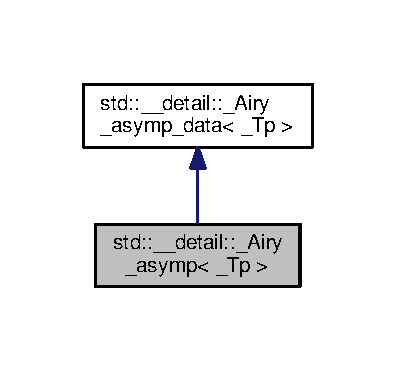
\includegraphics[width=190pt]{classstd_1_1____detail_1_1__Airy__asymp__inherit__graph}
\end{center}
\end{figure}


Collaboration diagram for std\+:\+:\+\_\+\+\_\+detail\+:\+:\+\_\+\+Airy\+\_\+asymp$<$ \+\_\+\+Tp $>$\+:
\nopagebreak
\begin{figure}[H]
\begin{center}
\leavevmode
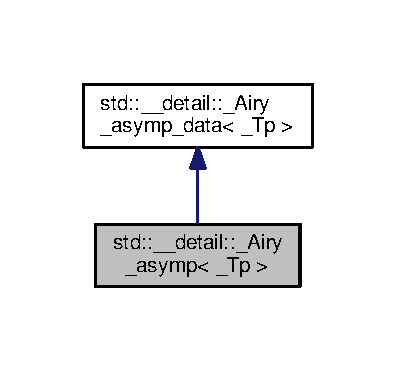
\includegraphics[width=190pt]{classstd_1_1____detail_1_1__Airy__asymp__coll__graph}
\end{center}
\end{figure}
\subsection*{Public Types}
\begin{DoxyCompactItemize}
\item 
using \hyperlink{classstd_1_1____detail_1_1__Airy__asymp_ae28f102423d34e78502ab6da42d67f50}{\+\_\+\+Cmplx} = std\+::complex$<$ \+\_\+\+Tp $>$
\end{DoxyCompactItemize}
\subsection*{Public Member Functions}
\begin{DoxyCompactItemize}
\item 
constexpr \hyperlink{classstd_1_1____detail_1_1__Airy__asymp_a93f2010a2c48be2f38445420ba019a52}{\+\_\+\+Airy\+\_\+asymp} ()=default
\item 
\hyperlink{structstd_1_1____detail_1_1__AiryState}{\+\_\+\+Airy\+State}$<$ \hyperlink{classstd_1_1____detail_1_1__Airy__asymp_ae28f102423d34e78502ab6da42d67f50}{\+\_\+\+Cmplx} $>$ \hyperlink{classstd_1_1____detail_1_1__Airy__asymp_ac3429a56fa955a3b8a71d450fd9662a6}{\+\_\+\+S\+\_\+absarg\+\_\+ge\+\_\+pio3} (\hyperlink{classstd_1_1____detail_1_1__Airy__asymp_ae28f102423d34e78502ab6da42d67f50}{\+\_\+\+Cmplx} \+\_\+\+\_\+z) const
\begin{DoxyCompactList}\small\item\em This function evaluates $ Ai(z), Ai'(z) $ and $ Bi(z), Bi'(z) $ from their asymptotic expansions for $ |arg(z)| < 2*\pi/3 $ i.\+e. roughly along the negative real axis. \end{DoxyCompactList}\item 
\hyperlink{structstd_1_1____detail_1_1__AiryState}{\+\_\+\+Airy\+State}$<$ \hyperlink{classstd_1_1____detail_1_1__Airy__asymp_ae28f102423d34e78502ab6da42d67f50}{\+\_\+\+Cmplx} $>$ \hyperlink{classstd_1_1____detail_1_1__Airy__asymp_a64bce3ed154b3268944ae20f324d64cd}{\+\_\+\+S\+\_\+absarg\+\_\+lt\+\_\+pio3} (\hyperlink{classstd_1_1____detail_1_1__Airy__asymp_ae28f102423d34e78502ab6da42d67f50}{\+\_\+\+Cmplx} \+\_\+\+\_\+z) const
\begin{DoxyCompactList}\small\item\em This function evaluates $ Ai(z) $ and $ Ai'(z) $ from their asymptotic expansions for $ |arg(-z)| < \pi/3 $ i.\+e. roughly along the negative real axis. \end{DoxyCompactList}\item 
\hyperlink{structstd_1_1____detail_1_1__AiryState}{\+\_\+\+Airy\+State}$<$ \hyperlink{classstd_1_1____detail_1_1__Airy__asymp_ae28f102423d34e78502ab6da42d67f50}{\+\_\+\+Cmplx} $>$ \hyperlink{classstd_1_1____detail_1_1__Airy__asymp_a79ba1c14d03fad8369477baf39c62874}{operator()} (\hyperlink{classstd_1_1____detail_1_1__Airy__asymp_ae28f102423d34e78502ab6da42d67f50}{\+\_\+\+Cmplx} \+\_\+\+\_\+t, bool \+\_\+\+\_\+return\+\_\+fock\+\_\+airy=false) const
\end{DoxyCompactItemize}


\subsection{Detailed Description}
\subsubsection*{template$<$typename \+\_\+\+Tp$>$\newline
class std\+::\+\_\+\+\_\+detail\+::\+\_\+\+Airy\+\_\+asymp$<$ \+\_\+\+Tp $>$}

A class encapsulating the asymptotic expansions of Airy functions and their derivatives.


\begin{DoxyTemplParams}{Template Parameters}
{\em \+\_\+\+Tp} & A real type \\
\hline
\end{DoxyTemplParams}


Definition at line 1997 of file sf\+\_\+airy.\+tcc.



\subsection{Member Typedef Documentation}
\mbox{\Hypertarget{classstd_1_1____detail_1_1__Airy__asymp_ae28f102423d34e78502ab6da42d67f50}\label{classstd_1_1____detail_1_1__Airy__asymp_ae28f102423d34e78502ab6da42d67f50}} 
\index{std\+::\+\_\+\+\_\+detail\+::\+\_\+\+Airy\+\_\+asymp@{std\+::\+\_\+\+\_\+detail\+::\+\_\+\+Airy\+\_\+asymp}!\+\_\+\+Cmplx@{\+\_\+\+Cmplx}}
\index{\+\_\+\+Cmplx@{\+\_\+\+Cmplx}!std\+::\+\_\+\+\_\+detail\+::\+\_\+\+Airy\+\_\+asymp@{std\+::\+\_\+\+\_\+detail\+::\+\_\+\+Airy\+\_\+asymp}}
\subsubsection{\texorpdfstring{\+\_\+\+Cmplx}{\_Cmplx}}
{\footnotesize\ttfamily template$<$typename \+\_\+\+Tp $>$ \\
using \hyperlink{classstd_1_1____detail_1_1__Airy__asymp}{std\+::\+\_\+\+\_\+detail\+::\+\_\+\+Airy\+\_\+asymp}$<$ \+\_\+\+Tp $>$\+::\hyperlink{classstd_1_1____detail_1_1__Airy__asymp_ae28f102423d34e78502ab6da42d67f50}{\+\_\+\+Cmplx} =  std\+::complex$<$\+\_\+\+Tp$>$}



Definition at line 2002 of file sf\+\_\+airy.\+tcc.



\subsection{Constructor \& Destructor Documentation}
\mbox{\Hypertarget{classstd_1_1____detail_1_1__Airy__asymp_a93f2010a2c48be2f38445420ba019a52}\label{classstd_1_1____detail_1_1__Airy__asymp_a93f2010a2c48be2f38445420ba019a52}} 
\index{std\+::\+\_\+\+\_\+detail\+::\+\_\+\+Airy\+\_\+asymp@{std\+::\+\_\+\+\_\+detail\+::\+\_\+\+Airy\+\_\+asymp}!\+\_\+\+Airy\+\_\+asymp@{\+\_\+\+Airy\+\_\+asymp}}
\index{\+\_\+\+Airy\+\_\+asymp@{\+\_\+\+Airy\+\_\+asymp}!std\+::\+\_\+\+\_\+detail\+::\+\_\+\+Airy\+\_\+asymp@{std\+::\+\_\+\+\_\+detail\+::\+\_\+\+Airy\+\_\+asymp}}
\subsubsection{\texorpdfstring{\+\_\+\+Airy\+\_\+asymp()}{\_Airy\_asymp()}}
{\footnotesize\ttfamily template$<$typename \+\_\+\+Tp $>$ \\
constexpr \hyperlink{classstd_1_1____detail_1_1__Airy__asymp}{std\+::\+\_\+\+\_\+detail\+::\+\_\+\+Airy\+\_\+asymp}$<$ \+\_\+\+Tp $>$\+::\hyperlink{classstd_1_1____detail_1_1__Airy__asymp}{\+\_\+\+Airy\+\_\+asymp} (\begin{DoxyParamCaption}{ }\end{DoxyParamCaption})\hspace{0.3cm}{\ttfamily [default]}}



\subsection{Member Function Documentation}
\mbox{\Hypertarget{classstd_1_1____detail_1_1__Airy__asymp_ac3429a56fa955a3b8a71d450fd9662a6}\label{classstd_1_1____detail_1_1__Airy__asymp_ac3429a56fa955a3b8a71d450fd9662a6}} 
\index{std\+::\+\_\+\+\_\+detail\+::\+\_\+\+Airy\+\_\+asymp@{std\+::\+\_\+\+\_\+detail\+::\+\_\+\+Airy\+\_\+asymp}!\+\_\+\+S\+\_\+absarg\+\_\+ge\+\_\+pio3@{\+\_\+\+S\+\_\+absarg\+\_\+ge\+\_\+pio3}}
\index{\+\_\+\+S\+\_\+absarg\+\_\+ge\+\_\+pio3@{\+\_\+\+S\+\_\+absarg\+\_\+ge\+\_\+pio3}!std\+::\+\_\+\+\_\+detail\+::\+\_\+\+Airy\+\_\+asymp@{std\+::\+\_\+\+\_\+detail\+::\+\_\+\+Airy\+\_\+asymp}}
\subsubsection{\texorpdfstring{\+\_\+\+S\+\_\+absarg\+\_\+ge\+\_\+pio3()}{\_S\_absarg\_ge\_pio3()}}
{\footnotesize\ttfamily template$<$typename \+\_\+\+Tp $>$ \\
\hyperlink{structstd_1_1____detail_1_1__AiryState}{\+\_\+\+Airy\+State}$<$ std\+::complex$<$ \+\_\+\+Tp $>$ $>$ \hyperlink{classstd_1_1____detail_1_1__Airy__asymp}{std\+::\+\_\+\+\_\+detail\+::\+\_\+\+Airy\+\_\+asymp}$<$ \+\_\+\+Tp $>$\+::\+\_\+\+S\+\_\+absarg\+\_\+ge\+\_\+pio3 (\begin{DoxyParamCaption}\item[{\hyperlink{classstd_1_1____detail_1_1__Airy__asymp_ae28f102423d34e78502ab6da42d67f50}{\+\_\+\+Cmplx}}]{\+\_\+\+\_\+z }\end{DoxyParamCaption}) const}



This function evaluates $ Ai(z), Ai'(z) $ and $ Bi(z), Bi'(z) $ from their asymptotic expansions for $ |arg(z)| < 2*\pi/3 $ i.\+e. roughly along the negative real axis. 


\begin{DoxyTemplParams}{Template Parameters}
{\em \+\_\+\+Tp} & A real type \\
\hline
\end{DoxyTemplParams}

\begin{DoxyParams}[1]{Parameters}
\mbox{\tt in}  & {\em \+\_\+\+\_\+z} & Complex argument at which Ai(z) and Bi(z) and their derivative are evaluated. This function assumes $ |z| > 15 $ and $ |(arg(z)| < 2\pi/3 $. \\
\hline
\end{DoxyParams}
\begin{DoxyReturn}{Returns}
A struct containing $ z, Ai(z), Ai'(z), Bi(z), Bi'(z) $. 
\end{DoxyReturn}


Definition at line 2270 of file sf\+\_\+airy.\+tcc.



References std\+::\+\_\+\+\_\+detail\+::\+\_\+\+Airy\+State$<$ \+\_\+\+Tp $>$\+::\+\_\+\+\_\+z.

\mbox{\Hypertarget{classstd_1_1____detail_1_1__Airy__asymp_a64bce3ed154b3268944ae20f324d64cd}\label{classstd_1_1____detail_1_1__Airy__asymp_a64bce3ed154b3268944ae20f324d64cd}} 
\index{std\+::\+\_\+\+\_\+detail\+::\+\_\+\+Airy\+\_\+asymp@{std\+::\+\_\+\+\_\+detail\+::\+\_\+\+Airy\+\_\+asymp}!\+\_\+\+S\+\_\+absarg\+\_\+lt\+\_\+pio3@{\+\_\+\+S\+\_\+absarg\+\_\+lt\+\_\+pio3}}
\index{\+\_\+\+S\+\_\+absarg\+\_\+lt\+\_\+pio3@{\+\_\+\+S\+\_\+absarg\+\_\+lt\+\_\+pio3}!std\+::\+\_\+\+\_\+detail\+::\+\_\+\+Airy\+\_\+asymp@{std\+::\+\_\+\+\_\+detail\+::\+\_\+\+Airy\+\_\+asymp}}
\subsubsection{\texorpdfstring{\+\_\+\+S\+\_\+absarg\+\_\+lt\+\_\+pio3()}{\_S\_absarg\_lt\_pio3()}}
{\footnotesize\ttfamily template$<$typename \+\_\+\+Tp $>$ \\
\hyperlink{structstd_1_1____detail_1_1__AiryState}{\+\_\+\+Airy\+State}$<$ std\+::complex$<$ \+\_\+\+Tp $>$ $>$ \hyperlink{classstd_1_1____detail_1_1__Airy__asymp}{std\+::\+\_\+\+\_\+detail\+::\+\_\+\+Airy\+\_\+asymp}$<$ \+\_\+\+Tp $>$\+::\+\_\+\+S\+\_\+absarg\+\_\+lt\+\_\+pio3 (\begin{DoxyParamCaption}\item[{\hyperlink{classstd_1_1____detail_1_1__Airy__asymp_ae28f102423d34e78502ab6da42d67f50}{\+\_\+\+Cmplx}}]{\+\_\+\+\_\+z }\end{DoxyParamCaption}) const}



This function evaluates $ Ai(z) $ and $ Ai'(z) $ from their asymptotic expansions for $ |arg(-z)| < \pi/3 $ i.\+e. roughly along the negative real axis. 

For speed, the number of terms needed to achieve about 16 decimals accuracy is tabled and determined for $ |z| $. This function assumes $ |z| > 15 $ and $ |arg(-z)| < \pi/3 $.

Note that for speed and since this function is called by another, checks for valid arguments are not made. Hence, an error return is not needed.


\begin{DoxyTemplParams}{Template Parameters}
{\em \+\_\+\+Tp} & A real type \\
\hline
\end{DoxyTemplParams}

\begin{DoxyParams}[1]{Parameters}
\mbox{\tt in}  & {\em \+\_\+\+\_\+z} & The value at which the Airy function and their derivatives are evaluated. \\
\hline
\end{DoxyParams}
\begin{DoxyReturn}{Returns}
A struct containing $ z, Ai(z), Ai'(z), Bi(z), Bi'(z) $. 
\end{DoxyReturn}
\begin{DoxyRefDesc}{Todo}
\item[\hyperlink{todo__todo000007}{Todo}]Revisit these numbers of terms for the Airy asymptotic expansions. \end{DoxyRefDesc}


Definition at line 2300 of file sf\+\_\+airy.\+tcc.



References std\+::\+\_\+\+\_\+detail\+::\+\_\+\+Airy\+State$<$ \+\_\+\+Tp $>$\+::\+\_\+\+\_\+z.

\mbox{\Hypertarget{classstd_1_1____detail_1_1__Airy__asymp_a79ba1c14d03fad8369477baf39c62874}\label{classstd_1_1____detail_1_1__Airy__asymp_a79ba1c14d03fad8369477baf39c62874}} 
\index{std\+::\+\_\+\+\_\+detail\+::\+\_\+\+Airy\+\_\+asymp@{std\+::\+\_\+\+\_\+detail\+::\+\_\+\+Airy\+\_\+asymp}!operator()@{operator()}}
\index{operator()@{operator()}!std\+::\+\_\+\+\_\+detail\+::\+\_\+\+Airy\+\_\+asymp@{std\+::\+\_\+\+\_\+detail\+::\+\_\+\+Airy\+\_\+asymp}}
\subsubsection{\texorpdfstring{operator()()}{operator()()}}
{\footnotesize\ttfamily template$<$typename \+\_\+\+Tp $>$ \\
\hyperlink{structstd_1_1____detail_1_1__AiryState}{\+\_\+\+Airy\+State}$<$ std\+::complex$<$ \+\_\+\+Tp $>$ $>$ \hyperlink{classstd_1_1____detail_1_1__Airy__asymp}{std\+::\+\_\+\+\_\+detail\+::\+\_\+\+Airy\+\_\+asymp}$<$ \+\_\+\+Tp $>$\+::operator() (\begin{DoxyParamCaption}\item[{\hyperlink{classstd_1_1____detail_1_1__Airy__asymp_ae28f102423d34e78502ab6da42d67f50}{\+\_\+\+Cmplx}}]{\+\_\+\+\_\+t,  }\item[{bool}]{\+\_\+\+\_\+return\+\_\+fock\+\_\+airy = {\ttfamily false} }\end{DoxyParamCaption}) const}

Return the Airy functions for a given argument using asymptotic series.


\begin{DoxyTemplParams}{Template Parameters}
{\em \+\_\+\+Tp} & A real type \\
\hline
\end{DoxyTemplParams}


Definition at line 2028 of file sf\+\_\+airy.\+tcc.



References std\+::\+\_\+\+\_\+detail\+::\+\_\+\+Airy\+State$<$ \+\_\+\+Tp $>$\+::\+\_\+\+\_\+z.



The documentation for this class was generated from the following file\+:\begin{DoxyCompactItemize}
\item 
include/bits/\hyperlink{sf__airy_8tcc}{sf\+\_\+airy.\+tcc}\end{DoxyCompactItemize}

\hypertarget{structstd_1_1____detail_1_1__Airy__asymp__data}{}\section{std\+:\+:\+\_\+\+\_\+detail\+:\+:\+\_\+\+Airy\+\_\+asymp\+\_\+data$<$ \+\_\+\+Tp $>$ Struct Template Reference}
\label{structstd_1_1____detail_1_1__Airy__asymp__data}\index{std\+::\+\_\+\+\_\+detail\+::\+\_\+\+Airy\+\_\+asymp\+\_\+data$<$ \+\_\+\+Tp $>$@{std\+::\+\_\+\+\_\+detail\+::\+\_\+\+Airy\+\_\+asymp\+\_\+data$<$ \+\_\+\+Tp $>$}}


Inheritance diagram for std\+:\+:\+\_\+\+\_\+detail\+:\+:\+\_\+\+Airy\+\_\+asymp\+\_\+data$<$ \+\_\+\+Tp $>$\+:
\nopagebreak
\begin{figure}[H]
\begin{center}
\leavevmode
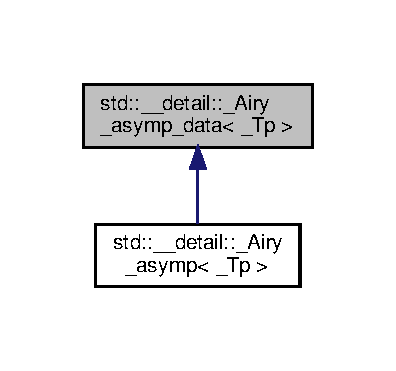
\includegraphics[width=190pt]{structstd_1_1____detail_1_1__Airy__asymp__data__inherit__graph}
\end{center}
\end{figure}


\subsection{Detailed Description}
\subsubsection*{template$<$typename \+\_\+\+Tp$>$\newline
struct std\+::\+\_\+\+\_\+detail\+::\+\_\+\+Airy\+\_\+asymp\+\_\+data$<$ \+\_\+\+Tp $>$}

A class encapsulating data for the asymptotic expansions of Airy functions and their derivatives.


\begin{DoxyTemplParams}{Template Parameters}
{\em \+\_\+\+Tp} & A real type \\
\hline
\end{DoxyTemplParams}


Definition at line 632 of file sf\+\_\+airy.\+tcc.



The documentation for this struct was generated from the following file\+:\begin{DoxyCompactItemize}
\item 
bits/\hyperlink{sf__airy_8tcc}{sf\+\_\+airy.\+tcc}\end{DoxyCompactItemize}

\hypertarget{structstd_1_1____detail_1_1__Airy__asymp__data_3_01double_01_4}{}\section{std\+:\+:\+\_\+\+\_\+detail\+:\+:\+\_\+\+Airy\+\_\+asymp\+\_\+data$<$ double $>$ Struct Template Reference}
\label{structstd_1_1____detail_1_1__Airy__asymp__data_3_01double_01_4}\index{std\+::\+\_\+\+\_\+detail\+::\+\_\+\+Airy\+\_\+asymp\+\_\+data$<$ double $>$@{std\+::\+\_\+\+\_\+detail\+::\+\_\+\+Airy\+\_\+asymp\+\_\+data$<$ double $>$}}
\subsection*{Static Public Attributes}
\begin{DoxyCompactItemize}
\item 
static constexpr double \hyperlink{structstd_1_1____detail_1_1__Airy__asymp__data_3_01double_01_4_a38e855b175c89166c4220cacd07ca1c7}{\+\_\+\+S\+\_\+c} \mbox{[}\hyperlink{structstd_1_1____detail_1_1__Airy__asymp__data_3_01double_01_4_a38e485184d2762e83a27937efc343d01}{\+\_\+\+S\+\_\+max\+\_\+cd}\mbox{]}
\item 
static constexpr double \hyperlink{structstd_1_1____detail_1_1__Airy__asymp__data_3_01double_01_4_aeaf6aab79b67a46932e9d16864ad0f78}{\+\_\+\+S\+\_\+d} \mbox{[}\hyperlink{structstd_1_1____detail_1_1__Airy__asymp__data_3_01double_01_4_a38e485184d2762e83a27937efc343d01}{\+\_\+\+S\+\_\+max\+\_\+cd}\mbox{]}
\item 
static constexpr int \hyperlink{structstd_1_1____detail_1_1__Airy__asymp__data_3_01double_01_4_a38e485184d2762e83a27937efc343d01}{\+\_\+\+S\+\_\+max\+\_\+cd} = 198
\end{DoxyCompactItemize}


\subsection{Detailed Description}
\subsubsection*{template$<$$>$\newline
struct std\+::\+\_\+\+\_\+detail\+::\+\_\+\+Airy\+\_\+asymp\+\_\+data$<$ double $>$}



Definition at line 738 of file sf\+\_\+airy.\+tcc.



\subsection{Member Data Documentation}
\mbox{\Hypertarget{structstd_1_1____detail_1_1__Airy__asymp__data_3_01double_01_4_a38e855b175c89166c4220cacd07ca1c7}\label{structstd_1_1____detail_1_1__Airy__asymp__data_3_01double_01_4_a38e855b175c89166c4220cacd07ca1c7}} 
\index{std\+::\+\_\+\+\_\+detail\+::\+\_\+\+Airy\+\_\+asymp\+\_\+data$<$ double $>$@{std\+::\+\_\+\+\_\+detail\+::\+\_\+\+Airy\+\_\+asymp\+\_\+data$<$ double $>$}!\+\_\+\+S\+\_\+c@{\+\_\+\+S\+\_\+c}}
\index{\+\_\+\+S\+\_\+c@{\+\_\+\+S\+\_\+c}!std\+::\+\_\+\+\_\+detail\+::\+\_\+\+Airy\+\_\+asymp\+\_\+data$<$ double $>$@{std\+::\+\_\+\+\_\+detail\+::\+\_\+\+Airy\+\_\+asymp\+\_\+data$<$ double $>$}}
\subsubsection{\texorpdfstring{\+\_\+\+S\+\_\+c}{\_S\_c}}
{\footnotesize\ttfamily constexpr double \hyperlink{structstd_1_1____detail_1_1__Airy__asymp__data}{std\+::\+\_\+\+\_\+detail\+::\+\_\+\+Airy\+\_\+asymp\+\_\+data}$<$ double $>$\+::\+\_\+\+S\+\_\+c\mbox{[}\hyperlink{structstd_1_1____detail_1_1__Airy__asymp__data_3_01double_01_4_a38e485184d2762e83a27937efc343d01}{\+\_\+\+S\+\_\+max\+\_\+cd}\mbox{]}\hspace{0.3cm}{\ttfamily [static]}}



Definition at line 744 of file sf\+\_\+airy.\+tcc.

\mbox{\Hypertarget{structstd_1_1____detail_1_1__Airy__asymp__data_3_01double_01_4_aeaf6aab79b67a46932e9d16864ad0f78}\label{structstd_1_1____detail_1_1__Airy__asymp__data_3_01double_01_4_aeaf6aab79b67a46932e9d16864ad0f78}} 
\index{std\+::\+\_\+\+\_\+detail\+::\+\_\+\+Airy\+\_\+asymp\+\_\+data$<$ double $>$@{std\+::\+\_\+\+\_\+detail\+::\+\_\+\+Airy\+\_\+asymp\+\_\+data$<$ double $>$}!\+\_\+\+S\+\_\+d@{\+\_\+\+S\+\_\+d}}
\index{\+\_\+\+S\+\_\+d@{\+\_\+\+S\+\_\+d}!std\+::\+\_\+\+\_\+detail\+::\+\_\+\+Airy\+\_\+asymp\+\_\+data$<$ double $>$@{std\+::\+\_\+\+\_\+detail\+::\+\_\+\+Airy\+\_\+asymp\+\_\+data$<$ double $>$}}
\subsubsection{\texorpdfstring{\+\_\+\+S\+\_\+d}{\_S\_d}}
{\footnotesize\ttfamily constexpr double \hyperlink{structstd_1_1____detail_1_1__Airy__asymp__data}{std\+::\+\_\+\+\_\+detail\+::\+\_\+\+Airy\+\_\+asymp\+\_\+data}$<$ double $>$\+::\+\_\+\+S\+\_\+d\mbox{[}\hyperlink{structstd_1_1____detail_1_1__Airy__asymp__data_3_01double_01_4_a38e485184d2762e83a27937efc343d01}{\+\_\+\+S\+\_\+max\+\_\+cd}\mbox{]}\hspace{0.3cm}{\ttfamily [static]}}



Definition at line 947 of file sf\+\_\+airy.\+tcc.

\mbox{\Hypertarget{structstd_1_1____detail_1_1__Airy__asymp__data_3_01double_01_4_a38e485184d2762e83a27937efc343d01}\label{structstd_1_1____detail_1_1__Airy__asymp__data_3_01double_01_4_a38e485184d2762e83a27937efc343d01}} 
\index{std\+::\+\_\+\+\_\+detail\+::\+\_\+\+Airy\+\_\+asymp\+\_\+data$<$ double $>$@{std\+::\+\_\+\+\_\+detail\+::\+\_\+\+Airy\+\_\+asymp\+\_\+data$<$ double $>$}!\+\_\+\+S\+\_\+max\+\_\+cd@{\+\_\+\+S\+\_\+max\+\_\+cd}}
\index{\+\_\+\+S\+\_\+max\+\_\+cd@{\+\_\+\+S\+\_\+max\+\_\+cd}!std\+::\+\_\+\+\_\+detail\+::\+\_\+\+Airy\+\_\+asymp\+\_\+data$<$ double $>$@{std\+::\+\_\+\+\_\+detail\+::\+\_\+\+Airy\+\_\+asymp\+\_\+data$<$ double $>$}}
\subsubsection{\texorpdfstring{\+\_\+\+S\+\_\+max\+\_\+cd}{\_S\_max\_cd}}
{\footnotesize\ttfamily constexpr int \hyperlink{structstd_1_1____detail_1_1__Airy__asymp__data}{std\+::\+\_\+\+\_\+detail\+::\+\_\+\+Airy\+\_\+asymp\+\_\+data}$<$ double $>$\+::\+\_\+\+S\+\_\+max\+\_\+cd = 198\hspace{0.3cm}{\ttfamily [static]}}



Definition at line 740 of file sf\+\_\+airy.\+tcc.



The documentation for this struct was generated from the following file\+:\begin{DoxyCompactItemize}
\item 
bits/\hyperlink{sf__airy_8tcc}{sf\+\_\+airy.\+tcc}\end{DoxyCompactItemize}

\hypertarget{structstd_1_1____detail_1_1__Airy__asymp__data_3_01float_01_4}{}\section{std\+:\+:\+\_\+\+\_\+detail\+:\+:\+\_\+\+Airy\+\_\+asymp\+\_\+data$<$ float $>$ Struct Template Reference}
\label{structstd_1_1____detail_1_1__Airy__asymp__data_3_01float_01_4}\index{std\+::\+\_\+\+\_\+detail\+::\+\_\+\+Airy\+\_\+asymp\+\_\+data$<$ float $>$@{std\+::\+\_\+\+\_\+detail\+::\+\_\+\+Airy\+\_\+asymp\+\_\+data$<$ float $>$}}
\subsection*{Static Public Attributes}
\begin{DoxyCompactItemize}
\item 
static constexpr float \hyperlink{structstd_1_1____detail_1_1__Airy__asymp__data_3_01float_01_4_a8fc68acdbcbc59f4ecfdd4bc2f4f2a1e}{\+\_\+\+S\+\_\+c} \mbox{[}\hyperlink{structstd_1_1____detail_1_1__Airy__asymp__data_3_01float_01_4_ac0e59b83a90623587f20cdc32a9e7565}{\+\_\+\+S\+\_\+max\+\_\+cd}\mbox{]}
\item 
static constexpr float \hyperlink{structstd_1_1____detail_1_1__Airy__asymp__data_3_01float_01_4_ad947443d5860fcd25d25ad6d04ea3bb3}{\+\_\+\+S\+\_\+d} \mbox{[}\hyperlink{structstd_1_1____detail_1_1__Airy__asymp__data_3_01float_01_4_ac0e59b83a90623587f20cdc32a9e7565}{\+\_\+\+S\+\_\+max\+\_\+cd}\mbox{]}
\item 
static constexpr int \hyperlink{structstd_1_1____detail_1_1__Airy__asymp__data_3_01float_01_4_ac0e59b83a90623587f20cdc32a9e7565}{\+\_\+\+S\+\_\+max\+\_\+cd} = 43
\end{DoxyCompactItemize}


\subsection{Detailed Description}
\subsubsection*{template$<$$>$\\*
struct std\+::\+\_\+\+\_\+detail\+::\+\_\+\+Airy\+\_\+asymp\+\_\+data$<$ float $>$}



Definition at line 636 of file sf\+\_\+airy.\+tcc.



\subsection{Member Data Documentation}
\index{std\+::\+\_\+\+\_\+detail\+::\+\_\+\+Airy\+\_\+asymp\+\_\+data$<$ float $>$@{std\+::\+\_\+\+\_\+detail\+::\+\_\+\+Airy\+\_\+asymp\+\_\+data$<$ float $>$}!\+\_\+\+S\+\_\+c@{\+\_\+\+S\+\_\+c}}
\index{\+\_\+\+S\+\_\+c@{\+\_\+\+S\+\_\+c}!std\+::\+\_\+\+\_\+detail\+::\+\_\+\+Airy\+\_\+asymp\+\_\+data$<$ float $>$@{std\+::\+\_\+\+\_\+detail\+::\+\_\+\+Airy\+\_\+asymp\+\_\+data$<$ float $>$}}
\subsubsection[{\texorpdfstring{\+\_\+\+S\+\_\+c}{_S_c}}]{\setlength{\rightskip}{0pt plus 5cm}constexpr float {\bf std\+::\+\_\+\+\_\+detail\+::\+\_\+\+Airy\+\_\+asymp\+\_\+data}$<$ float $>$\+::\+\_\+\+S\+\_\+c\mbox{[}{\bf \+\_\+\+S\+\_\+max\+\_\+cd}\mbox{]}\hspace{0.3cm}{\ttfamily [static]}}\hypertarget{structstd_1_1____detail_1_1__Airy__asymp__data_3_01float_01_4_a8fc68acdbcbc59f4ecfdd4bc2f4f2a1e}{}\label{structstd_1_1____detail_1_1__Airy__asymp__data_3_01float_01_4_a8fc68acdbcbc59f4ecfdd4bc2f4f2a1e}


Definition at line 642 of file sf\+\_\+airy.\+tcc.

\index{std\+::\+\_\+\+\_\+detail\+::\+\_\+\+Airy\+\_\+asymp\+\_\+data$<$ float $>$@{std\+::\+\_\+\+\_\+detail\+::\+\_\+\+Airy\+\_\+asymp\+\_\+data$<$ float $>$}!\+\_\+\+S\+\_\+d@{\+\_\+\+S\+\_\+d}}
\index{\+\_\+\+S\+\_\+d@{\+\_\+\+S\+\_\+d}!std\+::\+\_\+\+\_\+detail\+::\+\_\+\+Airy\+\_\+asymp\+\_\+data$<$ float $>$@{std\+::\+\_\+\+\_\+detail\+::\+\_\+\+Airy\+\_\+asymp\+\_\+data$<$ float $>$}}
\subsubsection[{\texorpdfstring{\+\_\+\+S\+\_\+d}{_S_d}}]{\setlength{\rightskip}{0pt plus 5cm}constexpr float {\bf std\+::\+\_\+\+\_\+detail\+::\+\_\+\+Airy\+\_\+asymp\+\_\+data}$<$ float $>$\+::\+\_\+\+S\+\_\+d\mbox{[}{\bf \+\_\+\+S\+\_\+max\+\_\+cd}\mbox{]}\hspace{0.3cm}{\ttfamily [static]}}\hypertarget{structstd_1_1____detail_1_1__Airy__asymp__data_3_01float_01_4_ad947443d5860fcd25d25ad6d04ea3bb3}{}\label{structstd_1_1____detail_1_1__Airy__asymp__data_3_01float_01_4_ad947443d5860fcd25d25ad6d04ea3bb3}


Definition at line 690 of file sf\+\_\+airy.\+tcc.

\index{std\+::\+\_\+\+\_\+detail\+::\+\_\+\+Airy\+\_\+asymp\+\_\+data$<$ float $>$@{std\+::\+\_\+\+\_\+detail\+::\+\_\+\+Airy\+\_\+asymp\+\_\+data$<$ float $>$}!\+\_\+\+S\+\_\+max\+\_\+cd@{\+\_\+\+S\+\_\+max\+\_\+cd}}
\index{\+\_\+\+S\+\_\+max\+\_\+cd@{\+\_\+\+S\+\_\+max\+\_\+cd}!std\+::\+\_\+\+\_\+detail\+::\+\_\+\+Airy\+\_\+asymp\+\_\+data$<$ float $>$@{std\+::\+\_\+\+\_\+detail\+::\+\_\+\+Airy\+\_\+asymp\+\_\+data$<$ float $>$}}
\subsubsection[{\texorpdfstring{\+\_\+\+S\+\_\+max\+\_\+cd}{_S_max_cd}}]{\setlength{\rightskip}{0pt plus 5cm}constexpr int {\bf std\+::\+\_\+\+\_\+detail\+::\+\_\+\+Airy\+\_\+asymp\+\_\+data}$<$ float $>$\+::\+\_\+\+S\+\_\+max\+\_\+cd = 43\hspace{0.3cm}{\ttfamily [static]}}\hypertarget{structstd_1_1____detail_1_1__Airy__asymp__data_3_01float_01_4_ac0e59b83a90623587f20cdc32a9e7565}{}\label{structstd_1_1____detail_1_1__Airy__asymp__data_3_01float_01_4_ac0e59b83a90623587f20cdc32a9e7565}


Definition at line 638 of file sf\+\_\+airy.\+tcc.



The documentation for this struct was generated from the following file\+:\begin{DoxyCompactItemize}
\item 
bits/\hyperlink{sf__airy_8tcc}{sf\+\_\+airy.\+tcc}\end{DoxyCompactItemize}

\hypertarget{structstd_1_1____detail_1_1__Airy__asymp__data_3_01long_01double_01_4}{}\section{std\+:\+:\+\_\+\+\_\+detail\+:\+:\+\_\+\+Airy\+\_\+asymp\+\_\+data$<$ long double $>$ Struct Template Reference}
\label{structstd_1_1____detail_1_1__Airy__asymp__data_3_01long_01double_01_4}\index{std\+::\+\_\+\+\_\+detail\+::\+\_\+\+Airy\+\_\+asymp\+\_\+data$<$ long double $>$@{std\+::\+\_\+\+\_\+detail\+::\+\_\+\+Airy\+\_\+asymp\+\_\+data$<$ long double $>$}}
\subsection*{Static Public Attributes}
\begin{DoxyCompactItemize}
\item 
static constexpr long double \hyperlink{structstd_1_1____detail_1_1__Airy__asymp__data_3_01long_01double_01_4_a563bbe7d1ef612defb41aaedcc5657fe}{\+\_\+\+S\+\_\+c} \mbox{[}\hyperlink{structstd_1_1____detail_1_1__Airy__asymp__data_3_01long_01double_01_4_a6a21ac69ffc53d33ebc346981bc52b9a}{\+\_\+\+S\+\_\+max\+\_\+cd}\mbox{]}
\item 
static constexpr long double \hyperlink{structstd_1_1____detail_1_1__Airy__asymp__data_3_01long_01double_01_4_a3c49ca222e675f3def5077e46c7d6834}{\+\_\+\+S\+\_\+d} \mbox{[}\hyperlink{structstd_1_1____detail_1_1__Airy__asymp__data_3_01long_01double_01_4_a6a21ac69ffc53d33ebc346981bc52b9a}{\+\_\+\+S\+\_\+max\+\_\+cd}\mbox{]}
\item 
static constexpr int \hyperlink{structstd_1_1____detail_1_1__Airy__asymp__data_3_01long_01double_01_4_a6a21ac69ffc53d33ebc346981bc52b9a}{\+\_\+\+S\+\_\+max\+\_\+cd} = 201
\end{DoxyCompactItemize}


\subsection{Detailed Description}
\subsubsection*{template$<$$>$\\*
struct std\+::\+\_\+\+\_\+detail\+::\+\_\+\+Airy\+\_\+asymp\+\_\+data$<$ long double $>$}



Definition at line 2387 of file sf\+\_\+airy.\+tcc.



\subsection{Member Data Documentation}
\index{std\+::\+\_\+\+\_\+detail\+::\+\_\+\+Airy\+\_\+asymp\+\_\+data$<$ long double $>$@{std\+::\+\_\+\+\_\+detail\+::\+\_\+\+Airy\+\_\+asymp\+\_\+data$<$ long double $>$}!\+\_\+\+S\+\_\+c@{\+\_\+\+S\+\_\+c}}
\index{\+\_\+\+S\+\_\+c@{\+\_\+\+S\+\_\+c}!std\+::\+\_\+\+\_\+detail\+::\+\_\+\+Airy\+\_\+asymp\+\_\+data$<$ long double $>$@{std\+::\+\_\+\+\_\+detail\+::\+\_\+\+Airy\+\_\+asymp\+\_\+data$<$ long double $>$}}
\subsubsection[{\texorpdfstring{\+\_\+\+S\+\_\+c}{_S_c}}]{\setlength{\rightskip}{0pt plus 5cm}constexpr long double {\bf std\+::\+\_\+\+\_\+detail\+::\+\_\+\+Airy\+\_\+asymp\+\_\+data}$<$ long double $>$\+::\+\_\+\+S\+\_\+c\mbox{[}{\bf \+\_\+\+S\+\_\+max\+\_\+cd}\mbox{]}\hspace{0.3cm}{\ttfamily [static]}}\hypertarget{structstd_1_1____detail_1_1__Airy__asymp__data_3_01long_01double_01_4_a563bbe7d1ef612defb41aaedcc5657fe}{}\label{structstd_1_1____detail_1_1__Airy__asymp__data_3_01long_01double_01_4_a563bbe7d1ef612defb41aaedcc5657fe}


Definition at line 2393 of file sf\+\_\+airy.\+tcc.

\index{std\+::\+\_\+\+\_\+detail\+::\+\_\+\+Airy\+\_\+asymp\+\_\+data$<$ long double $>$@{std\+::\+\_\+\+\_\+detail\+::\+\_\+\+Airy\+\_\+asymp\+\_\+data$<$ long double $>$}!\+\_\+\+S\+\_\+d@{\+\_\+\+S\+\_\+d}}
\index{\+\_\+\+S\+\_\+d@{\+\_\+\+S\+\_\+d}!std\+::\+\_\+\+\_\+detail\+::\+\_\+\+Airy\+\_\+asymp\+\_\+data$<$ long double $>$@{std\+::\+\_\+\+\_\+detail\+::\+\_\+\+Airy\+\_\+asymp\+\_\+data$<$ long double $>$}}
\subsubsection[{\texorpdfstring{\+\_\+\+S\+\_\+d}{_S_d}}]{\setlength{\rightskip}{0pt plus 5cm}constexpr long double {\bf std\+::\+\_\+\+\_\+detail\+::\+\_\+\+Airy\+\_\+asymp\+\_\+data}$<$ long double $>$\+::\+\_\+\+S\+\_\+d\mbox{[}{\bf \+\_\+\+S\+\_\+max\+\_\+cd}\mbox{]}\hspace{0.3cm}{\ttfamily [static]}}\hypertarget{structstd_1_1____detail_1_1__Airy__asymp__data_3_01long_01double_01_4_a3c49ca222e675f3def5077e46c7d6834}{}\label{structstd_1_1____detail_1_1__Airy__asymp__data_3_01long_01double_01_4_a3c49ca222e675f3def5077e46c7d6834}


Definition at line 2599 of file sf\+\_\+airy.\+tcc.

\index{std\+::\+\_\+\+\_\+detail\+::\+\_\+\+Airy\+\_\+asymp\+\_\+data$<$ long double $>$@{std\+::\+\_\+\+\_\+detail\+::\+\_\+\+Airy\+\_\+asymp\+\_\+data$<$ long double $>$}!\+\_\+\+S\+\_\+max\+\_\+cd@{\+\_\+\+S\+\_\+max\+\_\+cd}}
\index{\+\_\+\+S\+\_\+max\+\_\+cd@{\+\_\+\+S\+\_\+max\+\_\+cd}!std\+::\+\_\+\+\_\+detail\+::\+\_\+\+Airy\+\_\+asymp\+\_\+data$<$ long double $>$@{std\+::\+\_\+\+\_\+detail\+::\+\_\+\+Airy\+\_\+asymp\+\_\+data$<$ long double $>$}}
\subsubsection[{\texorpdfstring{\+\_\+\+S\+\_\+max\+\_\+cd}{_S_max_cd}}]{\setlength{\rightskip}{0pt plus 5cm}constexpr int {\bf std\+::\+\_\+\+\_\+detail\+::\+\_\+\+Airy\+\_\+asymp\+\_\+data}$<$ long double $>$\+::\+\_\+\+S\+\_\+max\+\_\+cd = 201\hspace{0.3cm}{\ttfamily [static]}}\hypertarget{structstd_1_1____detail_1_1__Airy__asymp__data_3_01long_01double_01_4_a6a21ac69ffc53d33ebc346981bc52b9a}{}\label{structstd_1_1____detail_1_1__Airy__asymp__data_3_01long_01double_01_4_a6a21ac69ffc53d33ebc346981bc52b9a}


Definition at line 2389 of file sf\+\_\+airy.\+tcc.



The documentation for this struct was generated from the following file\+:\begin{DoxyCompactItemize}
\item 
bits/\hyperlink{sf__airy_8tcc}{sf\+\_\+airy.\+tcc}\end{DoxyCompactItemize}

\hypertarget{classstd_1_1____detail_1_1__Airy__asymp__series}{}\section{std\+:\+:\+\_\+\+\_\+detail\+:\+:\+\_\+\+Airy\+\_\+asymp\+\_\+series$<$ \+\_\+\+Sum $>$ Class Template Reference}
\label{classstd_1_1____detail_1_1__Airy__asymp__series}\index{std\+::\+\_\+\+\_\+detail\+::\+\_\+\+Airy\+\_\+asymp\+\_\+series$<$ \+\_\+\+Sum $>$@{std\+::\+\_\+\+\_\+detail\+::\+\_\+\+Airy\+\_\+asymp\+\_\+series$<$ \+\_\+\+Sum $>$}}
\subsection*{Public Types}
\begin{DoxyCompactItemize}
\item 
using \hyperlink{classstd_1_1____detail_1_1__Airy__asymp__series_a17ec74b13ebc38d5531bf27cd31684fb}{scalar\+\_\+type} = std\+::\+\_\+\+\_\+detail\+::\+\_\+\+\_\+num\+\_\+traits\+\_\+t$<$ \hyperlink{classstd_1_1____detail_1_1__Airy__asymp__series_a729a698f23629a2f94b6ef71f377efc5}{value\+\_\+type} $>$
\item 
using \hyperlink{classstd_1_1____detail_1_1__Airy__asymp__series_a729a698f23629a2f94b6ef71f377efc5}{value\+\_\+type} = typename \+\_\+\+Sum\+::value\+\_\+type
\end{DoxyCompactItemize}
\subsection*{Public Member Functions}
\begin{DoxyCompactItemize}
\item 
\hyperlink{classstd_1_1____detail_1_1__Airy__asymp__series_a2768b3e101876b969b606cbde8b2e133}{\+\_\+\+Airy\+\_\+asymp\+\_\+series} (\+\_\+\+Sum \+\_\+\+\_\+proto)
\item 
\hyperlink{classstd_1_1____detail_1_1__Airy__asymp__series_a48eab98c05f50ad5b5f00f1ad9628e14}{\+\_\+\+Airy\+\_\+asymp\+\_\+series} (const \hyperlink{classstd_1_1____detail_1_1__Airy__asymp__series}{\+\_\+\+Airy\+\_\+asymp\+\_\+series} \&)=default
\item 
\hyperlink{classstd_1_1____detail_1_1__Airy__asymp__series_a967f89ea4dfc21c982fdc61315ea720d}{\+\_\+\+Airy\+\_\+asymp\+\_\+series} (\hyperlink{classstd_1_1____detail_1_1__Airy__asymp__series}{\+\_\+\+Airy\+\_\+asymp\+\_\+series} \&\&)=default
\item 
\hyperlink{structstd_1_1____detail_1_1__AiryState}{\+\_\+\+Airy\+State}$<$ \hyperlink{classstd_1_1____detail_1_1__Airy__asymp__series_a729a698f23629a2f94b6ef71f377efc5}{value\+\_\+type} $>$ \hyperlink{classstd_1_1____detail_1_1__Airy__asymp__series_acd5ce4d332334a4f669a981d588b417c}{operator()} (\hyperlink{classstd_1_1____detail_1_1__Airy__asymp__series_a729a698f23629a2f94b6ef71f377efc5}{value\+\_\+type} \+\_\+\+\_\+y)
\end{DoxyCompactItemize}
\subsection*{Static Public Attributes}
\begin{DoxyCompactItemize}
\item 
static constexpr \hyperlink{classstd_1_1____detail_1_1__Airy__asymp__series_a17ec74b13ebc38d5531bf27cd31684fb}{scalar\+\_\+type} \hyperlink{classstd_1_1____detail_1_1__Airy__asymp__series_a0a4d017f86429e22f5939e689e7b93ca}{\+\_\+\+S\+\_\+sqrt\+\_\+pi} = \+\_\+\+\_\+gnu\+\_\+cxx\+::\+\_\+\+\_\+const\+\_\+root\+\_\+pi(\hyperlink{classstd_1_1____detail_1_1__Airy__asymp__series_a17ec74b13ebc38d5531bf27cd31684fb}{scalar\+\_\+type}\{\})
\end{DoxyCompactItemize}


\subsection{Detailed Description}
\subsubsection*{template$<$typename \+\_\+\+Sum$>$\\*
class std\+::\+\_\+\+\_\+detail\+::\+\_\+\+Airy\+\_\+asymp\+\_\+series$<$ \+\_\+\+Sum $>$}

Class to manage the asymptotic series for Airy functions.


\begin{DoxyTemplParams}{Template Parameters}
{\em \+\_\+\+Sum} & A sum type \\
\hline
\end{DoxyTemplParams}


Definition at line 2364 of file sf\+\_\+airy.\+tcc.



\subsection{Member Typedef Documentation}
\index{std\+::\+\_\+\+\_\+detail\+::\+\_\+\+Airy\+\_\+asymp\+\_\+series@{std\+::\+\_\+\+\_\+detail\+::\+\_\+\+Airy\+\_\+asymp\+\_\+series}!scalar\+\_\+type@{scalar\+\_\+type}}
\index{scalar\+\_\+type@{scalar\+\_\+type}!std\+::\+\_\+\+\_\+detail\+::\+\_\+\+Airy\+\_\+asymp\+\_\+series@{std\+::\+\_\+\+\_\+detail\+::\+\_\+\+Airy\+\_\+asymp\+\_\+series}}
\subsubsection[{\texorpdfstring{scalar\+\_\+type}{scalar_type}}]{\setlength{\rightskip}{0pt plus 5cm}template$<$typename \+\_\+\+Sum$>$ using {\bf std\+::\+\_\+\+\_\+detail\+::\+\_\+\+Airy\+\_\+asymp\+\_\+series}$<$ \+\_\+\+Sum $>$\+::{\bf scalar\+\_\+type} =  std\+::\+\_\+\+\_\+detail\+::\+\_\+\+\_\+num\+\_\+traits\+\_\+t$<${\bf value\+\_\+type}$>$}\hypertarget{classstd_1_1____detail_1_1__Airy__asymp__series_a17ec74b13ebc38d5531bf27cd31684fb}{}\label{classstd_1_1____detail_1_1__Airy__asymp__series_a17ec74b13ebc38d5531bf27cd31684fb}


Definition at line 2369 of file sf\+\_\+airy.\+tcc.

\index{std\+::\+\_\+\+\_\+detail\+::\+\_\+\+Airy\+\_\+asymp\+\_\+series@{std\+::\+\_\+\+\_\+detail\+::\+\_\+\+Airy\+\_\+asymp\+\_\+series}!value\+\_\+type@{value\+\_\+type}}
\index{value\+\_\+type@{value\+\_\+type}!std\+::\+\_\+\+\_\+detail\+::\+\_\+\+Airy\+\_\+asymp\+\_\+series@{std\+::\+\_\+\+\_\+detail\+::\+\_\+\+Airy\+\_\+asymp\+\_\+series}}
\subsubsection[{\texorpdfstring{value\+\_\+type}{value_type}}]{\setlength{\rightskip}{0pt plus 5cm}template$<$typename \+\_\+\+Sum$>$ using {\bf std\+::\+\_\+\+\_\+detail\+::\+\_\+\+Airy\+\_\+asymp\+\_\+series}$<$ \+\_\+\+Sum $>$\+::{\bf value\+\_\+type} =  typename \+\_\+\+Sum\+::value\+\_\+type}\hypertarget{classstd_1_1____detail_1_1__Airy__asymp__series_a729a698f23629a2f94b6ef71f377efc5}{}\label{classstd_1_1____detail_1_1__Airy__asymp__series_a729a698f23629a2f94b6ef71f377efc5}


Definition at line 2368 of file sf\+\_\+airy.\+tcc.



\subsection{Constructor \& Destructor Documentation}
\index{std\+::\+\_\+\+\_\+detail\+::\+\_\+\+Airy\+\_\+asymp\+\_\+series@{std\+::\+\_\+\+\_\+detail\+::\+\_\+\+Airy\+\_\+asymp\+\_\+series}!\+\_\+\+Airy\+\_\+asymp\+\_\+series@{\+\_\+\+Airy\+\_\+asymp\+\_\+series}}
\index{\+\_\+\+Airy\+\_\+asymp\+\_\+series@{\+\_\+\+Airy\+\_\+asymp\+\_\+series}!std\+::\+\_\+\+\_\+detail\+::\+\_\+\+Airy\+\_\+asymp\+\_\+series@{std\+::\+\_\+\+\_\+detail\+::\+\_\+\+Airy\+\_\+asymp\+\_\+series}}
\subsubsection[{\texorpdfstring{\+\_\+\+Airy\+\_\+asymp\+\_\+series(\+\_\+\+Sum \+\_\+\+\_\+proto)}{_Airy_asymp_series(_Sum __proto)}}]{\setlength{\rightskip}{0pt plus 5cm}template$<$typename \+\_\+\+Sum$>$ {\bf std\+::\+\_\+\+\_\+detail\+::\+\_\+\+Airy\+\_\+asymp\+\_\+series}$<$ \+\_\+\+Sum $>$\+::{\bf \+\_\+\+Airy\+\_\+asymp\+\_\+series} (
\begin{DoxyParamCaption}
\item[{\+\_\+\+Sum}]{\+\_\+\+\_\+proto}
\end{DoxyParamCaption}
)\hspace{0.3cm}{\ttfamily [inline]}}\hypertarget{classstd_1_1____detail_1_1__Airy__asymp__series_a2768b3e101876b969b606cbde8b2e133}{}\label{classstd_1_1____detail_1_1__Airy__asymp__series_a2768b3e101876b969b606cbde8b2e133}


Definition at line 2373 of file sf\+\_\+airy.\+tcc.

\index{std\+::\+\_\+\+\_\+detail\+::\+\_\+\+Airy\+\_\+asymp\+\_\+series@{std\+::\+\_\+\+\_\+detail\+::\+\_\+\+Airy\+\_\+asymp\+\_\+series}!\+\_\+\+Airy\+\_\+asymp\+\_\+series@{\+\_\+\+Airy\+\_\+asymp\+\_\+series}}
\index{\+\_\+\+Airy\+\_\+asymp\+\_\+series@{\+\_\+\+Airy\+\_\+asymp\+\_\+series}!std\+::\+\_\+\+\_\+detail\+::\+\_\+\+Airy\+\_\+asymp\+\_\+series@{std\+::\+\_\+\+\_\+detail\+::\+\_\+\+Airy\+\_\+asymp\+\_\+series}}
\subsubsection[{\texorpdfstring{\+\_\+\+Airy\+\_\+asymp\+\_\+series(const \+\_\+\+Airy\+\_\+asymp\+\_\+series \&)=default}{_Airy_asymp_series(const _Airy_asymp_series &)=default}}]{\setlength{\rightskip}{0pt plus 5cm}template$<$typename \+\_\+\+Sum$>$ {\bf std\+::\+\_\+\+\_\+detail\+::\+\_\+\+Airy\+\_\+asymp\+\_\+series}$<$ \+\_\+\+Sum $>$\+::{\bf \+\_\+\+Airy\+\_\+asymp\+\_\+series} (
\begin{DoxyParamCaption}
\item[{const {\bf \+\_\+\+Airy\+\_\+asymp\+\_\+series}$<$ \+\_\+\+Sum $>$ \&}]{}
\end{DoxyParamCaption}
)\hspace{0.3cm}{\ttfamily [default]}}\hypertarget{classstd_1_1____detail_1_1__Airy__asymp__series_a48eab98c05f50ad5b5f00f1ad9628e14}{}\label{classstd_1_1____detail_1_1__Airy__asymp__series_a48eab98c05f50ad5b5f00f1ad9628e14}
\index{std\+::\+\_\+\+\_\+detail\+::\+\_\+\+Airy\+\_\+asymp\+\_\+series@{std\+::\+\_\+\+\_\+detail\+::\+\_\+\+Airy\+\_\+asymp\+\_\+series}!\+\_\+\+Airy\+\_\+asymp\+\_\+series@{\+\_\+\+Airy\+\_\+asymp\+\_\+series}}
\index{\+\_\+\+Airy\+\_\+asymp\+\_\+series@{\+\_\+\+Airy\+\_\+asymp\+\_\+series}!std\+::\+\_\+\+\_\+detail\+::\+\_\+\+Airy\+\_\+asymp\+\_\+series@{std\+::\+\_\+\+\_\+detail\+::\+\_\+\+Airy\+\_\+asymp\+\_\+series}}
\subsubsection[{\texorpdfstring{\+\_\+\+Airy\+\_\+asymp\+\_\+series(\+\_\+\+Airy\+\_\+asymp\+\_\+series \&\&)=default}{_Airy_asymp_series(_Airy_asymp_series &&)=default}}]{\setlength{\rightskip}{0pt plus 5cm}template$<$typename \+\_\+\+Sum$>$ {\bf std\+::\+\_\+\+\_\+detail\+::\+\_\+\+Airy\+\_\+asymp\+\_\+series}$<$ \+\_\+\+Sum $>$\+::{\bf \+\_\+\+Airy\+\_\+asymp\+\_\+series} (
\begin{DoxyParamCaption}
\item[{{\bf \+\_\+\+Airy\+\_\+asymp\+\_\+series}$<$ \+\_\+\+Sum $>$ \&\&}]{}
\end{DoxyParamCaption}
)\hspace{0.3cm}{\ttfamily [default]}}\hypertarget{classstd_1_1____detail_1_1__Airy__asymp__series_a967f89ea4dfc21c982fdc61315ea720d}{}\label{classstd_1_1____detail_1_1__Airy__asymp__series_a967f89ea4dfc21c982fdc61315ea720d}


\subsection{Member Function Documentation}
\index{std\+::\+\_\+\+\_\+detail\+::\+\_\+\+Airy\+\_\+asymp\+\_\+series@{std\+::\+\_\+\+\_\+detail\+::\+\_\+\+Airy\+\_\+asymp\+\_\+series}!operator()@{operator()}}
\index{operator()@{operator()}!std\+::\+\_\+\+\_\+detail\+::\+\_\+\+Airy\+\_\+asymp\+\_\+series@{std\+::\+\_\+\+\_\+detail\+::\+\_\+\+Airy\+\_\+asymp\+\_\+series}}
\subsubsection[{\texorpdfstring{operator()(value\+\_\+type \+\_\+\+\_\+y)}{operator()(value_type __y)}}]{\setlength{\rightskip}{0pt plus 5cm}template$<$typename \+\_\+\+Sum$>$ {\bf \+\_\+\+Airy\+State}$<$ typename {\bf \+\_\+\+Airy\+\_\+asymp\+\_\+series}$<$ \+\_\+\+Sum $>$\+::{\bf value\+\_\+type} $>$ {\bf std\+::\+\_\+\+\_\+detail\+::\+\_\+\+Airy\+\_\+asymp\+\_\+series}$<$ \+\_\+\+Sum $>$\+::operator() (
\begin{DoxyParamCaption}
\item[{{\bf value\+\_\+type}}]{\+\_\+\+\_\+y}
\end{DoxyParamCaption}
)}\hypertarget{classstd_1_1____detail_1_1__Airy__asymp__series_acd5ce4d332334a4f669a981d588b417c}{}\label{classstd_1_1____detail_1_1__Airy__asymp__series_acd5ce4d332334a4f669a981d588b417c}
Return an \hyperlink{structstd_1_1____detail_1_1__AiryState}{\+\_\+\+Airy\+State} containing, not actual Airy functions, but four asymptotic Airy components\+:


\begin{DoxyTemplParams}{Template Parameters}
{\em \+\_\+\+Sum} & A sum type \\
\hline
\end{DoxyTemplParams}


Definition at line 2418 of file sf\+\_\+airy.\+tcc.



\subsection{Member Data Documentation}
\index{std\+::\+\_\+\+\_\+detail\+::\+\_\+\+Airy\+\_\+asymp\+\_\+series@{std\+::\+\_\+\+\_\+detail\+::\+\_\+\+Airy\+\_\+asymp\+\_\+series}!\+\_\+\+S\+\_\+sqrt\+\_\+pi@{\+\_\+\+S\+\_\+sqrt\+\_\+pi}}
\index{\+\_\+\+S\+\_\+sqrt\+\_\+pi@{\+\_\+\+S\+\_\+sqrt\+\_\+pi}!std\+::\+\_\+\+\_\+detail\+::\+\_\+\+Airy\+\_\+asymp\+\_\+series@{std\+::\+\_\+\+\_\+detail\+::\+\_\+\+Airy\+\_\+asymp\+\_\+series}}
\subsubsection[{\texorpdfstring{\+\_\+\+S\+\_\+sqrt\+\_\+pi}{_S_sqrt_pi}}]{\setlength{\rightskip}{0pt plus 5cm}template$<$typename \+\_\+\+Sum$>$ constexpr {\bf \+\_\+\+Airy\+\_\+asymp\+\_\+series}$<$ \+\_\+\+Sum $>$\+::{\bf scalar\+\_\+type} {\bf std\+::\+\_\+\+\_\+detail\+::\+\_\+\+Airy\+\_\+asymp\+\_\+series}$<$ \+\_\+\+Sum $>$\+::\+\_\+\+S\+\_\+sqrt\+\_\+pi = \+\_\+\+\_\+gnu\+\_\+cxx\+::\+\_\+\+\_\+const\+\_\+root\+\_\+pi({\bf scalar\+\_\+type}\{\})\hspace{0.3cm}{\ttfamily [static]}}\hypertarget{classstd_1_1____detail_1_1__Airy__asymp__series_a0a4d017f86429e22f5939e689e7b93ca}{}\label{classstd_1_1____detail_1_1__Airy__asymp__series_a0a4d017f86429e22f5939e689e7b93ca}


Definition at line 2371 of file sf\+\_\+airy.\+tcc.



The documentation for this class was generated from the following file\+:\begin{DoxyCompactItemize}
\item 
bits/\hyperlink{sf__airy_8tcc}{sf\+\_\+airy.\+tcc}\end{DoxyCompactItemize}

\hypertarget{structstd_1_1____detail_1_1__Airy__default__radii}{}\section{std\+:\+:\+\_\+\+\_\+detail\+:\+:\+\_\+\+Airy\+\_\+default\+\_\+radii$<$ \+\_\+\+Tp $>$ Struct Template Reference}
\label{structstd_1_1____detail_1_1__Airy__default__radii}\index{std\+::\+\_\+\+\_\+detail\+::\+\_\+\+Airy\+\_\+default\+\_\+radii$<$ \+\_\+\+Tp $>$@{std\+::\+\_\+\+\_\+detail\+::\+\_\+\+Airy\+\_\+default\+\_\+radii$<$ \+\_\+\+Tp $>$}}


\subsection{Detailed Description}
\subsubsection*{template$<$typename \+\_\+\+Tp$>$\newline
struct std\+::\+\_\+\+\_\+detail\+::\+\_\+\+Airy\+\_\+default\+\_\+radii$<$ \+\_\+\+Tp $>$}



Definition at line 2475 of file sf\+\_\+airy.\+tcc.



The documentation for this struct was generated from the following file\+:\begin{DoxyCompactItemize}
\item 
bits/\hyperlink{sf__airy_8tcc}{sf\+\_\+airy.\+tcc}\end{DoxyCompactItemize}

\hypertarget{structstd_1_1____detail_1_1__Airy__default__radii_3_01double_01_4}{}\section{std\+:\+:\+\_\+\+\_\+detail\+:\+:\+\_\+\+Airy\+\_\+default\+\_\+radii$<$ double $>$ Struct Template Reference}
\label{structstd_1_1____detail_1_1__Airy__default__radii_3_01double_01_4}\index{std\+::\+\_\+\+\_\+detail\+::\+\_\+\+Airy\+\_\+default\+\_\+radii$<$ double $>$@{std\+::\+\_\+\+\_\+detail\+::\+\_\+\+Airy\+\_\+default\+\_\+radii$<$ double $>$}}
\subsection*{Static Public Attributes}
\begin{DoxyCompactItemize}
\item 
static constexpr double \hyperlink{structstd_1_1____detail_1_1__Airy__default__radii_3_01double_01_4_a1c16ae812de7fce0a39bc3b094767b87}{inner\+\_\+radius} \{4.\+0\}
\item 
static constexpr double \hyperlink{structstd_1_1____detail_1_1__Airy__default__radii_3_01double_01_4_a0d0c981d84c034afb18aa533bd6a9a52}{outer\+\_\+radius} \{12.\+0\}
\end{DoxyCompactItemize}


\subsection{Detailed Description}
\subsubsection*{template$<$$>$\\*
struct std\+::\+\_\+\+\_\+detail\+::\+\_\+\+Airy\+\_\+default\+\_\+radii$<$ double $>$}



Definition at line 2480 of file sf\+\_\+airy.\+tcc.



\subsection{Member Data Documentation}
\index{std\+::\+\_\+\+\_\+detail\+::\+\_\+\+Airy\+\_\+default\+\_\+radii$<$ double $>$@{std\+::\+\_\+\+\_\+detail\+::\+\_\+\+Airy\+\_\+default\+\_\+radii$<$ double $>$}!inner\+\_\+radius@{inner\+\_\+radius}}
\index{inner\+\_\+radius@{inner\+\_\+radius}!std\+::\+\_\+\+\_\+detail\+::\+\_\+\+Airy\+\_\+default\+\_\+radii$<$ double $>$@{std\+::\+\_\+\+\_\+detail\+::\+\_\+\+Airy\+\_\+default\+\_\+radii$<$ double $>$}}
\subsubsection[{\texorpdfstring{inner\+\_\+radius}{inner_radius}}]{\setlength{\rightskip}{0pt plus 5cm}constexpr double {\bf std\+::\+\_\+\+\_\+detail\+::\+\_\+\+Airy\+\_\+default\+\_\+radii}$<$ double $>$\+::inner\+\_\+radius \{4.\+0\}\hspace{0.3cm}{\ttfamily [static]}}\hypertarget{structstd_1_1____detail_1_1__Airy__default__radii_3_01double_01_4_a1c16ae812de7fce0a39bc3b094767b87}{}\label{structstd_1_1____detail_1_1__Airy__default__radii_3_01double_01_4_a1c16ae812de7fce0a39bc3b094767b87}


Definition at line 2482 of file sf\+\_\+airy.\+tcc.

\index{std\+::\+\_\+\+\_\+detail\+::\+\_\+\+Airy\+\_\+default\+\_\+radii$<$ double $>$@{std\+::\+\_\+\+\_\+detail\+::\+\_\+\+Airy\+\_\+default\+\_\+radii$<$ double $>$}!outer\+\_\+radius@{outer\+\_\+radius}}
\index{outer\+\_\+radius@{outer\+\_\+radius}!std\+::\+\_\+\+\_\+detail\+::\+\_\+\+Airy\+\_\+default\+\_\+radii$<$ double $>$@{std\+::\+\_\+\+\_\+detail\+::\+\_\+\+Airy\+\_\+default\+\_\+radii$<$ double $>$}}
\subsubsection[{\texorpdfstring{outer\+\_\+radius}{outer_radius}}]{\setlength{\rightskip}{0pt plus 5cm}constexpr double {\bf std\+::\+\_\+\+\_\+detail\+::\+\_\+\+Airy\+\_\+default\+\_\+radii}$<$ double $>$\+::outer\+\_\+radius \{12.\+0\}\hspace{0.3cm}{\ttfamily [static]}}\hypertarget{structstd_1_1____detail_1_1__Airy__default__radii_3_01double_01_4_a0d0c981d84c034afb18aa533bd6a9a52}{}\label{structstd_1_1____detail_1_1__Airy__default__radii_3_01double_01_4_a0d0c981d84c034afb18aa533bd6a9a52}


Definition at line 2483 of file sf\+\_\+airy.\+tcc.



The documentation for this struct was generated from the following file\+:\begin{DoxyCompactItemize}
\item 
bits/\hyperlink{sf__airy_8tcc}{sf\+\_\+airy.\+tcc}\end{DoxyCompactItemize}

\hypertarget{structstd_1_1____detail_1_1__Airy__default__radii_3_01float_01_4}{}\section{std\+:\+:\+\_\+\+\_\+detail\+:\+:\+\_\+\+Airy\+\_\+default\+\_\+radii$<$ float $>$ Struct Template Reference}
\label{structstd_1_1____detail_1_1__Airy__default__radii_3_01float_01_4}\index{std\+::\+\_\+\+\_\+detail\+::\+\_\+\+Airy\+\_\+default\+\_\+radii$<$ float $>$@{std\+::\+\_\+\+\_\+detail\+::\+\_\+\+Airy\+\_\+default\+\_\+radii$<$ float $>$}}
\subsection*{Static Public Attributes}
\begin{DoxyCompactItemize}
\item 
static constexpr float \hyperlink{structstd_1_1____detail_1_1__Airy__default__radii_3_01float_01_4_a798f4ff51a7e6a7dc5d0e5a670899c3a}{inner\+\_\+radius} \{2.\+0\+F\}
\item 
static constexpr float \hyperlink{structstd_1_1____detail_1_1__Airy__default__radii_3_01float_01_4_ad8ea3a344f9748cf9bf32bcc17ca5d0b}{outer\+\_\+radius} \{6.\+0\+F\}
\end{DoxyCompactItemize}


\subsection{Detailed Description}
\subsubsection*{template$<$$>$\\*
struct std\+::\+\_\+\+\_\+detail\+::\+\_\+\+Airy\+\_\+default\+\_\+radii$<$ float $>$}



Definition at line 3704 of file sf\+\_\+airy.\+tcc.



\subsection{Member Data Documentation}
\index{std\+::\+\_\+\+\_\+detail\+::\+\_\+\+Airy\+\_\+default\+\_\+radii$<$ float $>$@{std\+::\+\_\+\+\_\+detail\+::\+\_\+\+Airy\+\_\+default\+\_\+radii$<$ float $>$}!inner\+\_\+radius@{inner\+\_\+radius}}
\index{inner\+\_\+radius@{inner\+\_\+radius}!std\+::\+\_\+\+\_\+detail\+::\+\_\+\+Airy\+\_\+default\+\_\+radii$<$ float $>$@{std\+::\+\_\+\+\_\+detail\+::\+\_\+\+Airy\+\_\+default\+\_\+radii$<$ float $>$}}
\subsubsection[{\texorpdfstring{inner\+\_\+radius}{inner_radius}}]{\setlength{\rightskip}{0pt plus 5cm}constexpr float {\bf std\+::\+\_\+\+\_\+detail\+::\+\_\+\+Airy\+\_\+default\+\_\+radii}$<$ float $>$\+::inner\+\_\+radius \{2.\+0\+F\}\hspace{0.3cm}{\ttfamily [static]}}\hypertarget{structstd_1_1____detail_1_1__Airy__default__radii_3_01float_01_4_a798f4ff51a7e6a7dc5d0e5a670899c3a}{}\label{structstd_1_1____detail_1_1__Airy__default__radii_3_01float_01_4_a798f4ff51a7e6a7dc5d0e5a670899c3a}


Definition at line 3706 of file sf\+\_\+airy.\+tcc.

\index{std\+::\+\_\+\+\_\+detail\+::\+\_\+\+Airy\+\_\+default\+\_\+radii$<$ float $>$@{std\+::\+\_\+\+\_\+detail\+::\+\_\+\+Airy\+\_\+default\+\_\+radii$<$ float $>$}!outer\+\_\+radius@{outer\+\_\+radius}}
\index{outer\+\_\+radius@{outer\+\_\+radius}!std\+::\+\_\+\+\_\+detail\+::\+\_\+\+Airy\+\_\+default\+\_\+radii$<$ float $>$@{std\+::\+\_\+\+\_\+detail\+::\+\_\+\+Airy\+\_\+default\+\_\+radii$<$ float $>$}}
\subsubsection[{\texorpdfstring{outer\+\_\+radius}{outer_radius}}]{\setlength{\rightskip}{0pt plus 5cm}constexpr float {\bf std\+::\+\_\+\+\_\+detail\+::\+\_\+\+Airy\+\_\+default\+\_\+radii}$<$ float $>$\+::outer\+\_\+radius \{6.\+0\+F\}\hspace{0.3cm}{\ttfamily [static]}}\hypertarget{structstd_1_1____detail_1_1__Airy__default__radii_3_01float_01_4_ad8ea3a344f9748cf9bf32bcc17ca5d0b}{}\label{structstd_1_1____detail_1_1__Airy__default__radii_3_01float_01_4_ad8ea3a344f9748cf9bf32bcc17ca5d0b}


Definition at line 3707 of file sf\+\_\+airy.\+tcc.



The documentation for this struct was generated from the following file\+:\begin{DoxyCompactItemize}
\item 
bits/\hyperlink{sf__airy_8tcc}{sf\+\_\+airy.\+tcc}\end{DoxyCompactItemize}

\hypertarget{structstd_1_1____detail_1_1__Airy__default__radii_3_01long_01double_01_4}{}\section{std\+:\+:\+\_\+\+\_\+detail\+:\+:\+\_\+\+Airy\+\_\+default\+\_\+radii$<$ long double $>$ Struct Template Reference}
\label{structstd_1_1____detail_1_1__Airy__default__radii_3_01long_01double_01_4}\index{std\+::\+\_\+\+\_\+detail\+::\+\_\+\+Airy\+\_\+default\+\_\+radii$<$ long double $>$@{std\+::\+\_\+\+\_\+detail\+::\+\_\+\+Airy\+\_\+default\+\_\+radii$<$ long double $>$}}
\subsection*{Static Public Attributes}
\begin{DoxyCompactItemize}
\item 
static constexpr long double \hyperlink{structstd_1_1____detail_1_1__Airy__default__radii_3_01long_01double_01_4_a59d4d304728aa4ac3669fc967a9e69a9}{inner\+\_\+radius} \{5.\+0\+L\}
\item 
static constexpr long double \hyperlink{structstd_1_1____detail_1_1__Airy__default__radii_3_01long_01double_01_4_ab46784c2c76dc0f43aeb85d22f8b21a7}{outer\+\_\+radius} \{15.\+0\+L\}
\end{DoxyCompactItemize}


\subsection{Detailed Description}
\subsubsection*{template$<$$>$\newline
struct std\+::\+\_\+\+\_\+detail\+::\+\_\+\+Airy\+\_\+default\+\_\+radii$<$ long double $>$}



Definition at line 2493 of file sf\+\_\+airy.\+tcc.



\subsection{Member Data Documentation}
\mbox{\Hypertarget{structstd_1_1____detail_1_1__Airy__default__radii_3_01long_01double_01_4_a59d4d304728aa4ac3669fc967a9e69a9}\label{structstd_1_1____detail_1_1__Airy__default__radii_3_01long_01double_01_4_a59d4d304728aa4ac3669fc967a9e69a9}} 
\index{std\+::\+\_\+\+\_\+detail\+::\+\_\+\+Airy\+\_\+default\+\_\+radii$<$ long double $>$@{std\+::\+\_\+\+\_\+detail\+::\+\_\+\+Airy\+\_\+default\+\_\+radii$<$ long double $>$}!inner\+\_\+radius@{inner\+\_\+radius}}
\index{inner\+\_\+radius@{inner\+\_\+radius}!std\+::\+\_\+\+\_\+detail\+::\+\_\+\+Airy\+\_\+default\+\_\+radii$<$ long double $>$@{std\+::\+\_\+\+\_\+detail\+::\+\_\+\+Airy\+\_\+default\+\_\+radii$<$ long double $>$}}
\subsubsection{\texorpdfstring{inner\+\_\+radius}{inner\_radius}}
{\footnotesize\ttfamily constexpr long double \hyperlink{structstd_1_1____detail_1_1__Airy__default__radii}{std\+::\+\_\+\+\_\+detail\+::\+\_\+\+Airy\+\_\+default\+\_\+radii}$<$ long double $>$\+::inner\+\_\+radius \{5.\+0\+L\}\hspace{0.3cm}{\ttfamily [static]}}



Definition at line 2495 of file sf\+\_\+airy.\+tcc.

\mbox{\Hypertarget{structstd_1_1____detail_1_1__Airy__default__radii_3_01long_01double_01_4_ab46784c2c76dc0f43aeb85d22f8b21a7}\label{structstd_1_1____detail_1_1__Airy__default__radii_3_01long_01double_01_4_ab46784c2c76dc0f43aeb85d22f8b21a7}} 
\index{std\+::\+\_\+\+\_\+detail\+::\+\_\+\+Airy\+\_\+default\+\_\+radii$<$ long double $>$@{std\+::\+\_\+\+\_\+detail\+::\+\_\+\+Airy\+\_\+default\+\_\+radii$<$ long double $>$}!outer\+\_\+radius@{outer\+\_\+radius}}
\index{outer\+\_\+radius@{outer\+\_\+radius}!std\+::\+\_\+\+\_\+detail\+::\+\_\+\+Airy\+\_\+default\+\_\+radii$<$ long double $>$@{std\+::\+\_\+\+\_\+detail\+::\+\_\+\+Airy\+\_\+default\+\_\+radii$<$ long double $>$}}
\subsubsection{\texorpdfstring{outer\+\_\+radius}{outer\_radius}}
{\footnotesize\ttfamily constexpr long double \hyperlink{structstd_1_1____detail_1_1__Airy__default__radii}{std\+::\+\_\+\+\_\+detail\+::\+\_\+\+Airy\+\_\+default\+\_\+radii}$<$ long double $>$\+::outer\+\_\+radius \{15.\+0\+L\}\hspace{0.3cm}{\ttfamily [static]}}



Definition at line 2496 of file sf\+\_\+airy.\+tcc.



The documentation for this struct was generated from the following file\+:\begin{DoxyCompactItemize}
\item 
bits/\hyperlink{sf__airy_8tcc}{sf\+\_\+airy.\+tcc}\end{DoxyCompactItemize}

\hypertarget{classstd_1_1____detail_1_1__Airy__series}{}\section{std\+:\+:\+\_\+\+\_\+detail\+:\+:\+\_\+\+Airy\+\_\+series$<$ \+\_\+\+Tp $>$ Class Template Reference}
\label{classstd_1_1____detail_1_1__Airy__series}\index{std\+::\+\_\+\+\_\+detail\+::\+\_\+\+Airy\+\_\+series$<$ \+\_\+\+Tp $>$@{std\+::\+\_\+\+\_\+detail\+::\+\_\+\+Airy\+\_\+series$<$ \+\_\+\+Tp $>$}}
\subsection*{Public Types}
\begin{DoxyCompactItemize}
\item 
using \hyperlink{classstd_1_1____detail_1_1__Airy__series_ab41161caa54609f4735987fbaed41d9d}{\+\_\+\+Cmplx} = std\+::complex$<$ \+\_\+\+Tp $>$
\end{DoxyCompactItemize}
\subsection*{Static Public Member Functions}
\begin{DoxyCompactItemize}
\item 
static std\+::pair$<$ \hyperlink{classstd_1_1____detail_1_1__Airy__series_ab41161caa54609f4735987fbaed41d9d}{\+\_\+\+Cmplx}, \hyperlink{classstd_1_1____detail_1_1__Airy__series_ab41161caa54609f4735987fbaed41d9d}{\+\_\+\+Cmplx} $>$ \hyperlink{classstd_1_1____detail_1_1__Airy__series_a1de7c7a43d6080a2d666d0f1d7067199}{\+\_\+\+S\+\_\+\+Ai} (\hyperlink{classstd_1_1____detail_1_1__Airy__series_ab41161caa54609f4735987fbaed41d9d}{\+\_\+\+Cmplx} \+\_\+\+\_\+t)
\item 
static \hyperlink{structstd_1_1____detail_1_1__AiryState}{\+\_\+\+Airy\+State}$<$ \hyperlink{classstd_1_1____detail_1_1__Airy__series_ab41161caa54609f4735987fbaed41d9d}{\+\_\+\+Cmplx} $>$ \hyperlink{classstd_1_1____detail_1_1__Airy__series_ae0a269ac8e81f22fe35193b5bb7931ae}{\+\_\+\+S\+\_\+\+Airy} (\hyperlink{classstd_1_1____detail_1_1__Airy__series_ab41161caa54609f4735987fbaed41d9d}{\+\_\+\+Cmplx} \+\_\+\+\_\+t)
\item 
static std\+::pair$<$ \hyperlink{classstd_1_1____detail_1_1__Airy__series_ab41161caa54609f4735987fbaed41d9d}{\+\_\+\+Cmplx}, \hyperlink{classstd_1_1____detail_1_1__Airy__series_ab41161caa54609f4735987fbaed41d9d}{\+\_\+\+Cmplx} $>$ \hyperlink{classstd_1_1____detail_1_1__Airy__series_ac983d76e4cf469930d6712bf2d2caa1f}{\+\_\+\+S\+\_\+\+Bi} (\hyperlink{classstd_1_1____detail_1_1__Airy__series_ab41161caa54609f4735987fbaed41d9d}{\+\_\+\+Cmplx} \+\_\+\+\_\+t)
\item 
static \hyperlink{structstd_1_1____detail_1_1__AiryAuxilliaryState}{\+\_\+\+Airy\+Auxilliary\+State}$<$ \hyperlink{classstd_1_1____detail_1_1__Airy__series_ab41161caa54609f4735987fbaed41d9d}{\+\_\+\+Cmplx} $>$ \hyperlink{classstd_1_1____detail_1_1__Airy__series_ae3b42646089ac6a58bb4e4be18d784ec}{\+\_\+\+S\+\_\+\+F\+GH} (\hyperlink{classstd_1_1____detail_1_1__Airy__series_ab41161caa54609f4735987fbaed41d9d}{\+\_\+\+Cmplx} \+\_\+\+\_\+t)
\item 
static \hyperlink{structstd_1_1____detail_1_1__AiryState}{\+\_\+\+Airy\+State}$<$ \hyperlink{classstd_1_1____detail_1_1__Airy__series_ab41161caa54609f4735987fbaed41d9d}{\+\_\+\+Cmplx} $>$ \hyperlink{classstd_1_1____detail_1_1__Airy__series_a70314b5de10d149481db61d30ded43d5}{\+\_\+\+S\+\_\+\+Fock} (\hyperlink{classstd_1_1____detail_1_1__Airy__series_ab41161caa54609f4735987fbaed41d9d}{\+\_\+\+Cmplx} \+\_\+\+\_\+t)
\item 
static \hyperlink{structstd_1_1____detail_1_1__AiryState}{\+\_\+\+Airy\+State}$<$ \hyperlink{classstd_1_1____detail_1_1__Airy__series_ab41161caa54609f4735987fbaed41d9d}{\+\_\+\+Cmplx} $>$ \hyperlink{classstd_1_1____detail_1_1__Airy__series_a71f68d64f0e202c4f98146f90c6b3298}{\+\_\+\+S\+\_\+\+Scorer} (\hyperlink{classstd_1_1____detail_1_1__Airy__series_ab41161caa54609f4735987fbaed41d9d}{\+\_\+\+Cmplx} \+\_\+\+\_\+t)
\item 
static \hyperlink{structstd_1_1____detail_1_1__AiryState}{\+\_\+\+Airy\+State}$<$ \hyperlink{classstd_1_1____detail_1_1__Airy__series_ab41161caa54609f4735987fbaed41d9d}{\+\_\+\+Cmplx} $>$ \hyperlink{classstd_1_1____detail_1_1__Airy__series_a0fb092c153034223a390e259d2f32836}{\+\_\+\+S\+\_\+\+Scorer2} (\hyperlink{classstd_1_1____detail_1_1__Airy__series_ab41161caa54609f4735987fbaed41d9d}{\+\_\+\+Cmplx} \+\_\+\+\_\+t)
\end{DoxyCompactItemize}
\subsection*{Static Public Attributes}
\begin{DoxyCompactItemize}
\item 
static constexpr int \hyperlink{classstd_1_1____detail_1_1__Airy__series_a01e903f238d8c10c82cea4c115612ad8}{\+\_\+\+N\+\_\+\+F\+GH} = 200
\item 
static constexpr \+\_\+\+Tp \hyperlink{classstd_1_1____detail_1_1__Airy__series_a530108939a1c52d530e1d2ff577195b2}{\+\_\+\+S\+\_\+\+Ai0} = \+\_\+\+Tp\{3.\+550280538878172392600631860041831763980e-\/1\+L\}
\item 
static constexpr \+\_\+\+Tp \hyperlink{classstd_1_1____detail_1_1__Airy__series_a9a0a96224f581add2488a885f08c810f}{\+\_\+\+S\+\_\+\+Aip0} = \+\_\+\+Tp\{-\/2.\+588194037928067984051835601892039634793e-\/1\+L\}
\item 
static constexpr \+\_\+\+Tp \hyperlink{classstd_1_1____detail_1_1__Airy__series_a9ad4abe8477f8b28acc85d305f378f82}{\+\_\+\+S\+\_\+\+Bi0} = \+\_\+\+Tp\{6.\+149266274460007351509223690936135535960e-\/1\+L\}
\item 
static constexpr \+\_\+\+Tp \hyperlink{classstd_1_1____detail_1_1__Airy__series_a153d931f593516a030505f7fd96845e7}{\+\_\+\+S\+\_\+\+Bip0} = \+\_\+\+Tp\{4.\+482883573538263579148237103988283908668e-\/1\+L\}
\item 
static constexpr \+\_\+\+Tp \hyperlink{classstd_1_1____detail_1_1__Airy__series_aeeb50187c007e2436a80dde35250cabd}{\+\_\+\+S\+\_\+eps} = \+\_\+\+\_\+gnu\+\_\+cxx\+::\+\_\+\+\_\+epsilon(\+\_\+\+Tp\{\})
\item 
static constexpr \+\_\+\+Tp \hyperlink{classstd_1_1____detail_1_1__Airy__series_a1ffe2a989d5ab598db201c77d08dc96d}{\+\_\+\+S\+\_\+\+Gi0} = \+\_\+\+Tp\{2.\+049755424820002450503074563645378511979e-\/1\+L\}
\item 
static constexpr \+\_\+\+Tp \hyperlink{classstd_1_1____detail_1_1__Airy__series_aa2269595bf85d349e9e5a1e6e4abb1a4}{\+\_\+\+S\+\_\+\+Gip0} = \+\_\+\+Tp\{1.\+494294524512754526382745701329427969551e-\/1\+L\}
\item 
static constexpr \+\_\+\+Tp \hyperlink{classstd_1_1____detail_1_1__Airy__series_a9968426a52459123041f5fc11d73a854}{\+\_\+\+S\+\_\+\+Hi0} = \+\_\+\+Tp\{4.\+099510849640004901006149127290757023959e-\/1\+L\}
\item 
static constexpr \+\_\+\+Tp \hyperlink{classstd_1_1____detail_1_1__Airy__series_a848fb790433db9dc427f9dd37a33da39}{\+\_\+\+S\+\_\+\+Hip0} = \+\_\+\+Tp\{2.\+988589049025509052765491402658855939102e-\/1\+L\}
\item 
static constexpr \hyperlink{classstd_1_1____detail_1_1__Airy__series_ab41161caa54609f4735987fbaed41d9d}{\+\_\+\+Cmplx} \hyperlink{classstd_1_1____detail_1_1__Airy__series_a4133b308af0c967a73c918af22c93b09}{\+\_\+\+S\+\_\+i} \{\+\_\+\+Tp\{0\}, \+\_\+\+Tp\{1\}\}
\item 
static constexpr \+\_\+\+Tp \hyperlink{classstd_1_1____detail_1_1__Airy__series_a9de354dae47d41acc60824681d864184}{\+\_\+\+S\+\_\+pi} = \+\_\+\+\_\+gnu\+\_\+cxx\+::\+\_\+\+\_\+const\+\_\+pi(\+\_\+\+Tp\{\})
\item 
static constexpr \+\_\+\+Tp \hyperlink{classstd_1_1____detail_1_1__Airy__series_a3fd1fba37ef8beb0d89854d4e58b8a38}{\+\_\+\+S\+\_\+sqrt\+\_\+pi} = \+\_\+\+\_\+gnu\+\_\+cxx\+::\+\_\+\+\_\+const\+\_\+root\+\_\+pi(\+\_\+\+Tp\{\})
\end{DoxyCompactItemize}


\subsection{Detailed Description}
\subsubsection*{template$<$typename \+\_\+\+Tp$>$\\*
class std\+::\+\_\+\+\_\+detail\+::\+\_\+\+Airy\+\_\+series$<$ \+\_\+\+Tp $>$}

This class orgianizes series solutions of the Airy function. \[ fai(x) = \sum_{k=0}^\infty \frac{(2k+1)!!!x^{3k}}{(2k+1)!} \] \[ gai(x) = \sum_{k=0}^\infty \frac{(2k+2)!!!x^{3k+1}}{(2k+2)!} \] \[ hai(x) = \sum_{k=0}^\infty \frac{(2k+3)!!!x^{3k+2}}{(2k+3)!} \] This class contains tabulations of the factors appearing in the sums above. 

Definition at line 108 of file sf\+\_\+airy.\+tcc.



\subsection{Member Typedef Documentation}
\index{std\+::\+\_\+\+\_\+detail\+::\+\_\+\+Airy\+\_\+series@{std\+::\+\_\+\+\_\+detail\+::\+\_\+\+Airy\+\_\+series}!\+\_\+\+Cmplx@{\+\_\+\+Cmplx}}
\index{\+\_\+\+Cmplx@{\+\_\+\+Cmplx}!std\+::\+\_\+\+\_\+detail\+::\+\_\+\+Airy\+\_\+series@{std\+::\+\_\+\+\_\+detail\+::\+\_\+\+Airy\+\_\+series}}
\subsubsection[{\texorpdfstring{\+\_\+\+Cmplx}{_Cmplx}}]{\setlength{\rightskip}{0pt plus 5cm}template$<$typename \+\_\+\+Tp $>$ using {\bf std\+::\+\_\+\+\_\+detail\+::\+\_\+\+Airy\+\_\+series}$<$ \+\_\+\+Tp $>$\+::{\bf \+\_\+\+Cmplx} =  std\+::complex$<$\+\_\+\+Tp$>$}\hypertarget{classstd_1_1____detail_1_1__Airy__series_ab41161caa54609f4735987fbaed41d9d}{}\label{classstd_1_1____detail_1_1__Airy__series_ab41161caa54609f4735987fbaed41d9d}


Definition at line 112 of file sf\+\_\+airy.\+tcc.



\subsection{Member Function Documentation}
\index{std\+::\+\_\+\+\_\+detail\+::\+\_\+\+Airy\+\_\+series@{std\+::\+\_\+\+\_\+detail\+::\+\_\+\+Airy\+\_\+series}!\+\_\+\+S\+\_\+\+Ai@{\+\_\+\+S\+\_\+\+Ai}}
\index{\+\_\+\+S\+\_\+\+Ai@{\+\_\+\+S\+\_\+\+Ai}!std\+::\+\_\+\+\_\+detail\+::\+\_\+\+Airy\+\_\+series@{std\+::\+\_\+\+\_\+detail\+::\+\_\+\+Airy\+\_\+series}}
\subsubsection[{\texorpdfstring{\+\_\+\+S\+\_\+\+Ai(\+\_\+\+Cmplx \+\_\+\+\_\+t)}{_S_Ai(_Cmplx __t)}}]{\setlength{\rightskip}{0pt plus 5cm}template$<$typename \+\_\+\+Tp $>$ std\+::pair$<$ std\+::complex$<$ \+\_\+\+Tp $>$, std\+::complex$<$ \+\_\+\+Tp $>$ $>$ {\bf std\+::\+\_\+\+\_\+detail\+::\+\_\+\+Airy\+\_\+series}$<$ \+\_\+\+Tp $>$\+::\+\_\+\+S\+\_\+\+Ai (
\begin{DoxyParamCaption}
\item[{{\bf \+\_\+\+Cmplx}}]{\+\_\+\+\_\+t}
\end{DoxyParamCaption}
)\hspace{0.3cm}{\ttfamily [static]}}\hypertarget{classstd_1_1____detail_1_1__Airy__series_a1de7c7a43d6080a2d666d0f1d7067199}{}\label{classstd_1_1____detail_1_1__Airy__series_a1de7c7a43d6080a2d666d0f1d7067199}
Return the Airy function of the first kind and its derivative by using the series expansions of the auxilliary Airy functions\+: \[ fai(x) = \sum_{k=0}^\infty \frac{(2k+1)!!!x^{3k}}{(2k+1)!} \] \[ gai(x) = \sum_{k=0}^\infty \frac{(2k+2)!!!x^{3k+1}}{(2k+2)!} \] The Airy function of the first kind is then defined by\+: \[ Ai(x) = Ai(0)fai(x) + Ai'(0)gai(x) \] where $ Ai(0) = 3^{-2/3}/\Gamma(2/3) $, $ Ai'(0) = -3{-1/2}Bi'(0) $ and $ Bi(0) = 3^{1/2}Ai(0) $, $ Bi'(0) = 3^{1/6}/\Gamma(1/3) $


\begin{DoxyTemplParams}{Template Parameters}
{\em \+\_\+\+Tp} & A real type \\
\hline
\end{DoxyTemplParams}


Definition at line 341 of file sf\+\_\+airy.\+tcc.



Referenced by std\+::\+\_\+\+\_\+detail\+::\+\_\+\+Airy$<$ \+\_\+\+Tp $>$\+::operator()().

\index{std\+::\+\_\+\+\_\+detail\+::\+\_\+\+Airy\+\_\+series@{std\+::\+\_\+\+\_\+detail\+::\+\_\+\+Airy\+\_\+series}!\+\_\+\+S\+\_\+\+Airy@{\+\_\+\+S\+\_\+\+Airy}}
\index{\+\_\+\+S\+\_\+\+Airy@{\+\_\+\+S\+\_\+\+Airy}!std\+::\+\_\+\+\_\+detail\+::\+\_\+\+Airy\+\_\+series@{std\+::\+\_\+\+\_\+detail\+::\+\_\+\+Airy\+\_\+series}}
\subsubsection[{\texorpdfstring{\+\_\+\+S\+\_\+\+Airy(\+\_\+\+Cmplx \+\_\+\+\_\+t)}{_S_Airy(_Cmplx __t)}}]{\setlength{\rightskip}{0pt plus 5cm}template$<$typename \+\_\+\+Tp $>$ {\bf \+\_\+\+Airy\+State}$<$ std\+::complex$<$ \+\_\+\+Tp $>$ $>$ {\bf std\+::\+\_\+\+\_\+detail\+::\+\_\+\+Airy\+\_\+series}$<$ \+\_\+\+Tp $>$\+::\+\_\+\+S\+\_\+\+Airy (
\begin{DoxyParamCaption}
\item[{{\bf \+\_\+\+Cmplx}}]{\+\_\+\+\_\+t}
\end{DoxyParamCaption}
)\hspace{0.3cm}{\ttfamily [static]}}\hypertarget{classstd_1_1____detail_1_1__Airy__series_ae0a269ac8e81f22fe35193b5bb7931ae}{}\label{classstd_1_1____detail_1_1__Airy__series_ae0a269ac8e81f22fe35193b5bb7931ae}
Return the Fock-\/type Airy functions $ Ai(t) $, and $ Bi(t) $ and their derivatives of complex argument.


\begin{DoxyTemplParams}{Template Parameters}
{\em \+\_\+\+Tp} & A real type \\
\hline
\end{DoxyTemplParams}

\begin{DoxyParams}{Parameters}
{\em \+\_\+\+\_\+t} & The complex argument \\
\hline
\end{DoxyParams}


Definition at line 609 of file sf\+\_\+airy.\+tcc.

\index{std\+::\+\_\+\+\_\+detail\+::\+\_\+\+Airy\+\_\+series@{std\+::\+\_\+\+\_\+detail\+::\+\_\+\+Airy\+\_\+series}!\+\_\+\+S\+\_\+\+Bi@{\+\_\+\+S\+\_\+\+Bi}}
\index{\+\_\+\+S\+\_\+\+Bi@{\+\_\+\+S\+\_\+\+Bi}!std\+::\+\_\+\+\_\+detail\+::\+\_\+\+Airy\+\_\+series@{std\+::\+\_\+\+\_\+detail\+::\+\_\+\+Airy\+\_\+series}}
\subsubsection[{\texorpdfstring{\+\_\+\+S\+\_\+\+Bi(\+\_\+\+Cmplx \+\_\+\+\_\+t)}{_S_Bi(_Cmplx __t)}}]{\setlength{\rightskip}{0pt plus 5cm}template$<$typename \+\_\+\+Tp $>$ std\+::pair$<$ std\+::complex$<$ \+\_\+\+Tp $>$, std\+::complex$<$ \+\_\+\+Tp $>$ $>$ {\bf std\+::\+\_\+\+\_\+detail\+::\+\_\+\+Airy\+\_\+series}$<$ \+\_\+\+Tp $>$\+::\+\_\+\+S\+\_\+\+Bi (
\begin{DoxyParamCaption}
\item[{{\bf \+\_\+\+Cmplx}}]{\+\_\+\+\_\+t}
\end{DoxyParamCaption}
)\hspace{0.3cm}{\ttfamily [static]}}\hypertarget{classstd_1_1____detail_1_1__Airy__series_ac983d76e4cf469930d6712bf2d2caa1f}{}\label{classstd_1_1____detail_1_1__Airy__series_ac983d76e4cf469930d6712bf2d2caa1f}
Return the Airy function of the second kind and its derivative by using the series expansions of the auxilliary Airy functions\+: \[ fai(x) = \sum_{k=0}^\infty \frac{(2k+1)!!!x^{3k}}{(2k+1)!} \] \[ gai(x) = \sum_{k=0}^\infty \frac{(2k+2)!!!x^{3k+1}}{(2k+2)!} \] The Airy function of the second kind is then defined by\+: \[ Bi(x) = Bi(0)fai(x) + Bi'(0)gai(x) \] where $ Ai(0) = 3^{-2/3}/\Gamma(2/3) $, $ Ai'(0) = -3{-1/2}Bi'(0) $ and $ Bi(0) = 3^{1/2}Ai(0) $, $ Bi'(0) = 3^{1/6}/\Gamma(1/3) $


\begin{DoxyTemplParams}{Template Parameters}
{\em \+\_\+\+Tp} & A real type \\
\hline
\end{DoxyTemplParams}


Definition at line 364 of file sf\+\_\+airy.\+tcc.



Referenced by std\+::\+\_\+\+\_\+detail\+::\+\_\+\+Airy$<$ \+\_\+\+Tp $>$\+::operator()().

\index{std\+::\+\_\+\+\_\+detail\+::\+\_\+\+Airy\+\_\+series@{std\+::\+\_\+\+\_\+detail\+::\+\_\+\+Airy\+\_\+series}!\+\_\+\+S\+\_\+\+F\+GH@{\+\_\+\+S\+\_\+\+F\+GH}}
\index{\+\_\+\+S\+\_\+\+F\+GH@{\+\_\+\+S\+\_\+\+F\+GH}!std\+::\+\_\+\+\_\+detail\+::\+\_\+\+Airy\+\_\+series@{std\+::\+\_\+\+\_\+detail\+::\+\_\+\+Airy\+\_\+series}}
\subsubsection[{\texorpdfstring{\+\_\+\+S\+\_\+\+F\+G\+H(\+\_\+\+Cmplx \+\_\+\+\_\+t)}{_S_FGH(_Cmplx __t)}}]{\setlength{\rightskip}{0pt plus 5cm}template$<$typename \+\_\+\+Tp $>$ {\bf \+\_\+\+Airy\+Auxilliary\+State}$<$ std\+::complex$<$ \+\_\+\+Tp $>$ $>$ {\bf std\+::\+\_\+\+\_\+detail\+::\+\_\+\+Airy\+\_\+series}$<$ \+\_\+\+Tp $>$\+::\+\_\+\+S\+\_\+\+F\+GH (
\begin{DoxyParamCaption}
\item[{{\bf \+\_\+\+Cmplx}}]{\+\_\+\+\_\+t}
\end{DoxyParamCaption}
)\hspace{0.3cm}{\ttfamily [static]}}\hypertarget{classstd_1_1____detail_1_1__Airy__series_ae3b42646089ac6a58bb4e4be18d784ec}{}\label{classstd_1_1____detail_1_1__Airy__series_ae3b42646089ac6a58bb4e4be18d784ec}
Return the auxilliary Airy functions\+: \[ fai(x) = \sum_{k=0}^\infty \frac{(2k+1)!!!x^{3k}}{(2k+1)!} \] \[ gai(x) = \sum_{k=0}^\infty \frac{(2k+2)!!!x^{3k+1}}{(2k+2)!} \] \[ hai(x) = \sum_{k=0}^\infty \frac{(2k+3)!!!x^{3k+2}}{(2k+3)!} \]


\begin{DoxyTemplParams}{Template Parameters}
{\em \+\_\+\+Tp} & A real type \\
\hline
\end{DoxyTemplParams}


Definition at line 383 of file sf\+\_\+airy.\+tcc.

\index{std\+::\+\_\+\+\_\+detail\+::\+\_\+\+Airy\+\_\+series@{std\+::\+\_\+\+\_\+detail\+::\+\_\+\+Airy\+\_\+series}!\+\_\+\+S\+\_\+\+Fock@{\+\_\+\+S\+\_\+\+Fock}}
\index{\+\_\+\+S\+\_\+\+Fock@{\+\_\+\+S\+\_\+\+Fock}!std\+::\+\_\+\+\_\+detail\+::\+\_\+\+Airy\+\_\+series@{std\+::\+\_\+\+\_\+detail\+::\+\_\+\+Airy\+\_\+series}}
\subsubsection[{\texorpdfstring{\+\_\+\+S\+\_\+\+Fock(\+\_\+\+Cmplx \+\_\+\+\_\+t)}{_S_Fock(_Cmplx __t)}}]{\setlength{\rightskip}{0pt plus 5cm}template$<$typename \+\_\+\+Tp $>$ {\bf \+\_\+\+Airy\+State}$<$ std\+::complex$<$ \+\_\+\+Tp $>$ $>$ {\bf std\+::\+\_\+\+\_\+detail\+::\+\_\+\+Airy\+\_\+series}$<$ \+\_\+\+Tp $>$\+::\+\_\+\+S\+\_\+\+Fock (
\begin{DoxyParamCaption}
\item[{{\bf \+\_\+\+Cmplx}}]{\+\_\+\+\_\+t}
\end{DoxyParamCaption}
)\hspace{0.3cm}{\ttfamily [static]}}\hypertarget{classstd_1_1____detail_1_1__Airy__series_a70314b5de10d149481db61d30ded43d5}{}\label{classstd_1_1____detail_1_1__Airy__series_a70314b5de10d149481db61d30ded43d5}
Return the Fock-\/type Airy functions $ w_1(t) $, and $ w_2(t) $ and their derivatives of complex argument.


\begin{DoxyTemplParams}{Template Parameters}
{\em \+\_\+\+Tp} & A real type \\
\hline
\end{DoxyTemplParams}

\begin{DoxyParams}{Parameters}
{\em \+\_\+\+\_\+t} & The complex argument \\
\hline
\end{DoxyParams}


Definition at line 621 of file sf\+\_\+airy.\+tcc.

\index{std\+::\+\_\+\+\_\+detail\+::\+\_\+\+Airy\+\_\+series@{std\+::\+\_\+\+\_\+detail\+::\+\_\+\+Airy\+\_\+series}!\+\_\+\+S\+\_\+\+Scorer@{\+\_\+\+S\+\_\+\+Scorer}}
\index{\+\_\+\+S\+\_\+\+Scorer@{\+\_\+\+S\+\_\+\+Scorer}!std\+::\+\_\+\+\_\+detail\+::\+\_\+\+Airy\+\_\+series@{std\+::\+\_\+\+\_\+detail\+::\+\_\+\+Airy\+\_\+series}}
\subsubsection[{\texorpdfstring{\+\_\+\+S\+\_\+\+Scorer(\+\_\+\+Cmplx \+\_\+\+\_\+t)}{_S_Scorer(_Cmplx __t)}}]{\setlength{\rightskip}{0pt plus 5cm}template$<$typename \+\_\+\+Tp $>$ {\bf \+\_\+\+Airy\+State}$<$ std\+::complex$<$ \+\_\+\+Tp $>$ $>$ {\bf std\+::\+\_\+\+\_\+detail\+::\+\_\+\+Airy\+\_\+series}$<$ \+\_\+\+Tp $>$\+::\+\_\+\+S\+\_\+\+Scorer (
\begin{DoxyParamCaption}
\item[{{\bf \+\_\+\+Cmplx}}]{\+\_\+\+\_\+t}
\end{DoxyParamCaption}
)\hspace{0.3cm}{\ttfamily [static]}}\hypertarget{classstd_1_1____detail_1_1__Airy__series_a71f68d64f0e202c4f98146f90c6b3298}{}\label{classstd_1_1____detail_1_1__Airy__series_a71f68d64f0e202c4f98146f90c6b3298}
Return the Scorer functions by using the series expansions of the auxilliary Airy functions\+: \[ fai(x) = \sum_{k=0}^\infty \frac{(2k+1)!!!x^{3k}}{(2k+1)!} \] \[ gai(x) = \sum_{k=0}^\infty \frac{(2k+2)!!!x^{3k+1}}{(2k+2)!} \] \[ hai(x) = \sum_{k=0}^\infty \frac{(2k+3)!!!x^{3k+2}}{(2k+3)!} \] The Scorer function is then defined by\+: \[ Hi(x) = Hi(0)\left(fai(x) + gai(x) + hai(x)\right) \] where $ Hi(0) = 2/(3^{7/6}\Gamma(2/3)) $ and $ Hi'(0) = 2/(3^{5/6}\Gamma(1/3)) $. The other Scorer function is found from the identity \[ Gi(x) + Hi(x) = Bi(x) \]

\begin{DoxyRefDesc}{Todo}
\item[\hyperlink{todo__todo000002}{Todo}]Find out what is wrong with the Hi = fai + gai + hai scorer function.\end{DoxyRefDesc}



\begin{DoxyTemplParams}{Template Parameters}
{\em \+\_\+\+Tp} & A real type \\
\hline
\end{DoxyTemplParams}


Definition at line 464 of file sf\+\_\+airy.\+tcc.

\index{std\+::\+\_\+\+\_\+detail\+::\+\_\+\+Airy\+\_\+series@{std\+::\+\_\+\+\_\+detail\+::\+\_\+\+Airy\+\_\+series}!\+\_\+\+S\+\_\+\+Scorer2@{\+\_\+\+S\+\_\+\+Scorer2}}
\index{\+\_\+\+S\+\_\+\+Scorer2@{\+\_\+\+S\+\_\+\+Scorer2}!std\+::\+\_\+\+\_\+detail\+::\+\_\+\+Airy\+\_\+series@{std\+::\+\_\+\+\_\+detail\+::\+\_\+\+Airy\+\_\+series}}
\subsubsection[{\texorpdfstring{\+\_\+\+S\+\_\+\+Scorer2(\+\_\+\+Cmplx \+\_\+\+\_\+t)}{_S_Scorer2(_Cmplx __t)}}]{\setlength{\rightskip}{0pt plus 5cm}template$<$typename \+\_\+\+Tp $>$ {\bf \+\_\+\+Airy\+State}$<$ std\+::complex$<$ \+\_\+\+Tp $>$ $>$ {\bf std\+::\+\_\+\+\_\+detail\+::\+\_\+\+Airy\+\_\+series}$<$ \+\_\+\+Tp $>$\+::\+\_\+\+S\+\_\+\+Scorer2 (
\begin{DoxyParamCaption}
\item[{{\bf \+\_\+\+Cmplx}}]{\+\_\+\+\_\+t}
\end{DoxyParamCaption}
)\hspace{0.3cm}{\ttfamily [static]}}\hypertarget{classstd_1_1____detail_1_1__Airy__series_a0fb092c153034223a390e259d2f32836}{}\label{classstd_1_1____detail_1_1__Airy__series_a0fb092c153034223a390e259d2f32836}
Return the Scorer functions by using the series expansions\+: \[ Hi(x) = \frac{3^{-2/3}}{\pi} \sum_{k=0}^\infty \Gamma\left(\frac{k+1}{3}\right) \frac{3^{1/3}x}{k!} \] \[ Hi'(x) = \frac{3^{-1/3}}{\pi} \sum_{k=0}^\infty \Gamma\left(\frac{k+2}{3}\right) \frac{3^{1/3}x}{k!} \] \[ Gi(x) = \frac{3^{-2/3}}{\pi} \sum_{k=0}^\infty \cos\left(\frac{2k-1}{3}\pi\right) \Gamma\left(\frac{k+1}{3}\right) \frac{3^{1/3}x}{k!} \] \[ Gi'(x) = \frac{3^{-1/3}}{\pi} \sum_{k=0}^\infty \cos\left(\frac{2k+1}{3}\pi\right) \Gamma\left(\frac{k+2}{3}\right) \frac{3^{1/3}x}{k!} \] 

Definition at line 501 of file sf\+\_\+airy.\+tcc.



References std\+::\+\_\+\+\_\+detail\+::\+\_\+\+\_\+gamma().



\subsection{Member Data Documentation}
\index{std\+::\+\_\+\+\_\+detail\+::\+\_\+\+Airy\+\_\+series@{std\+::\+\_\+\+\_\+detail\+::\+\_\+\+Airy\+\_\+series}!\+\_\+\+N\+\_\+\+F\+GH@{\+\_\+\+N\+\_\+\+F\+GH}}
\index{\+\_\+\+N\+\_\+\+F\+GH@{\+\_\+\+N\+\_\+\+F\+GH}!std\+::\+\_\+\+\_\+detail\+::\+\_\+\+Airy\+\_\+series@{std\+::\+\_\+\+\_\+detail\+::\+\_\+\+Airy\+\_\+series}}
\subsubsection[{\texorpdfstring{\+\_\+\+N\+\_\+\+F\+GH}{_N_FGH}}]{\setlength{\rightskip}{0pt plus 5cm}template$<$typename \+\_\+\+Tp $>$ constexpr int {\bf std\+::\+\_\+\+\_\+detail\+::\+\_\+\+Airy\+\_\+series}$<$ \+\_\+\+Tp $>$\+::\+\_\+\+N\+\_\+\+F\+GH = 200\hspace{0.3cm}{\ttfamily [static]}}\hypertarget{classstd_1_1____detail_1_1__Airy__series_a01e903f238d8c10c82cea4c115612ad8}{}\label{classstd_1_1____detail_1_1__Airy__series_a01e903f238d8c10c82cea4c115612ad8}


Definition at line 114 of file sf\+\_\+airy.\+tcc.

\index{std\+::\+\_\+\+\_\+detail\+::\+\_\+\+Airy\+\_\+series@{std\+::\+\_\+\+\_\+detail\+::\+\_\+\+Airy\+\_\+series}!\+\_\+\+S\+\_\+\+Ai0@{\+\_\+\+S\+\_\+\+Ai0}}
\index{\+\_\+\+S\+\_\+\+Ai0@{\+\_\+\+S\+\_\+\+Ai0}!std\+::\+\_\+\+\_\+detail\+::\+\_\+\+Airy\+\_\+series@{std\+::\+\_\+\+\_\+detail\+::\+\_\+\+Airy\+\_\+series}}
\subsubsection[{\texorpdfstring{\+\_\+\+S\+\_\+\+Ai0}{_S_Ai0}}]{\setlength{\rightskip}{0pt plus 5cm}template$<$typename \+\_\+\+Tp $>$ constexpr \+\_\+\+Tp {\bf std\+::\+\_\+\+\_\+detail\+::\+\_\+\+Airy\+\_\+series}$<$ \+\_\+\+Tp $>$\+::\+\_\+\+S\+\_\+\+Ai0 = \+\_\+\+Tp\{3.\+550280538878172392600631860041831763980e-\/1\+L\}\hspace{0.3cm}{\ttfamily [static]}}\hypertarget{classstd_1_1____detail_1_1__Airy__series_a530108939a1c52d530e1d2ff577195b2}{}\label{classstd_1_1____detail_1_1__Airy__series_a530108939a1c52d530e1d2ff577195b2}


Definition at line 130 of file sf\+\_\+airy.\+tcc.

\index{std\+::\+\_\+\+\_\+detail\+::\+\_\+\+Airy\+\_\+series@{std\+::\+\_\+\+\_\+detail\+::\+\_\+\+Airy\+\_\+series}!\+\_\+\+S\+\_\+\+Aip0@{\+\_\+\+S\+\_\+\+Aip0}}
\index{\+\_\+\+S\+\_\+\+Aip0@{\+\_\+\+S\+\_\+\+Aip0}!std\+::\+\_\+\+\_\+detail\+::\+\_\+\+Airy\+\_\+series@{std\+::\+\_\+\+\_\+detail\+::\+\_\+\+Airy\+\_\+series}}
\subsubsection[{\texorpdfstring{\+\_\+\+S\+\_\+\+Aip0}{_S_Aip0}}]{\setlength{\rightskip}{0pt plus 5cm}template$<$typename \+\_\+\+Tp $>$ constexpr \+\_\+\+Tp {\bf std\+::\+\_\+\+\_\+detail\+::\+\_\+\+Airy\+\_\+series}$<$ \+\_\+\+Tp $>$\+::\+\_\+\+S\+\_\+\+Aip0 = \+\_\+\+Tp\{-\/2.\+588194037928067984051835601892039634793e-\/1\+L\}\hspace{0.3cm}{\ttfamily [static]}}\hypertarget{classstd_1_1____detail_1_1__Airy__series_a9a0a96224f581add2488a885f08c810f}{}\label{classstd_1_1____detail_1_1__Airy__series_a9a0a96224f581add2488a885f08c810f}


Definition at line 132 of file sf\+\_\+airy.\+tcc.

\index{std\+::\+\_\+\+\_\+detail\+::\+\_\+\+Airy\+\_\+series@{std\+::\+\_\+\+\_\+detail\+::\+\_\+\+Airy\+\_\+series}!\+\_\+\+S\+\_\+\+Bi0@{\+\_\+\+S\+\_\+\+Bi0}}
\index{\+\_\+\+S\+\_\+\+Bi0@{\+\_\+\+S\+\_\+\+Bi0}!std\+::\+\_\+\+\_\+detail\+::\+\_\+\+Airy\+\_\+series@{std\+::\+\_\+\+\_\+detail\+::\+\_\+\+Airy\+\_\+series}}
\subsubsection[{\texorpdfstring{\+\_\+\+S\+\_\+\+Bi0}{_S_Bi0}}]{\setlength{\rightskip}{0pt plus 5cm}template$<$typename \+\_\+\+Tp $>$ constexpr \+\_\+\+Tp {\bf std\+::\+\_\+\+\_\+detail\+::\+\_\+\+Airy\+\_\+series}$<$ \+\_\+\+Tp $>$\+::\+\_\+\+S\+\_\+\+Bi0 = \+\_\+\+Tp\{6.\+149266274460007351509223690936135535960e-\/1\+L\}\hspace{0.3cm}{\ttfamily [static]}}\hypertarget{classstd_1_1____detail_1_1__Airy__series_a9ad4abe8477f8b28acc85d305f378f82}{}\label{classstd_1_1____detail_1_1__Airy__series_a9ad4abe8477f8b28acc85d305f378f82}


Definition at line 134 of file sf\+\_\+airy.\+tcc.

\index{std\+::\+\_\+\+\_\+detail\+::\+\_\+\+Airy\+\_\+series@{std\+::\+\_\+\+\_\+detail\+::\+\_\+\+Airy\+\_\+series}!\+\_\+\+S\+\_\+\+Bip0@{\+\_\+\+S\+\_\+\+Bip0}}
\index{\+\_\+\+S\+\_\+\+Bip0@{\+\_\+\+S\+\_\+\+Bip0}!std\+::\+\_\+\+\_\+detail\+::\+\_\+\+Airy\+\_\+series@{std\+::\+\_\+\+\_\+detail\+::\+\_\+\+Airy\+\_\+series}}
\subsubsection[{\texorpdfstring{\+\_\+\+S\+\_\+\+Bip0}{_S_Bip0}}]{\setlength{\rightskip}{0pt plus 5cm}template$<$typename \+\_\+\+Tp $>$ constexpr \+\_\+\+Tp {\bf std\+::\+\_\+\+\_\+detail\+::\+\_\+\+Airy\+\_\+series}$<$ \+\_\+\+Tp $>$\+::\+\_\+\+S\+\_\+\+Bip0 = \+\_\+\+Tp\{4.\+482883573538263579148237103988283908668e-\/1\+L\}\hspace{0.3cm}{\ttfamily [static]}}\hypertarget{classstd_1_1____detail_1_1__Airy__series_a153d931f593516a030505f7fd96845e7}{}\label{classstd_1_1____detail_1_1__Airy__series_a153d931f593516a030505f7fd96845e7}


Definition at line 136 of file sf\+\_\+airy.\+tcc.

\index{std\+::\+\_\+\+\_\+detail\+::\+\_\+\+Airy\+\_\+series@{std\+::\+\_\+\+\_\+detail\+::\+\_\+\+Airy\+\_\+series}!\+\_\+\+S\+\_\+eps@{\+\_\+\+S\+\_\+eps}}
\index{\+\_\+\+S\+\_\+eps@{\+\_\+\+S\+\_\+eps}!std\+::\+\_\+\+\_\+detail\+::\+\_\+\+Airy\+\_\+series@{std\+::\+\_\+\+\_\+detail\+::\+\_\+\+Airy\+\_\+series}}
\subsubsection[{\texorpdfstring{\+\_\+\+S\+\_\+eps}{_S_eps}}]{\setlength{\rightskip}{0pt plus 5cm}template$<$typename \+\_\+\+Tp $>$ constexpr \+\_\+\+Tp {\bf std\+::\+\_\+\+\_\+detail\+::\+\_\+\+Airy\+\_\+series}$<$ \+\_\+\+Tp $>$\+::\+\_\+\+S\+\_\+eps = \+\_\+\+\_\+gnu\+\_\+cxx\+::\+\_\+\+\_\+epsilon(\+\_\+\+Tp\{\})\hspace{0.3cm}{\ttfamily [static]}}\hypertarget{classstd_1_1____detail_1_1__Airy__series_aeeb50187c007e2436a80dde35250cabd}{}\label{classstd_1_1____detail_1_1__Airy__series_aeeb50187c007e2436a80dde35250cabd}


Definition at line 125 of file sf\+\_\+airy.\+tcc.

\index{std\+::\+\_\+\+\_\+detail\+::\+\_\+\+Airy\+\_\+series@{std\+::\+\_\+\+\_\+detail\+::\+\_\+\+Airy\+\_\+series}!\+\_\+\+S\+\_\+\+Gi0@{\+\_\+\+S\+\_\+\+Gi0}}
\index{\+\_\+\+S\+\_\+\+Gi0@{\+\_\+\+S\+\_\+\+Gi0}!std\+::\+\_\+\+\_\+detail\+::\+\_\+\+Airy\+\_\+series@{std\+::\+\_\+\+\_\+detail\+::\+\_\+\+Airy\+\_\+series}}
\subsubsection[{\texorpdfstring{\+\_\+\+S\+\_\+\+Gi0}{_S_Gi0}}]{\setlength{\rightskip}{0pt plus 5cm}template$<$typename \+\_\+\+Tp $>$ constexpr \+\_\+\+Tp {\bf std\+::\+\_\+\+\_\+detail\+::\+\_\+\+Airy\+\_\+series}$<$ \+\_\+\+Tp $>$\+::\+\_\+\+S\+\_\+\+Gi0 = \+\_\+\+Tp\{2.\+049755424820002450503074563645378511979e-\/1\+L\}\hspace{0.3cm}{\ttfamily [static]}}\hypertarget{classstd_1_1____detail_1_1__Airy__series_a1ffe2a989d5ab598db201c77d08dc96d}{}\label{classstd_1_1____detail_1_1__Airy__series_a1ffe2a989d5ab598db201c77d08dc96d}


Definition at line 142 of file sf\+\_\+airy.\+tcc.

\index{std\+::\+\_\+\+\_\+detail\+::\+\_\+\+Airy\+\_\+series@{std\+::\+\_\+\+\_\+detail\+::\+\_\+\+Airy\+\_\+series}!\+\_\+\+S\+\_\+\+Gip0@{\+\_\+\+S\+\_\+\+Gip0}}
\index{\+\_\+\+S\+\_\+\+Gip0@{\+\_\+\+S\+\_\+\+Gip0}!std\+::\+\_\+\+\_\+detail\+::\+\_\+\+Airy\+\_\+series@{std\+::\+\_\+\+\_\+detail\+::\+\_\+\+Airy\+\_\+series}}
\subsubsection[{\texorpdfstring{\+\_\+\+S\+\_\+\+Gip0}{_S_Gip0}}]{\setlength{\rightskip}{0pt plus 5cm}template$<$typename \+\_\+\+Tp $>$ constexpr \+\_\+\+Tp {\bf std\+::\+\_\+\+\_\+detail\+::\+\_\+\+Airy\+\_\+series}$<$ \+\_\+\+Tp $>$\+::\+\_\+\+S\+\_\+\+Gip0 = \+\_\+\+Tp\{1.\+494294524512754526382745701329427969551e-\/1\+L\}\hspace{0.3cm}{\ttfamily [static]}}\hypertarget{classstd_1_1____detail_1_1__Airy__series_aa2269595bf85d349e9e5a1e6e4abb1a4}{}\label{classstd_1_1____detail_1_1__Airy__series_aa2269595bf85d349e9e5a1e6e4abb1a4}


Definition at line 144 of file sf\+\_\+airy.\+tcc.

\index{std\+::\+\_\+\+\_\+detail\+::\+\_\+\+Airy\+\_\+series@{std\+::\+\_\+\+\_\+detail\+::\+\_\+\+Airy\+\_\+series}!\+\_\+\+S\+\_\+\+Hi0@{\+\_\+\+S\+\_\+\+Hi0}}
\index{\+\_\+\+S\+\_\+\+Hi0@{\+\_\+\+S\+\_\+\+Hi0}!std\+::\+\_\+\+\_\+detail\+::\+\_\+\+Airy\+\_\+series@{std\+::\+\_\+\+\_\+detail\+::\+\_\+\+Airy\+\_\+series}}
\subsubsection[{\texorpdfstring{\+\_\+\+S\+\_\+\+Hi0}{_S_Hi0}}]{\setlength{\rightskip}{0pt plus 5cm}template$<$typename \+\_\+\+Tp $>$ constexpr \+\_\+\+Tp {\bf std\+::\+\_\+\+\_\+detail\+::\+\_\+\+Airy\+\_\+series}$<$ \+\_\+\+Tp $>$\+::\+\_\+\+S\+\_\+\+Hi0 = \+\_\+\+Tp\{4.\+099510849640004901006149127290757023959e-\/1\+L\}\hspace{0.3cm}{\ttfamily [static]}}\hypertarget{classstd_1_1____detail_1_1__Airy__series_a9968426a52459123041f5fc11d73a854}{}\label{classstd_1_1____detail_1_1__Airy__series_a9968426a52459123041f5fc11d73a854}


Definition at line 138 of file sf\+\_\+airy.\+tcc.

\index{std\+::\+\_\+\+\_\+detail\+::\+\_\+\+Airy\+\_\+series@{std\+::\+\_\+\+\_\+detail\+::\+\_\+\+Airy\+\_\+series}!\+\_\+\+S\+\_\+\+Hip0@{\+\_\+\+S\+\_\+\+Hip0}}
\index{\+\_\+\+S\+\_\+\+Hip0@{\+\_\+\+S\+\_\+\+Hip0}!std\+::\+\_\+\+\_\+detail\+::\+\_\+\+Airy\+\_\+series@{std\+::\+\_\+\+\_\+detail\+::\+\_\+\+Airy\+\_\+series}}
\subsubsection[{\texorpdfstring{\+\_\+\+S\+\_\+\+Hip0}{_S_Hip0}}]{\setlength{\rightskip}{0pt plus 5cm}template$<$typename \+\_\+\+Tp $>$ constexpr \+\_\+\+Tp {\bf std\+::\+\_\+\+\_\+detail\+::\+\_\+\+Airy\+\_\+series}$<$ \+\_\+\+Tp $>$\+::\+\_\+\+S\+\_\+\+Hip0 = \+\_\+\+Tp\{2.\+988589049025509052765491402658855939102e-\/1\+L\}\hspace{0.3cm}{\ttfamily [static]}}\hypertarget{classstd_1_1____detail_1_1__Airy__series_a848fb790433db9dc427f9dd37a33da39}{}\label{classstd_1_1____detail_1_1__Airy__series_a848fb790433db9dc427f9dd37a33da39}


Definition at line 140 of file sf\+\_\+airy.\+tcc.

\index{std\+::\+\_\+\+\_\+detail\+::\+\_\+\+Airy\+\_\+series@{std\+::\+\_\+\+\_\+detail\+::\+\_\+\+Airy\+\_\+series}!\+\_\+\+S\+\_\+i@{\+\_\+\+S\+\_\+i}}
\index{\+\_\+\+S\+\_\+i@{\+\_\+\+S\+\_\+i}!std\+::\+\_\+\+\_\+detail\+::\+\_\+\+Airy\+\_\+series@{std\+::\+\_\+\+\_\+detail\+::\+\_\+\+Airy\+\_\+series}}
\subsubsection[{\texorpdfstring{\+\_\+\+S\+\_\+i}{_S_i}}]{\setlength{\rightskip}{0pt plus 5cm}template$<$typename \+\_\+\+Tp $>$ constexpr std\+::complex$<$ \+\_\+\+Tp $>$ {\bf std\+::\+\_\+\+\_\+detail\+::\+\_\+\+Airy\+\_\+series}$<$ \+\_\+\+Tp $>$\+::\+\_\+\+S\+\_\+i \{\+\_\+\+Tp\{0\}, \+\_\+\+Tp\{1\}\}\hspace{0.3cm}{\ttfamily [static]}}\hypertarget{classstd_1_1____detail_1_1__Airy__series_a4133b308af0c967a73c918af22c93b09}{}\label{classstd_1_1____detail_1_1__Airy__series_a4133b308af0c967a73c918af22c93b09}


Definition at line 145 of file sf\+\_\+airy.\+tcc.

\index{std\+::\+\_\+\+\_\+detail\+::\+\_\+\+Airy\+\_\+series@{std\+::\+\_\+\+\_\+detail\+::\+\_\+\+Airy\+\_\+series}!\+\_\+\+S\+\_\+pi@{\+\_\+\+S\+\_\+pi}}
\index{\+\_\+\+S\+\_\+pi@{\+\_\+\+S\+\_\+pi}!std\+::\+\_\+\+\_\+detail\+::\+\_\+\+Airy\+\_\+series@{std\+::\+\_\+\+\_\+detail\+::\+\_\+\+Airy\+\_\+series}}
\subsubsection[{\texorpdfstring{\+\_\+\+S\+\_\+pi}{_S_pi}}]{\setlength{\rightskip}{0pt plus 5cm}template$<$typename \+\_\+\+Tp $>$ constexpr \+\_\+\+Tp {\bf std\+::\+\_\+\+\_\+detail\+::\+\_\+\+Airy\+\_\+series}$<$ \+\_\+\+Tp $>$\+::\+\_\+\+S\+\_\+pi = \+\_\+\+\_\+gnu\+\_\+cxx\+::\+\_\+\+\_\+const\+\_\+pi(\+\_\+\+Tp\{\})\hspace{0.3cm}{\ttfamily [static]}}\hypertarget{classstd_1_1____detail_1_1__Airy__series_a9de354dae47d41acc60824681d864184}{}\label{classstd_1_1____detail_1_1__Airy__series_a9de354dae47d41acc60824681d864184}


Definition at line 126 of file sf\+\_\+airy.\+tcc.

\index{std\+::\+\_\+\+\_\+detail\+::\+\_\+\+Airy\+\_\+series@{std\+::\+\_\+\+\_\+detail\+::\+\_\+\+Airy\+\_\+series}!\+\_\+\+S\+\_\+sqrt\+\_\+pi@{\+\_\+\+S\+\_\+sqrt\+\_\+pi}}
\index{\+\_\+\+S\+\_\+sqrt\+\_\+pi@{\+\_\+\+S\+\_\+sqrt\+\_\+pi}!std\+::\+\_\+\+\_\+detail\+::\+\_\+\+Airy\+\_\+series@{std\+::\+\_\+\+\_\+detail\+::\+\_\+\+Airy\+\_\+series}}
\subsubsection[{\texorpdfstring{\+\_\+\+S\+\_\+sqrt\+\_\+pi}{_S_sqrt_pi}}]{\setlength{\rightskip}{0pt plus 5cm}template$<$typename \+\_\+\+Tp $>$ constexpr \+\_\+\+Tp {\bf std\+::\+\_\+\+\_\+detail\+::\+\_\+\+Airy\+\_\+series}$<$ \+\_\+\+Tp $>$\+::\+\_\+\+S\+\_\+sqrt\+\_\+pi = \+\_\+\+\_\+gnu\+\_\+cxx\+::\+\_\+\+\_\+const\+\_\+root\+\_\+pi(\+\_\+\+Tp\{\})\hspace{0.3cm}{\ttfamily [static]}}\hypertarget{classstd_1_1____detail_1_1__Airy__series_a3fd1fba37ef8beb0d89854d4e58b8a38}{}\label{classstd_1_1____detail_1_1__Airy__series_a3fd1fba37ef8beb0d89854d4e58b8a38}


Definition at line 128 of file sf\+\_\+airy.\+tcc.



The documentation for this class was generated from the following file\+:\begin{DoxyCompactItemize}
\item 
bits/\hyperlink{sf__airy_8tcc}{sf\+\_\+airy.\+tcc}\end{DoxyCompactItemize}

\hypertarget{structstd_1_1____detail_1_1__AiryAuxilliaryState}{}\section{std\+:\+:\+\_\+\+\_\+detail\+:\+:\+\_\+\+Airy\+Auxilliary\+State$<$ \+\_\+\+Tp $>$ Struct Template Reference}
\label{structstd_1_1____detail_1_1__AiryAuxilliaryState}\index{std\+::\+\_\+\+\_\+detail\+::\+\_\+\+Airy\+Auxilliary\+State$<$ \+\_\+\+Tp $>$@{std\+::\+\_\+\+\_\+detail\+::\+\_\+\+Airy\+Auxilliary\+State$<$ \+\_\+\+Tp $>$}}
\subsection*{Public Types}
\begin{DoxyCompactItemize}
\item 
using \hyperlink{structstd_1_1____detail_1_1__AiryAuxilliaryState_adbacd5bf6d38b157a1e0149cd4b8a9a2}{\+\_\+\+Val} = \+\_\+\+\_\+num\+\_\+traits\+\_\+t$<$ \+\_\+\+Tp $>$
\end{DoxyCompactItemize}
\subsection*{Public Attributes}
\begin{DoxyCompactItemize}
\item 
\+\_\+\+Tp \hyperlink{structstd_1_1____detail_1_1__AiryAuxilliaryState_acff728bf75b30e81549a554ef4c149c1}{\+\_\+\+\_\+fai\+\_\+deriv}
\item 
\+\_\+\+Tp \hyperlink{structstd_1_1____detail_1_1__AiryAuxilliaryState_a71f1d48076c4a91aa4420c0ba3795c42}{\+\_\+\+\_\+fai\+\_\+value}
\item 
\+\_\+\+Tp \hyperlink{structstd_1_1____detail_1_1__AiryAuxilliaryState_a8b653323b9665a4f1768017d3a0e9051}{\+\_\+\+\_\+gai\+\_\+deriv}
\item 
\+\_\+\+Tp \hyperlink{structstd_1_1____detail_1_1__AiryAuxilliaryState_a224d18498e87293887fc8430f87ae12e}{\+\_\+\+\_\+gai\+\_\+value}
\item 
\+\_\+\+Tp \hyperlink{structstd_1_1____detail_1_1__AiryAuxilliaryState_a9aa3de91e8f462bf18033fcc2cfee571}{\+\_\+\+\_\+hai\+\_\+deriv}
\item 
\+\_\+\+Tp \hyperlink{structstd_1_1____detail_1_1__AiryAuxilliaryState_aaa9bc55d2a2d9be324651966cd008a28}{\+\_\+\+\_\+hai\+\_\+value}
\item 
\+\_\+\+Tp \hyperlink{structstd_1_1____detail_1_1__AiryAuxilliaryState_a276bc30e3202259480073e2835075399}{\+\_\+\+\_\+z}
\end{DoxyCompactItemize}


\subsection{Detailed Description}
\subsubsection*{template$<$typename \+\_\+\+Tp$>$\newline
struct std\+::\+\_\+\+\_\+detail\+::\+\_\+\+Airy\+Auxilliary\+State$<$ \+\_\+\+Tp $>$}

A structure containing three auxilliary Airy functions and their derivatives. 

Definition at line 79 of file sf\+\_\+airy.\+tcc.



\subsection{Member Typedef Documentation}
\mbox{\Hypertarget{structstd_1_1____detail_1_1__AiryAuxilliaryState_adbacd5bf6d38b157a1e0149cd4b8a9a2}\label{structstd_1_1____detail_1_1__AiryAuxilliaryState_adbacd5bf6d38b157a1e0149cd4b8a9a2}} 
\index{std\+::\+\_\+\+\_\+detail\+::\+\_\+\+Airy\+Auxilliary\+State@{std\+::\+\_\+\+\_\+detail\+::\+\_\+\+Airy\+Auxilliary\+State}!\+\_\+\+Val@{\+\_\+\+Val}}
\index{\+\_\+\+Val@{\+\_\+\+Val}!std\+::\+\_\+\+\_\+detail\+::\+\_\+\+Airy\+Auxilliary\+State@{std\+::\+\_\+\+\_\+detail\+::\+\_\+\+Airy\+Auxilliary\+State}}
\subsubsection{\texorpdfstring{\+\_\+\+Val}{\_Val}}
{\footnotesize\ttfamily template$<$typename \+\_\+\+Tp$>$ \\
using \hyperlink{structstd_1_1____detail_1_1__AiryAuxilliaryState}{std\+::\+\_\+\+\_\+detail\+::\+\_\+\+Airy\+Auxilliary\+State}$<$ \+\_\+\+Tp $>$\+::\hyperlink{structstd_1_1____detail_1_1__AiryAuxilliaryState_adbacd5bf6d38b157a1e0149cd4b8a9a2}{\+\_\+\+Val} =  \+\_\+\+\_\+num\+\_\+traits\+\_\+t$<$\+\_\+\+Tp$>$}



Definition at line 81 of file sf\+\_\+airy.\+tcc.



\subsection{Member Data Documentation}
\mbox{\Hypertarget{structstd_1_1____detail_1_1__AiryAuxilliaryState_acff728bf75b30e81549a554ef4c149c1}\label{structstd_1_1____detail_1_1__AiryAuxilliaryState_acff728bf75b30e81549a554ef4c149c1}} 
\index{std\+::\+\_\+\+\_\+detail\+::\+\_\+\+Airy\+Auxilliary\+State@{std\+::\+\_\+\+\_\+detail\+::\+\_\+\+Airy\+Auxilliary\+State}!\+\_\+\+\_\+fai\+\_\+deriv@{\+\_\+\+\_\+fai\+\_\+deriv}}
\index{\+\_\+\+\_\+fai\+\_\+deriv@{\+\_\+\+\_\+fai\+\_\+deriv}!std\+::\+\_\+\+\_\+detail\+::\+\_\+\+Airy\+Auxilliary\+State@{std\+::\+\_\+\+\_\+detail\+::\+\_\+\+Airy\+Auxilliary\+State}}
\subsubsection{\texorpdfstring{\+\_\+\+\_\+fai\+\_\+deriv}{\_\_fai\_deriv}}
{\footnotesize\ttfamily template$<$typename \+\_\+\+Tp$>$ \\
\+\_\+\+Tp \hyperlink{structstd_1_1____detail_1_1__AiryAuxilliaryState}{std\+::\+\_\+\+\_\+detail\+::\+\_\+\+Airy\+Auxilliary\+State}$<$ \+\_\+\+Tp $>$\+::\+\_\+\+\_\+fai\+\_\+deriv}



Definition at line 85 of file sf\+\_\+airy.\+tcc.

\mbox{\Hypertarget{structstd_1_1____detail_1_1__AiryAuxilliaryState_a71f1d48076c4a91aa4420c0ba3795c42}\label{structstd_1_1____detail_1_1__AiryAuxilliaryState_a71f1d48076c4a91aa4420c0ba3795c42}} 
\index{std\+::\+\_\+\+\_\+detail\+::\+\_\+\+Airy\+Auxilliary\+State@{std\+::\+\_\+\+\_\+detail\+::\+\_\+\+Airy\+Auxilliary\+State}!\+\_\+\+\_\+fai\+\_\+value@{\+\_\+\+\_\+fai\+\_\+value}}
\index{\+\_\+\+\_\+fai\+\_\+value@{\+\_\+\+\_\+fai\+\_\+value}!std\+::\+\_\+\+\_\+detail\+::\+\_\+\+Airy\+Auxilliary\+State@{std\+::\+\_\+\+\_\+detail\+::\+\_\+\+Airy\+Auxilliary\+State}}
\subsubsection{\texorpdfstring{\+\_\+\+\_\+fai\+\_\+value}{\_\_fai\_value}}
{\footnotesize\ttfamily template$<$typename \+\_\+\+Tp$>$ \\
\+\_\+\+Tp \hyperlink{structstd_1_1____detail_1_1__AiryAuxilliaryState}{std\+::\+\_\+\+\_\+detail\+::\+\_\+\+Airy\+Auxilliary\+State}$<$ \+\_\+\+Tp $>$\+::\+\_\+\+\_\+fai\+\_\+value}



Definition at line 84 of file sf\+\_\+airy.\+tcc.

\mbox{\Hypertarget{structstd_1_1____detail_1_1__AiryAuxilliaryState_a8b653323b9665a4f1768017d3a0e9051}\label{structstd_1_1____detail_1_1__AiryAuxilliaryState_a8b653323b9665a4f1768017d3a0e9051}} 
\index{std\+::\+\_\+\+\_\+detail\+::\+\_\+\+Airy\+Auxilliary\+State@{std\+::\+\_\+\+\_\+detail\+::\+\_\+\+Airy\+Auxilliary\+State}!\+\_\+\+\_\+gai\+\_\+deriv@{\+\_\+\+\_\+gai\+\_\+deriv}}
\index{\+\_\+\+\_\+gai\+\_\+deriv@{\+\_\+\+\_\+gai\+\_\+deriv}!std\+::\+\_\+\+\_\+detail\+::\+\_\+\+Airy\+Auxilliary\+State@{std\+::\+\_\+\+\_\+detail\+::\+\_\+\+Airy\+Auxilliary\+State}}
\subsubsection{\texorpdfstring{\+\_\+\+\_\+gai\+\_\+deriv}{\_\_gai\_deriv}}
{\footnotesize\ttfamily template$<$typename \+\_\+\+Tp$>$ \\
\+\_\+\+Tp \hyperlink{structstd_1_1____detail_1_1__AiryAuxilliaryState}{std\+::\+\_\+\+\_\+detail\+::\+\_\+\+Airy\+Auxilliary\+State}$<$ \+\_\+\+Tp $>$\+::\+\_\+\+\_\+gai\+\_\+deriv}



Definition at line 87 of file sf\+\_\+airy.\+tcc.

\mbox{\Hypertarget{structstd_1_1____detail_1_1__AiryAuxilliaryState_a224d18498e87293887fc8430f87ae12e}\label{structstd_1_1____detail_1_1__AiryAuxilliaryState_a224d18498e87293887fc8430f87ae12e}} 
\index{std\+::\+\_\+\+\_\+detail\+::\+\_\+\+Airy\+Auxilliary\+State@{std\+::\+\_\+\+\_\+detail\+::\+\_\+\+Airy\+Auxilliary\+State}!\+\_\+\+\_\+gai\+\_\+value@{\+\_\+\+\_\+gai\+\_\+value}}
\index{\+\_\+\+\_\+gai\+\_\+value@{\+\_\+\+\_\+gai\+\_\+value}!std\+::\+\_\+\+\_\+detail\+::\+\_\+\+Airy\+Auxilliary\+State@{std\+::\+\_\+\+\_\+detail\+::\+\_\+\+Airy\+Auxilliary\+State}}
\subsubsection{\texorpdfstring{\+\_\+\+\_\+gai\+\_\+value}{\_\_gai\_value}}
{\footnotesize\ttfamily template$<$typename \+\_\+\+Tp$>$ \\
\+\_\+\+Tp \hyperlink{structstd_1_1____detail_1_1__AiryAuxilliaryState}{std\+::\+\_\+\+\_\+detail\+::\+\_\+\+Airy\+Auxilliary\+State}$<$ \+\_\+\+Tp $>$\+::\+\_\+\+\_\+gai\+\_\+value}



Definition at line 86 of file sf\+\_\+airy.\+tcc.

\mbox{\Hypertarget{structstd_1_1____detail_1_1__AiryAuxilliaryState_a9aa3de91e8f462bf18033fcc2cfee571}\label{structstd_1_1____detail_1_1__AiryAuxilliaryState_a9aa3de91e8f462bf18033fcc2cfee571}} 
\index{std\+::\+\_\+\+\_\+detail\+::\+\_\+\+Airy\+Auxilliary\+State@{std\+::\+\_\+\+\_\+detail\+::\+\_\+\+Airy\+Auxilliary\+State}!\+\_\+\+\_\+hai\+\_\+deriv@{\+\_\+\+\_\+hai\+\_\+deriv}}
\index{\+\_\+\+\_\+hai\+\_\+deriv@{\+\_\+\+\_\+hai\+\_\+deriv}!std\+::\+\_\+\+\_\+detail\+::\+\_\+\+Airy\+Auxilliary\+State@{std\+::\+\_\+\+\_\+detail\+::\+\_\+\+Airy\+Auxilliary\+State}}
\subsubsection{\texorpdfstring{\+\_\+\+\_\+hai\+\_\+deriv}{\_\_hai\_deriv}}
{\footnotesize\ttfamily template$<$typename \+\_\+\+Tp$>$ \\
\+\_\+\+Tp \hyperlink{structstd_1_1____detail_1_1__AiryAuxilliaryState}{std\+::\+\_\+\+\_\+detail\+::\+\_\+\+Airy\+Auxilliary\+State}$<$ \+\_\+\+Tp $>$\+::\+\_\+\+\_\+hai\+\_\+deriv}



Definition at line 89 of file sf\+\_\+airy.\+tcc.

\mbox{\Hypertarget{structstd_1_1____detail_1_1__AiryAuxilliaryState_aaa9bc55d2a2d9be324651966cd008a28}\label{structstd_1_1____detail_1_1__AiryAuxilliaryState_aaa9bc55d2a2d9be324651966cd008a28}} 
\index{std\+::\+\_\+\+\_\+detail\+::\+\_\+\+Airy\+Auxilliary\+State@{std\+::\+\_\+\+\_\+detail\+::\+\_\+\+Airy\+Auxilliary\+State}!\+\_\+\+\_\+hai\+\_\+value@{\+\_\+\+\_\+hai\+\_\+value}}
\index{\+\_\+\+\_\+hai\+\_\+value@{\+\_\+\+\_\+hai\+\_\+value}!std\+::\+\_\+\+\_\+detail\+::\+\_\+\+Airy\+Auxilliary\+State@{std\+::\+\_\+\+\_\+detail\+::\+\_\+\+Airy\+Auxilliary\+State}}
\subsubsection{\texorpdfstring{\+\_\+\+\_\+hai\+\_\+value}{\_\_hai\_value}}
{\footnotesize\ttfamily template$<$typename \+\_\+\+Tp$>$ \\
\+\_\+\+Tp \hyperlink{structstd_1_1____detail_1_1__AiryAuxilliaryState}{std\+::\+\_\+\+\_\+detail\+::\+\_\+\+Airy\+Auxilliary\+State}$<$ \+\_\+\+Tp $>$\+::\+\_\+\+\_\+hai\+\_\+value}



Definition at line 88 of file sf\+\_\+airy.\+tcc.

\mbox{\Hypertarget{structstd_1_1____detail_1_1__AiryAuxilliaryState_a276bc30e3202259480073e2835075399}\label{structstd_1_1____detail_1_1__AiryAuxilliaryState_a276bc30e3202259480073e2835075399}} 
\index{std\+::\+\_\+\+\_\+detail\+::\+\_\+\+Airy\+Auxilliary\+State@{std\+::\+\_\+\+\_\+detail\+::\+\_\+\+Airy\+Auxilliary\+State}!\+\_\+\+\_\+z@{\+\_\+\+\_\+z}}
\index{\+\_\+\+\_\+z@{\+\_\+\+\_\+z}!std\+::\+\_\+\+\_\+detail\+::\+\_\+\+Airy\+Auxilliary\+State@{std\+::\+\_\+\+\_\+detail\+::\+\_\+\+Airy\+Auxilliary\+State}}
\subsubsection{\texorpdfstring{\+\_\+\+\_\+z}{\_\_z}}
{\footnotesize\ttfamily template$<$typename \+\_\+\+Tp$>$ \\
\+\_\+\+Tp \hyperlink{structstd_1_1____detail_1_1__AiryAuxilliaryState}{std\+::\+\_\+\+\_\+detail\+::\+\_\+\+Airy\+Auxilliary\+State}$<$ \+\_\+\+Tp $>$\+::\+\_\+\+\_\+z}



Definition at line 83 of file sf\+\_\+airy.\+tcc.



The documentation for this struct was generated from the following file\+:\begin{DoxyCompactItemize}
\item 
bits/\hyperlink{sf__airy_8tcc}{sf\+\_\+airy.\+tcc}\end{DoxyCompactItemize}

\hypertarget{structstd_1_1____detail_1_1__AiryState}{}\section{std\+:\+:\+\_\+\+\_\+detail\+:\+:\+\_\+\+Airy\+State$<$ \+\_\+\+Tp $>$ Struct Template Reference}
\label{structstd_1_1____detail_1_1__AiryState}\index{std\+::\+\_\+\+\_\+detail\+::\+\_\+\+Airy\+State$<$ \+\_\+\+Tp $>$@{std\+::\+\_\+\+\_\+detail\+::\+\_\+\+Airy\+State$<$ \+\_\+\+Tp $>$}}
\subsection*{Public Types}
\begin{DoxyCompactItemize}
\item 
using \hyperlink{structstd_1_1____detail_1_1__AiryState_ac18d07c685cbffed6173532d5f0c0cc9}{\+\_\+\+Real} = \+\_\+\+\_\+num\+\_\+traits\+\_\+t$<$ \+\_\+\+Tp $>$
\end{DoxyCompactItemize}
\subsection*{Public Member Functions}
\begin{DoxyCompactItemize}
\item 
\hyperlink{structstd_1_1____detail_1_1__AiryState_ac18d07c685cbffed6173532d5f0c0cc9}{\+\_\+\+Real} \hyperlink{structstd_1_1____detail_1_1__AiryState_a6c519145b38f24b2dab705fbc23f49d6}{true\+\_\+\+Wronskian} ()
\item 
\+\_\+\+Tp \hyperlink{structstd_1_1____detail_1_1__AiryState_a565f891531681d918aa85320ad776428}{Wronskian} () const
\end{DoxyCompactItemize}
\subsection*{Public Attributes}
\begin{DoxyCompactItemize}
\item 
\+\_\+\+Tp \hyperlink{structstd_1_1____detail_1_1__AiryState_a3d918b7b8cb09fd4bb57c10a5853c36f}{\+\_\+\+\_\+\+Ai\+\_\+deriv}
\item 
\+\_\+\+Tp \hyperlink{structstd_1_1____detail_1_1__AiryState_ad4a37f92020588e84a18fc1e93b02af6}{\+\_\+\+\_\+\+Ai\+\_\+value}
\item 
\+\_\+\+Tp \hyperlink{structstd_1_1____detail_1_1__AiryState_a0f80df510bae0d9a812fae2a20ac3c20}{\+\_\+\+\_\+\+Bi\+\_\+deriv}
\item 
\+\_\+\+Tp \hyperlink{structstd_1_1____detail_1_1__AiryState_a10ef7705b2b52a40502d75e62add672f}{\+\_\+\+\_\+\+Bi\+\_\+value}
\item 
\+\_\+\+Tp \hyperlink{structstd_1_1____detail_1_1__AiryState_a7606b501eba3f9b55aafa1706d7c9cc1}{\+\_\+\+\_\+z}
\end{DoxyCompactItemize}


\subsection{Detailed Description}
\subsubsection*{template$<$typename \+\_\+\+Tp$>$\newline
struct std\+::\+\_\+\+\_\+detail\+::\+\_\+\+Airy\+State$<$ \+\_\+\+Tp $>$}

This struct defines the Airy function state with two presumably numerically useful Airy functions and their derivatives. The data mambers are directly accessible. The lone method computes the Wronskian from the stored functions. A static method returns the correct Wronskian. 

Definition at line 54 of file sf\+\_\+airy.\+tcc.



\subsection{Member Typedef Documentation}
\mbox{\Hypertarget{structstd_1_1____detail_1_1__AiryState_ac18d07c685cbffed6173532d5f0c0cc9}\label{structstd_1_1____detail_1_1__AiryState_ac18d07c685cbffed6173532d5f0c0cc9}} 
\index{std\+::\+\_\+\+\_\+detail\+::\+\_\+\+Airy\+State@{std\+::\+\_\+\+\_\+detail\+::\+\_\+\+Airy\+State}!\+\_\+\+Real@{\+\_\+\+Real}}
\index{\+\_\+\+Real@{\+\_\+\+Real}!std\+::\+\_\+\+\_\+detail\+::\+\_\+\+Airy\+State@{std\+::\+\_\+\+\_\+detail\+::\+\_\+\+Airy\+State}}
\subsubsection{\texorpdfstring{\+\_\+\+Real}{\_Real}}
{\footnotesize\ttfamily template$<$typename \+\_\+\+Tp$>$ \\
using \hyperlink{structstd_1_1____detail_1_1__AiryState}{std\+::\+\_\+\+\_\+detail\+::\+\_\+\+Airy\+State}$<$ \+\_\+\+Tp $>$\+::\hyperlink{structstd_1_1____detail_1_1__AiryState_ac18d07c685cbffed6173532d5f0c0cc9}{\+\_\+\+Real} =  \+\_\+\+\_\+num\+\_\+traits\+\_\+t$<$\+\_\+\+Tp$>$}



Definition at line 56 of file sf\+\_\+airy.\+tcc.



\subsection{Member Function Documentation}
\mbox{\Hypertarget{structstd_1_1____detail_1_1__AiryState_a6c519145b38f24b2dab705fbc23f49d6}\label{structstd_1_1____detail_1_1__AiryState_a6c519145b38f24b2dab705fbc23f49d6}} 
\index{std\+::\+\_\+\+\_\+detail\+::\+\_\+\+Airy\+State@{std\+::\+\_\+\+\_\+detail\+::\+\_\+\+Airy\+State}!true\+\_\+\+Wronskian@{true\+\_\+\+Wronskian}}
\index{true\+\_\+\+Wronskian@{true\+\_\+\+Wronskian}!std\+::\+\_\+\+\_\+detail\+::\+\_\+\+Airy\+State@{std\+::\+\_\+\+\_\+detail\+::\+\_\+\+Airy\+State}}
\subsubsection{\texorpdfstring{true\+\_\+\+Wronskian()}{true\_Wronskian()}}
{\footnotesize\ttfamily template$<$typename \+\_\+\+Tp$>$ \\
\hyperlink{structstd_1_1____detail_1_1__AiryState_ac18d07c685cbffed6173532d5f0c0cc9}{\+\_\+\+Real} \hyperlink{structstd_1_1____detail_1_1__AiryState}{std\+::\+\_\+\+\_\+detail\+::\+\_\+\+Airy\+State}$<$ \+\_\+\+Tp $>$\+::true\+\_\+\+Wronskian (\begin{DoxyParamCaption}{ }\end{DoxyParamCaption})\hspace{0.3cm}{\ttfamily [inline]}}



Definition at line 69 of file sf\+\_\+airy.\+tcc.

\mbox{\Hypertarget{structstd_1_1____detail_1_1__AiryState_a565f891531681d918aa85320ad776428}\label{structstd_1_1____detail_1_1__AiryState_a565f891531681d918aa85320ad776428}} 
\index{std\+::\+\_\+\+\_\+detail\+::\+\_\+\+Airy\+State@{std\+::\+\_\+\+\_\+detail\+::\+\_\+\+Airy\+State}!Wronskian@{Wronskian}}
\index{Wronskian@{Wronskian}!std\+::\+\_\+\+\_\+detail\+::\+\_\+\+Airy\+State@{std\+::\+\_\+\+\_\+detail\+::\+\_\+\+Airy\+State}}
\subsubsection{\texorpdfstring{Wronskian()}{Wronskian()}}
{\footnotesize\ttfamily template$<$typename \+\_\+\+Tp$>$ \\
\+\_\+\+Tp \hyperlink{structstd_1_1____detail_1_1__AiryState}{std\+::\+\_\+\+\_\+detail\+::\+\_\+\+Airy\+State}$<$ \+\_\+\+Tp $>$\+::Wronskian (\begin{DoxyParamCaption}{ }\end{DoxyParamCaption}) const\hspace{0.3cm}{\ttfamily [inline]}}



Definition at line 65 of file sf\+\_\+airy.\+tcc.



References std\+::\+\_\+\+\_\+detail\+::\+\_\+\+Airy\+State$<$ \+\_\+\+Tp $>$\+::\+\_\+\+\_\+\+Ai\+\_\+deriv.



\subsection{Member Data Documentation}
\mbox{\Hypertarget{structstd_1_1____detail_1_1__AiryState_a3d918b7b8cb09fd4bb57c10a5853c36f}\label{structstd_1_1____detail_1_1__AiryState_a3d918b7b8cb09fd4bb57c10a5853c36f}} 
\index{std\+::\+\_\+\+\_\+detail\+::\+\_\+\+Airy\+State@{std\+::\+\_\+\+\_\+detail\+::\+\_\+\+Airy\+State}!\+\_\+\+\_\+\+Ai\+\_\+deriv@{\+\_\+\+\_\+\+Ai\+\_\+deriv}}
\index{\+\_\+\+\_\+\+Ai\+\_\+deriv@{\+\_\+\+\_\+\+Ai\+\_\+deriv}!std\+::\+\_\+\+\_\+detail\+::\+\_\+\+Airy\+State@{std\+::\+\_\+\+\_\+detail\+::\+\_\+\+Airy\+State}}
\subsubsection{\texorpdfstring{\+\_\+\+\_\+\+Ai\+\_\+deriv}{\_\_Ai\_deriv}}
{\footnotesize\ttfamily template$<$typename \+\_\+\+Tp$>$ \\
\+\_\+\+Tp \hyperlink{structstd_1_1____detail_1_1__AiryState}{std\+::\+\_\+\+\_\+detail\+::\+\_\+\+Airy\+State}$<$ \+\_\+\+Tp $>$\+::\+\_\+\+\_\+\+Ai\+\_\+deriv}



Definition at line 60 of file sf\+\_\+airy.\+tcc.



Referenced by std\+::\+\_\+\+\_\+detail\+::\+\_\+\+Airy\+State$<$ \+\_\+\+Tp $>$\+::\+Wronskian().

\mbox{\Hypertarget{structstd_1_1____detail_1_1__AiryState_ad4a37f92020588e84a18fc1e93b02af6}\label{structstd_1_1____detail_1_1__AiryState_ad4a37f92020588e84a18fc1e93b02af6}} 
\index{std\+::\+\_\+\+\_\+detail\+::\+\_\+\+Airy\+State@{std\+::\+\_\+\+\_\+detail\+::\+\_\+\+Airy\+State}!\+\_\+\+\_\+\+Ai\+\_\+value@{\+\_\+\+\_\+\+Ai\+\_\+value}}
\index{\+\_\+\+\_\+\+Ai\+\_\+value@{\+\_\+\+\_\+\+Ai\+\_\+value}!std\+::\+\_\+\+\_\+detail\+::\+\_\+\+Airy\+State@{std\+::\+\_\+\+\_\+detail\+::\+\_\+\+Airy\+State}}
\subsubsection{\texorpdfstring{\+\_\+\+\_\+\+Ai\+\_\+value}{\_\_Ai\_value}}
{\footnotesize\ttfamily template$<$typename \+\_\+\+Tp$>$ \\
\+\_\+\+Tp \hyperlink{structstd_1_1____detail_1_1__AiryState}{std\+::\+\_\+\+\_\+detail\+::\+\_\+\+Airy\+State}$<$ \+\_\+\+Tp $>$\+::\+\_\+\+\_\+\+Ai\+\_\+value}



Definition at line 59 of file sf\+\_\+airy.\+tcc.

\mbox{\Hypertarget{structstd_1_1____detail_1_1__AiryState_a0f80df510bae0d9a812fae2a20ac3c20}\label{structstd_1_1____detail_1_1__AiryState_a0f80df510bae0d9a812fae2a20ac3c20}} 
\index{std\+::\+\_\+\+\_\+detail\+::\+\_\+\+Airy\+State@{std\+::\+\_\+\+\_\+detail\+::\+\_\+\+Airy\+State}!\+\_\+\+\_\+\+Bi\+\_\+deriv@{\+\_\+\+\_\+\+Bi\+\_\+deriv}}
\index{\+\_\+\+\_\+\+Bi\+\_\+deriv@{\+\_\+\+\_\+\+Bi\+\_\+deriv}!std\+::\+\_\+\+\_\+detail\+::\+\_\+\+Airy\+State@{std\+::\+\_\+\+\_\+detail\+::\+\_\+\+Airy\+State}}
\subsubsection{\texorpdfstring{\+\_\+\+\_\+\+Bi\+\_\+deriv}{\_\_Bi\_deriv}}
{\footnotesize\ttfamily template$<$typename \+\_\+\+Tp$>$ \\
\+\_\+\+Tp \hyperlink{structstd_1_1____detail_1_1__AiryState}{std\+::\+\_\+\+\_\+detail\+::\+\_\+\+Airy\+State}$<$ \+\_\+\+Tp $>$\+::\+\_\+\+\_\+\+Bi\+\_\+deriv}



Definition at line 62 of file sf\+\_\+airy.\+tcc.

\mbox{\Hypertarget{structstd_1_1____detail_1_1__AiryState_a10ef7705b2b52a40502d75e62add672f}\label{structstd_1_1____detail_1_1__AiryState_a10ef7705b2b52a40502d75e62add672f}} 
\index{std\+::\+\_\+\+\_\+detail\+::\+\_\+\+Airy\+State@{std\+::\+\_\+\+\_\+detail\+::\+\_\+\+Airy\+State}!\+\_\+\+\_\+\+Bi\+\_\+value@{\+\_\+\+\_\+\+Bi\+\_\+value}}
\index{\+\_\+\+\_\+\+Bi\+\_\+value@{\+\_\+\+\_\+\+Bi\+\_\+value}!std\+::\+\_\+\+\_\+detail\+::\+\_\+\+Airy\+State@{std\+::\+\_\+\+\_\+detail\+::\+\_\+\+Airy\+State}}
\subsubsection{\texorpdfstring{\+\_\+\+\_\+\+Bi\+\_\+value}{\_\_Bi\_value}}
{\footnotesize\ttfamily template$<$typename \+\_\+\+Tp$>$ \\
\+\_\+\+Tp \hyperlink{structstd_1_1____detail_1_1__AiryState}{std\+::\+\_\+\+\_\+detail\+::\+\_\+\+Airy\+State}$<$ \+\_\+\+Tp $>$\+::\+\_\+\+\_\+\+Bi\+\_\+value}



Definition at line 61 of file sf\+\_\+airy.\+tcc.

\mbox{\Hypertarget{structstd_1_1____detail_1_1__AiryState_a7606b501eba3f9b55aafa1706d7c9cc1}\label{structstd_1_1____detail_1_1__AiryState_a7606b501eba3f9b55aafa1706d7c9cc1}} 
\index{std\+::\+\_\+\+\_\+detail\+::\+\_\+\+Airy\+State@{std\+::\+\_\+\+\_\+detail\+::\+\_\+\+Airy\+State}!\+\_\+\+\_\+z@{\+\_\+\+\_\+z}}
\index{\+\_\+\+\_\+z@{\+\_\+\+\_\+z}!std\+::\+\_\+\+\_\+detail\+::\+\_\+\+Airy\+State@{std\+::\+\_\+\+\_\+detail\+::\+\_\+\+Airy\+State}}
\subsubsection{\texorpdfstring{\+\_\+\+\_\+z}{\_\_z}}
{\footnotesize\ttfamily template$<$typename \+\_\+\+Tp$>$ \\
\+\_\+\+Tp \hyperlink{structstd_1_1____detail_1_1__AiryState}{std\+::\+\_\+\+\_\+detail\+::\+\_\+\+Airy\+State}$<$ \+\_\+\+Tp $>$\+::\+\_\+\+\_\+z}



Definition at line 58 of file sf\+\_\+airy.\+tcc.



Referenced by std\+::\+\_\+\+\_\+detail\+::\+\_\+\+Airy\+\_\+asymp$<$ \+\_\+\+Tp $>$\+::\+\_\+\+S\+\_\+absarg\+\_\+ge\+\_\+pio3(), std\+::\+\_\+\+\_\+detail\+::\+\_\+\+Airy\+\_\+asymp$<$ \+\_\+\+Tp $>$\+::\+\_\+\+S\+\_\+absarg\+\_\+lt\+\_\+pio3(), and std\+::\+\_\+\+\_\+detail\+::\+\_\+\+Airy\+\_\+asymp$<$ \+\_\+\+Tp $>$\+::operator()().



The documentation for this struct was generated from the following file\+:\begin{DoxyCompactItemize}
\item 
bits/\hyperlink{sf__airy_8tcc}{sf\+\_\+airy.\+tcc}\end{DoxyCompactItemize}

\hypertarget{structstd_1_1____detail_1_1__Factorial__table}{}\section{std\+:\+:\+\_\+\+\_\+detail\+:\+:\+\_\+\+Factorial\+\_\+table$<$ \+\_\+\+Tp $>$ Struct Template Reference}
\label{structstd_1_1____detail_1_1__Factorial__table}\index{std\+::\+\_\+\+\_\+detail\+::\+\_\+\+Factorial\+\_\+table$<$ \+\_\+\+Tp $>$@{std\+::\+\_\+\+\_\+detail\+::\+\_\+\+Factorial\+\_\+table$<$ \+\_\+\+Tp $>$}}
\subsection*{Public Attributes}
\begin{DoxyCompactItemize}
\item 
\+\_\+\+Tp \hyperlink{structstd_1_1____detail_1_1__Factorial__table_a4e8d20f3fa301037b097bb9f8e5f2060}{\+\_\+\+\_\+factorial}
\item 
\+\_\+\+Tp \hyperlink{structstd_1_1____detail_1_1__Factorial__table_a9d4b412d4d8b46ec660b0441516f412c}{\+\_\+\+\_\+log\+\_\+factorial}
\item 
int \hyperlink{structstd_1_1____detail_1_1__Factorial__table_a08dfe7484fca4bcdd1969ce2fa73edc6}{\+\_\+\+\_\+n}
\end{DoxyCompactItemize}


\subsection{Detailed Description}
\subsubsection*{template$<$typename \+\_\+\+Tp$>$\newline
struct std\+::\+\_\+\+\_\+detail\+::\+\_\+\+Factorial\+\_\+table$<$ \+\_\+\+Tp $>$}



Definition at line 67 of file sf\+\_\+gamma.\+tcc.



\subsection{Member Data Documentation}
\mbox{\Hypertarget{structstd_1_1____detail_1_1__Factorial__table_a4e8d20f3fa301037b097bb9f8e5f2060}\label{structstd_1_1____detail_1_1__Factorial__table_a4e8d20f3fa301037b097bb9f8e5f2060}} 
\index{std\+::\+\_\+\+\_\+detail\+::\+\_\+\+Factorial\+\_\+table@{std\+::\+\_\+\+\_\+detail\+::\+\_\+\+Factorial\+\_\+table}!\+\_\+\+\_\+factorial@{\+\_\+\+\_\+factorial}}
\index{\+\_\+\+\_\+factorial@{\+\_\+\+\_\+factorial}!std\+::\+\_\+\+\_\+detail\+::\+\_\+\+Factorial\+\_\+table@{std\+::\+\_\+\+\_\+detail\+::\+\_\+\+Factorial\+\_\+table}}
\subsubsection{\texorpdfstring{\+\_\+\+\_\+factorial}{\_\_factorial}}
{\footnotesize\ttfamily template$<$typename \+\_\+\+Tp $>$ \\
\+\_\+\+Tp \hyperlink{structstd_1_1____detail_1_1__Factorial__table}{std\+::\+\_\+\+\_\+detail\+::\+\_\+\+Factorial\+\_\+table}$<$ \+\_\+\+Tp $>$\+::\+\_\+\+\_\+factorial}



Definition at line 70 of file sf\+\_\+gamma.\+tcc.



Referenced by std\+::\+\_\+\+\_\+detail\+::\+\_\+\+\_\+double\+\_\+factorial(), and std\+::\+\_\+\+\_\+detail\+::\+\_\+\+\_\+gamma\+\_\+reciprocal().

\mbox{\Hypertarget{structstd_1_1____detail_1_1__Factorial__table_a9d4b412d4d8b46ec660b0441516f412c}\label{structstd_1_1____detail_1_1__Factorial__table_a9d4b412d4d8b46ec660b0441516f412c}} 
\index{std\+::\+\_\+\+\_\+detail\+::\+\_\+\+Factorial\+\_\+table@{std\+::\+\_\+\+\_\+detail\+::\+\_\+\+Factorial\+\_\+table}!\+\_\+\+\_\+log\+\_\+factorial@{\+\_\+\+\_\+log\+\_\+factorial}}
\index{\+\_\+\+\_\+log\+\_\+factorial@{\+\_\+\+\_\+log\+\_\+factorial}!std\+::\+\_\+\+\_\+detail\+::\+\_\+\+Factorial\+\_\+table@{std\+::\+\_\+\+\_\+detail\+::\+\_\+\+Factorial\+\_\+table}}
\subsubsection{\texorpdfstring{\+\_\+\+\_\+log\+\_\+factorial}{\_\_log\_factorial}}
{\footnotesize\ttfamily template$<$typename \+\_\+\+Tp $>$ \\
\+\_\+\+Tp \hyperlink{structstd_1_1____detail_1_1__Factorial__table}{std\+::\+\_\+\+\_\+detail\+::\+\_\+\+Factorial\+\_\+table}$<$ \+\_\+\+Tp $>$\+::\+\_\+\+\_\+log\+\_\+factorial}



Definition at line 71 of file sf\+\_\+gamma.\+tcc.



Referenced by std\+::\+\_\+\+\_\+detail\+::\+\_\+\+\_\+log\+\_\+double\+\_\+factorial(), and std\+::\+\_\+\+\_\+detail\+::\+\_\+\+\_\+log\+\_\+gamma().

\mbox{\Hypertarget{structstd_1_1____detail_1_1__Factorial__table_a08dfe7484fca4bcdd1969ce2fa73edc6}\label{structstd_1_1____detail_1_1__Factorial__table_a08dfe7484fca4bcdd1969ce2fa73edc6}} 
\index{std\+::\+\_\+\+\_\+detail\+::\+\_\+\+Factorial\+\_\+table@{std\+::\+\_\+\+\_\+detail\+::\+\_\+\+Factorial\+\_\+table}!\+\_\+\+\_\+n@{\+\_\+\+\_\+n}}
\index{\+\_\+\+\_\+n@{\+\_\+\+\_\+n}!std\+::\+\_\+\+\_\+detail\+::\+\_\+\+Factorial\+\_\+table@{std\+::\+\_\+\+\_\+detail\+::\+\_\+\+Factorial\+\_\+table}}
\subsubsection{\texorpdfstring{\+\_\+\+\_\+n}{\_\_n}}
{\footnotesize\ttfamily template$<$typename \+\_\+\+Tp $>$ \\
int \hyperlink{structstd_1_1____detail_1_1__Factorial__table}{std\+::\+\_\+\+\_\+detail\+::\+\_\+\+Factorial\+\_\+table}$<$ \+\_\+\+Tp $>$\+::\+\_\+\+\_\+n}



Definition at line 69 of file sf\+\_\+gamma.\+tcc.



Referenced by std\+::\+\_\+\+\_\+detail\+::\+\_\+\+\_\+binomial(), std\+::\+\_\+\+\_\+detail\+::\+\_\+\+\_\+digamma(), std\+::\+\_\+\+\_\+detail\+::\+\_\+\+\_\+double\+\_\+factorial(), std\+::\+\_\+\+\_\+detail\+::\+\_\+\+\_\+factorial(), std\+::\+\_\+\+\_\+detail\+::\+\_\+\+\_\+falling\+\_\+factorial(), std\+::\+\_\+\+\_\+detail\+::\+\_\+\+\_\+gamma(), std\+::\+\_\+\+\_\+detail\+::\+\_\+\+\_\+gamma\+\_\+cont\+\_\+frac(), std\+::\+\_\+\+\_\+detail\+::\+\_\+\+\_\+gamma\+\_\+reciprocal(), std\+::\+\_\+\+\_\+detail\+::\+\_\+\+\_\+gamma\+\_\+series(), std\+::\+\_\+\+\_\+detail\+::\+\_\+\+\_\+harmonic\+\_\+number(), std\+::\+\_\+\+\_\+detail\+::\+\_\+\+\_\+lanczos\+\_\+binet1p(), std\+::\+\_\+\+\_\+detail\+::\+\_\+\+\_\+log\+\_\+binomial(), std\+::\+\_\+\+\_\+detail\+::\+\_\+\+\_\+log\+\_\+binomial\+\_\+sign(), std\+::\+\_\+\+\_\+detail\+::\+\_\+\+\_\+log\+\_\+double\+\_\+factorial(), std\+::\+\_\+\+\_\+detail\+::\+\_\+\+\_\+log\+\_\+factorial(), std\+::\+\_\+\+\_\+detail\+::\+\_\+\+\_\+log\+\_\+gamma(), std\+::\+\_\+\+\_\+detail\+::\+\_\+\+\_\+polygamma(), and std\+::\+\_\+\+\_\+detail\+::\+\_\+\+\_\+rising\+\_\+factorial().



The documentation for this struct was generated from the following file\+:\begin{DoxyCompactItemize}
\item 
include/bits/\hyperlink{sf__gamma_8tcc}{sf\+\_\+gamma.\+tcc}\end{DoxyCompactItemize}

\chapter{File Documentation}
\hypertarget{sf__airy_8tcc}{}\section{bits/sf\+\_\+airy.tcc File Reference}
\label{sf__airy_8tcc}\index{bits/sf\+\_\+airy.\+tcc@{bits/sf\+\_\+airy.\+tcc}}
{\ttfamily \#include $<$bits/complex\+\_\+util.\+h$>$}\newline
{\ttfamily \#include $<$bits/summation.\+h$>$}\newline
{\ttfamily \#include $<$ext/polynomial.\+h$>$}\newline
Include dependency graph for sf\+\_\+airy.\+tcc\+:
\nopagebreak
\begin{figure}[H]
\begin{center}
\leavevmode
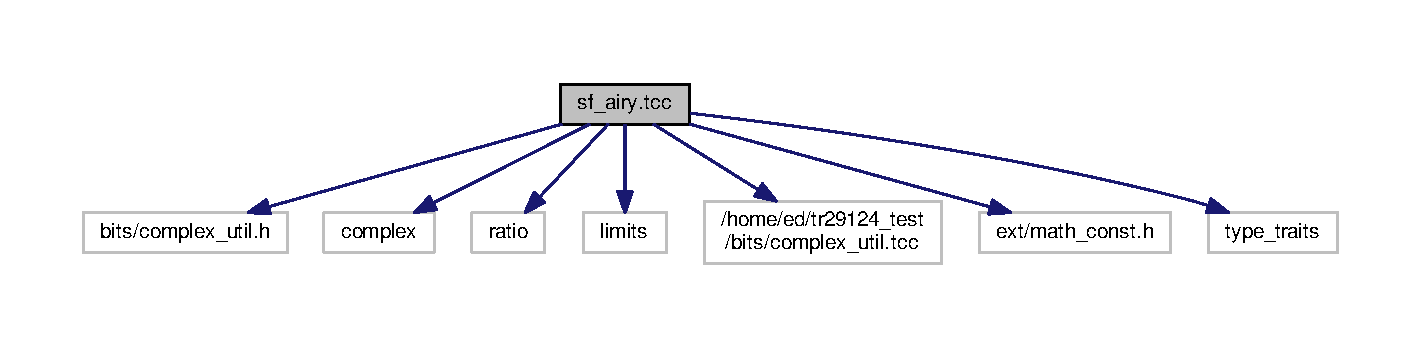
\includegraphics[width=350pt]{sf__airy_8tcc__incl}
\end{center}
\end{figure}
This graph shows which files directly or indirectly include this file\+:
\nopagebreak
\begin{figure}[H]
\begin{center}
\leavevmode
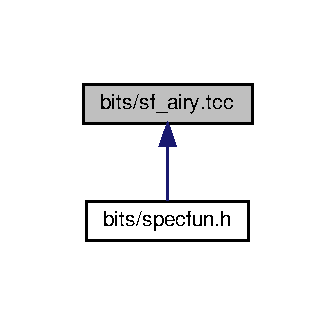
\includegraphics[width=161pt]{sf__airy_8tcc__dep__incl}
\end{center}
\end{figure}
\subsection*{Classes}
\begin{DoxyCompactItemize}
\item 
class \hyperlink{classstd_1_1____detail_1_1__Airy}{std\+::\+\_\+\+\_\+detail\+::\+\_\+\+Airy$<$ \+\_\+\+Tp $>$}
\item 
class \hyperlink{classstd_1_1____detail_1_1__Airy__asymp}{std\+::\+\_\+\+\_\+detail\+::\+\_\+\+Airy\+\_\+asymp$<$ \+\_\+\+Tp $>$}
\item 
struct \hyperlink{structstd_1_1____detail_1_1__Airy__asymp__data}{std\+::\+\_\+\+\_\+detail\+::\+\_\+\+Airy\+\_\+asymp\+\_\+data$<$ \+\_\+\+Tp $>$}
\item 
struct \hyperlink{structstd_1_1____detail_1_1__Airy__asymp__data_3_01double_01_4}{std\+::\+\_\+\+\_\+detail\+::\+\_\+\+Airy\+\_\+asymp\+\_\+data$<$ double $>$}
\item 
struct \hyperlink{structstd_1_1____detail_1_1__Airy__asymp__data_3_01float_01_4}{std\+::\+\_\+\+\_\+detail\+::\+\_\+\+Airy\+\_\+asymp\+\_\+data$<$ float $>$}
\item 
struct \hyperlink{structstd_1_1____detail_1_1__Airy__asymp__data_3_01long_01double_01_4}{std\+::\+\_\+\+\_\+detail\+::\+\_\+\+Airy\+\_\+asymp\+\_\+data$<$ long double $>$}
\item 
class \hyperlink{classstd_1_1____detail_1_1__Airy__asymp__series}{std\+::\+\_\+\+\_\+detail\+::\+\_\+\+Airy\+\_\+asymp\+\_\+series$<$ \+\_\+\+Sum $>$}
\item 
struct \hyperlink{structstd_1_1____detail_1_1__Airy__default__radii}{std\+::\+\_\+\+\_\+detail\+::\+\_\+\+Airy\+\_\+default\+\_\+radii$<$ \+\_\+\+Tp $>$}
\item 
struct \hyperlink{structstd_1_1____detail_1_1__Airy__default__radii_3_01double_01_4}{std\+::\+\_\+\+\_\+detail\+::\+\_\+\+Airy\+\_\+default\+\_\+radii$<$ double $>$}
\item 
struct \hyperlink{structstd_1_1____detail_1_1__Airy__default__radii_3_01float_01_4}{std\+::\+\_\+\+\_\+detail\+::\+\_\+\+Airy\+\_\+default\+\_\+radii$<$ float $>$}
\item 
struct \hyperlink{structstd_1_1____detail_1_1__Airy__default__radii_3_01long_01double_01_4}{std\+::\+\_\+\+\_\+detail\+::\+\_\+\+Airy\+\_\+default\+\_\+radii$<$ long double $>$}
\item 
class \hyperlink{classstd_1_1____detail_1_1__Airy__series}{std\+::\+\_\+\+\_\+detail\+::\+\_\+\+Airy\+\_\+series$<$ \+\_\+\+Tp $>$}
\item 
struct \hyperlink{structstd_1_1____detail_1_1__AiryAuxilliaryState}{std\+::\+\_\+\+\_\+detail\+::\+\_\+\+Airy\+Auxilliary\+State$<$ \+\_\+\+Tp $>$}
\item 
struct \hyperlink{structstd_1_1____detail_1_1__AiryState}{std\+::\+\_\+\+\_\+detail\+::\+\_\+\+Airy\+State$<$ \+\_\+\+Tp $>$}
\end{DoxyCompactItemize}
\subsection*{Namespaces}
\begin{DoxyCompactItemize}
\item 
 \hyperlink{namespacestd}{std}
\item 
 \hyperlink{namespacestd_1_1____detail}{std\+::\+\_\+\+\_\+detail}
\end{DoxyCompactItemize}
\subsection*{Macros}
\begin{DoxyCompactItemize}
\item 
\#define \hyperlink{sf__airy_8tcc_a2368d5b1edfb2e14f2c283d87ab89943}{\+\_\+\+G\+L\+I\+B\+C\+X\+X\+\_\+\+B\+I\+T\+S\+\_\+\+S\+F\+\_\+\+A\+I\+R\+Y\+\_\+\+T\+CC}~1
\end{DoxyCompactItemize}
\subsection*{Functions}
\begin{DoxyCompactItemize}
\item 
{\footnotesize template$<$typename \+\_\+\+Tp $>$ }\\std\+::complex$<$ \+\_\+\+Tp $>$ \hyperlink{namespacestd_1_1____detail_afd48b5702344f832a250922ac4ffb917}{std\+::\+\_\+\+\_\+detail\+::\+\_\+\+\_\+airy\+\_\+ai} (std\+::complex$<$ \+\_\+\+Tp $>$ \+\_\+\+\_\+z)
\begin{DoxyCompactList}\small\item\em Return the complex Airy Ai function. \end{DoxyCompactList}\item 
{\footnotesize template$<$typename \+\_\+\+Tp $>$ }\\std\+::complex$<$ \+\_\+\+Tp $>$ \hyperlink{namespacestd_1_1____detail_ae5536305d721e393efe1a74f0e57653e}{std\+::\+\_\+\+\_\+detail\+::\+\_\+\+\_\+airy\+\_\+bi} (std\+::complex$<$ \+\_\+\+Tp $>$ \+\_\+\+\_\+z)
\begin{DoxyCompactList}\small\item\em Return the complex Airy Bi function. \end{DoxyCompactList}\end{DoxyCompactItemize}
\subsection*{Variables}
\begin{DoxyCompactItemize}
\item 
{\footnotesize template$<$typename \+\_\+\+Tp $>$ }\\constexpr int \hyperlink{namespacestd_1_1____detail_ae3ef7007b55cd83fa162820c809a2995}{std\+::\+\_\+\+\_\+detail\+::\+\_\+\+\_\+max\+\_\+\+F\+GH} = \+\_\+\+Airy\+\_\+series$<$\+\_\+\+Tp$>$\+::\+\_\+\+N\+\_\+\+F\+GH
\item 
{\footnotesize template$<$$>$ }\\constexpr int \hyperlink{namespacestd_1_1____detail_ac945c3d1897eb356e75d379f67367a4b}{std\+::\+\_\+\+\_\+detail\+::\+\_\+\+\_\+max\+\_\+\+F\+G\+H$<$ double $>$} = 79
\item 
{\footnotesize template$<$$>$ }\\constexpr int \hyperlink{namespacestd_1_1____detail_a67195934ce49105fd7b765e669a5a2a0}{std\+::\+\_\+\+\_\+detail\+::\+\_\+\+\_\+max\+\_\+\+F\+G\+H$<$ float $>$} = 15
\end{DoxyCompactItemize}


\subsection{Detailed Description}
This is an internal header file, included by other library headers. You should not attempt to use it directly. 

\subsection{Macro Definition Documentation}
\mbox{\Hypertarget{sf__airy_8tcc_a2368d5b1edfb2e14f2c283d87ab89943}\label{sf__airy_8tcc_a2368d5b1edfb2e14f2c283d87ab89943}} 
\index{sf\+\_\+airy.\+tcc@{sf\+\_\+airy.\+tcc}!\+\_\+\+G\+L\+I\+B\+C\+X\+X\+\_\+\+B\+I\+T\+S\+\_\+\+S\+F\+\_\+\+A\+I\+R\+Y\+\_\+\+T\+CC@{\+\_\+\+G\+L\+I\+B\+C\+X\+X\+\_\+\+B\+I\+T\+S\+\_\+\+S\+F\+\_\+\+A\+I\+R\+Y\+\_\+\+T\+CC}}
\index{\+\_\+\+G\+L\+I\+B\+C\+X\+X\+\_\+\+B\+I\+T\+S\+\_\+\+S\+F\+\_\+\+A\+I\+R\+Y\+\_\+\+T\+CC@{\+\_\+\+G\+L\+I\+B\+C\+X\+X\+\_\+\+B\+I\+T\+S\+\_\+\+S\+F\+\_\+\+A\+I\+R\+Y\+\_\+\+T\+CC}!sf\+\_\+airy.\+tcc@{sf\+\_\+airy.\+tcc}}
\subsubsection{\texorpdfstring{\+\_\+\+G\+L\+I\+B\+C\+X\+X\+\_\+\+B\+I\+T\+S\+\_\+\+S\+F\+\_\+\+A\+I\+R\+Y\+\_\+\+T\+CC}{\_GLIBCXX\_BITS\_SF\_AIRY\_TCC}}
{\footnotesize\ttfamily \#define \+\_\+\+G\+L\+I\+B\+C\+X\+X\+\_\+\+B\+I\+T\+S\+\_\+\+S\+F\+\_\+\+A\+I\+R\+Y\+\_\+\+T\+CC~1}



Definition at line 31 of file sf\+\_\+airy.\+tcc.


\hypertarget{sf__bessel_8tcc}{}\doxysection{cxx\+\_\+special\+\_\+functions/include/emsr/detail/sf\+\_\+bessel.tcc File Reference}
\label{sf__bessel_8tcc}\index{cxx\_special\_functions/include/emsr/detail/sf\_bessel.tcc@{cxx\_special\_functions/include/emsr/detail/sf\_bessel.tcc}}
{\ttfamily \#include $<$stdexcept$>$}\newline
{\ttfamily \#include $<$complex$>$}\newline
{\ttfamily \#include $<$utility$>$}\newline
{\ttfamily \#include $<$emsr/fp\+\_\+type\+\_\+util.\+h$>$}\newline
{\ttfamily \#include $<$emsr/sf\+\_\+trig.\+h$>$}\newline
{\ttfamily \#include $<$emsr/sf\+\_\+gamma.\+h$>$}\newline
{\ttfamily \#include $<$emsr/specfun\+\_\+state.\+h$>$}\newline
Include dependency graph for sf\+\_\+bessel.\+tcc\+:
\nopagebreak
\begin{figure}[H]
\begin{center}
\leavevmode
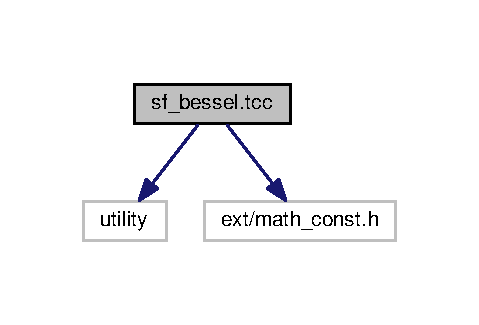
\includegraphics[width=350pt]{sf__bessel_8tcc__incl}
\end{center}
\end{figure}
\doxysubsection*{Classes}
\begin{DoxyCompactItemize}
\item 
struct \mbox{\hyperlink{structemsr_1_1detail_1_1cyl__bessel__asymp__sums__t}{emsr\+::detail\+::cyl\+\_\+bessel\+\_\+asymp\+\_\+sums\+\_\+t$<$ Tnu, Tp $>$}}
\end{DoxyCompactItemize}
\doxysubsection*{Namespaces}
\begin{DoxyCompactItemize}
\item 
 \mbox{\hyperlink{namespaceemsr}{emsr}}
\item 
 \mbox{\hyperlink{namespaceemsr_1_1detail}{emsr\+::detail}}
\end{DoxyCompactItemize}
\doxysubsection*{Macros}
\begin{DoxyCompactItemize}
\item 
\#define \mbox{\hyperlink{sf__bessel_8tcc_a49e12b0a9815fd538fa167d74744ac70}{SF\+\_\+\+BESSEL\+\_\+\+TCC}}~1
\end{DoxyCompactItemize}
\doxysubsection*{Functions}
\begin{DoxyCompactItemize}
\item 
{\footnotesize template$<$typename Tnu , typename Tp $>$ }\\constexpr cyl\+\_\+bessel\+\_\+asymp\+\_\+sums\+\_\+t$<$ Tnu, Tp $>$ \mbox{\hyperlink{namespaceemsr_1_1detail_a4ad1dd069e3e9d6c215c5edd76d28c08}{emsr\+::detail\+::cyl\+\_\+bessel\+\_\+asymp\+\_\+sums}} (Tnu nu, Tp x, int sgn)
\begin{DoxyCompactList}\small\item\em This routine computes the asymptotic cylindrical Bessel and Neumann functions of order nu\+: $ J_{\nu}(z) $, $ N_{\nu}(z) $. Use this for $ z >> \nu^2 + 1 $. \end{DoxyCompactList}\item 
{\footnotesize template$<$typename Tnu , typename Tp $>$ }\\constexpr Tp \mbox{\hyperlink{namespaceemsr_1_1detail_a5d03a25e93fe8101a8bc797599996593}{emsr\+::detail\+::cyl\+\_\+bessel\+\_\+ij\+\_\+series}} (Tnu nu, Tp x, int sgn, unsigned int max\+\_\+iter)
\begin{DoxyCompactList}\small\item\em This routine returns the cylindrical Bessel functions of order $ \nu $\+: $ J_{\nu}(z) $ or $ I_{\nu}(z) $ by series expansion. \end{DoxyCompactList}\item 
{\footnotesize template$<$typename Tp $>$ }\\Tp \mbox{\hyperlink{namespaceemsr_1_1detail_a709966a51624f7bcd044833c2a9496b3}{emsr\+::detail\+::cyl\+\_\+bessel\+\_\+j}} (Tp nu, Tp x)
\begin{DoxyCompactList}\small\item\em Return the Bessel function of order $ \nu $\+: $ J_{\nu}(x) $. \end{DoxyCompactList}\item 
{\footnotesize template$<$typename Tp $>$ }\\\mbox{\hyperlink{structemsr_1_1cyl__bessel__t}{emsr\+::cyl\+\_\+bessel\+\_\+t}}$<$ Tp, Tp, Tp $>$ \mbox{\hyperlink{namespaceemsr_1_1detail_a2b475478f0b1a13817ee037b151e45b2}{emsr\+::detail\+::cyl\+\_\+bessel\+\_\+jn}} (Tp nu, Tp x)
\begin{DoxyCompactList}\small\item\em Return the cylindrical Bessel functions and their derivatives of order $ \nu $ by various means. \end{DoxyCompactList}\item 
{\footnotesize template$<$typename Tnu , typename Tp $>$ }\\constexpr \mbox{\hyperlink{structemsr_1_1cyl__bessel__t}{emsr\+::cyl\+\_\+bessel\+\_\+t}}$<$ Tnu, Tp, Tp $>$ \mbox{\hyperlink{namespaceemsr_1_1detail_a881c494d0a399876fbe730b2e943027d}{emsr\+::detail\+::cyl\+\_\+bessel\+\_\+jn\+\_\+asymp}} (Tnu nu, Tp x)
\item 
{\footnotesize template$<$typename Tp $>$ }\\\mbox{\hyperlink{structemsr_1_1cyl__bessel__t}{emsr\+::cyl\+\_\+bessel\+\_\+t}}$<$ Tp, Tp, std\+::complex$<$ Tp $>$ $>$ \mbox{\hyperlink{namespaceemsr_1_1detail_a29bd2b06ad129a73e01293b7464bf5f6}{emsr\+::detail\+::cyl\+\_\+bessel\+\_\+jn\+\_\+neg\+\_\+arg}} (Tp nu, Tp x)
\begin{DoxyCompactList}\small\item\em Return the cylindrical Bessel functions and their derivatives of real order $ \nu $ and argument $ x < 0 $. \end{DoxyCompactList}\item 
{\footnotesize template$<$typename Tp $>$ }\\\mbox{\hyperlink{structemsr_1_1cyl__bessel__t}{emsr\+::cyl\+\_\+bessel\+\_\+t}}$<$ Tp, Tp, Tp $>$ \mbox{\hyperlink{namespaceemsr_1_1detail_a8a51a911f442ca85bddda5a77586e728}{emsr\+::detail\+::cyl\+\_\+bessel\+\_\+jn\+\_\+steed}} (Tp nu, Tp x)
\begin{DoxyCompactList}\small\item\em Compute the Bessel $ J_\nu(x) $ and Neumann $ N_\nu(x) $ functions and their first derivatives $ J\textnormal{\textquotesingle}_\nu(x) $ and $ N\textnormal{\textquotesingle}_\nu(x) $ respectively. These four functions are computed together for numerical stability. \end{DoxyCompactList}\item 
{\footnotesize template$<$typename Tp $>$ }\\std\+::complex$<$ Tp $>$ \mbox{\hyperlink{namespaceemsr_1_1detail_abaedaeed2f648c65d105d7f9c7a74ace}{emsr\+::detail\+::cyl\+\_\+hankel\+\_\+1}} (Tp nu, Tp x)
\begin{DoxyCompactList}\small\item\em Return the cylindrical Hankel function of the first kind $ H^{(1)}_\nu(x) $. \end{DoxyCompactList}\item 
{\footnotesize template$<$typename Tp $>$ }\\std\+::complex$<$ Tp $>$ \mbox{\hyperlink{namespaceemsr_1_1detail_ad994a797a9b890863bcbc80b77b34896}{emsr\+::detail\+::cyl\+\_\+hankel\+\_\+2}} (Tp nu, Tp x)
\begin{DoxyCompactList}\small\item\em Return the cylindrical Hankel function of the second kind $ H^{(2)}_nu(x) $. \end{DoxyCompactList}\item 
{\footnotesize template$<$typename Tp $>$ }\\\mbox{\hyperlink{structemsr_1_1cyl__hankel__t}{emsr\+::cyl\+\_\+hankel\+\_\+t}}$<$ Tp, Tp, std\+::complex$<$ Tp $>$ $>$ \mbox{\hyperlink{namespaceemsr_1_1detail_aff5286a95ad2c869f273d86f3614459e}{emsr\+::detail\+::cyl\+\_\+hankel\+\_\+h1h2}} (Tp nu, Tp x)
\begin{DoxyCompactList}\small\item\em Return the cylindrical Hankel functions of the first and second kinds and their derivatives. \end{DoxyCompactList}\item 
{\footnotesize template$<$typename Tp $>$ }\\Tp \mbox{\hyperlink{namespaceemsr_1_1detail_a9c5b42d7e62f5509f2d024d2b63bac65}{emsr\+::detail\+::cyl\+\_\+neumann\+\_\+n}} (Tp nu, Tp x)
\begin{DoxyCompactList}\small\item\em Return the Neumann function of order $ \nu $\+: $ N_{\nu}(x) $. \end{DoxyCompactList}\item 
{\footnotesize template$<$typename Tp $>$ }\\\mbox{\hyperlink{structemsr_1_1gamma__temme__t}{emsr\+::gamma\+\_\+temme\+\_\+t}}$<$ Tp $>$ \mbox{\hyperlink{namespaceemsr_1_1detail_a9fb4df348835eb89968e74318bd6725a}{emsr\+::detail\+::gamma\+\_\+temme}} (Tp mu)
\begin{DoxyCompactList}\small\item\em Compute the gamma functions required by the Temme series expansions of $ N_\nu(x) $ and $ K_\nu(x) $. \end{DoxyCompactList}\item 
{\footnotesize template$<$typename Tp $>$ }\\Tp \mbox{\hyperlink{namespaceemsr_1_1detail_a23a8ccedae862a9760f0e316e19b8e6d}{emsr\+::detail\+::sph\+\_\+bessel}} (unsigned int n, Tp x)
\begin{DoxyCompactList}\small\item\em Return the spherical Bessel function $ j_n(x) $ of order n and non-\/negative real argument {\ttfamily x}. \end{DoxyCompactList}\item 
{\footnotesize template$<$typename Tp $>$ }\\\mbox{\hyperlink{structemsr_1_1sph__bessel__t}{emsr\+::sph\+\_\+bessel\+\_\+t}}$<$ unsigned int, Tp, Tp $>$ \mbox{\hyperlink{namespaceemsr_1_1detail_ad40906b9a4b03719aff5ab33e87dbd31}{emsr\+::detail\+::sph\+\_\+bessel\+\_\+jn}} (unsigned int n, Tp x)
\begin{DoxyCompactList}\small\item\em Compute the spherical Bessel $ j_n(x) $ and Neumann $ n_n(x) $ functions and their first derivatives $ j_n(x) $ and $ n\textnormal{\textquotesingle}_n(x) $ respectively. \end{DoxyCompactList}\item 
{\footnotesize template$<$typename Tp $>$ }\\\mbox{\hyperlink{structemsr_1_1sph__bessel__t}{emsr\+::sph\+\_\+bessel\+\_\+t}}$<$ unsigned int, Tp, std\+::complex$<$ Tp $>$ $>$ \mbox{\hyperlink{namespaceemsr_1_1detail_af9c2d74a618891f01695f955bd3ebea1}{emsr\+::detail\+::sph\+\_\+bessel\+\_\+jn\+\_\+neg\+\_\+arg}} (unsigned int n, Tp x)
\item 
{\footnotesize template$<$typename Tp $>$ }\\std\+::complex$<$ Tp $>$ \mbox{\hyperlink{namespaceemsr_1_1detail_ad6eea5d6cf9ed96b912e4c8cda769644}{emsr\+::detail\+::sph\+\_\+hankel\+\_\+1}} (unsigned int n, Tp x)
\begin{DoxyCompactList}\small\item\em Return the spherical Hankel function of the first kind $ h^{(1)}_n(x) $. \end{DoxyCompactList}\item 
{\footnotesize template$<$typename Tp $>$ }\\std\+::complex$<$ Tp $>$ \mbox{\hyperlink{namespaceemsr_1_1detail_ae1f76cc000aedd6726c5bdcbb5337381}{emsr\+::detail\+::sph\+\_\+hankel\+\_\+2}} (unsigned int n, Tp x)
\begin{DoxyCompactList}\small\item\em Return the spherical Hankel function of the second kind $ h^{(2)}_n(x) $. \end{DoxyCompactList}\item 
{\footnotesize template$<$typename Tp $>$ }\\Tp \mbox{\hyperlink{namespaceemsr_1_1detail_a7f7eea7c7380172a93d9dfb45acf3a2a}{emsr\+::detail\+::sph\+\_\+neumann}} (unsigned int n, Tp x)
\begin{DoxyCompactList}\small\item\em Return the spherical Neumann function $ n_n(x) $ of order n and non-\/negative real argument {\ttfamily x}. \end{DoxyCompactList}\end{DoxyCompactItemize}


\doxysubsection{Macro Definition Documentation}
\mbox{\Hypertarget{sf__bessel_8tcc_a49e12b0a9815fd538fa167d74744ac70}\label{sf__bessel_8tcc_a49e12b0a9815fd538fa167d74744ac70}} 
\index{sf\_bessel.tcc@{sf\_bessel.tcc}!SF\_BESSEL\_TCC@{SF\_BESSEL\_TCC}}
\index{SF\_BESSEL\_TCC@{SF\_BESSEL\_TCC}!sf\_bessel.tcc@{sf\_bessel.tcc}}
\doxysubsubsection{\texorpdfstring{SF\_BESSEL\_TCC}{SF\_BESSEL\_TCC}}
{\footnotesize\ttfamily \#define SF\+\_\+\+BESSEL\+\_\+\+TCC~1}



Definition at line 46 of file sf\+\_\+bessel.\+tcc.


\hypertarget{sf__beta_8tcc}{}\section{include/bits/sf\+\_\+beta.tcc File Reference}
\label{sf__beta_8tcc}\index{include/bits/sf\+\_\+beta.\+tcc@{include/bits/sf\+\_\+beta.\+tcc}}
{\ttfamily \#include $<$ext/math\+\_\+const.\+h$>$}\newline
Include dependency graph for sf\+\_\+beta.\+tcc\+:
\nopagebreak
\begin{figure}[H]
\begin{center}
\leavevmode
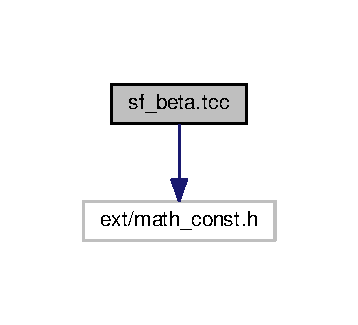
\includegraphics[width=198pt]{sf__beta_8tcc__incl}
\end{center}
\end{figure}
This graph shows which files directly or indirectly include this file\+:
\nopagebreak
\begin{figure}[H]
\begin{center}
\leavevmode
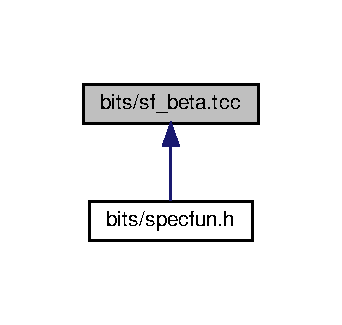
\includegraphics[width=198pt]{sf__beta_8tcc__dep__incl}
\end{center}
\end{figure}
\subsection*{Namespaces}
\begin{DoxyCompactItemize}
\item 
 \hyperlink{namespacestd}{std}
\item 
 \hyperlink{namespacestd_1_1____detail}{std\+::\+\_\+\+\_\+detail}
\begin{DoxyCompactList}\small\item\em Implementation-\/space details. \end{DoxyCompactList}\end{DoxyCompactItemize}
\subsection*{Macros}
\begin{DoxyCompactItemize}
\item 
\#define \hyperlink{sf__beta_8tcc_a41fb0de3283ace5ea2b676d932ff3d32}{\+\_\+\+G\+L\+I\+B\+C\+X\+X\+\_\+\+B\+I\+T\+S\+\_\+\+S\+F\+\_\+\+B\+E\+T\+A\+\_\+\+T\+CC}~1
\end{DoxyCompactItemize}
\subsection*{Functions}
\begin{DoxyCompactItemize}
\item 
{\footnotesize template$<$typename \+\_\+\+Tp $>$ }\\\+\_\+\+Tp \hyperlink{namespacestd_1_1____detail_a090d2f0920e0d208c467609b2a81d717}{std\+::\+\_\+\+\_\+detail\+::\+\_\+\+\_\+beta} (\+\_\+\+Tp \+\_\+\+\_\+a, \+\_\+\+Tp \+\_\+\+\_\+b)
\begin{DoxyCompactList}\small\item\em Return the beta function $ B(a,b) $. \end{DoxyCompactList}\item 
{\footnotesize template$<$typename \+\_\+\+Tp $>$ }\\\+\_\+\+Tp \hyperlink{namespacestd_1_1____detail_a93cfa67cc3f14564925ed3153e055cd1}{std\+::\+\_\+\+\_\+detail\+::\+\_\+\+\_\+beta\+\_\+gamma} (\+\_\+\+Tp \+\_\+\+\_\+a, \+\_\+\+Tp \+\_\+\+\_\+b)
\begin{DoxyCompactList}\small\item\em Return the beta function\+: $ B(a,b) $. \end{DoxyCompactList}\item 
{\footnotesize template$<$typename \+\_\+\+Tp $>$ }\\\+\_\+\+Tp \hyperlink{namespacestd_1_1____detail_aedfe43a9c0065cc3883df50536a625e4}{std\+::\+\_\+\+\_\+detail\+::\+\_\+\+\_\+beta\+\_\+inc} (\+\_\+\+Tp \+\_\+\+\_\+a, \+\_\+\+Tp \+\_\+\+\_\+b, \+\_\+\+Tp \+\_\+\+\_\+x)
\item 
{\footnotesize template$<$typename \+\_\+\+Tp $>$ }\\\+\_\+\+Tp \hyperlink{namespacestd_1_1____detail_ac4f233100713779d93e4eee7665bd0a5}{std\+::\+\_\+\+\_\+detail\+::\+\_\+\+\_\+beta\+\_\+lgamma} (\+\_\+\+Tp \+\_\+\+\_\+a, \+\_\+\+Tp \+\_\+\+\_\+b)
\begin{DoxyCompactList}\small\item\em Return the beta function $B(a,b)$ using the log gamma functions. \end{DoxyCompactList}\item 
{\footnotesize template$<$typename \+\_\+\+Tp $>$ }\\\+\_\+\+Tp \hyperlink{namespacestd_1_1____detail_a9baa688a27befab7fa48ccfb4a87a9ca}{std\+::\+\_\+\+\_\+detail\+::\+\_\+\+\_\+beta\+\_\+product} (\+\_\+\+Tp \+\_\+\+\_\+a, \+\_\+\+Tp \+\_\+\+\_\+b)
\begin{DoxyCompactList}\small\item\em Return the beta function $B(x,y)$ using the product form. \end{DoxyCompactList}\item 
{\footnotesize template$<$typename \+\_\+\+Tp $>$ }\\\+\_\+\+Tp \hyperlink{namespacestd_1_1____detail_a96a5a5205553de07f98b89b2e1f18000}{std\+::\+\_\+\+\_\+detail\+::\+\_\+\+\_\+ibeta\+\_\+cont\+\_\+frac} (\+\_\+\+Tp \+\_\+\+\_\+a, \+\_\+\+Tp \+\_\+\+\_\+b, \+\_\+\+Tp \+\_\+\+\_\+x)
\end{DoxyCompactItemize}


\subsection{Detailed Description}
This is an internal header file, included by other library headers. Do not attempt to use it directly. Instead, include $<$cmath$>$. 

\subsection{Macro Definition Documentation}
\mbox{\Hypertarget{sf__beta_8tcc_a41fb0de3283ace5ea2b676d932ff3d32}\label{sf__beta_8tcc_a41fb0de3283ace5ea2b676d932ff3d32}} 
\index{sf\+\_\+beta.\+tcc@{sf\+\_\+beta.\+tcc}!\+\_\+\+G\+L\+I\+B\+C\+X\+X\+\_\+\+B\+I\+T\+S\+\_\+\+S\+F\+\_\+\+B\+E\+T\+A\+\_\+\+T\+CC@{\+\_\+\+G\+L\+I\+B\+C\+X\+X\+\_\+\+B\+I\+T\+S\+\_\+\+S\+F\+\_\+\+B\+E\+T\+A\+\_\+\+T\+CC}}
\index{\+\_\+\+G\+L\+I\+B\+C\+X\+X\+\_\+\+B\+I\+T\+S\+\_\+\+S\+F\+\_\+\+B\+E\+T\+A\+\_\+\+T\+CC@{\+\_\+\+G\+L\+I\+B\+C\+X\+X\+\_\+\+B\+I\+T\+S\+\_\+\+S\+F\+\_\+\+B\+E\+T\+A\+\_\+\+T\+CC}!sf\+\_\+beta.\+tcc@{sf\+\_\+beta.\+tcc}}
\subsubsection{\texorpdfstring{\+\_\+\+G\+L\+I\+B\+C\+X\+X\+\_\+\+B\+I\+T\+S\+\_\+\+S\+F\+\_\+\+B\+E\+T\+A\+\_\+\+T\+CC}{\_GLIBCXX\_BITS\_SF\_BETA\_TCC}}
{\footnotesize\ttfamily \#define \+\_\+\+G\+L\+I\+B\+C\+X\+X\+\_\+\+B\+I\+T\+S\+\_\+\+S\+F\+\_\+\+B\+E\+T\+A\+\_\+\+T\+CC~1}



Definition at line 49 of file sf\+\_\+beta.\+tcc.


\hypertarget{sf__cardinal_8tcc}{}\section{bits/sf\+\_\+cardinal.tcc File Reference}
\label{sf__cardinal_8tcc}\index{bits/sf\+\_\+cardinal.\+tcc@{bits/sf\+\_\+cardinal.\+tcc}}
{\ttfamily \#include $<$bits/complex\+\_\+util.\+h$>$}\\*
Include dependency graph for sf\+\_\+cardinal.\+tcc\+:
\nopagebreak
\begin{figure}[H]
\begin{center}
\leavevmode
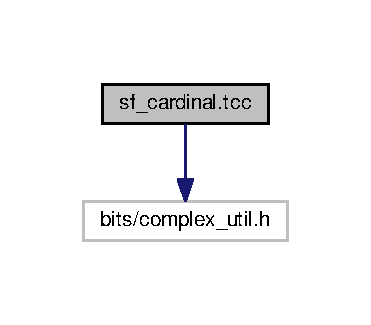
\includegraphics[width=179pt]{sf__cardinal_8tcc__incl}
\end{center}
\end{figure}
This graph shows which files directly or indirectly include this file\+:
\nopagebreak
\begin{figure}[H]
\begin{center}
\leavevmode
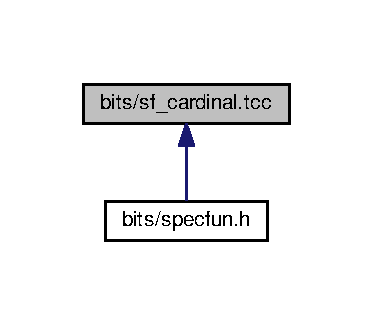
\includegraphics[width=179pt]{sf__cardinal_8tcc__dep__incl}
\end{center}
\end{figure}
\subsection*{Namespaces}
\begin{DoxyCompactItemize}
\item 
 \hyperlink{namespacestd}{std}
\item 
 \hyperlink{namespacestd_1_1____detail}{std\+::\+\_\+\+\_\+detail}
\end{DoxyCompactItemize}
\subsection*{Macros}
\begin{DoxyCompactItemize}
\item 
\#define \hyperlink{sf__cardinal_8tcc_a1e9bb8201f62b2303ba941ea920790b6}{\+\_\+\+G\+L\+I\+B\+C\+X\+X\+\_\+\+B\+I\+T\+S\+\_\+\+S\+F\+\_\+\+C\+A\+R\+D\+I\+N\+A\+L\+\_\+\+T\+CC}~1
\end{DoxyCompactItemize}
\subsection*{Functions}
\begin{DoxyCompactItemize}
\item 
{\footnotesize template$<$typename \+\_\+\+Tp $>$ }\\\+\_\+\+\_\+gnu\+\_\+cxx\+::\+\_\+\+\_\+promote\+\_\+fp\+\_\+t$<$ \+\_\+\+Tp $>$ \hyperlink{namespacestd_1_1____detail_aa7bdd4dd998288441b84ca2e142a4a04}{std\+::\+\_\+\+\_\+detail\+::\+\_\+\+\_\+sinc} (\+\_\+\+Tp \+\_\+\+\_\+x)
\begin{DoxyCompactList}\small\item\em Return the sinus cardinal function \[ sinc(x) = \frac{\sin(x)}{x} \]. \end{DoxyCompactList}\item 
{\footnotesize template$<$typename \+\_\+\+Tp $>$ }\\\+\_\+\+\_\+gnu\+\_\+cxx\+::\+\_\+\+\_\+promote\+\_\+fp\+\_\+t$<$ \+\_\+\+Tp $>$ \hyperlink{namespacestd_1_1____detail_accfe65ec3790f60b0b429afbd4000bb1}{std\+::\+\_\+\+\_\+detail\+::\+\_\+\+\_\+sinc\+\_\+pi} (\+\_\+\+Tp \+\_\+\+\_\+x)
\begin{DoxyCompactList}\small\item\em Return the reperiodized sinus cardinal function \[ sinc_\pi(x) = \frac{\sin(\pi x)}{\pi x} \]. \end{DoxyCompactList}\item 
{\footnotesize template$<$typename \+\_\+\+Tp $>$ }\\\+\_\+\+\_\+gnu\+\_\+cxx\+::\+\_\+\+\_\+promote\+\_\+fp\+\_\+t$<$ \+\_\+\+Tp $>$ \hyperlink{namespacestd_1_1____detail_a542bbc5f25643898444c02fbaec5c820}{std\+::\+\_\+\+\_\+detail\+::\+\_\+\+\_\+sinhc} (\+\_\+\+Tp \+\_\+\+\_\+x)
\begin{DoxyCompactList}\small\item\em Return the hyperbolic sinus cardinal function \[ sinhc(x) = \frac{\sinh(x)}{x} \]. \end{DoxyCompactList}\item 
{\footnotesize template$<$typename \+\_\+\+Tp $>$ }\\\+\_\+\+\_\+gnu\+\_\+cxx\+::\+\_\+\+\_\+promote\+\_\+fp\+\_\+t$<$ \+\_\+\+Tp $>$ \hyperlink{namespacestd_1_1____detail_adcb7d17819902a9b4fa0bd5543dd3f6b}{std\+::\+\_\+\+\_\+detail\+::\+\_\+\+\_\+sinhc\+\_\+pi} (\+\_\+\+Tp \+\_\+\+\_\+x)
\begin{DoxyCompactList}\small\item\em Return the reperiodized hyperbolic sinus cardinal function \[ sinhc_\pi(x) = \frac{\sinh(\pi x)}{\pi x} \]. \end{DoxyCompactList}\end{DoxyCompactItemize}


\subsection{Macro Definition Documentation}
\index{sf\+\_\+cardinal.\+tcc@{sf\+\_\+cardinal.\+tcc}!\+\_\+\+G\+L\+I\+B\+C\+X\+X\+\_\+\+B\+I\+T\+S\+\_\+\+S\+F\+\_\+\+C\+A\+R\+D\+I\+N\+A\+L\+\_\+\+T\+CC@{\+\_\+\+G\+L\+I\+B\+C\+X\+X\+\_\+\+B\+I\+T\+S\+\_\+\+S\+F\+\_\+\+C\+A\+R\+D\+I\+N\+A\+L\+\_\+\+T\+CC}}
\index{\+\_\+\+G\+L\+I\+B\+C\+X\+X\+\_\+\+B\+I\+T\+S\+\_\+\+S\+F\+\_\+\+C\+A\+R\+D\+I\+N\+A\+L\+\_\+\+T\+CC@{\+\_\+\+G\+L\+I\+B\+C\+X\+X\+\_\+\+B\+I\+T\+S\+\_\+\+S\+F\+\_\+\+C\+A\+R\+D\+I\+N\+A\+L\+\_\+\+T\+CC}!sf\+\_\+cardinal.\+tcc@{sf\+\_\+cardinal.\+tcc}}
\subsubsection[{\texorpdfstring{\+\_\+\+G\+L\+I\+B\+C\+X\+X\+\_\+\+B\+I\+T\+S\+\_\+\+S\+F\+\_\+\+C\+A\+R\+D\+I\+N\+A\+L\+\_\+\+T\+CC}{_GLIBCXX_BITS_SF_CARDINAL_TCC}}]{\setlength{\rightskip}{0pt plus 5cm}\#define \+\_\+\+G\+L\+I\+B\+C\+X\+X\+\_\+\+B\+I\+T\+S\+\_\+\+S\+F\+\_\+\+C\+A\+R\+D\+I\+N\+A\+L\+\_\+\+T\+CC~1}\hypertarget{sf__cardinal_8tcc_a1e9bb8201f62b2303ba941ea920790b6}{}\label{sf__cardinal_8tcc_a1e9bb8201f62b2303ba941ea920790b6}


Definition at line 31 of file sf\+\_\+cardinal.\+tcc.


\hypertarget{sf__chebyshev_8tcc}{}\section{bits/sf\+\_\+chebyshev.tcc File Reference}
\label{sf__chebyshev_8tcc}\index{bits/sf\+\_\+chebyshev.\+tcc@{bits/sf\+\_\+chebyshev.\+tcc}}
{\ttfamily \#include $<$ext/math\+\_\+const.\+h$>$}\\*
Include dependency graph for sf\+\_\+chebyshev.\+tcc\+:
\nopagebreak
\begin{figure}[H]
\begin{center}
\leavevmode
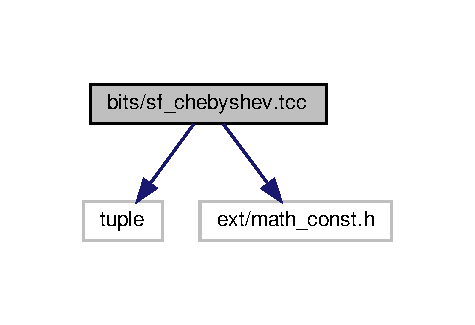
\includegraphics[width=193pt]{sf__chebyshev_8tcc__incl}
\end{center}
\end{figure}
This graph shows which files directly or indirectly include this file\+:
\nopagebreak
\begin{figure}[H]
\begin{center}
\leavevmode
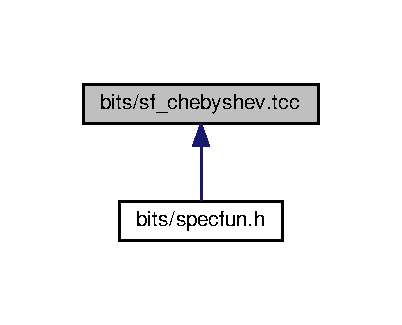
\includegraphics[width=193pt]{sf__chebyshev_8tcc__dep__incl}
\end{center}
\end{figure}
\subsection*{Namespaces}
\begin{DoxyCompactItemize}
\item 
 \hyperlink{namespacestd}{std}
\item 
 \hyperlink{namespacestd_1_1____detail}{std\+::\+\_\+\+\_\+detail}
\end{DoxyCompactItemize}
\subsection*{Macros}
\begin{DoxyCompactItemize}
\item 
\#define \hyperlink{sf__chebyshev_8tcc_af93a8a3778aadae3937c7f4b1aa86123}{\+\_\+\+G\+L\+I\+B\+C\+X\+X\+\_\+\+B\+I\+T\+S\+\_\+\+S\+F\+\_\+\+C\+H\+E\+B\+Y\+S\+H\+E\+V\+\_\+\+T\+CC}~1
\end{DoxyCompactItemize}
\subsection*{Functions}
\begin{DoxyCompactItemize}
\item 
{\footnotesize template$<$typename \+\_\+\+Tp $>$ }\\\+\_\+\+Tp \hyperlink{namespacestd_1_1____detail_a3a893b4c60f3245af5db4ca792c4b2cf}{std\+::\+\_\+\+\_\+detail\+::\+\_\+\+\_\+chebyshev\+\_\+recur} (unsigned int \+\_\+\+\_\+n, \+\_\+\+Tp \+\_\+\+\_\+x, \+\_\+\+Tp \+\_\+\+C0, \+\_\+\+Tp \+\_\+\+C1)
\item 
{\footnotesize template$<$typename \+\_\+\+Tp $>$ }\\\+\_\+\+Tp \hyperlink{namespacestd_1_1____detail_af4ba1015e914cdd23d9e5d2be69740c1}{std\+::\+\_\+\+\_\+detail\+::\+\_\+\+\_\+chebyshev\+\_\+t} (unsigned int \+\_\+\+\_\+n, \+\_\+\+Tp \+\_\+\+\_\+x)
\item 
{\footnotesize template$<$typename \+\_\+\+Tp $>$ }\\\+\_\+\+Tp \hyperlink{namespacestd_1_1____detail_aa3289db0a53f55007bc10dc94f15c1f7}{std\+::\+\_\+\+\_\+detail\+::\+\_\+\+\_\+chebyshev\+\_\+u} (unsigned int \+\_\+\+\_\+n, \+\_\+\+Tp \+\_\+\+\_\+x)
\item 
{\footnotesize template$<$typename \+\_\+\+Tp $>$ }\\\+\_\+\+Tp \hyperlink{namespacestd_1_1____detail_a684b312a311bbe2065a2633220f4507d}{std\+::\+\_\+\+\_\+detail\+::\+\_\+\+\_\+chebyshev\+\_\+v} (unsigned int \+\_\+\+\_\+n, \+\_\+\+Tp \+\_\+\+\_\+x)
\item 
{\footnotesize template$<$typename \+\_\+\+Tp $>$ }\\\+\_\+\+Tp \hyperlink{namespacestd_1_1____detail_ae220390e755bdc4908e040fd68426d14}{std\+::\+\_\+\+\_\+detail\+::\+\_\+\+\_\+chebyshev\+\_\+w} (unsigned int \+\_\+\+\_\+n, \+\_\+\+Tp \+\_\+\+\_\+x)
\end{DoxyCompactItemize}


\subsection{Detailed Description}
This is an internal header file, included by other library headers. Do not attempt to use it directly. Instead, include $<$cmath$>$. 

\subsection{Macro Definition Documentation}
\index{sf\+\_\+chebyshev.\+tcc@{sf\+\_\+chebyshev.\+tcc}!\+\_\+\+G\+L\+I\+B\+C\+X\+X\+\_\+\+B\+I\+T\+S\+\_\+\+S\+F\+\_\+\+C\+H\+E\+B\+Y\+S\+H\+E\+V\+\_\+\+T\+CC@{\+\_\+\+G\+L\+I\+B\+C\+X\+X\+\_\+\+B\+I\+T\+S\+\_\+\+S\+F\+\_\+\+C\+H\+E\+B\+Y\+S\+H\+E\+V\+\_\+\+T\+CC}}
\index{\+\_\+\+G\+L\+I\+B\+C\+X\+X\+\_\+\+B\+I\+T\+S\+\_\+\+S\+F\+\_\+\+C\+H\+E\+B\+Y\+S\+H\+E\+V\+\_\+\+T\+CC@{\+\_\+\+G\+L\+I\+B\+C\+X\+X\+\_\+\+B\+I\+T\+S\+\_\+\+S\+F\+\_\+\+C\+H\+E\+B\+Y\+S\+H\+E\+V\+\_\+\+T\+CC}!sf\+\_\+chebyshev.\+tcc@{sf\+\_\+chebyshev.\+tcc}}
\subsubsection[{\texorpdfstring{\+\_\+\+G\+L\+I\+B\+C\+X\+X\+\_\+\+B\+I\+T\+S\+\_\+\+S\+F\+\_\+\+C\+H\+E\+B\+Y\+S\+H\+E\+V\+\_\+\+T\+CC}{_GLIBCXX_BITS_SF_CHEBYSHEV_TCC}}]{\setlength{\rightskip}{0pt plus 5cm}\#define \+\_\+\+G\+L\+I\+B\+C\+X\+X\+\_\+\+B\+I\+T\+S\+\_\+\+S\+F\+\_\+\+C\+H\+E\+B\+Y\+S\+H\+E\+V\+\_\+\+T\+CC~1}\hypertarget{sf__chebyshev_8tcc_af93a8a3778aadae3937c7f4b1aa86123}{}\label{sf__chebyshev_8tcc_af93a8a3778aadae3937c7f4b1aa86123}


Definition at line 31 of file sf\+\_\+chebyshev.\+tcc.


\hypertarget{sf__dawson_8tcc}{}\section{bits/sf\+\_\+dawson.tcc File Reference}
\label{sf__dawson_8tcc}\index{bits/sf\+\_\+dawson.\+tcc@{bits/sf\+\_\+dawson.\+tcc}}
{\ttfamily \#include $<$ext/math\+\_\+const.\+h$>$}\\*
Include dependency graph for sf\+\_\+dawson.\+tcc\+:
\nopagebreak
\begin{figure}[H]
\begin{center}
\leavevmode
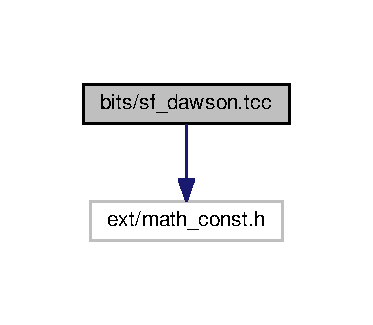
\includegraphics[width=179pt]{sf__dawson_8tcc__incl}
\end{center}
\end{figure}
This graph shows which files directly or indirectly include this file\+:
\nopagebreak
\begin{figure}[H]
\begin{center}
\leavevmode
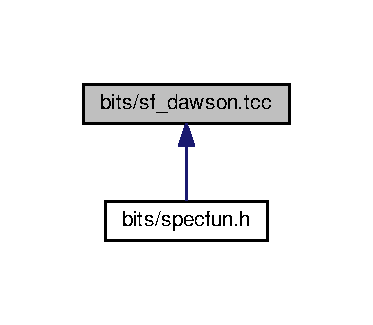
\includegraphics[width=179pt]{sf__dawson_8tcc__dep__incl}
\end{center}
\end{figure}
\subsection*{Namespaces}
\begin{DoxyCompactItemize}
\item 
 \hyperlink{namespacestd}{std}
\item 
 \hyperlink{namespacestd_1_1____detail}{std\+::\+\_\+\+\_\+detail}
\end{DoxyCompactItemize}
\subsection*{Macros}
\begin{DoxyCompactItemize}
\item 
\#define \hyperlink{sf__dawson_8tcc_a72d0ce5cd51240da4fb2546e640923de}{\+\_\+\+G\+L\+I\+B\+C\+X\+X\+\_\+\+S\+F\+\_\+\+D\+A\+W\+S\+O\+N\+\_\+\+T\+C\+C}~1
\end{DoxyCompactItemize}
\subsection*{Functions}
\begin{DoxyCompactItemize}
\item 
{\footnotesize template$<$typename \+\_\+\+Tp $>$ }\\\+\_\+\+Tp \hyperlink{namespacestd_1_1____detail_a6384fb4c5af31b41a38c120869a548c7}{std\+::\+\_\+\+\_\+detail\+::\+\_\+\+\_\+dawson} (\+\_\+\+Tp \+\_\+\+\_\+x)
\begin{DoxyCompactList}\small\item\em Return the Dawson integral, $ F(x) $, for real argument {\ttfamily x}. \end{DoxyCompactList}\item 
{\footnotesize template$<$typename \+\_\+\+Tp $>$ }\\\+\_\+\+Tp \hyperlink{namespacestd_1_1____detail_a3fe9fa143beb1a5d9f8ca18b3783f650}{std\+::\+\_\+\+\_\+detail\+::\+\_\+\+\_\+dawson\+\_\+const\+\_\+frac} (\+\_\+\+Tp \+\_\+\+\_\+x)
\begin{DoxyCompactList}\small\item\em Compute the Dawson integral using a sampling theorem representation. \end{DoxyCompactList}\item 
{\footnotesize template$<$typename \+\_\+\+Tp $>$ }\\\+\_\+\+Tp \hyperlink{namespacestd_1_1____detail_a033d91cc1c67280385ff3d1d809a21d1}{std\+::\+\_\+\+\_\+detail\+::\+\_\+\+\_\+dawson\+\_\+series} (\+\_\+\+Tp \+\_\+\+\_\+x)
\begin{DoxyCompactList}\small\item\em Compute the Dawson integral using the series expansion. \end{DoxyCompactList}\end{DoxyCompactItemize}


\subsection{Detailed Description}
This is an internal header file, included by other library headers. Do not attempt to use it directly. Instead, include $<$cmath$>$. 

\subsection{Macro Definition Documentation}
\hypertarget{sf__dawson_8tcc_a72d0ce5cd51240da4fb2546e640923de}{}\index{sf\+\_\+dawson.\+tcc@{sf\+\_\+dawson.\+tcc}!\+\_\+\+G\+L\+I\+B\+C\+X\+X\+\_\+\+S\+F\+\_\+\+D\+A\+W\+S\+O\+N\+\_\+\+T\+C\+C@{\+\_\+\+G\+L\+I\+B\+C\+X\+X\+\_\+\+S\+F\+\_\+\+D\+A\+W\+S\+O\+N\+\_\+\+T\+C\+C}}
\index{\+\_\+\+G\+L\+I\+B\+C\+X\+X\+\_\+\+S\+F\+\_\+\+D\+A\+W\+S\+O\+N\+\_\+\+T\+C\+C@{\+\_\+\+G\+L\+I\+B\+C\+X\+X\+\_\+\+S\+F\+\_\+\+D\+A\+W\+S\+O\+N\+\_\+\+T\+C\+C}!sf\+\_\+dawson.\+tcc@{sf\+\_\+dawson.\+tcc}}
\subsubsection[{\+\_\+\+G\+L\+I\+B\+C\+X\+X\+\_\+\+S\+F\+\_\+\+D\+A\+W\+S\+O\+N\+\_\+\+T\+C\+C}]{\setlength{\rightskip}{0pt plus 5cm}\#define \+\_\+\+G\+L\+I\+B\+C\+X\+X\+\_\+\+S\+F\+\_\+\+D\+A\+W\+S\+O\+N\+\_\+\+T\+C\+C~1}\label{sf__dawson_8tcc_a72d0ce5cd51240da4fb2546e640923de}


Definition at line 31 of file sf\+\_\+dawson.\+tcc.


\hypertarget{sf__distributions_8tcc}{}\section{bits/sf\+\_\+distributions.tcc File Reference}
\label{sf__distributions_8tcc}\index{bits/sf\+\_\+distributions.\+tcc@{bits/sf\+\_\+distributions.\+tcc}}
{\ttfamily \#include $<$ext/math\+\_\+const.\+h$>$}\newline
Include dependency graph for sf\+\_\+distributions.\+tcc\+:
\nopagebreak
\begin{figure}[H]
\begin{center}
\leavevmode
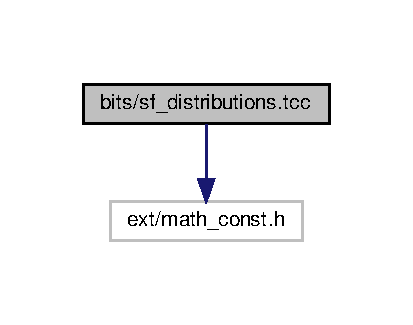
\includegraphics[width=198pt]{sf__distributions_8tcc__incl}
\end{center}
\end{figure}
This graph shows which files directly or indirectly include this file\+:
\nopagebreak
\begin{figure}[H]
\begin{center}
\leavevmode
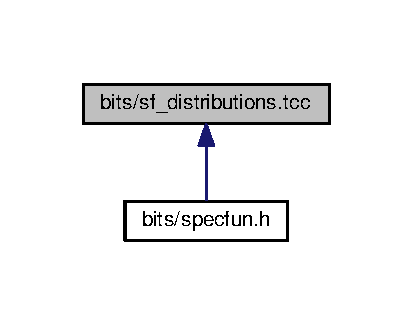
\includegraphics[width=198pt]{sf__distributions_8tcc__dep__incl}
\end{center}
\end{figure}
\subsection*{Namespaces}
\begin{DoxyCompactItemize}
\item 
 \hyperlink{namespacestd}{std}
\item 
 \hyperlink{namespacestd_1_1____detail}{std\+::\+\_\+\+\_\+detail}
\end{DoxyCompactItemize}
\subsection*{Macros}
\begin{DoxyCompactItemize}
\item 
\#define \hyperlink{sf__distributions_8tcc_a3af0d272d6bbb6104b89109f772d6092}{\+\_\+\+G\+L\+I\+B\+C\+X\+X\+\_\+\+B\+I\+T\+S\+\_\+\+S\+F\+\_\+\+D\+I\+S\+T\+R\+I\+B\+U\+T\+I\+O\+N\+S\+\_\+\+T\+CC}~1
\end{DoxyCompactItemize}
\subsection*{Functions}
\begin{DoxyCompactItemize}
\item 
{\footnotesize template$<$typename \+\_\+\+Tp $>$ }\\\+\_\+\+Tp \hyperlink{namespacestd_1_1____detail_aefa3217863e0f50cd8f5379947cefcbd}{std\+::\+\_\+\+\_\+detail\+::\+\_\+\+\_\+binomial\+\_\+cdf} (\+\_\+\+Tp \+\_\+\+\_\+p, unsigned int \+\_\+\+\_\+n, unsigned int \+\_\+\+\_\+k)
\begin{DoxyCompactList}\small\item\em Return the binomial cumulative distribution function. \end{DoxyCompactList}\item 
{\footnotesize template$<$typename \+\_\+\+Tp $>$ }\\\+\_\+\+Tp \hyperlink{namespacestd_1_1____detail_a1fd732a432f73686c97311e6976a0e76}{std\+::\+\_\+\+\_\+detail\+::\+\_\+\+\_\+binomial\+\_\+cdfc} (\+\_\+\+Tp \+\_\+\+\_\+p, unsigned int \+\_\+\+\_\+n, unsigned int \+\_\+\+\_\+k)
\begin{DoxyCompactList}\small\item\em Return the complementary binomial cumulative distribution function. \end{DoxyCompactList}\item 
{\footnotesize template$<$typename \+\_\+\+Tp $>$ }\\\+\_\+\+Tp \hyperlink{namespacestd_1_1____detail_acaeb596397431731cba684ca1f04cbfc}{std\+::\+\_\+\+\_\+detail\+::\+\_\+\+\_\+binomial\+\_\+pdf} (\+\_\+\+Tp \+\_\+\+\_\+p, unsigned int \+\_\+\+\_\+n, unsigned int \+\_\+\+\_\+k)
\begin{DoxyCompactList}\small\item\em Return the binomial probability mass function. \end{DoxyCompactList}\item 
{\footnotesize template$<$typename \+\_\+\+Tp $>$ }\\\+\_\+\+Tp \hyperlink{namespacestd_1_1____detail_a2125cbbc3fd3aad11c8025478c7a14fe}{std\+::\+\_\+\+\_\+detail\+::\+\_\+\+\_\+chi\+\_\+squared\+\_\+pdf} (\+\_\+\+Tp \+\_\+\+\_\+chi2, unsigned int \+\_\+\+\_\+nu)
\begin{DoxyCompactList}\small\item\em Return the chi-\/squared propability function. This returns the probability that the observed chi-\/squared for a correct model is less than the value $ \chi^2 $. \end{DoxyCompactList}\item 
{\footnotesize template$<$typename \+\_\+\+Tp $>$ }\\\+\_\+\+Tp \hyperlink{namespacestd_1_1____detail_aa62c16dd75a7411400c7082e6b2b246b}{std\+::\+\_\+\+\_\+detail\+::\+\_\+\+\_\+chi\+\_\+squared\+\_\+pdfc} (\+\_\+\+Tp \+\_\+\+\_\+chi2, unsigned int \+\_\+\+\_\+nu)
\begin{DoxyCompactList}\small\item\em Return the complementary chi-\/squared propability function. This returns the probability that the observed chi-\/squared for a correct model is greater than the value $ \chi^2 $. \end{DoxyCompactList}\item 
{\footnotesize template$<$typename \+\_\+\+Tp $>$ }\\\+\_\+\+Tp \hyperlink{namespacestd_1_1____detail_ada7f806f891a02d7825ec9a8862302ad}{std\+::\+\_\+\+\_\+detail\+::\+\_\+\+\_\+exponential\+\_\+cdf} (\+\_\+\+Tp \+\_\+\+\_\+lambda, \+\_\+\+Tp \+\_\+\+\_\+x)
\begin{DoxyCompactList}\small\item\em Return the exponential cumulative probability density function. \end{DoxyCompactList}\item 
{\footnotesize template$<$typename \+\_\+\+Tp $>$ }\\\+\_\+\+Tp \hyperlink{namespacestd_1_1____detail_a4e72483dfbfe8c866974d89f9aeb4b28}{std\+::\+\_\+\+\_\+detail\+::\+\_\+\+\_\+exponential\+\_\+cdfc} (\+\_\+\+Tp \+\_\+\+\_\+lambda, \+\_\+\+Tp \+\_\+\+\_\+x)
\begin{DoxyCompactList}\small\item\em Return the complement of the exponential cumulative probability density function. \end{DoxyCompactList}\item 
{\footnotesize template$<$typename \+\_\+\+Tp $>$ }\\\+\_\+\+Tp \hyperlink{namespacestd_1_1____detail_add35fd0c4c00f412c0fab7b6018ce2cd}{std\+::\+\_\+\+\_\+detail\+::\+\_\+\+\_\+exponential\+\_\+pdf} (\+\_\+\+Tp \+\_\+\+\_\+lambda, \+\_\+\+Tp \+\_\+\+\_\+x)
\begin{DoxyCompactList}\small\item\em Return the exponential probability density function. \end{DoxyCompactList}\item 
{\footnotesize template$<$typename \+\_\+\+Tp $>$ }\\\+\_\+\+Tp \hyperlink{namespacestd_1_1____detail_a3825f4b63cdd255c1ca790bf16d844a1}{std\+::\+\_\+\+\_\+detail\+::\+\_\+\+\_\+fisher\+\_\+f\+\_\+cdf} (\+\_\+\+Tp \+\_\+\+\_\+F, unsigned int \+\_\+\+\_\+nu1, unsigned int \+\_\+\+\_\+nu2)
\begin{DoxyCompactList}\small\item\em Return the F-\/distribution propability function. This returns the probability that the observed chi-\/square for a correct model exceeds the value $ \chi^2 $. \end{DoxyCompactList}\item 
{\footnotesize template$<$typename \+\_\+\+Tp $>$ }\\\+\_\+\+Tp \hyperlink{namespacestd_1_1____detail_ae02418cde6461a9e65f926c974c216a2}{std\+::\+\_\+\+\_\+detail\+::\+\_\+\+\_\+fisher\+\_\+f\+\_\+cdfc} (\+\_\+\+Tp \+\_\+\+\_\+F, unsigned int \+\_\+\+\_\+nu1, unsigned int \+\_\+\+\_\+nu2)
\begin{DoxyCompactList}\small\item\em Return the F-\/distribution propability function. This returns the probability that the observed chi-\/square for a correct model exceeds the value $ \chi^2 $. \end{DoxyCompactList}\item 
{\footnotesize template$<$typename \+\_\+\+Tp $>$ }\\\+\_\+\+Tp \hyperlink{namespacestd_1_1____detail_a2f85415264800034e969f86ac8294f7b}{std\+::\+\_\+\+\_\+detail\+::\+\_\+\+\_\+fisher\+\_\+f\+\_\+pdf} (\+\_\+\+Tp \+\_\+\+\_\+F, unsigned int \+\_\+\+\_\+nu1, unsigned int \+\_\+\+\_\+nu2)
\begin{DoxyCompactList}\small\item\em Return the F-\/distribution propability function. This returns the probability that the observed chi-\/square for a correct model exceeds the value $ \chi^2 $. \end{DoxyCompactList}\item 
{\footnotesize template$<$typename \+\_\+\+Tp $>$ }\\\+\_\+\+Tp \hyperlink{namespacestd_1_1____detail_aa4f1cd082a56f66b7ac2f8d805f66a81}{std\+::\+\_\+\+\_\+detail\+::\+\_\+\+\_\+gamma\+\_\+cdf} (\+\_\+\+Tp \+\_\+\+\_\+alpha, \+\_\+\+Tp \+\_\+\+\_\+beta, \+\_\+\+Tp \+\_\+\+\_\+x)
\begin{DoxyCompactList}\small\item\em Return the gamma cumulative propability distribution function. \end{DoxyCompactList}\item 
{\footnotesize template$<$typename \+\_\+\+Tp $>$ }\\\+\_\+\+Tp \hyperlink{namespacestd_1_1____detail_a7dc59114c8c223b5570c374a7192d404}{std\+::\+\_\+\+\_\+detail\+::\+\_\+\+\_\+gamma\+\_\+cdfc} (\+\_\+\+Tp \+\_\+\+\_\+alpha, \+\_\+\+Tp \+\_\+\+\_\+beta, \+\_\+\+Tp \+\_\+\+\_\+x)
\begin{DoxyCompactList}\small\item\em Return the gamma complementary cumulative propability distribution function. \end{DoxyCompactList}\item 
{\footnotesize template$<$typename \+\_\+\+Tp $>$ }\\\+\_\+\+Tp \hyperlink{namespacestd_1_1____detail_a13146321e4e094815de990c33b83b02a}{std\+::\+\_\+\+\_\+detail\+::\+\_\+\+\_\+gamma\+\_\+pdf} (\+\_\+\+Tp \+\_\+\+\_\+alpha, \+\_\+\+Tp \+\_\+\+\_\+beta, \+\_\+\+Tp \+\_\+\+\_\+x)
\begin{DoxyCompactList}\small\item\em Return the gamma propability distribution function. \end{DoxyCompactList}\item 
{\footnotesize template$<$typename \+\_\+\+Tp $>$ }\\\+\_\+\+Tp \hyperlink{namespacestd_1_1____detail_abe893340d3de850ff3c9701deb914f96}{std\+::\+\_\+\+\_\+detail\+::\+\_\+\+\_\+logistic\+\_\+cdf} (\+\_\+\+Tp \+\_\+\+\_\+a, \+\_\+\+Tp \+\_\+\+\_\+b, \+\_\+\+Tp \+\_\+\+\_\+x)
\begin{DoxyCompactList}\small\item\em Return the logistic cumulative distribution function. \end{DoxyCompactList}\item 
{\footnotesize template$<$typename \+\_\+\+Tp $>$ }\\\+\_\+\+Tp \hyperlink{namespacestd_1_1____detail_a4c845b9f17fc3e35dccc0954d82d62f9}{std\+::\+\_\+\+\_\+detail\+::\+\_\+\+\_\+logistic\+\_\+pdf} (\+\_\+\+Tp \+\_\+\+\_\+a, \+\_\+\+Tp \+\_\+\+\_\+b, \+\_\+\+Tp \+\_\+\+\_\+x)
\begin{DoxyCompactList}\small\item\em Return the logistic probability density function. \end{DoxyCompactList}\item 
{\footnotesize template$<$typename \+\_\+\+Tp $>$ }\\\+\_\+\+Tp \hyperlink{namespacestd_1_1____detail_a871cf2e541cc4f8a79e4d219c628edc4}{std\+::\+\_\+\+\_\+detail\+::\+\_\+\+\_\+lognormal\+\_\+cdf} (\+\_\+\+Tp \+\_\+\+\_\+mu, \+\_\+\+Tp \+\_\+\+\_\+sigma, \+\_\+\+Tp \+\_\+\+\_\+x)
\begin{DoxyCompactList}\small\item\em Return the lognormal cumulative probability density function. \end{DoxyCompactList}\item 
{\footnotesize template$<$typename \+\_\+\+Tp $>$ }\\\+\_\+\+Tp \hyperlink{namespacestd_1_1____detail_a46c5dea7a38f38965bce5a84d389a02b}{std\+::\+\_\+\+\_\+detail\+::\+\_\+\+\_\+lognormal\+\_\+pdf} (\+\_\+\+Tp \+\_\+\+\_\+nu, \+\_\+\+Tp \+\_\+\+\_\+sigma, \+\_\+\+Tp \+\_\+\+\_\+x)
\begin{DoxyCompactList}\small\item\em Return the lognormal probability density function. \end{DoxyCompactList}\item 
{\footnotesize template$<$typename \+\_\+\+Tp $>$ }\\\+\_\+\+Tp \hyperlink{namespacestd_1_1____detail_a718b0f0884f0bc91b038ef4dabbb7427}{std\+::\+\_\+\+\_\+detail\+::\+\_\+\+\_\+normal\+\_\+cdf} (\+\_\+\+Tp \+\_\+\+\_\+mu, \+\_\+\+Tp \+\_\+\+\_\+sigma, \+\_\+\+Tp \+\_\+\+\_\+x)
\begin{DoxyCompactList}\small\item\em Return the normal cumulative probability density function. \end{DoxyCompactList}\item 
{\footnotesize template$<$typename \+\_\+\+Tp $>$ }\\\+\_\+\+Tp \hyperlink{namespacestd_1_1____detail_a6211a0741c8e2dfb219fb52d072295f4}{std\+::\+\_\+\+\_\+detail\+::\+\_\+\+\_\+normal\+\_\+pdf} (\+\_\+\+Tp \+\_\+\+\_\+mu, \+\_\+\+Tp \+\_\+\+\_\+sigma, \+\_\+\+Tp \+\_\+\+\_\+x)
\begin{DoxyCompactList}\small\item\em Return the normal probability density function. \end{DoxyCompactList}\item 
{\footnotesize template$<$typename \+\_\+\+Tp $>$ }\\\+\_\+\+Tp \hyperlink{namespacestd_1_1____detail_a571f37fdf793a91985073a58a873e731}{std\+::\+\_\+\+\_\+detail\+::\+\_\+\+\_\+rice\+\_\+pdf} (\+\_\+\+Tp \+\_\+\+\_\+nu, \+\_\+\+Tp \+\_\+\+\_\+sigma, \+\_\+\+Tp \+\_\+\+\_\+x)
\begin{DoxyCompactList}\small\item\em Return the Rice probability density function. \end{DoxyCompactList}\item 
{\footnotesize template$<$typename \+\_\+\+Tp $>$ }\\\+\_\+\+Tp \hyperlink{namespacestd_1_1____detail_aadc19f2a38494343a752a8d4f924e3df}{std\+::\+\_\+\+\_\+detail\+::\+\_\+\+\_\+student\+\_\+t\+\_\+cdf} (\+\_\+\+Tp \+\_\+\+\_\+t, unsigned int \+\_\+\+\_\+nu)
\begin{DoxyCompactList}\small\item\em Return the Students T probability function. \end{DoxyCompactList}\item 
{\footnotesize template$<$typename \+\_\+\+Tp $>$ }\\\+\_\+\+Tp \hyperlink{namespacestd_1_1____detail_a3009eaaa4b7d6d845878765ef0e3fa27}{std\+::\+\_\+\+\_\+detail\+::\+\_\+\+\_\+student\+\_\+t\+\_\+cdfc} (\+\_\+\+Tp \+\_\+\+\_\+t, unsigned int \+\_\+\+\_\+nu)
\begin{DoxyCompactList}\small\item\em Return the complement of the Students T probability function. \end{DoxyCompactList}\item 
{\footnotesize template$<$typename \+\_\+\+Tp $>$ }\\\+\_\+\+Tp \hyperlink{namespacestd_1_1____detail_a866bf8f03fd2d5de5024837727beecd8}{std\+::\+\_\+\+\_\+detail\+::\+\_\+\+\_\+student\+\_\+t\+\_\+pdf} (\+\_\+\+Tp \+\_\+\+\_\+t, unsigned int \+\_\+\+\_\+nu)
\begin{DoxyCompactList}\small\item\em Return the Students T probability density. \end{DoxyCompactList}\item 
{\footnotesize template$<$typename \+\_\+\+Tp $>$ }\\\+\_\+\+Tp \hyperlink{namespacestd_1_1____detail_aeb9a99b7ca44c9e403f78baf38dc293b}{std\+::\+\_\+\+\_\+detail\+::\+\_\+\+\_\+weibull\+\_\+cdf} (\+\_\+\+Tp \+\_\+\+\_\+a, \+\_\+\+Tp \+\_\+\+\_\+b, \+\_\+\+Tp \+\_\+\+\_\+x)
\begin{DoxyCompactList}\small\item\em Return the Weibull cumulative probability density function. \end{DoxyCompactList}\item 
{\footnotesize template$<$typename \+\_\+\+Tp $>$ }\\\+\_\+\+Tp \hyperlink{namespacestd_1_1____detail_ab15a21521bc750303938a108c5a0bb0b}{std\+::\+\_\+\+\_\+detail\+::\+\_\+\+\_\+weibull\+\_\+pdf} (\+\_\+\+Tp \+\_\+\+\_\+a, \+\_\+\+Tp \+\_\+\+\_\+b, \+\_\+\+Tp \+\_\+\+\_\+x)
\begin{DoxyCompactList}\small\item\em Return the Weibull probability density function. \end{DoxyCompactList}\end{DoxyCompactItemize}


\subsection{Detailed Description}
This is an internal header file, included by other library headers. Do not attempt to use it directly. Instead, include $<$cmath$>$. 

\subsection{Macro Definition Documentation}
\mbox{\Hypertarget{sf__distributions_8tcc_a3af0d272d6bbb6104b89109f772d6092}\label{sf__distributions_8tcc_a3af0d272d6bbb6104b89109f772d6092}} 
\index{sf\+\_\+distributions.\+tcc@{sf\+\_\+distributions.\+tcc}!\+\_\+\+G\+L\+I\+B\+C\+X\+X\+\_\+\+B\+I\+T\+S\+\_\+\+S\+F\+\_\+\+D\+I\+S\+T\+R\+I\+B\+U\+T\+I\+O\+N\+S\+\_\+\+T\+CC@{\+\_\+\+G\+L\+I\+B\+C\+X\+X\+\_\+\+B\+I\+T\+S\+\_\+\+S\+F\+\_\+\+D\+I\+S\+T\+R\+I\+B\+U\+T\+I\+O\+N\+S\+\_\+\+T\+CC}}
\index{\+\_\+\+G\+L\+I\+B\+C\+X\+X\+\_\+\+B\+I\+T\+S\+\_\+\+S\+F\+\_\+\+D\+I\+S\+T\+R\+I\+B\+U\+T\+I\+O\+N\+S\+\_\+\+T\+CC@{\+\_\+\+G\+L\+I\+B\+C\+X\+X\+\_\+\+B\+I\+T\+S\+\_\+\+S\+F\+\_\+\+D\+I\+S\+T\+R\+I\+B\+U\+T\+I\+O\+N\+S\+\_\+\+T\+CC}!sf\+\_\+distributions.\+tcc@{sf\+\_\+distributions.\+tcc}}
\subsubsection{\texorpdfstring{\+\_\+\+G\+L\+I\+B\+C\+X\+X\+\_\+\+B\+I\+T\+S\+\_\+\+S\+F\+\_\+\+D\+I\+S\+T\+R\+I\+B\+U\+T\+I\+O\+N\+S\+\_\+\+T\+CC}{\_GLIBCXX\_BITS\_SF\_DISTRIBUTIONS\_TCC}}
{\footnotesize\ttfamily \#define \+\_\+\+G\+L\+I\+B\+C\+X\+X\+\_\+\+B\+I\+T\+S\+\_\+\+S\+F\+\_\+\+D\+I\+S\+T\+R\+I\+B\+U\+T\+I\+O\+N\+S\+\_\+\+T\+CC~1}



Definition at line 49 of file sf\+\_\+distributions.\+tcc.


\hypertarget{sf__ellint_8tcc}{}\section{sf\+\_\+ellint.\+tcc File Reference}
\label{sf__ellint_8tcc}\index{sf\+\_\+ellint.\+tcc@{sf\+\_\+ellint.\+tcc}}
{\ttfamily \#include $<$ext/math\+\_\+const.\+h$>$}\\*
Include dependency graph for sf\+\_\+ellint.\+tcc\+:
\nopagebreak
\begin{figure}[H]
\begin{center}
\leavevmode
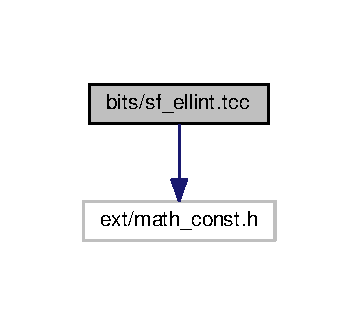
\includegraphics[width=172pt]{sf__ellint_8tcc__incl}
\end{center}
\end{figure}
\subsection*{Namespaces}
\begin{DoxyCompactItemize}
\item 
 \hyperlink{namespacestd}{std}
\item 
 \hyperlink{namespacestd_1_1____detail}{std\+::\+\_\+\+\_\+detail}
\end{DoxyCompactItemize}
\subsection*{Macros}
\begin{DoxyCompactItemize}
\item 
\#define \hyperlink{sf__ellint_8tcc_a4b6f21b1d48bfb7a988fe3346437ccce}{\+\_\+\+G\+L\+I\+B\+C\+X\+X\+\_\+\+B\+I\+T\+S\+\_\+\+S\+F\+\_\+\+E\+L\+L\+I\+N\+T\+\_\+\+T\+C\+C}~1
\end{DoxyCompactItemize}
\subsection*{Functions}
\begin{DoxyCompactItemize}
\item 
{\footnotesize template$<$typename \+\_\+\+Tp $>$ }\\\+\_\+\+Tp \hyperlink{namespacestd_1_1____detail_a7b23bcf7e9f20b1e353a047126e13af1}{std\+::\+\_\+\+\_\+detail\+::\+\_\+\+\_\+comp\+\_\+ellint\+\_\+1} (\+\_\+\+Tp \+\_\+\+\_\+k)
\begin{DoxyCompactList}\small\item\em Return the complete elliptic integral of the first kind $ K(k) $ using the Carlson formulation. \end{DoxyCompactList}\item 
{\footnotesize template$<$typename \+\_\+\+Tp $>$ }\\\+\_\+\+Tp \hyperlink{namespacestd_1_1____detail_a4836f4db24abd037705100750f82d375}{std\+::\+\_\+\+\_\+detail\+::\+\_\+\+\_\+comp\+\_\+ellint\+\_\+2} (\+\_\+\+Tp \+\_\+\+\_\+k)
\begin{DoxyCompactList}\small\item\em Return the complete elliptic integral of the second kind $ E(k) $ using the Carlson formulation. \end{DoxyCompactList}\item 
{\footnotesize template$<$typename \+\_\+\+Tp $>$ }\\\+\_\+\+Tp \hyperlink{namespacestd_1_1____detail_a26b35b5d72366d30ac4644db8f2f8be4}{std\+::\+\_\+\+\_\+detail\+::\+\_\+\+\_\+comp\+\_\+ellint\+\_\+3} (\+\_\+\+Tp \+\_\+\+\_\+k, \+\_\+\+Tp \+\_\+\+\_\+nu)
\begin{DoxyCompactList}\small\item\em Return the complete elliptic integral of the third kind $ \Pi(k,\nu) = \Pi(k,\nu,\pi/2) $ using the Carlson formulation. \end{DoxyCompactList}\item 
{\footnotesize template$<$typename \+\_\+\+Tp $>$ }\\\+\_\+\+Tp \hyperlink{namespacestd_1_1____detail_add5220a1ab03915e4a45dc547bb8eef6}{std\+::\+\_\+\+\_\+detail\+::\+\_\+\+\_\+comp\+\_\+ellint\+\_\+d} (\+\_\+\+Tp \+\_\+\+\_\+k)
\item 
{\footnotesize template$<$typename \+\_\+\+Tp $>$ }\\\+\_\+\+Tp \hyperlink{namespacestd_1_1____detail_a41ecec8820344d3575b464ecd4db5171}{std\+::\+\_\+\+\_\+detail\+::\+\_\+\+\_\+comp\+\_\+ellint\+\_\+rf} (\+\_\+\+Tp \+\_\+\+\_\+x, \+\_\+\+Tp \+\_\+\+\_\+y)
\item 
{\footnotesize template$<$typename \+\_\+\+Tp $>$ }\\\+\_\+\+Tp \hyperlink{namespacestd_1_1____detail_a31bb5a6e359c88b5bece8dd73f76a2f9}{std\+::\+\_\+\+\_\+detail\+::\+\_\+\+\_\+comp\+\_\+ellint\+\_\+rg} (\+\_\+\+Tp \+\_\+\+\_\+x, \+\_\+\+Tp \+\_\+\+\_\+y)
\item 
{\footnotesize template$<$typename \+\_\+\+Tp $>$ }\\\+\_\+\+Tp \hyperlink{namespacestd_1_1____detail_aa349fe5bcf36d29cfacf6cd3e8aa65b0}{std\+::\+\_\+\+\_\+detail\+::\+\_\+\+\_\+ellint\+\_\+1} (\+\_\+\+Tp \+\_\+\+\_\+k, \+\_\+\+Tp \+\_\+\+\_\+phi)
\begin{DoxyCompactList}\small\item\em Return the incomplete elliptic integral of the first kind $ F(k,\phi) $ using the Carlson formulation. \end{DoxyCompactList}\item 
{\footnotesize template$<$typename \+\_\+\+Tp $>$ }\\\+\_\+\+Tp \hyperlink{namespacestd_1_1____detail_ad3687a38e74e5fbf08265501add0b56a}{std\+::\+\_\+\+\_\+detail\+::\+\_\+\+\_\+ellint\+\_\+2} (\+\_\+\+Tp \+\_\+\+\_\+k, \+\_\+\+Tp \+\_\+\+\_\+phi)
\begin{DoxyCompactList}\small\item\em Return the incomplete elliptic integral of the second kind $ E(k,\phi) $ using the Carlson formulation. \end{DoxyCompactList}\item 
{\footnotesize template$<$typename \+\_\+\+Tp $>$ }\\\+\_\+\+Tp \hyperlink{namespacestd_1_1____detail_a9c6ea96cd5d6907fce278010b992499a}{std\+::\+\_\+\+\_\+detail\+::\+\_\+\+\_\+ellint\+\_\+3} (\+\_\+\+Tp \+\_\+\+\_\+k, \+\_\+\+Tp \+\_\+\+\_\+nu, \+\_\+\+Tp \+\_\+\+\_\+phi)
\begin{DoxyCompactList}\small\item\em Return the incomplete elliptic integral of the third kind $ \Pi(k,\nu,\phi) $ using the Carlson formulation. \end{DoxyCompactList}\item 
{\footnotesize template$<$typename \+\_\+\+Tp $>$ }\\\+\_\+\+Tp \hyperlink{namespacestd_1_1____detail_a7c7d04715f0d40e054299312db35e32d}{std\+::\+\_\+\+\_\+detail\+::\+\_\+\+\_\+ellint\+\_\+cel} (\+\_\+\+Tp \+\_\+\+\_\+k\+\_\+c, \+\_\+\+Tp \+\_\+\+\_\+p, \+\_\+\+Tp \+\_\+\+\_\+a, \+\_\+\+Tp \+\_\+\+\_\+b)
\item 
{\footnotesize template$<$typename \+\_\+\+Tp $>$ }\\\+\_\+\+Tp \hyperlink{namespacestd_1_1____detail_a00da42d89830fd51e9934fe0c5e08b7f}{std\+::\+\_\+\+\_\+detail\+::\+\_\+\+\_\+ellint\+\_\+d} (\+\_\+\+Tp \+\_\+\+\_\+k, \+\_\+\+Tp \+\_\+\+\_\+phi)
\item 
{\footnotesize template$<$typename \+\_\+\+Tp $>$ }\\\+\_\+\+Tp \hyperlink{namespacestd_1_1____detail_aa17b1b382a89552f49fbb8c5eda1d50f}{std\+::\+\_\+\+\_\+detail\+::\+\_\+\+\_\+ellint\+\_\+el1} (\+\_\+\+Tp \+\_\+\+\_\+x, \+\_\+\+Tp \+\_\+\+\_\+k\+\_\+c)
\item 
{\footnotesize template$<$typename \+\_\+\+Tp $>$ }\\\+\_\+\+Tp \hyperlink{namespacestd_1_1____detail_a82449d0f05d40ba2cef6b8fc57dd5bae}{std\+::\+\_\+\+\_\+detail\+::\+\_\+\+\_\+ellint\+\_\+el2} (\+\_\+\+Tp \+\_\+\+\_\+x, \+\_\+\+Tp \+\_\+\+\_\+k\+\_\+c, \+\_\+\+Tp \+\_\+\+\_\+a, \+\_\+\+Tp \+\_\+\+\_\+b)
\item 
{\footnotesize template$<$typename \+\_\+\+Tp $>$ }\\\+\_\+\+Tp \hyperlink{namespacestd_1_1____detail_a2a2b5b80edd39b3d1f852f10c5f277fc}{std\+::\+\_\+\+\_\+detail\+::\+\_\+\+\_\+ellint\+\_\+el3} (\+\_\+\+Tp \+\_\+\+\_\+x, \+\_\+\+Tp \+\_\+\+\_\+k\+\_\+c, \+\_\+\+Tp \+\_\+\+\_\+p)
\item 
{\footnotesize template$<$typename \+\_\+\+Tp $>$ }\\\+\_\+\+Tp \hyperlink{namespacestd_1_1____detail_aa7d81e41240a6d031414c6b117889e36}{std\+::\+\_\+\+\_\+detail\+::\+\_\+\+\_\+ellint\+\_\+rc} (\+\_\+\+Tp \+\_\+\+\_\+x, \+\_\+\+Tp \+\_\+\+\_\+y)
\begin{DoxyCompactList}\small\item\em Return the Carlson elliptic function $ R_C(x,y) = R_F(x,y,y) $ where $ R_F(x,y,z) $ is the Carlson elliptic function of the first kind. \end{DoxyCompactList}\item 
{\footnotesize template$<$typename \+\_\+\+Tp $>$ }\\\+\_\+\+Tp \hyperlink{namespacestd_1_1____detail_ac05883415a662fc6f9855dd8d1da921f}{std\+::\+\_\+\+\_\+detail\+::\+\_\+\+\_\+ellint\+\_\+rd} (\+\_\+\+Tp \+\_\+\+\_\+x, \+\_\+\+Tp \+\_\+\+\_\+y, \+\_\+\+Tp \+\_\+\+\_\+z)
\begin{DoxyCompactList}\small\item\em Return the Carlson elliptic function of the second kind $ R_D(x,y,z) = R_J(x,y,z,z) $ where $ R_J(x,y,z,p) $ is the Carlson elliptic function of the third kind. \end{DoxyCompactList}\item 
{\footnotesize template$<$typename \+\_\+\+Tp $>$ }\\\+\_\+\+Tp \hyperlink{namespacestd_1_1____detail_a2cca271dcbdf22923219eab7a02450d5}{std\+::\+\_\+\+\_\+detail\+::\+\_\+\+\_\+ellint\+\_\+rf} (\+\_\+\+Tp \+\_\+\+\_\+x, \+\_\+\+Tp \+\_\+\+\_\+y, \+\_\+\+Tp \+\_\+\+\_\+z)
\begin{DoxyCompactList}\small\item\em Return the Carlson elliptic function $ R_F(x,y,z) $ of the first kind. \end{DoxyCompactList}\item 
{\footnotesize template$<$typename \+\_\+\+Tp $>$ }\\\+\_\+\+Tp \hyperlink{namespacestd_1_1____detail_aaceff1eb320e0602afee36c60b80f87a}{std\+::\+\_\+\+\_\+detail\+::\+\_\+\+\_\+ellint\+\_\+rg} (\+\_\+\+Tp \+\_\+\+\_\+x, \+\_\+\+Tp \+\_\+\+\_\+y, \+\_\+\+Tp \+\_\+\+\_\+z)
\begin{DoxyCompactList}\small\item\em Return the symmetric Carlson elliptic function of the second kind $ R_G(x,y,z) $. \end{DoxyCompactList}\item 
{\footnotesize template$<$typename \+\_\+\+Tp $>$ }\\\+\_\+\+Tp \hyperlink{namespacestd_1_1____detail_afe05ce66130b5f47389137c3f9aa6949}{std\+::\+\_\+\+\_\+detail\+::\+\_\+\+\_\+ellint\+\_\+rj} (\+\_\+\+Tp \+\_\+\+\_\+x, \+\_\+\+Tp \+\_\+\+\_\+y, \+\_\+\+Tp \+\_\+\+\_\+z, \+\_\+\+Tp \+\_\+\+\_\+p)
\begin{DoxyCompactList}\small\item\em Return the Carlson elliptic function $ R_J(x,y,z,p) $ of the third kind. \end{DoxyCompactList}\item 
{\footnotesize template$<$typename \+\_\+\+Tp $>$ }\\\+\_\+\+Tp \hyperlink{namespacestd_1_1____detail_a90938823a16cabc06031ebf209066a94}{std\+::\+\_\+\+\_\+detail\+::\+\_\+\+\_\+heuman\+\_\+lambda} (\+\_\+\+Tp \+\_\+\+\_\+k, \+\_\+\+Tp \+\_\+\+\_\+phi)
\item 
{\footnotesize template$<$typename \+\_\+\+Tp $>$ }\\\+\_\+\+Tp \hyperlink{namespacestd_1_1____detail_a1d5fc69202703d72974c4370fd7ade03}{std\+::\+\_\+\+\_\+detail\+::\+\_\+\+\_\+jacobi\+\_\+zeta} (\+\_\+\+Tp \+\_\+\+\_\+k, \+\_\+\+Tp \+\_\+\+\_\+phi)
\end{DoxyCompactItemize}


\subsection{Macro Definition Documentation}
\hypertarget{sf__ellint_8tcc_a4b6f21b1d48bfb7a988fe3346437ccce}{}\index{sf\+\_\+ellint.\+tcc@{sf\+\_\+ellint.\+tcc}!\+\_\+\+G\+L\+I\+B\+C\+X\+X\+\_\+\+B\+I\+T\+S\+\_\+\+S\+F\+\_\+\+E\+L\+L\+I\+N\+T\+\_\+\+T\+C\+C@{\+\_\+\+G\+L\+I\+B\+C\+X\+X\+\_\+\+B\+I\+T\+S\+\_\+\+S\+F\+\_\+\+E\+L\+L\+I\+N\+T\+\_\+\+T\+C\+C}}
\index{\+\_\+\+G\+L\+I\+B\+C\+X\+X\+\_\+\+B\+I\+T\+S\+\_\+\+S\+F\+\_\+\+E\+L\+L\+I\+N\+T\+\_\+\+T\+C\+C@{\+\_\+\+G\+L\+I\+B\+C\+X\+X\+\_\+\+B\+I\+T\+S\+\_\+\+S\+F\+\_\+\+E\+L\+L\+I\+N\+T\+\_\+\+T\+C\+C}!sf\+\_\+ellint.\+tcc@{sf\+\_\+ellint.\+tcc}}
\subsubsection[{\+\_\+\+G\+L\+I\+B\+C\+X\+X\+\_\+\+B\+I\+T\+S\+\_\+\+S\+F\+\_\+\+E\+L\+L\+I\+N\+T\+\_\+\+T\+C\+C}]{\setlength{\rightskip}{0pt plus 5cm}\#define \+\_\+\+G\+L\+I\+B\+C\+X\+X\+\_\+\+B\+I\+T\+S\+\_\+\+S\+F\+\_\+\+E\+L\+L\+I\+N\+T\+\_\+\+T\+C\+C~1}\label{sf__ellint_8tcc_a4b6f21b1d48bfb7a988fe3346437ccce}


Definition at line 47 of file sf\+\_\+ellint.\+tcc.


\hypertarget{sf__expint_8tcc}{}\doxysection{cxx\+\_\+special\+\_\+functions/include/emsr/detail/sf\+\_\+expint.tcc File Reference}
\label{sf__expint_8tcc}\index{cxx\_special\_functions/include/emsr/detail/sf\_expint.tcc@{cxx\_special\_functions/include/emsr/detail/sf\_expint.tcc}}
{\ttfamily \#include $<$stdexcept$>$}\newline
{\ttfamily \#include $<$emsr/math\+\_\+constants.\+h$>$}\newline
Include dependency graph for sf\+\_\+expint.\+tcc\+:
\nopagebreak
\begin{figure}[H]
\begin{center}
\leavevmode
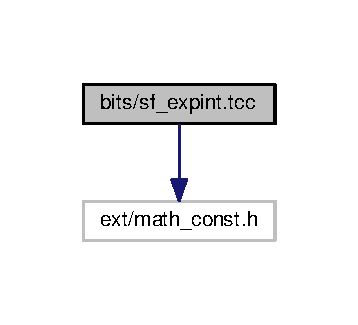
\includegraphics[width=294pt]{sf__expint_8tcc__incl}
\end{center}
\end{figure}
\doxysubsection*{Namespaces}
\begin{DoxyCompactItemize}
\item 
 \mbox{\hyperlink{namespaceemsr}{emsr}}
\item 
 \mbox{\hyperlink{namespaceemsr_1_1detail}{emsr\+::detail}}
\end{DoxyCompactItemize}
\doxysubsection*{Macros}
\begin{DoxyCompactItemize}
\item 
\#define \mbox{\hyperlink{sf__expint_8tcc_ab2687d13b3a8f9a0129346dd01a06b70}{SF\+\_\+\+EXPINT\+\_\+\+TCC}}~1
\end{DoxyCompactItemize}
\doxysubsection*{Functions}
\begin{DoxyCompactItemize}
\item 
{\footnotesize template$<$typename Tp $>$ }\\Tp \mbox{\hyperlink{namespaceemsr_1_1detail_a6c7ccfab06eace395ea765c510da2768}{emsr\+::detail\+::coshint}} (const Tp x)
\begin{DoxyCompactList}\small\item\em Return the hyperbolic cosine integral $ Chi(x) $. \end{DoxyCompactList}\item 
{\footnotesize template$<$typename Tp $>$ }\\Tp \mbox{\hyperlink{namespaceemsr_1_1detail_ab05351a08e3bd1ef244f97d8543ca9c0}{emsr\+::detail\+::expint}} (Tp x)
\begin{DoxyCompactList}\small\item\em Return the exponential integral $ Ei(x) $. \end{DoxyCompactList}\item 
{\footnotesize template$<$typename Tp $>$ }\\Tp \mbox{\hyperlink{namespaceemsr_1_1detail_a766c0e20c1b28670a42dbf224e03ce6a}{emsr\+::detail\+::expint}} (unsigned int n, Tp x)
\begin{DoxyCompactList}\small\item\em Return the exponential integral $ E_n(x) $. \end{DoxyCompactList}\item 
{\footnotesize template$<$typename Tp $>$ }\\Tp \mbox{\hyperlink{namespaceemsr_1_1detail_a73f0059aa33d1c8668b997c92462690b}{emsr\+::detail\+::expint\+\_\+\+E1}} (Tp x)
\begin{DoxyCompactList}\small\item\em Return the exponential integral $ E_1(x) $. \end{DoxyCompactList}\item 
{\footnotesize template$<$typename Tp $>$ }\\Tp \mbox{\hyperlink{namespaceemsr_1_1detail_addc426ee62b6017199c7f1f232c53f0e}{emsr\+::detail\+::expint\+\_\+\+E1\+\_\+asymp}} (Tp x)
\begin{DoxyCompactList}\small\item\em Return the exponential integral $ E_1(x) $ by asymptotic expansion. \end{DoxyCompactList}\item 
{\footnotesize template$<$typename Tp $>$ }\\Tp \mbox{\hyperlink{namespaceemsr_1_1detail_a60ccc644e299b81b9395d569294a6b58}{emsr\+::detail\+::expint\+\_\+\+E1\+\_\+series}} (Tp x)
\begin{DoxyCompactList}\small\item\em Return the exponential integral $ E_1(x) $ by series summation. This should be good for $ x < 1 $. \end{DoxyCompactList}\item 
{\footnotesize template$<$typename Tp $>$ }\\Tp \mbox{\hyperlink{namespaceemsr_1_1detail_ab0fd1bd71f8ab404ee8a02da2dfc5bc5}{emsr\+::detail\+::expint\+\_\+\+Ei}} (Tp x)
\begin{DoxyCompactList}\small\item\em Return the exponential integral $ Ei(x) $. \end{DoxyCompactList}\item 
{\footnotesize template$<$typename Tp $>$ }\\Tp \mbox{\hyperlink{namespaceemsr_1_1detail_aee98befc6c2a03d277770a9ff184e31c}{emsr\+::detail\+::expint\+\_\+\+Ei\+\_\+asymp}} (Tp x)
\begin{DoxyCompactList}\small\item\em Return the exponential integral $ Ei(x) $ by asymptotic expansion. \end{DoxyCompactList}\item 
{\footnotesize template$<$typename Tp $>$ }\\Tp \mbox{\hyperlink{namespaceemsr_1_1detail_a045f0bb6e64317b6dc9a666b664cad0a}{emsr\+::detail\+::expint\+\_\+\+Ei\+\_\+series}} (Tp x)
\begin{DoxyCompactList}\small\item\em Return the exponential integral $ Ei(x) $ by series summation. \end{DoxyCompactList}\item 
{\footnotesize template$<$typename Tp $>$ }\\Tp \mbox{\hyperlink{namespaceemsr_1_1detail_a0c26fe0ea5763127e613be2791b7ae86}{emsr\+::detail\+::expint\+\_\+\+En\+\_\+asymp}} (unsigned int n, Tp x)
\begin{DoxyCompactList}\small\item\em Return the exponential integral $ E_n(x) $ for large argument. \end{DoxyCompactList}\item 
{\footnotesize template$<$typename Tp $>$ }\\Tp \mbox{\hyperlink{namespaceemsr_1_1detail_abf7478e81614f20c9f0c72fc6ceb70a4}{emsr\+::detail\+::expint\+\_\+\+En\+\_\+cont\+\_\+frac}} (unsigned int n, Tp x)
\begin{DoxyCompactList}\small\item\em Return the exponential integral $ E_n(x) $ by continued fractions. \end{DoxyCompactList}\item 
{\footnotesize template$<$typename Tp $>$ }\\Tp \mbox{\hyperlink{namespaceemsr_1_1detail_a54fda585956818aed77e8724c3e875dd}{emsr\+::detail\+::expint\+\_\+\+En\+\_\+large\+\_\+n}} (unsigned int n, Tp x)
\begin{DoxyCompactList}\small\item\em Return the exponential integral $ E_n(x) $ for large order. \end{DoxyCompactList}\item 
{\footnotesize template$<$typename Tp $>$ }\\Tp \mbox{\hyperlink{namespaceemsr_1_1detail_a1601239a0f3c3df051f9eb73b7929a62}{emsr\+::detail\+::expint\+\_\+\+En\+\_\+recursion}} (unsigned int n, Tp x)
\begin{DoxyCompactList}\small\item\em Return the exponential integral $ E_n(x) $ by recursion. Use upward recursion for $ x < n $ and downward recursion (Miller\textquotesingle{}s algorithm) otherwise. \end{DoxyCompactList}\item 
{\footnotesize template$<$typename Tp $>$ }\\Tp \mbox{\hyperlink{namespaceemsr_1_1detail_a7e45acb12185a4b5728455cc4a70db3a}{emsr\+::detail\+::expint\+\_\+\+En\+\_\+series}} (unsigned int n, Tp x)
\begin{DoxyCompactList}\small\item\em Return the exponential integral $ E_n(x) $ by series summation. \end{DoxyCompactList}\item 
{\footnotesize template$<$typename Tp $>$ }\\Tp \mbox{\hyperlink{namespaceemsr_1_1detail_ae4d776e456675f7f9c75e715e0f2a3e6}{emsr\+::detail\+::logint}} (const Tp x)
\begin{DoxyCompactList}\small\item\em Return the logarithmic integral $ li(x) $. \end{DoxyCompactList}\item 
{\footnotesize template$<$typename Tp $>$ }\\Tp \mbox{\hyperlink{namespaceemsr_1_1detail_a4b93444883ecb02a412e20056085a3e6}{emsr\+::detail\+::sinhint}} (const Tp x)
\begin{DoxyCompactList}\small\item\em Return the hyperbolic sine integral $ Shi(x) $. \end{DoxyCompactList}\end{DoxyCompactItemize}


\doxysubsection{Macro Definition Documentation}
\mbox{\Hypertarget{sf__expint_8tcc_ab2687d13b3a8f9a0129346dd01a06b70}\label{sf__expint_8tcc_ab2687d13b3a8f9a0129346dd01a06b70}} 
\index{sf\_expint.tcc@{sf\_expint.tcc}!SF\_EXPINT\_TCC@{SF\_EXPINT\_TCC}}
\index{SF\_EXPINT\_TCC@{SF\_EXPINT\_TCC}!sf\_expint.tcc@{sf\_expint.tcc}}
\doxysubsubsection{\texorpdfstring{SF\_EXPINT\_TCC}{SF\_EXPINT\_TCC}}
{\footnotesize\ttfamily \#define SF\+\_\+\+EXPINT\+\_\+\+TCC~1}



Definition at line 46 of file sf\+\_\+expint.\+tcc.


\hypertarget{sf__fresnel_8tcc}{}\section{bits/sf\+\_\+fresnel.tcc File Reference}
\label{sf__fresnel_8tcc}\index{bits/sf\+\_\+fresnel.\+tcc@{bits/sf\+\_\+fresnel.\+tcc}}
{\ttfamily \#include $<$complex$>$}\newline
{\ttfamily \#include $<$ext/math\+\_\+const.\+h$>$}\newline
Include dependency graph for sf\+\_\+fresnel.\+tcc\+:
\nopagebreak
\begin{figure}[H]
\begin{center}
\leavevmode
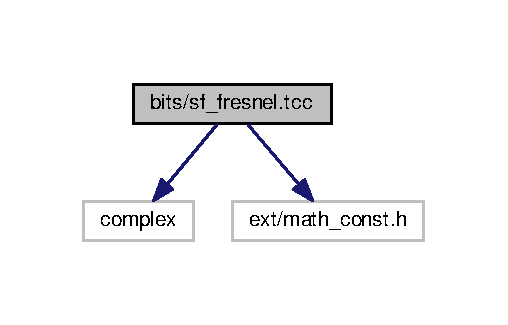
\includegraphics[width=244pt]{sf__fresnel_8tcc__incl}
\end{center}
\end{figure}
This graph shows which files directly or indirectly include this file\+:
\nopagebreak
\begin{figure}[H]
\begin{center}
\leavevmode
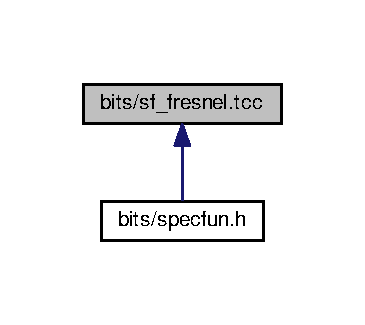
\includegraphics[width=175pt]{sf__fresnel_8tcc__dep__incl}
\end{center}
\end{figure}
\subsection*{Namespaces}
\begin{DoxyCompactItemize}
\item 
 \hyperlink{namespacestd}{std}
\item 
 \hyperlink{namespacestd_1_1____detail}{std\+::\+\_\+\+\_\+detail}
\begin{DoxyCompactList}\small\item\em Implementation-\/space details. \end{DoxyCompactList}\end{DoxyCompactItemize}
\subsection*{Macros}
\begin{DoxyCompactItemize}
\item 
\#define \hyperlink{sf__fresnel_8tcc_adbcd2dc06ad79716112c456abd18d171}{\+\_\+\+G\+L\+I\+B\+C\+X\+X\+\_\+\+B\+I\+T\+S\+\_\+\+S\+F\+\_\+\+F\+R\+E\+S\+N\+E\+L\+\_\+\+T\+CC}~1
\end{DoxyCompactItemize}
\subsection*{Functions}
\begin{DoxyCompactItemize}
\item 
{\footnotesize template$<$typename \+\_\+\+Tp $>$ }\\std\+::complex$<$ \+\_\+\+Tp $>$ \hyperlink{namespacestd_1_1____detail_a322045015cfbde5a45e7718d533de60d}{std\+::\+\_\+\+\_\+detail\+::\+\_\+\+\_\+fresnel} (const \+\_\+\+Tp \+\_\+\+\_\+x)
\begin{DoxyCompactList}\small\item\em Return the Fresnel cosine and sine integrals as a complex number \$f\mbox{[} C(x) + i\+S(x) \$f\mbox{]}. \end{DoxyCompactList}\item 
{\footnotesize template$<$typename \+\_\+\+Tp $>$ }\\void \hyperlink{namespacestd_1_1____detail_aeae8420e2fa1671f004066525adc99b6}{std\+::\+\_\+\+\_\+detail\+::\+\_\+\+\_\+fresnel\+\_\+cont\+\_\+frac} (const \+\_\+\+Tp \+\_\+\+\_\+ax, \+\_\+\+Tp \&\+\_\+\+Cf, \+\_\+\+Tp \&\+\_\+\+Sf)
\begin{DoxyCompactList}\small\item\em This function computes the Fresnel cosine and sine integrals by continued fractions for positive argument. \end{DoxyCompactList}\item 
{\footnotesize template$<$typename \+\_\+\+Tp $>$ }\\void \hyperlink{namespacestd_1_1____detail_aae7775bc46d621e54fb9d994c2f35e2a}{std\+::\+\_\+\+\_\+detail\+::\+\_\+\+\_\+fresnel\+\_\+series} (const \+\_\+\+Tp \+\_\+\+\_\+ax, \+\_\+\+Tp \&\+\_\+\+Cf, \+\_\+\+Tp \&\+\_\+\+Sf)
\begin{DoxyCompactList}\small\item\em This function returns the Fresnel cosine and sine integrals as a pair by series expansion for positive argument. \end{DoxyCompactList}\end{DoxyCompactItemize}


\subsection{Detailed Description}
This is an internal header file, included by other library headers. Do not attempt to use it directly. Instead, include $<$cmath$>$. 

\subsection{Macro Definition Documentation}
\mbox{\Hypertarget{sf__fresnel_8tcc_adbcd2dc06ad79716112c456abd18d171}\label{sf__fresnel_8tcc_adbcd2dc06ad79716112c456abd18d171}} 
\index{sf\+\_\+fresnel.\+tcc@{sf\+\_\+fresnel.\+tcc}!\+\_\+\+G\+L\+I\+B\+C\+X\+X\+\_\+\+B\+I\+T\+S\+\_\+\+S\+F\+\_\+\+F\+R\+E\+S\+N\+E\+L\+\_\+\+T\+CC@{\+\_\+\+G\+L\+I\+B\+C\+X\+X\+\_\+\+B\+I\+T\+S\+\_\+\+S\+F\+\_\+\+F\+R\+E\+S\+N\+E\+L\+\_\+\+T\+CC}}
\index{\+\_\+\+G\+L\+I\+B\+C\+X\+X\+\_\+\+B\+I\+T\+S\+\_\+\+S\+F\+\_\+\+F\+R\+E\+S\+N\+E\+L\+\_\+\+T\+CC@{\+\_\+\+G\+L\+I\+B\+C\+X\+X\+\_\+\+B\+I\+T\+S\+\_\+\+S\+F\+\_\+\+F\+R\+E\+S\+N\+E\+L\+\_\+\+T\+CC}!sf\+\_\+fresnel.\+tcc@{sf\+\_\+fresnel.\+tcc}}
\subsubsection{\texorpdfstring{\+\_\+\+G\+L\+I\+B\+C\+X\+X\+\_\+\+B\+I\+T\+S\+\_\+\+S\+F\+\_\+\+F\+R\+E\+S\+N\+E\+L\+\_\+\+T\+CC}{\_GLIBCXX\_BITS\_SF\_FRESNEL\_TCC}}
{\footnotesize\ttfamily \#define \+\_\+\+G\+L\+I\+B\+C\+X\+X\+\_\+\+B\+I\+T\+S\+\_\+\+S\+F\+\_\+\+F\+R\+E\+S\+N\+E\+L\+\_\+\+T\+CC~1}



Definition at line 31 of file sf\+\_\+fresnel.\+tcc.


\hypertarget{sf__gamma_8tcc}{}\section{bits/sf\+\_\+gamma.tcc File Reference}
\label{sf__gamma_8tcc}\index{bits/sf\+\_\+gamma.\+tcc@{bits/sf\+\_\+gamma.\+tcc}}
{\ttfamily \#include $<$array$>$}\\*
{\ttfamily \#include $<$ext/math\+\_\+const.\+h$>$}\\*
Include dependency graph for sf\+\_\+gamma.\+tcc\+:
\nopagebreak
\begin{figure}[H]
\begin{center}
\leavevmode
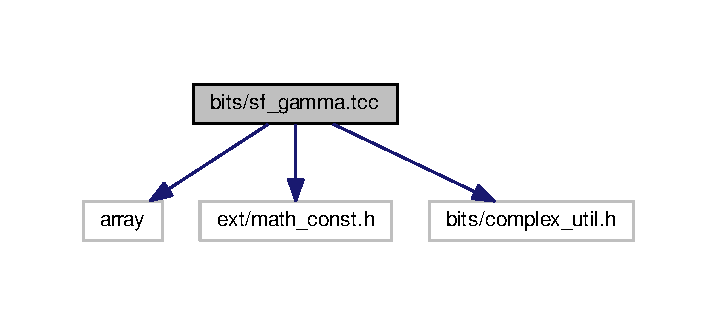
\includegraphics[width=228pt]{sf__gamma_8tcc__incl}
\end{center}
\end{figure}
This graph shows which files directly or indirectly include this file\+:
\nopagebreak
\begin{figure}[H]
\begin{center}
\leavevmode
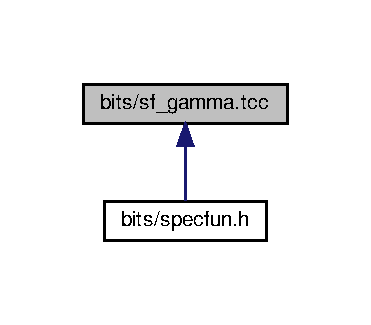
\includegraphics[width=178pt]{sf__gamma_8tcc__dep__incl}
\end{center}
\end{figure}
\subsection*{Classes}
\begin{DoxyCompactItemize}
\item 
struct \hyperlink{structstd_1_1____detail_1_1__Factorial__table}{std\+::\+\_\+\+\_\+detail\+::\+\_\+\+Factorial\+\_\+table$<$ \+\_\+\+Tp $>$}
\item 
struct \hyperlink{structstd_1_1____detail_1_1__GammaLanczos}{std\+::\+\_\+\+\_\+detail\+::\+\_\+\+Gamma\+Lanczos$<$ \+\_\+\+Tp $>$}
\item 
struct \hyperlink{structstd_1_1____detail_1_1__GammaLanczos_3_01double_01_4}{std\+::\+\_\+\+\_\+detail\+::\+\_\+\+Gamma\+Lanczos$<$ double $>$}
\item 
struct \hyperlink{structstd_1_1____detail_1_1__GammaLanczos_3_01float_01_4}{std\+::\+\_\+\+\_\+detail\+::\+\_\+\+Gamma\+Lanczos$<$ float $>$}
\item 
struct \hyperlink{structstd_1_1____detail_1_1__GammaLanczos_3_01long_01double_01_4}{std\+::\+\_\+\+\_\+detail\+::\+\_\+\+Gamma\+Lanczos$<$ long double $>$}
\item 
struct \hyperlink{structstd_1_1____detail_1_1__GammaSpouge}{std\+::\+\_\+\+\_\+detail\+::\+\_\+\+Gamma\+Spouge$<$ \+\_\+\+Tp $>$}
\item 
struct \hyperlink{structstd_1_1____detail_1_1__GammaSpouge_3_01double_01_4}{std\+::\+\_\+\+\_\+detail\+::\+\_\+\+Gamma\+Spouge$<$ double $>$}
\item 
struct \hyperlink{structstd_1_1____detail_1_1__GammaSpouge_3_01float_01_4}{std\+::\+\_\+\+\_\+detail\+::\+\_\+\+Gamma\+Spouge$<$ float $>$}
\item 
struct \hyperlink{structstd_1_1____detail_1_1__GammaSpouge_3_01long_01double_01_4}{std\+::\+\_\+\+\_\+detail\+::\+\_\+\+Gamma\+Spouge$<$ long double $>$}
\end{DoxyCompactItemize}
\subsection*{Namespaces}
\begin{DoxyCompactItemize}
\item 
 \hyperlink{namespacestd}{std}
\item 
 \hyperlink{namespacestd_1_1____detail}{std\+::\+\_\+\+\_\+detail}
\end{DoxyCompactItemize}
\subsection*{Macros}
\begin{DoxyCompactItemize}
\item 
\#define \hyperlink{sf__gamma_8tcc_accc383e52e4dc6eebfd313a52961b49b}{\+\_\+\+G\+L\+I\+B\+C\+X\+X\+\_\+\+B\+I\+T\+S\+\_\+\+S\+F\+\_\+\+G\+A\+M\+M\+A\+\_\+\+T\+CC}~1
\end{DoxyCompactItemize}
\subsection*{Functions}
\begin{DoxyCompactItemize}
\item 
{\footnotesize template$<$typename \+\_\+\+Tp $>$ }\\\+\_\+\+G\+L\+I\+B\+C\+X\+X14\+\_\+\+C\+O\+N\+S\+T\+E\+X\+PR \+\_\+\+Tp \hyperlink{namespacestd_1_1____detail_a5dc6cb42a6bcd3258371b6cc93ee12f0}{std\+::\+\_\+\+\_\+detail\+::\+\_\+\+\_\+bernoulli} (int \+\_\+\+\_\+n)
\begin{DoxyCompactList}\small\item\em This returns Bernoulli number $ B_n $. \end{DoxyCompactList}\item 
{\footnotesize template$<$typename \+\_\+\+Tp $>$ }\\\+\_\+\+G\+L\+I\+B\+C\+X\+X14\+\_\+\+C\+O\+N\+S\+T\+E\+X\+PR \+\_\+\+Tp \hyperlink{namespacestd_1_1____detail_a72c7ddb85ace9619af583ca2acdb0a9b}{std\+::\+\_\+\+\_\+detail\+::\+\_\+\+\_\+bernoulli\+\_\+2n} (int \+\_\+\+\_\+n)
\begin{DoxyCompactList}\small\item\em This returns Bernoulli number $ B_2n $ at even integer arguments $ 2n $. \end{DoxyCompactList}\item 
{\footnotesize template$<$typename \+\_\+\+Tp $>$ }\\\+\_\+\+G\+L\+I\+B\+C\+X\+X14\+\_\+\+C\+O\+N\+S\+T\+E\+X\+PR \+\_\+\+Tp \hyperlink{namespacestd_1_1____detail_ad3d3e44d340742b0362a8ad95080d315}{std\+::\+\_\+\+\_\+detail\+::\+\_\+\+\_\+bernoulli\+\_\+series} (unsigned int \+\_\+\+\_\+n)
\begin{DoxyCompactList}\small\item\em This returns Bernoulli numbers from a table or by summation for larger values. \end{DoxyCompactList}\item 
{\footnotesize template$<$typename \+\_\+\+Tp $>$ }\\\+\_\+\+Tp \hyperlink{namespacestd_1_1____detail_ab0888bd3901e6501b1f451d6adcf967a}{std\+::\+\_\+\+\_\+detail\+::\+\_\+\+\_\+bincoef} (unsigned int \+\_\+\+\_\+n, unsigned int \+\_\+\+\_\+k)
\begin{DoxyCompactList}\small\item\em Return the binomial coefficient. The binomial coefficient is given by\+: \[ \binom{n}{k} = \frac{n!}{(n-k)! k!} \] The binomial coefficients are generated by\+: \[ \left(1 + t\right)^n = \sum_{k=0}^n \binom{n}{k} t^k \]. \end{DoxyCompactList}\item 
{\footnotesize template$<$typename \+\_\+\+Tp $>$ }\\\+\_\+\+Tp \hyperlink{namespacestd_1_1____detail_a537c9234f68801f2cdb60020cb98fbbd}{std\+::\+\_\+\+\_\+detail\+::\+\_\+\+\_\+bincoef} (\+\_\+\+Tp \+\_\+\+\_\+nu, unsigned int \+\_\+\+\_\+k)
\begin{DoxyCompactList}\small\item\em Return the binomial coefficient for non-\/integral degree. The binomial coefficient is given by\+: \[ \binom{\nu}{k} = \frac{\Gamma(\nu+1)}{\Gamma(\nu-k+1) \Gamma(k+1)} \] The binomial coefficients are generated by\+: \[ \left(1 + t\right)^\nu = \sum_{k=0}^\infty \binom{\nu}{k} t^k \]. \end{DoxyCompactList}\item 
{\footnotesize template$<$typename \+\_\+\+Tp $>$ }\\\+\_\+\+G\+L\+I\+B\+C\+X\+X14\+\_\+\+C\+O\+N\+S\+T\+E\+X\+PR \+\_\+\+Tp \hyperlink{namespacestd_1_1____detail_a06b0d9786afff0919c96f61d5f760c5f}{std\+::\+\_\+\+\_\+detail\+::\+\_\+\+\_\+double\+\_\+factorial} (int \+\_\+\+\_\+n)
\begin{DoxyCompactList}\small\item\em Return the double factorial of the integer n. \end{DoxyCompactList}\item 
{\footnotesize template$<$typename \+\_\+\+Tp $>$ }\\\+\_\+\+G\+L\+I\+B\+C\+X\+X14\+\_\+\+C\+O\+N\+S\+T\+E\+X\+PR \+\_\+\+Tp \hyperlink{namespacestd_1_1____detail_a8de5d6069cbef126684be0800f47f8b2}{std\+::\+\_\+\+\_\+detail\+::\+\_\+\+\_\+factorial} (unsigned int \+\_\+\+\_\+n)
\begin{DoxyCompactList}\small\item\em Return the factorial of the integer n. \end{DoxyCompactList}\item 
{\footnotesize template$<$typename \+\_\+\+Tp $>$ }\\\+\_\+\+Tp \hyperlink{namespacestd_1_1____detail_aa0e76080654c918631595a7da642913f}{std\+::\+\_\+\+\_\+detail\+::\+\_\+\+\_\+gamma} (\+\_\+\+Tp \+\_\+\+\_\+x)
\begin{DoxyCompactList}\small\item\em Return the gamma function $ \Gamma(x) $. The gamma function is defined by\+: \[ \Gamma(a) = \int_0^\infty e^{-t}t^{a-1}dt (a > 0) \]. \end{DoxyCompactList}\item 
{\footnotesize template$<$typename \+\_\+\+Tp $>$ }\\std\+::pair$<$ \+\_\+\+Tp, \+\_\+\+Tp $>$ \hyperlink{namespacestd_1_1____detail_afd6319747af991947a02388acee40c26}{std\+::\+\_\+\+\_\+detail\+::\+\_\+\+\_\+gamma\+\_\+cont\+\_\+frac} (\+\_\+\+Tp \+\_\+\+\_\+a, \+\_\+\+Tp \+\_\+\+\_\+x)
\begin{DoxyCompactList}\small\item\em Return the incomplete gamma function by continued fraction. \end{DoxyCompactList}\item 
{\footnotesize template$<$typename \+\_\+\+Tp $>$ }\\std\+::pair$<$ \+\_\+\+Tp, \+\_\+\+Tp $>$ \hyperlink{namespacestd_1_1____detail_aa480c595e1c5b894d76398cf0e8eb02b}{std\+::\+\_\+\+\_\+detail\+::\+\_\+\+\_\+gamma\+\_\+series} (\+\_\+\+Tp \+\_\+\+\_\+a, \+\_\+\+Tp \+\_\+\+\_\+x)
\begin{DoxyCompactList}\small\item\em Return the incomplete gamma function by series summation. \end{DoxyCompactList}\item 
{\footnotesize template$<$typename \+\_\+\+Tp $>$ }\\\+\_\+\+Tp \hyperlink{namespacestd_1_1____detail_aeab2857a72e09b180a765bf435f72c2e}{std\+::\+\_\+\+\_\+detail\+::\+\_\+\+\_\+harmonic\+\_\+number} (unsigned int \+\_\+\+\_\+n)
\item 
{\footnotesize template$<$typename \+\_\+\+Tp $>$ }\\\+\_\+\+Tp \hyperlink{namespacestd_1_1____detail_a152324942f37ae3c6fc65aec1f17049e}{std\+::\+\_\+\+\_\+detail\+::\+\_\+\+\_\+log\+\_\+bincoef} (unsigned int \+\_\+\+\_\+n, unsigned int \+\_\+\+\_\+k)
\begin{DoxyCompactList}\small\item\em Return the logarithm of the binomial coefficient. The binomial coefficient is given by\+: \[ \binom{n}{k} = \frac{n!}{(n-k)! k!} \] The binomial coefficients are generated by\+: \[ \left(1 + t\right)^n = \sum_{k=0}^n \binom{n}{k} t^k \]. \end{DoxyCompactList}\item 
{\footnotesize template$<$typename \+\_\+\+Tp $>$ }\\\+\_\+\+Tp \hyperlink{namespacestd_1_1____detail_abd174c4887c0f3bbb5125e2a65856386}{std\+::\+\_\+\+\_\+detail\+::\+\_\+\+\_\+log\+\_\+bincoef} (\+\_\+\+Tp \+\_\+\+\_\+nu, unsigned int \+\_\+\+\_\+k)
\begin{DoxyCompactList}\small\item\em Return the logarithm of the binomial coefficient for non-\/integral degree. The binomial coefficient is given by\+: \[ \binom{\nu}{k} = \frac{\Gamma(\nu+1)}{\Gamma(\nu-k+1) \Gamma(k+1)} \] The binomial coefficients are generated by\+: \[ \left(1 + t\right)^\nu = \sum_{k=0}^\infty \binom{\nu}{k} t^k \]. \end{DoxyCompactList}\item 
{\footnotesize template$<$typename \+\_\+\+Tp $>$ }\\\+\_\+\+Tp \hyperlink{namespacestd_1_1____detail_a6cea85f06264c3c9b05a76012205a0ca}{std\+::\+\_\+\+\_\+detail\+::\+\_\+\+\_\+log\+\_\+bincoef\+\_\+sign} (\+\_\+\+Tp \+\_\+\+\_\+nu, unsigned int \+\_\+\+\_\+k)
\begin{DoxyCompactList}\small\item\em Return the sign of $ \Gamma(x) $. At nonpositive integers zero is returned. \end{DoxyCompactList}\item 
{\footnotesize template$<$typename \+\_\+\+Tp $>$ }\\std\+::complex$<$ \+\_\+\+Tp $>$ \hyperlink{namespacestd_1_1____detail_acaa1cf71cfd1d1ec4e897a9b9d10e8a1}{std\+::\+\_\+\+\_\+detail\+::\+\_\+\+\_\+log\+\_\+bincoef\+\_\+sign} (std\+::complex$<$ \+\_\+\+Tp $>$ \+\_\+\+\_\+nu, unsigned int \+\_\+\+\_\+k)
\item 
{\footnotesize template$<$typename \+\_\+\+Tp $>$ }\\\+\_\+\+G\+L\+I\+B\+C\+X\+X14\+\_\+\+C\+O\+N\+S\+T\+E\+X\+PR \+\_\+\+Tp \hyperlink{namespacestd_1_1____detail_a0de46e790512550b535bdda97e11e1b5}{std\+::\+\_\+\+\_\+detail\+::\+\_\+\+\_\+log\+\_\+double\+\_\+factorial} (\+\_\+\+Tp \+\_\+\+\_\+x)
\item 
{\footnotesize template$<$typename \+\_\+\+Tp $>$ }\\\+\_\+\+G\+L\+I\+B\+C\+X\+X14\+\_\+\+C\+O\+N\+S\+T\+E\+X\+PR \+\_\+\+Tp \hyperlink{namespacestd_1_1____detail_aa832ed1d29fd41c40cf892cc1feef7e9}{std\+::\+\_\+\+\_\+detail\+::\+\_\+\+\_\+log\+\_\+double\+\_\+factorial} (int \+\_\+\+\_\+n)
\begin{DoxyCompactList}\small\item\em Return the logarithm of the double factorial of the integer n. \end{DoxyCompactList}\item 
{\footnotesize template$<$typename \+\_\+\+Tp $>$ }\\\+\_\+\+G\+L\+I\+B\+C\+X\+X14\+\_\+\+C\+O\+N\+S\+T\+E\+X\+PR \+\_\+\+Tp \hyperlink{namespacestd_1_1____detail_a2809419dbbe9fc60066dacfdc13761d4}{std\+::\+\_\+\+\_\+detail\+::\+\_\+\+\_\+log\+\_\+factorial} (unsigned int \+\_\+\+\_\+n)
\begin{DoxyCompactList}\small\item\em Return the logarithm of the factorial of the integer n. \end{DoxyCompactList}\item 
{\footnotesize template$<$typename \+\_\+\+Tp $>$ }\\\+\_\+\+Tp \hyperlink{namespacestd_1_1____detail_aa8be6df2c5d12d0d1cb1f02a6b3592ef}{std\+::\+\_\+\+\_\+detail\+::\+\_\+\+\_\+log\+\_\+gamma} (\+\_\+\+Tp \+\_\+\+\_\+x)
\begin{DoxyCompactList}\small\item\em Return $ log(|\Gamma(x)|) $. This will return values even for $ x < 0 $. To recover the sign of $ \Gamma(x) $ for any argument use {\itshape \+\_\+\+\_\+log\+\_\+gamma\+\_\+sign}. \end{DoxyCompactList}\item 
{\footnotesize template$<$typename \+\_\+\+Tp $>$ }\\std\+::complex$<$ \+\_\+\+Tp $>$ \hyperlink{namespacestd_1_1____detail_a48b62f07d0a6ec04dd9132a1cd7850c9}{std\+::\+\_\+\+\_\+detail\+::\+\_\+\+\_\+log\+\_\+gamma} (std\+::complex$<$ \+\_\+\+Tp $>$ \+\_\+\+\_\+x)
\begin{DoxyCompactList}\small\item\em Return $ log(\Gamma(x)) $ for complex argument. \end{DoxyCompactList}\item 
{\footnotesize template$<$typename \+\_\+\+Tp $>$ }\\\+\_\+\+G\+L\+I\+B\+C\+X\+X14\+\_\+\+C\+O\+N\+S\+T\+E\+X\+PR \+\_\+\+Tp \hyperlink{namespacestd_1_1____detail_a7c30a619e78752c14417f05eaab283d3}{std\+::\+\_\+\+\_\+detail\+::\+\_\+\+\_\+log\+\_\+gamma1p\+\_\+lanczos} (\+\_\+\+Tp \+\_\+\+\_\+z)
\begin{DoxyCompactList}\small\item\em Return $log(\Gamma(x))$ by the Lanczos method. This method dominates all others on the positive axis I think. \end{DoxyCompactList}\item 
{\footnotesize template$<$typename \+\_\+\+Tp $>$ }\\\+\_\+\+G\+L\+I\+B\+C\+X\+X14\+\_\+\+C\+O\+N\+S\+T\+E\+X\+PR \+\_\+\+Tp \hyperlink{namespacestd_1_1____detail_aca3fe0938c60534a835aeddc82555a75}{std\+::\+\_\+\+\_\+detail\+::\+\_\+\+\_\+log\+\_\+gamma1p\+\_\+spouge} (\+\_\+\+Tp \+\_\+\+\_\+z)
\begin{DoxyCompactList}\small\item\em Return $\Gamma(z)$ by the Spouge algorithm\+: \[ \Gamma(z+1) = (z+a)^{z+1/2}e^{-z-a}\left[ \sqrt{2\pi} + \sum_{k=1}^{\lceil a \rceil + 1}\frac{c_k(a)}{z+k}\right] \] where \[ c_k(a) = \frac{(-1)^{k-1}}{(k-1)!}(a-k)^{k-1/2}e^{a-k} \] and the error is bounded by \[ \epsilon(a) < a^{-1/2}(2\pi)^{-a-1/2} \]. \end{DoxyCompactList}\item 
{\footnotesize template$<$typename \+\_\+\+Tp $>$ }\\\+\_\+\+G\+L\+I\+B\+C\+X\+X14\+\_\+\+C\+O\+N\+S\+T\+E\+X\+PR \+\_\+\+Tp \hyperlink{namespacestd_1_1____detail_ac13e31ebcd3c99d6a7cad9010e039315}{std\+::\+\_\+\+\_\+detail\+::\+\_\+\+\_\+log\+\_\+gamma\+\_\+bernoulli} (\+\_\+\+Tp \+\_\+\+\_\+x)
\begin{DoxyCompactList}\small\item\em Return $log(\Gamma(x))$ by asymptotic expansion with Bernoulli number coefficients. This is like Sterling\textquotesingle{}s approximation. \end{DoxyCompactList}\item 
{\footnotesize template$<$typename \+\_\+\+Tp $>$ }\\\+\_\+\+Tp \hyperlink{namespacestd_1_1____detail_ac091f187fbe5efdbc912ec9ca38ba25f}{std\+::\+\_\+\+\_\+detail\+::\+\_\+\+\_\+log\+\_\+gamma\+\_\+sign} (\+\_\+\+Tp \+\_\+\+\_\+x)
\begin{DoxyCompactList}\small\item\em Return the sign of $ \Gamma(x) $. At nonpositive integers zero is returned indicating $ \Gamma(x) $ is undefined. \end{DoxyCompactList}\item 
{\footnotesize template$<$typename \+\_\+\+Tp $>$ }\\std\+::complex$<$ \+\_\+\+Tp $>$ \hyperlink{namespacestd_1_1____detail_a775873eb710ac3f2d1dd774aba216795}{std\+::\+\_\+\+\_\+detail\+::\+\_\+\+\_\+log\+\_\+gamma\+\_\+sign} (std\+::complex$<$ \+\_\+\+Tp $>$ \+\_\+\+\_\+x)
\item 
{\footnotesize template$<$typename \+\_\+\+Tp $>$ }\\\+\_\+\+Tp \hyperlink{namespacestd_1_1____detail_afc646f25bed26aee2265d225ed29bce6}{std\+::\+\_\+\+\_\+detail\+::\+\_\+\+\_\+log\+\_\+pochhammer} (\+\_\+\+Tp \+\_\+\+\_\+a, \+\_\+\+Tp \+\_\+\+\_\+n)
\begin{DoxyCompactList}\small\item\em Return the logarithm of the (upper) Pochhammer symbol or the rising factorial function. The Pochammer symbol is defined for integer order by \[ (a)_n = \prod_{k=0}^{n-1} (a + k), (a)_0 = 1 = \Gamma(a + n) / \Gamma(n) \] Thus this function returns \[ ln[(a)_n] = \Gamma(a + n) - \Gamma(n), ln[(a)_0] = 0 \] Many notations exist\+: \[ a^{\overline{n}} \], \[ \left[ \begin{array}{c} a \\ n \end{array} \right] \], and others. \end{DoxyCompactList}\item 
{\footnotesize template$<$typename \+\_\+\+Tp $>$ }\\\+\_\+\+Tp \hyperlink{namespacestd_1_1____detail_ab3932d3e5a5be73ea2022d80b065df4a}{std\+::\+\_\+\+\_\+detail\+::\+\_\+\+\_\+log\+\_\+pochhammer\+\_\+lower} (\+\_\+\+Tp \+\_\+\+\_\+a, \+\_\+\+Tp \+\_\+\+\_\+n)
\begin{DoxyCompactList}\small\item\em Return the logarithm of the lower Pochhammer symbol or the falling factorial function. The lower Pochammer symbol is defined by \[ (a)_n = \prod_{k=0}^{n-1} (a - k), (a)_0 = 1 = \Gamma(a + 1) / \Gamma(a - n + 1) \] In particular, \$f\mbox{[} (n)\+\_\+n = n! \$f\mbox{]}. Thus this function returns \[ ln[(a)_n] = \Gamma(a + 1) - \Gamma(a - n + 1), ln[(a)_0] = 0 \] Many notations exist\+: \[ a^{\underline{n}} \], \[ \{ \begin{array}{c} a \\ n \end{array} \} \], and others. \end{DoxyCompactList}\item 
{\footnotesize template$<$typename \+\_\+\+Tp $>$ }\\\+\_\+\+Tp \hyperlink{namespacestd_1_1____detail_a009273f90a2496eb24abf92cd957b851}{std\+::\+\_\+\+\_\+detail\+::\+\_\+\+\_\+pgamma} (\+\_\+\+Tp \+\_\+\+\_\+a, \+\_\+\+Tp \+\_\+\+\_\+x)
\begin{DoxyCompactList}\small\item\em Return the regularized lower incomplete gamma function. The regularized lower incomplete gamma function is defined by \[ P(a,x) = \frac{\gamma(a,x)}{\Gamma(a)} \] where $ \Gamma(a) $ is the gamma function and \[ \gamma(a,x) = \int_0^x e^{-t}t^{a-1}dt (a > 0) \] is the lower incomplete gamma function. \end{DoxyCompactList}\item 
{\footnotesize template$<$typename \+\_\+\+Tp $>$ }\\\+\_\+\+Tp \hyperlink{namespacestd_1_1____detail_ae1fb9f383f9b657f76d0c183ecd6ae29}{std\+::\+\_\+\+\_\+detail\+::\+\_\+\+\_\+pochhammer} (\+\_\+\+Tp \+\_\+\+\_\+a, \+\_\+\+Tp \+\_\+\+\_\+n)
\begin{DoxyCompactList}\small\item\em Return the (upper) Pochhammer function or the rising factorial function. The Pochammer symbol is defined by \[ (a)_n = \prod_{k=0}^{n-1} (a + k), (a)_0 = 1 = \Gamma(a + n) / \Gamma(n) \] Many notations exist\+: \[ a^{\overline{n}} \], \[ \left[ \begin{array}{c} a \\ n \end{array} \right] \], and others. \end{DoxyCompactList}\item 
{\footnotesize template$<$typename \+\_\+\+Tp $>$ }\\\+\_\+\+Tp \hyperlink{namespacestd_1_1____detail_acd08cb0905b67d8a6a1c29fa5d46ec88}{std\+::\+\_\+\+\_\+detail\+::\+\_\+\+\_\+pochhammer\+\_\+lower} (\+\_\+\+Tp \+\_\+\+\_\+a, \+\_\+\+Tp \+\_\+\+\_\+n)
\begin{DoxyCompactList}\small\item\em Return the logarithm of the lower Pochhammer symbol or the falling factorial function. The lower Pochammer symbol is defined by \[ (a)_n = \prod_{k=0}^{n-1} (a - k), (a)_0 = 1 = \Gamma(a + 1) / \Gamma(a - n + 1) \] In particular, \$f\mbox{[} (n)\+\_\+n = n! \$f\mbox{]}. \end{DoxyCompactList}\item 
{\footnotesize template$<$typename \+\_\+\+Tp $>$ }\\\+\_\+\+Tp \hyperlink{namespacestd_1_1____detail_a664d83a211283d0975ba40f3874c2d70}{std\+::\+\_\+\+\_\+detail\+::\+\_\+\+\_\+psi} (unsigned int \+\_\+\+\_\+n)
\begin{DoxyCompactList}\small\item\em Return the digamma function of integral argument. The digamma or $ \psi(x) $ function is defined as the logarithmic derivative of the gamma function\+: \[ \psi(x) = \frac{\Gamma'(x)}{\Gamma(x)} \] The digamma series for integral argument is given by\+: \[ \psi(n) = -\gamma_E + \sum_{k=1}^{\infty} \frac{1}{k} \] The latter sum is called the harmonic number, $ H_n $. \end{DoxyCompactList}\item 
{\footnotesize template$<$typename \+\_\+\+Tp $>$ }\\\+\_\+\+Tp \hyperlink{namespacestd_1_1____detail_ad7246a3ca90be800e6cc79c8e2360abd}{std\+::\+\_\+\+\_\+detail\+::\+\_\+\+\_\+psi} (\+\_\+\+Tp \+\_\+\+\_\+x)
\begin{DoxyCompactList}\small\item\em Return the digamma function. The digamma or $ \psi(x) $ function is defined by \[ \psi(x) = \frac{\Gamma'(x)}{\Gamma(x)} \] For negative argument the reflection formula is used\+: \[ \psi(x) = \psi(1-x) - \pi \cot(\pi x) \]. \end{DoxyCompactList}\item 
{\footnotesize template$<$typename \+\_\+\+Tp $>$ }\\\+\_\+\+Tp \hyperlink{namespacestd_1_1____detail_a96d6b8301ca54615364a53665b347f6c}{std\+::\+\_\+\+\_\+detail\+::\+\_\+\+\_\+psi} (unsigned int \+\_\+\+\_\+n, \+\_\+\+Tp \+\_\+\+\_\+x)
\begin{DoxyCompactList}\small\item\em Return the polygamma function $ \psi^{(n)}(x) $. \end{DoxyCompactList}\item 
{\footnotesize template$<$typename \+\_\+\+Tp $>$ }\\\+\_\+\+Tp \hyperlink{namespacestd_1_1____detail_a2557b5d815b6667bc9228c1e8a2a16ae}{std\+::\+\_\+\+\_\+detail\+::\+\_\+\+\_\+psi\+\_\+asymp} (\+\_\+\+Tp \+\_\+\+\_\+x)
\begin{DoxyCompactList}\small\item\em Return the digamma function for large argument. The digamma or $ \psi(x) $ function is defined by \[ \psi(x) = \frac{\Gamma'(x)}{\Gamma(x)} \]. \end{DoxyCompactList}\item 
{\footnotesize template$<$typename \+\_\+\+Tp $>$ }\\\+\_\+\+Tp \hyperlink{namespacestd_1_1____detail_a378e78e1c3c08b8f146acf32a26e831a}{std\+::\+\_\+\+\_\+detail\+::\+\_\+\+\_\+psi\+\_\+series} (\+\_\+\+Tp \+\_\+\+\_\+x)
\begin{DoxyCompactList}\small\item\em Return the digamma function by series expansion. The digamma or $ \psi(x) $ function is defined by \[ \psi(x) = \frac{\Gamma'(x)}{\Gamma(x)} \]. \end{DoxyCompactList}\item 
{\footnotesize template$<$typename \+\_\+\+Tp $>$ }\\\+\_\+\+Tp \hyperlink{namespacestd_1_1____detail_acaac94504608c15edb7d96884ac1dc23}{std\+::\+\_\+\+\_\+detail\+::\+\_\+\+\_\+qgamma} (\+\_\+\+Tp \+\_\+\+\_\+a, \+\_\+\+Tp \+\_\+\+\_\+x)
\begin{DoxyCompactList}\small\item\em Return the regularized upper incomplete gamma function. The regularized upper incomplete gamma function is defined by \[ Q(a,x) = \frac{\Gamma(a,x)}{\Gamma(a)} \] where $ \Gamma(a) $ is the gamma function and \[ \Gamma(a,x) = \int_x^\infty e^{-t}t^{a-1}dt (a > 0) \] is the upper incomplete gamma function. \end{DoxyCompactList}\item 
{\footnotesize template$<$typename \+\_\+\+Tp $>$ }\\\+\_\+\+Tp \hyperlink{namespacestd_1_1____detail_ad2f6546e22348b07d992d522153d7d6b}{std\+::\+\_\+\+\_\+detail\+::\+\_\+\+\_\+tgamma} (\+\_\+\+Tp \+\_\+\+\_\+a, \+\_\+\+Tp \+\_\+\+\_\+x)
\begin{DoxyCompactList}\small\item\em Return the upper incomplete gamma function. The lower incomplete gamma function is defined by \[ \Gamma(a,x) = \int_x^\infty e^{-t}t^{a-1}dt (a > 0) \]. \end{DoxyCompactList}\item 
{\footnotesize template$<$typename \+\_\+\+Tp $>$ }\\\+\_\+\+Tp \hyperlink{namespacestd_1_1____detail_ad85ad5ffdb1bab9b1e3b6fd7a114fb0d}{std\+::\+\_\+\+\_\+detail\+::\+\_\+\+\_\+tgamma\+\_\+lower} (\+\_\+\+Tp \+\_\+\+\_\+a, \+\_\+\+Tp \+\_\+\+\_\+x)
\begin{DoxyCompactList}\small\item\em Return the lower incomplete gamma function. The lower incomplete gamma function is defined by \[ \gamma(a,x) = \int_0^x e^{-t}t^{a-1}dt (a > 0) \]. \end{DoxyCompactList}\end{DoxyCompactItemize}
\subsection*{Variables}
\begin{DoxyCompactItemize}
\item 
constexpr \+\_\+\+Factorial\+\_\+table$<$ long double $>$ \hyperlink{namespacestd_1_1____detail_a6d1131fefdb30b2746c76ff801bdc833}{std\+::\+\_\+\+\_\+detail\+::\+\_\+\+S\+\_\+double\+\_\+factorial\+\_\+table} \mbox{[}301\mbox{]}
\item 
constexpr \+\_\+\+Factorial\+\_\+table$<$ long double $>$ \hyperlink{namespacestd_1_1____detail_a008b54abe31c1027aefdfd7a76a40e99}{std\+::\+\_\+\+\_\+detail\+::\+\_\+\+S\+\_\+factorial\+\_\+table} \mbox{[}171\mbox{]}
\item 
constexpr unsigned long long \hyperlink{namespacestd_1_1____detail_ad2bdb66d93fa4433097b287c7899cd1e}{std\+::\+\_\+\+\_\+detail\+::\+\_\+\+S\+\_\+harmonic\+\_\+denom} \mbox{[}\+\_\+\+S\+\_\+num\+\_\+harmonic\+\_\+numer\mbox{]}
\item 
constexpr unsigned long long \hyperlink{namespacestd_1_1____detail_a3976bb1731d7ecfaba4601d1083d7cf6}{std\+::\+\_\+\+\_\+detail\+::\+\_\+\+S\+\_\+harmonic\+\_\+numer} \mbox{[}\+\_\+\+S\+\_\+num\+\_\+harmonic\+\_\+numer\mbox{]}
\item 
constexpr \+\_\+\+Factorial\+\_\+table$<$ long double $>$ \hyperlink{namespacestd_1_1____detail_adb3fbe0d6f7c40b02e479b63d547f57c}{std\+::\+\_\+\+\_\+detail\+::\+\_\+\+S\+\_\+neg\+\_\+double\+\_\+factorial\+\_\+table} \mbox{[}999\mbox{]}
\item 
{\footnotesize template$<$typename \+\_\+\+Tp $>$ }\\constexpr std\+::size\+\_\+t \hyperlink{namespacestd_1_1____detail_a762f5ed905d1f926bfd8b16f8ea2c568}{std\+::\+\_\+\+\_\+detail\+::\+\_\+\+S\+\_\+num\+\_\+double\+\_\+factorials} = 0
\item 
{\footnotesize template$<$$>$ }\\constexpr std\+::size\+\_\+t \hyperlink{namespacestd_1_1____detail_ae829eb6434a90060ee0650f1c71fb92d}{std\+::\+\_\+\+\_\+detail\+::\+\_\+\+S\+\_\+num\+\_\+double\+\_\+factorials$<$ double $>$} = 301
\item 
{\footnotesize template$<$$>$ }\\constexpr std\+::size\+\_\+t \hyperlink{namespacestd_1_1____detail_ac55fdd5d901fcd9335503b16ec897444}{std\+::\+\_\+\+\_\+detail\+::\+\_\+\+S\+\_\+num\+\_\+double\+\_\+factorials$<$ float $>$} = 57
\item 
{\footnotesize template$<$$>$ }\\constexpr std\+::size\+\_\+t \hyperlink{namespacestd_1_1____detail_a46272d8c219cfca2054da99471ed3711}{std\+::\+\_\+\+\_\+detail\+::\+\_\+\+S\+\_\+num\+\_\+double\+\_\+factorials$<$ long double $>$} = 301
\item 
{\footnotesize template$<$typename \+\_\+\+Tp $>$ }\\constexpr std\+::size\+\_\+t \hyperlink{namespacestd_1_1____detail_a671f3ba94c1b06be87992486bca37426}{std\+::\+\_\+\+\_\+detail\+::\+\_\+\+S\+\_\+num\+\_\+factorials} = 0
\item 
{\footnotesize template$<$$>$ }\\constexpr std\+::size\+\_\+t \hyperlink{namespacestd_1_1____detail_ad415b9ec36471d7aca4ebcd22cb7b216}{std\+::\+\_\+\+\_\+detail\+::\+\_\+\+S\+\_\+num\+\_\+factorials$<$ double $>$} = 171
\item 
{\footnotesize template$<$$>$ }\\constexpr std\+::size\+\_\+t \hyperlink{namespacestd_1_1____detail_a3a29651303ca2222246ef6f0a17e92ec}{std\+::\+\_\+\+\_\+detail\+::\+\_\+\+S\+\_\+num\+\_\+factorials$<$ float $>$} = 35
\item 
{\footnotesize template$<$$>$ }\\constexpr std\+::size\+\_\+t \hyperlink{namespacestd_1_1____detail_ab90b8eb39ff963a5ed533a3be0b7f7fd}{std\+::\+\_\+\+\_\+detail\+::\+\_\+\+S\+\_\+num\+\_\+factorials$<$ long double $>$} = 171
\item 
constexpr unsigned long long \hyperlink{namespacestd_1_1____detail_a554788747841f6abbfd7572673df32ad}{std\+::\+\_\+\+\_\+detail\+::\+\_\+\+S\+\_\+num\+\_\+harmonic\+\_\+numer} = 29
\item 
{\footnotesize template$<$typename \+\_\+\+Tp $>$ }\\constexpr std\+::size\+\_\+t \hyperlink{namespacestd_1_1____detail_ac386f200e589ce1fc895c2aac0e47f8c}{std\+::\+\_\+\+\_\+detail\+::\+\_\+\+S\+\_\+num\+\_\+neg\+\_\+double\+\_\+factorials} = 0
\item 
{\footnotesize template$<$$>$ }\\constexpr std\+::size\+\_\+t \hyperlink{namespacestd_1_1____detail_a2d14a1207a6fea22f32586dfd41cf49d}{std\+::\+\_\+\+\_\+detail\+::\+\_\+\+S\+\_\+num\+\_\+neg\+\_\+double\+\_\+factorials$<$ double $>$} = 150
\item 
{\footnotesize template$<$$>$ }\\constexpr std\+::size\+\_\+t \hyperlink{namespacestd_1_1____detail_a3ce62e66e9a196fd89b4d841f7374d68}{std\+::\+\_\+\+\_\+detail\+::\+\_\+\+S\+\_\+num\+\_\+neg\+\_\+double\+\_\+factorials$<$ float $>$} = 27
\item 
{\footnotesize template$<$$>$ }\\constexpr std\+::size\+\_\+t \hyperlink{namespacestd_1_1____detail_a2ef051ec96e521e71489d2327d11c22a}{std\+::\+\_\+\+\_\+detail\+::\+\_\+\+S\+\_\+num\+\_\+neg\+\_\+double\+\_\+factorials$<$ long double $>$} = 999
\end{DoxyCompactItemize}


\subsection{Detailed Description}
This is an internal header file, included by other library headers. Do not attempt to use it directly. Instead, include $<$cmath$>$. 

\subsection{Macro Definition Documentation}
\index{sf\+\_\+gamma.\+tcc@{sf\+\_\+gamma.\+tcc}!\+\_\+\+G\+L\+I\+B\+C\+X\+X\+\_\+\+B\+I\+T\+S\+\_\+\+S\+F\+\_\+\+G\+A\+M\+M\+A\+\_\+\+T\+CC@{\+\_\+\+G\+L\+I\+B\+C\+X\+X\+\_\+\+B\+I\+T\+S\+\_\+\+S\+F\+\_\+\+G\+A\+M\+M\+A\+\_\+\+T\+CC}}
\index{\+\_\+\+G\+L\+I\+B\+C\+X\+X\+\_\+\+B\+I\+T\+S\+\_\+\+S\+F\+\_\+\+G\+A\+M\+M\+A\+\_\+\+T\+CC@{\+\_\+\+G\+L\+I\+B\+C\+X\+X\+\_\+\+B\+I\+T\+S\+\_\+\+S\+F\+\_\+\+G\+A\+M\+M\+A\+\_\+\+T\+CC}!sf\+\_\+gamma.\+tcc@{sf\+\_\+gamma.\+tcc}}
\subsubsection[{\texorpdfstring{\+\_\+\+G\+L\+I\+B\+C\+X\+X\+\_\+\+B\+I\+T\+S\+\_\+\+S\+F\+\_\+\+G\+A\+M\+M\+A\+\_\+\+T\+CC}{_GLIBCXX_BITS_SF_GAMMA_TCC}}]{\setlength{\rightskip}{0pt plus 5cm}\#define \+\_\+\+G\+L\+I\+B\+C\+X\+X\+\_\+\+B\+I\+T\+S\+\_\+\+S\+F\+\_\+\+G\+A\+M\+M\+A\+\_\+\+T\+CC~1}\hypertarget{sf__gamma_8tcc_accc383e52e4dc6eebfd313a52961b49b}{}\label{sf__gamma_8tcc_accc383e52e4dc6eebfd313a52961b49b}


Definition at line 49 of file sf\+\_\+gamma.\+tcc.


\hypertarget{sf__gegenbauer_8tcc}{}\doxysection{cxx\+\_\+special\+\_\+functions/include/emsr/detail/sf\+\_\+gegenbauer.tcc File Reference}
\label{sf__gegenbauer_8tcc}\index{cxx\_special\_functions/include/emsr/detail/sf\_gegenbauer.tcc@{cxx\_special\_functions/include/emsr/detail/sf\_gegenbauer.tcc}}
{\ttfamily \#include $<$stdexcept$>$}\newline
{\ttfamily \#include $<$emsr/specfun\+\_\+state.\+h$>$}\newline
{\ttfamily \#include $<$emsr/numeric\+\_\+limits.\+h$>$}\newline
{\ttfamily \#include $<$emsr/sf\+\_\+gamma.\+h$>$}\newline
Include dependency graph for sf\+\_\+gegenbauer.\+tcc\+:
\nopagebreak
\begin{figure}[H]
\begin{center}
\leavevmode
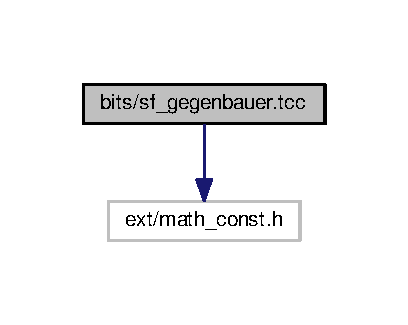
\includegraphics[width=350pt]{sf__gegenbauer_8tcc__incl}
\end{center}
\end{figure}
\doxysubsection*{Namespaces}
\begin{DoxyCompactItemize}
\item 
 \mbox{\hyperlink{namespaceemsr}{emsr}}
\item 
 \mbox{\hyperlink{namespaceemsr_1_1detail}{emsr\+::detail}}
\end{DoxyCompactItemize}
\doxysubsection*{Macros}
\begin{DoxyCompactItemize}
\item 
\#define \mbox{\hyperlink{sf__gegenbauer_8tcc_affeb207cda2f00080a1d0aa01f614339}{SF\+\_\+\+GEGENBAUER\+\_\+\+TCC}}~1
\end{DoxyCompactItemize}
\doxysubsection*{Functions}
\begin{DoxyCompactItemize}
\item 
{\footnotesize template$<$typename Tp $>$ }\\\mbox{\hyperlink{structemsr_1_1gegenbauer__t}{emsr\+::gegenbauer\+\_\+t}}$<$ Tp $>$ \mbox{\hyperlink{namespaceemsr_1_1detail_a50ca755c0c62879bde9a00ed145e60ca}{emsr\+::detail\+::gegenbauer\+\_\+recur}} (unsigned int n, Tp lambda, Tp x)
\item 
{\footnotesize template$<$typename Tp $>$ }\\std\+::vector$<$ emsr\+::\+Quadrature\+Point$<$ Tp $>$ $>$ \mbox{\hyperlink{namespaceemsr_1_1detail_a65f31111f8db58d173ea51bdd64461c4}{emsr\+::detail\+::gegenbauer\+\_\+zeros}} (unsigned int n, Tp lambda)
\end{DoxyCompactItemize}


\doxysubsection{Macro Definition Documentation}
\mbox{\Hypertarget{sf__gegenbauer_8tcc_affeb207cda2f00080a1d0aa01f614339}\label{sf__gegenbauer_8tcc_affeb207cda2f00080a1d0aa01f614339}} 
\index{sf\_gegenbauer.tcc@{sf\_gegenbauer.tcc}!SF\_GEGENBAUER\_TCC@{SF\_GEGENBAUER\_TCC}}
\index{SF\_GEGENBAUER\_TCC@{SF\_GEGENBAUER\_TCC}!sf\_gegenbauer.tcc@{sf\_gegenbauer.tcc}}
\doxysubsubsection{\texorpdfstring{SF\_GEGENBAUER\_TCC}{SF\_GEGENBAUER\_TCC}}
{\footnotesize\ttfamily \#define SF\+\_\+\+GEGENBAUER\+\_\+\+TCC~1}



Definition at line 30 of file sf\+\_\+gegenbauer.\+tcc.


\hypertarget{sf__hankel_8tcc}{}\section{bits/sf\+\_\+hankel.tcc File Reference}
\label{sf__hankel_8tcc}\index{bits/sf\+\_\+hankel.\+tcc@{bits/sf\+\_\+hankel.\+tcc}}
{\ttfamily \#include $<$complex$>$}\\*
{\ttfamily \#include $<$limits$>$}\\*
{\ttfamily \#include $<$vector$>$}\\*
{\ttfamily \#include $<$bits/complex\+\_\+util.\+h$>$}\\*
Include dependency graph for sf\+\_\+hankel.\+tcc\+:
\nopagebreak
\begin{figure}[H]
\begin{center}
\leavevmode
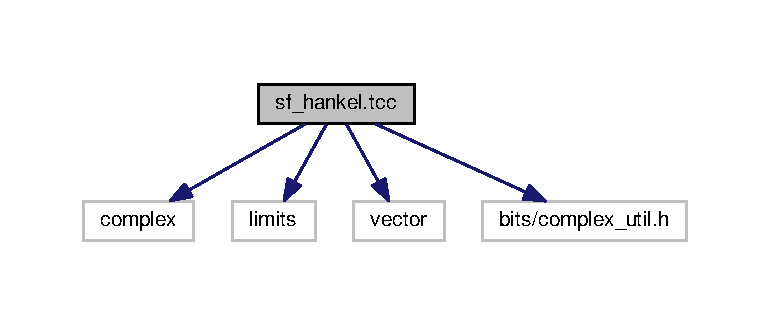
\includegraphics[width=350pt]{sf__hankel_8tcc__incl}
\end{center}
\end{figure}
This graph shows which files directly or indirectly include this file\+:
\nopagebreak
\begin{figure}[H]
\begin{center}
\leavevmode
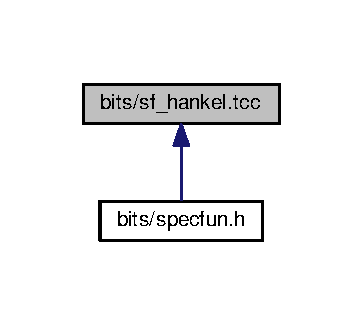
\includegraphics[width=174pt]{sf__hankel_8tcc__dep__incl}
\end{center}
\end{figure}
\subsection*{Namespaces}
\begin{DoxyCompactItemize}
\item 
 \hyperlink{namespacestd}{std}
\item 
 \hyperlink{namespacestd_1_1____detail}{std\+::\+\_\+\+\_\+detail}
\end{DoxyCompactItemize}
\subsection*{Macros}
\begin{DoxyCompactItemize}
\item 
\#define \hyperlink{sf__hankel_8tcc_add70af0902438b1aad02be015e5b9375}{\+\_\+\+G\+L\+I\+B\+C\+X\+X\+\_\+\+B\+I\+T\+S\+\_\+\+S\+F\+\_\+\+H\+A\+N\+K\+E\+L\+\_\+\+T\+CC}~1
\end{DoxyCompactItemize}
\subsection*{Functions}
\begin{DoxyCompactItemize}
\item 
{\footnotesize template$<$typename \+\_\+\+Tp $>$ }\\void \hyperlink{namespacestd_1_1____detail_a2473fe60310e9480137e3b66d3944f15}{std\+::\+\_\+\+\_\+detail\+::\+\_\+\+\_\+airy\+\_\+arg} (std\+::complex$<$ \+\_\+\+Tp $>$ \+\_\+\+\_\+num2d3, std\+::complex$<$ \+\_\+\+Tp $>$ \+\_\+\+\_\+zeta, std\+::complex$<$ \+\_\+\+Tp $>$ \&\+\_\+\+\_\+argp, std\+::complex$<$ \+\_\+\+Tp $>$ \&\+\_\+\+\_\+argm)
\begin{DoxyCompactList}\small\item\em Compute the arguments for the Airy function evaluations carefully to prevent premature overflow. Note that the major work here is in {\ttfamily safe\+\_\+div}. A faster, but less safe implementation can be obtained without use of safe\+\_\+div. \end{DoxyCompactList}\item 
{\footnotesize template$<$typename \+\_\+\+Tp $>$ }\\std\+::complex$<$ \+\_\+\+Tp $>$ \hyperlink{namespacestd_1_1____detail_ac4cff6a34fbd90932b47ecdb2445dee2}{std\+::\+\_\+\+\_\+detail\+::\+\_\+\+\_\+cyl\+\_\+bessel} (std\+::complex$<$ \+\_\+\+Tp $>$ \+\_\+\+\_\+nu, std\+::complex$<$ \+\_\+\+Tp $>$ \+\_\+\+\_\+z)
\begin{DoxyCompactList}\small\item\em Return the complex cylindrical Bessel function. \end{DoxyCompactList}\item 
{\footnotesize template$<$typename \+\_\+\+Tp $>$ }\\std\+::complex$<$ \+\_\+\+Tp $>$ \hyperlink{namespacestd_1_1____detail_a9904b6007ef78ef777ac8345f6e47960}{std\+::\+\_\+\+\_\+detail\+::\+\_\+\+\_\+cyl\+\_\+hankel\+\_\+1} (std\+::complex$<$ \+\_\+\+Tp $>$ \+\_\+\+\_\+nu, std\+::complex$<$ \+\_\+\+Tp $>$ \+\_\+\+\_\+z)
\begin{DoxyCompactList}\small\item\em Return the complex cylindrical Hankel function of the first kind. \end{DoxyCompactList}\item 
{\footnotesize template$<$typename \+\_\+\+Tp $>$ }\\std\+::complex$<$ \+\_\+\+Tp $>$ \hyperlink{namespacestd_1_1____detail_a3a8bdfd85729c705dec2586dfa5b275b}{std\+::\+\_\+\+\_\+detail\+::\+\_\+\+\_\+cyl\+\_\+hankel\+\_\+2} (std\+::complex$<$ \+\_\+\+Tp $>$ \+\_\+\+\_\+nu, std\+::complex$<$ \+\_\+\+Tp $>$ \+\_\+\+\_\+z)
\begin{DoxyCompactList}\small\item\em Return the complex cylindrical Hankel function of the second kind. \end{DoxyCompactList}\item 
{\footnotesize template$<$typename \+\_\+\+Tp $>$ }\\std\+::complex$<$ \+\_\+\+Tp $>$ \hyperlink{namespacestd_1_1____detail_ac73a4e3b8ac311760c998277aadb0fcb}{std\+::\+\_\+\+\_\+detail\+::\+\_\+\+\_\+cyl\+\_\+neumann} (std\+::complex$<$ \+\_\+\+Tp $>$ \+\_\+\+\_\+nu, std\+::complex$<$ \+\_\+\+Tp $>$ \+\_\+\+\_\+z)
\begin{DoxyCompactList}\small\item\em Return the complex cylindrical Neumann function. \end{DoxyCompactList}\item 
{\footnotesize template$<$typename \+\_\+\+Tp $>$ }\\void \hyperlink{namespacestd_1_1____detail_a3212c0a136417e862f2ed8e9684e053c}{std\+::\+\_\+\+\_\+detail\+::\+\_\+\+\_\+debye\+\_\+region} (std\+::complex$<$ \+\_\+\+Tp $>$ \+\_\+\+\_\+alpha, int \&\+\_\+\+\_\+indexr, char \&\+\_\+\+\_\+aorb)
\item 
{\footnotesize template$<$typename \+\_\+\+Tp $>$ }\\void \hyperlink{namespacestd_1_1____detail_a55f221be4308a6e366968d5cf3b840c2}{std\+::\+\_\+\+\_\+detail\+::\+\_\+\+\_\+hankel} (std\+::complex$<$ \+\_\+\+Tp $>$ \+\_\+\+\_\+nu, std\+::complex$<$ \+\_\+\+Tp $>$ \+\_\+\+\_\+z, std\+::complex$<$ \+\_\+\+Tp $>$ \&\+\_\+\+H1, std\+::complex$<$ \+\_\+\+Tp $>$ \&\+\_\+\+H2, std\+::complex$<$ \+\_\+\+Tp $>$ \&\+\_\+\+H1p, std\+::complex$<$ \+\_\+\+Tp $>$ \&\+\_\+\+H2p)
\item 
{\footnotesize template$<$typename \+\_\+\+Tp $>$ }\\void \hyperlink{namespacestd_1_1____detail_a4d1fa9f2ae57056ac102a33c2ddbe9c3}{std\+::\+\_\+\+\_\+detail\+::\+\_\+\+\_\+hankel\+\_\+debye} (std\+::complex$<$ \+\_\+\+Tp $>$ \+\_\+\+\_\+nu, std\+::complex$<$ \+\_\+\+Tp $>$ \+\_\+\+\_\+z, std\+::complex$<$ \+\_\+\+Tp $>$ \+\_\+\+\_\+alpha, int \+\_\+\+\_\+indexr, char \&\+\_\+\+\_\+aorb, int \&\+\_\+\+\_\+morn, std\+::complex$<$ \+\_\+\+Tp $>$ \&\+\_\+\+H1, std\+::complex$<$ \+\_\+\+Tp $>$ \&\+\_\+\+H2, std\+::complex$<$ \+\_\+\+Tp $>$ \&\+\_\+\+H1p, std\+::complex$<$ \+\_\+\+Tp $>$ \&\+\_\+\+H2p)
\item 
{\footnotesize template$<$typename \+\_\+\+Tp $>$ }\\void \hyperlink{namespacestd_1_1____detail_aff42671a79cd3852a57752f79c82f8da}{std\+::\+\_\+\+\_\+detail\+::\+\_\+\+\_\+hankel\+\_\+params} (std\+::complex$<$ \+\_\+\+Tp $>$ \+\_\+\+\_\+nu, std\+::complex$<$ \+\_\+\+Tp $>$ \+\_\+\+\_\+zhat, std\+::complex$<$ \+\_\+\+Tp $>$ \&\+\_\+\+\_\+p, std\+::complex$<$ \+\_\+\+Tp $>$ \&\+\_\+\+\_\+p2, std\+::complex$<$ \+\_\+\+Tp $>$ \&\+\_\+\+\_\+nup2, std\+::complex$<$ \+\_\+\+Tp $>$ \&\+\_\+\+\_\+num2, std\+::complex$<$ \+\_\+\+Tp $>$ \&\+\_\+\+\_\+num1d3, std\+::complex$<$ \+\_\+\+Tp $>$ \&\+\_\+\+\_\+num2d3, std\+::complex$<$ \+\_\+\+Tp $>$ \&\+\_\+\+\_\+num4d3, std\+::complex$<$ \+\_\+\+Tp $>$ \&\+\_\+\+\_\+zeta, std\+::complex$<$ \+\_\+\+Tp $>$ \&\+\_\+\+\_\+zetaphf, std\+::complex$<$ \+\_\+\+Tp $>$ \&\+\_\+\+\_\+zetamhf, std\+::complex$<$ \+\_\+\+Tp $>$ \&\+\_\+\+\_\+zetam3hf, std\+::complex$<$ \+\_\+\+Tp $>$ \&\+\_\+\+\_\+zetrat)
\begin{DoxyCompactList}\small\item\em Compute parameters depending on z and nu that appear in the uniform asymptotic expansions of the Hankel functions and their derivatives, except the arguments to the Airy functions. \end{DoxyCompactList}\item 
{\footnotesize template$<$typename \+\_\+\+Tp $>$ }\\void \hyperlink{namespacestd_1_1____detail_aa8e4a43b14fa416b1aa40b80293b44c8}{std\+::\+\_\+\+\_\+detail\+::\+\_\+\+\_\+hankel\+\_\+uniform} (std\+::complex$<$ \+\_\+\+Tp $>$ \+\_\+\+\_\+nu, std\+::complex$<$ \+\_\+\+Tp $>$ \+\_\+\+\_\+z, std\+::complex$<$ \+\_\+\+Tp $>$ \&\+\_\+\+H1, std\+::complex$<$ \+\_\+\+Tp $>$ \&\+\_\+\+H2, std\+::complex$<$ \+\_\+\+Tp $>$ \&\+\_\+\+H1p, std\+::complex$<$ \+\_\+\+Tp $>$ \&\+\_\+\+H2p)
\begin{DoxyCompactList}\small\item\em This routine computes the uniform asymptotic approximations of the Hankel functions and their derivatives including a patch for the case when the order equals or nearly equals the argument. At such points, Olver\textquotesingle{}s expressions have zero denominators (and numerators) resulting in numerical problems. This routine averages results from four surrounding points in the complex plane to obtain the result in such cases. \end{DoxyCompactList}\item 
{\footnotesize template$<$typename \+\_\+\+Tp $>$ }\\void \hyperlink{namespacestd_1_1____detail_a50641f445329898a247143de5a52629f}{std\+::\+\_\+\+\_\+detail\+::\+\_\+\+\_\+hankel\+\_\+uniform\+\_\+olver} (std\+::complex$<$ \+\_\+\+Tp $>$ \+\_\+\+\_\+nu, std\+::complex$<$ \+\_\+\+Tp $>$ \+\_\+\+\_\+z, std\+::complex$<$ \+\_\+\+Tp $>$ \&\+\_\+\+H1, std\+::complex$<$ \+\_\+\+Tp $>$ \&\+\_\+\+H2, std\+::complex$<$ \+\_\+\+Tp $>$ \&\+\_\+\+H1p, std\+::complex$<$ \+\_\+\+Tp $>$ \&\+\_\+\+H2p)
\begin{DoxyCompactList}\small\item\em Compute approximate values for the Hankel functions of the first and second kinds using Olver\textquotesingle{}s uniform asymptotic expansion to of order {\ttfamily nu} along with their derivatives. \end{DoxyCompactList}\item 
{\footnotesize template$<$typename \+\_\+\+Tp $>$ }\\void \hyperlink{namespacestd_1_1____detail_a099751f2a153283d91f19d6efa52117a}{std\+::\+\_\+\+\_\+detail\+::\+\_\+\+\_\+hankel\+\_\+uniform\+\_\+outer} (std\+::complex$<$ \+\_\+\+Tp $>$ \+\_\+\+\_\+nu, std\+::complex$<$ \+\_\+\+Tp $>$ \+\_\+\+\_\+z, \+\_\+\+Tp \+\_\+\+\_\+eps, std\+::complex$<$ \+\_\+\+Tp $>$ \&\+\_\+\+\_\+zhat, std\+::complex$<$ \+\_\+\+Tp $>$ \&\+\_\+\+\_\+1dnsq, std\+::complex$<$ \+\_\+\+Tp $>$ \&\+\_\+\+\_\+num1d3, std\+::complex$<$ \+\_\+\+Tp $>$ \&\+\_\+\+\_\+num2d3, std\+::complex$<$ \+\_\+\+Tp $>$ \&\+\_\+\+\_\+p, std\+::complex$<$ \+\_\+\+Tp $>$ \&\+\_\+\+\_\+p2, std\+::complex$<$ \+\_\+\+Tp $>$ \&\+\_\+\+\_\+etm3h, std\+::complex$<$ \+\_\+\+Tp $>$ \&\+\_\+\+\_\+etrat, std\+::complex$<$ \+\_\+\+Tp $>$ \&\+\_\+\+Aip, std\+::complex$<$ \+\_\+\+Tp $>$ \&\+\_\+\+\_\+o4dp, std\+::complex$<$ \+\_\+\+Tp $>$ \&\+\_\+\+Aim, std\+::complex$<$ \+\_\+\+Tp $>$ \&\+\_\+\+\_\+o4dm, std\+::complex$<$ \+\_\+\+Tp $>$ \&\+\_\+\+\_\+od2p, std\+::complex$<$ \+\_\+\+Tp $>$ \&\+\_\+\+\_\+od0dp, std\+::complex$<$ \+\_\+\+Tp $>$ \&\+\_\+\+\_\+od2m, std\+::complex$<$ \+\_\+\+Tp $>$ \&\+\_\+\+\_\+od0dm)
\begin{DoxyCompactList}\small\item\em Compute outer factors and associated functions of {\ttfamily z} and {\ttfamily nu} appearing in Olver\textquotesingle{}s uniform asymptotic expansions of the Hankel functions of the first and second kinds and their derivatives. The various functions of z and nu returned by {\ttfamily hankel\+\_\+uniform\+\_\+outer} are available for use in computing further terms in the expansions. \end{DoxyCompactList}\item 
{\footnotesize template$<$typename \+\_\+\+Tp $>$ }\\void \hyperlink{namespacestd_1_1____detail_a561dc02bc44b2dba376d6047289563c7}{std\+::\+\_\+\+\_\+detail\+::\+\_\+\+\_\+hankel\+\_\+uniform\+\_\+sum} (std\+::complex$<$ \+\_\+\+Tp $>$ \+\_\+\+\_\+p, std\+::complex$<$ \+\_\+\+Tp $>$ \+\_\+\+\_\+p2, std\+::complex$<$ \+\_\+\+Tp $>$ \+\_\+\+\_\+num2, std\+::complex$<$ \+\_\+\+Tp $>$ \+\_\+\+\_\+zetam3hf, std\+::complex$<$ \+\_\+\+Tp $>$ \+\_\+\+Aip, std\+::complex$<$ \+\_\+\+Tp $>$ \+\_\+\+\_\+o4dp, std\+::complex$<$ \+\_\+\+Tp $>$ \+\_\+\+Aim, std\+::complex$<$ \+\_\+\+Tp $>$ \+\_\+\+\_\+o4dm, std\+::complex$<$ \+\_\+\+Tp $>$ \+\_\+\+\_\+od2p, std\+::complex$<$ \+\_\+\+Tp $>$ \+\_\+\+\_\+od0dp, std\+::complex$<$ \+\_\+\+Tp $>$ \+\_\+\+\_\+od2m, std\+::complex$<$ \+\_\+\+Tp $>$ \+\_\+\+\_\+od0dm, \+\_\+\+Tp \+\_\+\+\_\+eps, std\+::complex$<$ \+\_\+\+Tp $>$ \&\+\_\+\+H1sum, std\+::complex$<$ \+\_\+\+Tp $>$ \&\+\_\+\+H1psum, std\+::complex$<$ \+\_\+\+Tp $>$ \&\+\_\+\+H2sum, std\+::complex$<$ \+\_\+\+Tp $>$ \&\+\_\+\+H2psum)
\begin{DoxyCompactList}\small\item\em Compute the sums in appropriate linear combinations appearing in Olver\textquotesingle{}s uniform asymptotic expansions for the Hankel functions of the first and second kinds and their derivatives, using up to nterms (less than 5) to achieve relative error {\ttfamily eps}. \end{DoxyCompactList}\item 
{\footnotesize template$<$typename \+\_\+\+Tp $>$ }\\std\+::complex$<$ \+\_\+\+Tp $>$ \hyperlink{namespacestd_1_1____detail_a28646bd01903e6da9871069a9363c593}{std\+::\+\_\+\+\_\+detail\+::\+\_\+\+\_\+sph\+\_\+bessel} (unsigned int \+\_\+\+\_\+n, std\+::complex$<$ \+\_\+\+Tp $>$ \+\_\+\+\_\+z)
\begin{DoxyCompactList}\small\item\em Return the complex spherical Bessel function. \end{DoxyCompactList}\item 
{\footnotesize template$<$typename \+\_\+\+Tp $>$ }\\void \hyperlink{namespacestd_1_1____detail_ae666168f9ede5a09dbae92598b7b14e4}{std\+::\+\_\+\+\_\+detail\+::\+\_\+\+\_\+sph\+\_\+hankel} (unsigned int \+\_\+\+\_\+n, std\+::complex$<$ \+\_\+\+Tp $>$ \+\_\+\+\_\+z, std\+::complex$<$ \+\_\+\+Tp $>$ \&\+\_\+\+H1, std\+::complex$<$ \+\_\+\+Tp $>$ \&\+\_\+\+H1p, std\+::complex$<$ \+\_\+\+Tp $>$ \&\+\_\+\+H2, std\+::complex$<$ \+\_\+\+Tp $>$ \&\+\_\+\+H2p)
\begin{DoxyCompactList}\small\item\em Helper to compute complex spherical Hankel functions and their derivatives. \end{DoxyCompactList}\item 
{\footnotesize template$<$typename \+\_\+\+Tp $>$ }\\std\+::complex$<$ \+\_\+\+Tp $>$ \hyperlink{namespacestd_1_1____detail_a887838c407a7cdb7c4ee145a18d2aa12}{std\+::\+\_\+\+\_\+detail\+::\+\_\+\+\_\+sph\+\_\+hankel\+\_\+1} (unsigned int \+\_\+\+\_\+n, std\+::complex$<$ \+\_\+\+Tp $>$ \+\_\+\+\_\+z)
\begin{DoxyCompactList}\small\item\em Return the complex spherical Hankel function of the first kind. \end{DoxyCompactList}\item 
{\footnotesize template$<$typename \+\_\+\+Tp $>$ }\\std\+::complex$<$ \+\_\+\+Tp $>$ \hyperlink{namespacestd_1_1____detail_ade83ff0131b8880428cbd58028d89bc5}{std\+::\+\_\+\+\_\+detail\+::\+\_\+\+\_\+sph\+\_\+hankel\+\_\+2} (unsigned int \+\_\+\+\_\+n, std\+::complex$<$ \+\_\+\+Tp $>$ \+\_\+\+\_\+z)
\begin{DoxyCompactList}\small\item\em Return the complex spherical Hankel function of the second kind. \end{DoxyCompactList}\item 
{\footnotesize template$<$typename \+\_\+\+Tp $>$ }\\std\+::complex$<$ \+\_\+\+Tp $>$ \hyperlink{namespacestd_1_1____detail_ac72e28d4d5fb8b0ffa033b9a47b67a8e}{std\+::\+\_\+\+\_\+detail\+::\+\_\+\+\_\+sph\+\_\+neumann} (unsigned int \+\_\+\+\_\+n, std\+::complex$<$ \+\_\+\+Tp $>$ \+\_\+\+\_\+z)
\begin{DoxyCompactList}\small\item\em Return the complex spherical Neumann function. \end{DoxyCompactList}\end{DoxyCompactItemize}


\subsection{Detailed Description}
This is an internal header file, included by other library headers. You should not attempt to use it directly. 

\subsection{Macro Definition Documentation}
\index{sf\+\_\+hankel.\+tcc@{sf\+\_\+hankel.\+tcc}!\+\_\+\+G\+L\+I\+B\+C\+X\+X\+\_\+\+B\+I\+T\+S\+\_\+\+S\+F\+\_\+\+H\+A\+N\+K\+E\+L\+\_\+\+T\+CC@{\+\_\+\+G\+L\+I\+B\+C\+X\+X\+\_\+\+B\+I\+T\+S\+\_\+\+S\+F\+\_\+\+H\+A\+N\+K\+E\+L\+\_\+\+T\+CC}}
\index{\+\_\+\+G\+L\+I\+B\+C\+X\+X\+\_\+\+B\+I\+T\+S\+\_\+\+S\+F\+\_\+\+H\+A\+N\+K\+E\+L\+\_\+\+T\+CC@{\+\_\+\+G\+L\+I\+B\+C\+X\+X\+\_\+\+B\+I\+T\+S\+\_\+\+S\+F\+\_\+\+H\+A\+N\+K\+E\+L\+\_\+\+T\+CC}!sf\+\_\+hankel.\+tcc@{sf\+\_\+hankel.\+tcc}}
\subsubsection[{\texorpdfstring{\+\_\+\+G\+L\+I\+B\+C\+X\+X\+\_\+\+B\+I\+T\+S\+\_\+\+S\+F\+\_\+\+H\+A\+N\+K\+E\+L\+\_\+\+T\+CC}{_GLIBCXX_BITS_SF_HANKEL_TCC}}]{\setlength{\rightskip}{0pt plus 5cm}\#define \+\_\+\+G\+L\+I\+B\+C\+X\+X\+\_\+\+B\+I\+T\+S\+\_\+\+S\+F\+\_\+\+H\+A\+N\+K\+E\+L\+\_\+\+T\+CC~1}\hypertarget{sf__hankel_8tcc_add70af0902438b1aad02be015e5b9375}{}\label{sf__hankel_8tcc_add70af0902438b1aad02be015e5b9375}


Definition at line 31 of file sf\+\_\+hankel.\+tcc.


\hypertarget{sf__hermite_8tcc}{}\section{sf\+\_\+hermite.\+tcc File Reference}
\label{sf__hermite_8tcc}\index{sf\+\_\+hermite.\+tcc@{sf\+\_\+hermite.\+tcc}}
{\ttfamily \#include $<$ext/math\+\_\+const.\+h$>$}\\*
Include dependency graph for sf\+\_\+hermite.\+tcc\+:
\nopagebreak
\begin{figure}[H]
\begin{center}
\leavevmode
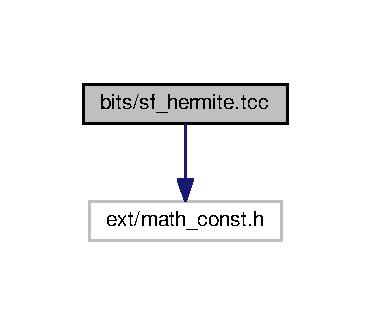
\includegraphics[width=172pt]{sf__hermite_8tcc__incl}
\end{center}
\end{figure}
\subsection*{Namespaces}
\begin{DoxyCompactItemize}
\item 
 \hyperlink{namespacestd}{std}
\item 
 \hyperlink{namespacestd_1_1____detail}{std\+::\+\_\+\+\_\+detail}
\end{DoxyCompactItemize}
\subsection*{Macros}
\begin{DoxyCompactItemize}
\item 
\#define \hyperlink{sf__hermite_8tcc_a0f8ec646afa7a1f2821820df783ca594}{\+\_\+\+G\+L\+I\+B\+C\+X\+X\+\_\+\+B\+I\+T\+S\+\_\+\+S\+F\+\_\+\+H\+E\+R\+M\+I\+T\+E\+\_\+\+T\+C\+C}~1
\end{DoxyCompactItemize}
\subsection*{Functions}
\begin{DoxyCompactItemize}
\item 
{\footnotesize template$<$typename \+\_\+\+Tp $>$ }\\\+\_\+\+Tp \hyperlink{namespacestd_1_1____detail_aca2f5400ce1d8ee26b9e0e9da74bda2c}{std\+::\+\_\+\+\_\+detail\+::\+\_\+\+\_\+poly\+\_\+hermite} (unsigned int \+\_\+\+\_\+n, \+\_\+\+Tp \+\_\+\+\_\+x)
\begin{DoxyCompactList}\small\item\em This routine returns the Hermite polynomial of order n\+: $ H_n(x) $. \end{DoxyCompactList}\item 
{\footnotesize template$<$typename \+\_\+\+Tp $>$ }\\\+\_\+\+Tp \hyperlink{namespacestd_1_1____detail_a34d8e6d2be42c2e9abb21a3090725912}{std\+::\+\_\+\+\_\+detail\+::\+\_\+\+\_\+poly\+\_\+hermite\+\_\+asymp} (unsigned int \+\_\+\+\_\+n, \+\_\+\+Tp \+\_\+\+\_\+x)
\begin{DoxyCompactList}\small\item\em This routine returns the Hermite polynomial of large order n\+: $ H_n(x) $. We assume here that x $>$= 0. \end{DoxyCompactList}\item 
{\footnotesize template$<$typename \+\_\+\+Tp $>$ }\\\+\_\+\+Tp \hyperlink{namespacestd_1_1____detail_a4dbbb56aec75c28da046df01112ba2d0}{std\+::\+\_\+\+\_\+detail\+::\+\_\+\+\_\+poly\+\_\+hermite\+\_\+recursion} (unsigned int \+\_\+\+\_\+n, \+\_\+\+Tp \+\_\+\+\_\+x)
\begin{DoxyCompactList}\small\item\em This routine returns the Hermite polynomial of order n\+: $ H_n(x) $ by recursion on n. \end{DoxyCompactList}\end{DoxyCompactItemize}


\subsection{Macro Definition Documentation}
\hypertarget{sf__hermite_8tcc_a0f8ec646afa7a1f2821820df783ca594}{}\index{sf\+\_\+hermite.\+tcc@{sf\+\_\+hermite.\+tcc}!\+\_\+\+G\+L\+I\+B\+C\+X\+X\+\_\+\+B\+I\+T\+S\+\_\+\+S\+F\+\_\+\+H\+E\+R\+M\+I\+T\+E\+\_\+\+T\+C\+C@{\+\_\+\+G\+L\+I\+B\+C\+X\+X\+\_\+\+B\+I\+T\+S\+\_\+\+S\+F\+\_\+\+H\+E\+R\+M\+I\+T\+E\+\_\+\+T\+C\+C}}
\index{\+\_\+\+G\+L\+I\+B\+C\+X\+X\+\_\+\+B\+I\+T\+S\+\_\+\+S\+F\+\_\+\+H\+E\+R\+M\+I\+T\+E\+\_\+\+T\+C\+C@{\+\_\+\+G\+L\+I\+B\+C\+X\+X\+\_\+\+B\+I\+T\+S\+\_\+\+S\+F\+\_\+\+H\+E\+R\+M\+I\+T\+E\+\_\+\+T\+C\+C}!sf\+\_\+hermite.\+tcc@{sf\+\_\+hermite.\+tcc}}
\subsubsection[{\+\_\+\+G\+L\+I\+B\+C\+X\+X\+\_\+\+B\+I\+T\+S\+\_\+\+S\+F\+\_\+\+H\+E\+R\+M\+I\+T\+E\+\_\+\+T\+C\+C}]{\setlength{\rightskip}{0pt plus 5cm}\#define \+\_\+\+G\+L\+I\+B\+C\+X\+X\+\_\+\+B\+I\+T\+S\+\_\+\+S\+F\+\_\+\+H\+E\+R\+M\+I\+T\+E\+\_\+\+T\+C\+C~1}\label{sf__hermite_8tcc_a0f8ec646afa7a1f2821820df783ca594}


Definition at line 42 of file sf\+\_\+hermite.\+tcc.


\hypertarget{sf__hydrogen_8tcc}{}\section{bits/sf\+\_\+hydrogen.tcc File Reference}
\label{sf__hydrogen_8tcc}\index{bits/sf\+\_\+hydrogen.\+tcc@{bits/sf\+\_\+hydrogen.\+tcc}}
This graph shows which files directly or indirectly include this file\+:
\nopagebreak
\begin{figure}[H]
\begin{center}
\leavevmode
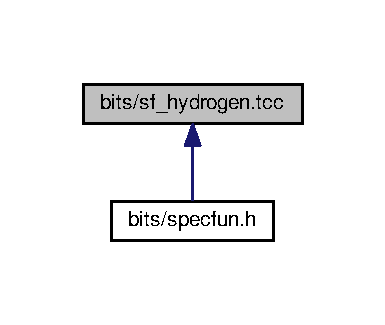
\includegraphics[width=185pt]{sf__hydrogen_8tcc__dep__incl}
\end{center}
\end{figure}
\subsection*{Namespaces}
\begin{DoxyCompactItemize}
\item 
 \hyperlink{namespacestd}{std}
\item 
 \hyperlink{namespacestd_1_1____detail}{std\+::\+\_\+\+\_\+detail}
\end{DoxyCompactItemize}
\subsection*{Macros}
\begin{DoxyCompactItemize}
\item 
\#define \hyperlink{sf__hydrogen_8tcc_af6b60d2402ae885b7f3ef4519fb65ed9}{\+\_\+\+G\+L\+I\+B\+C\+X\+X\+\_\+\+B\+I\+T\+S\+\_\+\+S\+F\+\_\+\+H\+Y\+D\+R\+O\+G\+E\+N\+\_\+\+T\+CC}~1
\end{DoxyCompactItemize}
\subsection*{Functions}
\begin{DoxyCompactItemize}
\item 
{\footnotesize template$<$typename \+\_\+\+Tp $>$ }\\std\+::complex$<$ \+\_\+\+Tp $>$ \hyperlink{namespacestd_1_1____detail_af8bd1ad6980e19dce3ee9eb518bc90fa}{std\+::\+\_\+\+\_\+detail\+::\+\_\+\+\_\+hydrogen} (const unsigned int \+\_\+\+\_\+n, const unsigned int \+\_\+\+\_\+l, const unsigned int \+\_\+\+\_\+m, const \+\_\+\+Tp \+\_\+Z, const \+\_\+\+Tp \+\_\+\+\_\+r, const \+\_\+\+Tp \+\_\+\+\_\+theta, const \+\_\+\+Tp \+\_\+\+\_\+phi)
\end{DoxyCompactItemize}


\subsection{Detailed Description}
This is an internal header file, included by other library headers. You should not attempt to use it directly. 

\subsection{Macro Definition Documentation}
\index{sf\+\_\+hydrogen.\+tcc@{sf\+\_\+hydrogen.\+tcc}!\+\_\+\+G\+L\+I\+B\+C\+X\+X\+\_\+\+B\+I\+T\+S\+\_\+\+S\+F\+\_\+\+H\+Y\+D\+R\+O\+G\+E\+N\+\_\+\+T\+CC@{\+\_\+\+G\+L\+I\+B\+C\+X\+X\+\_\+\+B\+I\+T\+S\+\_\+\+S\+F\+\_\+\+H\+Y\+D\+R\+O\+G\+E\+N\+\_\+\+T\+CC}}
\index{\+\_\+\+G\+L\+I\+B\+C\+X\+X\+\_\+\+B\+I\+T\+S\+\_\+\+S\+F\+\_\+\+H\+Y\+D\+R\+O\+G\+E\+N\+\_\+\+T\+CC@{\+\_\+\+G\+L\+I\+B\+C\+X\+X\+\_\+\+B\+I\+T\+S\+\_\+\+S\+F\+\_\+\+H\+Y\+D\+R\+O\+G\+E\+N\+\_\+\+T\+CC}!sf\+\_\+hydrogen.\+tcc@{sf\+\_\+hydrogen.\+tcc}}
\subsubsection[{\texorpdfstring{\+\_\+\+G\+L\+I\+B\+C\+X\+X\+\_\+\+B\+I\+T\+S\+\_\+\+S\+F\+\_\+\+H\+Y\+D\+R\+O\+G\+E\+N\+\_\+\+T\+CC}{_GLIBCXX_BITS_SF_HYDROGEN_TCC}}]{\setlength{\rightskip}{0pt plus 5cm}\#define \+\_\+\+G\+L\+I\+B\+C\+X\+X\+\_\+\+B\+I\+T\+S\+\_\+\+S\+F\+\_\+\+H\+Y\+D\+R\+O\+G\+E\+N\+\_\+\+T\+CC~1}\hypertarget{sf__hydrogen_8tcc_af6b60d2402ae885b7f3ef4519fb65ed9}{}\label{sf__hydrogen_8tcc_af6b60d2402ae885b7f3ef4519fb65ed9}


Definition at line 31 of file sf\+\_\+hydrogen.\+tcc.


\hypertarget{sf__hyperg_8tcc}{}\doxysection{cxx\+\_\+special\+\_\+functions/include/emsr/detail/sf\+\_\+hyperg.tcc File Reference}
\label{sf__hyperg_8tcc}\index{cxx\_special\_functions/include/emsr/detail/sf\_hyperg.tcc@{cxx\_special\_functions/include/emsr/detail/sf\_hyperg.tcc}}
{\ttfamily \#include $<$stdexcept$>$}\newline
{\ttfamily \#include $<$emsr/notsospecfun.\+h$>$}\newline
{\ttfamily \#include $<$emsr/numeric\+\_\+limits.\+h$>$}\newline
{\ttfamily \#include $<$emsr/math\+\_\+constants.\+h$>$}\newline
{\ttfamily \#include $<$emsr/math\+\_\+util.\+h$>$}\newline
{\ttfamily \#include $<$emsr/sf\+\_\+gamma.\+h$>$}\newline
Include dependency graph for sf\+\_\+hyperg.\+tcc\+:
\nopagebreak
\begin{figure}[H]
\begin{center}
\leavevmode
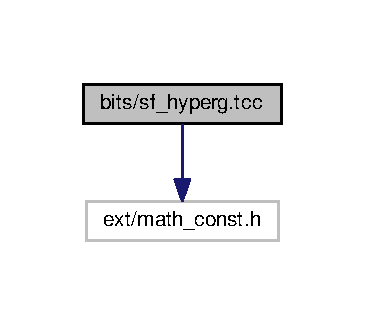
\includegraphics[width=350pt]{sf__hyperg_8tcc__incl}
\end{center}
\end{figure}
\doxysubsection*{Namespaces}
\begin{DoxyCompactItemize}
\item 
 \mbox{\hyperlink{namespaceemsr}{emsr}}
\item 
 \mbox{\hyperlink{namespaceemsr_1_1detail}{emsr\+::detail}}
\end{DoxyCompactItemize}
\doxysubsection*{Macros}
\begin{DoxyCompactItemize}
\item 
\#define \mbox{\hyperlink{sf__hyperg_8tcc_a4a4e391dacd901b1b5a2f8c4251af0b6}{SF\+\_\+\+HYPERG\+\_\+\+TCC}}~1
\end{DoxyCompactItemize}
\doxysubsection*{Functions}
\begin{DoxyCompactItemize}
\item 
{\footnotesize template$<$typename Tp $>$ }\\Tp \mbox{\hyperlink{namespaceemsr_1_1detail_a93b0db44829c28a42adf3800831aae68}{emsr\+::detail\+::conf\+\_\+hyperg}} (Tp a, Tp c, Tp x)
\begin{DoxyCompactList}\small\item\em Return the confluent hypergeometric function $ {}_1F_1(a;c;x) = M(a,c,x) $. \end{DoxyCompactList}\item 
{\footnotesize template$<$typename Tp $>$ }\\Tp \mbox{\hyperlink{namespaceemsr_1_1detail_a71735c35a77ac7a528c9a3218101de7c}{emsr\+::detail\+::conf\+\_\+hyperg\+\_\+lim}} (Tp c, Tp x)
\begin{DoxyCompactList}\small\item\em Return the confluent hypergeometric limit function $ {}_0F_1(-;c;x) $. \end{DoxyCompactList}\item 
{\footnotesize template$<$typename Tp $>$ }\\Tp \mbox{\hyperlink{namespaceemsr_1_1detail_ae77a326638bd76db826a9a4a3fc027db}{emsr\+::detail\+::conf\+\_\+hyperg\+\_\+lim\+\_\+series}} (Tp c, Tp x)
\begin{DoxyCompactList}\small\item\em This routine returns the confluent hypergeometric limit function by series expansion. \end{DoxyCompactList}\item 
{\footnotesize template$<$typename Tp $>$ }\\Tp \mbox{\hyperlink{namespaceemsr_1_1detail_a8b3296aad58701ec768b4e26442c5e4c}{emsr\+::detail\+::conf\+\_\+hyperg\+\_\+luke}} (Tp a, Tp c, Tp xin)
\begin{DoxyCompactList}\small\item\em Return the hypergeometric function $ {}_1F_1(a;c;x) $ by an iterative procedure described in Luke, Algorithms for the Computation of Mathematical Functions. \end{DoxyCompactList}\item 
{\footnotesize template$<$typename Tp $>$ }\\Tp \mbox{\hyperlink{namespaceemsr_1_1detail_a6730af49e014074c7703f6db7a616f6b}{emsr\+::detail\+::conf\+\_\+hyperg\+\_\+series}} (Tp a, Tp c, Tp x)
\begin{DoxyCompactList}\small\item\em This routine returns the confluent hypergeometric function by series expansion. \end{DoxyCompactList}\item 
{\footnotesize template$<$typename Tp $>$ }\\Tp \mbox{\hyperlink{namespaceemsr_1_1detail_a534b5cb2286d57b0eaf375b5d70c9db1}{emsr\+::detail\+::hyperg}} (Tp a, Tp b, Tp c, Tp x)
\begin{DoxyCompactList}\small\item\em Return the hypergeometric function $ {}_2F_1(a,b;c;x) $. \end{DoxyCompactList}\item 
{\footnotesize template$<$typename Tp $>$ }\\Tp \mbox{\hyperlink{namespaceemsr_1_1detail_a3ef3127649e7814975106f8c9abbe3ee}{emsr\+::detail\+::hyperg\+\_\+luke}} (Tp a, Tp b, Tp c, Tp xin)
\begin{DoxyCompactList}\small\item\em Return the hypergeometric function $ {}_2F_1(a,b;c;x) $ by an iterative procedure described in Luke, Algorithms for the Computation of Mathematical Functions. \end{DoxyCompactList}\item 
{\footnotesize template$<$typename Tp $>$ }\\Tp \mbox{\hyperlink{namespaceemsr_1_1detail_ade5de4140aef8537d722ce0b33b1cc11}{emsr\+::detail\+::hyperg\+\_\+recur}} (int m, Tp b, Tp c, Tp x)
\begin{DoxyCompactList}\small\item\em Return the hypergeometric polynomial $ {}_2F_1(-m,b;c;x) $ by Holm recursion. \end{DoxyCompactList}\item 
{\footnotesize template$<$typename Tp $>$ }\\Tp \mbox{\hyperlink{namespaceemsr_1_1detail_acd1546d7f0871fb6a225faeff9204588}{emsr\+::detail\+::hyperg\+\_\+reflect}} (Tp a, Tp b, Tp c, Tp x)
\begin{DoxyCompactList}\small\item\em Return the hypergeometric function $ {}_2F_1(a,b;c;x) $ by the reflection formulae in Abramowitz \& Stegun formula 15.\+3.\+6 for d = c -\/ a -\/ b not integral and formula 15.\+3.\+11 for d = c -\/ a -\/ b integral. This assumes a, b, c != negative integer. \end{DoxyCompactList}\item 
{\footnotesize template$<$typename Tp $>$ }\\Tp \mbox{\hyperlink{namespaceemsr_1_1detail_a9e085acad3ec48ebb7bef692e6388ae7}{emsr\+::detail\+::hyperg\+\_\+series}} (Tp a, Tp b, Tp c, Tp x)
\begin{DoxyCompactList}\small\item\em Return the hypergeometric function $ {}_2F_1(a,b;c;x) $ by series expansion. \end{DoxyCompactList}\item 
{\footnotesize template$<$typename Tp $>$ }\\Tp \mbox{\hyperlink{namespaceemsr_1_1detail_acadc5c031a10a44c85af64dd4c555d70}{emsr\+::detail\+::tricomi\+\_\+u}} (Tp a, Tp c, Tp x)
\begin{DoxyCompactList}\small\item\em Return the Tricomi confluent hypergeometric function. \end{DoxyCompactList}\item 
{\footnotesize template$<$typename Tp $>$ }\\Tp \mbox{\hyperlink{namespaceemsr_1_1detail_a3bc67d9d78aa295fd783a1bde2e0297c}{emsr\+::detail\+::tricomi\+\_\+u\+\_\+naive}} (Tp a, Tp c, Tp x)
\begin{DoxyCompactList}\small\item\em Return the Tricomi confluent hypergeometric function. \end{DoxyCompactList}\end{DoxyCompactItemize}


\doxysubsection{Macro Definition Documentation}
\mbox{\Hypertarget{sf__hyperg_8tcc_a4a4e391dacd901b1b5a2f8c4251af0b6}\label{sf__hyperg_8tcc_a4a4e391dacd901b1b5a2f8c4251af0b6}} 
\index{sf\_hyperg.tcc@{sf\_hyperg.tcc}!SF\_HYPERG\_TCC@{SF\_HYPERG\_TCC}}
\index{SF\_HYPERG\_TCC@{SF\_HYPERG\_TCC}!sf\_hyperg.tcc@{sf\_hyperg.tcc}}
\doxysubsubsection{\texorpdfstring{SF\_HYPERG\_TCC}{SF\_HYPERG\_TCC}}
{\footnotesize\ttfamily \#define SF\+\_\+\+HYPERG\+\_\+\+TCC~1}



Definition at line 43 of file sf\+\_\+hyperg.\+tcc.


\hypertarget{sf__hypint_8tcc}{}\section{sf\+\_\+hypint.\+tcc File Reference}
\label{sf__hypint_8tcc}\index{sf\+\_\+hypint.\+tcc@{sf\+\_\+hypint.\+tcc}}
{\ttfamily \#include $<$ext/math\+\_\+const.\+h$>$}\\*
Include dependency graph for sf\+\_\+hypint.\+tcc\+:\nopagebreak
\begin{figure}[H]
\begin{center}
\leavevmode
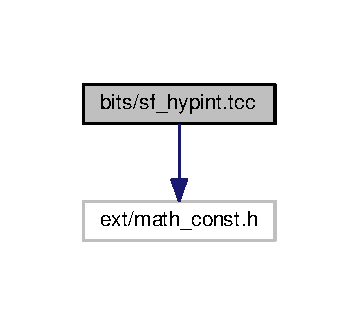
\includegraphics[width=172pt]{sf__hypint_8tcc__incl}
\end{center}
\end{figure}
\subsection*{Namespaces}
\begin{DoxyCompactItemize}
\item 
 \hyperlink{namespacestd}{std}
\item 
 \hyperlink{namespacestd_1_1____detail}{std\+::\+\_\+\+\_\+detail}
\end{DoxyCompactItemize}
\subsection*{Macros}
\begin{DoxyCompactItemize}
\item 
\#define \hyperlink{sf__hypint_8tcc_acf643c2e2a7b3fab7ab4a8be18e29584}{\+\_\+\+G\+L\+I\+B\+C\+X\+X\+\_\+\+S\+F\+\_\+\+H\+Y\+P\+I\+N\+T\+\_\+\+T\+C\+C}~1
\end{DoxyCompactItemize}
\subsection*{Functions}
\begin{DoxyCompactItemize}
\item 
{\footnotesize template$<$typename \+\_\+\+Tp $>$ }\\std\+::pair$<$ \+\_\+\+Tp, \+\_\+\+Tp $>$ \hyperlink{namespacestd_1_1____detail_aa07abc4dac6cf589ccd12d3ce40277cf}{std\+::\+\_\+\+\_\+detail\+::\+\_\+\+\_\+chshint} (\+\_\+\+Tp \+\_\+\+\_\+x, \+\_\+\+Tp \&\+\_\+\+Chi, \+\_\+\+Tp \&\+\_\+\+Shi)
\begin{DoxyCompactList}\small\item\em This function returns the hyperbolic cosine $ Ci(x) $ and hyperbolic sine $ Si(x) $ integrals as a pair. \end{DoxyCompactList}\item 
{\footnotesize template$<$typename \+\_\+\+Tp $>$ }\\void \hyperlink{namespacestd_1_1____detail_a07da2303d36d77bfad393a7b8ebdf686}{std\+::\+\_\+\+\_\+detail\+::\+\_\+\+\_\+chshint\+\_\+cont\+\_\+frac} (\+\_\+\+Tp \+\_\+\+\_\+t, \+\_\+\+Tp \&\+\_\+\+Chi, \+\_\+\+Tp \&\+\_\+\+Shi)
\begin{DoxyCompactList}\small\item\em This function computes the hyperbolic cosine $ Chi(x) $ and hyperbolic sine $ Shi(x) $ integrals by continued fraction for positive argument. \end{DoxyCompactList}\item 
{\footnotesize template$<$typename \+\_\+\+Tp $>$ }\\void \hyperlink{namespacestd_1_1____detail_a16055b6e4baa35ffe5c6d9495d9d0158}{std\+::\+\_\+\+\_\+detail\+::\+\_\+\+\_\+chshint\+\_\+series} (\+\_\+\+Tp \+\_\+\+\_\+t, \+\_\+\+Tp \&\+\_\+\+Chi, \+\_\+\+Tp \&\+\_\+\+Shi)
\begin{DoxyCompactList}\small\item\em This function computes the hyperbolic cosine $ Chi(x) $ and hyperbolic sine $ Shi(x) $ integrals by series summation for positive argument. \end{DoxyCompactList}\end{DoxyCompactItemize}


\subsection{Macro Definition Documentation}
\hypertarget{sf__hypint_8tcc_acf643c2e2a7b3fab7ab4a8be18e29584}{}\index{sf\+\_\+hypint.\+tcc@{sf\+\_\+hypint.\+tcc}!\+\_\+\+G\+L\+I\+B\+C\+X\+X\+\_\+\+S\+F\+\_\+\+H\+Y\+P\+I\+N\+T\+\_\+\+T\+C\+C@{\+\_\+\+G\+L\+I\+B\+C\+X\+X\+\_\+\+S\+F\+\_\+\+H\+Y\+P\+I\+N\+T\+\_\+\+T\+C\+C}}
\index{\+\_\+\+G\+L\+I\+B\+C\+X\+X\+\_\+\+S\+F\+\_\+\+H\+Y\+P\+I\+N\+T\+\_\+\+T\+C\+C@{\+\_\+\+G\+L\+I\+B\+C\+X\+X\+\_\+\+S\+F\+\_\+\+H\+Y\+P\+I\+N\+T\+\_\+\+T\+C\+C}!sf\+\_\+hypint.\+tcc@{sf\+\_\+hypint.\+tcc}}
\subsubsection[{\+\_\+\+G\+L\+I\+B\+C\+X\+X\+\_\+\+S\+F\+\_\+\+H\+Y\+P\+I\+N\+T\+\_\+\+T\+C\+C}]{\setlength{\rightskip}{0pt plus 5cm}\#define \+\_\+\+G\+L\+I\+B\+C\+X\+X\+\_\+\+S\+F\+\_\+\+H\+Y\+P\+I\+N\+T\+\_\+\+T\+C\+C~1}\label{sf__hypint_8tcc_acf643c2e2a7b3fab7ab4a8be18e29584}


Definition at line 31 of file sf\+\_\+hypint.\+tcc.


\hypertarget{sf__jacobi_8tcc}{}\section{bits/sf\+\_\+jacobi.tcc File Reference}
\label{sf__jacobi_8tcc}\index{bits/sf\+\_\+jacobi.\+tcc@{bits/sf\+\_\+jacobi.\+tcc}}
{\ttfamily \#include $<$ext/math\+\_\+const.\+h$>$}\\*
Include dependency graph for sf\+\_\+jacobi.\+tcc\+:
\nopagebreak
\begin{figure}[H]
\begin{center}
\leavevmode
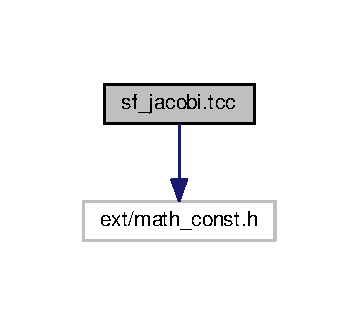
\includegraphics[width=172pt]{sf__jacobi_8tcc__incl}
\end{center}
\end{figure}
This graph shows which files directly or indirectly include this file\+:
\nopagebreak
\begin{figure}[H]
\begin{center}
\leavevmode
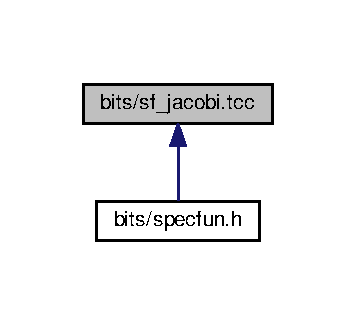
\includegraphics[width=171pt]{sf__jacobi_8tcc__dep__incl}
\end{center}
\end{figure}
\subsection*{Namespaces}
\begin{DoxyCompactItemize}
\item 
 \hyperlink{namespacestd}{std}
\item 
 \hyperlink{namespacestd_1_1____detail}{std\+::\+\_\+\+\_\+detail}
\end{DoxyCompactItemize}
\subsection*{Macros}
\begin{DoxyCompactItemize}
\item 
\#define \hyperlink{sf__jacobi_8tcc_aa88c9b1eaafd3bc961b110fcb09bbceb}{\+\_\+\+G\+L\+I\+B\+C\+X\+X\+\_\+\+B\+I\+T\+S\+\_\+\+S\+F\+\_\+\+J\+A\+C\+O\+B\+I\+\_\+\+T\+CC}~1
\end{DoxyCompactItemize}
\subsection*{Functions}
\begin{DoxyCompactItemize}
\item 
{\footnotesize template$<$typename \+\_\+\+Tp $>$ }\\\+\_\+\+Tp \hyperlink{namespacestd_1_1____detail_a7fcc47c397903ac177380517e94153c6}{std\+::\+\_\+\+\_\+detail\+::\+\_\+\+\_\+poly\+\_\+jacobi} (unsigned int \+\_\+\+\_\+n, \+\_\+\+Tp \+\_\+\+\_\+alpha, \+\_\+\+Tp \+\_\+\+\_\+beta, \+\_\+\+Tp \+\_\+\+\_\+x)
\item 
{\footnotesize template$<$typename \+\_\+\+Tp $>$ }\\\+\_\+\+Tp \hyperlink{namespacestd_1_1____detail_af325d47042bc9661bbde61b13f368fec}{std\+::\+\_\+\+\_\+detail\+::\+\_\+\+\_\+poly\+\_\+radial\+\_\+jacobi} (unsigned int \+\_\+\+\_\+n, unsigned int \+\_\+\+\_\+m, \+\_\+\+Tp \+\_\+\+\_\+rho)
\item 
{\footnotesize template$<$typename \+\_\+\+Tp $>$ }\\\+\_\+\+\_\+gnu\+\_\+cxx\+::\+\_\+\+\_\+promote\+\_\+fp\+\_\+t$<$ \+\_\+\+Tp $>$ \hyperlink{namespacestd_1_1____detail_aa09d6c12ea20927f2ea5f7a1ba2f8319}{std\+::\+\_\+\+\_\+detail\+::\+\_\+\+\_\+zernike} (unsigned int \+\_\+\+\_\+n, int \+\_\+\+\_\+m, \+\_\+\+Tp \+\_\+\+\_\+rho, \+\_\+\+Tp \+\_\+\+\_\+phi)
\end{DoxyCompactItemize}


\subsection{Detailed Description}
This is an internal header file, included by other library headers. Do not attempt to use it directly. Instead, include $<$cmath$>$. 

\subsection{Macro Definition Documentation}
\index{sf\+\_\+jacobi.\+tcc@{sf\+\_\+jacobi.\+tcc}!\+\_\+\+G\+L\+I\+B\+C\+X\+X\+\_\+\+B\+I\+T\+S\+\_\+\+S\+F\+\_\+\+J\+A\+C\+O\+B\+I\+\_\+\+T\+CC@{\+\_\+\+G\+L\+I\+B\+C\+X\+X\+\_\+\+B\+I\+T\+S\+\_\+\+S\+F\+\_\+\+J\+A\+C\+O\+B\+I\+\_\+\+T\+CC}}
\index{\+\_\+\+G\+L\+I\+B\+C\+X\+X\+\_\+\+B\+I\+T\+S\+\_\+\+S\+F\+\_\+\+J\+A\+C\+O\+B\+I\+\_\+\+T\+CC@{\+\_\+\+G\+L\+I\+B\+C\+X\+X\+\_\+\+B\+I\+T\+S\+\_\+\+S\+F\+\_\+\+J\+A\+C\+O\+B\+I\+\_\+\+T\+CC}!sf\+\_\+jacobi.\+tcc@{sf\+\_\+jacobi.\+tcc}}
\subsubsection[{\texorpdfstring{\+\_\+\+G\+L\+I\+B\+C\+X\+X\+\_\+\+B\+I\+T\+S\+\_\+\+S\+F\+\_\+\+J\+A\+C\+O\+B\+I\+\_\+\+T\+CC}{_GLIBCXX_BITS_SF_JACOBI_TCC}}]{\setlength{\rightskip}{0pt plus 5cm}\#define \+\_\+\+G\+L\+I\+B\+C\+X\+X\+\_\+\+B\+I\+T\+S\+\_\+\+S\+F\+\_\+\+J\+A\+C\+O\+B\+I\+\_\+\+T\+CC~1}\hypertarget{sf__jacobi_8tcc_aa88c9b1eaafd3bc961b110fcb09bbceb}{}\label{sf__jacobi_8tcc_aa88c9b1eaafd3bc961b110fcb09bbceb}


Definition at line 31 of file sf\+\_\+jacobi.\+tcc.


\hypertarget{sf__laguerre_8tcc}{}\section{sf\+\_\+laguerre.\+tcc File Reference}
\label{sf__laguerre_8tcc}\index{sf\+\_\+laguerre.\+tcc@{sf\+\_\+laguerre.\+tcc}}
{\ttfamily \#include $<$ext/math\+\_\+const.\+h$>$}\\*
Include dependency graph for sf\+\_\+laguerre.\+tcc\+:
\nopagebreak
\begin{figure}[H]
\begin{center}
\leavevmode
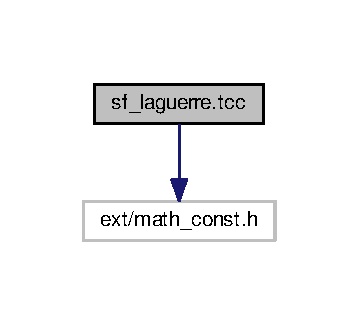
\includegraphics[width=172pt]{sf__laguerre_8tcc__incl}
\end{center}
\end{figure}
\subsection*{Namespaces}
\begin{DoxyCompactItemize}
\item 
 \hyperlink{namespacestd}{std}
\item 
 \hyperlink{namespacestd_1_1____detail}{std\+::\+\_\+\+\_\+detail}
\end{DoxyCompactItemize}
\subsection*{Macros}
\begin{DoxyCompactItemize}
\item 
\#define \hyperlink{sf__laguerre_8tcc_a6d5a7e97abaa68b4a97764d871fb5314}{\+\_\+\+G\+L\+I\+B\+C\+X\+X\+\_\+\+B\+I\+T\+S\+\_\+\+S\+F\+\_\+\+L\+A\+G\+U\+E\+R\+R\+E\+\_\+\+T\+C\+C}~1
\end{DoxyCompactItemize}
\subsection*{Functions}
\begin{DoxyCompactItemize}
\item 
{\footnotesize template$<$typename \+\_\+\+Tp $>$ }\\\+\_\+\+Tp \hyperlink{namespacestd_1_1____detail_a7d47c4512f7c6914f5504fde6ffa31fb}{std\+::\+\_\+\+\_\+detail\+::\+\_\+\+\_\+assoc\+\_\+laguerre} (unsigned int \+\_\+\+\_\+n, unsigned int \+\_\+\+\_\+m, \+\_\+\+Tp \+\_\+\+\_\+x)
\begin{DoxyCompactList}\small\item\em This routine returns the associated Laguerre polynomial of order n, degree m\+: $ L_n^m(x) $. \end{DoxyCompactList}\item 
{\footnotesize template$<$typename \+\_\+\+Tp $>$ }\\\+\_\+\+Tp \hyperlink{namespacestd_1_1____detail_aa714c4983a3cb7d9d18e0c2c5a8f6826}{std\+::\+\_\+\+\_\+detail\+::\+\_\+\+\_\+laguerre} (unsigned int \+\_\+\+\_\+n, \+\_\+\+Tp \+\_\+\+\_\+x)
\begin{DoxyCompactList}\small\item\em This routine returns the Laguerre polynomial of order n\+: $ L_n(x) $. \end{DoxyCompactList}\item 
{\footnotesize template$<$typename \+\_\+\+Tpa , typename \+\_\+\+Tp $>$ }\\\+\_\+\+Tp \hyperlink{namespacestd_1_1____detail_a76704115fd45b240802f4ccc433bb033}{std\+::\+\_\+\+\_\+detail\+::\+\_\+\+\_\+poly\+\_\+laguerre} (unsigned int \+\_\+\+\_\+n, \+\_\+\+Tpa \+\_\+\+\_\+alpha1, \+\_\+\+Tp \+\_\+\+\_\+x)
\begin{DoxyCompactList}\small\item\em This routine returns the associated Laguerre polynomial of order n, degree $ \alpha $\+: $ L_n^alpha(x) $. \end{DoxyCompactList}\item 
{\footnotesize template$<$typename \+\_\+\+Tpa , typename \+\_\+\+Tp $>$ }\\\+\_\+\+Tp \hyperlink{namespacestd_1_1____detail_a1c817d7f5df1147829ad745176325cd6}{std\+::\+\_\+\+\_\+detail\+::\+\_\+\+\_\+poly\+\_\+laguerre\+\_\+hyperg} (unsigned int \+\_\+\+\_\+n, \+\_\+\+Tpa \+\_\+\+\_\+alpha1, \+\_\+\+Tp \+\_\+\+\_\+x)
\begin{DoxyCompactList}\small\item\em Evaluate the polynomial based on the confluent hypergeometric function in a safe way, with no restriction on the arguments. \end{DoxyCompactList}\item 
{\footnotesize template$<$typename \+\_\+\+Tpa , typename \+\_\+\+Tp $>$ }\\\+\_\+\+Tp \hyperlink{namespacestd_1_1____detail_a1f9e78deb2bcc73511c77dcb1cdcf4c8}{std\+::\+\_\+\+\_\+detail\+::\+\_\+\+\_\+poly\+\_\+laguerre\+\_\+large\+\_\+n} (unsigned \+\_\+\+\_\+n, \+\_\+\+Tpa \+\_\+\+\_\+alpha1, \+\_\+\+Tp \+\_\+\+\_\+x)
\begin{DoxyCompactList}\small\item\em This routine returns the associated Laguerre polynomial of order $ n $, degree $ \alpha $ for large n. Abramowitz \& Stegun, 13.\+5.\+21. \end{DoxyCompactList}\item 
{\footnotesize template$<$typename \+\_\+\+Tpa , typename \+\_\+\+Tp $>$ }\\\+\_\+\+Tp \hyperlink{namespacestd_1_1____detail_a6d3a7499bd109d5c0ea01e85f3165730}{std\+::\+\_\+\+\_\+detail\+::\+\_\+\+\_\+poly\+\_\+laguerre\+\_\+recursion} (unsigned int \+\_\+\+\_\+n, \+\_\+\+Tpa \+\_\+\+\_\+alpha1, \+\_\+\+Tp \+\_\+\+\_\+x)
\begin{DoxyCompactList}\small\item\em This routine returns the associated Laguerre polynomial of order {\ttfamily n}, degree {\ttfamily $ \alpha $}\+: $ L_n^\alpha(x) $ by recursion. \end{DoxyCompactList}\end{DoxyCompactItemize}


\subsection{Macro Definition Documentation}
\hypertarget{sf__laguerre_8tcc_a6d5a7e97abaa68b4a97764d871fb5314}{}\index{sf\+\_\+laguerre.\+tcc@{sf\+\_\+laguerre.\+tcc}!\+\_\+\+G\+L\+I\+B\+C\+X\+X\+\_\+\+B\+I\+T\+S\+\_\+\+S\+F\+\_\+\+L\+A\+G\+U\+E\+R\+R\+E\+\_\+\+T\+C\+C@{\+\_\+\+G\+L\+I\+B\+C\+X\+X\+\_\+\+B\+I\+T\+S\+\_\+\+S\+F\+\_\+\+L\+A\+G\+U\+E\+R\+R\+E\+\_\+\+T\+C\+C}}
\index{\+\_\+\+G\+L\+I\+B\+C\+X\+X\+\_\+\+B\+I\+T\+S\+\_\+\+S\+F\+\_\+\+L\+A\+G\+U\+E\+R\+R\+E\+\_\+\+T\+C\+C@{\+\_\+\+G\+L\+I\+B\+C\+X\+X\+\_\+\+B\+I\+T\+S\+\_\+\+S\+F\+\_\+\+L\+A\+G\+U\+E\+R\+R\+E\+\_\+\+T\+C\+C}!sf\+\_\+laguerre.\+tcc@{sf\+\_\+laguerre.\+tcc}}
\subsubsection[{\+\_\+\+G\+L\+I\+B\+C\+X\+X\+\_\+\+B\+I\+T\+S\+\_\+\+S\+F\+\_\+\+L\+A\+G\+U\+E\+R\+R\+E\+\_\+\+T\+C\+C}]{\setlength{\rightskip}{0pt plus 5cm}\#define \+\_\+\+G\+L\+I\+B\+C\+X\+X\+\_\+\+B\+I\+T\+S\+\_\+\+S\+F\+\_\+\+L\+A\+G\+U\+E\+R\+R\+E\+\_\+\+T\+C\+C~1}\label{sf__laguerre_8tcc_a6d5a7e97abaa68b4a97764d871fb5314}


Definition at line 44 of file sf\+\_\+laguerre.\+tcc.


\hypertarget{sf__legendre_8tcc}{}\section{sf\+\_\+legendre.\+tcc File Reference}
\label{sf__legendre_8tcc}\index{sf\+\_\+legendre.\+tcc@{sf\+\_\+legendre.\+tcc}}
{\ttfamily \#include $<$ext/math\+\_\+const.\+h$>$}\\*
Include dependency graph for sf\+\_\+legendre.\+tcc\+:\nopagebreak
\begin{figure}[H]
\begin{center}
\leavevmode
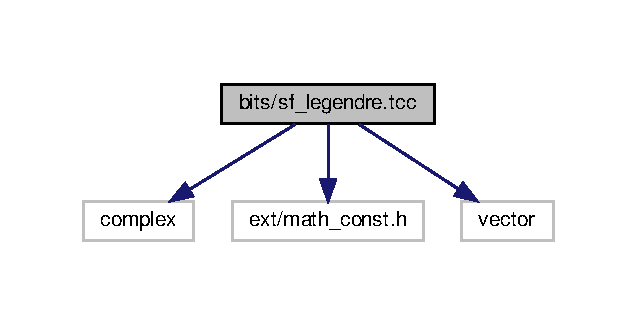
\includegraphics[width=172pt]{sf__legendre_8tcc__incl}
\end{center}
\end{figure}
\subsection*{Namespaces}
\begin{DoxyCompactItemize}
\item 
 \hyperlink{namespacestd}{std}
\item 
 \hyperlink{namespacestd_1_1____detail}{std\+::\+\_\+\+\_\+detail}
\end{DoxyCompactItemize}
\subsection*{Macros}
\begin{DoxyCompactItemize}
\item 
\#define \hyperlink{sf__legendre_8tcc_adf9a610f8b35f611eab3b1894e967c9f}{\+\_\+\+G\+L\+I\+B\+C\+X\+X\+\_\+\+B\+I\+T\+S\+\_\+\+S\+F\+\_\+\+L\+E\+G\+E\+N\+D\+R\+E\+\_\+\+T\+C\+C}~1
\end{DoxyCompactItemize}
\subsection*{Functions}
\begin{DoxyCompactItemize}
\item 
{\footnotesize template$<$typename \+\_\+\+Tp $>$ }\\\+\_\+\+Tp \hyperlink{namespacestd_1_1____detail_a8b31886e334427566b1b00d71052191b}{std\+::\+\_\+\+\_\+detail\+::\+\_\+\+\_\+assoc\+\_\+legendre\+\_\+p} (unsigned int \+\_\+\+\_\+l, unsigned int \+\_\+\+\_\+m, \+\_\+\+Tp \+\_\+\+\_\+x)
\begin{DoxyCompactList}\small\item\em Return the associated Legendre function by recursion on $ l $ and downward recursion on m. \end{DoxyCompactList}\item 
{\footnotesize template$<$typename \+\_\+\+Tp $>$ }\\\+\_\+\+Tp \hyperlink{namespacestd_1_1____detail_ad340d3fb1a429356292e7dcf61348c8a}{std\+::\+\_\+\+\_\+detail\+::\+\_\+\+\_\+poly\+\_\+legendre\+\_\+p} (unsigned int \+\_\+\+\_\+l, \+\_\+\+Tp \+\_\+\+\_\+x)
\begin{DoxyCompactList}\small\item\em Return the Legendre polynomial by upward recursion on order $ l $. \end{DoxyCompactList}\item 
{\footnotesize template$<$typename \+\_\+\+Tp $>$ }\\\+\_\+\+Tp \hyperlink{namespacestd_1_1____detail_aa810a501ad591480559e9f10d1b18e0f}{std\+::\+\_\+\+\_\+detail\+::\+\_\+\+\_\+poly\+\_\+legendre\+\_\+q} (unsigned int \+\_\+\+\_\+l, \+\_\+\+Tp \+\_\+\+\_\+x)
\begin{DoxyCompactList}\small\item\em Return the Legendre function of the second kind by upward recursion on order $ l $. \end{DoxyCompactList}\item 
{\footnotesize template$<$typename \+\_\+\+Tp $>$ }\\std\+::complex$<$ \+\_\+\+Tp $>$ \hyperlink{namespacestd_1_1____detail_a31b9beb882431d61d439862de0366eec}{std\+::\+\_\+\+\_\+detail\+::\+\_\+\+\_\+sph\+\_\+harmonic} (unsigned int \+\_\+\+\_\+l, int \+\_\+\+\_\+m, \+\_\+\+Tp \+\_\+\+\_\+theta, \+\_\+\+Tp \+\_\+\+\_\+phi)
\begin{DoxyCompactList}\small\item\em Return the spherical harmonic function. \end{DoxyCompactList}\item 
{\footnotesize template$<$typename \+\_\+\+Tp $>$ }\\\+\_\+\+Tp \hyperlink{namespacestd_1_1____detail_a1c819d02915bdc2ab5c7693513ce0be0}{std\+::\+\_\+\+\_\+detail\+::\+\_\+\+\_\+sph\+\_\+legendre} (unsigned int \+\_\+\+\_\+l, unsigned int \+\_\+\+\_\+m, \+\_\+\+Tp \+\_\+\+\_\+theta)
\begin{DoxyCompactList}\small\item\em Return the spherical associated Legendre function. \end{DoxyCompactList}\end{DoxyCompactItemize}


\subsection{Macro Definition Documentation}
\hypertarget{sf__legendre_8tcc_adf9a610f8b35f611eab3b1894e967c9f}{}\index{sf\+\_\+legendre.\+tcc@{sf\+\_\+legendre.\+tcc}!\+\_\+\+G\+L\+I\+B\+C\+X\+X\+\_\+\+B\+I\+T\+S\+\_\+\+S\+F\+\_\+\+L\+E\+G\+E\+N\+D\+R\+E\+\_\+\+T\+C\+C@{\+\_\+\+G\+L\+I\+B\+C\+X\+X\+\_\+\+B\+I\+T\+S\+\_\+\+S\+F\+\_\+\+L\+E\+G\+E\+N\+D\+R\+E\+\_\+\+T\+C\+C}}
\index{\+\_\+\+G\+L\+I\+B\+C\+X\+X\+\_\+\+B\+I\+T\+S\+\_\+\+S\+F\+\_\+\+L\+E\+G\+E\+N\+D\+R\+E\+\_\+\+T\+C\+C@{\+\_\+\+G\+L\+I\+B\+C\+X\+X\+\_\+\+B\+I\+T\+S\+\_\+\+S\+F\+\_\+\+L\+E\+G\+E\+N\+D\+R\+E\+\_\+\+T\+C\+C}!sf\+\_\+legendre.\+tcc@{sf\+\_\+legendre.\+tcc}}
\subsubsection[{\+\_\+\+G\+L\+I\+B\+C\+X\+X\+\_\+\+B\+I\+T\+S\+\_\+\+S\+F\+\_\+\+L\+E\+G\+E\+N\+D\+R\+E\+\_\+\+T\+C\+C}]{\setlength{\rightskip}{0pt plus 5cm}\#define \+\_\+\+G\+L\+I\+B\+C\+X\+X\+\_\+\+B\+I\+T\+S\+\_\+\+S\+F\+\_\+\+L\+E\+G\+E\+N\+D\+R\+E\+\_\+\+T\+C\+C~1}\label{sf__legendre_8tcc_adf9a610f8b35f611eab3b1894e967c9f}


Definition at line 47 of file sf\+\_\+legendre.\+tcc.


\hypertarget{sf__mod__bessel_8tcc}{}\section{bits/sf\+\_\+mod\+\_\+bessel.tcc File Reference}
\label{sf__mod__bessel_8tcc}\index{bits/sf\+\_\+mod\+\_\+bessel.\+tcc@{bits/sf\+\_\+mod\+\_\+bessel.\+tcc}}
{\ttfamily \#include $<$complex$>$}\\*
{\ttfamily \#include $<$utility$>$}\\*
{\ttfamily \#include $<$ext/math\+\_\+const.\+h$>$}\\*
Include dependency graph for sf\+\_\+mod\+\_\+bessel.\+tcc\+:
\nopagebreak
\begin{figure}[H]
\begin{center}
\leavevmode
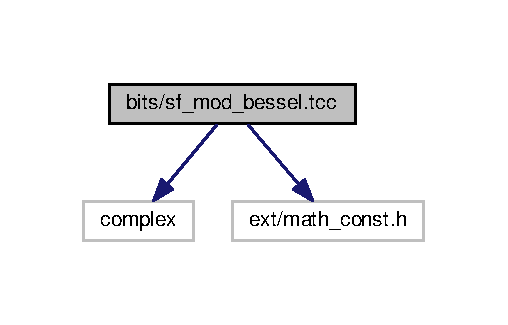
\includegraphics[width=302pt]{sf__mod__bessel_8tcc__incl}
\end{center}
\end{figure}
This graph shows which files directly or indirectly include this file\+:
\nopagebreak
\begin{figure}[H]
\begin{center}
\leavevmode
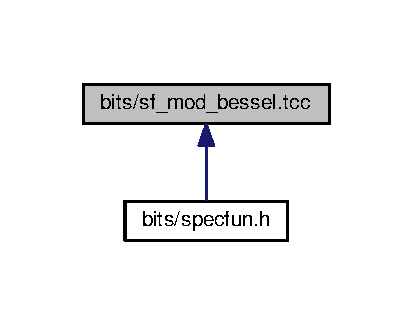
\includegraphics[width=198pt]{sf__mod__bessel_8tcc__dep__incl}
\end{center}
\end{figure}
\subsection*{Namespaces}
\begin{DoxyCompactItemize}
\item 
 \hyperlink{namespacestd}{std}
\item 
 \hyperlink{namespacestd_1_1____detail}{std\+::\+\_\+\+\_\+detail}
\end{DoxyCompactItemize}
\subsection*{Macros}
\begin{DoxyCompactItemize}
\item 
\#define \hyperlink{sf__mod__bessel_8tcc_a746f247a80ce9ef275dfb1cffbabeabd}{\+\_\+\+G\+L\+I\+B\+C\+X\+X\+\_\+\+B\+I\+T\+S\+\_\+\+S\+F\+\_\+\+M\+O\+D\+\_\+\+B\+E\+S\+S\+E\+L\+\_\+\+T\+CC}~1
\end{DoxyCompactItemize}
\subsection*{Functions}
\begin{DoxyCompactItemize}
\item 
{\footnotesize template$<$typename \+\_\+\+Tp $>$ }\\void \hyperlink{namespacestd_1_1____detail_aaf4b5556c6d01bad1892cb1515b22c64}{std\+::\+\_\+\+\_\+detail\+::\+\_\+\+\_\+airy} (\+\_\+\+Tp \+\_\+\+\_\+z, \+\_\+\+Tp \&\+\_\+\+Ai, \+\_\+\+Tp \&\+\_\+\+Bi, \+\_\+\+Tp \&\+\_\+\+Aip, \+\_\+\+Tp \&\+\_\+\+Bip)
\begin{DoxyCompactList}\small\item\em Compute the Airy functions $ Ai(x) $ and $ Bi(x) $ and their first derivatives $ Ai'(x) $ and $ Bi(x) $ respectively. \end{DoxyCompactList}\item 
{\footnotesize template$<$typename \+\_\+\+Tp $>$ }\\\+\_\+\+Tp \hyperlink{namespacestd_1_1____detail_a72e3392d5c03c0bc8f2b5ffb8c1304b5}{std\+::\+\_\+\+\_\+detail\+::\+\_\+\+\_\+cyl\+\_\+bessel\+\_\+i} (\+\_\+\+Tp \+\_\+\+\_\+nu, \+\_\+\+Tp \+\_\+\+\_\+x)
\begin{DoxyCompactList}\small\item\em Return the regular modified Bessel function of order $ \nu $\+: $ I_{\nu}(x) $. \end{DoxyCompactList}\item 
{\footnotesize template$<$typename \+\_\+\+Tp $>$ }\\void \hyperlink{namespacestd_1_1____detail_af699e7a6d31556df09f0a0db4f196cc0}{std\+::\+\_\+\+\_\+detail\+::\+\_\+\+\_\+cyl\+\_\+bessel\+\_\+ik} (\+\_\+\+Tp \+\_\+\+\_\+nu, \+\_\+\+Tp \+\_\+\+\_\+x, \+\_\+\+Tp \&\+\_\+\+Inu, \+\_\+\+Tp \&\+\_\+\+Knu, \+\_\+\+Tp \&\+\_\+\+Ipnu, \+\_\+\+Tp \&\+\_\+\+Kpnu)
\begin{DoxyCompactList}\small\item\em Return the modified cylindrical Bessel functions and their derivatives of order $ \nu $ by various means. \end{DoxyCompactList}\item 
{\footnotesize template$<$typename \+\_\+\+Tp $>$ }\\void \hyperlink{namespacestd_1_1____detail_a7386732bb6f0d45bbcbccaad436797a0}{std\+::\+\_\+\+\_\+detail\+::\+\_\+\+\_\+cyl\+\_\+bessel\+\_\+ik\+\_\+asymp} (\+\_\+\+Tp \+\_\+\+\_\+nu, \+\_\+\+Tp \+\_\+\+\_\+x, \+\_\+\+Tp \&\+\_\+\+Inu, \+\_\+\+Tp \&\+\_\+\+Knu, \+\_\+\+Tp \&\+\_\+\+Ipnu, \+\_\+\+Tp \&\+\_\+\+Kpnu)
\begin{DoxyCompactList}\small\item\em This routine computes the asymptotic modified cylindrical Bessel and functions of order nu\+: $ I_{\nu}(x) $, $ N_{\nu}(x) $. Use this for $ x >> nu^2 + 1 $. \end{DoxyCompactList}\item 
{\footnotesize template$<$typename \+\_\+\+Tp $>$ }\\void \hyperlink{namespacestd_1_1____detail_aed8927c2ec079a1831da66abcfae802b}{std\+::\+\_\+\+\_\+detail\+::\+\_\+\+\_\+cyl\+\_\+bessel\+\_\+ik\+\_\+steed} (\+\_\+\+Tp \+\_\+\+\_\+nu, \+\_\+\+Tp \+\_\+\+\_\+x, \+\_\+\+Tp \&\+\_\+\+Inu, \+\_\+\+Tp \&\+\_\+\+Knu, \+\_\+\+Tp \&\+\_\+\+Ipnu, \+\_\+\+Tp \&\+\_\+\+Kpnu)
\begin{DoxyCompactList}\small\item\em Compute the modified Bessel functions $ I_\nu(x) $ and $ K_\nu(x) $ and their first derivatives $ I'_\nu(x) $ and $ K'_\nu(x) $ respectively. These four functions are computed together for numerical stability. \end{DoxyCompactList}\item 
{\footnotesize template$<$typename \+\_\+\+Tp $>$ }\\\+\_\+\+Tp \hyperlink{namespacestd_1_1____detail_ac9152f2369a18aa795fe24ccfa6dcf12}{std\+::\+\_\+\+\_\+detail\+::\+\_\+\+\_\+cyl\+\_\+bessel\+\_\+k} (\+\_\+\+Tp \+\_\+\+\_\+nu, \+\_\+\+Tp \+\_\+\+\_\+x)
\begin{DoxyCompactList}\small\item\em Return the irregular modified Bessel function $ K_{\nu}(x) $ of order $ \nu $. \end{DoxyCompactList}\item 
{\footnotesize template$<$typename \+\_\+\+Tp $>$ }\\void \hyperlink{namespacestd_1_1____detail_a96ccd15b0c375170be157136faa47387}{std\+::\+\_\+\+\_\+detail\+::\+\_\+\+\_\+fock\+\_\+airy} (\+\_\+\+Tp \+\_\+\+\_\+x, std\+::complex$<$ \+\_\+\+Tp $>$ \&\+\_\+\+\_\+w1, std\+::complex$<$ \+\_\+\+Tp $>$ \&\+\_\+\+\_\+w2, std\+::complex$<$ \+\_\+\+Tp $>$ \&\+\_\+\+\_\+w1p, std\+::complex$<$ \+\_\+\+Tp $>$ \&\+\_\+\+\_\+w2p)
\begin{DoxyCompactList}\small\item\em Compute the Fock-\/type Airy functions $ w_1(x) $ and $ w_2(x) $ and their first derivatives $ w_1'(x) $ and $ w_2'(x) $ respectively. \[ w_1(x) = \sqrt{\pi}(Ai(x) + iBi(x)) \] \[ w_2(x) = \sqrt{\pi}(Ai(x) - iBi(x)) \]. \end{DoxyCompactList}\item 
{\footnotesize template$<$typename \+\_\+\+Tp $>$ }\\void \hyperlink{namespacestd_1_1____detail_a35edea916ec9c8310f7d4a06618f7378}{std\+::\+\_\+\+\_\+detail\+::\+\_\+\+\_\+sph\+\_\+bessel\+\_\+ik} (unsigned int \+\_\+\+\_\+n, \+\_\+\+Tp \+\_\+\+\_\+x, \+\_\+\+Tp \&\+\_\+\+\_\+i\+\_\+n, \+\_\+\+Tp \&\+\_\+\+\_\+k\+\_\+n, \+\_\+\+Tp \&\+\_\+\+\_\+ip\+\_\+n, \+\_\+\+Tp \&\+\_\+\+\_\+kp\+\_\+n)
\begin{DoxyCompactList}\small\item\em Compute the spherical modified Bessel functions $ i_n(x) $ and $ k_n(x) $ and their first derivatives $ i'_n(x) $ and $ k'_n(x) $ respectively. \end{DoxyCompactList}\end{DoxyCompactItemize}


\subsection{Detailed Description}
This is an internal header file, included by other library headers. Do not attempt to use it directly. Instead, include $<$cmath$>$. 

\subsection{Macro Definition Documentation}
\index{sf\+\_\+mod\+\_\+bessel.\+tcc@{sf\+\_\+mod\+\_\+bessel.\+tcc}!\+\_\+\+G\+L\+I\+B\+C\+X\+X\+\_\+\+B\+I\+T\+S\+\_\+\+S\+F\+\_\+\+M\+O\+D\+\_\+\+B\+E\+S\+S\+E\+L\+\_\+\+T\+CC@{\+\_\+\+G\+L\+I\+B\+C\+X\+X\+\_\+\+B\+I\+T\+S\+\_\+\+S\+F\+\_\+\+M\+O\+D\+\_\+\+B\+E\+S\+S\+E\+L\+\_\+\+T\+CC}}
\index{\+\_\+\+G\+L\+I\+B\+C\+X\+X\+\_\+\+B\+I\+T\+S\+\_\+\+S\+F\+\_\+\+M\+O\+D\+\_\+\+B\+E\+S\+S\+E\+L\+\_\+\+T\+CC@{\+\_\+\+G\+L\+I\+B\+C\+X\+X\+\_\+\+B\+I\+T\+S\+\_\+\+S\+F\+\_\+\+M\+O\+D\+\_\+\+B\+E\+S\+S\+E\+L\+\_\+\+T\+CC}!sf\+\_\+mod\+\_\+bessel.\+tcc@{sf\+\_\+mod\+\_\+bessel.\+tcc}}
\subsubsection[{\texorpdfstring{\+\_\+\+G\+L\+I\+B\+C\+X\+X\+\_\+\+B\+I\+T\+S\+\_\+\+S\+F\+\_\+\+M\+O\+D\+\_\+\+B\+E\+S\+S\+E\+L\+\_\+\+T\+CC}{_GLIBCXX_BITS_SF_MOD_BESSEL_TCC}}]{\setlength{\rightskip}{0pt plus 5cm}\#define \+\_\+\+G\+L\+I\+B\+C\+X\+X\+\_\+\+B\+I\+T\+S\+\_\+\+S\+F\+\_\+\+M\+O\+D\+\_\+\+B\+E\+S\+S\+E\+L\+\_\+\+T\+CC~1}\hypertarget{sf__mod__bessel_8tcc_a746f247a80ce9ef275dfb1cffbabeabd}{}\label{sf__mod__bessel_8tcc_a746f247a80ce9ef275dfb1cffbabeabd}


Definition at line 47 of file sf\+\_\+mod\+\_\+bessel.\+tcc.


\hypertarget{sf__owens__t_8tcc}{}\section{bits/sf\+\_\+owens\+\_\+t.tcc File Reference}
\label{sf__owens__t_8tcc}\index{bits/sf\+\_\+owens\+\_\+t.\+tcc@{bits/sf\+\_\+owens\+\_\+t.\+tcc}}
This graph shows which files directly or indirectly include this file\+:
\nopagebreak
\begin{figure}[H]
\begin{center}
\leavevmode
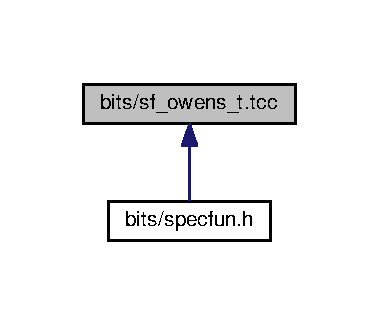
\includegraphics[width=182pt]{sf__owens__t_8tcc__dep__incl}
\end{center}
\end{figure}
\subsection*{Namespaces}
\begin{DoxyCompactItemize}
\item 
 \hyperlink{namespacestd}{std}
\item 
 \hyperlink{namespacestd_1_1____detail}{std\+::\+\_\+\+\_\+detail}
\end{DoxyCompactItemize}
\subsection*{Macros}
\begin{DoxyCompactItemize}
\item 
\#define \hyperlink{sf__owens__t_8tcc_a5986cbb2c459a5e859ffe2fe1fa7cd25}{\+\_\+\+G\+L\+I\+B\+C\+X\+X\+\_\+\+B\+I\+T\+S\+\_\+\+S\+F\+\_\+\+O\+W\+E\+N\+S\+\_\+\+T\+\_\+\+T\+CC}~1
\end{DoxyCompactItemize}
\subsection*{Functions}
\begin{DoxyCompactItemize}
\item 
{\footnotesize template$<$typename \+\_\+\+Tp $>$ }\\\+\_\+\+Tp \hyperlink{namespacestd_1_1____detail_afdb25beb2328b74d64d9be03de64c442}{std\+::\+\_\+\+\_\+detail\+::\+\_\+\+\_\+gauss} (\+\_\+\+Tp \+\_\+\+\_\+x)
\item 
{\footnotesize template$<$typename \+\_\+\+Tp $>$ }\\\+\_\+\+Tp \hyperlink{namespacestd_1_1____detail_a5b50a9d8beaca5a637c8293ab01bf124}{std\+::\+\_\+\+\_\+detail\+::\+\_\+\+\_\+owens\+\_\+t} (\+\_\+\+Tp \+\_\+\+\_\+h, \+\_\+\+Tp \+\_\+\+\_\+a)
\item 
{\footnotesize template$<$typename \+\_\+\+Tp $>$ }\\\+\_\+\+Tp \hyperlink{namespacestd_1_1____detail_a6827b123253cc6a19947406339738bd7}{std\+::\+\_\+\+\_\+detail\+::\+\_\+\+\_\+znorm1} (\+\_\+\+Tp \+\_\+\+\_\+x)
\item 
{\footnotesize template$<$typename \+\_\+\+Tp $>$ }\\\+\_\+\+Tp \hyperlink{namespacestd_1_1____detail_adf930b70ca943c6810ac7d2ea78d2cc3}{std\+::\+\_\+\+\_\+detail\+::\+\_\+\+\_\+znorm2} (\+\_\+\+Tp \+\_\+\+\_\+x)
\end{DoxyCompactItemize}


\subsection{Detailed Description}
This is an internal header file, included by other library headers. You should not attempt to use it directly. 

\subsection{Macro Definition Documentation}
\index{sf\+\_\+owens\+\_\+t.\+tcc@{sf\+\_\+owens\+\_\+t.\+tcc}!\+\_\+\+G\+L\+I\+B\+C\+X\+X\+\_\+\+B\+I\+T\+S\+\_\+\+S\+F\+\_\+\+O\+W\+E\+N\+S\+\_\+\+T\+\_\+\+T\+CC@{\+\_\+\+G\+L\+I\+B\+C\+X\+X\+\_\+\+B\+I\+T\+S\+\_\+\+S\+F\+\_\+\+O\+W\+E\+N\+S\+\_\+\+T\+\_\+\+T\+CC}}
\index{\+\_\+\+G\+L\+I\+B\+C\+X\+X\+\_\+\+B\+I\+T\+S\+\_\+\+S\+F\+\_\+\+O\+W\+E\+N\+S\+\_\+\+T\+\_\+\+T\+CC@{\+\_\+\+G\+L\+I\+B\+C\+X\+X\+\_\+\+B\+I\+T\+S\+\_\+\+S\+F\+\_\+\+O\+W\+E\+N\+S\+\_\+\+T\+\_\+\+T\+CC}!sf\+\_\+owens\+\_\+t.\+tcc@{sf\+\_\+owens\+\_\+t.\+tcc}}
\subsubsection[{\texorpdfstring{\+\_\+\+G\+L\+I\+B\+C\+X\+X\+\_\+\+B\+I\+T\+S\+\_\+\+S\+F\+\_\+\+O\+W\+E\+N\+S\+\_\+\+T\+\_\+\+T\+CC}{_GLIBCXX_BITS_SF_OWENS_T_TCC}}]{\setlength{\rightskip}{0pt plus 5cm}\#define \+\_\+\+G\+L\+I\+B\+C\+X\+X\+\_\+\+B\+I\+T\+S\+\_\+\+S\+F\+\_\+\+O\+W\+E\+N\+S\+\_\+\+T\+\_\+\+T\+CC~1}\hypertarget{sf__owens__t_8tcc_a5986cbb2c459a5e859ffe2fe1fa7cd25}{}\label{sf__owens__t_8tcc_a5986cbb2c459a5e859ffe2fe1fa7cd25}


Definition at line 31 of file sf\+\_\+owens\+\_\+t.\+tcc.


\hypertarget{sf__polylog_8tcc}{}\section{bits/sf\+\_\+polylog.tcc File Reference}
\label{sf__polylog_8tcc}\index{bits/sf\+\_\+polylog.\+tcc@{bits/sf\+\_\+polylog.\+tcc}}
{\ttfamily \#include $<$ext/math\+\_\+const.\+h$>$}\\*
Include dependency graph for sf\+\_\+polylog.\+tcc\+:
\nopagebreak
\begin{figure}[H]
\begin{center}
\leavevmode
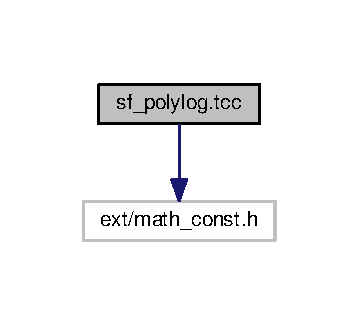
\includegraphics[width=176pt]{sf__polylog_8tcc__incl}
\end{center}
\end{figure}
This graph shows which files directly or indirectly include this file\+:
\nopagebreak
\begin{figure}[H]
\begin{center}
\leavevmode
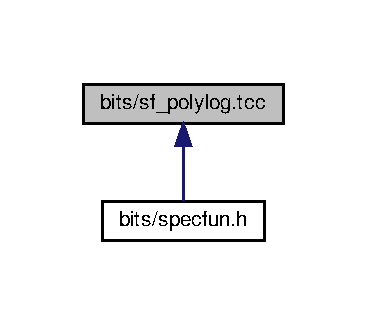
\includegraphics[width=176pt]{sf__polylog_8tcc__dep__incl}
\end{center}
\end{figure}
\subsection*{Namespaces}
\begin{DoxyCompactItemize}
\item 
 \hyperlink{namespacestd}{std}
\item 
 \hyperlink{namespacestd_1_1____detail}{std\+::\+\_\+\+\_\+detail}
\end{DoxyCompactItemize}
\subsection*{Macros}
\begin{DoxyCompactItemize}
\item 
\#define \hyperlink{sf__polylog_8tcc_ab6c10ff949c404f48f72645a3fe8a674}{\+\_\+\+G\+L\+I\+B\+C\+X\+X\+\_\+\+B\+I\+T\+S\+\_\+\+S\+F\+\_\+\+P\+O\+L\+Y\+L\+O\+G\+\_\+\+T\+C\+C}~1
\end{DoxyCompactItemize}
\subsection*{Functions}
\begin{DoxyCompactItemize}
\item 
{\footnotesize template$<$typename \+\_\+\+Tp $>$ }\\\+\_\+\+Tp \hyperlink{namespacestd_1_1____detail_a4c199ebf92e53a3ae9c27c2c79d65e21}{std\+::\+\_\+\+\_\+detail\+::\+\_\+\+\_\+bose\+\_\+einstein} (\+\_\+\+Tp \+\_\+\+\_\+s, \+\_\+\+Tp \+\_\+\+\_\+x)
\item 
{\footnotesize template$<$typename \+\_\+\+Tp $>$ }\\std\+::complex$<$ \+\_\+\+Tp $>$ \hyperlink{namespacestd_1_1____detail_a49702394cf9b45acfa5b84f232078a9b}{std\+::\+\_\+\+\_\+detail\+::\+\_\+\+\_\+clamp\+\_\+0\+\_\+m2pi} (std\+::complex$<$ \+\_\+\+Tp $>$ \+\_\+\+\_\+w)
\item 
{\footnotesize template$<$typename \+\_\+\+Tp $>$ }\\std\+::complex$<$ \+\_\+\+Tp $>$ \hyperlink{namespacestd_1_1____detail_afc1fa8ae4623bdc71b3bf21671f68e38}{std\+::\+\_\+\+\_\+detail\+::\+\_\+\+\_\+clamp\+\_\+pi} (std\+::complex$<$ \+\_\+\+Tp $>$ \+\_\+\+\_\+w)
\item 
{\footnotesize template$<$typename \+\_\+\+Tp $>$ }\\std\+::complex$<$ \+\_\+\+Tp $>$ \hyperlink{namespacestd_1_1____detail_a260f2c50d0164a55dab6a95217ced893}{std\+::\+\_\+\+\_\+detail\+::\+\_\+\+\_\+clausen} (unsigned int \+\_\+\+\_\+m, std\+::complex$<$ \+\_\+\+Tp $>$ \+\_\+\+\_\+w)
\item 
{\footnotesize template$<$typename \+\_\+\+Tp $>$ }\\\+\_\+\+Tp \hyperlink{namespacestd_1_1____detail_a12dab8bfc7bc5554fe0db5d1777d9887}{std\+::\+\_\+\+\_\+detail\+::\+\_\+\+\_\+clausen} (unsigned int \+\_\+\+\_\+m, \+\_\+\+Tp \+\_\+\+\_\+w)
\item 
{\footnotesize template$<$typename \+\_\+\+Tp $>$ }\\\+\_\+\+Tp \hyperlink{namespacestd_1_1____detail_a06b95eeefe47e8899e2e0a6bbd3ad31b}{std\+::\+\_\+\+\_\+detail\+::\+\_\+\+\_\+clausen\+\_\+c} (unsigned int \+\_\+\+\_\+m, std\+::complex$<$ \+\_\+\+Tp $>$ \+\_\+\+\_\+w)
\item 
{\footnotesize template$<$typename \+\_\+\+Tp $>$ }\\\+\_\+\+Tp \hyperlink{namespacestd_1_1____detail_a44f2a2f49402b847c8408da5b18f8107}{std\+::\+\_\+\+\_\+detail\+::\+\_\+\+\_\+clausen\+\_\+c} (unsigned int \+\_\+\+\_\+m, \+\_\+\+Tp \+\_\+\+\_\+w)
\item 
{\footnotesize template$<$typename \+\_\+\+Tp $>$ }\\\+\_\+\+Tp \hyperlink{namespacestd_1_1____detail_a19bb52bc473e5c3811281acbbdefa869}{std\+::\+\_\+\+\_\+detail\+::\+\_\+\+\_\+clausen\+\_\+s} (unsigned int \+\_\+\+\_\+m, std\+::complex$<$ \+\_\+\+Tp $>$ \+\_\+\+\_\+w)
\item 
{\footnotesize template$<$typename \+\_\+\+Tp $>$ }\\\+\_\+\+Tp \hyperlink{namespacestd_1_1____detail_a1b8a79cb99cbbe5ebbbc16a1dfa7d2c1}{std\+::\+\_\+\+\_\+detail\+::\+\_\+\+\_\+clausen\+\_\+s} (unsigned int \+\_\+\+\_\+m, \+\_\+\+Tp \+\_\+\+\_\+w)
\item 
{\footnotesize template$<$typename \+\_\+\+Tp $>$ }\\\+\_\+\+Tp \hyperlink{namespacestd_1_1____detail_ae2e1407cd73ed7ca37c9085971d64787}{std\+::\+\_\+\+\_\+detail\+::\+\_\+\+\_\+dirichlet\+\_\+beta} (std\+::complex$<$ \+\_\+\+Tp $>$ \+\_\+\+\_\+w)
\item 
{\footnotesize template$<$typename \+\_\+\+Tp $>$ }\\\+\_\+\+Tp \hyperlink{namespacestd_1_1____detail_a6cedea78253fd4d6da481c681a2eed72}{std\+::\+\_\+\+\_\+detail\+::\+\_\+\+\_\+dirichlet\+\_\+beta} (\+\_\+\+Tp \+\_\+\+\_\+w)
\item 
{\footnotesize template$<$typename \+\_\+\+Tp $>$ }\\std\+::complex$<$ \+\_\+\+Tp $>$ \hyperlink{namespacestd_1_1____detail_ac00ca43b3035da757d982b43d2c59bc1}{std\+::\+\_\+\+\_\+detail\+::\+\_\+\+\_\+dirichlet\+\_\+eta} (std\+::complex$<$ \+\_\+\+Tp $>$ \+\_\+\+\_\+w)
\item 
{\footnotesize template$<$typename \+\_\+\+Tp $>$ }\\\+\_\+\+Tp \hyperlink{namespacestd_1_1____detail_acd1e2a576d04658c6332df91cdaacd6e}{std\+::\+\_\+\+\_\+detail\+::\+\_\+\+\_\+dirichlet\+\_\+eta} (\+\_\+\+Tp \+\_\+\+\_\+w)
\item 
{\footnotesize template$<$typename \+\_\+\+Tp $>$ }\\\+\_\+\+Tp \hyperlink{namespacestd_1_1____detail_a6057422cd4e359f44dcdb6cffc26128f}{std\+::\+\_\+\+\_\+detail\+::\+\_\+\+\_\+fermi\+\_\+dirac} (\+\_\+\+Tp \+\_\+\+\_\+s, \+\_\+\+Tp \+\_\+\+\_\+x)
\item 
{\footnotesize template$<$typename \+\_\+\+Tp $>$ }\\bool \hyperlink{namespacestd_1_1____detail_acefbc7637e41168e49d6230df9c5127f}{std\+::\+\_\+\+\_\+detail\+::\+\_\+\+\_\+fpequal} (const \+\_\+\+Tp \&\+\_\+\+\_\+a, const \+\_\+\+Tp \&\+\_\+\+\_\+b)
\item 
{\footnotesize template$<$typename \+\_\+\+Tp $>$ }\\bool \hyperlink{namespacestd_1_1____detail_a990a8fb06307793ceae4c3c288f8b876}{std\+::\+\_\+\+\_\+detail\+::\+\_\+\+\_\+fpimag} (const std\+::complex$<$ \+\_\+\+Tp $>$ \&\+\_\+\+\_\+w)
\item 
{\footnotesize template$<$typename \+\_\+\+Tp $>$ }\\bool \hyperlink{namespacestd_1_1____detail_a962bc8055b3948b6e2bebf34f86d9263}{std\+::\+\_\+\+\_\+detail\+::\+\_\+\+\_\+fpimag} (const \+\_\+\+Tp)
\item 
{\footnotesize template$<$typename \+\_\+\+Tp $>$ }\\bool \hyperlink{namespacestd_1_1____detail_ab78bb436e256ef9a3f64fa2a1ce25fb1}{std\+::\+\_\+\+\_\+detail\+::\+\_\+\+\_\+fpreal} (const std\+::complex$<$ \+\_\+\+Tp $>$ \&\+\_\+\+\_\+w)
\item 
{\footnotesize template$<$typename \+\_\+\+Tp $>$ }\\bool \hyperlink{namespacestd_1_1____detail_a52087623539a401ded28ef1ca8fbcd04}{std\+::\+\_\+\+\_\+detail\+::\+\_\+\+\_\+fpreal} (const \+\_\+\+Tp)
\item 
{\footnotesize template$<$typename \+\_\+\+Tp $>$ }\\std\+::complex$<$ F\+P\+Type $>$ \hyperlink{namespacestd_1_1____detail_a8381d5cd047b45387ab2d0ef3591171c}{std\+::\+\_\+\+\_\+detail\+::\+\_\+\+\_\+hurwitz\+\_\+zeta} (const \+\_\+\+Tp \+\_\+\+\_\+s, std\+::complex$<$ \+\_\+\+Tp $>$ \+\_\+\+\_\+a)
\item 
{\footnotesize template$<$typename \+\_\+\+Tp $>$ }\\\+\_\+\+Tp \hyperlink{namespacestd_1_1____detail_a17fb8cea11706f319aaea277188a29c8}{std\+::\+\_\+\+\_\+detail\+::\+\_\+\+\_\+polylog} (\+\_\+\+Tp \+\_\+\+\_\+s, \+\_\+\+Tp \+\_\+\+\_\+x)
\item 
{\footnotesize template$<$typename \+\_\+\+Tp $>$ }\\std\+::complex$<$ \+\_\+\+Tp $>$ \hyperlink{namespacestd_1_1____detail_aa14e3ca6e4bee5ac1f1e5e1c2cee1d5a}{std\+::\+\_\+\+\_\+detail\+::\+\_\+\+\_\+polylog} (\+\_\+\+Tp \+\_\+\+\_\+s, std\+::complex$<$ \+\_\+\+Tp $>$ \+\_\+\+\_\+w)
\item 
{\footnotesize template$<$typename \+\_\+\+Tp , typename Arg\+Type $>$ }\\\+\_\+\+\_\+gnu\+\_\+cxx\+::\+\_\+\+\_\+promote\+\_\+num\+\_\+t$<$ std\+::complex$<$ \+\_\+\+Tp $>$, Arg\+Type $>$ \hyperlink{namespacestd_1_1____detail_ad01c033a96c9f185216d6c9f9db49c99}{std\+::\+\_\+\+\_\+detail\+::\+\_\+\+\_\+polylog\+\_\+exp} (\+\_\+\+Tp \+\_\+\+\_\+s, Arg\+Type \+\_\+\+\_\+w)
\item 
{\footnotesize template$<$typename \+\_\+\+Tp $>$ }\\std\+::complex$<$ \+\_\+\+Tp $>$ \hyperlink{namespacestd_1_1____detail_a84b83a6be0a236fbcbbdea9078e8ca58}{std\+::\+\_\+\+\_\+detail\+::\+\_\+\+\_\+polylog\+\_\+exp\+\_\+asymp} (const \+\_\+\+Tp \+\_\+\+\_\+s, std\+::complex$<$ \+\_\+\+Tp $>$ \+\_\+\+\_\+w)
\item 
{\footnotesize template$<$typename \+\_\+\+Tp $>$ }\\std\+::complex$<$ \+\_\+\+Tp $>$ \hyperlink{namespacestd_1_1____detail_af7e0c042cba3c3ffc60844b1e0d545a6}{std\+::\+\_\+\+\_\+detail\+::\+\_\+\+\_\+polylog\+\_\+exp\+\_\+int\+\_\+neg} (const int \+\_\+\+\_\+s, std\+::complex$<$ \+\_\+\+Tp $>$ \+\_\+\+\_\+w)
\item 
{\footnotesize template$<$typename \+\_\+\+Tp $>$ }\\std\+::complex$<$ \+\_\+\+Tp $>$ \hyperlink{namespacestd_1_1____detail_a7d1d29f2a53007e83c70e9ef805d0ffa}{std\+::\+\_\+\+\_\+detail\+::\+\_\+\+\_\+polylog\+\_\+exp\+\_\+int\+\_\+neg} (const int \+\_\+\+\_\+s, \+\_\+\+Tp \+\_\+\+\_\+w)
\item 
{\footnotesize template$<$typename \+\_\+\+Tp $>$ }\\std\+::complex$<$ \+\_\+\+Tp $>$ \hyperlink{namespacestd_1_1____detail_a28317fd26d839f4e1cea72be3418508e}{std\+::\+\_\+\+\_\+detail\+::\+\_\+\+\_\+polylog\+\_\+exp\+\_\+int\+\_\+pos} (const unsigned int \+\_\+\+\_\+s, std\+::complex$<$ \+\_\+\+Tp $>$ \+\_\+\+\_\+w)
\item 
{\footnotesize template$<$typename \+\_\+\+Tp $>$ }\\std\+::complex$<$ \+\_\+\+Tp $>$ \hyperlink{namespacestd_1_1____detail_ac87302233a0ea200b1fb9a2592da21e6}{std\+::\+\_\+\+\_\+detail\+::\+\_\+\+\_\+polylog\+\_\+exp\+\_\+int\+\_\+pos} (const unsigned int \+\_\+\+\_\+s, \+\_\+\+Tp \+\_\+\+\_\+w)
\item 
{\footnotesize template$<$typename \+\_\+\+Tp $>$ }\\std\+::complex$<$ \+\_\+\+Tp $>$ \hyperlink{namespacestd_1_1____detail_a07b26b8c7ff467310e4e1df6e3efd893}{std\+::\+\_\+\+\_\+detail\+::\+\_\+\+\_\+polylog\+\_\+exp\+\_\+neg} (\+\_\+\+Tp \+\_\+\+\_\+s, std\+::complex$<$ \+\_\+\+Tp $>$ \+\_\+\+\_\+w)
\item 
{\footnotesize template$<$typename \+\_\+\+Tp $>$ }\\std\+::complex$<$ \+\_\+\+Tp $>$ \hyperlink{namespacestd_1_1____detail_aac54584aa89fef6a08a258ad6e2a75f5}{std\+::\+\_\+\+\_\+detail\+::\+\_\+\+\_\+polylog\+\_\+exp\+\_\+neg} (int \+\_\+\+\_\+s, std\+::complex$<$ \+\_\+\+Tp $>$ \+\_\+\+\_\+w)
\item 
{\footnotesize template$<$typename \+\_\+\+Tp , int \+\_\+\+\_\+sigma$>$ }\\std\+::complex$<$ \+\_\+\+Tp $>$ \hyperlink{namespacestd_1_1____detail_affdff8c867d264b62a64427e53f5b9aa}{std\+::\+\_\+\+\_\+detail\+::\+\_\+\+\_\+polylog\+\_\+exp\+\_\+neg\+\_\+even} (unsigned int \+\_\+\+\_\+n, std\+::complex$<$ \+\_\+\+Tp $>$ \+\_\+\+\_\+w)
\item 
{\footnotesize template$<$typename \+\_\+\+Tp , int \+\_\+\+\_\+sigma$>$ }\\std\+::complex$<$ \+\_\+\+Tp $>$ \hyperlink{namespacestd_1_1____detail_a114ec67e6802a402064b16a9a77f0863}{std\+::\+\_\+\+\_\+detail\+::\+\_\+\+\_\+polylog\+\_\+exp\+\_\+neg\+\_\+odd} (unsigned int \+\_\+\+\_\+n, std\+::complex$<$ \+\_\+\+Tp $>$ \+\_\+\+\_\+w)
\item 
{\footnotesize template$<$typename \+\_\+\+Pow\+Tp , typename \+\_\+\+Tp $>$ }\\\+\_\+\+Tp \hyperlink{namespacestd_1_1____detail_a466240361bcf30941d84a8fc3cd91cf9}{std\+::\+\_\+\+\_\+detail\+::\+\_\+\+\_\+polylog\+\_\+exp\+\_\+negative\+\_\+real\+\_\+part} (\+\_\+\+Pow\+Tp \+\_\+\+\_\+s, \+\_\+\+Tp \+\_\+\+\_\+w)
\item 
{\footnotesize template$<$typename \+\_\+\+Tp $>$ }\\std\+::complex$<$ \+\_\+\+Tp $>$ \hyperlink{namespacestd_1_1____detail_a0327d2970eba3a0a2d73c71c7a77701c}{std\+::\+\_\+\+\_\+detail\+::\+\_\+\+\_\+polylog\+\_\+exp\+\_\+pos} (unsigned int \+\_\+\+\_\+s, std\+::complex$<$ \+\_\+\+Tp $>$ \+\_\+\+\_\+w)
\item 
{\footnotesize template$<$typename \+\_\+\+Tp $>$ }\\std\+::complex$<$ \+\_\+\+Tp $>$ \hyperlink{namespacestd_1_1____detail_ab13a4be6685dd222b654da3297342d7e}{std\+::\+\_\+\+\_\+detail\+::\+\_\+\+\_\+polylog\+\_\+exp\+\_\+pos} (unsigned int \+\_\+\+\_\+s, \+\_\+\+Tp \+\_\+\+\_\+w)
\item 
{\footnotesize template$<$typename \+\_\+\+Tp $>$ }\\std\+::complex$<$ \+\_\+\+Tp $>$ \hyperlink{namespacestd_1_1____detail_a56b0f5bc6f4955469fd5f83105cbd466}{std\+::\+\_\+\+\_\+detail\+::\+\_\+\+\_\+polylog\+\_\+exp\+\_\+pos} (\+\_\+\+Tp \+\_\+\+\_\+s, std\+::complex$<$ \+\_\+\+Tp $>$ \+\_\+\+\_\+w)
\item 
{\footnotesize template$<$typename \+\_\+\+Tp $>$ }\\std\+::complex$<$ \+\_\+\+Tp $>$ \hyperlink{namespacestd_1_1____detail_abe2e38af779623f338c77dc46ac673bd}{std\+::\+\_\+\+\_\+detail\+::\+\_\+\+\_\+polylog\+\_\+exp\+\_\+real\+\_\+neg} (\+\_\+\+Tp \+\_\+\+\_\+s, std\+::complex$<$ \+\_\+\+Tp $>$ \+\_\+\+\_\+w)
\item 
{\footnotesize template$<$typename \+\_\+\+Tp $>$ }\\std\+::complex$<$ \+\_\+\+Tp $>$ \hyperlink{namespacestd_1_1____detail_ac9ae4e4771187bac37c1ccc83719feb2}{std\+::\+\_\+\+\_\+detail\+::\+\_\+\+\_\+polylog\+\_\+exp\+\_\+real\+\_\+neg} (\+\_\+\+Tp \+\_\+\+\_\+s, \+\_\+\+Tp \+\_\+\+\_\+w)
\item 
{\footnotesize template$<$typename \+\_\+\+Tp $>$ }\\std\+::complex$<$ \+\_\+\+Tp $>$ \hyperlink{namespacestd_1_1____detail_ab27023a3d94393d41c994000b2c16684}{std\+::\+\_\+\+\_\+detail\+::\+\_\+\+\_\+polylog\+\_\+exp\+\_\+real\+\_\+pos} (\+\_\+\+Tp \+\_\+\+\_\+s, std\+::complex$<$ \+\_\+\+Tp $>$ \+\_\+\+\_\+w)
\item 
{\footnotesize template$<$typename \+\_\+\+Tp $>$ }\\std\+::complex$<$ \+\_\+\+Tp $>$ \hyperlink{namespacestd_1_1____detail_ad77bb9953443dfb1575a61a4573c6913}{std\+::\+\_\+\+\_\+detail\+::\+\_\+\+\_\+polylog\+\_\+exp\+\_\+real\+\_\+pos} (\+\_\+\+Tp \+\_\+\+\_\+s, \+\_\+\+Tp \+\_\+\+\_\+w)
\item 
{\footnotesize template$<$typename \+\_\+\+Tp  = double$>$ }\\\+\_\+\+Tp \hyperlink{namespacestd_1_1____detail_af59bd2be508cc6a421ddf5dd70c93d97}{std\+::\+\_\+\+\_\+detail\+::evenzeta} (unsigned int \+\_\+\+\_\+k)
\end{DoxyCompactItemize}


\subsection{Detailed Description}
This is an internal header file, included by other library headers. Do not attempt to use it directly. Instead, include $<$cmath$>$. 

\subsection{Macro Definition Documentation}
\hypertarget{sf__polylog_8tcc_ab6c10ff949c404f48f72645a3fe8a674}{}\index{sf\+\_\+polylog.\+tcc@{sf\+\_\+polylog.\+tcc}!\+\_\+\+G\+L\+I\+B\+C\+X\+X\+\_\+\+B\+I\+T\+S\+\_\+\+S\+F\+\_\+\+P\+O\+L\+Y\+L\+O\+G\+\_\+\+T\+C\+C@{\+\_\+\+G\+L\+I\+B\+C\+X\+X\+\_\+\+B\+I\+T\+S\+\_\+\+S\+F\+\_\+\+P\+O\+L\+Y\+L\+O\+G\+\_\+\+T\+C\+C}}
\index{\+\_\+\+G\+L\+I\+B\+C\+X\+X\+\_\+\+B\+I\+T\+S\+\_\+\+S\+F\+\_\+\+P\+O\+L\+Y\+L\+O\+G\+\_\+\+T\+C\+C@{\+\_\+\+G\+L\+I\+B\+C\+X\+X\+\_\+\+B\+I\+T\+S\+\_\+\+S\+F\+\_\+\+P\+O\+L\+Y\+L\+O\+G\+\_\+\+T\+C\+C}!sf\+\_\+polylog.\+tcc@{sf\+\_\+polylog.\+tcc}}
\subsubsection[{\+\_\+\+G\+L\+I\+B\+C\+X\+X\+\_\+\+B\+I\+T\+S\+\_\+\+S\+F\+\_\+\+P\+O\+L\+Y\+L\+O\+G\+\_\+\+T\+C\+C}]{\setlength{\rightskip}{0pt plus 5cm}\#define \+\_\+\+G\+L\+I\+B\+C\+X\+X\+\_\+\+B\+I\+T\+S\+\_\+\+S\+F\+\_\+\+P\+O\+L\+Y\+L\+O\+G\+\_\+\+T\+C\+C~1}\label{sf__polylog_8tcc_ab6c10ff949c404f48f72645a3fe8a674}


Definition at line 41 of file sf\+\_\+polylog.\+tcc.


\hypertarget{sf__theta_8tcc}{}\section{include/bits/sf\+\_\+theta.tcc File Reference}
\label{sf__theta_8tcc}\index{include/bits/sf\+\_\+theta.\+tcc@{include/bits/sf\+\_\+theta.\+tcc}}
{\ttfamily \#include $<$vector$>$}\newline
{\ttfamily \#include $<$tuple$>$}\newline
{\ttfamily \#include $<$ext/math\+\_\+const.\+h$>$}\newline
Include dependency graph for sf\+\_\+theta.\+tcc\+:
\nopagebreak
\begin{figure}[H]
\begin{center}
\leavevmode
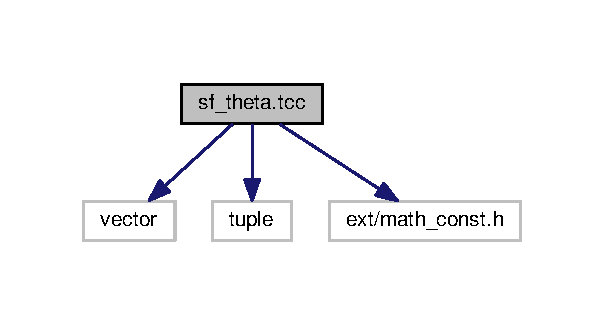
\includegraphics[width=290pt]{sf__theta_8tcc__incl}
\end{center}
\end{figure}
This graph shows which files directly or indirectly include this file\+:
\nopagebreak
\begin{figure}[H]
\begin{center}
\leavevmode
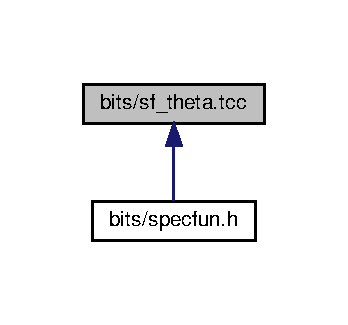
\includegraphics[width=201pt]{sf__theta_8tcc__dep__incl}
\end{center}
\end{figure}
\subsection*{Classes}
\begin{DoxyCompactItemize}
\item 
struct \hyperlink{structstd_1_1____detail_1_1____jacobi__lattice__t}{std\+::\+\_\+\+\_\+detail\+::\+\_\+\+\_\+jacobi\+\_\+lattice\+\_\+t$<$ \+\_\+\+Tp\+\_\+\+Omega1, \+\_\+\+Tp\+\_\+\+Omega3 $>$}
\item 
struct \hyperlink{structstd_1_1____detail_1_1____jacobi__lattice__t_1_1____arg__t}{std\+::\+\_\+\+\_\+detail\+::\+\_\+\+\_\+jacobi\+\_\+lattice\+\_\+t$<$ \+\_\+\+Tp\+\_\+\+Omega1, \+\_\+\+Tp\+\_\+\+Omega3 $>$\+::\+\_\+\+\_\+arg\+\_\+t}
\item 
struct \hyperlink{structstd_1_1____detail_1_1____jacobi__lattice__t_1_1____tau__t}{std\+::\+\_\+\+\_\+detail\+::\+\_\+\+\_\+jacobi\+\_\+lattice\+\_\+t$<$ \+\_\+\+Tp\+\_\+\+Omega1, \+\_\+\+Tp\+\_\+\+Omega3 $>$\+::\+\_\+\+\_\+tau\+\_\+t}
\item 
struct \hyperlink{structstd_1_1____detail_1_1____jacobi__theta__0__t}{std\+::\+\_\+\+\_\+detail\+::\+\_\+\+\_\+jacobi\+\_\+theta\+\_\+0\+\_\+t$<$ \+\_\+\+Tp1, \+\_\+\+Tp3 $>$}
\item 
struct \hyperlink{structstd_1_1____detail_1_1____weierstrass__invariants__t}{std\+::\+\_\+\+\_\+detail\+::\+\_\+\+\_\+weierstrass\+\_\+invariants\+\_\+t$<$ \+\_\+\+Tp1, \+\_\+\+Tp3 $>$}
\item 
struct \hyperlink{structstd_1_1____detail_1_1____weierstrass__roots__t}{std\+::\+\_\+\+\_\+detail\+::\+\_\+\+\_\+weierstrass\+\_\+roots\+\_\+t$<$ \+\_\+\+Tp1, \+\_\+\+Tp3 $>$}
\end{DoxyCompactItemize}
\subsection*{Namespaces}
\begin{DoxyCompactItemize}
\item 
 \hyperlink{namespacestd}{std}
\item 
 \hyperlink{namespacestd_1_1____detail}{std\+::\+\_\+\+\_\+detail}
\begin{DoxyCompactList}\small\item\em Implementation-\/space details. \end{DoxyCompactList}\end{DoxyCompactItemize}
\subsection*{Macros}
\begin{DoxyCompactItemize}
\item 
\#define \hyperlink{sf__theta_8tcc_a1897b6f5cf1c9b2863999a68c75f7f21}{\+\_\+\+G\+L\+I\+B\+C\+X\+X\+\_\+\+B\+I\+T\+S\+\_\+\+S\+F\+\_\+\+T\+H\+E\+T\+A\+\_\+\+T\+CC}~1
\end{DoxyCompactItemize}
\subsection*{Functions}
\begin{DoxyCompactItemize}
\item 
{\footnotesize template$<$typename \+\_\+\+Tp $>$ }\\\+\_\+\+Tp \hyperlink{namespacestd_1_1____detail_ac94c9cd28ee7973229e4a63d9b984711}{std\+::\+\_\+\+\_\+detail\+::\+\_\+\+\_\+ellnome} (\+\_\+\+Tp \+\_\+\+\_\+k)
\item 
{\footnotesize template$<$typename \+\_\+\+Tp $>$ }\\\+\_\+\+Tp \hyperlink{namespacestd_1_1____detail_a7631f367a1be34f98cec2021d588457b}{std\+::\+\_\+\+\_\+detail\+::\+\_\+\+\_\+ellnome\+\_\+k} (\+\_\+\+Tp \+\_\+\+\_\+k)
\item 
{\footnotesize template$<$typename \+\_\+\+Tp $>$ }\\\+\_\+\+Tp \hyperlink{namespacestd_1_1____detail_aec07b9131f90495831d349d22768425f}{std\+::\+\_\+\+\_\+detail\+::\+\_\+\+\_\+ellnome\+\_\+series} (\+\_\+\+Tp \+\_\+\+\_\+k)
\item 
{\footnotesize template$<$typename \+\_\+\+Tp $>$ }\\\hyperlink{struct____gnu__cxx_1_1____jacobi__ellint__t}{\+\_\+\+\_\+gnu\+\_\+cxx\+::\+\_\+\+\_\+jacobi\+\_\+ellint\+\_\+t}$<$ \+\_\+\+Tp $>$ \hyperlink{namespacestd_1_1____detail_a9530210ed172894f6a2e2bf4ef7fd47d}{std\+::\+\_\+\+\_\+detail\+::\+\_\+\+\_\+jacobi\+\_\+ellint} (\+\_\+\+Tp \+\_\+\+\_\+k, \+\_\+\+Tp \+\_\+\+\_\+u)
\item 
{\footnotesize template$<$typename \+\_\+\+Tp $>$ }\\std\+::complex$<$ \+\_\+\+Tp $>$ \hyperlink{namespacestd_1_1____detail_aa6cd18ad2e630e4d412007bf2371fb34}{std\+::\+\_\+\+\_\+detail\+::\+\_\+\+\_\+jacobi\+\_\+theta\+\_\+1} (std\+::complex$<$ \+\_\+\+Tp $>$ \+\_\+\+\_\+q, std\+::complex$<$ \+\_\+\+Tp $>$ \+\_\+\+\_\+x)
\item 
{\footnotesize template$<$typename \+\_\+\+Tp $>$ }\\\+\_\+\+Tp \hyperlink{namespacestd_1_1____detail_af98af6bb3dd83f6a28c777d8fbaa5e51}{std\+::\+\_\+\+\_\+detail\+::\+\_\+\+\_\+jacobi\+\_\+theta\+\_\+1} (\+\_\+\+Tp \+\_\+\+\_\+q, const \+\_\+\+Tp \+\_\+\+\_\+x)
\item 
{\footnotesize template$<$typename \+\_\+\+Tp $>$ }\\\+\_\+\+Tp \hyperlink{namespacestd_1_1____detail_a6283a61803d2bc02eebf1d1a12b1bb52}{std\+::\+\_\+\+\_\+detail\+::\+\_\+\+\_\+jacobi\+\_\+theta\+\_\+1\+\_\+prod} (\+\_\+\+Tp \+\_\+\+\_\+q, \+\_\+\+Tp \+\_\+\+\_\+x)
\item 
{\footnotesize template$<$typename \+\_\+\+Tp $>$ }\\\+\_\+\+Tp \hyperlink{namespacestd_1_1____detail_adea964551a6650baebe13574d942bf50}{std\+::\+\_\+\+\_\+detail\+::\+\_\+\+\_\+jacobi\+\_\+theta\+\_\+1\+\_\+sum} (\+\_\+\+Tp \+\_\+\+\_\+q, \+\_\+\+Tp \+\_\+\+\_\+x)
\item 
{\footnotesize template$<$typename \+\_\+\+Tp $>$ }\\std\+::complex$<$ \+\_\+\+Tp $>$ \hyperlink{namespacestd_1_1____detail_aba908b579191a0c5f55be7db84ece5c5}{std\+::\+\_\+\+\_\+detail\+::\+\_\+\+\_\+jacobi\+\_\+theta\+\_\+2} (std\+::complex$<$ \+\_\+\+Tp $>$ \+\_\+\+\_\+q, std\+::complex$<$ \+\_\+\+Tp $>$ \+\_\+\+\_\+x)
\item 
{\footnotesize template$<$typename \+\_\+\+Tp $>$ }\\\+\_\+\+Tp \hyperlink{namespacestd_1_1____detail_a5aace3bea7c88443d5bceb503a0452d0}{std\+::\+\_\+\+\_\+detail\+::\+\_\+\+\_\+jacobi\+\_\+theta\+\_\+2} (\+\_\+\+Tp \+\_\+\+\_\+q, const \+\_\+\+Tp \+\_\+\+\_\+x)
\item 
{\footnotesize template$<$typename \+\_\+\+Tp $>$ }\\\+\_\+\+Tp \hyperlink{namespacestd_1_1____detail_acc790f257c25f021704f9c9e1ad9df29}{std\+::\+\_\+\+\_\+detail\+::\+\_\+\+\_\+jacobi\+\_\+theta\+\_\+2\+\_\+prod} (\+\_\+\+Tp \+\_\+\+\_\+q, \+\_\+\+Tp \+\_\+\+\_\+x)
\item 
{\footnotesize template$<$typename \+\_\+\+Tp $>$ }\\\+\_\+\+Tp \hyperlink{namespacestd_1_1____detail_a6eba88f5f854974b7fe7445e9b11a0e0}{std\+::\+\_\+\+\_\+detail\+::\+\_\+\+\_\+jacobi\+\_\+theta\+\_\+2\+\_\+sum} (\+\_\+\+Tp \+\_\+\+\_\+q, \+\_\+\+Tp \+\_\+\+\_\+x)
\item 
{\footnotesize template$<$typename \+\_\+\+Tp $>$ }\\std\+::complex$<$ \+\_\+\+Tp $>$ \hyperlink{namespacestd_1_1____detail_ac7a6c396a102438d2c104f344b4f6a72}{std\+::\+\_\+\+\_\+detail\+::\+\_\+\+\_\+jacobi\+\_\+theta\+\_\+3} (std\+::complex$<$ \+\_\+\+Tp $>$ \+\_\+\+\_\+q, std\+::complex$<$ \+\_\+\+Tp $>$ \+\_\+\+\_\+x)
\item 
{\footnotesize template$<$typename \+\_\+\+Tp $>$ }\\\+\_\+\+Tp \hyperlink{namespacestd_1_1____detail_a6a7102085368188062ef47100ce80239}{std\+::\+\_\+\+\_\+detail\+::\+\_\+\+\_\+jacobi\+\_\+theta\+\_\+3} (\+\_\+\+Tp \+\_\+\+\_\+q, const \+\_\+\+Tp \+\_\+\+\_\+x)
\item 
{\footnotesize template$<$typename \+\_\+\+Tp $>$ }\\\+\_\+\+Tp \hyperlink{namespacestd_1_1____detail_aef15a9b55f5f4ed8b1f6d6113ad0ef12}{std\+::\+\_\+\+\_\+detail\+::\+\_\+\+\_\+jacobi\+\_\+theta\+\_\+3\+\_\+prod} (\+\_\+\+Tp \+\_\+\+\_\+q, \+\_\+\+Tp \+\_\+\+\_\+x)
\item 
{\footnotesize template$<$typename \+\_\+\+Tp $>$ }\\\+\_\+\+Tp \hyperlink{namespacestd_1_1____detail_a07e080795e7f80c5a0b733d6bac49675}{std\+::\+\_\+\+\_\+detail\+::\+\_\+\+\_\+jacobi\+\_\+theta\+\_\+3\+\_\+sum} (\+\_\+\+Tp \+\_\+\+\_\+q, \+\_\+\+Tp \+\_\+\+\_\+x)
\item 
{\footnotesize template$<$typename \+\_\+\+Tp $>$ }\\std\+::complex$<$ \+\_\+\+Tp $>$ \hyperlink{namespacestd_1_1____detail_a1cb3d69015e808baeaf98cd3310f38c3}{std\+::\+\_\+\+\_\+detail\+::\+\_\+\+\_\+jacobi\+\_\+theta\+\_\+4} (std\+::complex$<$ \+\_\+\+Tp $>$ \+\_\+\+\_\+q, std\+::complex$<$ \+\_\+\+Tp $>$ \+\_\+\+\_\+x)
\item 
{\footnotesize template$<$typename \+\_\+\+Tp $>$ }\\\+\_\+\+Tp \hyperlink{namespacestd_1_1____detail_a0e4199a4d77f33d27b09063b25c99b7f}{std\+::\+\_\+\+\_\+detail\+::\+\_\+\+\_\+jacobi\+\_\+theta\+\_\+4} (\+\_\+\+Tp \+\_\+\+\_\+q, const \+\_\+\+Tp \+\_\+\+\_\+x)
\item 
{\footnotesize template$<$typename \+\_\+\+Tp $>$ }\\\+\_\+\+Tp \hyperlink{namespacestd_1_1____detail_a577345a46215dd84c03eb4c760dbf7f4}{std\+::\+\_\+\+\_\+detail\+::\+\_\+\+\_\+jacobi\+\_\+theta\+\_\+4\+\_\+prod} (\+\_\+\+Tp \+\_\+\+\_\+q, \+\_\+\+Tp \+\_\+\+\_\+x)
\item 
{\footnotesize template$<$typename \+\_\+\+Tp $>$ }\\\+\_\+\+Tp \hyperlink{namespacestd_1_1____detail_a6f1dd356335537ad693089ccb8d8c755}{std\+::\+\_\+\+\_\+detail\+::\+\_\+\+\_\+jacobi\+\_\+theta\+\_\+4\+\_\+sum} (\+\_\+\+Tp \+\_\+\+\_\+q, \+\_\+\+Tp \+\_\+\+\_\+x)
\item 
{\footnotesize template$<$typename \+\_\+\+Tp $>$ }\\\+\_\+\+Tp \hyperlink{namespacestd_1_1____detail_af7f54a82d2e5f0d8758cf53ebb2500e8}{std\+::\+\_\+\+\_\+detail\+::\+\_\+\+\_\+theta\+\_\+1} (\+\_\+\+Tp \+\_\+\+\_\+nu, \+\_\+\+Tp \+\_\+\+\_\+x)
\item 
{\footnotesize template$<$typename \+\_\+\+Tp $>$ }\\\+\_\+\+Tp \hyperlink{namespacestd_1_1____detail_ae783991fe49b94dff4ac9e3ebb446d4f}{std\+::\+\_\+\+\_\+detail\+::\+\_\+\+\_\+theta\+\_\+2} (\+\_\+\+Tp \+\_\+\+\_\+nu, \+\_\+\+Tp \+\_\+\+\_\+x)
\item 
{\footnotesize template$<$typename \+\_\+\+Tp $>$ }\\\+\_\+\+Tp \hyperlink{namespacestd_1_1____detail_ac7207ce23916e29df96b3b2159b55150}{std\+::\+\_\+\+\_\+detail\+::\+\_\+\+\_\+theta\+\_\+2\+\_\+asymp} (\+\_\+\+Tp \+\_\+\+\_\+nu, \+\_\+\+Tp \+\_\+\+\_\+x)
\item 
{\footnotesize template$<$typename \+\_\+\+Tp $>$ }\\\+\_\+\+Tp \hyperlink{namespacestd_1_1____detail_af434f6a07d92577f40f352aa3d44483c}{std\+::\+\_\+\+\_\+detail\+::\+\_\+\+\_\+theta\+\_\+2\+\_\+sum} (\+\_\+\+Tp \+\_\+\+\_\+nu, \+\_\+\+Tp \+\_\+\+\_\+x)
\item 
{\footnotesize template$<$typename \+\_\+\+Tp $>$ }\\\+\_\+\+Tp \hyperlink{namespacestd_1_1____detail_a6f965c639307555e5979b954a11ca0b8}{std\+::\+\_\+\+\_\+detail\+::\+\_\+\+\_\+theta\+\_\+3} (\+\_\+\+Tp \+\_\+\+\_\+nu, \+\_\+\+Tp \+\_\+\+\_\+x)
\item 
{\footnotesize template$<$typename \+\_\+\+Tp $>$ }\\\+\_\+\+Tp \hyperlink{namespacestd_1_1____detail_a975a9a52a8a483849dd0877c24ca5d74}{std\+::\+\_\+\+\_\+detail\+::\+\_\+\+\_\+theta\+\_\+3\+\_\+asymp} (\+\_\+\+Tp \+\_\+\+\_\+nu, \+\_\+\+Tp \+\_\+\+\_\+x)
\item 
{\footnotesize template$<$typename \+\_\+\+Tp $>$ }\\\+\_\+\+Tp \hyperlink{namespacestd_1_1____detail_a3dc1b5188464b81b6acbb2983ef0f77c}{std\+::\+\_\+\+\_\+detail\+::\+\_\+\+\_\+theta\+\_\+3\+\_\+sum} (\+\_\+\+Tp \+\_\+\+\_\+nu, \+\_\+\+Tp \+\_\+\+\_\+x)
\item 
{\footnotesize template$<$typename \+\_\+\+Tp $>$ }\\\+\_\+\+Tp \hyperlink{namespacestd_1_1____detail_a274d3801b84bcaad13c274c8bab32bcc}{std\+::\+\_\+\+\_\+detail\+::\+\_\+\+\_\+theta\+\_\+4} (\+\_\+\+Tp \+\_\+\+\_\+nu, \+\_\+\+Tp \+\_\+\+\_\+x)
\item 
{\footnotesize template$<$typename \+\_\+\+Tp $>$ }\\\+\_\+\+Tp \hyperlink{namespacestd_1_1____detail_af95cdf16bfcf6c138d621b0c518a3299}{std\+::\+\_\+\+\_\+detail\+::\+\_\+\+\_\+theta\+\_\+c} (\+\_\+\+Tp \+\_\+\+\_\+k, \+\_\+\+Tp \+\_\+\+\_\+x)
\item 
{\footnotesize template$<$typename \+\_\+\+Tp $>$ }\\\+\_\+\+Tp \hyperlink{namespacestd_1_1____detail_ad4ca29063a2f624e185592497d37a670}{std\+::\+\_\+\+\_\+detail\+::\+\_\+\+\_\+theta\+\_\+d} (\+\_\+\+Tp \+\_\+\+\_\+k, \+\_\+\+Tp \+\_\+\+\_\+x)
\item 
{\footnotesize template$<$typename \+\_\+\+Tp $>$ }\\\+\_\+\+Tp \hyperlink{namespacestd_1_1____detail_aace76210c8f70761bb14ab602b88d027}{std\+::\+\_\+\+\_\+detail\+::\+\_\+\+\_\+theta\+\_\+n} (\+\_\+\+Tp \+\_\+\+\_\+k, \+\_\+\+Tp \+\_\+\+\_\+x)
\item 
{\footnotesize template$<$typename \+\_\+\+Tp $>$ }\\\+\_\+\+Tp \hyperlink{namespacestd_1_1____detail_aeac5da2d394fafe6432871abf5c05413}{std\+::\+\_\+\+\_\+detail\+::\+\_\+\+\_\+theta\+\_\+s} (\+\_\+\+Tp \+\_\+\+\_\+k, \+\_\+\+Tp \+\_\+\+\_\+x)
\end{DoxyCompactItemize}


\subsection{Detailed Description}
This is an internal header file, included by other library headers. Do not attempt to use it directly. Instead, include $<$cmath$>$. 

\subsection{Macro Definition Documentation}
\mbox{\Hypertarget{sf__theta_8tcc_a1897b6f5cf1c9b2863999a68c75f7f21}\label{sf__theta_8tcc_a1897b6f5cf1c9b2863999a68c75f7f21}} 
\index{sf\+\_\+theta.\+tcc@{sf\+\_\+theta.\+tcc}!\+\_\+\+G\+L\+I\+B\+C\+X\+X\+\_\+\+B\+I\+T\+S\+\_\+\+S\+F\+\_\+\+T\+H\+E\+T\+A\+\_\+\+T\+CC@{\+\_\+\+G\+L\+I\+B\+C\+X\+X\+\_\+\+B\+I\+T\+S\+\_\+\+S\+F\+\_\+\+T\+H\+E\+T\+A\+\_\+\+T\+CC}}
\index{\+\_\+\+G\+L\+I\+B\+C\+X\+X\+\_\+\+B\+I\+T\+S\+\_\+\+S\+F\+\_\+\+T\+H\+E\+T\+A\+\_\+\+T\+CC@{\+\_\+\+G\+L\+I\+B\+C\+X\+X\+\_\+\+B\+I\+T\+S\+\_\+\+S\+F\+\_\+\+T\+H\+E\+T\+A\+\_\+\+T\+CC}!sf\+\_\+theta.\+tcc@{sf\+\_\+theta.\+tcc}}
\subsubsection{\texorpdfstring{\+\_\+\+G\+L\+I\+B\+C\+X\+X\+\_\+\+B\+I\+T\+S\+\_\+\+S\+F\+\_\+\+T\+H\+E\+T\+A\+\_\+\+T\+CC}{\_GLIBCXX\_BITS\_SF\_THETA\_TCC}}
{\footnotesize\ttfamily \#define \+\_\+\+G\+L\+I\+B\+C\+X\+X\+\_\+\+B\+I\+T\+S\+\_\+\+S\+F\+\_\+\+T\+H\+E\+T\+A\+\_\+\+T\+CC~1}



Definition at line 31 of file sf\+\_\+theta.\+tcc.


\hypertarget{sf__trig_8tcc}{}\section{bits/sf\+\_\+trig.tcc File Reference}
\label{sf__trig_8tcc}\index{bits/sf\+\_\+trig.\+tcc@{bits/sf\+\_\+trig.\+tcc}}
{\ttfamily \#include $<$bits/complex\+\_\+util.\+h$>$}\newline
Include dependency graph for sf\+\_\+trig.\+tcc\+:
\nopagebreak
\begin{figure}[H]
\begin{center}
\leavevmode
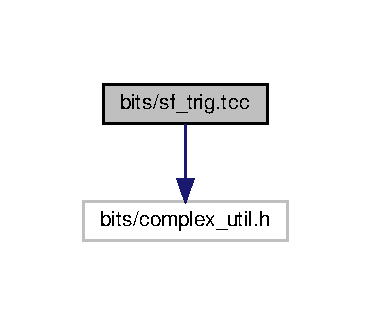
\includegraphics[width=178pt]{sf__trig_8tcc__incl}
\end{center}
\end{figure}
This graph shows which files directly or indirectly include this file\+:
\nopagebreak
\begin{figure}[H]
\begin{center}
\leavevmode
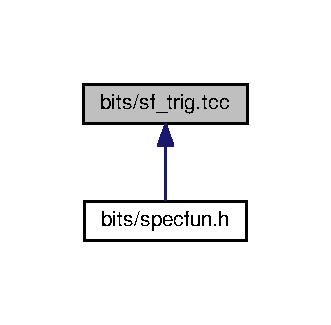
\includegraphics[width=159pt]{sf__trig_8tcc__dep__incl}
\end{center}
\end{figure}
\subsection*{Namespaces}
\begin{DoxyCompactItemize}
\item 
 \hyperlink{namespacestd}{std}
\item 
 \hyperlink{namespacestd_1_1____detail}{std\+::\+\_\+\+\_\+detail}
\begin{DoxyCompactList}\small\item\em Implementation-\/space details. \end{DoxyCompactList}\end{DoxyCompactItemize}
\subsection*{Macros}
\begin{DoxyCompactItemize}
\item 
\#define \hyperlink{sf__trig_8tcc_a6e1b0eff1758b4646af73ac467f1b629}{\+\_\+\+G\+L\+I\+B\+C\+X\+X\+\_\+\+B\+I\+T\+S\+\_\+\+S\+F\+\_\+\+T\+R\+I\+G\+\_\+\+T\+CC}~1
\end{DoxyCompactItemize}
\subsection*{Functions}
\begin{DoxyCompactItemize}
\item 
{\footnotesize template$<$typename \+\_\+\+Tp $>$ }\\\+\_\+\+Tp \hyperlink{namespacestd_1_1____detail_abfdaa500e1321747a0ad391ca3416a0b}{std\+::\+\_\+\+\_\+detail\+::\+\_\+\+\_\+cos\+\_\+pi} (\+\_\+\+Tp \+\_\+\+\_\+x)
\item 
{\footnotesize template$<$typename \+\_\+\+Tp $>$ }\\std\+::complex$<$ \+\_\+\+Tp $>$ \hyperlink{namespacestd_1_1____detail_a0332c7fb29ed7be543103adc8d04d39d}{std\+::\+\_\+\+\_\+detail\+::\+\_\+\+\_\+cos\+\_\+pi} (std\+::complex$<$ \+\_\+\+Tp $>$ \+\_\+\+\_\+z)
\item 
{\footnotesize template$<$typename \+\_\+\+Tp $>$ }\\\+\_\+\+Tp \hyperlink{namespacestd_1_1____detail_ae6e440447e88191b3cd19daaf7fda96e}{std\+::\+\_\+\+\_\+detail\+::\+\_\+\+\_\+cosh\+\_\+pi} (\+\_\+\+Tp \+\_\+\+\_\+x)
\item 
{\footnotesize template$<$typename \+\_\+\+Tp $>$ }\\std\+::complex$<$ \+\_\+\+Tp $>$ \hyperlink{namespacestd_1_1____detail_a257e13bd4fa9711a87ea68a783ee40d9}{std\+::\+\_\+\+\_\+detail\+::\+\_\+\+\_\+cosh\+\_\+pi} (std\+::complex$<$ \+\_\+\+Tp $>$ \+\_\+\+\_\+z)
\item 
{\footnotesize template$<$typename \+\_\+\+Tp $>$ }\\std\+::complex$<$ \+\_\+\+Tp $>$ \hyperlink{namespacestd_1_1____detail_ac69e259ad511fcc7a54c6ec315adcfa4}{std\+::\+\_\+\+\_\+detail\+::\+\_\+\+\_\+polar\+\_\+pi} (\+\_\+\+Tp \+\_\+\+\_\+rho, \+\_\+\+Tp \+\_\+\+\_\+phi\+\_\+pi)
\item 
{\footnotesize template$<$typename \+\_\+\+Tp $>$ }\\std\+::complex$<$ \+\_\+\+Tp $>$ \hyperlink{namespacestd_1_1____detail_a627c0e19f6b3e90af25735f351662d53}{std\+::\+\_\+\+\_\+detail\+::\+\_\+\+\_\+polar\+\_\+pi} (\+\_\+\+Tp \+\_\+\+\_\+rho, const std\+::complex$<$ \+\_\+\+Tp $>$ \&\+\_\+\+\_\+phi\+\_\+pi)
\item 
{\footnotesize template$<$typename \+\_\+\+Tp $>$ }\\\+\_\+\+Tp \hyperlink{namespacestd_1_1____detail_a763249defff6377195818c2fc6e7bca2}{std\+::\+\_\+\+\_\+detail\+::\+\_\+\+\_\+sin\+\_\+pi} (\+\_\+\+Tp \+\_\+\+\_\+x)
\item 
{\footnotesize template$<$typename \+\_\+\+Tp $>$ }\\std\+::complex$<$ \+\_\+\+Tp $>$ \hyperlink{namespacestd_1_1____detail_a5f26e85b3d646e5c69be173baebd4185}{std\+::\+\_\+\+\_\+detail\+::\+\_\+\+\_\+sin\+\_\+pi} (std\+::complex$<$ \+\_\+\+Tp $>$ \+\_\+\+\_\+z)
\item 
{\footnotesize template$<$typename \+\_\+\+Tp $>$ }\\\hyperlink{struct____gnu__cxx_1_1____sincos__t}{\+\_\+\+\_\+gnu\+\_\+cxx\+::\+\_\+\+\_\+sincos\+\_\+t}$<$ \+\_\+\+Tp $>$ \hyperlink{namespacestd_1_1____detail_a59a9ff6922faa1a88da8b485ee9d37cb}{std\+::\+\_\+\+\_\+detail\+::\+\_\+\+\_\+sincos} (\+\_\+\+Tp \+\_\+\+\_\+x)
\item 
{\footnotesize template$<$$>$ }\\\hyperlink{struct____gnu__cxx_1_1____sincos__t}{\+\_\+\+\_\+gnu\+\_\+cxx\+::\+\_\+\+\_\+sincos\+\_\+t}$<$ float $>$ \hyperlink{namespacestd_1_1____detail_a8cfd8b8345ebc359e31ac1631e29aeea}{std\+::\+\_\+\+\_\+detail\+::\+\_\+\+\_\+sincos} (float \+\_\+\+\_\+x)
\item 
{\footnotesize template$<$$>$ }\\\hyperlink{struct____gnu__cxx_1_1____sincos__t}{\+\_\+\+\_\+gnu\+\_\+cxx\+::\+\_\+\+\_\+sincos\+\_\+t}$<$ double $>$ \hyperlink{namespacestd_1_1____detail_a76c185b3a0156ecf557afdbf552a8916}{std\+::\+\_\+\+\_\+detail\+::\+\_\+\+\_\+sincos} (double \+\_\+\+\_\+x)
\item 
{\footnotesize template$<$$>$ }\\\hyperlink{struct____gnu__cxx_1_1____sincos__t}{\+\_\+\+\_\+gnu\+\_\+cxx\+::\+\_\+\+\_\+sincos\+\_\+t}$<$ long double $>$ \hyperlink{namespacestd_1_1____detail_aade98e6318f4459f37e1f79f4c871cf6}{std\+::\+\_\+\+\_\+detail\+::\+\_\+\+\_\+sincos} (long double \+\_\+\+\_\+x)
\item 
{\footnotesize template$<$typename \+\_\+\+Tp $>$ }\\\hyperlink{struct____gnu__cxx_1_1____sincos__t}{\+\_\+\+\_\+gnu\+\_\+cxx\+::\+\_\+\+\_\+sincos\+\_\+t}$<$ \+\_\+\+Tp $>$ \hyperlink{namespacestd_1_1____detail_af17af8caca5ba47597cc314e93ba49cd}{std\+::\+\_\+\+\_\+detail\+::\+\_\+\+\_\+sincos\+\_\+pi} (\+\_\+\+Tp \+\_\+\+\_\+x)
\item 
{\footnotesize template$<$typename \+\_\+\+Tp $>$ }\\\+\_\+\+Tp \hyperlink{namespacestd_1_1____detail_a6dd7153012cc7885e76a47a5162981da}{std\+::\+\_\+\+\_\+detail\+::\+\_\+\+\_\+sinh\+\_\+pi} (\+\_\+\+Tp \+\_\+\+\_\+x)
\item 
{\footnotesize template$<$typename \+\_\+\+Tp $>$ }\\std\+::complex$<$ \+\_\+\+Tp $>$ \hyperlink{namespacestd_1_1____detail_aa8fe06b3d9584ea9c81b0349ba7eb2dc}{std\+::\+\_\+\+\_\+detail\+::\+\_\+\+\_\+sinh\+\_\+pi} (std\+::complex$<$ \+\_\+\+Tp $>$ \+\_\+\+\_\+z)
\item 
{\footnotesize template$<$typename \+\_\+\+Tp $>$ }\\\+\_\+\+Tp \hyperlink{namespacestd_1_1____detail_a72fd3b7fcf9f49ade9411d782e8dbe4e}{std\+::\+\_\+\+\_\+detail\+::\+\_\+\+\_\+tan\+\_\+pi} (\+\_\+\+Tp \+\_\+\+\_\+x)
\item 
{\footnotesize template$<$typename \+\_\+\+Tp $>$ }\\std\+::complex$<$ \+\_\+\+Tp $>$ \hyperlink{namespacestd_1_1____detail_ae19d579db4245c9c4e53a70a0513bb00}{std\+::\+\_\+\+\_\+detail\+::\+\_\+\+\_\+tan\+\_\+pi} (std\+::complex$<$ \+\_\+\+Tp $>$ \+\_\+\+\_\+z)
\item 
{\footnotesize template$<$typename \+\_\+\+Tp $>$ }\\\+\_\+\+Tp \hyperlink{namespacestd_1_1____detail_ab0c02d3c15b8297df52b74807f22169b}{std\+::\+\_\+\+\_\+detail\+::\+\_\+\+\_\+tanh\+\_\+pi} (\+\_\+\+Tp \+\_\+\+\_\+x)
\item 
{\footnotesize template$<$typename \+\_\+\+Tp $>$ }\\std\+::complex$<$ \+\_\+\+Tp $>$ \hyperlink{namespacestd_1_1____detail_a75775747d40813d5d54c0b7a7d0c39f0}{std\+::\+\_\+\+\_\+detail\+::\+\_\+\+\_\+tanh\+\_\+pi} (std\+::complex$<$ \+\_\+\+Tp $>$ \+\_\+\+\_\+z)
\end{DoxyCompactItemize}


\subsection{Detailed Description}
This is an internal header file, included by other library headers. You should not attempt to use it directly. 

\subsection{Macro Definition Documentation}
\mbox{\Hypertarget{sf__trig_8tcc_a6e1b0eff1758b4646af73ac467f1b629}\label{sf__trig_8tcc_a6e1b0eff1758b4646af73ac467f1b629}} 
\index{sf\+\_\+trig.\+tcc@{sf\+\_\+trig.\+tcc}!\+\_\+\+G\+L\+I\+B\+C\+X\+X\+\_\+\+B\+I\+T\+S\+\_\+\+S\+F\+\_\+\+T\+R\+I\+G\+\_\+\+T\+CC@{\+\_\+\+G\+L\+I\+B\+C\+X\+X\+\_\+\+B\+I\+T\+S\+\_\+\+S\+F\+\_\+\+T\+R\+I\+G\+\_\+\+T\+CC}}
\index{\+\_\+\+G\+L\+I\+B\+C\+X\+X\+\_\+\+B\+I\+T\+S\+\_\+\+S\+F\+\_\+\+T\+R\+I\+G\+\_\+\+T\+CC@{\+\_\+\+G\+L\+I\+B\+C\+X\+X\+\_\+\+B\+I\+T\+S\+\_\+\+S\+F\+\_\+\+T\+R\+I\+G\+\_\+\+T\+CC}!sf\+\_\+trig.\+tcc@{sf\+\_\+trig.\+tcc}}
\subsubsection{\texorpdfstring{\+\_\+\+G\+L\+I\+B\+C\+X\+X\+\_\+\+B\+I\+T\+S\+\_\+\+S\+F\+\_\+\+T\+R\+I\+G\+\_\+\+T\+CC}{\_GLIBCXX\_BITS\_SF\_TRIG\_TCC}}
{\footnotesize\ttfamily \#define \+\_\+\+G\+L\+I\+B\+C\+X\+X\+\_\+\+B\+I\+T\+S\+\_\+\+S\+F\+\_\+\+T\+R\+I\+G\+\_\+\+T\+CC~1}



Definition at line 31 of file sf\+\_\+trig.\+tcc.


\hypertarget{sf__trigint_8tcc}{}\section{sf\+\_\+trigint.\+tcc File Reference}
\label{sf__trigint_8tcc}\index{sf\+\_\+trigint.\+tcc@{sf\+\_\+trigint.\+tcc}}
{\ttfamily \#include $<$ext/math\+\_\+const.\+h$>$}\\*
Include dependency graph for sf\+\_\+trigint.\+tcc\+:\nopagebreak
\begin{figure}[H]
\begin{center}
\leavevmode
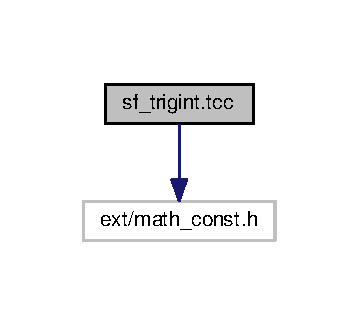
\includegraphics[width=172pt]{sf__trigint_8tcc__incl}
\end{center}
\end{figure}
\subsection*{Namespaces}
\begin{DoxyCompactItemize}
\item 
 \hyperlink{namespacestd}{std}
\item 
 \hyperlink{namespacestd_1_1____detail}{std\+::\+\_\+\+\_\+detail}
\end{DoxyCompactItemize}
\subsection*{Macros}
\begin{DoxyCompactItemize}
\item 
\#define \hyperlink{sf__trigint_8tcc_afde1ee684ded2155f3a3b305a31bb18e}{\+\_\+\+G\+L\+I\+B\+C\+X\+X\+\_\+\+S\+F\+\_\+\+T\+R\+I\+G\+I\+N\+T\+\_\+\+T\+C\+C}~1
\end{DoxyCompactItemize}
\subsection*{Enumerations}
\begin{DoxyCompactItemize}
\item 
enum \{ \hyperlink{namespacestd_1_1____detail_a354c633cb3e397eae4c31776b2d67923a0fef08e2967964a1421753c5d738c838}{std\+::\+\_\+\+\_\+detail\+::\+S\+I\+N\+I\+N\+T}, 
\hyperlink{namespacestd_1_1____detail_a354c633cb3e397eae4c31776b2d67923a4b5ea0190e37e477a2874e231190489e}{std\+::\+\_\+\+\_\+detail\+::\+C\+O\+S\+I\+N\+T}
 \}
\end{DoxyCompactItemize}
\subsection*{Functions}
\begin{DoxyCompactItemize}
\item 
{\footnotesize template$<$typename \+\_\+\+Tp $>$ }\\std\+::pair$<$ \+\_\+\+Tp, \+\_\+\+Tp $>$ \hyperlink{namespacestd_1_1____detail_a53bf807a99eef68cdb6f917c7ca085bf}{std\+::\+\_\+\+\_\+detail\+::\+\_\+\+\_\+sincosint} (\+\_\+\+Tp \+\_\+\+\_\+x)
\begin{DoxyCompactList}\small\item\em This function returns the sine $ Si(x) $ and cosine $ Ci(x) $ integrals as a {\ttfamily pair}. \end{DoxyCompactList}\item 
{\footnotesize template$<$typename \+\_\+\+Tp $>$ }\\void \hyperlink{namespacestd_1_1____detail_a976c3ff52c54001de3d409900c9bcb9c}{std\+::\+\_\+\+\_\+detail\+::\+\_\+\+\_\+sincosint\+\_\+asymp} (\+\_\+\+Tp \+\_\+\+\_\+t, \+\_\+\+Tp \&\+\_\+\+Si, \+\_\+\+Tp \&\+\_\+\+Ci)
\begin{DoxyCompactList}\small\item\em This function computes the sine $ Si(x) $ and cosine $ Ci(x) $ integrals by asymptotic series summation for positive argument. \end{DoxyCompactList}\item 
{\footnotesize template$<$typename \+\_\+\+Tp $>$ }\\void \hyperlink{namespacestd_1_1____detail_a211f552bca2944f64e3a1f5593690fda}{std\+::\+\_\+\+\_\+detail\+::\+\_\+\+\_\+sincosint\+\_\+cont\+\_\+frac} (\+\_\+\+Tp \+\_\+\+\_\+t, \+\_\+\+Tp \&\+\_\+\+Si, \+\_\+\+Tp \&\+\_\+\+Ci)
\begin{DoxyCompactList}\small\item\em This function computes the sine $ Si(x) $ and cosine $ Ci(x) $ integrals by continued fraction for positive argument. \end{DoxyCompactList}\item 
{\footnotesize template$<$typename \+\_\+\+Tp $>$ }\\void \hyperlink{namespacestd_1_1____detail_aea85e0044476065ed4a067f1aa9647cb}{std\+::\+\_\+\+\_\+detail\+::\+\_\+\+\_\+sincosint\+\_\+series} (\+\_\+\+Tp \+\_\+\+\_\+t, \+\_\+\+Tp \&\+\_\+\+Si, \+\_\+\+Tp \&\+\_\+\+Ci)
\begin{DoxyCompactList}\small\item\em This function computes the sine $ Si(x) $ and cosine $ Ci(x) $ integrals by series summation for positive argument. \end{DoxyCompactList}\end{DoxyCompactItemize}


\subsection{Macro Definition Documentation}
\hypertarget{sf__trigint_8tcc_afde1ee684ded2155f3a3b305a31bb18e}{}\index{sf\+\_\+trigint.\+tcc@{sf\+\_\+trigint.\+tcc}!\+\_\+\+G\+L\+I\+B\+C\+X\+X\+\_\+\+S\+F\+\_\+\+T\+R\+I\+G\+I\+N\+T\+\_\+\+T\+C\+C@{\+\_\+\+G\+L\+I\+B\+C\+X\+X\+\_\+\+S\+F\+\_\+\+T\+R\+I\+G\+I\+N\+T\+\_\+\+T\+C\+C}}
\index{\+\_\+\+G\+L\+I\+B\+C\+X\+X\+\_\+\+S\+F\+\_\+\+T\+R\+I\+G\+I\+N\+T\+\_\+\+T\+C\+C@{\+\_\+\+G\+L\+I\+B\+C\+X\+X\+\_\+\+S\+F\+\_\+\+T\+R\+I\+G\+I\+N\+T\+\_\+\+T\+C\+C}!sf\+\_\+trigint.\+tcc@{sf\+\_\+trigint.\+tcc}}
\subsubsection[{\+\_\+\+G\+L\+I\+B\+C\+X\+X\+\_\+\+S\+F\+\_\+\+T\+R\+I\+G\+I\+N\+T\+\_\+\+T\+C\+C}]{\setlength{\rightskip}{0pt plus 5cm}\#define \+\_\+\+G\+L\+I\+B\+C\+X\+X\+\_\+\+S\+F\+\_\+\+T\+R\+I\+G\+I\+N\+T\+\_\+\+T\+C\+C~1}\label{sf__trigint_8tcc_afde1ee684ded2155f3a3b305a31bb18e}


Definition at line 31 of file sf\+\_\+trigint.\+tcc.


\hypertarget{sf__zeta_8tcc}{}\section{bits/sf\+\_\+zeta.tcc File Reference}
\label{sf__zeta_8tcc}\index{bits/sf\+\_\+zeta.\+tcc@{bits/sf\+\_\+zeta.\+tcc}}
{\ttfamily \#include $<$ext/math\+\_\+const.\+h$>$}\\*
Include dependency graph for sf\+\_\+zeta.\+tcc\+:
\nopagebreak
\begin{figure}[H]
\begin{center}
\leavevmode
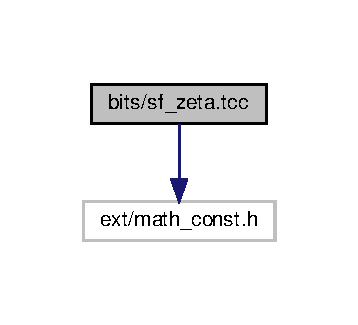
\includegraphics[width=172pt]{sf__zeta_8tcc__incl}
\end{center}
\end{figure}
This graph shows which files directly or indirectly include this file\+:
\nopagebreak
\begin{figure}[H]
\begin{center}
\leavevmode
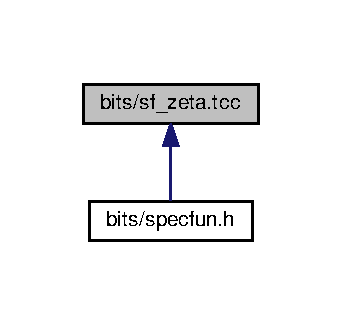
\includegraphics[width=164pt]{sf__zeta_8tcc__dep__incl}
\end{center}
\end{figure}
\subsection*{Namespaces}
\begin{DoxyCompactItemize}
\item 
 \hyperlink{namespacestd}{std}
\item 
 \hyperlink{namespacestd_1_1____detail}{std\+::\+\_\+\+\_\+detail}
\end{DoxyCompactItemize}
\subsection*{Macros}
\begin{DoxyCompactItemize}
\item 
\#define \hyperlink{sf__zeta_8tcc_a23ad81fae0dc2d916125d596553c5dfc}{\+\_\+\+G\+L\+I\+B\+C\+X\+X\+\_\+\+B\+I\+T\+S\+\_\+\+S\+F\+\_\+\+Z\+E\+T\+A\+\_\+\+T\+CC}~1
\end{DoxyCompactItemize}
\subsection*{Functions}
\begin{DoxyCompactItemize}
\item 
{\footnotesize template$<$typename \+\_\+\+Tp $>$ }\\\+\_\+\+Tp \hyperlink{namespacestd_1_1____detail_a26d3f285cfbcaba6fa30d3e4164c6187}{std\+::\+\_\+\+\_\+detail\+::\+\_\+\+\_\+debye} (unsigned int \+\_\+\+\_\+n, \+\_\+\+Tp \+\_\+\+\_\+x)
\item 
{\footnotesize template$<$typename \+\_\+\+Tp $>$ }\\\+\_\+\+Tp \hyperlink{namespacestd_1_1____detail_a5083a0c9fce3299593ca22e7dbaeaf19}{std\+::\+\_\+\+\_\+detail\+::\+\_\+\+\_\+dilog} (\+\_\+\+Tp \+\_\+\+\_\+x)
\begin{DoxyCompactList}\small\item\em Compute the dilogarithm function $ Li_2(x) $ by summation for x $<$= 1. \end{DoxyCompactList}\item 
{\footnotesize template$<$typename \+\_\+\+Tp $>$ }\\\+\_\+\+Tp \hyperlink{namespacestd_1_1____detail_a63aafed798ada71b2cc58e84a6652169}{std\+::\+\_\+\+\_\+detail\+::\+\_\+\+\_\+hurwitz\+\_\+zeta} (\+\_\+\+Tp \+\_\+\+\_\+s, \+\_\+\+Tp \+\_\+\+\_\+a)
\begin{DoxyCompactList}\small\item\em Return the Hurwitz zeta function $ \zeta(s,a) $ for all s != 1 and a $>$ -\/1. \end{DoxyCompactList}\item 
{\footnotesize template$<$typename \+\_\+\+Tp $>$ }\\\+\_\+\+Tp \hyperlink{namespacestd_1_1____detail_a56c55858723fe9e0c541f0e77572b58d}{std\+::\+\_\+\+\_\+detail\+::\+\_\+\+\_\+hurwitz\+\_\+zeta\+\_\+euler\+\_\+maclaurin} (\+\_\+\+Tp \+\_\+\+\_\+s, \+\_\+\+Tp \+\_\+\+\_\+a)
\begin{DoxyCompactList}\small\item\em Return the Hurwitz zeta function $ \zeta(s,a) $ for all s != 1 and a $>$ -\/1. \end{DoxyCompactList}\item 
{\footnotesize template$<$typename \+\_\+\+Tp $>$ }\\\+\_\+\+Tp \hyperlink{namespacestd_1_1____detail_a2be77d9bdd1b8b463be44a0e7558bc2a}{std\+::\+\_\+\+\_\+detail\+::\+\_\+\+\_\+riemann\+\_\+zeta} (\+\_\+\+Tp \+\_\+\+\_\+s)
\begin{DoxyCompactList}\small\item\em Return the Riemann zeta function $ \zeta(s) $. \end{DoxyCompactList}\item 
{\footnotesize template$<$typename \+\_\+\+Tp $>$ }\\\+\_\+\+Tp \hyperlink{namespacestd_1_1____detail_a84ac805996c4eeb8cbfa181e6e47f0ae}{std\+::\+\_\+\+\_\+detail\+::\+\_\+\+\_\+riemann\+\_\+zeta\+\_\+euler\+\_\+maclaurin} (\+\_\+\+Tp \+\_\+\+\_\+s)
\begin{DoxyCompactList}\small\item\em Evaluate the Riemann zeta function $ \zeta(s) $ by an alternate series for s $>$ 0. \end{DoxyCompactList}\item 
{\footnotesize template$<$typename \+\_\+\+Tp $>$ }\\\+\_\+\+Tp \hyperlink{namespacestd_1_1____detail_ab3542ea44b34da3d4865ed9a014e2951}{std\+::\+\_\+\+\_\+detail\+::\+\_\+\+\_\+riemann\+\_\+zeta\+\_\+glob} (\+\_\+\+Tp \+\_\+\+\_\+s)
\item 
{\footnotesize template$<$typename \+\_\+\+Tp $>$ }\\\+\_\+\+Tp \hyperlink{namespacestd_1_1____detail_a174bfa28eeb176b90ff251b5affbecb2}{std\+::\+\_\+\+\_\+detail\+::\+\_\+\+\_\+riemann\+\_\+zeta\+\_\+m\+\_\+1} (\+\_\+\+Tp \+\_\+\+\_\+s)
\begin{DoxyCompactList}\small\item\em Return the Riemann zeta function $ \zeta(s) - 1 $. \end{DoxyCompactList}\item 
{\footnotesize template$<$typename \+\_\+\+Tp $>$ }\\\+\_\+\+Tp \hyperlink{namespacestd_1_1____detail_ac7a15aa2658fef76642cebd7858fa0ff}{std\+::\+\_\+\+\_\+detail\+::\+\_\+\+\_\+riemann\+\_\+zeta\+\_\+m\+\_\+1\+\_\+glob} (\+\_\+\+Tp \+\_\+\+\_\+s)
\begin{DoxyCompactList}\small\item\em Evaluate the Riemann zeta function by series for all s != 1. Convergence is great until largish negative numbers. Then the convergence of the $>$ 0 sum gets better. \end{DoxyCompactList}\item 
{\footnotesize template$<$typename \+\_\+\+Tp $>$ }\\\+\_\+\+Tp \hyperlink{namespacestd_1_1____detail_a917935f42a21af90b78a19ea81349129}{std\+::\+\_\+\+\_\+detail\+::\+\_\+\+\_\+riemann\+\_\+zeta\+\_\+product} (\+\_\+\+Tp \+\_\+\+\_\+s)
\begin{DoxyCompactList}\small\item\em Compute the Riemann zeta function $ \zeta(s) $ using the product over prime factors. \end{DoxyCompactList}\item 
{\footnotesize template$<$typename \+\_\+\+Tp $>$ }\\\+\_\+\+Tp \hyperlink{namespacestd_1_1____detail_a417dc216465f02bb7ef055fa0e4e1f0b}{std\+::\+\_\+\+\_\+detail\+::\+\_\+\+\_\+riemann\+\_\+zeta\+\_\+sum} (\+\_\+\+Tp \+\_\+\+\_\+s)
\begin{DoxyCompactList}\small\item\em Compute the Riemann zeta function $ \zeta(s) $ by summation for s $>$ 1. \end{DoxyCompactList}\end{DoxyCompactItemize}
\subsection*{Variables}
\begin{DoxyCompactItemize}
\item 
constexpr size\+\_\+t \hyperlink{namespacestd_1_1____detail_ab27e687e1052be7a72de187e0dead124}{std\+::\+\_\+\+\_\+detail\+::\+\_\+\+Num\+\_\+\+Euler\+\_\+\+Maclaurin\+\_\+zeta} = 100
\item 
constexpr long double \hyperlink{namespacestd_1_1____detail_acd941b49595dd03e93c88107ad2f68c2}{std\+::\+\_\+\+\_\+detail\+::\+\_\+\+S\+\_\+\+Euler\+\_\+\+Maclaurin\+\_\+zeta} \mbox{[}\+\_\+\+Num\+\_\+\+Euler\+\_\+\+Maclaurin\+\_\+zeta\mbox{]}
\item 
constexpr size\+\_\+t \hyperlink{namespacestd_1_1____detail_a807e36c2aec3a9f27fdb21726cd464e2}{std\+::\+\_\+\+\_\+detail\+::\+\_\+\+S\+\_\+num\+\_\+zetam1} = 121
\item 
constexpr long double \hyperlink{namespacestd_1_1____detail_a22ed80d9e5c3bc79e61a3cdb8e79a462}{std\+::\+\_\+\+\_\+detail\+::\+\_\+\+S\+\_\+zetam1} \mbox{[}\+\_\+\+S\+\_\+num\+\_\+zetam1\mbox{]}
\end{DoxyCompactItemize}


\subsection{Detailed Description}
This is an internal header file, included by other library headers. Do not attempt to use it directly. Instead, include $<$cmath$>$. 

\subsection{Macro Definition Documentation}
\index{sf\+\_\+zeta.\+tcc@{sf\+\_\+zeta.\+tcc}!\+\_\+\+G\+L\+I\+B\+C\+X\+X\+\_\+\+B\+I\+T\+S\+\_\+\+S\+F\+\_\+\+Z\+E\+T\+A\+\_\+\+T\+CC@{\+\_\+\+G\+L\+I\+B\+C\+X\+X\+\_\+\+B\+I\+T\+S\+\_\+\+S\+F\+\_\+\+Z\+E\+T\+A\+\_\+\+T\+CC}}
\index{\+\_\+\+G\+L\+I\+B\+C\+X\+X\+\_\+\+B\+I\+T\+S\+\_\+\+S\+F\+\_\+\+Z\+E\+T\+A\+\_\+\+T\+CC@{\+\_\+\+G\+L\+I\+B\+C\+X\+X\+\_\+\+B\+I\+T\+S\+\_\+\+S\+F\+\_\+\+Z\+E\+T\+A\+\_\+\+T\+CC}!sf\+\_\+zeta.\+tcc@{sf\+\_\+zeta.\+tcc}}
\subsubsection[{\texorpdfstring{\+\_\+\+G\+L\+I\+B\+C\+X\+X\+\_\+\+B\+I\+T\+S\+\_\+\+S\+F\+\_\+\+Z\+E\+T\+A\+\_\+\+T\+CC}{_GLIBCXX_BITS_SF_ZETA_TCC}}]{\setlength{\rightskip}{0pt plus 5cm}\#define \+\_\+\+G\+L\+I\+B\+C\+X\+X\+\_\+\+B\+I\+T\+S\+\_\+\+S\+F\+\_\+\+Z\+E\+T\+A\+\_\+\+T\+CC~1}\hypertarget{sf__zeta_8tcc_a23ad81fae0dc2d916125d596553c5dfc}{}\label{sf__zeta_8tcc_a23ad81fae0dc2d916125d596553c5dfc}


Definition at line 46 of file sf\+\_\+zeta.\+tcc.


\hypertarget{specfun_8h}{}\section{bits/specfun.h File Reference}
\label{specfun_8h}\index{bits/specfun.\+h@{bits/specfun.\+h}}
{\ttfamily \#include $<$bits/c++config.\+h$>$}\\*
{\ttfamily \#include $<$limits$>$}\\*
{\ttfamily \#include $<$bits/stl\+\_\+algobase.\+h$>$}\\*
{\ttfamily \#include $<$bits/specfun\+\_\+util.\+h$>$}\\*
{\ttfamily \#include $<$type\+\_\+traits$>$}\\*
{\ttfamily \#include $<$bits/numeric\+\_\+limits.\+h$>$}\\*
{\ttfamily \#include $<$bits/complex\+\_\+util.\+h$>$}\\*
{\ttfamily \#include $<$bits/sf\+\_\+gamma.\+tcc$>$}\\*
{\ttfamily \#include $<$bits/sf\+\_\+bessel.\+tcc$>$}\\*
{\ttfamily \#include $<$bits/sf\+\_\+beta.\+tcc$>$}\\*
{\ttfamily \#include $<$bits/sf\+\_\+cardinal.\+tcc$>$}\\*
{\ttfamily \#include $<$bits/sf\+\_\+chebyshev.\+tcc$>$}\\*
{\ttfamily \#include $<$bits/sf\+\_\+dawson.\+tcc$>$}\\*
{\ttfamily \#include $<$bits/sf\+\_\+ellint.\+tcc$>$}\\*
{\ttfamily \#include $<$bits/sf\+\_\+expint.\+tcc$>$}\\*
{\ttfamily \#include $<$bits/sf\+\_\+fresnel.\+tcc$>$}\\*
{\ttfamily \#include $<$bits/sf\+\_\+gegenbauer.\+tcc$>$}\\*
{\ttfamily \#include $<$bits/sf\+\_\+hyperg.\+tcc$>$}\\*
{\ttfamily \#include $<$bits/sf\+\_\+hypint.\+tcc$>$}\\*
{\ttfamily \#include $<$bits/sf\+\_\+jacobi.\+tcc$>$}\\*
{\ttfamily \#include $<$bits/sf\+\_\+laguerre.\+tcc$>$}\\*
{\ttfamily \#include $<$bits/sf\+\_\+legendre.\+tcc$>$}\\*
{\ttfamily \#include $<$bits/sf\+\_\+hydrogen.\+tcc$>$}\\*
{\ttfamily \#include $<$bits/sf\+\_\+mod\+\_\+bessel.\+tcc$>$}\\*
{\ttfamily \#include $<$bits/sf\+\_\+hermite.\+tcc$>$}\\*
{\ttfamily \#include $<$bits/sf\+\_\+theta.\+tcc$>$}\\*
{\ttfamily \#include $<$bits/sf\+\_\+trigint.\+tcc$>$}\\*
{\ttfamily \#include $<$bits/sf\+\_\+zeta.\+tcc$>$}\\*
{\ttfamily \#include $<$bits/sf\+\_\+owens\+\_\+t.\+tcc$>$}\\*
{\ttfamily \#include $<$bits/sf\+\_\+polylog.\+tcc$>$}\\*
{\ttfamily \#include $<$bits/sf\+\_\+airy.\+tcc$>$}\\*
{\ttfamily \#include $<$bits/sf\+\_\+hankel.\+tcc$>$}\\*
{\ttfamily \#include $<$bits/sf\+\_\+distributions.\+tcc$>$}\\*
Include dependency graph for specfun.\+h\+:
\nopagebreak
\begin{figure}[H]
\begin{center}
\leavevmode

\includegraphics[width=350pt]{specfun_8h__incl}
\end{center}
\end{figure}
\subsection*{Namespaces}
\begin{DoxyCompactItemize}
\item 
 \hyperlink{namespace____gnu__cxx}{\+\_\+\+\_\+gnu\+\_\+cxx}
\item 
 \hyperlink{namespacestd}{std}
\end{DoxyCompactItemize}
\subsection*{Macros}
\begin{DoxyCompactItemize}
\item 
\#define \hyperlink{specfun_8h_ad3219e2507c3e671381bd3d2b67be6e4}{\+\_\+\+\_\+cpp\+\_\+lib\+\_\+math\+\_\+special\+\_\+functions}~201603L
\item 
\#define \hyperlink{specfun_8h_a58f485f9da6a45af06142aeeb575457b}{\+\_\+\+\_\+\+S\+T\+D\+C\+P\+P\+\_\+\+M\+A\+T\+H\+\_\+\+S\+P\+E\+C\+\_\+\+F\+U\+N\+C\+S\+\_\+\+\_\+}~201003L
\end{DoxyCompactItemize}
\subsection*{Enumerations}
\begin{DoxyCompactItemize}
\item 
enum \{ \hyperlink{group__gnu__math__spec__func_ggad6c62dd86a596716cece6ac2d4cfd4b3a3f3a4942031777493cbc33f592c941c7}{\+\_\+\+\_\+gnu\+\_\+cxx\+::\+\_\+\+G\+L\+I\+B\+C\+X\+X\+\_\+\+J\+A\+C\+O\+B\+I\+\_\+\+SN}, 
\hyperlink{group__gnu__math__spec__func_ggad6c62dd86a596716cece6ac2d4cfd4b3a86d36c2efbbbfddcfb1e552853d72d65}{\+\_\+\+\_\+gnu\+\_\+cxx\+::\+\_\+\+G\+L\+I\+B\+C\+X\+X\+\_\+\+J\+A\+C\+O\+B\+I\+\_\+\+CN}, 
\hyperlink{group__gnu__math__spec__func_ggad6c62dd86a596716cece6ac2d4cfd4b3a4576182edcbe93595def76dd1e61e0f7}{\+\_\+\+\_\+gnu\+\_\+cxx\+::\+\_\+\+G\+L\+I\+B\+C\+X\+X\+\_\+\+J\+A\+C\+O\+B\+I\+\_\+\+DN}
 \}
\end{DoxyCompactItemize}
\subsection*{Functions}
\begin{DoxyCompactItemize}
\item 
{\footnotesize template$<$typename \+\_\+\+Tp $>$ }\\\+\_\+\+\_\+gnu\+\_\+cxx\+::\+\_\+\+\_\+promote\+\_\+num\+\_\+t$<$ \+\_\+\+Tp $>$ \hyperlink{group__gnu__math__spec__func_ga8eff81346e95e9987002ea52fe1e29a7}{\+\_\+\+\_\+gnu\+\_\+cxx\+::airy\+\_\+ai} (\+\_\+\+Tp \+\_\+\+\_\+x)
\item 
float \hyperlink{group__gnu__math__spec__func_gaf317ba724c44b3a8271fe341d9870173}{\+\_\+\+\_\+gnu\+\_\+cxx\+::airy\+\_\+aif} (float \+\_\+\+\_\+x)
\item 
long double \hyperlink{group__gnu__math__spec__func_ga800fdb61c672ae1831f4ca4250d657de}{\+\_\+\+\_\+gnu\+\_\+cxx\+::airy\+\_\+ail} (long double \+\_\+\+\_\+x)
\item 
{\footnotesize template$<$typename \+\_\+\+Tp $>$ }\\\+\_\+\+\_\+gnu\+\_\+cxx\+::\+\_\+\+\_\+promote\+\_\+num\+\_\+t$<$ \+\_\+\+Tp $>$ \hyperlink{group__gnu__math__spec__func_ga65253611eb5aec804f9021b085be2a48}{\+\_\+\+\_\+gnu\+\_\+cxx\+::airy\+\_\+bi} (\+\_\+\+Tp \+\_\+\+\_\+x)
\item 
float \hyperlink{group__gnu__math__spec__func_ga2ade465827bdba7370abbcce78e54912}{\+\_\+\+\_\+gnu\+\_\+cxx\+::airy\+\_\+bif} (float \+\_\+\+\_\+x)
\item 
long double \hyperlink{group__gnu__math__spec__func_ga59240b3f40177e5187f3f194f624f0f8}{\+\_\+\+\_\+gnu\+\_\+cxx\+::airy\+\_\+bil} (long double \+\_\+\+\_\+x)
\item 
{\footnotesize template$<$typename \+\_\+\+Tp $>$ }\\\+\_\+\+\_\+gnu\+\_\+cxx\+::\+\_\+\+\_\+promote$<$ \+\_\+\+Tp $>$\+::\+\_\+\+\_\+type \hyperlink{group__tr29124__math__spec__func_ga377bb7e038c464a27dfe0573fd2d7b33}{std\+::assoc\+\_\+laguerre} (unsigned int \+\_\+\+\_\+n, unsigned int \+\_\+\+\_\+m, \+\_\+\+Tp \+\_\+\+\_\+x)
\item 
float \hyperlink{group__tr29124__math__spec__func_gaf83d98f350a1cfcebee6a1f723cf90d2}{std\+::assoc\+\_\+laguerref} (unsigned int \+\_\+\+\_\+n, unsigned int \+\_\+\+\_\+m, float \+\_\+\+\_\+x)
\item 
long double \hyperlink{group__tr29124__math__spec__func_gac8e245671fb2df5de5fd978d03081f6c}{std\+::assoc\+\_\+laguerrel} (unsigned int \+\_\+\+\_\+n, unsigned int \+\_\+\+\_\+m, long double \+\_\+\+\_\+x)
\item 
{\footnotesize template$<$typename \+\_\+\+Tp $>$ }\\\+\_\+\+\_\+gnu\+\_\+cxx\+::\+\_\+\+\_\+promote$<$ \+\_\+\+Tp $>$\+::\+\_\+\+\_\+type \hyperlink{group__tr29124__math__spec__func_ga355349f79119c1fd1e2a9351cec57f0f}{std\+::assoc\+\_\+legendre} (unsigned int \+\_\+\+\_\+l, unsigned int \+\_\+\+\_\+m, \+\_\+\+Tp \+\_\+\+\_\+x)
\item 
float \hyperlink{group__tr29124__math__spec__func_ga3ced07ddd24bf4af56e2712d148e7f57}{std\+::assoc\+\_\+legendref} (unsigned int \+\_\+\+\_\+l, unsigned int \+\_\+\+\_\+m, float \+\_\+\+\_\+x)
\item 
long double \hyperlink{group__tr29124__math__spec__func_ga55977b425a539146f060dec1c8003344}{std\+::assoc\+\_\+legendrel} (unsigned int \+\_\+\+\_\+l, unsigned int \+\_\+\+\_\+m, long double \+\_\+\+\_\+x)
\item 
{\footnotesize template$<$typename \+\_\+\+Tp $>$ }\\\+\_\+\+\_\+gnu\+\_\+cxx\+::\+\_\+\+\_\+promote\+\_\+num\+\_\+t$<$ \+\_\+\+Tp $>$ \hyperlink{group__gnu__math__spec__func_ga3fc87e918adf978bfdc26a182af0e6ed}{\+\_\+\+\_\+gnu\+\_\+cxx\+::bernoulli} (unsigned int \+\_\+\+\_\+n)
\item 
float \hyperlink{group__gnu__math__spec__func_gabcd77f012ae74989c4bb9ca61978481d}{\+\_\+\+\_\+gnu\+\_\+cxx\+::bernoullif} (unsigned int \+\_\+\+\_\+n)
\item 
long double \hyperlink{group__gnu__math__spec__func_gaac8f04abfdd6b744d11cb73ec1f564b1}{\+\_\+\+\_\+gnu\+\_\+cxx\+::bernoullil} (unsigned int \+\_\+\+\_\+n)
\item 
{\footnotesize template$<$typename \+\_\+\+Tpa , typename \+\_\+\+Tpb $>$ }\\\+\_\+\+\_\+gnu\+\_\+cxx\+::\+\_\+\+\_\+promote\+\_\+2$<$ \+\_\+\+Tpa, \+\_\+\+Tpb $>$\+::\+\_\+\+\_\+type \hyperlink{group__tr29124__math__spec__func_ga6a7220c87c942db48b18b527d92bbd2d}{std\+::beta} (\+\_\+\+Tpa \+\_\+\+\_\+a, \+\_\+\+Tpb \+\_\+\+\_\+b)
\item 
float \hyperlink{group__tr29124__math__spec__func_ga12dc61ee4c09172151cf092ed387e203}{std\+::betaf} (float \+\_\+\+\_\+a, float \+\_\+\+\_\+b)
\item 
long double \hyperlink{group__tr29124__math__spec__func_ga8caca1cef099f41a88111209c36ce06c}{std\+::betal} (long double \+\_\+\+\_\+a, long double \+\_\+\+\_\+b)
\item 
{\footnotesize template$<$typename \+\_\+\+Tp $>$ }\\\+\_\+\+\_\+gnu\+\_\+cxx\+::\+\_\+\+\_\+promote\+\_\+num\+\_\+t$<$ \+\_\+\+Tp $>$ \hyperlink{group__gnu__math__spec__func_ga57a15003ded8e0e808b21d4a17a7803e}{\+\_\+\+\_\+gnu\+\_\+cxx\+::bincoef} (unsigned int \+\_\+\+\_\+n, unsigned int \+\_\+\+\_\+k)
\item 
float \hyperlink{group__gnu__math__spec__func_ga20ff8c4c82808c78c299634d02f3f8bd}{\+\_\+\+\_\+gnu\+\_\+cxx\+::bincoeff} (unsigned int \+\_\+\+\_\+n, unsigned int \+\_\+\+\_\+k)
\item 
long double \hyperlink{group__gnu__math__spec__func_ga6874da4660b1ef35c03e28bf09e81796}{\+\_\+\+\_\+gnu\+\_\+cxx\+::bincoefl} (unsigned int \+\_\+\+\_\+n, unsigned int \+\_\+\+\_\+k)
\item 
{\footnotesize template$<$typename \+\_\+\+Tp $>$ }\\\+\_\+\+\_\+gnu\+\_\+cxx\+::\+\_\+\+\_\+promote\+\_\+num\+\_\+t$<$ \+\_\+\+Tp $>$ \hyperlink{group__gnu__math__spec__func_gad8769048d3a0eb2adcfcfeaa10af37fe}{\+\_\+\+\_\+gnu\+\_\+cxx\+::chebyshev\+\_\+t} (unsigned int \+\_\+\+\_\+n, \+\_\+\+Tp \+\_\+\+\_\+x)
\item 
float \hyperlink{group__gnu__math__spec__func_gab8cdb55702d9c8b85af4ecc3d8c6a134}{\+\_\+\+\_\+gnu\+\_\+cxx\+::chebyshev\+\_\+tf} (unsigned int \+\_\+\+\_\+n, float \+\_\+\+\_\+x)
\item 
long double \hyperlink{group__gnu__math__spec__func_ga0c421700d244cdf58e3ac5ff267664d1}{\+\_\+\+\_\+gnu\+\_\+cxx\+::chebyshev\+\_\+tl} (unsigned int \+\_\+\+\_\+n, long double \+\_\+\+\_\+x)
\item 
{\footnotesize template$<$typename \+\_\+\+Tp $>$ }\\\+\_\+\+\_\+gnu\+\_\+cxx\+::\+\_\+\+\_\+promote\+\_\+num\+\_\+t$<$ \+\_\+\+Tp $>$ \hyperlink{group__gnu__math__spec__func_ga59e3a6dd4d614f6e158a0a56fa25a0b1}{\+\_\+\+\_\+gnu\+\_\+cxx\+::chebyshev\+\_\+u} (unsigned int \+\_\+\+\_\+n, \+\_\+\+Tp \+\_\+\+\_\+x)
\item 
float \hyperlink{group__gnu__math__spec__func_ga4b28c2a079eae2e9612c9902801ca256}{\+\_\+\+\_\+gnu\+\_\+cxx\+::chebyshev\+\_\+uf} (unsigned int \+\_\+\+\_\+n, float \+\_\+\+\_\+x)
\item 
long double \hyperlink{group__gnu__math__spec__func_ga11ec202d6aacafba1182e962ecf02978}{\+\_\+\+\_\+gnu\+\_\+cxx\+::chebyshev\+\_\+ul} (unsigned int \+\_\+\+\_\+n, long double \+\_\+\+\_\+x)
\item 
{\footnotesize template$<$typename \+\_\+\+Tp $>$ }\\\+\_\+\+\_\+gnu\+\_\+cxx\+::\+\_\+\+\_\+promote\+\_\+num\+\_\+t$<$ \+\_\+\+Tp $>$ \hyperlink{group__gnu__math__spec__func_gaf5e47fa5f24acf2aac6c7a1187ee6be1}{\+\_\+\+\_\+gnu\+\_\+cxx\+::chebyshev\+\_\+v} (unsigned int \+\_\+\+\_\+n, \+\_\+\+Tp \+\_\+\+\_\+x)
\item 
float \hyperlink{group__gnu__math__spec__func_gaa9635a0da4bdeaa8060ae5cf03c3a12d}{\+\_\+\+\_\+gnu\+\_\+cxx\+::chebyshev\+\_\+vf} (unsigned int \+\_\+\+\_\+n, float \+\_\+\+\_\+x)
\item 
long double \hyperlink{group__gnu__math__spec__func_gae387ee1bfcd52555ad4d690f5888a078}{\+\_\+\+\_\+gnu\+\_\+cxx\+::chebyshev\+\_\+vl} (unsigned int \+\_\+\+\_\+n, long double \+\_\+\+\_\+x)
\item 
{\footnotesize template$<$typename \+\_\+\+Tp $>$ }\\\+\_\+\+\_\+gnu\+\_\+cxx\+::\+\_\+\+\_\+promote\+\_\+num\+\_\+t$<$ \+\_\+\+Tp $>$ \hyperlink{group__gnu__math__spec__func_gae283d165c5a058fff7a0f83a2a66b4c2}{\+\_\+\+\_\+gnu\+\_\+cxx\+::chebyshev\+\_\+w} (unsigned int \+\_\+\+\_\+n, \+\_\+\+Tp \+\_\+\+\_\+x)
\item 
float \hyperlink{group__gnu__math__spec__func_gae6d468cee53df584e40afe294127b090}{\+\_\+\+\_\+gnu\+\_\+cxx\+::chebyshev\+\_\+wf} (unsigned int \+\_\+\+\_\+n, float \+\_\+\+\_\+x)
\item 
long double \hyperlink{group__gnu__math__spec__func_ga1297dfd9b9a0f584435de7d83eb9e9c3}{\+\_\+\+\_\+gnu\+\_\+cxx\+::chebyshev\+\_\+wl} (unsigned int \+\_\+\+\_\+n, long double \+\_\+\+\_\+x)
\item 
{\footnotesize template$<$typename \+\_\+\+Tp $>$ }\\\+\_\+\+\_\+gnu\+\_\+cxx\+::\+\_\+\+\_\+promote\+\_\+num\+\_\+t$<$ \+\_\+\+Tp $>$ \hyperlink{group__gnu__math__spec__func_ga5a7016834baf2dd1b57c9dfcfa3436f0}{\+\_\+\+\_\+gnu\+\_\+cxx\+::clausen} (unsigned int \+\_\+\+\_\+m, \+\_\+\+Tp \+\_\+\+\_\+w)
\item 
{\footnotesize template$<$typename \+\_\+\+Tp $>$ }\\std\+::complex$<$ \+\_\+\+\_\+gnu\+\_\+cxx\+::\+\_\+\+\_\+promote\+\_\+num\+\_\+t$<$ \+\_\+\+Tp $>$ $>$ \hyperlink{group__gnu__math__spec__func_ga154f5baa4a7799557b7e7d32dfc73285}{\+\_\+\+\_\+gnu\+\_\+cxx\+::clausen} (unsigned int \+\_\+\+\_\+m, std\+::complex$<$ \+\_\+\+Tp $>$ \+\_\+\+\_\+w)
\item 
{\footnotesize template$<$typename \+\_\+\+Tp $>$ }\\\+\_\+\+\_\+gnu\+\_\+cxx\+::\+\_\+\+\_\+promote\+\_\+num\+\_\+t$<$ \+\_\+\+Tp $>$ \hyperlink{group__gnu__math__spec__func_ga2e89f9758322054738dacf686f6ce974}{\+\_\+\+\_\+gnu\+\_\+cxx\+::clausen\+\_\+c} (unsigned int \+\_\+\+\_\+m, \+\_\+\+Tp \+\_\+\+\_\+w)
\item 
float \hyperlink{group__gnu__math__spec__func_ga515b9b6bca8f97e696ac5be85a44b3bd}{\+\_\+\+\_\+gnu\+\_\+cxx\+::clausen\+\_\+cf} (unsigned int \+\_\+\+\_\+m, float \+\_\+\+\_\+w)
\item 
long double \hyperlink{group__gnu__math__spec__func_ga5ff89833dc529ca3de5099e1b9c8525f}{\+\_\+\+\_\+gnu\+\_\+cxx\+::clausen\+\_\+cl} (unsigned int \+\_\+\+\_\+m, long double \+\_\+\+\_\+w)
\item 
{\footnotesize template$<$typename \+\_\+\+Tp $>$ }\\\+\_\+\+\_\+gnu\+\_\+cxx\+::\+\_\+\+\_\+promote\+\_\+num\+\_\+t$<$ \+\_\+\+Tp $>$ \hyperlink{group__gnu__math__spec__func_ga124827c09e71d83eb11b9e3282739475}{\+\_\+\+\_\+gnu\+\_\+cxx\+::clausen\+\_\+s} (unsigned int \+\_\+\+\_\+m, \+\_\+\+Tp \+\_\+\+\_\+w)
\item 
float \hyperlink{group__gnu__math__spec__func_ga2308b5828b5a8003d16cfa0f90826f94}{\+\_\+\+\_\+gnu\+\_\+cxx\+::clausen\+\_\+sf} (unsigned int \+\_\+\+\_\+m, float \+\_\+\+\_\+w)
\item 
long double \hyperlink{group__gnu__math__spec__func_ga6eb205278e3807367b62e07c3f39d915}{\+\_\+\+\_\+gnu\+\_\+cxx\+::clausen\+\_\+sl} (unsigned int \+\_\+\+\_\+m, long double \+\_\+\+\_\+w)
\item 
float \hyperlink{group__gnu__math__spec__func_ga9e228490e55e7936f77ae7a5ef9821dc}{\+\_\+\+\_\+gnu\+\_\+cxx\+::clausenf} (unsigned int \+\_\+\+\_\+m, float \+\_\+\+\_\+w)
\item 
std\+::complex$<$ float $>$ \hyperlink{group__gnu__math__spec__func_ga769ee593c5f1c1d8148abb9bebe50821}{\+\_\+\+\_\+gnu\+\_\+cxx\+::clausenf} (unsigned int \+\_\+\+\_\+m, std\+::complex$<$ float $>$ \+\_\+\+\_\+w)
\item 
long double \hyperlink{group__gnu__math__spec__func_gaac0a4d039044c04cd26c9b8559c441fd}{\+\_\+\+\_\+gnu\+\_\+cxx\+::clausenl} (unsigned int \+\_\+\+\_\+m, long double \+\_\+\+\_\+w)
\item 
std\+::complex$<$ long double $>$ \hyperlink{group__gnu__math__spec__func_ga6e1e9929ace5a66d970c308554473a26}{\+\_\+\+\_\+gnu\+\_\+cxx\+::clausenl} (unsigned int \+\_\+\+\_\+m, std\+::complex$<$ long double $>$ \+\_\+\+\_\+w)
\item 
{\footnotesize template$<$typename \+\_\+\+Tp $>$ }\\\+\_\+\+\_\+gnu\+\_\+cxx\+::\+\_\+\+\_\+promote$<$ \+\_\+\+Tp $>$\+::\+\_\+\+\_\+type \hyperlink{group__tr29124__math__spec__func_gac559500c604c43ea943d593c9ad9d289}{std\+::comp\+\_\+ellint\+\_\+1} (\+\_\+\+Tp \+\_\+\+\_\+k)
\item 
float \hyperlink{group__tr29124__math__spec__func_ga7fb5be999a8125cf7e55e630eb8444a1}{std\+::comp\+\_\+ellint\+\_\+1f} (float \+\_\+\+\_\+k)
\item 
long double \hyperlink{group__tr29124__math__spec__func_ga7247d3dd77c1ff5df3c059fed862dc48}{std\+::comp\+\_\+ellint\+\_\+1l} (long double \+\_\+\+\_\+k)
\item 
{\footnotesize template$<$typename \+\_\+\+Tp $>$ }\\\+\_\+\+\_\+gnu\+\_\+cxx\+::\+\_\+\+\_\+promote$<$ \+\_\+\+Tp $>$\+::\+\_\+\+\_\+type \hyperlink{group__tr29124__math__spec__func_ga22fcc678829f0daf2de257896378e7e0}{std\+::comp\+\_\+ellint\+\_\+2} (\+\_\+\+Tp \+\_\+\+\_\+k)
\item 
float \hyperlink{group__tr29124__math__spec__func_ga21700f2f125c42b1f1da1f9c7eea1135}{std\+::comp\+\_\+ellint\+\_\+2f} (float \+\_\+\+\_\+k)
\item 
long double \hyperlink{group__tr29124__math__spec__func_ga47b647ec386c8d4b18a030c97842df18}{std\+::comp\+\_\+ellint\+\_\+2l} (long double \+\_\+\+\_\+k)
\item 
{\footnotesize template$<$typename \+\_\+\+Tp , typename \+\_\+\+Tpn $>$ }\\\+\_\+\+\_\+gnu\+\_\+cxx\+::\+\_\+\+\_\+promote\+\_\+2$<$ \+\_\+\+Tp, \+\_\+\+Tpn $>$\+::\+\_\+\+\_\+type \hyperlink{group__tr29124__math__spec__func_gad833404645e24b7f0598a640ff92d623}{std\+::comp\+\_\+ellint\+\_\+3} (\+\_\+\+Tp \+\_\+\+\_\+k, \+\_\+\+Tpn \+\_\+\+\_\+nu)
\item 
float \hyperlink{group__tr29124__math__spec__func_ga76834d3112f777703330892303267a39}{std\+::comp\+\_\+ellint\+\_\+3f} (float \+\_\+\+\_\+k, float \+\_\+\+\_\+nu)
\begin{DoxyCompactList}\small\item\em Return the complete elliptic integral of the third kind $ \Pi(k,\nu) $ for {\ttfamily float} modulus $ k $. \end{DoxyCompactList}\item 
long double \hyperlink{group__tr29124__math__spec__func_ga1ca081fee102cd0d4d6b091285e495e5}{std\+::comp\+\_\+ellint\+\_\+3l} (long double \+\_\+\+\_\+k, long double \+\_\+\+\_\+nu)
\begin{DoxyCompactList}\small\item\em Return the complete elliptic integral of the third kind $ \Pi(k,\nu) $ for {\ttfamily long double} modulus {\ttfamily k}. \end{DoxyCompactList}\item 
{\footnotesize template$<$typename \+\_\+\+Tk $>$ }\\\+\_\+\+\_\+gnu\+\_\+cxx\+::\+\_\+\+\_\+promote\+\_\+num\+\_\+t$<$ \+\_\+\+Tk $>$ \hyperlink{group__gnu__math__spec__func_gad0fb35dfc5aef8ba2ba5fb88da1192c7}{\+\_\+\+\_\+gnu\+\_\+cxx\+::comp\+\_\+ellint\+\_\+d} (\+\_\+\+Tk \+\_\+\+\_\+k)
\item 
float \hyperlink{group__gnu__math__spec__func_ga34ac6488b0e7531d5d4b7a8e31ff864e}{\+\_\+\+\_\+gnu\+\_\+cxx\+::comp\+\_\+ellint\+\_\+df} (float \+\_\+\+\_\+k)
\item 
long double \hyperlink{group__gnu__math__spec__func_ga494931ec0a271b79f1fdcfdf929e3138}{\+\_\+\+\_\+gnu\+\_\+cxx\+::comp\+\_\+ellint\+\_\+dl} (long double \+\_\+\+\_\+k)
\item 
float \hyperlink{group__gnu__math__spec__func_ga55ae30b4f8ff15017d18a80050e14e38}{\+\_\+\+\_\+gnu\+\_\+cxx\+::comp\+\_\+ellint\+\_\+rf} (float \+\_\+\+\_\+x, float \+\_\+\+\_\+y)
\item 
long double \hyperlink{group__gnu__math__spec__func_gae1d468487f1711e91719a9c6392f3c35}{\+\_\+\+\_\+gnu\+\_\+cxx\+::comp\+\_\+ellint\+\_\+rf} (long double \+\_\+\+\_\+x, long double \+\_\+\+\_\+y)
\item 
{\footnotesize template$<$typename \+\_\+\+Tx , typename \+\_\+\+Ty $>$ }\\\+\_\+\+\_\+gnu\+\_\+cxx\+::\+\_\+\+\_\+promote\+\_\+num\+\_\+t$<$ \+\_\+\+Tx, \+\_\+\+Ty $>$ \hyperlink{group__gnu__math__spec__func_ga98dd868dcb97e26971dfa8ac4db24df3}{\+\_\+\+\_\+gnu\+\_\+cxx\+::comp\+\_\+ellint\+\_\+rf} (\+\_\+\+Tx \+\_\+\+\_\+x, \+\_\+\+Ty \+\_\+\+\_\+y)
\item 
float \hyperlink{group__gnu__math__spec__func_ga978f8eec6e5edc918b243925dbacb65b}{\+\_\+\+\_\+gnu\+\_\+cxx\+::comp\+\_\+ellint\+\_\+rg} (float \+\_\+\+\_\+x, float \+\_\+\+\_\+y)
\item 
long double \hyperlink{group__gnu__math__spec__func_gaca5fa8ee8125afc8f35ec6b27806e873}{\+\_\+\+\_\+gnu\+\_\+cxx\+::comp\+\_\+ellint\+\_\+rg} (long double \+\_\+\+\_\+x, long double \+\_\+\+\_\+y)
\item 
{\footnotesize template$<$typename \+\_\+\+Tx , typename \+\_\+\+Ty $>$ }\\\+\_\+\+\_\+gnu\+\_\+cxx\+::\+\_\+\+\_\+promote\+\_\+num\+\_\+t$<$ \+\_\+\+Tx, \+\_\+\+Ty $>$ \hyperlink{group__gnu__math__spec__func_ga2c65744cf12dc54d7176258f791a87da}{\+\_\+\+\_\+gnu\+\_\+cxx\+::comp\+\_\+ellint\+\_\+rg} (\+\_\+\+Tx \+\_\+\+\_\+x, \+\_\+\+Ty \+\_\+\+\_\+y)
\item 
{\footnotesize template$<$typename \+\_\+\+Tpa , typename \+\_\+\+Tpc , typename \+\_\+\+Tp $>$ }\\\+\_\+\+\_\+gnu\+\_\+cxx\+::\+\_\+\+\_\+promote\+\_\+3$<$ \+\_\+\+Tpa, \+\_\+\+Tpc, \+\_\+\+Tp $>$\+::\+\_\+\+\_\+type \hyperlink{group__gnu__math__spec__func_ga2e17ccbbc4cbb99c987e875531d4a3de}{\+\_\+\+\_\+gnu\+\_\+cxx\+::conf\+\_\+hyperg} (\+\_\+\+Tpa \+\_\+\+\_\+a, \+\_\+\+Tpc \+\_\+\+\_\+c, \+\_\+\+Tp \+\_\+\+\_\+x)
\item 
{\footnotesize template$<$typename \+\_\+\+Tpc , typename \+\_\+\+Tp $>$ }\\\+\_\+\+\_\+gnu\+\_\+cxx\+::\+\_\+\+\_\+promote\+\_\+2$<$ \+\_\+\+Tpc, \+\_\+\+Tp $>$\+::\+\_\+\+\_\+type \hyperlink{group__gnu__math__spec__func_gab923b5a9e67469a5145d7bfcb20b3396}{\+\_\+\+\_\+gnu\+\_\+cxx\+::conf\+\_\+hyperg\+\_\+lim} (\+\_\+\+Tpc \+\_\+\+\_\+c, \+\_\+\+Tp \+\_\+\+\_\+x)
\item 
float \hyperlink{group__gnu__math__spec__func_ga609879a370bc4e9fc70563806bc49cb9}{\+\_\+\+\_\+gnu\+\_\+cxx\+::conf\+\_\+hyperg\+\_\+limf} (float \+\_\+\+\_\+c, float \+\_\+\+\_\+x)
\item 
long double \hyperlink{group__gnu__math__spec__func_ga367be9b77eb1f9ccc2971d5300da48d1}{\+\_\+\+\_\+gnu\+\_\+cxx\+::conf\+\_\+hyperg\+\_\+liml} (long double \+\_\+\+\_\+c, long double \+\_\+\+\_\+x)
\item 
float \hyperlink{group__gnu__math__spec__func_gabd18e600aa78c3f2b2f835039506c810}{\+\_\+\+\_\+gnu\+\_\+cxx\+::conf\+\_\+hypergf} (float \+\_\+\+\_\+a, float \+\_\+\+\_\+c, float \+\_\+\+\_\+x)
\item 
long double \hyperlink{group__gnu__math__spec__func_ga0a9853f30d8fa515a12cd45a92da832e}{\+\_\+\+\_\+gnu\+\_\+cxx\+::conf\+\_\+hypergl} (long double \+\_\+\+\_\+a, long double \+\_\+\+\_\+c, long double \+\_\+\+\_\+x)
\item 
{\footnotesize template$<$typename \+\_\+\+Tp $>$ }\\\+\_\+\+\_\+gnu\+\_\+cxx\+::\+\_\+\+\_\+promote\+\_\+num\+\_\+t$<$ \+\_\+\+Tp $>$ \hyperlink{group__gnu__math__spec__func_gaceef7e29a05055fa1e1300301f51f139}{\+\_\+\+\_\+gnu\+\_\+cxx\+::coshint} (\+\_\+\+Tp \+\_\+\+\_\+x)
\item 
float \hyperlink{group__gnu__math__spec__func_ga1af4d48209169967a836bd97e625a128}{\+\_\+\+\_\+gnu\+\_\+cxx\+::coshintf} (float \+\_\+\+\_\+x)
\item 
long double \hyperlink{group__gnu__math__spec__func_ga6d24ab53fad13d421f07d9a9a509de14}{\+\_\+\+\_\+gnu\+\_\+cxx\+::coshintl} (long double \+\_\+\+\_\+x)
\item 
{\footnotesize template$<$typename \+\_\+\+Tp $>$ }\\\+\_\+\+\_\+gnu\+\_\+cxx\+::\+\_\+\+\_\+promote\+\_\+num\+\_\+t$<$ \+\_\+\+Tp $>$ \hyperlink{group__gnu__math__spec__func_gafa310665ffc65012269f6f90cb573502}{\+\_\+\+\_\+gnu\+\_\+cxx\+::cosint} (\+\_\+\+Tp \+\_\+\+\_\+x)
\item 
float \hyperlink{group__gnu__math__spec__func_ga87202351dc97d2c69e42bf58f911fb5a}{\+\_\+\+\_\+gnu\+\_\+cxx\+::cosintf} (float \+\_\+\+\_\+x)
\item 
long double \hyperlink{group__gnu__math__spec__func_ga5f01f17ae8859129860118b09d51791c}{\+\_\+\+\_\+gnu\+\_\+cxx\+::cosintl} (long double \+\_\+\+\_\+x)
\item 
{\footnotesize template$<$typename \+\_\+\+Tpnu , typename \+\_\+\+Tp $>$ }\\\+\_\+\+\_\+gnu\+\_\+cxx\+::\+\_\+\+\_\+promote\+\_\+2$<$ \+\_\+\+Tpnu, \+\_\+\+Tp $>$\+::\+\_\+\+\_\+type \hyperlink{group__tr29124__math__spec__func_ga1c9b5a5c36f000a4f0a55f7fcc486cb0}{std\+::cyl\+\_\+bessel\+\_\+i} (\+\_\+\+Tpnu \+\_\+\+\_\+nu, \+\_\+\+Tp \+\_\+\+\_\+x)
\item 
float \hyperlink{group__tr29124__math__spec__func_gaaf738427d4da0bda66bc2274dfb853a7}{std\+::cyl\+\_\+bessel\+\_\+if} (float \+\_\+\+\_\+nu, float \+\_\+\+\_\+x)
\item 
long double \hyperlink{group__tr29124__math__spec__func_gab7962629216d03efb8ecaa3f70c6878f}{std\+::cyl\+\_\+bessel\+\_\+il} (long double \+\_\+\+\_\+nu, long double \+\_\+\+\_\+x)
\item 
{\footnotesize template$<$typename \+\_\+\+Tpnu , typename \+\_\+\+Tp $>$ }\\\+\_\+\+\_\+gnu\+\_\+cxx\+::\+\_\+\+\_\+promote\+\_\+2$<$ \+\_\+\+Tpnu, \+\_\+\+Tp $>$\+::\+\_\+\+\_\+type \hyperlink{group__tr29124__math__spec__func_ga47e21a13b6d68d0d7f057699bd3b3ce0}{std\+::cyl\+\_\+bessel\+\_\+j} (\+\_\+\+Tpnu \+\_\+\+\_\+nu, \+\_\+\+Tp \+\_\+\+\_\+x)
\item 
float \hyperlink{group__tr29124__math__spec__func_ga15731a7bccd6351d28353e3c4c2a2d23}{std\+::cyl\+\_\+bessel\+\_\+jf} (float \+\_\+\+\_\+nu, float \+\_\+\+\_\+x)
\item 
long double \hyperlink{group__tr29124__math__spec__func_gade8e94a80520a8b628b2d658755b25c0}{std\+::cyl\+\_\+bessel\+\_\+jl} (long double \+\_\+\+\_\+nu, long double \+\_\+\+\_\+x)
\item 
{\footnotesize template$<$typename \+\_\+\+Tpnu , typename \+\_\+\+Tp $>$ }\\\+\_\+\+\_\+gnu\+\_\+cxx\+::\+\_\+\+\_\+promote\+\_\+2$<$ \+\_\+\+Tpnu, \+\_\+\+Tp $>$\+::\+\_\+\+\_\+type \hyperlink{group__tr29124__math__spec__func_ga76dcd3884620955680112aca0d327ada}{std\+::cyl\+\_\+bessel\+\_\+k} (\+\_\+\+Tpnu \+\_\+\+\_\+nu, \+\_\+\+Tp \+\_\+\+\_\+x)
\item 
float \hyperlink{group__tr29124__math__spec__func_ga1f50047f9aab0ec8b1a1615fe9fbe32f}{std\+::cyl\+\_\+bessel\+\_\+kf} (float \+\_\+\+\_\+nu, float \+\_\+\+\_\+x)
\item 
long double \hyperlink{group__tr29124__math__spec__func_gac35194b926270d7857d651e06198c7d3}{std\+::cyl\+\_\+bessel\+\_\+kl} (long double \+\_\+\+\_\+nu, long double \+\_\+\+\_\+x)
\item 
{\footnotesize template$<$typename \+\_\+\+Tpnu , typename \+\_\+\+Tp $>$ }\\std\+::complex$<$ \+\_\+\+\_\+gnu\+\_\+cxx\+::\+\_\+\+\_\+promote\+\_\+num\+\_\+t$<$ \+\_\+\+Tpnu, \+\_\+\+Tp $>$ $>$ \hyperlink{group__gnu__math__spec__func_ga385def5d98679e243626fb78a841795b}{\+\_\+\+\_\+gnu\+\_\+cxx\+::cyl\+\_\+hankel\+\_\+1} (\+\_\+\+Tpnu \+\_\+\+\_\+nu, \+\_\+\+Tp \+\_\+\+\_\+z)
\item 
{\footnotesize template$<$typename \+\_\+\+Tpnu , typename \+\_\+\+Tp $>$ }\\std\+::complex$<$ \+\_\+\+\_\+gnu\+\_\+cxx\+::\+\_\+\+\_\+promote\+\_\+num\+\_\+t$<$ \+\_\+\+Tpnu, \+\_\+\+Tp $>$ $>$ \hyperlink{group__gnu__math__spec__func_ga41f7964d4177b4299caf3769271814d2}{\+\_\+\+\_\+gnu\+\_\+cxx\+::cyl\+\_\+hankel\+\_\+1} (std\+::complex$<$ \+\_\+\+Tpnu $>$ \+\_\+\+\_\+nu, std\+::complex$<$ \+\_\+\+Tp $>$ \+\_\+\+\_\+x)
\item 
std\+::complex$<$ float $>$ \hyperlink{group__gnu__math__spec__func_ga89758ed03e56567baa62b90cc4784f71}{\+\_\+\+\_\+gnu\+\_\+cxx\+::cyl\+\_\+hankel\+\_\+1f} (float \+\_\+\+\_\+nu, float \+\_\+\+\_\+z)
\item 
std\+::complex$<$ float $>$ \hyperlink{group__gnu__math__spec__func_ga810e021a3f11c1b2253c15c6f4d41143}{\+\_\+\+\_\+gnu\+\_\+cxx\+::cyl\+\_\+hankel\+\_\+1f} (std\+::complex$<$ float $>$ \+\_\+\+\_\+nu, std\+::complex$<$ float $>$ \+\_\+\+\_\+x)
\item 
std\+::complex$<$ long double $>$ \hyperlink{group__gnu__math__spec__func_gacb49c66b4267fbc56906db02f14365f2}{\+\_\+\+\_\+gnu\+\_\+cxx\+::cyl\+\_\+hankel\+\_\+1l} (long double \+\_\+\+\_\+nu, long double \+\_\+\+\_\+z)
\item 
std\+::complex$<$ long double $>$ \hyperlink{group__gnu__math__spec__func_ga6900f79ec70673bcb001538aec74e07c}{\+\_\+\+\_\+gnu\+\_\+cxx\+::cyl\+\_\+hankel\+\_\+1l} (std\+::complex$<$ long double $>$ \+\_\+\+\_\+nu, std\+::complex$<$ long double $>$ \+\_\+\+\_\+x)
\item 
{\footnotesize template$<$typename \+\_\+\+Tpnu , typename \+\_\+\+Tp $>$ }\\std\+::complex$<$ \+\_\+\+\_\+gnu\+\_\+cxx\+::\+\_\+\+\_\+promote\+\_\+num\+\_\+t$<$ \+\_\+\+Tpnu, \+\_\+\+Tp $>$ $>$ \hyperlink{group__gnu__math__spec__func_ga307fd77aa8f0ed2028a9fab88976ca54}{\+\_\+\+\_\+gnu\+\_\+cxx\+::cyl\+\_\+hankel\+\_\+2} (\+\_\+\+Tpnu \+\_\+\+\_\+nu, \+\_\+\+Tp \+\_\+\+\_\+z)
\item 
{\footnotesize template$<$typename \+\_\+\+Tpnu , typename \+\_\+\+Tp $>$ }\\std\+::complex$<$ \+\_\+\+\_\+gnu\+\_\+cxx\+::\+\_\+\+\_\+promote\+\_\+num\+\_\+t$<$ \+\_\+\+Tpnu, \+\_\+\+Tp $>$ $>$ \hyperlink{group__gnu__math__spec__func_gafb943392dd7cee0114fca8d36cb1318e}{\+\_\+\+\_\+gnu\+\_\+cxx\+::cyl\+\_\+hankel\+\_\+2} (std\+::complex$<$ \+\_\+\+Tpnu $>$ \+\_\+\+\_\+nu, std\+::complex$<$ \+\_\+\+Tp $>$ \+\_\+\+\_\+x)
\item 
std\+::complex$<$ float $>$ \hyperlink{group__gnu__math__spec__func_ga2b75361870975c47d57bed71b4064ce7}{\+\_\+\+\_\+gnu\+\_\+cxx\+::cyl\+\_\+hankel\+\_\+2f} (float \+\_\+\+\_\+nu, float \+\_\+\+\_\+z)
\item 
std\+::complex$<$ float $>$ \hyperlink{group__gnu__math__spec__func_gae21f9d09b937eaf9729982da5a382f20}{\+\_\+\+\_\+gnu\+\_\+cxx\+::cyl\+\_\+hankel\+\_\+2f} (std\+::complex$<$ float $>$ \+\_\+\+\_\+nu, std\+::complex$<$ float $>$ \+\_\+\+\_\+x)
\item 
std\+::complex$<$ long double $>$ \hyperlink{group__gnu__math__spec__func_ga4babb91ca6906f237e8bd1f0f1a10509}{\+\_\+\+\_\+gnu\+\_\+cxx\+::cyl\+\_\+hankel\+\_\+2l} (long double \+\_\+\+\_\+nu, long double \+\_\+\+\_\+z)
\item 
std\+::complex$<$ long double $>$ \hyperlink{group__gnu__math__spec__func_ga1ac6434925254bd02e108f5a4e52b34d}{\+\_\+\+\_\+gnu\+\_\+cxx\+::cyl\+\_\+hankel\+\_\+2l} (std\+::complex$<$ long double $>$ \+\_\+\+\_\+nu, std\+::complex$<$ long double $>$ \+\_\+\+\_\+x)
\item 
{\footnotesize template$<$typename \+\_\+\+Tpnu , typename \+\_\+\+Tp $>$ }\\\+\_\+\+\_\+gnu\+\_\+cxx\+::\+\_\+\+\_\+promote\+\_\+2$<$ \+\_\+\+Tpnu, \+\_\+\+Tp $>$\+::\+\_\+\+\_\+type \hyperlink{group__tr29124__math__spec__func_ga5b7c72ab85e361cbd73f1a3b5f0725a6}{std\+::cyl\+\_\+neumann} (\+\_\+\+Tpnu \+\_\+\+\_\+nu, \+\_\+\+Tp \+\_\+\+\_\+x)
\item 
float \hyperlink{group__tr29124__math__spec__func_ga604c13e8f2bb7cd3c7c91d8b19d6b13a}{std\+::cyl\+\_\+neumannf} (float \+\_\+\+\_\+nu, float \+\_\+\+\_\+x)
\item 
long double \hyperlink{group__tr29124__math__spec__func_gaf8986bae9a523c48d861d233835bda8f}{std\+::cyl\+\_\+neumannl} (long double \+\_\+\+\_\+nu, long double \+\_\+\+\_\+x)
\item 
{\footnotesize template$<$typename \+\_\+\+Tp $>$ }\\\+\_\+\+\_\+gnu\+\_\+cxx\+::\+\_\+\+\_\+promote\+\_\+num\+\_\+t$<$ \+\_\+\+Tp $>$ \hyperlink{group__gnu__math__spec__func_ga30e46cb24428cfdb858c52fec431dee4}{\+\_\+\+\_\+gnu\+\_\+cxx\+::dawson} (\+\_\+\+Tp \+\_\+\+\_\+x)
\item 
float \hyperlink{group__gnu__math__spec__func_ga0a1b8e6760b8c7869127d41d96209318}{\+\_\+\+\_\+gnu\+\_\+cxx\+::dawsonf} (float \+\_\+\+\_\+x)
\item 
long double \hyperlink{group__gnu__math__spec__func_ga6647a7444ff9c7c1f2a8ed36761bfeb2}{\+\_\+\+\_\+gnu\+\_\+cxx\+::dawsonl} (long double \+\_\+\+\_\+x)
\item 
{\footnotesize template$<$typename \+\_\+\+Tp $>$ }\\\+\_\+\+\_\+gnu\+\_\+cxx\+::\+\_\+\+\_\+promote\+\_\+num\+\_\+t$<$ \+\_\+\+Tp $>$ \hyperlink{group__gnu__math__spec__func_ga6c698fd735df9d76905e2cad97f2316a}{\+\_\+\+\_\+gnu\+\_\+cxx\+::digamma} (\+\_\+\+Tp \+\_\+\+\_\+z)
\item 
float \hyperlink{group__gnu__math__spec__func_gadb2a40ca78a0d909126734c75eabd86f}{\+\_\+\+\_\+gnu\+\_\+cxx\+::digammaf} (float \+\_\+\+\_\+z)
\item 
long double \hyperlink{group__gnu__math__spec__func_gae081ad08e1a42ffaad63b87b9f579dcf}{\+\_\+\+\_\+gnu\+\_\+cxx\+::digammal} (long double \+\_\+\+\_\+z)
\item 
{\footnotesize template$<$typename \+\_\+\+Tp $>$ }\\\+\_\+\+\_\+gnu\+\_\+cxx\+::\+\_\+\+\_\+promote\+\_\+num\+\_\+t$<$ \+\_\+\+Tp $>$ \hyperlink{group__gnu__math__spec__func_ga8fceba3ecc618971e0e3c089d8dc49cf}{\+\_\+\+\_\+gnu\+\_\+cxx\+::dilog} (\+\_\+\+Tp \+\_\+\+\_\+x)
\item 
float \hyperlink{group__gnu__math__spec__func_ga901091e0e7ce7d6113ae6a86f4865a92}{\+\_\+\+\_\+gnu\+\_\+cxx\+::dilogf} (float \+\_\+\+\_\+x)
\item 
long double \hyperlink{group__gnu__math__spec__func_gae90c13ee690ebaf10a18a900fe2646f9}{\+\_\+\+\_\+gnu\+\_\+cxx\+::dilogl} (long double \+\_\+\+\_\+x)
\item 
{\footnotesize template$<$typename \+\_\+\+Tp $>$ }\\\+\_\+\+Tp \hyperlink{group__gnu__math__spec__func_ga87466a2d429a2815d794acc21c882b08}{\+\_\+\+\_\+gnu\+\_\+cxx\+::dirichlet\+\_\+beta} (\+\_\+\+Tp \+\_\+\+\_\+s)
\item 
float \hyperlink{group__gnu__math__spec__func_ga9bb40e20b18e3eb822e70af955940830}{\+\_\+\+\_\+gnu\+\_\+cxx\+::dirichlet\+\_\+betaf} (float \+\_\+\+\_\+s)
\item 
long double \hyperlink{group__gnu__math__spec__func_gaed6fd85a4577f4de66d74742a1850a13}{\+\_\+\+\_\+gnu\+\_\+cxx\+::dirichlet\+\_\+betal} (long double \+\_\+\+\_\+s)
\item 
{\footnotesize template$<$typename \+\_\+\+Tp $>$ }\\\+\_\+\+Tp \hyperlink{group__gnu__math__spec__func_gae46e26e4107675d285c79a2d6202e6c7}{\+\_\+\+\_\+gnu\+\_\+cxx\+::dirichlet\+\_\+eta} (\+\_\+\+Tp \+\_\+\+\_\+s)
\item 
float \hyperlink{group__gnu__math__spec__func_ga6f05d076600b1de9193e586cf89547c9}{\+\_\+\+\_\+gnu\+\_\+cxx\+::dirichlet\+\_\+etaf} (float \+\_\+\+\_\+s)
\item 
long double \hyperlink{group__gnu__math__spec__func_ga408e2267b648f29445522dbafb7a0e1a}{\+\_\+\+\_\+gnu\+\_\+cxx\+::dirichlet\+\_\+etal} (long double \+\_\+\+\_\+s)
\item 
{\footnotesize template$<$typename \+\_\+\+Tp $>$ }\\\+\_\+\+\_\+gnu\+\_\+cxx\+::\+\_\+\+\_\+promote\+\_\+num\+\_\+t$<$ \+\_\+\+Tp $>$ \hyperlink{group__gnu__math__spec__func_ga206cdf1ae7f9a0df3048af18892b8ba8}{\+\_\+\+\_\+gnu\+\_\+cxx\+::double\+\_\+factorial} (int \+\_\+\+\_\+n)
\item 
float \hyperlink{group__gnu__math__spec__func_ga85ec284e603f32d18970bbdbb12d5150}{\+\_\+\+\_\+gnu\+\_\+cxx\+::double\+\_\+factorialf} (int \+\_\+\+\_\+n)
\item 
long double \hyperlink{group__gnu__math__spec__func_ga0366730a4a775256217ef1cd9d0c3a04}{\+\_\+\+\_\+gnu\+\_\+cxx\+::double\+\_\+factoriall} (int \+\_\+\+\_\+n)
\item 
{\footnotesize template$<$typename \+\_\+\+Tp , typename \+\_\+\+Tpp $>$ }\\\+\_\+\+\_\+gnu\+\_\+cxx\+::\+\_\+\+\_\+promote\+\_\+2$<$ \+\_\+\+Tp, \+\_\+\+Tpp $>$\+::\+\_\+\+\_\+type \hyperlink{group__tr29124__math__spec__func_gae6b3df5556f38a7d72f9b4457d856f9c}{std\+::ellint\+\_\+1} (\+\_\+\+Tp \+\_\+\+\_\+k, \+\_\+\+Tpp \+\_\+\+\_\+phi)
\item 
float \hyperlink{group__tr29124__math__spec__func_ga308d23d70f4b5e848eb7a4173628ef3b}{std\+::ellint\+\_\+1f} (float \+\_\+\+\_\+k, float \+\_\+\+\_\+phi)
\item 
long double \hyperlink{group__tr29124__math__spec__func_ga795383fa51e02351000b410b478d824f}{std\+::ellint\+\_\+1l} (long double \+\_\+\+\_\+k, long double \+\_\+\+\_\+phi)
\item 
{\footnotesize template$<$typename \+\_\+\+Tp , typename \+\_\+\+Tpp $>$ }\\\+\_\+\+\_\+gnu\+\_\+cxx\+::\+\_\+\+\_\+promote\+\_\+2$<$ \+\_\+\+Tp, \+\_\+\+Tpp $>$\+::\+\_\+\+\_\+type \hyperlink{group__tr29124__math__spec__func_gad6dd71db2b3f90d24ff49bf8cf37bc37}{std\+::ellint\+\_\+2} (\+\_\+\+Tp \+\_\+\+\_\+k, \+\_\+\+Tpp \+\_\+\+\_\+phi)
\item 
float \hyperlink{group__tr29124__math__spec__func_ga594a730163c6228c75b152462700062b}{std\+::ellint\+\_\+2f} (float \+\_\+\+\_\+k, float \+\_\+\+\_\+phi)
\begin{DoxyCompactList}\small\item\em Return the incomplete elliptic integral of the second kind $ E(k,\phi) $ for {\ttfamily float} argument. \end{DoxyCompactList}\item 
long double \hyperlink{group__tr29124__math__spec__func_ga5c791332d374a809d8ca16c69a1a30f5}{std\+::ellint\+\_\+2l} (long double \+\_\+\+\_\+k, long double \+\_\+\+\_\+phi)
\begin{DoxyCompactList}\small\item\em Return the incomplete elliptic integral of the second kind $ E(k,\phi) $. \end{DoxyCompactList}\item 
{\footnotesize template$<$typename \+\_\+\+Tp , typename \+\_\+\+Tpn , typename \+\_\+\+Tpp $>$ }\\\+\_\+\+\_\+gnu\+\_\+cxx\+::\+\_\+\+\_\+promote\+\_\+3$<$ \+\_\+\+Tp, \+\_\+\+Tpn, \+\_\+\+Tpp $>$\+::\+\_\+\+\_\+type \hyperlink{group__tr29124__math__spec__func_ga20832e3a67d25cc3d415cafc88019ac3}{std\+::ellint\+\_\+3} (\+\_\+\+Tp \+\_\+\+\_\+k, \+\_\+\+Tpn \+\_\+\+\_\+nu, \+\_\+\+Tpp \+\_\+\+\_\+phi)
\begin{DoxyCompactList}\small\item\em Return the incomplete elliptic integral of the third kind $ \Pi(k,\nu,\phi) $. \end{DoxyCompactList}\item 
float \hyperlink{group__tr29124__math__spec__func_ga1a80bd2c15bc9fbecda2630a9e9409e7}{std\+::ellint\+\_\+3f} (float \+\_\+\+\_\+k, float \+\_\+\+\_\+nu, float \+\_\+\+\_\+phi)
\begin{DoxyCompactList}\small\item\em Return the incomplete elliptic integral of the third kind $ \Pi(k,\nu,\phi) $ for {\ttfamily float} argument. \end{DoxyCompactList}\item 
long double \hyperlink{group__tr29124__math__spec__func_gaa8c0e5864df8769021a7f3e21a30c5d2}{std\+::ellint\+\_\+3l} (long double \+\_\+\+\_\+k, long double \+\_\+\+\_\+nu, long double \+\_\+\+\_\+phi)
\begin{DoxyCompactList}\small\item\em Return the incomplete elliptic integral of the third kind $ \Pi(k,\nu,\phi) $. \end{DoxyCompactList}\item 
{\footnotesize template$<$typename \+\_\+\+Tk , typename \+\_\+\+Tp , typename \+\_\+\+Ta , typename \+\_\+\+Tb $>$ }\\\+\_\+\+\_\+gnu\+\_\+cxx\+::\+\_\+\+\_\+promote\+\_\+num\+\_\+t$<$ \+\_\+\+Tk, \+\_\+\+Tp, \+\_\+\+Ta, \+\_\+\+Tb $>$ \hyperlink{group__gnu__math__spec__func_gac1210d62b8e17df7c68cce463850a98f}{\+\_\+\+\_\+gnu\+\_\+cxx\+::ellint\+\_\+cel} (\+\_\+\+Tk \+\_\+\+\_\+k\+\_\+c, \+\_\+\+Tp \+\_\+\+\_\+p, \+\_\+\+Ta \+\_\+\+\_\+a, \+\_\+\+Tb \+\_\+\+\_\+b)
\item 
float \hyperlink{group__gnu__math__spec__func_ga6d8fbef7853cf37de11278b1ff7127e8}{\+\_\+\+\_\+gnu\+\_\+cxx\+::ellint\+\_\+celf} (float \+\_\+\+\_\+k\+\_\+c, float \+\_\+\+\_\+p, float \+\_\+\+\_\+a, float \+\_\+\+\_\+b)
\item 
long double \hyperlink{group__gnu__math__spec__func_gaa5add699fb2b4b02e63f8725a3a79750}{\+\_\+\+\_\+gnu\+\_\+cxx\+::ellint\+\_\+cell} (long double \+\_\+\+\_\+k\+\_\+c, long double \+\_\+\+\_\+p, long double \+\_\+\+\_\+a, long double \+\_\+\+\_\+b)
\item 
{\footnotesize template$<$typename \+\_\+\+Tk , typename \+\_\+\+Tphi $>$ }\\\+\_\+\+\_\+gnu\+\_\+cxx\+::\+\_\+\+\_\+promote\+\_\+num\+\_\+t$<$ \+\_\+\+Tk, \+\_\+\+Tphi $>$ \hyperlink{group__gnu__math__spec__func_ga6a594ffefbe4f238f98fa2190b03795f}{\+\_\+\+\_\+gnu\+\_\+cxx\+::ellint\+\_\+d} (\+\_\+\+Tk \+\_\+\+\_\+k, \+\_\+\+Tphi \+\_\+\+\_\+phi)
\item 
float \hyperlink{group__gnu__math__spec__func_ga02ed50be21fdd84ad6bed003f94a9e69}{\+\_\+\+\_\+gnu\+\_\+cxx\+::ellint\+\_\+df} (float \+\_\+\+\_\+k, float \+\_\+\+\_\+phi)
\item 
long double \hyperlink{group__gnu__math__spec__func_gaa34bcb8e316f2e8b2b2bf48cd89abd98}{\+\_\+\+\_\+gnu\+\_\+cxx\+::ellint\+\_\+dl} (long double \+\_\+\+\_\+k, long double \+\_\+\+\_\+phi)
\item 
{\footnotesize template$<$typename \+\_\+\+Tp , typename \+\_\+\+Tk $>$ }\\\+\_\+\+\_\+gnu\+\_\+cxx\+::\+\_\+\+\_\+promote\+\_\+num\+\_\+t$<$ \+\_\+\+Tp, \+\_\+\+Tk $>$ \hyperlink{group__gnu__math__spec__func_gaf47c2f4fec36c1be5c5e2887269593f0}{\+\_\+\+\_\+gnu\+\_\+cxx\+::ellint\+\_\+el1} (\+\_\+\+Tp \+\_\+\+\_\+x, \+\_\+\+Tk \+\_\+\+\_\+k\+\_\+c)
\item 
float \hyperlink{group__gnu__math__spec__func_ga8d8342bb4f42c7fe09b5589c54d4e713}{\+\_\+\+\_\+gnu\+\_\+cxx\+::ellint\+\_\+el1f} (float \+\_\+\+\_\+x, float \+\_\+\+\_\+k\+\_\+c)
\item 
long double \hyperlink{group__gnu__math__spec__func_gaeed1201e421be410460739048cba5cd8}{\+\_\+\+\_\+gnu\+\_\+cxx\+::ellint\+\_\+el1l} (long double \+\_\+\+\_\+x, long double \+\_\+\+\_\+k\+\_\+c)
\item 
{\footnotesize template$<$typename \+\_\+\+Tp , typename \+\_\+\+Tk , typename \+\_\+\+Ta , typename \+\_\+\+Tb $>$ }\\\+\_\+\+\_\+gnu\+\_\+cxx\+::\+\_\+\+\_\+promote\+\_\+num\+\_\+t$<$ \+\_\+\+Tp, \+\_\+\+Tk, \+\_\+\+Ta, \+\_\+\+Tb $>$ \hyperlink{group__gnu__math__spec__func_ga1a6bd1d29fe62172ddb40e200a2d0d1f}{\+\_\+\+\_\+gnu\+\_\+cxx\+::ellint\+\_\+el2} (\+\_\+\+Tp \+\_\+\+\_\+x, \+\_\+\+Tk \+\_\+\+\_\+k\+\_\+c, \+\_\+\+Ta \+\_\+\+\_\+a, \+\_\+\+Tb \+\_\+\+\_\+b)
\item 
float \hyperlink{group__gnu__math__spec__func_ga0bf7469fe7ac92e9a2ffa0f92ea62248}{\+\_\+\+\_\+gnu\+\_\+cxx\+::ellint\+\_\+el2f} (float \+\_\+\+\_\+x, float \+\_\+\+\_\+k\+\_\+c, float \+\_\+\+\_\+a, float \+\_\+\+\_\+b)
\item 
long double \hyperlink{group__gnu__math__spec__func_ga491439a09e6000659444f52dc3c9f215}{\+\_\+\+\_\+gnu\+\_\+cxx\+::ellint\+\_\+el2l} (long double \+\_\+\+\_\+x, long double \+\_\+\+\_\+k\+\_\+c, long double \+\_\+\+\_\+a, long double \+\_\+\+\_\+b)
\item 
{\footnotesize template$<$typename \+\_\+\+Tx , typename \+\_\+\+Tk , typename \+\_\+\+Tp $>$ }\\\+\_\+\+\_\+gnu\+\_\+cxx\+::\+\_\+\+\_\+promote\+\_\+num\+\_\+t$<$ \+\_\+\+Tx, \+\_\+\+Tk, \+\_\+\+Tp $>$ \hyperlink{group__gnu__math__spec__func_ga62f3a824cc224012ed4328a2d3709dcc}{\+\_\+\+\_\+gnu\+\_\+cxx\+::ellint\+\_\+el3} (\+\_\+\+Tx \+\_\+\+\_\+x, \+\_\+\+Tk \+\_\+\+\_\+k\+\_\+c, \+\_\+\+Tp \+\_\+\+\_\+p)
\item 
float \hyperlink{group__gnu__math__spec__func_ga66131a8ecc14b5228a73a01121f60a35}{\+\_\+\+\_\+gnu\+\_\+cxx\+::ellint\+\_\+el3f} (float \+\_\+\+\_\+x, float \+\_\+\+\_\+k\+\_\+c, float \+\_\+\+\_\+p)
\item 
long double \hyperlink{group__gnu__math__spec__func_ga0d90e66f799a2ebe4bec43eef0d53355}{\+\_\+\+\_\+gnu\+\_\+cxx\+::ellint\+\_\+el3l} (long double \+\_\+\+\_\+x, long double \+\_\+\+\_\+k\+\_\+c, long double \+\_\+\+\_\+p)
\item 
{\footnotesize template$<$typename \+\_\+\+Tp , typename \+\_\+\+Up $>$ }\\\+\_\+\+\_\+gnu\+\_\+cxx\+::\+\_\+\+\_\+promote\+\_\+num\+\_\+t$<$ \+\_\+\+Tp, \+\_\+\+Up $>$ \hyperlink{group__gnu__math__spec__func_ga183d78859b56f93237567e6322164832}{\+\_\+\+\_\+gnu\+\_\+cxx\+::ellint\+\_\+rc} (\+\_\+\+Tp \+\_\+\+\_\+x, \+\_\+\+Up \+\_\+\+\_\+y)
\item 
float \hyperlink{group__gnu__math__spec__func_gaad5316092224ec3d92b66e79ef266adf}{\+\_\+\+\_\+gnu\+\_\+cxx\+::ellint\+\_\+rcf} (float \+\_\+\+\_\+x, float \+\_\+\+\_\+y)
\item 
long double \hyperlink{group__gnu__math__spec__func_ga9b2f1cdeacd3615c702a77d995a0129c}{\+\_\+\+\_\+gnu\+\_\+cxx\+::ellint\+\_\+rcl} (long double \+\_\+\+\_\+x, long double \+\_\+\+\_\+y)
\item 
{\footnotesize template$<$typename \+\_\+\+Tp , typename \+\_\+\+Up , typename \+\_\+\+Vp $>$ }\\\+\_\+\+\_\+gnu\+\_\+cxx\+::\+\_\+\+\_\+promote\+\_\+num\+\_\+t$<$ \+\_\+\+Tp, \+\_\+\+Up, \+\_\+\+Vp $>$ \hyperlink{group__gnu__math__spec__func_ga812c4f543575006c6b555d1385b88d90}{\+\_\+\+\_\+gnu\+\_\+cxx\+::ellint\+\_\+rd} (\+\_\+\+Tp \+\_\+\+\_\+x, \+\_\+\+Up \+\_\+\+\_\+y, \+\_\+\+Vp \+\_\+\+\_\+z)
\item 
float \hyperlink{group__gnu__math__spec__func_ga52e7cc797b9d199b7468cdbec6505357}{\+\_\+\+\_\+gnu\+\_\+cxx\+::ellint\+\_\+rdf} (float \+\_\+\+\_\+x, float \+\_\+\+\_\+y, float \+\_\+\+\_\+z)
\item 
long double \hyperlink{group__gnu__math__spec__func_ga68a38a5f320a7184cec4b120ddef6a65}{\+\_\+\+\_\+gnu\+\_\+cxx\+::ellint\+\_\+rdl} (long double \+\_\+\+\_\+x, long double \+\_\+\+\_\+y, long double \+\_\+\+\_\+z)
\item 
{\footnotesize template$<$typename \+\_\+\+Tp , typename \+\_\+\+Up , typename \+\_\+\+Vp $>$ }\\\+\_\+\+\_\+gnu\+\_\+cxx\+::\+\_\+\+\_\+promote\+\_\+num\+\_\+t$<$ \+\_\+\+Tp, \+\_\+\+Up, \+\_\+\+Vp $>$ \hyperlink{group__gnu__math__spec__func_gad276bd7533a87ca6d658cebc00a11b0a}{\+\_\+\+\_\+gnu\+\_\+cxx\+::ellint\+\_\+rf} (\+\_\+\+Tp \+\_\+\+\_\+x, \+\_\+\+Up \+\_\+\+\_\+y, \+\_\+\+Vp \+\_\+\+\_\+z)
\item 
float \hyperlink{group__gnu__math__spec__func_ga39acf5c69a85f9b687478b32847156da}{\+\_\+\+\_\+gnu\+\_\+cxx\+::ellint\+\_\+rff} (float \+\_\+\+\_\+x, float \+\_\+\+\_\+y, float \+\_\+\+\_\+z)
\item 
long double \hyperlink{group__gnu__math__spec__func_ga38dd36b3db5bbe5da516d0cbe3ff1f21}{\+\_\+\+\_\+gnu\+\_\+cxx\+::ellint\+\_\+rfl} (long double \+\_\+\+\_\+x, long double \+\_\+\+\_\+y, long double \+\_\+\+\_\+z)
\item 
{\footnotesize template$<$typename \+\_\+\+Tp , typename \+\_\+\+Up , typename \+\_\+\+Vp $>$ }\\\+\_\+\+\_\+gnu\+\_\+cxx\+::\+\_\+\+\_\+promote\+\_\+num\+\_\+t$<$ \+\_\+\+Tp, \+\_\+\+Up, \+\_\+\+Vp $>$ \hyperlink{group__gnu__math__spec__func_ga9d3d53ace67dfa6126118fb780095a1f}{\+\_\+\+\_\+gnu\+\_\+cxx\+::ellint\+\_\+rg} (\+\_\+\+Tp \+\_\+\+\_\+x, \+\_\+\+Up \+\_\+\+\_\+y, \+\_\+\+Vp \+\_\+\+\_\+z)
\item 
float \hyperlink{group__gnu__math__spec__func_ga7a4ab348bf312a3425501ac8a3d16494}{\+\_\+\+\_\+gnu\+\_\+cxx\+::ellint\+\_\+rgf} (float \+\_\+\+\_\+x, float \+\_\+\+\_\+y, float \+\_\+\+\_\+z)
\item 
long double \hyperlink{group__gnu__math__spec__func_ga563455d515ed845988552432108a21be}{\+\_\+\+\_\+gnu\+\_\+cxx\+::ellint\+\_\+rgl} (long double \+\_\+\+\_\+x, long double \+\_\+\+\_\+y, long double \+\_\+\+\_\+z)
\item 
{\footnotesize template$<$typename \+\_\+\+Tp , typename \+\_\+\+Up , typename \+\_\+\+Vp , typename \+\_\+\+Wp $>$ }\\\+\_\+\+\_\+gnu\+\_\+cxx\+::\+\_\+\+\_\+promote\+\_\+num\+\_\+t$<$ \+\_\+\+Tp, \+\_\+\+Up, \+\_\+\+Vp, \+\_\+\+Wp $>$ \hyperlink{group__gnu__math__spec__func_ga61c6d7f5b930400eeb8de455667d4292}{\+\_\+\+\_\+gnu\+\_\+cxx\+::ellint\+\_\+rj} (\+\_\+\+Tp \+\_\+\+\_\+x, \+\_\+\+Up \+\_\+\+\_\+y, \+\_\+\+Vp \+\_\+\+\_\+z, \+\_\+\+Wp \+\_\+\+\_\+p)
\item 
float \hyperlink{group__gnu__math__spec__func_gace85b5190b04f57493878c5d672cfabd}{\+\_\+\+\_\+gnu\+\_\+cxx\+::ellint\+\_\+rjf} (float \+\_\+\+\_\+x, float \+\_\+\+\_\+y, float \+\_\+\+\_\+z, float \+\_\+\+\_\+p)
\item 
long double \hyperlink{group__gnu__math__spec__func_gab5405f1669b3ce8b560dc33aa5b97287}{\+\_\+\+\_\+gnu\+\_\+cxx\+::ellint\+\_\+rjl} (long double \+\_\+\+\_\+x, long double \+\_\+\+\_\+y, long double \+\_\+\+\_\+z, long double \+\_\+\+\_\+p)
\item 
{\footnotesize template$<$typename \+\_\+\+Tp $>$ }\\\+\_\+\+Tp \hyperlink{group__gnu__math__spec__func_ga7bfb34f8b5c0ed7c72040f9cb7034bba}{\+\_\+\+\_\+gnu\+\_\+cxx\+::ellnome} (\+\_\+\+Tp \+\_\+\+\_\+k)
\item 
float \hyperlink{group__gnu__math__spec__func_gad3ba08e5843ea0ec2bb9ddde3033adff}{\+\_\+\+\_\+gnu\+\_\+cxx\+::ellnomef} (float \+\_\+\+\_\+k)
\item 
long double \hyperlink{group__gnu__math__spec__func_ga0774570b24f654f8ae39e1865613a4e2}{\+\_\+\+\_\+gnu\+\_\+cxx\+::ellnomel} (long double \+\_\+\+\_\+k)
\item 
{\footnotesize template$<$typename \+\_\+\+Tp $>$ }\\\+\_\+\+\_\+gnu\+\_\+cxx\+::\+\_\+\+\_\+promote$<$ \+\_\+\+Tp $>$\+::\+\_\+\+\_\+type \hyperlink{group__tr29124__math__spec__func_ga88ba17f5d050a6973ca4db1bf6e90590}{std\+::expint} (\+\_\+\+Tp \+\_\+\+\_\+x)
\item 
{\footnotesize template$<$typename \+\_\+\+Tp $>$ }\\\+\_\+\+\_\+gnu\+\_\+cxx\+::\+\_\+\+\_\+promote\+\_\+num\+\_\+t$<$ \+\_\+\+Tp $>$ \hyperlink{group__gnu__math__spec__func_ga9f04033823155e7690779d432d9f1922}{\+\_\+\+\_\+gnu\+\_\+cxx\+::expint} (unsigned int \+\_\+\+\_\+n, \+\_\+\+Tp \+\_\+\+\_\+x)
\item 
float \hyperlink{group__tr29124__math__spec__func_ga5842816f6eed2594e0a327df4e4a2a47}{std\+::expintf} (float \+\_\+\+\_\+x)
\item 
float \hyperlink{group__gnu__math__spec__func_ga85751691a29807d99e990fcba61312f3}{\+\_\+\+\_\+gnu\+\_\+cxx\+::expintf} (unsigned int \+\_\+\+\_\+n, float \+\_\+\+\_\+x)
\item 
long double \hyperlink{group__tr29124__math__spec__func_ga1329130b32328d0666e290ee5931fa4f}{std\+::expintl} (long double \+\_\+\+\_\+x)
\item 
long double \hyperlink{group__gnu__math__spec__func_ga720ca0b275784c8b82193f427a2b3553}{\+\_\+\+\_\+gnu\+\_\+cxx\+::expintl} (unsigned int \+\_\+\+\_\+n, long double \+\_\+\+\_\+x)
\item 
{\footnotesize template$<$typename \+\_\+\+Tp $>$ }\\\+\_\+\+\_\+gnu\+\_\+cxx\+::\+\_\+\+\_\+promote\+\_\+num\+\_\+t$<$ \+\_\+\+Tp $>$ \hyperlink{group__gnu__math__spec__func_gafdb75898f433c95eec50d8effbf94fb4}{\+\_\+\+\_\+gnu\+\_\+cxx\+::factorial} (unsigned int \+\_\+\+\_\+n)
\item 
float \hyperlink{group__gnu__math__spec__func_ga5a288283a8ed63e1d2b0145f313a5378}{\+\_\+\+\_\+gnu\+\_\+cxx\+::factorialf} (unsigned int \+\_\+\+\_\+n)
\item 
long double \hyperlink{group__gnu__math__spec__func_ga0904e504fdc3c8b9b6f5c66a73531584}{\+\_\+\+\_\+gnu\+\_\+cxx\+::factoriall} (unsigned int \+\_\+\+\_\+n)
\item 
{\footnotesize template$<$typename \+\_\+\+Tp $>$ }\\\+\_\+\+\_\+gnu\+\_\+cxx\+::\+\_\+\+\_\+promote\+\_\+num\+\_\+t$<$ \+\_\+\+Tp $>$ \hyperlink{group__gnu__math__spec__func_ga7ecb0071ad3172d53276a967f9b702fc}{\+\_\+\+\_\+gnu\+\_\+cxx\+::fresnel\+\_\+c} (\+\_\+\+Tp \+\_\+\+\_\+x)
\item 
float \hyperlink{group__gnu__math__spec__func_ga02ca7579d5aef96cba69e38e988e7a42}{\+\_\+\+\_\+gnu\+\_\+cxx\+::fresnel\+\_\+cf} (float \+\_\+\+\_\+x)
\item 
long double \hyperlink{group__gnu__math__spec__func_gaa3f82a7569d61c2f7c194d2e64b616f8}{\+\_\+\+\_\+gnu\+\_\+cxx\+::fresnel\+\_\+cl} (long double \+\_\+\+\_\+x)
\item 
{\footnotesize template$<$typename \+\_\+\+Tp $>$ }\\\+\_\+\+\_\+gnu\+\_\+cxx\+::\+\_\+\+\_\+promote\+\_\+num\+\_\+t$<$ \+\_\+\+Tp $>$ \hyperlink{group__gnu__math__spec__func_gaff40a89f169b1a8962ed0e75587c488b}{\+\_\+\+\_\+gnu\+\_\+cxx\+::fresnel\+\_\+s} (\+\_\+\+Tp \+\_\+\+\_\+x)
\item 
float \hyperlink{group__gnu__math__spec__func_ga73450b8fd4abd5d8d3191dd6cbcda808}{\+\_\+\+\_\+gnu\+\_\+cxx\+::fresnel\+\_\+sf} (float \+\_\+\+\_\+x)
\item 
long double \hyperlink{group__gnu__math__spec__func_ga5d6ac976fa316df9b943f92bafe1407d}{\+\_\+\+\_\+gnu\+\_\+cxx\+::fresnel\+\_\+sl} (long double \+\_\+\+\_\+x)
\item 
{\footnotesize template$<$typename \+\_\+\+Tn , typename \+\_\+\+Tp $>$ }\\\+\_\+\+\_\+gnu\+\_\+cxx\+::\+\_\+\+\_\+promote\+\_\+num\+\_\+t$<$ \+\_\+\+Tn, \+\_\+\+Tp $>$ \hyperlink{group__gnu__math__spec__func_gab3a75d57386806857b5f97c45b4ced6e}{\+\_\+\+\_\+gnu\+\_\+cxx\+::gamma\+\_\+l} (\+\_\+\+Tn \+\_\+\+\_\+n, \+\_\+\+Tp \+\_\+\+\_\+x)
\item 
float \hyperlink{group__gnu__math__spec__func_ga3afdb94b9c107fe72386899ad84bc532}{\+\_\+\+\_\+gnu\+\_\+cxx\+::gamma\+\_\+lf} (float \+\_\+\+\_\+n, float \+\_\+\+\_\+x)
\item 
long double \hyperlink{group__gnu__math__spec__func_ga80c72bee8364398f65c05e5147e03d80}{\+\_\+\+\_\+gnu\+\_\+cxx\+::gamma\+\_\+ll} (long double \+\_\+\+\_\+n, long double \+\_\+\+\_\+x)
\item 
{\footnotesize template$<$typename \+\_\+\+Tn , typename \+\_\+\+Tp $>$ }\\\+\_\+\+\_\+gnu\+\_\+cxx\+::\+\_\+\+\_\+promote\+\_\+num\+\_\+t$<$ \+\_\+\+Tn, \+\_\+\+Tp $>$ \hyperlink{group__gnu__math__spec__func_ga60911c010897719711d563edf69df44a}{\+\_\+\+\_\+gnu\+\_\+cxx\+::gamma\+\_\+u} (\+\_\+\+Tn \+\_\+\+\_\+n, \+\_\+\+Tp \+\_\+\+\_\+x)
\item 
float \hyperlink{group__gnu__math__spec__func_gaed277602032a21acc09655467482eec9}{\+\_\+\+\_\+gnu\+\_\+cxx\+::gamma\+\_\+uf} (float \+\_\+\+\_\+n, float \+\_\+\+\_\+x)
\item 
long double \hyperlink{group__gnu__math__spec__func_gae2c9ff364ba758f0f41a5b71d2c9e755}{\+\_\+\+\_\+gnu\+\_\+cxx\+::gamma\+\_\+ul} (long double \+\_\+\+\_\+n, long double \+\_\+\+\_\+x)
\item 
{\footnotesize template$<$typename \+\_\+\+Talpha , typename \+\_\+\+Tp $>$ }\\\+\_\+\+\_\+gnu\+\_\+cxx\+::\+\_\+\+\_\+promote\+\_\+num\+\_\+t$<$ \+\_\+\+Talpha, \+\_\+\+Tp $>$ \hyperlink{group__gnu__math__spec__func_gaf295fecea6e26f1caeb7aa1560e9b7ee}{\+\_\+\+\_\+gnu\+\_\+cxx\+::gegenbauer} (unsigned int \+\_\+\+\_\+n, \+\_\+\+Talpha \+\_\+\+\_\+alpha, \+\_\+\+Tp \+\_\+\+\_\+x)
\item 
float \hyperlink{group__gnu__math__spec__func_ga0f16dd9c771c8c177f377381b6e3387c}{\+\_\+\+\_\+gnu\+\_\+cxx\+::gegenbauerf} (unsigned int \+\_\+\+\_\+n, float \+\_\+\+\_\+alpha, float \+\_\+\+\_\+x)
\item 
long double \hyperlink{group__gnu__math__spec__func_gabf1644841deefbb162ade9fa508591cb}{\+\_\+\+\_\+gnu\+\_\+cxx\+::gegenbauerl} (unsigned int \+\_\+\+\_\+n, long double \+\_\+\+\_\+alpha, long double \+\_\+\+\_\+x)
\item 
{\footnotesize template$<$typename \+\_\+\+Tp $>$ }\\\+\_\+\+\_\+gnu\+\_\+cxx\+::\+\_\+\+\_\+promote$<$ \+\_\+\+Tp $>$\+::\+\_\+\+\_\+type \hyperlink{group__tr29124__math__spec__func_ga97632b8bf77c323b2369e8d327965bdf}{std\+::hermite} (unsigned int \+\_\+\+\_\+n, \+\_\+\+Tp \+\_\+\+\_\+x)
\item 
float \hyperlink{group__tr29124__math__spec__func_ga94dae7444bb349e33057a92932db8abe}{std\+::hermitef} (unsigned int \+\_\+\+\_\+n, float \+\_\+\+\_\+x)
\item 
long double \hyperlink{group__tr29124__math__spec__func_ga21f8e312ee3e65286f86bf141b0f32e0}{std\+::hermitel} (unsigned int \+\_\+\+\_\+n, long double \+\_\+\+\_\+x)
\item 
{\footnotesize template$<$typename \+\_\+\+Tk , typename \+\_\+\+Tphi $>$ }\\\+\_\+\+\_\+gnu\+\_\+cxx\+::\+\_\+\+\_\+promote\+\_\+num\+\_\+t$<$ \+\_\+\+Tk, \+\_\+\+Tphi $>$ \hyperlink{group__gnu__math__spec__func_ga3b606d8617459ef7e5d340db1bae13ec}{\+\_\+\+\_\+gnu\+\_\+cxx\+::heuman\+\_\+lambda} (\+\_\+\+Tk \+\_\+\+\_\+k, \+\_\+\+Tphi \+\_\+\+\_\+phi)
\item 
float \hyperlink{group__gnu__math__spec__func_ga10cf5d54d985aa3a58cb197601040ac8}{\+\_\+\+\_\+gnu\+\_\+cxx\+::heuman\+\_\+lambdaf} (float \+\_\+\+\_\+k, float \+\_\+\+\_\+phi)
\item 
long double \hyperlink{group__gnu__math__spec__func_gadadaeb83b3d9c2fccd33ab8ec3188df5}{\+\_\+\+\_\+gnu\+\_\+cxx\+::heuman\+\_\+lambdal} (long double \+\_\+\+\_\+k, long double \+\_\+\+\_\+phi)
\item 
{\footnotesize template$<$typename \+\_\+\+Tp , typename \+\_\+\+Up $>$ }\\\+\_\+\+\_\+gnu\+\_\+cxx\+::\+\_\+\+\_\+promote\+\_\+num\+\_\+t$<$ \+\_\+\+Tp, \+\_\+\+Up $>$ \hyperlink{group__gnu__math__spec__func_gaed8e8bb0f1755fa7b0786d02ed574347}{\+\_\+\+\_\+gnu\+\_\+cxx\+::hurwitz\+\_\+zeta} (\+\_\+\+Tp \+\_\+\+\_\+s, \+\_\+\+Up \+\_\+\+\_\+a)
\item 
{\footnotesize template$<$typename \+\_\+\+Tp , typename \+\_\+\+Up $>$ }\\std\+::complex$<$ \+\_\+\+Tp $>$ \hyperlink{group__gnu__math__spec__func_gaa7f0d1fbba9d2ce07a30d907302d527f}{\+\_\+\+\_\+gnu\+\_\+cxx\+::hurwitz\+\_\+zeta} (\+\_\+\+Tp \+\_\+\+\_\+s, std\+::complex$<$ \+\_\+\+Up $>$ \+\_\+\+\_\+a)
\item 
float \hyperlink{group__gnu__math__spec__func_gaa745d7f2edde060ed2f22817ad89df1f}{\+\_\+\+\_\+gnu\+\_\+cxx\+::hurwitz\+\_\+zetaf} (float \+\_\+\+\_\+s, float \+\_\+\+\_\+a)
\item 
long double \hyperlink{group__gnu__math__spec__func_gad8f2cfc7e198755968bae35d46b49d5a}{\+\_\+\+\_\+gnu\+\_\+cxx\+::hurwitz\+\_\+zetal} (long double \+\_\+\+\_\+s, long double \+\_\+\+\_\+a)
\item 
{\footnotesize template$<$typename \+\_\+\+Tpa , typename \+\_\+\+Tpb , typename \+\_\+\+Tpc , typename \+\_\+\+Tp $>$ }\\\+\_\+\+\_\+gnu\+\_\+cxx\+::\+\_\+\+\_\+promote\+\_\+4$<$ \+\_\+\+Tpa, \+\_\+\+Tpb, \+\_\+\+Tpc, \+\_\+\+Tp $>$\+::\+\_\+\+\_\+type \hyperlink{group__gnu__math__spec__func_gaf52cf49736c63b0bb000be98b53c221f}{\+\_\+\+\_\+gnu\+\_\+cxx\+::hyperg} (\+\_\+\+Tpa \+\_\+\+\_\+a, \+\_\+\+Tpb \+\_\+\+\_\+b, \+\_\+\+Tpc \+\_\+\+\_\+c, \+\_\+\+Tp \+\_\+\+\_\+x)
\item 
float \hyperlink{group__gnu__math__spec__func_gac4c81e4ea9cef149fe40291ca10d7e15}{\+\_\+\+\_\+gnu\+\_\+cxx\+::hypergf} (float \+\_\+\+\_\+a, float \+\_\+\+\_\+b, float \+\_\+\+\_\+c, float \+\_\+\+\_\+x)
\item 
long double \hyperlink{group__gnu__math__spec__func_ga9961967087216e97f76283f29e1be152}{\+\_\+\+\_\+gnu\+\_\+cxx\+::hypergl} (long double \+\_\+\+\_\+a, long double \+\_\+\+\_\+b, long double \+\_\+\+\_\+c, long double \+\_\+\+\_\+x)
\item 
{\footnotesize template$<$typename \+\_\+\+Ta , typename \+\_\+\+Tb , typename \+\_\+\+Tp $>$ }\\\+\_\+\+\_\+gnu\+\_\+cxx\+::\+\_\+\+\_\+promote\+\_\+num\+\_\+t$<$ \+\_\+\+Ta, \+\_\+\+Tb, \+\_\+\+Tp $>$ \hyperlink{group__gnu__math__spec__func_ga99e687949634408cd1050cceedbdf962}{\+\_\+\+\_\+gnu\+\_\+cxx\+::ibeta} (\+\_\+\+Ta \+\_\+\+\_\+a, \+\_\+\+Tb \+\_\+\+\_\+b, \+\_\+\+Tp \+\_\+\+\_\+x)
\item 
{\footnotesize template$<$typename \+\_\+\+Ta , typename \+\_\+\+Tb , typename \+\_\+\+Tp $>$ }\\\+\_\+\+\_\+gnu\+\_\+cxx\+::\+\_\+\+\_\+promote\+\_\+num\+\_\+t$<$ \+\_\+\+Ta, \+\_\+\+Tb, \+\_\+\+Tp $>$ \hyperlink{group__gnu__math__spec__func_ga474e422dce07316da26bb2c2579b7968}{\+\_\+\+\_\+gnu\+\_\+cxx\+::ibetac} (\+\_\+\+Ta \+\_\+\+\_\+a, \+\_\+\+Tb \+\_\+\+\_\+b, \+\_\+\+Tp \+\_\+\+\_\+x)
\item 
float \hyperlink{group__gnu__math__spec__func_gabd7fa090deead18b167c26b8994b9f53}{\+\_\+\+\_\+gnu\+\_\+cxx\+::ibetacf} (float \+\_\+\+\_\+a, float \+\_\+\+\_\+b, float \+\_\+\+\_\+x)
\item 
long double \hyperlink{group__gnu__math__spec__func_ga48995d537b82e426362a4831ffa1be39}{\+\_\+\+\_\+gnu\+\_\+cxx\+::ibetacl} (long double \+\_\+\+\_\+a, long double \+\_\+\+\_\+b, long double \+\_\+\+\_\+x)
\item 
float \hyperlink{group__gnu__math__spec__func_ga97a5e3afdd990a2d3e199df6856bcf9f}{\+\_\+\+\_\+gnu\+\_\+cxx\+::ibetaf} (float \+\_\+\+\_\+a, float \+\_\+\+\_\+b, float \+\_\+\+\_\+x)
\item 
long double \hyperlink{group__gnu__math__spec__func_ga5c9c5b583e4f1c9785a1c4582551c97f}{\+\_\+\+\_\+gnu\+\_\+cxx\+::ibetal} (long double \+\_\+\+\_\+a, long double \+\_\+\+\_\+b, long double \+\_\+\+\_\+x)
\item 
{\footnotesize template$<$typename \+\_\+\+Talpha , typename \+\_\+\+Tbeta , typename \+\_\+\+Tp $>$ }\\\+\_\+\+\_\+gnu\+\_\+cxx\+::\+\_\+\+\_\+promote\+\_\+num\+\_\+t$<$ \+\_\+\+Talpha, \+\_\+\+Tbeta, \+\_\+\+Tp $>$ \hyperlink{group__gnu__math__spec__func_gac7be4bf3c7588f932ce754ee340d0338}{\+\_\+\+\_\+gnu\+\_\+cxx\+::jacobi} (unsigned \+\_\+\+\_\+n, \+\_\+\+Talpha \+\_\+\+\_\+alpha, \+\_\+\+Tbeta \+\_\+\+\_\+beta, \+\_\+\+Tp \+\_\+\+\_\+x)
\item 
{\footnotesize template$<$typename \+\_\+\+Kp , typename \+\_\+\+Up $>$ }\\\+\_\+\+\_\+gnu\+\_\+cxx\+::\+\_\+\+\_\+promote\+\_\+num\+\_\+t$<$ \+\_\+\+Kp, \+\_\+\+Up $>$ \hyperlink{group__gnu__math__spec__func_gaa49fc22cc0f9dde812bab5147fad23ca}{\+\_\+\+\_\+gnu\+\_\+cxx\+::jacobi\+\_\+cn} (\+\_\+\+Kp \+\_\+\+\_\+k, \+\_\+\+Up \+\_\+\+\_\+u)
\item 
float \hyperlink{group__gnu__math__spec__func_gadbd6320123f45ae10d539cf8df0373cd}{\+\_\+\+\_\+gnu\+\_\+cxx\+::jacobi\+\_\+cnf} (float \+\_\+\+\_\+k, float \+\_\+\+\_\+u)
\item 
long double \hyperlink{group__gnu__math__spec__func_ga08892965ea520116cc53a764513fe685}{\+\_\+\+\_\+gnu\+\_\+cxx\+::jacobi\+\_\+cnl} (long double \+\_\+\+\_\+k, long double \+\_\+\+\_\+u)
\item 
{\footnotesize template$<$typename \+\_\+\+Kp , typename \+\_\+\+Up $>$ }\\\+\_\+\+\_\+gnu\+\_\+cxx\+::\+\_\+\+\_\+promote\+\_\+num\+\_\+t$<$ \+\_\+\+Kp, \+\_\+\+Up $>$ \hyperlink{group__gnu__math__spec__func_ga2be54b9c153b58a85d5ed9f1d0a02e21}{\+\_\+\+\_\+gnu\+\_\+cxx\+::jacobi\+\_\+dn} (\+\_\+\+Kp \+\_\+\+\_\+k, \+\_\+\+Up \+\_\+\+\_\+u)
\item 
float \hyperlink{group__gnu__math__spec__func_gae96327d678adc6b5c4051f1c3649549a}{\+\_\+\+\_\+gnu\+\_\+cxx\+::jacobi\+\_\+dnf} (float \+\_\+\+\_\+k, float \+\_\+\+\_\+u)
\item 
long double \hyperlink{group__gnu__math__spec__func_gae59786991abbf8359deef49b6323065a}{\+\_\+\+\_\+gnu\+\_\+cxx\+::jacobi\+\_\+dnl} (long double \+\_\+\+\_\+k, long double \+\_\+\+\_\+u)
\item 
{\footnotesize template$<$typename \+\_\+\+Kp , typename \+\_\+\+Up $>$ }\\\+\_\+\+\_\+gnu\+\_\+cxx\+::\+\_\+\+\_\+promote\+\_\+num\+\_\+t$<$ \+\_\+\+Kp, \+\_\+\+Up $>$ \hyperlink{group__gnu__math__spec__func_gad7e60d39a8b57a427eb8ca31c8d09e10}{\+\_\+\+\_\+gnu\+\_\+cxx\+::jacobi\+\_\+sn} (\+\_\+\+Kp \+\_\+\+\_\+k, \+\_\+\+Up \+\_\+\+\_\+u)
\item 
float \hyperlink{group__gnu__math__spec__func_ga5981245b7343da6e21d445bb01fdba9c}{\+\_\+\+\_\+gnu\+\_\+cxx\+::jacobi\+\_\+snf} (float \+\_\+\+\_\+k, float \+\_\+\+\_\+u)
\item 
long double \hyperlink{group__gnu__math__spec__func_ga1c13539e3b051a07b1c28aa8a0aeb1b4}{\+\_\+\+\_\+gnu\+\_\+cxx\+::jacobi\+\_\+snl} (long double \+\_\+\+\_\+k, long double \+\_\+\+\_\+u)
\item 
{\footnotesize template$<$typename \+\_\+\+Tk , typename \+\_\+\+Tphi $>$ }\\\+\_\+\+\_\+gnu\+\_\+cxx\+::\+\_\+\+\_\+promote\+\_\+num\+\_\+t$<$ \+\_\+\+Tk, \+\_\+\+Tphi $>$ \hyperlink{group__gnu__math__spec__func_gae22f0fc0fa1cac3bd0d3b3a4b2c33e7e}{\+\_\+\+\_\+gnu\+\_\+cxx\+::jacobi\+\_\+zeta} (\+\_\+\+Tk \+\_\+\+\_\+k, \+\_\+\+Tphi \+\_\+\+\_\+phi)
\item 
float \hyperlink{group__gnu__math__spec__func_gaedb6b352331c67b9dea73660e2045668}{\+\_\+\+\_\+gnu\+\_\+cxx\+::jacobi\+\_\+zetaf} (float \+\_\+\+\_\+k, float \+\_\+\+\_\+phi)
\item 
long double \hyperlink{group__gnu__math__spec__func_ga9db158df9459aa12c840724338753913}{\+\_\+\+\_\+gnu\+\_\+cxx\+::jacobi\+\_\+zetal} (long double \+\_\+\+\_\+k, long double \+\_\+\+\_\+phi)
\item 
float \hyperlink{group__gnu__math__spec__func_ga450db12e06d6993d169afab5b3f6d0b8}{\+\_\+\+\_\+gnu\+\_\+cxx\+::jacobif} (unsigned \+\_\+\+\_\+n, float \+\_\+\+\_\+alpha, float \+\_\+\+\_\+beta, float \+\_\+\+\_\+x)
\item 
long double \hyperlink{group__gnu__math__spec__func_ga2898a5ebf451eaf259ecfcdd171aa72b}{\+\_\+\+\_\+gnu\+\_\+cxx\+::jacobil} (unsigned \+\_\+\+\_\+n, long double \+\_\+\+\_\+alpha, long double \+\_\+\+\_\+beta, long double \+\_\+\+\_\+x)
\item 
{\footnotesize template$<$typename \+\_\+\+Tp $>$ }\\\+\_\+\+\_\+gnu\+\_\+cxx\+::\+\_\+\+\_\+promote$<$ \+\_\+\+Tp $>$\+::\+\_\+\+\_\+type \hyperlink{group__tr29124__math__spec__func_gacae65579b397fddcd27954380d364a58}{std\+::laguerre} (unsigned int \+\_\+\+\_\+n, \+\_\+\+Tp \+\_\+\+\_\+x)
\item 
float \hyperlink{group__tr29124__math__spec__func_gada763419b0e21b38e38daa8b6eb56a8c}{std\+::laguerref} (unsigned int \+\_\+\+\_\+n, float \+\_\+\+\_\+x)
\item 
long double \hyperlink{group__tr29124__math__spec__func_gaaf8b141edf9163b37ea4f2ed3e0191fc}{std\+::laguerrel} (unsigned int \+\_\+\+\_\+n, long double \+\_\+\+\_\+x)
\item 
{\footnotesize template$<$typename \+\_\+\+Tp $>$ }\\\+\_\+\+\_\+gnu\+\_\+cxx\+::\+\_\+\+\_\+promote\+\_\+num\+\_\+t$<$ \+\_\+\+Tp $>$ \hyperlink{group__gnu__math__spec__func_gab3eab510cd484f6ec75e968b1d98b818}{\+\_\+\+\_\+gnu\+\_\+cxx\+::lbincoef} (unsigned int \+\_\+\+\_\+n, unsigned int \+\_\+\+\_\+k)
\item 
float \hyperlink{group__gnu__math__spec__func_gab48439faacd87f02d088a04e7cee0853}{\+\_\+\+\_\+gnu\+\_\+cxx\+::lbincoeff} (unsigned int \+\_\+\+\_\+n, unsigned int \+\_\+\+\_\+k)
\item 
long double \hyperlink{group__gnu__math__spec__func_gab5b5d92a2a522aaef999106f5d602163}{\+\_\+\+\_\+gnu\+\_\+cxx\+::lbincoefl} (unsigned int \+\_\+\+\_\+n, unsigned int \+\_\+\+\_\+k)
\item 
{\footnotesize template$<$typename \+\_\+\+Tp $>$ }\\\+\_\+\+\_\+gnu\+\_\+cxx\+::\+\_\+\+\_\+promote\+\_\+num\+\_\+t$<$ \+\_\+\+Tp $>$ \hyperlink{group__gnu__math__spec__func_gac97a4a380940765948e0663fbc119544}{\+\_\+\+\_\+gnu\+\_\+cxx\+::ldouble\+\_\+factorial} (int \+\_\+\+\_\+n)
\item 
float \hyperlink{group__gnu__math__spec__func_ga33ecc59a7ff139b483cebf42ecd4fe79}{\+\_\+\+\_\+gnu\+\_\+cxx\+::ldouble\+\_\+factorialf} (int \+\_\+\+\_\+n)
\item 
long double \hyperlink{group__gnu__math__spec__func_gae8fa4b4866cfd20349c985b33ed2936e}{\+\_\+\+\_\+gnu\+\_\+cxx\+::ldouble\+\_\+factoriall} (int \+\_\+\+\_\+n)
\item 
{\footnotesize template$<$typename \+\_\+\+Tp $>$ }\\\+\_\+\+\_\+gnu\+\_\+cxx\+::\+\_\+\+\_\+promote$<$ \+\_\+\+Tp $>$\+::\+\_\+\+\_\+type \hyperlink{group__tr29124__math__spec__func_gaf6eac7fcb98e25b8f3f7d1b95fa7add8}{std\+::legendre} (unsigned int \+\_\+\+\_\+l, \+\_\+\+Tp \+\_\+\+\_\+x)
\item 
{\footnotesize template$<$typename \+\_\+\+Tp $>$ }\\\+\_\+\+\_\+gnu\+\_\+cxx\+::\+\_\+\+\_\+promote\+\_\+num\+\_\+t$<$ \+\_\+\+Tp $>$ \hyperlink{group__gnu__math__spec__func_gac0bb3b5a3229e7b7f80982785ff8f477}{\+\_\+\+\_\+gnu\+\_\+cxx\+::legendre\+\_\+q} (unsigned int \+\_\+\+\_\+n, \+\_\+\+Tp \+\_\+\+\_\+x)
\item 
float \hyperlink{group__gnu__math__spec__func_gaedb2871cec8f0f160524205e9083621d}{\+\_\+\+\_\+gnu\+\_\+cxx\+::legendre\+\_\+qf} (unsigned int \+\_\+\+\_\+n, float \+\_\+\+\_\+x)
\item 
long double \hyperlink{group__gnu__math__spec__func_ga35de372a666b6d530d4b3704ff4a878b}{\+\_\+\+\_\+gnu\+\_\+cxx\+::legendre\+\_\+ql} (unsigned int \+\_\+\+\_\+n, long double \+\_\+\+\_\+x)
\item 
float \hyperlink{group__tr29124__math__spec__func_gaed94e3c664c99f5204da75be75aeac21}{std\+::legendref} (unsigned int \+\_\+\+\_\+l, float \+\_\+\+\_\+x)
\item 
long double \hyperlink{group__tr29124__math__spec__func_ga1b39bc22e3cc4860d08eb54099460391}{std\+::legendrel} (unsigned int \+\_\+\+\_\+l, long double \+\_\+\+\_\+x)
\item 
{\footnotesize template$<$typename \+\_\+\+Tp $>$ }\\\+\_\+\+\_\+gnu\+\_\+cxx\+::\+\_\+\+\_\+promote\+\_\+num\+\_\+t$<$ \+\_\+\+Tp $>$ \hyperlink{group__gnu__math__spec__func_ga17b1dc664e1ab95213c340f2453b09e3}{\+\_\+\+\_\+gnu\+\_\+cxx\+::lfactorial} (unsigned int \+\_\+\+\_\+n)
\item 
float \hyperlink{group__gnu__math__spec__func_ga65af05c4093d4895a564a8d67e389a9b}{\+\_\+\+\_\+gnu\+\_\+cxx\+::lfactorialf} (unsigned int \+\_\+\+\_\+n)
\item 
long double \hyperlink{group__gnu__math__spec__func_ga3a0c196f34916dc68c29c89f26cbe1ee}{\+\_\+\+\_\+gnu\+\_\+cxx\+::lfactoriall} (unsigned int \+\_\+\+\_\+n)
\item 
{\footnotesize template$<$typename \+\_\+\+Tp $>$ }\\\+\_\+\+\_\+gnu\+\_\+cxx\+::\+\_\+\+\_\+promote\+\_\+num\+\_\+t$<$ \+\_\+\+Tp $>$ \hyperlink{group__gnu__math__spec__func_ga5c80d417c0fbd41cc9ef0d6f663f9a66}{\+\_\+\+\_\+gnu\+\_\+cxx\+::logint} (\+\_\+\+Tp \+\_\+\+\_\+x)
\item 
float \hyperlink{group__gnu__math__spec__func_gab878da3ba2f5c1d49d96eadde533b233}{\+\_\+\+\_\+gnu\+\_\+cxx\+::logintf} (float \+\_\+\+\_\+x)
\item 
long double \hyperlink{group__gnu__math__spec__func_gab17f5cadc8f77ba2666d0d5ecc78de5d}{\+\_\+\+\_\+gnu\+\_\+cxx\+::logintl} (long double \+\_\+\+\_\+x)
\item 
{\footnotesize template$<$typename \+\_\+\+Tp , typename \+\_\+\+Tn $>$ }\\\+\_\+\+\_\+gnu\+\_\+cxx\+::\+\_\+\+\_\+promote\+\_\+num\+\_\+t$<$ \+\_\+\+Tp, \+\_\+\+Tn $>$ \hyperlink{group__gnu__math__spec__func_ga5a60fbbf559aa86dfe918d9ef23e8a74}{\+\_\+\+\_\+gnu\+\_\+cxx\+::lpochhammer\+\_\+l} (\+\_\+\+Tp \+\_\+\+\_\+a, \+\_\+\+Tn \+\_\+\+\_\+n)
\item 
float \hyperlink{group__gnu__math__spec__func_gafb9f3fc457d83f83769297fb172397d6}{\+\_\+\+\_\+gnu\+\_\+cxx\+::lpochhammer\+\_\+lf} (float \+\_\+\+\_\+a, float \+\_\+\+\_\+n)
\item 
long double \hyperlink{group__gnu__math__spec__func_ga6ba405212d353633ef5ee41f683c4630}{\+\_\+\+\_\+gnu\+\_\+cxx\+::lpochhammer\+\_\+ll} (long double \+\_\+\+\_\+a, long double \+\_\+\+\_\+n)
\item 
{\footnotesize template$<$typename \+\_\+\+Tp , typename \+\_\+\+Tn $>$ }\\\+\_\+\+\_\+gnu\+\_\+cxx\+::\+\_\+\+\_\+promote\+\_\+num\+\_\+t$<$ \+\_\+\+Tp, \+\_\+\+Tn $>$ \hyperlink{group__gnu__math__spec__func_ga85e5565a30599065b8ccbc499c5d0d85}{\+\_\+\+\_\+gnu\+\_\+cxx\+::lpochhammer\+\_\+u} (\+\_\+\+Tp \+\_\+\+\_\+a, \+\_\+\+Tn \+\_\+\+\_\+n)
\item 
float \hyperlink{group__gnu__math__spec__func_ga023cc1af92f09d35fc84a19119108980}{\+\_\+\+\_\+gnu\+\_\+cxx\+::lpochhammer\+\_\+uf} (float \+\_\+\+\_\+a, float \+\_\+\+\_\+n)
\item 
long double \hyperlink{group__gnu__math__spec__func_ga44db837251d1d0db819b0215c98f569e}{\+\_\+\+\_\+gnu\+\_\+cxx\+::lpochhammer\+\_\+ul} (long double \+\_\+\+\_\+a, long double \+\_\+\+\_\+n)
\item 
{\footnotesize template$<$typename \+\_\+\+Tph , typename \+\_\+\+Tpa $>$ }\\\+\_\+\+\_\+gnu\+\_\+cxx\+::\+\_\+\+\_\+promote\+\_\+num\+\_\+t$<$ \+\_\+\+Tph, \+\_\+\+Tpa $>$ \hyperlink{group__gnu__math__spec__func_ga7a52e8d5df5b110810c4bdba78a9d2ae}{\+\_\+\+\_\+gnu\+\_\+cxx\+::owens\+\_\+t} (\+\_\+\+Tph \+\_\+\+\_\+h, \+\_\+\+Tpa \+\_\+\+\_\+a)
\item 
float \hyperlink{group__gnu__math__spec__func_gac24d32e9b072c4953654d5559f992871}{\+\_\+\+\_\+gnu\+\_\+cxx\+::owens\+\_\+tf} (float \+\_\+\+\_\+h, float \+\_\+\+\_\+a)
\item 
long double \hyperlink{group__gnu__math__spec__func_ga7a8bc60dc0ef4a009586872eb7cac2d0}{\+\_\+\+\_\+gnu\+\_\+cxx\+::owens\+\_\+tl} (long double \+\_\+\+\_\+h, long double \+\_\+\+\_\+a)
\item 
{\footnotesize template$<$typename \+\_\+\+Ta , typename \+\_\+\+Tp $>$ }\\\+\_\+\+\_\+gnu\+\_\+cxx\+::\+\_\+\+\_\+promote\+\_\+num\+\_\+t$<$ \+\_\+\+Ta, \+\_\+\+Tp $>$ \hyperlink{group__gnu__math__spec__func_gadfb8f84381f7ac3c8d6519961d675c40}{\+\_\+\+\_\+gnu\+\_\+cxx\+::pgamma} (\+\_\+\+Ta \+\_\+\+\_\+a, \+\_\+\+Tp \+\_\+\+\_\+x)
\item 
float \hyperlink{group__gnu__math__spec__func_ga980f118a42eabd526da7988d96bf16a0}{\+\_\+\+\_\+gnu\+\_\+cxx\+::pgammaf} (float \+\_\+\+\_\+a, float \+\_\+\+\_\+x)
\item 
long double \hyperlink{group__gnu__math__spec__func_gab7975808066fe4a4c05823c57d4c5e73}{\+\_\+\+\_\+gnu\+\_\+cxx\+::pgammal} (long double \+\_\+\+\_\+a, long double \+\_\+\+\_\+x)
\item 
{\footnotesize template$<$typename \+\_\+\+Tp , typename \+\_\+\+Tn $>$ }\\\+\_\+\+\_\+gnu\+\_\+cxx\+::\+\_\+\+\_\+promote\+\_\+num\+\_\+t$<$ \+\_\+\+Tp, \+\_\+\+Tn $>$ \hyperlink{group__gnu__math__spec__func_gafed029416c3c440fea35a3a135991436}{\+\_\+\+\_\+gnu\+\_\+cxx\+::pochhammer\+\_\+l} (\+\_\+\+Tp \+\_\+\+\_\+a, \+\_\+\+Tn \+\_\+\+\_\+n)
\item 
float \hyperlink{group__gnu__math__spec__func_ga66c7ea176dad7f06f19cc80e860f333c}{\+\_\+\+\_\+gnu\+\_\+cxx\+::pochhammer\+\_\+lf} (float \+\_\+\+\_\+a, float \+\_\+\+\_\+n)
\item 
long double \hyperlink{group__gnu__math__spec__func_gadec5630d81fc1d3f6f61146a2d16fafc}{\+\_\+\+\_\+gnu\+\_\+cxx\+::pochhammer\+\_\+ll} (long double \+\_\+\+\_\+a, long double \+\_\+\+\_\+n)
\item 
{\footnotesize template$<$typename \+\_\+\+Tp , typename \+\_\+\+Tn $>$ }\\\+\_\+\+\_\+gnu\+\_\+cxx\+::\+\_\+\+\_\+promote\+\_\+num\+\_\+t$<$ \+\_\+\+Tp, \+\_\+\+Tn $>$ \hyperlink{group__gnu__math__spec__func_ga4cadb141501737e85c8d6511fe3d3b94}{\+\_\+\+\_\+gnu\+\_\+cxx\+::pochhammer\+\_\+u} (\+\_\+\+Tp \+\_\+\+\_\+a, \+\_\+\+Tn \+\_\+\+\_\+n)
\item 
float \hyperlink{group__gnu__math__spec__func_ga520a93cbd1963b22679e865f29f36331}{\+\_\+\+\_\+gnu\+\_\+cxx\+::pochhammer\+\_\+uf} (float \+\_\+\+\_\+a, float \+\_\+\+\_\+n)
\item 
long double \hyperlink{group__gnu__math__spec__func_ga169c9e8f9d84e51187a0fe4ecaba0947}{\+\_\+\+\_\+gnu\+\_\+cxx\+::pochhammer\+\_\+ul} (long double \+\_\+\+\_\+a, long double \+\_\+\+\_\+n)
\item 
{\footnotesize template$<$typename \+\_\+\+Tp , typename \+\_\+\+Wp $>$ }\\\+\_\+\+\_\+gnu\+\_\+cxx\+::\+\_\+\+\_\+promote\+\_\+num\+\_\+t$<$ \+\_\+\+Tp, \+\_\+\+Wp $>$ \hyperlink{group__gnu__math__spec__func_ga49da0ff03584a0bbc64f925a550537d3}{\+\_\+\+\_\+gnu\+\_\+cxx\+::polylog} (\+\_\+\+Tp \+\_\+\+\_\+s, \+\_\+\+Wp \+\_\+\+\_\+w)
\item 
{\footnotesize template$<$typename \+\_\+\+Tp , typename \+\_\+\+Wp $>$ }\\std\+::complex$<$ \+\_\+\+\_\+gnu\+\_\+cxx\+::\+\_\+\+\_\+promote\+\_\+num\+\_\+t$<$ \+\_\+\+Tp, \+\_\+\+Wp $>$ $>$ \hyperlink{group__gnu__math__spec__func_ga2789ccca20a89af26d1bcdf4f9a2c400}{\+\_\+\+\_\+gnu\+\_\+cxx\+::polylog} (\+\_\+\+Tp \+\_\+\+\_\+s, std\+::complex$<$ \+\_\+\+Tp $>$ \+\_\+\+\_\+w)
\item 
float \hyperlink{group__gnu__math__spec__func_ga5bcdd35473144a6d8efc258a79bc82d8}{\+\_\+\+\_\+gnu\+\_\+cxx\+::polylogf} (float \+\_\+\+\_\+s, float \+\_\+\+\_\+w)
\item 
std\+::complex$<$ float $>$ \hyperlink{group__gnu__math__spec__func_ga5376edb72358b777035a78b929deb49f}{\+\_\+\+\_\+gnu\+\_\+cxx\+::polylogf} (float \+\_\+\+\_\+s, std\+::complex$<$ float $>$ \+\_\+\+\_\+w)
\item 
long double \hyperlink{group__gnu__math__spec__func_ga3aa007b4b4e345c30be015ab145d5598}{\+\_\+\+\_\+gnu\+\_\+cxx\+::polylogl} (long double \+\_\+\+\_\+s, long double \+\_\+\+\_\+w)
\item 
std\+::complex$<$ long double $>$ \hyperlink{group__gnu__math__spec__func_ga9eb79e506eda210610bc59c1912b4d0f}{\+\_\+\+\_\+gnu\+\_\+cxx\+::polylogl} (long double \+\_\+\+\_\+s, std\+::complex$<$ long double $>$ \+\_\+\+\_\+w)
\item 
{\footnotesize template$<$typename \+\_\+\+Tp $>$ }\\\+\_\+\+\_\+gnu\+\_\+cxx\+::\+\_\+\+\_\+promote\+\_\+num\+\_\+t$<$ \+\_\+\+Tp $>$ \hyperlink{group__gnu__math__spec__func_ga850cdad2e428a553e5adf2474a6a385a}{\+\_\+\+\_\+gnu\+\_\+cxx\+::psi} (\+\_\+\+Tp \+\_\+\+\_\+x)
\item 
float \hyperlink{group__gnu__math__spec__func_ga47ae74abfaa3f549eed4a87b1b63449d}{\+\_\+\+\_\+gnu\+\_\+cxx\+::psif} (float \+\_\+\+\_\+x)
\item 
long double \hyperlink{group__gnu__math__spec__func_gaaf230aedcb20a1c5a43fc71132bb0dc1}{\+\_\+\+\_\+gnu\+\_\+cxx\+::psil} (long double \+\_\+\+\_\+x)
\item 
{\footnotesize template$<$typename \+\_\+\+Ta , typename \+\_\+\+Tp $>$ }\\\+\_\+\+\_\+gnu\+\_\+cxx\+::\+\_\+\+\_\+promote\+\_\+num\+\_\+t$<$ \+\_\+\+Ta, \+\_\+\+Tp $>$ \hyperlink{group__gnu__math__spec__func_ga7b720a59f774ffd416f9be579013ff9d}{\+\_\+\+\_\+gnu\+\_\+cxx\+::qgamma} (\+\_\+\+Ta \+\_\+\+\_\+a, \+\_\+\+Tp \+\_\+\+\_\+x)
\item 
float \hyperlink{group__gnu__math__spec__func_ga6749b7a7d3b403e79ca4cf676719dd72}{\+\_\+\+\_\+gnu\+\_\+cxx\+::qgammaf} (float \+\_\+\+\_\+a, float \+\_\+\+\_\+x)
\item 
long double \hyperlink{group__gnu__math__spec__func_ga8062654272cc446bb9a36f62d9fc5ab0}{\+\_\+\+\_\+gnu\+\_\+cxx\+::qgammal} (long double \+\_\+\+\_\+a, long double \+\_\+\+\_\+x)
\item 
{\footnotesize template$<$typename \+\_\+\+Tp $>$ }\\\+\_\+\+\_\+gnu\+\_\+cxx\+::\+\_\+\+\_\+promote\+\_\+num\+\_\+t$<$ \+\_\+\+Tp $>$ \hyperlink{group__gnu__math__spec__func_ga2a415dff236d6e4c36150bd5958eaf78}{\+\_\+\+\_\+gnu\+\_\+cxx\+::radpoly} (unsigned int \+\_\+\+\_\+n, unsigned int \+\_\+\+\_\+m, \+\_\+\+Tp \+\_\+\+\_\+rho)
\item 
float \hyperlink{group__gnu__math__spec__func_ga8a98d7c7c14f1aadff90123a114fa2c9}{\+\_\+\+\_\+gnu\+\_\+cxx\+::radpolyf} (unsigned int \+\_\+\+\_\+n, unsigned int \+\_\+\+\_\+m, float \+\_\+\+\_\+rho)
\item 
long double \hyperlink{group__gnu__math__spec__func_ga377febebd1096400897170bb7a76cd3a}{\+\_\+\+\_\+gnu\+\_\+cxx\+::radpolyl} (unsigned int \+\_\+\+\_\+n, unsigned int \+\_\+\+\_\+m, long double \+\_\+\+\_\+rho)
\item 
{\footnotesize template$<$typename \+\_\+\+Tp $>$ }\\\+\_\+\+\_\+gnu\+\_\+cxx\+::\+\_\+\+\_\+promote$<$ \+\_\+\+Tp $>$\+::\+\_\+\+\_\+type \hyperlink{group__tr29124__math__spec__func_ga67a6bfed9b6ab692e8c798b674431424}{std\+::riemann\+\_\+zeta} (\+\_\+\+Tp \+\_\+\+\_\+s)
\item 
float \hyperlink{group__tr29124__math__spec__func_gaf92063315061a56d3e2c4053156d968e}{std\+::riemann\+\_\+zetaf} (float \+\_\+\+\_\+s)
\item 
long double \hyperlink{group__tr29124__math__spec__func_ga1e92da3b878d75270f38d3ec9b513086}{std\+::riemann\+\_\+zetal} (long double \+\_\+\+\_\+s)
\item 
{\footnotesize template$<$typename \+\_\+\+Tp $>$ }\\\+\_\+\+\_\+gnu\+\_\+cxx\+::\+\_\+\+\_\+promote\+\_\+num\+\_\+t$<$ \+\_\+\+Tp $>$ \hyperlink{group__gnu__math__spec__func_gab0697cae10f8981fa700ab81c67a7746}{\+\_\+\+\_\+gnu\+\_\+cxx\+::sinc} (\+\_\+\+Tp \+\_\+\+\_\+x)
\item 
{\footnotesize template$<$typename \+\_\+\+Tp $>$ }\\\+\_\+\+\_\+gnu\+\_\+cxx\+::\+\_\+\+\_\+promote\+\_\+num\+\_\+t$<$ \+\_\+\+Tp $>$ \hyperlink{group__gnu__math__spec__func_gacfca76a0549d5c42394e1597f83414da}{\+\_\+\+\_\+gnu\+\_\+cxx\+::sinc\+\_\+pi} (\+\_\+\+Tp \+\_\+\+\_\+x)
\item 
float \hyperlink{group__gnu__math__spec__func_gad92d43d5332c80d1a27c90bfe3f6417e}{\+\_\+\+\_\+gnu\+\_\+cxx\+::sinc\+\_\+pif} (float \+\_\+\+\_\+x)
\item 
long double \hyperlink{group__gnu__math__spec__func_gaad38a6e40b1272391a26dbb32a684b3c}{\+\_\+\+\_\+gnu\+\_\+cxx\+::sinc\+\_\+pil} (long double \+\_\+\+\_\+x)
\item 
float \hyperlink{group__gnu__math__spec__func_gaa87f0734cfe7823c932511ac2f0a876c}{\+\_\+\+\_\+gnu\+\_\+cxx\+::sincf} (float \+\_\+\+\_\+x)
\item 
long double \hyperlink{group__gnu__math__spec__func_ga79a8fd931f5ad4f737e2931e636149ac}{\+\_\+\+\_\+gnu\+\_\+cxx\+::sincl} (long double \+\_\+\+\_\+x)
\item 
{\footnotesize template$<$typename \+\_\+\+Tp $>$ }\\\+\_\+\+\_\+gnu\+\_\+cxx\+::\+\_\+\+\_\+promote\+\_\+num\+\_\+t$<$ \+\_\+\+Tp $>$ \hyperlink{group__gnu__math__spec__func_gad6975a69b8e40a6237b4124b459c6181}{\+\_\+\+\_\+gnu\+\_\+cxx\+::sinhc} (\+\_\+\+Tp \+\_\+\+\_\+x)
\item 
{\footnotesize template$<$typename \+\_\+\+Tp $>$ }\\\+\_\+\+\_\+gnu\+\_\+cxx\+::\+\_\+\+\_\+promote\+\_\+num\+\_\+t$<$ \+\_\+\+Tp $>$ \hyperlink{group__gnu__math__spec__func_ga59ba25b4276fea8c628629420b522b15}{\+\_\+\+\_\+gnu\+\_\+cxx\+::sinhc\+\_\+pi} (\+\_\+\+Tp \+\_\+\+\_\+x)
\item 
float \hyperlink{group__gnu__math__spec__func_ga26e54504db6541550266140f5264acbe}{\+\_\+\+\_\+gnu\+\_\+cxx\+::sinhc\+\_\+pif} (float \+\_\+\+\_\+x)
\item 
long double \hyperlink{group__gnu__math__spec__func_gaa572bf7633f457c86cef65bfd6ec4ad9}{\+\_\+\+\_\+gnu\+\_\+cxx\+::sinhc\+\_\+pil} (long double \+\_\+\+\_\+x)
\item 
float \hyperlink{group__gnu__math__spec__func_gadaa7ea78625cc2eeb70213a50719813d}{\+\_\+\+\_\+gnu\+\_\+cxx\+::sinhcf} (float \+\_\+\+\_\+x)
\item 
long double \hyperlink{group__gnu__math__spec__func_ga7467a001bb18ef8bff0a7e9927bab356}{\+\_\+\+\_\+gnu\+\_\+cxx\+::sinhcl} (long double \+\_\+\+\_\+x)
\item 
{\footnotesize template$<$typename \+\_\+\+Tp $>$ }\\\+\_\+\+\_\+gnu\+\_\+cxx\+::\+\_\+\+\_\+promote\+\_\+num\+\_\+t$<$ \+\_\+\+Tp $>$ \hyperlink{group__gnu__math__spec__func_ga19941fbce9fb8e097eb757761f9326db}{\+\_\+\+\_\+gnu\+\_\+cxx\+::sinhint} (\+\_\+\+Tp \+\_\+\+\_\+x)
\item 
float \hyperlink{group__gnu__math__spec__func_ga375ca3ceb1eafd678e298d0aea4bb3e6}{\+\_\+\+\_\+gnu\+\_\+cxx\+::sinhintf} (float \+\_\+\+\_\+x)
\item 
long double \hyperlink{group__gnu__math__spec__func_ga8b7f1a070be7233a3179e3cbded387ee}{\+\_\+\+\_\+gnu\+\_\+cxx\+::sinhintl} (long double \+\_\+\+\_\+x)
\item 
{\footnotesize template$<$typename \+\_\+\+Tp $>$ }\\\+\_\+\+\_\+gnu\+\_\+cxx\+::\+\_\+\+\_\+promote\+\_\+num\+\_\+t$<$ \+\_\+\+Tp $>$ \hyperlink{group__gnu__math__spec__func_ga4b0807985bd194392fc7d7abe4cf2c61}{\+\_\+\+\_\+gnu\+\_\+cxx\+::sinint} (\+\_\+\+Tp \+\_\+\+\_\+x)
\item 
float \hyperlink{group__gnu__math__spec__func_ga8b63406fec50d7e00470521b82fb32a2}{\+\_\+\+\_\+gnu\+\_\+cxx\+::sinintf} (float \+\_\+\+\_\+x)
\item 
long double \hyperlink{group__gnu__math__spec__func_ga3ff83e5c5f1435064b6942ca8b7c8779}{\+\_\+\+\_\+gnu\+\_\+cxx\+::sinintl} (long double \+\_\+\+\_\+x)
\item 
{\footnotesize template$<$typename \+\_\+\+Tp $>$ }\\\+\_\+\+\_\+gnu\+\_\+cxx\+::\+\_\+\+\_\+promote$<$ \+\_\+\+Tp $>$\+::\+\_\+\+\_\+type \hyperlink{group__tr29124__math__spec__func_ga478e517ed975bcb256de230e64f0fda5}{std\+::sph\+\_\+bessel} (unsigned int \+\_\+\+\_\+n, \+\_\+\+Tp \+\_\+\+\_\+x)
\item 
{\footnotesize template$<$typename \+\_\+\+Tp $>$ }\\\+\_\+\+\_\+gnu\+\_\+cxx\+::\+\_\+\+\_\+promote\+\_\+num\+\_\+t$<$ \+\_\+\+Tp $>$ \hyperlink{group__gnu__math__spec__func_ga93454a071a189f7cc9e79078526aa3fd}{\+\_\+\+\_\+gnu\+\_\+cxx\+::sph\+\_\+bessel\+\_\+i} (unsigned int \+\_\+\+\_\+n, \+\_\+\+Tp \+\_\+\+\_\+x)
\item 
float \hyperlink{group__gnu__math__spec__func_gacc6738f18c1ba19452b9dd814d11c00c}{\+\_\+\+\_\+gnu\+\_\+cxx\+::sph\+\_\+bessel\+\_\+if} (unsigned int \+\_\+\+\_\+n, float \+\_\+\+\_\+x)
\item 
long double \hyperlink{group__gnu__math__spec__func_gaf4392d9ed177913febdcbfccb947dbca}{\+\_\+\+\_\+gnu\+\_\+cxx\+::sph\+\_\+bessel\+\_\+il} (unsigned int \+\_\+\+\_\+n, long double \+\_\+\+\_\+x)
\item 
{\footnotesize template$<$typename \+\_\+\+Tp $>$ }\\\+\_\+\+\_\+gnu\+\_\+cxx\+::\+\_\+\+\_\+promote\+\_\+num\+\_\+t$<$ \+\_\+\+Tp $>$ \hyperlink{group__gnu__math__spec__func_ga737e6fe2f7f4acb6fcc6bccfe2a4c254}{\+\_\+\+\_\+gnu\+\_\+cxx\+::sph\+\_\+bessel\+\_\+k} (unsigned int \+\_\+\+\_\+n, \+\_\+\+Tp \+\_\+\+\_\+x)
\item 
float \hyperlink{group__gnu__math__spec__func_gaf886e8f8dfd2af0c4a9c5929d193d12f}{\+\_\+\+\_\+gnu\+\_\+cxx\+::sph\+\_\+bessel\+\_\+kf} (unsigned int \+\_\+\+\_\+n, float \+\_\+\+\_\+x)
\item 
long double \hyperlink{group__gnu__math__spec__func_ga22f6a73e50e7020a7c2fa64ce1b9be41}{\+\_\+\+\_\+gnu\+\_\+cxx\+::sph\+\_\+bessel\+\_\+kl} (unsigned int \+\_\+\+\_\+n, long double \+\_\+\+\_\+x)
\item 
float \hyperlink{group__tr29124__math__spec__func_ga534e36e1dcefad8daec98920db16eec4}{std\+::sph\+\_\+besself} (unsigned int \+\_\+\+\_\+n, float \+\_\+\+\_\+x)
\item 
long double \hyperlink{group__tr29124__math__spec__func_ga11d72b1af81ce9da3c878a25087ee927}{std\+::sph\+\_\+bessell} (unsigned int \+\_\+\+\_\+n, long double \+\_\+\+\_\+x)
\item 
{\footnotesize template$<$typename \+\_\+\+Tp $>$ }\\std\+::complex$<$ \+\_\+\+\_\+gnu\+\_\+cxx\+::\+\_\+\+\_\+promote\+\_\+num\+\_\+t$<$ \+\_\+\+Tp $>$ $>$ \hyperlink{group__gnu__math__spec__func_ga9440f3f92ebc56bd77d64853390247f6}{\+\_\+\+\_\+gnu\+\_\+cxx\+::sph\+\_\+hankel\+\_\+1} (unsigned int \+\_\+\+\_\+n, \+\_\+\+Tp \+\_\+\+\_\+z)
\item 
{\footnotesize template$<$typename \+\_\+\+Tp $>$ }\\std\+::complex$<$ \+\_\+\+\_\+gnu\+\_\+cxx\+::\+\_\+\+\_\+promote\+\_\+num\+\_\+t$<$ \+\_\+\+Tp $>$ $>$ \hyperlink{group__gnu__math__spec__func_ga0bf6e485b5ec9d1ae4ab604137216d70}{\+\_\+\+\_\+gnu\+\_\+cxx\+::sph\+\_\+hankel\+\_\+1} (unsigned int \+\_\+\+\_\+n, std\+::complex$<$ \+\_\+\+Tp $>$ \+\_\+\+\_\+x)
\item 
std\+::complex$<$ float $>$ \hyperlink{group__gnu__math__spec__func_ga70d4fc01069f3f0ac0e3b52fe1dffea4}{\+\_\+\+\_\+gnu\+\_\+cxx\+::sph\+\_\+hankel\+\_\+1f} (unsigned int \+\_\+\+\_\+n, float \+\_\+\+\_\+z)
\item 
std\+::complex$<$ float $>$ \hyperlink{group__gnu__math__spec__func_gadbb875cd50abb62ac75386143486bb2c}{\+\_\+\+\_\+gnu\+\_\+cxx\+::sph\+\_\+hankel\+\_\+1f} (unsigned int \+\_\+\+\_\+n, std\+::complex$<$ float $>$ \+\_\+\+\_\+x)
\item 
std\+::complex$<$ long double $>$ \hyperlink{group__gnu__math__spec__func_ga6e77fd5cddfbd57d9120b20fc6c30e6f}{\+\_\+\+\_\+gnu\+\_\+cxx\+::sph\+\_\+hankel\+\_\+1l} (unsigned int \+\_\+\+\_\+n, long double \+\_\+\+\_\+z)
\item 
std\+::complex$<$ long double $>$ \hyperlink{group__gnu__math__spec__func_ga3e9d889d8f2e4792e892b12b1f5948b9}{\+\_\+\+\_\+gnu\+\_\+cxx\+::sph\+\_\+hankel\+\_\+1l} (unsigned int \+\_\+\+\_\+n, std\+::complex$<$ long double $>$ \+\_\+\+\_\+x)
\item 
{\footnotesize template$<$typename \+\_\+\+Tp $>$ }\\std\+::complex$<$ \+\_\+\+\_\+gnu\+\_\+cxx\+::\+\_\+\+\_\+promote\+\_\+num\+\_\+t$<$ \+\_\+\+Tp $>$ $>$ \hyperlink{group__gnu__math__spec__func_ga4f112ebd12bfbea7f0eea9275a1209ac}{\+\_\+\+\_\+gnu\+\_\+cxx\+::sph\+\_\+hankel\+\_\+2} (unsigned int \+\_\+\+\_\+n, \+\_\+\+Tp \+\_\+\+\_\+z)
\item 
{\footnotesize template$<$typename \+\_\+\+Tp $>$ }\\std\+::complex$<$ \+\_\+\+\_\+gnu\+\_\+cxx\+::\+\_\+\+\_\+promote\+\_\+num\+\_\+t$<$ \+\_\+\+Tp $>$ $>$ \hyperlink{group__gnu__math__spec__func_ga54a1b7896a7218bfe0fb7f422af62122}{\+\_\+\+\_\+gnu\+\_\+cxx\+::sph\+\_\+hankel\+\_\+2} (unsigned int \+\_\+\+\_\+n, std\+::complex$<$ \+\_\+\+Tp $>$ \+\_\+\+\_\+x)
\item 
std\+::complex$<$ float $>$ \hyperlink{group__gnu__math__spec__func_ga9496b81f94b8ba0162cf45df72be1e71}{\+\_\+\+\_\+gnu\+\_\+cxx\+::sph\+\_\+hankel\+\_\+2f} (unsigned int \+\_\+\+\_\+n, float \+\_\+\+\_\+z)
\item 
std\+::complex$<$ float $>$ \hyperlink{group__gnu__math__spec__func_ga4c3194b71831b265811f987cbbf6e031}{\+\_\+\+\_\+gnu\+\_\+cxx\+::sph\+\_\+hankel\+\_\+2f} (unsigned int \+\_\+\+\_\+n, std\+::complex$<$ float $>$ \+\_\+\+\_\+x)
\item 
std\+::complex$<$ long double $>$ \hyperlink{group__gnu__math__spec__func_ga6d3ead73a4f0bfeeb0aa1fd99daaf3b1}{\+\_\+\+\_\+gnu\+\_\+cxx\+::sph\+\_\+hankel\+\_\+2l} (unsigned int \+\_\+\+\_\+n, long double \+\_\+\+\_\+z)
\item 
std\+::complex$<$ long double $>$ \hyperlink{group__gnu__math__spec__func_ga3d9d9aaceba455a5ddc79d178ee1cb6d}{\+\_\+\+\_\+gnu\+\_\+cxx\+::sph\+\_\+hankel\+\_\+2l} (unsigned int \+\_\+\+\_\+n, std\+::complex$<$ long double $>$ \+\_\+\+\_\+x)
\item 
{\footnotesize template$<$typename \+\_\+\+Ttheta , typename \+\_\+\+Tphi $>$ }\\std\+::complex$<$ \+\_\+\+\_\+gnu\+\_\+cxx\+::\+\_\+\+\_\+promote\+\_\+num\+\_\+t$<$ \+\_\+\+Ttheta, \+\_\+\+Tphi $>$ $>$ \hyperlink{group__gnu__math__spec__func_ga28f1390a0366bc8c9780918d9720146b}{\+\_\+\+\_\+gnu\+\_\+cxx\+::sph\+\_\+harmonic} (unsigned int \+\_\+\+\_\+l, int \+\_\+\+\_\+m, \+\_\+\+Ttheta \+\_\+\+\_\+theta, \+\_\+\+Tphi \+\_\+\+\_\+phi)
\item 
std\+::complex$<$ float $>$ \hyperlink{group__gnu__math__spec__func_ga062b1156f5646fe42719439bb3dcc9e5}{\+\_\+\+\_\+gnu\+\_\+cxx\+::sph\+\_\+harmonicf} (unsigned int \+\_\+\+\_\+l, int \+\_\+\+\_\+m, float \+\_\+\+\_\+theta, float \+\_\+\+\_\+phi)
\item 
std\+::complex$<$ long double $>$ \hyperlink{group__gnu__math__spec__func_ga414c8374b4579aa14e38f5401304b6fa}{\+\_\+\+\_\+gnu\+\_\+cxx\+::sph\+\_\+harmonicl} (unsigned int \+\_\+\+\_\+l, int \+\_\+\+\_\+m, long double \+\_\+\+\_\+theta, long double \+\_\+\+\_\+phi)
\item 
{\footnotesize template$<$typename \+\_\+\+Tp $>$ }\\\+\_\+\+\_\+gnu\+\_\+cxx\+::\+\_\+\+\_\+promote$<$ \+\_\+\+Tp $>$\+::\+\_\+\+\_\+type \hyperlink{group__tr29124__math__spec__func_ga573842c12247b87746b548f1945755a8}{std\+::sph\+\_\+legendre} (unsigned int \+\_\+\+\_\+l, unsigned int \+\_\+\+\_\+m, \+\_\+\+Tp \+\_\+\+\_\+theta)
\item 
float \hyperlink{group__tr29124__math__spec__func_gaae635d28c06a3be2679901b382090852}{std\+::sph\+\_\+legendref} (unsigned int \+\_\+\+\_\+l, unsigned int \+\_\+\+\_\+m, float \+\_\+\+\_\+theta)
\item 
long double \hyperlink{group__tr29124__math__spec__func_ga2f6618dea1847f09fd67f3c974c1910d}{std\+::sph\+\_\+legendrel} (unsigned int \+\_\+\+\_\+l, unsigned int \+\_\+\+\_\+m, long double \+\_\+\+\_\+theta)
\item 
{\footnotesize template$<$typename \+\_\+\+Tp $>$ }\\\+\_\+\+\_\+gnu\+\_\+cxx\+::\+\_\+\+\_\+promote$<$ \+\_\+\+Tp $>$\+::\+\_\+\+\_\+type \hyperlink{group__tr29124__math__spec__func_ga1cf4362a67ab5bae9e6b69c867e85371}{std\+::sph\+\_\+neumann} (unsigned int \+\_\+\+\_\+n, \+\_\+\+Tp \+\_\+\+\_\+x)
\item 
float \hyperlink{group__tr29124__math__spec__func_ga789143122fa99536329bc2d1b1aac2f0}{std\+::sph\+\_\+neumannf} (unsigned int \+\_\+\+\_\+n, float \+\_\+\+\_\+x)
\item 
long double \hyperlink{group__tr29124__math__spec__func_ga3cededa9b6e4601f190c3811e6aabfd6}{std\+::sph\+\_\+neumannl} (unsigned int \+\_\+\+\_\+n, long double \+\_\+\+\_\+x)
\item 
{\footnotesize template$<$typename \+\_\+\+Tpnu , typename \+\_\+\+Tp $>$ }\\\+\_\+\+\_\+gnu\+\_\+cxx\+::\+\_\+\+\_\+promote\+\_\+num\+\_\+t$<$ \+\_\+\+Tpnu, \+\_\+\+Tp $>$ \hyperlink{group__gnu__math__spec__func_ga936eef7d11580bef855f98789bbbfe50}{\+\_\+\+\_\+gnu\+\_\+cxx\+::theta\+\_\+1} (\+\_\+\+Tpnu \+\_\+\+\_\+nu, \+\_\+\+Tp \+\_\+\+\_\+x)
\item 
float \hyperlink{group__gnu__math__spec__func_ga5bbf256b875da28132f9049f5984cb14}{\+\_\+\+\_\+gnu\+\_\+cxx\+::theta\+\_\+1f} (float \+\_\+\+\_\+nu, float \+\_\+\+\_\+x)
\item 
long double \hyperlink{group__gnu__math__spec__func_ga3520684c78771ffa57180060c8b6d1ca}{\+\_\+\+\_\+gnu\+\_\+cxx\+::theta\+\_\+1l} (long double \+\_\+\+\_\+nu, long double \+\_\+\+\_\+x)
\item 
{\footnotesize template$<$typename \+\_\+\+Tpnu , typename \+\_\+\+Tp $>$ }\\\+\_\+\+\_\+gnu\+\_\+cxx\+::\+\_\+\+\_\+promote\+\_\+num\+\_\+t$<$ \+\_\+\+Tpnu, \+\_\+\+Tp $>$ \hyperlink{group__gnu__math__spec__func_ga762aa79fc6c6320d7c6290359a42c2bc}{\+\_\+\+\_\+gnu\+\_\+cxx\+::theta\+\_\+2} (\+\_\+\+Tpnu \+\_\+\+\_\+nu, \+\_\+\+Tp \+\_\+\+\_\+x)
\item 
float \hyperlink{group__gnu__math__spec__func_ga78e832796aedf5159b142801e1184392}{\+\_\+\+\_\+gnu\+\_\+cxx\+::theta\+\_\+2f} (float \+\_\+\+\_\+nu, float \+\_\+\+\_\+x)
\item 
long double \hyperlink{group__gnu__math__spec__func_gac5a30c772d4888442665945e7f3fa017}{\+\_\+\+\_\+gnu\+\_\+cxx\+::theta\+\_\+2l} (long double \+\_\+\+\_\+nu, long double \+\_\+\+\_\+x)
\item 
{\footnotesize template$<$typename \+\_\+\+Tpnu , typename \+\_\+\+Tp $>$ }\\\+\_\+\+\_\+gnu\+\_\+cxx\+::\+\_\+\+\_\+promote\+\_\+num\+\_\+t$<$ \+\_\+\+Tpnu, \+\_\+\+Tp $>$ \hyperlink{group__gnu__math__spec__func_ga1383b7486de1e177f19c45411ed957c3}{\+\_\+\+\_\+gnu\+\_\+cxx\+::theta\+\_\+3} (\+\_\+\+Tpnu \+\_\+\+\_\+nu, \+\_\+\+Tp \+\_\+\+\_\+x)
\item 
float \hyperlink{group__gnu__math__spec__func_ga9a7c967d2a456f1a6aceee9a53f024b1}{\+\_\+\+\_\+gnu\+\_\+cxx\+::theta\+\_\+3f} (float \+\_\+\+\_\+nu, float \+\_\+\+\_\+x)
\item 
long double \hyperlink{group__gnu__math__spec__func_gaf88874ff6c69940d2191f7947d2ea119}{\+\_\+\+\_\+gnu\+\_\+cxx\+::theta\+\_\+3l} (long double \+\_\+\+\_\+nu, long double \+\_\+\+\_\+x)
\item 
{\footnotesize template$<$typename \+\_\+\+Tpnu , typename \+\_\+\+Tp $>$ }\\\+\_\+\+\_\+gnu\+\_\+cxx\+::\+\_\+\+\_\+promote\+\_\+num\+\_\+t$<$ \+\_\+\+Tpnu, \+\_\+\+Tp $>$ \hyperlink{group__gnu__math__spec__func_ga7b4afc32eb3f1d7c49662cd37af56a20}{\+\_\+\+\_\+gnu\+\_\+cxx\+::theta\+\_\+4} (\+\_\+\+Tpnu \+\_\+\+\_\+nu, \+\_\+\+Tp \+\_\+\+\_\+x)
\item 
float \hyperlink{group__gnu__math__spec__func_ga0c5cbf87e304844ed4c3423be5ca09a5}{\+\_\+\+\_\+gnu\+\_\+cxx\+::theta\+\_\+4f} (float \+\_\+\+\_\+nu, float \+\_\+\+\_\+x)
\item 
long double \hyperlink{group__gnu__math__spec__func_gaaf63a80e90cdcdd66ebb18cd3a84afae}{\+\_\+\+\_\+gnu\+\_\+cxx\+::theta\+\_\+4l} (long double \+\_\+\+\_\+nu, long double \+\_\+\+\_\+x)
\item 
{\footnotesize template$<$typename \+\_\+\+Tpk , typename \+\_\+\+Tp $>$ }\\\+\_\+\+\_\+gnu\+\_\+cxx\+::\+\_\+\+\_\+promote\+\_\+num\+\_\+t$<$ \+\_\+\+Tpk, \+\_\+\+Tp $>$ \hyperlink{group__gnu__math__spec__func_gad2326374205feca04a9996af0a4ebd2a}{\+\_\+\+\_\+gnu\+\_\+cxx\+::theta\+\_\+c} (\+\_\+\+Tpk \+\_\+\+\_\+k, \+\_\+\+Tp \+\_\+\+\_\+x)
\item 
float \hyperlink{group__gnu__math__spec__func_ga409f898afeaad5e25726ad552cfe6946}{\+\_\+\+\_\+gnu\+\_\+cxx\+::theta\+\_\+cf} (float \+\_\+\+\_\+k, float \+\_\+\+\_\+x)
\item 
long double \hyperlink{group__gnu__math__spec__func_ga0531098c628999cf396217ff997cfdda}{\+\_\+\+\_\+gnu\+\_\+cxx\+::theta\+\_\+cl} (long double \+\_\+\+\_\+k, long double \+\_\+\+\_\+x)
\item 
{\footnotesize template$<$typename \+\_\+\+Tpk , typename \+\_\+\+Tp $>$ }\\\+\_\+\+\_\+gnu\+\_\+cxx\+::\+\_\+\+\_\+promote\+\_\+num\+\_\+t$<$ \+\_\+\+Tpk, \+\_\+\+Tp $>$ \hyperlink{group__gnu__math__spec__func_ga030a1ea3efa82f6fbaeac0ed2d6191c2}{\+\_\+\+\_\+gnu\+\_\+cxx\+::theta\+\_\+d} (\+\_\+\+Tpk \+\_\+\+\_\+k, \+\_\+\+Tp \+\_\+\+\_\+x)
\item 
float \hyperlink{group__gnu__math__spec__func_gad2dc6fcaf54d25cbfaad082623941118}{\+\_\+\+\_\+gnu\+\_\+cxx\+::theta\+\_\+df} (float \+\_\+\+\_\+k, float \+\_\+\+\_\+x)
\item 
long double \hyperlink{group__gnu__math__spec__func_gacce4474168b9638ebeaad1c7b351fa04}{\+\_\+\+\_\+gnu\+\_\+cxx\+::theta\+\_\+dl} (long double \+\_\+\+\_\+k, long double \+\_\+\+\_\+x)
\item 
{\footnotesize template$<$typename \+\_\+\+Tpk , typename \+\_\+\+Tp $>$ }\\\+\_\+\+\_\+gnu\+\_\+cxx\+::\+\_\+\+\_\+promote\+\_\+num\+\_\+t$<$ \+\_\+\+Tpk, \+\_\+\+Tp $>$ \hyperlink{group__gnu__math__spec__func_gaa2791768016201c6dab2984bf04ec4b4}{\+\_\+\+\_\+gnu\+\_\+cxx\+::theta\+\_\+n} (\+\_\+\+Tpk \+\_\+\+\_\+k, \+\_\+\+Tp \+\_\+\+\_\+x)
\item 
float \hyperlink{group__gnu__math__spec__func_ga5298a95e02bd909d55e59c1f2a0b51f8}{\+\_\+\+\_\+gnu\+\_\+cxx\+::theta\+\_\+nf} (float \+\_\+\+\_\+k, float \+\_\+\+\_\+x)
\item 
long double \hyperlink{group__gnu__math__spec__func_ga907f6c147387d55d2dfccbc58d1f1bc5}{\+\_\+\+\_\+gnu\+\_\+cxx\+::theta\+\_\+nl} (long double \+\_\+\+\_\+k, long double \+\_\+\+\_\+x)
\item 
{\footnotesize template$<$typename \+\_\+\+Tpk , typename \+\_\+\+Tp $>$ }\\\+\_\+\+\_\+gnu\+\_\+cxx\+::\+\_\+\+\_\+promote\+\_\+num\+\_\+t$<$ \+\_\+\+Tpk, \+\_\+\+Tp $>$ \hyperlink{group__gnu__math__spec__func_ga6eea3110c964e5d065d99f2e58a1ed56}{\+\_\+\+\_\+gnu\+\_\+cxx\+::theta\+\_\+s} (\+\_\+\+Tpk \+\_\+\+\_\+k, \+\_\+\+Tp \+\_\+\+\_\+x)
\item 
float \hyperlink{group__gnu__math__spec__func_ga5e69cf30c9a4cc057accc43e8c4bf7a3}{\+\_\+\+\_\+gnu\+\_\+cxx\+::theta\+\_\+sf} (float \+\_\+\+\_\+k, float \+\_\+\+\_\+x)
\item 
long double \hyperlink{group__gnu__math__spec__func_gac574077067a4e7b24a0a9ff2d537d885}{\+\_\+\+\_\+gnu\+\_\+cxx\+::theta\+\_\+sl} (long double \+\_\+\+\_\+k, long double \+\_\+\+\_\+x)
\item 
{\footnotesize template$<$typename \+\_\+\+Trho , typename \+\_\+\+Tphi $>$ }\\\+\_\+\+\_\+gnu\+\_\+cxx\+::\+\_\+\+\_\+promote\+\_\+num\+\_\+t$<$ \+\_\+\+Trho, \+\_\+\+Tphi $>$ \hyperlink{group__gnu__math__spec__func_gac43d89238752ed88927867236ab8c6a8}{\+\_\+\+\_\+gnu\+\_\+cxx\+::zernike} (unsigned int \+\_\+\+\_\+n, int \+\_\+\+\_\+m, \+\_\+\+Trho \+\_\+\+\_\+rho, \+\_\+\+Tphi \+\_\+\+\_\+phi)
\item 
float \hyperlink{group__gnu__math__spec__func_gababce1066ecef7258070b9b7fcea975f}{\+\_\+\+\_\+gnu\+\_\+cxx\+::zernikef} (unsigned int \+\_\+\+\_\+n, int \+\_\+\+\_\+m, float \+\_\+\+\_\+rho, float \+\_\+\+\_\+phi)
\item 
long double \hyperlink{group__gnu__math__spec__func_ga9236dd8545b448da9cb05dd8b7cf6811}{\+\_\+\+\_\+gnu\+\_\+cxx\+::zernikel} (unsigned int \+\_\+\+\_\+n, int \+\_\+\+\_\+m, long double \+\_\+\+\_\+rho, long double \+\_\+\+\_\+phi)
\end{DoxyCompactItemize}


\subsection{Detailed Description}
This is an internal header file, included by other library headers. Do not attempt to use it directly. Instead, include $<$cmath$>$. 

\subsection{Macro Definition Documentation}
\index{specfun.\+h@{specfun.\+h}!\+\_\+\+\_\+cpp\+\_\+lib\+\_\+math\+\_\+special\+\_\+functions@{\+\_\+\+\_\+cpp\+\_\+lib\+\_\+math\+\_\+special\+\_\+functions}}
\index{\+\_\+\+\_\+cpp\+\_\+lib\+\_\+math\+\_\+special\+\_\+functions@{\+\_\+\+\_\+cpp\+\_\+lib\+\_\+math\+\_\+special\+\_\+functions}!specfun.\+h@{specfun.\+h}}
\subsubsection[{\texorpdfstring{\+\_\+\+\_\+cpp\+\_\+lib\+\_\+math\+\_\+special\+\_\+functions}{__cpp_lib_math_special_functions}}]{\setlength{\rightskip}{0pt plus 5cm}\#define \+\_\+\+\_\+cpp\+\_\+lib\+\_\+math\+\_\+special\+\_\+functions~201603L}\hypertarget{specfun_8h_ad3219e2507c3e671381bd3d2b67be6e4}{}\label{specfun_8h_ad3219e2507c3e671381bd3d2b67be6e4}


Definition at line 39 of file specfun.\+h.

\index{specfun.\+h@{specfun.\+h}!\+\_\+\+\_\+\+S\+T\+D\+C\+P\+P\+\_\+\+M\+A\+T\+H\+\_\+\+S\+P\+E\+C\+\_\+\+F\+U\+N\+C\+S\+\_\+\+\_\+@{\+\_\+\+\_\+\+S\+T\+D\+C\+P\+P\+\_\+\+M\+A\+T\+H\+\_\+\+S\+P\+E\+C\+\_\+\+F\+U\+N\+C\+S\+\_\+\+\_\+}}
\index{\+\_\+\+\_\+\+S\+T\+D\+C\+P\+P\+\_\+\+M\+A\+T\+H\+\_\+\+S\+P\+E\+C\+\_\+\+F\+U\+N\+C\+S\+\_\+\+\_\+@{\+\_\+\+\_\+\+S\+T\+D\+C\+P\+P\+\_\+\+M\+A\+T\+H\+\_\+\+S\+P\+E\+C\+\_\+\+F\+U\+N\+C\+S\+\_\+\+\_\+}!specfun.\+h@{specfun.\+h}}
\subsubsection[{\texorpdfstring{\+\_\+\+\_\+\+S\+T\+D\+C\+P\+P\+\_\+\+M\+A\+T\+H\+\_\+\+S\+P\+E\+C\+\_\+\+F\+U\+N\+C\+S\+\_\+\+\_\+}{__STDCPP_MATH_SPEC_FUNCS__}}]{\setlength{\rightskip}{0pt plus 5cm}\#define \+\_\+\+\_\+\+S\+T\+D\+C\+P\+P\+\_\+\+M\+A\+T\+H\+\_\+\+S\+P\+E\+C\+\_\+\+F\+U\+N\+C\+S\+\_\+\+\_\+~201003L}\hypertarget{specfun_8h_a58f485f9da6a45af06142aeeb575457b}{}\label{specfun_8h_a58f485f9da6a45af06142aeeb575457b}


Definition at line 37 of file specfun.\+h.


%--- End generated contents ---

% Index
\backmatter
\newpage
\phantomsection
\clearemptydoublepage
\addcontentsline{toc}{chapter}{Index}
\printindex

\end{document}
